% 欽定儀象考成 —— 版式復刻
%
% Copyright © 2026 Xi Shi Du Liu Studio LLC
% SPDX-License-Identifier: AGPL-3.0-or-later
%
% 上述著作權聲明與授權只及於本檔的排版程式碼（導言區巨集與版式標記）。
% 本檔所承載的古籍正文，以及 img/ 下的圖版，屬公有領域，不受本授權拘束。
%
% 本檔案應配合 https://github.com/open-guji/luatex-cn/ 使用。
\documentclass[四庫全書彩色]{ltc-guji}
\usepackage{graphicx}
\usepackage{tikz}
\usepackage{digital/luatex-cn-digital}
\无标点模式
\关闭分页
\设置字体族{TW-Kai, TW-Kai-Ext-B, AR PL UKai TW}
\夹注设置{font-size=24pt}
% \嵌图{右偏}{上偏}{宽}{高}{文件}：把图钉在**下一个**送出的页面上。
% 走 shipout 前景钩子（图片放进 \文本框 会被网格引擎丢掉；用前景是因为
% 整葉图版自带版心，要盖住引擎画的那条），宽高都给定，
% 才能精确贴合版框内侧细线。不能用页号做判据 —— \SetPageNumber 把
% \value{page} 改成了卷内葉次，同号的葉每卷都有，一张图会被画很多次；
% 改成一次性钩子：画完就把自己清空。
\makeatletter
\gdef\ltc@nextimg{}
\AddToHook{shipout/foreground}{\ltc@nextimg\gdef\ltc@nextimg{}}
% 同一葉可能有两张图（记录是链式的），所以要**追加**而不是覆盖
\newcommand\嵌图[5]{%
  \begingroup
  \edef\ltc@one{\noexpand\begin{tikzpicture}[overlay]%
      \noexpand\node[anchor=north east, inner sep=0pt, xshift=-#1, yshift=-#2]
        at (\noexpand\paperwidth,0){%
          \noexpand\includegraphics[width=#3,height=#4]{#5}};%
    \noexpand\end{tikzpicture}}%
  \expandafter\endgroup\expandafter\ltc@add\expandafter{\ltc@one}}
\newcommand\ltc@add[1]{%
  \expandafter\gdef\expandafter\ltc@nextimg\expandafter{\ltc@nextimg #1}}
\makeatother
% 逐葉記下当前卷名，写成 <jobname>-bookmarks.txt，供 tools/pdf_bookmarks.py
% 给排好的 PDF 加书签。只写文件、不往页面流里放任何节点，所以版面与页数
% 分毫不动 —— 这也是不用 hyperref 的原因：\pdfbookmark 的锚点会被网格引擎
% 当成内容，实测整本多出一页。
% 卷名取自 ltc-guji 的 \chapter 所设的元数据；每个 \chapter 前都有
% \clearpage，上一卷的页早已送出，故 shipout 时读到的必是本页所属的卷。
\newcount\ltcAbsPage
\newwrite\ltcBmkFile
\immediate\openout\ltcBmkFile=\jobname-bookmarks.txt
\ExplSyntaxOn
\AddToHook{shipout/before}{%
  \global\advance\ltcAbsPage by 1
  \immediate\write\ltcBmkFile{%
    \the\ltcAbsPage | \tl_use:N \l__luatexcn_metadata_chapter_title_tl}%
}
\ExplSyntaxOff
\title{欽定四庫全書}
\begin{document}
% 正文按原書分冊，一冊一檔在 parts/ 下：每檔以 \chapter* 起，接整葉標題圖版，
% 再是該冊各卷。整本與單冊用同一個主檔：
%   整本  lualatex 欽定儀象考成.tex
%   單冊  lualatex -jobname=欽定儀象考成-03 "\def\ltcPart{03}% 欽定儀象考成 —— 版式復刻
%
% Copyright © 2026 Xi Shi Du Liu Studio LLC
% SPDX-License-Identifier: AGPL-3.0-or-later
%
% 上述著作權聲明與授權只及於本檔的排版程式碼（導言區巨集與版式標記）。
% 本檔所承載的古籍正文，以及 img/ 下的圖版，屬公有領域，不受本授權拘束。
%
% 本檔案應配合 https://github.com/open-guji/luatex-cn/ 使用。
\documentclass[四庫全書彩色]{ltc-guji}
\usepackage{graphicx}
\usepackage{tikz}
\usepackage{digital/luatex-cn-digital}
\无标点模式
\关闭分页
\设置字体族{TW-Kai, TW-Kai-Ext-B, AR PL UKai TW}
\夹注设置{font-size=24pt}
% \嵌图{右偏}{上偏}{宽}{高}{文件}：把图钉在**下一个**送出的页面上。
% 走 shipout 前景钩子（图片放进 \文本框 会被网格引擎丢掉；用前景是因为
% 整葉图版自带版心，要盖住引擎画的那条），宽高都给定，
% 才能精确贴合版框内侧细线。不能用页号做判据 —— \SetPageNumber 把
% \value{page} 改成了卷内葉次，同号的葉每卷都有，一张图会被画很多次；
% 改成一次性钩子：画完就把自己清空。
\makeatletter
\gdef\ltc@nextimg{}
\AddToHook{shipout/foreground}{\ltc@nextimg\gdef\ltc@nextimg{}}
% 同一葉可能有两张图（记录是链式的），所以要**追加**而不是覆盖
\newcommand\嵌图[5]{%
  \begingroup
  \edef\ltc@one{\noexpand\begin{tikzpicture}[overlay]%
      \noexpand\node[anchor=north east, inner sep=0pt, xshift=-#1, yshift=-#2]
        at (\noexpand\paperwidth,0){%
          \noexpand\includegraphics[width=#3,height=#4]{#5}};%
    \noexpand\end{tikzpicture}}%
  \expandafter\endgroup\expandafter\ltc@add\expandafter{\ltc@one}}
\newcommand\ltc@add[1]{%
  \expandafter\gdef\expandafter\ltc@nextimg\expandafter{\ltc@nextimg #1}}
\makeatother
% 逐葉記下当前卷名，写成 <jobname>-bookmarks.txt，供 tools/pdf_bookmarks.py
% 给排好的 PDF 加书签。只写文件、不往页面流里放任何节点，所以版面与页数
% 分毫不动 —— 这也是不用 hyperref 的原因：\pdfbookmark 的锚点会被网格引擎
% 当成内容，实测整本多出一页。
% 卷名取自 ltc-guji 的 \chapter 所设的元数据；每个 \chapter 前都有
% \clearpage，上一卷的页早已送出，故 shipout 时读到的必是本页所属的卷。
\newcount\ltcAbsPage
\newwrite\ltcBmkFile
\immediate\openout\ltcBmkFile=\jobname-bookmarks.txt
\ExplSyntaxOn
\AddToHook{shipout/before}{%
  \global\advance\ltcAbsPage by 1
  \immediate\write\ltcBmkFile{%
    \the\ltcAbsPage | \tl_use:N \l__luatexcn_metadata_chapter_title_tl}%
}
\ExplSyntaxOff
\title{欽定四庫全書}
\begin{document}
% 正文按原書分冊，一冊一檔在 parts/ 下：每檔以 \chapter* 起，接整葉標題圖版，
% 再是該冊各卷。整本與單冊用同一個主檔：
%   整本  lualatex 欽定儀象考成.tex
%   單冊  lualatex -jobname=欽定儀象考成-03 "\def\ltcPart{03}% 欽定儀象考成 —— 版式復刻
%
% Copyright © 2026 Xi Shi Du Liu Studio LLC
% SPDX-License-Identifier: AGPL-3.0-or-later
%
% 上述著作權聲明與授權只及於本檔的排版程式碼（導言區巨集與版式標記）。
% 本檔所承載的古籍正文，以及 img/ 下的圖版，屬公有領域，不受本授權拘束。
%
% 本檔案應配合 https://github.com/open-guji/luatex-cn/ 使用。
\documentclass[四庫全書彩色]{ltc-guji}
\usepackage{graphicx}
\usepackage{tikz}
\usepackage{digital/luatex-cn-digital}
\无标点模式
\关闭分页
\设置字体族{TW-Kai, TW-Kai-Ext-B, AR PL UKai TW}
\夹注设置{font-size=24pt}
% \嵌图{右偏}{上偏}{宽}{高}{文件}：把图钉在**下一个**送出的页面上。
% 走 shipout 前景钩子（图片放进 \文本框 会被网格引擎丢掉；用前景是因为
% 整葉图版自带版心，要盖住引擎画的那条），宽高都给定，
% 才能精确贴合版框内侧细线。不能用页号做判据 —— \SetPageNumber 把
% \value{page} 改成了卷内葉次，同号的葉每卷都有，一张图会被画很多次；
% 改成一次性钩子：画完就把自己清空。
\makeatletter
\gdef\ltc@nextimg{}
\AddToHook{shipout/foreground}{\ltc@nextimg\gdef\ltc@nextimg{}}
% 同一葉可能有两张图（记录是链式的），所以要**追加**而不是覆盖
\newcommand\嵌图[5]{%
  \begingroup
  \edef\ltc@one{\noexpand\begin{tikzpicture}[overlay]%
      \noexpand\node[anchor=north east, inner sep=0pt, xshift=-#1, yshift=-#2]
        at (\noexpand\paperwidth,0){%
          \noexpand\includegraphics[width=#3,height=#4]{#5}};%
    \noexpand\end{tikzpicture}}%
  \expandafter\endgroup\expandafter\ltc@add\expandafter{\ltc@one}}
\newcommand\ltc@add[1]{%
  \expandafter\gdef\expandafter\ltc@nextimg\expandafter{\ltc@nextimg #1}}
\makeatother
% 逐葉記下当前卷名，写成 <jobname>-bookmarks.txt，供 tools/pdf_bookmarks.py
% 给排好的 PDF 加书签。只写文件、不往页面流里放任何节点，所以版面与页数
% 分毫不动 —— 这也是不用 hyperref 的原因：\pdfbookmark 的锚点会被网格引擎
% 当成内容，实测整本多出一页。
% 卷名取自 ltc-guji 的 \chapter 所设的元数据；每个 \chapter 前都有
% \clearpage，上一卷的页早已送出，故 shipout 时读到的必是本页所属的卷。
\newcount\ltcAbsPage
\newwrite\ltcBmkFile
\immediate\openout\ltcBmkFile=\jobname-bookmarks.txt
\ExplSyntaxOn
\AddToHook{shipout/before}{%
  \global\advance\ltcAbsPage by 1
  \immediate\write\ltcBmkFile{%
    \the\ltcAbsPage | \tl_use:N \l__luatexcn_metadata_chapter_title_tl}%
}
\ExplSyntaxOff
\title{欽定四庫全書}
\begin{document}
% 正文按原書分冊，一冊一檔在 parts/ 下：每檔以 \chapter* 起，接整葉標題圖版，
% 再是該冊各卷。整本與單冊用同一個主檔：
%   整本  lualatex 欽定儀象考成.tex
%   單冊  lualatex -jobname=欽定儀象考成-03 "\def\ltcPart{03}% 欽定儀象考成 —— 版式復刻
%
% Copyright © 2026 Xi Shi Du Liu Studio LLC
% SPDX-License-Identifier: AGPL-3.0-or-later
%
% 上述著作權聲明與授權只及於本檔的排版程式碼（導言區巨集與版式標記）。
% 本檔所承載的古籍正文，以及 img/ 下的圖版，屬公有領域，不受本授權拘束。
%
% 本檔案應配合 https://github.com/open-guji/luatex-cn/ 使用。
\documentclass[四庫全書彩色]{ltc-guji}
\usepackage{graphicx}
\usepackage{tikz}
\usepackage{digital/luatex-cn-digital}
\无标点模式
\关闭分页
\设置字体族{TW-Kai, TW-Kai-Ext-B, AR PL UKai TW}
\夹注设置{font-size=24pt}
% \嵌图{右偏}{上偏}{宽}{高}{文件}：把图钉在**下一个**送出的页面上。
% 走 shipout 前景钩子（图片放进 \文本框 会被网格引擎丢掉；用前景是因为
% 整葉图版自带版心，要盖住引擎画的那条），宽高都给定，
% 才能精确贴合版框内侧细线。不能用页号做判据 —— \SetPageNumber 把
% \value{page} 改成了卷内葉次，同号的葉每卷都有，一张图会被画很多次；
% 改成一次性钩子：画完就把自己清空。
\makeatletter
\gdef\ltc@nextimg{}
\AddToHook{shipout/foreground}{\ltc@nextimg\gdef\ltc@nextimg{}}
% 同一葉可能有两张图（记录是链式的），所以要**追加**而不是覆盖
\newcommand\嵌图[5]{%
  \begingroup
  \edef\ltc@one{\noexpand\begin{tikzpicture}[overlay]%
      \noexpand\node[anchor=north east, inner sep=0pt, xshift=-#1, yshift=-#2]
        at (\noexpand\paperwidth,0){%
          \noexpand\includegraphics[width=#3,height=#4]{#5}};%
    \noexpand\end{tikzpicture}}%
  \expandafter\endgroup\expandafter\ltc@add\expandafter{\ltc@one}}
\newcommand\ltc@add[1]{%
  \expandafter\gdef\expandafter\ltc@nextimg\expandafter{\ltc@nextimg #1}}
\makeatother
% 逐葉記下当前卷名，写成 <jobname>-bookmarks.txt，供 tools/pdf_bookmarks.py
% 给排好的 PDF 加书签。只写文件、不往页面流里放任何节点，所以版面与页数
% 分毫不动 —— 这也是不用 hyperref 的原因：\pdfbookmark 的锚点会被网格引擎
% 当成内容，实测整本多出一页。
% 卷名取自 ltc-guji 的 \chapter 所设的元数据；每个 \chapter 前都有
% \clearpage，上一卷的页早已送出，故 shipout 时读到的必是本页所属的卷。
\newcount\ltcAbsPage
\newwrite\ltcBmkFile
\immediate\openout\ltcBmkFile=\jobname-bookmarks.txt
\ExplSyntaxOn
\AddToHook{shipout/before}{%
  \global\advance\ltcAbsPage by 1
  \immediate\write\ltcBmkFile{%
    \the\ltcAbsPage | \tl_use:N \l__luatexcn_metadata_chapter_title_tl}%
}
\ExplSyntaxOff
\title{欽定四庫全書}
\begin{document}
% 正文按原書分冊，一冊一檔在 parts/ 下：每檔以 \chapter* 起，接整葉標題圖版，
% 再是該冊各卷。整本與單冊用同一個主檔：
%   整本  lualatex 欽定儀象考成.tex
%   單冊  lualatex -jobname=欽定儀象考成-03 "\def\ltcPart{03}\input{欽定儀象考成}"
% 單冊能獨立排出，因為每冊都自 \clearpage 起、自帶 \SetPageNumber，而書的
% 基本格點（8 行 21 字）正是 ltc-guji 的預設；卷首下改 9 行 20 字又改回，
% 也都在同一冊之內。整本仍是逐冊 \input，各冊的頁面與單冊排出的逐葉相同。
\ifdefined\ltcPart
  \input{parts/part\ltcPart}
\else
  \input{parts/part01}
  \input{parts/part02}
  \input{parts/part03}
  \input{parts/part04}
  \input{parts/part05}
  \input{parts/part06}
  \input{parts/part07}
  \input{parts/part08}
  \input{parts/part09}
  \input{parts/part10}
  \input{parts/part11}
  \input{parts/part12}
  \input{parts/part13}
  \input{parts/part14}
  \input{parts/part15}
  \input{parts/part16}
\fi
\end{document}
"
% 單冊能獨立排出，因為每冊都自 \clearpage 起、自帶 \SetPageNumber，而書的
% 基本格點（8 行 21 字）正是 ltc-guji 的預設；卷首下改 9 行 20 字又改回，
% 也都在同一冊之內。整本仍是逐冊 \input，各冊的頁面與單冊排出的逐葉相同。
\ifdefined\ltcPart
  \input{parts/part\ltcPart}
\else
  \begin{正文}

% ======== 御製儀象考成序（8行21字）========
\end{正文}
\chapter*{御製儀象考成序}
\begin{正文}
\end{正文}\clearpage

  % ======== 卷首上（8行21字）========
\chapter*{欽定儀象考成卷首上}
\begin{正文}
\end{正文}\clearpage
\thispagestyle{empty}\noindent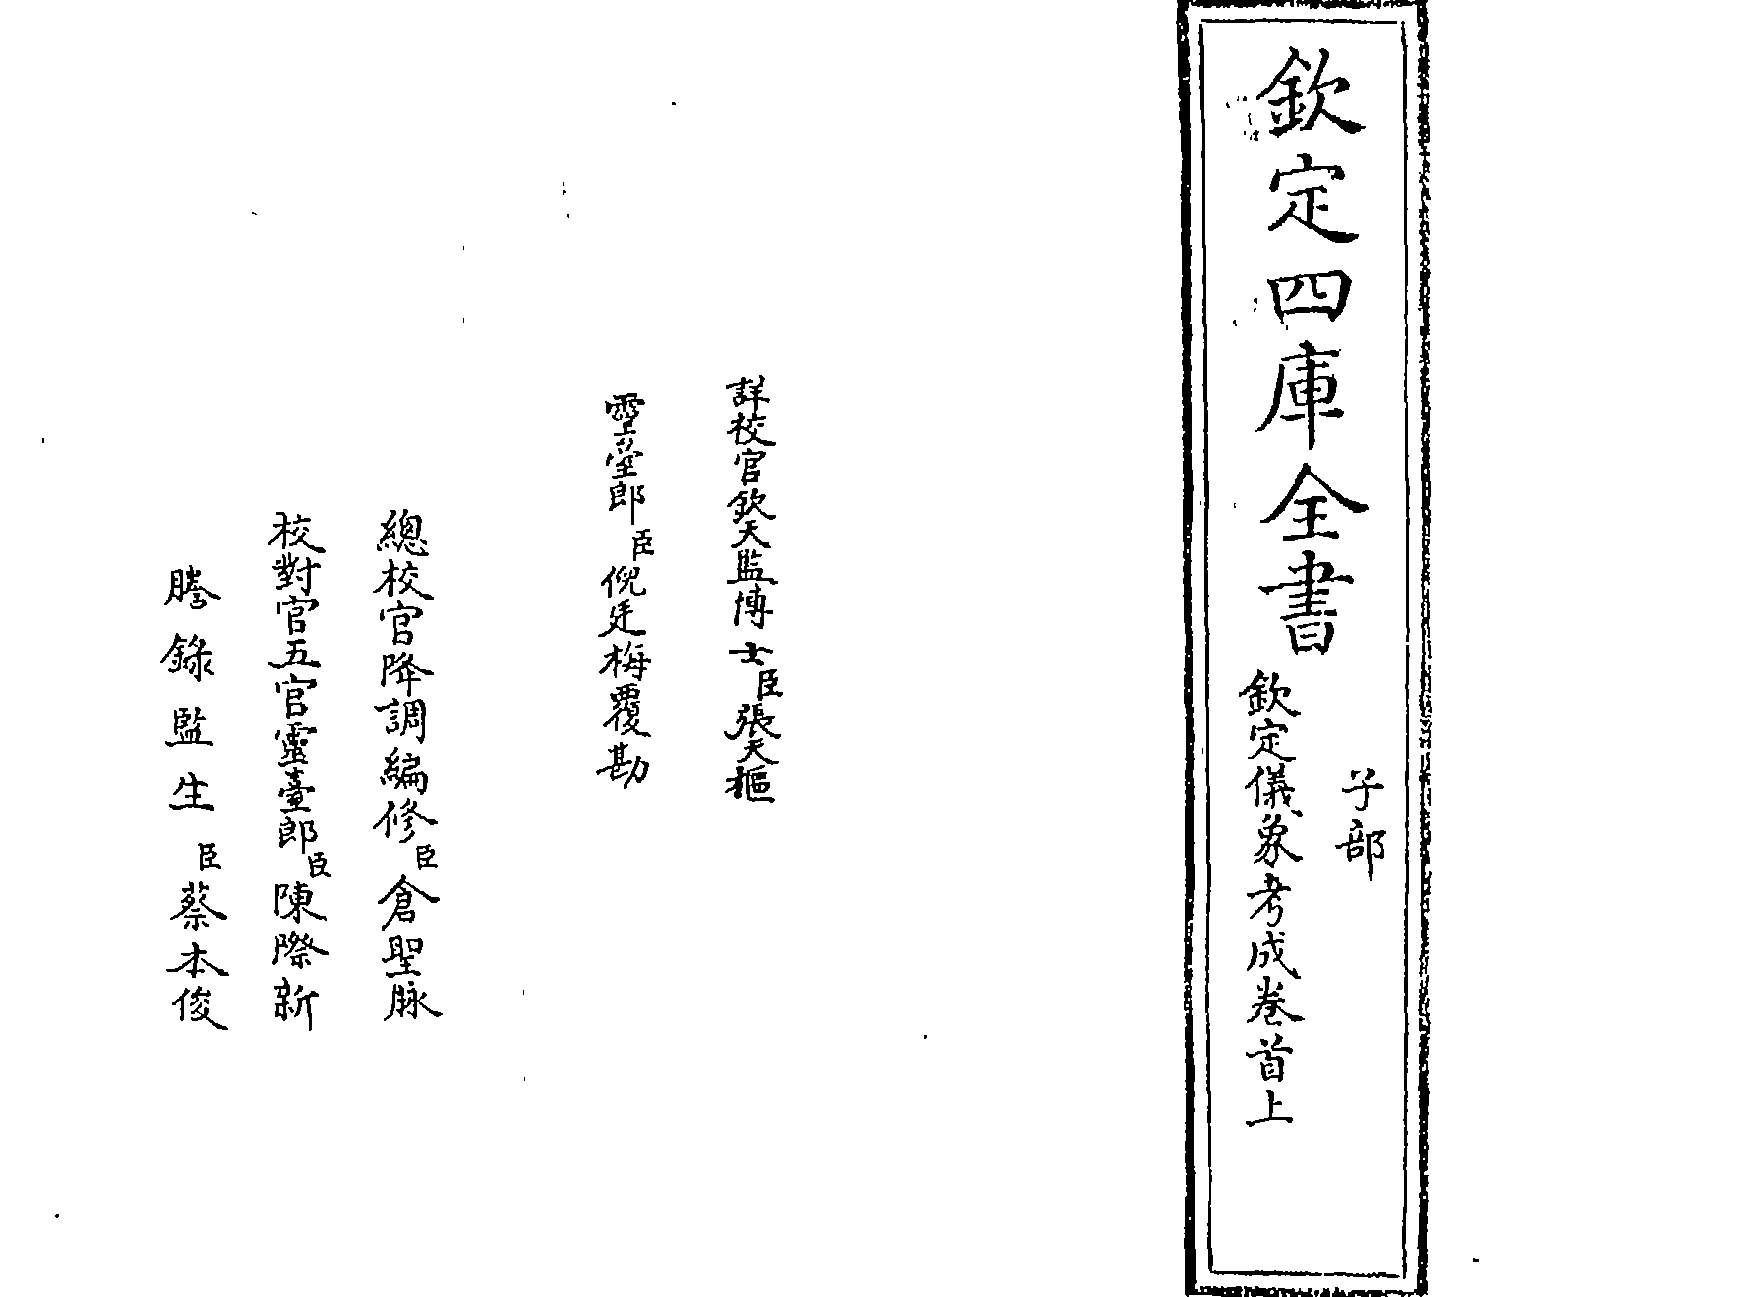
\includegraphics[width=\paperwidth,height=\paperheight,keepaspectratio]{img/0092.png}\clearpage
\begin{正文}
% ---- 册793 葉93 ----
\SetPageNumber{1}
欽定四庫全書\换行
欽定儀象考成卷首上\换行
御製璣衡撫辰儀説卷上\换行
　　儀制\换行
　　製法\换行
\char"200B\relax\换行
\char"200B\relax\换行
\char"200B\relax\换行
\char"200B\relax\换行
\char"200B\relax\换行
\char"200B\relax\换行
\char"200B\relax\换行
\char"200B\relax\换行
\char"200B\relax\换行
\char"200B\relax\换行
\char"200B\relax
\par
% ---- 册793 葉96 ----
御製璣衡撫辰儀説卷上之一\换行
　儀制\换行
　　全儀\换行
　　子午圏\换行
　　天常赤道\换行
　　赤極經圏\换行
　　遊旋赤道\换行
　　四遊圏\换行
　　指時度表\换行
　　借弧指時度表\换行
　　指緯度表\换行
　　立表\换行
　　平行立表\换行
　　平行借弧表\换行
　　綰經度表\换行
　　綰時度表
\par
% ---- 册793 葉97 ----
　　平行線測經度表\换行
\char"200B\relax\换行
\char"200B\relax\换行
\char"200B\relax\换行
\char"200B\relax\换行
\char"200B\relax\换行
\char"200B\relax\换行
\char"200B\relax\换行
\char"200B\relax\换行
\char"200B\relax\换行
\char"200B\relax\换行
\char"200B\relax\换行
\char"200B\relax\换行
\char"200B\relax\换行
\char"200B\relax\换行
\char"200B\relax
\par
\end{正文}\clearpage
\嵌图{153.00pt}{215.88pt}{395.02pt}{576.95pt}{img/0100.png}
\begin{正文}
% ---- 册793 葉100 ----
\SetPageNumber{4}
\插图页
\char"200B\relax\换行
\char"200B\relax\换行
\char"200B\relax\换行
\char"200B\relax\换行
\char"200B\relax\换行
\char"200B\relax\换行
\char"200B\relax\换行
\char"200B\relax\换行
\恢复丝栏
　　虞書舜典在璿璣玉衡以齊七政孔穎逹疏曰璣\换行
　　衡者王者正天文之器漢世以來謂之渾天儀者\换行
　　是也馬融云渾天儀可旋轉故曰璣衡其横簫所\换行
　　以視星宿也蔡邕云衡長八尺孔徑一寸下端望\换行
　　之以視星辰盖懸璣以象天而衡望之轉璣窺衡\换行
　　以知星宿是其説也上天之體不可得知測天之\换行
　　事見於經者惟此璿璣玉衡一事而已楊子法言\换行
　　云或問渾天曰落下閎營之鮮于妄人度之耿中
\par
% ---- 册793 葉101 ----
　　丞象之幾乎幾乎莫之能違也閎與妄人武帝時\换行
　　人宣帝時司農中丞耿夀昌始鑄銅為之象史官\换行
　　施用焉江南宋元嘉年太史丞錢樂\双列{\右小列{陳氏師凱曰}\左小列{錢樂本名樂}}\换行
　　\双列{\右小列{之孔疏}\左小列{脱之字}}鑄銅作渾天儀傳於齊梁周平江陵遷於\换行
　　長安尚書蔡註曰宋錢樂鑄銅作渾天儀衡長八\换行
　　尺孔徑一寸璣徑八尺圓周二丈五尺强轉而望\换行
　　之以知日月星辰之所在即璿璣玉衡之遺法也\换行
　　厯代以來其法漸密本朝因之為儀三重其在外\换行
　　者曰六合儀平置黒單環上刻十二辰八干四隅\换行
　　在地之位以凖地面而定四方側立黒雙環背刻\换行
　　去極度數以中分天脊直跨地平使其半入地下\换行
　　而結於其子午以為天經斜倚赤單環背刻赤道\换行
　　度數以平分天腹横繞天經亦使半出地上半入\换行
　　地下而結於其卯酉以為天緯三環表裏相結不\换行
　　動其天經之環則南北二極皆為圓軸虚中而内\换行
　　向以挈三辰四遊之環以其上下四方於是可考
\par
% ---- 册793 葉104 ----
　　故曰六合次其内曰三辰儀側立黒雙環亦刻去\换行
　　極度數外貫天經之軸内挈黄赤二道其赤道則\换行
　　為赤單環外依天緯亦刻宿度而結於黒雙環之\换行
　　卯酉其黄道則為黄單環亦刻宿度而又斜倚於\换行
　　赤道之腹以交結於卯酉而半入其内以為春分\换行
　　後之日軌半出其外以為秋分後之日軌又為白\换行
　　單環以承其交使不傾墊以其日月星辰於是可\换行
　　考故曰三辰其最在内者曰四遊儀亦為黒雙環\换行
　　如三辰儀之制以貫天經之軸其環之内則兩面\换行
　　當中各施直距外指兩軸而當其要中之内面又\换行
　　為小窽以受玉衡要中之小軸使衡既得隨環東\换行
　　西運轉又可隨處南北低昻以待占𠉀者之仰窺\换行
　　焉以其東西南北無不周徧故曰四遊此其法之\换行
　　大畧也今考前史漢初落下閎造渾天儀本無黄\换行
　　道或云賈逵所加或云李淳風所加或云一行所\换行
　　加而宋錢樂之渾儀之制雖有黄道並無黄道經
\par
% ---- 册793 葉105 ----
　　圈其四遊圈亦不貫於黄極則亦未盡黄道之用\换行
　　元郭守敬作簡儀乃分渾儀而變其制别設立運\换行
　　圏以測地平經緯度而不設黄道圏盖黄道與黄\换行
　　極經圏成經緯設黄道又設經圏則圏多而不便\换行
　　於測𠉀故不用黄道而專用赤道圈明正統三年\换行
　　　鑄銅渾儀簡儀於北京即宋元遺法也我\换行
　　朝康熙八年\换行
\抬头[1]聖祖仁皇帝命監臣南懐仁新製六儀赤道黄道分為二\换行
　　器皆不用地平圏而地平象限天體諸儀則地平\换行
　　之經緯與黄赤之錯綜皆已畢具康熙五十二年\换行
　　　又\换行
\抬头[1]命監臣紀利安製地平經緯儀合地平象限二儀而為一\换行
　　　其用尤便制作之妙於斯極矣我\换行
　皇上敬\换行
天法\换行
祖齊政勤民
\par
% ---- 册793 葉108 ----
親蒞靈臺徧觀儀象以渾天制最近古而時度信宜從\换行
　　今觀其㑹通斯成鉅典於是用今之數目合古之\换行
　　型模\换行
御製璣衡撫辰儀用裨測𠉀誠唐虞之遺意昭代之新\换行
　　規也儀制三重其在外者即古之六合儀而不用\换行
　　地平圏其正立雙環為子午圏兩面皆刻周天三\换行
　　百六十度自南北極起初度至中要九十度是為\换行
　　天經斜倚單環為天常赤道圏兩面皆刻周日十\换行
　　二時以子正午正當子午雙環中空之半而結於\换行
　　其中要是為天緯其南北二極皆設圓軸軸本實\换行
　　於子午雙環中空之間而軸内向以貫内二重之\换行
　　環其下承以雲座仰面正中開雙槽以受雙環東\换行
　　面正中開雲窩以受垂球下面置十字架施螺旋\换行
　　以取平架之東西兩端各植龍柱龍口銜珠開孔\换行
　　以承天常赤道卯酉之兩軸依觀象臺測定南北\换行
　　正線将座架安定則平面之四方正又依京師北
\par
% ---- 册793 葉109 ----
　　極出地三十九度五十五分自北極而上五十度\换行
　　五分即上應天頂自南極而下五十度五分即下\换行
　　對地心而應天頂之衝於天頂施小釘懸垂線而\换行
　　垂適當地心又適切於雙環之面不即不離則上\换行
　　下正立面之四方亦正而地平已在其中故不用\换行
　　地平圏也次其内即古之三辰儀而不用黄道圏\换行
　　其貫於二極之雙環為赤極經圏兩極各設軸孔\换行
　　以受天經之軸兩面皆刻周天三百六十度結於\换行
　　赤極經圏之中要與天常赤道平運者為遊旋赤\换行
　　道圈兩面皆刻周天三百六十度與天之赤道旋\换行
　　轉相應自經圏之南極作兩象限弧以承之使不\换行
　　傾墊測得三辰之赤道經緯度則黄道經緯可推\换行
　　且黄道與赤道之相距古逺今近縱或日久有差\换行
　　而儀器無庸改制故不用黄道圏也其在内者即\换行
　　古之四遊儀貫於二極之雙環為四遊圏兩面皆\换行
　　刻三百六十度定於遊圏之兩極者為直距綰於
\par
% ---- 册793 葉112 ----
　　直距之中心者為窺衡遊圏中要設直表以指經\换行
　　度及時窺衡右旁設直表以指緯度此古今所同\换行
　　無容置議者也是故體制倣乎渾天之舊而時度\换行
　　尤為整齊運量同於赤道新儀而重環更能合應\换行
　　至於借表窺測則上下左右無不宜焉夫羲和遺\换行
　　制不可考已漢世以來或作而不傳或傳而不久\换行
　　盖制器尚象若斯之難也而稽古宜今至我\换行
　朝乃臻盡善易繫傳云備物致用立成器以為天下\换行
　　利莫大乎聖人詎不信乎\换行
\char"200B\relax\换行
\char"200B\relax\换行
\char"200B\relax\换行
\char"200B\relax\换行
\char"200B\relax\换行
\char"200B\relax\换行
\char"200B\relax
\par
\end{正文}\clearpage
\嵌图{154.79pt}{220.57pt}{393.23pt}{572.26pt}{img/0118.png}
\begin{正文}
% ---- 册793 葉118 ----
\SetPageNumber{11}
\插图页
\char"200B\relax\换行
\char"200B\relax\换行
\char"200B\relax\换行
\char"200B\relax\换行
\char"200B\relax\换行
\char"200B\relax\换行
\char"200B\relax\换行
\char"200B\relax\换行
\恢复丝栏
子午圈所以正南北也天之南北定於兩極必先測定\换行
南北正線而後安置子午圈則子午圈即為南北之正\换行
線南北正而後日軌之髙下時刻之早晚中星之偏度\换行
可得而稽也其制雙環外徑六尺三寸内徑五尺六寸\换行
六分環面濶三寸二分厚九分中空一寸雙環之間四\换行
隅各施銅枕合而固之其中空之半為子午正線兩面\换行
各畫三百六十度每度六十分自南北極起初度至中\换行
要九十度古曰天經環西法舊曰緯圈盖織絲以直者
\par
% ---- 册793 葉122 ----
為經横者為緯古以其圈直立故曰經西法以其為横\换行
線所界之度故曰緯今按圈直而度横則其圈宜曰經\换行
圈而其度乃為緯度周禮賈公彦疏所謂南北之道謂\换行
之經元儒陳氏師凱所謂自北數向南去如機上數緯\换行
絲是也自兩極起初度者北極出地南極入地其度數\换行
皆自兩極起算也中要九十度者赤道為帯天之紘距\换行
兩極各一象限也南北極各設鋼軸軸本扁方長三寸\换行
濶二寸二分厚一寸實於隻環之間以鋼螺旋結之軸\换行
長六寸徑八分正當雙環中空之半内向以貫三辰四\换行
遊之環所以象天樞也\换行
\char"200B\relax\换行
\char"200B\relax\换行
\char"200B\relax\换行
\char"200B\relax\换行
\char"200B\relax\换行
\char"200B\relax
\par
\end{正文}\clearpage
\嵌图{148.32pt}{219.14pt}{399.70pt}{573.69pt}{img/0126.png}
\begin{正文}
% ---- 册793 葉126 ----
\SetPageNumber{13}
\插图页
\char"200B\relax\换行
\char"200B\relax\换行
\char"200B\relax\换行
\char"200B\relax\换行
\char"200B\relax\换行
\char"200B\relax\换行
\char"200B\relax\换行
\char"200B\relax\换行
\恢复丝栏
天常赤道所以正時刻也天左旋一日一周南北極持\换行
其兩端而赤道為其横帯以其常定不動故曰天常日\换行
循黄道右旋而其隨天西轉則係赤道之度日行臨於\换行
赤道之某位即為某時故時刻由赤道而正也其制單\换行
環外徑六尺一寸二分内徑五尺六寸四分環面濶二\换行
寸四分厚一寸四分平分其厚為赤道之中線兩面各\换行
畫周日十二時每時初正各四刻每刻十五分每一時\换行
當天之三十度每四刻當天之十五度每一分當天之
\par
% ---- 册793 葉130 ----
十五分以其子正午正線當子午雙環中空之半而結\换行
於其中要使其赤道中線適當子午圏之九十度兩圈\换行
相結成十字直角古曰天緯環西法舊曰赤道經圈盖\换行
古以其圈横運故曰緯西法以其為直線所界之度故\换行
曰經今按圈横而度直則其圈宜曰緯圈而其度乃為\换行
經度周禮賈公彦疏所謂東西之道謂之緯陳氏師凱\换行
所謂自東數向西去如機上數經絲是也上面午正時\换行
刻線結於子午圈之正北卯正居西酉正居東謂日影\换行
對照之時下面則子正居北午正居南卯正居東酉正\换行
居西為日行所臨之正位也\换行
\char"200B\relax\换行
\char"200B\relax\换行
\char"200B\relax\换行
\char"200B\relax\换行
\char"200B\relax\换行
\char"200B\relax
\par
\end{正文}\clearpage
\嵌图{153.38pt}{219.23pt}{394.64pt}{573.60pt}{img/0134.png}
\begin{正文}
% ---- 册793 葉134 ----
\SetPageNumber{15}
\插图页
\char"200B\relax\换行
\char"200B\relax\换行
\char"200B\relax\换行
\char"200B\relax\换行
\char"200B\relax\换行
\char"200B\relax\换行
\char"200B\relax\换行
\char"200B\relax\换行
\恢复丝栏
赤極經圏所以帯赤道也亦曰過極圏制如子午雙環\换行
在内而差小外徑五尺五寸六分内徑五尺一寸二分\换行
環面濶二寸二分厚八分中空一寸二分兩面皆畫三\换行
百六十度每度六十分一面自兩極起初度至赤道九\换行
十度以應天經一面自赤道起初度至兩極九十度以\换行
應赤緯南北極各設軸孔用扁方銅長三寸濶與環面\换行
等厚與雙環中空等中心開圓孔以受天經之軸其孔\换行
徑適容軸徑使旋轉不致動摇孔之兩面各施鋼片厚
\par
% ---- 册793 葉138 ----
四分使孔徑不致磨損兩軸孔之中徑適當雙環中空\换行
之半與兩極徑線參直以鋼螺旋結之環外南北極之\换行
兩端各施扁圓鋼子厚五分與内外兩雙環之分縫等\换行
貫於天經之軸使赤極經圈之中要九十度線適與子\换行
午圈之九十度相凖則内外兩圈上下四方俱合為一\换行
線而縱横經緯自宜悉協矣\换行
\char"200B\relax\换行
\char"200B\relax\换行
\char"200B\relax\换行
\char"200B\relax\换行
\char"200B\relax\换行
\char"200B\relax\换行
\char"200B\relax\换行
\char"200B\relax\换行
\char"200B\relax\换行
\char"200B\relax
\par
\end{正文}\clearpage
\嵌图{157.41pt}{218.38pt}{390.61pt}{574.45pt}{img/0142.png}
\begin{正文}
% ---- 册793 葉142 ----
\SetPageNumber{17}
\插图页
\char"200B\relax\换行
\char"200B\relax\换行
\char"200B\relax\换行
\char"200B\relax\换行
\char"200B\relax\换行
\char"200B\relax\换行
\char"200B\relax\换行
\char"200B\relax\换行
\恢复丝栏
遊旋赤道所以象天之運行而紀其赤道經度也制如\换行
天常赤道在内而差小外徑五尺五寸六分内徑五尺\换行
一寸二分環面濶二寸二分厚一寸二分平分其厚為\换行
赤道之中線兩面各畫周天三百六十度上面分為十\换行
二宫每宫三十度每度六十分下面自丑宫起初度右\换行
旋三百六十度以其丑宫未宫初度之線當赤經雙環\换行
中空之半而結於其中要使其赤道中線適當經圈之\换行
九十度兩圈相結成十字直角與天之赤道旋轉相應
\par
% ---- 册793 葉146 ----
又於經圏南極之兩旁設象限弧承於遊旋赤道辰宫\换行
戌宫之下以螺旋結之使不傾墊有天常赤道之不動\换行
者以定時又有遊旋赤道之常動者以紀度則赤道之\换行
逐宫逐度皆能周行於十二時而三辰之所躔與兩曜\换行
之相距皆可得而稽矣\换行
\char"200B\relax\换行
\char"200B\relax\换行
\char"200B\relax\换行
\char"200B\relax\换行
\char"200B\relax\换行
\char"200B\relax\换行
\char"200B\relax\换行
\char"200B\relax\换行
\char"200B\relax\换行
\char"200B\relax\换行
\char"200B\relax
\par
\end{正文}\clearpage
\嵌图{152.17pt}{219.82pt}{395.85pt}{573.01pt}{img/0150.png}
\begin{正文}
% ---- 册793 葉150 ----
\SetPageNumber{19}
\插图页
\char"200B\relax\换行
\char"200B\relax\换行
\char"200B\relax\换行
\char"200B\relax\换行
\char"200B\relax\换行
\char"200B\relax\换行
\char"200B\relax\换行
\char"200B\relax\换行
\恢复丝栏
四遊圈所以測三辰之赤道經緯度也制如赤經雙環\换行
在内而差小外徑五尺内徑四尺六寸八分環面濶一\换行
寸六分厚七分中空一寸四分盖三重雙環之外面皆\换行
相平而内重則漸薄中空則漸大取其輕重適宜亦便\换行
於設窺衡也兩面各畫三百六十度一面自北極起初\换行
度至南極一百八十度為去極度一面自赤道起初度\换行
至兩極各九十度為距緯度南北極各設軸孔以受夭\换行
經之軸與過極圈同環外南北極之兩端各施扁圓鋼
\par
% ---- 册793 葉152 ----
子厚六分與赤經四遊兩環之分縫等貫於天經之軸\换行
其下半周之中要安直表以指經度及時刻兩面對南\换行
北極各安直距如圓之通徑濶一寸六分厚七分中空\换行
一寸四分直距之二面對環之兩極作直徑線對環之\换行
九十度作横徑線十字相交中心開圓孔施螺旋小鋼\换行
軸而圓其末以綰窺衡窺衡長四尺七寸二分方一寸\换行
二分中空一寸上下兩端施方銅盖厚五分内三分方\换行
一寸入於管中外二分方一寸二分齊於管面中心開\换行
圓孔上端孔心留十字線以便測視管之四面亦各取\换行
中線上面安立表下端右面安指緯度表左右兩面之\换行
中心各開圓孔使直距中要小軸之末入其中以綰之\换行
則窺衡乃能南北低昂而隨雙環東西運轉焉窺衡連\换行
盖長四尺七寸六分比四遊環内徑長八分兩端各施\换行
鋼篐厚一分中要孔外施鋼眼錢亦厚一分使其左右\换行
適切於中空之内面上下兩端入於雙環内徑各四分\换行
則上下低昂自無偏側而所測經緯度必皆密合矣
\par
\end{正文}\clearpage
\嵌图{153.29pt}{217.38pt}{394.73pt}{575.45pt}{img/0153.png}
\begin{正文}
% ---- 册793 葉153 ----
\SetPageNumber{21}
\插图页
\char"200B\relax\换行
\char"200B\relax\换行
\char"200B\relax\换行
\char"200B\relax\换行
\char"200B\relax\换行
\char"200B\relax\换行
\char"200B\relax\换行
\char"200B\relax\换行
\恢复丝栏
指時度表通長七寸三分本長一寸六分形如方筒入\换行
於四遊雙環中空之間濶一寸四分與四遊環之中空\换行
等平分其濶即當窺衡之中線筒中施左右螺旋以充\换行
塞於中空之内使表不動移横帶長三寸二分濶五分\换行
兩端各鉤囬二分扣於環面之外表長五寸二分濶一\换行
寸其指時度之邊線對方筒之正中亦即窺衡之正中\换行
下端二寸四分厚三分切於遊旋赤道之面以指度分\换行
上端二寸八分厚二分切於天常赤道之面以指時刻
\par
% ---- 册793 葉156 ----
也\换行
\char"200B\relax\换行
\char"200B\relax\换行
\char"200B\relax\换行
\char"200B\relax\换行
\char"200B\relax\换行
\char"200B\relax\换行
\char"200B\relax\换行
\char"200B\relax\换行
\char"200B\relax\换行
\char"200B\relax\换行
\char"200B\relax\换行
\char"200B\relax\换行
\char"200B\relax\换行
\char"200B\relax\换行
\char"200B\relax
\par
\end{正文}\clearpage
\嵌图{151.20pt}{217.28pt}{396.82pt}{575.55pt}{img/0157.png}
\begin{正文}
% ---- 册793 葉157 ----
\SetPageNumber{23}
\插图页
\char"200B\relax\换行
\char"200B\relax\换行
\char"200B\relax\换行
\char"200B\relax\换行
\char"200B\relax\换行
\char"200B\relax\换行
\char"200B\relax\换行
\char"200B\relax\换行
\恢复丝栏
借弧指時度表其本方筒及横帶長濶並與前指時度\换行
表同横帶之下自左向右立安弧背一道長九寸三分\换行
濶一寸二分厚一分六釐弧背之末平安指時度表除\换行
弧背之厚長五寸二分濶一寸計自表本方筒之中線\换行
至指時度表之内邊長六寸七分當遊旋赤道之十五\换行
度當天常赤道之一小時測量時指時度表或為子午\换行
圏所礙則用此表視其所指之時度加四刻即為所測\换行
之時減十五度即為所測之度盖借弧指時度表在窺
\par
% ---- 册793 葉160 ----
衡之右所指雖視乎借表而所測則定於窺衡天常之\换行
時刻左旋故加三辰之度分右旋故減則用借弧指時\换行
度表察之與用指時度表等也\换行
\char"200B\relax\换行
\char"200B\relax\换行
\char"200B\relax\换行
\char"200B\relax\换行
\char"200B\relax\换行
\char"200B\relax\换行
\char"200B\relax\换行
\char"200B\relax\换行
\char"200B\relax\换行
\char"200B\relax\换行
\char"200B\relax\换行
\char"200B\relax\换行
\char"200B\relax
\par
\end{正文}\clearpage
\嵌图{151.20pt}{220.43pt}{396.82pt}{572.40pt}{img/0161.png}
\begin{正文}
% ---- 册793 葉161 ----
\SetPageNumber{25}
\插图页
\char"200B\relax\换行
\char"200B\relax\换行
\char"200B\relax\换行
\char"200B\relax\换行
\char"200B\relax\换行
\char"200B\relax\换行
\char"200B\relax\换行
\char"200B\relax\换行
\恢复丝栏
指緯度表其形兩曲安於窺衡下端之右面底長三寸\换行
濶九分平分其濶為中線對衡面中線以螺旋結之曲\换行
横七分與四遊環之厚等又曲長一寸七分切於四遊\换行
環之外面從中線減濶之半所以指緯度也\换行
\char"200B\relax\换行
\char"200B\relax\换行
\char"200B\relax\换行
\char"200B\relax
\par
\end{正文}\clearpage
\嵌图{153.29pt}{219.54pt}{394.73pt}{573.29pt}{img/0164.png}
\begin{正文}
% ---- 册793 葉164 ----
\SetPageNumber{26}
\插图页
\char"200B\relax\换行
\char"200B\relax\换行
\char"200B\relax\换行
\char"200B\relax\换行
\char"200B\relax\换行
\char"200B\relax\换行
\char"200B\relax\换行
\char"200B\relax\换行
\恢复丝栏
立表二座形直底平表髙底長各三寸二分濶九分厚\换行
一分平分其濶為中線表直立於底長之半與底面成\换行
直角距底面一寸一表向上開長方孔長一寸中留直\换行
線又上五分開圓孔徑四分中留十字線安於窺衡之\换行
上端一表依前度下開直縫上開小圓孔安於窺衡之\换行
下端各對衡面中線以螺旋結之測量時窺衡或為赤\换行
道及銅枕所礙則用此表盖兩表之孔心中線距衡面\换行
皆相等又與衡面之中線參直則用立表測之與用窺
\par
% ---- 册793 葉165 ----
衡等也\换行
\char"200B\relax\换行
\char"200B\relax\换行
\char"200B\relax\换行
\char"200B\relax\换行
\char"200B\relax\换行
\char"200B\relax\换行
\char"200B\relax\换行
\char"200B\relax\换行
\char"200B\relax\换行
\char"200B\relax\换行
\char"200B\relax\换行
\char"200B\relax\换行
\char"200B\relax\换行
\char"200B\relax\换行
\char"200B\relax
\par
\end{正文}\clearpage
\嵌图{153.00pt}{217.70pt}{395.02pt}{575.13pt}{img/0168.png}
\begin{正文}
% ---- 册793 葉168 ----
\SetPageNumber{28}
\插图页
\char"200B\relax\换行
\char"200B\relax\换行
\char"200B\relax\换行
\char"200B\relax\换行
\char"200B\relax\换行
\char"200B\relax\换行
\char"200B\relax\换行
\char"200B\relax\换行
\恢复丝栏
平行立表二座形曲底平底盤長四寸濶一寸二分厚\换行
一分中空長三寸二分濶九分與立表底盤之長濶等\换行
表曲如勾股股直如立表髙三寸二分濶九分勾横連\换行
於股末長五寸濶九分横植於底盤之末底盤中空冒\换行
於立表底盤之外以掐表固之測量時窺衡立表或為\换行
子午圏及龍柱所礙則用此表盖平行立表曲如勾股\换行
而與立表平行則用平行立表測之與用立表等亦與\换行
用窺衡等也
\par
\end{正文}\clearpage
\嵌图{153.00pt}{223.19pt}{395.02pt}{569.64pt}{img/0169.png}
\begin{正文}
% ---- 册793 葉169 ----
\SetPageNumber{29}
\插图页
\char"200B\relax\换行
\char"200B\relax\换行
\char"200B\relax\换行
\char"200B\relax\换行
\char"200B\relax\换行
\char"200B\relax\换行
\char"200B\relax\换行
\char"200B\relax\换行
\恢复丝栏
平行借弧表制如平行立表而倒正異盖四遊窺衡東\换行
西為子午圏及龍柱所礙南北為赤道及銅枕所礙則\换行
用平行立表猶是窺衡所能及而管孔被遮故其表平\换行
行正立即可見若近北極之星則東西既礙於子午圏\换行
南北又礙於極軸窺衡不能及自上測之不能及北極\换行
之南六度餘自下測之不能及北極之北六度餘故借\换行
十度作平行借弧表一表上植一表下垂則窺衡未及\换行
北極十度而窺孔之視線已與北極參直其法以半徑
\par
% ---- 册793 葉172 ----
一千萬為一率十度之正切線一百七十六萬三千二\换行
百七十為二率表之横勾距窺衡中心二尺三寸三分\换行
為三率求得四率四寸一分零八毫為表髙之中數\双列{\右小列{自}\左小列{窺}}\换行
\双列{\右小列{衡中線至直}\左小列{距中線之數}}上端之表立植於衡面則中數即表髙\双列{\右小列{中}\左小列{數}}\换行
\双列{\右小列{減衡方之半六分加表端距窺孔中心}\左小列{六分為表端至表本之髙仍與中數等}}下端之表自衡\换行
面下垂則於中數加衡方之半六分表端距窺孔中心\换行
六分又加平行横勾之濶九分得六寸二分零八毫為\换行
表之髙距表端下六分開圓孔又下五分開長方孔皆\换行
與立表制同凡測近北極之星測得距赤道北若干加\换行
十度即得星距赤道北之緯度若測赤道南之星亦可\换行
用此表但測得距赤道南若干減十度即得星距赤道\换行
南之緯度也\换行
\char"200B\relax\换行
\char"200B\relax\换行
\char"200B\relax\换行
\char"200B\relax
\par
\end{正文}\clearpage
\嵌图{155.09pt}{220.28pt}{392.93pt}{572.55pt}{img/0173.png}
\begin{正文}
% ---- 册793 葉173 ----
\SetPageNumber{31}
\插图页
\char"200B\relax\换行
\char"200B\relax\换行
\char"200B\relax\换行
\char"200B\relax\换行
\char"200B\relax\换行
\char"200B\relax\换行
\char"200B\relax\换行
\char"200B\relax\换行
\恢复丝栏
綰經度表通長四寸濶一寸四分平分其濶即當窺衡\换行
之中線其本方筒長一寸六分髙一寸八分入於四遊\换行
雙環之間以左右螺旋固之其末上下二面以夾遊旋\换行
赤道上面濶七分減本之半與窺衡中線參直下面以\换行
螺旋固之所以綰定遊旋赤道之經度於四遊圈也\换行
\char"200B\relax\换行
\char"200B\relax\换行
\char"200B\relax
\par
\end{正文}\clearpage
\嵌图{153.29pt}{222.42pt}{394.73pt}{570.41pt}{img/0176.png}
\begin{正文}
% ---- 册793 葉176 ----
\SetPageNumber{32}
\插图页
\char"200B\relax\换行
\char"200B\relax\换行
\char"200B\relax\换行
\char"200B\relax\换行
\char"200B\relax\换行
\char"200B\relax\换行
\char"200B\relax\换行
\char"200B\relax\换行
\恢复丝栏
綰時度表内外二截内截上下内三面綰於遊旋赤道\换行
之内規上面之末承於外截之下開二方孔以受外截\换行
之方足下面以螺旋固之外截上下外三面綰於天常\换行
赤道之外規上面之末覆於内截之上安二方足入於\换行
内截之方孔下面以螺旋固之凡以太陽時刻及經度\换行
測月星則内外截俱綰定别測月星若以經度求時刻\换行
則止綰定内截外截隨之運轉視其所當刻分即得時\换行
刻若以時刻求經度則止綰定外截任遊旋赤道之運
\par
% ---- 册793 葉177 ----
轉視其所當度分即得經度也\换行
\char"200B\relax\换行
\char"200B\relax\换行
\char"200B\relax\换行
\char"200B\relax\换行
\char"200B\relax\换行
\char"200B\relax\换行
\char"200B\relax\换行
\char"200B\relax\换行
\char"200B\relax\换行
\char"200B\relax\换行
\char"200B\relax\换行
\char"200B\relax\换行
\char"200B\relax\换行
\char"200B\relax\换行
\char"200B\relax
\par
\end{正文}\clearpage
\嵌图{146.46pt}{204.81pt}{838.85pt}{580.16pt}{img/0180.png}
\begin{正文}
% ---- 册793 葉180 图版 ----
\SetPageNumber{34}
\插图页
\char"200B\relax\换行
\char"200B\relax\换行
\char"200B\relax\换行
\char"200B\relax\换行
\char"200B\relax\换行
\char"200B\relax\换行
\char"200B\relax\换行
\char"200B\relax\换行
\char"200B\relax\换行
\char"200B\relax\换行
\char"200B\relax\换行
\char"200B\relax\换行
\char"200B\relax\换行
\char"200B\relax\换行
\char"200B\relax\换行
\char"200B\relax
\恢复丝栏\par
% ---- 册793 葉181 ----
平行線測經度表以赤經之平行線與直距之平行線\换行
相參直\双列{\右小列{赤經之平行線在圓周直距之平行線在}\左小列{圓心其平行線之間俱對南北極之中徑}}而測\换行
距星之經度也其制於直距南北極之兩端各安銅板\换行
如工字形正方二寸八分與直距二面之分等\双列{\右小列{直距二}\左小列{面各厚}}\换行
\双列{\右小列{七分中空一寸四}\左小列{分共二寸八分}}兩要各缺一長方長一寸六分濶七\换行
分與直距一面之分等\双列{\右小列{直距二面每面濶}\左小列{一寸六分厚七分}}扣於直距中\换行
空之間中心開圓孔貫於天經之軸四隅距中心一寸\换行
九分\双列{\右小列{銅板方二寸八分對角斜線三寸九分八釐四隅}\左小列{距中心各一寸九分九釐今取一寸九分餘九釐}}\换行
各安立柱圓頂開孔以穿直線與直距中徑平行下安\换行
小環以為結赤經平行線之用又按距星宫度於遊旋\换行
赤道安赤經平行線表其制上畫半圓内容半方自對\换行
角斜線起初度至横徑為四十五度其中直徑與指度\换行
表之邊線參直半圓中心安二遊表各長二寸距中心\换行
一寸九分邊留小臍中開小圓孔與直距四隅立柱之\换行
距中心等以線穿之上端繫於北極銅板對角之兩環\换行
下端貫於南極銅板對角之兩環各以垂球墜之乃視
\par
% ---- 册793 葉184 ----
四遊圏之所測與此平行線之所測相距若干度即将\换行
遊表對半圓度數安定下面以螺旋中徑以壓表固之\换行
此二線必與赤經中徑平行而與直距中徑之二平行\换行
線廣狹相等從左線視之與所測參直從右線視之亦\换行
與所測參直則此二線即為距星經度之凖線以此線\换行
對定距星将遊旋赤道隨之運轉又以四遊圏及窺管\换行
測日月及星即得其經緯度也盖以一星作距測日月\换行
及星必用兩測舊制黄道赤道二儀南北極之通徑皆\换行
係圓軸故測𠉀用通光耳實其正中與軸徑等兩邊各\换行
開直縫從左縫對軸左邊見光從右縫對軸右邊見光\换行
亦猶用平行線之意也今不用圓軸而用直距兩測相\换行
距有逺近則直距對角有斜横斜則二線平距之分狹\换行
横則二線平距之分廣\双列{\右小列{直鉅銅板方分也其對角斜分}\左小列{也二線平距則横分也對角斜}}\换行
\双列{\右小列{則平距為斜之方故狹對角}\左小列{横則平距為方之斜故廣}}其限自正斜起初度至四\换行
十五度而横四十五度以後復由横而斜至九十度與\换行
初度同\双列{\右小列{九十度以後復由斜而横至一百三十五度與}\左小列{四十五度同一百三十五度以後復由横而斜}}
\par
% ---- 册793 葉185 ----
\双列{\右小列{至一百八十度與初}\左小列{度同盈半周天而止}}如四遊環與平行線表同度是為\换行
初度是時直距對角正斜而其二線平距之分為斜之\换行
方此二線平距之最狹者也過此而四遊環距平行線\换行
表漸逺則直距對角漸横而二線平距漸廣至四遊環\换行
距平行線表四十五度則直距對角正横而其二線平\换行
距之分為方之斜此二線平距之最廣者也過此則直\换行
距對角又漸斜而二線平距又漸狹至九十度正斜而\换行
最狹故又與初度同也今欲使赤經平行線與直距平\换行
行線廣狹相等必以直距對角斜横之度合於赤道之\换行
半圓遊表二線距圓心各一寸九分通共三寸八分即\换行
直距銅板對角之斜分也半圓自内方之對角斜線起\换行
初度即直距對角之初度為正斜也半圓至横徑為四\换行
十五度即直距對角之四十五度為正横也設以二遊\换行
表通為一直表則與直距對角之斜横儼為一體但遊\换行
表在赤道若通為一直表則其線為赤道所礙而廣狹\换行
不靈且通為一表此端在横徑内彼端必在横徑外凡
\par
% ---- 册793 葉188 ----
斜線與十字線過心相交其彼端距横徑外之度與此\换行
端距横徑内之度必相等而距中徑之濶亦相等故以\换行
直表彼端當横徑外之度另用一遊表於横徑内按度\换行
安之其距中徑之濶必相等而與直距二平行線廣狹\换行
亦相等則用平行線表亦猶用通光耳之意也\换行
\char"200B\relax\换行
\char"200B\relax\换行
\char"200B\relax\换行
\char"200B\relax\换行
\char"200B\relax\换行
\char"200B\relax\换行
\char"200B\relax\换行
\char"200B\relax\换行
\char"200B\relax\换行
\char"200B\relax\换行
\char"200B\relax
\par
% ---- 册793 葉189 ----
御製璣衡撫辰儀説卷上之二\换行
　製法\换行
　　銅質宜精\换行
　　型制宜工\换行
　　鏇磨宜平\换行
　　取心宜中\换行
　　輕重宜審\换行
　　界度宜均\换行
　　兩徑合度\换行
　　合結均齊\换行
　　三重同心\换行
　　安置方正\换行
\char"200B\relax\换行
\char"200B\relax\换行
\char"200B\relax\换行
\char"200B\relax
\par
% ---- 册793 葉192 ----
　　銅質宜精\换行
凡鑄黄銅器具應用紅銅六成倭鉛四成鎔錬精到然\换行
後鑄之遼厯象志云古之鍊銅黒黄白青之氣盡然後\换行
用之故可施於久逺唐一行鑄渾天儀時稱精妙理固\换行
然也\换行
　　型制宜工\换行
凡鑄儀器以土為型必先治地極平外規較定制微大\换行
内規較定制微小其外環面如輪次内如輻次内如轂\换行
中留環心務極圓平合度則所鑄之體自亦圓平而鏇\换行
磨亦易為力矣\换行
　　鏇磨宜平\换行
凡製儀器必用鏇磨圓環中心當治方孔以受軸軸圓\换行
而方其端施於環心之方孔使環之上下前後左右不\换行
得動揺則鏇之自圓且平矣\换行
　　取心宜中\换行
凡製圓器必取中心心中則界正未鏇之前環心尚在
\par
% ---- 册793 葉193 ----
圓規方孔皆自環心取中逮鏇之既成則無中心矣而\换行
畫儀器之圓線則必先取中心為凖須以直木為環徑\换行
其兩端即如環之内規切𦂳安定約其中心嵌定鐵板\换行
任於環之内規取三處作點用三點求圓心法\双列{\右小列{法見數}\左小列{理精藴}}\换行
求得圓心即於鐵板作記次以鋼製規徑一規尖二規\换行
尖之本開方孔貫於規徑之兩端一尖安於圓心一尖\换行
按環面内外規之度各用螺旋固之於環之内外規旋\换行
轉比試處處皆當規面則圓心中矣次依環之内外規\换行
取外界圓線半徑之度安定規尖畫外界圓線為度之\换行
外界即以此半徑度将外界圓線分為六觚毎觚六十\换行
度\双列{\右小列{半徑與六十}\左小列{度之通弦等}}又取内界圓線半徑之度安定規尖畫\换行
内界圓線為度之内界自外界每觚六十度之點平分\换行
之得三十度各對中心作直線抵内界其過心對角之\换行
線即圓之通徑而平分環面為兩半周則圓界正矣次\换行
将直線輕微引出外界至外規用極方正矩度凖於側\换行
面單環則自側面即凖於彼面雙環則自此環之側面
\par
% ---- 册793 葉196 ----
凖於彼環之側面復自彼環之側面凖於彼環之彼面\换行
輕微畫線作記乃用前直木環徑切𦂳安定以縱横二\换行
線對於所凖之通徑果於中心相交則所凖確合否則\换行
又用前法取心務令得中單環即可如前畫彼面之圓\换行
線及十二度線雙環則俟審定輕重合釘枕銅再行比\换行
試確凖然後可畫彼面也\换行
　　輕重宜審\换行
凡環之兩半周輕重適均則平置無偏側之失運轉無\换行
游移之弊審量之法用圓直鐵鋌徑八分\双列{\右小列{與軸}\左小列{徑等}}長逾環\换行
徑平分中線卧置之使不動移而以環面之通徑線加\换行
於其上易置試之兩半周無有低昂則輕重適均否則\换行
非其線有微差即其體質不等細察磨治務得其輕重\换行
之適均則天常赤道之子正午正遊旋赤道之丑宫未\换行
宫三雙環之南北極皆以此通徑為凖乃将雙環已畫\换行
十二度線之一面置於下以通徑凖線四象分中安設\换行
銅枕以雙環彼面之通徑凖線合於上釘而固之復用
\par
% ---- 册793 葉197 ----
前法比試確凖取定中心然後畫内外界圓線及十二\换行
度線則兩面之圓心圓界允協矣\换行
　　界度宜均\换行
環心既中環界既正則界度可得而均矣顧諸環皆取\换行
度分惟天常赤道取時刻然時刻亦與度分相凖故取\换行
度分者将每觚六十度平分之得三十度又三分之各\换行
為十度自外界抵内界各畫直線而於内界之外畫圓\换行
線一層是為十度界次将每十度又十分之各為一度\换行
自外界抵十度界各畫直線而於十度界之外外界之\换行
内各畫圓線一層是為度界次於内度界之外外度界\换行
之内各畫圓線一層為十分界将每度六分之各為十\换行
分畫直線於其界内次於内外兩十分界之間畫圓線\换行
九道界為十層自每十分之初至每十分之末各作對\换行
角斜線則每一圓線與斜線之交即逐度之一分也取\换行
時刻者每三十度為一時平分之得十五度為一小時\换行
每一小時分為四刻自外界抵内界各畫直線而於内
\par
% ---- 册793 葉200 ----
界之外畫圓線一層是為時刻界次将每刻十五分三\换行
分之各為五分自外界抵時刻界各畫直線而於時刻\换行
界之外外界之内各畫圓線一層是為五分界次於内\换行
五分界之外外五分界之内又各畫圓線一層為一分\换行
界而将每五分又各五分之各為一分畫直線與其界\换行
内次於内外兩一分界之間畫圓線十一道界為十二\换行
層自每一分之初至每一分之末作對角斜線則每一\换行
圓線與斜線之交即逐分之五秒也\双列{\右小列{每分為六十秒十}\左小列{二分之故為五秒}}\换行
　　兩徑合度\换行
界度既均儀體正矣而其用尤在於軸稍滯則運轉不\换行
靈稍滑則游移不定是必軸身與軸孔兩徑相同密相\换行
合切而後無滯滑之失其法以極精鋼製成軸本軸身\换行
近本徑八分近末微細以銅製為軸孔\双列{\右小列{軸本軸孔皆扁}\左小列{方體詳前儀制}}\换行
\双列{\右小列{本}\左小列{篇}}上下孔面各嵌鋼片厚五分開成圓孔較軸身微小\换行
乃以油濡軸身轉而入之鋼屑如泥隨轉而出軸外孔\换行
内更不容間則以軸身治軸孔即以軸孔治軸身故兩
\par
% ---- 册793 葉201 ----
徑密相合切而自無滯滑之弊也\换行
　　合結均齊\换行
經緯各環製造既已如式而合結尤宜均齊其法先将\换行
子午圏之軸本過極圏四遊圏之軸孔三扁方治令方\换行
正十字分中\双列{\右小列{凡圏皆正立軸本軸孔入於雙環之間軸}\左小列{本扁方先将東西二面及南北兩端各對}}\换行
\双列{\右小列{軸徑取中線次将上面作十字線軸孔扁方先将上下}\左小列{二面各對軸孔作十字線次将東西二面南北兩端取}}\换行
\双列{\右小列{中}\左小列{線}}自中線各取雙環中空之半為其扁方之厚\双列{\右小列{子午圏}\左小列{中空一}}\换行
\双列{\右小列{寸過極圏中空一寸二分}\左小列{四遊圏中空一寸四分}}入於雙環中空之間\双列{\右小列{扁方微}\左小列{厚則不}}\换行
\双列{\右小列{動}\左小列{}}次於軸本軸孔之中心結通徑線\双列{\右小列{上下二軸各安銅}\左小列{管其端之中心開}}\换行
\双列{\右小列{小圓孔以線結之上下二孔各安}\左小列{銅片其中心開小圓孔以線結之}}雙環之中空二極之\换行
兩面各結十字線\双列{\右小列{雙環中空上下對扁方十字直線中}\左小列{間對銅枕厚分之半以線圍而結之}}\换行
\双列{\右小列{二極上下對扁方十字横線内}\左小列{面對極中徑以線圍而結之}}三線相參\双列{\右小列{通徑直線一}\左小列{十字圍線二}}\换行
\双列{\右小列{縱横}\左小列{皆三}}倘一線有毫釐之差則非中心有偏即十字線不\换行
正中心有偏者治扁方十字不正者治直線務令三線\换行
相合始為得中即於上下二扁方及四銅枕刻線作記\换行
以為合結之用乃将軸本軸孔之扁方二極雙環之兩
\par
% ---- 册793 葉204 ----
面皆自中線取分各作四孔以銅螺旋結之\夹注[only-column=right, auto-balance=false, grid-height=22.35pt, font-size=19.16pt]{徑三分試定}\夹注[only-column=left, auto-balance=false, grid-height=22.35pt, font-size=19.16pt]{易鋼螺旋徑}\换行
\抬头[1]\双列{\右小列{四}\左小列{分}}次將過極圏與遊旋赤道合結為三辰儀於過極雙環\换行
\抬头[1]之南北兩半周去極九十度中線之上下各取六分與九\换行
\抬头[1]十度作平行線自内規面向外各取一寸一分與南北極\换行
\抬头[1]作平行線依線裁成缺口以受赤道之内入又於遊旋赤\换行
\抬头[1]道之南北兩半周丑宮未宮之東或西取一寸四分與冬\换行
\抬头[1]夏至作平行線\双列{\右小列{作線於東則半弧背自西裁作線}\左小列{於西則半弧背自東裁法理皆同}}自外規\换行
\抬头[1]面向内各取一寸一分與辰宮戌宮作平行線依線裁去\换行
\抬头[1]半弧背\双列{\右小列{凡裁弧皆梢留有餘}\左小列{比試合切使令方正}}以足過極圏之内容則遊旋\换行
\抬头[1]赤道適容入於過極雙環之内而丑宮未宮線適當雙環\换行
中空之間\夹注[only-column=right, auto-balance=false, grid-height=23.75pt, font-size=20.36pt]{遊旋赤道外徑五尺五寸六分南北各裁一寸一分}\夹注[only-column=left, auto-balance=false, grid-height=23.75pt, font-size=20.36pt]{餘五尺三寸四分過極圏内徑五尺一寸二分}\换行
\夹注[only-column=right, auto-balance=false, grid-height=26.68pt, font-size=22.87pt]{南北各開一寸一分亦得五尺三寸四分九十度中線之}\夹注[only-column=left, auto-balance=false, grid-height=26.68pt, font-size=22.87pt]{上下各去六分共去一寸二分與遊旋赤道之厚等丑宮}\换行
\夹注[only-column=right, auto-balance=false, grid-height=26.68pt, font-size=22.87pt]{未宮之東或西去一寸四分為雙環厚分之半故遊旋赤}\夹注[only-column=left, auto-balance=false, grid-height=26.68pt, font-size=22.87pt]{道適容入於過極雙環之内而丑宮未宮線正當雙環中}\换行
\抬头[1]\双列{\右小列{空之}\左小列{間}}乃依裁去弧背之度除雙環分位另製弧背銅補全\换行
遊旋赤道\双列{\右小列{以銅釘}\左小列{固之}}並補畵度分仍将補銅拆去合結兩\换行
環使丑宮未宮正與所記中線相對又依前法於軸孔
\par
% ---- 册793 葉205 ----
結通徑線又自雙環上下扁方直線過丑宫未宫自扁\换行
方横線過辰宫戌宫結十字線三線相參合為一線復\换行
用半徑之斜度作尺製斜尖二管貫於尺之兩端斜度\换行
之一尖直指於南北極之外界一尖直指於辰宫戌宫\换行
之外界以螺旋固之轉相比試四象限皆相符合乃将\换行
補銅釘而固之又以遊旋赤道結於過極圏之兩要恐\换行
東西兩半周日久傾墊故製二象限弧以承其下其方\换行
一寸其弧即用過極圏一象限弧之度一端減雙環厚\换行
分之半一寸四分抵於過極圏南極之外面一端減赤\换行
道厚分之半六分承於遊旋赤道辰宫戌宫之下面外\换行
加二足各長一寸二分與環面之濶等以螺旋結之復\换行
以前尺斜度之兩象限仍相符合\双列{\右小列{南極有二弧不可量}\左小列{故惟量北極兩象限}}\换行
\双列{\右小列{此兩象限合則彼}\左小列{兩象限亦必合矣}}則遊旋赤道與過極圏相交成直角\换行
均齊方正而無有偏側矣次於三辰儀之外将子午圏\换行
與天常赤道合結為六合儀其子午雙環之南北兩半\换行
周去極九十度中線之上下裁成缺口天常赤道之南
\par
% ---- 册793 葉208 ----
北兩半周裁去半弧背並另製弧背銅補畫時刻皆與\换行
三辰儀同\双列{\右小列{子午圏内規面裁去一寸二分九十度上下}\左小列{各裁七分乃能容天常赤道數雖小異而其}}\换行
\双列{\右小列{理其法}\左小列{則同也}}乃立置天常赤道圏\双列{\右小列{中線左右以木承之}\左小列{使其下可結十字線}}以裁\换行
去半弧背之半周仰於上納入三辰儀\双列{\右小列{天常赤道順列}\左小列{之十二時與遊}}\换行
\双列{\右小列{旋赤道之十二宫同在一}\左小列{面乃向北極之上面也}}将子午圏合結於其外以木\换行
橙承其四隅使二環之面相平二極之線參直周圍之\换行
分縫皆相等天常遊旋二赤道下半周之分縫以木片\换行
實之使周圍亦相等乃将軸本入於子午圏南北極中\换行
空之間貫於過極圈南北極之軸孔使扁方之四孔與\换行
環面之四孔相合以銅螺旋結之依前法於軸端結通\换行
徑線子午卯酉各結十字線三線相參合為一線又用\换行
斜尺絜度四象限皆相符合乃将補銅釘而固之則子\换行
午圏與天常赤道相交成直角均齊方正無有偏側又\换行
卯正酉正有二小軸承於龍柱之珠孔自不虞傾墊矣\换行
至於四遊圏與窺衡合結為四遊儀其法較易已詳儀\换行
制並見後篇
\par
% ---- 册793 葉209 ----
　　三重同心\换行
前篇分言合結之法先正其樞心次正其經緯宜其無\换行
不正矣然三重合為一儀必三重同心施之測量乃得\换行
允協且以一重而言三線相參視之猶逺二線相切即\换行
有一線之差再以二重合之尤易參錯則先合定外二\换行
重比較確凖而後加入内一重其中正較為易得也盖\换行
子午圏過極圏貫於一軸則子午圈之軸本即天常赤\换行
道之中心過極圏之軸孔即遊旋赤道之中心如兩心\换行
皆得其中則兩心合而為一遊旋赤道之宫度線必與\换行
天常赤道之時刻線相合如一心有偏則兩心岐而為\换行
二而宫度線與時刻線不合矣然有偏東西與偏南北\换行
之殊又有軸本偏與軸孔偏之異偏東西者軸本軸孔\换行
厚分之中線不正當中空之半或偏東或偏西故丑宫\换行
未宫線亦偏子正午正之或東或西也偏南北者軸本\换行
軸孔扁方之中線不正當環面之徑或偏北或偏南故\换行
辰宫戌宫線亦偏卯正酉正之或北或南也治之之法
\par
% ---- 册793 葉212 ----
先正東西立置子午圏按方位安定北極在上南極在\换行
下午正在北子正在南卯正在西酉正在東\双列{\右小列{假如先是}\左小列{立置天常}}\换行
\双列{\右小列{赤道圏西面午正在北子正在南卯正在下酉正在上}\左小列{則子午圏西首為北極東首為南極乃以氊鋪地将天}}\换行
\双列{\右小列{常赤道圏向南推轉至子午圏在下即将子午圏東首}\左小列{轉北西首轉南向北推轉使北極在上則按位安定矣}}\换行
設以丑宫對於午正而未宫即對於子正轉以未宫對\换行
於午正而丑宫亦對於子正則東西正一有不對則東\换行
西偏比試兩次而軸本軸孔之偏正乃得而見焉凡兩\换行
試俱偏東俱偏西而偏分相等者為軸孔正軸本偏\双列{\右小列{軸}\左小列{孔}}\换行
\双列{\右小列{正則丑宫未宮線正當軸孔中心軸本偏東則挈之而}\左小列{東軸本偏西則挈之而西故所偏同向而偏分相等也}}\换行
東為軸本偏東西為軸本偏西其偏為偏分之一半\双列{\右小列{所}\左小列{謂}}\换行
\双列{\右小列{偏分者乃丑宫對午正未宫偏子正東西斜線之偏軸}\左小列{本軸孔所偏者乃丑宫未宮與子正午正平行線之偏}}\换行
\双列{\右小列{如丑宫對於午正未宫偏子正東二分若以丑宫未宫}\左小列{線與子正午正線平行則丑宫偏午正東一分未宫亦}}\换行
\双列{\右小列{偏子正東一分故其}\左小列{偏為偏分之一半}}其度之一分為尺之八毫\双列{\右小列{凡偏分}\左小列{皆以遊}}\换行
\双列{\右小列{旋赤道之度分而言遊旋赤道外徑五尺五寸六分周}\左小列{一丈七尺四寸六分七釐有竒以周天三百六十度每}}\换行
\双列{\右小列{度六十分除之得每分}\左小列{為八毫零八忽有竒}}偏東二分者為軸本偏東一分\换行
應向西移一分将上下軸本二扁方之東西記定\双列{\右小列{凡記}\左小列{方向}}
\par
% ---- 册793 葉213 ----
\双列{\右小列{只記一}\左小列{字可定}}西面去八毫東面加八毫\双列{\右小列{以薄銅}\左小列{葉釘之}}則軸本正而\换行
不偏矣偏西者凖此\双列{\右小列{凡治軸本軸孔應移八毫者上下}\左小列{各移八毫合之用線比較如上正}}\换行
\双列{\右小列{下偏則上之扁方不動下之扁方移一釐六毫如上亦}\左小列{微偏則上移四毫下移一釐二毫或上移六毫下移一}}\换行
\双列{\右小列{釐總使上下共移一釐六毫而其十字中心正}\左小列{移八毫上偏下正及偏南偏北者皆倣此治之}}凡兩試\换行
一偏東一偏西而偏分相等者為軸本正軸孔偏\双列{\右小列{軸本}\左小列{正則}}\换行
\双列{\右小列{子正午正線正當軸本中心設軸孔偏於戌宫之一面}\左小列{丑宫在北戌宫在西是軸孔偏於丑宫未宫線之西挈}}\换行
\双列{\右小列{之於軸本則丑宫未宫線必偏於子正午正線之東轉}\左小列{而丑宫在南戌宫在東是軸孔偏於丑宫未宫線之東}}\换行
\双列{\右小列{挈之於軸本則丑宫未宫線必偏於子正午}\左小列{正線之西故所偏異向而偏分亦相等也}}東為軸孔\换行
偏西西為軸孔偏東其偏亦為偏分之一半偏東二分\换行
者為軸孔偏西一分應向東移一分将上下軸孔二扁\换行
方及環面之東西記定\双列{\右小列{子午圏有定向故不須記}\左小列{過極圏有轉易故并記之}}東面\换行
去八毫西面加八毫則軸孔正而不偏矣偏西者凖此\换行
凡兩試俱偏東俱偏西而偏分不等者為軸本偏軸孔\换行
亦偏偏東分多為軸孔偏西偏西分多為軸孔偏東\双列{\右小列{軸}\左小列{本}}\换行
\双列{\右小列{偏東而軸孔又偏西挈之於軸本則丑宫未宫線必益}\左小列{在子正午正線之東故偏東分多也軸本偏西而軸孔}}\换行
\双列{\右小列{又偏東挈之於軸本則丑宫未宫線必}\左小列{益在子平午正線之西故偏西分多也}}其軸孔之偏為
\par
% ---- 册793 葉216 ----
偏多一半之半偏東多二分者為軸孔偏西半分偏西\换行
多二分者為軸孔偏東半分先治軸孔則偏分等\双列{\右小列{平行}\左小列{線之}}\换行
\双列{\右小列{偏既為偏分之一半而軸本軸孔在偏多之偏又為平}\左小列{行線所偏之一半故為一半之半如丑宫對於午正未}}\换行
\双列{\右小列{宫偏子正東二分未宫對於午正丑宫偏子正東四分}\左小列{是未宫在北偏東多二分若以丑宫未宫線與子正午}}\换行
\双列{\右小列{正線平行丑宫偏午正東一分則未宫亦偏子正東一}\左小列{分未宫偏午正東二分則丑宫亦偏子正東二分是未}}\换行
\双列{\右小列{宫在北偏東僅多一分均分其半将軸孔向東移半分}\左小列{則未宫在北丑宫未宫線偏子正午正東一分半丑宫}}\换行
\双列{\右小列{在北未宫在南丑宫未宫線亦偏子正午正東一分半}\左小列{試以丑宫對於午正則未宫偏子正東三分轉以未宮}}\换行
\双列{\右小列{對於午正丑宫亦偏子}\左小列{正東三分其偏分等}}東為軸本偏東西為軸本偏西\换行
其偏為偏分之一半再治軸本則不偏矣凡兩試一偏\换行
東一偏西而偏分不等者為軸孔偏軸本亦偏偏東分\换行
多為軸本偏東偏西分多為軸本偏西其軸本之偏亦\换行
為偏多一半之半偏東多二分者為軸本偏東半分偏\换行
西多二分者為軸本偏西半分先治軸本則偏分等\双列{\右小列{如}\左小列{丑}}\换行
\双列{\右小列{宫對於午正未宫偏子正東二分未宫對於午正丑宫}\左小列{偏子正西四分是未宫在北偏西多二分若以丑宫未}}\换行
\双列{\右小列{宫線與子正午正線平行丑宫偏午正東一分則未宫}\左小列{亦偏子正東一分未宫偏午正西二分則丑宫亦偏子}}\换行
\双列{\右小列{正西二分是未宫在北偏西僅多一分均分其半将軸}\左小列{本向東移半分則未宫在北丑宫未宫線偏子正午正}}
\par
% ---- 册793 葉217 ----
\双列{\右小列{西一分半丑宫在北未宫在南丑宫未宫線偏子正午}\左小列{正東亦一分半試以丑宫對於午正則未宫偏子正東}}\换行
\双列{\右小列{三分轉以未宫對於午正則丑}\左小列{宫偏子正西三分其偏分等}}東為軸孔偏西西為軸\换行
孔偏東其偏為偏分之一半再治軸孔則不偏矣凡兩\换行
試一正一偏者為軸本與軸孔之偏分相等一正一偏\换行
東者為軸本偏東軸孔偏西一正一偏西者為軸本偏\换行
西軸孔偏東其偏各為偏分一半之半\双列{\右小列{軸本偏東則子}\左小列{正午正線在軸}}\换行
\双列{\右小列{本之西若軸孔亦偏東其偏分等則丑宫未宫線必與}\左小列{子正午正線相合及其轉而之西則軸孔為偏西而丑}}\换行
\双列{\右小列{宫未宫線在軸孔之東挈之於軸本盖在子正午正線}\左小列{之東其偏必倍故半之為相等之偏又半之為平行線}}\换行
\双列{\右小列{之偏軸本偏}\左小列{西者凖此}}先治軸孔則變為俱偏東俱偏西其偏分\换行
等再治軸本則不偏矣若先治軸本則變為一偏東一\换行
偏西其偏分亦等再治軸孔則亦不偏矣以上凡治軸\换行
本軸孔之偏東偏西先并環面之東西記定平置子午\换行
圏用木橙承穏解螺旋下之磨治合度復結螺旋立置\换行
比試皆合則東西正其南北亦正者則辰宫戌宫與卯\换行
正酉正合為一線其南北不正者辰宫戌宫線亦必與\换行
卯正酉正線平行乃察其南北依前法以丑宫對於午
\par
% ---- 册793 葉220 ----
正未宫對於子正察辰宫戌宫線偏卯正酉正南北幾\换行
分轉以未宫對於午正丑宫對於子正察辰宫戌宫線\换行
偏卯正酉正南北幾分如此比試兩次則軸本軸孔之\换行
偏南偏北亦可得而見焉凡兩試俱偏南俱偏北而偏\换行
分相等者為軸本正軸孔偏南為軸本偏南北為軸夲\换行
偏北\双列{\右小列{皆與前法同理但}\左小列{易東西為南北耳}}偏南一分者為軸本偏南一分\换行
\双列{\右小列{辰宫戌宫線既與卯正酉正線}\左小列{平行故其偏分即為軸本之偏}}應向北移一分将上下\换行
軸本二扁方之南北記定環面四小孔向北開八毫軸\换行
夲扁方四小孔向南開八毫治令圓正易螺旋結之\双列{\右小列{環}\左小列{面}}\换行
\双列{\右小列{四小孔向北開八毫軸夲固可向北移矣然孔不圓正}\左小列{故将軸夲扁方四小孔向南開八毫治令圓正其徑較}}\换行
\双列{\右小列{大故易微大之銅螺旋結之至}\左小列{比試確凖乃易用鋼螺旋也}}則軸夲正而不偏矣偏\换行
北者凖此凡兩試一偏南一偏北而偏分相等者為軸\换行
本正軸孔偏偏南一分者為軸孔偏北一分應向南移\换行
一分将上下軸孔二扁方及環面之南北記定環面四\换行
小孔向南開八毫軸孔扁方四小孔向北開八毫治令\换行
圓正易螺旋結之則軸孔正而不偏矣偏北者凖此凡
\par
% ---- 册793 葉221 ----
兩試俱偏南俱偏北而偏分不等者為軸本偏軸孔亦\换行
偏偏南分多為軸孔偏北偏北分多為軸孔偏南其軸\换行
孔之偏為偏多之一半偏南多二分者為軸孔偏北一\换行
分偏北多二分者為軸孔偏南一分先治軸孔則偏分\换行
等\双列{\右小列{辰宫戌宫線既與卯正酉正線平行則軸本軸孔在}\左小列{偏多之偏止為平行線所偏之一半如丑宫對於午}}\换行
\双列{\右小列{正辰宫戌宫線偏卯正酉正南二分轉以未宫對於午}\左小列{正辰宫戌宫線偏卯正酉正南四分未宫在北偏南多}}\换行
\双列{\右小列{二分是軸孔偏於未宫一分将軸孔向丑宫移一分則}\左小列{丑宫在北辰宫戌宫線偏卯正酉正南三分未宫在北}}\换行
\双列{\右小列{辰宫戌宫線偏卯正酉}\左小列{正南亦三分其偏分等}}南為軸本偏南北為軸本偏北\换行
其偏即偏分再治軸本則不偏矣凡兩試一偏南一偏\换行
北而偏分不等者為軸孔偏軸本亦偏偏南分多為軸\换行
本偏南偏北分多為軸本偏北其軸本之偏亦為偏多\换行
之一半偏南多二分者為軸本偏南一分偏北多二分\换行
者為軸本偏北一分先治軸本則偏分等南為軸孔偏\换行
北北為軸孔偏南其偏即偏分再治軸孔則不偏矣凡\换行
兩試一正一偏者為軸本與軸孔之偏分相等一正一\换行
偏南者為軸本偏南軸孔偏北一正一偏北者為軸本
\par
% ---- 册793 葉224 ----
偏北軸孔偏南其偏各為偏分之一半先治軸孔則變\换行
為俱偏北俱偏南其偏分等再治軸本則不偏矣若先\换行
治軸本則變為一偏北一偏南其偏分亦等再治軸孔\换行
則亦不偏矣以上凡治軸本軸孔之偏北偏南若與偏\换行
東偏西一同比試然後解螺旋下之按分磨治未嘗不\换行
可但所偏之向或有互異易致混淆且未正東西必以\换行
丑宫未宫線與子正午正線平行方可察其偏南北而\换行
察平行線之偏兩端察視較偏子正一端之察視為難\换行
故以先正東西而後正南北之為便也六合三辰二重\换行
東西南北既正乃平置子午圏解螺旋下之加入四遊\换行
儀貫於軸本結螺旋立置如前比試則止有軸孔之偏\换行
而無軸本之偏以四遊圏南北極之中線與軸本參直\换行
則軸孔之南北正線偏南将軸孔向南移線偏北将軸\换行
孔向北移以窺衡之中線與丑宫未宫子正午正線展\换行
轉相對則軸孔之東西正線偏東将軸孔窺衡向東移\换行
線偏西将軸孔窺衡向西移\双列{\右小列{窺管中線原應與軸孔參}\左小列{直但毫釐之差甚為難辨}}
\par
% ---- 册793 葉225 ----
\双列{\右小列{且窺衡之在直距亦應東西適中如窺衡既已適中則}\左小列{移軸孔如有微偏則移窺衡窺衡東西二面各有眼錢}}\换行
\双列{\右小列{如移向東則将東面眼錢易薄西面眼錢易厚如移向}\左小列{西則西面易薄東面易厚總期窺衡中線與子正午正}}\换行
\双列{\右小列{丑宫未宫}\左小列{線相合}}如此則三重合為一心東西南北皆合為一\换行
線用以測量而經緯乃無不協也\换行
　　安置方正\换行
前言製造之法亦畧備矣然安置不正則亦不可用其\换行
法先於臺面儀基之正中取南北真線\双列{\右小列{南北真線隨地}\左小列{不同京師偏指}}\换行
\双列{\右小列{南鍼西二}\左小列{度三十分}}南北中三處各作垂線與之參直依此儀基\换行
作南北線又作十字東西線将儀座縱横對凖安定自\换行
三垂線視之與座面中線參直用三角中垂線表\双列{\右小列{木板}\左小列{為之}}\换行
\双列{\右小列{制如並矩底長六尺中長三尺兩弦各長四尺二寸四}\左小列{分平分底線為底之中自底線之兩端取弦分相交於}}\换行
\双列{\右小列{上尖為角之中自角中至底中作}\左小列{垂線為中垂線中垂線直則底平}}仰置座面以取平中\换行
心安雲座兩端安龍柱懸垂線以取直座面有兩槽以\换行
受子午雙環柱端龍口銜珠半珠開孔以受天常赤道\换行
兩傍之小軸自珠孔中心至座面槽底與子午雙環半\换行
徑等兩珠孔相距與天常赤道全徑等用三角中垂線
\par
% ---- 册793 葉228 ----
表覆於珠孔\双列{\右小列{表底兩端留小圓軸扣}\左小列{於珠孔自底中掛垂線}}表之垂線適當於\换行
雲座面之正中則雲座正而珠孔平兩珠孔之距儀心\换行
各為天常赤道全徑之一半自三垂線視之與兩槽中\换行
線參直則雲座與龍柱皆正矣乃懸全儀安置其上以\换行
北極上五十度五分為天頂南極下五十度五分為天\换行
頂之衝於子午圏之東面作上下直線對於雲座南北\换行
正中之線口\双列{\右小列{雲座東面南北正中有線}\左小列{口其下有雲窩以受垂球}}自天頂施小釘\换行
掛垂線適合上下直線而垂球入於雲窩又適切環面\换行
不即不離自三垂線視之適當子午雙環中空之半則\换行
南北東西皆正𠉀日月星至子午線用窺衡察視經緯\换行
悉協夫然後上下四方均齊方正惟用所適無不宜矣\换行
\char"200B\relax\换行
\char"200B\relax\换行
\char"200B\relax\换行
\char"200B\relax\换行
欽定儀象考成卷首上
\par

\par\end{正文}\clearpage

  % ======== 卷首下（9行20字）========
\chapter*{欽定儀象考成卷首下}
\begin{正文}
\end{正文}\clearpage
\thispagestyle{empty}\noindent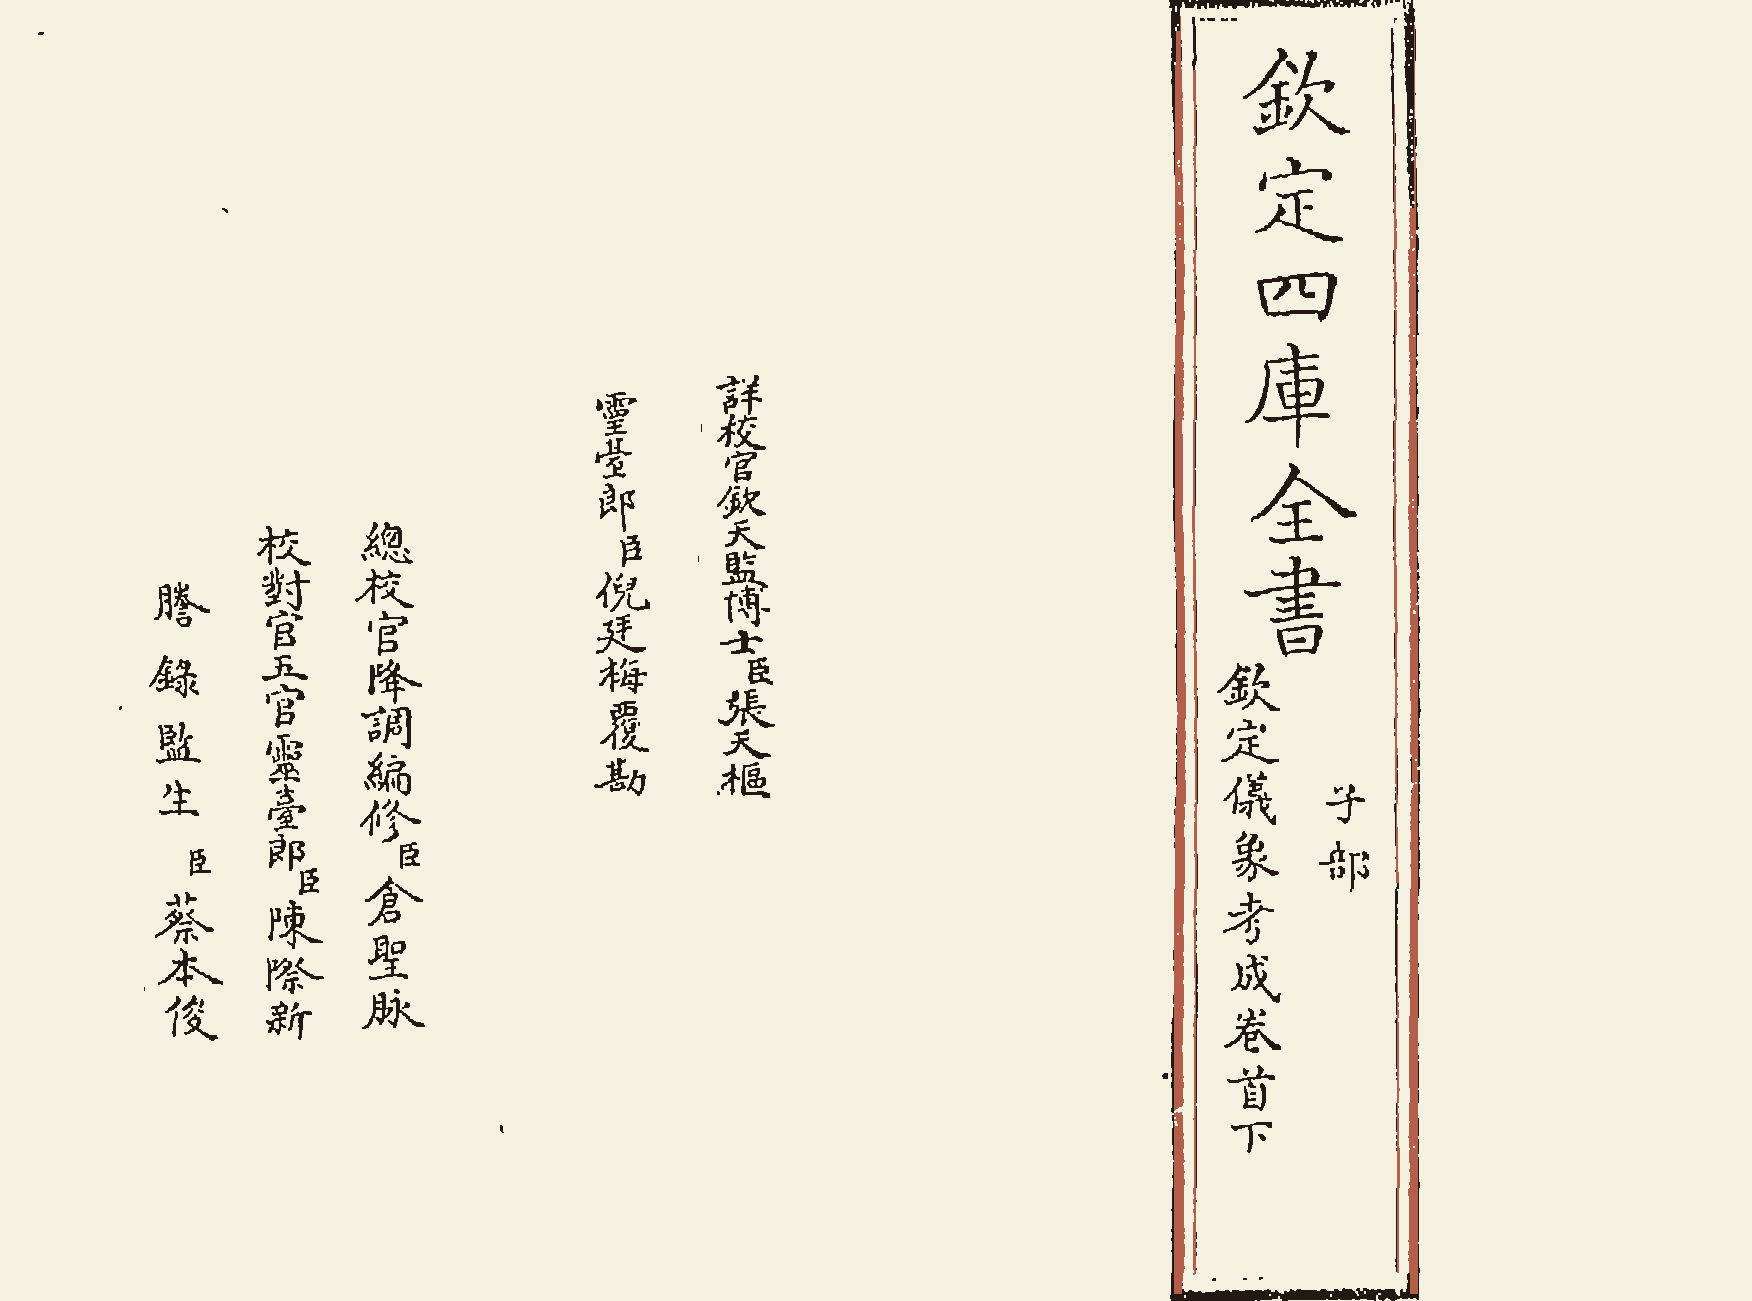
\includegraphics[width=\paperwidth,height=\paperheight,keepaspectratio]{img/0232.png}\clearpage
\begin{正文}
% ---- 册793 葉233 ----
\SetPageNumber{1}
欽定四庫全書\换行
欽定儀象考成卷首下\换行
御製璣衡撫辰儀説卷下\换行
　　用法\换行
　　算法\换行
\char"200B\relax\换行
\char"200B\relax\换行
\char"200B\relax\换行
\char"200B\relax\换行
\char"200B\relax\换行
\char"200B\relax\换行
\char"200B\relax\换行
\char"200B\relax\换行
\char"200B\relax\换行
\char"200B\relax\换行
\char"200B\relax
\par
% ---- 册793 葉236 ----
御製璣衡撫辰儀説卷下之一\换行
　用法\换行
　　測太陽時刻\换行
　　測日出入時刻及晝夜永短\换行
　　測太陽赤道緯度\换行
　　測午正太陽髙弧\换行
　　測太陽赤道經度\换行
　　測月星赤道經緯度\换行
　　測恒星求時刻\换行
　　測月五星求時刻\换行
　　測月星當中及偏度\换行
　　測月星出入地平時刻\换行
　　測南北真線\换行
　　測北極髙度\换行
　　測黄赤距度\换行
　　測黄白距度
\par
% ---- 册793 葉237 ----
　　測太陽時刻\换行
法以四遊圏東西推轉窺衡南北低昂令太陽從衡孔\换行
透光圓正或用薫黒玻璃置於下端衡孔視上端圓孔\换行
十字線正當太陽中心則窺衡與太陽參直乃視四遊\换行
圏下周指時度表臨於天常赤道之某時刻分即太陽\换行
時刻也若二分前後日影為赤道所礙則用窺衡上面\换行
立表測之\双列{\右小列{常時不為赤道所}\左小列{礙亦用此表為便}}若午正及卯酉前後日影\换行
為子午圏及龍柱所礙則用窺衡上面平行立表測之\换行
以四遊窺衡對凖太陽令上端表圓孔十字線影從下\换行
端表圓孔正中透出上端表直線影從下端表直縫正\换行
中透出\双列{\右小列{測時刻止用經度可止取直線影}\左小列{若測緯度則必取圓孔十字線影}}視指時度表\换行
所指即得太陽時刻若指時度表為子午圏所礙則易\换行
用借弧指時度表次用平行立表測定日影視借弧指\换行
時度表所指時刻加一小時即得太陽時刻盖借弧之\换行
長當遊旋赤道之十五度當天常赤道之一小時又借\换行
表在四遊圏之西所指時刻在本時前故加一小時即
\par
% ---- 册793 葉240 ----
為本時刻分也\换行
　　測日出入時刻及晝夜永短\换行
法於太陽出入地平時按前法測得太陽出入時刻乃\换行
計距午正前後若干刻分倍之即得晝刻計距子正前\换行
後若干刻分倍之即得夜刻\换行
　　測太陽赤道緯度\换行
法如前測凖太陽視窺衡下端指緯度表所指四遊圏\换行
右面距赤道度分即得太陽赤道緯度表指赤道北太\换行
陽緯度為在赤道南表指赤道南太陽緯度為在赤道\换行
北盖窺管以圓心為樞上端所窺在赤道北下端所指\换行
必在赤道南上端所窺在赤道南下端所指必在赤道\换行
北也\换行
　　測午正太陽髙弧\换行
法於午正時測得太陽赤道緯度在赤道北與赤道髙\换行
五十度五分相加在赤道南與赤道髙五十度五分相\换行
減即午正太陽髙弧也
\par
% ---- 册793 葉241 ----
　　測太陽赤道經度\换行
法用恒星作距測之取所知近午正前後一恒星\双列{\右小列{午正}\左小列{前後}}\换行
\双列{\右小列{取其𫎇氣少}\左小列{易得確凖也}}以其赤道經度之對衝用綰經度表於遊\换行
旋赤道綰定四遊圏\双列{\右小列{凡以儀器測星其上當星處為星}\左小列{之正位其下當人目處則星之對}}\换行
\双列{\右小列{冲故以星經度之對冲於}\左小列{遊旋赤道綰定四遊圏}}又任設一時用綰時度表於\换行
其時刻之對衝綰定天常赤道\双列{\右小列{天常環面乃日影所照}\左小列{之時其對冲則太陽所}}\换行
\双列{\右小列{臨之正位故於設時之對冲綰之如設丑正初}\左小列{刻則綰於未正初刻即太陽臨於丑正之位也}}乃将四\换行
逰圏帶定遊旋赤道用窺衡測凖距星隨之左旋𠉀至\换行
所設時刻\双列{\右小列{或鐘表或漏}\左小列{壺須得確凖}}視綰時度表對於遊旋赤道之\换行
某宫度分即太陽赤道經度也\双列{\右小列{環面時刻之對冲即太}\左小列{陽所臨之正位故其所}}\换行
\双列{\右小列{對遊旋赤道之宫}\左小列{度即太陽經度}}\换行
又法先以恒星作距測金星次以金星作距測太陽如\换行
金星晨見則於太陽未出之前取在金星西之一恒星\换行
作距以其赤道經度用平行線測經度表於遊旋赤道\换行
安定\双列{\右小列{三測皆係經度若距星之經度用對冲則測得之}\左小列{經度又須加減半周故距星不用對冲所測亦即}}\换行
\双列{\右小列{得本}\左小列{度也}}令一人用此平行線表窺定距星隨之左旋一人
\par
% ---- 册793 葉244 ----
用四遊窺衡測金星兩人同時測定乃視四遊圏指時\换行
度表所指遊旋赤道之宫度分即金星赤道經度次以\换行
金星赤道經度用平行線測經度表於遊旋赤道安定\换行
令一人窺定金星隨之左旋一人於太陽始出時用四\换行
遊窺衡測太陽乃視四遊圏指時度表所指遊旋赤道\换行
之宫度分即得太陽赤道經度若金星夕見則於太陽\换行
将入時任於某宫初度安定平行線測經度表令一人\换行
窺定金星又令一人用四遊窺衡測太陽視太陽距金\换行
星若干度記定俟太陽既入後取金星東之一恒星作\换行
距按前法測得金星赤道經度内減太陽距金星之度\换行
\双列{\右小列{星在東日}\左小列{在西故減}}即得太陽赤道經度也\双列{\右小列{太陽光大惟月及金}\左小列{星可以兩見然月有}}\换行
\双列{\右小列{視差不如用}\左小列{金星為凖也}}\换行
　　測月星赤道經緯度\换行
法於昏後曉前任設一時以本日太陽赤道經度與次\换行
日太陽赤道經度比例得本時太陽赤道經度\双列{\右小列{七政時}\左小列{憲書所}}\换行
\双列{\右小列{列乃子正之度子正後七政皆有行分故以本日子正}\左小列{之度分與次日子正之度分相減餘為一日十二時所}}
\par
% ---- 册793 葉245 ----
\双列{\右小列{行之分與設時距子正之時分為比例得設時距子}\左小列{正之行分加於本日子正之度分得本時之度分}}用\换行
綰時度表於遊旋赤道綰定又以所設時刻之對冲於\换行
天常赤道綰定𠉀至所設時刻用四遊窺衡測月星乃\换行
視指時度表所指遊旋赤道宫度加半周\双列{\右小列{環面時刻之}\左小列{對冲即為太}}\换行
\双列{\右小列{陽之正位環面之宮度却}\左小列{為月星之對冲故加半周}}即得所測月星赤道經度隨\换行
察指緯度表所指四遊圏距赤道南北度分即得所測\换行
月星赤道緯度也\双列{\右小列{緯之南北與前測}\左小列{太陽緯度法同}}\换行
又法用恒星作距測之以距星之赤道經度用平行線\换行
測經度表於遊旋赤道安定令一人用此平行線表窺\换行
定距星隨之左旋一人用四遊窺衡測月星兩人同時\换行
測定乃視指時度表所指遊旋赤道之度分即所測月\换行
星之赤道經度隨察指緯度表所指四遊圏之度分即\换行
得所測月星之赤道緯度也\换行
　　測恒星求時刻\换行
法先以恒星赤道經度用綰經度表於遊旋赤道綰定\换行
四遊圏次約計測時為某時依前法比例得本時太陽
\par
% ---- 册793 葉248 ----
赤道經度\双列{\右小列{太陽每日行一度於時為四分每一時行五}\左小列{分於時為二十秒故約計測量之時比例得}}\换行
\双列{\右小列{其時赤道經度即}\左小列{可用以測時刻也}}用綰時度表綰定遊旋赤道将四遊\换行
圏帶遊旋赤道推轉用窺衡測定恒星乃視綰時度表\换行
對於天常赤道之某時刻分加六時即太陽時刻也\双列{\右小列{天}\左小列{常}}\换行
\双列{\右小列{赤道之時刻乃日影對照之時故}\左小列{加六時始為太陽所臨之時刻也}}\换行
　　測月五星求時刻\换行
法以本時太陽赤道經度用綰時度表綰定遊旋赤道\换行
以月五星本時赤道經度之對冲用綰經度表於遊旋\换行
赤道綰定四遊圏将四遊圏帶遊旋赤道推轉用窺衡\换行
測定月星乃視綰時度表對於天常赤道之某時刻分\换行
加六時即得太陽時刻若太陽近子正前後綰時度表\换行
為子午圏所礙則向東或西借三十度綰定測之視所\换行
對時刻加減一時\双列{\右小列{向東借則加}\左小列{向西借則減}}即得太陽時刻若月五\换行
星近赤道或近午正前後為諸圏所礙則用窺管上面\换行
立表及平行立表測之與前測太陽時刻法同\换行
　　測月星當中及偏度
\par
% ---- 册793 葉249 ----
法以四遊窺衡隨時測月或星視指時度表當天常赤\换行
道之某時刻分記之\双列{\右小列{近午正則易用借弧}\左小列{指時度表加一小時}}午正為當中\换行
無偏度午正前為偏東午正後為偏西乃以距午時分\换行
變赤道度每一時為三十度每一小時為十五度每一\换行
分為十五分每一秒為十五秒共之為所偏度凡推月\换行
星當中及偏度者用此法測之則離合可辨凡有求時\换行
刻者用此法測定則時刻可推也\换行
　　測月星出入地平時刻\换行
法以本日子正月五星赤道經度或恒星經度之對冲\换行
用綰經度表於遊旋赤道綰定四遊圏又以本日子正\换行
太陽經度用綰時度表綰定遊旋赤道爰以四遊窺衡\换行
於月星出入地平時測之視綰時度表當天常赤道之\换行
某時刻分加六時為本日月星出入時刻之通數復計\换行
測時距本日子正後若干時刻比例得太陽行分變時\换行
\双列{\右小列{每一度為四分每十五分}\左小列{為一分每十五秒為一秒}}為太陽時差比例得月五星\换行
行分變時為月五星時差\双列{\右小列{恒星則無行}\左小列{分亦無時差}}乃於前所測月
\par
% ---- 册793 葉252 ----
星出入時刻之通數減太陽時差加月五星時差即得\换行
月星出入地平時刻盖日與月星測時皆用子正經度\换行
而子正後太陽有右旋之行分則時刻必差而早月五\换行
星亦有右旋之行分則時刻必差而遲\双列{\右小列{時刻左旋七政}\左小列{皆右旋太陽有}}\换行
\双列{\右小列{右旋之行分則測時太陽之經度必在所測時刻之前}\左小列{故差而早月五星有右旋之行分則測時月星之方位}}\换行
\双列{\右小列{必在所測時刻}\左小列{之後故差而遲}}故減太陽時差加月五星時差\双列{\右小列{若五星}\左小列{逆行則}}\换行
\双列{\右小列{時差}\左小列{亦減}}方為月星出入地平真時此與前測月星求時刻\换行
法同理設時可以預知故先求本時經度而後測月星\换行
出入難以懸定故先測而後加減時差其理相通其用\换行
尤便也\换行
　　測南北真線\换行
法於太陽出地平時測其距午東赤道度又於太陽入\换行
地平時測其距午西赤道度\双列{\右小列{測得太陽出入地平距午}\左小列{正前後若干時分變赤道}}\换行
\双列{\右小列{度即得距午正}\左小列{東西赤道度}}兩距午度相等則子午圏之向即南北\换行
真線若日出距午東之度多日入距午西之度少則子\换行
午圏之午正偏西若日出距午東之度少日入距午西
\par
% ---- 册793 葉253 ----
之度多則子午圏之午正偏東\双列{\右小列{此言午正乃子}\左小列{午圏之正南}}以兩測\换行
之距午度相減折半即所偏之赤道經度\双列{\右小列{若求地平偏}\左小列{度則用三角}}\换行
\双列{\右小列{法推之見算}\左小列{法第八則}}依所偏之度作線即南北真線也\换行
又法於冬至後測織女第一星昏刻此星當酉正之位\换行
以四遊圏安於酉正測其去極度若干\双列{\右小列{九十度内減赤}\左小列{道緯度餘即去}}\换行
\双列{\右小列{極}\左小列{度}}旦刻此星當卯正之位以四遊圏安於卯正測其去\换行
極度若干\双列{\右小列{織女星在赤道丑宫七度赤道北三十八度}\左小列{半冬至後半月内昏旦可以兩見故専取此}}\换行
\双列{\右小列{星測}\左小列{之}}兩去極度相等則子午圏之向即南北真線若卯\换行
正位測得去極度多酉正位測得去極度少則東逺西\换行
近即子午圈之北極偏西若卯正位測得去極度少酉\换行
正位測得去極度多則東近西逺即子午圈之北極偏\换行
東以兩測之去極度相減折半即所偏之赤道緯度\双列{\右小列{若}\左小列{求}}\换行
\双列{\右小列{地平偏度則用三角法}\左小列{推之見算法第十五則}}依所偏之度作線即南北真線\换行
也盖南北真線自北極過天頂平分赤道之地平上半\换行
周是為午正故向南測者以午正為凖向北測者以北\换行
極為凖太陽隨天左旋其出地入地距午必相等若其
\par
% ---- 册793 葉256 ----
不等必儀之午正偏也恒星繞地左旋其在東在西去\换行
極必相等若其不等必儀之北極偏也依其偏度正之\换行
則南北真線得矣又按渾儀經緯與天同象測太陽亦\换行
可用緯度測恒星亦可用經度然不及右二法之簡明\换行
推測精熟法理自見今不具悉也\换行
　　測北極髙度\换行
法於冬至前後以四遊圏安於正北測天權星\双列{\右小列{即北斗}\左小列{第四星}}\换行
昏刻此星在北極之下測其去極度若干旦刻此星在\换行
北極之上測其去極度若干\双列{\右小列{天權星今在赤道辰宫初}\左小列{度赤道北五十八度冬至}}\换行
\双列{\右小列{前後半月内昏旦可以}\左小列{兩見故専取此星測之}}兩去極度相等則儀之北極髙\换行
度與天合若在上之去極度少在下之去極度多則儀\换行
之北極差髙若在上之去極度多在下之去極度少則\换行
儀之北極差下以兩測之去極度相減折半即所差之\换行
地平緯度於儀之北極髙度加減之\双列{\右小列{差髙則減}\左小列{差下則加}}即天之\换行
北極髙度也盖天之北極無星故取大星之環繞北極\换行
上下者測之星之去極有定度則上下兩測之去極必
\par
% ---- 册793 葉257 ----
等若其不等則儀之髙下差也依其差度加減之則在\换行
天之北極髙度得矣又按舊法用地平緯儀測鉤陳大\换行
星以其在北極上下兩髙度相加折半得北極髙度取\换行
其距地髙無𫎇氣也今用渾儀測之則鉤陳大星為儀\换行
樞所礙須用借弧故取用天權星測其去極之較以備\换行
一例若以所測在北極上之去極度與所設北極髙度\换行
相加以所測在北極下之去極度與所設北極髙度相\换行
減得兩地平髙度相加折半得北極髙度與用鉤陳大\换行
星之理同\换行
　　測黄赤大距\换行
法於冬至日午正初刻測太陽在赤道南若干度分夏\换行
至日午正初刻測太陽在赤道北若干度分若冬至夏\换行
至皆在午正初刻則所測日距赤道南北之緯度即黄\换行
赤大距度若冬至夏至不正當午正則又用前測太陽\换行
赤道經度法測得太陽距冬夏至前後若干度分用有\换行
太陽赤道經緯度求黄赤交角之法\双列{\右小列{見算法}\左小列{第四則}}求得黄赤
\par
% ---- 册793 葉260 ----
交角即黄赤大距度也盖黄道與赤道斜交春秋分時\换行
太陽正當赤道春分後秋分前太陽在赤道北夏至而\换行
極北秋分後春分前太陽在赤道南冬至而極南故致\换行
日者必於冬夏二至今用弧線三角形法測得逐日之\换行
距緯皆可以推大距然春秋分前後黄道斜而緯差大\换行
以推大距其理𨼆而難知冬夏至前後黄道横而緯差\换行
微以推大距其象顯而易見故冬夏致日古今之通義\换行
也\换行
　　測黄白距限\双列{\右小列{距限即大距因大距又有大小故}\左小列{名距限以别之見數象考成後編}}\换行
法於春分日上弦秋分日下弦月距交九十度時測得\换行
月距赤道北若干度分春分日下弦秋分日上弦月距\换行
交九十度時測得月距赤道南若干度分與黄赤大距\换行
相減餘為黄白二道最大之距限又於冬至日望月距\换行
交九十度時測得月距赤道北若干度分夏至日望月\换行
距交九十度時測得月距赤道南若干度分與黄赤大\换行
距相減餘為黄白二道最小之距限盖白道與黄道斜
\par
% ---- 册793 葉261 ----
交月距交九十度則距黄道最逺故測黄白大距必於\换行
月距交九十度時然黄白大距與黄道成直角黄赤大\换行
距與赤道成直角惟冬夏二至黄道經圈與赤道經圈\换行
合為一線故測黄白大距又必於月當冬夏二至時\双列{\右小列{上}\左小列{編}}\换行
\双列{\右小列{専取月當夏至為其距地髙也}\左小列{若以對待而言則兼用冬夏至}}夫月距交九十度而又\换行
當冬夏二至則兩交必在春秋二分當是時而值兩弦\换行
則日必在春秋分而適當兩交值朔望則日必在冬夏\换行
至而距交九十度上編之法謂兩弦時交角大\双列{\右小列{交角之}\左小列{度即大}}\换行
\双列{\右小列{距}\左小列{度}}朔望時交角小後編之法謂日在兩交時交角大日\换行
距交九十度時交角小極二説之異致至此而得其合\换行
故測黄白大距必於春秋分兩弦冬夏至望日\双列{\右小列{朔日不}\左小列{見月故}}\换行
\双列{\右小列{惟用}\左小列{望日}}月距交九十度時測之春分之日上弦秋分之日\换行
下弦而月距交九十度是月當夏至而日在兩交也春\换行
分之日下弦秋分之日上弦而月距交九十度是月當\换行
冬至而日在兩交也以兩弦與日在兩交而論皆交角\换行
大冬至之日望而月距交九十度是月當夏至而日距
\par
% ---- 册793 葉264 ----
交九十度也夏至之日望而月距交九十度是月當冬\换行
至而日距交九十度也以朔望與日距交九十度而論\换行
皆交角小各測其距赤道度與黄赤大距相減則最大\换行
最小之黄白距限皆得矣按月行出黄道南為陽厯為\换行
正交\双列{\右小列{今為}\左小列{中交}}入黄道北為陰厯為中交\双列{\右小列{今為}\左小列{正交}}夏至在陰厯\换行
冬至在陽厯則月距赤道校黄道為逺故於所測距赤\换行
道度内減黄赤大距餘為黄白大距夏至在陽厯冬至\换行
在陰厯則月距赤道校黄道為近故於黄赤大距内減\换行
所測距赤道度餘為黄白大距又按古法黄白大距不\换行
逾六度弦望無殊故曰春秋致月今法交角有大小故\换行
又必兼於冬夏至測之也\换行
又法推得月離黄道冬夏至時預於前數刻或以太陽\换行
作距用綰時度表綰定時刻或以恒星作距用平行線\换行
測經度表對定距星皆以四遊圏指時度表對冬夏至\换行
宫度安定候月行至二至線上乃以窺衡測月距赤道\换行
南北緯度若干與黄赤大距相減餘為月距黄道南北
\par
% ---- 册793 葉265 ----
緯度以正交宫度與冬夏至宫度相減餘為月距正交\换行
黄道經度用有太陽赤道經緯度求黄赤交角之法\双列{\右小列{見}\左小列{算}}\换行
\双列{\右小列{法第}\左小列{四則}}求得交角度分即黄白距限盖月之緯度與黄道\换行
成直角其三角形之比例則黄道如赤道白道如黄道\换行
黄緯如赤緯黄白交角即如黄赤交角黄白大距即如\换行
黄赤大距也前法於分至弦望測月緯度乃測黄白大\换行
距正法然其時不易得此法於月離冬夏至時凡見月\换行
即可測叅之弦望與日距交之逺近則交角有大小之\换行
故亦可得而稽矣\换行
\char"200B\relax\换行
\char"200B\relax\换行
\char"200B\relax\换行
\char"200B\relax\换行
\char"200B\relax\换行
\char"200B\relax\换行
\char"200B\relax
\par
% ---- 册793 葉268 ----
御製璣衡撫辰儀説下之二\换行
　算法\换行
　　有太陽赤道緯度求午正髙弧\换行
　　有太陽視髙弧求午正晷影\换行
　　有太陽赤道緯度求赤道經度\换行
　　有太陽赤道經緯度求黄赤大距\换行
　　有太陽赤道緯度求黄道經度\换行
　　有太陽赤道緯度求出入地平及晝夜時刻\换行
　　有太陽赤道緯度求昏旦時刻\换行
　　有太陽赤道緯度求太陽出入地平偏度\双列{\右小列{二題}\左小列{}}\换行
　　有時刻有太陽赤道緯度求地平經緯度\换行
　　有節氣有太陽午正髙弧求交節氣時刻\换行
　　有日月星赤道經度求月星當中時刻\换行
　　有日月星赤道經度有時刻求月星當中及偏度\换行
　　有日月星赤道經緯度求月星出入地平時刻\换行
　　有月星赤道經緯度求黄道經緯度
\par
% ---- 册793 葉269 ----
　　有月星距午赤道度有赤道緯度求地平經緯度\换行
　　有二星赤道經緯度求二星斜距度\换行
　　有日月五星視髙度求實髙度\换行
\char"200B\relax\换行
\char"200B\relax\换行
\char"200B\relax\换行
\char"200B\relax\换行
\char"200B\relax\换行
\char"200B\relax\换行
\char"200B\relax\换行
\char"200B\relax\换行
\char"200B\relax\换行
\char"200B\relax\换行
\char"200B\relax\换行
\char"200B\relax\换行
\char"200B\relax
\par
\end{正文}\clearpage
\contentSetup{n-char-per-col = 20, n-column = 9}
\begin{正文}
\end{正文}
\嵌图{259.22pt}{211.13pt}{687.10pt}{283.77pt}{img/0272.png}
\begin{正文}
% ---- 册793 葉272 ----
\SetPageNumber{20}
設如北極出地三十九度五十五分午正初刻測得\换行
　太陽距赤道北十五度求髙弧幾何\换行
　　　　　　　　　　如圖甲為天頂甲乙丙丁\换行
　　　　　　　　　　為子午圏乙丙為地平丁\换行
　　　　　　　　　　為北極戊己為赤道丁丙\换行
　　　　　　　　　　為北極出地三十九度五\换行
　　　　　　　　　　十五分戊乙為赤道髙五\换行
　　　　　　　　　　十度五分庚為太陽庚戊\换行
　　　　　　　　　　為太陽距赤道北十五度\换行
　　　　　　　　　　庚乙為太陽髙弧太陽正\换行
　　　　　　　　　　當午正赤經與髙弧合則\换行
　　　　　　　　　　以庚戊距緯與戊乙赤道\换行
　　　　　　　　　　髙度相加得庚乙六十五\换行
　　　　　　　　　　度五分為午正太陽髙度\换行
　　　　　　　　　　若太陽距赤道南則以距\换行
　　　　　　　　　　緯與赤道髙度相減即午\换行
　　　　　　　　　　正太陽髙度也\换行
設如測得午正太陽髙弧四十度中表髙八尺求影
\par
\end{正文}\clearpage
\嵌图{211.28pt}{218.24pt}{643.91pt}{276.65pt}{img/0273.png}
\begin{正文}
% ---- 册793 葉273 ----
\SetPageNumber{21}
　長幾何\换行
　　　　　　　　　　法以半徑一千萬為一率\换行
　　　　　　　　　　午正太陽髙弧四十度之\换行
　　　　　　　　　　餘切一千一百九十一萬\换行
　　　　　　　　　　七千五百三十六為二率\换行
　　　　　　　　　　表髙八尺為三率求得四\换行
　　　　　　　　　　率九尺五寸三分四釐零\换行
　　　　　　　　　　二絲八忽八微為所求之\换行
　　　　　　　　　　影長也如圖甲乙為中表\换行
　　　　　　　　　　之髙丙為太陽丁為中影\换行
　　　　　　　　　　心甲丁乙角為午正太陽\换行
　　　　　　　　　　髙度乙丁為影長則以丁\换行
　　　　　　　　　　戊半徑與太陽髙弧餘切\换行
　　　　　　　　　　戊已之比同於甲乙表髙\换行
　　　　　　　　　　與乙丁影長之比也\换行
設如春分後測得太陽距赤道北十五度黄赤交角\换行
　二十三度二十九分求赤道經度幾何\换行
　　　　　　　　　　如圖甲乙丙丁為赤道甲
\par
\end{正文}\clearpage
\嵌图{171.14pt}{215.35pt}{820.73pt}{279.54pt}{img/0276.png}
\begin{正文}
% ---- 册793 葉276 ----
\SetPageNumber{22}
\插图页
　　　　　　　　　　戊丙己為黄道相交於甲\换行
　　　　　　　　　　丙甲為春分丙為秋分戊\换行
　　　　　　　　　　為夏至己為冬至庚為北\换行
　　　　　　　　　　極辛為南極庚戊乙辛己\换行
　　　　　　　　　　丁為過二極二至經圈乙\换行
　　　　　　　　　　至戊丁至己俱二十三度\换行
　　　　　　　　　　二十九分為黄赤大距即\换行
　　　　　　　　　　甲丙黄赤二道相交之角\换行
　　　　　　　　　　壬為太陽甲壬為太陽距\换行
\恢复丝栏
　　　　　　　　　　春分後黄道經度自庚辛\换行
　　　　　　　　　　南北二極過太陽壬作庚\换行
　　　　　　　　　　壬癸辛赤極經圏交赤道\换行
　　　　　　　　　　於癸癸點為太陽所當赤\换行
　　　　　　　　　　道宫度甲癸為太陽距春\换行
　　　　　　　　　　分後赤道經度壬癸為太\换行
　　　　　　　　　　陽距赤道北十五度法用\换行
　　　　　　　　　　甲壬癸正弧三角形有甲\换行
　　　　　　　　　　角黄赤交角有癸直角有
\par
\end{正文}\clearpage
\嵌图{176.39pt}{207.01pt}{769.93pt}{287.88pt}{img/0277.png}
\begin{正文}
% ---- 册793 葉277 ----
\SetPageNumber{23}
\插图页
　　　　　　　　　　壬癸距緯求甲癸赤道度\换行
　　　　　　　　　　以甲角二十三度二十九\换行
　　　　　　　　　　分之乙子正切四百三十\换行
　　　　　　　　　　四萬四千六百六十六為\换行
　　　　　　　　　　一率乙丑半徑一千萬為\换行
　　　　　　　　　　二率壬癸距緯十五度之\换行
　　　　　　　　　　癸寅正切二百六十七萬\换行
　　　　　　　　　　九千四百九十二為三率\换行
　　　　　　　　　　求得四率六百一十六萬\换行
\恢复丝栏
　　　　　　　　　　七千三百一十四為甲癸\换行
　　　　　　　　　　弧之正弦癸卯檢表得三\换行
　　　　　　　　　　十八度四分四十秒即甲\换行
　　　　　　　　　　癸太陽距春分後赤道經\换行
　　　　　　　　　　度與甲丁春分距冬至三\换行
　　　　　　　　　　宫相加得四宫八度四分\换行
　　　　　　　　　　四十秒即太陽赤道宫度\换行
　　　　　　　　　　也\换行
設如春分後測得太陽距赤道北十五度距春分後
\par
\end{正文}\clearpage
\嵌图{268.26pt}{209.25pt}{723.62pt}{285.65pt}{img/0280.png}
\begin{正文}
% ---- 册793 葉280 ----
\SetPageNumber{24}
　赤道經度三十八度四分四十秒求黄赤大距度\换行
　幾何\换行
　　　　　　　　　　如圖甲為春分甲角為黄\换行
　　　　　　　　　　赤交角當戊乙黄赤大距\换行
　　　　　　　　　　壬為太陽壬癸為太陽距\换行
　　　　　　　　　　赤道北十五度甲癸為太\换行
　　　　　　　　　　陽距春分後赤道經度三\换行
　　　　　　　　　　十八度四分四十秒用甲\换行
　　　　　　　　　　壬癸正弧三角形以甲癸\换行
　　　　　　　　　　赤道三十八度四分四十\换行
　　　　　　　　　　秒之癸卯正弦六百一十\换行
　　　　　　　　　　六萬七千三百一十四為\换行
　　　　　　　　　　一率壬癸距緯十五度之\换行
　　　　　　　　　　寅癸正切二百六十七萬\换行
　　　　　　　　　　九千四百九十二為二率\换行
　　　　　　　　　　乙丑半徑一千萬為三率\换行
　　　　　　　　　　求得四率四百三十四萬\换行
　　　　　　　　　　六千六百六十六為甲角
\par
\end{正文}\clearpage
\嵌图{598.94pt}{210.20pt}{392.93pt}{284.70pt}{img/0281.png}
\嵌图{144.29pt}{217.63pt}{132.27pt}{277.27pt}{img/0281_1.png}
\begin{正文}
% ---- 册793 葉281 ----
\SetPageNumber{25}
　　　　　　　　　　之正切乙子檢表得二十\换行
　　　　　　　　　　三度二十九分即甲角黄\换行
　　　　　　　　　　赤大距度也\换行
設如春分後測得太陽距赤道北十五度黄赤交角\换行
　二十三度二十九分求黄道經度幾何\换行
　　　　　　　　　　如圖甲為春分甲角為黄\换行
　　　　　　　　　　赤交角二十三度二十九\换行
　　　　　　　　　　分壬為太陽甲壬為太陽\换行
　　　　　　　　　　距春分後黄道經度壬癸\换行
　　　　　　　　　　為距赤道北十五度用甲\换行
　　　　　　　　　　壬癸正弧三角形有甲角\换行
　　　　　　　　　　黄赤交角有癸直角有壬\换行
　　　　　　　　　　癸距緯求甲壬黄道度以\换行
　　　　　　　　　　甲角二十三度二十九分\换行
　　　　　　　　　　之戊辰正弦三百九十八\换行
　　　　　　　　　　萬四千八百二十三為一\换行
　　　　　　　　　　率戊丑半徑一千萬為二\换行
　　　　　　　　　　率壬癸距緯十五度之壬
\par
\end{正文}\clearpage
\嵌图{723.65pt}{204.84pt}{268.22pt}{290.06pt}{img/0284.png}
\嵌图{167.32pt}{219.20pt}{382.61pt}{275.69pt}{img/0284_1.png}
\begin{正文}
% ---- 册793 葉284 ----
\SetPageNumber{26}
　　　　　　　　　　巳正弦二百五十八萬八\换行
　　　　　　　　　　千一百九十為三率求得\换行
　　　　　　　　　　四率六百四十九萬五千\换行
　　　　　　　　　　一百一十九為甲壬弧之\换行
　　　　　　　　　　正弦壬午檢表得四十度\换行
　　　　　　　　　　三十分十七秒即甲壬太\换行
　　　　　　　　　　陽距春分後黄道經度與\换行
　　　　　　　　　　甲已春分距冬至三宫相\换行
　　　　　　　　　　加得四宫十度三十分十\换行
　　　　　　　　　　七秒即太陽黄道宫度也\换行
設如北極出地三十九度五十五分測得太陽距赤\换行
　道北十五度求出入地平及晝夜時刻\换行
　　　　　　　　　　如圖甲為天頂甲乙丙丁\换行
　　　　　　　　　　為子午圏乙丙為地平丁\换行
　　　　　　　　　　為北極丁丙為北極出地\换行
　　　　　　　　　　三十九度五十五分戊己\换行
　　　　　　　　　　為赤道戊乙為赤道髙五\换行
　　　　　　　　　　十度零五分庚為太陽庚
\par
\end{正文}\clearpage
\嵌图{163.37pt}{218.18pt}{386.56pt}{276.72pt}{img/0285.png}
\begin{正文}
% ---- 册793 葉285 ----
\SetPageNumber{27}
　　　　　　　　　　辛為太陽距赤道北十五\换行
　　　　　　　　　　度壬為卯正酉正之位辛\换行
　　　　　　　　　　壬為日出入在卯前酉後\换行
　　　　　　　　　　赤道度用庚辛壬正弧三\换行
　　　　　　　　　　角形有辛直角有壬角赤\换行
　　　　　　　　　　道髙度有庚辛邊求辛壬\换行
　　　　　　　　　　邊以壬角五十度五分之\换行
　　　　　　　　　　正切一千一百九十五萬\换行
　　　　　　　　　　二千七百九十九為一率\换行
　　　　　　　　　　半徑一千萬為二率庚辛\换行
　　　　　　　　　　十五度之正切二百六十\换行
　　　　　　　　　　七萬九千四百九十二為\换行
　　　　　　　　　　三率求得四率二百二十\换行
　　　　　　　　　　四萬一千七百二十八為\换行
　　　　　　　　　　辛壬弧之正弦檢表得十\换行
　　　　　　　　　　二度五十七分十五秒即\换行
　　　　　　　　　　辛壬弧為日出入在卯前\换行
　　　　　　　　　　酉後赤道度變時得三刻
\par
\end{正文}\clearpage
\嵌图{171.14pt}{215.05pt}{820.73pt}{279.84pt}{img/0288.png}
\begin{正文}
% ---- 册793 葉288 ----
\SetPageNumber{28}
\插图页
　　　　　　　　　　六分四十九秒為卯前酉\换行
　　　　　　　　　　後分以減卯正得日出卯\换行
　　　　　　　　　　初初刻八分十一秒以加\换行
　　　　　　　　　　酉正得日入酉正三刻六\换行
　　　　　　　　　　分四十九秒復倍卯前酉\换行
　　　　　　　　　　後分得六刻十三分三十\换行
　　　　　　　　　　八秒與四十八刻相加得\换行
　　　　　　　　　　五十四刻十三分三十八\换行
　　　　　　　　　　秒為晝刻與四十八刻相\换行
\恢复丝栏
　　　　　　　　　　減得四十一刻一分二十\换行
　　　　　　　　　　二秒為夜刻也又法求己\换行
　　　　　　　　　　辛日出入距子正前後赤\换行
　　　　　　　　　　道度用丁丙庚正弧三角\换行
　　　　　　　　　　形有丙直角有丁丙北極\换行
　　　　　　　　　　出地度有丁庚日距北極\换行
　　　　　　　　　　度求丁角以丁庚七十五\换行
　　　　　　　　　　度之正切三千七百三十\换行
　　　　　　　　　　二萬零五百零八為一率
\par
\end{正文}\clearpage
\嵌图{612.78pt}{223.00pt}{379.10pt}{271.90pt}{img/0289.png}
\嵌图{163.01pt}{219.31pt}{386.92pt}{275.58pt}{img/0289_1.png}
\begin{正文}
% ---- 册793 葉289 ----
\SetPageNumber{29}
　　　　　　　　　　丁丙三十九度五十五分\换行
　　　　　　　　　　之正切八百三十六萬六\换行
　　　　　　　　　　千二百四十二為二率半\换行
　　　　　　　　　　徑一千萬為三率求得四\换行
　　　　　　　　　　率二百二十四萬一千七\换行
　　　　　　　　　　百二十八為丁角之餘弦\换行
　　　　　　　　　　檢表得七十七度二分四\换行
　　　　　　　　　　十五秒即辛已弧為日出\换行
　　　　　　　　　　入距子正前後赤道度變\换行
　　　　　　　　　　時得五小時零八分十一\换行
　　　　　　　　　　秒為日出入距子正前後\换行
　　　　　　　　　　分自子正起算為卯初初\换行
　　　　　　　　　　刻八分十一秒即日出時\换行
　　　　　　　　　　刻與二十四小時相減得\换行
　　　　　　　　　　酉正三刻六分四十九秒\换行
　　　　　　　　　　為日入時刻復倍日出入\换行
　　　　　　　　　　距子正前後分得四十一\换行
　　　　　　　　　　刻一分二十二秒為夜刻
\par
\end{正文}\clearpage
\嵌图{605.32pt}{212.83pt}{386.56pt}{282.06pt}{img/0292.png}
\begin{正文}
% ---- 册793 葉292 ----
\SetPageNumber{30}
　　　　　　　　　　與九十六刻相減餘五十\换行
　　　　　　　　　　四刻十三分三十八秒為\换行
　　　　　　　　　　晝刻也\换行
設如北極出地三十九度五十五分測得太陽距赤\换行
　道北十五度求昏旦時刻\换行
　　　　　　　　　　如圖甲為天頂甲乙丙丁\换行
　　　　　　　　　　為子午圈乙丙為地平丁\换行
　　　　　　　　　　為北極丁丙為北極出地\换行
　　　　　　　　　　三十九度五十五分甲丁\换行
\插图页
　　　　　　　　　　為北極距天頂五十度五\换行
　　　　　　　　　　分戊己為赤道庚為太陽\换行
　　　　　　　　　　庚辛為太陽距赤道北十\换行
　　　　　　　　　　五度丁庚為太陽距北極\换行
　　　　　　　　　　七十五度壬癸為太陽隨\换行
　　　　　　　　　　天西轉之赤道距等圈庚\换行
　　　　　　　　　　子為昏旦曚影限十八度\换行
　　　　　　　　　　甲庚為太陽距天頂一百\换行
　　　　　　　　　　零八度丑寅為地平下曚
\恢复丝栏
\par
\end{正文}\clearpage
\嵌图{171.43pt}{217.40pt}{820.44pt}{277.49pt}{img/0293.png}
\begin{正文}
% ---- 册793 葉293 ----
\SetPageNumber{31}
\插图页
　　　　　　　　　　影距等圈辛點為太陽所\换行
　　　　　　　　　　當昏旦時刻戊辛為太陽\换行
　　　　　　　　　　距午正前後赤道度用甲\换行
　　　　　　　　　　庚丁斜弧三角形有甲丁\换行
　　　　　　　　　　邊北極距天頂有丁庚邊\换行
　　　　　　　　　　日距北極有甲庚邊日距\换行
　　　　　　　　　　天頂求丁角距午赤道度\换行
　　　　　　　　　　以夾丁角之丁庚邊七十\换行
　　　　　　　　　　五度與甲丁邊五十度五\换行
\恢复丝栏
　　　　　　　　　　分相加得一百二十五度\换行
　　　　　　　　　　五分為總弧其餘弦五百\换行
　　　　　　　　　　七十四萬七千六百七十\换行
　　　　　　　　　　二又以甲丁丁庚二邊相\换行
　　　　　　　　　　減餘二十四度五十五分\换行
　　　　　　　　　　為較弧其餘弦九百零六\换行
　　　　　　　　　　萬九千二百一十五兩餘\换行
　　　　　　　　　　弦相加\双列{\右小列{總弧較弧一過象}\左小列{限一不過象限則}}\换行
　　　　　　　　　　\双列{\右小列{兩餘弦相加若兩弧俱不}\左小列{過象限或俱過象限則兩}}
\par
\end{正文}\clearpage
\嵌图{192.65pt}{215.83pt}{799.22pt}{279.06pt}{img/0296.png}
\begin{正文}
% ---- 册793 葉296 ----
\SetPageNumber{32}
\插图页
　　　　　　　　　　\双列{\右小列{餘弦}\左小列{相減}}得一千四百八十一\换行
　　　　　　　　　　萬六千八百八十七折半\换行
　　　　　　　　　　得七百四十萬零八千四\换行
　　　　　　　　　　百四十四為中數為一率\换行
　　　　　　　　　　以對丁角之甲庚邊一百\换行
　　　　　　　　　　零八度之大矢一千三百\换行
　　　　　　　　　　零九萬零一百七十\双列{\右小列{餘弦}\左小列{與半}}\换行
　　　　　　　　　　\双列{\右小列{徑相加}\左小列{得大矢}}與較弧二十四度\换行
　　　　　　　　　　五十五分之正矢\双列{\右小列{餘弦與}\左小列{半徑相}}\换行
\恢复丝栏
　　　　　　　　　　\双列{\右小列{減得}\左小列{正矢}}九百三十萬零七百\换行
　　　　　　　　　　八十五相減餘一千二百\换行
　　　　　　　　　　一十五萬九千三百八十\换行
　　　　　　　　　　五為矢較為二率半徑一\换行
　　　　　　　　　　千萬為三率求得四率一\换行
　　　　　　　　　　千六百四十一萬二千八\换行
　　　　　　　　　　百七十三為丁角之大矢\换行
　　　　　　　　　　\双列{\右小列{凡矢過於半徑者為}\左小列{大矢其角即為鈍角}}内減\换行
　　　　　　　　　　半徑一千萬餘六百四十
\par
\end{正文}\clearpage
\嵌图{182.48pt}{211.52pt}{809.40pt}{283.38pt}{img/0297.png}
\begin{正文}
% ---- 册793 葉297 ----
\SetPageNumber{33}
\插图页
　　　　　　　　　　一萬二千八百七十三為\换行
　　　　　　　　　　丁角之餘弦檢表得五十\换行
　　　　　　　　　　度六分四十四秒與半周\换行
　　　　　　　　　　相減餘一百二十九度五\换行
　　　　　　　　　　十三分十六秒為丁角度\换行
　　　　　　　　　　即旦刻太陽距午前昏刻\换行
　　　　　　　　　　太陽距午後赤道度變時\换行
　　　　　　　　　　得八小時二刻九分三十\换行
　　　　　　　　　　三秒與午正十二小時相\换行
\恢复丝栏
　　　　　　　　　　減得寅初一刻五分二十\换行
　　　　　　　　　　七秒即旦刻與午正十二\换行
　　　　　　　　　　小時相加得戌正二刻九\换行
　　　　　　　　　　分三十三秒即昏刻也如\换行
　　　　　　　　　　圖丁庚與丁甲相加得甲\换行
　　　　　　　　　　癸為總弧\双列{\右小列{丁庚丁癸丁壬}\左小列{三弧同為癸壬}}\换行
　　　　　　　　　　\双列{\右小列{距等圏所截}\左小列{故其度相等}}其正弦為癸\换行
　　　　　　　　　　卯餘弦為卯辰丁庚與丁\换行
　　　　　　　　　　甲相減餘甲壬為較弧其
\par
\end{正文}\clearpage
\嵌图{167.23pt}{203.63pt}{824.64pt}{291.26pt}{img/0300.png}
\begin{正文}
% ---- 册793 葉300 ----
\SetPageNumber{34}
\插图页
　　　　　　　　　　正弦為壬己餘弦為己辰\换行
　　　　　　　　　　以卯辰與己辰兩餘弦相\换行
　　　　　　　　　　加得巳卯折半得己午與\换行
　　　　　　　　　　未申等為中數又對丁角\换行
　　　　　　　　　　之甲庚邊與甲丑甲寅等\换行
　　　　　　　　　　其正弦為丑酉或寅酉餘\换行
　　　　　　　　　　弦為酉辰大矢為甲酉以\换行
　　　　　　　　　　甲酉與甲壬較弧之正矢\换行
　　　　　　　　　　甲已相減餘己酉與戌庚\换行
\恢复丝栏
　　　　　　　　　　等為矢較遂成壬庚戌與\换行
　　　　　　　　　　壬申未同式兩勾股形故\换行
　　　　　　　　　　未申與戌庚之比必同於\换行
　　　　　　　　　　壬申與壬庚之比也又戊\换行
　　　　　　　　　　辰為半徑壬申為距等圈\换行
　　　　　　　　　　之半徑壬庚與戊辛兩叚\换行
　　　　　　　　　　同為丁庚辛赤道經圏之\换行
　　　　　　　　　　所分則壬申與壬庚之比\换行
　　　　　　　　　　原同於戊辰與戊辛之比
\par
\end{正文}\clearpage
\嵌图{155.20pt}{208.44pt}{394.73pt}{286.46pt}{img/0301.png}
\begin{正文}
% ---- 册793 葉301 ----
\SetPageNumber{35}
\插图页
　　　　　　　　　　是以中數未申與矢較戌\换行
　　　　　　　　　　庚之比即同於半徑戊辰\换行
　　　　　　　　　　與丁角大矢戊辛之比也\换行
　　　　　　　　　　既得戊辛大矢内減戊辰\换行
　　　　　　　　　　半徑餘辛辰即丁外角餘\换行
　　　　　　　　　　弦檢表得丁外角所當辛\换行
　　　　　　　　　　巳弧之度復與半周相減\换行
　　　　　　　　　　即得丁角所當戊辛弧之\换行
　　　　　　　　　　度也\换行
\恢复丝栏
設如北極出地三十九度五十五分太陽出地平時\换行
　測得距赤道北十五度求地平偏度幾何\换行
　　　　　　　　　　如圖甲為天頂甲乙丙丁\换行
　　　　　　　　　　為子午圈乙丙為地平丁\换行
　　　　　　　　　　為北極丁丙為北極出地\换行
　　　　　　　　　　三十九度五十五分戊己\换行
　　　　　　　　　　為赤道庚為太陽庚辛為\换行
　　　　　　　　　　太陽距赤道北十五度壬\换行
　　　　　　　　　　為卯正庚壬為日出地平
\par
\end{正文}\clearpage
\嵌图{604.60pt}{218.75pt}{250.59pt}{276.15pt}{img/0304.png}
\嵌图{164.41pt}{215.08pt}{385.52pt}{279.82pt}{img/0304_1.png}
\begin{正文}
% ---- 册793 葉304 ----
\SetPageNumber{36}
　　　　　　　　　　偏度用庚辛壬正弧三角\换行
　　　　　　　　　　形有辛直角有壬角赤道\换行
　　　　　　　　　　髙度有庚辛邊求庚壬邊\换行
　　　　　　　　　　以壬角五十度五分之正\换行
　　　　　　　　　　弦七百六十六萬九千七\换行
　　　　　　　　　　百八十五為一率半徑一\换行
　　　　　　　　　　千萬為二率庚辛十五度\换行
　　　　　　　　　　之正弦二百五十八萬八\换行
　　　　　　　　　　千一百九十為三率求得\换行
　　　　　　　　　　四率三百三十七萬四千\换行
　　　　　　　　　　五百二十七為庚壬弧之\换行
　　　　　　　　　　正弦檢表得十九度四十\换行
　　　　　　　　　　三分十八秒為庚壬弧度\换行
　　　　　　　　　　即太陽出地平時正東偏\换行
　　　　　　　　　　北之度也\换行
設如北極出地三十九度五十五分太陽入地平時\换行
　測得距赤道南十五度求地平偏度㡬何\换行
　　　　　　　　　　如圖甲為天頂甲乙丙丁
\par
\end{正文}\clearpage
\嵌图{167.49pt}{205.29pt}{824.39pt}{289.61pt}{img/0305.png}
\begin{正文}
% ---- 册793 葉305 ----
\SetPageNumber{37}
\插图页
　　　　　　　　　　為子午圏乙丙為地平丁\换行
　　　　　　　　　　為北極丁丙為北極出地\换行
　　　　　　　　　　三十九度五十五分戊己\换行
　　　　　　　　　　為赤道庚為太陽庚辛為\换行
　　　　　　　　　　太陽距赤道南十五度壬\换行
　　　　　　　　　　為酉正庚壬為日入地平\换行
　　　　　　　　　　偏度用辛庚壬正弧三角\换行
　　　　　　　　　　形有辛直角有壬角赤道\换行
　　　　　　　　　　髙度有庚辛邊求庚壬邊\换行
\恢复丝栏
　　　　　　　　　　以壬角五十度五分之正\换行
　　　　　　　　　　弦七百六十六萬九千七\换行
　　　　　　　　　　百八十五為一率半徑一\换行
　　　　　　　　　　千萬為二率庚辛十五度\换行
　　　　　　　　　　之正弦二百五十八萬八\换行
　　　　　　　　　　千一百九十為三率求得\换行
　　　　　　　　　　四率三百三十七萬四千\换行
　　　　　　　　　　五百二十七為庚壬弧之\换行
　　　　　　　　　　正弦檢表得十九度四十
\par
\end{正文}\clearpage
\嵌图{597.14pt}{211.89pt}{394.73pt}{283.00pt}{img/0308.png}
\嵌图{147.59pt}{217.40pt}{128.97pt}{277.49pt}{img/0308_1.png}
\begin{正文}
% ---- 册793 葉308 ----
\SetPageNumber{38}
　　　　　　　　　　三分十八秒為庚壬弧度\换行
　　　　　　　　　　即太陽入地平時正西偏\换行
　　　　　　　　　　南之度也\换行
設如北極出地三十九度五十五分己正初刻測得\换行
　太陽距赤道北十五度求地平經緯度各㡬何\换行
　　　　　　　　　　如圖甲為天頂甲乙丙丁\换行
　　　　　　　　　　為子午圏乙丙為地平丁\换行
　　　　　　　　　　為北極戊己為赤道丁丙\换行
　　　　　　　　　　為北極出地三十九度五\换行
　　　　　　　　　　十五分甲丁為北極距天\换行
　　　　　　　　　　頂五十度五分庚為太陽\换行
　　　　　　　　　　庚辛為太陽距赤道北十\换行
　　　　　　　　　　五度丁庚為太陽距北極\换行
　　　　　　　　　　七十五度辛為己正初刻\换行
　　　　　　　　　　戊辛為太陽距午東赤道\换行
　　　　　　　　　　度三十度即丁角甲庚為\换行
　　　　　　　　　　太陽距天頂庚壬為太陽\换行
　　　　　　　　　　髙弧即地平緯度乙壬為
\par
\end{正文}\clearpage
\嵌图{171.14pt}{215.78pt}{820.73pt}{279.11pt}{img/0309.png}
\begin{正文}
% ---- 册793 葉309 ----
\SetPageNumber{39}
\插图页
　　　　　　　　　　太陽正南偏東地平經度\换行
　　　　　　　　　　即甲角之外角用甲丁庚\换行
　　　　　　　　　　斜弧三角形有丁角距午\换行
　　　　　　　　　　東赤道度有甲丁北極距\换行
　　　　　　　　　　天頂有丁庚太陽距北極\换行
　　　　　　　　　　求甲庚邊及甲角度乃自\换行
　　　　　　　　　　太陽庚點作庚癸垂弧於\换行
　　　　　　　　　　形外補成丁庚癸甲庚癸\换行
　　　　　　　　　　兩正弧三角形先用丁庚\换行
\恢复丝栏
　　　　　　　　　　癸形以半徑一千萬為一\换行
　　　　　　　　　　率丁角三十度之餘弦八\换行
　　　　　　　　　　百六十六萬零二百五十\换行
　　　　　　　　　　四為二率丁庚七十五度\换行
　　　　　　　　　　之正切三千七百三十二\换行
　　　　　　　　　　萬零五百零八為三率求\换行
　　　　　　　　　　得四率三千二百三十二\换行
　　　　　　　　　　萬零五百零八為丁癸弧\换行
　　　　　　　　　　之正切檢表得七十二度
\par
\end{正文}\clearpage
\嵌图{175.38pt}{210.18pt}{816.50pt}{284.72pt}{img/0312.png}
\begin{正文}
% ---- 册793 葉312 ----
\SetPageNumber{40}
\插图页
　　　　　　　　　　四十八分二十八秒即丁\换行
　　　　　　　　　　癸弧内減甲丁五十度五\换行
　　　　　　　　　　分餘二十二度四十三分\换行
　　　　　　　　　　二十八秒即甲癸弧又以\换行
　　　　　　　　　　半徑一千萬為一率丁角\换行
　　　　　　　　　　三十度之正切五百七十\换行
　　　　　　　　　　七萬三千五百零三為二\换行
　　　　　　　　　　率丁癸七十二度四十八\换行
　　　　　　　　　　分二十八秒之正弦九百\换行
\恢复丝栏
　　　　　　　　　　五十五萬三千一百八十\换行
　　　　　　　　　　四為三率求得四率五百\换行
　　　　　　　　　　五十一萬五千五百三十\换行
　　　　　　　　　　四為庚癸弧之正切次用\换行
　　　　　　　　　　甲庚癸形以甲癸二十二\换行
　　　　　　　　　　度四十三分二十八秒之\换行
　　　　　　　　　　正弦三百八十六萬二千\换行
　　　　　　　　　　九百九十六為一率前所\换行
　　　　　　　　　　得庚癸弧之正切五百五
\par
\end{正文}\clearpage
\嵌图{163.54pt}{209.93pt}{828.33pt}{284.96pt}{img/0313.png}
\begin{正文}
% ---- 册793 葉313 ----
\SetPageNumber{41}
\插图页
　　　　　　　　　　十一萬五千五百三十四\换行
　　　　　　　　　　為二率半徑一千萬為三\换行
　　　　　　　　　　率求得四率一千四百二\换行
　　　　　　　　　　十七萬七千八百六十六\换行
　　　　　　　　　　為甲角之正切檢表得五\换行
　　　　　　　　　　十四度五十九分三十五\换行
　　　　　　　　　　秒為甲角度即太陽正南\换行
　　　　　　　　　　偏東地平經度又以甲角\换行
　　　　　　　　　　五十四度五十九分三十\换行
\恢复丝栏
　　　　　　　　　　五秒之餘弦五百七十三\换行
　　　　　　　　　　萬六千七百五十六為一\换行
　　　　　　　　　　率半徑一千萬為二率甲\换行
　　　　　　　　　　癸二十二度四十三分二\换行
　　　　　　　　　　十八秒之正切四百一十\换行
　　　　　　　　　　八萬八千一百零四為三\换行
　　　　　　　　　　率求得四率七百三十萬\换行
　　　　　　　　　　零四百七十四為甲庚弧\换行
　　　　　　　　　　之正切檢表得三十六度
\par
\end{正文}\clearpage
\嵌图{167.36pt}{212.93pt}{824.52pt}{281.96pt}{img/0316.png}
\begin{正文}
% ---- 册793 葉316 ----
\SetPageNumber{42}
\插图页
　　　　　　　　　　七分五十二秒為甲庚弧\换行
　　　　　　　　　　即太陽距天頂之度與甲\换行
　　　　　　　　　　壬象限九十度相減餘庚\换行
　　　　　　　　　　壬五十三度五十二分八\换行
　　　　　　　　　　秒為太陽髙弧即地平緯\换行
　　　　　　　　　　度也\换行
　　　　　　　　　　又法自太陽庚點至卯正\换行
　　　　　　　　　　癸點作庚癸弧成庚辛癸\换行
　　　　　　　　　　庚壬癸兩正弧三角形算\换行
\恢复丝栏
　　　　　　　　　　之先用庚辛癸形以辛癸\换行
　　　　　　　　　　距卯正後赤道度六十度\换行
　　　　　　　　　　之正弦八百六十六萬零\换行
　　　　　　　　　　二百五十四為一率庚辛\换行
　　　　　　　　　　太陽距赤道北十五度之\换行
　　　　　　　　　　正切二百六十七萬九千\换行
　　　　　　　　　　四百九十二為二率半徑\换行
　　　　　　　　　　一千萬為三率求得四率\换行
　　　　　　　　　　三百零九萬四千零一十
\par
\end{正文}\clearpage
\嵌图{175.21pt}{210.99pt}{816.66pt}{283.90pt}{img/0317.png}
\begin{正文}
% ---- 册793 葉317 ----
\SetPageNumber{43}
\插图页
　　　　　　　　　　一為庚癸辛角之正切檢\换行
　　　　　　　　　　表得十七度十一分三十\换行
　　　　　　　　　　二秒即庚癸辛角與辛癸\换行
　　　　　　　　　　壬角五十度五分相加得\换行
　　　　　　　　　　六十七度十六分三十二\换行
　　　　　　　　　　秒即庚癸壬角又以庚癸\换行
　　　　　　　　　　辛角十七度十一分三十\换行
　　　　　　　　　　二秒之餘弦九百五十五\换行
　　　　　　　　　　萬三千一百八十四為一\换行
\恢复丝栏
　　　　　　　　　　率半徑一千萬為二率辛\换行
　　　　　　　　　　癸六十度之正切一千七\换行
　　　　　　　　　　百三十二萬零五百零八\换行
　　　　　　　　　　為三率求得四率一千八\换行
　　　　　　　　　　百一十三萬零六百一十\换行
　　　　　　　　　　三為庚癸弧之正切檢表\换行
　　　　　　　　　　得六十一度七分一十五\换行
　　　　　　　　　　秒為庚癸弧度次用庚壬\换行
　　　　　　　　　　癸形以半徑一千萬為一
\par
\end{正文}\clearpage
\嵌图{175.05pt}{204.37pt}{816.83pt}{290.52pt}{img/0320.png}
\begin{正文}
% ---- 册793 葉320 ----
\SetPageNumber{44}
\插图页
　　　　　　　　　　率庚癸壬角六十七度十\换行
　　　　　　　　　　六分三十二秒之餘弦三\换行
　　　　　　　　　　百八十六萬二千九百九\换行
　　　　　　　　　　十六為二率前所得庚癸\换行
　　　　　　　　　　弧之正切一千八百一十\换行
　　　　　　　　　　三萬零六百一十三為三\换行
　　　　　　　　　　率求得四率七百萬零三\换行
　　　　　　　　　　千八百四十九為壬癸弧\换行
　　　　　　　　　　之正切檢表得三十五度\换行
\恢复丝栏
　　　　　　　　　　零二十五秒即壬癸弧度\换行
　　　　　　　　　　與乙癸象限相減餘乙壬\换行
　　　　　　　　　　五十四度五十九分三十\换行
　　　　　　　　　　五秒即太陽正南偏東地\换行
　　　　　　　　　　平經度又以半徑一千萬\换行
　　　　　　　　　　為一率庚癸壬角六十七\换行
　　　　　　　　　　度十六分三十二秒之正\换行
　　　　　　　　　　弦九百二十二萬三千七\换行
　　　　　　　　　　百三十三為二率庚癸弧
\par
\end{正文}\clearpage
\嵌图{175.05pt}{216.39pt}{816.83pt}{278.50pt}{img/0321.png}
\begin{正文}
% ---- 册793 葉321 ----
\SetPageNumber{45}
\插图页
　　　　　　　　　　六十一度七分十五秒之\换行
　　　　　　　　　　正弦八百七十五萬六千\换行
　　　　　　　　　　四百零一為三率求得四\换行
　　　　　　　　　　率八百零七萬六千六百\换行
　　　　　　　　　　七十為庚壬弧之正弦檢\换行
　　　　　　　　　　表得五十三度五十二分\换行
　　　　　　　　　　七秒為庚壬太陽髙弧即\换行
　　　　　　　　　　地平緯度也\换行
　　　　　　　　　　又法用總較法算之以半\换行
\恢复丝栏
　　　　　　　　　　徑一千萬為一率丁角三\换行
　　　　　　　　　　十度之正矢\双列{\右小列{餘弦與半徑}\左小列{相減得正矢}}\换行
　　　　　　　　　　一百三十三萬九千七百\换行
　　　　　　　　　　四十六為二率以夾丁角\换行
　　　　　　　　　　之甲丁邊五十度五分與\换行
　　　　　　　　　　丁庚邊七十五度相加得\换行
　　　　　　　　　　一百二十五度五分為總\换行
　　　　　　　　　　弧其餘弦五百七十四萬\换行
　　　　　　　　　　七千六百七十二又以甲
\par
\end{正文}\clearpage
\嵌图{178.96pt}{217.35pt}{812.92pt}{277.55pt}{img/0324.png}
\begin{正文}
% ---- 册793 葉324 ----
\SetPageNumber{46}
\插图页
　　　　　　　　　　丁丁庚兩邊相減餘二十\换行
　　　　　　　　　　四度五十五分為較弧其\换行
　　　　　　　　　　餘弦九百零六萬九千二\换行
　　　　　　　　　　百一十五兩餘弦相加\双列{\右小列{總}\左小列{弧}}\换行
　　　　　　　　　　\双列{\右小列{過象限較弧不過象}\左小列{限故兩餘弦相加}}得一\换行
　　　　　　　　　　千四百八十一萬六千八\换行
　　　　　　　　　　百八十七折半得七百四\换行
　　　　　　　　　　十萬八千四百四十四為\换行
　　　　　　　　　　中數為三率求得四率九\换行
\恢复丝栏
　　　　　　　　　　十九萬二千五百四十三\换行
　　　　　　　　　　為矢較與較弧二十四度\换行
　　　　　　　　　　五十五分之正矢九十三\换行
　　　　　　　　　　萬零七百八十五相加得\换行
　　　　　　　　　　一百九十二萬三千三百\换行
　　　　　　　　　　二十八為甲庚對邊之正\换行
　　　　　　　　　　矢與半徑一千萬相減餘\换行
　　　　　　　　　　八百零七萬六千六百七\换行
　　　　　　　　　　十二為甲庚弧之餘弦檢
\par
\end{正文}\clearpage
\嵌图{178.96pt}{222.08pt}{812.92pt}{272.82pt}{img/0325.png}
\begin{正文}
% ---- 册793 葉325 ----
\SetPageNumber{47}
\插图页
　　　　　　　　　　表得三十六度七分五十\换行
　　　　　　　　　　三秒為甲庚太陽距天頂\换行
　　　　　　　　　　度與甲壬象限相減餘五\换行
　　　　　　　　　　十三度五十二分七秒為\换行
　　　　　　　　　　庚壬太陽髙弧即地平緯\换行
　　　　　　　　　　度也如圖戊癸為半徑戊\换行
　　　　　　　　　　辛為丁角之正矢甲丁與\换行
　　　　　　　　　　丁庚相加得甲子為總弧\换行
　　　　　　　　　　\双列{\右小列{丁庚丁子丁寅三弧同為}\左小列{子寅距等圏所截故其度}}\换行
\恢复丝栏
　　　　　　　　　　\双列{\右小列{相}\左小列{等}}其正弦為子丑餘弦為\换行
　　　　　　　　　　癸丑甲丁與丁庚相減得\换行
　　　　　　　　　　甲寅為較弧其正弦為寅\换行
　　　　　　　　　　卯餘弦為癸卯兩餘弦相\换行
　　　　　　　　　　加得卯丑折半得卯辰與\换行
　　　　　　　　　　巳午等為中數又對丁角\换行
　　　　　　　　　　之甲庚邊與甲未等其正\换行
　　　　　　　　　　弦為未申餘弦為申癸正\换行
　　　　　　　　　　矢為甲申以甲申與甲寅
\par
\end{正文}\clearpage
\嵌图{178.96pt}{214.59pt}{812.92pt}{280.30pt}{img/0328.png}
\begin{正文}
% ---- 册793 葉328 ----
\SetPageNumber{48}
\插图页
　　　　　　　　　　較弧之正矢甲卯相減餘\换行
　　　　　　　　　　卯申與酉庚等為矢較遂\换行
　　　　　　　　　　成寅午巳寅庚酉同式兩\换行
　　　　　　　　　　勾股形而寅午與寅庚之\换行
　　　　　　　　　　比同於已午與酉庚之比\换行
　　　　　　　　　　又寅午為子寅距等圏之\换行
　　　　　　　　　　半徑寅庚與戊辛兩叚同\换行
　　　　　　　　　　為丁庚辛過赤極經圏之\换行
　　　　　　　　　　所分則寅午與寅庚之比\换行
\恢复丝栏
　　　　　　　　　　原同於戊癸與戊辛之比\换行
　　　　　　　　　　是以半徑戊癸與丁角正\换行
　　　　　　　　　　矢戊辛之比即同於中數\换行
　　　　　　　　　　巳午與酉庚之比而酉庚\换行
　　　　　　　　　　與卯申矢較等既得卯申\换行
　　　　　　　　　　矢較與甲寅較弧之正矢\换行
　　　　　　　　　　甲卯相加得甲申即為甲\换行
　　　　　　　　　　庚弧之正矢與甲癸半徑\换行
　　　　　　　　　　相減餘癸申為甲庚弧之
\par
\end{正文}\clearpage
\嵌图{176.39pt}{213.78pt}{769.93pt}{281.11pt}{img/0329.png}
\begin{正文}
% ---- 册793 葉329 ----
\SetPageNumber{49}
\插图页
　　　　　　　　　　餘弦檢表得甲庚弧之度\换行
　　　　　　　　　　與甲壬象限相減餘庚壬\换行
　　　　　　　　　　弧即太陽髙弧之度也次\换行
　　　　　　　　　　求甲角則以甲庚弧三十\换行
　　　　　　　　　　六度七分五十三秒之正\换行
　　　　　　　　　　弦五百八十九萬六千三\换行
　　　　　　　　　　百八十九為一率丁庚弧\换行
　　　　　　　　　　七十五度之正弦九百六\换行
　　　　　　　　　　十五萬九千二百五十八\换行
\恢复丝栏
　　　　　　　　　　為二率丁角三十度之正\换行
　　　　　　　　　　弦五百萬為三率求得四\换行
　　　　　　　　　　率八百一十九萬零八百\换行
　　　　　　　　　　二十五為甲外角之正弦\换行
　　　　　　　　　　檢表得五十四度五十九\换行
　　　　　　　　　　分三十五秒為甲外角度\换行
　　　　　　　　　　即太陽正南偏東之地平\换行
　　　　　　　　　　經度也\换行
設如北極出地三十九度五十五分春分日測得午
\par
\end{正文}\clearpage
\嵌图{229.36pt}{216.00pt}{762.52pt}{278.90pt}{img/0332.png}
\begin{正文}
% ---- 册793 葉332 ----
\SetPageNumber{50}
　正太陽髙五十度求春分時刻\换行
　　　　　　　　　　法先以午正太陽視髙五\换行
　　　　　　　　　　十度減𫎇氣差五十秒加\换行
　　　　　　　　　　地半徑差六秒得午正太\换行
　　　　　　　　　　陽實髙四十九度五十九\换行
　　　　　　　　　　分十六秒與赤道髙五十\换行
　　　　　　　　　　度五分相減餘五分四十\换行
　　　　　　　　　　四秒為太陽距赤道南之\换行
　　　　　　　　　　緯度即知春分在午正東\换行
　　　　　　　　　　春分時刻在午正後也如\换行
　　　　　　　　　　圖甲為天頂甲乙丙丁為\换行
　　　　　　　　　　子午圏乙丙為地平丁為\换行
　　　　　　　　　　北極丁丙為北極出地三\换行
　　　　　　　　　　十九度五十五分戊已為\换行
　　　　　　　　　　赤道戊乙為赤道髙五十\换行
　　　　　　　　　　度五分庚為太陽庚乙為\换行
　　　　　　　　　　午正太陽實髙四十九度\换行
　　　　　　　　　　五十九分十六秒庚戊為
\par
\end{正文}\clearpage
\嵌图{178.78pt}{217.04pt}{813.10pt}{277.86pt}{img/0333.png}
\begin{正文}
% ---- 册793 葉333 ----
\SetPageNumber{51}
\插图页
　　　　　　　　　　太陽距赤道南五分四十\换行
　　　　　　　　　　四秒爰用庚戊辛正弧三\换行
　　　　　　　　　　角形有戊直角有辛角黄\换行
　　　　　　　　　　赤交角有庚戊距緯求庚\换行
　　　　　　　　　　辛太陽距春分黄道度以\换行
　　　　　　　　　　辛角二十三度二十九分\换行
　　　　　　　　　　之正弦三百九十八萬四\换行
　　　　　　　　　　千八百二十三為一率半\换行
　　　　　　　　　　徑一千萬為二率庚戊五\换行
\恢复丝栏
　　　　　　　　　　分四十四秒之正弦一萬\换行
　　　　　　　　　　六千六百七十七為三率\换行
　　　　　　　　　　求得四率四萬一千八百\换行
　　　　　　　　　　五十一為庚辛弧之正弦\换行
　　　　　　　　　　檢表得十四分二十三秒\换行
　　　　　　　　　　十五微為太陽距春分黄\换行
　　　　　　　　　　道度乃以一日之日平行\换行
　　　　　　　　　　五十九分八秒二十微為\换行
　　　　　　　　　　一率\双列{\右小列{二分時太陽之實行}\左小列{與平行相近故即用}}
\par
\end{正文}\clearpage
\嵌图{726.11pt}{202.96pt}{265.76pt}{291.94pt}{img/0336.png}
\嵌图{159.10pt}{206.65pt}{390.83pt}{288.25pt}{img/0336_1.png}
\begin{正文}
% ---- 册793 葉336 ----
\SetPageNumber{52}
　　　　　　　　　　\双列{\右小列{平行為一率若他節氣須}\左小列{用本日之實行為一率}}\换行
　　　　　　　　　　周日一千四百四十分為\换行
　　　　　　　　　　二率太陽距春分黄道度\换行
　　　　　　　　　　十四分二十三秒十五微\换行
　　　　　　　　　　為三率求得四率三百五\换行
　　　　　　　　　　十分十九秒四十微以六\换行
　　　　　　　　　　十分收之得五時五十分\换行
　　　　　　　　　　十九秒四十微為春分距\换行
　　　　　　　　　　午正後之時刻即酉初三\换行
　　　　　　　　　　刻五分十九秒四十微也\换行
設如太陽赤道經度為戌官十五度木星赤道經度\换行
　為午宫初度求木星當中之時刻\双列{\右小列{月恒}\左小列{星同}}\换行
　　　　　　　　　　如圖甲為天頂甲乙丙丁\换行
　　　　　　　　　　為子午圏乙丙為地平丁\换行
　　　　　　　　　　為北極戊已為赤道庚辛\换行
　　　　　　　　　　為黄道戊點為木星所當\换行
　　　　　　　　　　赤道之午宫初度亦即正\换行
　　　　　　　　　　午赤道經度壬為太陽當
\par
\end{正文}\clearpage
\嵌图{730.02pt}{209.89pt}{261.85pt}{285.00pt}{img/0337.png}
\嵌图{155.20pt}{211.74pt}{394.73pt}{283.15pt}{img/0337_1.png}
\begin{正文}
% ---- 册793 葉337 ----
\SetPageNumber{53}
　　　　　　　　　　赤道之癸為戌宫十五度\换行
　　　　　　　　　　則於正午戊點赤道經度\换行
　　　　　　　　　　午宫初度内減癸點太陽\换行
　　　　　　　　　　赤道經度戌宫十五度餘\换行
　　　　　　　　　　戊癸三宫十五度為太陽\换行
　　　　　　　　　　距午西赤道度變時得七\换行
　　　　　　　　　　小時自午正初刻起算得\换行
　　　　　　　　　　戌初初刻即木星當中之\换行
　　　　　　　　　　時刻也\换行
設如亥初初刻測得太陽赤道經度為戌宫十五度\换行
　太陰赤道經度為巳宫初度求太陰當中及偏度\换行
　\双列{\右小列{五星恒}\左小列{星同}}\换行
　　　　　　　　　　如圖甲為天頂甲乙丙丁\换行
　　　　　　　　　　為子午圏乙丙為地平丁\换行
　　　　　　　　　　為北極戊已為赤道庚辛\换行
　　　　　　　　　　為黄道壬為太陽當赤道\换行
　　　　　　　　　　之癸為戌宫十五度戊為\换行
　　　　　　　　　　正午之位癸為亥初初刻
\par
\end{正文}\clearpage
\嵌图{151.29pt}{211.67pt}{398.64pt}{283.22pt}{img/0340.png}
\begin{正文}
% ---- 册793 葉340 ----
\SetPageNumber{54}
\插图页
　　　　　　　　　　距正午九小時變赤道度\换行
　　　　　　　　　　得戊癸太陽距午西赤道\换行
　　　　　　　　　　度四宫十五度與癸點太\换行
　　　　　　　　　　陽赤道經度戌宫十五度\换行
　　　　　　　　　　相加得巳宫初度為正午\换行
　　　　　　　　　　戊點赤道經度與太陰赤\换行
　　　　　　　　　　道經度相合即為亥初初\换行
　　　　　　　　　　刻太陰當中如太陰赤道\换行
　　　　　　　　　　經度大於正午赤道經度\换行
\恢复丝栏
　　　　　　　　　　為偏東小於正午赤道經\换行
　　　　　　　　　　度為偏西也\换行
設如北極出地三十九度五十五分本日子正初刻\换行
　太陽赤道經度為戌宫十五度太陰赤道經度為\换行
　申宫初度距赤道北十八度至次日子正初刻太\换行
　陽赤道經度為戌宫十六度太陰赤道經度為申\换行
　宫十三度求太陰入地平時刻\双列{\右小列{太陰出地倣此}\左小列{五星恒星並同}}\换行
　　　　　　　　　　如圖甲為天頂甲乙丙丁\换行
　　　　　　　　　　為子午圏乙丙為地平丁
\par
\end{正文}\clearpage
\嵌图{175.05pt}{212.33pt}{816.83pt}{282.57pt}{img/0341.png}
\begin{正文}
% ---- 册793 葉341 ----
\SetPageNumber{55}
\插图页
　　　　　　　　　　為北極丁丙為北極出地\换行
　　　　　　　　　　三十九度五十五分戊已\换行
　　　　　　　　　　為赤道戊乙為赤道髙五\换行
　　　　　　　　　　十度五分庚辛為黄道本\换行
　　　　　　　　　　日子正初刻太陽在壬當\换行
　　　　　　　　　　赤道之癸為戌宫十五度\换行
　　　　　　　　　　太陰在子當赤道之丑為\换行
　　　　　　　　　　申宫初度丑癸為太陰距\换行
　　　　　　　　　　太陽四十五度子丑為太\换行
\恢复丝栏
　　　　　　　　　　陰距赤道北十八度寅為\换行
　　　　　　　　　　酉正之位丑寅為太陰入\换行
　　　　　　　　　　地在酉正後赤道度用子\换行
　　　　　　　　　　丑寅正弧三角形有丑直\换行
　　　　　　　　　　角有寅角有子丑邊求丑\换行
　　　　　　　　　　寅邊以寅角五十度五分\换行
　　　　　　　　　　之正切一千一百九十五\换行
　　　　　　　　　　萬二千七百九十九為一\换行
　　　　　　　　　　率半徑一千萬為二率子
\par
\end{正文}\clearpage
\嵌图{167.23pt}{213.56pt}{824.64pt}{281.33pt}{img/0344.png}
\begin{正文}
% ---- 册793 葉344 ----
\SetPageNumber{56}
\插图页
　　　　　　　　　　丑十八度之正切三百二\换行
　　　　　　　　　　十四萬九千一百九十七\换行
　　　　　　　　　　為三率求得四率二百七\换行
　　　　　　　　　　十一萬八千三百五十七\换行
　　　　　　　　　　為丑寅弧之正弦檢表得\换行
　　　　　　　　　　十五度四十六分二十五\换行
　　　　　　　　　　秒為丑寅太陰入地在酉\换行
　　　　　　　　　　正後赤道度與丑癸太陰\换行
　　　　　　　　　　距太陽四十五度相加得\换行
\恢复丝栏
　　　　　　　　　　寅癸六十度四十六分二\换行
　　　　　　　　　　十五秒為太陽距酉正後\换行
　　　　　　　　　　赤道度變時得四小時三\换行
　　　　　　　　　　分六秒加酉正十八小時\换行
　　　　　　　　　　得二十二小時三分六秒\换行
　　　　　　　　　　為本日太陰入地時刻之\换行
　　　　　　　　　　通數復以本日次日子正\换行
　　　　　　　　　　初刻太陽赤道經度相減\换行
　　　　　　　　　　得一度為一日之日行度
\par
\end{正文}\clearpage
\嵌图{167.23pt}{205.27pt}{824.64pt}{289.62pt}{img/0345.png}
\begin{正文}
% ---- 册793 葉345 ----
\SetPageNumber{57}
\插图页
　　　　　　　　　　以通數距子正後之時分\换行
　　　　　　　　　　為比例得太陽行分為五\换行
　　　　　　　　　　十五分八秒變時得三分\换行
　　　　　　　　　　四十一秒為太陽時差以\换行
　　　　　　　　　　本日次日子正初刻太陰\换行
　　　　　　　　　　赤道經度相減得十三度\换行
　　　　　　　　　　為一日之月行度以通數\换行
　　　　　　　　　　距子正後之時分為比例\换行
　　　　　　　　　　得太陰行分為十一度五\换行
\恢复丝栏
　　　　　　　　　　十六分四十一秒變時得\换行
　　　　　　　　　　四十七分四十七秒為太\换行
　　　　　　　　　　陰時差乃於本日太陰入\换行
　　　　　　　　　　地時刻之通數二十二小\换行
　　　　　　　　　　時三分六秒内減太陽時\换行
　　　　　　　　　　差三分四十一秒加太陰\换行
　　　　　　　　　　時差四十七分四十七秒\换行
　　　　　　　　　　得二十二小時四十七分\换行
　　　　　　　　　　十二秒自子正後計之為
\par
\end{正文}\clearpage
\嵌图{175.05pt}{219.35pt}{816.83pt}{275.55pt}{img/0348.png}
\begin{正文}
% ---- 册793 葉348 ----
\SetPageNumber{58}
\插图页
　　　　　　　　　　亥正三刻二分十二秒即\换行
　　　　　　　　　　太陰入地平之時刻也盖\换行
　　　　　　　　　　太陰入地時刻之通數乃\换行
　　　　　　　　　　以本日子正初刻之赤道\换行
　　　　　　　　　　經度立算然太陰入地在\换行
　　　　　　　　　　子正後太陽太陰俱有右\换行
　　　　　　　　　　旋之行分太陽右旋則其\换行
　　　　　　　　　　赤經已過癸點之東時刻\换行
　　　　　　　　　　必差而早太陰右旋則其\换行
\恢复丝栏
　　　　　　　　　　赤經亦過丑點之東及隨\换行
　　　　　　　　　　天西轉以至入地時刻必\换行
　　　　　　　　　　差而遲且太陽行分少太\换行
　　　　　　　　　　陰行分多是太陽當癸點\换行
　　　　　　　　　　之時太陰尚在地平上逮\换行
　　　　　　　　　　太陰入地太陽赤經必又\换行
　　　　　　　　　　在癸點之西故於通數内\换行
　　　　　　　　　　減太陽時差加太陰時差\换行
　　　　　　　　　　方為太陰入地之時刻也
\par
\end{正文}\clearpage
\嵌图{307.93pt}{213.51pt}{683.94pt}{281.38pt}{img/0349.png}
\begin{正文}
% ---- 册793 葉349 ----
\SetPageNumber{59}
設如黄赤大距二十三度二十九分測得大角星赤\换行
　道經度卯宫一度七分二十六秒赤道緯北二十\换行
　度三十分四十二秒求黄道經緯度幾何\双列{\右小列{月五}\左小列{星同}}\换行
　　　　　　　　　　如圖甲為赤極乙為黄極\换行
　　　　　　　　　　甲乙為黄赤二極相距二\换行
　　　　　　　　　　十三度二十九分丙為大\换行
　　　　　　　　　　角星丁戊為赤道已庚為\换行
　　　　　　　　　　黄道辛點為赤道經度卯\换行
　　　　　　　　　　宫一度七分二十六秒丁\换行
　　　　　　　　　　辛為距冬至前赤道經度\换行
　　　　　　　　　　五十八度五十二分三十\换行
　　　　　　　　　　四秒即甲角丙辛為赤道\换行
　　　　　　　　　　緯北二十度三十分四十\换行
　　　　　　　　　　二秒甲丙為星距赤極六\换行
　　　　　　　　　　十九度二十九分十八秒\换行
　　　　　　　　　　壬點為黄道經度己壬為\换行
　　　　　　　　　　距冬至前黄道經度即乙\换行
　　　　　　　　　　角之外角丙壬為黄道北
\par
\end{正文}\clearpage
\嵌图{167.23pt}{207.38pt}{824.64pt}{287.52pt}{img/0352.png}
\begin{正文}
% ---- 册793 葉352 ----
\SetPageNumber{60}
\插图页
　　　　　　　　　　緯度乙丙為星距黄極度\换行
　　　　　　　　　　用甲乙丙斜弧三角形有\换行
　　　　　　　　　　甲角及甲乙甲丙二邊求\换行
　　　　　　　　　　乙角及乙丙邊先求乙角\换行
　　　　　　　　　　自大角星丙點作丙癸垂\换行
　　　　　　　　　　弧於形外補成甲丙癸乙\换行
　　　　　　　　　　丙癸兩正弧三角形先用\换行
　　　　　　　　　　甲丙癸形以半徑一千萬\换行
　　　　　　　　　　為一率甲角五十八度五\换行
\恢复丝栏
　　　　　　　　　　十二分三十四秒之餘弦\换行
　　　　　　　　　　五百一十六萬八千九百\换行
　　　　　　　　　　零三為二率甲丙六十九\换行
　　　　　　　　　　度二十九分十八秒之正\换行
　　　　　　　　　　切二千六百七十二萬九\换行
　　　　　　　　　　千六百一十六為三率求\换行
　　　　　　　　　　得四率一千三百八十一\换行
　　　　　　　　　　萬六千二百七十九為甲\换行
　　　　　　　　　　癸弧之正切檢表得五十
\par
\end{正文}\clearpage
\嵌图{175.05pt}{209.87pt}{816.83pt}{285.02pt}{img/0353.png}
\begin{正文}
% ---- 册793 葉353 ----
\SetPageNumber{61}
\插图页
　　　　　　　　　　四度六分十三秒為甲癸\换行
　　　　　　　　　　弧内減甲乙弧二十三度\换行
　　　　　　　　　　二十九分餘三十度三十\换行
　　　　　　　　　　七分十三秒為乙癸弧又\换行
　　　　　　　　　　以半徑一千萬為一率甲\换行
　　　　　　　　　　角五十八度五十二分三\换行
　　　　　　　　　　十四秒之正切一千六百\换行
　　　　　　　　　　五十六萬一千五百七十\换行
　　　　　　　　　　三為二率甲癸五十四度\换行
\恢复丝栏
　　　　　　　　　　六分十三秒之正弦八百\换行
　　　　　　　　　　一十萬零七百八十六為\换行
　　　　　　　　　　三率求得四率一千三百\换行
　　　　　　　　　　四十一萬六千一百七十\换行
　　　　　　　　　　六為丙癸弧之正切次用\换行
　　　　　　　　　　乙丙癸形以乙癸弧三十\换行
　　　　　　　　　　度三十七分十三秒之正\换行
　　　　　　　　　　弦五百零九萬三千四百\换行
　　　　　　　　　　六十為一率前所得丙癸
\par
\end{正文}\clearpage
\嵌图{167.23pt}{206.21pt}{824.64pt}{288.68pt}{img/0356.png}
\begin{正文}
% ---- 册793 葉356 ----
\SetPageNumber{62}
\插图页
　　　　　　　　　　弧之正切一千三百四十\换行
　　　　　　　　　　一萬六千一百七十六為\换行
　　　　　　　　　　二率半徑一千萬為三率\换行
　　　　　　　　　　求得四率二千六百三十\换行
　　　　　　　　　　四萬零五為乙角之正切\换行
　　　　　　　　　　檢表得六十九度十二分\换行
　　　　　　　　　　三十九秒為乙外角度即\换行
　　　　　　　　　　己壬距冬至前黄道經度\换行
　　　　　　　　　　與十二宫相減餘九宫二\换行
\恢复丝栏
　　　　　　　　　　十度四十七分二十一秒\换行
　　　　　　　　　　即壬點黄道經度也次求\换行
　　　　　　　　　　乙丙邊以乙角六十九度\换行
　　　　　　　　　　十二分三十九秒之餘弦\换行
　　　　　　　　　　三百五十四萬九千三百\换行
　　　　　　　　　　零二為一率半徑一千萬\换行
　　　　　　　　　　為二率乙癸三十度三十\换行
　　　　　　　　　　七分十三秒之正切五百\换行
　　　　　　　　　　九十一萬八千七百六十
\par
\end{正文}\clearpage
\嵌图{167.23pt}{205.26pt}{824.64pt}{289.63pt}{img/0357.png}
\begin{正文}
% ---- 册793 葉357 ----
\SetPageNumber{63}
\插图页
　　　　　　　　　　二為三率求得四率一千\换行
　　　　　　　　　　六百六十七萬五千八百\换行
　　　　　　　　　　四十八為乙丙弧之正切\换行
　　　　　　　　　　檢表得五十九度三分一\换行
　　　　　　　　　　秒為乙丙星距黄極度與\换行
　　　　　　　　　　乙壬象限九十度相減餘\换行
　　　　　　　　　　三十度五十六分五十九\换行
　　　　　　　　　　秒即丙壬星距黄道北緯\换行
　　　　　　　　　　度也\换行
\恢复丝栏
　　　　　　　　　　又法先求乙丙邊自黄極\换行
　　　　　　　　　　乙作乙癸垂弧於形内分\换行
　　　　　　　　　　為甲乙癸丙乙癸兩正弧\换行
　　　　　　　　　　三角形先用甲乙癸形以\换行
　　　　　　　　　　半徑一千萬為一率甲角\换行
　　　　　　　　　　五十八度五十二分三十\换行
　　　　　　　　　　四秒之餘弦五百一十六\换行
　　　　　　　　　　萬八千九百零三為二率\换行
　　　　　　　　　　甲乙二十三度二十九分
\par
\end{正文}\clearpage
\嵌图{174.89pt}{209.91pt}{816.99pt}{284.98pt}{img/0360.png}
\begin{正文}
% ---- 册793 葉360 ----
\SetPageNumber{64}
\插图页
　　　　　　　　　　之正切四百三十四萬四\换行
　　　　　　　　　　千六百六十六為三率求\换行
　　　　　　　　　　得四率二百二十四萬五\换行
　　　　　　　　　　千七百一十六為甲癸弧\换行
　　　　　　　　　　之正切檢表得十二度三\换行
　　　　　　　　　　十九分二十五秒為甲癸\换行
　　　　　　　　　　弧度與甲丙弧六十九度\换行
　　　　　　　　　　二十九分十八秒相減餘\换行
　　　　　　　　　　五十六度四十九分五十\换行
\恢复丝栏
　　　　　　　　　　三秒為丙癸弧又以甲癸\换行
　　　　　　　　　　十二度三十九分二十五\换行
　　　　　　　　　　秒之餘弦九百七十五萬\换行
　　　　　　　　　　六千九百九十四為一率\换行
　　　　　　　　　　半徑一千萬為二率甲乙\换行
　　　　　　　　　　二十三度二十九分之餘\换行
　　　　　　　　　　弦九百一十七萬一千七\换行
　　　　　　　　　　百六十為三率求得四率\换行
　　　　　　　　　　九百四十萬零一百九十
\par
\end{正文}\clearpage
\嵌图{174.89pt}{216.30pt}{816.99pt}{278.59pt}{img/0361.png}
\begin{正文}
% ---- 册793 葉361 ----
\SetPageNumber{65}
\插图页
　　　　　　　　　　為乙癸弧之餘弦次用丙\换行
　　　　　　　　　　乙癸形以半徑一千萬為\换行
　　　　　　　　　　一率丙癸弧五十六度四\换行
　　　　　　　　　　十九分五十三秒之餘弦\换行
　　　　　　　　　　五百四十七萬一千零四\换行
　　　　　　　　　　十七為二率前所得乙癸\换行
　　　　　　　　　　弧之餘弦九百四十萬零\换行
　　　　　　　　　　一百九十為三率求得四\换行
　　　　　　　　　　率五百一十四萬二千八\换行
\恢复丝栏
　　　　　　　　　　百八十八為乙丙弧之餘\换行
　　　　　　　　　　弦檢表得五十九度三分\换行
　　　　　　　　　　為乙丙星距黄極度與乙\换行
　　　　　　　　　　壬象限九十度相減餘三\换行
　　　　　　　　　　十度五十七分即丙壬星\换行
　　　　　　　　　　距黄道北緯度也次求甲\换行
　　　　　　　　　　乙丙角則以乙丙弧五十\换行
　　　　　　　　　　九度三分一秒之正弦八\换行
　　　　　　　　　　百五十七萬六千一百八
\par
\end{正文}\clearpage
\嵌图{169.91pt}{211.91pt}{730.84pt}{282.98pt}{img/0364.png}
\begin{正文}
% ---- 册793 葉364 ----
\SetPageNumber{66}
\插图页
　　　　　　　　　　十九為一率甲丙弧六十\换行
　　　　　　　　　　九度二十九分十八秒之\换行
　　　　　　　　　　正弦九百三十六萬六千\换行
　　　　　　　　　　零九為二率甲角五十八\换行
　　　　　　　　　　度五十二分三十四秒之\换行
　　　　　　　　　　正弦八百五十六萬零五\换行
　　　　　　　　　　百一十為三率求得四率\换行
　　　　　　　　　　九百三十四萬八千八百\换行
　　　　　　　　　　九十三為乙外角之正弦\换行
\恢复丝栏
　　　　　　　　　　檢表得六十九度十二分\换行
　　　　　　　　　　三十七秒為乙外角度與\换行
　　　　　　　　　　全周相減餘二百九十度\换行
　　　　　　　　　　四十七分二十三秒為辰\换行
　　　　　　　　　　宫二十度四十七分二十\换行
　　　　　　　　　　三秒即大角星黄道經度\换行
　　　　　　　　　　也\换行
設如北極出地三十九度五十五分測得大角星距\换行
　午東三十度距赤道北二十度三十分四十二秒
\par
\end{正文}\clearpage
\嵌图{210.22pt}{208.66pt}{781.65pt}{286.24pt}{img/0365.png}
\begin{正文}
% ---- 册793 葉365 ----
\SetPageNumber{67}
　求地平經緯度各㡬何\双列{\右小列{月五}\左小列{星同}}\换行
　　　　　　　　　　如圖甲為天頂甲乙丙丁\换行
　　　　　　　　　　為子午圏乙丙為地平丁\换行
　　　　　　　　　　為北極丁丙為北極出地\换行
　　　　　　　　　　三十九度五十五分甲丁\换行
　　　　　　　　　　為北極距天頂五十度五\换行
　　　　　　　　　　分戊巳為赤道庚為大角\换行
　　　　　　　　　　星庚辛為星距赤道北二\换行
　　　　　　　　　　十度三十分四十二秒丁\换行
　　　　　　　　　　庚為星距赤極六十九度\换行
　　　　　　　　　　二十九分十八秒戊辛為\换行
　　　　　　　　　　星距午東三十度即丁角\换行
　　　　　　　　　　甲庚為星距天頂庚壬為\换行
　　　　　　　　　　髙弧即地平緯度乙壬為\换行
　　　　　　　　　　大角星正南偏東地平經\换行
　　　　　　　　　　度即甲角之外角用甲丁\换行
　　　　　　　　　　庚斜弧三角形有丁角有\换行
　　　　　　　　　　甲丁邊有丁庚邊求甲庚
\par
\end{正文}\clearpage
\嵌图{167.23pt}{218.66pt}{824.64pt}{276.24pt}{img/0368.png}
\begin{正文}
% ---- 册793 葉368 ----
\SetPageNumber{68}
\插图页
　　　　　　　　　　邊及甲角乃自大角星庚\换行
　　　　　　　　　　點作庚癸垂弧於形外補\换行
　　　　　　　　　　成丁庚癸甲庚癸兩正弧\换行
　　　　　　　　　　三角形先用丁庚癸形以\换行
　　　　　　　　　　半徑一千萬為一率丁角\换行
　　　　　　　　　　三十度之餘弦八百六十\换行
　　　　　　　　　　六萬零二百五十四為二\换行
　　　　　　　　　　率丁庚六十九度二十九\换行
　　　　　　　　　　分十八秒之正切二千六\换行
\恢复丝栏
　　　　　　　　　　百七十二萬九千六百一\换行
　　　　　　　　　　十六為三率求得四率二\换行
　　　　　　　　　　千三百一十四萬八千五\换行
　　　　　　　　　　百二十六為丁癸弧之正\换行
　　　　　　　　　　切檢表得六十六度三十\换行
　　　　　　　　　　八分十秒為丁癸弧内減\换行
　　　　　　　　　　甲丁五十度五分餘十六\换行
　　　　　　　　　　度三十三分十秒為甲癸\换行
　　　　　　　　　　弧又以半徑一千萬為一
\par
\end{正文}\clearpage
\嵌图{163.33pt}{207.36pt}{828.55pt}{287.53pt}{img/0369.png}
\begin{正文}
% ---- 册793 葉369 ----
\SetPageNumber{69}
\插图页
　　　　　　　　　　率丁角三十度之正切五\换行
　　　　　　　　　　百七十七萬三千五百零\换行
　　　　　　　　　　三為二率丁癸六十六度\换行
　　　　　　　　　　三十八分十秒之正弦九\换行
　　　　　　　　　　百一十八萬零四十七為\换行
　　　　　　　　　　三率求得四率五百三十\换行
　　　　　　　　　　萬零一百零三為庚癸弧\换行
　　　　　　　　　　之正切次用甲庚癸形以\换行
　　　　　　　　　　甲癸弧十六度三十三分\换行
\恢复丝栏
　　　　　　　　　　十秒之正弦二百八十四\换行
　　　　　　　　　　萬八千九百八十五為一\换行
　　　　　　　　　　率前所得庚癸弧之正切\换行
　　　　　　　　　　五百三十萬零一百零三\换行
　　　　　　　　　　為二率半徑一千萬為三\换行
　　　　　　　　　　率求得四率一千八百六\换行
　　　　　　　　　　十萬三千四百七十八為\换行
　　　　　　　　　　癸甲庚角之正切檢表得\换行
　　　　　　　　　　六十一度四十四分二十
\par
\end{正文}\clearpage
\嵌图{172.48pt}{212.62pt}{773.83pt}{282.28pt}{img/0372.png}
\begin{正文}
% ---- 册793 葉372 ----
\SetPageNumber{70}
\插图页
　　　　　　　　　　六秒為癸甲庚角即大角\换行
　　　　　　　　　　星正南偏東地平經度又\换行
　　　　　　　　　　以甲角六十一度四十四\换行
　　　　　　　　　　分二十六秒之餘弦四百\换行
　　　　　　　　　　七十三萬四千六百四十\换行
　　　　　　　　　　九為一率半徑一千萬為\换行
　　　　　　　　　　二率甲癸十六度三十三\换行
　　　　　　　　　　分十秒之正切二百九十\换行
　　　　　　　　　　七萬二千一百五十八為\换行
\恢复丝栏
　　　　　　　　　　三率求得四率六百二十\换行
　　　　　　　　　　七萬七千四百六十二為\换行
　　　　　　　　　　甲庚弧之正切檢表得三\换行
　　　　　　　　　　十二度七分六秒為甲庚\换行
　　　　　　　　　　弧即星距天頂度與甲壬\换行
　　　　　　　　　　九十度相減餘庚壬五十\换行
　　　　　　　　　　七度五十二分五十四秒\换行
　　　　　　　　　　即大角星地平緯度也\换行
設如土星赤道經度未宫初度赤道北緯度二十四
\par
\end{正文}\clearpage
\嵌图{261.03pt}{215.08pt}{730.84pt}{279.82pt}{img/0373.png}
\begin{正文}
% ---- 册793 葉373 ----
\SetPageNumber{71}
　度木星赤道經度酉宫十五度赤道北緯度十六\换行
　度求二星斜距度幾何\换行
　　　　　　　　　　如圖甲為赤極乙丙為赤\换行
　　　　　　　　　　道丁為土星乙點為土星\换行
　　　　　　　　　　所當赤道經度未宫初度\换行
　　　　　　　　　　丁乙為距赤道北二十四\换行
　　　　　　　　　　度甲丁為土星距赤極六\换行
　　　　　　　　　　十六度戊為木星巳㸃為\换行
　　　　　　　　　　木星所當赤道經度酉宫\换行
　　　　　　　　　　十五度戊已為距赤道北\换行
　　　　　　　　　　十六度甲戊為木星距赤\换行
　　　　　　　　　　極七十四度乙已為二星\换行
　　　　　　　　　　相距赤道經度四十五度\换行
　　　　　　　　　　即甲角自丁戊二點作丁\换行
　　　　　　　　　　戊庚腰圍大圏則丁戊為\换行
　　　　　　　　　　二星斜距弧用甲丁戊斜\换行
　　　　　　　　　　弧三角形有甲角二星相\换行
　　　　　　　　　　距赤道經度有甲丁邊土
\par
\end{正文}\clearpage
\嵌图{175.05pt}{215.65pt}{816.83pt}{279.24pt}{img/0376.png}
\begin{正文}
% ---- 册793 葉376 ----
\SetPageNumber{72}
\插图页
　　　　　　　　　　星距赤極有甲戊邊木星\换行
　　　　　　　　　　距赤極求丁戊二星斜距\换行
　　　　　　　　　　度乃自丁點作丁辛垂弧\换行
　　　　　　　　　　於形内分為甲辛丁戊辛\换行
　　　　　　　　　　丁兩正弧三角形先用甲\换行
　　　　　　　　　　辛丁形以辛直角正弦即\换行
　　　　　　　　　　半徑一千萬為一率甲角\换行
　　　　　　　　　　四十五度之餘弦七百零\换行
　　　　　　　　　　七萬一千零六十八為二\换行
\恢复丝栏
　　　　　　　　　　率甲丁六十六度之正切\换行
　　　　　　　　　　二千二百四十六萬零三\换行
　　　　　　　　　　百六十八為三率求得四\换行
　　　　　　　　　　率一千五百八十八萬一\换行
　　　　　　　　　　千八百七十九為甲辛弧\换行
　　　　　　　　　　之正切檢表得五十七度\换行
　　　　　　　　　　四十八分十三秒為甲辛\换行
　　　　　　　　　　弧度與甲戊七十四度相\换行
　　　　　　　　　　減餘十六度十一分四十
\par
\end{正文}\clearpage
\嵌图{167.23pt}{217.50pt}{824.64pt}{277.40pt}{img/0377.png}
\begin{正文}
% ---- 册793 葉377 ----
\SetPageNumber{73}
\插图页
　　　　　　　　　　七秒為戊辛弧又以甲辛\换行
　　　　　　　　　　五十七度四十八分十三\换行
　　　　　　　　　　秒之餘弦五百三十二萬\换行
　　　　　　　　　　八千二百三十為一率半\换行
　　　　　　　　　　徑一千萬為二率甲丁六\换行
　　　　　　　　　　十六度之餘弦四百零六\换行
　　　　　　　　　　萬七千三百六十六為三\换行
　　　　　　　　　　率求得四率七百六十三\换行
　　　　　　　　　　萬三千六百一十六為丁\换行
\恢复丝栏
　　　　　　　　　　辛弧之餘弦次用戊辛丁\换行
　　　　　　　　　　形以半徑一千萬為一率\换行
　　　　　　　　　　戊辛十六度十一分四十\换行
　　　　　　　　　　七秒之餘弦九百六十萬\换行
　　　　　　　　　　零三千一百一十二為二\换行
　　　　　　　　　　率前所得丁辛弧之餘弦\换行
　　　　　　　　　　七百六十三萬三千六百\换行
　　　　　　　　　　一十六為三率求得四率\换行
　　　　　　　　　　七百三十三萬零六百四
\par
\end{正文}\clearpage
\嵌图{171.43pt}{212.86pt}{820.44pt}{282.04pt}{img/0380.png}
\begin{正文}
% ---- 册793 葉380 ----
\SetPageNumber{74}
\插图页
　　　　　　　　　　十七為丁戊弧之餘弦檢\换行
　　　　　　　　　　表得四十二度五十一分\换行
　　　　　　　　　　二十二秒為丁戊弧度即\换行
　　　　　　　　　　土木二星斜距之度也\换行
　　　　　　　　　　又法用總較法算之以半\换行
　　　　　　　　　　徑一千萬為一率甲角四\换行
　　　　　　　　　　十五度之正矢二百九十\换行
　　　　　　　　　　二萬八千九百三十二為\换行
　　　　　　　　　　二率以甲戊邊七十四度\换行
\恢复丝栏
　　　　　　　　　　與甲丁邊六十六度相加\换行
　　　　　　　　　　得一百四十度為總弧其\换行
　　　　　　　　　　餘弦七百六十六萬零四\换行
　　　　　　　　　　百四十四又以甲丁甲戊\换行
　　　　　　　　　　兩邊相減餘八度為較弧\换行
　　　　　　　　　　其餘弦九百九十萬二千\换行
　　　　　　　　　　六百八十兩餘弦相加\双列{\右小列{總}\左小列{弧}}\换行
　　　　　　　　　　\双列{\右小列{較弧一過象限一}\左小列{不過象限故相加}}得一千\换行
　　　　　　　　　　七百五十六萬三千一百
\par
\end{正文}\clearpage
\嵌图{175.38pt}{211.67pt}{816.50pt}{283.22pt}{img/0381.png}
\begin{正文}
% ---- 册793 葉381 ----
\SetPageNumber{75}
\插图页
　　　　　　　　　　二十四折半得八百七十\换行
　　　　　　　　　　八萬一千五百六十二為\换行
　　　　　　　　　　中數為三率求得四率二\换行
　　　　　　　　　　百五十七萬二千零六十\换行
　　　　　　　　　　為矢較與較弧八度之正\换行
　　　　　　　　　　矢九萬七千三百二十相\换行
　　　　　　　　　　加得二百六十六萬九千\换行
　　　　　　　　　　三百八十為丁戊弧之正\换行
　　　　　　　　　　矢與半徑一千萬相減餘\换行
\恢复丝栏
　　　　　　　　　　七百三十三萬零六百二\换行
　　　　　　　　　　十為丁戊弧之餘弦檢表\换行
　　　　　　　　　　得四十二度五十一分二\换行
　　　　　　　　　　十三秒為丁戊弧即土木\换行
　　　　　　　　　　二星斜距度也如圖乙辛\换行
　　　　　　　　　　為半徑乙已為甲角之正\换行
　　　　　　　　　　矢甲戊與甲丁相加得丁\换行
　　　　　　　　　　壬為總弧\双列{\右小列{甲戊甲壬甲子}\左小列{同為壬子距等}}\换行
　　　　　　　　　　\双列{\右小列{圏所截故}\左小列{其度相等}}其正弦為壬癸
\par
\end{正文}\clearpage
\嵌图{167.23pt}{210.13pt}{824.64pt}{284.76pt}{img/0384.png}
\begin{正文}
% ---- 册793 葉384 ----
\SetPageNumber{76}
\插图页
　　　　　　　　　　餘弦為癸辛甲戊與甲丁\换行
　　　　　　　　　　相減餘丁子為較弧其正\换行
　　　　　　　　　　弦為子丑餘弦為丑辛兩\换行
　　　　　　　　　　餘弦相加得丑癸折半得\换行
　　　　　　　　　　丑寅與卯辰等為中數又\换行
　　　　　　　　　　對甲角之丁戊邊與丁巳\换行
　　　　　　　　　　等其正弦為巳午餘弦為\换行
　　　　　　　　　　午辛正矢為丁午以丁午\换行
　　　　　　　　　　與丁子較弧之正矢丁丑\换行
\恢复丝栏
　　　　　　　　　　相減餘丑午與未戊等為\换行
　　　　　　　　　　矢較遂成子卯辰與子未\换行
　　　　　　　　　　戊同式兩勾股形而子辰\换行
　　　　　　　　　　與子戊之比同於卯辰與\换行
　　　　　　　　　　未戊之比又子辰為距等\换行
　　　　　　　　　　圏之半徑子戊與乙巳兩\换行
　　　　　　　　　　叚同為甲戊已赤道經圏\换行
　　　　　　　　　　之所分則子辰與子戊之\换行
　　　　　　　　　　比原同於乙辛與乙已之
\par
\end{正文}\clearpage
\嵌图{151.29pt}{207.09pt}{398.64pt}{287.80pt}{img/0385.png}
\begin{正文}
% ---- 册793 葉385 ----
\SetPageNumber{77}
\插图页
　　　　　　　　　　比是以半徑乙辛與甲角\换行
　　　　　　　　　　正矢乙已之比即同於中\换行
　　　　　　　　　　數卯辰與矢較未戊之比\换行
　　　　　　　　　　也既得矢較未戊與丁子\换行
　　　　　　　　　　較弧之正矢丁丑相加得\换行
　　　　　　　　　　丁午即丁戊弧之正矢與\换行
　　　　　　　　　　丁辛半徑相減餘午辛為\换行
　　　　　　　　　　丁戊弧之餘弦檢表得丁\换行
　　　　　　　　　　戊弧之度即土木二星斜\换行
\恢复丝栏
　　　　　　　　　　距之度也\换行
設如測得太陽午正視髙度四十度求實髙度幾何\换行
　　　　　　　　　　如圖甲為天頂甲乙丙為\换行
　　　　　　　　　　子午圏丁為地心戊為地\换行
　　　　　　　　　　面已庚為地平已乙與庚\换行
　　　　　　　　　　丙為太陽在地平上最大\换行
　　　　　　　　　　之地半徑差十秒與丁戊\换行
　　　　　　　　　　地半徑等\双列{\右小列{巳乙與庚丙弧}\左小列{線甚小可作直}}\换行
　　　　　　　　　　\双列{\右小列{線算故謂與丁}\左小列{戊地半徑等}}戊辛為地
\par
\end{正文}\clearpage
\嵌图{175.38pt}{211.72pt}{816.50pt}{283.18pt}{img/0388.png}
\begin{正文}
% ---- 册793 葉388 ----
\SetPageNumber{78}
\插图页
　　　　　　　　　　周𫎇氣之厚六千零九十\换行
　　　　　　　　　　五\双列{\右小列{丁戊地半徑設為一千}\左小列{萬戊辛為六千零九十}}\换行
　　　　　　　　　　\双列{\右小列{五}\左小列{}}壬為太陽視髙點壬戊\换行
　　　　　　　　　　巳角為午正太陽視髙度\换行
　　　　　　　　　　四十度癸為太陽實髙點\换行
　　　　　　　　　　癸丁乙角為午正太陽實\换行
　　　　　　　　　　髙度戊子壬為視線常直\换行
　　　　　　　　　　而髙戊子癸為光線常折\换行
　　　　　　　　　　而下壬子癸角為本時𫎇\换行
\恢复丝栏
　　　　　　　　　　氣差角戊癸為太陽距地\换行
　　　　　　　　　　面丁癸為太陽距地心戊\换行
　　　　　　　　　　癸丁角為本時地半徑差\换行
　　　　　　　　　　角先求𫎇氣差自地心丁\换行
　　　　　　　　　　過子㸃作丁丑𫎇氣之割\换行
　　　　　　　　　　線則壬子丑角為視線與\换行
　　　　　　　　　　割線所成之角癸子丑角\换行
　　　　　　　　　　為光線與割線所成之角\换行
　　　　　　　　　　其兩角之較即壬子癸𫎇
\par
\end{正文}\clearpage
\嵌图{171.43pt}{213.51pt}{820.44pt}{281.38pt}{img/0389.png}
\begin{正文}
% ---- 册793 葉389 ----
\SetPageNumber{79}
\插图页
　　　　　　　　　　氣差之角也先用丁戊子\换行
　　　　　　　　　　直線三角形有丁戊子角\换行
　　　　　　　　　　之外角\双列{\右小列{即太陽視}\左小列{距天頂度}}有丁戊\换行
　　　　　　　　　　邊\双列{\右小列{即地半徑}\左小列{一千萬}}有丁子邊\双列{\右小列{地}\左小列{半}}\换行
　　　　　　　　　　\双列{\右小列{徑加𫎇}\左小列{氣之厚}}求丁子戊角以丁\换行
　　　　　　　　　　子一千萬零六千零九十\换行
　　　　　　　　　　五為一率丁戊一千萬為\换行
　　　　　　　　　　二率丁戊子角之外角五\换行
　　　　　　　　　　十度之正弦七百六十六\换行
\恢复丝栏
　　　　　　　　　　萬零四百四十四為三率\换行
　　　　　　　　　　求得四率七百六十五萬\换行
　　　　　　　　　　五千七百七十八為丁子\换行
　　　　　　　　　　戊角之正弦檢表得四十\换行
　　　　　　　　　　九度五十七分三十秒為\换行
　　　　　　　　　　丁子戊角度與壬子丑角\换行
　　　　　　　　　　等即視線與割線所成之\换行
　　　　　　　　　　角乃以視線角之正弦定\换行
　　　　　　　　　　率一千萬為一率光線角
\par
\end{正文}\clearpage
\嵌图{170.86pt}{218.59pt}{821.02pt}{276.31pt}{img/0392.png}
\begin{正文}
% ---- 册793 葉392 ----
\SetPageNumber{80}
\插图页
　　　　　　　　　　之正弦定率一千萬零二\换行
　　　　　　　　　　千八百四十一為二率前\换行
　　　　　　　　　　所得之壬子丑角\双列{\右小列{即丁子}\左小列{戊角}}\换行
　　　　　　　　　　正弦七百六十五萬五千\换行
　　　　　　　　　　七百七十八為三率求得\换行
　　　　　　　　　　四率七百六十五萬七千\换行
　　　　　　　　　　九百五十三為癸子丑角\换行
　　　　　　　　　　之正弦檢表得四十九度\换行
　　　　　　　　　　五十八分四十秒為癸子\换行
\恢复丝栏
　　　　　　　　　　丑角度即光線與割線所\换行
　　　　　　　　　　成之角與壬子丑角度相\换行
　　　　　　　　　　減餘一分十秒為壬子癸\换行
　　　　　　　　　　角度即𫎇氣差角之度也\换行
　　　　　　　　　　\双列{\右小列{壬子癸角乃子點之角人}\左小列{自地面戊點視之則壬戊}}\换行
　　　　　　　　　　\双列{\右小列{癸角始為𫎇氣差角然所}\左小列{差甚微故即以壬子癸角}}\换行
　　　　　　　　　　\双列{\右小列{為壬戊}\左小列{癸角也}}與壬戊已角視髙\换行
　　　　　　　　　　度相減餘三十九度五十\换行
　　　　　　　　　　八分五十秒為癸戊已角
\par
\end{正文}\clearpage
\嵌图{166.99pt}{213.96pt}{824.89pt}{280.93pt}{img/0393.png}
\begin{正文}
% ---- 册793 葉393 ----
\SetPageNumber{81}
\插图页
　　　　　　　　　　即無𫎇氣差之視髙度次\换行
　　　　　　　　　　求地半徑差将戊癸線引\换行
　　　　　　　　　　長至子作丁子垂線即癸\换行
　　　　　　　　　　角地半徑差之度用丁戊\换行
　　　　　　　　　　子直角三角形有丁戊邊\换行
　　　　　　　　　　有子直角有戊角求丁子\换行
　　　　　　　　　　邊以半徑一千萬為一率\换行
　　　　　　　　　　戊角五十度一分十秒之\换行
　　　　　　　　　　正弦七百六十六萬二千\换行
\恢复丝栏
　　　　　　　　　　六百二十六為二率丁戊\换行
　　　　　　　　　　十秒為三率求得四率八\换行
　　　　　　　　　　秒為丁子即癸角地半徑\换行
　　　　　　　　　　差之度與癸戊已角三十\换行
　　　　　　　　　　九度五十八分五十秒相\换行
　　　　　　　　　　加得三十九度五十八分\换行
　　　　　　　　　　五十八秒為癸丁乙角度\换行
　　　　　　　　　　即午正太陽實髙度也\换行
\char"200B\relax
\par
\end{正文}\clearpage
\contentSetup{n-char-per-col = 21, n-column = 8}
\begin{正文}
% ---- 册793 葉396 ----
\SetPageNumber{82}
\char"200B\relax\换行
\char"200B\relax\换行
\char"200B\relax\换行
\char"200B\relax\换行
\char"200B\relax\换行
\char"200B\relax\换行
\char"200B\relax\换行
\char"200B\relax\换行
\char"200B\relax\换行
\char"200B\relax\换行
\char"200B\relax\换行
\char"200B\relax\换行
\char"200B\relax\换行
\char"200B\relax\换行
\char"200B\relax\换行
欽定儀象考成卷首下
\par

\par\end{正文}\clearpage

  % ======== 卷一（8行21字）========
\chapter*{欽定儀象考成卷一}
\begin{正文}
\end{正文}\clearpage
\thispagestyle{empty}\noindent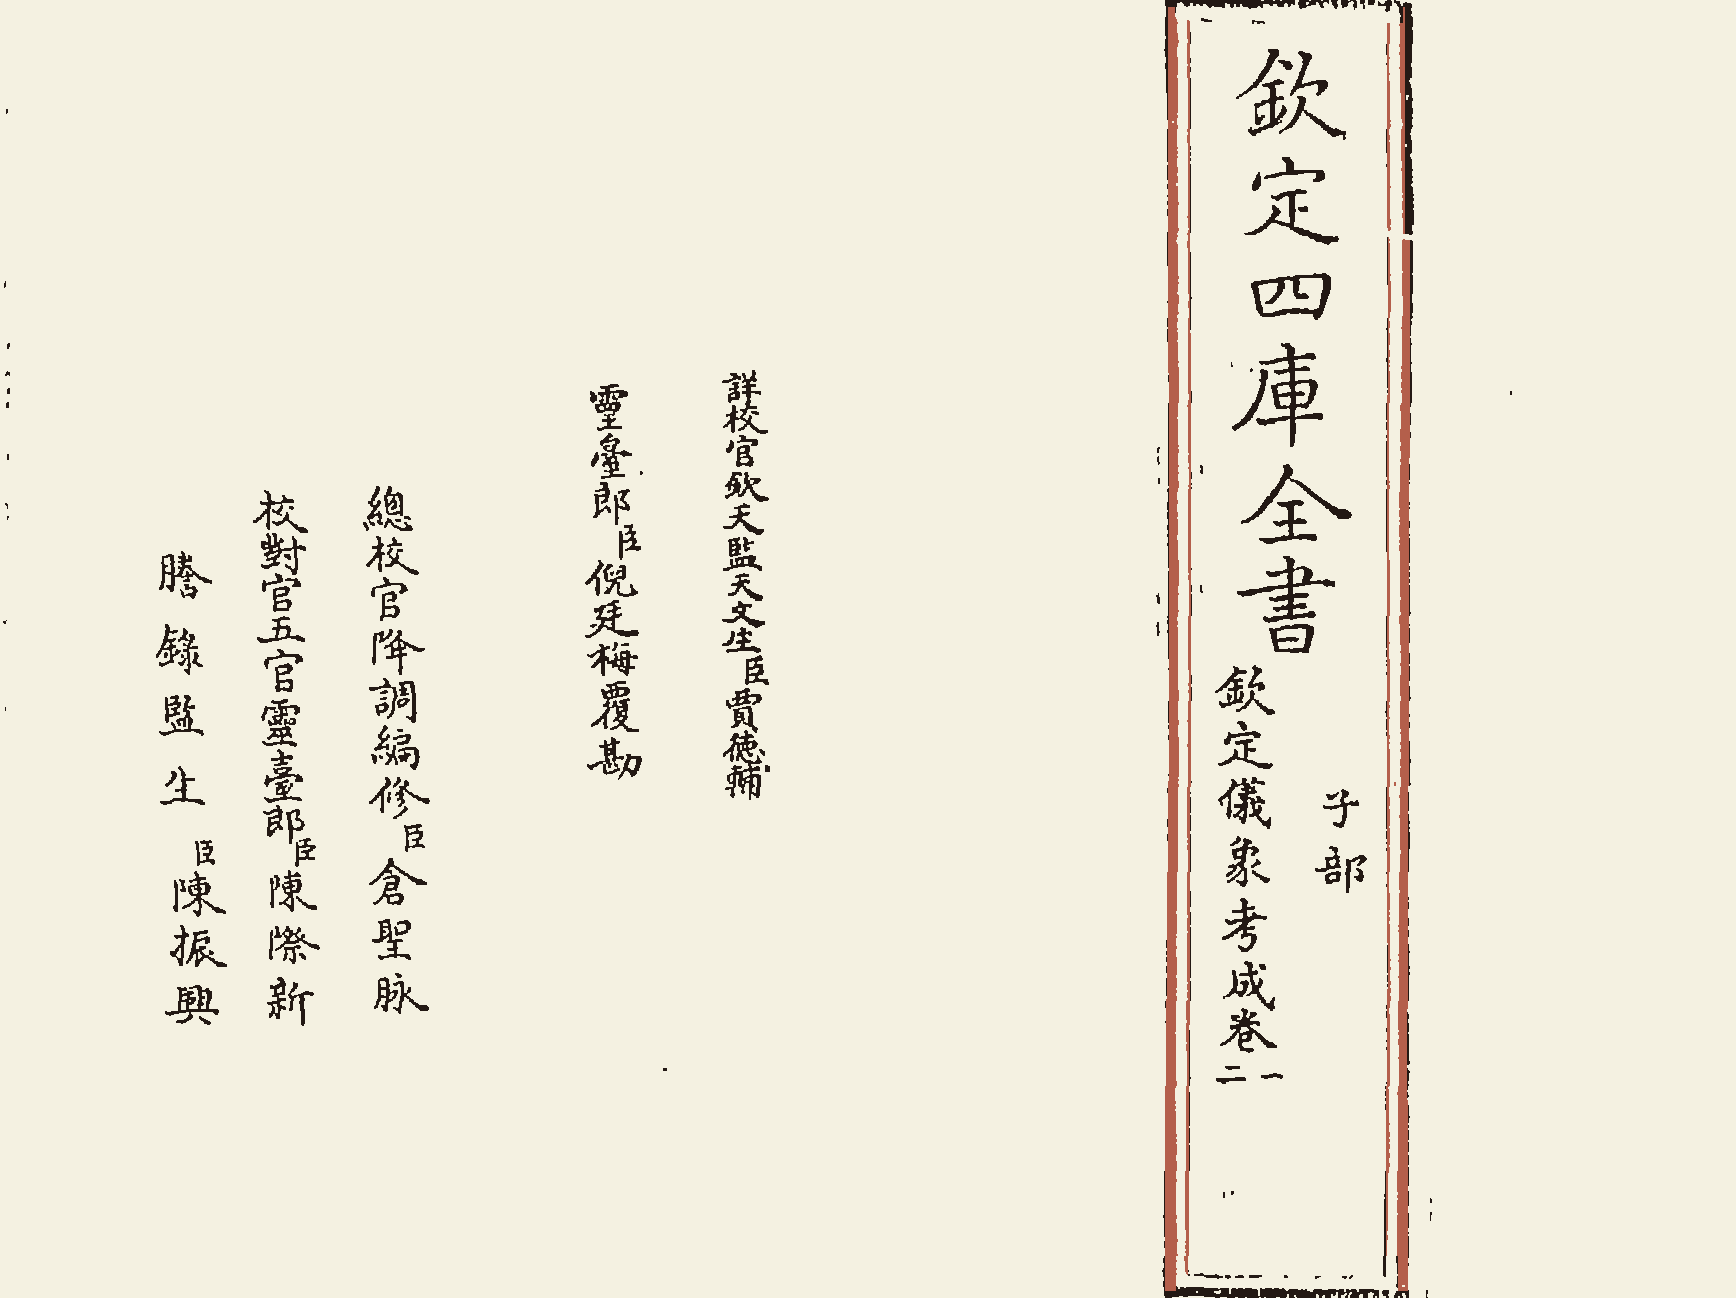
\includegraphics[width=\paperwidth,height=\paperheight,keepaspectratio]{img/0400.png}\clearpage
\begin{正文}
% ---- 册793 葉401 ----
\SetPageNumber{1}
欽定四庫全書\换行
欽定儀象考成卷一\换行
　恒星總紀\换行
　　三垣\换行
　　一十八宿\换行
　　恒星全圖\换行
　　赤道北恒星圖\换行
　　赤道南恒星圖\换行
\char"200B\relax\换行
\char"200B\relax\换行
\char"200B\relax\换行
\char"200B\relax\换行
\char"200B\relax\换行
\char"200B\relax\换行
\char"200B\relax\换行
\char"200B\relax
\par
% ---- 册793 葉404 ----
　　恒星總紀\换行
恒星即經星也以其有常不易故名經星\双列{\右小列{史記天官書}\左小列{紫宫房心權}}\换行
\双列{\右小列{衡咸池虚危列宿部星此天之五宫坐}\左小列{位也為經不移徙大小有差濶狹有常}}經星又各有經\换行
緯度故别之曰恒星其星官名數古今不同漢書天文\换行
志經星常宿中外官凡百一十八名積數七百八十三\换行
星晉志載呉太史令陳卓始列甘石巫咸三家星官著\换行
於圖録凡二百八十三官一千四百六十四星今皆不\换行
見原本隋丹元子歩天歌與陳卓數合後此言天官者\换行
皆以歩天歌為凖康熙十三年監臣南懐仁修儀象志\换行
星名與古同者總二百五十九座一千一百二十九星\换行
比歩天歌少二十四座三百三十五星又於有名常數\换行
之外増五百九十七星又多近南極星二十三座一百\换行
五十星近年以來累加測騐星官度數儀象志尚多未\换行
合又星之次第多不順序亦宜釐正於是逐星測量推\换行
其度數觀其形象序其次第著之於圖計三垣二十八\换行
宿星名與古同者總二百七十七座一千三百一十九
\par
% ---- 册793 葉405 ----
星比儀象志多十八座一百九十星與歩天歌為近其\换行
尤與古合者二十八宿次舍自古皆觜宿在前參宿在\换行
後其以何星作距古無明文唐書云古以參右肩為距\换行
失之太逺文獻通考載宋兩朝天文志云觜三星距西\换行
南星參十星距中星西第一星西法觜宿距中上星參\换行
宿亦距中西一星今按觜宿中上星在西南星前僅六\换行
分餘而西南星小中上星大則以中上星作距可也若\换行
參宿以中西一星作距星則觜宿之黄道度已在參宿\换行
後一度餘即赤道度亦在參宿後三十一分餘今依次\换行
順序以參宿中三星之東一星作距星則觜宿黄道度\换行
恒在參前一度弱與觜前參後之序合其餘諸座之星\换行
皆以次順序無凌躐顛倒之弊又於有名常數之外増\换行
一千六百一十四星近某座者即名某座増星依次分\换行
註方位以備稽考其近南極星二十三座一百五十星\换行
中國所不見仍依西測之舊共計恒星三百座三千八\换行
十三星編為總紀一卷庶星官名數古今不同及黄道
\par
% ---- 册793 葉408 ----
赤道所屬宫次皆展卷瞭然矣\换行
\char"200B\relax\换行
\char"200B\relax\换行
\char"200B\relax\换行
\char"200B\relax\换行
\char"200B\relax\换行
\char"200B\relax\换行
\char"200B\relax\换行
\char"200B\relax\换行
\char"200B\relax\换行
\char"200B\relax\换行
\char"200B\relax\换行
\char"200B\relax\换行
\char"200B\relax\换行
\char"200B\relax\换行
\char"200B\relax
\par
% ---- 册793 葉409 ----
紫微垣\换行
北極五星一太子二帝星三庶子四后宫五天樞外庶\换行
子増三星后宫増一星黄道在午未宫赤道在卯辰宫\换行
四輔四星外増一星黄道在未宫赤道在已午宫\换行
勾陳六星外増十星黄道在未申宫赤道在丑寅卯戌\换行
亥宫\换行
天皇大帝一星黄道在申宫赤道在亥宫\换行
天柱五星外増六星黄道在申酉宫赤道在子丑宫\换行
御女四星外増一星黄道在未申酉宫赤道在丑寅宫\换行
女史一星外増一星黄道在未宫赤道在寅宫\换行
柱史一星外増二星黄道在申宫赤道在丑宫\换行
尚書五星外増二星黄道在辰已午宫赤道在寅宫\换行
天床六星外増一星黄道在巳午宫赤道在寅卯宫\换行
大理二星外増一星黄道在未宫赤道在辰巳宫\换行
陰德二星外増一星黄道在未宫赤道在巳宫\换行
六甲六星外増一星黄道赤道俱在未申宫
\par
% ---- 册793 葉412 ----
五帝内座五星外増二星黄道在申宫赤道在酉戌宫\换行
華葢七星黄道在酉宫赤道在戌宫\换行
杠九星附華葢為一座外増一星黄道在申酉宫赤道\换行
在酉戌宫\换行
右垣墻七星一右樞二少尉三上輔四少輔五上衛六\换行
少衛七上丞外少尉増二星上輔増二星少輔増一星\换行
上衛増三星少衛増一星上丞増三星黄道在已午未\换行
申宫赤道在辰已午未申酉宫\换行
左垣墻八星一左樞二上宰三少宰四上弼五少弼六\换行
上衛七少衛八少丞外上衛増三星少衛増八星少丞\换行
増一星黄道在辰已酉宫赤道在戌亥子丑寅卯宫\换行
天乙一星黄道在已宫赤道在辰宫\换行
太乙一星黄道在午宫赤道在辰宫\换行
内厨二星外増二星黄道在午宫赤道在辰宫\换行
北斗七星一天樞二天璇三天璣四天權五玉衡六開\换行
陽七揺光外天樞増三星天璇増八星天權増三星開
\par
% ---- 册793 葉413 ----
陽増二星黄道在已午宫赤道在辰已宫\换行
輔一星附北斗為一座外増三星黄道在已宫赤道在\换行
辰宫\换行
天槍三星外増四星黄道在已宫赤道在卯宫\换行
元戈一星外増二星黄道在辰宫赤道在卯宫\换行
三公三星黄道在已宫赤道在辰宫\换行
相一星外増三星黄道在已宫赤道在辰宫\换行
天理四星外増一星黄道在午宫赤道在已宫\换行
太陽守一星外増一星黄道赤道俱在巳宫\换行
太尊一星黄道在午宫赤道在巳宫\换行
天牢六星外増二星黄道在巳午宫赤道在巳宫\换行
勢四星外増十六星黄道在午宫赤道在巳宫\换行
文昌六星外増八星黄道在午未宫赤道在午宫\换行
内階六星外増十星黄道在未宫赤道在午宫\换行
三師三星外増一星黄道在未宫赤道在午宫\换行
八榖八星外増三十四星黄道赤道俱在申宫
\par
% ---- 册793 葉416 ----
傳舍九星外増四星黄道在申酉宫赤道在酉戌亥宫\换行
天厨六星外増二星黄道在戌宫赤道在子丑宫\换行
天棓五星外増十星黄道赤道俱在寅宫\换行
　右共三十七座一百六十三星外増一百七十七星\换行
太微垣\换行
五帝座五星外増三星黄道赤道俱在巳宫\换行
太子一星黄道赤道俱在巳宫\换行
從官一星黄道赤道俱在巳宫\换行
幸臣一星黄道赤道俱在巳宫\换行
五諸侯五星外増七星黄道在辰巳宫赤道在辰宫\换行
九卿三星外増九星黄道赤道俱在辰宫\换行
三公三星黄道赤道俱在辰宫\换行
内屏四星外増六星黄道赤道俱在巳宫\换行
右垣墻五星一右執法二上將三次將四次相五上相\换行
外次相増三星上相増二星黄道赤道俱在巳宫\换行
左垣墻五星一左執法二上相三次相四次將五上將
\par
% ---- 册793 葉417 ----
外左執法增一星次相増一星次將増三星上將増二\换行
星黄道赤道俱在辰宫\换行
郎將一星外増二星黄道在巳宫赤道在辰宫\换行
郎位十五星外増三星黄道在巳宫赤道在辰巳宫\换行
常陳七星外増六星黄道在巳宫赤道在辰巳宫\换行
三台六星上台二星中台二星下台二星外上台増七\换行
星中台増三星下台増二星黄道在巳午未宫赤道在\换行
巳午宫\换行
虎賁一星黄道赤道俱在巳宫\换行
少微四星外增八星黄道在巳午宫赤道在巳宫\换行
長垣四星外増九星黄道在巳午宫赤道在巳宫\换行
靈臺三星外増八星黄道赤道俱在巳宫\换行
明堂三星外増六星黄道赤道俱在巳宫\换行
謁者一星外増二星黄道在巳宫赤道在辰宫\换行
　右共二十座七十八星外増九十三星\换行
天市垣
\par
% ---- 册793 葉420 ----
帝座一星黄道赤道俱在寅宫\换行
候一星外増五星黄道赤道俱在寅宫\换行
宦者四星外増五星黄道赤道俱在寅宫\换行
斗五星外増十四星黄道在寅卯宫赤道在寅宫\换行
斛四星外増三星黄道赤道俱在寅宫\换行
列肆二星外増四星黄道在寅卯宫赤道在寅宫\换行
車肆二星外増二星黄道赤道俱在寅宫\换行
市樓六星外増一星黄道赤道俱在寅宫\换行
宗正二星外増三星黄道赤道俱在寅宫\换行
宗人四星外増四星黄道赤道俱在寅宫\换行
宗二星黄道赤道俱在丑宫\换行
帛度二星外増三星黄道赤道俱在寅宫\换行
屠肆二星外増三星黄道赤道俱在丑寅宫\换行
右垣墻十一星一河中二河間三晉四鄭五周六秦七\换行
蜀八巴九梁十楚十一韓外河間増一星晉増三星周\换行
増十四星秦増一星蜀増二星巴増四星黄道赤道俱
\par
% ---- 册793 葉421 ----
在寅卯宫\换行
左垣墻十一星一魏二趙三九河四中山五齊六呉越\换行
七徐八東海九燕十南海十一宋外魏増八星趙増三\换行
星九河増一星中山増七星齊増八星呉越増七星徐\换行
増四星東海増四星宋増二星黄道赤道俱在丑寅宫\换行
天紀九星外増十四星黄道在寅卯宫赤道在寅宫\换行
女牀三星黄道赤道俱在寅宫\换行
貫索九星外増十三星黄道赤道俱在卯宫\换行
七公七星外増十六星黄道在卯辰宫赤道在寅卯宫\换行
　右共十九座八十七星外増一百五十九星\换行
角宿\换行
角宿二星外増十五星黄道赤道俱在辰宫\换行
平道二星黄道赤道俱在辰宫\换行
天田二星外増六星黄道赤道俱在辰宫\换行
周鼎三星黄道在辰巳宫赤道在辰宫\换行
進賢一星外増九星黄道赤道俱在辰宫
\par
% ---- 册793 葉424 ----
天門二星外増十一星黄道赤道俱在辰宫\换行
平二星外増三星黄道在卯辰宫赤道在辰宫\换行
庫樓十星外増一星黄道赤道俱在卯辰宫\换行
柱十一星黄道赤道俱在卯辰宫\换行
衡四星黄道在卯宫赤道在辰宫\换行
南門二星外増二星黄道在卯宫赤道在卯辰宫\换行
　右共十一座四十一星外増四十七星\换行
亢宿\换行
亢宿四星外増十二星黄道在卯宫赤道在卯辰宫\换行
大角一星外増一星黄道在辰宫赤道在卯宫\换行
右攝提三星外増三星黄道赤道俱在辰宫\换行
左攝提三星外増三星黄道在卯辰宫赤道在卯宫\换行
折威七星外増六星黄道赤道俱在卯宫\换行
頓頑二星外増一星黄道赤道俱在卯宫\换行
陽門二星黄道赤道俱在卯宫\换行
　右共七座二十二星外増二十六星
\par
% ---- 册793 葉425 ----
氐宿\换行
氐宿四星外増二十九星黄道赤道俱在卯宫\换行
亢池四星黄道在辰宫赤道在卯辰宫\换行
帝席三星外増一星黄道赤道俱在辰宫\换行
梗河三星外増五星黄道在卯辰宫赤道在卯宫\换行
招揺一星黄道在辰宫赤道在卯宫\换行
天乳一星外増三星黄道赤道俱在卯宫\换行
天輻二星外増一星黄道赤道俱在卯宫\换行
陣車三星外増二星黄道赤道俱在卯宫\换行
騎官十星黄道赤道俱在卯宫\换行
車騎三星黄道赤道俱在卯宫\换行
將軍一星黄道赤道俱在卯宫\换行
　右共十一座三十五星外増四十一星\换行
房宿\换行
房宿四星外増六星黄道赤道俱在卯宫\换行
鈎鈐二星附房宿為一座黄道在寅宫赤道在卯宫
\par
% ---- 册793 葉428 ----
鍵閉一星黄道在卯宫赤道在寅宫\换行
罰三星外増三星黄道在卯宫赤道在寅卯宫\换行
西咸四星外増二星黄道赤道俱在卯宫\换行
東咸四星外増一星黄道赤道俱在寅宫\换行
日一星外増一星黄道赤道俱在卯宫\换行
從官二星外増一星黄道赤道俱在卯宫\换行
　右共七座二十一星外増十四星\换行
心宿\换行
心宿三星外増八星黄道赤道俱在寅宫\换行
積卒二星黄道在寅宫赤道在卯宫\换行
　右共二座五星外増八星\换行
尾宿\换行
尾宿九星外増一星黄道赤道俱在寅宫\换行
神宫一星附尾宿為一座黄道赤道俱在寅宫\换行
天江四星外増十一星黄道赤道俱在寅宫\换行
傅説一星黄道赤道俱在寅宫
\par
% ---- 册793 葉429 ----
魚一星黄道赤道俱在寅宫\换行
龜五星黄道赤道俱在寅宫\换行
　右共五座二十一星外増十二星\换行
箕宿\换行
箕宿四星黄道赤道俱在丑寅宫\换行
糠一星黄道赤道俱在寅宫\换行
杵三星外増一星黄道赤道俱在寅宫\换行
　右共三座八星外増一星\换行
斗宿\换行
斗宿六星外増四星黄道赤道俱在丑寅宫\换行
天籥八星外増四星黄道赤道俱在寅宫\换行
天弁九星外増五星黄道赤道俱在丑宫\换行
建六星外増八星黄道赤道俱在丑宫\换行
天雞二星外増三星黄道赤道俱在丑宫\换行
狗二星外増六星黄道赤道俱在丑宫\换行
狗國四星黄道赤道俱在丑宫
\par
% ---- 册793 葉432 ----
天淵三星黄道赤道俱在丑宫\换行
農丈人一星黄道赤道俱在丑宫\换行
鼈十一星黄道赤道俱在丑宫\换行
　右共十座五十二星外増三十星\换行
牛宿\换行
牛宿六星外増九星黄道赤道俱在子丑宫\换行
天桴四星外増二星黄道在子丑宫赤道在丑宫\换行
河鼓三星外増九星黄道赤道俱在丑宫\换行
右旗九星外増十二星黄道赤道俱在丑宫\换行
左旗九星外増二十九星黄道赤道俱在子丑宫\换行
織女三星外増四星黄道赤道俱在丑宫\换行
漸臺四星外増六星黄道赤道俱在丑宫\换行
輦道五星外増九星黄道在子丑宫赤道在丑宫\换行
羅堰三星外增一星黄道赤道俱在子宫\换行
天田四星黄道赤道俱在子宫\换行
九坎四星黄道赤道俱在子宫
\par
% ---- 册793 葉433 ----
　右共十一座五十四星外増八十一星\换行
女宿\换行
女宿四星外増五星黄道赤道俱在子宫\换行
離珠四星外増一星黄道赤道俱在子宫\换行
敗𤓰五星外増三星黄道赤道俱在子宫\换行
瓠𤓰五星外増五星黄道赤道俱在子宫\换行
天津九星外増三十八星黄道在亥子宫赤道在子丑\换行
宫\换行
奚仲四星外増七星黄道在子宫赤道在丑宫\换行
扶筐七星外増四星黄道在子丑宫赤道在丑宫\换行
十二國十六星周二星秦二星代二星趙二星越一星\换行
齊一星楚一星鄭一星魏一星韓一星晉一星燕一星\换行
外代増二星黄道赤道俱在子宫\换行
　右共八座五十四星外増六十五星\换行
虚宿\换行
虚宿二星外増八星黄道赤道俱在子宫
\par
% ---- 册793 葉436 ----
司命二星黄道赤道俱在子宫\换行
司禄二星外増二星黄道赤道俱在子宫\换行
司危二星黄道赤道俱在子宫\换行
司非二星外増二星黄道赤道俱在子宫\换行
哭二星外増四星黄道赤道俱在子宫\换行
泣二星外増二星黄道在亥子宫赤道在亥宫\换行
離瑜三星外増三星黄道赤道俱在子宫\换行
天壘城十三星黄道赤道俱在子宫\换行
敗臼四星外増一星黄道在子宫赤道在亥子宫\换行
　右共十座三十四星外増二十二星\换行
危宿\换行
危宿三星外増十一星黄道在亥子宫赤道在子宫\换行
墳墓四星附危宿為一座外増四星黄道赤道俱在亥\换行
宫\换行
葢屋二星黄道赤道俱在子宫\换行
虚梁四星黄道赤道俱在亥宫
\par
% ---- 册793 葉437 ----
天錢五星外増四星黄道赤道俱在子宫\换行
人四星外増四星黄道在亥子宫赤道在子宫\换行
杵三星外増二星黄道在亥宫赤道在亥子宫\换行
臼四星外増五星黄道在亥宫赤道在亥子宫\换行
車府七星外増十九星黄道在戌亥宫赤道在亥子宫\换行
造父五星外増五星黄道在戌宫赤道在亥子宫\换行
天鉤九星外増十六星黄道在酉戌宫赤道在亥子宫\换行
　右共十座五十星外増七十星\换行
室宿\换行
室宿二星外増七星黄道赤道俱在亥宫\换行
離宫六星附室宿為一座外増八星黄道赤道俱在亥\换行
宫\换行
螣蛇二十二星外増十四星黄道在戌亥宫赤道在亥\换行
子宫\换行
雷電六星外増八星黄道赤道俱在亥宫\换行
土公吏二星黄道赤道俱在亥宫
\par
% ---- 册793 葉440 ----
壘壁陣十二星外増七星黄道赤道俱在亥子宫\换行
羽林軍四十五星黄道赤道俱在亥子宫\换行
天綱一星黄道在子宫赤道在亥宫\换行
北落師門一星黄道赤道俱在亥宫\换行
鈇鉞三星外増二星黄道赤道俱在亥宫\换行
八魁六星黄道在亥宫赤道在戌亥宫\换行
　右共十座一百零六星外増四十六星\换行
壁宿\换行
壁宿二星外増二十三星黄道在戌宫赤道在戌亥宫\换行
天廐三星外増一星黄道赤道俱在戌宫\换行
土公二星外増十一星黄道在戌宫赤道在戌亥宫\换行
霹𩆝五星外増八星黄道赤道俱在亥宫\换行
雲雨四星外増九星黄道赤道俱在亥宫\换行
鈇鑕五星黄道赤道俱在戌宫\换行
　右共六座二十一星外増五十二星\换行
奎宿
\par
% ---- 册793 葉441 ----
奎宿十六星外増二十二星黄道赤道俱在戌宫\换行
王良五星外増五星黄道在酉宫赤道在戌亥宫\换行
䇿一星黄道在酉宫赤道在戌宫\换行
附路一星黄道在酉宫赤道在戌宫\换行
軍南門一星黄道在酉宫赤道在戌宫\换行
閣道六星外増五星黄道赤道俱在酉戌宫\换行
外屏七星外増十五星黄道赤道俱在戌宫\换行
天溷四星外増六星黄道赤道俱在戌宫\换行
土司空一星黄道在亥宫赤道在戌宫\换行
　右共九座四十二星外増五十三星\换行
婁宿\换行
婁宿三星外増十五星黄道在酉戌宫赤道在戌宫\换行
天大將軍十一星外増十六星黄道在酉宫赤道在酉\换行
戌宫\换行
右更五星外増五星黄道赤道俱在戌宫\换行
左更五星外増七星黄道赤道俱在酉宫
\par
% ---- 册793 葉444 ----
天倉六星外増十八星黄道在戌亥宫赤道在戌宫\换行
天庾三星外増三星黄道在戌宫赤道在酉戌宫\换行
　右共六座三十三星外増六十四星\换行
胃宿\换行
胃宿三星外増五星黄道赤道俱在酉宫\换行
大陵八星外増二十星黄道赤道俱在酉宫\换行
積尸一星黄道赤道俱在酉宫\换行
天船九星外増九星黄道在申酉宫赤道在酉宫\换行
積水一星外増一星黄道在申宫赤道在酉宫\换行
天廩四星外増二星黄道赤道俱在酉宫\换行
天囷十三星外増二十星黄道赤道俱在酉戌宫\换行
　右共七座三十九星外増五十七星\换行
昴宿\换行
昴宿七星外増五星黄道赤道俱在酉宫\换行
天阿一星黄道赤道俱在酉宫\换行
月一星外増一星黄道赤道俱在酉宫
\par
% ---- 册793 葉445 ----
卷舌六星外増六星黄道在申酉宫赤道在酉宫\换行
天讒一星黄道赤道俱在酉宫\换行
礪石四星黄道在申宫赤道在申酉宫\换行
天陰五星外増四星黄道赤道俱在酉宫\换行
蒭藁六星外増五星黄道在戌宫赤道在酉宫\换行
天苑十六星外増十六星黄道在酉戌宫赤道在酉宫\换行
　右共九座四十七星外増三十七星\换行
畢宿\换行
畢宿八星外増十三星黄道赤道俱在申酉宫\换行
附耳一星附畢宿為一座外増一星黄道赤道俱在申\换行
宫\换行
天街二星外増四星黄道赤道俱在申宫\换行
天髙四星外増四星黄道赤道俱在申宫\换行
諸王六星外増四星黄道赤道俱在申宫\换行
五車五星外増十八星黄道赤道俱在申宫\换行
柱九星黄道赤道俱在申宫
\par
% ---- 册793 葉448 ----
咸池三星黄道赤道俱在申宫\换行
天潢五星外増二星黄道赤道俱在申宫\换行
天闗一星外増六星黄道赤道俱在申宫\换行
天節八星黄道赤道俱在申宫\换行
九州殊口六星外増十星黄道赤道俱在申酉宫\换行
參旗九星外増十一星黄道赤道俱在申宫\换行
九斿九星外増五星黄道赤道俱在申宫\换行
天園十三星外増六星黄道在酉戌亥宫赤道在申酉\换行
戌宫\换行
　右共十四座八十九星外増八十四星\换行
觜宿\换行
觜宿三星黄道赤道俱在申宫\换行
司怪四星外増六星黄道赤道俱在申宫\换行
座旗九星外増十一星黄道赤道俱在未宫\换行
　右共三座十六星外増十七星\换行
參宿
\par
% ---- 册793 葉449 ----
參宿七星外増三十七星黄道赤道俱在申宫\换行
伐三星附參宿為一座外増二星黄道赤道俱在申宫\换行
玉井四星外増二星黄道赤道俱在申宫\换行
軍井四星外増一星黄道赤道俱在申宫\换行
屏二星黄道赤道俱在申宫\换行
厠四星外増七星黄道赤道俱在申宫\换行
屎一星黄道赤道俱在申宫\换行
　右共六座二十五星外増四十九星\换行
井宿\换行
井宿八星外増十七星黄道赤道俱在未宫\换行
龯一星附井宿為一座外増一星黄道赤道俱在申宫\换行
水府四星外増八星黄道赤道俱在未申宫\换行
天罇三星外増九星黄道赤道俱在未宫\换行
五諸侯五星外増五星黄道赤道俱在未宫\换行
北河三星外増四星黄道赤道俱在未宫\换行
積水一星黄道赤道俱在未宫
\par
% ---- 册793 葉452 ----
積薪一星外増三星黄道赤道俱在未宫\换行
水位四星外増十一星黄道赤道俱在未宫\换行
南河三星外増十星黄道赤道俱在未宫\换行
四瀆四星外増六星黄道赤道俱在未宫\换行
闕邱二星外増七星黄道赤道俱在未宫\换行
軍市六星外増五星黄道赤道俱在未宫\换行
野雞一星黄道赤道俱在未宫\换行
天狼一星外増五星黄道赤道俱在未宫\换行
丈人二星黄道赤道俱在申宫\换行
子二星外増一星黄道赤道俱在申宫\换行
孫二星外増四星黄道赤道俱在未申宫\换行
老人一星外増四星黄道赤道俱在未宫\换行
弧矢九星外増二十四星黄道在午未宫赤道在未宫\换行
　右共十九座六十三星外増一百二十四星\换行
鬼宿\换行
鬼宿四星外増十八星黄道赤道俱在午宫
\par
% ---- 册793 葉453 ----
積尸氣一星外増三星黄道赤道俱在午宫\换行
爟四星外増十一星黄道赤道俱在未宫\换行
外厨六星外増十七星黄道赤道俱在午宫\换行
天記一星外増二星黄道在己宫赤道在午宫\换行
天狗七星黄道在巳午宫赤道在午宫\换行
天社六星外増五星黄道在辰巳午宫赤道在午宫\换行
　右共六座二十九星外増五十七星\换行
柳宿\换行
柳宿八星外増十星黄道赤道俱在午宫\换行
酒旗三星外増五星黄道赤道俱在午宫\换行
　右共二座十一星外増十五星\换行
星宿\换行
星宿七星外増十五星黄道赤道俱在午宫\换行
天相三星外増十二星黄道在己宫赤道在己午宫\换行
軒轅十七星外増五十七星黄道赤道俱在己午宫\换行
内平四星外増十一星黄道在午宫赤道在己午宫
\par
% ---- 册793 葉456 ----
　右共四座三十一星外増九十五星\换行
張宿\换行
張宿六星外増四星黄道赤道俱在己午宫\换行
　右一座六星外増四星\换行
翼宿\换行
翼宿二十二星外增七星黄道在辰己宫赤道在己宫\换行
　右一座二十二星外増七星\换行
軫宿\换行
軫宿四星外増五星黄道在辰宫赤道在辰己宫\换行
右轄一星附軫宿為一座黄道在辰宫赤道在己宫\换行
左轄一星附軫宿為一座黄道赤道俱在辰宫\换行
長沙一星附軫宿為一座黄道赤道俱在辰宫\换行
青邱七星外増三星黄道在辰宫赤道在己宫\换行
　右共二座十四星外増八星\换行
　總計三垣二十八宿共二百七十七座一千三百一\换行
　十九星外増一千六百一十四星按天文歩天歌角
\par
% ---- 册793 葉457 ----
　宿内柱十五星今少四星氐宿内亢池六星今少二\换行
　星騎官二十七星今少十七星心宿内積卒十二星\换行
　今少十星斗宿内天淵十星今少七星鼈十四星今\换行
　少三星牛宿内天田九星今少五星九坎九星今少\换行
　五星女宿内離珠五星今少一星危宿内天錢十星\换行
　今少五星人五星今少一星室宿内八魁九星今少\换行
　三星壁宿内天廐十星今少七星奎宿内天溷七星\换行
　今少三星畢宿内九州殊口九星今少三星井宿内\换行
　軍市十三星今少七星共少八十三星星宿内天稷\换行
　五星張宿内天廟十四星翼宿内東甌五星軫宿内\换行
　軍門二星土司空四星器府三十二星共六座六十\换行
　二星今無\换行
近南極星\换行
海山六星外増二星黄道在卯辰宫赤道在己宫\换行
十字四星黄道在卯宫赤道在辰宫\换行
馬尾三星黄道在辰宫赤道在辰己宫
\par
% ---- 册793 葉460 ----
馬腹三星黄道在卯宫赤道在辰宫\换行
蜜蜂四星黄道在卯宫赤道在辰宫\换行
三角形三星外増四星黄道在寅宫赤道在寅卯宫\换行
異雀九星黄道在寅宫赤道在寅卯辰宫\换行
孔雀十一星外増四星黄道在丑寅宫赤道在子丑寅\换行
宫\换行
波斯十一星黄道赤道俱在子丑宫\换行
蛇尾四星黄道在丑宫赤道在戌亥子宫\换行
蛇腹四星黄道在亥子宫赤道在酉戌宫\换行
蛇首二星黄道在亥宫赤道在酉戌宫\换行
鳥喙七星外増一星黄道在子宫赤道在戌亥宫\换行
鶴十二星外増二星黄道在子宫赤道在亥子宫\换行
火鳥十星外増一星黄道在亥子宫赤道在戌亥宫\换行
水委三星黄道在亥宫赤道在戌宫\换行
附白二星黄道在子宫赤道在酉宫\换行
夾白二星黄道在戌亥宫赤道在申酉宫
\par
% ---- 册793 葉461 ----
金魚五星外増一星黄道在寅酉戌宫赤道在未申宫\换行
海石五星外増三星黄道在辰己宫赤道在午宫\换行
飛魚六星黄道在卯辰宫赤道在午未宫\换行
南船五星外増一星黄道在卯辰宫赤道在己午宫\换行
小斗九星外増一星黄道在寅卯宫赤道在辰巳午未\换行
宫\换行
　右共二十三座一百三十星外増二十星古無\换行
\char"200B\relax\换行
\char"200B\relax\换行
\char"200B\relax\换行
\char"200B\relax\换行
\char"200B\relax\换行
\char"200B\relax\换行
\char"200B\relax\换行
\char"200B\relax\换行
\char"200B\relax
\par
% ---- 册793 葉464 ----
　　恒星全圖\换行
唐書天文志葢天之説一行削篾為度徑一分其厚半\换行
之長與圖等穴其正中植鍼為樞令可環運自中樞之\换行
外均刻百四十七度全度之末旋為外規規外大半度\换行
再旋為重規以均賦周天度分又距極樞九十一度少\换行
半旋為赤道𢃄天之紘距極三十五度旋為内規乃歩\换行
冬至日躔所在以正辰次之中以立宿距按渾儀所測\换行
甘石巫咸衆星明者皆以篾横考入宿距縱考去極度\换行
而後圖之其赤道外衆星踈宻之狀與仰視小殊者由\换行
渾儀去南極漸近其度益狹而葢圖漸逺其度益廣使\换行
然若考其去極入宿度數移之於渾天則一也又赤道\换行
内外其廣狹不均若就二至出入赤道二十四度以規\换行
度之則二分所交不得其正自二分黄赤道交以規度\换行
之則二至距極度數不得其正當求黄赤分至之中均\换行
刻為七十二限據每黄道差數以篾度量而識之然後\换行
規為黄道則周天咸得其正矣今按渾天係圓體圖之
\par
% ---- 册793 葉465 ----
於平面止見其半故渾天不可圖葢天圖以北極為中\换行
心乃見星座全象然其内外二規亦猶是渾天之法也\换行
渾天家以北極出地常見不隠謂之上規南極入地常\换行
隠不見謂之下規一行葢天圖以三十五度為内規即\换行
上規之度也\双列{\右小列{北極出地}\左小列{三十五度}}一百四十七度為外規即北極\换行
距下規之度也\双列{\右小列{古法周天三百六十五度四分度之一}\左小列{則北極距南極為一百八十二度有竒}}\换行
\双列{\右小列{除南極入地三十五度}\左小列{有竒餘一百四十七度}}今法周天三百六十度赤道距\换行
南北極各九十度京師北極出地四十度故以四十度\换行
為内規中國幅隕南至北極出地二十度則北極距下\换行
規一百六十度故以一百六十度為外規其餘悉如一\换行
行之法依新測恒星赤道經緯度著之於圖仍用赤黄\换行
黒三色以存三家之舊又以赤道南北分為二圖則北\换行
極出地二十度以南所見之星座無不備具雖中天所\换行
見星座横分為二然赤道以南其度漸狹可以補葢天\换行
星度益廣之失合觀三圖則懸象著明躔離攸次星之\换行
隠見天漢昭回庶幾無遺憾矣
\par
\end{正文}\clearpage
\嵌图{141.61pt}{202.05pt}{848.55pt}{585.69pt}{img/0470.png}
\begin{正文}
% ---- 册793 葉470 图版 ----
\SetPageNumber{34}
\插图页
\char"200B\relax\换行
\char"200B\relax\换行
\char"200B\relax\换行
\char"200B\relax\换行
\char"200B\relax\换行
\char"200B\relax\换行
\char"200B\relax\换行
\char"200B\relax\换行
\char"200B\relax\换行
\char"200B\relax\换行
\char"200B\relax\换行
\char"200B\relax\换行
\char"200B\relax\换行
\char"200B\relax\换行
\char"200B\relax\换行
\char"200B\relax
\恢复丝栏\par
\end{正文}\clearpage
\嵌图{145.79pt}{200.67pt}{840.19pt}{588.45pt}{img/0474.png}
\begin{正文}
% ---- 册793 葉474 图版 ----
\SetPageNumber{35}
\插图页
\char"200B\relax\换行
\char"200B\relax\换行
\char"200B\relax\换行
\char"200B\relax\换行
\char"200B\relax\换行
\char"200B\relax\换行
\char"200B\relax\换行
\char"200B\relax\换行
\char"200B\relax\换行
\char"200B\relax\换行
\char"200B\relax\换行
\char"200B\relax\换行
\char"200B\relax\换行
\char"200B\relax\换行
\char"200B\relax\换行
\char"200B\relax
\恢复丝栏\par
\end{正文}\clearpage
\嵌图{147.13pt}{204.95pt}{837.49pt}{579.89pt}{img/0478.png}
\begin{正文}
% ---- 册793 葉478 图版 ----
\SetPageNumber{36}
\插图页
\char"200B\relax\换行
\char"200B\relax\换行
\char"200B\relax\换行
\char"200B\relax\换行
\char"200B\relax\换行
\char"200B\relax\换行
\char"200B\relax\换行
\char"200B\relax\换行
\char"200B\relax\换行
\char"200B\relax\换行
\char"200B\relax\换行
\char"200B\relax\换行
\char"200B\relax\换行
\char"200B\relax\换行
\char"200B\relax\换行
\char"200B\relax
\恢复丝栏\par

% ======== 卷二（8行21字）========
\par\end{正文}\clearpage
\chapter*{欽定儀象考成卷二}
\begin{正文}
% ---- 册793 葉480 ----
\SetPageNumber{1}
欽定四庫全書\换行
欽定儀象考成卷二\换行
　恒星黄道經緯度表一\换行
　　黄道星紀宫\双列{\右小列{赤道度附}\左小列{}}\换行
\char"200B\relax\换行
\char"200B\relax\换行
\char"200B\relax\换行
\char"200B\relax\换行
\char"200B\relax\换行
\char"200B\relax\换行
\char"200B\relax\换行
\char"200B\relax\换行
\char"200B\relax\换行
\char"200B\relax\换行
\char"200B\relax\换行
\char"200B\relax
\par
% ---- 册793 葉481 ----
　　恒星黄赤經緯度表\换行
恒星布列周天古有去極入宿度數入宿即經度也去\换行
極即緯度也然黄道度與赤道度不同嵗差亦異葢黄\换行
道以黄極為樞赤道以赤極為樞兩道兩極各相距二\换行
十三度半故星在兩極之間者黄道屬未宫赤道則屬\换行
丑宫星在兩道之間者黄道屬緯南赤道則屬緯北此\换行
黄赤不同之極致也恒星循黄道東行每年五十一秒\换行
緯度終古不改而經度之差有常赤道與黄道斜交分\换行
至前後南北逺近其差不等兩極之間在黄道為差而\换行
東在赤道為差而西兩交之際黄道南者差而入赤道\换行
北黄道北者差而出赤道南此嵗差不同之極致也今\换行
以乾隆九年甲子恒星黄赤經緯度依黄道次序列恒\换行
星黄道經緯度表而以赤道經緯附之依赤道次序列\换行
恒星赤道經緯度表而以黄道經緯附之各將赤道嵗\换行
差列於其下黄道以便推算赤道以便測量厯象之用\换行
於斯備矣
\par
\end{正文}\clearpage
\嵌图{142.64pt}{198.13pt}{846.47pt}{593.52pt}{img/0484.png}
\begin{正文}
% ---- 册793 葉484 图版 ----
\SetPageNumber{3}
\插图页
\char"200B\relax\换行
\char"200B\relax\换行
\char"200B\relax\换行
\char"200B\relax\换行
\char"200B\relax\换行
\char"200B\relax\换行
\char"200B\relax\换行
\char"200B\relax\换行
\char"200B\relax\换行
\char"200B\relax\换行
\char"200B\relax\换行
\char"200B\relax\换行
\char"200B\relax\换行
\char"200B\relax\换行
\char"200B\relax\换行
\char"200B\relax
\恢复丝栏\par
\end{正文}\clearpage
\嵌图{142.64pt}{198.61pt}{846.47pt}{592.57pt}{img/0485.png}
\begin{正文}
% ---- 册793 葉485 图版 ----
\SetPageNumber{4}
\插图页
\char"200B\relax\换行
\char"200B\relax\换行
\char"200B\relax\换行
\char"200B\relax\换行
\char"200B\relax\换行
\char"200B\relax\换行
\char"200B\relax\换行
\char"200B\relax\换行
\char"200B\relax\换行
\char"200B\relax\换行
\char"200B\relax\换行
\char"200B\relax\换行
\char"200B\relax\换行
\char"200B\relax\换行
\char"200B\relax\换行
\char"200B\relax
\恢复丝栏\par
\end{正文}\clearpage
\嵌图{144.63pt}{200.02pt}{842.50pt}{589.74pt}{img/0488.png}
\begin{正文}
% ---- 册793 葉488 图版 ----
\SetPageNumber{5}
\插图页
\char"200B\relax\换行
\char"200B\relax\换行
\char"200B\relax\换行
\char"200B\relax\换行
\char"200B\relax\换行
\char"200B\relax\换行
\char"200B\relax\换行
\char"200B\relax\换行
\char"200B\relax\换行
\char"200B\relax\换行
\char"200B\relax\换行
\char"200B\relax\换行
\char"200B\relax\换行
\char"200B\relax\换行
\char"200B\relax\换行
\char"200B\relax
\恢复丝栏\par
\end{正文}\clearpage
\嵌图{144.63pt}{200.00pt}{842.50pt}{589.78pt}{img/0489.png}
\begin{正文}
% ---- 册793 葉489 图版 ----
\SetPageNumber{6}
\插图页
\char"200B\relax\换行
\char"200B\relax\换行
\char"200B\relax\换行
\char"200B\relax\换行
\char"200B\relax\换行
\char"200B\relax\换行
\char"200B\relax\换行
\char"200B\relax\换行
\char"200B\relax\换行
\char"200B\relax\换行
\char"200B\relax\换行
\char"200B\relax\换行
\char"200B\relax\换行
\char"200B\relax\换行
\char"200B\relax\换行
\char"200B\relax
\恢复丝栏\par
\end{正文}\clearpage
\嵌图{148.54pt}{198.57pt}{834.68pt}{592.64pt}{img/0492.png}
\begin{正文}
% ---- 册793 葉492 图版 ----
\SetPageNumber{7}
\插图页
\char"200B\relax\换行
\char"200B\relax\换行
\char"200B\relax\换行
\char"200B\relax\换行
\char"200B\relax\换行
\char"200B\relax\换行
\char"200B\relax\换行
\char"200B\relax\换行
\char"200B\relax\换行
\char"200B\relax\换行
\char"200B\relax\换行
\char"200B\relax\换行
\char"200B\relax\换行
\char"200B\relax\换行
\char"200B\relax\换行
\char"200B\relax
\恢复丝栏\par
\end{正文}\clearpage
\嵌图{148.54pt}{197.60pt}{834.68pt}{594.58pt}{img/0493.png}
\begin{正文}
% ---- 册793 葉493 图版 ----
\SetPageNumber{8}
\插图页
\char"200B\relax\换行
\char"200B\relax\换行
\char"200B\relax\换行
\char"200B\relax\换行
\char"200B\relax\换行
\char"200B\relax\换行
\char"200B\relax\换行
\char"200B\relax\换行
\char"200B\relax\换行
\char"200B\relax\换行
\char"200B\relax\换行
\char"200B\relax\换行
\char"200B\relax\换行
\char"200B\relax\换行
\char"200B\relax\换行
\char"200B\relax
\恢复丝栏\par
\end{正文}\clearpage
\嵌图{148.61pt}{200.04pt}{834.55pt}{589.71pt}{img/0496.png}
\begin{正文}
% ---- 册793 葉496 图版 ----
\SetPageNumber{9}
\插图页
\char"200B\relax\换行
\char"200B\relax\换行
\char"200B\relax\换行
\char"200B\relax\换行
\char"200B\relax\换行
\char"200B\relax\换行
\char"200B\relax\换行
\char"200B\relax\换行
\char"200B\relax\换行
\char"200B\relax\换行
\char"200B\relax\换行
\char"200B\relax\换行
\char"200B\relax\换行
\char"200B\relax\换行
\char"200B\relax\换行
\char"200B\relax
\恢复丝栏\par
\end{正文}\clearpage
\嵌图{146.62pt}{199.56pt}{838.53pt}{590.67pt}{img/0497.png}
\begin{正文}
% ---- 册793 葉497 图版 ----
\SetPageNumber{10}
\插图页
\char"200B\relax\换行
\char"200B\relax\换行
\char"200B\relax\换行
\char"200B\relax\换行
\char"200B\relax\换行
\char"200B\relax\换行
\char"200B\relax\换行
\char"200B\relax\换行
\char"200B\relax\换行
\char"200B\relax\换行
\char"200B\relax\换行
\char"200B\relax\换行
\char"200B\relax\换行
\char"200B\relax\换行
\char"200B\relax\换行
\char"200B\relax
\恢复丝栏\par
\end{正文}\clearpage
\嵌图{142.64pt}{197.65pt}{846.47pt}{594.50pt}{img/0500.png}
\begin{正文}
% ---- 册793 葉500 图版 ----
\SetPageNumber{11}
\插图页
\char"200B\relax\换行
\char"200B\relax\换行
\char"200B\relax\换行
\char"200B\relax\换行
\char"200B\relax\换行
\char"200B\relax\换行
\char"200B\relax\换行
\char"200B\relax\换行
\char"200B\relax\换行
\char"200B\relax\换行
\char"200B\relax\换行
\char"200B\relax\换行
\char"200B\relax\换行
\char"200B\relax\换行
\char"200B\relax\换行
\char"200B\relax
\恢复丝栏\par
\end{正文}\clearpage
\嵌图{144.63pt}{199.49pt}{842.50pt}{590.81pt}{img/0501.png}
\begin{正文}
% ---- 册793 葉501 图版 ----
\SetPageNumber{12}
\插图页
\char"200B\relax\换行
\char"200B\relax\换行
\char"200B\relax\换行
\char"200B\relax\换行
\char"200B\relax\换行
\char"200B\relax\换行
\char"200B\relax\换行
\char"200B\relax\换行
\char"200B\relax\换行
\char"200B\relax\换行
\char"200B\relax\换行
\char"200B\relax\换行
\char"200B\relax\换行
\char"200B\relax\换行
\char"200B\relax\换行
\char"200B\relax
\恢复丝栏\par
\end{正文}\clearpage
\嵌图{144.68pt}{202.35pt}{842.41pt}{585.10pt}{img/0504.png}
\begin{正文}
% ---- 册793 葉504 图版 ----
\SetPageNumber{13}
\插图页
\char"200B\relax\换行
\char"200B\relax\换行
\char"200B\relax\换行
\char"200B\relax\换行
\char"200B\relax\换行
\char"200B\relax\换行
\char"200B\relax\换行
\char"200B\relax\换行
\char"200B\relax\换行
\char"200B\relax\换行
\char"200B\relax\换行
\char"200B\relax\换行
\char"200B\relax\换行
\char"200B\relax\换行
\char"200B\relax\换行
\char"200B\relax
\恢复丝栏\par
\end{正文}\clearpage
\嵌图{146.67pt}{202.84pt}{838.42pt}{584.11pt}{img/0505.png}
\begin{正文}
% ---- 册793 葉505 图版 ----
\SetPageNumber{14}
\插图页
\char"200B\relax\换行
\char"200B\relax\换行
\char"200B\relax\换行
\char"200B\relax\换行
\char"200B\relax\换行
\char"200B\relax\换行
\char"200B\relax\换行
\char"200B\relax\换行
\char"200B\relax\换行
\char"200B\relax\换行
\char"200B\relax\换行
\char"200B\relax\换行
\char"200B\relax\换行
\char"200B\relax\换行
\char"200B\relax\换行
\char"200B\relax
\恢复丝栏\par
\end{正文}\clearpage
\嵌图{144.72pt}{201.88pt}{842.31pt}{586.04pt}{img/0508.png}
\begin{正文}
% ---- 册793 葉508 图版 ----
\SetPageNumber{15}
\插图页
\char"200B\relax\换行
\char"200B\relax\换行
\char"200B\relax\换行
\char"200B\relax\换行
\char"200B\relax\换行
\char"200B\relax\换行
\char"200B\relax\换行
\char"200B\relax\换行
\char"200B\relax\换行
\char"200B\relax\换行
\char"200B\relax\换行
\char"200B\relax\换行
\char"200B\relax\换行
\char"200B\relax\换行
\char"200B\relax\换行
\char"200B\relax
\恢复丝栏\par
\end{正文}\clearpage
\嵌图{148.73pt}{202.36pt}{834.29pt}{585.07pt}{img/0509.png}
\begin{正文}
% ---- 册793 葉509 图版 ----
\SetPageNumber{16}
\插图页
\char"200B\relax\换行
\char"200B\relax\换行
\char"200B\relax\换行
\char"200B\relax\换行
\char"200B\relax\换行
\char"200B\relax\换行
\char"200B\relax\换行
\char"200B\relax\换行
\char"200B\relax\换行
\char"200B\relax\换行
\char"200B\relax\换行
\char"200B\relax\换行
\char"200B\relax\换行
\char"200B\relax\换行
\char"200B\relax\换行
\char"200B\relax
\恢复丝栏\par
\end{正文}\clearpage
\嵌图{144.63pt}{199.98pt}{842.50pt}{589.82pt}{img/0512.png}
\begin{正文}
% ---- 册793 葉512 图版 ----
\SetPageNumber{17}
\插图页
\char"200B\relax\换行
\char"200B\relax\换行
\char"200B\relax\换行
\char"200B\relax\换行
\char"200B\relax\换行
\char"200B\relax\换行
\char"200B\relax\换行
\char"200B\relax\换行
\char"200B\relax\换行
\char"200B\relax\换行
\char"200B\relax\换行
\char"200B\relax\换行
\char"200B\relax\换行
\char"200B\relax\换行
\char"200B\relax\换行
\char"200B\relax
\恢复丝栏\par
\end{正文}\clearpage
\嵌图{146.62pt}{201.36pt}{838.53pt}{587.07pt}{img/0513.png}
\begin{正文}
% ---- 册793 葉513 图版 ----
\SetPageNumber{18}
\插图页
\char"200B\relax\换行
\char"200B\relax\换行
\char"200B\relax\换行
\char"200B\relax\换行
\char"200B\relax\换行
\char"200B\relax\换行
\char"200B\relax\换行
\char"200B\relax\换行
\char"200B\relax\换行
\char"200B\relax\换行
\char"200B\relax\换行
\char"200B\relax\换行
\char"200B\relax\换行
\char"200B\relax\换行
\char"200B\relax\换行
\char"200B\relax
\恢复丝栏\par
\end{正文}\clearpage
\嵌图{167.87pt}{238.87pt}{125.06pt}{582.34pt}{img/0516.png}
\begin{正文}
% ---- 册793 葉516 ----
\SetPageNumber{19}
\char"200B\relax\换行
\char"200B\relax\换行
\char"200B\relax\换行
\char"200B\relax\换行
\char"200B\relax\换行
\char"200B\relax\换行
\char"200B\relax\换行
\char"200B\relax\换行
\char"200B\relax\换行
\char"200B\relax\换行
\char"200B\relax\换行
\char"200B\relax\换行
\char"200B\relax\换行
\char"200B\relax\换行
\char"200B\relax\换行
欽定儀象考成卷二
\par

\par\end{正文}\clearpage

  % ======== 卷三（8行21字）========
\chapter*{欽定儀象考成卷三}
\begin{正文}
\end{正文}\clearpage
\thispagestyle{empty}\noindent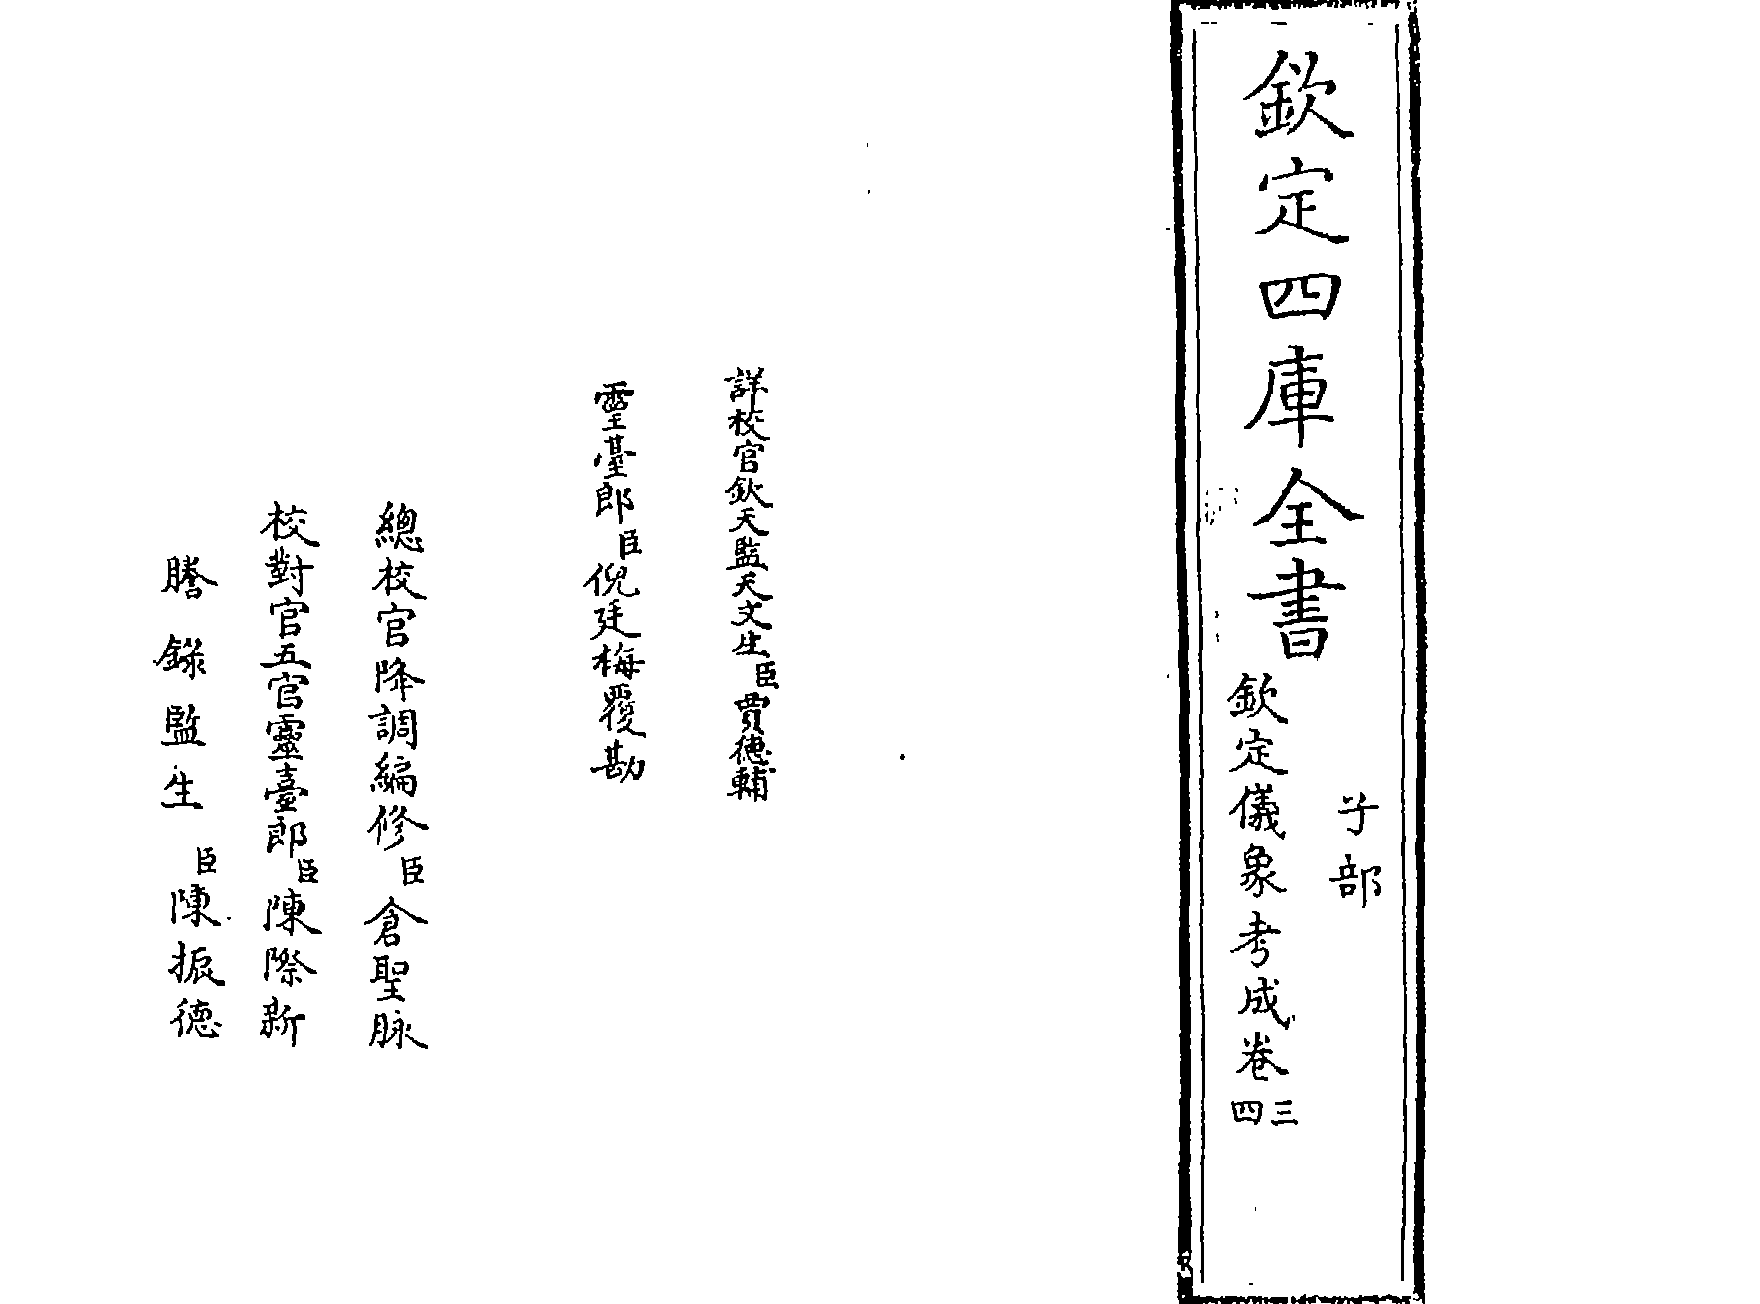
\includegraphics[width=\paperwidth,height=\paperheight,keepaspectratio]{img/0520.png}\clearpage
\begin{正文}
% ---- 册793 葉521 ----
\SetPageNumber{1}
欽定四庫全書\换行
欽定儀象考成卷三\换行
　恒星黄道經緯度表二\换行
　　黄道元枵宫\双列{\右小列{赤道度附}\左小列{}}\换行
\char"200B\relax\换行
\char"200B\relax\换行
\char"200B\relax\换行
\char"200B\relax\换行
\char"200B\relax\换行
\char"200B\relax\换行
\char"200B\relax\换行
\char"200B\relax\换行
\char"200B\relax\换行
\char"200B\relax\换行
\char"200B\relax\换行
\char"200B\relax
\par
\end{正文}\clearpage
\嵌图{142.64pt}{198.62pt}{846.47pt}{592.55pt}{img/0524.png}
\begin{正文}
% ---- 册793 葉524 图版 ----
\SetPageNumber{2}
\插图页
\char"200B\relax\换行
\char"200B\relax\换行
\char"200B\relax\换行
\char"200B\relax\换行
\char"200B\relax\换行
\char"200B\relax\换行
\char"200B\relax\换行
\char"200B\relax\换行
\char"200B\relax\换行
\char"200B\relax\换行
\char"200B\relax\换行
\char"200B\relax\换行
\char"200B\relax\换行
\char"200B\relax\换行
\char"200B\relax\换行
\char"200B\relax
\恢复丝栏\par
\end{正文}\clearpage
\嵌图{144.63pt}{197.19pt}{842.50pt}{595.40pt}{img/0525.png}
\begin{正文}
% ---- 册793 葉525 图版 ----
\SetPageNumber{3}
\插图页
\char"200B\relax\换行
\char"200B\relax\换行
\char"200B\relax\换行
\char"200B\relax\换行
\char"200B\relax\换行
\char"200B\relax\换行
\char"200B\relax\换行
\char"200B\relax\换行
\char"200B\relax\换行
\char"200B\relax\换行
\char"200B\relax\换行
\char"200B\relax\换行
\char"200B\relax\换行
\char"200B\relax\换行
\char"200B\relax\换行
\char"200B\relax
\恢复丝栏\par
\end{正文}\clearpage
\嵌图{142.68pt}{200.11pt}{846.40pt}{589.58pt}{img/0528.png}
\begin{正文}
% ---- 册793 葉528 图版 ----
\SetPageNumber{4}
\插图页
\char"200B\relax\换行
\char"200B\relax\换行
\char"200B\relax\换行
\char"200B\relax\换行
\char"200B\relax\换行
\char"200B\relax\换行
\char"200B\relax\换行
\char"200B\relax\换行
\char"200B\relax\换行
\char"200B\relax\换行
\char"200B\relax\换行
\char"200B\relax\换行
\char"200B\relax\换行
\char"200B\relax\换行
\char"200B\relax\换行
\char"200B\relax
\恢复丝栏\par
\end{正文}\clearpage
\嵌图{144.68pt}{202.93pt}{842.41pt}{583.94pt}{img/0529.png}
\begin{正文}
% ---- 册793 葉529 图版 ----
\SetPageNumber{5}
\插图页
\char"200B\relax\换行
\char"200B\relax\换行
\char"200B\relax\换行
\char"200B\relax\换行
\char"200B\relax\换行
\char"200B\relax\换行
\char"200B\relax\换行
\char"200B\relax\换行
\char"200B\relax\换行
\char"200B\relax\换行
\char"200B\relax\换行
\char"200B\relax\换行
\char"200B\relax\换行
\char"200B\relax\换行
\char"200B\relax\换行
\char"200B\relax
\恢复丝栏\par
\end{正文}\clearpage
\嵌图{144.63pt}{202.38pt}{842.50pt}{585.03pt}{img/0532.png}
\begin{正文}
% ---- 册793 葉532 图版 ----
\SetPageNumber{6}
\插图页
\char"200B\relax\换行
\char"200B\relax\换行
\char"200B\relax\换行
\char"200B\relax\换行
\char"200B\relax\换行
\char"200B\relax\换行
\char"200B\relax\换行
\char"200B\relax\换行
\char"200B\relax\换行
\char"200B\relax\换行
\char"200B\relax\换行
\char"200B\relax\换行
\char"200B\relax\换行
\char"200B\relax\换行
\char"200B\relax\换行
\char"200B\relax
\恢复丝栏\par
\end{正文}\clearpage
\嵌图{144.63pt}{201.44pt}{842.50pt}{586.92pt}{img/0533.png}
\begin{正文}
% ---- 册793 葉533 图版 ----
\SetPageNumber{7}
\插图页
\char"200B\relax\换行
\char"200B\relax\换行
\char"200B\relax\换行
\char"200B\relax\换行
\char"200B\relax\换行
\char"200B\relax\换行
\char"200B\relax\换行
\char"200B\relax\换行
\char"200B\relax\换行
\char"200B\relax\换行
\char"200B\relax\换行
\char"200B\relax\换行
\char"200B\relax\换行
\char"200B\relax\换行
\char"200B\relax\换行
\char"200B\relax
\恢复丝栏\par
\end{正文}\clearpage
\嵌图{142.68pt}{199.14pt}{846.40pt}{591.50pt}{img/0536.png}
\begin{正文}
% ---- 册793 葉536 图版 ----
\SetPageNumber{8}
\插图页
\char"200B\relax\换行
\char"200B\relax\换行
\char"200B\relax\换行
\char"200B\relax\换行
\char"200B\relax\换行
\char"200B\relax\换行
\char"200B\relax\换行
\char"200B\relax\换行
\char"200B\relax\换行
\char"200B\relax\换行
\char"200B\relax\换行
\char"200B\relax\换行
\char"200B\relax\换行
\char"200B\relax\换行
\char"200B\relax\换行
\char"200B\relax
\恢复丝栏\par
\end{正文}\clearpage
\嵌图{148.67pt}{201.53pt}{834.42pt}{586.72pt}{img/0537.png}
\begin{正文}
% ---- 册793 葉537 图版 ----
\SetPageNumber{9}
\插图页
\char"200B\relax\换行
\char"200B\relax\换行
\char"200B\relax\换行
\char"200B\relax\换行
\char"200B\relax\换行
\char"200B\relax\换行
\char"200B\relax\换行
\char"200B\relax\换行
\char"200B\relax\换行
\char"200B\relax\换行
\char"200B\relax\换行
\char"200B\relax\换行
\char"200B\relax\换行
\char"200B\relax\换行
\char"200B\relax\换行
\char"200B\relax
\恢复丝栏\par
\end{正文}\clearpage
\嵌图{144.68pt}{202.35pt}{842.41pt}{585.08pt}{img/0540.png}
\begin{正文}
% ---- 册793 葉540 图版 ----
\SetPageNumber{10}
\插图页
\char"200B\relax\换行
\char"200B\relax\换行
\char"200B\relax\换行
\char"200B\relax\换行
\char"200B\relax\换行
\char"200B\relax\换行
\char"200B\relax\换行
\char"200B\relax\换行
\char"200B\relax\换行
\char"200B\relax\换行
\char"200B\relax\换行
\char"200B\relax\换行
\char"200B\relax\换行
\char"200B\relax\换行
\char"200B\relax\换行
\char"200B\relax
\恢复丝栏\par
\end{正文}\clearpage
\嵌图{144.68pt}{201.91pt}{842.41pt}{585.98pt}{img/0541.png}
\begin{正文}
% ---- 册793 葉541 图版 ----
\SetPageNumber{11}
\插图页
\char"200B\relax\换行
\char"200B\relax\换行
\char"200B\relax\换行
\char"200B\relax\换行
\char"200B\relax\换行
\char"200B\relax\换行
\char"200B\relax\换行
\char"200B\relax\换行
\char"200B\relax\换行
\char"200B\relax\换行
\char"200B\relax\换行
\char"200B\relax\换行
\char"200B\relax\换行
\char"200B\relax\换行
\char"200B\relax\换行
\char"200B\relax
\恢复丝栏\par
\end{正文}\clearpage
\嵌图{144.63pt}{200.50pt}{842.50pt}{588.79pt}{img/0544.png}
\begin{正文}
% ---- 册793 葉544 图版 ----
\SetPageNumber{12}
\插图页
\char"200B\relax\换行
\char"200B\relax\换行
\char"200B\relax\换行
\char"200B\relax\换行
\char"200B\relax\换行
\char"200B\relax\换行
\char"200B\relax\换行
\char"200B\relax\换行
\char"200B\relax\换行
\char"200B\relax\换行
\char"200B\relax\换行
\char"200B\relax\换行
\char"200B\relax\换行
\char"200B\relax\换行
\char"200B\relax\换行
\char"200B\relax
\恢复丝栏\par
\end{正文}\clearpage
\嵌图{142.64pt}{199.58pt}{846.47pt}{590.64pt}{img/0545.png}
\begin{正文}
% ---- 册793 葉545 图版 ----
\SetPageNumber{13}
\插图页
\char"200B\relax\换行
\char"200B\relax\换行
\char"200B\relax\换行
\char"200B\relax\换行
\char"200B\relax\换行
\char"200B\relax\换行
\char"200B\relax\换行
\char"200B\relax\换行
\char"200B\relax\换行
\char"200B\relax\换行
\char"200B\relax\换行
\char"200B\relax\换行
\char"200B\relax\换行
\char"200B\relax\换行
\char"200B\relax\换行
\char"200B\relax
\恢复丝栏\par
\end{正文}\clearpage
\嵌图{144.72pt}{206.16pt}{842.31pt}{577.47pt}{img/0548.png}
\begin{正文}
% ---- 册793 葉548 图版 ----
\SetPageNumber{14}
\插图页
\char"200B\relax\换行
\char"200B\relax\换行
\char"200B\relax\换行
\char"200B\relax\换行
\char"200B\relax\换行
\char"200B\relax\换行
\char"200B\relax\换行
\char"200B\relax\换行
\char"200B\relax\换行
\char"200B\relax\换行
\char"200B\relax\换行
\char"200B\relax\换行
\char"200B\relax\换行
\char"200B\relax\换行
\char"200B\relax\换行
\char"200B\relax
\恢复丝栏\par
\end{正文}\clearpage
\嵌图{144.72pt}{200.52pt}{842.31pt}{588.75pt}{img/0549.png}
\begin{正文}
% ---- 册793 葉549 图版 ----
\SetPageNumber{15}
\插图页
\char"200B\relax\换行
\char"200B\relax\换行
\char"200B\relax\换行
\char"200B\relax\换行
\char"200B\relax\换行
\char"200B\relax\换行
\char"200B\relax\换行
\char"200B\relax\换行
\char"200B\relax\换行
\char"200B\relax\换行
\char"200B\relax\换行
\char"200B\relax\换行
\char"200B\relax\换行
\char"200B\relax\换行
\char"200B\relax\换行
\char"200B\relax
\恢复丝栏\par
\end{正文}\clearpage
\嵌图{144.59pt}{200.99pt}{842.59pt}{587.82pt}{img/0552.png}
\begin{正文}
% ---- 册793 葉552 图版 ----
\SetPageNumber{16}
\插图页
\char"200B\relax\换行
\char"200B\relax\换行
\char"200B\relax\换行
\char"200B\relax\换行
\char"200B\relax\换行
\char"200B\relax\换行
\char"200B\relax\换行
\char"200B\relax\换行
\char"200B\relax\换行
\char"200B\relax\换行
\char"200B\relax\换行
\char"200B\relax\换行
\char"200B\relax\换行
\char"200B\relax\换行
\char"200B\relax\换行
\char"200B\relax
\恢复丝栏\par
\end{正文}\clearpage
\嵌图{146.56pt}{200.06pt}{838.64pt}{589.68pt}{img/0553.png}
\begin{正文}
% ---- 册793 葉553 图版 ----
\SetPageNumber{17}
\插图页
\char"200B\relax\换行
\char"200B\relax\换行
\char"200B\relax\换行
\char"200B\relax\换行
\char"200B\relax\换行
\char"200B\relax\换行
\char"200B\relax\换行
\char"200B\relax\换行
\char"200B\relax\换行
\char"200B\relax\换行
\char"200B\relax\换行
\char"200B\relax\换行
\char"200B\relax\换行
\char"200B\relax\换行
\char"200B\relax\换行
\char"200B\relax
\恢复丝栏\par
\end{正文}\clearpage
\嵌图{144.59pt}{200.52pt}{842.59pt}{588.75pt}{img/0556.png}
\begin{正文}
% ---- 册793 葉556 图版 ----
\SetPageNumber{18}
\插图页
\char"200B\relax\换行
\char"200B\relax\换行
\char"200B\relax\换行
\char"200B\relax\换行
\char"200B\relax\换行
\char"200B\relax\换行
\char"200B\relax\换行
\char"200B\relax\换行
\char"200B\relax\换行
\char"200B\relax\换行
\char"200B\relax\换行
\char"200B\relax\换行
\char"200B\relax\换行
\char"200B\relax\换行
\char"200B\relax\换行
\char"200B\relax
\恢复丝栏\par
\end{正文}\clearpage
\嵌图{151.71pt}{213.17pt}{828.34pt}{563.44pt}{img/0557.png}
\begin{正文}
% ---- 册793 葉557 图版 ----
\SetPageNumber{19}
\插图页
\char"200B\relax\换行
\char"200B\relax\换行
\char"200B\relax\换行
\char"200B\relax\换行
\char"200B\relax\换行
\char"200B\relax\换行
\char"200B\relax\换行
\char"200B\relax\换行
\char"200B\relax\换行
\char"200B\relax\换行
\char"200B\relax\换行
\char"200B\relax\换行
\char"200B\relax\换行
\char"200B\relax\换行
\char"200B\relax\换行
\char"200B\relax
\恢复丝栏\par
\end{正文}\clearpage
\嵌图{144.68pt}{202.00pt}{842.41pt}{585.78pt}{img/0560.png}
\begin{正文}
% ---- 册793 葉560 图版 ----
\SetPageNumber{20}
\插图页
\char"200B\relax\换行
\char"200B\relax\换行
\char"200B\relax\换行
\char"200B\relax\换行
\char"200B\relax\换行
\char"200B\relax\换行
\char"200B\relax\换行
\char"200B\relax\换行
\char"200B\relax\换行
\char"200B\relax\换行
\char"200B\relax\换行
\char"200B\relax\换行
\char"200B\relax\换行
\char"200B\relax\换行
\char"200B\relax\换行
\char"200B\relax
\恢复丝栏\par
\end{正文}\clearpage
\嵌图{146.67pt}{201.52pt}{838.42pt}{586.75pt}{img/0561.png}
\begin{正文}
% ---- 册793 葉561 图版 ----
\SetPageNumber{21}
\插图页
\char"200B\relax\换行
\char"200B\relax\换行
\char"200B\relax\换行
\char"200B\relax\换行
\char"200B\relax\换行
\char"200B\relax\换行
\char"200B\relax\换行
\char"200B\relax\换行
\char"200B\relax\换行
\char"200B\relax\换行
\char"200B\relax\换行
\char"200B\relax\换行
\char"200B\relax\换行
\char"200B\relax\换行
\char"200B\relax\换行
\char"200B\relax
\恢复丝栏\par
\end{正文}\clearpage
\嵌图{146.62pt}{201.47pt}{838.53pt}{586.86pt}{img/0564.png}
\begin{正文}
% ---- 册793 葉564 图版 ----
\SetPageNumber{22}
\插图页
\char"200B\relax\换行
\char"200B\relax\换行
\char"200B\relax\换行
\char"200B\relax\换行
\char"200B\relax\换行
\char"200B\relax\换行
\char"200B\relax\换行
\char"200B\relax\换行
\char"200B\relax\换行
\char"200B\relax\换行
\char"200B\relax\换行
\char"200B\relax\换行
\char"200B\relax\换行
\char"200B\relax\换行
\char"200B\relax\换行
\char"200B\relax
\恢复丝栏\par
\end{正文}\clearpage
\嵌图{179.21pt}{217.75pt}{659.61pt}{575.08pt}{img/0565.png}
\begin{正文}
% ---- 册793 葉565 ----
\SetPageNumber{23}
\插图页
\char"200B\relax\换行
\char"200B\relax\换行
\char"200B\relax\换行
\char"200B\relax\换行
\char"200B\relax\换行
\char"200B\relax\换行
\char"200B\relax\换行
\char"200B\relax\换行
\恢复丝栏
\char"200B\relax\换行
\char"200B\relax\换行
\char"200B\relax\换行
\char"200B\relax\换行
\char"200B\relax\换行
\char"200B\relax\换行
\char"200B\relax\换行
欽定儀象考成卷三
\par

% ======== 卷四（8行21字）========
\par\end{正文}\clearpage
\chapter*{欽定儀象考成卷四}
\begin{正文}
% ---- 册793 葉568 ----
\SetPageNumber{1}
欽定四庫全書\换行
欽定儀象考成卷四\换行
　恒星黄道經緯度表三\换行
　　黄道娵訾宫\双列{\右小列{赤道度附}\左小列{}}\换行
\char"200B\relax\换行
\char"200B\relax\换行
\char"200B\relax\换行
\char"200B\relax\换行
\char"200B\relax\换行
\char"200B\relax\换行
\char"200B\relax\换行
\char"200B\relax\换行
\char"200B\relax\换行
\char"200B\relax\换行
\char"200B\relax\换行
\char"200B\relax
\par
\end{正文}\clearpage
\嵌图{144.68pt}{201.04pt}{842.41pt}{587.70pt}{img/0569.png}
\begin{正文}
% ---- 册793 葉569 图版 ----
\SetPageNumber{2}
\插图页
\char"200B\relax\换行
\char"200B\relax\换行
\char"200B\relax\换行
\char"200B\relax\换行
\char"200B\relax\换行
\char"200B\relax\换行
\char"200B\relax\换行
\char"200B\relax\换行
\char"200B\relax\换行
\char"200B\relax\换行
\char"200B\relax\换行
\char"200B\relax\换行
\char"200B\relax\换行
\char"200B\relax\换行
\char"200B\relax\换行
\char"200B\relax
\恢复丝栏\par
\end{正文}\clearpage
\嵌图{146.62pt}{199.63pt}{838.53pt}{590.54pt}{img/0572.png}
\begin{正文}
% ---- 册793 葉572 图版 ----
\SetPageNumber{3}
\插图页
\char"200B\relax\换行
\char"200B\relax\换行
\char"200B\relax\换行
\char"200B\relax\换行
\char"200B\relax\换行
\char"200B\relax\换行
\char"200B\relax\换行
\char"200B\relax\换行
\char"200B\relax\换行
\char"200B\relax\换行
\char"200B\relax\换行
\char"200B\relax\换行
\char"200B\relax\换行
\char"200B\relax\换行
\char"200B\relax\换行
\char"200B\relax
\恢复丝栏\par
\end{正文}\clearpage
\嵌图{142.64pt}{197.20pt}{846.47pt}{595.40pt}{img/0573.png}
\begin{正文}
% ---- 册793 葉573 图版 ----
\SetPageNumber{4}
\插图页
\char"200B\relax\换行
\char"200B\relax\换行
\char"200B\relax\换行
\char"200B\relax\换行
\char"200B\relax\换行
\char"200B\relax\换行
\char"200B\relax\换行
\char"200B\relax\换行
\char"200B\relax\换行
\char"200B\relax\换行
\char"200B\relax\换行
\char"200B\relax\换行
\char"200B\relax\换行
\char"200B\relax\换行
\char"200B\relax\换行
\char"200B\relax
\恢复丝栏\par
\end{正文}\clearpage
\嵌图{148.61pt}{201.04pt}{834.55pt}{587.70pt}{img/0576.png}
\begin{正文}
% ---- 册793 葉576 图版 ----
\SetPageNumber{5}
\插图页
\char"200B\relax\换行
\char"200B\relax\换行
\char"200B\relax\换行
\char"200B\relax\换行
\char"200B\relax\换行
\char"200B\relax\换行
\char"200B\relax\换行
\char"200B\relax\换行
\char"200B\relax\换行
\char"200B\relax\换行
\char"200B\relax\换行
\char"200B\relax\换行
\char"200B\relax\换行
\char"200B\relax\换行
\char"200B\relax\换行
\char"200B\relax
\恢复丝栏\par
\end{正文}\clearpage
\嵌图{146.62pt}{201.02pt}{838.53pt}{587.74pt}{img/0577.png}
\begin{正文}
% ---- 册793 葉577 图版 ----
\SetPageNumber{6}
\插图页
\char"200B\relax\换行
\char"200B\relax\换行
\char"200B\relax\换行
\char"200B\relax\换行
\char"200B\relax\换行
\char"200B\relax\换行
\char"200B\relax\换行
\char"200B\relax\换行
\char"200B\relax\换行
\char"200B\relax\换行
\char"200B\relax\换行
\char"200B\relax\换行
\char"200B\relax\换行
\char"200B\relax\换行
\char"200B\relax\换行
\char"200B\relax
\恢复丝栏\par
\end{正文}\clearpage
\嵌图{148.61pt}{200.56pt}{834.55pt}{588.68pt}{img/0580.png}
\begin{正文}
% ---- 册793 葉580 图版 ----
\SetPageNumber{7}
\插图页
\char"200B\relax\换行
\char"200B\relax\换行
\char"200B\relax\换行
\char"200B\relax\换行
\char"200B\relax\换行
\char"200B\relax\换行
\char"200B\relax\换行
\char"200B\relax\换行
\char"200B\relax\换行
\char"200B\relax\换行
\char"200B\relax\换行
\char"200B\relax\换行
\char"200B\relax\换行
\char"200B\relax\换行
\char"200B\relax\换行
\char"200B\relax
\恢复丝栏\par
\end{正文}\clearpage
\嵌图{148.61pt}{202.87pt}{834.55pt}{584.06pt}{img/0581.png}
\begin{正文}
% ---- 册793 葉581 图版 ----
\SetPageNumber{8}
\插图页
\char"200B\relax\换行
\char"200B\relax\换行
\char"200B\relax\换行
\char"200B\relax\换行
\char"200B\relax\换行
\char"200B\relax\换行
\char"200B\relax\换行
\char"200B\relax\换行
\char"200B\relax\换行
\char"200B\relax\换行
\char"200B\relax\换行
\char"200B\relax\换行
\char"200B\relax\换行
\char"200B\relax\换行
\char"200B\relax\换行
\char"200B\relax
\恢复丝栏\par
\end{正文}\clearpage
\嵌图{140.66pt}{206.21pt}{850.45pt}{577.36pt}{img/0584.png}
\begin{正文}
% ---- 册793 葉584 图版 ----
\SetPageNumber{9}
\插图页
\char"200B\relax\换行
\char"200B\relax\换行
\char"200B\relax\换行
\char"200B\relax\换行
\char"200B\relax\换行
\char"200B\relax\换行
\char"200B\relax\换行
\char"200B\relax\换行
\char"200B\relax\换行
\char"200B\relax\换行
\char"200B\relax\换行
\char"200B\relax\换行
\char"200B\relax\换行
\char"200B\relax\换行
\char"200B\relax\换行
\char"200B\relax
\恢复丝栏\par
\end{正文}\clearpage
\嵌图{144.63pt}{201.93pt}{842.50pt}{585.93pt}{img/0585.png}
\begin{正文}
% ---- 册793 葉585 图版 ----
\SetPageNumber{10}
\插图页
\char"200B\relax\换行
\char"200B\relax\换行
\char"200B\relax\换行
\char"200B\relax\换行
\char"200B\relax\换行
\char"200B\relax\换行
\char"200B\relax\换行
\char"200B\relax\换行
\char"200B\relax\换行
\char"200B\relax\换行
\char"200B\relax\换行
\char"200B\relax\换行
\char"200B\relax\换行
\char"200B\relax\换行
\char"200B\relax\换行
\char"200B\relax
\恢复丝栏\par
\end{正文}\clearpage
\嵌图{146.56pt}{199.95pt}{838.64pt}{589.90pt}{img/0588.png}
\begin{正文}
% ---- 册793 葉588 图版 ----
\SetPageNumber{11}
\插图页
\char"200B\relax\换行
\char"200B\relax\换行
\char"200B\relax\换行
\char"200B\relax\换行
\char"200B\relax\换行
\char"200B\relax\换行
\char"200B\relax\换行
\char"200B\relax\换行
\char"200B\relax\换行
\char"200B\relax\换行
\char"200B\relax\换行
\char"200B\relax\换行
\char"200B\relax\换行
\char"200B\relax\换行
\char"200B\relax\换行
\char"200B\relax
\恢复丝栏\par
\end{正文}\clearpage
\嵌图{146.56pt}{200.43pt}{838.64pt}{588.92pt}{img/0589.png}
\begin{正文}
% ---- 册793 葉589 图版 ----
\SetPageNumber{12}
\插图页
\char"200B\relax\换行
\char"200B\relax\换行
\char"200B\relax\换行
\char"200B\relax\换行
\char"200B\relax\换行
\char"200B\relax\换行
\char"200B\relax\换行
\char"200B\relax\换行
\char"200B\relax\换行
\char"200B\relax\换行
\char"200B\relax\换行
\char"200B\relax\换行
\char"200B\relax\换行
\char"200B\relax\换行
\char"200B\relax\换行
\char"200B\relax
\恢复丝栏\par
\end{正文}\clearpage
\嵌图{146.67pt}{204.26pt}{838.42pt}{581.26pt}{img/0592.png}
\begin{正文}
% ---- 册793 葉592 图版 ----
\SetPageNumber{13}
\插图页
\char"200B\relax\换行
\char"200B\relax\换行
\char"200B\relax\换行
\char"200B\relax\换行
\char"200B\relax\换行
\char"200B\relax\换行
\char"200B\relax\换行
\char"200B\relax\换行
\char"200B\relax\换行
\char"200B\relax\换行
\char"200B\relax\换行
\char"200B\relax\换行
\char"200B\relax\换行
\char"200B\relax\换行
\char"200B\relax\换行
\char"200B\relax
\恢复丝栏\par
\end{正文}\clearpage
\嵌图{146.67pt}{201.92pt}{838.42pt}{585.96pt}{img/0593.png}
\begin{正文}
% ---- 册793 葉593 图版 ----
\SetPageNumber{14}
\插图页
\char"200B\relax\换行
\char"200B\relax\换行
\char"200B\relax\换行
\char"200B\relax\换行
\char"200B\relax\换行
\char"200B\relax\换行
\char"200B\relax\换行
\char"200B\relax\换行
\char"200B\relax\换行
\char"200B\relax\换行
\char"200B\relax\换行
\char"200B\relax\换行
\char"200B\relax\换行
\char"200B\relax\换行
\char"200B\relax\换行
\char"200B\relax
\恢复丝栏\par
\end{正文}\clearpage
\嵌图{146.62pt}{203.26pt}{838.53pt}{583.27pt}{img/0596.png}
\begin{正文}
% ---- 册793 葉596 图版 ----
\SetPageNumber{15}
\插图页
\char"200B\relax\换行
\char"200B\relax\换行
\char"200B\relax\换行
\char"200B\relax\换行
\char"200B\relax\换行
\char"200B\relax\换行
\char"200B\relax\换行
\char"200B\relax\换行
\char"200B\relax\换行
\char"200B\relax\换行
\char"200B\relax\换行
\char"200B\relax\换行
\char"200B\relax\换行
\char"200B\relax\换行
\char"200B\relax\换行
\char"200B\relax
\恢复丝栏\par
\end{正文}\clearpage
\嵌图{144.63pt}{199.97pt}{842.50pt}{589.85pt}{img/0597.png}
\begin{正文}
% ---- 册793 葉597 图版 ----
\SetPageNumber{16}
\插图页
\char"200B\relax\换行
\char"200B\relax\换行
\char"200B\relax\换行
\char"200B\relax\换行
\char"200B\relax\换行
\char"200B\relax\换行
\char"200B\relax\换行
\char"200B\relax\换行
\char"200B\relax\换行
\char"200B\relax\换行
\char"200B\relax\换行
\char"200B\relax\换行
\char"200B\relax\换行
\char"200B\relax\换行
\char"200B\relax\换行
\char"200B\relax
\恢复丝栏\par
\end{正文}\clearpage
\嵌图{146.56pt}{202.76pt}{838.64pt}{584.26pt}{img/0600.png}
\begin{正文}
% ---- 册793 葉600 图版 ----
\SetPageNumber{17}
\插图页
\char"200B\relax\换行
\char"200B\relax\换行
\char"200B\relax\换行
\char"200B\relax\换行
\char"200B\relax\换行
\char"200B\relax\换行
\char"200B\relax\换行
\char"200B\relax\换行
\char"200B\relax\换行
\char"200B\relax\换行
\char"200B\relax\换行
\char"200B\relax\换行
\char"200B\relax\换行
\char"200B\relax\换行
\char"200B\relax\换行
\char"200B\relax
\恢复丝栏\par
\end{正文}\clearpage
\嵌图{148.54pt}{201.39pt}{834.68pt}{587.01pt}{img/0601.png}
\begin{正文}
% ---- 册793 葉601 图版 ----
\SetPageNumber{18}
\插图页
\char"200B\relax\换行
\char"200B\relax\换行
\char"200B\relax\换行
\char"200B\relax\换行
\char"200B\relax\换行
\char"200B\relax\换行
\char"200B\relax\换行
\char"200B\relax\换行
\char"200B\relax\换行
\char"200B\relax\换行
\char"200B\relax\换行
\char"200B\relax\换行
\char"200B\relax\换行
\char"200B\relax\换行
\char"200B\relax\换行
\char"200B\relax
\恢复丝栏\par
\end{正文}\clearpage
\嵌图{155.09pt}{218.94pt}{392.93pt}{573.89pt}{img/0604.png}
\begin{正文}
% ---- 册793 葉604 ----
\SetPageNumber{19}
\插图页
\char"200B\relax\换行
\char"200B\relax\换行
\char"200B\relax\换行
\char"200B\relax\换行
\char"200B\relax\换行
\char"200B\relax\换行
\char"200B\relax\换行
\char"200B\relax\换行
\恢复丝栏
\char"200B\relax\换行
\char"200B\relax\换行
\char"200B\relax\换行
\char"200B\relax\换行
\char"200B\relax\换行
\char"200B\relax\换行
\char"200B\relax\换行
欽定儀象考成卷四
\par

\par\end{正文}\clearpage

  % ======== 卷五（8行21字）========
\chapter*{欽定儀象考成卷五}
\begin{正文}
\end{正文}\clearpage
\thispagestyle{empty}\noindent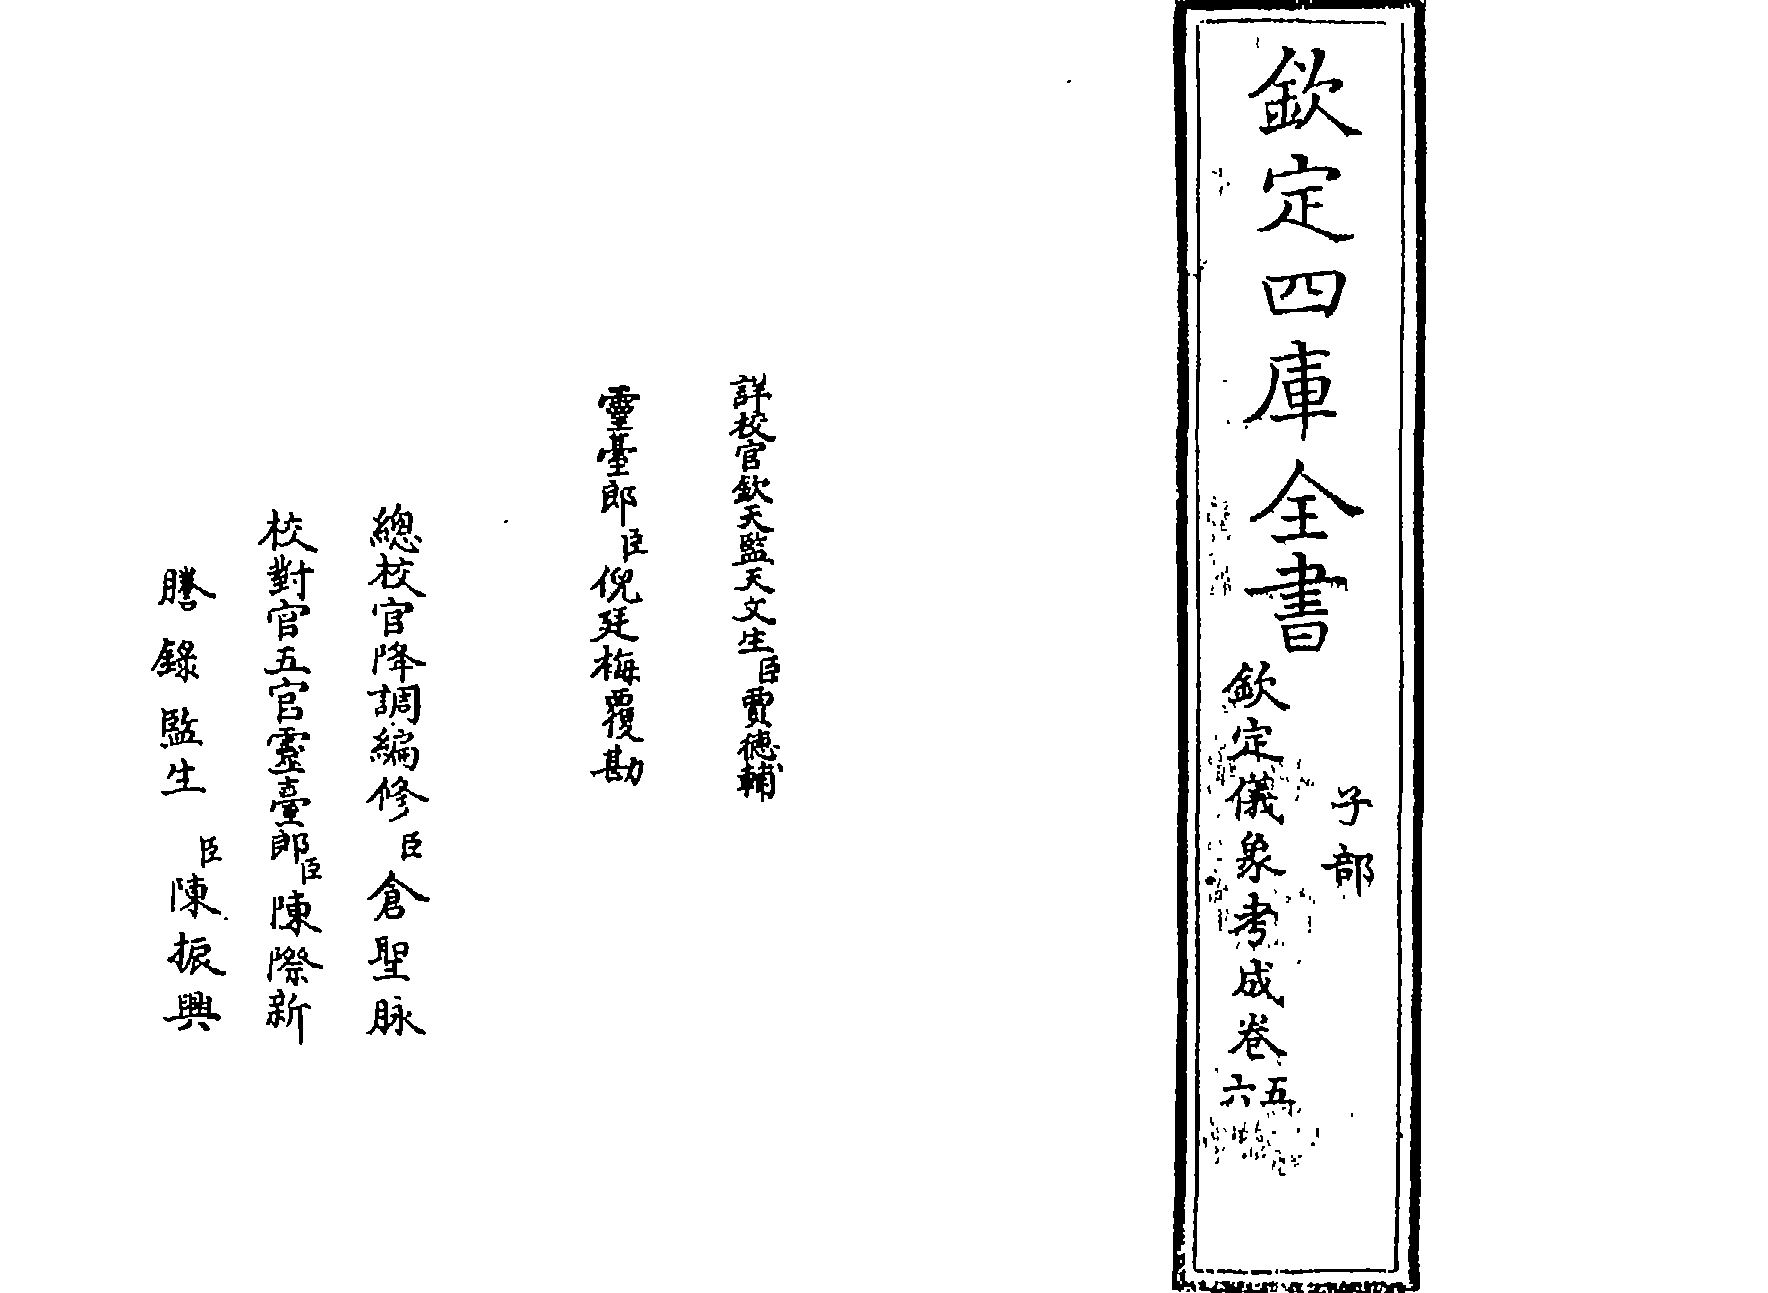
\includegraphics[width=\paperwidth,height=\paperheight,keepaspectratio]{img/0608.png}\clearpage
\begin{正文}
% ---- 册793 葉609 ----
\SetPageNumber{1}
欽定四庫全書\换行
欽定儀象考成卷五\换行
　恒星黄道經緯度表四\换行
　　黄道降婁宫\换行
\char"200B\relax\换行
\char"200B\relax\换行
\char"200B\relax\换行
\char"200B\relax\换行
\char"200B\relax\换行
\char"200B\relax\换行
\char"200B\relax\换行
\char"200B\relax\换行
\char"200B\relax\换行
\char"200B\relax\换行
\char"200B\relax\换行
\char"200B\relax
\par
\end{正文}\clearpage
\嵌图{144.63pt}{201.03pt}{842.50pt}{587.73pt}{img/0612.png}
\begin{正文}
% ---- 册793 葉612 图版 ----
\SetPageNumber{2}
\插图页
\char"200B\relax\换行
\char"200B\relax\换行
\char"200B\relax\换行
\char"200B\relax\换行
\char"200B\relax\换行
\char"200B\relax\换行
\char"200B\relax\换行
\char"200B\relax\换行
\char"200B\relax\换行
\char"200B\relax\换行
\char"200B\relax\换行
\char"200B\relax\换行
\char"200B\relax\换行
\char"200B\relax\换行
\char"200B\relax\换行
\char"200B\relax
\恢复丝栏\par
\end{正文}\clearpage
\嵌图{142.64pt}{201.47pt}{846.47pt}{586.84pt}{img/0613.png}
\begin{正文}
% ---- 册793 葉613 图版 ----
\SetPageNumber{3}
\插图页
\char"200B\relax\换行
\char"200B\relax\换行
\char"200B\relax\换行
\char"200B\relax\换行
\char"200B\relax\换行
\char"200B\relax\换行
\char"200B\relax\换行
\char"200B\relax\换行
\char"200B\relax\换行
\char"200B\relax\换行
\char"200B\relax\换行
\char"200B\relax\换行
\char"200B\relax\换行
\char"200B\relax\换行
\char"200B\relax\换行
\char"200B\relax
\恢复丝栏\par
\end{正文}\clearpage
\嵌图{144.59pt}{201.04pt}{842.59pt}{587.72pt}{img/0616.png}
\begin{正文}
% ---- 册793 葉616 图版 ----
\SetPageNumber{4}
\插图页
\char"200B\relax\换行
\char"200B\relax\换行
\char"200B\relax\换行
\char"200B\relax\换行
\char"200B\relax\换行
\char"200B\relax\换行
\char"200B\relax\换行
\char"200B\relax\换行
\char"200B\relax\换行
\char"200B\relax\换行
\char"200B\relax\换行
\char"200B\relax\换行
\char"200B\relax\换行
\char"200B\relax\换行
\char"200B\relax\换行
\char"200B\relax
\恢复丝栏\par
\end{正文}\clearpage
\嵌图{148.54pt}{201.51pt}{834.68pt}{586.77pt}{img/0617.png}
\begin{正文}
% ---- 册793 葉617 图版 ----
\SetPageNumber{5}
\插图页
\char"200B\relax\换行
\char"200B\relax\换行
\char"200B\relax\换行
\char"200B\relax\换行
\char"200B\relax\换行
\char"200B\relax\换行
\char"200B\relax\换行
\char"200B\relax\换行
\char"200B\relax\换行
\char"200B\relax\换行
\char"200B\relax\换行
\char"200B\relax\换行
\char"200B\relax\换行
\char"200B\relax\换行
\char"200B\relax\换行
\char"200B\relax
\恢复丝栏\par
\end{正文}\clearpage
\嵌图{144.63pt}{201.46pt}{842.50pt}{586.87pt}{img/0620.png}
\begin{正文}
% ---- 册793 葉620 图版 ----
\SetPageNumber{6}
\插图页
\char"200B\relax\换行
\char"200B\relax\换行
\char"200B\relax\换行
\char"200B\relax\换行
\char"200B\relax\换行
\char"200B\relax\换行
\char"200B\relax\换行
\char"200B\relax\换行
\char"200B\relax\换行
\char"200B\relax\换行
\char"200B\relax\换行
\char"200B\relax\换行
\char"200B\relax\换行
\char"200B\relax\换行
\char"200B\relax\换行
\char"200B\relax
\恢复丝栏\par
\end{正文}\clearpage
\嵌图{144.63pt}{201.88pt}{842.50pt}{586.04pt}{img/0621.png}
\begin{正文}
% ---- 册793 葉621 图版 ----
\SetPageNumber{7}
\插图页
\char"200B\relax\换行
\char"200B\relax\换行
\char"200B\relax\换行
\char"200B\relax\换行
\char"200B\relax\换行
\char"200B\relax\换行
\char"200B\relax\换行
\char"200B\relax\换行
\char"200B\relax\换行
\char"200B\relax\换行
\char"200B\relax\换行
\char"200B\relax\换行
\char"200B\relax\换行
\char"200B\relax\换行
\char"200B\relax\换行
\char"200B\relax
\恢复丝栏\par
\end{正文}\clearpage
\嵌图{144.63pt}{202.91pt}{842.50pt}{583.97pt}{img/0624.png}
\begin{正文}
% ---- 册793 葉624 图版 ----
\SetPageNumber{8}
\插图页
\char"200B\relax\换行
\char"200B\relax\换行
\char"200B\relax\换行
\char"200B\relax\换行
\char"200B\relax\换行
\char"200B\relax\换行
\char"200B\relax\换行
\char"200B\relax\换行
\char"200B\relax\换行
\char"200B\relax\换行
\char"200B\relax\换行
\char"200B\relax\换行
\char"200B\relax\换行
\char"200B\relax\换行
\char"200B\relax\换行
\char"200B\relax
\恢复丝栏\par
\end{正文}\clearpage
\嵌图{146.62pt}{203.36pt}{838.53pt}{583.08pt}{img/0625.png}
\begin{正文}
% ---- 册793 葉625 图版 ----
\SetPageNumber{9}
\插图页
\char"200B\relax\换行
\char"200B\relax\换行
\char"200B\relax\换行
\char"200B\relax\换行
\char"200B\relax\换行
\char"200B\relax\换行
\char"200B\relax\换行
\char"200B\relax\换行
\char"200B\relax\换行
\char"200B\relax\换行
\char"200B\relax\换行
\char"200B\relax\换行
\char"200B\relax\换行
\char"200B\relax\换行
\char"200B\relax\换行
\char"200B\relax
\恢复丝栏\par
\end{正文}\clearpage
\嵌图{148.54pt}{201.88pt}{834.68pt}{586.02pt}{img/0628.png}
\begin{正文}
% ---- 册793 葉628 图版 ----
\SetPageNumber{10}
\插图页
\char"200B\relax\换行
\char"200B\relax\换行
\char"200B\relax\换行
\char"200B\relax\换行
\char"200B\relax\换行
\char"200B\relax\换行
\char"200B\relax\换行
\char"200B\relax\换行
\char"200B\relax\换行
\char"200B\relax\换行
\char"200B\relax\换行
\char"200B\relax\换行
\char"200B\relax\换行
\char"200B\relax\换行
\char"200B\relax\换行
\char"200B\relax
\恢复丝栏\par
\end{正文}\clearpage
\嵌图{146.56pt}{200.93pt}{838.64pt}{587.93pt}{img/0629.png}
\begin{正文}
% ---- 册793 葉629 图版 ----
\SetPageNumber{11}
\插图页
\char"200B\relax\换行
\char"200B\relax\换行
\char"200B\relax\换行
\char"200B\relax\换行
\char"200B\relax\换行
\char"200B\relax\换行
\char"200B\relax\换行
\char"200B\relax\换行
\char"200B\relax\换行
\char"200B\relax\换行
\char"200B\relax\换行
\char"200B\relax\换行
\char"200B\relax\换行
\char"200B\relax\换行
\char"200B\relax\换行
\char"200B\relax
\恢复丝栏\par
\end{正文}\clearpage
\嵌图{142.64pt}{201.95pt}{846.47pt}{585.90pt}{img/0632.png}
\begin{正文}
% ---- 册793 葉632 图版 ----
\SetPageNumber{12}
\插图页
\char"200B\relax\换行
\char"200B\relax\换行
\char"200B\relax\换行
\char"200B\relax\换行
\char"200B\relax\换行
\char"200B\relax\换行
\char"200B\relax\换行
\char"200B\relax\换行
\char"200B\relax\换行
\char"200B\relax\换行
\char"200B\relax\换行
\char"200B\relax\换行
\char"200B\relax\换行
\char"200B\relax\换行
\char"200B\relax\换行
\char"200B\relax
\恢复丝栏\par
\end{正文}\clearpage
\嵌图{144.63pt}{200.54pt}{842.50pt}{588.72pt}{img/0633.png}
\begin{正文}
% ---- 册793 葉633 图版 ----
\SetPageNumber{13}
\插图页
\char"200B\relax\换行
\char"200B\relax\换行
\char"200B\relax\换行
\char"200B\relax\换行
\char"200B\relax\换行
\char"200B\relax\换行
\char"200B\relax\换行
\char"200B\relax\换行
\char"200B\relax\换行
\char"200B\relax\换行
\char"200B\relax\换行
\char"200B\relax\换行
\char"200B\relax\换行
\char"200B\relax\换行
\char"200B\relax\换行
\char"200B\relax
\恢复丝栏\par
\end{正文}\clearpage
\嵌图{144.63pt}{200.93pt}{842.50pt}{587.93pt}{img/0636.png}
\begin{正文}
% ---- 册793 葉636 图版 ----
\SetPageNumber{14}
\插图页
\char"200B\relax\换行
\char"200B\relax\换行
\char"200B\relax\换行
\char"200B\relax\换行
\char"200B\relax\换行
\char"200B\relax\换行
\char"200B\relax\换行
\char"200B\relax\换行
\char"200B\relax\换行
\char"200B\relax\换行
\char"200B\relax\换行
\char"200B\relax\换行
\char"200B\relax\换行
\char"200B\relax\换行
\char"200B\relax\换行
\char"200B\relax
\恢复丝栏\par
\end{正文}\clearpage
\嵌图{148.61pt}{199.50pt}{834.55pt}{590.78pt}{img/0637.png}
\begin{正文}
% ---- 册793 葉637 图版 ----
\SetPageNumber{15}
\插图页
\char"200B\relax\换行
\char"200B\relax\换行
\char"200B\relax\换行
\char"200B\relax\换行
\char"200B\relax\换行
\char"200B\relax\换行
\char"200B\relax\换行
\char"200B\relax\换行
\char"200B\relax\换行
\char"200B\relax\换行
\char"200B\relax\换行
\char"200B\relax\换行
\char"200B\relax\换行
\char"200B\relax\换行
\char"200B\relax\换行
\char"200B\relax
\恢复丝栏\par
\end{正文}\clearpage
\嵌图{144.63pt}{201.95pt}{842.50pt}{585.90pt}{img/0640.png}
\begin{正文}
% ---- 册793 葉640 图版 ----
\SetPageNumber{16}
\插图页
\char"200B\relax\换行
\char"200B\relax\换行
\char"200B\relax\换行
\char"200B\relax\换行
\char"200B\relax\换行
\char"200B\relax\换行
\char"200B\relax\换行
\char"200B\relax\换行
\char"200B\relax\换行
\char"200B\relax\换行
\char"200B\relax\换行
\char"200B\relax\换行
\char"200B\relax\换行
\char"200B\relax\换行
\char"200B\relax\换行
\char"200B\relax
\恢复丝栏\par
\end{正文}\clearpage
\嵌图{144.63pt}{201.02pt}{842.50pt}{587.76pt}{img/0641.png}
\begin{正文}
% ---- 册793 葉641 图版 ----
\SetPageNumber{17}
\插图页
\char"200B\relax\换行
\char"200B\relax\换行
\char"200B\relax\换行
\char"200B\relax\换行
\char"200B\relax\换行
\char"200B\relax\换行
\char"200B\relax\换行
\char"200B\relax\换行
\char"200B\relax\换行
\char"200B\relax\换行
\char"200B\relax\换行
\char"200B\relax\换行
\char"200B\relax\换行
\char"200B\relax\换行
\char"200B\relax\换行
\char"200B\relax
\恢复丝栏\par
\end{正文}\clearpage
\嵌图{146.67pt}{200.52pt}{838.42pt}{588.75pt}{img/0644.png}
\begin{正文}
% ---- 册793 葉644 图版 ----
\SetPageNumber{18}
\插图页
\char"200B\relax\换行
\char"200B\relax\换行
\char"200B\relax\换行
\char"200B\relax\换行
\char"200B\relax\换行
\char"200B\relax\换行
\char"200B\relax\换行
\char"200B\relax\换行
\char"200B\relax\换行
\char"200B\relax\换行
\char"200B\relax\换行
\char"200B\relax\换行
\char"200B\relax\换行
\char"200B\relax\换行
\char"200B\relax\换行
\char"200B\relax
\恢复丝栏\par
\end{正文}\clearpage
\嵌图{150.67pt}{200.99pt}{830.43pt}{587.80pt}{img/0645.png}
\begin{正文}
% ---- 册793 葉645 图版 ----
\SetPageNumber{19}
\插图页
\char"200B\relax\换行
\char"200B\relax\换行
\char"200B\relax\换行
\char"200B\relax\换行
\char"200B\relax\换行
\char"200B\relax\换行
\char"200B\relax\换行
\char"200B\relax\换行
\char"200B\relax\换行
\char"200B\relax\换行
\char"200B\relax\换行
\char"200B\relax\换行
\char"200B\relax\换行
\char"200B\relax\换行
\char"200B\relax\换行
\char"200B\relax
\恢复丝栏\par
\end{正文}\clearpage
\嵌图{140.63pt}{199.98pt}{850.50pt}{589.83pt}{img/0648.png}
\begin{正文}
% ---- 册793 葉648 图版 ----
\SetPageNumber{20}
\插图页
\char"200B\relax\换行
\char"200B\relax\换行
\char"200B\relax\换行
\char"200B\relax\换行
\char"200B\relax\换行
\char"200B\relax\换行
\char"200B\relax\换行
\char"200B\relax\换行
\char"200B\relax\换行
\char"200B\relax\换行
\char"200B\relax\换行
\char"200B\relax\换行
\char"200B\relax\换行
\char"200B\relax\换行
\char"200B\relax\换行
\char"200B\relax
\恢复丝栏\par
\end{正文}\clearpage
\嵌图{146.56pt}{200.49pt}{838.64pt}{588.82pt}{img/0649.png}
\begin{正文}
% ---- 册793 葉649 图版 ----
\SetPageNumber{21}
\插图页
\char"200B\relax\换行
\char"200B\relax\换行
\char"200B\relax\换行
\char"200B\relax\换行
\char"200B\relax\换行
\char"200B\relax\换行
\char"200B\relax\换行
\char"200B\relax\换行
\char"200B\relax\换行
\char"200B\relax\换行
\char"200B\relax\换行
\char"200B\relax\换行
\char"200B\relax\换行
\char"200B\relax\换行
\char"200B\relax\换行
\char"200B\relax
\恢复丝栏\par
\end{正文}\clearpage
\嵌图{126.91pt}{215.07pt}{762.93pt}{577.76pt}{img/0652.png}
\begin{正文}
% ---- 册793 葉652 ----
\SetPageNumber{22}
\插图页
\char"200B\relax\换行
\char"200B\relax\换行
\char"200B\relax\换行
\char"200B\relax\换行
\char"200B\relax\换行
\char"200B\relax\换行
\char"200B\relax\换行
\char"200B\relax\换行
\恢复丝栏
\char"200B\relax\换行
\char"200B\relax\换行
\char"200B\relax\换行
\char"200B\relax\换行
\char"200B\relax\换行
\char"200B\relax\换行
欽定儀象考成卷五\换行
\char"200B\relax
\par

% ======== 卷六（8行21字）========
\par\end{正文}\clearpage
\chapter*{欽定儀象考成卷六}
\begin{正文}
% ---- 册793 葉653 ----
\SetPageNumber{1}
欽定四庫全書\换行
欽定儀象考成卷六\换行
　恒星黄道經緯度表五\换行
　　黄道大梁宫\双列{\右小列{赤道度附}\左小列{}}\换行
\char"200B\relax\换行
\char"200B\relax\换行
\char"200B\relax\换行
\char"200B\relax\换行
\char"200B\relax\换行
\char"200B\relax\换行
\char"200B\relax\换行
\char"200B\relax\换行
\char"200B\relax\换行
\char"200B\relax\换行
\char"200B\relax\换行
\char"200B\relax
\par
\end{正文}\clearpage
\嵌图{142.68pt}{198.67pt}{846.40pt}{592.45pt}{img/0656.png}
\begin{正文}
% ---- 册793 葉656 图版 ----
\SetPageNumber{2}
\插图页
\char"200B\relax\换行
\char"200B\relax\换行
\char"200B\relax\换行
\char"200B\relax\换行
\char"200B\relax\换行
\char"200B\relax\换行
\char"200B\relax\换行
\char"200B\relax\换行
\char"200B\relax\换行
\char"200B\relax\换行
\char"200B\relax\换行
\char"200B\relax\换行
\char"200B\relax\换行
\char"200B\relax\换行
\char"200B\relax\换行
\char"200B\relax
\恢复丝栏\par
\end{正文}\clearpage
\嵌图{146.67pt}{203.90pt}{838.42pt}{582.00pt}{img/0657.png}
\begin{正文}
% ---- 册793 葉657 图版 ----
\SetPageNumber{3}
\插图页
\char"200B\relax\换行
\char"200B\relax\换行
\char"200B\relax\换行
\char"200B\relax\换行
\char"200B\relax\换行
\char"200B\relax\换行
\char"200B\relax\换行
\char"200B\relax\换行
\char"200B\relax\换行
\char"200B\relax\换行
\char"200B\relax\换行
\char"200B\relax\换行
\char"200B\relax\换行
\char"200B\relax\换行
\char"200B\relax\换行
\char"200B\relax
\恢复丝栏\par
\end{正文}\clearpage
\嵌图{148.61pt}{201.92pt}{834.55pt}{585.94pt}{img/0660.png}
\begin{正文}
% ---- 册793 葉660 图版 ----
\SetPageNumber{4}
\插图页
\char"200B\relax\换行
\char"200B\relax\换行
\char"200B\relax\换行
\char"200B\relax\换行
\char"200B\relax\换行
\char"200B\relax\换行
\char"200B\relax\换行
\char"200B\relax\换行
\char"200B\relax\换行
\char"200B\relax\换行
\char"200B\relax\换行
\char"200B\relax\换行
\char"200B\relax\换行
\char"200B\relax\换行
\char"200B\relax\换行
\char"200B\relax
\恢复丝栏\par
\end{正文}\clearpage
\嵌图{146.62pt}{201.41pt}{838.53pt}{586.96pt}{img/0661.png}
\begin{正文}
% ---- 册793 葉661 图版 ----
\SetPageNumber{5}
\插图页
\char"200B\relax\换行
\char"200B\relax\换行
\char"200B\relax\换行
\char"200B\relax\换行
\char"200B\relax\换行
\char"200B\relax\换行
\char"200B\relax\换行
\char"200B\relax\换行
\char"200B\relax\换行
\char"200B\relax\换行
\char"200B\relax\换行
\char"200B\relax\换行
\char"200B\relax\换行
\char"200B\relax\换行
\char"200B\relax\换行
\char"200B\relax
\恢复丝栏\par
\end{正文}\clearpage
\嵌图{146.67pt}{201.55pt}{838.42pt}{586.69pt}{img/0664.png}
\begin{正文}
% ---- 册793 葉664 图版 ----
\SetPageNumber{6}
\插图页
\char"200B\relax\换行
\char"200B\relax\换行
\char"200B\relax\换行
\char"200B\relax\换行
\char"200B\relax\换行
\char"200B\relax\换行
\char"200B\relax\换行
\char"200B\relax\换行
\char"200B\relax\换行
\char"200B\relax\换行
\char"200B\relax\换行
\char"200B\relax\换行
\char"200B\relax\换行
\char"200B\relax\换行
\char"200B\relax\换行
\char"200B\relax
\恢复丝栏\par
\end{正文}\clearpage
\嵌图{144.68pt}{200.53pt}{842.41pt}{588.73pt}{img/0665.png}
\begin{正文}
% ---- 册793 葉665 图版 ----
\SetPageNumber{7}
\插图页
\char"200B\relax\换行
\char"200B\relax\换行
\char"200B\relax\换行
\char"200B\relax\换行
\char"200B\relax\换行
\char"200B\relax\换行
\char"200B\relax\换行
\char"200B\relax\换行
\char"200B\relax\换行
\char"200B\relax\换行
\char"200B\relax\换行
\char"200B\relax\换行
\char"200B\relax\换行
\char"200B\relax\换行
\char"200B\relax\换行
\char"200B\relax
\恢复丝栏\par
\end{正文}\clearpage
\嵌图{146.67pt}{200.50pt}{838.42pt}{588.79pt}{img/0668.png}
\begin{正文}
% ---- 册793 葉668 图版 ----
\SetPageNumber{8}
\插图页
\char"200B\relax\换行
\char"200B\relax\换行
\char"200B\relax\换行
\char"200B\relax\换行
\char"200B\relax\换行
\char"200B\relax\换行
\char"200B\relax\换行
\char"200B\relax\换行
\char"200B\relax\换行
\char"200B\relax\换行
\char"200B\relax\换行
\char"200B\relax\换行
\char"200B\relax\换行
\char"200B\relax\换行
\char"200B\relax\换行
\char"200B\relax
\恢复丝栏\par
\end{正文}\clearpage
\嵌图{148.67pt}{199.52pt}{834.42pt}{590.75pt}{img/0669.png}
\begin{正文}
% ---- 册793 葉669 图版 ----
\SetPageNumber{9}
\插图页
\char"200B\relax\换行
\char"200B\relax\换行
\char"200B\relax\换行
\char"200B\relax\换行
\char"200B\relax\换行
\char"200B\relax\换行
\char"200B\relax\换行
\char"200B\relax\换行
\char"200B\relax\换行
\char"200B\relax\换行
\char"200B\relax\换行
\char"200B\relax\换行
\char"200B\relax\换行
\char"200B\relax\换行
\char"200B\relax\换行
\char"200B\relax
\恢复丝栏\par
\end{正文}\clearpage
\嵌图{144.63pt}{201.94pt}{842.50pt}{585.91pt}{img/0672.png}
\begin{正文}
% ---- 册793 葉672 图版 ----
\SetPageNumber{10}
\插图页
\char"200B\relax\换行
\char"200B\relax\换行
\char"200B\relax\换行
\char"200B\relax\换行
\char"200B\relax\换行
\char"200B\relax\换行
\char"200B\relax\换行
\char"200B\relax\换行
\char"200B\relax\换行
\char"200B\relax\换行
\char"200B\relax\换行
\char"200B\relax\换行
\char"200B\relax\换行
\char"200B\relax\换行
\char"200B\relax\换行
\char"200B\relax
\恢复丝栏\par
\end{正文}\clearpage
\嵌图{144.63pt}{202.90pt}{842.50pt}{583.99pt}{img/0673.png}
\begin{正文}
% ---- 册793 葉673 图版 ----
\SetPageNumber{11}
\插图页
\char"200B\relax\换行
\char"200B\relax\换行
\char"200B\relax\换行
\char"200B\relax\换行
\char"200B\relax\换行
\char"200B\relax\换行
\char"200B\relax\换行
\char"200B\relax\换行
\char"200B\relax\换行
\char"200B\relax\换行
\char"200B\relax\换行
\char"200B\relax\换行
\char"200B\relax\换行
\char"200B\relax\换行
\char"200B\relax\换行
\char"200B\relax
\恢复丝栏\par
\end{正文}\clearpage
\嵌图{148.73pt}{201.95pt}{834.29pt}{585.88pt}{img/0676.png}
\begin{正文}
% ---- 册793 葉676 图版 ----
\SetPageNumber{12}
\插图页
\char"200B\relax\换行
\char"200B\relax\换行
\char"200B\relax\换行
\char"200B\relax\换行
\char"200B\relax\换行
\char"200B\relax\换行
\char"200B\relax\换行
\char"200B\relax\换行
\char"200B\relax\换行
\char"200B\relax\换行
\char"200B\relax\换行
\char"200B\relax\换行
\char"200B\relax\换行
\char"200B\relax\换行
\char"200B\relax\换行
\char"200B\relax
\恢复丝栏\par
\end{正文}\clearpage
\嵌图{146.73pt}{198.17pt}{838.30pt}{593.45pt}{img/0677.png}
\begin{正文}
% ---- 册793 葉677 图版 ----
\SetPageNumber{13}
\插图页
\char"200B\relax\换行
\char"200B\relax\换行
\char"200B\relax\换行
\char"200B\relax\换行
\char"200B\relax\换行
\char"200B\relax\换行
\char"200B\relax\换行
\char"200B\relax\换行
\char"200B\relax\换行
\char"200B\relax\换行
\char"200B\relax\换行
\char"200B\relax\换行
\char"200B\relax\换行
\char"200B\relax\换行
\char"200B\relax\换行
\char"200B\relax
\恢复丝栏\par
\end{正文}\clearpage
\嵌图{146.56pt}{202.90pt}{838.64pt}{583.99pt}{img/0680.png}
\begin{正文}
% ---- 册793 葉680 图版 ----
\SetPageNumber{14}
\插图页
\char"200B\relax\换行
\char"200B\relax\换行
\char"200B\relax\换行
\char"200B\relax\换行
\char"200B\relax\换行
\char"200B\relax\换行
\char"200B\relax\换行
\char"200B\relax\换行
\char"200B\relax\换行
\char"200B\relax\换行
\char"200B\relax\换行
\char"200B\relax\换行
\char"200B\relax\换行
\char"200B\relax\换行
\char"200B\relax\换行
\char"200B\relax
\恢复丝栏\par
\end{正文}\clearpage
\嵌图{148.54pt}{205.26pt}{834.68pt}{579.28pt}{img/0681.png}
\begin{正文}
% ---- 册793 葉681 图版 ----
\SetPageNumber{15}
\插图页
\char"200B\relax\换行
\char"200B\relax\换行
\char"200B\relax\换行
\char"200B\relax\换行
\char"200B\relax\换行
\char"200B\relax\换行
\char"200B\relax\换行
\char"200B\relax\换行
\char"200B\relax\换行
\char"200B\relax\换行
\char"200B\relax\换行
\char"200B\relax\换行
\char"200B\relax\换行
\char"200B\relax\换行
\char"200B\relax\换行
\char"200B\relax
\恢复丝栏\par
\end{正文}\clearpage
\嵌图{146.56pt}{203.84pt}{838.64pt}{582.11pt}{img/0684.png}
\begin{正文}
% ---- 册793 葉684 图版 ----
\SetPageNumber{16}
\插图页
\char"200B\relax\换行
\char"200B\relax\换行
\char"200B\relax\换行
\char"200B\relax\换行
\char"200B\relax\换行
\char"200B\relax\换行
\char"200B\relax\换行
\char"200B\relax\换行
\char"200B\relax\换行
\char"200B\relax\换行
\char"200B\relax\换行
\char"200B\relax\换行
\char"200B\relax\换行
\char"200B\relax\换行
\char"200B\relax\换行
\char"200B\relax
\恢复丝栏\par
\end{正文}\clearpage
\嵌图{146.56pt}{200.49pt}{838.64pt}{588.80pt}{img/0685.png}
\begin{正文}
% ---- 册793 葉685 图版 ----
\SetPageNumber{17}
\插图页
\char"200B\relax\换行
\char"200B\relax\换行
\char"200B\relax\换行
\char"200B\relax\换行
\char"200B\relax\换行
\char"200B\relax\换行
\char"200B\relax\换行
\char"200B\relax\换行
\char"200B\relax\换行
\char"200B\relax\换行
\char"200B\relax\换行
\char"200B\relax\换行
\char"200B\relax\换行
\char"200B\relax\换行
\char"200B\relax\换行
\char"200B\relax
\恢复丝栏\par
\end{正文}\clearpage
\嵌图{140.68pt}{203.93pt}{850.39pt}{581.92pt}{img/0688.png}
\begin{正文}
% ---- 册793 葉688 图版 ----
\SetPageNumber{18}
\插图页
\char"200B\relax\换行
\char"200B\relax\换行
\char"200B\relax\换行
\char"200B\relax\换行
\char"200B\relax\换行
\char"200B\relax\换行
\char"200B\relax\换行
\char"200B\relax\换行
\char"200B\relax\换行
\char"200B\relax\换行
\char"200B\relax\换行
\char"200B\relax\换行
\char"200B\relax\换行
\char"200B\relax\换行
\char"200B\relax\换行
\char"200B\relax
\恢复丝栏\par
\end{正文}\clearpage
\嵌图{150.67pt}{200.58pt}{830.43pt}{588.62pt}{img/0689.png}
\begin{正文}
% ---- 册793 葉689 图版 ----
\SetPageNumber{19}
\插图页
\char"200B\relax\换行
\char"200B\relax\换行
\char"200B\relax\换行
\char"200B\relax\换行
\char"200B\relax\换行
\char"200B\relax\换行
\char"200B\relax\换行
\char"200B\relax\换行
\char"200B\relax\换行
\char"200B\relax\换行
\char"200B\relax\换行
\char"200B\relax\换行
\char"200B\relax\换行
\char"200B\relax\换行
\char"200B\relax\换行
\char"200B\relax
\恢复丝栏\par
\end{正文}\clearpage
\嵌图{148.61pt}{201.93pt}{834.55pt}{585.93pt}{img/0692.png}
\begin{正文}
% ---- 册793 葉692 图版 ----
\SetPageNumber{20}
\插图页
\char"200B\relax\换行
\char"200B\relax\换行
\char"200B\relax\换行
\char"200B\relax\换行
\char"200B\relax\换行
\char"200B\relax\换行
\char"200B\relax\换行
\char"200B\relax\换行
\char"200B\relax\换行
\char"200B\relax\换行
\char"200B\relax\换行
\char"200B\relax\换行
\char"200B\relax\换行
\char"200B\relax\换行
\char"200B\relax\换行
\char"200B\relax
\恢复丝栏\par
\end{正文}\clearpage
\嵌图{146.62pt}{204.25pt}{838.53pt}{581.28pt}{img/0693.png}
\begin{正文}
% ---- 册793 葉693 图版 ----
\SetPageNumber{21}
\插图页
\char"200B\relax\换行
\char"200B\relax\换行
\char"200B\relax\换行
\char"200B\relax\换行
\char"200B\relax\换行
\char"200B\relax\换行
\char"200B\relax\换行
\char"200B\relax\换行
\char"200B\relax\换行
\char"200B\relax\换行
\char"200B\relax\换行
\char"200B\relax\换行
\char"200B\relax\换行
\char"200B\relax\换行
\char"200B\relax\换行
\char"200B\relax
\恢复丝栏\par
\end{正文}\clearpage
\嵌图{144.72pt}{203.93pt}{842.31pt}{581.92pt}{img/0696.png}
\begin{正文}
% ---- 册793 葉696 图版 ----
\SetPageNumber{22}
\插图页
\char"200B\relax\换行
\char"200B\relax\换行
\char"200B\relax\换行
\char"200B\relax\换行
\char"200B\relax\换行
\char"200B\relax\换行
\char"200B\relax\换行
\char"200B\relax\换行
\char"200B\relax\换行
\char"200B\relax\换行
\char"200B\relax\换行
\char"200B\relax\换行
\char"200B\relax\换行
\char"200B\relax\换行
\char"200B\relax\换行
\char"200B\relax
\恢复丝栏\par
\end{正文}\clearpage
\嵌图{164.65pt}{222.62pt}{725.19pt}{570.21pt}{img/0697.png}
\begin{正文}
% ---- 册793 葉697 ----
\SetPageNumber{23}
\插图页
\char"200B\relax\换行
\char"200B\relax\换行
\char"200B\relax\换行
\char"200B\relax\换行
\char"200B\relax\换行
\char"200B\relax\换行
\char"200B\relax\换行
\char"200B\relax\换行
\恢复丝栏
\char"200B\relax\换行
\char"200B\relax\换行
\char"200B\relax\换行
\char"200B\relax\换行
\char"200B\relax\换行
\char"200B\relax\换行
\char"200B\relax\换行
欽定儀象考成卷六
\par

\par\end{正文}\clearpage

  \input{parts/part07}
  \thispagestyle{empty}\noindent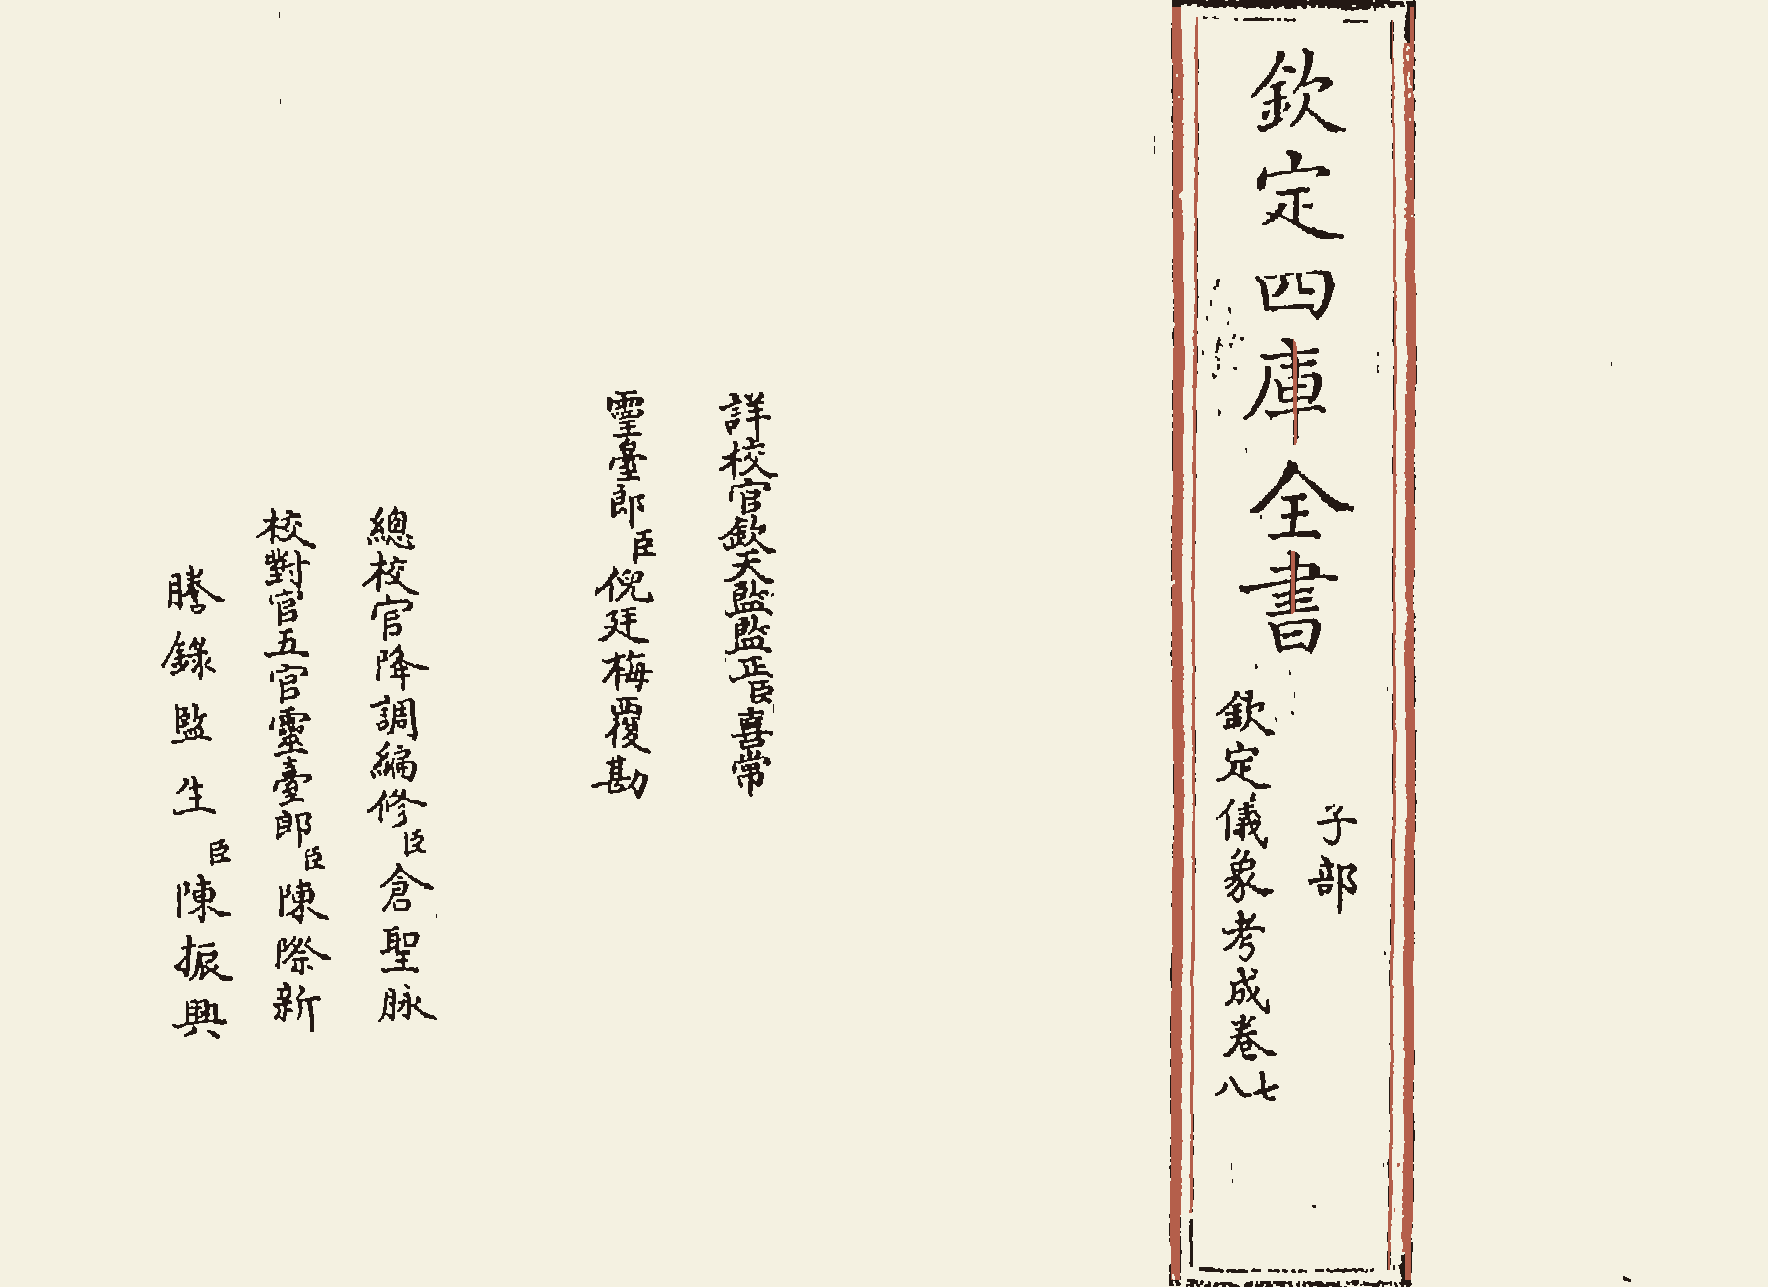
\includegraphics[width=\paperwidth,height=\paperheight,keepaspectratio]{img/0700.png}\clearpage
\begin{正文}
% ---- 册793 葉701 ----
\SetPageNumber{1}
欽定四庫全書\换行
欽定儀象考成卷七\换行
　恒星黄道經緯度表六\换行
　　黄道實沈宫\双列{\右小列{赤道度附}\左小列{}}\换行
\char"200B\relax\换行
\char"200B\relax\换行
\char"200B\relax\换行
\char"200B\relax\换行
\char"200B\relax\换行
\char"200B\relax\换行
\char"200B\relax\换行
\char"200B\relax\换行
\char"200B\relax\换行
\char"200B\relax\换行
\char"200B\relax\换行
\char"200B\relax
\par
\end{正文}\clearpage
\嵌图{146.56pt}{202.48pt}{838.64pt}{584.83pt}{img/0704.png}
\begin{正文}
% ---- 册793 葉704 图版 ----
\SetPageNumber{2}
\插图页
\char"200B\relax\换行
\char"200B\relax\换行
\char"200B\relax\换行
\char"200B\relax\换行
\char"200B\relax\换行
\char"200B\relax\换行
\char"200B\relax\换行
\char"200B\relax\换行
\char"200B\relax\换行
\char"200B\relax\换行
\char"200B\relax\换行
\char"200B\relax\换行
\char"200B\relax\换行
\char"200B\relax\换行
\char"200B\relax\换行
\char"200B\relax
\恢复丝栏\par
\end{正文}\clearpage
\嵌图{148.54pt}{201.50pt}{834.68pt}{586.80pt}{img/0705.png}
\begin{正文}
% ---- 册793 葉705 图版 ----
\SetPageNumber{3}
\插图页
\char"200B\relax\换行
\char"200B\relax\换行
\char"200B\relax\换行
\char"200B\relax\换行
\char"200B\relax\换行
\char"200B\relax\换行
\char"200B\relax\换行
\char"200B\relax\换行
\char"200B\relax\换行
\char"200B\relax\换行
\char"200B\relax\换行
\char"200B\relax\换行
\char"200B\relax\换行
\char"200B\relax\换行
\char"200B\relax\换行
\char"200B\relax
\恢复丝栏\par
\end{正文}\clearpage
\嵌图{146.62pt}{203.90pt}{838.53pt}{582.00pt}{img/0708.png}
\begin{正文}
% ---- 册793 葉708 图版 ----
\SetPageNumber{4}
\插图页
\char"200B\relax\换行
\char"200B\relax\换行
\char"200B\relax\换行
\char"200B\relax\换行
\char"200B\relax\换行
\char"200B\relax\换行
\char"200B\relax\换行
\char"200B\relax\换行
\char"200B\relax\换行
\char"200B\relax\换行
\char"200B\relax\换行
\char"200B\relax\换行
\char"200B\relax\换行
\char"200B\relax\换行
\char"200B\relax\换行
\char"200B\relax
\恢复丝栏\par
\end{正文}\clearpage
\嵌图{144.63pt}{200.99pt}{842.50pt}{587.82pt}{img/0709.png}
\begin{正文}
% ---- 册793 葉709 图版 ----
\SetPageNumber{5}
\插图页
\char"200B\relax\换行
\char"200B\relax\换行
\char"200B\relax\换行
\char"200B\relax\换行
\char"200B\relax\换行
\char"200B\relax\换行
\char"200B\relax\换行
\char"200B\relax\换行
\char"200B\relax\换行
\char"200B\relax\换行
\char"200B\relax\换行
\char"200B\relax\换行
\char"200B\relax\换行
\char"200B\relax\换行
\char"200B\relax\换行
\char"200B\relax
\恢复丝栏\par
\end{正文}\clearpage
\嵌图{140.66pt}{204.85pt}{850.45pt}{580.10pt}{img/0712.png}
\begin{正文}
% ---- 册793 葉712 图版 ----
\SetPageNumber{6}
\插图页
\char"200B\relax\换行
\char"200B\relax\换行
\char"200B\relax\换行
\char"200B\relax\换行
\char"200B\relax\换行
\char"200B\relax\换行
\char"200B\relax\换行
\char"200B\relax\换行
\char"200B\relax\换行
\char"200B\relax\换行
\char"200B\relax\换行
\char"200B\relax\换行
\char"200B\relax\换行
\char"200B\relax\换行
\char"200B\relax\换行
\char"200B\relax
\恢复丝栏\par
\end{正文}\clearpage
\嵌图{142.64pt}{204.81pt}{846.47pt}{580.16pt}{img/0713.png}
\begin{正文}
% ---- 册793 葉713 图版 ----
\SetPageNumber{7}
\插图页
\char"200B\relax\换行
\char"200B\relax\换行
\char"200B\relax\换行
\char"200B\relax\换行
\char"200B\relax\换行
\char"200B\relax\换行
\char"200B\relax\换行
\char"200B\relax\换行
\char"200B\relax\换行
\char"200B\relax\换行
\char"200B\relax\换行
\char"200B\relax\换行
\char"200B\relax\换行
\char"200B\relax\换行
\char"200B\relax\换行
\char"200B\relax
\恢复丝栏\par
\end{正文}\clearpage
\嵌图{148.54pt}{198.60pt}{834.68pt}{592.58pt}{img/0716.png}
\begin{正文}
% ---- 册793 葉716 图版 ----
\SetPageNumber{8}
\插图页
\char"200B\relax\换行
\char"200B\relax\换行
\char"200B\relax\换行
\char"200B\relax\换行
\char"200B\relax\换行
\char"200B\relax\换行
\char"200B\relax\换行
\char"200B\relax\换行
\char"200B\relax\换行
\char"200B\relax\换行
\char"200B\relax\换行
\char"200B\relax\换行
\char"200B\relax\换行
\char"200B\relax\换行
\char"200B\relax\换行
\char"200B\relax
\恢复丝栏\par
\end{正文}\clearpage
\嵌图{150.52pt}{200.46pt}{830.72pt}{588.87pt}{img/0717.png}
\begin{正文}
% ---- 册793 葉717 图版 ----
\SetPageNumber{9}
\插图页
\char"200B\relax\换行
\char"200B\relax\换行
\char"200B\relax\换行
\char"200B\relax\换行
\char"200B\relax\换行
\char"200B\relax\换行
\char"200B\relax\换行
\char"200B\relax\换行
\char"200B\relax\换行
\char"200B\relax\换行
\char"200B\relax\换行
\char"200B\relax\换行
\char"200B\relax\换行
\char"200B\relax\换行
\char"200B\relax\换行
\char"200B\relax
\恢复丝栏\par
\end{正文}\clearpage
\嵌图{142.64pt}{200.54pt}{846.47pt}{588.72pt}{img/0720.png}
\begin{正文}
% ---- 册793 葉720 图版 ----
\SetPageNumber{10}
\插图页
\char"200B\relax\换行
\char"200B\relax\换行
\char"200B\relax\换行
\char"200B\relax\换行
\char"200B\relax\换行
\char"200B\relax\换行
\char"200B\relax\换行
\char"200B\relax\换行
\char"200B\relax\换行
\char"200B\relax\换行
\char"200B\relax\换行
\char"200B\relax\换行
\char"200B\relax\换行
\char"200B\relax\换行
\char"200B\relax\换行
\char"200B\relax
\恢复丝栏\par
\end{正文}\clearpage
\嵌图{150.59pt}{203.37pt}{830.58pt}{583.06pt}{img/0721.png}
\begin{正文}
% ---- 册793 葉721 图版 ----
\SetPageNumber{11}
\插图页
\char"200B\relax\换行
\char"200B\relax\换行
\char"200B\relax\换行
\char"200B\relax\换行
\char"200B\relax\换行
\char"200B\relax\换行
\char"200B\relax\换行
\char"200B\relax\换行
\char"200B\relax\换行
\char"200B\relax\换行
\char"200B\relax\换行
\char"200B\relax\换行
\char"200B\relax\换行
\char"200B\relax\换行
\char"200B\relax\换行
\char"200B\relax
\恢复丝栏\par
\end{正文}\clearpage
\嵌图{365.19pt}{199.32pt}{401.38pt}{591.16pt}{img/0724.png}
\begin{正文}
% ---- 册793 葉724 图版 ----
\SetPageNumber{12}
\插图页
\char"200B\relax\换行
\char"200B\relax\换行
\char"200B\relax\换行
\char"200B\relax\换行
\char"200B\relax\换行
\char"200B\relax\换行
\char"200B\relax\换行
\char"200B\relax\换行
\char"200B\relax\换行
\char"200B\relax\换行
\char"200B\relax\换行
\char"200B\relax\换行
\char"200B\relax\换行
\char"200B\relax\换行
\char"200B\relax\换行
\char"200B\relax
\恢复丝栏\par
\end{正文}\clearpage
\嵌图{363.20pt}{202.59pt}{405.35pt}{584.61pt}{img/0725.png}
\begin{正文}
% ---- 册793 葉725 图版 ----
\SetPageNumber{13}
\插图页
\char"200B\relax\换行
\char"200B\relax\换行
\char"200B\relax\换行
\char"200B\relax\换行
\char"200B\relax\换行
\char"200B\relax\换行
\char"200B\relax\换行
\char"200B\relax\换行
\char"200B\relax\换行
\char"200B\relax\换行
\char"200B\relax\换行
\char"200B\relax\换行
\char"200B\relax\换行
\char"200B\relax\换行
\char"200B\relax\换行
\char"200B\relax
\恢复丝栏\par
\end{正文}\clearpage
\嵌图{144.68pt}{200.99pt}{842.41pt}{587.82pt}{img/0728.png}
\begin{正文}
% ---- 册793 葉728 图版 ----
\SetPageNumber{14}
\插图页
\char"200B\relax\换行
\char"200B\relax\换行
\char"200B\relax\换行
\char"200B\relax\换行
\char"200B\relax\换行
\char"200B\relax\换行
\char"200B\relax\换行
\char"200B\relax\换行
\char"200B\relax\换行
\char"200B\relax\换行
\char"200B\relax\换行
\char"200B\relax\换行
\char"200B\relax\换行
\char"200B\relax\换行
\char"200B\relax\换行
\char"200B\relax
\恢复丝栏\par
\end{正文}\clearpage
\嵌图{148.67pt}{203.37pt}{834.42pt}{583.06pt}{img/0729.png}
\begin{正文}
% ---- 册793 葉729 图版 ----
\SetPageNumber{15}
\插图页
\char"200B\relax\换行
\char"200B\relax\换行
\char"200B\relax\换行
\char"200B\relax\换行
\char"200B\relax\换行
\char"200B\relax\换行
\char"200B\relax\换行
\char"200B\relax\换行
\char"200B\relax\换行
\char"200B\relax\换行
\char"200B\relax\换行
\char"200B\relax\换行
\char"200B\relax\换行
\char"200B\relax\换行
\char"200B\relax\换行
\char"200B\relax
\恢复丝栏\par
\end{正文}\clearpage
\嵌图{144.63pt}{199.62pt}{842.50pt}{590.55pt}{img/0732.png}
\begin{正文}
% ---- 册793 葉732 图版 ----
\SetPageNumber{16}
\插图页
\char"200B\relax\换行
\char"200B\relax\换行
\char"200B\relax\换行
\char"200B\relax\换行
\char"200B\relax\换行
\char"200B\relax\换行
\char"200B\relax\换行
\char"200B\relax\换行
\char"200B\relax\换行
\char"200B\relax\换行
\char"200B\relax\换行
\char"200B\relax\换行
\char"200B\relax\换行
\char"200B\relax\换行
\char"200B\relax\换行
\char"200B\relax
\恢复丝栏\par
\end{正文}\clearpage
\嵌图{146.62pt}{200.02pt}{838.53pt}{589.74pt}{img/0733.png}
\begin{正文}
% ---- 册793 葉733 图版 ----
\SetPageNumber{17}
\插图页
\char"200B\relax\换行
\char"200B\relax\换行
\char"200B\relax\换行
\char"200B\relax\换行
\char"200B\relax\换行
\char"200B\relax\换行
\char"200B\relax\换行
\char"200B\relax\换行
\char"200B\relax\换行
\char"200B\relax\换行
\char"200B\relax\换行
\char"200B\relax\换行
\char"200B\relax\换行
\char"200B\relax\换行
\char"200B\relax\换行
\char"200B\relax
\恢复丝栏\par
\end{正文}\clearpage
\嵌图{146.62pt}{202.46pt}{838.53pt}{584.87pt}{img/0736.png}
\begin{正文}
% ---- 册793 葉736 图版 ----
\SetPageNumber{18}
\插图页
\char"200B\relax\换行
\char"200B\relax\换行
\char"200B\relax\换行
\char"200B\relax\换行
\char"200B\relax\换行
\char"200B\relax\换行
\char"200B\relax\换行
\char"200B\relax\换行
\char"200B\relax\换行
\char"200B\relax\换行
\char"200B\relax\换行
\char"200B\relax\换行
\char"200B\relax\换行
\char"200B\relax\换行
\char"200B\relax\换行
\char"200B\relax
\恢复丝栏\par
\end{正文}\clearpage
\嵌图{150.59pt}{202.41pt}{830.58pt}{584.97pt}{img/0737.png}
\begin{正文}
% ---- 册793 葉737 图版 ----
\SetPageNumber{19}
\插图页
\char"200B\relax\换行
\char"200B\relax\换行
\char"200B\relax\换行
\char"200B\relax\换行
\char"200B\relax\换行
\char"200B\relax\换行
\char"200B\relax\换行
\char"200B\relax\换行
\char"200B\relax\换行
\char"200B\relax\换行
\char"200B\relax\换行
\char"200B\relax\换行
\char"200B\relax\换行
\char"200B\relax\换行
\char"200B\relax\换行
\char"200B\relax
\恢复丝栏\par
\end{正文}\clearpage
\嵌图{144.63pt}{202.46pt}{842.50pt}{584.87pt}{img/0740.png}
\begin{正文}
% ---- 册793 葉740 图版 ----
\SetPageNumber{20}
\插图页
\char"200B\relax\换行
\char"200B\relax\换行
\char"200B\relax\换行
\char"200B\relax\换行
\char"200B\relax\换行
\char"200B\relax\换行
\char"200B\relax\换行
\char"200B\relax\换行
\char"200B\relax\换行
\char"200B\relax\换行
\char"200B\relax\换行
\char"200B\relax\换行
\char"200B\relax\换行
\char"200B\relax\换行
\char"200B\relax\换行
\char"200B\relax
\恢复丝栏\par
\end{正文}\clearpage
\嵌图{146.62pt}{200.51pt}{838.53pt}{588.76pt}{img/0741.png}
\begin{正文}
% ---- 册793 葉741 图版 ----
\SetPageNumber{21}
\插图页
\char"200B\relax\换行
\char"200B\relax\换行
\char"200B\relax\换行
\char"200B\relax\换行
\char"200B\relax\换行
\char"200B\relax\换行
\char"200B\relax\换行
\char"200B\relax\换行
\char"200B\relax\换行
\char"200B\relax\换行
\char"200B\relax\换行
\char"200B\relax\换行
\char"200B\relax\换行
\char"200B\relax\换行
\char"200B\relax\换行
\char"200B\relax
\恢复丝栏\par
\end{正文}\clearpage
\嵌图{148.54pt}{203.41pt}{834.68pt}{582.97pt}{img/0744.png}
\begin{正文}
% ---- 册793 葉744 图版 ----
\SetPageNumber{22}
\插图页
\char"200B\relax\换行
\char"200B\relax\换行
\char"200B\relax\换行
\char"200B\relax\换行
\char"200B\relax\换行
\char"200B\relax\换行
\char"200B\relax\换行
\char"200B\relax\换行
\char"200B\relax\换行
\char"200B\relax\换行
\char"200B\relax\换行
\char"200B\relax\换行
\char"200B\relax\换行
\char"200B\relax\换行
\char"200B\relax\换行
\char"200B\relax
\恢复丝栏\par
\end{正文}\clearpage
\嵌图{146.56pt}{202.44pt}{838.64pt}{584.90pt}{img/0745.png}
\begin{正文}
% ---- 册793 葉745 图版 ----
\SetPageNumber{23}
\插图页
\char"200B\relax\换行
\char"200B\relax\换行
\char"200B\relax\换行
\char"200B\relax\换行
\char"200B\relax\换行
\char"200B\relax\换行
\char"200B\relax\换行
\char"200B\relax\换行
\char"200B\relax\换行
\char"200B\relax\换行
\char"200B\relax\换行
\char"200B\relax\换行
\char"200B\relax\换行
\char"200B\relax\换行
\char"200B\relax\换行
\char"200B\relax
\恢复丝栏\par
\end{正文}\clearpage
\嵌图{144.59pt}{203.24pt}{842.59pt}{583.31pt}{img/0748.png}
\begin{正文}
% ---- 册793 葉748 图版 ----
\SetPageNumber{24}
\插图页
\char"200B\relax\换行
\char"200B\relax\换行
\char"200B\relax\换行
\char"200B\relax\换行
\char"200B\relax\换行
\char"200B\relax\换行
\char"200B\relax\换行
\char"200B\relax\换行
\char"200B\relax\换行
\char"200B\relax\换行
\char"200B\relax\换行
\char"200B\relax\换行
\char"200B\relax\换行
\char"200B\relax\换行
\char"200B\relax\换行
\char"200B\relax
\恢复丝栏\par
\end{正文}\clearpage
\嵌图{144.59pt}{201.37pt}{842.59pt}{587.05pt}{img/0749.png}
\begin{正文}
% ---- 册793 葉749 图版 ----
\SetPageNumber{25}
\插图页
\char"200B\relax\换行
\char"200B\relax\换行
\char"200B\relax\换行
\char"200B\relax\换行
\char"200B\relax\换行
\char"200B\relax\换行
\char"200B\relax\换行
\char"200B\relax\换行
\char"200B\relax\换行
\char"200B\relax\换行
\char"200B\relax\换行
\char"200B\relax\换行
\char"200B\relax\换行
\char"200B\relax\换行
\char"200B\relax\换行
\char"200B\relax
\恢复丝栏\par
\end{正文}\clearpage
\嵌图{146.67pt}{202.43pt}{838.42pt}{584.93pt}{img/0752.png}
\begin{正文}
% ---- 册793 葉752 图版 ----
\SetPageNumber{26}
\插图页
\char"200B\relax\换行
\char"200B\relax\换行
\char"200B\relax\换行
\char"200B\relax\换行
\char"200B\relax\换行
\char"200B\relax\换行
\char"200B\relax\换行
\char"200B\relax\换行
\char"200B\relax\换行
\char"200B\relax\换行
\char"200B\relax\换行
\char"200B\relax\换行
\char"200B\relax\换行
\char"200B\relax\换行
\char"200B\relax\换行
\char"200B\relax
\恢复丝栏\par
\end{正文}\clearpage
\嵌图{146.67pt}{200.54pt}{838.42pt}{588.72pt}{img/0753.png}
\begin{正文}
% ---- 册793 葉753 图版 ----
\SetPageNumber{27}
\插图页
\char"200B\relax\换行
\char"200B\relax\换行
\char"200B\relax\换行
\char"200B\relax\换行
\char"200B\relax\换行
\char"200B\relax\换行
\char"200B\relax\换行
\char"200B\relax\换行
\char"200B\relax\换行
\char"200B\relax\换行
\char"200B\relax\换行
\char"200B\relax\换行
\char"200B\relax\换行
\char"200B\relax\换行
\char"200B\relax\换行
\char"200B\relax
\恢复丝栏\par
\end{正文}\clearpage
\嵌图{153.89pt}{212.27pt}{343.11pt}{580.56pt}{img/0756.png}
\begin{正文}
% ---- 册793 葉756 ----
\SetPageNumber{28}
\char"200B\relax\换行
\char"200B\relax\换行
\char"200B\relax\换行
\char"200B\relax\换行
\char"200B\relax\换行
\char"200B\relax\换行
\char"200B\relax\换行
\char"200B\relax\换行
\char"200B\relax\换行
\char"200B\relax\换行
\char"200B\relax\换行
\char"200B\relax\换行
\char"200B\relax\换行
\char"200B\relax\换行
\char"200B\relax\换行
欽定儀象考成卷七
\par

% ======== 卷八（8行21字）========
\par\end{正文}\clearpage
\chapter*{欽定儀象考成卷八}
\begin{正文}
% ---- 册793 葉757 ----
\SetPageNumber{1}
欽定四庫全書\换行
欽定儀象考成卷八\换行
　恒星黄道經緯度表七\换行
　　黄道鶉首宫\双列{\右小列{赤道度附}\左小列{}}\换行
\char"200B\relax\换行
\char"200B\relax\换行
\char"200B\relax\换行
\char"200B\relax\换行
\char"200B\relax\换行
\char"200B\relax\换行
\char"200B\relax\换行
\char"200B\relax\换行
\char"200B\relax\换行
\char"200B\relax\换行
\char"200B\relax\换行
\char"200B\relax
\par
\end{正文}\clearpage
\嵌图{144.59pt}{196.73pt}{842.59pt}{596.34pt}{img/0760.png}
\begin{正文}
% ---- 册793 葉760 图版 ----
\SetPageNumber{2}
\插图页
\char"200B\relax\换行
\char"200B\relax\换行
\char"200B\relax\换行
\char"200B\relax\换行
\char"200B\relax\换行
\char"200B\relax\换行
\char"200B\relax\换行
\char"200B\relax\换行
\char"200B\relax\换行
\char"200B\relax\换行
\char"200B\relax\换行
\char"200B\relax\换行
\char"200B\relax\换行
\char"200B\relax\换行
\char"200B\relax\换行
\char"200B\relax
\恢复丝栏\par
\end{正文}\clearpage
\嵌图{142.61pt}{200.04pt}{846.55pt}{589.71pt}{img/0761.png}
\begin{正文}
% ---- 册793 葉761 图版 ----
\SetPageNumber{3}
\插图页
\char"200B\relax\换行
\char"200B\relax\换行
\char"200B\relax\换行
\char"200B\relax\换行
\char"200B\relax\换行
\char"200B\relax\换行
\char"200B\relax\换行
\char"200B\relax\换行
\char"200B\relax\换行
\char"200B\relax\换行
\char"200B\relax\换行
\char"200B\relax\换行
\char"200B\relax\换行
\char"200B\relax\换行
\char"200B\relax\换行
\char"200B\relax
\恢复丝栏\par
\end{正文}\clearpage
\嵌图{144.72pt}{201.01pt}{842.31pt}{587.77pt}{img/0764.png}
\begin{正文}
% ---- 册793 葉764 图版 ----
\SetPageNumber{4}
\插图页
\char"200B\relax\换行
\char"200B\relax\换行
\char"200B\relax\换行
\char"200B\relax\换行
\char"200B\relax\换行
\char"200B\relax\换行
\char"200B\relax\换行
\char"200B\relax\换行
\char"200B\relax\换行
\char"200B\relax\换行
\char"200B\relax\换行
\char"200B\relax\换行
\char"200B\relax\换行
\char"200B\relax\换行
\char"200B\relax\换行
\char"200B\relax
\恢复丝栏\par
\end{正文}\clearpage
\嵌图{142.72pt}{200.53pt}{846.33pt}{588.73pt}{img/0765.png}
\begin{正文}
% ---- 册793 葉765 图版 ----
\SetPageNumber{5}
\插图页
\char"200B\relax\换行
\char"200B\relax\换行
\char"200B\relax\换行
\char"200B\relax\换行
\char"200B\relax\换行
\char"200B\relax\换行
\char"200B\relax\换行
\char"200B\relax\换行
\char"200B\relax\换行
\char"200B\relax\换行
\char"200B\relax\换行
\char"200B\relax\换行
\char"200B\relax\换行
\char"200B\relax\换行
\char"200B\relax\换行
\char"200B\relax
\恢复丝栏\par
\end{正文}\clearpage
\嵌图{144.63pt}{200.07pt}{842.50pt}{589.65pt}{img/0768.png}
\begin{正文}
% ---- 册793 葉768 图版 ----
\SetPageNumber{6}
\插图页
\char"200B\relax\换行
\char"200B\relax\换行
\char"200B\relax\换行
\char"200B\relax\换行
\char"200B\relax\换行
\char"200B\relax\换行
\char"200B\relax\换行
\char"200B\relax\换行
\char"200B\relax\换行
\char"200B\relax\换行
\char"200B\relax\换行
\char"200B\relax\换行
\char"200B\relax\换行
\char"200B\relax\换行
\char"200B\relax\换行
\char"200B\relax
\恢复丝栏\par
\end{正文}\clearpage
\嵌图{144.63pt}{202.91pt}{842.50pt}{583.97pt}{img/0769.png}
\begin{正文}
% ---- 册793 葉769 图版 ----
\SetPageNumber{7}
\插图页
\char"200B\relax\换行
\char"200B\relax\换行
\char"200B\relax\换行
\char"200B\relax\换行
\char"200B\relax\换行
\char"200B\relax\换行
\char"200B\relax\换行
\char"200B\relax\换行
\char"200B\relax\换行
\char"200B\relax\换行
\char"200B\relax\换行
\char"200B\relax\换行
\char"200B\relax\换行
\char"200B\relax\换行
\char"200B\relax\换行
\char"200B\relax
\恢复丝栏\par
\end{正文}\clearpage
\嵌图{152.66pt}{201.95pt}{826.44pt}{585.90pt}{img/0772.png}
\begin{正文}
% ---- 册793 葉772 图版 ----
\SetPageNumber{8}
\插图页
\char"200B\relax\换行
\char"200B\relax\换行
\char"200B\relax\换行
\char"200B\relax\换行
\char"200B\relax\换行
\char"200B\relax\换行
\char"200B\relax\换行
\char"200B\relax\换行
\char"200B\relax\换行
\char"200B\relax\换行
\char"200B\relax\换行
\char"200B\relax\换行
\char"200B\relax\换行
\char"200B\relax\换行
\char"200B\relax\换行
\char"200B\relax
\恢复丝栏\par
\end{正文}\clearpage
\嵌图{146.67pt}{201.47pt}{838.42pt}{586.86pt}{img/0773.png}
\begin{正文}
% ---- 册793 葉773 图版 ----
\SetPageNumber{9}
\插图页
\char"200B\relax\换行
\char"200B\relax\换行
\char"200B\relax\换行
\char"200B\relax\换行
\char"200B\relax\换行
\char"200B\relax\换行
\char"200B\relax\换行
\char"200B\relax\换行
\char"200B\relax\换行
\char"200B\relax\换行
\char"200B\relax\换行
\char"200B\relax\换行
\char"200B\relax\换行
\char"200B\relax\换行
\char"200B\relax\换行
\char"200B\relax
\恢复丝栏\par
\end{正文}\clearpage
\嵌图{146.62pt}{203.82pt}{838.53pt}{582.15pt}{img/0776.png}
\begin{正文}
% ---- 册793 葉776 图版 ----
\SetPageNumber{10}
\插图页
\char"200B\relax\换行
\char"200B\relax\换行
\char"200B\relax\换行
\char"200B\relax\换行
\char"200B\relax\换行
\char"200B\relax\换行
\char"200B\relax\换行
\char"200B\relax\换行
\char"200B\relax\换行
\char"200B\relax\换行
\char"200B\relax\换行
\char"200B\relax\换行
\char"200B\relax\换行
\char"200B\relax\换行
\char"200B\relax\换行
\char"200B\relax
\恢复丝栏\par
\end{正文}\clearpage
\嵌图{146.62pt}{201.93pt}{838.53pt}{585.93pt}{img/0777.png}
\begin{正文}
% ---- 册793 葉777 图版 ----
\SetPageNumber{11}
\插图页
\char"200B\relax\换行
\char"200B\relax\换行
\char"200B\relax\换行
\char"200B\relax\换行
\char"200B\relax\换行
\char"200B\relax\换行
\char"200B\relax\换行
\char"200B\relax\换行
\char"200B\relax\换行
\char"200B\relax\换行
\char"200B\relax\换行
\char"200B\relax\换行
\char"200B\relax\换行
\char"200B\relax\换行
\char"200B\relax\换行
\char"200B\relax
\恢复丝栏\par
\end{正文}\clearpage
\嵌图{144.63pt}{201.46pt}{842.50pt}{586.87pt}{img/0780.png}
\begin{正文}
% ---- 册793 葉780 图版 ----
\SetPageNumber{12}
\插图页
\char"200B\relax\换行
\char"200B\relax\换行
\char"200B\relax\换行
\char"200B\relax\换行
\char"200B\relax\换行
\char"200B\relax\换行
\char"200B\relax\换行
\char"200B\relax\换行
\char"200B\relax\换行
\char"200B\relax\换行
\char"200B\relax\换行
\char"200B\relax\换行
\char"200B\relax\换行
\char"200B\relax\换行
\char"200B\relax\换行
\char"200B\relax
\恢复丝栏\par
\end{正文}\clearpage
\嵌图{148.61pt}{200.96pt}{834.55pt}{587.87pt}{img/0781.png}
\begin{正文}
% ---- 册793 葉781 图版 ----
\SetPageNumber{13}
\插图页
\char"200B\relax\换行
\char"200B\relax\换行
\char"200B\relax\换行
\char"200B\relax\换行
\char"200B\relax\换行
\char"200B\relax\换行
\char"200B\relax\换行
\char"200B\relax\换行
\char"200B\relax\换行
\char"200B\relax\换行
\char"200B\relax\换行
\char"200B\relax\换行
\char"200B\relax\换行
\char"200B\relax\换行
\char"200B\relax\换行
\char"200B\relax
\恢复丝栏\par
\end{正文}\clearpage
\嵌图{144.72pt}{204.40pt}{842.31pt}{580.99pt}{img/0784.png}
\begin{正文}
% ---- 册793 葉784 图版 ----
\SetPageNumber{14}
\插图页
\char"200B\relax\换行
\char"200B\relax\换行
\char"200B\relax\换行
\char"200B\relax\换行
\char"200B\relax\换行
\char"200B\relax\换行
\char"200B\relax\换行
\char"200B\relax\换行
\char"200B\relax\换行
\char"200B\relax\换行
\char"200B\relax\换行
\char"200B\relax\换行
\char"200B\relax\换行
\char"200B\relax\换行
\char"200B\relax\换行
\char"200B\relax
\恢复丝栏\par
\end{正文}\clearpage
\嵌图{146.73pt}{202.49pt}{838.30pt}{584.82pt}{img/0785.png}
\begin{正文}
% ---- 册793 葉785 图版 ----
\SetPageNumber{15}
\插图页
\char"200B\relax\换行
\char"200B\relax\换行
\char"200B\relax\换行
\char"200B\relax\换行
\char"200B\relax\换行
\char"200B\relax\换行
\char"200B\relax\换行
\char"200B\relax\换行
\char"200B\relax\换行
\char"200B\relax\换行
\char"200B\relax\换行
\char"200B\relax\换行
\char"200B\relax\换行
\char"200B\relax\换行
\char"200B\relax\换行
\char"200B\relax
\恢复丝栏\par
\end{正文}\clearpage
\嵌图{146.62pt}{202.87pt}{838.53pt}{584.06pt}{img/0788.png}
\begin{正文}
% ---- 册793 葉788 图版 ----
\SetPageNumber{16}
\插图页
\char"200B\relax\换行
\char"200B\relax\换行
\char"200B\relax\换行
\char"200B\relax\换行
\char"200B\relax\换行
\char"200B\relax\换行
\char"200B\relax\换行
\char"200B\relax\换行
\char"200B\relax\换行
\char"200B\relax\换行
\char"200B\relax\换行
\char"200B\relax\换行
\char"200B\relax\换行
\char"200B\relax\换行
\char"200B\relax\换行
\char"200B\relax
\恢复丝栏\par
\end{正文}\clearpage
\嵌图{144.63pt}{199.55pt}{842.50pt}{590.69pt}{img/0789.png}
\begin{正文}
% ---- 册793 葉789 图版 ----
\SetPageNumber{17}
\插图页
\char"200B\relax\换行
\char"200B\relax\换行
\char"200B\relax\换行
\char"200B\relax\换行
\char"200B\relax\换行
\char"200B\relax\换行
\char"200B\relax\换行
\char"200B\relax\换行
\char"200B\relax\换行
\char"200B\relax\换行
\char"200B\relax\换行
\char"200B\relax\换行
\char"200B\relax\换行
\char"200B\relax\换行
\char"200B\relax\换行
\char"200B\relax
\恢复丝栏\par
\end{正文}\clearpage
\嵌图{146.73pt}{202.49pt}{838.30pt}{584.82pt}{img/0792.png}
\begin{正文}
% ---- 册793 葉792 图版 ----
\SetPageNumber{18}
\插图页
\char"200B\relax\换行
\char"200B\relax\换行
\char"200B\relax\换行
\char"200B\relax\换行
\char"200B\relax\换行
\char"200B\relax\换行
\char"200B\relax\换行
\char"200B\relax\换行
\char"200B\relax\换行
\char"200B\relax\换行
\char"200B\relax\换行
\char"200B\relax\换行
\char"200B\relax\换行
\char"200B\relax\换行
\char"200B\relax\换行
\char"200B\relax
\恢复丝栏\par
\end{正文}\clearpage
\嵌图{142.72pt}{201.06pt}{846.33pt}{587.67pt}{img/0793.png}
\begin{正文}
% ---- 册793 葉793 图版 ----
\SetPageNumber{19}
\插图页
\char"200B\relax\换行
\char"200B\relax\换行
\char"200B\relax\换行
\char"200B\relax\换行
\char"200B\relax\换行
\char"200B\relax\换行
\char"200B\relax\换行
\char"200B\relax\换行
\char"200B\relax\换行
\char"200B\relax\换行
\char"200B\relax\换行
\char"200B\relax\换行
\char"200B\relax\换行
\char"200B\relax\换行
\char"200B\relax\换行
\char"200B\relax
\恢复丝栏\par
\end{正文}\clearpage
\嵌图{144.72pt}{202.39pt}{842.31pt}{585.02pt}{img/0796.png}
\begin{正文}
% ---- 册793 葉796 图版 ----
\SetPageNumber{20}
\插图页
\char"200B\relax\换行
\char"200B\relax\换行
\char"200B\relax\换行
\char"200B\relax\换行
\char"200B\relax\换行
\char"200B\relax\换行
\char"200B\relax\换行
\char"200B\relax\换行
\char"200B\relax\换行
\char"200B\relax\换行
\char"200B\relax\换行
\char"200B\relax\换行
\char"200B\relax\换行
\char"200B\relax\换行
\char"200B\relax\换行
\char"200B\relax
\恢复丝栏\par
\end{正文}\clearpage
\嵌图{148.73pt}{204.27pt}{834.29pt}{581.25pt}{img/0797.png}
\begin{正文}
% ---- 册793 葉797 图版 ----
\SetPageNumber{21}
\插图页
\char"200B\relax\换行
\char"200B\relax\换行
\char"200B\relax\换行
\char"200B\relax\换行
\char"200B\relax\换行
\char"200B\relax\换行
\char"200B\relax\换行
\char"200B\relax\换行
\char"200B\relax\换行
\char"200B\relax\换行
\char"200B\relax\换行
\char"200B\relax\换行
\char"200B\relax\换行
\char"200B\relax\换行
\char"200B\relax\换行
\char"200B\relax
\恢复丝栏\par
\end{正文}\clearpage
\嵌图{172.52pt}{214.81pt}{69.39pt}{578.02pt}{img/0800.png}
\begin{正文}
% ---- 册793 葉800 ----
\SetPageNumber{22}
\char"200B\relax\换行
\char"200B\relax\换行
\char"200B\relax\换行
\char"200B\relax\换行
\char"200B\relax\换行
\char"200B\relax\换行
\char"200B\relax\换行
\char"200B\relax\换行
\char"200B\relax\换行
\char"200B\relax\换行
\char"200B\relax\换行
\char"200B\relax\换行
\char"200B\relax\换行
\char"200B\relax\换行
\char"200B\relax\换行
欽定儀象考成卷八
\par

% ======== 卷九（8行21字）========
\par\end{正文}\clearpage
\chapter*{欽定儀象考成卷九}
\begin{正文}
\end{正文}\clearpage

  \thispagestyle{empty}\noindent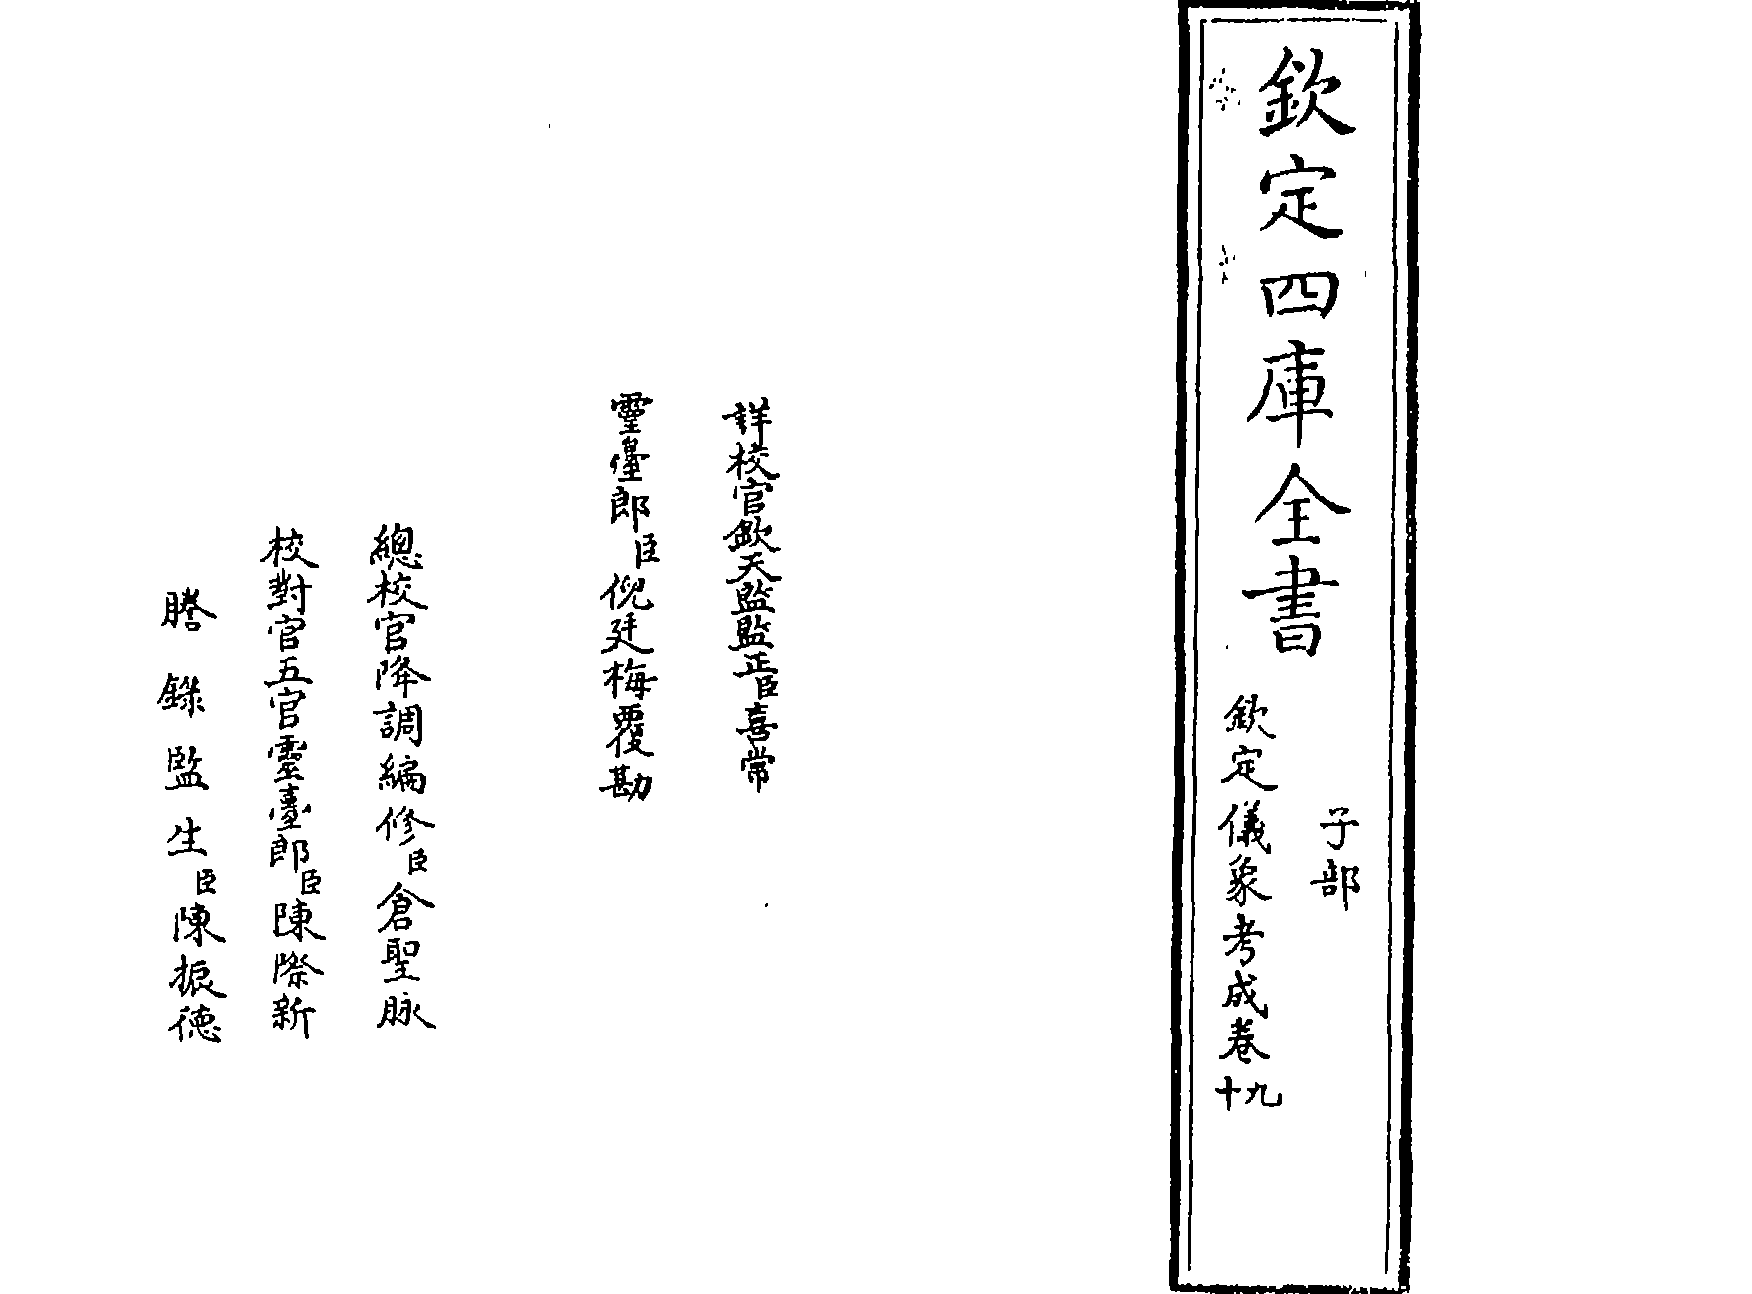
\includegraphics[width=\paperwidth,height=\paperheight,keepaspectratio]{img/0804.png}\clearpage
\begin{正文}
% ---- 册793 葉805 ----
\SetPageNumber{1}
欽定四庫全書\换行
欽定儀象考成卷九\换行
　恒星黄道經緯度表八\换行
　　黄道鶉火宫\双列{\右小列{赤道度附}\左小列{}}\换行
\char"200B\relax\换行
\char"200B\relax\换行
\char"200B\relax\换行
\char"200B\relax\换行
\char"200B\relax\换行
\char"200B\relax\换行
\char"200B\relax\换行
\char"200B\relax\换行
\char"200B\relax\换行
\char"200B\relax\换行
\char"200B\relax\换行
\char"200B\relax
\par
\end{正文}\clearpage
\嵌图{142.64pt}{201.94pt}{846.47pt}{585.91pt}{img/0808.png}
\begin{正文}
% ---- 册793 葉808 图版 ----
\SetPageNumber{2}
\插图页
\char"200B\relax\换行
\char"200B\relax\换行
\char"200B\relax\换行
\char"200B\relax\换行
\char"200B\relax\换行
\char"200B\relax\换行
\char"200B\relax\换行
\char"200B\relax\换行
\char"200B\relax\换行
\char"200B\relax\换行
\char"200B\relax\换行
\char"200B\relax\换行
\char"200B\relax\换行
\char"200B\relax\换行
\char"200B\relax\换行
\char"200B\relax
\恢复丝栏\par
\end{正文}\clearpage
\嵌图{144.63pt}{201.45pt}{842.50pt}{586.89pt}{img/0809.png}
\begin{正文}
% ---- 册793 葉809 图版 ----
\SetPageNumber{3}
\插图页
\char"200B\relax\换行
\char"200B\relax\换行
\char"200B\relax\换行
\char"200B\relax\换行
\char"200B\relax\换行
\char"200B\relax\换行
\char"200B\relax\换行
\char"200B\relax\换行
\char"200B\relax\换行
\char"200B\relax\换行
\char"200B\relax\换行
\char"200B\relax\换行
\char"200B\relax\换行
\char"200B\relax\换行
\char"200B\relax\换行
\char"200B\relax
\恢复丝栏\par
\end{正文}\clearpage
\嵌图{142.64pt}{201.00pt}{846.47pt}{587.79pt}{img/0812.png}
\begin{正文}
% ---- 册793 葉812 图版 ----
\SetPageNumber{4}
\插图页
\char"200B\relax\换行
\char"200B\relax\换行
\char"200B\relax\换行
\char"200B\relax\换行
\char"200B\relax\换行
\char"200B\relax\换行
\char"200B\relax\换行
\char"200B\relax\换行
\char"200B\relax\换行
\char"200B\relax\换行
\char"200B\relax\换行
\char"200B\relax\换行
\char"200B\relax\换行
\char"200B\relax\换行
\char"200B\relax\换行
\char"200B\relax
\恢复丝栏\par
\end{正文}\clearpage
\嵌图{148.61pt}{202.84pt}{834.55pt}{584.11pt}{img/0813.png}
\begin{正文}
% ---- 册793 葉813 图版 ----
\SetPageNumber{5}
\插图页
\char"200B\relax\换行
\char"200B\relax\换行
\char"200B\relax\换行
\char"200B\relax\换行
\char"200B\relax\换行
\char"200B\relax\换行
\char"200B\relax\换行
\char"200B\relax\换行
\char"200B\relax\换行
\char"200B\relax\换行
\char"200B\relax\换行
\char"200B\relax\换行
\char"200B\relax\换行
\char"200B\relax\换行
\char"200B\relax\换行
\char"200B\relax
\恢复丝栏\par
\end{正文}\clearpage
\嵌图{144.72pt}{202.49pt}{842.31pt}{584.82pt}{img/0816.png}
\begin{正文}
% ---- 册793 葉816 图版 ----
\SetPageNumber{6}
\插图页
\char"200B\relax\换行
\char"200B\relax\换行
\char"200B\relax\换行
\char"200B\relax\换行
\char"200B\relax\换行
\char"200B\relax\换行
\char"200B\relax\换行
\char"200B\relax\换行
\char"200B\relax\换行
\char"200B\relax\换行
\char"200B\relax\换行
\char"200B\relax\换行
\char"200B\relax\换行
\char"200B\relax\换行
\char"200B\relax\换行
\char"200B\relax
\恢复丝栏\par
\end{正文}\clearpage
\嵌图{144.72pt}{201.04pt}{842.31pt}{587.70pt}{img/0817.png}
\begin{正文}
% ---- 册793 葉817 图版 ----
\SetPageNumber{7}
\插图页
\char"200B\relax\换行
\char"200B\relax\换行
\char"200B\relax\换行
\char"200B\relax\换行
\char"200B\relax\换行
\char"200B\relax\换行
\char"200B\relax\换行
\char"200B\relax\换行
\char"200B\relax\换行
\char"200B\relax\换行
\char"200B\relax\换行
\char"200B\relax\换行
\char"200B\relax\换行
\char"200B\relax\换行
\char"200B\relax\换行
\char"200B\relax
\恢复丝栏\par
\end{正文}\clearpage
\嵌图{144.63pt}{200.98pt}{842.50pt}{587.83pt}{img/0820.png}
\begin{正文}
% ---- 册793 葉820 图版 ----
\SetPageNumber{8}
\插图页
\char"200B\relax\换行
\char"200B\relax\换行
\char"200B\relax\换行
\char"200B\relax\换行
\char"200B\relax\换行
\char"200B\relax\换行
\char"200B\relax\换行
\char"200B\relax\换行
\char"200B\relax\换行
\char"200B\relax\换行
\char"200B\relax\换行
\char"200B\relax\换行
\char"200B\relax\换行
\char"200B\relax\换行
\char"200B\relax\换行
\char"200B\relax
\恢复丝栏\par
\end{正文}\clearpage
\嵌图{144.63pt}{200.96pt}{842.50pt}{587.87pt}{img/0821.png}
\begin{正文}
% ---- 册793 葉821 图版 ----
\SetPageNumber{9}
\插图页
\char"200B\relax\换行
\char"200B\relax\换行
\char"200B\relax\换行
\char"200B\relax\换行
\char"200B\relax\换行
\char"200B\relax\换行
\char"200B\relax\换行
\char"200B\relax\换行
\char"200B\relax\换行
\char"200B\relax\换行
\char"200B\relax\换行
\char"200B\relax\换行
\char"200B\relax\换行
\char"200B\relax\换行
\char"200B\relax\换行
\char"200B\relax
\恢复丝栏\par
\end{正文}\clearpage
\嵌图{144.68pt}{202.94pt}{842.41pt}{583.90pt}{img/0824.png}
\begin{正文}
% ---- 册793 葉824 图版 ----
\SetPageNumber{10}
\插图页
\char"200B\relax\换行
\char"200B\relax\换行
\char"200B\relax\换行
\char"200B\relax\换行
\char"200B\relax\换行
\char"200B\relax\换行
\char"200B\relax\换行
\char"200B\relax\换行
\char"200B\relax\换行
\char"200B\relax\换行
\char"200B\relax\换行
\char"200B\relax\换行
\char"200B\relax\换行
\char"200B\relax\换行
\char"200B\relax\换行
\char"200B\relax
\恢复丝栏\par
\end{正文}\clearpage
\嵌图{144.68pt}{201.98pt}{842.41pt}{585.83pt}{img/0825.png}
\begin{正文}
% ---- 册793 葉825 图版 ----
\SetPageNumber{11}
\插图页
\char"200B\relax\换行
\char"200B\relax\换行
\char"200B\relax\换行
\char"200B\relax\换行
\char"200B\relax\换行
\char"200B\relax\换行
\char"200B\relax\换行
\char"200B\relax\换行
\char"200B\relax\换行
\char"200B\relax\换行
\char"200B\relax\换行
\char"200B\relax\换行
\char"200B\relax\换行
\char"200B\relax\换行
\char"200B\relax\换行
\char"200B\relax
\恢复丝栏\par
\end{正文}\clearpage
\嵌图{144.68pt}{202.94pt}{842.41pt}{583.92pt}{img/0828.png}
\begin{正文}
% ---- 册793 葉828 图版 ----
\SetPageNumber{12}
\插图页
\char"200B\relax\换行
\char"200B\relax\换行
\char"200B\relax\换行
\char"200B\relax\换行
\char"200B\relax\换行
\char"200B\relax\换行
\char"200B\relax\换行
\char"200B\relax\换行
\char"200B\relax\换行
\char"200B\relax\换行
\char"200B\relax\换行
\char"200B\relax\换行
\char"200B\relax\换行
\char"200B\relax\换行
\char"200B\relax\换行
\char"200B\relax
\恢复丝栏\par
\end{正文}\clearpage
\嵌图{144.68pt}{200.04pt}{842.41pt}{589.71pt}{img/0829.png}
\begin{正文}
% ---- 册793 葉829 图版 ----
\SetPageNumber{13}
\插图页
\char"200B\relax\换行
\char"200B\relax\换行
\char"200B\relax\换行
\char"200B\relax\换行
\char"200B\relax\换行
\char"200B\relax\换行
\char"200B\relax\换行
\char"200B\relax\换行
\char"200B\relax\换行
\char"200B\relax\换行
\char"200B\relax\换行
\char"200B\relax\换行
\char"200B\relax\换行
\char"200B\relax\换行
\char"200B\relax\换行
\char"200B\relax
\恢复丝栏\par
\end{正文}\clearpage
\嵌图{144.63pt}{202.94pt}{842.50pt}{583.92pt}{img/0832.png}
\begin{正文}
% ---- 册793 葉832 图版 ----
\SetPageNumber{14}
\插图页
\char"200B\relax\换行
\char"200B\relax\换行
\char"200B\relax\换行
\char"200B\relax\换行
\char"200B\relax\换行
\char"200B\relax\换行
\char"200B\relax\换行
\char"200B\relax\换行
\char"200B\relax\换行
\char"200B\relax\换行
\char"200B\relax\换行
\char"200B\relax\换行
\char"200B\relax\换行
\char"200B\relax\换行
\char"200B\relax\换行
\char"200B\relax
\恢复丝栏\par
\end{正文}\clearpage
\嵌图{144.63pt}{200.51pt}{842.50pt}{588.76pt}{img/0833.png}
\begin{正文}
% ---- 册793 葉833 图版 ----
\SetPageNumber{15}
\插图页
\char"200B\relax\换行
\char"200B\relax\换行
\char"200B\relax\换行
\char"200B\relax\换行
\char"200B\relax\换行
\char"200B\relax\换行
\char"200B\relax\换行
\char"200B\relax\换行
\char"200B\relax\换行
\char"200B\relax\换行
\char"200B\relax\换行
\char"200B\relax\换行
\char"200B\relax\换行
\char"200B\relax\换行
\char"200B\relax\换行
\char"200B\relax
\恢复丝栏\par
\end{正文}\clearpage
\嵌图{144.63pt}{201.51pt}{842.50pt}{586.77pt}{img/0836.png}
\begin{正文}
% ---- 册793 葉836 图版 ----
\SetPageNumber{16}
\插图页
\char"200B\relax\换行
\char"200B\relax\换行
\char"200B\relax\换行
\char"200B\relax\换行
\char"200B\relax\换行
\char"200B\relax\换行
\char"200B\relax\换行
\char"200B\relax\换行
\char"200B\relax\换行
\char"200B\relax\换行
\char"200B\relax\换行
\char"200B\relax\换行
\char"200B\relax\换行
\char"200B\relax\换行
\char"200B\relax\换行
\char"200B\relax
\恢复丝栏\par
\end{正文}\clearpage
\嵌图{146.62pt}{201.91pt}{838.53pt}{585.98pt}{img/0837.png}
\begin{正文}
% ---- 册793 葉837 图版 ----
\SetPageNumber{17}
\插图页
\char"200B\relax\换行
\char"200B\relax\换行
\char"200B\relax\换行
\char"200B\relax\换行
\char"200B\relax\换行
\char"200B\relax\换行
\char"200B\relax\换行
\char"200B\relax\换行
\char"200B\relax\换行
\char"200B\relax\换行
\char"200B\relax\换行
\char"200B\relax\换行
\char"200B\relax\换行
\char"200B\relax\换行
\char"200B\relax\换行
\char"200B\relax
\恢复丝栏\par
\end{正文}\clearpage
\嵌图{142.64pt}{201.50pt}{846.47pt}{586.78pt}{img/0840.png}
\begin{正文}
% ---- 册793 葉840 图版 ----
\SetPageNumber{18}
\插图页
\char"200B\relax\换行
\char"200B\relax\换行
\char"200B\relax\换行
\char"200B\relax\换行
\char"200B\relax\换行
\char"200B\relax\换行
\char"200B\relax\换行
\char"200B\relax\换行
\char"200B\relax\换行
\char"200B\relax\换行
\char"200B\relax\换行
\char"200B\relax\换行
\char"200B\relax\换行
\char"200B\relax\换行
\char"200B\relax\换行
\char"200B\relax
\恢复丝栏\par
\end{正文}\clearpage
\嵌图{142.64pt}{201.01pt}{846.47pt}{587.77pt}{img/0841.png}
\begin{正文}
% ---- 册793 葉841 图版 ----
\SetPageNumber{19}
\插图页
\char"200B\relax\换行
\char"200B\relax\换行
\char"200B\relax\换行
\char"200B\relax\换行
\char"200B\relax\换行
\char"200B\relax\换行
\char"200B\relax\换行
\char"200B\relax\换行
\char"200B\relax\换行
\char"200B\relax\换行
\char"200B\relax\换行
\char"200B\relax\换行
\char"200B\relax\换行
\char"200B\relax\换行
\char"200B\relax\换行
\char"200B\relax
\恢复丝栏\par
\end{正文}\clearpage
\嵌图{146.62pt}{200.02pt}{838.53pt}{589.74pt}{img/0844.png}
\begin{正文}
% ---- 册793 葉844 图版 ----
\SetPageNumber{20}
\插图页
\char"200B\relax\换行
\char"200B\relax\换行
\char"200B\relax\换行
\char"200B\relax\换行
\char"200B\relax\换行
\char"200B\relax\换行
\char"200B\relax\换行
\char"200B\relax\换行
\char"200B\relax\换行
\char"200B\relax\换行
\char"200B\relax\换行
\char"200B\relax\换行
\char"200B\relax\换行
\char"200B\relax\换行
\char"200B\relax\换行
\char"200B\relax
\恢复丝栏\par
\end{正文}\clearpage
\嵌图{142.64pt}{202.82pt}{846.47pt}{584.14pt}{img/0845.png}
\begin{正文}
% ---- 册793 葉845 图版 ----
\SetPageNumber{21}
\插图页
\char"200B\relax\换行
\char"200B\relax\换行
\char"200B\relax\换行
\char"200B\relax\换行
\char"200B\relax\换行
\char"200B\relax\换行
\char"200B\relax\换行
\char"200B\relax\换行
\char"200B\relax\换行
\char"200B\relax\换行
\char"200B\relax\换行
\char"200B\relax\换行
\char"200B\relax\换行
\char"200B\relax\换行
\char"200B\relax\换行
\char"200B\relax
\恢复丝栏\par
\end{正文}\clearpage
\嵌图{146.62pt}{201.02pt}{838.53pt}{587.76pt}{img/0848.png}
\begin{正文}
% ---- 册793 葉848 图版 ----
\SetPageNumber{22}
\插图页
\char"200B\relax\换行
\char"200B\relax\换行
\char"200B\relax\换行
\char"200B\relax\换行
\char"200B\relax\换行
\char"200B\relax\换行
\char"200B\relax\换行
\char"200B\relax\换行
\char"200B\relax\换行
\char"200B\relax\换行
\char"200B\relax\换行
\char"200B\relax\换行
\char"200B\relax\换行
\char"200B\relax\换行
\char"200B\relax\换行
\char"200B\relax
\恢复丝栏\par
\end{正文}\clearpage
\嵌图{142.64pt}{199.59pt}{846.47pt}{590.61pt}{img/0849.png}
\begin{正文}
% ---- 册793 葉849 图版 ----
\SetPageNumber{23}
\插图页
\char"200B\relax\换行
\char"200B\relax\换行
\char"200B\relax\换行
\char"200B\relax\换行
\char"200B\relax\换行
\char"200B\relax\换行
\char"200B\relax\换行
\char"200B\relax\换行
\char"200B\relax\换行
\char"200B\relax\换行
\char"200B\relax\换行
\char"200B\relax\换行
\char"200B\relax\换行
\char"200B\relax\换行
\char"200B\relax\换行
\char"200B\relax
\恢复丝栏\par
\end{正文}\clearpage
\嵌图{150.30pt}{198.15pt}{831.15pt}{593.49pt}{img/0852.png}
\begin{正文}
% ---- 册793 葉852 图版 ----
\SetPageNumber{24}
\插图页
\char"200B\relax\换行
\char"200B\relax\换行
\char"200B\relax\换行
\char"200B\relax\换行
\char"200B\relax\换行
\char"200B\relax\换行
\char"200B\relax\换行
\char"200B\relax\换行
\char"200B\relax\换行
\char"200B\relax\换行
\char"200B\relax\换行
\char"200B\relax\换行
\char"200B\relax\换行
\char"200B\relax\换行
\char"200B\relax\换行
\char"200B\relax
\恢复丝栏\par
\end{正文}\clearpage
\嵌图{150.93pt}{209.28pt}{397.09pt}{583.55pt}{img/0853.png}
\begin{正文}
% ---- 册793 葉853 ----
\SetPageNumber{25}
\插图页
\char"200B\relax\换行
\char"200B\relax\换行
\char"200B\relax\换行
\char"200B\relax\换行
\char"200B\relax\换行
\char"200B\relax\换行
\char"200B\relax\换行
\char"200B\relax\换行
\恢复丝栏
\char"200B\relax\换行
\char"200B\relax\换行
\char"200B\relax\换行
\char"200B\relax\换行
\char"200B\relax\换行
\char"200B\relax\换行
\char"200B\relax\换行
欽定儀象考成卷九
\par

% ======== 卷十（8行21字）========
\par\end{正文}\clearpage
\chapter*{欽定儀象考成卷十}
\begin{正文}
% ---- 册793 葉856 ----
\SetPageNumber{1}
欽定四庫全書\换行
欽定儀象考成卷十\换行
　恒星黄道經緯度表九\换行
　　黄道鶉尾宫\双列{\右小列{赤道度附}\左小列{}}\换行
\char"200B\relax\换行
\char"200B\relax\换行
\char"200B\relax\换行
\char"200B\relax\换行
\char"200B\relax\换行
\char"200B\relax\换行
\char"200B\relax\换行
\char"200B\relax\换行
\char"200B\relax\换行
\char"200B\relax\换行
\char"200B\relax\换行
\char"200B\relax
\par
\end{正文}\clearpage
\嵌图{144.63pt}{201.50pt}{842.50pt}{586.80pt}{img/0857.png}
\begin{正文}
% ---- 册793 葉857 图版 ----
\SetPageNumber{2}
\插图页
\char"200B\relax\换行
\char"200B\relax\换行
\char"200B\relax\换行
\char"200B\relax\换行
\char"200B\relax\换行
\char"200B\relax\换行
\char"200B\relax\换行
\char"200B\relax\换行
\char"200B\relax\换行
\char"200B\relax\换行
\char"200B\relax\换行
\char"200B\relax\换行
\char"200B\relax\换行
\char"200B\relax\换行
\char"200B\relax\换行
\char"200B\relax
\恢复丝栏\par
\end{正文}\clearpage
\嵌图{144.63pt}{201.53pt}{842.50pt}{586.74pt}{img/0860.png}
\begin{正文}
% ---- 册793 葉860 图版 ----
\SetPageNumber{3}
\插图页
\char"200B\relax\换行
\char"200B\relax\换行
\char"200B\relax\换行
\char"200B\relax\换行
\char"200B\relax\换行
\char"200B\relax\换行
\char"200B\relax\换行
\char"200B\relax\换行
\char"200B\relax\换行
\char"200B\relax\换行
\char"200B\relax\换行
\char"200B\relax\换行
\char"200B\relax\换行
\char"200B\relax\换行
\char"200B\relax\换行
\char"200B\relax
\恢复丝栏\par
\end{正文}\clearpage
\嵌图{146.62pt}{201.46pt}{838.53pt}{586.87pt}{img/0861.png}
\begin{正文}
% ---- 册793 葉861 图版 ----
\SetPageNumber{4}
\插图页
\char"200B\relax\换行
\char"200B\relax\换行
\char"200B\relax\换行
\char"200B\relax\换行
\char"200B\relax\换行
\char"200B\relax\换行
\char"200B\relax\换行
\char"200B\relax\换行
\char"200B\relax\换行
\char"200B\relax\换行
\char"200B\relax\换行
\char"200B\relax\换行
\char"200B\relax\换行
\char"200B\relax\换行
\char"200B\relax\换行
\char"200B\relax
\恢复丝栏\par
\end{正文}\clearpage
\嵌图{146.56pt}{201.05pt}{838.64pt}{587.69pt}{img/0864.png}
\begin{正文}
% ---- 册793 葉864 图版 ----
\SetPageNumber{5}
\插图页
\char"200B\relax\换行
\char"200B\relax\换行
\char"200B\relax\换行
\char"200B\relax\换行
\char"200B\relax\换行
\char"200B\relax\换行
\char"200B\relax\换行
\char"200B\relax\换行
\char"200B\relax\换行
\char"200B\relax\换行
\char"200B\relax\换行
\char"200B\relax\换行
\char"200B\relax\换行
\char"200B\relax\换行
\char"200B\relax\换行
\char"200B\relax
\恢复丝栏\par
\end{正文}\clearpage
\嵌图{146.56pt}{201.50pt}{838.64pt}{586.78pt}{img/0865.png}
\begin{正文}
% ---- 册793 葉865 图版 ----
\SetPageNumber{6}
\插图页
\char"200B\relax\换行
\char"200B\relax\换行
\char"200B\relax\换行
\char"200B\relax\换行
\char"200B\relax\换行
\char"200B\relax\换行
\char"200B\relax\换行
\char"200B\relax\换行
\char"200B\relax\换行
\char"200B\relax\换行
\char"200B\relax\换行
\char"200B\relax\换行
\char"200B\relax\换行
\char"200B\relax\换行
\char"200B\relax\换行
\char"200B\relax
\恢复丝栏\par
\end{正文}\clearpage
\嵌图{144.63pt}{200.09pt}{842.50pt}{589.60pt}{img/0868.png}
\begin{正文}
% ---- 册793 葉868 图版 ----
\SetPageNumber{7}
\插图页
\char"200B\relax\换行
\char"200B\relax\换行
\char"200B\relax\换行
\char"200B\relax\换行
\char"200B\relax\换行
\char"200B\relax\换行
\char"200B\relax\换行
\char"200B\relax\换行
\char"200B\relax\换行
\char"200B\relax\换行
\char"200B\relax\换行
\char"200B\relax\换行
\char"200B\relax\换行
\char"200B\relax\换行
\char"200B\relax\换行
\char"200B\relax
\恢复丝栏\par
\end{正文}\clearpage
\嵌图{146.62pt}{200.51pt}{838.53pt}{588.76pt}{img/0869.png}
\begin{正文}
% ---- 册793 葉869 图版 ----
\SetPageNumber{8}
\插图页
\char"200B\relax\换行
\char"200B\relax\换行
\char"200B\relax\换行
\char"200B\relax\换行
\char"200B\relax\换行
\char"200B\relax\换行
\char"200B\relax\换行
\char"200B\relax\换行
\char"200B\relax\换行
\char"200B\relax\换行
\char"200B\relax\换行
\char"200B\relax\换行
\char"200B\relax\换行
\char"200B\relax\换行
\char"200B\relax\换行
\char"200B\relax
\恢复丝栏\par
\end{正文}\clearpage
\嵌图{144.63pt}{199.14pt}{842.50pt}{591.50pt}{img/0872.png}
\begin{正文}
% ---- 册793 葉872 图版 ----
\SetPageNumber{9}
\插图页
\char"200B\relax\换行
\char"200B\relax\换行
\char"200B\relax\换行
\char"200B\relax\换行
\char"200B\relax\换行
\char"200B\relax\换行
\char"200B\relax\换行
\char"200B\relax\换行
\char"200B\relax\换行
\char"200B\relax\换行
\char"200B\relax\换行
\char"200B\relax\换行
\char"200B\relax\换行
\char"200B\relax\换行
\char"200B\relax\换行
\char"200B\relax
\恢复丝栏\par
\end{正文}\clearpage
\嵌图{146.62pt}{201.49pt}{838.53pt}{586.81pt}{img/0873.png}
\begin{正文}
% ---- 册793 葉873 图版 ----
\SetPageNumber{10}
\插图页
\char"200B\relax\换行
\char"200B\relax\换行
\char"200B\relax\换行
\char"200B\relax\换行
\char"200B\relax\换行
\char"200B\relax\换行
\char"200B\relax\换行
\char"200B\relax\换行
\char"200B\relax\换行
\char"200B\relax\换行
\char"200B\relax\换行
\char"200B\relax\换行
\char"200B\relax\换行
\char"200B\relax\换行
\char"200B\relax\换行
\char"200B\relax
\恢复丝栏\par
\end{正文}\clearpage
\嵌图{144.63pt}{200.51pt}{842.50pt}{588.77pt}{img/0876.png}
\begin{正文}
% ---- 册793 葉876 图版 ----
\SetPageNumber{11}
\插图页
\char"200B\relax\换行
\char"200B\relax\换行
\char"200B\relax\换行
\char"200B\relax\换行
\char"200B\relax\换行
\char"200B\relax\换行
\char"200B\relax\换行
\char"200B\relax\换行
\char"200B\relax\换行
\char"200B\relax\换行
\char"200B\relax\换行
\char"200B\relax\换行
\char"200B\relax\换行
\char"200B\relax\换行
\char"200B\relax\换行
\char"200B\relax
\恢复丝栏\par
\end{正文}\clearpage
\嵌图{146.62pt}{199.08pt}{838.53pt}{591.64pt}{img/0877.png}
\begin{正文}
% ---- 册793 葉877 图版 ----
\SetPageNumber{12}
\插图页
\char"200B\relax\换行
\char"200B\relax\换行
\char"200B\relax\换行
\char"200B\relax\换行
\char"200B\relax\换行
\char"200B\relax\换行
\char"200B\relax\换行
\char"200B\relax\换行
\char"200B\relax\换行
\char"200B\relax\换行
\char"200B\relax\换行
\char"200B\relax\换行
\char"200B\relax\换行
\char"200B\relax\换行
\char"200B\relax\换行
\char"200B\relax
\恢复丝栏\par
\end{正文}\clearpage
\嵌图{142.68pt}{201.00pt}{846.40pt}{587.79pt}{img/0880.png}
\begin{正文}
% ---- 册793 葉880 图版 ----
\SetPageNumber{13}
\插图页
\char"200B\relax\换行
\char"200B\relax\换行
\char"200B\relax\换行
\char"200B\relax\换行
\char"200B\relax\换行
\char"200B\relax\换行
\char"200B\relax\换行
\char"200B\relax\换行
\char"200B\relax\换行
\char"200B\relax\换行
\char"200B\relax\换行
\char"200B\relax\换行
\char"200B\relax\换行
\char"200B\relax\换行
\char"200B\relax\换行
\char"200B\relax
\恢复丝栏\par
\end{正文}\clearpage
\嵌图{142.68pt}{201.96pt}{846.40pt}{585.86pt}{img/0881.png}
\begin{正文}
% ---- 册793 葉881 图版 ----
\SetPageNumber{14}
\插图页
\char"200B\relax\换行
\char"200B\relax\换行
\char"200B\relax\换行
\char"200B\relax\换行
\char"200B\relax\换行
\char"200B\relax\换行
\char"200B\relax\换行
\char"200B\relax\换行
\char"200B\relax\换行
\char"200B\relax\换行
\char"200B\relax\换行
\char"200B\relax\换行
\char"200B\relax\换行
\char"200B\relax\换行
\char"200B\relax\换行
\char"200B\relax
\恢复丝栏\par
\end{正文}\clearpage
\嵌图{144.63pt}{200.51pt}{842.50pt}{588.76pt}{img/0884.png}
\begin{正文}
% ---- 册793 葉884 图版 ----
\SetPageNumber{15}
\插图页
\char"200B\relax\换行
\char"200B\relax\换行
\char"200B\relax\换行
\char"200B\relax\换行
\char"200B\relax\换行
\char"200B\relax\换行
\char"200B\relax\换行
\char"200B\relax\换行
\char"200B\relax\换行
\char"200B\relax\换行
\char"200B\relax\换行
\char"200B\relax\换行
\char"200B\relax\换行
\char"200B\relax\换行
\char"200B\relax\换行
\char"200B\relax
\恢复丝栏\par
\end{正文}\clearpage
\嵌图{146.62pt}{201.91pt}{838.53pt}{585.98pt}{img/0885.png}
\begin{正文}
% ---- 册793 葉885 图版 ----
\SetPageNumber{16}
\插图页
\char"200B\relax\换行
\char"200B\relax\换行
\char"200B\relax\换行
\char"200B\relax\换行
\char"200B\relax\换行
\char"200B\relax\换行
\char"200B\relax\换行
\char"200B\relax\换行
\char"200B\relax\换行
\char"200B\relax\换行
\char"200B\relax\换行
\char"200B\relax\换行
\char"200B\relax\换行
\char"200B\relax\换行
\char"200B\relax\换行
\char"200B\relax
\恢复丝栏\par
\end{正文}\clearpage
\嵌图{144.63pt}{200.54pt}{842.50pt}{588.71pt}{img/0888.png}
\begin{正文}
% ---- 册793 葉888 图版 ----
\SetPageNumber{17}
\插图页
\char"200B\relax\换行
\char"200B\relax\换行
\char"200B\relax\换行
\char"200B\relax\换行
\char"200B\relax\换行
\char"200B\relax\换行
\char"200B\relax\换行
\char"200B\relax\换行
\char"200B\relax\换行
\char"200B\relax\换行
\char"200B\relax\换行
\char"200B\relax\换行
\char"200B\relax\换行
\char"200B\relax\换行
\char"200B\relax\换行
\char"200B\relax
\恢复丝栏\par
\end{正文}\clearpage
\嵌图{144.63pt}{198.65pt}{842.50pt}{592.48pt}{img/0889.png}
\begin{正文}
% ---- 册793 葉889 图版 ----
\SetPageNumber{18}
\插图页
\char"200B\relax\换行
\char"200B\relax\换行
\char"200B\relax\换行
\char"200B\relax\换行
\char"200B\relax\换行
\char"200B\relax\换行
\char"200B\relax\换行
\char"200B\relax\换行
\char"200B\relax\换行
\char"200B\relax\换行
\char"200B\relax\换行
\char"200B\relax\换行
\char"200B\relax\换行
\char"200B\relax\换行
\char"200B\relax\换行
\char"200B\relax
\恢复丝栏\par
\end{正文}\clearpage
\嵌图{145.26pt}{209.32pt}{402.76pt}{583.51pt}{img/0892.png}
\begin{正文}
% ---- 册793 葉892 ----
\SetPageNumber{19}
\插图页
\char"200B\relax\换行
\char"200B\relax\换行
\char"200B\relax\换行
\char"200B\relax\换行
\char"200B\relax\换行
\char"200B\relax\换行
\char"200B\relax\换行
\char"200B\relax\换行
\恢复丝栏
\char"200B\relax\换行
\char"200B\relax\换行
\char"200B\relax\换行
\char"200B\relax\换行
\char"200B\relax\换行
\char"200B\relax\换行
欽定儀象考成卷十\换行
\char"200B\relax
\par

% ======== 卷十一（8行21字）========
\par\end{正文}\clearpage
\chapter*{欽定儀象考成卷十一}
\begin{正文}
\end{正文}\clearpage

  % ======== 卷十四（8行21字）========
\chapter*{欽定儀象考成卷十四}
\begin{正文}
\end{正文}\clearpage
\thispagestyle{empty}\noindent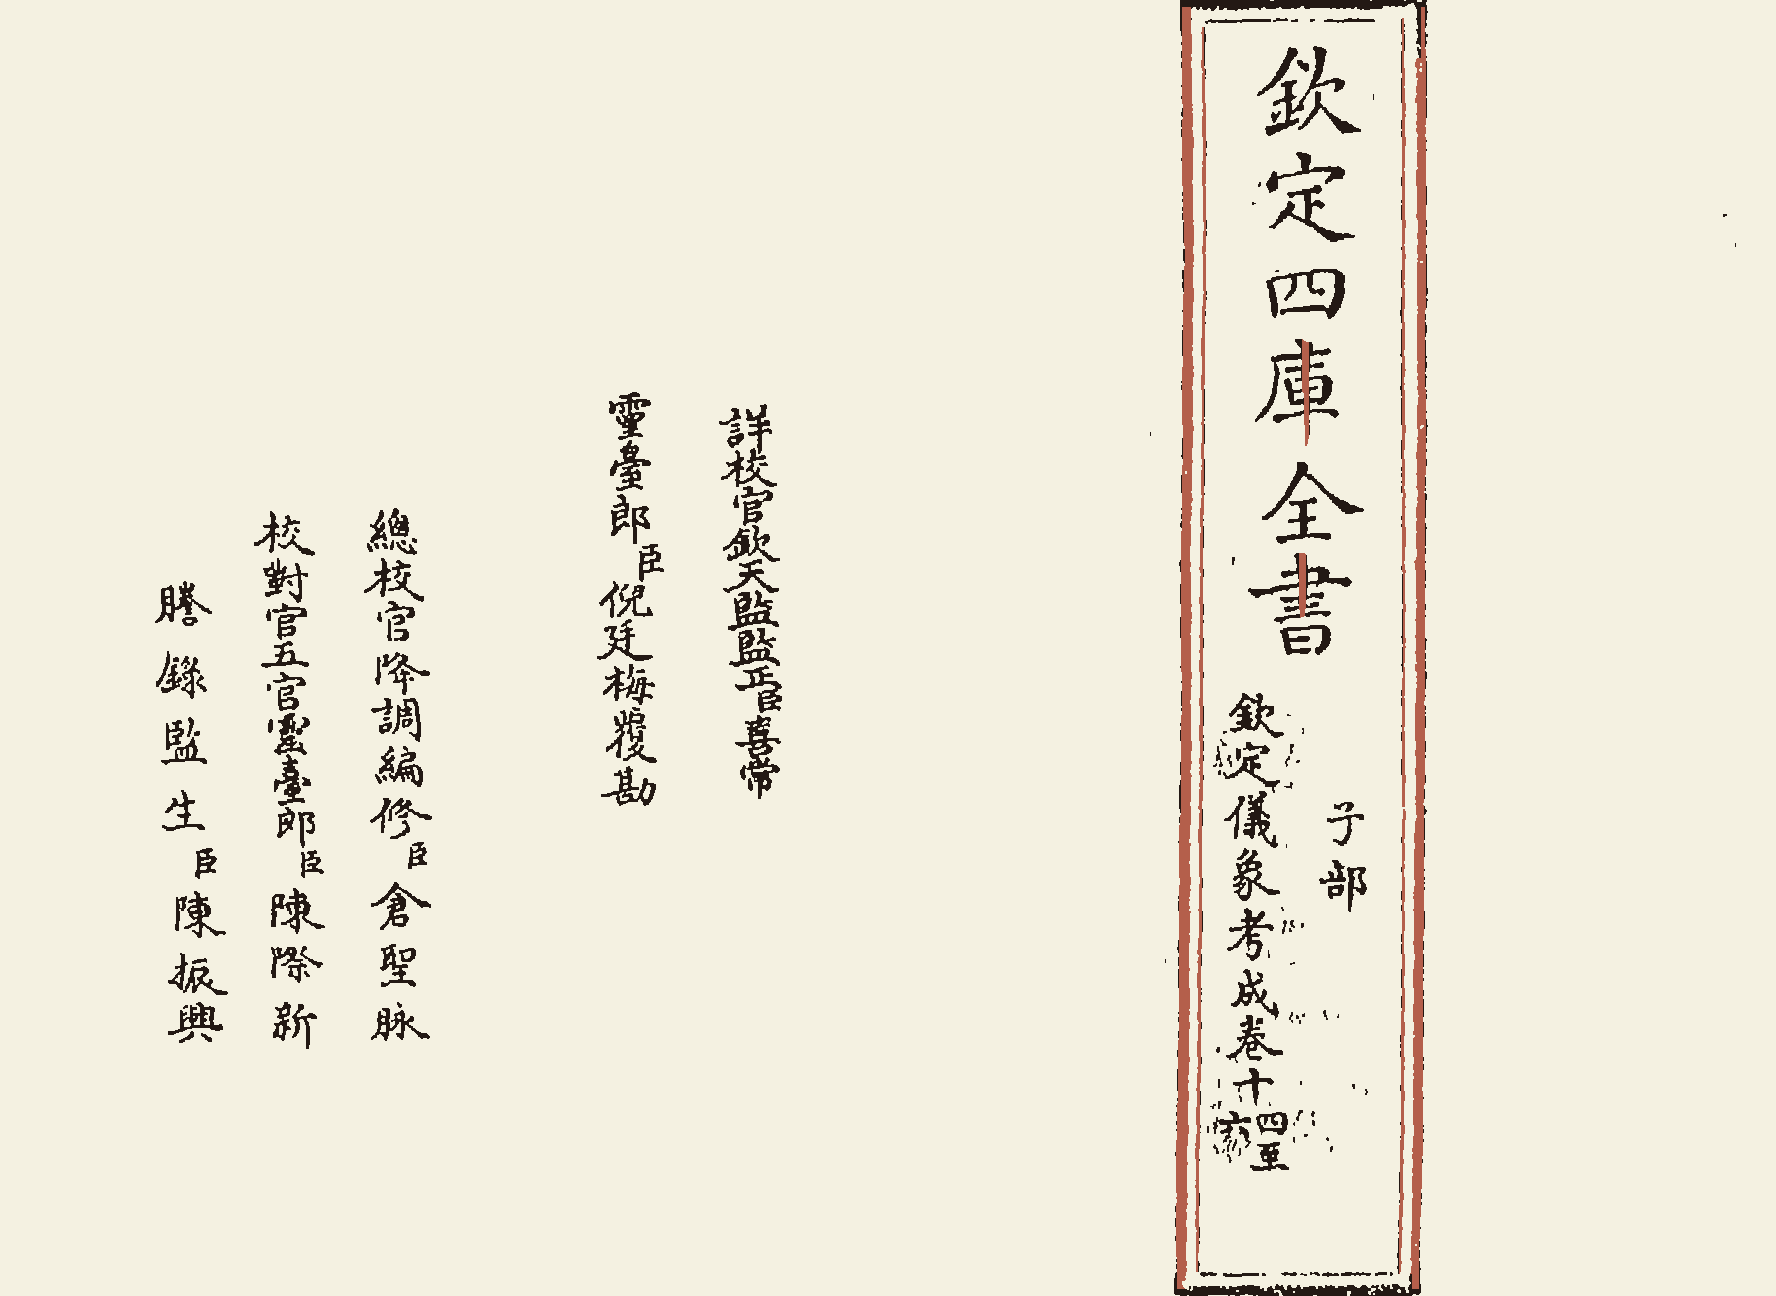
\includegraphics[width=\paperwidth,height=\paperheight,keepaspectratio]{img/1012.png}\clearpage
\begin{正文}
% ---- 册793 葉1013 ----
\SetPageNumber{1}
欽定四庫全書\换行
欽定儀象考成卷十四\换行
　恒星赤道經緯度表一\换行
　　赤道星紀宫\双列{\右小列{黄道度附}\左小列{}}\换行
\char"200B\relax\换行
\char"200B\relax\换行
\char"200B\relax\换行
\char"200B\relax\换行
\char"200B\relax\换行
\char"200B\relax\换行
\char"200B\relax\换行
\char"200B\relax\换行
\char"200B\relax\换行
\char"200B\relax\换行
\char"200B\relax\换行
\char"200B\relax
\par
\end{正文}\clearpage
\嵌图{142.64pt}{200.54pt}{846.47pt}{588.72pt}{img/1016.png}
\begin{正文}
% ---- 册793 葉1016 图版 ----
\SetPageNumber{2}
\插图页
\char"200B\relax\换行
\char"200B\relax\换行
\char"200B\relax\换行
\char"200B\relax\换行
\char"200B\relax\换行
\char"200B\relax\换行
\char"200B\relax\换行
\char"200B\relax\换行
\char"200B\relax\换行
\char"200B\relax\换行
\char"200B\relax\换行
\char"200B\relax\换行
\char"200B\relax\换行
\char"200B\relax\换行
\char"200B\relax\换行
\char"200B\relax
\恢复丝栏\par
\end{正文}\clearpage
\嵌图{148.61pt}{201.49pt}{834.55pt}{586.81pt}{img/1017.png}
\begin{正文}
% ---- 册793 葉1017 图版 ----
\SetPageNumber{3}
\插图页
\char"200B\relax\换行
\char"200B\relax\换行
\char"200B\relax\换行
\char"200B\relax\换行
\char"200B\relax\换行
\char"200B\relax\换行
\char"200B\relax\换行
\char"200B\relax\换行
\char"200B\relax\换行
\char"200B\relax\换行
\char"200B\relax\换行
\char"200B\relax\换行
\char"200B\relax\换行
\char"200B\relax\换行
\char"200B\relax\换行
\char"200B\relax
\恢复丝栏\par
\end{正文}\clearpage
\嵌图{142.72pt}{201.96pt}{846.33pt}{585.86pt}{img/1020.png}
\begin{正文}
% ---- 册793 葉1020 图版 ----
\SetPageNumber{4}
\插图页
\char"200B\relax\换行
\char"200B\relax\换行
\char"200B\relax\换行
\char"200B\relax\换行
\char"200B\relax\换行
\char"200B\relax\换行
\char"200B\relax\换行
\char"200B\relax\换行
\char"200B\relax\换行
\char"200B\relax\换行
\char"200B\relax\换行
\char"200B\relax\换行
\char"200B\relax\换行
\char"200B\relax\换行
\char"200B\relax\换行
\char"200B\relax
\恢复丝栏\par
\end{正文}\clearpage
\嵌图{144.72pt}{201.47pt}{842.31pt}{586.86pt}{img/1021.png}
\begin{正文}
% ---- 册793 葉1021 图版 ----
\SetPageNumber{5}
\插图页
\char"200B\relax\换行
\char"200B\relax\换行
\char"200B\relax\换行
\char"200B\relax\换行
\char"200B\relax\换行
\char"200B\relax\换行
\char"200B\relax\换行
\char"200B\relax\换行
\char"200B\relax\换行
\char"200B\relax\换行
\char"200B\relax\换行
\char"200B\relax\换行
\char"200B\relax\换行
\char"200B\relax\换行
\char"200B\relax\换行
\char"200B\relax
\恢复丝栏\par
\end{正文}\clearpage
\嵌图{144.63pt}{200.06pt}{842.50pt}{589.67pt}{img/1024.png}
\begin{正文}
% ---- 册793 葉1024 图版 ----
\SetPageNumber{6}
\插图页
\char"200B\relax\换行
\char"200B\relax\换行
\char"200B\relax\换行
\char"200B\relax\换行
\char"200B\relax\换行
\char"200B\relax\换行
\char"200B\relax\换行
\char"200B\relax\换行
\char"200B\relax\换行
\char"200B\relax\换行
\char"200B\relax\换行
\char"200B\relax\换行
\char"200B\relax\换行
\char"200B\relax\换行
\char"200B\relax\换行
\char"200B\relax
\恢复丝栏\par
\end{正文}\clearpage
\嵌图{144.63pt}{200.54pt}{842.50pt}{588.72pt}{img/1025.png}
\begin{正文}
% ---- 册793 葉1025 图版 ----
\SetPageNumber{7}
\插图页
\char"200B\relax\换行
\char"200B\relax\换行
\char"200B\relax\换行
\char"200B\relax\换行
\char"200B\relax\换行
\char"200B\relax\换行
\char"200B\relax\换行
\char"200B\relax\换行
\char"200B\relax\换行
\char"200B\relax\换行
\char"200B\relax\换行
\char"200B\relax\换行
\char"200B\relax\换行
\char"200B\relax\换行
\char"200B\relax\换行
\char"200B\relax
\恢复丝栏\par
\end{正文}\clearpage
\嵌图{142.72pt}{201.01pt}{846.33pt}{587.77pt}{img/1028.png}
\begin{正文}
% ---- 册793 葉1028 图版 ----
\SetPageNumber{8}
\插图页
\char"200B\relax\换行
\char"200B\relax\换行
\char"200B\relax\换行
\char"200B\relax\换行
\char"200B\relax\换行
\char"200B\relax\换行
\char"200B\relax\换行
\char"200B\relax\换行
\char"200B\relax\换行
\char"200B\relax\换行
\char"200B\relax\换行
\char"200B\relax\换行
\char"200B\relax\换行
\char"200B\relax\换行
\char"200B\relax\换行
\char"200B\relax
\恢复丝栏\par
\end{正文}\clearpage
\嵌图{144.72pt}{200.98pt}{842.31pt}{587.83pt}{img/1029.png}
\begin{正文}
% ---- 册793 葉1029 图版 ----
\SetPageNumber{9}
\插图页
\char"200B\relax\换行
\char"200B\relax\换行
\char"200B\relax\换行
\char"200B\relax\换行
\char"200B\relax\换行
\char"200B\relax\换行
\char"200B\relax\换行
\char"200B\relax\换行
\char"200B\relax\换行
\char"200B\relax\换行
\char"200B\relax\换行
\char"200B\relax\换行
\char"200B\relax\换行
\char"200B\relax\换行
\char"200B\relax\换行
\char"200B\relax
\恢复丝栏\par
\end{正文}\clearpage
\嵌图{142.64pt}{200.06pt}{846.47pt}{589.67pt}{img/1032.png}
\begin{正文}
% ---- 册793 葉1032 图版 ----
\SetPageNumber{10}
\插图页
\char"200B\relax\换行
\char"200B\relax\换行
\char"200B\relax\换行
\char"200B\relax\换行
\char"200B\relax\换行
\char"200B\relax\换行
\char"200B\relax\换行
\char"200B\relax\换行
\char"200B\relax\换行
\char"200B\relax\换行
\char"200B\relax\换行
\char"200B\relax\换行
\char"200B\relax\换行
\char"200B\relax\换行
\char"200B\relax\换行
\char"200B\relax
\恢复丝栏\par
\end{正文}\clearpage
\嵌图{144.63pt}{200.06pt}{842.50pt}{589.68pt}{img/1033.png}
\begin{正文}
% ---- 册793 葉1033 图版 ----
\SetPageNumber{11}
\插图页
\char"200B\relax\换行
\char"200B\relax\换行
\char"200B\relax\换行
\char"200B\relax\换行
\char"200B\relax\换行
\char"200B\relax\换行
\char"200B\relax\换行
\char"200B\relax\换行
\char"200B\relax\换行
\char"200B\relax\换行
\char"200B\relax\换行
\char"200B\relax\换行
\char"200B\relax\换行
\char"200B\relax\换行
\char"200B\relax\换行
\char"200B\relax
\恢复丝栏\par
\end{正文}\clearpage
\嵌图{146.62pt}{199.56pt}{838.53pt}{590.66pt}{img/1036.png}
\begin{正文}
% ---- 册793 葉1036 图版 ----
\SetPageNumber{12}
\插图页
\char"200B\relax\换行
\char"200B\relax\换行
\char"200B\relax\换行
\char"200B\relax\换行
\char"200B\relax\换行
\char"200B\relax\换行
\char"200B\relax\换行
\char"200B\relax\换行
\char"200B\relax\换行
\char"200B\relax\换行
\char"200B\relax\换行
\char"200B\relax\换行
\char"200B\relax\换行
\char"200B\relax\换行
\char"200B\relax\换行
\char"200B\relax
\恢复丝栏\par
\end{正文}\clearpage
\嵌图{144.63pt}{200.96pt}{842.50pt}{587.87pt}{img/1037.png}
\begin{正文}
% ---- 册793 葉1037 图版 ----
\SetPageNumber{13}
\插图页
\char"200B\relax\换行
\char"200B\relax\换行
\char"200B\relax\换行
\char"200B\relax\换行
\char"200B\relax\换行
\char"200B\relax\换行
\char"200B\relax\换行
\char"200B\relax\换行
\char"200B\relax\换行
\char"200B\relax\换行
\char"200B\relax\换行
\char"200B\relax\换行
\char"200B\relax\换行
\char"200B\relax\换行
\char"200B\relax\换行
\char"200B\relax
\恢复丝栏\par
\end{正文}\clearpage
\嵌图{142.68pt}{202.98pt}{846.40pt}{583.83pt}{img/1040.png}
\begin{正文}
% ---- 册793 葉1040 图版 ----
\SetPageNumber{14}
\插图页
\char"200B\relax\换行
\char"200B\relax\换行
\char"200B\relax\换行
\char"200B\relax\换行
\char"200B\relax\换行
\char"200B\relax\换行
\char"200B\relax\换行
\char"200B\relax\换行
\char"200B\relax\换行
\char"200B\relax\换行
\char"200B\relax\换行
\char"200B\relax\换行
\char"200B\relax\换行
\char"200B\relax\换行
\char"200B\relax\换行
\char"200B\relax
\恢复丝栏\par
\end{正文}\clearpage
\嵌图{144.68pt}{200.58pt}{842.41pt}{588.62pt}{img/1041.png}
\begin{正文}
% ---- 册793 葉1041 图版 ----
\SetPageNumber{15}
\插图页
\char"200B\relax\换行
\char"200B\relax\换行
\char"200B\relax\换行
\char"200B\relax\换行
\char"200B\relax\换行
\char"200B\relax\换行
\char"200B\relax\换行
\char"200B\relax\换行
\char"200B\relax\换行
\char"200B\relax\换行
\char"200B\relax\换行
\char"200B\relax\换行
\char"200B\relax\换行
\char"200B\relax\换行
\char"200B\relax\换行
\char"200B\relax
\恢复丝栏\par
\end{正文}\clearpage
\嵌图{146.62pt}{203.37pt}{838.53pt}{583.04pt}{img/1044.png}
\begin{正文}
% ---- 册793 葉1044 图版 ----
\SetPageNumber{16}
\插图页
\char"200B\relax\换行
\char"200B\relax\换行
\char"200B\relax\换行
\char"200B\relax\换行
\char"200B\relax\换行
\char"200B\relax\换行
\char"200B\relax\换行
\char"200B\relax\换行
\char"200B\relax\换行
\char"200B\relax\换行
\char"200B\relax\换行
\char"200B\relax\换行
\char"200B\relax\换行
\char"200B\relax\换行
\char"200B\relax\换行
\char"200B\relax
\恢复丝栏\par
\end{正文}\clearpage
\嵌图{142.64pt}{202.87pt}{846.47pt}{584.06pt}{img/1045.png}
\begin{正文}
% ---- 册793 葉1045 图版 ----
\SetPageNumber{17}
\插图页
\char"200B\relax\换行
\char"200B\relax\换行
\char"200B\relax\换行
\char"200B\relax\换行
\char"200B\relax\换行
\char"200B\relax\换行
\char"200B\relax\换行
\char"200B\relax\换行
\char"200B\relax\换行
\char"200B\relax\换行
\char"200B\relax\换行
\char"200B\relax\换行
\char"200B\relax\换行
\char"200B\relax\换行
\char"200B\relax\换行
\char"200B\relax
\恢复丝栏\par
\end{正文}\clearpage
\嵌图{144.72pt}{201.07pt}{842.31pt}{587.66pt}{img/1048.png}
\begin{正文}
% ---- 册793 葉1048 图版 ----
\SetPageNumber{18}
\插图页
\char"200B\relax\换行
\char"200B\relax\换行
\char"200B\relax\换行
\char"200B\relax\换行
\char"200B\relax\换行
\char"200B\relax\换行
\char"200B\relax\换行
\char"200B\relax\换行
\char"200B\relax\换行
\char"200B\relax\换行
\char"200B\relax\换行
\char"200B\relax\换行
\char"200B\relax\换行
\char"200B\relax\换行
\char"200B\relax\换行
\char"200B\relax
\恢复丝栏\par
\end{正文}\clearpage
\嵌图{142.72pt}{202.94pt}{846.33pt}{583.90pt}{img/1049.png}
\begin{正文}
% ---- 册793 葉1049 图版 ----
\SetPageNumber{19}
\插图页
\char"200B\relax\换行
\char"200B\relax\换行
\char"200B\relax\换行
\char"200B\relax\换行
\char"200B\relax\换行
\char"200B\relax\换行
\char"200B\relax\换行
\char"200B\relax\换行
\char"200B\relax\换行
\char"200B\relax\换行
\char"200B\relax\换行
\char"200B\relax\换行
\char"200B\relax\换行
\char"200B\relax\换行
\char"200B\relax\换行
\char"200B\relax
\恢复丝栏\par
\end{正文}\clearpage
\嵌图{142.72pt}{202.41pt}{846.33pt}{584.97pt}{img/1052.png}
\begin{正文}
% ---- 册793 葉1052 图版 ----
\SetPageNumber{20}
\插图页
\char"200B\relax\换行
\char"200B\relax\换行
\char"200B\relax\换行
\char"200B\relax\换行
\char"200B\relax\换行
\char"200B\relax\换行
\char"200B\relax\换行
\char"200B\relax\换行
\char"200B\relax\换行
\char"200B\relax\换行
\char"200B\relax\换行
\char"200B\relax\换行
\char"200B\relax\换行
\char"200B\relax\换行
\char"200B\relax\换行
\char"200B\relax
\恢复丝栏\par
\end{正文}\clearpage
\嵌图{142.72pt}{202.38pt}{846.33pt}{585.03pt}{img/1053.png}
\begin{正文}
% ---- 册793 葉1053 图版 ----
\SetPageNumber{21}
\插图页
\char"200B\relax\换行
\char"200B\relax\换行
\char"200B\relax\换行
\char"200B\relax\换行
\char"200B\relax\换行
\char"200B\relax\换行
\char"200B\relax\换行
\char"200B\relax\换行
\char"200B\relax\换行
\char"200B\relax\换行
\char"200B\relax\换行
\char"200B\relax\换行
\char"200B\relax\换行
\char"200B\relax\换行
\char"200B\relax\换行
\char"200B\relax
\恢复丝栏\par
\end{正文}\clearpage
\嵌图{178.71pt}{216.11pt}{660.11pt}{576.72pt}{img/1056.png}
\begin{正文}
% ---- 册793 葉1056 ----
\SetPageNumber{22}
\插图页
\char"200B\relax\换行
\char"200B\relax\换行
\char"200B\relax\换行
\char"200B\relax\换行
\char"200B\relax\换行
\char"200B\relax\换行
\char"200B\relax\换行
\char"200B\relax\换行
\恢复丝栏
\char"200B\relax\换行
\char"200B\relax\换行
\char"200B\relax\换行
\char"200B\relax\换行
\char"200B\relax\换行
\char"200B\relax\换行
\char"200B\relax\换行
欽定儀象考成卷十四
\par

% ======== 卷十五（8行21字）========
\par\end{正文}\clearpage
\chapter*{欽定儀象考成卷十五}
\begin{正文}
% ---- 册793 葉1057 ----
\SetPageNumber{1}
欽定四庫全書\换行
欽定儀象考成卷十五\换行
　恒星赤道經緯度表二\换行
　　赤道元枵宫\双列{\右小列{黄道度附}\左小列{}}\换行
\char"200B\relax\换行
\char"200B\relax\换行
\char"200B\relax\换行
\char"200B\relax\换行
\char"200B\relax\换行
\char"200B\relax\换行
\char"200B\relax\换行
\char"200B\relax\换行
\char"200B\relax\换行
\char"200B\relax\换行
\char"200B\relax\换行
\char"200B\relax
\par
\end{正文}\clearpage
\嵌图{146.67pt}{198.63pt}{838.42pt}{592.54pt}{img/1060.png}
\begin{正文}
% ---- 册793 葉1060 图版 ----
\SetPageNumber{2}
\插图页
\char"200B\relax\换行
\char"200B\relax\换行
\char"200B\relax\换行
\char"200B\relax\换行
\char"200B\relax\换行
\char"200B\relax\换行
\char"200B\relax\换行
\char"200B\relax\换行
\char"200B\relax\换行
\char"200B\relax\换行
\char"200B\relax\换行
\char"200B\relax\换行
\char"200B\relax\换行
\char"200B\relax\换行
\char"200B\relax\换行
\char"200B\relax
\恢复丝栏\par
\end{正文}\clearpage
\嵌图{144.68pt}{201.92pt}{842.41pt}{585.96pt}{img/1061.png}
\begin{正文}
% ---- 册793 葉1061 图版 ----
\SetPageNumber{3}
\插图页
\char"200B\relax\换行
\char"200B\relax\换行
\char"200B\relax\换行
\char"200B\relax\换行
\char"200B\relax\换行
\char"200B\relax\换行
\char"200B\relax\换行
\char"200B\relax\换行
\char"200B\relax\换行
\char"200B\relax\换行
\char"200B\relax\换行
\char"200B\relax\换行
\char"200B\relax\换行
\char"200B\relax\换行
\char"200B\relax\换行
\char"200B\relax
\恢复丝栏\par
\end{正文}\clearpage
\嵌图{142.64pt}{200.51pt}{846.47pt}{588.76pt}{img/1064.png}
\begin{正文}
% ---- 册793 葉1064 图版 ----
\SetPageNumber{4}
\插图页
\char"200B\relax\换行
\char"200B\relax\换行
\char"200B\relax\换行
\char"200B\relax\换行
\char"200B\relax\换行
\char"200B\relax\换行
\char"200B\relax\换行
\char"200B\relax\换行
\char"200B\relax\换行
\char"200B\relax\换行
\char"200B\relax\换行
\char"200B\relax\换行
\char"200B\relax\换行
\char"200B\relax\换行
\char"200B\relax\换行
\char"200B\relax
\恢复丝栏\par
\end{正文}\clearpage
\嵌图{144.63pt}{200.99pt}{842.50pt}{587.80pt}{img/1065.png}
\begin{正文}
% ---- 册793 葉1065 图版 ----
\SetPageNumber{5}
\插图页
\char"200B\relax\换行
\char"200B\relax\换行
\char"200B\relax\换行
\char"200B\relax\换行
\char"200B\relax\换行
\char"200B\relax\换行
\char"200B\relax\换行
\char"200B\relax\换行
\char"200B\relax\换行
\char"200B\relax\换行
\char"200B\relax\换行
\char"200B\relax\换行
\char"200B\relax\换行
\char"200B\relax\换行
\char"200B\relax\换行
\char"200B\relax
\恢复丝栏\par
\end{正文}\clearpage
\嵌图{144.63pt}{201.95pt}{842.50pt}{585.90pt}{img/1068.png}
\begin{正文}
% ---- 册793 葉1068 图版 ----
\SetPageNumber{6}
\插图页
\char"200B\relax\换行
\char"200B\relax\换行
\char"200B\relax\换行
\char"200B\relax\换行
\char"200B\relax\换行
\char"200B\relax\换行
\char"200B\relax\换行
\char"200B\relax\换行
\char"200B\relax\换行
\char"200B\relax\换行
\char"200B\relax\换行
\char"200B\relax\换行
\char"200B\relax\换行
\char"200B\relax\换行
\char"200B\relax\换行
\char"200B\relax
\恢复丝栏\par
\end{正文}\clearpage
\嵌图{146.62pt}{202.37pt}{838.53pt}{585.05pt}{img/1069.png}
\begin{正文}
% ---- 册793 葉1069 图版 ----
\SetPageNumber{7}
\插图页
\char"200B\relax\换行
\char"200B\relax\换行
\char"200B\relax\换行
\char"200B\relax\换行
\char"200B\relax\换行
\char"200B\relax\换行
\char"200B\relax\换行
\char"200B\relax\换行
\char"200B\relax\换行
\char"200B\relax\换行
\char"200B\relax\换行
\char"200B\relax\换行
\char"200B\relax\换行
\char"200B\relax\换行
\char"200B\relax\换行
\char"200B\relax
\恢复丝栏\par
\end{正文}\clearpage
\嵌图{142.68pt}{201.54pt}{846.40pt}{586.70pt}{img/1072.png}
\begin{正文}
% ---- 册793 葉1072 图版 ----
\SetPageNumber{8}
\插图页
\char"200B\relax\换行
\char"200B\relax\换行
\char"200B\relax\换行
\char"200B\relax\换行
\char"200B\relax\换行
\char"200B\relax\换行
\char"200B\relax\换行
\char"200B\relax\换行
\char"200B\relax\换行
\char"200B\relax\换行
\char"200B\relax\换行
\char"200B\relax\换行
\char"200B\relax\换行
\char"200B\relax\换行
\char"200B\relax\换行
\char"200B\relax
\恢复丝栏\par
\end{正文}\clearpage
\嵌图{146.67pt}{201.05pt}{838.42pt}{587.69pt}{img/1073.png}
\begin{正文}
% ---- 册793 葉1073 图版 ----
\SetPageNumber{9}
\插图页
\char"200B\relax\换行
\char"200B\relax\换行
\char"200B\relax\换行
\char"200B\relax\换行
\char"200B\relax\换行
\char"200B\relax\换行
\char"200B\relax\换行
\char"200B\relax\换行
\char"200B\relax\换行
\char"200B\relax\换行
\char"200B\relax\换行
\char"200B\relax\换行
\char"200B\relax\换行
\char"200B\relax\换行
\char"200B\relax\换行
\char"200B\relax
\恢复丝栏\par
\end{正文}\clearpage
\嵌图{144.63pt}{200.54pt}{842.50pt}{588.72pt}{img/1076.png}
\begin{正文}
% ---- 册793 葉1076 图版 ----
\SetPageNumber{10}
\插图页
\char"200B\relax\换行
\char"200B\relax\换行
\char"200B\relax\换行
\char"200B\relax\换行
\char"200B\relax\换行
\char"200B\relax\换行
\char"200B\relax\换行
\char"200B\relax\换行
\char"200B\relax\换行
\char"200B\relax\换行
\char"200B\relax\换行
\char"200B\relax\换行
\char"200B\relax\换行
\char"200B\relax\换行
\char"200B\relax\换行
\char"200B\relax
\恢复丝栏\par
\end{正文}\clearpage
\嵌图{144.63pt}{202.39pt}{842.50pt}{585.00pt}{img/1077.png}
\begin{正文}
% ---- 册793 葉1077 图版 ----
\SetPageNumber{11}
\插图页
\char"200B\relax\换行
\char"200B\relax\换行
\char"200B\relax\换行
\char"200B\relax\换行
\char"200B\relax\换行
\char"200B\relax\换行
\char"200B\relax\换行
\char"200B\relax\换行
\char"200B\relax\换行
\char"200B\relax\换行
\char"200B\relax\换行
\char"200B\relax\换行
\char"200B\relax\换行
\char"200B\relax\换行
\char"200B\relax\换行
\char"200B\relax
\恢复丝栏\par
\end{正文}\clearpage
\嵌图{144.68pt}{199.17pt}{842.41pt}{591.44pt}{img/1080.png}
\begin{正文}
% ---- 册793 葉1080 图版 ----
\SetPageNumber{12}
\插图页
\char"200B\relax\换行
\char"200B\relax\换行
\char"200B\relax\换行
\char"200B\relax\换行
\char"200B\relax\换行
\char"200B\relax\换行
\char"200B\relax\换行
\char"200B\relax\换行
\char"200B\relax\换行
\char"200B\relax\换行
\char"200B\relax\换行
\char"200B\relax\换行
\char"200B\relax\换行
\char"200B\relax\换行
\char"200B\relax\换行
\char"200B\relax
\恢复丝栏\par
\end{正文}\clearpage
\嵌图{146.67pt}{199.16pt}{838.42pt}{591.47pt}{img/1081.png}
\begin{正文}
% ---- 册793 葉1081 图版 ----
\SetPageNumber{13}
\插图页
\char"200B\relax\换行
\char"200B\relax\换行
\char"200B\relax\换行
\char"200B\relax\换行
\char"200B\relax\换行
\char"200B\relax\换行
\char"200B\relax\换行
\char"200B\relax\换行
\char"200B\relax\换行
\char"200B\relax\换行
\char"200B\relax\换行
\char"200B\relax\换行
\char"200B\relax\换行
\char"200B\relax\换行
\char"200B\relax\换行
\char"200B\relax
\恢复丝栏\par
\end{正文}\clearpage
\嵌图{146.62pt}{201.04pt}{838.53pt}{587.72pt}{img/1084.png}
\begin{正文}
% ---- 册793 葉1084 图版 ----
\SetPageNumber{14}
\插图页
\char"200B\relax\换行
\char"200B\relax\换行
\char"200B\relax\换行
\char"200B\relax\换行
\char"200B\relax\换行
\char"200B\relax\换行
\char"200B\relax\换行
\char"200B\relax\换行
\char"200B\relax\换行
\char"200B\relax\换行
\char"200B\relax\换行
\char"200B\relax\换行
\char"200B\relax\换行
\char"200B\relax\换行
\char"200B\relax\换行
\char"200B\relax
\恢复丝栏\par
\end{正文}\clearpage
\嵌图{144.63pt}{200.99pt}{842.50pt}{587.80pt}{img/1085.png}
\begin{正文}
% ---- 册793 葉1085 图版 ----
\SetPageNumber{15}
\插图页
\char"200B\relax\换行
\char"200B\relax\换行
\char"200B\relax\换行
\char"200B\relax\换行
\char"200B\relax\换行
\char"200B\relax\换行
\char"200B\relax\换行
\char"200B\relax\换行
\char"200B\relax\换行
\char"200B\relax\换行
\char"200B\relax\换行
\char"200B\relax\换行
\char"200B\relax\换行
\char"200B\relax\换行
\char"200B\relax\换行
\char"200B\relax
\恢复丝栏\par
\end{正文}\clearpage
\嵌图{144.63pt}{201.50pt}{842.50pt}{586.78pt}{img/1088.png}
\begin{正文}
% ---- 册793 葉1088 图版 ----
\SetPageNumber{16}
\插图页
\char"200B\relax\换行
\char"200B\relax\换行
\char"200B\relax\换行
\char"200B\relax\换行
\char"200B\relax\换行
\char"200B\relax\换行
\char"200B\relax\换行
\char"200B\relax\换行
\char"200B\relax\换行
\char"200B\relax\换行
\char"200B\relax\换行
\char"200B\relax\换行
\char"200B\relax\换行
\char"200B\relax\换行
\char"200B\relax\换行
\char"200B\relax
\恢复丝栏\par
\end{正文}\clearpage
\嵌图{142.64pt}{203.39pt}{846.47pt}{583.00pt}{img/1089.png}
\begin{正文}
% ---- 册793 葉1089 图版 ----
\SetPageNumber{17}
\插图页
\char"200B\relax\换行
\char"200B\relax\换行
\char"200B\relax\换行
\char"200B\relax\换行
\char"200B\relax\换行
\char"200B\relax\换行
\char"200B\relax\换行
\char"200B\relax\换行
\char"200B\relax\换行
\char"200B\relax\换行
\char"200B\relax\换行
\char"200B\relax\换行
\char"200B\relax\换行
\char"200B\relax\换行
\char"200B\relax\换行
\char"200B\relax
\恢复丝栏\par
\end{正文}\clearpage
\嵌图{148.61pt}{203.36pt}{834.55pt}{583.08pt}{img/1092.png}
\begin{正文}
% ---- 册793 葉1092 图版 ----
\SetPageNumber{18}
\插图页
\char"200B\relax\换行
\char"200B\relax\换行
\char"200B\relax\换行
\char"200B\relax\换行
\char"200B\relax\换行
\char"200B\relax\换行
\char"200B\relax\换行
\char"200B\relax\换行
\char"200B\relax\换行
\char"200B\relax\换行
\char"200B\relax\换行
\char"200B\relax\换行
\char"200B\relax\换行
\char"200B\relax\换行
\char"200B\relax\换行
\char"200B\relax
\恢复丝栏\par
\end{正文}\clearpage
\嵌图{142.64pt}{202.41pt}{846.47pt}{584.97pt}{img/1093.png}
\begin{正文}
% ---- 册793 葉1093 图版 ----
\SetPageNumber{19}
\插图页
\char"200B\relax\换行
\char"200B\relax\换行
\char"200B\relax\换行
\char"200B\relax\换行
\char"200B\relax\换行
\char"200B\relax\换行
\char"200B\relax\换行
\char"200B\relax\换行
\char"200B\relax\换行
\char"200B\relax\换行
\char"200B\relax\换行
\char"200B\relax\换行
\char"200B\relax\换行
\char"200B\relax\换行
\char"200B\relax\换行
\char"200B\relax
\恢复丝栏\par
\end{正文}\clearpage
\嵌图{146.56pt}{200.58pt}{838.64pt}{588.62pt}{img/1096.png}
\begin{正文}
% ---- 册793 葉1096 图版 ----
\SetPageNumber{20}
\插图页
\char"200B\relax\换行
\char"200B\relax\换行
\char"200B\relax\换行
\char"200B\relax\换行
\char"200B\relax\换行
\char"200B\relax\换行
\char"200B\relax\换行
\char"200B\relax\换行
\char"200B\relax\换行
\char"200B\relax\换行
\char"200B\relax\换行
\char"200B\relax\换行
\char"200B\relax\换行
\char"200B\relax\换行
\char"200B\relax\换行
\char"200B\relax
\恢复丝栏\par
\end{正文}\clearpage
\嵌图{144.59pt}{201.97pt}{842.59pt}{585.85pt}{img/1097.png}
\begin{正文}
% ---- 册793 葉1097 图版 ----
\SetPageNumber{21}
\插图页
\char"200B\relax\换行
\char"200B\relax\换行
\char"200B\relax\换行
\char"200B\relax\换行
\char"200B\relax\换行
\char"200B\relax\换行
\char"200B\relax\换行
\char"200B\relax\换行
\char"200B\relax\换行
\char"200B\relax\换行
\char"200B\relax\换行
\char"200B\relax\换行
\char"200B\relax\换行
\char"200B\relax\换行
\char"200B\relax\换行
\char"200B\relax
\恢复丝栏\par
\end{正文}\clearpage
\嵌图{144.63pt}{203.32pt}{842.50pt}{583.15pt}{img/1100.png}
\begin{正文}
% ---- 册793 葉1100 图版 ----
\SetPageNumber{22}
\插图页
\char"200B\relax\换行
\char"200B\relax\换行
\char"200B\relax\换行
\char"200B\relax\换行
\char"200B\relax\换行
\char"200B\relax\换行
\char"200B\relax\换行
\char"200B\relax\换行
\char"200B\relax\换行
\char"200B\relax\换行
\char"200B\relax\换行
\char"200B\relax\换行
\char"200B\relax\换行
\char"200B\relax\换行
\char"200B\relax\换行
\char"200B\relax
\恢复丝栏\par
\end{正文}\clearpage
\嵌图{140.66pt}{200.95pt}{850.45pt}{587.89pt}{img/1101.png}
\begin{正文}
% ---- 册793 葉1101 图版 ----
\SetPageNumber{23}
\插图页
\char"200B\relax\换行
\char"200B\relax\换行
\char"200B\relax\换行
\char"200B\relax\换行
\char"200B\relax\换行
\char"200B\relax\换行
\char"200B\relax\换行
\char"200B\relax\换行
\char"200B\relax\换行
\char"200B\relax\换行
\char"200B\relax\换行
\char"200B\relax\换行
\char"200B\relax\换行
\char"200B\relax\换行
\char"200B\relax\换行
\char"200B\relax
\恢复丝栏\par
\end{正文}\clearpage
\嵌图{148.42pt}{202.89pt}{834.93pt}{584.00pt}{img/1104.png}
\begin{正文}
% ---- 册793 葉1104 图版 ----
\SetPageNumber{24}
\插图页
\char"200B\relax\换行
\char"200B\relax\换行
\char"200B\relax\换行
\char"200B\relax\换行
\char"200B\relax\换行
\char"200B\relax\换行
\char"200B\relax\换行
\char"200B\relax\换行
\char"200B\relax\换行
\char"200B\relax\换行
\char"200B\relax\换行
\char"200B\relax\换行
\char"200B\relax\换行
\char"200B\relax\换行
\char"200B\relax\换行
\char"200B\relax
\恢复丝栏\par
\end{正文}\clearpage
\嵌图{165.80pt}{216.14pt}{178.15pt}{576.69pt}{img/1105.png}
\begin{正文}
% ---- 册793 葉1105 ----
\SetPageNumber{25}
\char"200B\relax\换行
\char"200B\relax\换行
\char"200B\relax\换行
\char"200B\relax\换行
\char"200B\relax\换行
\char"200B\relax\换行
\char"200B\relax\换行
\char"200B\relax\换行
\char"200B\relax\换行
\char"200B\relax\换行
\char"200B\relax\换行
\char"200B\relax\换行
\char"200B\relax\换行
\char"200B\relax\换行
\char"200B\relax\换行
欽定儀象考成卷十五
\par

% ======== 卷十六（8行21字）========
\par\end{正文}\clearpage
\chapter*{欽定儀象考成卷十六}
\begin{正文}
% ---- 册793 葉1108 ----
\SetPageNumber{1}
欽定四庫全書\换行
欽定儀象考成卷十六\换行
　恒星赤道經緯度表三\换行
　　赤道娵訾宫\双列{\右小列{黄道度附}\左小列{}}\换行
\char"200B\relax\换行
\char"200B\relax\换行
\char"200B\relax\换行
\char"200B\relax\换行
\char"200B\relax\换行
\char"200B\relax\换行
\char"200B\relax\换行
\char"200B\relax\换行
\char"200B\relax\换行
\char"200B\relax\换行
\char"200B\relax\换行
\char"200B\relax
\par
\end{正文}\clearpage
\嵌图{140.66pt}{201.44pt}{850.45pt}{586.92pt}{img/1109.png}
\begin{正文}
% ---- 册793 葉1109 图版 ----
\SetPageNumber{2}
\插图页
\char"200B\relax\换行
\char"200B\relax\换行
\char"200B\relax\换行
\char"200B\relax\换行
\char"200B\relax\换行
\char"200B\relax\换行
\char"200B\relax\换行
\char"200B\relax\换行
\char"200B\relax\换行
\char"200B\relax\换行
\char"200B\relax\换行
\char"200B\relax\换行
\char"200B\relax\换行
\char"200B\relax\换行
\char"200B\relax\换行
\char"200B\relax
\恢复丝栏\par
\end{正文}\clearpage
\嵌图{144.63pt}{200.05pt}{842.50pt}{589.69pt}{img/1112.png}
\begin{正文}
% ---- 册793 葉1112 图版 ----
\SetPageNumber{3}
\插图页
\char"200B\relax\换行
\char"200B\relax\换行
\char"200B\relax\换行
\char"200B\relax\换行
\char"200B\relax\换行
\char"200B\relax\换行
\char"200B\relax\换行
\char"200B\relax\换行
\char"200B\relax\换行
\char"200B\relax\换行
\char"200B\relax\换行
\char"200B\relax\换行
\char"200B\relax\换行
\char"200B\relax\换行
\char"200B\relax\换行
\char"200B\relax
\恢复丝栏\par
\end{正文}\clearpage
\嵌图{142.64pt}{200.55pt}{846.47pt}{588.69pt}{img/1113.png}
\begin{正文}
% ---- 册793 葉1113 图版 ----
\SetPageNumber{4}
\插图页
\char"200B\relax\换行
\char"200B\relax\换行
\char"200B\relax\换行
\char"200B\relax\换行
\char"200B\relax\换行
\char"200B\relax\换行
\char"200B\relax\换行
\char"200B\relax\换行
\char"200B\relax\换行
\char"200B\relax\换行
\char"200B\relax\换行
\char"200B\relax\换行
\char"200B\relax\换行
\char"200B\relax\换行
\char"200B\relax\换行
\char"200B\relax
\恢复丝栏\par
\end{正文}\clearpage
\嵌图{144.63pt}{200.07pt}{842.50pt}{589.64pt}{img/1116.png}
\begin{正文}
% ---- 册793 葉1116 图版 ----
\SetPageNumber{5}
\插图页
\char"200B\relax\换行
\char"200B\relax\换行
\char"200B\relax\换行
\char"200B\relax\换行
\char"200B\relax\换行
\char"200B\relax\换行
\char"200B\relax\换行
\char"200B\relax\换行
\char"200B\relax\换行
\char"200B\relax\换行
\char"200B\relax\换行
\char"200B\relax\换行
\char"200B\relax\换行
\char"200B\relax\换行
\char"200B\relax\换行
\char"200B\relax
\恢复丝栏\par
\end{正文}\clearpage
\嵌图{144.63pt}{201.00pt}{842.50pt}{587.79pt}{img/1117.png}
\begin{正文}
% ---- 册793 葉1117 图版 ----
\SetPageNumber{6}
\插图页
\char"200B\relax\换行
\char"200B\relax\换行
\char"200B\relax\换行
\char"200B\relax\换行
\char"200B\relax\换行
\char"200B\relax\换行
\char"200B\relax\换行
\char"200B\relax\换行
\char"200B\relax\换行
\char"200B\relax\换行
\char"200B\relax\换行
\char"200B\relax\换行
\char"200B\relax\换行
\char"200B\relax\换行
\char"200B\relax\换行
\char"200B\relax
\恢复丝栏\par
\end{正文}\clearpage
\嵌图{144.63pt}{202.94pt}{842.50pt}{583.90pt}{img/1120.png}
\begin{正文}
% ---- 册793 葉1120 图版 ----
\SetPageNumber{7}
\插图页
\char"200B\relax\换行
\char"200B\relax\换行
\char"200B\relax\换行
\char"200B\relax\换行
\char"200B\relax\换行
\char"200B\relax\换行
\char"200B\relax\换行
\char"200B\relax\换行
\char"200B\relax\换行
\char"200B\relax\换行
\char"200B\relax\换行
\char"200B\relax\换行
\char"200B\relax\换行
\char"200B\relax\换行
\char"200B\relax\换行
\char"200B\relax
\恢复丝栏\par
\end{正文}\clearpage
\嵌图{144.63pt}{201.50pt}{842.50pt}{586.80pt}{img/1121.png}
\begin{正文}
% ---- 册793 葉1121 图版 ----
\SetPageNumber{8}
\插图页
\char"200B\relax\换行
\char"200B\relax\换行
\char"200B\relax\换行
\char"200B\relax\换行
\char"200B\relax\换行
\char"200B\relax\换行
\char"200B\relax\换行
\char"200B\relax\换行
\char"200B\relax\换行
\char"200B\relax\换行
\char"200B\relax\换行
\char"200B\relax\换行
\char"200B\relax\换行
\char"200B\relax\换行
\char"200B\relax\换行
\char"200B\relax
\恢复丝栏\par
\end{正文}\clearpage
\嵌图{144.63pt}{200.13pt}{842.50pt}{589.52pt}{img/1124.png}
\begin{正文}
% ---- 册793 葉1124 图版 ----
\SetPageNumber{9}
\插图页
\char"200B\relax\换行
\char"200B\relax\换行
\char"200B\relax\换行
\char"200B\relax\换行
\char"200B\relax\换行
\char"200B\relax\换行
\char"200B\relax\换行
\char"200B\relax\换行
\char"200B\relax\换行
\char"200B\relax\换行
\char"200B\relax\换行
\char"200B\relax\换行
\char"200B\relax\换行
\char"200B\relax\换行
\char"200B\relax\换行
\char"200B\relax
\恢复丝栏\par
\end{正文}\clearpage
\嵌图{144.63pt}{199.61pt}{842.50pt}{590.56pt}{img/1125.png}
\begin{正文}
% ---- 册793 葉1125 图版 ----
\SetPageNumber{10}
\插图页
\char"200B\relax\换行
\char"200B\relax\换行
\char"200B\relax\换行
\char"200B\relax\换行
\char"200B\relax\换行
\char"200B\relax\换行
\char"200B\relax\换行
\char"200B\relax\换行
\char"200B\relax\换行
\char"200B\relax\换行
\char"200B\relax\换行
\char"200B\relax\换行
\char"200B\relax\换行
\char"200B\relax\换行
\char"200B\relax\换行
\char"200B\relax
\恢复丝栏\par
\end{正文}\clearpage
\嵌图{144.59pt}{201.08pt}{842.59pt}{587.63pt}{img/1128.png}
\begin{正文}
% ---- 册793 葉1128 图版 ----
\SetPageNumber{11}
\插图页
\char"200B\relax\换行
\char"200B\relax\换行
\char"200B\relax\换行
\char"200B\relax\换行
\char"200B\relax\换行
\char"200B\relax\换行
\char"200B\relax\换行
\char"200B\relax\换行
\char"200B\relax\换行
\char"200B\relax\换行
\char"200B\relax\换行
\char"200B\relax\换行
\char"200B\relax\换行
\char"200B\relax\换行
\char"200B\relax\换行
\char"200B\relax
\恢复丝栏\par
\end{正文}\clearpage
\嵌图{146.56pt}{199.60pt}{838.64pt}{590.59pt}{img/1129.png}
\begin{正文}
% ---- 册793 葉1129 图版 ----
\SetPageNumber{12}
\插图页
\char"200B\relax\换行
\char"200B\relax\换行
\char"200B\relax\换行
\char"200B\relax\换行
\char"200B\relax\换行
\char"200B\relax\换行
\char"200B\relax\换行
\char"200B\relax\换行
\char"200B\relax\换行
\char"200B\relax\换行
\char"200B\relax\换行
\char"200B\relax\换行
\char"200B\relax\换行
\char"200B\relax\换行
\char"200B\relax\换行
\char"200B\relax
\恢复丝栏\par
\end{正文}\clearpage
\嵌图{144.63pt}{201.50pt}{842.50pt}{586.80pt}{img/1132.png}
\begin{正文}
% ---- 册793 葉1132 图版 ----
\SetPageNumber{13}
\插图页
\char"200B\relax\换行
\char"200B\relax\换行
\char"200B\relax\换行
\char"200B\relax\换行
\char"200B\relax\换行
\char"200B\relax\换行
\char"200B\relax\换行
\char"200B\relax\换行
\char"200B\relax\换行
\char"200B\relax\换行
\char"200B\relax\换行
\char"200B\relax\换行
\char"200B\relax\换行
\char"200B\relax\换行
\char"200B\relax\换行
\char"200B\relax
\恢复丝栏\par
\end{正文}\clearpage
\嵌图{142.64pt}{201.47pt}{846.47pt}{586.86pt}{img/1133.png}
\begin{正文}
% ---- 册793 葉1133 图版 ----
\SetPageNumber{14}
\插图页
\char"200B\relax\换行
\char"200B\relax\换行
\char"200B\relax\换行
\char"200B\relax\换行
\char"200B\relax\换行
\char"200B\relax\换行
\char"200B\relax\换行
\char"200B\relax\换行
\char"200B\relax\换行
\char"200B\relax\换行
\char"200B\relax\换行
\char"200B\relax\换行
\char"200B\relax\换行
\char"200B\relax\换行
\char"200B\relax\换行
\char"200B\relax
\恢复丝栏\par
\end{正文}\clearpage
\嵌图{144.63pt}{204.36pt}{842.50pt}{581.07pt}{img/1136.png}
\begin{正文}
% ---- 册793 葉1136 图版 ----
\SetPageNumber{15}
\插图页
\char"200B\relax\换行
\char"200B\relax\换行
\char"200B\relax\换行
\char"200B\relax\换行
\char"200B\relax\换行
\char"200B\relax\换行
\char"200B\relax\换行
\char"200B\relax\换行
\char"200B\relax\换行
\char"200B\relax\换行
\char"200B\relax\换行
\char"200B\relax\换行
\char"200B\relax\换行
\char"200B\relax\换行
\char"200B\relax\换行
\char"200B\relax
\恢复丝栏\par
\end{正文}\clearpage
\嵌图{146.62pt}{201.06pt}{838.53pt}{587.67pt}{img/1137.png}
\begin{正文}
% ---- 册793 葉1137 图版 ----
\SetPageNumber{16}
\插图页
\char"200B\relax\换行
\char"200B\relax\换行
\char"200B\relax\换行
\char"200B\relax\换行
\char"200B\relax\换行
\char"200B\relax\换行
\char"200B\relax\换行
\char"200B\relax\换行
\char"200B\relax\换行
\char"200B\relax\换行
\char"200B\relax\换行
\char"200B\relax\换行
\char"200B\relax\换行
\char"200B\relax\换行
\char"200B\relax\换行
\char"200B\relax
\恢复丝栏\par
\end{正文}\clearpage
\嵌图{146.56pt}{204.34pt}{838.64pt}{581.11pt}{img/1140.png}
\begin{正文}
% ---- 册793 葉1140 图版 ----
\SetPageNumber{17}
\插图页
\char"200B\relax\换行
\char"200B\relax\换行
\char"200B\relax\换行
\char"200B\relax\换行
\char"200B\relax\换行
\char"200B\relax\换行
\char"200B\relax\换行
\char"200B\relax\换行
\char"200B\relax\换行
\char"200B\relax\换行
\char"200B\relax\换行
\char"200B\relax\换行
\char"200B\relax\换行
\char"200B\relax\换行
\char"200B\relax\换行
\char"200B\relax
\恢复丝栏\par
\end{正文}\clearpage
\嵌图{146.56pt}{202.91pt}{838.64pt}{583.97pt}{img/1141.png}
\begin{正文}
% ---- 册793 葉1141 图版 ----
\SetPageNumber{18}
\插图页
\char"200B\relax\换行
\char"200B\relax\换行
\char"200B\relax\换行
\char"200B\relax\换行
\char"200B\relax\换行
\char"200B\relax\换行
\char"200B\relax\换行
\char"200B\relax\换行
\char"200B\relax\换行
\char"200B\relax\换行
\char"200B\relax\换行
\char"200B\relax\换行
\char"200B\relax\换行
\char"200B\relax\换行
\char"200B\relax\换行
\char"200B\relax
\恢复丝栏\par
\end{正文}\clearpage
\嵌图{144.63pt}{201.05pt}{842.50pt}{587.69pt}{img/1144.png}
\begin{正文}
% ---- 册793 葉1144 图版 ----
\SetPageNumber{19}
\插图页
\char"200B\relax\换行
\char"200B\relax\换行
\char"200B\relax\换行
\char"200B\relax\换行
\char"200B\relax\换行
\char"200B\relax\换行
\char"200B\relax\换行
\char"200B\relax\换行
\char"200B\relax\换行
\char"200B\relax\换行
\char"200B\relax\换行
\char"200B\relax\换行
\char"200B\relax\换行
\char"200B\relax\换行
\char"200B\relax\换行
\char"200B\relax
\恢复丝栏\par
\end{正文}\clearpage
\嵌图{144.63pt}{202.48pt}{842.50pt}{584.83pt}{img/1145.png}
\begin{正文}
% ---- 册793 葉1145 图版 ----
\SetPageNumber{20}
\插图页
\char"200B\relax\换行
\char"200B\relax\换行
\char"200B\relax\换行
\char"200B\relax\换行
\char"200B\relax\换行
\char"200B\relax\换行
\char"200B\relax\换行
\char"200B\relax\换行
\char"200B\relax\换行
\char"200B\relax\换行
\char"200B\relax\换行
\char"200B\relax\换行
\char"200B\relax\换行
\char"200B\relax\换行
\char"200B\relax\换行
\char"200B\relax
\恢复丝栏\par
\end{正文}\clearpage
\嵌图{150.52pt}{201.99pt}{830.72pt}{585.82pt}{img/1148.png}
\begin{正文}
% ---- 册793 葉1148 图版 ----
\SetPageNumber{21}
\插图页
\char"200B\relax\换行
\char"200B\relax\换行
\char"200B\relax\换行
\char"200B\relax\换行
\char"200B\relax\换行
\char"200B\relax\换行
\char"200B\relax\换行
\char"200B\relax\换行
\char"200B\relax\换行
\char"200B\relax\换行
\char"200B\relax\换行
\char"200B\relax\换行
\char"200B\relax\换行
\char"200B\relax\换行
\char"200B\relax\换行
\char"200B\relax
\恢复丝栏\par
% ---- 册793 葉1149 ----
\char"200B\relax\换行
\char"200B\relax\换行
\char"200B\relax\换行
\char"200B\relax\换行
\char"200B\relax\换行
\char"200B\relax\换行
\char"200B\relax\换行
\char"200B\relax\换行
\char"200B\relax\换行
\char"200B\relax\换行
\char"200B\relax\换行
\char"200B\relax\换行
\char"200B\relax\换行
\char"200B\relax\换行
\char"200B\relax\换行
欽定儀象考成卷十六
\par

\par\end{正文}\clearpage

  \input{parts/part11}
  \thispagestyle{empty}\noindent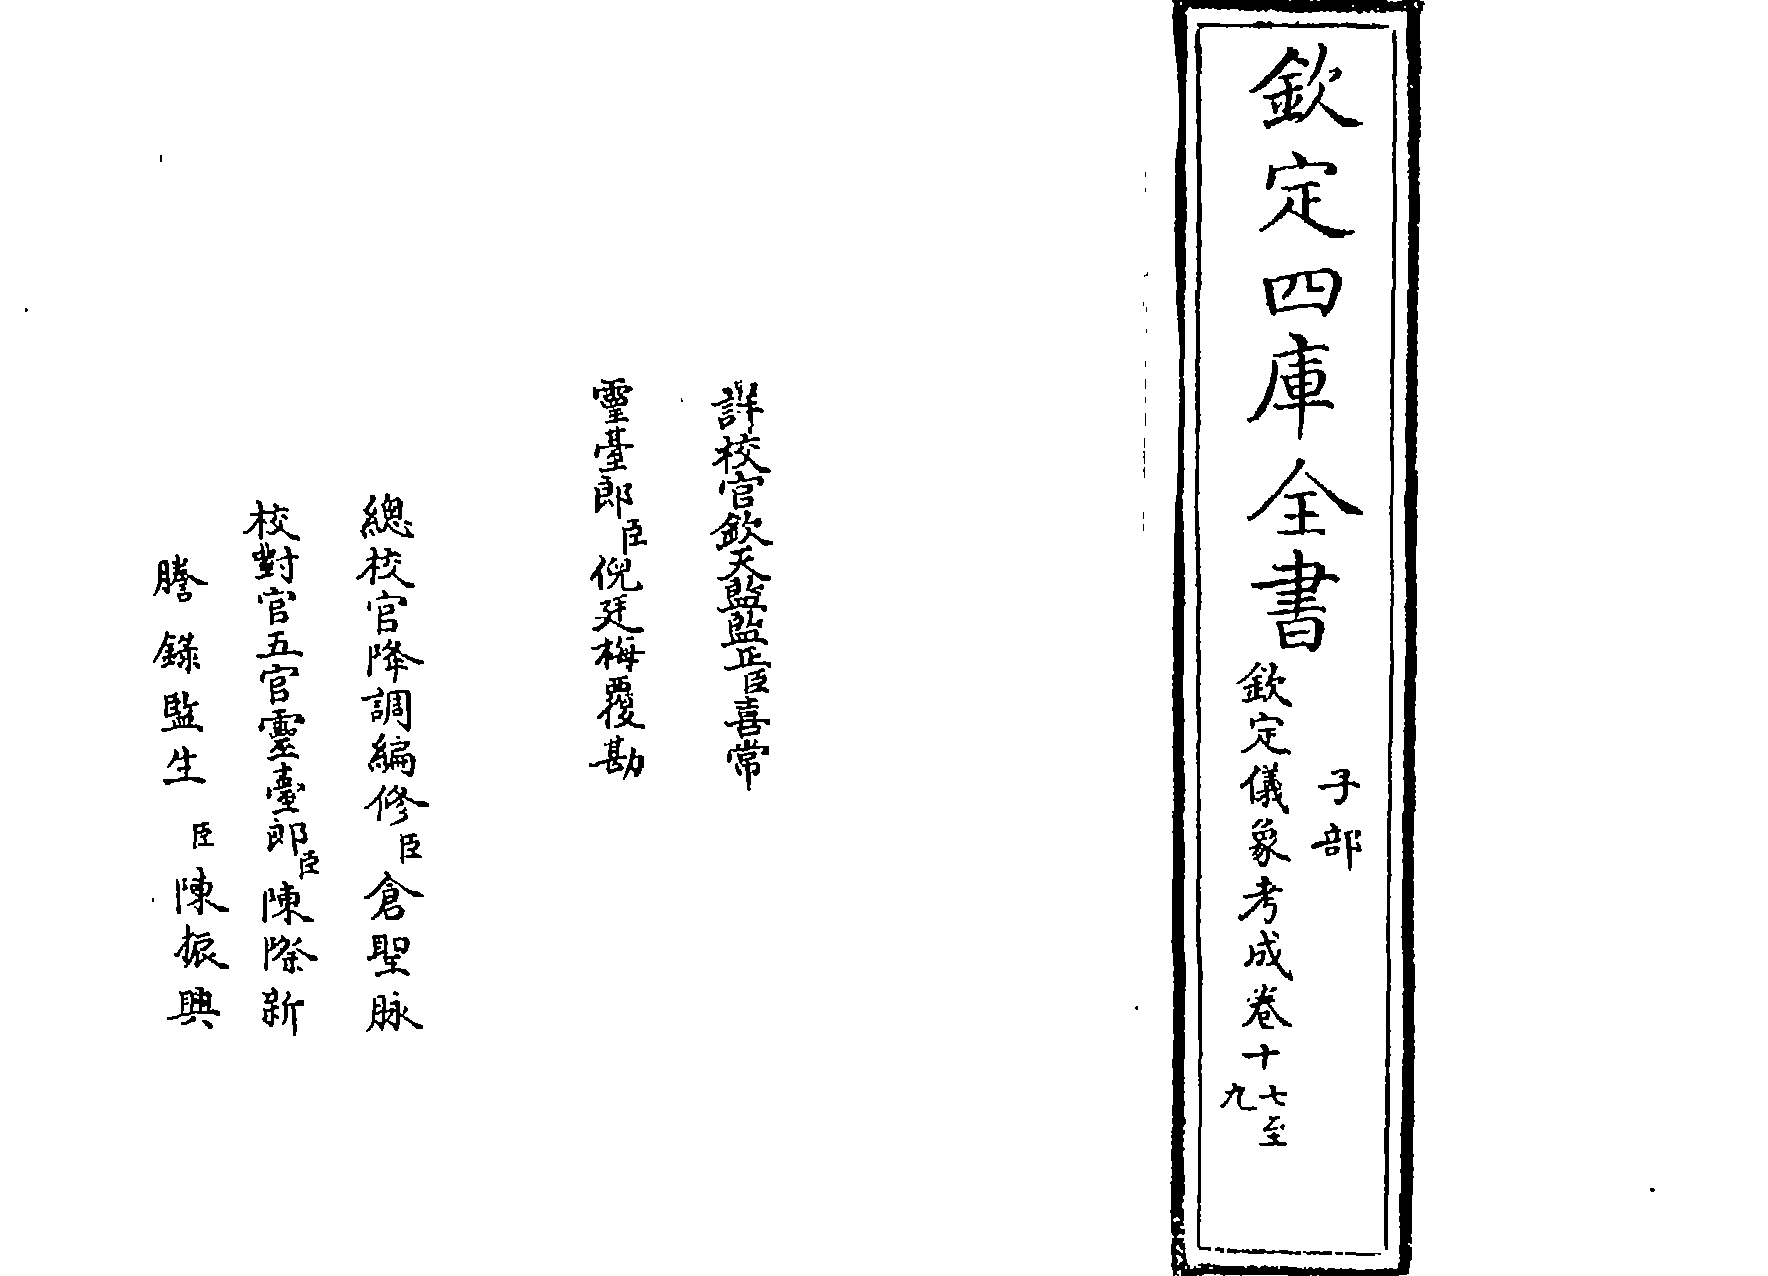
\includegraphics[width=\paperwidth,height=\paperheight,keepaspectratio]{img/1152.png}\clearpage
\begin{正文}
% ---- 册793 葉1153 ----
\SetPageNumber{1}
欽定四庫全書\换行
欽定儀象考成卷十七\换行
　恒星赤道經緯度表四\换行
　　赤道降婁宫\双列{\右小列{黄道度附}\左小列{}}\换行
\char"200B\relax\换行
\char"200B\relax\换行
\char"200B\relax\换行
\char"200B\relax\换行
\char"200B\relax\换行
\char"200B\relax\换行
\char"200B\relax\换行
\char"200B\relax\换行
\char"200B\relax\换行
\char"200B\relax\换行
\char"200B\relax\换行
\char"200B\relax
\par
\end{正文}\clearpage
\嵌图{146.67pt}{202.46pt}{838.42pt}{584.87pt}{img/1156.png}
\begin{正文}
% ---- 册793 葉1156 图版 ----
\SetPageNumber{2}
\插图页
\char"200B\relax\换行
\char"200B\relax\换行
\char"200B\relax\换行
\char"200B\relax\换行
\char"200B\relax\换行
\char"200B\relax\换行
\char"200B\relax\换行
\char"200B\relax\换行
\char"200B\relax\换行
\char"200B\relax\换行
\char"200B\relax\换行
\char"200B\relax\换行
\char"200B\relax\换行
\char"200B\relax\换行
\char"200B\relax\换行
\char"200B\relax
\恢复丝栏\par
\end{正文}\clearpage
\嵌图{148.67pt}{202.87pt}{834.42pt}{584.06pt}{img/1157.png}
\begin{正文}
% ---- 册793 葉1157 图版 ----
\SetPageNumber{3}
\插图页
\char"200B\relax\换行
\char"200B\relax\换行
\char"200B\relax\换行
\char"200B\relax\换行
\char"200B\relax\换行
\char"200B\relax\换行
\char"200B\relax\换行
\char"200B\relax\换行
\char"200B\relax\换行
\char"200B\relax\换行
\char"200B\relax\换行
\char"200B\relax\换行
\char"200B\relax\换行
\char"200B\relax\换行
\char"200B\relax\换行
\char"200B\relax
\恢复丝栏\par
\end{正文}\clearpage
\嵌图{142.64pt}{201.97pt}{846.47pt}{585.85pt}{img/1160.png}
\begin{正文}
% ---- 册793 葉1160 图版 ----
\SetPageNumber{4}
\插图页
\char"200B\relax\换行
\char"200B\relax\换行
\char"200B\relax\换行
\char"200B\relax\换行
\char"200B\relax\换行
\char"200B\relax\换行
\char"200B\relax\换行
\char"200B\relax\换行
\char"200B\relax\换行
\char"200B\relax\换行
\char"200B\relax\换行
\char"200B\relax\换行
\char"200B\relax\换行
\char"200B\relax\换行
\char"200B\relax\换行
\char"200B\relax
\恢复丝栏\par
\end{正文}\clearpage
\嵌图{146.62pt}{202.89pt}{838.53pt}{584.00pt}{img/1161.png}
\begin{正文}
% ---- 册793 葉1161 图版 ----
\SetPageNumber{5}
\插图页
\char"200B\relax\换行
\char"200B\relax\换行
\char"200B\relax\换行
\char"200B\relax\换行
\char"200B\relax\换行
\char"200B\relax\换行
\char"200B\relax\换行
\char"200B\relax\换行
\char"200B\relax\换行
\char"200B\relax\换行
\char"200B\relax\换行
\char"200B\relax\换行
\char"200B\relax\换行
\char"200B\relax\换行
\char"200B\relax\换行
\char"200B\relax
\恢复丝栏\par
\end{正文}\clearpage
\嵌图{144.63pt}{201.02pt}{842.50pt}{587.76pt}{img/1164.png}
\begin{正文}
% ---- 册793 葉1164 图版 ----
\SetPageNumber{6}
\插图页
\char"200B\relax\换行
\char"200B\relax\换行
\char"200B\relax\换行
\char"200B\relax\换行
\char"200B\relax\换行
\char"200B\relax\换行
\char"200B\relax\换行
\char"200B\relax\换行
\char"200B\relax\换行
\char"200B\relax\换行
\char"200B\relax\换行
\char"200B\relax\换行
\char"200B\relax\换行
\char"200B\relax\换行
\char"200B\relax\换行
\char"200B\relax
\恢复丝栏\par
\end{正文}\clearpage
\嵌图{146.62pt}{203.80pt}{838.53pt}{582.19pt}{img/1165.png}
\begin{正文}
% ---- 册793 葉1165 图版 ----
\SetPageNumber{7}
\插图页
\char"200B\relax\换行
\char"200B\relax\换行
\char"200B\relax\换行
\char"200B\relax\换行
\char"200B\relax\换行
\char"200B\relax\换行
\char"200B\relax\换行
\char"200B\relax\换行
\char"200B\relax\换行
\char"200B\relax\换行
\char"200B\relax\换行
\char"200B\relax\换行
\char"200B\relax\换行
\char"200B\relax\换行
\char"200B\relax\换行
\char"200B\relax
\恢复丝栏\par
\end{正文}\clearpage
\嵌图{140.71pt}{205.34pt}{850.34pt}{579.11pt}{img/1168.png}
\begin{正文}
% ---- 册793 葉1168 图版 ----
\SetPageNumber{8}
\插图页
\char"200B\relax\换行
\char"200B\relax\换行
\char"200B\relax\换行
\char"200B\relax\换行
\char"200B\relax\换行
\char"200B\relax\换行
\char"200B\relax\换行
\char"200B\relax\换行
\char"200B\relax\换行
\char"200B\relax\换行
\char"200B\relax\换行
\char"200B\relax\换行
\char"200B\relax\换行
\char"200B\relax\换行
\char"200B\relax\换行
\char"200B\relax
\恢复丝栏\par
\end{正文}\clearpage
\嵌图{142.72pt}{202.02pt}{846.33pt}{585.75pt}{img/1169.png}
\begin{正文}
% ---- 册793 葉1169 图版 ----
\SetPageNumber{9}
\插图页
\char"200B\relax\换行
\char"200B\relax\换行
\char"200B\relax\换行
\char"200B\relax\换行
\char"200B\relax\换行
\char"200B\relax\换行
\char"200B\relax\换行
\char"200B\relax\换行
\char"200B\relax\换行
\char"200B\relax\换行
\char"200B\relax\换行
\char"200B\relax\换行
\char"200B\relax\换行
\char"200B\relax\换行
\char"200B\relax\换行
\char"200B\relax
\恢复丝栏\par
\end{正文}\clearpage
\嵌图{144.63pt}{204.80pt}{842.50pt}{580.18pt}{img/1172.png}
\begin{正文}
% ---- 册793 葉1172 图版 ----
\SetPageNumber{10}
\插图页
\char"200B\relax\换行
\char"200B\relax\换行
\char"200B\relax\换行
\char"200B\relax\换行
\char"200B\relax\换行
\char"200B\relax\换行
\char"200B\relax\换行
\char"200B\relax\换行
\char"200B\relax\换行
\char"200B\relax\换行
\char"200B\relax\换行
\char"200B\relax\换行
\char"200B\relax\换行
\char"200B\relax\换行
\char"200B\relax\换行
\char"200B\relax
\恢复丝栏\par
\end{正文}\clearpage
\嵌图{146.62pt}{203.78pt}{838.53pt}{582.23pt}{img/1173.png}
\begin{正文}
% ---- 册793 葉1173 图版 ----
\SetPageNumber{11}
\插图页
\char"200B\relax\换行
\char"200B\relax\换行
\char"200B\relax\换行
\char"200B\relax\换行
\char"200B\relax\换行
\char"200B\relax\换行
\char"200B\relax\换行
\char"200B\relax\换行
\char"200B\relax\换行
\char"200B\relax\换行
\char"200B\relax\换行
\char"200B\relax\换行
\char"200B\relax\换行
\char"200B\relax\换行
\char"200B\relax\换行
\char"200B\relax
\恢复丝栏\par
\end{正文}\clearpage
\嵌图{140.68pt}{203.00pt}{850.39pt}{583.79pt}{img/1176.png}
\begin{正文}
% ---- 册793 葉1176 图版 ----
\SetPageNumber{12}
\插图页
\char"200B\relax\换行
\char"200B\relax\换行
\char"200B\relax\换行
\char"200B\relax\换行
\char"200B\relax\换行
\char"200B\relax\换行
\char"200B\relax\换行
\char"200B\relax\换行
\char"200B\relax\换行
\char"200B\relax\换行
\char"200B\relax\换行
\char"200B\relax\换行
\char"200B\relax\换行
\char"200B\relax\换行
\char"200B\relax\换行
\char"200B\relax
\恢复丝栏\par
\end{正文}\clearpage
\嵌图{142.68pt}{202.50pt}{846.40pt}{584.78pt}{img/1177.png}
\begin{正文}
% ---- 册793 葉1177 图版 ----
\SetPageNumber{13}
\插图页
\char"200B\relax\换行
\char"200B\relax\换行
\char"200B\relax\换行
\char"200B\relax\换行
\char"200B\relax\换行
\char"200B\relax\换行
\char"200B\relax\换行
\char"200B\relax\换行
\char"200B\relax\换行
\char"200B\relax\换行
\char"200B\relax\换行
\char"200B\relax\换行
\char"200B\relax\换行
\char"200B\relax\换行
\char"200B\relax\换行
\char"200B\relax
\恢复丝栏\par
\end{正文}\clearpage
\嵌图{144.68pt}{203.81pt}{842.41pt}{582.17pt}{img/1180.png}
\begin{正文}
% ---- 册793 葉1180 图版 ----
\SetPageNumber{14}
\插图页
\char"200B\relax\换行
\char"200B\relax\换行
\char"200B\relax\换行
\char"200B\relax\换行
\char"200B\relax\换行
\char"200B\relax\换行
\char"200B\relax\换行
\char"200B\relax\换行
\char"200B\relax\换行
\char"200B\relax\换行
\char"200B\relax\换行
\char"200B\relax\换行
\char"200B\relax\换行
\char"200B\relax\换行
\char"200B\relax\换行
\char"200B\relax
\恢复丝栏\par
\end{正文}\clearpage
\嵌图{144.68pt}{202.45pt}{842.41pt}{584.88pt}{img/1181.png}
\begin{正文}
% ---- 册793 葉1181 图版 ----
\SetPageNumber{15}
\插图页
\char"200B\relax\换行
\char"200B\relax\换行
\char"200B\relax\换行
\char"200B\relax\换行
\char"200B\relax\换行
\char"200B\relax\换行
\char"200B\relax\换行
\char"200B\relax\换行
\char"200B\relax\换行
\char"200B\relax\换行
\char"200B\relax\换行
\char"200B\relax\换行
\char"200B\relax\换行
\char"200B\relax\换行
\char"200B\relax\换行
\char"200B\relax
\恢复丝栏\par
\end{正文}\clearpage
\嵌图{140.66pt}{201.50pt}{850.45pt}{586.80pt}{img/1184.png}
\begin{正文}
% ---- 册793 葉1184 图版 ----
\SetPageNumber{16}
\插图页
\char"200B\relax\换行
\char"200B\relax\换行
\char"200B\relax\换行
\char"200B\relax\换行
\char"200B\relax\换行
\char"200B\relax\换行
\char"200B\relax\换行
\char"200B\relax\换行
\char"200B\relax\换行
\char"200B\relax\换行
\char"200B\relax\换行
\char"200B\relax\换行
\char"200B\relax\换行
\char"200B\relax\换行
\char"200B\relax\换行
\char"200B\relax
\恢复丝栏\par
\end{正文}\clearpage
\嵌图{142.64pt}{201.51pt}{846.47pt}{586.77pt}{img/1185.png}
\begin{正文}
% ---- 册793 葉1185 图版 ----
\SetPageNumber{17}
\插图页
\char"200B\relax\换行
\char"200B\relax\换行
\char"200B\relax\换行
\char"200B\relax\换行
\char"200B\relax\换行
\char"200B\relax\换行
\char"200B\relax\换行
\char"200B\relax\换行
\char"200B\relax\换行
\char"200B\relax\换行
\char"200B\relax\换行
\char"200B\relax\换行
\char"200B\relax\换行
\char"200B\relax\换行
\char"200B\relax\换行
\char"200B\relax
\恢复丝栏\par
\end{正文}\clearpage
\嵌图{146.67pt}{201.02pt}{838.42pt}{587.74pt}{img/1188.png}
\begin{正文}
% ---- 册793 葉1188 图版 ----
\SetPageNumber{18}
\插图页
\char"200B\relax\换行
\char"200B\relax\换行
\char"200B\relax\换行
\char"200B\relax\换行
\char"200B\relax\换行
\char"200B\relax\换行
\char"200B\relax\换行
\char"200B\relax\换行
\char"200B\relax\换行
\char"200B\relax\换行
\char"200B\relax\换行
\char"200B\relax\换行
\char"200B\relax\换行
\char"200B\relax\换行
\char"200B\relax\换行
\char"200B\relax
\恢复丝栏\par
\end{正文}\clearpage
\嵌图{146.67pt}{202.92pt}{838.42pt}{583.95pt}{img/1189.png}
\begin{正文}
% ---- 册793 葉1189 图版 ----
\SetPageNumber{19}
\插图页
\char"200B\relax\换行
\char"200B\relax\换行
\char"200B\relax\换行
\char"200B\relax\换行
\char"200B\relax\换行
\char"200B\relax\换行
\char"200B\relax\换行
\char"200B\relax\换行
\char"200B\relax\换行
\char"200B\relax\换行
\char"200B\relax\换行
\char"200B\relax\换行
\char"200B\relax\换行
\char"200B\relax\换行
\char"200B\relax\换行
\char"200B\relax
\恢复丝栏\par
\end{正文}\clearpage
\嵌图{150.30pt}{206.70pt}{831.15pt}{576.39pt}{img/1192.png}
\begin{正文}
% ---- 册793 葉1192 图版 ----
\SetPageNumber{20}
\插图页
\char"200B\relax\换行
\char"200B\relax\换行
\char"200B\relax\换行
\char"200B\relax\换行
\char"200B\relax\换行
\char"200B\relax\换行
\char"200B\relax\换行
\char"200B\relax\换行
\char"200B\relax\换行
\char"200B\relax\换行
\char"200B\relax\换行
\char"200B\relax\换行
\char"200B\relax\换行
\char"200B\relax\换行
\char"200B\relax\换行
\char"200B\relax
\恢复丝栏\par
\end{正文}\clearpage
\嵌图{193.20pt}{210.32pt}{543.58pt}{582.51pt}{img/1193.png}
\begin{正文}
% ---- 册793 葉1193 ----
\SetPageNumber{21}
\插图页
\char"200B\relax\换行
\char"200B\relax\换行
\char"200B\relax\换行
\char"200B\relax\换行
\char"200B\relax\换行
\char"200B\relax\换行
\char"200B\relax\换行
\char"200B\relax\换行
\恢复丝栏
\char"200B\relax\换行
\char"200B\relax\换行
\char"200B\relax\换行
\char"200B\relax\换行
\char"200B\relax\换行
\char"200B\relax\换行
\char"200B\relax\换行
欽定儀象考成卷十七
\par

% ======== 卷十八（8行21字）========
\par\end{正文}\clearpage
\chapter*{欽定儀象考成卷十八}
\begin{正文}
% ---- 册793 葉1196 ----
\SetPageNumber{1}
欽定四庫全書\换行
欽定儀象考成卷十八\换行
　恒星赤道經緯度表五\换行
　　赤道大梁宫\双列{\右小列{黄道度附}\左小列{}}\换行
\char"200B\relax\换行
\char"200B\relax\换行
\char"200B\relax\换行
\char"200B\relax\换行
\char"200B\relax\换行
\char"200B\relax\换行
\char"200B\relax\换行
\char"200B\relax\换行
\char"200B\relax\换行
\char"200B\relax\换行
\char"200B\relax\换行
\char"200B\relax
\par
\end{正文}\clearpage
\嵌图{144.63pt}{202.85pt}{842.50pt}{584.09pt}{img/1197.png}
\begin{正文}
% ---- 册793 葉1197 图版 ----
\SetPageNumber{2}
\插图页
\char"200B\relax\换行
\char"200B\relax\换行
\char"200B\relax\换行
\char"200B\relax\换行
\char"200B\relax\换行
\char"200B\relax\换行
\char"200B\relax\换行
\char"200B\relax\换行
\char"200B\relax\换行
\char"200B\relax\换行
\char"200B\relax\换行
\char"200B\relax\换行
\char"200B\relax\换行
\char"200B\relax\换行
\char"200B\relax\换行
\char"200B\relax
\恢复丝栏\par
\end{正文}\clearpage
\嵌图{142.68pt}{201.56pt}{846.40pt}{586.67pt}{img/1200.png}
\begin{正文}
% ---- 册793 葉1200 图版 ----
\SetPageNumber{3}
\插图页
\char"200B\relax\换行
\char"200B\relax\换行
\char"200B\relax\换行
\char"200B\relax\换行
\char"200B\relax\换行
\char"200B\relax\换行
\char"200B\relax\换行
\char"200B\relax\换行
\char"200B\relax\换行
\char"200B\relax\换行
\char"200B\relax\换行
\char"200B\relax\换行
\char"200B\relax\换行
\char"200B\relax\换行
\char"200B\relax\换行
\char"200B\relax
\恢复丝栏\par
\end{正文}\clearpage
\嵌图{142.68pt}{202.49pt}{846.40pt}{584.80pt}{img/1201.png}
\begin{正文}
% ---- 册793 葉1201 图版 ----
\SetPageNumber{4}
\插图页
\char"200B\relax\换行
\char"200B\relax\换行
\char"200B\relax\换行
\char"200B\relax\换行
\char"200B\relax\换行
\char"200B\relax\换行
\char"200B\relax\换行
\char"200B\relax\换行
\char"200B\relax\换行
\char"200B\relax\换行
\char"200B\relax\换行
\char"200B\relax\换行
\char"200B\relax\换行
\char"200B\relax\换行
\char"200B\relax\换行
\char"200B\relax
\恢复丝栏\par
\end{正文}\clearpage
\嵌图{146.62pt}{201.48pt}{838.53pt}{586.83pt}{img/1204.png}
\begin{正文}
% ---- 册793 葉1204 图版 ----
\SetPageNumber{5}
\插图页
\char"200B\relax\换行
\char"200B\relax\换行
\char"200B\relax\换行
\char"200B\relax\换行
\char"200B\relax\换行
\char"200B\relax\换行
\char"200B\relax\换行
\char"200B\relax\换行
\char"200B\relax\换行
\char"200B\relax\换行
\char"200B\relax\换行
\char"200B\relax\换行
\char"200B\relax\换行
\char"200B\relax\换行
\char"200B\relax\换行
\char"200B\relax
\恢复丝栏\par
\end{正文}\clearpage
\嵌图{146.62pt}{201.01pt}{838.53pt}{587.77pt}{img/1205.png}
\begin{正文}
% ---- 册793 葉1205 图版 ----
\SetPageNumber{6}
\插图页
\char"200B\relax\换行
\char"200B\relax\换行
\char"200B\relax\换行
\char"200B\relax\换行
\char"200B\relax\换行
\char"200B\relax\换行
\char"200B\relax\换行
\char"200B\relax\换行
\char"200B\relax\换行
\char"200B\relax\换行
\char"200B\relax\换行
\char"200B\relax\换行
\char"200B\relax\换行
\char"200B\relax\换行
\char"200B\relax\换行
\char"200B\relax
\恢复丝栏\par
\end{正文}\clearpage
\嵌图{144.68pt}{201.57pt}{842.41pt}{586.66pt}{img/1208.png}
\begin{正文}
% ---- 册793 葉1208 图版 ----
\SetPageNumber{7}
\插图页
\char"200B\relax\换行
\char"200B\relax\换行
\char"200B\relax\换行
\char"200B\relax\换行
\char"200B\relax\换行
\char"200B\relax\换行
\char"200B\relax\换行
\char"200B\relax\换行
\char"200B\relax\换行
\char"200B\relax\换行
\char"200B\relax\换行
\char"200B\relax\换行
\char"200B\relax\换行
\char"200B\relax\换行
\char"200B\relax\换行
\char"200B\relax
\恢复丝栏\par
\end{正文}\clearpage
\嵌图{142.68pt}{202.52pt}{846.40pt}{584.75pt}{img/1209.png}
\begin{正文}
% ---- 册793 葉1209 图版 ----
\SetPageNumber{8}
\插图页
\char"200B\relax\换行
\char"200B\relax\换行
\char"200B\relax\换行
\char"200B\relax\换行
\char"200B\relax\换行
\char"200B\relax\换行
\char"200B\relax\换行
\char"200B\relax\换行
\char"200B\relax\换行
\char"200B\relax\换行
\char"200B\relax\换行
\char"200B\relax\换行
\char"200B\relax\换行
\char"200B\relax\换行
\char"200B\relax\换行
\char"200B\relax
\恢复丝栏\par
\end{正文}\clearpage
\嵌图{146.67pt}{200.53pt}{838.42pt}{588.73pt}{img/1212.png}
\begin{正文}
% ---- 册793 葉1212 图版 ----
\SetPageNumber{9}
\插图页
\char"200B\relax\换行
\char"200B\relax\换行
\char"200B\relax\换行
\char"200B\relax\换行
\char"200B\relax\换行
\char"200B\relax\换行
\char"200B\relax\换行
\char"200B\relax\换行
\char"200B\relax\换行
\char"200B\relax\换行
\char"200B\relax\换行
\char"200B\relax\换行
\char"200B\relax\换行
\char"200B\relax\换行
\char"200B\relax\换行
\char"200B\relax
\恢复丝栏\par
\end{正文}\clearpage
\嵌图{146.67pt}{201.03pt}{838.42pt}{587.73pt}{img/1213.png}
\begin{正文}
% ---- 册793 葉1213 图版 ----
\SetPageNumber{10}
\插图页
\char"200B\relax\换行
\char"200B\relax\换行
\char"200B\relax\换行
\char"200B\relax\换行
\char"200B\relax\换行
\char"200B\relax\换行
\char"200B\relax\换行
\char"200B\relax\换行
\char"200B\relax\换行
\char"200B\relax\换行
\char"200B\relax\换行
\char"200B\relax\换行
\char"200B\relax\换行
\char"200B\relax\换行
\char"200B\relax\换行
\char"200B\relax
\恢复丝栏\par
\end{正文}\clearpage
\嵌图{148.61pt}{200.57pt}{834.55pt}{588.65pt}{img/1216.png}
\begin{正文}
% ---- 册793 葉1216 图版 ----
\SetPageNumber{11}
\插图页
\char"200B\relax\换行
\char"200B\relax\换行
\char"200B\relax\换行
\char"200B\relax\换行
\char"200B\relax\换行
\char"200B\relax\换行
\char"200B\relax\换行
\char"200B\relax\换行
\char"200B\relax\换行
\char"200B\relax\换行
\char"200B\relax\换行
\char"200B\relax\换行
\char"200B\relax\换行
\char"200B\relax\换行
\char"200B\relax\换行
\char"200B\relax
\恢复丝栏\par
\end{正文}\clearpage
\嵌图{144.63pt}{202.01pt}{842.50pt}{585.77pt}{img/1217.png}
\begin{正文}
% ---- 册793 葉1217 图版 ----
\SetPageNumber{12}
\插图页
\char"200B\relax\换行
\char"200B\relax\换行
\char"200B\relax\换行
\char"200B\relax\换行
\char"200B\relax\换行
\char"200B\relax\换行
\char"200B\relax\换行
\char"200B\relax\换行
\char"200B\relax\换行
\char"200B\relax\换行
\char"200B\relax\换行
\char"200B\relax\换行
\char"200B\relax\换行
\char"200B\relax\换行
\char"200B\relax\换行
\char"200B\relax
\恢复丝栏\par
\end{正文}\clearpage
\嵌图{146.62pt}{200.59pt}{838.53pt}{588.61pt}{img/1220.png}
\begin{正文}
% ---- 册793 葉1220 图版 ----
\SetPageNumber{13}
\插图页
\char"200B\relax\换行
\char"200B\relax\换行
\char"200B\relax\换行
\char"200B\relax\换行
\char"200B\relax\换行
\char"200B\relax\换行
\char"200B\relax\换行
\char"200B\relax\换行
\char"200B\relax\换行
\char"200B\relax\换行
\char"200B\relax\换行
\char"200B\relax\换行
\char"200B\relax\换行
\char"200B\relax\换行
\char"200B\relax\换行
\char"200B\relax
\恢复丝栏\par
\end{正文}\clearpage
\嵌图{144.63pt}{201.02pt}{842.50pt}{587.76pt}{img/1221.png}
\begin{正文}
% ---- 册793 葉1221 图版 ----
\SetPageNumber{14}
\插图页
\char"200B\relax\换行
\char"200B\relax\换行
\char"200B\relax\换行
\char"200B\relax\换行
\char"200B\relax\换行
\char"200B\relax\换行
\char"200B\relax\换行
\char"200B\relax\换行
\char"200B\relax\换行
\char"200B\relax\换行
\char"200B\relax\换行
\char"200B\relax\换行
\char"200B\relax\换行
\char"200B\relax\换行
\char"200B\relax\换行
\char"200B\relax
\恢复丝栏\par
\end{正文}\clearpage
\嵌图{146.56pt}{202.00pt}{838.64pt}{585.78pt}{img/1224.png}
\begin{正文}
% ---- 册793 葉1224 图版 ----
\SetPageNumber{15}
\插图页
\char"200B\relax\换行
\char"200B\relax\换行
\char"200B\relax\换行
\char"200B\relax\换行
\char"200B\relax\换行
\char"200B\relax\换行
\char"200B\relax\换行
\char"200B\relax\换行
\char"200B\relax\换行
\char"200B\relax\换行
\char"200B\relax\换行
\char"200B\relax\换行
\char"200B\relax\换行
\char"200B\relax\换行
\char"200B\relax\换行
\char"200B\relax
\恢复丝栏\par
\end{正文}\clearpage
\嵌图{148.54pt}{200.55pt}{834.68pt}{588.69pt}{img/1225.png}
\begin{正文}
% ---- 册793 葉1225 图版 ----
\SetPageNumber{16}
\插图页
\char"200B\relax\换行
\char"200B\relax\换行
\char"200B\relax\换行
\char"200B\relax\换行
\char"200B\relax\换行
\char"200B\relax\换行
\char"200B\relax\换行
\char"200B\relax\换行
\char"200B\relax\换行
\char"200B\relax\换行
\char"200B\relax\换行
\char"200B\relax\换行
\char"200B\relax\换行
\char"200B\relax\换行
\char"200B\relax\换行
\char"200B\relax
\恢复丝栏\par
\end{正文}\clearpage
\嵌图{146.56pt}{202.93pt}{838.64pt}{583.94pt}{img/1228.png}
\begin{正文}
% ---- 册793 葉1228 图版 ----
\SetPageNumber{17}
\插图页
\char"200B\relax\换行
\char"200B\relax\换行
\char"200B\relax\换行
\char"200B\relax\换行
\char"200B\relax\换行
\char"200B\relax\换行
\char"200B\relax\换行
\char"200B\relax\换行
\char"200B\relax\换行
\char"200B\relax\换行
\char"200B\relax\换行
\char"200B\relax\换行
\char"200B\relax\换行
\char"200B\relax\换行
\char"200B\relax\换行
\char"200B\relax
\恢复丝栏\par
\end{正文}\clearpage
\嵌图{148.54pt}{200.49pt}{834.68pt}{588.80pt}{img/1229.png}
\begin{正文}
% ---- 册793 葉1229 图版 ----
\SetPageNumber{18}
\插图页
\char"200B\relax\换行
\char"200B\relax\换行
\char"200B\relax\换行
\char"200B\relax\换行
\char"200B\relax\换行
\char"200B\relax\换行
\char"200B\relax\换行
\char"200B\relax\换行
\char"200B\relax\换行
\char"200B\relax\换行
\char"200B\relax\换行
\char"200B\relax\换行
\char"200B\relax\换行
\char"200B\relax\换行
\char"200B\relax\换行
\char"200B\relax
\恢复丝栏\par
\end{正文}\clearpage
\嵌图{154.21pt}{201.07pt}{823.35pt}{587.64pt}{img/1232.png}
\begin{正文}
% ---- 册793 葉1232 图版 ----
\SetPageNumber{19}
\插图页
\char"200B\relax\换行
\char"200B\relax\换行
\char"200B\relax\换行
\char"200B\relax\换行
\char"200B\relax\换行
\char"200B\relax\换行
\char"200B\relax\换行
\char"200B\relax\换行
\char"200B\relax\换行
\char"200B\relax\换行
\char"200B\relax\换行
\char"200B\relax\换行
\char"200B\relax\换行
\char"200B\relax\换行
\char"200B\relax\换行
\char"200B\relax
\恢复丝栏\par
\end{正文}\clearpage
\嵌图{170.46pt}{235.03pt}{173.48pt}{586.18pt}{img/1233.png}
\begin{正文}
% ---- 册793 葉1233 ----
\SetPageNumber{20}
\char"200B\relax\换行
\char"200B\relax\换行
\char"200B\relax\换行
\char"200B\relax\换行
\char"200B\relax\换行
\char"200B\relax\换行
\char"200B\relax\换行
\char"200B\relax\换行
\char"200B\relax\换行
\char"200B\relax\换行
\char"200B\relax\换行
\char"200B\relax\换行
\char"200B\relax\换行
\char"200B\relax\换行
\char"200B\relax\换行
欽定儀象考成卷十八
\par

% ======== 卷十九（8行21字）========
\par\end{正文}\clearpage
\chapter*{欽定儀象考成卷十九}
\begin{正文}
% ---- 册793 葉1236 ----
\SetPageNumber{1}
欽定四庫全書\换行
欽定儀象考成卷十九\换行
　恒星赤道經緯度表六\换行
　　赤道實沈宫\双列{\右小列{黄道度附}\左小列{}}\换行
\char"200B\relax\换行
\char"200B\relax\换行
\char"200B\relax\换行
\char"200B\relax\换行
\char"200B\relax\换行
\char"200B\relax\换行
\char"200B\relax\换行
\char"200B\relax\换行
\char"200B\relax\换行
\char"200B\relax\换行
\char"200B\relax\换行
\char"200B\relax
\par
\end{正文}\clearpage
\嵌图{146.56pt}{200.07pt}{838.64pt}{589.65pt}{img/1237.png}
\begin{正文}
% ---- 册793 葉1237 图版 ----
\SetPageNumber{2}
\插图页
\char"200B\relax\换行
\char"200B\relax\换行
\char"200B\relax\换行
\char"200B\relax\换行
\char"200B\relax\换行
\char"200B\relax\换行
\char"200B\relax\换行
\char"200B\relax\换行
\char"200B\relax\换行
\char"200B\relax\换行
\char"200B\relax\换行
\char"200B\relax\换行
\char"200B\relax\换行
\char"200B\relax\换行
\char"200B\relax\换行
\char"200B\relax
\恢复丝栏\par
\end{正文}\clearpage
\嵌图{144.63pt}{202.03pt}{842.50pt}{585.74pt}{img/1240.png}
\begin{正文}
% ---- 册793 葉1240 图版 ----
\SetPageNumber{3}
\插图页
\char"200B\relax\换行
\char"200B\relax\换行
\char"200B\relax\换行
\char"200B\relax\换行
\char"200B\relax\换行
\char"200B\relax\换行
\char"200B\relax\换行
\char"200B\relax\换行
\char"200B\relax\换行
\char"200B\relax\换行
\char"200B\relax\换行
\char"200B\relax\换行
\char"200B\relax\换行
\char"200B\relax\换行
\char"200B\relax\换行
\char"200B\relax
\恢复丝栏\par
\end{正文}\clearpage
\嵌图{144.63pt}{200.59pt}{842.50pt}{588.61pt}{img/1241.png}
\begin{正文}
% ---- 册793 葉1241 图版 ----
\SetPageNumber{4}
\插图页
\char"200B\relax\换行
\char"200B\relax\换行
\char"200B\relax\换行
\char"200B\relax\换行
\char"200B\relax\换行
\char"200B\relax\换行
\char"200B\relax\换行
\char"200B\relax\换行
\char"200B\relax\换行
\char"200B\relax\换行
\char"200B\relax\换行
\char"200B\relax\换行
\char"200B\relax\换行
\char"200B\relax\换行
\char"200B\relax\换行
\char"200B\relax
\恢复丝栏\par
\end{正文}\clearpage
\嵌图{144.68pt}{201.56pt}{842.41pt}{586.67pt}{img/1244.png}
\begin{正文}
% ---- 册793 葉1244 图版 ----
\SetPageNumber{5}
\插图页
\char"200B\relax\换行
\char"200B\relax\换行
\char"200B\relax\换行
\char"200B\relax\换行
\char"200B\relax\换行
\char"200B\relax\换行
\char"200B\relax\换行
\char"200B\relax\换行
\char"200B\relax\换行
\char"200B\relax\换行
\char"200B\relax\换行
\char"200B\relax\换行
\char"200B\relax\换行
\char"200B\relax\换行
\char"200B\relax\换行
\char"200B\relax
\恢复丝栏\par
\end{正文}\clearpage
\嵌图{142.68pt}{202.90pt}{846.40pt}{583.99pt}{img/1245.png}
\begin{正文}
% ---- 册793 葉1245 图版 ----
\SetPageNumber{6}
\插图页
\char"200B\relax\换行
\char"200B\relax\换行
\char"200B\relax\换行
\char"200B\relax\换行
\char"200B\relax\换行
\char"200B\relax\换行
\char"200B\relax\换行
\char"200B\relax\换行
\char"200B\relax\换行
\char"200B\relax\换行
\char"200B\relax\换行
\char"200B\relax\换行
\char"200B\relax\换行
\char"200B\relax\换行
\char"200B\relax\换行
\char"200B\relax
\恢复丝栏\par
\end{正文}\clearpage
\嵌图{142.64pt}{203.00pt}{846.47pt}{583.79pt}{img/1248.png}
\begin{正文}
% ---- 册793 葉1248 图版 ----
\SetPageNumber{7}
\插图页
\char"200B\relax\换行
\char"200B\relax\换行
\char"200B\relax\换行
\char"200B\relax\换行
\char"200B\relax\换行
\char"200B\relax\换行
\char"200B\relax\换行
\char"200B\relax\换行
\char"200B\relax\换行
\char"200B\relax\换行
\char"200B\relax\换行
\char"200B\relax\换行
\char"200B\relax\换行
\char"200B\relax\换行
\char"200B\relax\换行
\char"200B\relax
\恢复丝栏\par
\end{正文}\clearpage
\嵌图{146.62pt}{200.59pt}{838.53pt}{588.61pt}{img/1249.png}
\begin{正文}
% ---- 册793 葉1249 图版 ----
\SetPageNumber{8}
\插图页
\char"200B\relax\换行
\char"200B\relax\换行
\char"200B\relax\换行
\char"200B\relax\换行
\char"200B\relax\换行
\char"200B\relax\换行
\char"200B\relax\换行
\char"200B\relax\换行
\char"200B\relax\换行
\char"200B\relax\换行
\char"200B\relax\换行
\char"200B\relax\换行
\char"200B\relax\换行
\char"200B\relax\换行
\char"200B\relax\换行
\char"200B\relax
\恢复丝栏\par
\end{正文}\clearpage
\嵌图{146.62pt}{201.56pt}{838.53pt}{586.67pt}{img/1252.png}
\begin{正文}
% ---- 册793 葉1252 图版 ----
\SetPageNumber{9}
\插图页
\char"200B\relax\换行
\char"200B\relax\换行
\char"200B\relax\换行
\char"200B\relax\换行
\char"200B\relax\换行
\char"200B\relax\换行
\char"200B\relax\换行
\char"200B\relax\换行
\char"200B\relax\换行
\char"200B\relax\换行
\char"200B\relax\换行
\char"200B\relax\换行
\char"200B\relax\换行
\char"200B\relax\换行
\char"200B\relax\换行
\char"200B\relax
\恢复丝栏\par
\end{正文}\clearpage
\嵌图{144.63pt}{201.99pt}{842.50pt}{585.80pt}{img/1253.png}
\begin{正文}
% ---- 册793 葉1253 图版 ----
\SetPageNumber{10}
\插图页
\char"200B\relax\换行
\char"200B\relax\换行
\char"200B\relax\换行
\char"200B\relax\换行
\char"200B\relax\换行
\char"200B\relax\换行
\char"200B\relax\换行
\char"200B\relax\换行
\char"200B\relax\换行
\char"200B\relax\换行
\char"200B\relax\换行
\char"200B\relax\换行
\char"200B\relax\换行
\char"200B\relax\换行
\char"200B\relax\换行
\char"200B\relax
\恢复丝栏\par
\end{正文}\clearpage
\嵌图{144.59pt}{204.41pt}{842.59pt}{580.97pt}{img/1256.png}
\begin{正文}
% ---- 册793 葉1256 图版 ----
\SetPageNumber{11}
\插图页
\char"200B\relax\换行
\char"200B\relax\换行
\char"200B\relax\换行
\char"200B\relax\换行
\char"200B\relax\换行
\char"200B\relax\换行
\char"200B\relax\换行
\char"200B\relax\换行
\char"200B\relax\换行
\char"200B\relax\换行
\char"200B\relax\换行
\char"200B\relax\换行
\char"200B\relax\换行
\char"200B\relax\换行
\char"200B\relax\换行
\char"200B\relax
\恢复丝栏\par
\end{正文}\clearpage
\嵌图{142.61pt}{202.95pt}{846.55pt}{583.88pt}{img/1257.png}
\begin{正文}
% ---- 册793 葉1257 图版 ----
\SetPageNumber{12}
\插图页
\char"200B\relax\换行
\char"200B\relax\换行
\char"200B\relax\换行
\char"200B\relax\换行
\char"200B\relax\换行
\char"200B\relax\换行
\char"200B\relax\换行
\char"200B\relax\换行
\char"200B\relax\换行
\char"200B\relax\换行
\char"200B\relax\换行
\char"200B\relax\换行
\char"200B\relax\换行
\char"200B\relax\换行
\char"200B\relax\换行
\char"200B\relax
\恢复丝栏\par
\end{正文}\clearpage
\嵌图{146.62pt}{202.89pt}{838.53pt}{584.00pt}{img/1260.png}
\begin{正文}
% ---- 册793 葉1260 图版 ----
\SetPageNumber{13}
\插图页
\char"200B\relax\换行
\char"200B\relax\换行
\char"200B\relax\换行
\char"200B\relax\换行
\char"200B\relax\换行
\char"200B\relax\换行
\char"200B\relax\换行
\char"200B\relax\换行
\char"200B\relax\换行
\char"200B\relax\换行
\char"200B\relax\换行
\char"200B\relax\换行
\char"200B\relax\换行
\char"200B\relax\换行
\char"200B\relax\换行
\char"200B\relax
\恢复丝栏\par
\end{正文}\clearpage
\嵌图{142.64pt}{200.99pt}{846.47pt}{587.82pt}{img/1261.png}
\begin{正文}
% ---- 册793 葉1261 图版 ----
\SetPageNumber{14}
\插图页
\char"200B\relax\换行
\char"200B\relax\换行
\char"200B\relax\换行
\char"200B\relax\换行
\char"200B\relax\换行
\char"200B\relax\换行
\char"200B\relax\换行
\char"200B\relax\换行
\char"200B\relax\换行
\char"200B\relax\换行
\char"200B\relax\换行
\char"200B\relax\换行
\char"200B\relax\换行
\char"200B\relax\换行
\char"200B\relax\换行
\char"200B\relax
\恢复丝栏\par
\end{正文}\clearpage
\嵌图{144.63pt}{202.02pt}{842.50pt}{585.75pt}{img/1264.png}
\begin{正文}
% ---- 册793 葉1264 图版 ----
\SetPageNumber{15}
\插图页
\char"200B\relax\换行
\char"200B\relax\换行
\char"200B\relax\换行
\char"200B\relax\换行
\char"200B\relax\换行
\char"200B\relax\换行
\char"200B\relax\换行
\char"200B\relax\换行
\char"200B\relax\换行
\char"200B\relax\换行
\char"200B\relax\换行
\char"200B\relax\换行
\char"200B\relax\换行
\char"200B\relax\换行
\char"200B\relax\换行
\char"200B\relax
\恢复丝栏\par
\end{正文}\clearpage
\嵌图{142.64pt}{200.11pt}{846.47pt}{589.56pt}{img/1265.png}
\begin{正文}
% ---- 册793 葉1265 图版 ----
\SetPageNumber{16}
\插图页
\char"200B\relax\换行
\char"200B\relax\换行
\char"200B\relax\换行
\char"200B\relax\换行
\char"200B\relax\换行
\char"200B\relax\换行
\char"200B\relax\换行
\char"200B\relax\换行
\char"200B\relax\换行
\char"200B\relax\换行
\char"200B\relax\换行
\char"200B\relax\换行
\char"200B\relax\换行
\char"200B\relax\换行
\char"200B\relax\换行
\char"200B\relax
\恢复丝栏\par
\end{正文}\clearpage
\嵌图{144.59pt}{202.46pt}{842.59pt}{584.87pt}{img/1268.png}
\begin{正文}
% ---- 册793 葉1268 图版 ----
\SetPageNumber{17}
\插图页
\char"200B\relax\换行
\char"200B\relax\换行
\char"200B\relax\换行
\char"200B\relax\换行
\char"200B\relax\换行
\char"200B\relax\换行
\char"200B\relax\换行
\char"200B\relax\换行
\char"200B\relax\换行
\char"200B\relax\换行
\char"200B\relax\换行
\char"200B\relax\换行
\char"200B\relax\换行
\char"200B\relax\换行
\char"200B\relax\换行
\char"200B\relax
\恢复丝栏\par
\end{正文}\clearpage
\嵌图{144.59pt}{202.42pt}{842.59pt}{584.95pt}{img/1269.png}
\begin{正文}
% ---- 册793 葉1269 图版 ----
\SetPageNumber{18}
\插图页
\char"200B\relax\换行
\char"200B\relax\换行
\char"200B\relax\换行
\char"200B\relax\换行
\char"200B\relax\换行
\char"200B\relax\换行
\char"200B\relax\换行
\char"200B\relax\换行
\char"200B\relax\换行
\char"200B\relax\换行
\char"200B\relax\换行
\char"200B\relax\换行
\char"200B\relax\换行
\char"200B\relax\换行
\char"200B\relax\换行
\char"200B\relax
\恢复丝栏\par
\end{正文}\clearpage
\嵌图{148.61pt}{199.14pt}{834.55pt}{591.51pt}{img/1272.png}
\begin{正文}
% ---- 册793 葉1272 图版 ----
\SetPageNumber{19}
\插图页
\char"200B\relax\换行
\char"200B\relax\换行
\char"200B\relax\换行
\char"200B\relax\换行
\char"200B\relax\换行
\char"200B\relax\换行
\char"200B\relax\换行
\char"200B\relax\换行
\char"200B\relax\换行
\char"200B\relax\换行
\char"200B\relax\换行
\char"200B\relax\换行
\char"200B\relax\换行
\char"200B\relax\换行
\char"200B\relax\换行
\char"200B\relax
\恢复丝栏\par
\end{正文}\clearpage
\嵌图{146.62pt}{199.59pt}{838.53pt}{590.60pt}{img/1273.png}
\begin{正文}
% ---- 册793 葉1273 图版 ----
\SetPageNumber{20}
\插图页
\char"200B\relax\换行
\char"200B\relax\换行
\char"200B\relax\换行
\char"200B\relax\换行
\char"200B\relax\换行
\char"200B\relax\换行
\char"200B\relax\换行
\char"200B\relax\换行
\char"200B\relax\换行
\char"200B\relax\换行
\char"200B\relax\换行
\char"200B\relax\换行
\char"200B\relax\换行
\char"200B\relax\换行
\char"200B\relax\换行
\char"200B\relax
\恢复丝栏\par
\end{正文}\clearpage
\嵌图{144.68pt}{202.50pt}{842.41pt}{584.78pt}{img/1276.png}
\begin{正文}
% ---- 册793 葉1276 图版 ----
\SetPageNumber{21}
\插图页
\char"200B\relax\换行
\char"200B\relax\换行
\char"200B\relax\换行
\char"200B\relax\换行
\char"200B\relax\换行
\char"200B\relax\换行
\char"200B\relax\换行
\char"200B\relax\换行
\char"200B\relax\换行
\char"200B\relax\换行
\char"200B\relax\换行
\char"200B\relax\换行
\char"200B\relax\换行
\char"200B\relax\换行
\char"200B\relax\换行
\char"200B\relax
\恢复丝栏\par
\end{正文}\clearpage
\嵌图{146.67pt}{201.04pt}{838.42pt}{587.72pt}{img/1277.png}
\begin{正文}
% ---- 册793 葉1277 图版 ----
\SetPageNumber{22}
\插图页
\char"200B\relax\换行
\char"200B\relax\换行
\char"200B\relax\换行
\char"200B\relax\换行
\char"200B\relax\换行
\char"200B\relax\换行
\char"200B\relax\换行
\char"200B\relax\换行
\char"200B\relax\换行
\char"200B\relax\换行
\char"200B\relax\换行
\char"200B\relax\换行
\char"200B\relax\换行
\char"200B\relax\换行
\char"200B\relax\换行
\char"200B\relax
\恢复丝栏\par
\end{正文}\clearpage
\嵌图{148.42pt}{200.55pt}{834.93pt}{588.69pt}{img/1280.png}
\begin{正文}
% ---- 册793 葉1280 图版 ----
\SetPageNumber{23}
\插图页
\char"200B\relax\换行
\char"200B\relax\换行
\char"200B\relax\换行
\char"200B\relax\换行
\char"200B\relax\换行
\char"200B\relax\换行
\char"200B\relax\换行
\char"200B\relax\换行
\char"200B\relax\换行
\char"200B\relax\换行
\char"200B\relax\换行
\char"200B\relax\换行
\char"200B\relax\换行
\char"200B\relax\换行
\char"200B\relax\换行
\char"200B\relax
\恢复丝栏\par
\end{正文}\clearpage
\嵌图{141.38pt}{220.50pt}{406.64pt}{572.33pt}{img/1281.png}
\begin{正文}
% ---- 册793 葉1281 ----
\SetPageNumber{24}
\插图页
\char"200B\relax\换行
\char"200B\relax\换行
\char"200B\relax\换行
\char"200B\relax\换行
\char"200B\relax\换行
\char"200B\relax\换行
\char"200B\relax\换行
\char"200B\relax\换行
\恢复丝栏
\char"200B\relax\换行
\char"200B\relax\换行
\char"200B\relax\换行
\char"200B\relax\换行
\char"200B\relax\换行
\char"200B\relax\换行
\char"200B\relax\换行
欽定儀象考成卷十九
\par

% ======== 卷二十（8行21字）========
\par\end{正文}\clearpage
\chapter*{欽定儀象考成卷二十}
\begin{正文}
\end{正文}\clearpage

  \thispagestyle{empty}\noindent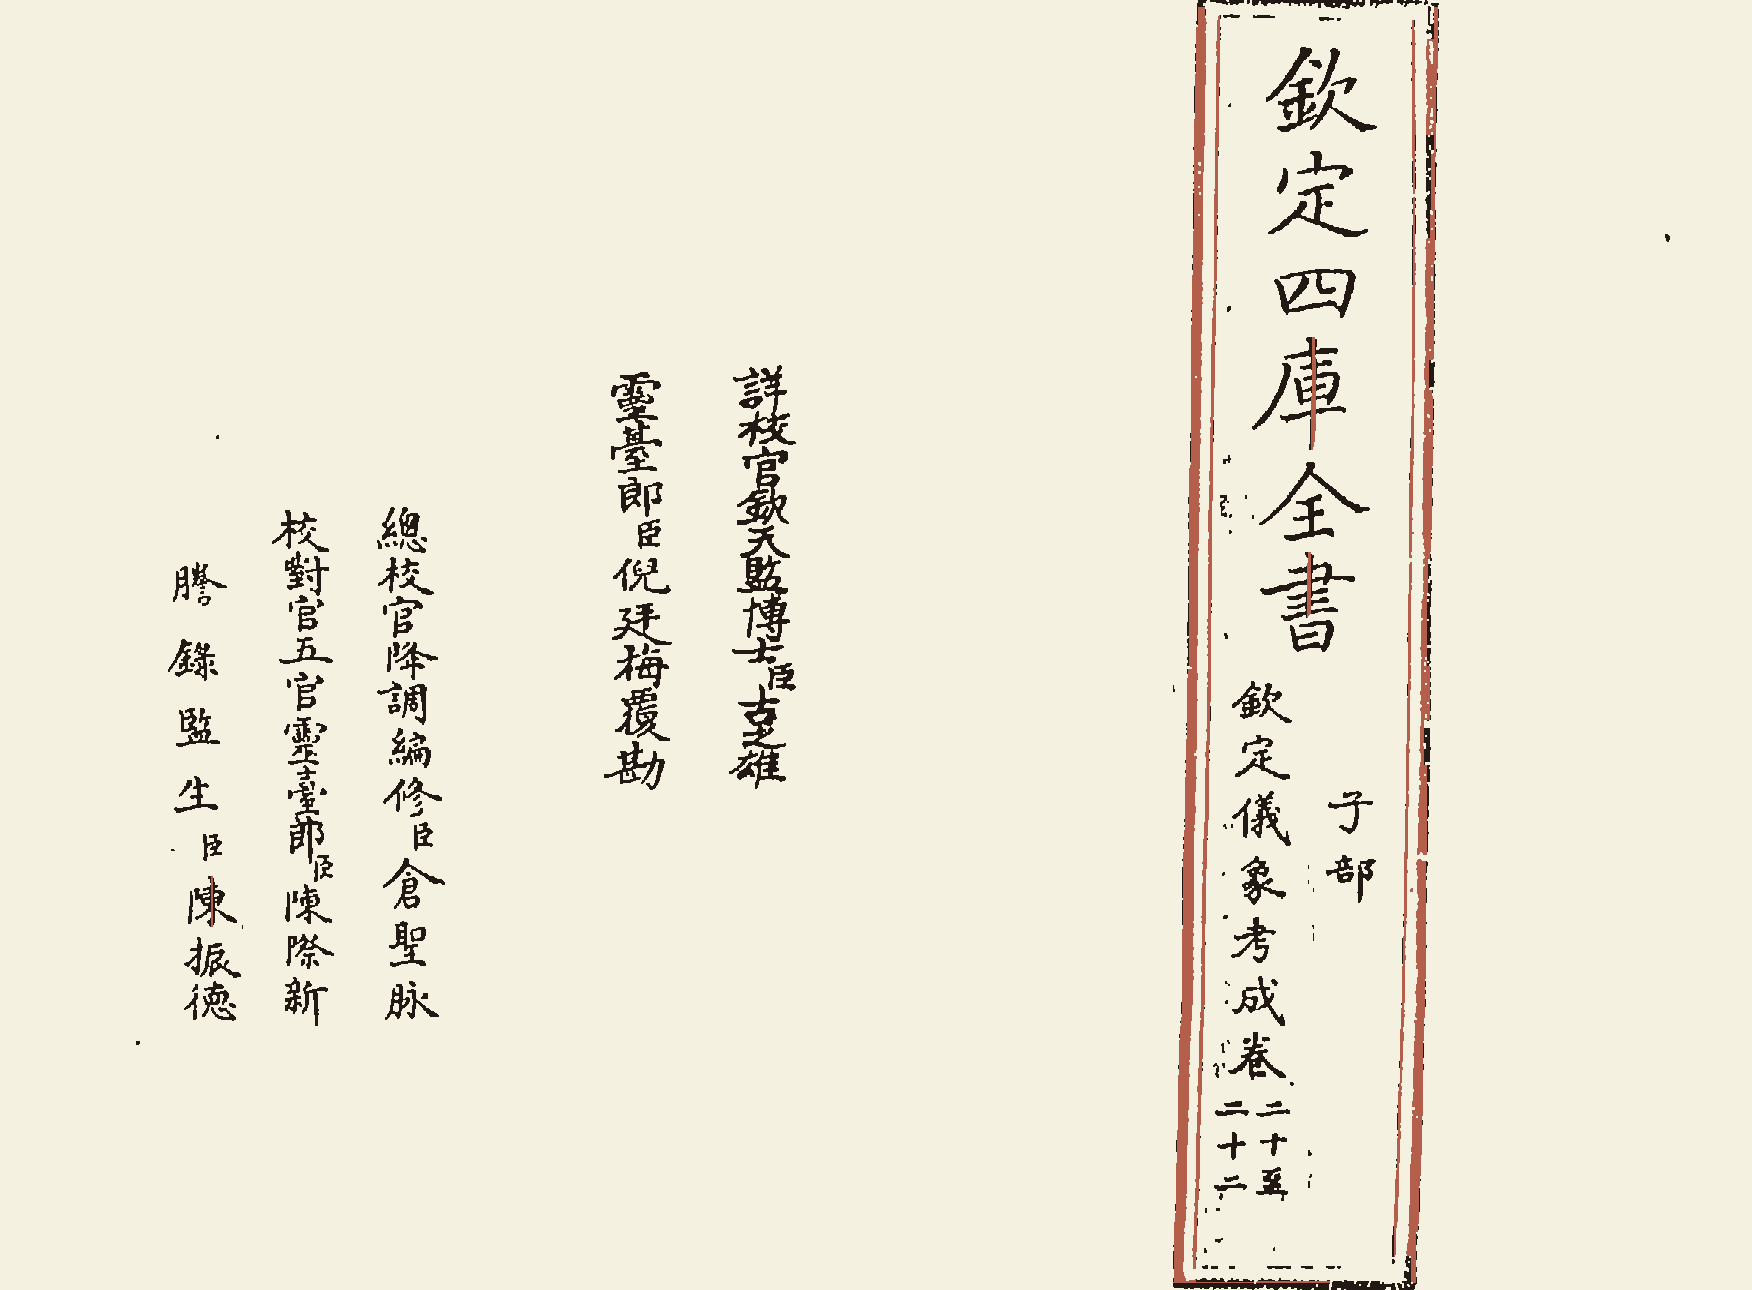
\includegraphics[width=\paperwidth,height=\paperheight,keepaspectratio]{img/1284.png}\clearpage
\begin{正文}
% ---- 册793 葉1285 ----
\SetPageNumber{1}
欽定四庫全書\换行
欽定儀象考成卷二十\换行
　恒星赤道經緯度表七\换行
　　赤道鶉首宫\双列{\右小列{黄道度附}\左小列{}}\换行
\char"200B\relax\换行
\char"200B\relax\换行
\char"200B\relax\换行
\char"200B\relax\换行
\char"200B\relax\换行
\char"200B\relax\换行
\char"200B\relax\换行
\char"200B\relax\换行
\char"200B\relax\换行
\char"200B\relax\换行
\char"200B\relax\换行
\char"200B\relax
\par
\end{正文}\clearpage
\嵌图{142.57pt}{201.98pt}{846.62pt}{585.83pt}{img/1288.png}
\begin{正文}
% ---- 册793 葉1288 图版 ----
\SetPageNumber{2}
\插图页
\char"200B\relax\换行
\char"200B\relax\换行
\char"200B\relax\换行
\char"200B\relax\换行
\char"200B\relax\换行
\char"200B\relax\换行
\char"200B\relax\换行
\char"200B\relax\换行
\char"200B\relax\换行
\char"200B\relax\换行
\char"200B\relax\换行
\char"200B\relax\换行
\char"200B\relax\换行
\char"200B\relax\换行
\char"200B\relax\换行
\char"200B\relax
\恢复丝栏\par
\end{正文}\clearpage
\嵌图{144.54pt}{203.37pt}{842.68pt}{583.06pt}{img/1289.png}
\begin{正文}
% ---- 册793 葉1289 图版 ----
\SetPageNumber{3}
\插图页
\char"200B\relax\换行
\char"200B\relax\换行
\char"200B\relax\换行
\char"200B\relax\换行
\char"200B\relax\换行
\char"200B\relax\换行
\char"200B\relax\换行
\char"200B\relax\换行
\char"200B\relax\换行
\char"200B\relax\换行
\char"200B\relax\换行
\char"200B\relax\换行
\char"200B\relax\换行
\char"200B\relax\换行
\char"200B\relax\换行
\char"200B\relax
\恢复丝栏\par
\end{正文}\clearpage
\嵌图{140.66pt}{206.04pt}{850.45pt}{577.72pt}{img/1292.png}
\begin{正文}
% ---- 册793 葉1292 图版 ----
\SetPageNumber{4}
\插图页
\char"200B\relax\换行
\char"200B\relax\换行
\char"200B\relax\换行
\char"200B\relax\换行
\char"200B\relax\换行
\char"200B\relax\换行
\char"200B\relax\换行
\char"200B\relax\换行
\char"200B\relax\换行
\char"200B\relax\换行
\char"200B\relax\换行
\char"200B\relax\换行
\char"200B\relax\换行
\char"200B\relax\换行
\char"200B\relax\换行
\char"200B\relax
\恢复丝栏\par
\end{正文}\clearpage
\嵌图{142.64pt}{200.46pt}{846.47pt}{588.87pt}{img/1293.png}
\begin{正文}
% ---- 册793 葉1293 图版 ----
\SetPageNumber{5}
\插图页
\char"200B\relax\换行
\char"200B\relax\换行
\char"200B\relax\换行
\char"200B\relax\换行
\char"200B\relax\换行
\char"200B\relax\换行
\char"200B\relax\换行
\char"200B\relax\换行
\char"200B\relax\换行
\char"200B\relax\换行
\char"200B\relax\换行
\char"200B\relax\换行
\char"200B\relax\换行
\char"200B\relax\换行
\char"200B\relax\换行
\char"200B\relax
\恢复丝栏\par
\end{正文}\clearpage
\嵌图{144.72pt}{198.69pt}{842.31pt}{592.42pt}{img/1296.png}
\begin{正文}
% ---- 册793 葉1296 图版 ----
\SetPageNumber{6}
\插图页
\char"200B\relax\换行
\char"200B\relax\换行
\char"200B\relax\换行
\char"200B\relax\换行
\char"200B\relax\换行
\char"200B\relax\换行
\char"200B\relax\换行
\char"200B\relax\换行
\char"200B\relax\换行
\char"200B\relax\换行
\char"200B\relax\换行
\char"200B\relax\换行
\char"200B\relax\换行
\char"200B\relax\换行
\char"200B\relax\换行
\char"200B\relax
\恢复丝栏\par
\end{正文}\clearpage
\嵌图{146.73pt}{198.18pt}{838.30pt}{593.43pt}{img/1297.png}
\begin{正文}
% ---- 册793 葉1297 图版 ----
\SetPageNumber{7}
\插图页
\char"200B\relax\换行
\char"200B\relax\换行
\char"200B\relax\换行
\char"200B\relax\换行
\char"200B\relax\换行
\char"200B\relax\换行
\char"200B\relax\换行
\char"200B\relax\换行
\char"200B\relax\换行
\char"200B\relax\换行
\char"200B\relax\换行
\char"200B\relax\换行
\char"200B\relax\换行
\char"200B\relax\换行
\char"200B\relax\换行
\char"200B\relax
\恢复丝栏\par
\end{正文}\clearpage
\嵌图{144.63pt}{202.87pt}{842.50pt}{584.06pt}{img/1300.png}
\begin{正文}
% ---- 册793 葉1300 图版 ----
\SetPageNumber{8}
\插图页
\char"200B\relax\换行
\char"200B\relax\换行
\char"200B\relax\换行
\char"200B\relax\换行
\char"200B\relax\换行
\char"200B\relax\换行
\char"200B\relax\换行
\char"200B\relax\换行
\char"200B\relax\换行
\char"200B\relax\换行
\char"200B\relax\换行
\char"200B\relax\换行
\char"200B\relax\换行
\char"200B\relax\换行
\char"200B\relax\换行
\char"200B\relax
\恢复丝栏\par
\end{正文}\clearpage
\嵌图{146.62pt}{202.82pt}{838.53pt}{584.14pt}{img/1301.png}
\begin{正文}
% ---- 册793 葉1301 图版 ----
\SetPageNumber{9}
\插图页
\char"200B\relax\换行
\char"200B\relax\换行
\char"200B\relax\换行
\char"200B\relax\换行
\char"200B\relax\换行
\char"200B\relax\换行
\char"200B\relax\换行
\char"200B\relax\换行
\char"200B\relax\换行
\char"200B\relax\换行
\char"200B\relax\换行
\char"200B\relax\换行
\char"200B\relax\换行
\char"200B\relax\换行
\char"200B\relax\换行
\char"200B\relax
\恢复丝栏\par
\end{正文}\clearpage
\嵌图{142.72pt}{199.59pt}{846.33pt}{590.60pt}{img/1304.png}
\begin{正文}
% ---- 册793 葉1304 图版 ----
\SetPageNumber{10}
\插图页
\char"200B\relax\换行
\char"200B\relax\换行
\char"200B\relax\换行
\char"200B\relax\换行
\char"200B\relax\换行
\char"200B\relax\换行
\char"200B\relax\换行
\char"200B\relax\换行
\char"200B\relax\换行
\char"200B\relax\换行
\char"200B\relax\换行
\char"200B\relax\换行
\char"200B\relax\换行
\char"200B\relax\换行
\char"200B\relax\换行
\char"200B\relax
\恢复丝栏\par
\end{正文}\clearpage
\嵌图{144.72pt}{200.99pt}{842.31pt}{587.80pt}{img/1305.png}
\begin{正文}
% ---- 册793 葉1305 图版 ----
\SetPageNumber{11}
\插图页
\char"200B\relax\换行
\char"200B\relax\换行
\char"200B\relax\换行
\char"200B\relax\换行
\char"200B\relax\换行
\char"200B\relax\换行
\char"200B\relax\换行
\char"200B\relax\换行
\char"200B\relax\换行
\char"200B\relax\换行
\char"200B\relax\换行
\char"200B\relax\换行
\char"200B\relax\换行
\char"200B\relax\换行
\char"200B\relax\换行
\char"200B\relax
\恢复丝栏\par
\end{正文}\clearpage
\嵌图{144.72pt}{200.06pt}{842.31pt}{589.68pt}{img/1308.png}
\begin{正文}
% ---- 册793 葉1308 图版 ----
\SetPageNumber{12}
\插图页
\char"200B\relax\换行
\char"200B\relax\换行
\char"200B\relax\换行
\char"200B\relax\换行
\char"200B\relax\换行
\char"200B\relax\换行
\char"200B\relax\换行
\char"200B\relax\换行
\char"200B\relax\换行
\char"200B\relax\换行
\char"200B\relax\换行
\char"200B\relax\换行
\char"200B\relax\换行
\char"200B\relax\换行
\char"200B\relax\换行
\char"200B\relax
\恢复丝栏\par
\end{正文}\clearpage
\嵌图{146.73pt}{199.08pt}{838.30pt}{591.64pt}{img/1309.png}
\begin{正文}
% ---- 册793 葉1309 图版 ----
\SetPageNumber{13}
\插图页
\char"200B\relax\换行
\char"200B\relax\换行
\char"200B\relax\换行
\char"200B\relax\换行
\char"200B\relax\换行
\char"200B\relax\换行
\char"200B\relax\换行
\char"200B\relax\换行
\char"200B\relax\换行
\char"200B\relax\换行
\char"200B\relax\换行
\char"200B\relax\换行
\char"200B\relax\换行
\char"200B\relax\换行
\char"200B\relax\换行
\char"200B\relax
\恢复丝栏\par
\end{正文}\clearpage
\嵌图{142.68pt}{201.95pt}{846.40pt}{585.88pt}{img/1312.png}
\begin{正文}
% ---- 册793 葉1312 图版 ----
\SetPageNumber{14}
\插图页
\char"200B\relax\换行
\char"200B\relax\换行
\char"200B\relax\换行
\char"200B\relax\换行
\char"200B\relax\换行
\char"200B\relax\换行
\char"200B\relax\换行
\char"200B\relax\换行
\char"200B\relax\换行
\char"200B\relax\换行
\char"200B\relax\换行
\char"200B\relax\换行
\char"200B\relax\换行
\char"200B\relax\换行
\char"200B\relax\换行
\char"200B\relax
\恢复丝栏\par
\end{正文}\clearpage
\嵌图{144.68pt}{199.56pt}{842.41pt}{590.66pt}{img/1313.png}
\begin{正文}
% ---- 册793 葉1313 图版 ----
\SetPageNumber{15}
\插图页
\char"200B\relax\换行
\char"200B\relax\换行
\char"200B\relax\换行
\char"200B\relax\换行
\char"200B\relax\换行
\char"200B\relax\换行
\char"200B\relax\换行
\char"200B\relax\换行
\char"200B\relax\换行
\char"200B\relax\换行
\char"200B\relax\换行
\char"200B\relax\换行
\char"200B\relax\换行
\char"200B\relax\换行
\char"200B\relax\换行
\char"200B\relax
\恢复丝栏\par
\end{正文}\clearpage
\嵌图{146.67pt}{201.49pt}{838.42pt}{586.81pt}{img/1316.png}
\begin{正文}
% ---- 册793 葉1316 图版 ----
\SetPageNumber{16}
\插图页
\char"200B\relax\换行
\char"200B\relax\换行
\char"200B\relax\换行
\char"200B\relax\换行
\char"200B\relax\换行
\char"200B\relax\换行
\char"200B\relax\换行
\char"200B\relax\换行
\char"200B\relax\换行
\char"200B\relax\换行
\char"200B\relax\换行
\char"200B\relax\换行
\char"200B\relax\换行
\char"200B\relax\换行
\char"200B\relax\换行
\char"200B\relax
\恢复丝栏\par
\end{正文}\clearpage
\嵌图{146.67pt}{198.64pt}{838.42pt}{592.51pt}{img/1317.png}
\begin{正文}
% ---- 册793 葉1317 图版 ----
\SetPageNumber{17}
\插图页
\char"200B\relax\换行
\char"200B\relax\换行
\char"200B\relax\换行
\char"200B\relax\换行
\char"200B\relax\换行
\char"200B\relax\换行
\char"200B\relax\换行
\char"200B\relax\换行
\char"200B\relax\换行
\char"200B\relax\换行
\char"200B\relax\换行
\char"200B\relax\换行
\char"200B\relax\换行
\char"200B\relax\换行
\char"200B\relax\换行
\char"200B\relax
\恢复丝栏\par
\end{正文}\clearpage
\嵌图{142.64pt}{201.01pt}{846.47pt}{587.77pt}{img/1320.png}
\begin{正文}
% ---- 册793 葉1320 图版 ----
\SetPageNumber{18}
\插图页
\char"200B\relax\换行
\char"200B\relax\换行
\char"200B\relax\换行
\char"200B\relax\换行
\char"200B\relax\换行
\char"200B\relax\换行
\char"200B\relax\换行
\char"200B\relax\换行
\char"200B\relax\换行
\char"200B\relax\换行
\char"200B\relax\换行
\char"200B\relax\换行
\char"200B\relax\换行
\char"200B\relax\换行
\char"200B\relax\换行
\char"200B\relax
\恢复丝栏\par
\end{正文}\clearpage
\嵌图{144.63pt}{202.91pt}{842.50pt}{583.97pt}{img/1321.png}
\begin{正文}
% ---- 册793 葉1321 图版 ----
\SetPageNumber{19}
\插图页
\char"200B\relax\换行
\char"200B\relax\换行
\char"200B\relax\换行
\char"200B\relax\换行
\char"200B\relax\换行
\char"200B\relax\换行
\char"200B\relax\换行
\char"200B\relax\换行
\char"200B\relax\换行
\char"200B\relax\换行
\char"200B\relax\换行
\char"200B\relax\换行
\char"200B\relax\换行
\char"200B\relax\换行
\char"200B\relax\换行
\char"200B\relax
\恢复丝栏\par
\end{正文}\clearpage
\嵌图{167.51pt}{236.84pt}{227.46pt}{584.37pt}{img/1324.png}
\begin{正文}
% ---- 册793 葉1324 ----
\SetPageNumber{20}
\char"200B\relax\换行
\char"200B\relax\换行
\char"200B\relax\换行
\char"200B\relax\换行
\char"200B\relax\换行
\char"200B\relax\换行
\char"200B\relax\换行
\char"200B\relax\换行
\char"200B\relax\换行
\char"200B\relax\换行
\char"200B\relax\换行
\char"200B\relax\换行
\char"200B\relax\换行
\char"200B\relax\换行
\char"200B\relax\换行
欽定儀象考成卷二十
\par

% ======== 卷二十一（8行21字）========
\par\end{正文}\clearpage
\chapter*{欽定儀象考成卷二十一}
\begin{正文}
% ---- 册793 葉1325 ----
\SetPageNumber{1}
欽定四庫全書\换行
欽定儀象考成卷二十一\换行
　恒星赤道經緯度表八\换行
　　赤道鶉火宫\双列{\右小列{黄道度附}\左小列{}}\换行
\char"200B\relax\换行
\char"200B\relax\换行
\char"200B\relax\换行
\char"200B\relax\换行
\char"200B\relax\换行
\char"200B\relax\换行
\char"200B\relax\换行
\char"200B\relax\换行
\char"200B\relax\换行
\char"200B\relax\换行
\char"200B\relax\换行
\char"200B\relax
\par
\end{正文}\clearpage
\嵌图{140.71pt}{198.20pt}{850.34pt}{593.39pt}{img/1328.png}
\begin{正文}
% ---- 册793 葉1328 图版 ----
\SetPageNumber{2}
\插图页
\char"200B\relax\换行
\char"200B\relax\换行
\char"200B\relax\换行
\char"200B\relax\换行
\char"200B\relax\换行
\char"200B\relax\换行
\char"200B\relax\换行
\char"200B\relax\换行
\char"200B\relax\换行
\char"200B\relax\换行
\char"200B\relax\换行
\char"200B\relax\换行
\char"200B\relax\换行
\char"200B\relax\换行
\char"200B\relax\换行
\char"200B\relax
\恢复丝栏\par
\end{正文}\clearpage
\嵌图{144.72pt}{199.15pt}{842.31pt}{591.49pt}{img/1329.png}
\begin{正文}
% ---- 册793 葉1329 图版 ----
\SetPageNumber{3}
\插图页
\char"200B\relax\换行
\char"200B\relax\换行
\char"200B\relax\换行
\char"200B\relax\换行
\char"200B\relax\换行
\char"200B\relax\换行
\char"200B\relax\换行
\char"200B\relax\换行
\char"200B\relax\换行
\char"200B\relax\换行
\char"200B\relax\换行
\char"200B\relax\换行
\char"200B\relax\换行
\char"200B\relax\换行
\char"200B\relax\换行
\char"200B\relax
\恢复丝栏\par
\end{正文}\clearpage
\嵌图{144.68pt}{201.47pt}{842.41pt}{586.86pt}{img/1332.png}
\begin{正文}
% ---- 册793 葉1332 图版 ----
\SetPageNumber{4}
\插图页
\char"200B\relax\换行
\char"200B\relax\换行
\char"200B\relax\换行
\char"200B\relax\换行
\char"200B\relax\换行
\char"200B\relax\换行
\char"200B\relax\换行
\char"200B\relax\换行
\char"200B\relax\换行
\char"200B\relax\换行
\char"200B\relax\换行
\char"200B\relax\换行
\char"200B\relax\换行
\char"200B\relax\换行
\char"200B\relax\换行
\char"200B\relax
\恢复丝栏\par
\end{正文}\clearpage
\嵌图{144.68pt}{200.51pt}{842.41pt}{588.77pt}{img/1333.png}
\begin{正文}
% ---- 册793 葉1333 图版 ----
\SetPageNumber{5}
\插图页
\char"200B\relax\换行
\char"200B\relax\换行
\char"200B\relax\换行
\char"200B\relax\换行
\char"200B\relax\换行
\char"200B\relax\换行
\char"200B\relax\换行
\char"200B\relax\换行
\char"200B\relax\换行
\char"200B\relax\换行
\char"200B\relax\换行
\char"200B\relax\换行
\char"200B\relax\换行
\char"200B\relax\换行
\char"200B\relax\换行
\char"200B\relax
\恢复丝栏\par
\end{正文}\clearpage
\嵌图{144.72pt}{200.61pt}{842.31pt}{588.57pt}{img/1336.png}
\begin{正文}
% ---- 册793 葉1336 图版 ----
\SetPageNumber{6}
\插图页
\char"200B\relax\换行
\char"200B\relax\换行
\char"200B\relax\换行
\char"200B\relax\换行
\char"200B\relax\换行
\char"200B\relax\换行
\char"200B\relax\换行
\char"200B\relax\换行
\char"200B\relax\换行
\char"200B\relax\换行
\char"200B\relax\换行
\char"200B\relax\换行
\char"200B\relax\换行
\char"200B\relax\换行
\char"200B\relax\换行
\char"200B\relax
\恢复丝栏\par
\end{正文}\clearpage
\嵌图{142.72pt}{198.19pt}{846.33pt}{593.41pt}{img/1337.png}
\begin{正文}
% ---- 册793 葉1337 图版 ----
\SetPageNumber{7}
\插图页
\char"200B\relax\换行
\char"200B\relax\换行
\char"200B\relax\换行
\char"200B\relax\换行
\char"200B\relax\换行
\char"200B\relax\换行
\char"200B\relax\换行
\char"200B\relax\换行
\char"200B\relax\换行
\char"200B\relax\换行
\char"200B\relax\换行
\char"200B\relax\换行
\char"200B\relax\换行
\char"200B\relax\换行
\char"200B\relax\换行
\char"200B\relax
\恢复丝栏\par
\end{正文}\clearpage
\嵌图{146.62pt}{200.58pt}{838.53pt}{588.64pt}{img/1340.png}
\begin{正文}
% ---- 册793 葉1340 图版 ----
\SetPageNumber{8}
\插图页
\char"200B\relax\换行
\char"200B\relax\换行
\char"200B\relax\换行
\char"200B\relax\换行
\char"200B\relax\换行
\char"200B\relax\换行
\char"200B\relax\换行
\char"200B\relax\换行
\char"200B\relax\换行
\char"200B\relax\换行
\char"200B\relax\换行
\char"200B\relax\换行
\char"200B\relax\换行
\char"200B\relax\换行
\char"200B\relax\换行
\char"200B\relax
\恢复丝栏\par
\end{正文}\clearpage
\嵌图{144.63pt}{199.12pt}{842.50pt}{591.55pt}{img/1341.png}
\begin{正文}
% ---- 册793 葉1341 图版 ----
\SetPageNumber{9}
\插图页
\char"200B\relax\换行
\char"200B\relax\换行
\char"200B\relax\换行
\char"200B\relax\换行
\char"200B\relax\换行
\char"200B\relax\换行
\char"200B\relax\换行
\char"200B\relax\换行
\char"200B\relax\换行
\char"200B\relax\换行
\char"200B\relax\换行
\char"200B\relax\换行
\char"200B\relax\换行
\char"200B\relax\换行
\char"200B\relax\换行
\char"200B\relax
\恢复丝栏\par
\end{正文}\clearpage
\嵌图{142.64pt}{200.11pt}{846.47pt}{589.58pt}{img/1344.png}
\begin{正文}
% ---- 册793 葉1344 图版 ----
\SetPageNumber{10}
\插图页
\char"200B\relax\换行
\char"200B\relax\换行
\char"200B\relax\换行
\char"200B\relax\换行
\char"200B\relax\换行
\char"200B\relax\换行
\char"200B\relax\换行
\char"200B\relax\换行
\char"200B\relax\换行
\char"200B\relax\换行
\char"200B\relax\换行
\char"200B\relax\换行
\char"200B\relax\换行
\char"200B\relax\换行
\char"200B\relax\换行
\char"200B\relax
\恢复丝栏\par
\end{正文}\clearpage
\嵌图{146.62pt}{198.67pt}{838.53pt}{592.45pt}{img/1345.png}
\begin{正文}
% ---- 册793 葉1345 图版 ----
\SetPageNumber{11}
\插图页
\char"200B\relax\换行
\char"200B\relax\换行
\char"200B\relax\换行
\char"200B\relax\换行
\char"200B\relax\换行
\char"200B\relax\换行
\char"200B\relax\换行
\char"200B\relax\换行
\char"200B\relax\换行
\char"200B\relax\换行
\char"200B\relax\换行
\char"200B\relax\换行
\char"200B\relax\换行
\char"200B\relax\换行
\char"200B\relax\换行
\char"200B\relax
\恢复丝栏\par
\end{正文}\clearpage
\嵌图{146.62pt}{202.94pt}{838.53pt}{583.90pt}{img/1348.png}
\begin{正文}
% ---- 册793 葉1348 图版 ----
\SetPageNumber{12}
\插图页
\char"200B\relax\换行
\char"200B\relax\换行
\char"200B\relax\换行
\char"200B\relax\换行
\char"200B\relax\换行
\char"200B\relax\换行
\char"200B\relax\换行
\char"200B\relax\换行
\char"200B\relax\换行
\char"200B\relax\换行
\char"200B\relax\换行
\char"200B\relax\换行
\char"200B\relax\换行
\char"200B\relax\换行
\char"200B\relax\换行
\char"200B\relax
\恢复丝栏\par
\end{正文}\clearpage
\嵌图{146.62pt}{201.02pt}{838.53pt}{587.76pt}{img/1349.png}
\begin{正文}
% ---- 册793 葉1349 图版 ----
\SetPageNumber{13}
\插图页
\char"200B\relax\换行
\char"200B\relax\换行
\char"200B\relax\换行
\char"200B\relax\换行
\char"200B\relax\换行
\char"200B\relax\换行
\char"200B\relax\换行
\char"200B\relax\换行
\char"200B\relax\换行
\char"200B\relax\换行
\char"200B\relax\换行
\char"200B\relax\换行
\char"200B\relax\换行
\char"200B\relax\换行
\char"200B\relax\换行
\char"200B\relax
\恢复丝栏\par
\end{正文}\clearpage
\嵌图{140.66pt}{202.49pt}{850.45pt}{584.80pt}{img/1352.png}
\begin{正文}
% ---- 册793 葉1352 图版 ----
\SetPageNumber{14}
\插图页
\char"200B\relax\换行
\char"200B\relax\换行
\char"200B\relax\换行
\char"200B\relax\换行
\char"200B\relax\换行
\char"200B\relax\换行
\char"200B\relax\换行
\char"200B\relax\换行
\char"200B\relax\换行
\char"200B\relax\换行
\char"200B\relax\换行
\char"200B\relax\换行
\char"200B\relax\换行
\char"200B\relax\换行
\char"200B\relax\换行
\char"200B\relax
\恢复丝栏\par
\end{正文}\clearpage
\嵌图{142.64pt}{200.08pt}{846.47pt}{589.63pt}{img/1353.png}
\begin{正文}
% ---- 册793 葉1353 图版 ----
\SetPageNumber{15}
\插图页
\char"200B\relax\换行
\char"200B\relax\换行
\char"200B\relax\换行
\char"200B\relax\换行
\char"200B\relax\换行
\char"200B\relax\换行
\char"200B\relax\换行
\char"200B\relax\换行
\char"200B\relax\换行
\char"200B\relax\换行
\char"200B\relax\换行
\char"200B\relax\换行
\char"200B\relax\换行
\char"200B\relax\换行
\char"200B\relax\换行
\char"200B\relax
\恢复丝栏\par
\end{正文}\clearpage
\嵌图{140.66pt}{201.00pt}{850.45pt}{587.79pt}{img/1356.png}
\begin{正文}
% ---- 册793 葉1356 图版 ----
\SetPageNumber{16}
\插图页
\char"200B\relax\换行
\char"200B\relax\换行
\char"200B\relax\换行
\char"200B\relax\换行
\char"200B\relax\换行
\char"200B\relax\换行
\char"200B\relax\换行
\char"200B\relax\换行
\char"200B\relax\换行
\char"200B\relax\换行
\char"200B\relax\换行
\char"200B\relax\换行
\char"200B\relax\换行
\char"200B\relax\换行
\char"200B\relax\换行
\char"200B\relax
\恢复丝栏\par
\end{正文}\clearpage
\嵌图{142.64pt}{201.88pt}{846.47pt}{586.02pt}{img/1357.png}
\begin{正文}
% ---- 册793 葉1357 图版 ----
\SetPageNumber{17}
\插图页
\char"200B\relax\换行
\char"200B\relax\换行
\char"200B\relax\换行
\char"200B\relax\换行
\char"200B\relax\换行
\char"200B\relax\换行
\char"200B\relax\换行
\char"200B\relax\换行
\char"200B\relax\换行
\char"200B\relax\换行
\char"200B\relax\换行
\char"200B\relax\换行
\char"200B\relax\换行
\char"200B\relax\换行
\char"200B\relax\换行
\char"200B\relax
\恢复丝栏\par
\end{正文}\clearpage
\嵌图{144.63pt}{199.13pt}{842.50pt}{591.52pt}{img/1360.png}
\begin{正文}
% ---- 册793 葉1360 图版 ----
\SetPageNumber{18}
\插图页
\char"200B\relax\换行
\char"200B\relax\换行
\char"200B\relax\换行
\char"200B\relax\换行
\char"200B\relax\换行
\char"200B\relax\换行
\char"200B\relax\换行
\char"200B\relax\换行
\char"200B\relax\换行
\char"200B\relax\换行
\char"200B\relax\换行
\char"200B\relax\换行
\char"200B\relax\换行
\char"200B\relax\换行
\char"200B\relax\换行
\char"200B\relax
\恢复丝栏\par
\end{正文}\clearpage
\嵌图{142.64pt}{200.57pt}{846.47pt}{588.65pt}{img/1361.png}
\begin{正文}
% ---- 册793 葉1361 图版 ----
\SetPageNumber{19}
\插图页
\char"200B\relax\换行
\char"200B\relax\换行
\char"200B\relax\换行
\char"200B\relax\换行
\char"200B\relax\换行
\char"200B\relax\换行
\char"200B\relax\换行
\char"200B\relax\换行
\char"200B\relax\换行
\char"200B\relax\换行
\char"200B\relax\换行
\char"200B\relax\换行
\char"200B\relax\换行
\char"200B\relax\换行
\char"200B\relax\换行
\char"200B\relax
\恢复丝栏\par
\end{正文}\clearpage
\嵌图{144.63pt}{200.99pt}{842.50pt}{587.82pt}{img/1364.png}
\begin{正文}
% ---- 册793 葉1364 图版 ----
\SetPageNumber{20}
\插图页
\char"200B\relax\换行
\char"200B\relax\换行
\char"200B\relax\换行
\char"200B\relax\换行
\char"200B\relax\换行
\char"200B\relax\换行
\char"200B\relax\换行
\char"200B\relax\换行
\char"200B\relax\换行
\char"200B\relax\换行
\char"200B\relax\换行
\char"200B\relax\换行
\char"200B\relax\换行
\char"200B\relax\换行
\char"200B\relax\换行
\char"200B\relax
\恢复丝栏\par
\end{正文}\clearpage
\嵌图{144.63pt}{199.08pt}{842.50pt}{591.64pt}{img/1365.png}
\begin{正文}
% ---- 册793 葉1365 图版 ----
\SetPageNumber{21}
\插图页
\char"200B\relax\换行
\char"200B\relax\换行
\char"200B\relax\换行
\char"200B\relax\换行
\char"200B\relax\换行
\char"200B\relax\换行
\char"200B\relax\换行
\char"200B\relax\换行
\char"200B\relax\换行
\char"200B\relax\换行
\char"200B\relax\换行
\char"200B\relax\换行
\char"200B\relax\换行
\char"200B\relax\换行
\char"200B\relax\换行
\char"200B\relax
\恢复丝栏\par
\end{正文}\clearpage
\嵌图{174.32pt}{212.19pt}{169.63pt}{580.64pt}{img/1368.png}
\begin{正文}
% ---- 册793 葉1368 ----
\SetPageNumber{22}
\char"200B\relax\换行
\char"200B\relax\换行
\char"200B\relax\换行
\char"200B\relax\换行
\char"200B\relax\换行
\char"200B\relax\换行
\char"200B\relax\换行
\char"200B\relax\换行
\char"200B\relax\换行
\char"200B\relax\换行
\char"200B\relax\换行
\char"200B\relax\换行
\char"200B\relax\换行
\char"200B\relax\换行
\char"200B\relax\换行
欽定儀象考成卷二十一
\par

% ======== 卷二十二（8行21字）========
\par\end{正文}\clearpage
\chapter*{欽定儀象考成卷二十二}
\begin{正文}
% ---- 册793 葉1369 ----
\SetPageNumber{1}
欽定四庫全書\换行
欽定儀象考成卷二十二\换行
　恒星赤道經緯度表九\换行
　　赤道鶉尾宫\双列{\右小列{黄道度附}\左小列{}}\换行
\char"200B\relax\换行
\char"200B\relax\换行
\char"200B\relax\换行
\char"200B\relax\换行
\char"200B\relax\换行
\char"200B\relax\换行
\char"200B\relax\换行
\char"200B\relax\换行
\char"200B\relax\换行
\char"200B\relax\换行
\char"200B\relax\换行
\char"200B\relax
\par
\end{正文}\clearpage
\嵌图{144.63pt}{198.62pt}{842.50pt}{592.56pt}{img/1372.png}
\begin{正文}
% ---- 册793 葉1372 图版 ----
\SetPageNumber{2}
\插图页
\char"200B\relax\换行
\char"200B\relax\换行
\char"200B\relax\换行
\char"200B\relax\换行
\char"200B\relax\换行
\char"200B\relax\换行
\char"200B\relax\换行
\char"200B\relax\换行
\char"200B\relax\换行
\char"200B\relax\换行
\char"200B\relax\换行
\char"200B\relax\换行
\char"200B\relax\换行
\char"200B\relax\换行
\char"200B\relax\换行
\char"200B\relax
\恢复丝栏\par
\end{正文}\clearpage
\嵌图{144.63pt}{200.97pt}{842.50pt}{587.86pt}{img/1373.png}
\begin{正文}
% ---- 册793 葉1373 图版 ----
\SetPageNumber{3}
\插图页
\char"200B\relax\换行
\char"200B\relax\换行
\char"200B\relax\换行
\char"200B\relax\换行
\char"200B\relax\换行
\char"200B\relax\换行
\char"200B\relax\换行
\char"200B\relax\换行
\char"200B\relax\换行
\char"200B\relax\换行
\char"200B\relax\换行
\char"200B\relax\换行
\char"200B\relax\换行
\char"200B\relax\换行
\char"200B\relax\换行
\char"200B\relax
\恢复丝栏\par
\end{正文}\clearpage
\嵌图{142.64pt}{199.65pt}{846.47pt}{590.49pt}{img/1376.png}
\begin{正文}
% ---- 册793 葉1376 图版 ----
\SetPageNumber{4}
\插图页
\char"200B\relax\换行
\char"200B\relax\换行
\char"200B\relax\换行
\char"200B\relax\换行
\char"200B\relax\换行
\char"200B\relax\换行
\char"200B\relax\换行
\char"200B\relax\换行
\char"200B\relax\换行
\char"200B\relax\换行
\char"200B\relax\换行
\char"200B\relax\换行
\char"200B\relax\换行
\char"200B\relax\换行
\char"200B\relax\换行
\char"200B\relax
\恢复丝栏\par
\end{正文}\clearpage
\嵌图{142.64pt}{200.56pt}{846.47pt}{588.68pt}{img/1377.png}
\begin{正文}
% ---- 册793 葉1377 图版 ----
\SetPageNumber{5}
\插图页
\char"200B\relax\换行
\char"200B\relax\换行
\char"200B\relax\换行
\char"200B\relax\换行
\char"200B\relax\换行
\char"200B\relax\换行
\char"200B\relax\换行
\char"200B\relax\换行
\char"200B\relax\换行
\char"200B\relax\换行
\char"200B\relax\换行
\char"200B\relax\换行
\char"200B\relax\换行
\char"200B\relax\换行
\char"200B\relax\换行
\char"200B\relax
\恢复丝栏\par
\end{正文}\clearpage
\嵌图{146.62pt}{201.07pt}{838.53pt}{587.66pt}{img/1380.png}
\begin{正文}
% ---- 册793 葉1380 图版 ----
\SetPageNumber{6}
\插图页
\char"200B\relax\换行
\char"200B\relax\换行
\char"200B\relax\换行
\char"200B\relax\换行
\char"200B\relax\换行
\char"200B\relax\换行
\char"200B\relax\换行
\char"200B\relax\换行
\char"200B\relax\换行
\char"200B\relax\换行
\char"200B\relax\换行
\char"200B\relax\换行
\char"200B\relax\换行
\char"200B\relax\换行
\char"200B\relax\换行
\char"200B\relax
\恢复丝栏\par
\end{正文}\clearpage
\嵌图{144.63pt}{199.13pt}{842.50pt}{591.54pt}{img/1381.png}
\begin{正文}
% ---- 册793 葉1381 图版 ----
\SetPageNumber{7}
\插图页
\char"200B\relax\换行
\char"200B\relax\换行
\char"200B\relax\换行
\char"200B\relax\换行
\char"200B\relax\换行
\char"200B\relax\换行
\char"200B\relax\换行
\char"200B\relax\换行
\char"200B\relax\换行
\char"200B\relax\换行
\char"200B\relax\换行
\char"200B\relax\换行
\char"200B\relax\换行
\char"200B\relax\换行
\char"200B\relax\换行
\char"200B\relax
\恢复丝栏\par
\end{正文}\clearpage
\嵌图{146.56pt}{202.88pt}{838.64pt}{584.02pt}{img/1384.png}
\begin{正文}
% ---- 册793 葉1384 图版 ----
\SetPageNumber{8}
\插图页
\char"200B\relax\换行
\char"200B\relax\换行
\char"200B\relax\换行
\char"200B\relax\换行
\char"200B\relax\换行
\char"200B\relax\换行
\char"200B\relax\换行
\char"200B\relax\换行
\char"200B\relax\换行
\char"200B\relax\换行
\char"200B\relax\换行
\char"200B\relax\换行
\char"200B\relax\换行
\char"200B\relax\换行
\char"200B\relax\换行
\char"200B\relax
\恢复丝栏\par
\end{正文}\clearpage
\嵌图{146.56pt}{202.40pt}{838.64pt}{584.98pt}{img/1385.png}
\begin{正文}
% ---- 册793 葉1385 图版 ----
\SetPageNumber{9}
\插图页
\char"200B\relax\换行
\char"200B\relax\换行
\char"200B\relax\换行
\char"200B\relax\换行
\char"200B\relax\换行
\char"200B\relax\换行
\char"200B\relax\换行
\char"200B\relax\换行
\char"200B\relax\换行
\char"200B\relax\换行
\char"200B\relax\换行
\char"200B\relax\换行
\char"200B\relax\换行
\char"200B\relax\换行
\char"200B\relax\换行
\char"200B\relax
\恢复丝栏\par
\end{正文}\clearpage
\嵌图{148.54pt}{201.96pt}{834.68pt}{585.86pt}{img/1388.png}
\begin{正文}
% ---- 册793 葉1388 图版 ----
\SetPageNumber{10}
\插图页
\char"200B\relax\换行
\char"200B\relax\换行
\char"200B\relax\换行
\char"200B\relax\换行
\char"200B\relax\换行
\char"200B\relax\换行
\char"200B\relax\换行
\char"200B\relax\换行
\char"200B\relax\换行
\char"200B\relax\换行
\char"200B\relax\换行
\char"200B\relax\换行
\char"200B\relax\换行
\char"200B\relax\换行
\char"200B\relax\换行
\char"200B\relax
\恢复丝栏\par
\end{正文}\clearpage
\嵌图{144.59pt}{199.08pt}{842.59pt}{591.63pt}{img/1389.png}
\begin{正文}
% ---- 册793 葉1389 图版 ----
\SetPageNumber{11}
\插图页
\char"200B\relax\换行
\char"200B\relax\换行
\char"200B\relax\换行
\char"200B\relax\换行
\char"200B\relax\换行
\char"200B\relax\换行
\char"200B\relax\换行
\char"200B\relax\换行
\char"200B\relax\换行
\char"200B\relax\换行
\char"200B\relax\换行
\char"200B\relax\换行
\char"200B\relax\换行
\char"200B\relax\换行
\char"200B\relax\换行
\char"200B\relax
\恢复丝栏\par
\end{正文}\clearpage
\嵌图{146.62pt}{201.03pt}{838.53pt}{587.73pt}{img/1392.png}
\begin{正文}
% ---- 册793 葉1392 图版 ----
\SetPageNumber{12}
\插图页
\char"200B\relax\换行
\char"200B\relax\换行
\char"200B\relax\换行
\char"200B\relax\换行
\char"200B\relax\换行
\char"200B\relax\换行
\char"200B\relax\换行
\char"200B\relax\换行
\char"200B\relax\换行
\char"200B\relax\换行
\char"200B\relax\换行
\char"200B\relax\换行
\char"200B\relax\换行
\char"200B\relax\换行
\char"200B\relax\换行
\char"200B\relax
\恢复丝栏\par
\end{正文}\clearpage
\嵌图{146.62pt}{201.03pt}{838.53pt}{587.73pt}{img/1393.png}
\begin{正文}
% ---- 册793 葉1393 图版 ----
\SetPageNumber{13}
\插图页
\char"200B\relax\换行
\char"200B\relax\换行
\char"200B\relax\换行
\char"200B\relax\换行
\char"200B\relax\换行
\char"200B\relax\换行
\char"200B\relax\换行
\char"200B\relax\换行
\char"200B\relax\换行
\char"200B\relax\换行
\char"200B\relax\换行
\char"200B\relax\换行
\char"200B\relax\换行
\char"200B\relax\换行
\char"200B\relax\换行
\char"200B\relax
\恢复丝栏\par
\end{正文}\clearpage
\嵌图{142.64pt}{201.90pt}{846.47pt}{585.99pt}{img/1396.png}
\begin{正文}
% ---- 册793 葉1396 图版 ----
\SetPageNumber{14}
\插图页
\char"200B\relax\换行
\char"200B\relax\换行
\char"200B\relax\换行
\char"200B\relax\换行
\char"200B\relax\换行
\char"200B\relax\换行
\char"200B\relax\换行
\char"200B\relax\换行
\char"200B\relax\换行
\char"200B\relax\换行
\char"200B\relax\换行
\char"200B\relax\换行
\char"200B\relax\换行
\char"200B\relax\换行
\char"200B\relax\换行
\char"200B\relax
\恢复丝栏\par
\end{正文}\clearpage
\嵌图{146.62pt}{201.43pt}{838.53pt}{586.93pt}{img/1397.png}
\begin{正文}
% ---- 册793 葉1397 图版 ----
\SetPageNumber{15}
\插图页
\char"200B\relax\换行
\char"200B\relax\换行
\char"200B\relax\换行
\char"200B\relax\换行
\char"200B\relax\换行
\char"200B\relax\换行
\char"200B\relax\换行
\char"200B\relax\换行
\char"200B\relax\换行
\char"200B\relax\换行
\char"200B\relax\换行
\char"200B\relax\换行
\char"200B\relax\换行
\char"200B\relax\换行
\char"200B\relax\换行
\char"200B\relax
\恢复丝栏\par
\end{正文}\clearpage
\嵌图{144.63pt}{199.61pt}{842.50pt}{590.58pt}{img/1400.png}
\begin{正文}
% ---- 册793 葉1400 图版 ----
\SetPageNumber{16}
\插图页
\char"200B\relax\换行
\char"200B\relax\换行
\char"200B\relax\换行
\char"200B\relax\换行
\char"200B\relax\换行
\char"200B\relax\换行
\char"200B\relax\换行
\char"200B\relax\换行
\char"200B\relax\换行
\char"200B\relax\换行
\char"200B\relax\换行
\char"200B\relax\换行
\char"200B\relax\换行
\char"200B\relax\换行
\char"200B\relax\换行
\char"200B\relax
\恢复丝栏\par
\end{正文}\clearpage
\嵌图{148.61pt}{198.60pt}{834.55pt}{592.58pt}{img/1401.png}
\begin{正文}
% ---- 册793 葉1401 图版 ----
\SetPageNumber{17}
\插图页
\char"200B\relax\换行
\char"200B\relax\换行
\char"200B\relax\换行
\char"200B\relax\换行
\char"200B\relax\换行
\char"200B\relax\换行
\char"200B\relax\换行
\char"200B\relax\换行
\char"200B\relax\换行
\char"200B\relax\换行
\char"200B\relax\换行
\char"200B\relax\换行
\char"200B\relax\换行
\char"200B\relax\换行
\char"200B\relax\换行
\char"200B\relax
\恢复丝栏\par
\end{正文}\clearpage
\嵌图{142.68pt}{200.05pt}{846.40pt}{589.69pt}{img/1404.png}
\begin{正文}
% ---- 册793 葉1404 图版 ----
\SetPageNumber{18}
\插图页
\char"200B\relax\换行
\char"200B\relax\换行
\char"200B\relax\换行
\char"200B\relax\换行
\char"200B\relax\换行
\char"200B\relax\换行
\char"200B\relax\换行
\char"200B\relax\换行
\char"200B\relax\换行
\char"200B\relax\换行
\char"200B\relax\换行
\char"200B\relax\换行
\char"200B\relax\换行
\char"200B\relax\换行
\char"200B\relax\换行
\char"200B\relax
\恢复丝栏\par
\end{正文}\clearpage
\嵌图{144.68pt}{197.70pt}{842.41pt}{594.38pt}{img/1405.png}
\begin{正文}
% ---- 册793 葉1405 图版 ----
\SetPageNumber{19}
\插图页
\char"200B\relax\换行
\char"200B\relax\换行
\char"200B\relax\换行
\char"200B\relax\换行
\char"200B\relax\换行
\char"200B\relax\换行
\char"200B\relax\换行
\char"200B\relax\换行
\char"200B\relax\换行
\char"200B\relax\换行
\char"200B\relax\换行
\char"200B\relax\换行
\char"200B\relax\换行
\char"200B\relax\换行
\char"200B\relax\换行
\char"200B\relax
\恢复丝栏\par
\end{正文}\clearpage
\嵌图{143.22pt}{214.95pt}{404.80pt}{577.88pt}{img/1408.png}
\begin{正文}
% ---- 册793 葉1408 ----
\SetPageNumber{20}
\插图页
\char"200B\relax\换行
\char"200B\relax\换行
\char"200B\relax\换行
\char"200B\relax\换行
\char"200B\relax\换行
\char"200B\relax\换行
\char"200B\relax\换行
\char"200B\relax\换行
\恢复丝栏
\char"200B\relax\换行
\char"200B\relax\换行
\char"200B\relax\换行
\char"200B\relax\换行
\char"200B\relax\换行
\char"200B\relax\换行
\char"200B\relax\换行
欽定儀象考成卷二十二
\par

% ======== 卷二十三（8行21字）========
\par\end{正文}\clearpage
\chapter*{欽定儀象考成卷二十三}
\begin{正文}
\end{正文}\clearpage

  \input{parts/part14}
  % ======== 卷二十七（8行21字）========
\chapter*{欽定儀象考成卷二十七}
\begin{正文}
\end{正文}\clearpage
\thispagestyle{empty}\noindent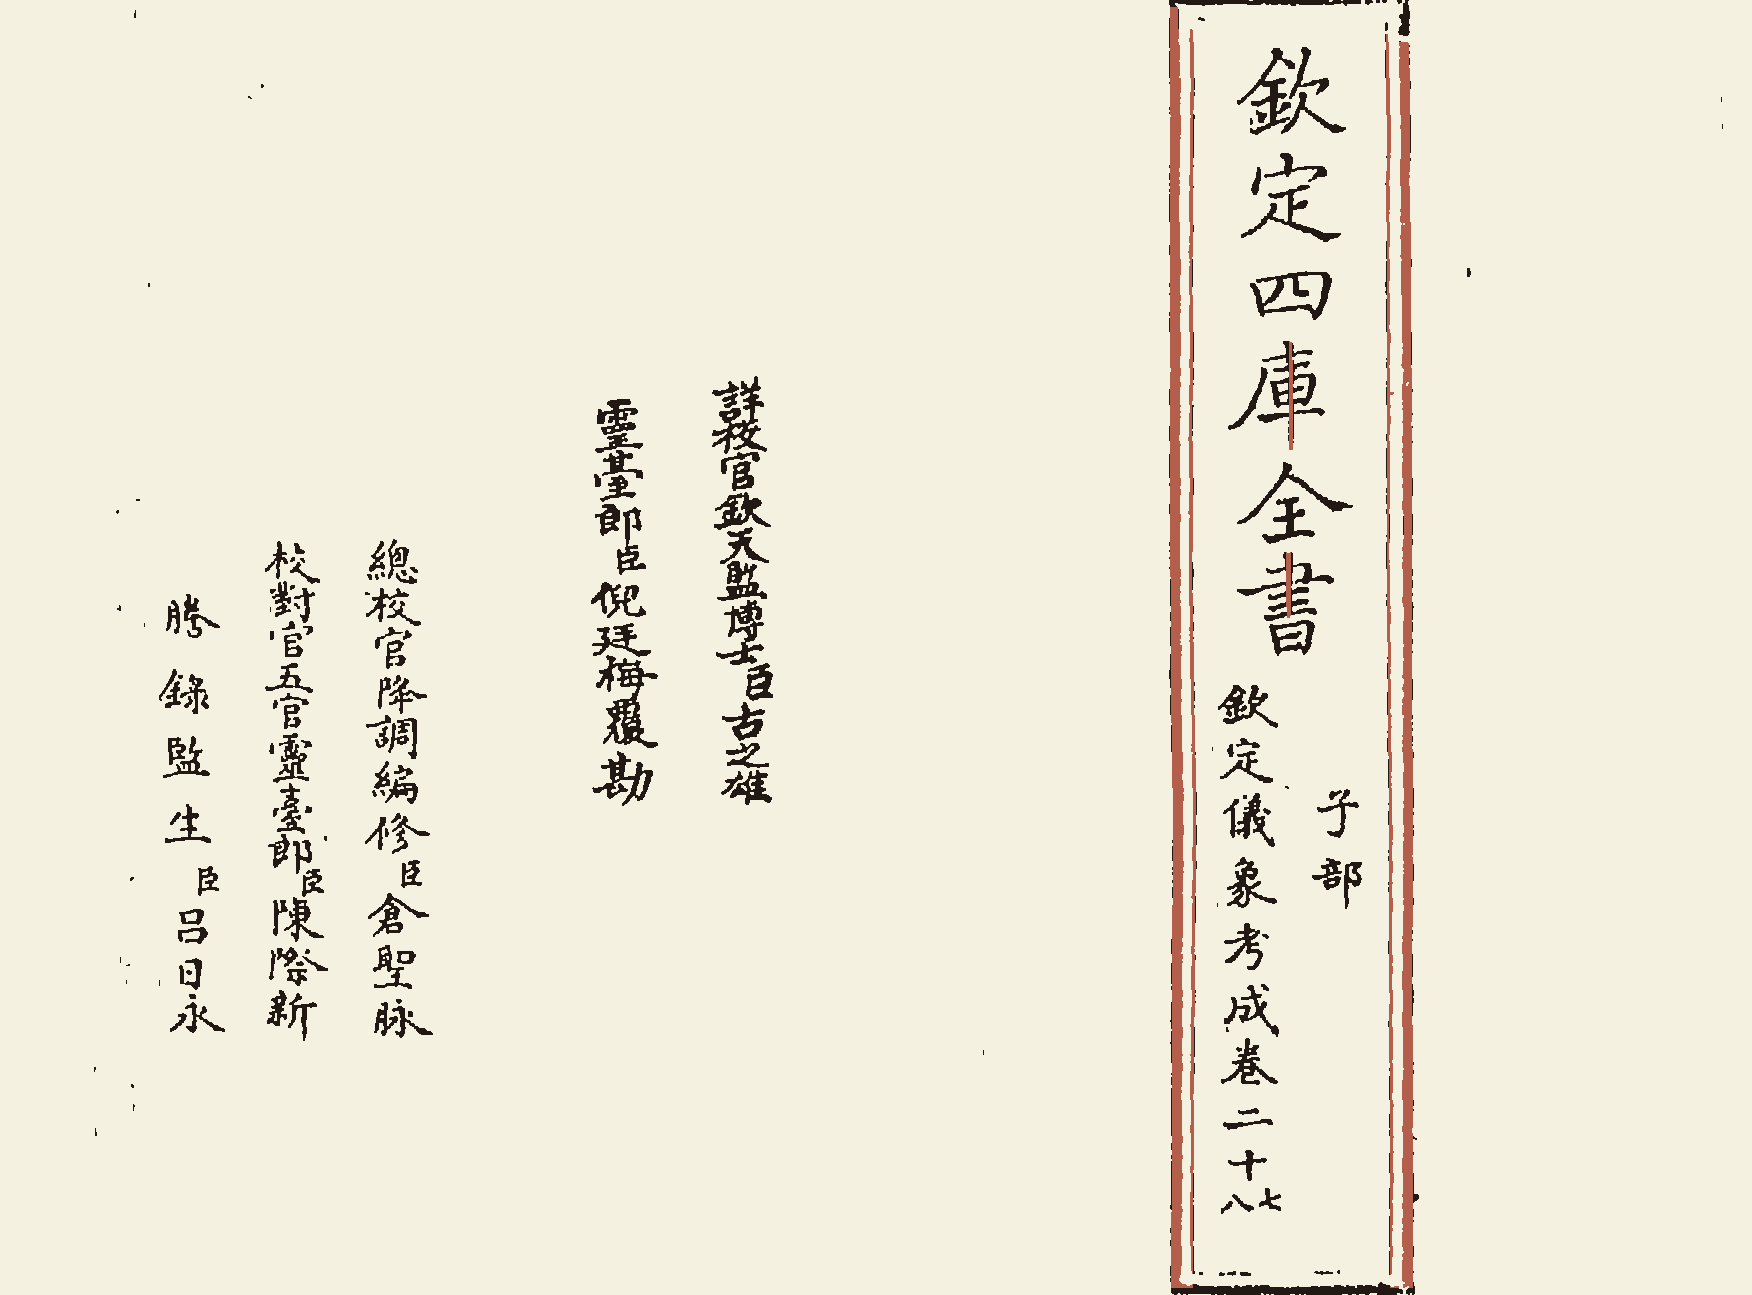
\includegraphics[width=\paperwidth,height=\paperheight,keepaspectratio]{img/1668.png}\clearpage
\begin{正文}
% ---- 册793 葉1669 ----
\SetPageNumber{1}
欽定四庫全書\换行
欽定儀象考成卷二十七\换行
　天漢經緯度表一\换行
　　黄道北天漢度\换行
\char"200B\relax\换行
\char"200B\relax\换行
\char"200B\relax\换行
\char"200B\relax\换行
\char"200B\relax\换行
\char"200B\relax\换行
\char"200B\relax\换行
\char"200B\relax\换行
\char"200B\relax\换行
\char"200B\relax\换行
\char"200B\relax\换行
\char"200B\relax
\par
% ---- 册793 葉1672 ----
　　天漢黄赤經緯度表\换行
晉書天文志云天漢起東方經箕尾之間謂之漢津乃\换行
分為二道其南經傳説魚天籥天弁河鼓其北經龜貫\换行
箕下次絡南斗魁左旗至天津下而合南道乃西南行\换行
又分夾瓠𤓰絡人星杵造父螣蛇王良附路閣道北端\换行
大陵天船卷舌而南行絡五車經北河之南入東井水\换行
位而東南行絡南河闕邱天狗天記天稷至七星南而\换行
没明史天文志云近年浮海之人至赤道以南見雲漢\换行
過天狗之墟抵天社海石之南踰南船帶海山貫十字\换行
\抬头[1]架蜜蜂傍馬腹經南門絡三角龜杵而屬扵尾宿是為帶\换行
\抬头[1]天一周靈䑓儀象志天漢經緯度分列黄道南北赤道南\换行
\抬头[1]北四表與明史合但不按宮次或分二界或分三界或分\换行
\抬头[1]四界逐度列表其分合曲折之處尚有未詳今亦分黄赤\换行
\抬头[1]南北四表而各按宮次分南界北界南之北界北之南界\换行
各列四層其分合既為明晰至其曲折之處經緯或有\换行
不同又扵每度之間細分列表按數圖之庶合懸象云
\par
\end{正文}\clearpage
\嵌图{146.56pt}{202.31pt}{838.64pt}{585.16pt}{img/1673.png}
\begin{正文}
% ---- 册793 葉1673 图版 ----
\SetPageNumber{3}
\插图页
\char"200B\relax\换行
\char"200B\relax\换行
\char"200B\relax\换行
\char"200B\relax\换行
\char"200B\relax\换行
\char"200B\relax\换行
\char"200B\relax\换行
\char"200B\relax\换行
\char"200B\relax\换行
\char"200B\relax\换行
\char"200B\relax\换行
\char"200B\relax\换行
\char"200B\relax\换行
\char"200B\relax\换行
\char"200B\relax\换行
\char"200B\relax
\恢复丝栏\par
\end{正文}\clearpage
\嵌图{144.59pt}{205.10pt}{842.59pt}{579.59pt}{img/1676.png}
\begin{正文}
% ---- 册793 葉1676 图版 ----
\SetPageNumber{4}
\插图页
\char"200B\relax\换行
\char"200B\relax\换行
\char"200B\relax\换行
\char"200B\relax\换行
\char"200B\relax\换行
\char"200B\relax\换行
\char"200B\relax\换行
\char"200B\relax\换行
\char"200B\relax\换行
\char"200B\relax\换行
\char"200B\relax\换行
\char"200B\relax\换行
\char"200B\relax\换行
\char"200B\relax\换行
\char"200B\relax\换行
\char"200B\relax
\恢复丝栏\par
\end{正文}\clearpage
\嵌图{150.52pt}{204.54pt}{830.72pt}{580.72pt}{img/1677.png}
\begin{正文}
% ---- 册793 葉1677 图版 ----
\SetPageNumber{5}
\插图页
\char"200B\relax\换行
\char"200B\relax\换行
\char"200B\relax\换行
\char"200B\relax\换行
\char"200B\relax\换行
\char"200B\relax\换行
\char"200B\relax\换行
\char"200B\relax\换行
\char"200B\relax\换行
\char"200B\relax\换行
\char"200B\relax\换行
\char"200B\relax\换行
\char"200B\relax\换行
\char"200B\relax\换行
\char"200B\relax\换行
\char"200B\relax
\恢复丝栏\par
\end{正文}\clearpage
\嵌图{146.62pt}{204.17pt}{838.53pt}{581.46pt}{img/1680.png}
\begin{正文}
% ---- 册793 葉1680 图版 ----
\SetPageNumber{6}
\插图页
\char"200B\relax\换行
\char"200B\relax\换行
\char"200B\relax\换行
\char"200B\relax\换行
\char"200B\relax\换行
\char"200B\relax\换行
\char"200B\relax\换行
\char"200B\relax\换行
\char"200B\relax\换行
\char"200B\relax\换行
\char"200B\relax\换行
\char"200B\relax\换行
\char"200B\relax\换行
\char"200B\relax\换行
\char"200B\relax\换行
\char"200B\relax
\恢复丝栏\par
\end{正文}\clearpage
\嵌图{144.63pt}{202.37pt}{842.50pt}{585.05pt}{img/1681.png}
\begin{正文}
% ---- 册793 葉1681 图版 ----
\SetPageNumber{7}
\插图页
\char"200B\relax\换行
\char"200B\relax\换行
\char"200B\relax\换行
\char"200B\relax\换行
\char"200B\relax\换行
\char"200B\relax\换行
\char"200B\relax\换行
\char"200B\relax\换行
\char"200B\relax\换行
\char"200B\relax\换行
\char"200B\relax\换行
\char"200B\relax\换行
\char"200B\relax\换行
\char"200B\relax\换行
\char"200B\relax\换行
\char"200B\relax
\恢复丝栏\par
\end{正文}\clearpage
\嵌图{146.56pt}{205.07pt}{838.64pt}{579.65pt}{img/1684.png}
\begin{正文}
% ---- 册793 葉1684 图版 ----
\SetPageNumber{8}
\插图页
\char"200B\relax\换行
\char"200B\relax\换行
\char"200B\relax\换行
\char"200B\relax\换行
\char"200B\relax\换行
\char"200B\relax\换行
\char"200B\relax\换行
\char"200B\relax\换行
\char"200B\relax\换行
\char"200B\relax\换行
\char"200B\relax\换行
\char"200B\relax\换行
\char"200B\relax\换行
\char"200B\relax\换行
\char"200B\relax\换行
\char"200B\relax
\恢复丝栏\par
\end{正文}\clearpage
\嵌图{146.56pt}{203.63pt}{838.64pt}{582.54pt}{img/1685.png}
\begin{正文}
% ---- 册793 葉1685 图版 ----
\SetPageNumber{9}
\插图页
\char"200B\relax\换行
\char"200B\relax\换行
\char"200B\relax\换行
\char"200B\relax\换行
\char"200B\relax\换行
\char"200B\relax\换行
\char"200B\relax\换行
\char"200B\relax\换行
\char"200B\relax\换行
\char"200B\relax\换行
\char"200B\relax\换行
\char"200B\relax\换行
\char"200B\relax\换行
\char"200B\relax\换行
\char"200B\relax\换行
\char"200B\relax
\恢复丝栏\par
\end{正文}\clearpage
\嵌图{146.62pt}{206.54pt}{838.53pt}{576.71pt}{img/1688.png}
\begin{正文}
% ---- 册793 葉1688 图版 ----
\SetPageNumber{10}
\插图页
\char"200B\relax\换行
\char"200B\relax\换行
\char"200B\relax\换行
\char"200B\relax\换行
\char"200B\relax\换行
\char"200B\relax\换行
\char"200B\relax\换行
\char"200B\relax\换行
\char"200B\relax\换行
\char"200B\relax\换行
\char"200B\relax\换行
\char"200B\relax\换行
\char"200B\relax\换行
\char"200B\relax\换行
\char"200B\relax\换行
\char"200B\relax
\恢复丝栏\par
\end{正文}\clearpage
\嵌图{146.62pt}{203.71pt}{838.53pt}{582.37pt}{img/1689.png}
\begin{正文}
% ---- 册793 葉1689 图版 ----
\SetPageNumber{11}
\插图页
\char"200B\relax\换行
\char"200B\relax\换行
\char"200B\relax\换行
\char"200B\relax\换行
\char"200B\relax\换行
\char"200B\relax\换行
\char"200B\relax\换行
\char"200B\relax\换行
\char"200B\relax\换行
\char"200B\relax\换行
\char"200B\relax\换行
\char"200B\relax\换行
\char"200B\relax\换行
\char"200B\relax\换行
\char"200B\relax\换行
\char"200B\relax
\恢复丝栏\par
\end{正文}\clearpage
\嵌图{144.68pt}{200.43pt}{842.41pt}{588.92pt}{img/1692.png}
\begin{正文}
% ---- 册793 葉1692 图版 ----
\SetPageNumber{12}
\插图页
\char"200B\relax\换行
\char"200B\relax\换行
\char"200B\relax\换行
\char"200B\relax\换行
\char"200B\relax\换行
\char"200B\relax\换行
\char"200B\relax\换行
\char"200B\relax\换行
\char"200B\relax\换行
\char"200B\relax\换行
\char"200B\relax\换行
\char"200B\relax\换行
\char"200B\relax\换行
\char"200B\relax\换行
\char"200B\relax\换行
\char"200B\relax
\恢复丝栏\par
\end{正文}\clearpage
\嵌图{146.67pt}{203.58pt}{838.42pt}{582.63pt}{img/1693.png}
\begin{正文}
% ---- 册793 葉1693 图版 ----
\SetPageNumber{13}
\插图页
\char"200B\relax\换行
\char"200B\relax\换行
\char"200B\relax\换行
\char"200B\relax\换行
\char"200B\relax\换行
\char"200B\relax\换行
\char"200B\relax\换行
\char"200B\relax\换行
\char"200B\relax\换行
\char"200B\relax\换行
\char"200B\relax\换行
\char"200B\relax\换行
\char"200B\relax\换行
\char"200B\relax\换行
\char"200B\relax\换行
\char"200B\relax
\恢复丝栏\par
\end{正文}\clearpage
\嵌图{148.48pt}{204.18pt}{834.81pt}{581.44pt}{img/1696.png}
\begin{正文}
% ---- 册793 葉1696 图版 ----
\SetPageNumber{14}
\插图页
\char"200B\relax\换行
\char"200B\relax\换行
\char"200B\relax\换行
\char"200B\relax\换行
\char"200B\relax\换行
\char"200B\relax\换行
\char"200B\relax\换行
\char"200B\relax\换行
\char"200B\relax\换行
\char"200B\relax\换行
\char"200B\relax\换行
\char"200B\relax\换行
\char"200B\relax\换行
\char"200B\relax\换行
\char"200B\relax\换行
\char"200B\relax
\恢复丝栏\par
\end{正文}\clearpage
\嵌图{148.48pt}{203.74pt}{834.81pt}{582.32pt}{img/1697.png}
\begin{正文}
% ---- 册793 葉1697 图版 ----
\SetPageNumber{15}
\插图页
\char"200B\relax\换行
\char"200B\relax\换行
\char"200B\relax\换行
\char"200B\relax\换行
\char"200B\relax\换行
\char"200B\relax\换行
\char"200B\relax\换行
\char"200B\relax\换行
\char"200B\relax\换行
\char"200B\relax\换行
\char"200B\relax\换行
\char"200B\relax\换行
\char"200B\relax\换行
\char"200B\relax\换行
\char"200B\relax\换行
\char"200B\relax
\恢复丝栏\par
\end{正文}\clearpage
\嵌图{145.44pt}{220.43pt}{591.34pt}{572.40pt}{img/1700.png}
\begin{正文}
% ---- 册793 葉1700 ----
\SetPageNumber{16}
\插图页
\char"200B\relax\换行
\char"200B\relax\换行
\char"200B\relax\换行
\char"200B\relax\换行
\char"200B\relax\换行
\char"200B\relax\换行
\char"200B\relax\换行
\char"200B\relax\换行
\恢复丝栏
\char"200B\relax\换行
\char"200B\relax\换行
\char"200B\relax\换行
\char"200B\relax\换行
\char"200B\relax\换行
\char"200B\relax\换行
欽定儀象考成卷二十七\换行
\char"200B\relax
\par

% ======== 卷二十八（8行21字）========
\par\end{正文}\clearpage
\chapter*{欽定儀象考成卷二十八}
\begin{正文}
% ---- 册793 葉1701 ----
\SetPageNumber{1}
欽定四庫全書\换行
欽定儀象考成卷二十八\换行
　天漢經緯度表二\换行
　　黄道南天漢度\换行
\char"200B\relax\换行
\char"200B\relax\换行
\char"200B\relax\换行
\char"200B\relax\换行
\char"200B\relax\换行
\char"200B\relax\换行
\char"200B\relax\换行
\char"200B\relax\换行
\char"200B\relax\换行
\char"200B\relax\换行
\char"200B\relax\换行
\char"200B\relax
\par
\end{正文}\clearpage
\嵌图{146.40pt}{205.08pt}{838.96pt}{579.63pt}{img/1704.png}
\begin{正文}
% ---- 册793 葉1704 图版 ----
\SetPageNumber{2}
\插图页
\char"200B\relax\换行
\char"200B\relax\换行
\char"200B\relax\换行
\char"200B\relax\换行
\char"200B\relax\换行
\char"200B\relax\换行
\char"200B\relax\换行
\char"200B\relax\换行
\char"200B\relax\换行
\char"200B\relax\换行
\char"200B\relax\换行
\char"200B\relax\换行
\char"200B\relax\换行
\char"200B\relax\换行
\char"200B\relax\换行
\char"200B\relax
\恢复丝栏\par
\end{正文}\clearpage
\嵌图{142.61pt}{203.77pt}{846.55pt}{582.24pt}{img/1705.png}
\begin{正文}
% ---- 册793 葉1705 图版 ----
\SetPageNumber{3}
\插图页
\char"200B\relax\换行
\char"200B\relax\换行
\char"200B\relax\换行
\char"200B\relax\换行
\char"200B\relax\换行
\char"200B\relax\换行
\char"200B\relax\换行
\char"200B\relax\换行
\char"200B\relax\换行
\char"200B\relax\换行
\char"200B\relax\换行
\char"200B\relax\换行
\char"200B\relax\换行
\char"200B\relax\换行
\char"200B\relax\换行
\char"200B\relax
\恢复丝栏\par
\end{正文}\clearpage
\嵌图{142.64pt}{202.79pt}{846.47pt}{584.21pt}{img/1708.png}
\begin{正文}
% ---- 册793 葉1708 图版 ----
\SetPageNumber{4}
\插图页
\char"200B\relax\换行
\char"200B\relax\换行
\char"200B\relax\换行
\char"200B\relax\换行
\char"200B\relax\换行
\char"200B\relax\换行
\char"200B\relax\换行
\char"200B\relax\换行
\char"200B\relax\换行
\char"200B\relax\换行
\char"200B\relax\换行
\char"200B\relax\换行
\char"200B\relax\换行
\char"200B\relax\换行
\char"200B\relax\换行
\char"200B\relax
\恢复丝栏\par
\end{正文}\clearpage
\嵌图{144.63pt}{201.77pt}{842.50pt}{586.25pt}{img/1709.png}
\begin{正文}
% ---- 册793 葉1709 图版 ----
\SetPageNumber{5}
\插图页
\char"200B\relax\换行
\char"200B\relax\换行
\char"200B\relax\换行
\char"200B\relax\换行
\char"200B\relax\换行
\char"200B\relax\换行
\char"200B\relax\换行
\char"200B\relax\换行
\char"200B\relax\换行
\char"200B\relax\换行
\char"200B\relax\换行
\char"200B\relax\换行
\char"200B\relax\换行
\char"200B\relax\换行
\char"200B\relax\换行
\char"200B\relax
\恢复丝栏\par
\end{正文}\clearpage
\嵌图{142.64pt}{207.02pt}{846.47pt}{575.75pt}{img/1712.png}
\begin{正文}
% ---- 册793 葉1712 图版 ----
\SetPageNumber{6}
\插图页
\char"200B\relax\换行
\char"200B\relax\换行
\char"200B\relax\换行
\char"200B\relax\换行
\char"200B\relax\换行
\char"200B\relax\换行
\char"200B\relax\换行
\char"200B\relax\换行
\char"200B\relax\换行
\char"200B\relax\换行
\char"200B\relax\换行
\char"200B\relax\换行
\char"200B\relax\换行
\char"200B\relax\换行
\char"200B\relax\换行
\char"200B\relax
\恢复丝栏\par
\end{正文}\clearpage
\嵌图{144.63pt}{205.22pt}{842.50pt}{579.36pt}{img/1713.png}
\begin{正文}
% ---- 册793 葉1713 图版 ----
\SetPageNumber{7}
\插图页
\char"200B\relax\换行
\char"200B\relax\换行
\char"200B\relax\换行
\char"200B\relax\换行
\char"200B\relax\换行
\char"200B\relax\换行
\char"200B\relax\换行
\char"200B\relax\换行
\char"200B\relax\换行
\char"200B\relax\换行
\char"200B\relax\换行
\char"200B\relax\换行
\char"200B\relax\换行
\char"200B\relax\换行
\char"200B\relax\换行
\char"200B\relax
\恢复丝栏\par
\end{正文}\clearpage
\嵌图{142.64pt}{203.74pt}{846.47pt}{582.32pt}{img/1716.png}
\begin{正文}
% ---- 册793 葉1716 图版 ----
\SetPageNumber{8}
\插图页
\char"200B\relax\换行
\char"200B\relax\换行
\char"200B\relax\换行
\char"200B\relax\换行
\char"200B\relax\换行
\char"200B\relax\换行
\char"200B\relax\换行
\char"200B\relax\换行
\char"200B\relax\换行
\char"200B\relax\换行
\char"200B\relax\换行
\char"200B\relax\换行
\char"200B\relax\换行
\char"200B\relax\换行
\char"200B\relax\换行
\char"200B\relax
\恢复丝栏\par
\end{正文}\clearpage
\嵌图{142.64pt}{205.52pt}{846.47pt}{578.76pt}{img/1717.png}
\begin{正文}
% ---- 册793 葉1717 图版 ----
\SetPageNumber{9}
\插图页
\char"200B\relax\换行
\char"200B\relax\换行
\char"200B\relax\换行
\char"200B\relax\换行
\char"200B\relax\换行
\char"200B\relax\换行
\char"200B\relax\换行
\char"200B\relax\换行
\char"200B\relax\换行
\char"200B\relax\换行
\char"200B\relax\换行
\char"200B\relax\换行
\char"200B\relax\换行
\char"200B\relax\换行
\char"200B\relax\换行
\char"200B\relax
\恢复丝栏\par
\end{正文}\clearpage
\嵌图{144.63pt}{200.98pt}{842.50pt}{587.83pt}{img/1720.png}
\begin{正文}
% ---- 册793 葉1720 图版 ----
\SetPageNumber{10}
\插图页
\char"200B\relax\换行
\char"200B\relax\换行
\char"200B\relax\换行
\char"200B\relax\换行
\char"200B\relax\换行
\char"200B\relax\换行
\char"200B\relax\换行
\char"200B\relax\换行
\char"200B\relax\换行
\char"200B\relax\换行
\char"200B\relax\换行
\char"200B\relax\换行
\char"200B\relax\换行
\char"200B\relax\换行
\char"200B\relax\换行
\char"200B\relax
\恢复丝栏\par
\end{正文}\clearpage
\嵌图{146.62pt}{202.38pt}{838.53pt}{585.03pt}{img/1721.png}
\begin{正文}
% ---- 册793 葉1721 图版 ----
\SetPageNumber{11}
\插图页
\char"200B\relax\换行
\char"200B\relax\换行
\char"200B\relax\换行
\char"200B\relax\换行
\char"200B\relax\换行
\char"200B\relax\换行
\char"200B\relax\换行
\char"200B\relax\换行
\char"200B\relax\换行
\char"200B\relax\换行
\char"200B\relax\换行
\char"200B\relax\换行
\char"200B\relax\换行
\char"200B\relax\换行
\char"200B\relax\换行
\char"200B\relax
\恢复丝栏\par
\end{正文}\clearpage
\嵌图{144.59pt}{203.31pt}{842.59pt}{583.17pt}{img/1724.png}
\begin{正文}
% ---- 册793 葉1724 图版 ----
\SetPageNumber{12}
\插图页
\char"200B\relax\换行
\char"200B\relax\换行
\char"200B\relax\换行
\char"200B\relax\换行
\char"200B\relax\换行
\char"200B\relax\换行
\char"200B\relax\换行
\char"200B\relax\换行
\char"200B\relax\换行
\char"200B\relax\换行
\char"200B\relax\换行
\char"200B\relax\换行
\char"200B\relax\换行
\char"200B\relax\换行
\char"200B\relax\换行
\char"200B\relax
\恢复丝栏\par
\end{正文}\clearpage
\嵌图{144.59pt}{202.31pt}{842.59pt}{585.16pt}{img/1725.png}
\begin{正文}
% ---- 册793 葉1725 图版 ----
\SetPageNumber{13}
\插图页
\char"200B\relax\换行
\char"200B\relax\换行
\char"200B\relax\换行
\char"200B\relax\换行
\char"200B\relax\换行
\char"200B\relax\换行
\char"200B\relax\换行
\char"200B\relax\换行
\char"200B\relax\换行
\char"200B\relax\换行
\char"200B\relax\换行
\char"200B\relax\换行
\char"200B\relax\换行
\char"200B\relax\换行
\char"200B\relax\换行
\char"200B\relax
\恢复丝栏\par
% ---- 册793 葉1728 ----
\char"200B\relax\换行
\char"200B\relax\换行
\char"200B\relax\换行
\char"200B\relax\换行
\char"200B\relax\换行
\char"200B\relax\换行
\char"200B\relax\换行
\char"200B\relax\换行
\char"200B\relax\换行
\char"200B\relax\换行
\char"200B\relax\换行
\char"200B\relax\换行
\char"200B\relax\换行
\char"200B\relax\换行
\char"200B\relax\换行
欽定儀象考成卷二十八
\par

\par\end{正文}\clearpage

  \input{parts/part16}
\fi
\end{document}
"
% 單冊能獨立排出，因為每冊都自 \clearpage 起、自帶 \SetPageNumber，而書的
% 基本格點（8 行 21 字）正是 ltc-guji 的預設；卷首下改 9 行 20 字又改回，
% 也都在同一冊之內。整本仍是逐冊 \input，各冊的頁面與單冊排出的逐葉相同。
\ifdefined\ltcPart
  \input{parts/part\ltcPart}
\else
  \begin{正文}

% ======== 御製儀象考成序（8行21字）========
\end{正文}
\chapter*{御製儀象考成序}
\begin{正文}
\end{正文}\clearpage

  % ======== 卷首上（8行21字）========
\chapter*{欽定儀象考成卷首上}
\begin{正文}
\end{正文}\clearpage
\thispagestyle{empty}\noindent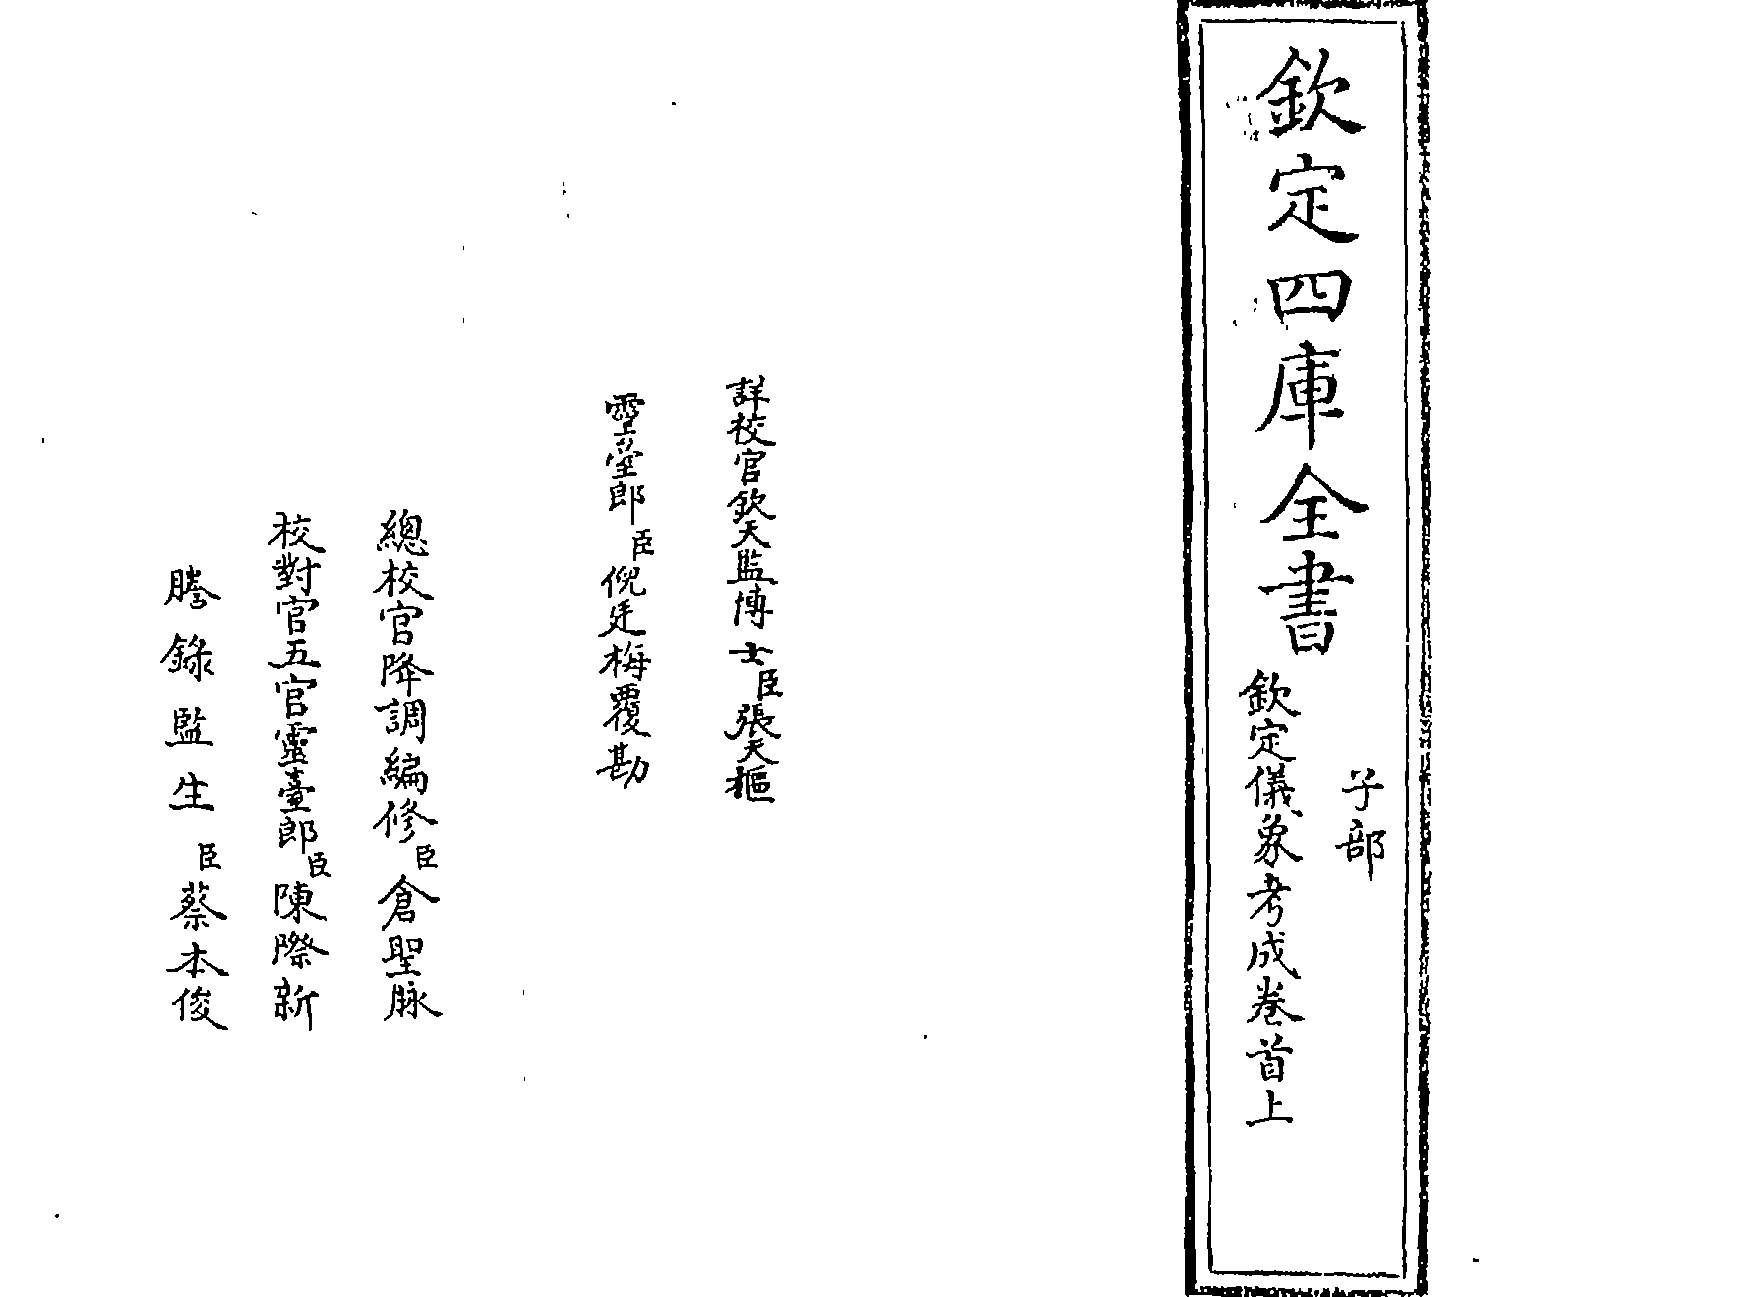
\includegraphics[width=\paperwidth,height=\paperheight,keepaspectratio]{img/0092.png}\clearpage
\begin{正文}
% ---- 册793 葉93 ----
\SetPageNumber{1}
欽定四庫全書\换行
欽定儀象考成卷首上\换行
御製璣衡撫辰儀説卷上\换行
　　儀制\换行
　　製法\换行
\char"200B\relax\换行
\char"200B\relax\换行
\char"200B\relax\换行
\char"200B\relax\换行
\char"200B\relax\换行
\char"200B\relax\换行
\char"200B\relax\换行
\char"200B\relax\换行
\char"200B\relax\换行
\char"200B\relax\换行
\char"200B\relax
\par
% ---- 册793 葉96 ----
御製璣衡撫辰儀説卷上之一\换行
　儀制\换行
　　全儀\换行
　　子午圏\换行
　　天常赤道\换行
　　赤極經圏\换行
　　遊旋赤道\换行
　　四遊圏\换行
　　指時度表\换行
　　借弧指時度表\换行
　　指緯度表\换行
　　立表\换行
　　平行立表\换行
　　平行借弧表\换行
　　綰經度表\换行
　　綰時度表
\par
% ---- 册793 葉97 ----
　　平行線測經度表\换行
\char"200B\relax\换行
\char"200B\relax\换行
\char"200B\relax\换行
\char"200B\relax\换行
\char"200B\relax\换行
\char"200B\relax\换行
\char"200B\relax\换行
\char"200B\relax\换行
\char"200B\relax\换行
\char"200B\relax\换行
\char"200B\relax\换行
\char"200B\relax\换行
\char"200B\relax\换行
\char"200B\relax\换行
\char"200B\relax
\par
\end{正文}\clearpage
\嵌图{153.00pt}{215.88pt}{395.02pt}{576.95pt}{img/0100.png}
\begin{正文}
% ---- 册793 葉100 ----
\SetPageNumber{4}
\插图页
\char"200B\relax\换行
\char"200B\relax\换行
\char"200B\relax\换行
\char"200B\relax\换行
\char"200B\relax\换行
\char"200B\relax\换行
\char"200B\relax\换行
\char"200B\relax\换行
\恢复丝栏
　　虞書舜典在璿璣玉衡以齊七政孔穎逹疏曰璣\换行
　　衡者王者正天文之器漢世以來謂之渾天儀者\换行
　　是也馬融云渾天儀可旋轉故曰璣衡其横簫所\换行
　　以視星宿也蔡邕云衡長八尺孔徑一寸下端望\换行
　　之以視星辰盖懸璣以象天而衡望之轉璣窺衡\换行
　　以知星宿是其説也上天之體不可得知測天之\换行
　　事見於經者惟此璿璣玉衡一事而已楊子法言\换行
　　云或問渾天曰落下閎營之鮮于妄人度之耿中
\par
% ---- 册793 葉101 ----
　　丞象之幾乎幾乎莫之能違也閎與妄人武帝時\换行
　　人宣帝時司農中丞耿夀昌始鑄銅為之象史官\换行
　　施用焉江南宋元嘉年太史丞錢樂\双列{\右小列{陳氏師凱曰}\左小列{錢樂本名樂}}\换行
　　\双列{\右小列{之孔疏}\左小列{脱之字}}鑄銅作渾天儀傳於齊梁周平江陵遷於\换行
　　長安尚書蔡註曰宋錢樂鑄銅作渾天儀衡長八\换行
　　尺孔徑一寸璣徑八尺圓周二丈五尺强轉而望\换行
　　之以知日月星辰之所在即璿璣玉衡之遺法也\换行
　　厯代以來其法漸密本朝因之為儀三重其在外\换行
　　者曰六合儀平置黒單環上刻十二辰八干四隅\换行
　　在地之位以凖地面而定四方側立黒雙環背刻\换行
　　去極度數以中分天脊直跨地平使其半入地下\换行
　　而結於其子午以為天經斜倚赤單環背刻赤道\换行
　　度數以平分天腹横繞天經亦使半出地上半入\换行
　　地下而結於其卯酉以為天緯三環表裏相結不\换行
　　動其天經之環則南北二極皆為圓軸虚中而内\换行
　　向以挈三辰四遊之環以其上下四方於是可考
\par
% ---- 册793 葉104 ----
　　故曰六合次其内曰三辰儀側立黒雙環亦刻去\换行
　　極度數外貫天經之軸内挈黄赤二道其赤道則\换行
　　為赤單環外依天緯亦刻宿度而結於黒雙環之\换行
　　卯酉其黄道則為黄單環亦刻宿度而又斜倚於\换行
　　赤道之腹以交結於卯酉而半入其内以為春分\换行
　　後之日軌半出其外以為秋分後之日軌又為白\换行
　　單環以承其交使不傾墊以其日月星辰於是可\换行
　　考故曰三辰其最在内者曰四遊儀亦為黒雙環\换行
　　如三辰儀之制以貫天經之軸其環之内則兩面\换行
　　當中各施直距外指兩軸而當其要中之内面又\换行
　　為小窽以受玉衡要中之小軸使衡既得隨環東\换行
　　西運轉又可隨處南北低昻以待占𠉀者之仰窺\换行
　　焉以其東西南北無不周徧故曰四遊此其法之\换行
　　大畧也今考前史漢初落下閎造渾天儀本無黄\换行
　　道或云賈逵所加或云李淳風所加或云一行所\换行
　　加而宋錢樂之渾儀之制雖有黄道並無黄道經
\par
% ---- 册793 葉105 ----
　　圈其四遊圈亦不貫於黄極則亦未盡黄道之用\换行
　　元郭守敬作簡儀乃分渾儀而變其制别設立運\换行
　　圏以測地平經緯度而不設黄道圏盖黄道與黄\换行
　　極經圏成經緯設黄道又設經圏則圏多而不便\换行
　　於測𠉀故不用黄道而專用赤道圈明正統三年\换行
　　　鑄銅渾儀簡儀於北京即宋元遺法也我\换行
　　朝康熙八年\换行
\抬头[1]聖祖仁皇帝命監臣南懐仁新製六儀赤道黄道分為二\换行
　　器皆不用地平圏而地平象限天體諸儀則地平\换行
　　之經緯與黄赤之錯綜皆已畢具康熙五十二年\换行
　　　又\换行
\抬头[1]命監臣紀利安製地平經緯儀合地平象限二儀而為一\换行
　　　其用尤便制作之妙於斯極矣我\换行
　皇上敬\换行
天法\换行
祖齊政勤民
\par
% ---- 册793 葉108 ----
親蒞靈臺徧觀儀象以渾天制最近古而時度信宜從\换行
　　今觀其㑹通斯成鉅典於是用今之數目合古之\换行
　　型模\换行
御製璣衡撫辰儀用裨測𠉀誠唐虞之遺意昭代之新\换行
　　規也儀制三重其在外者即古之六合儀而不用\换行
　　地平圏其正立雙環為子午圏兩面皆刻周天三\换行
　　百六十度自南北極起初度至中要九十度是為\换行
　　天經斜倚單環為天常赤道圏兩面皆刻周日十\换行
　　二時以子正午正當子午雙環中空之半而結於\换行
　　其中要是為天緯其南北二極皆設圓軸軸本實\换行
　　於子午雙環中空之間而軸内向以貫内二重之\换行
　　環其下承以雲座仰面正中開雙槽以受雙環東\换行
　　面正中開雲窩以受垂球下面置十字架施螺旋\换行
　　以取平架之東西兩端各植龍柱龍口銜珠開孔\换行
　　以承天常赤道卯酉之兩軸依觀象臺測定南北\换行
　　正線将座架安定則平面之四方正又依京師北
\par
% ---- 册793 葉109 ----
　　極出地三十九度五十五分自北極而上五十度\换行
　　五分即上應天頂自南極而下五十度五分即下\换行
　　對地心而應天頂之衝於天頂施小釘懸垂線而\换行
　　垂適當地心又適切於雙環之面不即不離則上\换行
　　下正立面之四方亦正而地平已在其中故不用\换行
　　地平圏也次其内即古之三辰儀而不用黄道圏\换行
　　其貫於二極之雙環為赤極經圏兩極各設軸孔\换行
　　以受天經之軸兩面皆刻周天三百六十度結於\换行
　　赤極經圏之中要與天常赤道平運者為遊旋赤\换行
　　道圈兩面皆刻周天三百六十度與天之赤道旋\换行
　　轉相應自經圏之南極作兩象限弧以承之使不\换行
　　傾墊測得三辰之赤道經緯度則黄道經緯可推\换行
　　且黄道與赤道之相距古逺今近縱或日久有差\换行
　　而儀器無庸改制故不用黄道圏也其在内者即\换行
　　古之四遊儀貫於二極之雙環為四遊圏兩面皆\换行
　　刻三百六十度定於遊圏之兩極者為直距綰於
\par
% ---- 册793 葉112 ----
　　直距之中心者為窺衡遊圏中要設直表以指經\换行
　　度及時窺衡右旁設直表以指緯度此古今所同\换行
　　無容置議者也是故體制倣乎渾天之舊而時度\换行
　　尤為整齊運量同於赤道新儀而重環更能合應\换行
　　至於借表窺測則上下左右無不宜焉夫羲和遺\换行
　　制不可考已漢世以來或作而不傳或傳而不久\换行
　　盖制器尚象若斯之難也而稽古宜今至我\换行
　朝乃臻盡善易繫傳云備物致用立成器以為天下\换行
　　利莫大乎聖人詎不信乎\换行
\char"200B\relax\换行
\char"200B\relax\换行
\char"200B\relax\换行
\char"200B\relax\换行
\char"200B\relax\换行
\char"200B\relax\换行
\char"200B\relax
\par
\end{正文}\clearpage
\嵌图{154.79pt}{220.57pt}{393.23pt}{572.26pt}{img/0118.png}
\begin{正文}
% ---- 册793 葉118 ----
\SetPageNumber{11}
\插图页
\char"200B\relax\换行
\char"200B\relax\换行
\char"200B\relax\换行
\char"200B\relax\换行
\char"200B\relax\换行
\char"200B\relax\换行
\char"200B\relax\换行
\char"200B\relax\换行
\恢复丝栏
子午圈所以正南北也天之南北定於兩極必先測定\换行
南北正線而後安置子午圈則子午圈即為南北之正\换行
線南北正而後日軌之髙下時刻之早晚中星之偏度\换行
可得而稽也其制雙環外徑六尺三寸内徑五尺六寸\换行
六分環面濶三寸二分厚九分中空一寸雙環之間四\换行
隅各施銅枕合而固之其中空之半為子午正線兩面\换行
各畫三百六十度每度六十分自南北極起初度至中\换行
要九十度古曰天經環西法舊曰緯圈盖織絲以直者
\par
% ---- 册793 葉122 ----
為經横者為緯古以其圈直立故曰經西法以其為横\换行
線所界之度故曰緯今按圈直而度横則其圈宜曰經\换行
圈而其度乃為緯度周禮賈公彦疏所謂南北之道謂\换行
之經元儒陳氏師凱所謂自北數向南去如機上數緯\换行
絲是也自兩極起初度者北極出地南極入地其度數\换行
皆自兩極起算也中要九十度者赤道為帯天之紘距\换行
兩極各一象限也南北極各設鋼軸軸本扁方長三寸\换行
濶二寸二分厚一寸實於隻環之間以鋼螺旋結之軸\换行
長六寸徑八分正當雙環中空之半内向以貫三辰四\换行
遊之環所以象天樞也\换行
\char"200B\relax\换行
\char"200B\relax\换行
\char"200B\relax\换行
\char"200B\relax\换行
\char"200B\relax\换行
\char"200B\relax
\par
\end{正文}\clearpage
\嵌图{148.32pt}{219.14pt}{399.70pt}{573.69pt}{img/0126.png}
\begin{正文}
% ---- 册793 葉126 ----
\SetPageNumber{13}
\插图页
\char"200B\relax\换行
\char"200B\relax\换行
\char"200B\relax\换行
\char"200B\relax\换行
\char"200B\relax\换行
\char"200B\relax\换行
\char"200B\relax\换行
\char"200B\relax\换行
\恢复丝栏
天常赤道所以正時刻也天左旋一日一周南北極持\换行
其兩端而赤道為其横帯以其常定不動故曰天常日\换行
循黄道右旋而其隨天西轉則係赤道之度日行臨於\换行
赤道之某位即為某時故時刻由赤道而正也其制單\换行
環外徑六尺一寸二分内徑五尺六寸四分環面濶二\换行
寸四分厚一寸四分平分其厚為赤道之中線兩面各\换行
畫周日十二時每時初正各四刻每刻十五分每一時\换行
當天之三十度每四刻當天之十五度每一分當天之
\par
% ---- 册793 葉130 ----
十五分以其子正午正線當子午雙環中空之半而結\换行
於其中要使其赤道中線適當子午圏之九十度兩圈\换行
相結成十字直角古曰天緯環西法舊曰赤道經圈盖\换行
古以其圈横運故曰緯西法以其為直線所界之度故\换行
曰經今按圈横而度直則其圈宜曰緯圈而其度乃為\换行
經度周禮賈公彦疏所謂東西之道謂之緯陳氏師凱\换行
所謂自東數向西去如機上數經絲是也上面午正時\换行
刻線結於子午圈之正北卯正居西酉正居東謂日影\换行
對照之時下面則子正居北午正居南卯正居東酉正\换行
居西為日行所臨之正位也\换行
\char"200B\relax\换行
\char"200B\relax\换行
\char"200B\relax\换行
\char"200B\relax\换行
\char"200B\relax\换行
\char"200B\relax
\par
\end{正文}\clearpage
\嵌图{153.38pt}{219.23pt}{394.64pt}{573.60pt}{img/0134.png}
\begin{正文}
% ---- 册793 葉134 ----
\SetPageNumber{15}
\插图页
\char"200B\relax\换行
\char"200B\relax\换行
\char"200B\relax\换行
\char"200B\relax\换行
\char"200B\relax\换行
\char"200B\relax\换行
\char"200B\relax\换行
\char"200B\relax\换行
\恢复丝栏
赤極經圏所以帯赤道也亦曰過極圏制如子午雙環\换行
在内而差小外徑五尺五寸六分内徑五尺一寸二分\换行
環面濶二寸二分厚八分中空一寸二分兩面皆畫三\换行
百六十度每度六十分一面自兩極起初度至赤道九\换行
十度以應天經一面自赤道起初度至兩極九十度以\换行
應赤緯南北極各設軸孔用扁方銅長三寸濶與環面\换行
等厚與雙環中空等中心開圓孔以受天經之軸其孔\换行
徑適容軸徑使旋轉不致動摇孔之兩面各施鋼片厚
\par
% ---- 册793 葉138 ----
四分使孔徑不致磨損兩軸孔之中徑適當雙環中空\换行
之半與兩極徑線參直以鋼螺旋結之環外南北極之\换行
兩端各施扁圓鋼子厚五分與内外兩雙環之分縫等\换行
貫於天經之軸使赤極經圈之中要九十度線適與子\换行
午圈之九十度相凖則内外兩圈上下四方俱合為一\换行
線而縱横經緯自宜悉協矣\换行
\char"200B\relax\换行
\char"200B\relax\换行
\char"200B\relax\换行
\char"200B\relax\换行
\char"200B\relax\换行
\char"200B\relax\换行
\char"200B\relax\换行
\char"200B\relax\换行
\char"200B\relax\换行
\char"200B\relax
\par
\end{正文}\clearpage
\嵌图{157.41pt}{218.38pt}{390.61pt}{574.45pt}{img/0142.png}
\begin{正文}
% ---- 册793 葉142 ----
\SetPageNumber{17}
\插图页
\char"200B\relax\换行
\char"200B\relax\换行
\char"200B\relax\换行
\char"200B\relax\换行
\char"200B\relax\换行
\char"200B\relax\换行
\char"200B\relax\换行
\char"200B\relax\换行
\恢复丝栏
遊旋赤道所以象天之運行而紀其赤道經度也制如\换行
天常赤道在内而差小外徑五尺五寸六分内徑五尺\换行
一寸二分環面濶二寸二分厚一寸二分平分其厚為\换行
赤道之中線兩面各畫周天三百六十度上面分為十\换行
二宫每宫三十度每度六十分下面自丑宫起初度右\换行
旋三百六十度以其丑宫未宫初度之線當赤經雙環\换行
中空之半而結於其中要使其赤道中線適當經圈之\换行
九十度兩圈相結成十字直角與天之赤道旋轉相應
\par
% ---- 册793 葉146 ----
又於經圏南極之兩旁設象限弧承於遊旋赤道辰宫\换行
戌宫之下以螺旋結之使不傾墊有天常赤道之不動\换行
者以定時又有遊旋赤道之常動者以紀度則赤道之\换行
逐宫逐度皆能周行於十二時而三辰之所躔與兩曜\换行
之相距皆可得而稽矣\换行
\char"200B\relax\换行
\char"200B\relax\换行
\char"200B\relax\换行
\char"200B\relax\换行
\char"200B\relax\换行
\char"200B\relax\换行
\char"200B\relax\换行
\char"200B\relax\换行
\char"200B\relax\换行
\char"200B\relax\换行
\char"200B\relax
\par
\end{正文}\clearpage
\嵌图{152.17pt}{219.82pt}{395.85pt}{573.01pt}{img/0150.png}
\begin{正文}
% ---- 册793 葉150 ----
\SetPageNumber{19}
\插图页
\char"200B\relax\换行
\char"200B\relax\换行
\char"200B\relax\换行
\char"200B\relax\换行
\char"200B\relax\换行
\char"200B\relax\换行
\char"200B\relax\换行
\char"200B\relax\换行
\恢复丝栏
四遊圈所以測三辰之赤道經緯度也制如赤經雙環\换行
在内而差小外徑五尺内徑四尺六寸八分環面濶一\换行
寸六分厚七分中空一寸四分盖三重雙環之外面皆\换行
相平而内重則漸薄中空則漸大取其輕重適宜亦便\换行
於設窺衡也兩面各畫三百六十度一面自北極起初\换行
度至南極一百八十度為去極度一面自赤道起初度\换行
至兩極各九十度為距緯度南北極各設軸孔以受夭\换行
經之軸與過極圈同環外南北極之兩端各施扁圓鋼
\par
% ---- 册793 葉152 ----
子厚六分與赤經四遊兩環之分縫等貫於天經之軸\换行
其下半周之中要安直表以指經度及時刻兩面對南\换行
北極各安直距如圓之通徑濶一寸六分厚七分中空\换行
一寸四分直距之二面對環之兩極作直徑線對環之\换行
九十度作横徑線十字相交中心開圓孔施螺旋小鋼\换行
軸而圓其末以綰窺衡窺衡長四尺七寸二分方一寸\换行
二分中空一寸上下兩端施方銅盖厚五分内三分方\换行
一寸入於管中外二分方一寸二分齊於管面中心開\换行
圓孔上端孔心留十字線以便測視管之四面亦各取\换行
中線上面安立表下端右面安指緯度表左右兩面之\换行
中心各開圓孔使直距中要小軸之末入其中以綰之\换行
則窺衡乃能南北低昂而隨雙環東西運轉焉窺衡連\换行
盖長四尺七寸六分比四遊環内徑長八分兩端各施\换行
鋼篐厚一分中要孔外施鋼眼錢亦厚一分使其左右\换行
適切於中空之内面上下兩端入於雙環内徑各四分\换行
則上下低昂自無偏側而所測經緯度必皆密合矣
\par
\end{正文}\clearpage
\嵌图{153.29pt}{217.38pt}{394.73pt}{575.45pt}{img/0153.png}
\begin{正文}
% ---- 册793 葉153 ----
\SetPageNumber{21}
\插图页
\char"200B\relax\换行
\char"200B\relax\换行
\char"200B\relax\换行
\char"200B\relax\换行
\char"200B\relax\换行
\char"200B\relax\换行
\char"200B\relax\换行
\char"200B\relax\换行
\恢复丝栏
指時度表通長七寸三分本長一寸六分形如方筒入\换行
於四遊雙環中空之間濶一寸四分與四遊環之中空\换行
等平分其濶即當窺衡之中線筒中施左右螺旋以充\换行
塞於中空之内使表不動移横帶長三寸二分濶五分\换行
兩端各鉤囬二分扣於環面之外表長五寸二分濶一\换行
寸其指時度之邊線對方筒之正中亦即窺衡之正中\换行
下端二寸四分厚三分切於遊旋赤道之面以指度分\换行
上端二寸八分厚二分切於天常赤道之面以指時刻
\par
% ---- 册793 葉156 ----
也\换行
\char"200B\relax\换行
\char"200B\relax\换行
\char"200B\relax\换行
\char"200B\relax\换行
\char"200B\relax\换行
\char"200B\relax\换行
\char"200B\relax\换行
\char"200B\relax\换行
\char"200B\relax\换行
\char"200B\relax\换行
\char"200B\relax\换行
\char"200B\relax\换行
\char"200B\relax\换行
\char"200B\relax\换行
\char"200B\relax
\par
\end{正文}\clearpage
\嵌图{151.20pt}{217.28pt}{396.82pt}{575.55pt}{img/0157.png}
\begin{正文}
% ---- 册793 葉157 ----
\SetPageNumber{23}
\插图页
\char"200B\relax\换行
\char"200B\relax\换行
\char"200B\relax\换行
\char"200B\relax\换行
\char"200B\relax\换行
\char"200B\relax\换行
\char"200B\relax\换行
\char"200B\relax\换行
\恢复丝栏
借弧指時度表其本方筒及横帶長濶並與前指時度\换行
表同横帶之下自左向右立安弧背一道長九寸三分\换行
濶一寸二分厚一分六釐弧背之末平安指時度表除\换行
弧背之厚長五寸二分濶一寸計自表本方筒之中線\换行
至指時度表之内邊長六寸七分當遊旋赤道之十五\换行
度當天常赤道之一小時測量時指時度表或為子午\换行
圏所礙則用此表視其所指之時度加四刻即為所測\换行
之時減十五度即為所測之度盖借弧指時度表在窺
\par
% ---- 册793 葉160 ----
衡之右所指雖視乎借表而所測則定於窺衡天常之\换行
時刻左旋故加三辰之度分右旋故減則用借弧指時\换行
度表察之與用指時度表等也\换行
\char"200B\relax\换行
\char"200B\relax\换行
\char"200B\relax\换行
\char"200B\relax\换行
\char"200B\relax\换行
\char"200B\relax\换行
\char"200B\relax\换行
\char"200B\relax\换行
\char"200B\relax\换行
\char"200B\relax\换行
\char"200B\relax\换行
\char"200B\relax\换行
\char"200B\relax
\par
\end{正文}\clearpage
\嵌图{151.20pt}{220.43pt}{396.82pt}{572.40pt}{img/0161.png}
\begin{正文}
% ---- 册793 葉161 ----
\SetPageNumber{25}
\插图页
\char"200B\relax\换行
\char"200B\relax\换行
\char"200B\relax\换行
\char"200B\relax\换行
\char"200B\relax\换行
\char"200B\relax\换行
\char"200B\relax\换行
\char"200B\relax\换行
\恢复丝栏
指緯度表其形兩曲安於窺衡下端之右面底長三寸\换行
濶九分平分其濶為中線對衡面中線以螺旋結之曲\换行
横七分與四遊環之厚等又曲長一寸七分切於四遊\换行
環之外面從中線減濶之半所以指緯度也\换行
\char"200B\relax\换行
\char"200B\relax\换行
\char"200B\relax\换行
\char"200B\relax
\par
\end{正文}\clearpage
\嵌图{153.29pt}{219.54pt}{394.73pt}{573.29pt}{img/0164.png}
\begin{正文}
% ---- 册793 葉164 ----
\SetPageNumber{26}
\插图页
\char"200B\relax\换行
\char"200B\relax\换行
\char"200B\relax\换行
\char"200B\relax\换行
\char"200B\relax\换行
\char"200B\relax\换行
\char"200B\relax\换行
\char"200B\relax\换行
\恢复丝栏
立表二座形直底平表髙底長各三寸二分濶九分厚\换行
一分平分其濶為中線表直立於底長之半與底面成\换行
直角距底面一寸一表向上開長方孔長一寸中留直\换行
線又上五分開圓孔徑四分中留十字線安於窺衡之\换行
上端一表依前度下開直縫上開小圓孔安於窺衡之\换行
下端各對衡面中線以螺旋結之測量時窺衡或為赤\换行
道及銅枕所礙則用此表盖兩表之孔心中線距衡面\换行
皆相等又與衡面之中線參直則用立表測之與用窺
\par
% ---- 册793 葉165 ----
衡等也\换行
\char"200B\relax\换行
\char"200B\relax\换行
\char"200B\relax\换行
\char"200B\relax\换行
\char"200B\relax\换行
\char"200B\relax\换行
\char"200B\relax\换行
\char"200B\relax\换行
\char"200B\relax\换行
\char"200B\relax\换行
\char"200B\relax\换行
\char"200B\relax\换行
\char"200B\relax\换行
\char"200B\relax\换行
\char"200B\relax
\par
\end{正文}\clearpage
\嵌图{153.00pt}{217.70pt}{395.02pt}{575.13pt}{img/0168.png}
\begin{正文}
% ---- 册793 葉168 ----
\SetPageNumber{28}
\插图页
\char"200B\relax\换行
\char"200B\relax\换行
\char"200B\relax\换行
\char"200B\relax\换行
\char"200B\relax\换行
\char"200B\relax\换行
\char"200B\relax\换行
\char"200B\relax\换行
\恢复丝栏
平行立表二座形曲底平底盤長四寸濶一寸二分厚\换行
一分中空長三寸二分濶九分與立表底盤之長濶等\换行
表曲如勾股股直如立表髙三寸二分濶九分勾横連\换行
於股末長五寸濶九分横植於底盤之末底盤中空冒\换行
於立表底盤之外以掐表固之測量時窺衡立表或為\换行
子午圏及龍柱所礙則用此表盖平行立表曲如勾股\换行
而與立表平行則用平行立表測之與用立表等亦與\换行
用窺衡等也
\par
\end{正文}\clearpage
\嵌图{153.00pt}{223.19pt}{395.02pt}{569.64pt}{img/0169.png}
\begin{正文}
% ---- 册793 葉169 ----
\SetPageNumber{29}
\插图页
\char"200B\relax\换行
\char"200B\relax\换行
\char"200B\relax\换行
\char"200B\relax\换行
\char"200B\relax\换行
\char"200B\relax\换行
\char"200B\relax\换行
\char"200B\relax\换行
\恢复丝栏
平行借弧表制如平行立表而倒正異盖四遊窺衡東\换行
西為子午圏及龍柱所礙南北為赤道及銅枕所礙則\换行
用平行立表猶是窺衡所能及而管孔被遮故其表平\换行
行正立即可見若近北極之星則東西既礙於子午圏\换行
南北又礙於極軸窺衡不能及自上測之不能及北極\换行
之南六度餘自下測之不能及北極之北六度餘故借\换行
十度作平行借弧表一表上植一表下垂則窺衡未及\换行
北極十度而窺孔之視線已與北極參直其法以半徑
\par
% ---- 册793 葉172 ----
一千萬為一率十度之正切線一百七十六萬三千二\换行
百七十為二率表之横勾距窺衡中心二尺三寸三分\换行
為三率求得四率四寸一分零八毫為表髙之中數\双列{\右小列{自}\左小列{窺}}\换行
\双列{\右小列{衡中線至直}\左小列{距中線之數}}上端之表立植於衡面則中數即表髙\双列{\右小列{中}\左小列{數}}\换行
\双列{\右小列{減衡方之半六分加表端距窺孔中心}\左小列{六分為表端至表本之髙仍與中數等}}下端之表自衡\换行
面下垂則於中數加衡方之半六分表端距窺孔中心\换行
六分又加平行横勾之濶九分得六寸二分零八毫為\换行
表之髙距表端下六分開圓孔又下五分開長方孔皆\换行
與立表制同凡測近北極之星測得距赤道北若干加\换行
十度即得星距赤道北之緯度若測赤道南之星亦可\换行
用此表但測得距赤道南若干減十度即得星距赤道\换行
南之緯度也\换行
\char"200B\relax\换行
\char"200B\relax\换行
\char"200B\relax\换行
\char"200B\relax
\par
\end{正文}\clearpage
\嵌图{155.09pt}{220.28pt}{392.93pt}{572.55pt}{img/0173.png}
\begin{正文}
% ---- 册793 葉173 ----
\SetPageNumber{31}
\插图页
\char"200B\relax\换行
\char"200B\relax\换行
\char"200B\relax\换行
\char"200B\relax\换行
\char"200B\relax\换行
\char"200B\relax\换行
\char"200B\relax\换行
\char"200B\relax\换行
\恢复丝栏
綰經度表通長四寸濶一寸四分平分其濶即當窺衡\换行
之中線其本方筒長一寸六分髙一寸八分入於四遊\换行
雙環之間以左右螺旋固之其末上下二面以夾遊旋\换行
赤道上面濶七分減本之半與窺衡中線參直下面以\换行
螺旋固之所以綰定遊旋赤道之經度於四遊圈也\换行
\char"200B\relax\换行
\char"200B\relax\换行
\char"200B\relax
\par
\end{正文}\clearpage
\嵌图{153.29pt}{222.42pt}{394.73pt}{570.41pt}{img/0176.png}
\begin{正文}
% ---- 册793 葉176 ----
\SetPageNumber{32}
\插图页
\char"200B\relax\换行
\char"200B\relax\换行
\char"200B\relax\换行
\char"200B\relax\换行
\char"200B\relax\换行
\char"200B\relax\换行
\char"200B\relax\换行
\char"200B\relax\换行
\恢复丝栏
綰時度表内外二截内截上下内三面綰於遊旋赤道\换行
之内規上面之末承於外截之下開二方孔以受外截\换行
之方足下面以螺旋固之外截上下外三面綰於天常\换行
赤道之外規上面之末覆於内截之上安二方足入於\换行
内截之方孔下面以螺旋固之凡以太陽時刻及經度\换行
測月星則内外截俱綰定别測月星若以經度求時刻\换行
則止綰定内截外截隨之運轉視其所當刻分即得時\换行
刻若以時刻求經度則止綰定外截任遊旋赤道之運
\par
% ---- 册793 葉177 ----
轉視其所當度分即得經度也\换行
\char"200B\relax\换行
\char"200B\relax\换行
\char"200B\relax\换行
\char"200B\relax\换行
\char"200B\relax\换行
\char"200B\relax\换行
\char"200B\relax\换行
\char"200B\relax\换行
\char"200B\relax\换行
\char"200B\relax\换行
\char"200B\relax\换行
\char"200B\relax\换行
\char"200B\relax\换行
\char"200B\relax\换行
\char"200B\relax
\par
\end{正文}\clearpage
\嵌图{146.46pt}{204.81pt}{838.85pt}{580.16pt}{img/0180.png}
\begin{正文}
% ---- 册793 葉180 图版 ----
\SetPageNumber{34}
\插图页
\char"200B\relax\换行
\char"200B\relax\换行
\char"200B\relax\换行
\char"200B\relax\换行
\char"200B\relax\换行
\char"200B\relax\换行
\char"200B\relax\换行
\char"200B\relax\换行
\char"200B\relax\换行
\char"200B\relax\换行
\char"200B\relax\换行
\char"200B\relax\换行
\char"200B\relax\换行
\char"200B\relax\换行
\char"200B\relax\换行
\char"200B\relax
\恢复丝栏\par
% ---- 册793 葉181 ----
平行線測經度表以赤經之平行線與直距之平行線\换行
相參直\双列{\右小列{赤經之平行線在圓周直距之平行線在}\左小列{圓心其平行線之間俱對南北極之中徑}}而測\换行
距星之經度也其制於直距南北極之兩端各安銅板\换行
如工字形正方二寸八分與直距二面之分等\双列{\右小列{直距二}\左小列{面各厚}}\换行
\双列{\右小列{七分中空一寸四}\左小列{分共二寸八分}}兩要各缺一長方長一寸六分濶七\换行
分與直距一面之分等\双列{\右小列{直距二面每面濶}\左小列{一寸六分厚七分}}扣於直距中\换行
空之間中心開圓孔貫於天經之軸四隅距中心一寸\换行
九分\双列{\右小列{銅板方二寸八分對角斜線三寸九分八釐四隅}\左小列{距中心各一寸九分九釐今取一寸九分餘九釐}}\换行
各安立柱圓頂開孔以穿直線與直距中徑平行下安\换行
小環以為結赤經平行線之用又按距星宫度於遊旋\换行
赤道安赤經平行線表其制上畫半圓内容半方自對\换行
角斜線起初度至横徑為四十五度其中直徑與指度\换行
表之邊線參直半圓中心安二遊表各長二寸距中心\换行
一寸九分邊留小臍中開小圓孔與直距四隅立柱之\换行
距中心等以線穿之上端繫於北極銅板對角之兩環\换行
下端貫於南極銅板對角之兩環各以垂球墜之乃視
\par
% ---- 册793 葉184 ----
四遊圏之所測與此平行線之所測相距若干度即将\换行
遊表對半圓度數安定下面以螺旋中徑以壓表固之\换行
此二線必與赤經中徑平行而與直距中徑之二平行\换行
線廣狹相等從左線視之與所測參直從右線視之亦\换行
與所測參直則此二線即為距星經度之凖線以此線\换行
對定距星将遊旋赤道隨之運轉又以四遊圏及窺管\换行
測日月及星即得其經緯度也盖以一星作距測日月\换行
及星必用兩測舊制黄道赤道二儀南北極之通徑皆\换行
係圓軸故測𠉀用通光耳實其正中與軸徑等兩邊各\换行
開直縫從左縫對軸左邊見光從右縫對軸右邊見光\换行
亦猶用平行線之意也今不用圓軸而用直距兩測相\换行
距有逺近則直距對角有斜横斜則二線平距之分狹\换行
横則二線平距之分廣\双列{\右小列{直鉅銅板方分也其對角斜分}\左小列{也二線平距則横分也對角斜}}\换行
\双列{\右小列{則平距為斜之方故狹對角}\左小列{横則平距為方之斜故廣}}其限自正斜起初度至四\换行
十五度而横四十五度以後復由横而斜至九十度與\换行
初度同\双列{\右小列{九十度以後復由斜而横至一百三十五度與}\左小列{四十五度同一百三十五度以後復由横而斜}}
\par
% ---- 册793 葉185 ----
\双列{\右小列{至一百八十度與初}\左小列{度同盈半周天而止}}如四遊環與平行線表同度是為\换行
初度是時直距對角正斜而其二線平距之分為斜之\换行
方此二線平距之最狹者也過此而四遊環距平行線\换行
表漸逺則直距對角漸横而二線平距漸廣至四遊環\换行
距平行線表四十五度則直距對角正横而其二線平\换行
距之分為方之斜此二線平距之最廣者也過此則直\换行
距對角又漸斜而二線平距又漸狹至九十度正斜而\换行
最狹故又與初度同也今欲使赤經平行線與直距平\换行
行線廣狹相等必以直距對角斜横之度合於赤道之\换行
半圓遊表二線距圓心各一寸九分通共三寸八分即\换行
直距銅板對角之斜分也半圓自内方之對角斜線起\换行
初度即直距對角之初度為正斜也半圓至横徑為四\换行
十五度即直距對角之四十五度為正横也設以二遊\换行
表通為一直表則與直距對角之斜横儼為一體但遊\换行
表在赤道若通為一直表則其線為赤道所礙而廣狹\换行
不靈且通為一表此端在横徑内彼端必在横徑外凡
\par
% ---- 册793 葉188 ----
斜線與十字線過心相交其彼端距横徑外之度與此\换行
端距横徑内之度必相等而距中徑之濶亦相等故以\换行
直表彼端當横徑外之度另用一遊表於横徑内按度\换行
安之其距中徑之濶必相等而與直距二平行線廣狹\换行
亦相等則用平行線表亦猶用通光耳之意也\换行
\char"200B\relax\换行
\char"200B\relax\换行
\char"200B\relax\换行
\char"200B\relax\换行
\char"200B\relax\换行
\char"200B\relax\换行
\char"200B\relax\换行
\char"200B\relax\换行
\char"200B\relax\换行
\char"200B\relax\换行
\char"200B\relax
\par
% ---- 册793 葉189 ----
御製璣衡撫辰儀説卷上之二\换行
　製法\换行
　　銅質宜精\换行
　　型制宜工\换行
　　鏇磨宜平\换行
　　取心宜中\换行
　　輕重宜審\换行
　　界度宜均\换行
　　兩徑合度\换行
　　合結均齊\换行
　　三重同心\换行
　　安置方正\换行
\char"200B\relax\换行
\char"200B\relax\换行
\char"200B\relax\换行
\char"200B\relax
\par
% ---- 册793 葉192 ----
　　銅質宜精\换行
凡鑄黄銅器具應用紅銅六成倭鉛四成鎔錬精到然\换行
後鑄之遼厯象志云古之鍊銅黒黄白青之氣盡然後\换行
用之故可施於久逺唐一行鑄渾天儀時稱精妙理固\换行
然也\换行
　　型制宜工\换行
凡鑄儀器以土為型必先治地極平外規較定制微大\换行
内規較定制微小其外環面如輪次内如輻次内如轂\换行
中留環心務極圓平合度則所鑄之體自亦圓平而鏇\换行
磨亦易為力矣\换行
　　鏇磨宜平\换行
凡製儀器必用鏇磨圓環中心當治方孔以受軸軸圓\换行
而方其端施於環心之方孔使環之上下前後左右不\换行
得動揺則鏇之自圓且平矣\换行
　　取心宜中\换行
凡製圓器必取中心心中則界正未鏇之前環心尚在
\par
% ---- 册793 葉193 ----
圓規方孔皆自環心取中逮鏇之既成則無中心矣而\换行
畫儀器之圓線則必先取中心為凖須以直木為環徑\换行
其兩端即如環之内規切𦂳安定約其中心嵌定鐵板\换行
任於環之内規取三處作點用三點求圓心法\双列{\右小列{法見數}\左小列{理精藴}}\换行
求得圓心即於鐵板作記次以鋼製規徑一規尖二規\换行
尖之本開方孔貫於規徑之兩端一尖安於圓心一尖\换行
按環面内外規之度各用螺旋固之於環之内外規旋\换行
轉比試處處皆當規面則圓心中矣次依環之内外規\换行
取外界圓線半徑之度安定規尖畫外界圓線為度之\换行
外界即以此半徑度将外界圓線分為六觚毎觚六十\换行
度\双列{\右小列{半徑與六十}\左小列{度之通弦等}}又取内界圓線半徑之度安定規尖畫\换行
内界圓線為度之内界自外界每觚六十度之點平分\换行
之得三十度各對中心作直線抵内界其過心對角之\换行
線即圓之通徑而平分環面為兩半周則圓界正矣次\换行
将直線輕微引出外界至外規用極方正矩度凖於側\换行
面單環則自側面即凖於彼面雙環則自此環之側面
\par
% ---- 册793 葉196 ----
凖於彼環之側面復自彼環之側面凖於彼環之彼面\换行
輕微畫線作記乃用前直木環徑切𦂳安定以縱横二\换行
線對於所凖之通徑果於中心相交則所凖確合否則\换行
又用前法取心務令得中單環即可如前畫彼面之圓\换行
線及十二度線雙環則俟審定輕重合釘枕銅再行比\换行
試確凖然後可畫彼面也\换行
　　輕重宜審\换行
凡環之兩半周輕重適均則平置無偏側之失運轉無\换行
游移之弊審量之法用圓直鐵鋌徑八分\双列{\右小列{與軸}\左小列{徑等}}長逾環\换行
徑平分中線卧置之使不動移而以環面之通徑線加\换行
於其上易置試之兩半周無有低昂則輕重適均否則\换行
非其線有微差即其體質不等細察磨治務得其輕重\换行
之適均則天常赤道之子正午正遊旋赤道之丑宫未\换行
宫三雙環之南北極皆以此通徑為凖乃将雙環已畫\换行
十二度線之一面置於下以通徑凖線四象分中安設\换行
銅枕以雙環彼面之通徑凖線合於上釘而固之復用
\par
% ---- 册793 葉197 ----
前法比試確凖取定中心然後畫内外界圓線及十二\换行
度線則兩面之圓心圓界允協矣\换行
　　界度宜均\换行
環心既中環界既正則界度可得而均矣顧諸環皆取\换行
度分惟天常赤道取時刻然時刻亦與度分相凖故取\换行
度分者将每觚六十度平分之得三十度又三分之各\换行
為十度自外界抵内界各畫直線而於内界之外畫圓\换行
線一層是為十度界次将每十度又十分之各為一度\换行
自外界抵十度界各畫直線而於十度界之外外界之\换行
内各畫圓線一層是為度界次於内度界之外外度界\换行
之内各畫圓線一層為十分界将每度六分之各為十\换行
分畫直線於其界内次於内外兩十分界之間畫圓線\换行
九道界為十層自每十分之初至每十分之末各作對\换行
角斜線則每一圓線與斜線之交即逐度之一分也取\换行
時刻者每三十度為一時平分之得十五度為一小時\换行
每一小時分為四刻自外界抵内界各畫直線而於内
\par
% ---- 册793 葉200 ----
界之外畫圓線一層是為時刻界次将每刻十五分三\换行
分之各為五分自外界抵時刻界各畫直線而於時刻\换行
界之外外界之内各畫圓線一層是為五分界次於内\换行
五分界之外外五分界之内又各畫圓線一層為一分\换行
界而将每五分又各五分之各為一分畫直線與其界\换行
内次於内外兩一分界之間畫圓線十一道界為十二\换行
層自每一分之初至每一分之末作對角斜線則每一\换行
圓線與斜線之交即逐分之五秒也\双列{\右小列{每分為六十秒十}\左小列{二分之故為五秒}}\换行
　　兩徑合度\换行
界度既均儀體正矣而其用尤在於軸稍滯則運轉不\换行
靈稍滑則游移不定是必軸身與軸孔兩徑相同密相\换行
合切而後無滯滑之失其法以極精鋼製成軸本軸身\换行
近本徑八分近末微細以銅製為軸孔\双列{\右小列{軸本軸孔皆扁}\左小列{方體詳前儀制}}\换行
\双列{\右小列{本}\左小列{篇}}上下孔面各嵌鋼片厚五分開成圓孔較軸身微小\换行
乃以油濡軸身轉而入之鋼屑如泥隨轉而出軸外孔\换行
内更不容間則以軸身治軸孔即以軸孔治軸身故兩
\par
% ---- 册793 葉201 ----
徑密相合切而自無滯滑之弊也\换行
　　合結均齊\换行
經緯各環製造既已如式而合結尤宜均齊其法先将\换行
子午圏之軸本過極圏四遊圏之軸孔三扁方治令方\换行
正十字分中\双列{\右小列{凡圏皆正立軸本軸孔入於雙環之間軸}\左小列{本扁方先将東西二面及南北兩端各對}}\换行
\双列{\右小列{軸徑取中線次将上面作十字線軸孔扁方先将上下}\左小列{二面各對軸孔作十字線次将東西二面南北兩端取}}\换行
\双列{\右小列{中}\左小列{線}}自中線各取雙環中空之半為其扁方之厚\双列{\右小列{子午圏}\左小列{中空一}}\换行
\双列{\右小列{寸過極圏中空一寸二分}\左小列{四遊圏中空一寸四分}}入於雙環中空之間\双列{\右小列{扁方微}\左小列{厚則不}}\换行
\双列{\右小列{動}\左小列{}}次於軸本軸孔之中心結通徑線\双列{\右小列{上下二軸各安銅}\左小列{管其端之中心開}}\换行
\双列{\右小列{小圓孔以線結之上下二孔各安}\左小列{銅片其中心開小圓孔以線結之}}雙環之中空二極之\换行
兩面各結十字線\双列{\右小列{雙環中空上下對扁方十字直線中}\左小列{間對銅枕厚分之半以線圍而結之}}\换行
\双列{\右小列{二極上下對扁方十字横線内}\左小列{面對極中徑以線圍而結之}}三線相參\双列{\右小列{通徑直線一}\左小列{十字圍線二}}\换行
\双列{\右小列{縱横}\左小列{皆三}}倘一線有毫釐之差則非中心有偏即十字線不\换行
正中心有偏者治扁方十字不正者治直線務令三線\换行
相合始為得中即於上下二扁方及四銅枕刻線作記\换行
以為合結之用乃将軸本軸孔之扁方二極雙環之兩
\par
% ---- 册793 葉204 ----
面皆自中線取分各作四孔以銅螺旋結之\夹注[only-column=right, auto-balance=false, grid-height=22.35pt, font-size=19.16pt]{徑三分試定}\夹注[only-column=left, auto-balance=false, grid-height=22.35pt, font-size=19.16pt]{易鋼螺旋徑}\换行
\抬头[1]\双列{\右小列{四}\左小列{分}}次將過極圏與遊旋赤道合結為三辰儀於過極雙環\换行
\抬头[1]之南北兩半周去極九十度中線之上下各取六分與九\换行
\抬头[1]十度作平行線自内規面向外各取一寸一分與南北極\换行
\抬头[1]作平行線依線裁成缺口以受赤道之内入又於遊旋赤\换行
\抬头[1]道之南北兩半周丑宮未宮之東或西取一寸四分與冬\换行
\抬头[1]夏至作平行線\双列{\右小列{作線於東則半弧背自西裁作線}\左小列{於西則半弧背自東裁法理皆同}}自外規\换行
\抬头[1]面向内各取一寸一分與辰宮戌宮作平行線依線裁去\换行
\抬头[1]半弧背\双列{\右小列{凡裁弧皆梢留有餘}\左小列{比試合切使令方正}}以足過極圏之内容則遊旋\换行
\抬头[1]赤道適容入於過極雙環之内而丑宮未宮線適當雙環\换行
中空之間\夹注[only-column=right, auto-balance=false, grid-height=23.75pt, font-size=20.36pt]{遊旋赤道外徑五尺五寸六分南北各裁一寸一分}\夹注[only-column=left, auto-balance=false, grid-height=23.75pt, font-size=20.36pt]{餘五尺三寸四分過極圏内徑五尺一寸二分}\换行
\夹注[only-column=right, auto-balance=false, grid-height=26.68pt, font-size=22.87pt]{南北各開一寸一分亦得五尺三寸四分九十度中線之}\夹注[only-column=left, auto-balance=false, grid-height=26.68pt, font-size=22.87pt]{上下各去六分共去一寸二分與遊旋赤道之厚等丑宮}\换行
\夹注[only-column=right, auto-balance=false, grid-height=26.68pt, font-size=22.87pt]{未宮之東或西去一寸四分為雙環厚分之半故遊旋赤}\夹注[only-column=left, auto-balance=false, grid-height=26.68pt, font-size=22.87pt]{道適容入於過極雙環之内而丑宮未宮線正當雙環中}\换行
\抬头[1]\双列{\右小列{空之}\左小列{間}}乃依裁去弧背之度除雙環分位另製弧背銅補全\换行
遊旋赤道\双列{\右小列{以銅釘}\左小列{固之}}並補畵度分仍将補銅拆去合結兩\换行
環使丑宮未宮正與所記中線相對又依前法於軸孔
\par
% ---- 册793 葉205 ----
結通徑線又自雙環上下扁方直線過丑宫未宫自扁\换行
方横線過辰宫戌宫結十字線三線相參合為一線復\换行
用半徑之斜度作尺製斜尖二管貫於尺之兩端斜度\换行
之一尖直指於南北極之外界一尖直指於辰宫戌宫\换行
之外界以螺旋固之轉相比試四象限皆相符合乃将\换行
補銅釘而固之又以遊旋赤道結於過極圏之兩要恐\换行
東西兩半周日久傾墊故製二象限弧以承其下其方\换行
一寸其弧即用過極圏一象限弧之度一端減雙環厚\换行
分之半一寸四分抵於過極圏南極之外面一端減赤\换行
道厚分之半六分承於遊旋赤道辰宫戌宫之下面外\换行
加二足各長一寸二分與環面之濶等以螺旋結之復\换行
以前尺斜度之兩象限仍相符合\双列{\右小列{南極有二弧不可量}\左小列{故惟量北極兩象限}}\换行
\双列{\右小列{此兩象限合則彼}\左小列{兩象限亦必合矣}}則遊旋赤道與過極圏相交成直角\换行
均齊方正而無有偏側矣次於三辰儀之外将子午圏\换行
與天常赤道合結為六合儀其子午雙環之南北兩半\换行
周去極九十度中線之上下裁成缺口天常赤道之南
\par
% ---- 册793 葉208 ----
北兩半周裁去半弧背並另製弧背銅補畫時刻皆與\换行
三辰儀同\双列{\右小列{子午圏内規面裁去一寸二分九十度上下}\左小列{各裁七分乃能容天常赤道數雖小異而其}}\换行
\双列{\右小列{理其法}\左小列{則同也}}乃立置天常赤道圏\双列{\右小列{中線左右以木承之}\左小列{使其下可結十字線}}以裁\换行
去半弧背之半周仰於上納入三辰儀\双列{\右小列{天常赤道順列}\左小列{之十二時與遊}}\换行
\双列{\右小列{旋赤道之十二宫同在一}\左小列{面乃向北極之上面也}}将子午圏合結於其外以木\换行
橙承其四隅使二環之面相平二極之線參直周圍之\换行
分縫皆相等天常遊旋二赤道下半周之分縫以木片\换行
實之使周圍亦相等乃将軸本入於子午圏南北極中\换行
空之間貫於過極圈南北極之軸孔使扁方之四孔與\换行
環面之四孔相合以銅螺旋結之依前法於軸端結通\换行
徑線子午卯酉各結十字線三線相參合為一線又用\换行
斜尺絜度四象限皆相符合乃将補銅釘而固之則子\换行
午圏與天常赤道相交成直角均齊方正無有偏側又\换行
卯正酉正有二小軸承於龍柱之珠孔自不虞傾墊矣\换行
至於四遊圏與窺衡合結為四遊儀其法較易已詳儀\换行
制並見後篇
\par
% ---- 册793 葉209 ----
　　三重同心\换行
前篇分言合結之法先正其樞心次正其經緯宜其無\换行
不正矣然三重合為一儀必三重同心施之測量乃得\换行
允協且以一重而言三線相參視之猶逺二線相切即\换行
有一線之差再以二重合之尤易參錯則先合定外二\换行
重比較確凖而後加入内一重其中正較為易得也盖\换行
子午圏過極圏貫於一軸則子午圈之軸本即天常赤\换行
道之中心過極圏之軸孔即遊旋赤道之中心如兩心\换行
皆得其中則兩心合而為一遊旋赤道之宫度線必與\换行
天常赤道之時刻線相合如一心有偏則兩心岐而為\换行
二而宫度線與時刻線不合矣然有偏東西與偏南北\换行
之殊又有軸本偏與軸孔偏之異偏東西者軸本軸孔\换行
厚分之中線不正當中空之半或偏東或偏西故丑宫\换行
未宫線亦偏子正午正之或東或西也偏南北者軸本\换行
軸孔扁方之中線不正當環面之徑或偏北或偏南故\换行
辰宫戌宫線亦偏卯正酉正之或北或南也治之之法
\par
% ---- 册793 葉212 ----
先正東西立置子午圏按方位安定北極在上南極在\换行
下午正在北子正在南卯正在西酉正在東\双列{\右小列{假如先是}\左小列{立置天常}}\换行
\双列{\右小列{赤道圏西面午正在北子正在南卯正在下酉正在上}\左小列{則子午圏西首為北極東首為南極乃以氊鋪地将天}}\换行
\双列{\右小列{常赤道圏向南推轉至子午圏在下即将子午圏東首}\左小列{轉北西首轉南向北推轉使北極在上則按位安定矣}}\换行
設以丑宫對於午正而未宫即對於子正轉以未宫對\换行
於午正而丑宫亦對於子正則東西正一有不對則東\换行
西偏比試兩次而軸本軸孔之偏正乃得而見焉凡兩\换行
試俱偏東俱偏西而偏分相等者為軸孔正軸本偏\双列{\右小列{軸}\左小列{孔}}\换行
\双列{\右小列{正則丑宫未宮線正當軸孔中心軸本偏東則挈之而}\左小列{東軸本偏西則挈之而西故所偏同向而偏分相等也}}\换行
東為軸本偏東西為軸本偏西其偏為偏分之一半\双列{\右小列{所}\左小列{謂}}\换行
\双列{\右小列{偏分者乃丑宫對午正未宫偏子正東西斜線之偏軸}\左小列{本軸孔所偏者乃丑宫未宮與子正午正平行線之偏}}\换行
\双列{\右小列{如丑宫對於午正未宫偏子正東二分若以丑宫未宫}\左小列{線與子正午正線平行則丑宫偏午正東一分未宫亦}}\换行
\双列{\右小列{偏子正東一分故其}\左小列{偏為偏分之一半}}其度之一分為尺之八毫\双列{\右小列{凡偏分}\左小列{皆以遊}}\换行
\双列{\右小列{旋赤道之度分而言遊旋赤道外徑五尺五寸六分周}\左小列{一丈七尺四寸六分七釐有竒以周天三百六十度每}}\换行
\双列{\右小列{度六十分除之得每分}\左小列{為八毫零八忽有竒}}偏東二分者為軸本偏東一分\换行
應向西移一分将上下軸本二扁方之東西記定\双列{\右小列{凡記}\左小列{方向}}
\par
% ---- 册793 葉213 ----
\双列{\右小列{只記一}\左小列{字可定}}西面去八毫東面加八毫\双列{\右小列{以薄銅}\左小列{葉釘之}}則軸本正而\换行
不偏矣偏西者凖此\双列{\右小列{凡治軸本軸孔應移八毫者上下}\左小列{各移八毫合之用線比較如上正}}\换行
\双列{\右小列{下偏則上之扁方不動下之扁方移一釐六毫如上亦}\左小列{微偏則上移四毫下移一釐二毫或上移六毫下移一}}\换行
\双列{\右小列{釐總使上下共移一釐六毫而其十字中心正}\左小列{移八毫上偏下正及偏南偏北者皆倣此治之}}凡兩試\换行
一偏東一偏西而偏分相等者為軸本正軸孔偏\双列{\右小列{軸本}\左小列{正則}}\换行
\双列{\右小列{子正午正線正當軸本中心設軸孔偏於戌宫之一面}\左小列{丑宫在北戌宫在西是軸孔偏於丑宫未宫線之西挈}}\换行
\双列{\右小列{之於軸本則丑宫未宫線必偏於子正午正線之東轉}\左小列{而丑宫在南戌宫在東是軸孔偏於丑宫未宫線之東}}\换行
\双列{\右小列{挈之於軸本則丑宫未宫線必偏於子正午}\左小列{正線之西故所偏異向而偏分亦相等也}}東為軸孔\换行
偏西西為軸孔偏東其偏亦為偏分之一半偏東二分\换行
者為軸孔偏西一分應向東移一分将上下軸孔二扁\换行
方及環面之東西記定\双列{\右小列{子午圏有定向故不須記}\左小列{過極圏有轉易故并記之}}東面\换行
去八毫西面加八毫則軸孔正而不偏矣偏西者凖此\换行
凡兩試俱偏東俱偏西而偏分不等者為軸本偏軸孔\换行
亦偏偏東分多為軸孔偏西偏西分多為軸孔偏東\双列{\右小列{軸}\左小列{本}}\换行
\双列{\右小列{偏東而軸孔又偏西挈之於軸本則丑宫未宫線必益}\左小列{在子正午正線之東故偏東分多也軸本偏西而軸孔}}\换行
\双列{\右小列{又偏東挈之於軸本則丑宫未宫線必}\左小列{益在子平午正線之西故偏西分多也}}其軸孔之偏為
\par
% ---- 册793 葉216 ----
偏多一半之半偏東多二分者為軸孔偏西半分偏西\换行
多二分者為軸孔偏東半分先治軸孔則偏分等\双列{\右小列{平行}\左小列{線之}}\换行
\双列{\右小列{偏既為偏分之一半而軸本軸孔在偏多之偏又為平}\左小列{行線所偏之一半故為一半之半如丑宫對於午正未}}\换行
\双列{\右小列{宫偏子正東二分未宫對於午正丑宫偏子正東四分}\左小列{是未宫在北偏東多二分若以丑宫未宫線與子正午}}\换行
\双列{\右小列{正線平行丑宫偏午正東一分則未宫亦偏子正東一}\左小列{分未宫偏午正東二分則丑宫亦偏子正東二分是未}}\换行
\双列{\右小列{宫在北偏東僅多一分均分其半将軸孔向東移半分}\左小列{則未宫在北丑宫未宫線偏子正午正東一分半丑宫}}\换行
\双列{\右小列{在北未宫在南丑宫未宫線亦偏子正午正東一分半}\左小列{試以丑宫對於午正則未宫偏子正東三分轉以未宮}}\换行
\双列{\右小列{對於午正丑宫亦偏子}\左小列{正東三分其偏分等}}東為軸本偏東西為軸本偏西\换行
其偏為偏分之一半再治軸本則不偏矣凡兩試一偏\换行
東一偏西而偏分不等者為軸孔偏軸本亦偏偏東分\换行
多為軸本偏東偏西分多為軸本偏西其軸本之偏亦\换行
為偏多一半之半偏東多二分者為軸本偏東半分偏\换行
西多二分者為軸本偏西半分先治軸本則偏分等\双列{\右小列{如}\左小列{丑}}\换行
\双列{\右小列{宫對於午正未宫偏子正東二分未宫對於午正丑宫}\左小列{偏子正西四分是未宫在北偏西多二分若以丑宫未}}\换行
\双列{\右小列{宫線與子正午正線平行丑宫偏午正東一分則未宫}\左小列{亦偏子正東一分未宫偏午正西二分則丑宫亦偏子}}\换行
\双列{\右小列{正西二分是未宫在北偏西僅多一分均分其半将軸}\左小列{本向東移半分則未宫在北丑宫未宫線偏子正午正}}
\par
% ---- 册793 葉217 ----
\双列{\右小列{西一分半丑宫在北未宫在南丑宫未宫線偏子正午}\左小列{正東亦一分半試以丑宫對於午正則未宫偏子正東}}\换行
\双列{\右小列{三分轉以未宫對於午正則丑}\左小列{宫偏子正西三分其偏分等}}東為軸孔偏西西為軸\换行
孔偏東其偏為偏分之一半再治軸孔則不偏矣凡兩\换行
試一正一偏者為軸本與軸孔之偏分相等一正一偏\换行
東者為軸本偏東軸孔偏西一正一偏西者為軸本偏\换行
西軸孔偏東其偏各為偏分一半之半\双列{\右小列{軸本偏東則子}\左小列{正午正線在軸}}\换行
\双列{\右小列{本之西若軸孔亦偏東其偏分等則丑宫未宫線必與}\左小列{子正午正線相合及其轉而之西則軸孔為偏西而丑}}\换行
\双列{\右小列{宫未宫線在軸孔之東挈之於軸本盖在子正午正線}\左小列{之東其偏必倍故半之為相等之偏又半之為平行線}}\换行
\双列{\右小列{之偏軸本偏}\左小列{西者凖此}}先治軸孔則變為俱偏東俱偏西其偏分\换行
等再治軸本則不偏矣若先治軸本則變為一偏東一\换行
偏西其偏分亦等再治軸孔則亦不偏矣以上凡治軸\换行
本軸孔之偏東偏西先并環面之東西記定平置子午\换行
圏用木橙承穏解螺旋下之磨治合度復結螺旋立置\换行
比試皆合則東西正其南北亦正者則辰宫戌宫與卯\换行
正酉正合為一線其南北不正者辰宫戌宫線亦必與\换行
卯正酉正線平行乃察其南北依前法以丑宫對於午
\par
% ---- 册793 葉220 ----
正未宫對於子正察辰宫戌宫線偏卯正酉正南北幾\换行
分轉以未宫對於午正丑宫對於子正察辰宫戌宫線\换行
偏卯正酉正南北幾分如此比試兩次則軸本軸孔之\换行
偏南偏北亦可得而見焉凡兩試俱偏南俱偏北而偏\换行
分相等者為軸本正軸孔偏南為軸本偏南北為軸夲\换行
偏北\双列{\右小列{皆與前法同理但}\左小列{易東西為南北耳}}偏南一分者為軸本偏南一分\换行
\双列{\右小列{辰宫戌宫線既與卯正酉正線}\左小列{平行故其偏分即為軸本之偏}}應向北移一分将上下\换行
軸本二扁方之南北記定環面四小孔向北開八毫軸\换行
夲扁方四小孔向南開八毫治令圓正易螺旋結之\双列{\右小列{環}\左小列{面}}\换行
\双列{\右小列{四小孔向北開八毫軸夲固可向北移矣然孔不圓正}\左小列{故将軸夲扁方四小孔向南開八毫治令圓正其徑較}}\换行
\双列{\右小列{大故易微大之銅螺旋結之至}\左小列{比試確凖乃易用鋼螺旋也}}則軸夲正而不偏矣偏\换行
北者凖此凡兩試一偏南一偏北而偏分相等者為軸\换行
本正軸孔偏偏南一分者為軸孔偏北一分應向南移\换行
一分将上下軸孔二扁方及環面之南北記定環面四\换行
小孔向南開八毫軸孔扁方四小孔向北開八毫治令\换行
圓正易螺旋結之則軸孔正而不偏矣偏北者凖此凡
\par
% ---- 册793 葉221 ----
兩試俱偏南俱偏北而偏分不等者為軸本偏軸孔亦\换行
偏偏南分多為軸孔偏北偏北分多為軸孔偏南其軸\换行
孔之偏為偏多之一半偏南多二分者為軸孔偏北一\换行
分偏北多二分者為軸孔偏南一分先治軸孔則偏分\换行
等\双列{\右小列{辰宫戌宫線既與卯正酉正線平行則軸本軸孔在}\左小列{偏多之偏止為平行線所偏之一半如丑宫對於午}}\换行
\双列{\右小列{正辰宫戌宫線偏卯正酉正南二分轉以未宫對於午}\左小列{正辰宫戌宫線偏卯正酉正南四分未宫在北偏南多}}\换行
\双列{\右小列{二分是軸孔偏於未宫一分将軸孔向丑宫移一分則}\左小列{丑宫在北辰宫戌宫線偏卯正酉正南三分未宫在北}}\换行
\双列{\右小列{辰宫戌宫線偏卯正酉}\左小列{正南亦三分其偏分等}}南為軸本偏南北為軸本偏北\换行
其偏即偏分再治軸本則不偏矣凡兩試一偏南一偏\换行
北而偏分不等者為軸孔偏軸本亦偏偏南分多為軸\换行
本偏南偏北分多為軸本偏北其軸本之偏亦為偏多\换行
之一半偏南多二分者為軸本偏南一分偏北多二分\换行
者為軸本偏北一分先治軸本則偏分等南為軸孔偏\换行
北北為軸孔偏南其偏即偏分再治軸孔則不偏矣凡\换行
兩試一正一偏者為軸本與軸孔之偏分相等一正一\换行
偏南者為軸本偏南軸孔偏北一正一偏北者為軸本
\par
% ---- 册793 葉224 ----
偏北軸孔偏南其偏各為偏分之一半先治軸孔則變\换行
為俱偏北俱偏南其偏分等再治軸本則不偏矣若先\换行
治軸本則變為一偏北一偏南其偏分亦等再治軸孔\换行
則亦不偏矣以上凡治軸本軸孔之偏北偏南若與偏\换行
東偏西一同比試然後解螺旋下之按分磨治未嘗不\换行
可但所偏之向或有互異易致混淆且未正東西必以\换行
丑宫未宫線與子正午正線平行方可察其偏南北而\换行
察平行線之偏兩端察視較偏子正一端之察視為難\换行
故以先正東西而後正南北之為便也六合三辰二重\换行
東西南北既正乃平置子午圏解螺旋下之加入四遊\换行
儀貫於軸本結螺旋立置如前比試則止有軸孔之偏\换行
而無軸本之偏以四遊圏南北極之中線與軸本參直\换行
則軸孔之南北正線偏南将軸孔向南移線偏北将軸\换行
孔向北移以窺衡之中線與丑宫未宫子正午正線展\换行
轉相對則軸孔之東西正線偏東将軸孔窺衡向東移\换行
線偏西将軸孔窺衡向西移\双列{\右小列{窺管中線原應與軸孔參}\左小列{直但毫釐之差甚為難辨}}
\par
% ---- 册793 葉225 ----
\双列{\右小列{且窺衡之在直距亦應東西適中如窺衡既已適中則}\左小列{移軸孔如有微偏則移窺衡窺衡東西二面各有眼錢}}\换行
\双列{\右小列{如移向東則将東面眼錢易薄西面眼錢易厚如移向}\左小列{西則西面易薄東面易厚總期窺衡中線與子正午正}}\换行
\双列{\右小列{丑宫未宫}\左小列{線相合}}如此則三重合為一心東西南北皆合為一\换行
線用以測量而經緯乃無不協也\换行
　　安置方正\换行
前言製造之法亦畧備矣然安置不正則亦不可用其\换行
法先於臺面儀基之正中取南北真線\双列{\右小列{南北真線隨地}\左小列{不同京師偏指}}\换行
\双列{\右小列{南鍼西二}\左小列{度三十分}}南北中三處各作垂線與之參直依此儀基\换行
作南北線又作十字東西線将儀座縱横對凖安定自\换行
三垂線視之與座面中線參直用三角中垂線表\双列{\右小列{木板}\左小列{為之}}\换行
\双列{\右小列{制如並矩底長六尺中長三尺兩弦各長四尺二寸四}\左小列{分平分底線為底之中自底線之兩端取弦分相交於}}\换行
\双列{\右小列{上尖為角之中自角中至底中作}\左小列{垂線為中垂線中垂線直則底平}}仰置座面以取平中\换行
心安雲座兩端安龍柱懸垂線以取直座面有兩槽以\换行
受子午雙環柱端龍口銜珠半珠開孔以受天常赤道\换行
兩傍之小軸自珠孔中心至座面槽底與子午雙環半\换行
徑等兩珠孔相距與天常赤道全徑等用三角中垂線
\par
% ---- 册793 葉228 ----
表覆於珠孔\双列{\右小列{表底兩端留小圓軸扣}\左小列{於珠孔自底中掛垂線}}表之垂線適當於\换行
雲座面之正中則雲座正而珠孔平兩珠孔之距儀心\换行
各為天常赤道全徑之一半自三垂線視之與兩槽中\换行
線參直則雲座與龍柱皆正矣乃懸全儀安置其上以\换行
北極上五十度五分為天頂南極下五十度五分為天\换行
頂之衝於子午圏之東面作上下直線對於雲座南北\换行
正中之線口\双列{\右小列{雲座東面南北正中有線}\左小列{口其下有雲窩以受垂球}}自天頂施小釘\换行
掛垂線適合上下直線而垂球入於雲窩又適切環面\换行
不即不離自三垂線視之適當子午雙環中空之半則\换行
南北東西皆正𠉀日月星至子午線用窺衡察視經緯\换行
悉協夫然後上下四方均齊方正惟用所適無不宜矣\换行
\char"200B\relax\换行
\char"200B\relax\换行
\char"200B\relax\换行
\char"200B\relax\换行
欽定儀象考成卷首上
\par

\par\end{正文}\clearpage

  % ======== 卷首下（9行20字）========
\chapter*{欽定儀象考成卷首下}
\begin{正文}
\end{正文}\clearpage
\thispagestyle{empty}\noindent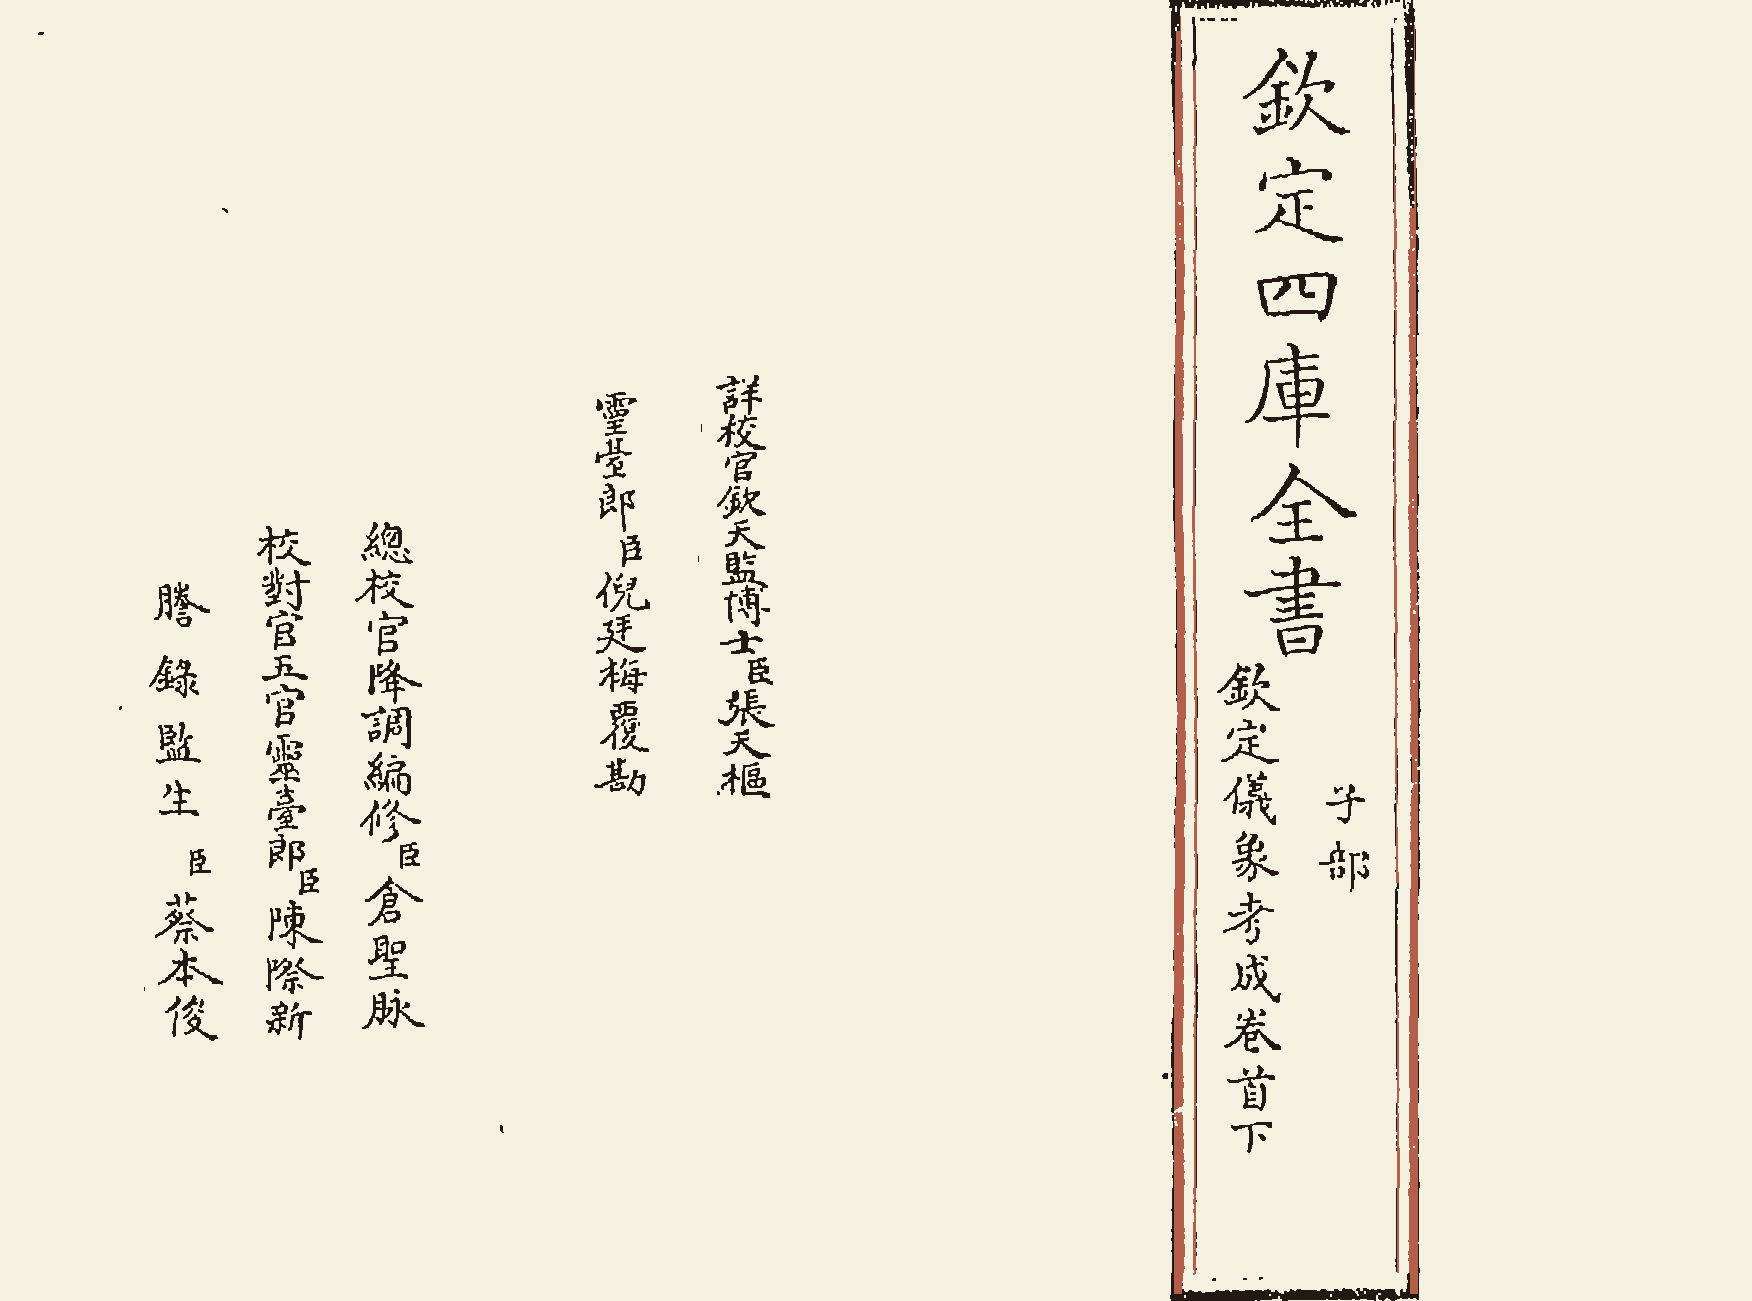
\includegraphics[width=\paperwidth,height=\paperheight,keepaspectratio]{img/0232.png}\clearpage
\begin{正文}
% ---- 册793 葉233 ----
\SetPageNumber{1}
欽定四庫全書\换行
欽定儀象考成卷首下\换行
御製璣衡撫辰儀説卷下\换行
　　用法\换行
　　算法\换行
\char"200B\relax\换行
\char"200B\relax\换行
\char"200B\relax\换行
\char"200B\relax\换行
\char"200B\relax\换行
\char"200B\relax\换行
\char"200B\relax\换行
\char"200B\relax\换行
\char"200B\relax\换行
\char"200B\relax\换行
\char"200B\relax
\par
% ---- 册793 葉236 ----
御製璣衡撫辰儀説卷下之一\换行
　用法\换行
　　測太陽時刻\换行
　　測日出入時刻及晝夜永短\换行
　　測太陽赤道緯度\换行
　　測午正太陽髙弧\换行
　　測太陽赤道經度\换行
　　測月星赤道經緯度\换行
　　測恒星求時刻\换行
　　測月五星求時刻\换行
　　測月星當中及偏度\换行
　　測月星出入地平時刻\换行
　　測南北真線\换行
　　測北極髙度\换行
　　測黄赤距度\换行
　　測黄白距度
\par
% ---- 册793 葉237 ----
　　測太陽時刻\换行
法以四遊圏東西推轉窺衡南北低昂令太陽從衡孔\换行
透光圓正或用薫黒玻璃置於下端衡孔視上端圓孔\换行
十字線正當太陽中心則窺衡與太陽參直乃視四遊\换行
圏下周指時度表臨於天常赤道之某時刻分即太陽\换行
時刻也若二分前後日影為赤道所礙則用窺衡上面\换行
立表測之\双列{\右小列{常時不為赤道所}\左小列{礙亦用此表為便}}若午正及卯酉前後日影\换行
為子午圏及龍柱所礙則用窺衡上面平行立表測之\换行
以四遊窺衡對凖太陽令上端表圓孔十字線影從下\换行
端表圓孔正中透出上端表直線影從下端表直縫正\换行
中透出\双列{\右小列{測時刻止用經度可止取直線影}\左小列{若測緯度則必取圓孔十字線影}}視指時度表\换行
所指即得太陽時刻若指時度表為子午圏所礙則易\换行
用借弧指時度表次用平行立表測定日影視借弧指\换行
時度表所指時刻加一小時即得太陽時刻盖借弧之\换行
長當遊旋赤道之十五度當天常赤道之一小時又借\换行
表在四遊圏之西所指時刻在本時前故加一小時即
\par
% ---- 册793 葉240 ----
為本時刻分也\换行
　　測日出入時刻及晝夜永短\换行
法於太陽出入地平時按前法測得太陽出入時刻乃\换行
計距午正前後若干刻分倍之即得晝刻計距子正前\换行
後若干刻分倍之即得夜刻\换行
　　測太陽赤道緯度\换行
法如前測凖太陽視窺衡下端指緯度表所指四遊圏\换行
右面距赤道度分即得太陽赤道緯度表指赤道北太\换行
陽緯度為在赤道南表指赤道南太陽緯度為在赤道\换行
北盖窺管以圓心為樞上端所窺在赤道北下端所指\换行
必在赤道南上端所窺在赤道南下端所指必在赤道\换行
北也\换行
　　測午正太陽髙弧\换行
法於午正時測得太陽赤道緯度在赤道北與赤道髙\换行
五十度五分相加在赤道南與赤道髙五十度五分相\换行
減即午正太陽髙弧也
\par
% ---- 册793 葉241 ----
　　測太陽赤道經度\换行
法用恒星作距測之取所知近午正前後一恒星\双列{\右小列{午正}\左小列{前後}}\换行
\双列{\右小列{取其𫎇氣少}\左小列{易得確凖也}}以其赤道經度之對衝用綰經度表於遊\换行
旋赤道綰定四遊圏\双列{\右小列{凡以儀器測星其上當星處為星}\左小列{之正位其下當人目處則星之對}}\换行
\双列{\右小列{冲故以星經度之對冲於}\左小列{遊旋赤道綰定四遊圏}}又任設一時用綰時度表於\换行
其時刻之對衝綰定天常赤道\双列{\右小列{天常環面乃日影所照}\左小列{之時其對冲則太陽所}}\换行
\双列{\右小列{臨之正位故於設時之對冲綰之如設丑正初}\左小列{刻則綰於未正初刻即太陽臨於丑正之位也}}乃将四\换行
逰圏帶定遊旋赤道用窺衡測凖距星隨之左旋𠉀至\换行
所設時刻\双列{\右小列{或鐘表或漏}\左小列{壺須得確凖}}視綰時度表對於遊旋赤道之\换行
某宫度分即太陽赤道經度也\双列{\右小列{環面時刻之對冲即太}\左小列{陽所臨之正位故其所}}\换行
\双列{\右小列{對遊旋赤道之宫}\左小列{度即太陽經度}}\换行
又法先以恒星作距測金星次以金星作距測太陽如\换行
金星晨見則於太陽未出之前取在金星西之一恒星\换行
作距以其赤道經度用平行線測經度表於遊旋赤道\换行
安定\双列{\右小列{三測皆係經度若距星之經度用對冲則測得之}\左小列{經度又須加減半周故距星不用對冲所測亦即}}\换行
\双列{\右小列{得本}\左小列{度也}}令一人用此平行線表窺定距星隨之左旋一人
\par
% ---- 册793 葉244 ----
用四遊窺衡測金星兩人同時測定乃視四遊圏指時\换行
度表所指遊旋赤道之宫度分即金星赤道經度次以\换行
金星赤道經度用平行線測經度表於遊旋赤道安定\换行
令一人窺定金星隨之左旋一人於太陽始出時用四\换行
遊窺衡測太陽乃視四遊圏指時度表所指遊旋赤道\换行
之宫度分即得太陽赤道經度若金星夕見則於太陽\换行
将入時任於某宫初度安定平行線測經度表令一人\换行
窺定金星又令一人用四遊窺衡測太陽視太陽距金\换行
星若干度記定俟太陽既入後取金星東之一恒星作\换行
距按前法測得金星赤道經度内減太陽距金星之度\换行
\双列{\右小列{星在東日}\左小列{在西故減}}即得太陽赤道經度也\双列{\右小列{太陽光大惟月及金}\左小列{星可以兩見然月有}}\换行
\双列{\右小列{視差不如用}\左小列{金星為凖也}}\换行
　　測月星赤道經緯度\换行
法於昏後曉前任設一時以本日太陽赤道經度與次\换行
日太陽赤道經度比例得本時太陽赤道經度\双列{\右小列{七政時}\左小列{憲書所}}\换行
\双列{\右小列{列乃子正之度子正後七政皆有行分故以本日子正}\左小列{之度分與次日子正之度分相減餘為一日十二時所}}
\par
% ---- 册793 葉245 ----
\双列{\右小列{行之分與設時距子正之時分為比例得設時距子}\左小列{正之行分加於本日子正之度分得本時之度分}}用\换行
綰時度表於遊旋赤道綰定又以所設時刻之對冲於\换行
天常赤道綰定𠉀至所設時刻用四遊窺衡測月星乃\换行
視指時度表所指遊旋赤道宫度加半周\双列{\右小列{環面時刻之}\左小列{對冲即為太}}\换行
\双列{\右小列{陽之正位環面之宮度却}\左小列{為月星之對冲故加半周}}即得所測月星赤道經度隨\换行
察指緯度表所指四遊圏距赤道南北度分即得所測\换行
月星赤道緯度也\双列{\右小列{緯之南北與前測}\左小列{太陽緯度法同}}\换行
又法用恒星作距測之以距星之赤道經度用平行線\换行
測經度表於遊旋赤道安定令一人用此平行線表窺\换行
定距星隨之左旋一人用四遊窺衡測月星兩人同時\换行
測定乃視指時度表所指遊旋赤道之度分即所測月\换行
星之赤道經度隨察指緯度表所指四遊圏之度分即\换行
得所測月星之赤道緯度也\换行
　　測恒星求時刻\换行
法先以恒星赤道經度用綰經度表於遊旋赤道綰定\换行
四遊圏次約計測時為某時依前法比例得本時太陽
\par
% ---- 册793 葉248 ----
赤道經度\双列{\右小列{太陽每日行一度於時為四分每一時行五}\左小列{分於時為二十秒故約計測量之時比例得}}\换行
\双列{\右小列{其時赤道經度即}\左小列{可用以測時刻也}}用綰時度表綰定遊旋赤道将四遊\换行
圏帶遊旋赤道推轉用窺衡測定恒星乃視綰時度表\换行
對於天常赤道之某時刻分加六時即太陽時刻也\双列{\右小列{天}\左小列{常}}\换行
\双列{\右小列{赤道之時刻乃日影對照之時故}\左小列{加六時始為太陽所臨之時刻也}}\换行
　　測月五星求時刻\换行
法以本時太陽赤道經度用綰時度表綰定遊旋赤道\换行
以月五星本時赤道經度之對冲用綰經度表於遊旋\换行
赤道綰定四遊圏将四遊圏帶遊旋赤道推轉用窺衡\换行
測定月星乃視綰時度表對於天常赤道之某時刻分\换行
加六時即得太陽時刻若太陽近子正前後綰時度表\换行
為子午圏所礙則向東或西借三十度綰定測之視所\换行
對時刻加減一時\双列{\右小列{向東借則加}\左小列{向西借則減}}即得太陽時刻若月五\换行
星近赤道或近午正前後為諸圏所礙則用窺管上面\换行
立表及平行立表測之與前測太陽時刻法同\换行
　　測月星當中及偏度
\par
% ---- 册793 葉249 ----
法以四遊窺衡隨時測月或星視指時度表當天常赤\换行
道之某時刻分記之\双列{\右小列{近午正則易用借弧}\左小列{指時度表加一小時}}午正為當中\换行
無偏度午正前為偏東午正後為偏西乃以距午時分\换行
變赤道度每一時為三十度每一小時為十五度每一\换行
分為十五分每一秒為十五秒共之為所偏度凡推月\换行
星當中及偏度者用此法測之則離合可辨凡有求時\换行
刻者用此法測定則時刻可推也\换行
　　測月星出入地平時刻\换行
法以本日子正月五星赤道經度或恒星經度之對冲\换行
用綰經度表於遊旋赤道綰定四遊圏又以本日子正\换行
太陽經度用綰時度表綰定遊旋赤道爰以四遊窺衡\换行
於月星出入地平時測之視綰時度表當天常赤道之\换行
某時刻分加六時為本日月星出入時刻之通數復計\换行
測時距本日子正後若干時刻比例得太陽行分變時\换行
\双列{\右小列{每一度為四分每十五分}\左小列{為一分每十五秒為一秒}}為太陽時差比例得月五星\换行
行分變時為月五星時差\双列{\右小列{恒星則無行}\左小列{分亦無時差}}乃於前所測月
\par
% ---- 册793 葉252 ----
星出入時刻之通數減太陽時差加月五星時差即得\换行
月星出入地平時刻盖日與月星測時皆用子正經度\换行
而子正後太陽有右旋之行分則時刻必差而早月五\换行
星亦有右旋之行分則時刻必差而遲\双列{\右小列{時刻左旋七政}\左小列{皆右旋太陽有}}\换行
\双列{\右小列{右旋之行分則測時太陽之經度必在所測時刻之前}\左小列{故差而早月五星有右旋之行分則測時月星之方位}}\换行
\双列{\右小列{必在所測時刻}\左小列{之後故差而遲}}故減太陽時差加月五星時差\双列{\右小列{若五星}\左小列{逆行則}}\换行
\双列{\右小列{時差}\左小列{亦減}}方為月星出入地平真時此與前測月星求時刻\换行
法同理設時可以預知故先求本時經度而後測月星\换行
出入難以懸定故先測而後加減時差其理相通其用\换行
尤便也\换行
　　測南北真線\换行
法於太陽出地平時測其距午東赤道度又於太陽入\换行
地平時測其距午西赤道度\双列{\右小列{測得太陽出入地平距午}\左小列{正前後若干時分變赤道}}\换行
\双列{\右小列{度即得距午正}\左小列{東西赤道度}}兩距午度相等則子午圏之向即南北\换行
真線若日出距午東之度多日入距午西之度少則子\换行
午圏之午正偏西若日出距午東之度少日入距午西
\par
% ---- 册793 葉253 ----
之度多則子午圏之午正偏東\双列{\右小列{此言午正乃子}\左小列{午圏之正南}}以兩測\换行
之距午度相減折半即所偏之赤道經度\双列{\右小列{若求地平偏}\左小列{度則用三角}}\换行
\双列{\右小列{法推之見算}\左小列{法第八則}}依所偏之度作線即南北真線也\换行
又法於冬至後測織女第一星昏刻此星當酉正之位\换行
以四遊圏安於酉正測其去極度若干\双列{\右小列{九十度内減赤}\左小列{道緯度餘即去}}\换行
\双列{\右小列{極}\左小列{度}}旦刻此星當卯正之位以四遊圏安於卯正測其去\换行
極度若干\双列{\右小列{織女星在赤道丑宫七度赤道北三十八度}\左小列{半冬至後半月内昏旦可以兩見故専取此}}\换行
\双列{\右小列{星測}\左小列{之}}兩去極度相等則子午圏之向即南北真線若卯\换行
正位測得去極度多酉正位測得去極度少則東逺西\换行
近即子午圈之北極偏西若卯正位測得去極度少酉\换行
正位測得去極度多則東近西逺即子午圈之北極偏\换行
東以兩測之去極度相減折半即所偏之赤道緯度\双列{\右小列{若}\左小列{求}}\换行
\双列{\右小列{地平偏度則用三角法}\左小列{推之見算法第十五則}}依所偏之度作線即南北真線\换行
也盖南北真線自北極過天頂平分赤道之地平上半\换行
周是為午正故向南測者以午正為凖向北測者以北\换行
極為凖太陽隨天左旋其出地入地距午必相等若其
\par
% ---- 册793 葉256 ----
不等必儀之午正偏也恒星繞地左旋其在東在西去\换行
極必相等若其不等必儀之北極偏也依其偏度正之\换行
則南北真線得矣又按渾儀經緯與天同象測太陽亦\换行
可用緯度測恒星亦可用經度然不及右二法之簡明\换行
推測精熟法理自見今不具悉也\换行
　　測北極髙度\换行
法於冬至前後以四遊圏安於正北測天權星\双列{\右小列{即北斗}\左小列{第四星}}\换行
昏刻此星在北極之下測其去極度若干旦刻此星在\换行
北極之上測其去極度若干\双列{\右小列{天權星今在赤道辰宫初}\左小列{度赤道北五十八度冬至}}\换行
\双列{\右小列{前後半月内昏旦可以}\左小列{兩見故専取此星測之}}兩去極度相等則儀之北極髙\换行
度與天合若在上之去極度少在下之去極度多則儀\换行
之北極差髙若在上之去極度多在下之去極度少則\换行
儀之北極差下以兩測之去極度相減折半即所差之\换行
地平緯度於儀之北極髙度加減之\双列{\右小列{差髙則減}\左小列{差下則加}}即天之\换行
北極髙度也盖天之北極無星故取大星之環繞北極\换行
上下者測之星之去極有定度則上下兩測之去極必
\par
% ---- 册793 葉257 ----
等若其不等則儀之髙下差也依其差度加減之則在\换行
天之北極髙度得矣又按舊法用地平緯儀測鉤陳大\换行
星以其在北極上下兩髙度相加折半得北極髙度取\换行
其距地髙無𫎇氣也今用渾儀測之則鉤陳大星為儀\换行
樞所礙須用借弧故取用天權星測其去極之較以備\换行
一例若以所測在北極上之去極度與所設北極髙度\换行
相加以所測在北極下之去極度與所設北極髙度相\换行
減得兩地平髙度相加折半得北極髙度與用鉤陳大\换行
星之理同\换行
　　測黄赤大距\换行
法於冬至日午正初刻測太陽在赤道南若干度分夏\换行
至日午正初刻測太陽在赤道北若干度分若冬至夏\换行
至皆在午正初刻則所測日距赤道南北之緯度即黄\换行
赤大距度若冬至夏至不正當午正則又用前測太陽\换行
赤道經度法測得太陽距冬夏至前後若干度分用有\换行
太陽赤道經緯度求黄赤交角之法\双列{\右小列{見算法}\左小列{第四則}}求得黄赤
\par
% ---- 册793 葉260 ----
交角即黄赤大距度也盖黄道與赤道斜交春秋分時\换行
太陽正當赤道春分後秋分前太陽在赤道北夏至而\换行
極北秋分後春分前太陽在赤道南冬至而極南故致\换行
日者必於冬夏二至今用弧線三角形法測得逐日之\换行
距緯皆可以推大距然春秋分前後黄道斜而緯差大\换行
以推大距其理𨼆而難知冬夏至前後黄道横而緯差\换行
微以推大距其象顯而易見故冬夏致日古今之通義\换行
也\换行
　　測黄白距限\双列{\右小列{距限即大距因大距又有大小故}\左小列{名距限以别之見數象考成後編}}\换行
法於春分日上弦秋分日下弦月距交九十度時測得\换行
月距赤道北若干度分春分日下弦秋分日上弦月距\换行
交九十度時測得月距赤道南若干度分與黄赤大距\换行
相減餘為黄白二道最大之距限又於冬至日望月距\换行
交九十度時測得月距赤道北若干度分夏至日望月\换行
距交九十度時測得月距赤道南若干度分與黄赤大\换行
距相減餘為黄白二道最小之距限盖白道與黄道斜
\par
% ---- 册793 葉261 ----
交月距交九十度則距黄道最逺故測黄白大距必於\换行
月距交九十度時然黄白大距與黄道成直角黄赤大\换行
距與赤道成直角惟冬夏二至黄道經圈與赤道經圈\换行
合為一線故測黄白大距又必於月當冬夏二至時\双列{\右小列{上}\左小列{編}}\换行
\双列{\右小列{専取月當夏至為其距地髙也}\左小列{若以對待而言則兼用冬夏至}}夫月距交九十度而又\换行
當冬夏二至則兩交必在春秋二分當是時而值兩弦\换行
則日必在春秋分而適當兩交值朔望則日必在冬夏\换行
至而距交九十度上編之法謂兩弦時交角大\双列{\右小列{交角之}\左小列{度即大}}\换行
\双列{\右小列{距}\左小列{度}}朔望時交角小後編之法謂日在兩交時交角大日\换行
距交九十度時交角小極二説之異致至此而得其合\换行
故測黄白大距必於春秋分兩弦冬夏至望日\双列{\右小列{朔日不}\左小列{見月故}}\换行
\双列{\右小列{惟用}\左小列{望日}}月距交九十度時測之春分之日上弦秋分之日\换行
下弦而月距交九十度是月當夏至而日在兩交也春\换行
分之日下弦秋分之日上弦而月距交九十度是月當\换行
冬至而日在兩交也以兩弦與日在兩交而論皆交角\换行
大冬至之日望而月距交九十度是月當夏至而日距
\par
% ---- 册793 葉264 ----
交九十度也夏至之日望而月距交九十度是月當冬\换行
至而日距交九十度也以朔望與日距交九十度而論\换行
皆交角小各測其距赤道度與黄赤大距相減則最大\换行
最小之黄白距限皆得矣按月行出黄道南為陽厯為\换行
正交\双列{\右小列{今為}\左小列{中交}}入黄道北為陰厯為中交\双列{\右小列{今為}\左小列{正交}}夏至在陰厯\换行
冬至在陽厯則月距赤道校黄道為逺故於所測距赤\换行
道度内減黄赤大距餘為黄白大距夏至在陽厯冬至\换行
在陰厯則月距赤道校黄道為近故於黄赤大距内減\换行
所測距赤道度餘為黄白大距又按古法黄白大距不\换行
逾六度弦望無殊故曰春秋致月今法交角有大小故\换行
又必兼於冬夏至測之也\换行
又法推得月離黄道冬夏至時預於前數刻或以太陽\换行
作距用綰時度表綰定時刻或以恒星作距用平行線\换行
測經度表對定距星皆以四遊圏指時度表對冬夏至\换行
宫度安定候月行至二至線上乃以窺衡測月距赤道\换行
南北緯度若干與黄赤大距相減餘為月距黄道南北
\par
% ---- 册793 葉265 ----
緯度以正交宫度與冬夏至宫度相減餘為月距正交\换行
黄道經度用有太陽赤道經緯度求黄赤交角之法\双列{\右小列{見}\左小列{算}}\换行
\双列{\右小列{法第}\左小列{四則}}求得交角度分即黄白距限盖月之緯度與黄道\换行
成直角其三角形之比例則黄道如赤道白道如黄道\换行
黄緯如赤緯黄白交角即如黄赤交角黄白大距即如\换行
黄赤大距也前法於分至弦望測月緯度乃測黄白大\换行
距正法然其時不易得此法於月離冬夏至時凡見月\换行
即可測叅之弦望與日距交之逺近則交角有大小之\换行
故亦可得而稽矣\换行
\char"200B\relax\换行
\char"200B\relax\换行
\char"200B\relax\换行
\char"200B\relax\换行
\char"200B\relax\换行
\char"200B\relax\换行
\char"200B\relax
\par
% ---- 册793 葉268 ----
御製璣衡撫辰儀説下之二\换行
　算法\换行
　　有太陽赤道緯度求午正髙弧\换行
　　有太陽視髙弧求午正晷影\换行
　　有太陽赤道緯度求赤道經度\换行
　　有太陽赤道經緯度求黄赤大距\换行
　　有太陽赤道緯度求黄道經度\换行
　　有太陽赤道緯度求出入地平及晝夜時刻\换行
　　有太陽赤道緯度求昏旦時刻\换行
　　有太陽赤道緯度求太陽出入地平偏度\双列{\右小列{二題}\左小列{}}\换行
　　有時刻有太陽赤道緯度求地平經緯度\换行
　　有節氣有太陽午正髙弧求交節氣時刻\换行
　　有日月星赤道經度求月星當中時刻\换行
　　有日月星赤道經度有時刻求月星當中及偏度\换行
　　有日月星赤道經緯度求月星出入地平時刻\换行
　　有月星赤道經緯度求黄道經緯度
\par
% ---- 册793 葉269 ----
　　有月星距午赤道度有赤道緯度求地平經緯度\换行
　　有二星赤道經緯度求二星斜距度\换行
　　有日月五星視髙度求實髙度\换行
\char"200B\relax\换行
\char"200B\relax\换行
\char"200B\relax\换行
\char"200B\relax\换行
\char"200B\relax\换行
\char"200B\relax\换行
\char"200B\relax\换行
\char"200B\relax\换行
\char"200B\relax\换行
\char"200B\relax\换行
\char"200B\relax\换行
\char"200B\relax\换行
\char"200B\relax
\par
\end{正文}\clearpage
\contentSetup{n-char-per-col = 20, n-column = 9}
\begin{正文}
\end{正文}
\嵌图{259.22pt}{211.13pt}{687.10pt}{283.77pt}{img/0272.png}
\begin{正文}
% ---- 册793 葉272 ----
\SetPageNumber{20}
設如北極出地三十九度五十五分午正初刻測得\换行
　太陽距赤道北十五度求髙弧幾何\换行
　　　　　　　　　　如圖甲為天頂甲乙丙丁\换行
　　　　　　　　　　為子午圏乙丙為地平丁\换行
　　　　　　　　　　為北極戊己為赤道丁丙\换行
　　　　　　　　　　為北極出地三十九度五\换行
　　　　　　　　　　十五分戊乙為赤道髙五\换行
　　　　　　　　　　十度五分庚為太陽庚戊\换行
　　　　　　　　　　為太陽距赤道北十五度\换行
　　　　　　　　　　庚乙為太陽髙弧太陽正\换行
　　　　　　　　　　當午正赤經與髙弧合則\换行
　　　　　　　　　　以庚戊距緯與戊乙赤道\换行
　　　　　　　　　　髙度相加得庚乙六十五\换行
　　　　　　　　　　度五分為午正太陽髙度\换行
　　　　　　　　　　若太陽距赤道南則以距\换行
　　　　　　　　　　緯與赤道髙度相減即午\换行
　　　　　　　　　　正太陽髙度也\换行
設如測得午正太陽髙弧四十度中表髙八尺求影
\par
\end{正文}\clearpage
\嵌图{211.28pt}{218.24pt}{643.91pt}{276.65pt}{img/0273.png}
\begin{正文}
% ---- 册793 葉273 ----
\SetPageNumber{21}
　長幾何\换行
　　　　　　　　　　法以半徑一千萬為一率\换行
　　　　　　　　　　午正太陽髙弧四十度之\换行
　　　　　　　　　　餘切一千一百九十一萬\换行
　　　　　　　　　　七千五百三十六為二率\换行
　　　　　　　　　　表髙八尺為三率求得四\换行
　　　　　　　　　　率九尺五寸三分四釐零\换行
　　　　　　　　　　二絲八忽八微為所求之\换行
　　　　　　　　　　影長也如圖甲乙為中表\换行
　　　　　　　　　　之髙丙為太陽丁為中影\换行
　　　　　　　　　　心甲丁乙角為午正太陽\换行
　　　　　　　　　　髙度乙丁為影長則以丁\换行
　　　　　　　　　　戊半徑與太陽髙弧餘切\换行
　　　　　　　　　　戊已之比同於甲乙表髙\换行
　　　　　　　　　　與乙丁影長之比也\换行
設如春分後測得太陽距赤道北十五度黄赤交角\换行
　二十三度二十九分求赤道經度幾何\换行
　　　　　　　　　　如圖甲乙丙丁為赤道甲
\par
\end{正文}\clearpage
\嵌图{171.14pt}{215.35pt}{820.73pt}{279.54pt}{img/0276.png}
\begin{正文}
% ---- 册793 葉276 ----
\SetPageNumber{22}
\插图页
　　　　　　　　　　戊丙己為黄道相交於甲\换行
　　　　　　　　　　丙甲為春分丙為秋分戊\换行
　　　　　　　　　　為夏至己為冬至庚為北\换行
　　　　　　　　　　極辛為南極庚戊乙辛己\换行
　　　　　　　　　　丁為過二極二至經圈乙\换行
　　　　　　　　　　至戊丁至己俱二十三度\换行
　　　　　　　　　　二十九分為黄赤大距即\换行
　　　　　　　　　　甲丙黄赤二道相交之角\换行
　　　　　　　　　　壬為太陽甲壬為太陽距\换行
\恢复丝栏
　　　　　　　　　　春分後黄道經度自庚辛\换行
　　　　　　　　　　南北二極過太陽壬作庚\换行
　　　　　　　　　　壬癸辛赤極經圏交赤道\换行
　　　　　　　　　　於癸癸點為太陽所當赤\换行
　　　　　　　　　　道宫度甲癸為太陽距春\换行
　　　　　　　　　　分後赤道經度壬癸為太\换行
　　　　　　　　　　陽距赤道北十五度法用\换行
　　　　　　　　　　甲壬癸正弧三角形有甲\换行
　　　　　　　　　　角黄赤交角有癸直角有
\par
\end{正文}\clearpage
\嵌图{176.39pt}{207.01pt}{769.93pt}{287.88pt}{img/0277.png}
\begin{正文}
% ---- 册793 葉277 ----
\SetPageNumber{23}
\插图页
　　　　　　　　　　壬癸距緯求甲癸赤道度\换行
　　　　　　　　　　以甲角二十三度二十九\换行
　　　　　　　　　　分之乙子正切四百三十\换行
　　　　　　　　　　四萬四千六百六十六為\换行
　　　　　　　　　　一率乙丑半徑一千萬為\换行
　　　　　　　　　　二率壬癸距緯十五度之\换行
　　　　　　　　　　癸寅正切二百六十七萬\换行
　　　　　　　　　　九千四百九十二為三率\换行
　　　　　　　　　　求得四率六百一十六萬\换行
\恢复丝栏
　　　　　　　　　　七千三百一十四為甲癸\换行
　　　　　　　　　　弧之正弦癸卯檢表得三\换行
　　　　　　　　　　十八度四分四十秒即甲\换行
　　　　　　　　　　癸太陽距春分後赤道經\换行
　　　　　　　　　　度與甲丁春分距冬至三\换行
　　　　　　　　　　宫相加得四宫八度四分\换行
　　　　　　　　　　四十秒即太陽赤道宫度\换行
　　　　　　　　　　也\换行
設如春分後測得太陽距赤道北十五度距春分後
\par
\end{正文}\clearpage
\嵌图{268.26pt}{209.25pt}{723.62pt}{285.65pt}{img/0280.png}
\begin{正文}
% ---- 册793 葉280 ----
\SetPageNumber{24}
　赤道經度三十八度四分四十秒求黄赤大距度\换行
　幾何\换行
　　　　　　　　　　如圖甲為春分甲角為黄\换行
　　　　　　　　　　赤交角當戊乙黄赤大距\换行
　　　　　　　　　　壬為太陽壬癸為太陽距\换行
　　　　　　　　　　赤道北十五度甲癸為太\换行
　　　　　　　　　　陽距春分後赤道經度三\换行
　　　　　　　　　　十八度四分四十秒用甲\换行
　　　　　　　　　　壬癸正弧三角形以甲癸\换行
　　　　　　　　　　赤道三十八度四分四十\换行
　　　　　　　　　　秒之癸卯正弦六百一十\换行
　　　　　　　　　　六萬七千三百一十四為\换行
　　　　　　　　　　一率壬癸距緯十五度之\换行
　　　　　　　　　　寅癸正切二百六十七萬\换行
　　　　　　　　　　九千四百九十二為二率\换行
　　　　　　　　　　乙丑半徑一千萬為三率\换行
　　　　　　　　　　求得四率四百三十四萬\换行
　　　　　　　　　　六千六百六十六為甲角
\par
\end{正文}\clearpage
\嵌图{598.94pt}{210.20pt}{392.93pt}{284.70pt}{img/0281.png}
\嵌图{144.29pt}{217.63pt}{132.27pt}{277.27pt}{img/0281_1.png}
\begin{正文}
% ---- 册793 葉281 ----
\SetPageNumber{25}
　　　　　　　　　　之正切乙子檢表得二十\换行
　　　　　　　　　　三度二十九分即甲角黄\换行
　　　　　　　　　　赤大距度也\换行
設如春分後測得太陽距赤道北十五度黄赤交角\换行
　二十三度二十九分求黄道經度幾何\换行
　　　　　　　　　　如圖甲為春分甲角為黄\换行
　　　　　　　　　　赤交角二十三度二十九\换行
　　　　　　　　　　分壬為太陽甲壬為太陽\换行
　　　　　　　　　　距春分後黄道經度壬癸\换行
　　　　　　　　　　為距赤道北十五度用甲\换行
　　　　　　　　　　壬癸正弧三角形有甲角\换行
　　　　　　　　　　黄赤交角有癸直角有壬\换行
　　　　　　　　　　癸距緯求甲壬黄道度以\换行
　　　　　　　　　　甲角二十三度二十九分\换行
　　　　　　　　　　之戊辰正弦三百九十八\换行
　　　　　　　　　　萬四千八百二十三為一\换行
　　　　　　　　　　率戊丑半徑一千萬為二\换行
　　　　　　　　　　率壬癸距緯十五度之壬
\par
\end{正文}\clearpage
\嵌图{723.65pt}{204.84pt}{268.22pt}{290.06pt}{img/0284.png}
\嵌图{167.32pt}{219.20pt}{382.61pt}{275.69pt}{img/0284_1.png}
\begin{正文}
% ---- 册793 葉284 ----
\SetPageNumber{26}
　　　　　　　　　　巳正弦二百五十八萬八\换行
　　　　　　　　　　千一百九十為三率求得\换行
　　　　　　　　　　四率六百四十九萬五千\换行
　　　　　　　　　　一百一十九為甲壬弧之\换行
　　　　　　　　　　正弦壬午檢表得四十度\换行
　　　　　　　　　　三十分十七秒即甲壬太\换行
　　　　　　　　　　陽距春分後黄道經度與\换行
　　　　　　　　　　甲已春分距冬至三宫相\换行
　　　　　　　　　　加得四宫十度三十分十\换行
　　　　　　　　　　七秒即太陽黄道宫度也\换行
設如北極出地三十九度五十五分測得太陽距赤\换行
　道北十五度求出入地平及晝夜時刻\换行
　　　　　　　　　　如圖甲為天頂甲乙丙丁\换行
　　　　　　　　　　為子午圏乙丙為地平丁\换行
　　　　　　　　　　為北極丁丙為北極出地\换行
　　　　　　　　　　三十九度五十五分戊己\换行
　　　　　　　　　　為赤道戊乙為赤道髙五\换行
　　　　　　　　　　十度零五分庚為太陽庚
\par
\end{正文}\clearpage
\嵌图{163.37pt}{218.18pt}{386.56pt}{276.72pt}{img/0285.png}
\begin{正文}
% ---- 册793 葉285 ----
\SetPageNumber{27}
　　　　　　　　　　辛為太陽距赤道北十五\换行
　　　　　　　　　　度壬為卯正酉正之位辛\换行
　　　　　　　　　　壬為日出入在卯前酉後\换行
　　　　　　　　　　赤道度用庚辛壬正弧三\换行
　　　　　　　　　　角形有辛直角有壬角赤\换行
　　　　　　　　　　道髙度有庚辛邊求辛壬\换行
　　　　　　　　　　邊以壬角五十度五分之\换行
　　　　　　　　　　正切一千一百九十五萬\换行
　　　　　　　　　　二千七百九十九為一率\换行
　　　　　　　　　　半徑一千萬為二率庚辛\换行
　　　　　　　　　　十五度之正切二百六十\换行
　　　　　　　　　　七萬九千四百九十二為\换行
　　　　　　　　　　三率求得四率二百二十\换行
　　　　　　　　　　四萬一千七百二十八為\换行
　　　　　　　　　　辛壬弧之正弦檢表得十\换行
　　　　　　　　　　二度五十七分十五秒即\换行
　　　　　　　　　　辛壬弧為日出入在卯前\换行
　　　　　　　　　　酉後赤道度變時得三刻
\par
\end{正文}\clearpage
\嵌图{171.14pt}{215.05pt}{820.73pt}{279.84pt}{img/0288.png}
\begin{正文}
% ---- 册793 葉288 ----
\SetPageNumber{28}
\插图页
　　　　　　　　　　六分四十九秒為卯前酉\换行
　　　　　　　　　　後分以減卯正得日出卯\换行
　　　　　　　　　　初初刻八分十一秒以加\换行
　　　　　　　　　　酉正得日入酉正三刻六\换行
　　　　　　　　　　分四十九秒復倍卯前酉\换行
　　　　　　　　　　後分得六刻十三分三十\换行
　　　　　　　　　　八秒與四十八刻相加得\换行
　　　　　　　　　　五十四刻十三分三十八\换行
　　　　　　　　　　秒為晝刻與四十八刻相\换行
\恢复丝栏
　　　　　　　　　　減得四十一刻一分二十\换行
　　　　　　　　　　二秒為夜刻也又法求己\换行
　　　　　　　　　　辛日出入距子正前後赤\换行
　　　　　　　　　　道度用丁丙庚正弧三角\换行
　　　　　　　　　　形有丙直角有丁丙北極\换行
　　　　　　　　　　出地度有丁庚日距北極\换行
　　　　　　　　　　度求丁角以丁庚七十五\换行
　　　　　　　　　　度之正切三千七百三十\换行
　　　　　　　　　　二萬零五百零八為一率
\par
\end{正文}\clearpage
\嵌图{612.78pt}{223.00pt}{379.10pt}{271.90pt}{img/0289.png}
\嵌图{163.01pt}{219.31pt}{386.92pt}{275.58pt}{img/0289_1.png}
\begin{正文}
% ---- 册793 葉289 ----
\SetPageNumber{29}
　　　　　　　　　　丁丙三十九度五十五分\换行
　　　　　　　　　　之正切八百三十六萬六\换行
　　　　　　　　　　千二百四十二為二率半\换行
　　　　　　　　　　徑一千萬為三率求得四\换行
　　　　　　　　　　率二百二十四萬一千七\换行
　　　　　　　　　　百二十八為丁角之餘弦\换行
　　　　　　　　　　檢表得七十七度二分四\换行
　　　　　　　　　　十五秒即辛已弧為日出\换行
　　　　　　　　　　入距子正前後赤道度變\换行
　　　　　　　　　　時得五小時零八分十一\换行
　　　　　　　　　　秒為日出入距子正前後\换行
　　　　　　　　　　分自子正起算為卯初初\换行
　　　　　　　　　　刻八分十一秒即日出時\换行
　　　　　　　　　　刻與二十四小時相減得\换行
　　　　　　　　　　酉正三刻六分四十九秒\换行
　　　　　　　　　　為日入時刻復倍日出入\换行
　　　　　　　　　　距子正前後分得四十一\换行
　　　　　　　　　　刻一分二十二秒為夜刻
\par
\end{正文}\clearpage
\嵌图{605.32pt}{212.83pt}{386.56pt}{282.06pt}{img/0292.png}
\begin{正文}
% ---- 册793 葉292 ----
\SetPageNumber{30}
　　　　　　　　　　與九十六刻相減餘五十\换行
　　　　　　　　　　四刻十三分三十八秒為\换行
　　　　　　　　　　晝刻也\换行
設如北極出地三十九度五十五分測得太陽距赤\换行
　道北十五度求昏旦時刻\换行
　　　　　　　　　　如圖甲為天頂甲乙丙丁\换行
　　　　　　　　　　為子午圈乙丙為地平丁\换行
　　　　　　　　　　為北極丁丙為北極出地\换行
　　　　　　　　　　三十九度五十五分甲丁\换行
\插图页
　　　　　　　　　　為北極距天頂五十度五\换行
　　　　　　　　　　分戊己為赤道庚為太陽\换行
　　　　　　　　　　庚辛為太陽距赤道北十\换行
　　　　　　　　　　五度丁庚為太陽距北極\换行
　　　　　　　　　　七十五度壬癸為太陽隨\换行
　　　　　　　　　　天西轉之赤道距等圈庚\换行
　　　　　　　　　　子為昏旦曚影限十八度\换行
　　　　　　　　　　甲庚為太陽距天頂一百\换行
　　　　　　　　　　零八度丑寅為地平下曚
\恢复丝栏
\par
\end{正文}\clearpage
\嵌图{171.43pt}{217.40pt}{820.44pt}{277.49pt}{img/0293.png}
\begin{正文}
% ---- 册793 葉293 ----
\SetPageNumber{31}
\插图页
　　　　　　　　　　影距等圈辛點為太陽所\换行
　　　　　　　　　　當昏旦時刻戊辛為太陽\换行
　　　　　　　　　　距午正前後赤道度用甲\换行
　　　　　　　　　　庚丁斜弧三角形有甲丁\换行
　　　　　　　　　　邊北極距天頂有丁庚邊\换行
　　　　　　　　　　日距北極有甲庚邊日距\换行
　　　　　　　　　　天頂求丁角距午赤道度\换行
　　　　　　　　　　以夾丁角之丁庚邊七十\换行
　　　　　　　　　　五度與甲丁邊五十度五\换行
\恢复丝栏
　　　　　　　　　　分相加得一百二十五度\换行
　　　　　　　　　　五分為總弧其餘弦五百\换行
　　　　　　　　　　七十四萬七千六百七十\换行
　　　　　　　　　　二又以甲丁丁庚二邊相\换行
　　　　　　　　　　減餘二十四度五十五分\换行
　　　　　　　　　　為較弧其餘弦九百零六\换行
　　　　　　　　　　萬九千二百一十五兩餘\换行
　　　　　　　　　　弦相加\双列{\右小列{總弧較弧一過象}\左小列{限一不過象限則}}\换行
　　　　　　　　　　\双列{\右小列{兩餘弦相加若兩弧俱不}\左小列{過象限或俱過象限則兩}}
\par
\end{正文}\clearpage
\嵌图{192.65pt}{215.83pt}{799.22pt}{279.06pt}{img/0296.png}
\begin{正文}
% ---- 册793 葉296 ----
\SetPageNumber{32}
\插图页
　　　　　　　　　　\双列{\右小列{餘弦}\左小列{相減}}得一千四百八十一\换行
　　　　　　　　　　萬六千八百八十七折半\换行
　　　　　　　　　　得七百四十萬零八千四\换行
　　　　　　　　　　百四十四為中數為一率\换行
　　　　　　　　　　以對丁角之甲庚邊一百\换行
　　　　　　　　　　零八度之大矢一千三百\换行
　　　　　　　　　　零九萬零一百七十\双列{\右小列{餘弦}\左小列{與半}}\换行
　　　　　　　　　　\双列{\右小列{徑相加}\左小列{得大矢}}與較弧二十四度\换行
　　　　　　　　　　五十五分之正矢\双列{\右小列{餘弦與}\左小列{半徑相}}\换行
\恢复丝栏
　　　　　　　　　　\双列{\右小列{減得}\左小列{正矢}}九百三十萬零七百\换行
　　　　　　　　　　八十五相減餘一千二百\换行
　　　　　　　　　　一十五萬九千三百八十\换行
　　　　　　　　　　五為矢較為二率半徑一\换行
　　　　　　　　　　千萬為三率求得四率一\换行
　　　　　　　　　　千六百四十一萬二千八\换行
　　　　　　　　　　百七十三為丁角之大矢\换行
　　　　　　　　　　\双列{\右小列{凡矢過於半徑者為}\左小列{大矢其角即為鈍角}}内減\换行
　　　　　　　　　　半徑一千萬餘六百四十
\par
\end{正文}\clearpage
\嵌图{182.48pt}{211.52pt}{809.40pt}{283.38pt}{img/0297.png}
\begin{正文}
% ---- 册793 葉297 ----
\SetPageNumber{33}
\插图页
　　　　　　　　　　一萬二千八百七十三為\换行
　　　　　　　　　　丁角之餘弦檢表得五十\换行
　　　　　　　　　　度六分四十四秒與半周\换行
　　　　　　　　　　相減餘一百二十九度五\换行
　　　　　　　　　　十三分十六秒為丁角度\换行
　　　　　　　　　　即旦刻太陽距午前昏刻\换行
　　　　　　　　　　太陽距午後赤道度變時\换行
　　　　　　　　　　得八小時二刻九分三十\换行
　　　　　　　　　　三秒與午正十二小時相\换行
\恢复丝栏
　　　　　　　　　　減得寅初一刻五分二十\换行
　　　　　　　　　　七秒即旦刻與午正十二\换行
　　　　　　　　　　小時相加得戌正二刻九\换行
　　　　　　　　　　分三十三秒即昏刻也如\换行
　　　　　　　　　　圖丁庚與丁甲相加得甲\换行
　　　　　　　　　　癸為總弧\双列{\右小列{丁庚丁癸丁壬}\左小列{三弧同為癸壬}}\换行
　　　　　　　　　　\双列{\右小列{距等圏所截}\左小列{故其度相等}}其正弦為癸\换行
　　　　　　　　　　卯餘弦為卯辰丁庚與丁\换行
　　　　　　　　　　甲相減餘甲壬為較弧其
\par
\end{正文}\clearpage
\嵌图{167.23pt}{203.63pt}{824.64pt}{291.26pt}{img/0300.png}
\begin{正文}
% ---- 册793 葉300 ----
\SetPageNumber{34}
\插图页
　　　　　　　　　　正弦為壬己餘弦為己辰\换行
　　　　　　　　　　以卯辰與己辰兩餘弦相\换行
　　　　　　　　　　加得巳卯折半得己午與\换行
　　　　　　　　　　未申等為中數又對丁角\换行
　　　　　　　　　　之甲庚邊與甲丑甲寅等\换行
　　　　　　　　　　其正弦為丑酉或寅酉餘\换行
　　　　　　　　　　弦為酉辰大矢為甲酉以\换行
　　　　　　　　　　甲酉與甲壬較弧之正矢\换行
　　　　　　　　　　甲已相減餘己酉與戌庚\换行
\恢复丝栏
　　　　　　　　　　等為矢較遂成壬庚戌與\换行
　　　　　　　　　　壬申未同式兩勾股形故\换行
　　　　　　　　　　未申與戌庚之比必同於\换行
　　　　　　　　　　壬申與壬庚之比也又戊\换行
　　　　　　　　　　辰為半徑壬申為距等圈\换行
　　　　　　　　　　之半徑壬庚與戊辛兩叚\换行
　　　　　　　　　　同為丁庚辛赤道經圏之\换行
　　　　　　　　　　所分則壬申與壬庚之比\换行
　　　　　　　　　　原同於戊辰與戊辛之比
\par
\end{正文}\clearpage
\嵌图{155.20pt}{208.44pt}{394.73pt}{286.46pt}{img/0301.png}
\begin{正文}
% ---- 册793 葉301 ----
\SetPageNumber{35}
\插图页
　　　　　　　　　　是以中數未申與矢較戌\换行
　　　　　　　　　　庚之比即同於半徑戊辰\换行
　　　　　　　　　　與丁角大矢戊辛之比也\换行
　　　　　　　　　　既得戊辛大矢内減戊辰\换行
　　　　　　　　　　半徑餘辛辰即丁外角餘\换行
　　　　　　　　　　弦檢表得丁外角所當辛\换行
　　　　　　　　　　巳弧之度復與半周相減\换行
　　　　　　　　　　即得丁角所當戊辛弧之\换行
　　　　　　　　　　度也\换行
\恢复丝栏
設如北極出地三十九度五十五分太陽出地平時\换行
　測得距赤道北十五度求地平偏度幾何\换行
　　　　　　　　　　如圖甲為天頂甲乙丙丁\换行
　　　　　　　　　　為子午圈乙丙為地平丁\换行
　　　　　　　　　　為北極丁丙為北極出地\换行
　　　　　　　　　　三十九度五十五分戊己\换行
　　　　　　　　　　為赤道庚為太陽庚辛為\换行
　　　　　　　　　　太陽距赤道北十五度壬\换行
　　　　　　　　　　為卯正庚壬為日出地平
\par
\end{正文}\clearpage
\嵌图{604.60pt}{218.75pt}{250.59pt}{276.15pt}{img/0304.png}
\嵌图{164.41pt}{215.08pt}{385.52pt}{279.82pt}{img/0304_1.png}
\begin{正文}
% ---- 册793 葉304 ----
\SetPageNumber{36}
　　　　　　　　　　偏度用庚辛壬正弧三角\换行
　　　　　　　　　　形有辛直角有壬角赤道\换行
　　　　　　　　　　髙度有庚辛邊求庚壬邊\换行
　　　　　　　　　　以壬角五十度五分之正\换行
　　　　　　　　　　弦七百六十六萬九千七\换行
　　　　　　　　　　百八十五為一率半徑一\换行
　　　　　　　　　　千萬為二率庚辛十五度\换行
　　　　　　　　　　之正弦二百五十八萬八\换行
　　　　　　　　　　千一百九十為三率求得\换行
　　　　　　　　　　四率三百三十七萬四千\换行
　　　　　　　　　　五百二十七為庚壬弧之\换行
　　　　　　　　　　正弦檢表得十九度四十\换行
　　　　　　　　　　三分十八秒為庚壬弧度\换行
　　　　　　　　　　即太陽出地平時正東偏\换行
　　　　　　　　　　北之度也\换行
設如北極出地三十九度五十五分太陽入地平時\换行
　測得距赤道南十五度求地平偏度㡬何\换行
　　　　　　　　　　如圖甲為天頂甲乙丙丁
\par
\end{正文}\clearpage
\嵌图{167.49pt}{205.29pt}{824.39pt}{289.61pt}{img/0305.png}
\begin{正文}
% ---- 册793 葉305 ----
\SetPageNumber{37}
\插图页
　　　　　　　　　　為子午圏乙丙為地平丁\换行
　　　　　　　　　　為北極丁丙為北極出地\换行
　　　　　　　　　　三十九度五十五分戊己\换行
　　　　　　　　　　為赤道庚為太陽庚辛為\换行
　　　　　　　　　　太陽距赤道南十五度壬\换行
　　　　　　　　　　為酉正庚壬為日入地平\换行
　　　　　　　　　　偏度用辛庚壬正弧三角\换行
　　　　　　　　　　形有辛直角有壬角赤道\换行
　　　　　　　　　　髙度有庚辛邊求庚壬邊\换行
\恢复丝栏
　　　　　　　　　　以壬角五十度五分之正\换行
　　　　　　　　　　弦七百六十六萬九千七\换行
　　　　　　　　　　百八十五為一率半徑一\换行
　　　　　　　　　　千萬為二率庚辛十五度\换行
　　　　　　　　　　之正弦二百五十八萬八\换行
　　　　　　　　　　千一百九十為三率求得\换行
　　　　　　　　　　四率三百三十七萬四千\换行
　　　　　　　　　　五百二十七為庚壬弧之\换行
　　　　　　　　　　正弦檢表得十九度四十
\par
\end{正文}\clearpage
\嵌图{597.14pt}{211.89pt}{394.73pt}{283.00pt}{img/0308.png}
\嵌图{147.59pt}{217.40pt}{128.97pt}{277.49pt}{img/0308_1.png}
\begin{正文}
% ---- 册793 葉308 ----
\SetPageNumber{38}
　　　　　　　　　　三分十八秒為庚壬弧度\换行
　　　　　　　　　　即太陽入地平時正西偏\换行
　　　　　　　　　　南之度也\换行
設如北極出地三十九度五十五分己正初刻測得\换行
　太陽距赤道北十五度求地平經緯度各㡬何\换行
　　　　　　　　　　如圖甲為天頂甲乙丙丁\换行
　　　　　　　　　　為子午圏乙丙為地平丁\换行
　　　　　　　　　　為北極戊己為赤道丁丙\换行
　　　　　　　　　　為北極出地三十九度五\换行
　　　　　　　　　　十五分甲丁為北極距天\换行
　　　　　　　　　　頂五十度五分庚為太陽\换行
　　　　　　　　　　庚辛為太陽距赤道北十\换行
　　　　　　　　　　五度丁庚為太陽距北極\换行
　　　　　　　　　　七十五度辛為己正初刻\换行
　　　　　　　　　　戊辛為太陽距午東赤道\换行
　　　　　　　　　　度三十度即丁角甲庚為\换行
　　　　　　　　　　太陽距天頂庚壬為太陽\换行
　　　　　　　　　　髙弧即地平緯度乙壬為
\par
\end{正文}\clearpage
\嵌图{171.14pt}{215.78pt}{820.73pt}{279.11pt}{img/0309.png}
\begin{正文}
% ---- 册793 葉309 ----
\SetPageNumber{39}
\插图页
　　　　　　　　　　太陽正南偏東地平經度\换行
　　　　　　　　　　即甲角之外角用甲丁庚\换行
　　　　　　　　　　斜弧三角形有丁角距午\换行
　　　　　　　　　　東赤道度有甲丁北極距\换行
　　　　　　　　　　天頂有丁庚太陽距北極\换行
　　　　　　　　　　求甲庚邊及甲角度乃自\换行
　　　　　　　　　　太陽庚點作庚癸垂弧於\换行
　　　　　　　　　　形外補成丁庚癸甲庚癸\换行
　　　　　　　　　　兩正弧三角形先用丁庚\换行
\恢复丝栏
　　　　　　　　　　癸形以半徑一千萬為一\换行
　　　　　　　　　　率丁角三十度之餘弦八\换行
　　　　　　　　　　百六十六萬零二百五十\换行
　　　　　　　　　　四為二率丁庚七十五度\换行
　　　　　　　　　　之正切三千七百三十二\换行
　　　　　　　　　　萬零五百零八為三率求\换行
　　　　　　　　　　得四率三千二百三十二\换行
　　　　　　　　　　萬零五百零八為丁癸弧\换行
　　　　　　　　　　之正切檢表得七十二度
\par
\end{正文}\clearpage
\嵌图{175.38pt}{210.18pt}{816.50pt}{284.72pt}{img/0312.png}
\begin{正文}
% ---- 册793 葉312 ----
\SetPageNumber{40}
\插图页
　　　　　　　　　　四十八分二十八秒即丁\换行
　　　　　　　　　　癸弧内減甲丁五十度五\换行
　　　　　　　　　　分餘二十二度四十三分\换行
　　　　　　　　　　二十八秒即甲癸弧又以\换行
　　　　　　　　　　半徑一千萬為一率丁角\换行
　　　　　　　　　　三十度之正切五百七十\换行
　　　　　　　　　　七萬三千五百零三為二\换行
　　　　　　　　　　率丁癸七十二度四十八\换行
　　　　　　　　　　分二十八秒之正弦九百\换行
\恢复丝栏
　　　　　　　　　　五十五萬三千一百八十\换行
　　　　　　　　　　四為三率求得四率五百\换行
　　　　　　　　　　五十一萬五千五百三十\换行
　　　　　　　　　　四為庚癸弧之正切次用\换行
　　　　　　　　　　甲庚癸形以甲癸二十二\换行
　　　　　　　　　　度四十三分二十八秒之\换行
　　　　　　　　　　正弦三百八十六萬二千\换行
　　　　　　　　　　九百九十六為一率前所\换行
　　　　　　　　　　得庚癸弧之正切五百五
\par
\end{正文}\clearpage
\嵌图{163.54pt}{209.93pt}{828.33pt}{284.96pt}{img/0313.png}
\begin{正文}
% ---- 册793 葉313 ----
\SetPageNumber{41}
\插图页
　　　　　　　　　　十一萬五千五百三十四\换行
　　　　　　　　　　為二率半徑一千萬為三\换行
　　　　　　　　　　率求得四率一千四百二\换行
　　　　　　　　　　十七萬七千八百六十六\换行
　　　　　　　　　　為甲角之正切檢表得五\换行
　　　　　　　　　　十四度五十九分三十五\换行
　　　　　　　　　　秒為甲角度即太陽正南\换行
　　　　　　　　　　偏東地平經度又以甲角\换行
　　　　　　　　　　五十四度五十九分三十\换行
\恢复丝栏
　　　　　　　　　　五秒之餘弦五百七十三\换行
　　　　　　　　　　萬六千七百五十六為一\换行
　　　　　　　　　　率半徑一千萬為二率甲\换行
　　　　　　　　　　癸二十二度四十三分二\换行
　　　　　　　　　　十八秒之正切四百一十\换行
　　　　　　　　　　八萬八千一百零四為三\换行
　　　　　　　　　　率求得四率七百三十萬\换行
　　　　　　　　　　零四百七十四為甲庚弧\换行
　　　　　　　　　　之正切檢表得三十六度
\par
\end{正文}\clearpage
\嵌图{167.36pt}{212.93pt}{824.52pt}{281.96pt}{img/0316.png}
\begin{正文}
% ---- 册793 葉316 ----
\SetPageNumber{42}
\插图页
　　　　　　　　　　七分五十二秒為甲庚弧\换行
　　　　　　　　　　即太陽距天頂之度與甲\换行
　　　　　　　　　　壬象限九十度相減餘庚\换行
　　　　　　　　　　壬五十三度五十二分八\换行
　　　　　　　　　　秒為太陽髙弧即地平緯\换行
　　　　　　　　　　度也\换行
　　　　　　　　　　又法自太陽庚點至卯正\换行
　　　　　　　　　　癸點作庚癸弧成庚辛癸\换行
　　　　　　　　　　庚壬癸兩正弧三角形算\换行
\恢复丝栏
　　　　　　　　　　之先用庚辛癸形以辛癸\换行
　　　　　　　　　　距卯正後赤道度六十度\换行
　　　　　　　　　　之正弦八百六十六萬零\换行
　　　　　　　　　　二百五十四為一率庚辛\换行
　　　　　　　　　　太陽距赤道北十五度之\换行
　　　　　　　　　　正切二百六十七萬九千\换行
　　　　　　　　　　四百九十二為二率半徑\换行
　　　　　　　　　　一千萬為三率求得四率\换行
　　　　　　　　　　三百零九萬四千零一十
\par
\end{正文}\clearpage
\嵌图{175.21pt}{210.99pt}{816.66pt}{283.90pt}{img/0317.png}
\begin{正文}
% ---- 册793 葉317 ----
\SetPageNumber{43}
\插图页
　　　　　　　　　　一為庚癸辛角之正切檢\换行
　　　　　　　　　　表得十七度十一分三十\换行
　　　　　　　　　　二秒即庚癸辛角與辛癸\换行
　　　　　　　　　　壬角五十度五分相加得\换行
　　　　　　　　　　六十七度十六分三十二\换行
　　　　　　　　　　秒即庚癸壬角又以庚癸\换行
　　　　　　　　　　辛角十七度十一分三十\换行
　　　　　　　　　　二秒之餘弦九百五十五\换行
　　　　　　　　　　萬三千一百八十四為一\换行
\恢复丝栏
　　　　　　　　　　率半徑一千萬為二率辛\换行
　　　　　　　　　　癸六十度之正切一千七\换行
　　　　　　　　　　百三十二萬零五百零八\换行
　　　　　　　　　　為三率求得四率一千八\换行
　　　　　　　　　　百一十三萬零六百一十\换行
　　　　　　　　　　三為庚癸弧之正切檢表\换行
　　　　　　　　　　得六十一度七分一十五\换行
　　　　　　　　　　秒為庚癸弧度次用庚壬\换行
　　　　　　　　　　癸形以半徑一千萬為一
\par
\end{正文}\clearpage
\嵌图{175.05pt}{204.37pt}{816.83pt}{290.52pt}{img/0320.png}
\begin{正文}
% ---- 册793 葉320 ----
\SetPageNumber{44}
\插图页
　　　　　　　　　　率庚癸壬角六十七度十\换行
　　　　　　　　　　六分三十二秒之餘弦三\换行
　　　　　　　　　　百八十六萬二千九百九\换行
　　　　　　　　　　十六為二率前所得庚癸\换行
　　　　　　　　　　弧之正切一千八百一十\换行
　　　　　　　　　　三萬零六百一十三為三\换行
　　　　　　　　　　率求得四率七百萬零三\换行
　　　　　　　　　　千八百四十九為壬癸弧\换行
　　　　　　　　　　之正切檢表得三十五度\换行
\恢复丝栏
　　　　　　　　　　零二十五秒即壬癸弧度\换行
　　　　　　　　　　與乙癸象限相減餘乙壬\换行
　　　　　　　　　　五十四度五十九分三十\换行
　　　　　　　　　　五秒即太陽正南偏東地\换行
　　　　　　　　　　平經度又以半徑一千萬\换行
　　　　　　　　　　為一率庚癸壬角六十七\换行
　　　　　　　　　　度十六分三十二秒之正\换行
　　　　　　　　　　弦九百二十二萬三千七\换行
　　　　　　　　　　百三十三為二率庚癸弧
\par
\end{正文}\clearpage
\嵌图{175.05pt}{216.39pt}{816.83pt}{278.50pt}{img/0321.png}
\begin{正文}
% ---- 册793 葉321 ----
\SetPageNumber{45}
\插图页
　　　　　　　　　　六十一度七分十五秒之\换行
　　　　　　　　　　正弦八百七十五萬六千\换行
　　　　　　　　　　四百零一為三率求得四\换行
　　　　　　　　　　率八百零七萬六千六百\换行
　　　　　　　　　　七十為庚壬弧之正弦檢\换行
　　　　　　　　　　表得五十三度五十二分\换行
　　　　　　　　　　七秒為庚壬太陽髙弧即\换行
　　　　　　　　　　地平緯度也\换行
　　　　　　　　　　又法用總較法算之以半\换行
\恢复丝栏
　　　　　　　　　　徑一千萬為一率丁角三\换行
　　　　　　　　　　十度之正矢\双列{\右小列{餘弦與半徑}\左小列{相減得正矢}}\换行
　　　　　　　　　　一百三十三萬九千七百\换行
　　　　　　　　　　四十六為二率以夾丁角\换行
　　　　　　　　　　之甲丁邊五十度五分與\换行
　　　　　　　　　　丁庚邊七十五度相加得\换行
　　　　　　　　　　一百二十五度五分為總\换行
　　　　　　　　　　弧其餘弦五百七十四萬\换行
　　　　　　　　　　七千六百七十二又以甲
\par
\end{正文}\clearpage
\嵌图{178.96pt}{217.35pt}{812.92pt}{277.55pt}{img/0324.png}
\begin{正文}
% ---- 册793 葉324 ----
\SetPageNumber{46}
\插图页
　　　　　　　　　　丁丁庚兩邊相減餘二十\换行
　　　　　　　　　　四度五十五分為較弧其\换行
　　　　　　　　　　餘弦九百零六萬九千二\换行
　　　　　　　　　　百一十五兩餘弦相加\双列{\右小列{總}\左小列{弧}}\换行
　　　　　　　　　　\双列{\右小列{過象限較弧不過象}\左小列{限故兩餘弦相加}}得一\换行
　　　　　　　　　　千四百八十一萬六千八\换行
　　　　　　　　　　百八十七折半得七百四\换行
　　　　　　　　　　十萬八千四百四十四為\换行
　　　　　　　　　　中數為三率求得四率九\换行
\恢复丝栏
　　　　　　　　　　十九萬二千五百四十三\换行
　　　　　　　　　　為矢較與較弧二十四度\换行
　　　　　　　　　　五十五分之正矢九十三\换行
　　　　　　　　　　萬零七百八十五相加得\换行
　　　　　　　　　　一百九十二萬三千三百\换行
　　　　　　　　　　二十八為甲庚對邊之正\换行
　　　　　　　　　　矢與半徑一千萬相減餘\换行
　　　　　　　　　　八百零七萬六千六百七\换行
　　　　　　　　　　十二為甲庚弧之餘弦檢
\par
\end{正文}\clearpage
\嵌图{178.96pt}{222.08pt}{812.92pt}{272.82pt}{img/0325.png}
\begin{正文}
% ---- 册793 葉325 ----
\SetPageNumber{47}
\插图页
　　　　　　　　　　表得三十六度七分五十\换行
　　　　　　　　　　三秒為甲庚太陽距天頂\换行
　　　　　　　　　　度與甲壬象限相減餘五\换行
　　　　　　　　　　十三度五十二分七秒為\换行
　　　　　　　　　　庚壬太陽髙弧即地平緯\换行
　　　　　　　　　　度也如圖戊癸為半徑戊\换行
　　　　　　　　　　辛為丁角之正矢甲丁與\换行
　　　　　　　　　　丁庚相加得甲子為總弧\换行
　　　　　　　　　　\双列{\右小列{丁庚丁子丁寅三弧同為}\左小列{子寅距等圏所截故其度}}\换行
\恢复丝栏
　　　　　　　　　　\双列{\右小列{相}\左小列{等}}其正弦為子丑餘弦為\换行
　　　　　　　　　　癸丑甲丁與丁庚相減得\换行
　　　　　　　　　　甲寅為較弧其正弦為寅\换行
　　　　　　　　　　卯餘弦為癸卯兩餘弦相\换行
　　　　　　　　　　加得卯丑折半得卯辰與\换行
　　　　　　　　　　巳午等為中數又對丁角\换行
　　　　　　　　　　之甲庚邊與甲未等其正\换行
　　　　　　　　　　弦為未申餘弦為申癸正\换行
　　　　　　　　　　矢為甲申以甲申與甲寅
\par
\end{正文}\clearpage
\嵌图{178.96pt}{214.59pt}{812.92pt}{280.30pt}{img/0328.png}
\begin{正文}
% ---- 册793 葉328 ----
\SetPageNumber{48}
\插图页
　　　　　　　　　　較弧之正矢甲卯相減餘\换行
　　　　　　　　　　卯申與酉庚等為矢較遂\换行
　　　　　　　　　　成寅午巳寅庚酉同式兩\换行
　　　　　　　　　　勾股形而寅午與寅庚之\换行
　　　　　　　　　　比同於已午與酉庚之比\换行
　　　　　　　　　　又寅午為子寅距等圏之\换行
　　　　　　　　　　半徑寅庚與戊辛兩叚同\换行
　　　　　　　　　　為丁庚辛過赤極經圏之\换行
　　　　　　　　　　所分則寅午與寅庚之比\换行
\恢复丝栏
　　　　　　　　　　原同於戊癸與戊辛之比\换行
　　　　　　　　　　是以半徑戊癸與丁角正\换行
　　　　　　　　　　矢戊辛之比即同於中數\换行
　　　　　　　　　　巳午與酉庚之比而酉庚\换行
　　　　　　　　　　與卯申矢較等既得卯申\换行
　　　　　　　　　　矢較與甲寅較弧之正矢\换行
　　　　　　　　　　甲卯相加得甲申即為甲\换行
　　　　　　　　　　庚弧之正矢與甲癸半徑\换行
　　　　　　　　　　相減餘癸申為甲庚弧之
\par
\end{正文}\clearpage
\嵌图{176.39pt}{213.78pt}{769.93pt}{281.11pt}{img/0329.png}
\begin{正文}
% ---- 册793 葉329 ----
\SetPageNumber{49}
\插图页
　　　　　　　　　　餘弦檢表得甲庚弧之度\换行
　　　　　　　　　　與甲壬象限相減餘庚壬\换行
　　　　　　　　　　弧即太陽髙弧之度也次\换行
　　　　　　　　　　求甲角則以甲庚弧三十\换行
　　　　　　　　　　六度七分五十三秒之正\换行
　　　　　　　　　　弦五百八十九萬六千三\换行
　　　　　　　　　　百八十九為一率丁庚弧\换行
　　　　　　　　　　七十五度之正弦九百六\换行
　　　　　　　　　　十五萬九千二百五十八\换行
\恢复丝栏
　　　　　　　　　　為二率丁角三十度之正\换行
　　　　　　　　　　弦五百萬為三率求得四\换行
　　　　　　　　　　率八百一十九萬零八百\换行
　　　　　　　　　　二十五為甲外角之正弦\换行
　　　　　　　　　　檢表得五十四度五十九\换行
　　　　　　　　　　分三十五秒為甲外角度\换行
　　　　　　　　　　即太陽正南偏東之地平\换行
　　　　　　　　　　經度也\换行
設如北極出地三十九度五十五分春分日測得午
\par
\end{正文}\clearpage
\嵌图{229.36pt}{216.00pt}{762.52pt}{278.90pt}{img/0332.png}
\begin{正文}
% ---- 册793 葉332 ----
\SetPageNumber{50}
　正太陽髙五十度求春分時刻\换行
　　　　　　　　　　法先以午正太陽視髙五\换行
　　　　　　　　　　十度減𫎇氣差五十秒加\换行
　　　　　　　　　　地半徑差六秒得午正太\换行
　　　　　　　　　　陽實髙四十九度五十九\换行
　　　　　　　　　　分十六秒與赤道髙五十\换行
　　　　　　　　　　度五分相減餘五分四十\换行
　　　　　　　　　　四秒為太陽距赤道南之\换行
　　　　　　　　　　緯度即知春分在午正東\换行
　　　　　　　　　　春分時刻在午正後也如\换行
　　　　　　　　　　圖甲為天頂甲乙丙丁為\换行
　　　　　　　　　　子午圏乙丙為地平丁為\换行
　　　　　　　　　　北極丁丙為北極出地三\换行
　　　　　　　　　　十九度五十五分戊已為\换行
　　　　　　　　　　赤道戊乙為赤道髙五十\换行
　　　　　　　　　　度五分庚為太陽庚乙為\换行
　　　　　　　　　　午正太陽實髙四十九度\换行
　　　　　　　　　　五十九分十六秒庚戊為
\par
\end{正文}\clearpage
\嵌图{178.78pt}{217.04pt}{813.10pt}{277.86pt}{img/0333.png}
\begin{正文}
% ---- 册793 葉333 ----
\SetPageNumber{51}
\插图页
　　　　　　　　　　太陽距赤道南五分四十\换行
　　　　　　　　　　四秒爰用庚戊辛正弧三\换行
　　　　　　　　　　角形有戊直角有辛角黄\换行
　　　　　　　　　　赤交角有庚戊距緯求庚\换行
　　　　　　　　　　辛太陽距春分黄道度以\换行
　　　　　　　　　　辛角二十三度二十九分\换行
　　　　　　　　　　之正弦三百九十八萬四\换行
　　　　　　　　　　千八百二十三為一率半\换行
　　　　　　　　　　徑一千萬為二率庚戊五\换行
\恢复丝栏
　　　　　　　　　　分四十四秒之正弦一萬\换行
　　　　　　　　　　六千六百七十七為三率\换行
　　　　　　　　　　求得四率四萬一千八百\换行
　　　　　　　　　　五十一為庚辛弧之正弦\换行
　　　　　　　　　　檢表得十四分二十三秒\换行
　　　　　　　　　　十五微為太陽距春分黄\换行
　　　　　　　　　　道度乃以一日之日平行\换行
　　　　　　　　　　五十九分八秒二十微為\换行
　　　　　　　　　　一率\双列{\右小列{二分時太陽之實行}\左小列{與平行相近故即用}}
\par
\end{正文}\clearpage
\嵌图{726.11pt}{202.96pt}{265.76pt}{291.94pt}{img/0336.png}
\嵌图{159.10pt}{206.65pt}{390.83pt}{288.25pt}{img/0336_1.png}
\begin{正文}
% ---- 册793 葉336 ----
\SetPageNumber{52}
　　　　　　　　　　\双列{\右小列{平行為一率若他節氣須}\左小列{用本日之實行為一率}}\换行
　　　　　　　　　　周日一千四百四十分為\换行
　　　　　　　　　　二率太陽距春分黄道度\换行
　　　　　　　　　　十四分二十三秒十五微\换行
　　　　　　　　　　為三率求得四率三百五\换行
　　　　　　　　　　十分十九秒四十微以六\换行
　　　　　　　　　　十分收之得五時五十分\换行
　　　　　　　　　　十九秒四十微為春分距\换行
　　　　　　　　　　午正後之時刻即酉初三\换行
　　　　　　　　　　刻五分十九秒四十微也\换行
設如太陽赤道經度為戌官十五度木星赤道經度\换行
　為午宫初度求木星當中之時刻\双列{\右小列{月恒}\左小列{星同}}\换行
　　　　　　　　　　如圖甲為天頂甲乙丙丁\换行
　　　　　　　　　　為子午圏乙丙為地平丁\换行
　　　　　　　　　　為北極戊已為赤道庚辛\换行
　　　　　　　　　　為黄道戊點為木星所當\换行
　　　　　　　　　　赤道之午宫初度亦即正\换行
　　　　　　　　　　午赤道經度壬為太陽當
\par
\end{正文}\clearpage
\嵌图{730.02pt}{209.89pt}{261.85pt}{285.00pt}{img/0337.png}
\嵌图{155.20pt}{211.74pt}{394.73pt}{283.15pt}{img/0337_1.png}
\begin{正文}
% ---- 册793 葉337 ----
\SetPageNumber{53}
　　　　　　　　　　赤道之癸為戌宫十五度\换行
　　　　　　　　　　則於正午戊點赤道經度\换行
　　　　　　　　　　午宫初度内減癸點太陽\换行
　　　　　　　　　　赤道經度戌宫十五度餘\换行
　　　　　　　　　　戊癸三宫十五度為太陽\换行
　　　　　　　　　　距午西赤道度變時得七\换行
　　　　　　　　　　小時自午正初刻起算得\换行
　　　　　　　　　　戌初初刻即木星當中之\换行
　　　　　　　　　　時刻也\换行
設如亥初初刻測得太陽赤道經度為戌宫十五度\换行
　太陰赤道經度為巳宫初度求太陰當中及偏度\换行
　\双列{\右小列{五星恒}\左小列{星同}}\换行
　　　　　　　　　　如圖甲為天頂甲乙丙丁\换行
　　　　　　　　　　為子午圏乙丙為地平丁\换行
　　　　　　　　　　為北極戊已為赤道庚辛\换行
　　　　　　　　　　為黄道壬為太陽當赤道\换行
　　　　　　　　　　之癸為戌宫十五度戊為\换行
　　　　　　　　　　正午之位癸為亥初初刻
\par
\end{正文}\clearpage
\嵌图{151.29pt}{211.67pt}{398.64pt}{283.22pt}{img/0340.png}
\begin{正文}
% ---- 册793 葉340 ----
\SetPageNumber{54}
\插图页
　　　　　　　　　　距正午九小時變赤道度\换行
　　　　　　　　　　得戊癸太陽距午西赤道\换行
　　　　　　　　　　度四宫十五度與癸點太\换行
　　　　　　　　　　陽赤道經度戌宫十五度\换行
　　　　　　　　　　相加得巳宫初度為正午\换行
　　　　　　　　　　戊點赤道經度與太陰赤\换行
　　　　　　　　　　道經度相合即為亥初初\换行
　　　　　　　　　　刻太陰當中如太陰赤道\换行
　　　　　　　　　　經度大於正午赤道經度\换行
\恢复丝栏
　　　　　　　　　　為偏東小於正午赤道經\换行
　　　　　　　　　　度為偏西也\换行
設如北極出地三十九度五十五分本日子正初刻\换行
　太陽赤道經度為戌宫十五度太陰赤道經度為\换行
　申宫初度距赤道北十八度至次日子正初刻太\换行
　陽赤道經度為戌宫十六度太陰赤道經度為申\换行
　宫十三度求太陰入地平時刻\双列{\右小列{太陰出地倣此}\左小列{五星恒星並同}}\换行
　　　　　　　　　　如圖甲為天頂甲乙丙丁\换行
　　　　　　　　　　為子午圏乙丙為地平丁
\par
\end{正文}\clearpage
\嵌图{175.05pt}{212.33pt}{816.83pt}{282.57pt}{img/0341.png}
\begin{正文}
% ---- 册793 葉341 ----
\SetPageNumber{55}
\插图页
　　　　　　　　　　為北極丁丙為北極出地\换行
　　　　　　　　　　三十九度五十五分戊已\换行
　　　　　　　　　　為赤道戊乙為赤道髙五\换行
　　　　　　　　　　十度五分庚辛為黄道本\换行
　　　　　　　　　　日子正初刻太陽在壬當\换行
　　　　　　　　　　赤道之癸為戌宫十五度\换行
　　　　　　　　　　太陰在子當赤道之丑為\换行
　　　　　　　　　　申宫初度丑癸為太陰距\换行
　　　　　　　　　　太陽四十五度子丑為太\换行
\恢复丝栏
　　　　　　　　　　陰距赤道北十八度寅為\换行
　　　　　　　　　　酉正之位丑寅為太陰入\换行
　　　　　　　　　　地在酉正後赤道度用子\换行
　　　　　　　　　　丑寅正弧三角形有丑直\换行
　　　　　　　　　　角有寅角有子丑邊求丑\换行
　　　　　　　　　　寅邊以寅角五十度五分\换行
　　　　　　　　　　之正切一千一百九十五\换行
　　　　　　　　　　萬二千七百九十九為一\换行
　　　　　　　　　　率半徑一千萬為二率子
\par
\end{正文}\clearpage
\嵌图{167.23pt}{213.56pt}{824.64pt}{281.33pt}{img/0344.png}
\begin{正文}
% ---- 册793 葉344 ----
\SetPageNumber{56}
\插图页
　　　　　　　　　　丑十八度之正切三百二\换行
　　　　　　　　　　十四萬九千一百九十七\换行
　　　　　　　　　　為三率求得四率二百七\换行
　　　　　　　　　　十一萬八千三百五十七\换行
　　　　　　　　　　為丑寅弧之正弦檢表得\换行
　　　　　　　　　　十五度四十六分二十五\换行
　　　　　　　　　　秒為丑寅太陰入地在酉\换行
　　　　　　　　　　正後赤道度與丑癸太陰\换行
　　　　　　　　　　距太陽四十五度相加得\换行
\恢复丝栏
　　　　　　　　　　寅癸六十度四十六分二\换行
　　　　　　　　　　十五秒為太陽距酉正後\换行
　　　　　　　　　　赤道度變時得四小時三\换行
　　　　　　　　　　分六秒加酉正十八小時\换行
　　　　　　　　　　得二十二小時三分六秒\换行
　　　　　　　　　　為本日太陰入地時刻之\换行
　　　　　　　　　　通數復以本日次日子正\换行
　　　　　　　　　　初刻太陽赤道經度相減\换行
　　　　　　　　　　得一度為一日之日行度
\par
\end{正文}\clearpage
\嵌图{167.23pt}{205.27pt}{824.64pt}{289.62pt}{img/0345.png}
\begin{正文}
% ---- 册793 葉345 ----
\SetPageNumber{57}
\插图页
　　　　　　　　　　以通數距子正後之時分\换行
　　　　　　　　　　為比例得太陽行分為五\换行
　　　　　　　　　　十五分八秒變時得三分\换行
　　　　　　　　　　四十一秒為太陽時差以\换行
　　　　　　　　　　本日次日子正初刻太陰\换行
　　　　　　　　　　赤道經度相減得十三度\换行
　　　　　　　　　　為一日之月行度以通數\换行
　　　　　　　　　　距子正後之時分為比例\换行
　　　　　　　　　　得太陰行分為十一度五\换行
\恢复丝栏
　　　　　　　　　　十六分四十一秒變時得\换行
　　　　　　　　　　四十七分四十七秒為太\换行
　　　　　　　　　　陰時差乃於本日太陰入\换行
　　　　　　　　　　地時刻之通數二十二小\换行
　　　　　　　　　　時三分六秒内減太陽時\换行
　　　　　　　　　　差三分四十一秒加太陰\换行
　　　　　　　　　　時差四十七分四十七秒\换行
　　　　　　　　　　得二十二小時四十七分\换行
　　　　　　　　　　十二秒自子正後計之為
\par
\end{正文}\clearpage
\嵌图{175.05pt}{219.35pt}{816.83pt}{275.55pt}{img/0348.png}
\begin{正文}
% ---- 册793 葉348 ----
\SetPageNumber{58}
\插图页
　　　　　　　　　　亥正三刻二分十二秒即\换行
　　　　　　　　　　太陰入地平之時刻也盖\换行
　　　　　　　　　　太陰入地時刻之通數乃\换行
　　　　　　　　　　以本日子正初刻之赤道\换行
　　　　　　　　　　經度立算然太陰入地在\换行
　　　　　　　　　　子正後太陽太陰俱有右\换行
　　　　　　　　　　旋之行分太陽右旋則其\换行
　　　　　　　　　　赤經已過癸點之東時刻\换行
　　　　　　　　　　必差而早太陰右旋則其\换行
\恢复丝栏
　　　　　　　　　　赤經亦過丑點之東及隨\换行
　　　　　　　　　　天西轉以至入地時刻必\换行
　　　　　　　　　　差而遲且太陽行分少太\换行
　　　　　　　　　　陰行分多是太陽當癸點\换行
　　　　　　　　　　之時太陰尚在地平上逮\换行
　　　　　　　　　　太陰入地太陽赤經必又\换行
　　　　　　　　　　在癸點之西故於通數内\换行
　　　　　　　　　　減太陽時差加太陰時差\换行
　　　　　　　　　　方為太陰入地之時刻也
\par
\end{正文}\clearpage
\嵌图{307.93pt}{213.51pt}{683.94pt}{281.38pt}{img/0349.png}
\begin{正文}
% ---- 册793 葉349 ----
\SetPageNumber{59}
設如黄赤大距二十三度二十九分測得大角星赤\换行
　道經度卯宫一度七分二十六秒赤道緯北二十\换行
　度三十分四十二秒求黄道經緯度幾何\双列{\右小列{月五}\左小列{星同}}\换行
　　　　　　　　　　如圖甲為赤極乙為黄極\换行
　　　　　　　　　　甲乙為黄赤二極相距二\换行
　　　　　　　　　　十三度二十九分丙為大\换行
　　　　　　　　　　角星丁戊為赤道已庚為\换行
　　　　　　　　　　黄道辛點為赤道經度卯\换行
　　　　　　　　　　宫一度七分二十六秒丁\换行
　　　　　　　　　　辛為距冬至前赤道經度\换行
　　　　　　　　　　五十八度五十二分三十\换行
　　　　　　　　　　四秒即甲角丙辛為赤道\换行
　　　　　　　　　　緯北二十度三十分四十\换行
　　　　　　　　　　二秒甲丙為星距赤極六\换行
　　　　　　　　　　十九度二十九分十八秒\换行
　　　　　　　　　　壬點為黄道經度己壬為\换行
　　　　　　　　　　距冬至前黄道經度即乙\换行
　　　　　　　　　　角之外角丙壬為黄道北
\par
\end{正文}\clearpage
\嵌图{167.23pt}{207.38pt}{824.64pt}{287.52pt}{img/0352.png}
\begin{正文}
% ---- 册793 葉352 ----
\SetPageNumber{60}
\插图页
　　　　　　　　　　緯度乙丙為星距黄極度\换行
　　　　　　　　　　用甲乙丙斜弧三角形有\换行
　　　　　　　　　　甲角及甲乙甲丙二邊求\换行
　　　　　　　　　　乙角及乙丙邊先求乙角\换行
　　　　　　　　　　自大角星丙點作丙癸垂\换行
　　　　　　　　　　弧於形外補成甲丙癸乙\换行
　　　　　　　　　　丙癸兩正弧三角形先用\换行
　　　　　　　　　　甲丙癸形以半徑一千萬\换行
　　　　　　　　　　為一率甲角五十八度五\换行
\恢复丝栏
　　　　　　　　　　十二分三十四秒之餘弦\换行
　　　　　　　　　　五百一十六萬八千九百\换行
　　　　　　　　　　零三為二率甲丙六十九\换行
　　　　　　　　　　度二十九分十八秒之正\换行
　　　　　　　　　　切二千六百七十二萬九\换行
　　　　　　　　　　千六百一十六為三率求\换行
　　　　　　　　　　得四率一千三百八十一\换行
　　　　　　　　　　萬六千二百七十九為甲\换行
　　　　　　　　　　癸弧之正切檢表得五十
\par
\end{正文}\clearpage
\嵌图{175.05pt}{209.87pt}{816.83pt}{285.02pt}{img/0353.png}
\begin{正文}
% ---- 册793 葉353 ----
\SetPageNumber{61}
\插图页
　　　　　　　　　　四度六分十三秒為甲癸\换行
　　　　　　　　　　弧内減甲乙弧二十三度\换行
　　　　　　　　　　二十九分餘三十度三十\换行
　　　　　　　　　　七分十三秒為乙癸弧又\换行
　　　　　　　　　　以半徑一千萬為一率甲\换行
　　　　　　　　　　角五十八度五十二分三\换行
　　　　　　　　　　十四秒之正切一千六百\换行
　　　　　　　　　　五十六萬一千五百七十\换行
　　　　　　　　　　三為二率甲癸五十四度\换行
\恢复丝栏
　　　　　　　　　　六分十三秒之正弦八百\换行
　　　　　　　　　　一十萬零七百八十六為\换行
　　　　　　　　　　三率求得四率一千三百\换行
　　　　　　　　　　四十一萬六千一百七十\换行
　　　　　　　　　　六為丙癸弧之正切次用\换行
　　　　　　　　　　乙丙癸形以乙癸弧三十\换行
　　　　　　　　　　度三十七分十三秒之正\换行
　　　　　　　　　　弦五百零九萬三千四百\换行
　　　　　　　　　　六十為一率前所得丙癸
\par
\end{正文}\clearpage
\嵌图{167.23pt}{206.21pt}{824.64pt}{288.68pt}{img/0356.png}
\begin{正文}
% ---- 册793 葉356 ----
\SetPageNumber{62}
\插图页
　　　　　　　　　　弧之正切一千三百四十\换行
　　　　　　　　　　一萬六千一百七十六為\换行
　　　　　　　　　　二率半徑一千萬為三率\换行
　　　　　　　　　　求得四率二千六百三十\换行
　　　　　　　　　　四萬零五為乙角之正切\换行
　　　　　　　　　　檢表得六十九度十二分\换行
　　　　　　　　　　三十九秒為乙外角度即\换行
　　　　　　　　　　己壬距冬至前黄道經度\换行
　　　　　　　　　　與十二宫相減餘九宫二\换行
\恢复丝栏
　　　　　　　　　　十度四十七分二十一秒\换行
　　　　　　　　　　即壬點黄道經度也次求\换行
　　　　　　　　　　乙丙邊以乙角六十九度\换行
　　　　　　　　　　十二分三十九秒之餘弦\换行
　　　　　　　　　　三百五十四萬九千三百\换行
　　　　　　　　　　零二為一率半徑一千萬\换行
　　　　　　　　　　為二率乙癸三十度三十\换行
　　　　　　　　　　七分十三秒之正切五百\换行
　　　　　　　　　　九十一萬八千七百六十
\par
\end{正文}\clearpage
\嵌图{167.23pt}{205.26pt}{824.64pt}{289.63pt}{img/0357.png}
\begin{正文}
% ---- 册793 葉357 ----
\SetPageNumber{63}
\插图页
　　　　　　　　　　二為三率求得四率一千\换行
　　　　　　　　　　六百六十七萬五千八百\换行
　　　　　　　　　　四十八為乙丙弧之正切\换行
　　　　　　　　　　檢表得五十九度三分一\换行
　　　　　　　　　　秒為乙丙星距黄極度與\换行
　　　　　　　　　　乙壬象限九十度相減餘\换行
　　　　　　　　　　三十度五十六分五十九\换行
　　　　　　　　　　秒即丙壬星距黄道北緯\换行
　　　　　　　　　　度也\换行
\恢复丝栏
　　　　　　　　　　又法先求乙丙邊自黄極\换行
　　　　　　　　　　乙作乙癸垂弧於形内分\换行
　　　　　　　　　　為甲乙癸丙乙癸兩正弧\换行
　　　　　　　　　　三角形先用甲乙癸形以\换行
　　　　　　　　　　半徑一千萬為一率甲角\换行
　　　　　　　　　　五十八度五十二分三十\换行
　　　　　　　　　　四秒之餘弦五百一十六\换行
　　　　　　　　　　萬八千九百零三為二率\换行
　　　　　　　　　　甲乙二十三度二十九分
\par
\end{正文}\clearpage
\嵌图{174.89pt}{209.91pt}{816.99pt}{284.98pt}{img/0360.png}
\begin{正文}
% ---- 册793 葉360 ----
\SetPageNumber{64}
\插图页
　　　　　　　　　　之正切四百三十四萬四\换行
　　　　　　　　　　千六百六十六為三率求\换行
　　　　　　　　　　得四率二百二十四萬五\换行
　　　　　　　　　　千七百一十六為甲癸弧\换行
　　　　　　　　　　之正切檢表得十二度三\换行
　　　　　　　　　　十九分二十五秒為甲癸\换行
　　　　　　　　　　弧度與甲丙弧六十九度\换行
　　　　　　　　　　二十九分十八秒相減餘\换行
　　　　　　　　　　五十六度四十九分五十\换行
\恢复丝栏
　　　　　　　　　　三秒為丙癸弧又以甲癸\换行
　　　　　　　　　　十二度三十九分二十五\换行
　　　　　　　　　　秒之餘弦九百七十五萬\换行
　　　　　　　　　　六千九百九十四為一率\换行
　　　　　　　　　　半徑一千萬為二率甲乙\换行
　　　　　　　　　　二十三度二十九分之餘\换行
　　　　　　　　　　弦九百一十七萬一千七\换行
　　　　　　　　　　百六十為三率求得四率\换行
　　　　　　　　　　九百四十萬零一百九十
\par
\end{正文}\clearpage
\嵌图{174.89pt}{216.30pt}{816.99pt}{278.59pt}{img/0361.png}
\begin{正文}
% ---- 册793 葉361 ----
\SetPageNumber{65}
\插图页
　　　　　　　　　　為乙癸弧之餘弦次用丙\换行
　　　　　　　　　　乙癸形以半徑一千萬為\换行
　　　　　　　　　　一率丙癸弧五十六度四\换行
　　　　　　　　　　十九分五十三秒之餘弦\换行
　　　　　　　　　　五百四十七萬一千零四\换行
　　　　　　　　　　十七為二率前所得乙癸\换行
　　　　　　　　　　弧之餘弦九百四十萬零\换行
　　　　　　　　　　一百九十為三率求得四\换行
　　　　　　　　　　率五百一十四萬二千八\换行
\恢复丝栏
　　　　　　　　　　百八十八為乙丙弧之餘\换行
　　　　　　　　　　弦檢表得五十九度三分\换行
　　　　　　　　　　為乙丙星距黄極度與乙\换行
　　　　　　　　　　壬象限九十度相減餘三\换行
　　　　　　　　　　十度五十七分即丙壬星\换行
　　　　　　　　　　距黄道北緯度也次求甲\换行
　　　　　　　　　　乙丙角則以乙丙弧五十\换行
　　　　　　　　　　九度三分一秒之正弦八\换行
　　　　　　　　　　百五十七萬六千一百八
\par
\end{正文}\clearpage
\嵌图{169.91pt}{211.91pt}{730.84pt}{282.98pt}{img/0364.png}
\begin{正文}
% ---- 册793 葉364 ----
\SetPageNumber{66}
\插图页
　　　　　　　　　　十九為一率甲丙弧六十\换行
　　　　　　　　　　九度二十九分十八秒之\换行
　　　　　　　　　　正弦九百三十六萬六千\换行
　　　　　　　　　　零九為二率甲角五十八\换行
　　　　　　　　　　度五十二分三十四秒之\换行
　　　　　　　　　　正弦八百五十六萬零五\换行
　　　　　　　　　　百一十為三率求得四率\换行
　　　　　　　　　　九百三十四萬八千八百\换行
　　　　　　　　　　九十三為乙外角之正弦\换行
\恢复丝栏
　　　　　　　　　　檢表得六十九度十二分\换行
　　　　　　　　　　三十七秒為乙外角度與\换行
　　　　　　　　　　全周相減餘二百九十度\换行
　　　　　　　　　　四十七分二十三秒為辰\换行
　　　　　　　　　　宫二十度四十七分二十\换行
　　　　　　　　　　三秒即大角星黄道經度\换行
　　　　　　　　　　也\换行
設如北極出地三十九度五十五分測得大角星距\换行
　午東三十度距赤道北二十度三十分四十二秒
\par
\end{正文}\clearpage
\嵌图{210.22pt}{208.66pt}{781.65pt}{286.24pt}{img/0365.png}
\begin{正文}
% ---- 册793 葉365 ----
\SetPageNumber{67}
　求地平經緯度各㡬何\双列{\右小列{月五}\左小列{星同}}\换行
　　　　　　　　　　如圖甲為天頂甲乙丙丁\换行
　　　　　　　　　　為子午圏乙丙為地平丁\换行
　　　　　　　　　　為北極丁丙為北極出地\换行
　　　　　　　　　　三十九度五十五分甲丁\换行
　　　　　　　　　　為北極距天頂五十度五\换行
　　　　　　　　　　分戊巳為赤道庚為大角\换行
　　　　　　　　　　星庚辛為星距赤道北二\换行
　　　　　　　　　　十度三十分四十二秒丁\换行
　　　　　　　　　　庚為星距赤極六十九度\换行
　　　　　　　　　　二十九分十八秒戊辛為\换行
　　　　　　　　　　星距午東三十度即丁角\换行
　　　　　　　　　　甲庚為星距天頂庚壬為\换行
　　　　　　　　　　髙弧即地平緯度乙壬為\换行
　　　　　　　　　　大角星正南偏東地平經\换行
　　　　　　　　　　度即甲角之外角用甲丁\换行
　　　　　　　　　　庚斜弧三角形有丁角有\换行
　　　　　　　　　　甲丁邊有丁庚邊求甲庚
\par
\end{正文}\clearpage
\嵌图{167.23pt}{218.66pt}{824.64pt}{276.24pt}{img/0368.png}
\begin{正文}
% ---- 册793 葉368 ----
\SetPageNumber{68}
\插图页
　　　　　　　　　　邊及甲角乃自大角星庚\换行
　　　　　　　　　　點作庚癸垂弧於形外補\换行
　　　　　　　　　　成丁庚癸甲庚癸兩正弧\换行
　　　　　　　　　　三角形先用丁庚癸形以\换行
　　　　　　　　　　半徑一千萬為一率丁角\换行
　　　　　　　　　　三十度之餘弦八百六十\换行
　　　　　　　　　　六萬零二百五十四為二\换行
　　　　　　　　　　率丁庚六十九度二十九\换行
　　　　　　　　　　分十八秒之正切二千六\换行
\恢复丝栏
　　　　　　　　　　百七十二萬九千六百一\换行
　　　　　　　　　　十六為三率求得四率二\换行
　　　　　　　　　　千三百一十四萬八千五\换行
　　　　　　　　　　百二十六為丁癸弧之正\换行
　　　　　　　　　　切檢表得六十六度三十\换行
　　　　　　　　　　八分十秒為丁癸弧内減\换行
　　　　　　　　　　甲丁五十度五分餘十六\换行
　　　　　　　　　　度三十三分十秒為甲癸\换行
　　　　　　　　　　弧又以半徑一千萬為一
\par
\end{正文}\clearpage
\嵌图{163.33pt}{207.36pt}{828.55pt}{287.53pt}{img/0369.png}
\begin{正文}
% ---- 册793 葉369 ----
\SetPageNumber{69}
\插图页
　　　　　　　　　　率丁角三十度之正切五\换行
　　　　　　　　　　百七十七萬三千五百零\换行
　　　　　　　　　　三為二率丁癸六十六度\换行
　　　　　　　　　　三十八分十秒之正弦九\换行
　　　　　　　　　　百一十八萬零四十七為\换行
　　　　　　　　　　三率求得四率五百三十\换行
　　　　　　　　　　萬零一百零三為庚癸弧\换行
　　　　　　　　　　之正切次用甲庚癸形以\换行
　　　　　　　　　　甲癸弧十六度三十三分\换行
\恢复丝栏
　　　　　　　　　　十秒之正弦二百八十四\换行
　　　　　　　　　　萬八千九百八十五為一\换行
　　　　　　　　　　率前所得庚癸弧之正切\换行
　　　　　　　　　　五百三十萬零一百零三\换行
　　　　　　　　　　為二率半徑一千萬為三\换行
　　　　　　　　　　率求得四率一千八百六\换行
　　　　　　　　　　十萬三千四百七十八為\换行
　　　　　　　　　　癸甲庚角之正切檢表得\换行
　　　　　　　　　　六十一度四十四分二十
\par
\end{正文}\clearpage
\嵌图{172.48pt}{212.62pt}{773.83pt}{282.28pt}{img/0372.png}
\begin{正文}
% ---- 册793 葉372 ----
\SetPageNumber{70}
\插图页
　　　　　　　　　　六秒為癸甲庚角即大角\换行
　　　　　　　　　　星正南偏東地平經度又\换行
　　　　　　　　　　以甲角六十一度四十四\换行
　　　　　　　　　　分二十六秒之餘弦四百\换行
　　　　　　　　　　七十三萬四千六百四十\换行
　　　　　　　　　　九為一率半徑一千萬為\换行
　　　　　　　　　　二率甲癸十六度三十三\换行
　　　　　　　　　　分十秒之正切二百九十\换行
　　　　　　　　　　七萬二千一百五十八為\换行
\恢复丝栏
　　　　　　　　　　三率求得四率六百二十\换行
　　　　　　　　　　七萬七千四百六十二為\换行
　　　　　　　　　　甲庚弧之正切檢表得三\换行
　　　　　　　　　　十二度七分六秒為甲庚\换行
　　　　　　　　　　弧即星距天頂度與甲壬\换行
　　　　　　　　　　九十度相減餘庚壬五十\换行
　　　　　　　　　　七度五十二分五十四秒\换行
　　　　　　　　　　即大角星地平緯度也\换行
設如土星赤道經度未宫初度赤道北緯度二十四
\par
\end{正文}\clearpage
\嵌图{261.03pt}{215.08pt}{730.84pt}{279.82pt}{img/0373.png}
\begin{正文}
% ---- 册793 葉373 ----
\SetPageNumber{71}
　度木星赤道經度酉宫十五度赤道北緯度十六\换行
　度求二星斜距度幾何\换行
　　　　　　　　　　如圖甲為赤極乙丙為赤\换行
　　　　　　　　　　道丁為土星乙點為土星\换行
　　　　　　　　　　所當赤道經度未宫初度\换行
　　　　　　　　　　丁乙為距赤道北二十四\换行
　　　　　　　　　　度甲丁為土星距赤極六\换行
　　　　　　　　　　十六度戊為木星巳㸃為\换行
　　　　　　　　　　木星所當赤道經度酉宫\换行
　　　　　　　　　　十五度戊已為距赤道北\换行
　　　　　　　　　　十六度甲戊為木星距赤\换行
　　　　　　　　　　極七十四度乙已為二星\换行
　　　　　　　　　　相距赤道經度四十五度\换行
　　　　　　　　　　即甲角自丁戊二點作丁\换行
　　　　　　　　　　戊庚腰圍大圏則丁戊為\换行
　　　　　　　　　　二星斜距弧用甲丁戊斜\换行
　　　　　　　　　　弧三角形有甲角二星相\换行
　　　　　　　　　　距赤道經度有甲丁邊土
\par
\end{正文}\clearpage
\嵌图{175.05pt}{215.65pt}{816.83pt}{279.24pt}{img/0376.png}
\begin{正文}
% ---- 册793 葉376 ----
\SetPageNumber{72}
\插图页
　　　　　　　　　　星距赤極有甲戊邊木星\换行
　　　　　　　　　　距赤極求丁戊二星斜距\换行
　　　　　　　　　　度乃自丁點作丁辛垂弧\换行
　　　　　　　　　　於形内分為甲辛丁戊辛\换行
　　　　　　　　　　丁兩正弧三角形先用甲\换行
　　　　　　　　　　辛丁形以辛直角正弦即\换行
　　　　　　　　　　半徑一千萬為一率甲角\换行
　　　　　　　　　　四十五度之餘弦七百零\换行
　　　　　　　　　　七萬一千零六十八為二\换行
\恢复丝栏
　　　　　　　　　　率甲丁六十六度之正切\换行
　　　　　　　　　　二千二百四十六萬零三\换行
　　　　　　　　　　百六十八為三率求得四\换行
　　　　　　　　　　率一千五百八十八萬一\换行
　　　　　　　　　　千八百七十九為甲辛弧\换行
　　　　　　　　　　之正切檢表得五十七度\换行
　　　　　　　　　　四十八分十三秒為甲辛\换行
　　　　　　　　　　弧度與甲戊七十四度相\换行
　　　　　　　　　　減餘十六度十一分四十
\par
\end{正文}\clearpage
\嵌图{167.23pt}{217.50pt}{824.64pt}{277.40pt}{img/0377.png}
\begin{正文}
% ---- 册793 葉377 ----
\SetPageNumber{73}
\插图页
　　　　　　　　　　七秒為戊辛弧又以甲辛\换行
　　　　　　　　　　五十七度四十八分十三\换行
　　　　　　　　　　秒之餘弦五百三十二萬\换行
　　　　　　　　　　八千二百三十為一率半\换行
　　　　　　　　　　徑一千萬為二率甲丁六\换行
　　　　　　　　　　十六度之餘弦四百零六\换行
　　　　　　　　　　萬七千三百六十六為三\换行
　　　　　　　　　　率求得四率七百六十三\换行
　　　　　　　　　　萬三千六百一十六為丁\换行
\恢复丝栏
　　　　　　　　　　辛弧之餘弦次用戊辛丁\换行
　　　　　　　　　　形以半徑一千萬為一率\换行
　　　　　　　　　　戊辛十六度十一分四十\换行
　　　　　　　　　　七秒之餘弦九百六十萬\换行
　　　　　　　　　　零三千一百一十二為二\换行
　　　　　　　　　　率前所得丁辛弧之餘弦\换行
　　　　　　　　　　七百六十三萬三千六百\换行
　　　　　　　　　　一十六為三率求得四率\换行
　　　　　　　　　　七百三十三萬零六百四
\par
\end{正文}\clearpage
\嵌图{171.43pt}{212.86pt}{820.44pt}{282.04pt}{img/0380.png}
\begin{正文}
% ---- 册793 葉380 ----
\SetPageNumber{74}
\插图页
　　　　　　　　　　十七為丁戊弧之餘弦檢\换行
　　　　　　　　　　表得四十二度五十一分\换行
　　　　　　　　　　二十二秒為丁戊弧度即\换行
　　　　　　　　　　土木二星斜距之度也\换行
　　　　　　　　　　又法用總較法算之以半\换行
　　　　　　　　　　徑一千萬為一率甲角四\换行
　　　　　　　　　　十五度之正矢二百九十\换行
　　　　　　　　　　二萬八千九百三十二為\换行
　　　　　　　　　　二率以甲戊邊七十四度\换行
\恢复丝栏
　　　　　　　　　　與甲丁邊六十六度相加\换行
　　　　　　　　　　得一百四十度為總弧其\换行
　　　　　　　　　　餘弦七百六十六萬零四\换行
　　　　　　　　　　百四十四又以甲丁甲戊\换行
　　　　　　　　　　兩邊相減餘八度為較弧\换行
　　　　　　　　　　其餘弦九百九十萬二千\换行
　　　　　　　　　　六百八十兩餘弦相加\双列{\右小列{總}\左小列{弧}}\换行
　　　　　　　　　　\双列{\右小列{較弧一過象限一}\左小列{不過象限故相加}}得一千\换行
　　　　　　　　　　七百五十六萬三千一百
\par
\end{正文}\clearpage
\嵌图{175.38pt}{211.67pt}{816.50pt}{283.22pt}{img/0381.png}
\begin{正文}
% ---- 册793 葉381 ----
\SetPageNumber{75}
\插图页
　　　　　　　　　　二十四折半得八百七十\换行
　　　　　　　　　　八萬一千五百六十二為\换行
　　　　　　　　　　中數為三率求得四率二\换行
　　　　　　　　　　百五十七萬二千零六十\换行
　　　　　　　　　　為矢較與較弧八度之正\换行
　　　　　　　　　　矢九萬七千三百二十相\换行
　　　　　　　　　　加得二百六十六萬九千\换行
　　　　　　　　　　三百八十為丁戊弧之正\换行
　　　　　　　　　　矢與半徑一千萬相減餘\换行
\恢复丝栏
　　　　　　　　　　七百三十三萬零六百二\换行
　　　　　　　　　　十為丁戊弧之餘弦檢表\换行
　　　　　　　　　　得四十二度五十一分二\换行
　　　　　　　　　　十三秒為丁戊弧即土木\换行
　　　　　　　　　　二星斜距度也如圖乙辛\换行
　　　　　　　　　　為半徑乙已為甲角之正\换行
　　　　　　　　　　矢甲戊與甲丁相加得丁\换行
　　　　　　　　　　壬為總弧\双列{\右小列{甲戊甲壬甲子}\左小列{同為壬子距等}}\换行
　　　　　　　　　　\双列{\右小列{圏所截故}\左小列{其度相等}}其正弦為壬癸
\par
\end{正文}\clearpage
\嵌图{167.23pt}{210.13pt}{824.64pt}{284.76pt}{img/0384.png}
\begin{正文}
% ---- 册793 葉384 ----
\SetPageNumber{76}
\插图页
　　　　　　　　　　餘弦為癸辛甲戊與甲丁\换行
　　　　　　　　　　相減餘丁子為較弧其正\换行
　　　　　　　　　　弦為子丑餘弦為丑辛兩\换行
　　　　　　　　　　餘弦相加得丑癸折半得\换行
　　　　　　　　　　丑寅與卯辰等為中數又\换行
　　　　　　　　　　對甲角之丁戊邊與丁巳\换行
　　　　　　　　　　等其正弦為巳午餘弦為\换行
　　　　　　　　　　午辛正矢為丁午以丁午\换行
　　　　　　　　　　與丁子較弧之正矢丁丑\换行
\恢复丝栏
　　　　　　　　　　相減餘丑午與未戊等為\换行
　　　　　　　　　　矢較遂成子卯辰與子未\换行
　　　　　　　　　　戊同式兩勾股形而子辰\换行
　　　　　　　　　　與子戊之比同於卯辰與\换行
　　　　　　　　　　未戊之比又子辰為距等\换行
　　　　　　　　　　圏之半徑子戊與乙巳兩\换行
　　　　　　　　　　叚同為甲戊已赤道經圏\换行
　　　　　　　　　　之所分則子辰與子戊之\换行
　　　　　　　　　　比原同於乙辛與乙已之
\par
\end{正文}\clearpage
\嵌图{151.29pt}{207.09pt}{398.64pt}{287.80pt}{img/0385.png}
\begin{正文}
% ---- 册793 葉385 ----
\SetPageNumber{77}
\插图页
　　　　　　　　　　比是以半徑乙辛與甲角\换行
　　　　　　　　　　正矢乙已之比即同於中\换行
　　　　　　　　　　數卯辰與矢較未戊之比\换行
　　　　　　　　　　也既得矢較未戊與丁子\换行
　　　　　　　　　　較弧之正矢丁丑相加得\换行
　　　　　　　　　　丁午即丁戊弧之正矢與\换行
　　　　　　　　　　丁辛半徑相減餘午辛為\换行
　　　　　　　　　　丁戊弧之餘弦檢表得丁\换行
　　　　　　　　　　戊弧之度即土木二星斜\换行
\恢复丝栏
　　　　　　　　　　距之度也\换行
設如測得太陽午正視髙度四十度求實髙度幾何\换行
　　　　　　　　　　如圖甲為天頂甲乙丙為\换行
　　　　　　　　　　子午圏丁為地心戊為地\换行
　　　　　　　　　　面已庚為地平已乙與庚\换行
　　　　　　　　　　丙為太陽在地平上最大\换行
　　　　　　　　　　之地半徑差十秒與丁戊\换行
　　　　　　　　　　地半徑等\双列{\右小列{巳乙與庚丙弧}\左小列{線甚小可作直}}\换行
　　　　　　　　　　\双列{\右小列{線算故謂與丁}\左小列{戊地半徑等}}戊辛為地
\par
\end{正文}\clearpage
\嵌图{175.38pt}{211.72pt}{816.50pt}{283.18pt}{img/0388.png}
\begin{正文}
% ---- 册793 葉388 ----
\SetPageNumber{78}
\插图页
　　　　　　　　　　周𫎇氣之厚六千零九十\换行
　　　　　　　　　　五\双列{\右小列{丁戊地半徑設為一千}\左小列{萬戊辛為六千零九十}}\换行
　　　　　　　　　　\双列{\右小列{五}\左小列{}}壬為太陽視髙點壬戊\换行
　　　　　　　　　　巳角為午正太陽視髙度\换行
　　　　　　　　　　四十度癸為太陽實髙點\换行
　　　　　　　　　　癸丁乙角為午正太陽實\换行
　　　　　　　　　　髙度戊子壬為視線常直\换行
　　　　　　　　　　而髙戊子癸為光線常折\换行
　　　　　　　　　　而下壬子癸角為本時𫎇\换行
\恢复丝栏
　　　　　　　　　　氣差角戊癸為太陽距地\换行
　　　　　　　　　　面丁癸為太陽距地心戊\换行
　　　　　　　　　　癸丁角為本時地半徑差\换行
　　　　　　　　　　角先求𫎇氣差自地心丁\换行
　　　　　　　　　　過子㸃作丁丑𫎇氣之割\换行
　　　　　　　　　　線則壬子丑角為視線與\换行
　　　　　　　　　　割線所成之角癸子丑角\换行
　　　　　　　　　　為光線與割線所成之角\换行
　　　　　　　　　　其兩角之較即壬子癸𫎇
\par
\end{正文}\clearpage
\嵌图{171.43pt}{213.51pt}{820.44pt}{281.38pt}{img/0389.png}
\begin{正文}
% ---- 册793 葉389 ----
\SetPageNumber{79}
\插图页
　　　　　　　　　　氣差之角也先用丁戊子\换行
　　　　　　　　　　直線三角形有丁戊子角\换行
　　　　　　　　　　之外角\双列{\右小列{即太陽視}\左小列{距天頂度}}有丁戊\换行
　　　　　　　　　　邊\双列{\右小列{即地半徑}\左小列{一千萬}}有丁子邊\双列{\右小列{地}\左小列{半}}\换行
　　　　　　　　　　\双列{\右小列{徑加𫎇}\左小列{氣之厚}}求丁子戊角以丁\换行
　　　　　　　　　　子一千萬零六千零九十\换行
　　　　　　　　　　五為一率丁戊一千萬為\换行
　　　　　　　　　　二率丁戊子角之外角五\换行
　　　　　　　　　　十度之正弦七百六十六\换行
\恢复丝栏
　　　　　　　　　　萬零四百四十四為三率\换行
　　　　　　　　　　求得四率七百六十五萬\换行
　　　　　　　　　　五千七百七十八為丁子\换行
　　　　　　　　　　戊角之正弦檢表得四十\换行
　　　　　　　　　　九度五十七分三十秒為\换行
　　　　　　　　　　丁子戊角度與壬子丑角\换行
　　　　　　　　　　等即視線與割線所成之\换行
　　　　　　　　　　角乃以視線角之正弦定\换行
　　　　　　　　　　率一千萬為一率光線角
\par
\end{正文}\clearpage
\嵌图{170.86pt}{218.59pt}{821.02pt}{276.31pt}{img/0392.png}
\begin{正文}
% ---- 册793 葉392 ----
\SetPageNumber{80}
\插图页
　　　　　　　　　　之正弦定率一千萬零二\换行
　　　　　　　　　　千八百四十一為二率前\换行
　　　　　　　　　　所得之壬子丑角\双列{\右小列{即丁子}\左小列{戊角}}\换行
　　　　　　　　　　正弦七百六十五萬五千\换行
　　　　　　　　　　七百七十八為三率求得\换行
　　　　　　　　　　四率七百六十五萬七千\换行
　　　　　　　　　　九百五十三為癸子丑角\换行
　　　　　　　　　　之正弦檢表得四十九度\换行
　　　　　　　　　　五十八分四十秒為癸子\换行
\恢复丝栏
　　　　　　　　　　丑角度即光線與割線所\换行
　　　　　　　　　　成之角與壬子丑角度相\换行
　　　　　　　　　　減餘一分十秒為壬子癸\换行
　　　　　　　　　　角度即𫎇氣差角之度也\换行
　　　　　　　　　　\双列{\右小列{壬子癸角乃子點之角人}\左小列{自地面戊點視之則壬戊}}\换行
　　　　　　　　　　\双列{\右小列{癸角始為𫎇氣差角然所}\左小列{差甚微故即以壬子癸角}}\换行
　　　　　　　　　　\双列{\右小列{為壬戊}\左小列{癸角也}}與壬戊已角視髙\换行
　　　　　　　　　　度相減餘三十九度五十\换行
　　　　　　　　　　八分五十秒為癸戊已角
\par
\end{正文}\clearpage
\嵌图{166.99pt}{213.96pt}{824.89pt}{280.93pt}{img/0393.png}
\begin{正文}
% ---- 册793 葉393 ----
\SetPageNumber{81}
\插图页
　　　　　　　　　　即無𫎇氣差之視髙度次\换行
　　　　　　　　　　求地半徑差将戊癸線引\换行
　　　　　　　　　　長至子作丁子垂線即癸\换行
　　　　　　　　　　角地半徑差之度用丁戊\换行
　　　　　　　　　　子直角三角形有丁戊邊\换行
　　　　　　　　　　有子直角有戊角求丁子\换行
　　　　　　　　　　邊以半徑一千萬為一率\换行
　　　　　　　　　　戊角五十度一分十秒之\换行
　　　　　　　　　　正弦七百六十六萬二千\换行
\恢复丝栏
　　　　　　　　　　六百二十六為二率丁戊\换行
　　　　　　　　　　十秒為三率求得四率八\换行
　　　　　　　　　　秒為丁子即癸角地半徑\换行
　　　　　　　　　　差之度與癸戊已角三十\换行
　　　　　　　　　　九度五十八分五十秒相\换行
　　　　　　　　　　加得三十九度五十八分\换行
　　　　　　　　　　五十八秒為癸丁乙角度\换行
　　　　　　　　　　即午正太陽實髙度也\换行
\char"200B\relax
\par
\end{正文}\clearpage
\contentSetup{n-char-per-col = 21, n-column = 8}
\begin{正文}
% ---- 册793 葉396 ----
\SetPageNumber{82}
\char"200B\relax\换行
\char"200B\relax\换行
\char"200B\relax\换行
\char"200B\relax\换行
\char"200B\relax\换行
\char"200B\relax\换行
\char"200B\relax\换行
\char"200B\relax\换行
\char"200B\relax\换行
\char"200B\relax\换行
\char"200B\relax\换行
\char"200B\relax\换行
\char"200B\relax\换行
\char"200B\relax\换行
\char"200B\relax\换行
欽定儀象考成卷首下
\par

\par\end{正文}\clearpage

  % ======== 卷一（8行21字）========
\chapter*{欽定儀象考成卷一}
\begin{正文}
\end{正文}\clearpage
\thispagestyle{empty}\noindent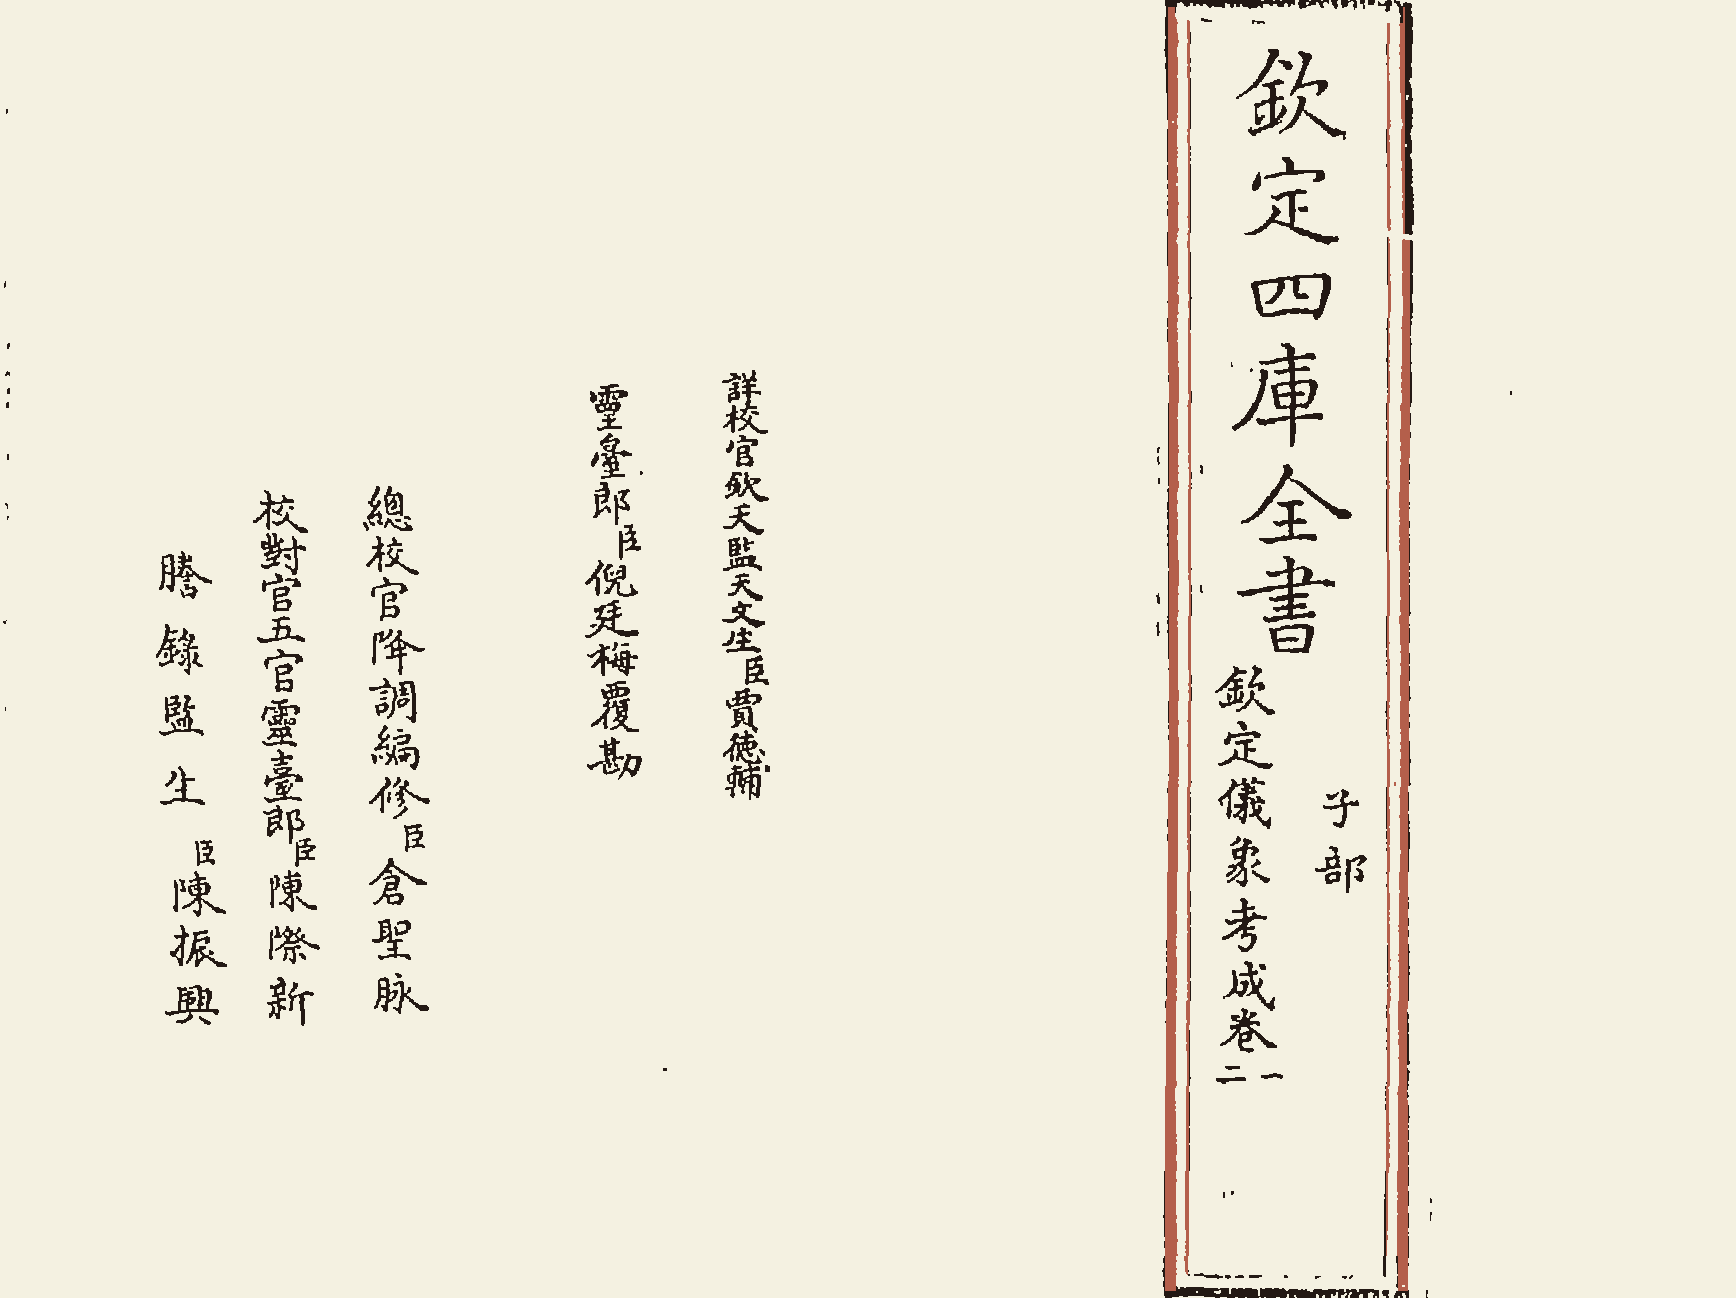
\includegraphics[width=\paperwidth,height=\paperheight,keepaspectratio]{img/0400.png}\clearpage
\begin{正文}
% ---- 册793 葉401 ----
\SetPageNumber{1}
欽定四庫全書\换行
欽定儀象考成卷一\换行
　恒星總紀\换行
　　三垣\换行
　　一十八宿\换行
　　恒星全圖\换行
　　赤道北恒星圖\换行
　　赤道南恒星圖\换行
\char"200B\relax\换行
\char"200B\relax\换行
\char"200B\relax\换行
\char"200B\relax\换行
\char"200B\relax\换行
\char"200B\relax\换行
\char"200B\relax\换行
\char"200B\relax
\par
% ---- 册793 葉404 ----
　　恒星總紀\换行
恒星即經星也以其有常不易故名經星\双列{\右小列{史記天官書}\左小列{紫宫房心權}}\换行
\双列{\右小列{衡咸池虚危列宿部星此天之五宫坐}\左小列{位也為經不移徙大小有差濶狹有常}}經星又各有經\换行
緯度故别之曰恒星其星官名數古今不同漢書天文\换行
志經星常宿中外官凡百一十八名積數七百八十三\换行
星晉志載呉太史令陳卓始列甘石巫咸三家星官著\换行
於圖録凡二百八十三官一千四百六十四星今皆不\换行
見原本隋丹元子歩天歌與陳卓數合後此言天官者\换行
皆以歩天歌為凖康熙十三年監臣南懐仁修儀象志\换行
星名與古同者總二百五十九座一千一百二十九星\换行
比歩天歌少二十四座三百三十五星又於有名常數\换行
之外増五百九十七星又多近南極星二十三座一百\换行
五十星近年以來累加測騐星官度數儀象志尚多未\换行
合又星之次第多不順序亦宜釐正於是逐星測量推\换行
其度數觀其形象序其次第著之於圖計三垣二十八\换行
宿星名與古同者總二百七十七座一千三百一十九
\par
% ---- 册793 葉405 ----
星比儀象志多十八座一百九十星與歩天歌為近其\换行
尤與古合者二十八宿次舍自古皆觜宿在前參宿在\换行
後其以何星作距古無明文唐書云古以參右肩為距\换行
失之太逺文獻通考載宋兩朝天文志云觜三星距西\换行
南星參十星距中星西第一星西法觜宿距中上星參\换行
宿亦距中西一星今按觜宿中上星在西南星前僅六\换行
分餘而西南星小中上星大則以中上星作距可也若\换行
參宿以中西一星作距星則觜宿之黄道度已在參宿\换行
後一度餘即赤道度亦在參宿後三十一分餘今依次\换行
順序以參宿中三星之東一星作距星則觜宿黄道度\换行
恒在參前一度弱與觜前參後之序合其餘諸座之星\换行
皆以次順序無凌躐顛倒之弊又於有名常數之外増\换行
一千六百一十四星近某座者即名某座増星依次分\换行
註方位以備稽考其近南極星二十三座一百五十星\换行
中國所不見仍依西測之舊共計恒星三百座三千八\换行
十三星編為總紀一卷庶星官名數古今不同及黄道
\par
% ---- 册793 葉408 ----
赤道所屬宫次皆展卷瞭然矣\换行
\char"200B\relax\换行
\char"200B\relax\换行
\char"200B\relax\换行
\char"200B\relax\换行
\char"200B\relax\换行
\char"200B\relax\换行
\char"200B\relax\换行
\char"200B\relax\换行
\char"200B\relax\换行
\char"200B\relax\换行
\char"200B\relax\换行
\char"200B\relax\换行
\char"200B\relax\换行
\char"200B\relax\换行
\char"200B\relax
\par
% ---- 册793 葉409 ----
紫微垣\换行
北極五星一太子二帝星三庶子四后宫五天樞外庶\换行
子増三星后宫増一星黄道在午未宫赤道在卯辰宫\换行
四輔四星外増一星黄道在未宫赤道在已午宫\换行
勾陳六星外増十星黄道在未申宫赤道在丑寅卯戌\换行
亥宫\换行
天皇大帝一星黄道在申宫赤道在亥宫\换行
天柱五星外増六星黄道在申酉宫赤道在子丑宫\换行
御女四星外増一星黄道在未申酉宫赤道在丑寅宫\换行
女史一星外増一星黄道在未宫赤道在寅宫\换行
柱史一星外増二星黄道在申宫赤道在丑宫\换行
尚書五星外増二星黄道在辰已午宫赤道在寅宫\换行
天床六星外増一星黄道在巳午宫赤道在寅卯宫\换行
大理二星外増一星黄道在未宫赤道在辰巳宫\换行
陰德二星外増一星黄道在未宫赤道在巳宫\换行
六甲六星外増一星黄道赤道俱在未申宫
\par
% ---- 册793 葉412 ----
五帝内座五星外増二星黄道在申宫赤道在酉戌宫\换行
華葢七星黄道在酉宫赤道在戌宫\换行
杠九星附華葢為一座外増一星黄道在申酉宫赤道\换行
在酉戌宫\换行
右垣墻七星一右樞二少尉三上輔四少輔五上衛六\换行
少衛七上丞外少尉増二星上輔増二星少輔増一星\换行
上衛増三星少衛増一星上丞増三星黄道在已午未\换行
申宫赤道在辰已午未申酉宫\换行
左垣墻八星一左樞二上宰三少宰四上弼五少弼六\换行
上衛七少衛八少丞外上衛増三星少衛増八星少丞\换行
増一星黄道在辰已酉宫赤道在戌亥子丑寅卯宫\换行
天乙一星黄道在已宫赤道在辰宫\换行
太乙一星黄道在午宫赤道在辰宫\换行
内厨二星外増二星黄道在午宫赤道在辰宫\换行
北斗七星一天樞二天璇三天璣四天權五玉衡六開\换行
陽七揺光外天樞増三星天璇増八星天權増三星開
\par
% ---- 册793 葉413 ----
陽増二星黄道在已午宫赤道在辰已宫\换行
輔一星附北斗為一座外増三星黄道在已宫赤道在\换行
辰宫\换行
天槍三星外増四星黄道在已宫赤道在卯宫\换行
元戈一星外増二星黄道在辰宫赤道在卯宫\换行
三公三星黄道在已宫赤道在辰宫\换行
相一星外増三星黄道在已宫赤道在辰宫\换行
天理四星外増一星黄道在午宫赤道在已宫\换行
太陽守一星外増一星黄道赤道俱在巳宫\换行
太尊一星黄道在午宫赤道在巳宫\换行
天牢六星外増二星黄道在巳午宫赤道在巳宫\换行
勢四星外増十六星黄道在午宫赤道在巳宫\换行
文昌六星外増八星黄道在午未宫赤道在午宫\换行
内階六星外増十星黄道在未宫赤道在午宫\换行
三師三星外増一星黄道在未宫赤道在午宫\换行
八榖八星外増三十四星黄道赤道俱在申宫
\par
% ---- 册793 葉416 ----
傳舍九星外増四星黄道在申酉宫赤道在酉戌亥宫\换行
天厨六星外増二星黄道在戌宫赤道在子丑宫\换行
天棓五星外増十星黄道赤道俱在寅宫\换行
　右共三十七座一百六十三星外増一百七十七星\换行
太微垣\换行
五帝座五星外増三星黄道赤道俱在巳宫\换行
太子一星黄道赤道俱在巳宫\换行
從官一星黄道赤道俱在巳宫\换行
幸臣一星黄道赤道俱在巳宫\换行
五諸侯五星外増七星黄道在辰巳宫赤道在辰宫\换行
九卿三星外増九星黄道赤道俱在辰宫\换行
三公三星黄道赤道俱在辰宫\换行
内屏四星外増六星黄道赤道俱在巳宫\换行
右垣墻五星一右執法二上將三次將四次相五上相\换行
外次相増三星上相増二星黄道赤道俱在巳宫\换行
左垣墻五星一左執法二上相三次相四次將五上將
\par
% ---- 册793 葉417 ----
外左執法增一星次相増一星次將増三星上將増二\换行
星黄道赤道俱在辰宫\换行
郎將一星外増二星黄道在巳宫赤道在辰宫\换行
郎位十五星外増三星黄道在巳宫赤道在辰巳宫\换行
常陳七星外増六星黄道在巳宫赤道在辰巳宫\换行
三台六星上台二星中台二星下台二星外上台増七\换行
星中台増三星下台増二星黄道在巳午未宫赤道在\换行
巳午宫\换行
虎賁一星黄道赤道俱在巳宫\换行
少微四星外增八星黄道在巳午宫赤道在巳宫\换行
長垣四星外増九星黄道在巳午宫赤道在巳宫\换行
靈臺三星外増八星黄道赤道俱在巳宫\换行
明堂三星外増六星黄道赤道俱在巳宫\换行
謁者一星外増二星黄道在巳宫赤道在辰宫\换行
　右共二十座七十八星外増九十三星\换行
天市垣
\par
% ---- 册793 葉420 ----
帝座一星黄道赤道俱在寅宫\换行
候一星外増五星黄道赤道俱在寅宫\换行
宦者四星外増五星黄道赤道俱在寅宫\换行
斗五星外増十四星黄道在寅卯宫赤道在寅宫\换行
斛四星外増三星黄道赤道俱在寅宫\换行
列肆二星外増四星黄道在寅卯宫赤道在寅宫\换行
車肆二星外増二星黄道赤道俱在寅宫\换行
市樓六星外増一星黄道赤道俱在寅宫\换行
宗正二星外増三星黄道赤道俱在寅宫\换行
宗人四星外増四星黄道赤道俱在寅宫\换行
宗二星黄道赤道俱在丑宫\换行
帛度二星外増三星黄道赤道俱在寅宫\换行
屠肆二星外増三星黄道赤道俱在丑寅宫\换行
右垣墻十一星一河中二河間三晉四鄭五周六秦七\换行
蜀八巴九梁十楚十一韓外河間増一星晉増三星周\换行
増十四星秦増一星蜀増二星巴増四星黄道赤道俱
\par
% ---- 册793 葉421 ----
在寅卯宫\换行
左垣墻十一星一魏二趙三九河四中山五齊六呉越\换行
七徐八東海九燕十南海十一宋外魏増八星趙増三\换行
星九河増一星中山増七星齊増八星呉越増七星徐\换行
増四星東海増四星宋増二星黄道赤道俱在丑寅宫\换行
天紀九星外増十四星黄道在寅卯宫赤道在寅宫\换行
女牀三星黄道赤道俱在寅宫\换行
貫索九星外増十三星黄道赤道俱在卯宫\换行
七公七星外増十六星黄道在卯辰宫赤道在寅卯宫\换行
　右共十九座八十七星外増一百五十九星\换行
角宿\换行
角宿二星外増十五星黄道赤道俱在辰宫\换行
平道二星黄道赤道俱在辰宫\换行
天田二星外増六星黄道赤道俱在辰宫\换行
周鼎三星黄道在辰巳宫赤道在辰宫\换行
進賢一星外増九星黄道赤道俱在辰宫
\par
% ---- 册793 葉424 ----
天門二星外増十一星黄道赤道俱在辰宫\换行
平二星外増三星黄道在卯辰宫赤道在辰宫\换行
庫樓十星外増一星黄道赤道俱在卯辰宫\换行
柱十一星黄道赤道俱在卯辰宫\换行
衡四星黄道在卯宫赤道在辰宫\换行
南門二星外増二星黄道在卯宫赤道在卯辰宫\换行
　右共十一座四十一星外増四十七星\换行
亢宿\换行
亢宿四星外増十二星黄道在卯宫赤道在卯辰宫\换行
大角一星外増一星黄道在辰宫赤道在卯宫\换行
右攝提三星外増三星黄道赤道俱在辰宫\换行
左攝提三星外増三星黄道在卯辰宫赤道在卯宫\换行
折威七星外増六星黄道赤道俱在卯宫\换行
頓頑二星外増一星黄道赤道俱在卯宫\换行
陽門二星黄道赤道俱在卯宫\换行
　右共七座二十二星外増二十六星
\par
% ---- 册793 葉425 ----
氐宿\换行
氐宿四星外増二十九星黄道赤道俱在卯宫\换行
亢池四星黄道在辰宫赤道在卯辰宫\换行
帝席三星外増一星黄道赤道俱在辰宫\换行
梗河三星外増五星黄道在卯辰宫赤道在卯宫\换行
招揺一星黄道在辰宫赤道在卯宫\换行
天乳一星外増三星黄道赤道俱在卯宫\换行
天輻二星外増一星黄道赤道俱在卯宫\换行
陣車三星外増二星黄道赤道俱在卯宫\换行
騎官十星黄道赤道俱在卯宫\换行
車騎三星黄道赤道俱在卯宫\换行
將軍一星黄道赤道俱在卯宫\换行
　右共十一座三十五星外増四十一星\换行
房宿\换行
房宿四星外増六星黄道赤道俱在卯宫\换行
鈎鈐二星附房宿為一座黄道在寅宫赤道在卯宫
\par
% ---- 册793 葉428 ----
鍵閉一星黄道在卯宫赤道在寅宫\换行
罰三星外増三星黄道在卯宫赤道在寅卯宫\换行
西咸四星外増二星黄道赤道俱在卯宫\换行
東咸四星外増一星黄道赤道俱在寅宫\换行
日一星外増一星黄道赤道俱在卯宫\换行
從官二星外増一星黄道赤道俱在卯宫\换行
　右共七座二十一星外増十四星\换行
心宿\换行
心宿三星外増八星黄道赤道俱在寅宫\换行
積卒二星黄道在寅宫赤道在卯宫\换行
　右共二座五星外増八星\换行
尾宿\换行
尾宿九星外増一星黄道赤道俱在寅宫\换行
神宫一星附尾宿為一座黄道赤道俱在寅宫\换行
天江四星外増十一星黄道赤道俱在寅宫\换行
傅説一星黄道赤道俱在寅宫
\par
% ---- 册793 葉429 ----
魚一星黄道赤道俱在寅宫\换行
龜五星黄道赤道俱在寅宫\换行
　右共五座二十一星外増十二星\换行
箕宿\换行
箕宿四星黄道赤道俱在丑寅宫\换行
糠一星黄道赤道俱在寅宫\换行
杵三星外増一星黄道赤道俱在寅宫\换行
　右共三座八星外増一星\换行
斗宿\换行
斗宿六星外増四星黄道赤道俱在丑寅宫\换行
天籥八星外増四星黄道赤道俱在寅宫\换行
天弁九星外増五星黄道赤道俱在丑宫\换行
建六星外増八星黄道赤道俱在丑宫\换行
天雞二星外増三星黄道赤道俱在丑宫\换行
狗二星外増六星黄道赤道俱在丑宫\换行
狗國四星黄道赤道俱在丑宫
\par
% ---- 册793 葉432 ----
天淵三星黄道赤道俱在丑宫\换行
農丈人一星黄道赤道俱在丑宫\换行
鼈十一星黄道赤道俱在丑宫\换行
　右共十座五十二星外増三十星\换行
牛宿\换行
牛宿六星外増九星黄道赤道俱在子丑宫\换行
天桴四星外増二星黄道在子丑宫赤道在丑宫\换行
河鼓三星外増九星黄道赤道俱在丑宫\换行
右旗九星外増十二星黄道赤道俱在丑宫\换行
左旗九星外増二十九星黄道赤道俱在子丑宫\换行
織女三星外増四星黄道赤道俱在丑宫\换行
漸臺四星外増六星黄道赤道俱在丑宫\换行
輦道五星外増九星黄道在子丑宫赤道在丑宫\换行
羅堰三星外增一星黄道赤道俱在子宫\换行
天田四星黄道赤道俱在子宫\换行
九坎四星黄道赤道俱在子宫
\par
% ---- 册793 葉433 ----
　右共十一座五十四星外増八十一星\换行
女宿\换行
女宿四星外増五星黄道赤道俱在子宫\换行
離珠四星外増一星黄道赤道俱在子宫\换行
敗𤓰五星外増三星黄道赤道俱在子宫\换行
瓠𤓰五星外増五星黄道赤道俱在子宫\换行
天津九星外増三十八星黄道在亥子宫赤道在子丑\换行
宫\换行
奚仲四星外増七星黄道在子宫赤道在丑宫\换行
扶筐七星外増四星黄道在子丑宫赤道在丑宫\换行
十二國十六星周二星秦二星代二星趙二星越一星\换行
齊一星楚一星鄭一星魏一星韓一星晉一星燕一星\换行
外代増二星黄道赤道俱在子宫\换行
　右共八座五十四星外増六十五星\换行
虚宿\换行
虚宿二星外増八星黄道赤道俱在子宫
\par
% ---- 册793 葉436 ----
司命二星黄道赤道俱在子宫\换行
司禄二星外増二星黄道赤道俱在子宫\换行
司危二星黄道赤道俱在子宫\换行
司非二星外増二星黄道赤道俱在子宫\换行
哭二星外増四星黄道赤道俱在子宫\换行
泣二星外増二星黄道在亥子宫赤道在亥宫\换行
離瑜三星外増三星黄道赤道俱在子宫\换行
天壘城十三星黄道赤道俱在子宫\换行
敗臼四星外増一星黄道在子宫赤道在亥子宫\换行
　右共十座三十四星外増二十二星\换行
危宿\换行
危宿三星外増十一星黄道在亥子宫赤道在子宫\换行
墳墓四星附危宿為一座外増四星黄道赤道俱在亥\换行
宫\换行
葢屋二星黄道赤道俱在子宫\换行
虚梁四星黄道赤道俱在亥宫
\par
% ---- 册793 葉437 ----
天錢五星外増四星黄道赤道俱在子宫\换行
人四星外増四星黄道在亥子宫赤道在子宫\换行
杵三星外増二星黄道在亥宫赤道在亥子宫\换行
臼四星外増五星黄道在亥宫赤道在亥子宫\换行
車府七星外増十九星黄道在戌亥宫赤道在亥子宫\换行
造父五星外増五星黄道在戌宫赤道在亥子宫\换行
天鉤九星外増十六星黄道在酉戌宫赤道在亥子宫\换行
　右共十座五十星外増七十星\换行
室宿\换行
室宿二星外増七星黄道赤道俱在亥宫\换行
離宫六星附室宿為一座外増八星黄道赤道俱在亥\换行
宫\换行
螣蛇二十二星外増十四星黄道在戌亥宫赤道在亥\换行
子宫\换行
雷電六星外増八星黄道赤道俱在亥宫\换行
土公吏二星黄道赤道俱在亥宫
\par
% ---- 册793 葉440 ----
壘壁陣十二星外増七星黄道赤道俱在亥子宫\换行
羽林軍四十五星黄道赤道俱在亥子宫\换行
天綱一星黄道在子宫赤道在亥宫\换行
北落師門一星黄道赤道俱在亥宫\换行
鈇鉞三星外増二星黄道赤道俱在亥宫\换行
八魁六星黄道在亥宫赤道在戌亥宫\换行
　右共十座一百零六星外増四十六星\换行
壁宿\换行
壁宿二星外増二十三星黄道在戌宫赤道在戌亥宫\换行
天廐三星外増一星黄道赤道俱在戌宫\换行
土公二星外増十一星黄道在戌宫赤道在戌亥宫\换行
霹𩆝五星外増八星黄道赤道俱在亥宫\换行
雲雨四星外増九星黄道赤道俱在亥宫\换行
鈇鑕五星黄道赤道俱在戌宫\换行
　右共六座二十一星外増五十二星\换行
奎宿
\par
% ---- 册793 葉441 ----
奎宿十六星外増二十二星黄道赤道俱在戌宫\换行
王良五星外増五星黄道在酉宫赤道在戌亥宫\换行
䇿一星黄道在酉宫赤道在戌宫\换行
附路一星黄道在酉宫赤道在戌宫\换行
軍南門一星黄道在酉宫赤道在戌宫\换行
閣道六星外増五星黄道赤道俱在酉戌宫\换行
外屏七星外増十五星黄道赤道俱在戌宫\换行
天溷四星外増六星黄道赤道俱在戌宫\换行
土司空一星黄道在亥宫赤道在戌宫\换行
　右共九座四十二星外増五十三星\换行
婁宿\换行
婁宿三星外増十五星黄道在酉戌宫赤道在戌宫\换行
天大將軍十一星外増十六星黄道在酉宫赤道在酉\换行
戌宫\换行
右更五星外増五星黄道赤道俱在戌宫\换行
左更五星外増七星黄道赤道俱在酉宫
\par
% ---- 册793 葉444 ----
天倉六星外増十八星黄道在戌亥宫赤道在戌宫\换行
天庾三星外増三星黄道在戌宫赤道在酉戌宫\换行
　右共六座三十三星外増六十四星\换行
胃宿\换行
胃宿三星外増五星黄道赤道俱在酉宫\换行
大陵八星外増二十星黄道赤道俱在酉宫\换行
積尸一星黄道赤道俱在酉宫\换行
天船九星外増九星黄道在申酉宫赤道在酉宫\换行
積水一星外増一星黄道在申宫赤道在酉宫\换行
天廩四星外増二星黄道赤道俱在酉宫\换行
天囷十三星外増二十星黄道赤道俱在酉戌宫\换行
　右共七座三十九星外増五十七星\换行
昴宿\换行
昴宿七星外増五星黄道赤道俱在酉宫\换行
天阿一星黄道赤道俱在酉宫\换行
月一星外増一星黄道赤道俱在酉宫
\par
% ---- 册793 葉445 ----
卷舌六星外増六星黄道在申酉宫赤道在酉宫\换行
天讒一星黄道赤道俱在酉宫\换行
礪石四星黄道在申宫赤道在申酉宫\换行
天陰五星外増四星黄道赤道俱在酉宫\换行
蒭藁六星外増五星黄道在戌宫赤道在酉宫\换行
天苑十六星外増十六星黄道在酉戌宫赤道在酉宫\换行
　右共九座四十七星外増三十七星\换行
畢宿\换行
畢宿八星外増十三星黄道赤道俱在申酉宫\换行
附耳一星附畢宿為一座外増一星黄道赤道俱在申\换行
宫\换行
天街二星外増四星黄道赤道俱在申宫\换行
天髙四星外増四星黄道赤道俱在申宫\换行
諸王六星外増四星黄道赤道俱在申宫\换行
五車五星外増十八星黄道赤道俱在申宫\换行
柱九星黄道赤道俱在申宫
\par
% ---- 册793 葉448 ----
咸池三星黄道赤道俱在申宫\换行
天潢五星外増二星黄道赤道俱在申宫\换行
天闗一星外増六星黄道赤道俱在申宫\换行
天節八星黄道赤道俱在申宫\换行
九州殊口六星外増十星黄道赤道俱在申酉宫\换行
參旗九星外増十一星黄道赤道俱在申宫\换行
九斿九星外増五星黄道赤道俱在申宫\换行
天園十三星外増六星黄道在酉戌亥宫赤道在申酉\换行
戌宫\换行
　右共十四座八十九星外増八十四星\换行
觜宿\换行
觜宿三星黄道赤道俱在申宫\换行
司怪四星外増六星黄道赤道俱在申宫\换行
座旗九星外増十一星黄道赤道俱在未宫\换行
　右共三座十六星外増十七星\换行
參宿
\par
% ---- 册793 葉449 ----
參宿七星外増三十七星黄道赤道俱在申宫\换行
伐三星附參宿為一座外増二星黄道赤道俱在申宫\换行
玉井四星外増二星黄道赤道俱在申宫\换行
軍井四星外増一星黄道赤道俱在申宫\换行
屏二星黄道赤道俱在申宫\换行
厠四星外増七星黄道赤道俱在申宫\换行
屎一星黄道赤道俱在申宫\换行
　右共六座二十五星外増四十九星\换行
井宿\换行
井宿八星外増十七星黄道赤道俱在未宫\换行
龯一星附井宿為一座外増一星黄道赤道俱在申宫\换行
水府四星外増八星黄道赤道俱在未申宫\换行
天罇三星外増九星黄道赤道俱在未宫\换行
五諸侯五星外増五星黄道赤道俱在未宫\换行
北河三星外増四星黄道赤道俱在未宫\换行
積水一星黄道赤道俱在未宫
\par
% ---- 册793 葉452 ----
積薪一星外増三星黄道赤道俱在未宫\换行
水位四星外増十一星黄道赤道俱在未宫\换行
南河三星外増十星黄道赤道俱在未宫\换行
四瀆四星外増六星黄道赤道俱在未宫\换行
闕邱二星外増七星黄道赤道俱在未宫\换行
軍市六星外増五星黄道赤道俱在未宫\换行
野雞一星黄道赤道俱在未宫\换行
天狼一星外増五星黄道赤道俱在未宫\换行
丈人二星黄道赤道俱在申宫\换行
子二星外増一星黄道赤道俱在申宫\换行
孫二星外増四星黄道赤道俱在未申宫\换行
老人一星外増四星黄道赤道俱在未宫\换行
弧矢九星外増二十四星黄道在午未宫赤道在未宫\换行
　右共十九座六十三星外増一百二十四星\换行
鬼宿\换行
鬼宿四星外増十八星黄道赤道俱在午宫
\par
% ---- 册793 葉453 ----
積尸氣一星外増三星黄道赤道俱在午宫\换行
爟四星外増十一星黄道赤道俱在未宫\换行
外厨六星外増十七星黄道赤道俱在午宫\换行
天記一星外増二星黄道在己宫赤道在午宫\换行
天狗七星黄道在巳午宫赤道在午宫\换行
天社六星外増五星黄道在辰巳午宫赤道在午宫\换行
　右共六座二十九星外増五十七星\换行
柳宿\换行
柳宿八星外増十星黄道赤道俱在午宫\换行
酒旗三星外増五星黄道赤道俱在午宫\换行
　右共二座十一星外増十五星\换行
星宿\换行
星宿七星外増十五星黄道赤道俱在午宫\换行
天相三星外増十二星黄道在己宫赤道在己午宫\换行
軒轅十七星外増五十七星黄道赤道俱在己午宫\换行
内平四星外増十一星黄道在午宫赤道在己午宫
\par
% ---- 册793 葉456 ----
　右共四座三十一星外増九十五星\换行
張宿\换行
張宿六星外増四星黄道赤道俱在己午宫\换行
　右一座六星外増四星\换行
翼宿\换行
翼宿二十二星外增七星黄道在辰己宫赤道在己宫\换行
　右一座二十二星外増七星\换行
軫宿\换行
軫宿四星外増五星黄道在辰宫赤道在辰己宫\换行
右轄一星附軫宿為一座黄道在辰宫赤道在己宫\换行
左轄一星附軫宿為一座黄道赤道俱在辰宫\换行
長沙一星附軫宿為一座黄道赤道俱在辰宫\换行
青邱七星外増三星黄道在辰宫赤道在己宫\换行
　右共二座十四星外増八星\换行
　總計三垣二十八宿共二百七十七座一千三百一\换行
　十九星外増一千六百一十四星按天文歩天歌角
\par
% ---- 册793 葉457 ----
　宿内柱十五星今少四星氐宿内亢池六星今少二\换行
　星騎官二十七星今少十七星心宿内積卒十二星\换行
　今少十星斗宿内天淵十星今少七星鼈十四星今\换行
　少三星牛宿内天田九星今少五星九坎九星今少\换行
　五星女宿内離珠五星今少一星危宿内天錢十星\换行
　今少五星人五星今少一星室宿内八魁九星今少\换行
　三星壁宿内天廐十星今少七星奎宿内天溷七星\换行
　今少三星畢宿内九州殊口九星今少三星井宿内\换行
　軍市十三星今少七星共少八十三星星宿内天稷\换行
　五星張宿内天廟十四星翼宿内東甌五星軫宿内\换行
　軍門二星土司空四星器府三十二星共六座六十\换行
　二星今無\换行
近南極星\换行
海山六星外増二星黄道在卯辰宫赤道在己宫\换行
十字四星黄道在卯宫赤道在辰宫\换行
馬尾三星黄道在辰宫赤道在辰己宫
\par
% ---- 册793 葉460 ----
馬腹三星黄道在卯宫赤道在辰宫\换行
蜜蜂四星黄道在卯宫赤道在辰宫\换行
三角形三星外増四星黄道在寅宫赤道在寅卯宫\换行
異雀九星黄道在寅宫赤道在寅卯辰宫\换行
孔雀十一星外増四星黄道在丑寅宫赤道在子丑寅\换行
宫\换行
波斯十一星黄道赤道俱在子丑宫\换行
蛇尾四星黄道在丑宫赤道在戌亥子宫\换行
蛇腹四星黄道在亥子宫赤道在酉戌宫\换行
蛇首二星黄道在亥宫赤道在酉戌宫\换行
鳥喙七星外増一星黄道在子宫赤道在戌亥宫\换行
鶴十二星外増二星黄道在子宫赤道在亥子宫\换行
火鳥十星外増一星黄道在亥子宫赤道在戌亥宫\换行
水委三星黄道在亥宫赤道在戌宫\换行
附白二星黄道在子宫赤道在酉宫\换行
夾白二星黄道在戌亥宫赤道在申酉宫
\par
% ---- 册793 葉461 ----
金魚五星外増一星黄道在寅酉戌宫赤道在未申宫\换行
海石五星外増三星黄道在辰己宫赤道在午宫\换行
飛魚六星黄道在卯辰宫赤道在午未宫\换行
南船五星外増一星黄道在卯辰宫赤道在己午宫\换行
小斗九星外増一星黄道在寅卯宫赤道在辰巳午未\换行
宫\换行
　右共二十三座一百三十星外増二十星古無\换行
\char"200B\relax\换行
\char"200B\relax\换行
\char"200B\relax\换行
\char"200B\relax\换行
\char"200B\relax\换行
\char"200B\relax\换行
\char"200B\relax\换行
\char"200B\relax\换行
\char"200B\relax
\par
% ---- 册793 葉464 ----
　　恒星全圖\换行
唐書天文志葢天之説一行削篾為度徑一分其厚半\换行
之長與圖等穴其正中植鍼為樞令可環運自中樞之\换行
外均刻百四十七度全度之末旋為外規規外大半度\换行
再旋為重規以均賦周天度分又距極樞九十一度少\换行
半旋為赤道𢃄天之紘距極三十五度旋為内規乃歩\换行
冬至日躔所在以正辰次之中以立宿距按渾儀所測\换行
甘石巫咸衆星明者皆以篾横考入宿距縱考去極度\换行
而後圖之其赤道外衆星踈宻之狀與仰視小殊者由\换行
渾儀去南極漸近其度益狹而葢圖漸逺其度益廣使\换行
然若考其去極入宿度數移之於渾天則一也又赤道\换行
内外其廣狹不均若就二至出入赤道二十四度以規\换行
度之則二分所交不得其正自二分黄赤道交以規度\换行
之則二至距極度數不得其正當求黄赤分至之中均\换行
刻為七十二限據每黄道差數以篾度量而識之然後\换行
規為黄道則周天咸得其正矣今按渾天係圓體圖之
\par
% ---- 册793 葉465 ----
於平面止見其半故渾天不可圖葢天圖以北極為中\换行
心乃見星座全象然其内外二規亦猶是渾天之法也\换行
渾天家以北極出地常見不隠謂之上規南極入地常\换行
隠不見謂之下規一行葢天圖以三十五度為内規即\换行
上規之度也\双列{\右小列{北極出地}\左小列{三十五度}}一百四十七度為外規即北極\换行
距下規之度也\双列{\右小列{古法周天三百六十五度四分度之一}\左小列{則北極距南極為一百八十二度有竒}}\换行
\双列{\右小列{除南極入地三十五度}\左小列{有竒餘一百四十七度}}今法周天三百六十度赤道距\换行
南北極各九十度京師北極出地四十度故以四十度\换行
為内規中國幅隕南至北極出地二十度則北極距下\换行
規一百六十度故以一百六十度為外規其餘悉如一\换行
行之法依新測恒星赤道經緯度著之於圖仍用赤黄\换行
黒三色以存三家之舊又以赤道南北分為二圖則北\换行
極出地二十度以南所見之星座無不備具雖中天所\换行
見星座横分為二然赤道以南其度漸狹可以補葢天\换行
星度益廣之失合觀三圖則懸象著明躔離攸次星之\换行
隠見天漢昭回庶幾無遺憾矣
\par
\end{正文}\clearpage
\嵌图{141.61pt}{202.05pt}{848.55pt}{585.69pt}{img/0470.png}
\begin{正文}
% ---- 册793 葉470 图版 ----
\SetPageNumber{34}
\插图页
\char"200B\relax\换行
\char"200B\relax\换行
\char"200B\relax\换行
\char"200B\relax\换行
\char"200B\relax\换行
\char"200B\relax\换行
\char"200B\relax\换行
\char"200B\relax\换行
\char"200B\relax\换行
\char"200B\relax\换行
\char"200B\relax\换行
\char"200B\relax\换行
\char"200B\relax\换行
\char"200B\relax\换行
\char"200B\relax\换行
\char"200B\relax
\恢复丝栏\par
\end{正文}\clearpage
\嵌图{145.79pt}{200.67pt}{840.19pt}{588.45pt}{img/0474.png}
\begin{正文}
% ---- 册793 葉474 图版 ----
\SetPageNumber{35}
\插图页
\char"200B\relax\换行
\char"200B\relax\换行
\char"200B\relax\换行
\char"200B\relax\换行
\char"200B\relax\换行
\char"200B\relax\换行
\char"200B\relax\换行
\char"200B\relax\换行
\char"200B\relax\换行
\char"200B\relax\换行
\char"200B\relax\换行
\char"200B\relax\换行
\char"200B\relax\换行
\char"200B\relax\换行
\char"200B\relax\换行
\char"200B\relax
\恢复丝栏\par
\end{正文}\clearpage
\嵌图{147.13pt}{204.95pt}{837.49pt}{579.89pt}{img/0478.png}
\begin{正文}
% ---- 册793 葉478 图版 ----
\SetPageNumber{36}
\插图页
\char"200B\relax\换行
\char"200B\relax\换行
\char"200B\relax\换行
\char"200B\relax\换行
\char"200B\relax\换行
\char"200B\relax\换行
\char"200B\relax\换行
\char"200B\relax\换行
\char"200B\relax\换行
\char"200B\relax\换行
\char"200B\relax\换行
\char"200B\relax\换行
\char"200B\relax\换行
\char"200B\relax\换行
\char"200B\relax\换行
\char"200B\relax
\恢复丝栏\par

% ======== 卷二（8行21字）========
\par\end{正文}\clearpage
\chapter*{欽定儀象考成卷二}
\begin{正文}
% ---- 册793 葉480 ----
\SetPageNumber{1}
欽定四庫全書\换行
欽定儀象考成卷二\换行
　恒星黄道經緯度表一\换行
　　黄道星紀宫\双列{\右小列{赤道度附}\左小列{}}\换行
\char"200B\relax\换行
\char"200B\relax\换行
\char"200B\relax\换行
\char"200B\relax\换行
\char"200B\relax\换行
\char"200B\relax\换行
\char"200B\relax\换行
\char"200B\relax\换行
\char"200B\relax\换行
\char"200B\relax\换行
\char"200B\relax\换行
\char"200B\relax
\par
% ---- 册793 葉481 ----
　　恒星黄赤經緯度表\换行
恒星布列周天古有去極入宿度數入宿即經度也去\换行
極即緯度也然黄道度與赤道度不同嵗差亦異葢黄\换行
道以黄極為樞赤道以赤極為樞兩道兩極各相距二\换行
十三度半故星在兩極之間者黄道屬未宫赤道則屬\换行
丑宫星在兩道之間者黄道屬緯南赤道則屬緯北此\换行
黄赤不同之極致也恒星循黄道東行每年五十一秒\换行
緯度終古不改而經度之差有常赤道與黄道斜交分\换行
至前後南北逺近其差不等兩極之間在黄道為差而\换行
東在赤道為差而西兩交之際黄道南者差而入赤道\换行
北黄道北者差而出赤道南此嵗差不同之極致也今\换行
以乾隆九年甲子恒星黄赤經緯度依黄道次序列恒\换行
星黄道經緯度表而以赤道經緯附之依赤道次序列\换行
恒星赤道經緯度表而以黄道經緯附之各將赤道嵗\换行
差列於其下黄道以便推算赤道以便測量厯象之用\换行
於斯備矣
\par
\end{正文}\clearpage
\嵌图{142.64pt}{198.13pt}{846.47pt}{593.52pt}{img/0484.png}
\begin{正文}
% ---- 册793 葉484 图版 ----
\SetPageNumber{3}
\插图页
\char"200B\relax\换行
\char"200B\relax\换行
\char"200B\relax\换行
\char"200B\relax\换行
\char"200B\relax\换行
\char"200B\relax\换行
\char"200B\relax\换行
\char"200B\relax\换行
\char"200B\relax\换行
\char"200B\relax\换行
\char"200B\relax\换行
\char"200B\relax\换行
\char"200B\relax\换行
\char"200B\relax\换行
\char"200B\relax\换行
\char"200B\relax
\恢复丝栏\par
\end{正文}\clearpage
\嵌图{142.64pt}{198.61pt}{846.47pt}{592.57pt}{img/0485.png}
\begin{正文}
% ---- 册793 葉485 图版 ----
\SetPageNumber{4}
\插图页
\char"200B\relax\换行
\char"200B\relax\换行
\char"200B\relax\换行
\char"200B\relax\换行
\char"200B\relax\换行
\char"200B\relax\换行
\char"200B\relax\换行
\char"200B\relax\换行
\char"200B\relax\换行
\char"200B\relax\换行
\char"200B\relax\换行
\char"200B\relax\换行
\char"200B\relax\换行
\char"200B\relax\换行
\char"200B\relax\换行
\char"200B\relax
\恢复丝栏\par
\end{正文}\clearpage
\嵌图{144.63pt}{200.02pt}{842.50pt}{589.74pt}{img/0488.png}
\begin{正文}
% ---- 册793 葉488 图版 ----
\SetPageNumber{5}
\插图页
\char"200B\relax\换行
\char"200B\relax\换行
\char"200B\relax\换行
\char"200B\relax\换行
\char"200B\relax\换行
\char"200B\relax\换行
\char"200B\relax\换行
\char"200B\relax\换行
\char"200B\relax\换行
\char"200B\relax\换行
\char"200B\relax\换行
\char"200B\relax\换行
\char"200B\relax\换行
\char"200B\relax\换行
\char"200B\relax\换行
\char"200B\relax
\恢复丝栏\par
\end{正文}\clearpage
\嵌图{144.63pt}{200.00pt}{842.50pt}{589.78pt}{img/0489.png}
\begin{正文}
% ---- 册793 葉489 图版 ----
\SetPageNumber{6}
\插图页
\char"200B\relax\换行
\char"200B\relax\换行
\char"200B\relax\换行
\char"200B\relax\换行
\char"200B\relax\换行
\char"200B\relax\换行
\char"200B\relax\换行
\char"200B\relax\换行
\char"200B\relax\换行
\char"200B\relax\换行
\char"200B\relax\换行
\char"200B\relax\换行
\char"200B\relax\换行
\char"200B\relax\换行
\char"200B\relax\换行
\char"200B\relax
\恢复丝栏\par
\end{正文}\clearpage
\嵌图{148.54pt}{198.57pt}{834.68pt}{592.64pt}{img/0492.png}
\begin{正文}
% ---- 册793 葉492 图版 ----
\SetPageNumber{7}
\插图页
\char"200B\relax\换行
\char"200B\relax\换行
\char"200B\relax\换行
\char"200B\relax\换行
\char"200B\relax\换行
\char"200B\relax\换行
\char"200B\relax\换行
\char"200B\relax\换行
\char"200B\relax\换行
\char"200B\relax\换行
\char"200B\relax\换行
\char"200B\relax\换行
\char"200B\relax\换行
\char"200B\relax\换行
\char"200B\relax\换行
\char"200B\relax
\恢复丝栏\par
\end{正文}\clearpage
\嵌图{148.54pt}{197.60pt}{834.68pt}{594.58pt}{img/0493.png}
\begin{正文}
% ---- 册793 葉493 图版 ----
\SetPageNumber{8}
\插图页
\char"200B\relax\换行
\char"200B\relax\换行
\char"200B\relax\换行
\char"200B\relax\换行
\char"200B\relax\换行
\char"200B\relax\换行
\char"200B\relax\换行
\char"200B\relax\换行
\char"200B\relax\换行
\char"200B\relax\换行
\char"200B\relax\换行
\char"200B\relax\换行
\char"200B\relax\换行
\char"200B\relax\换行
\char"200B\relax\换行
\char"200B\relax
\恢复丝栏\par
\end{正文}\clearpage
\嵌图{148.61pt}{200.04pt}{834.55pt}{589.71pt}{img/0496.png}
\begin{正文}
% ---- 册793 葉496 图版 ----
\SetPageNumber{9}
\插图页
\char"200B\relax\换行
\char"200B\relax\换行
\char"200B\relax\换行
\char"200B\relax\换行
\char"200B\relax\换行
\char"200B\relax\换行
\char"200B\relax\换行
\char"200B\relax\换行
\char"200B\relax\换行
\char"200B\relax\换行
\char"200B\relax\换行
\char"200B\relax\换行
\char"200B\relax\换行
\char"200B\relax\换行
\char"200B\relax\换行
\char"200B\relax
\恢复丝栏\par
\end{正文}\clearpage
\嵌图{146.62pt}{199.56pt}{838.53pt}{590.67pt}{img/0497.png}
\begin{正文}
% ---- 册793 葉497 图版 ----
\SetPageNumber{10}
\插图页
\char"200B\relax\换行
\char"200B\relax\换行
\char"200B\relax\换行
\char"200B\relax\换行
\char"200B\relax\换行
\char"200B\relax\换行
\char"200B\relax\换行
\char"200B\relax\换行
\char"200B\relax\换行
\char"200B\relax\换行
\char"200B\relax\换行
\char"200B\relax\换行
\char"200B\relax\换行
\char"200B\relax\换行
\char"200B\relax\换行
\char"200B\relax
\恢复丝栏\par
\end{正文}\clearpage
\嵌图{142.64pt}{197.65pt}{846.47pt}{594.50pt}{img/0500.png}
\begin{正文}
% ---- 册793 葉500 图版 ----
\SetPageNumber{11}
\插图页
\char"200B\relax\换行
\char"200B\relax\换行
\char"200B\relax\换行
\char"200B\relax\换行
\char"200B\relax\换行
\char"200B\relax\换行
\char"200B\relax\换行
\char"200B\relax\换行
\char"200B\relax\换行
\char"200B\relax\换行
\char"200B\relax\换行
\char"200B\relax\换行
\char"200B\relax\换行
\char"200B\relax\换行
\char"200B\relax\换行
\char"200B\relax
\恢复丝栏\par
\end{正文}\clearpage
\嵌图{144.63pt}{199.49pt}{842.50pt}{590.81pt}{img/0501.png}
\begin{正文}
% ---- 册793 葉501 图版 ----
\SetPageNumber{12}
\插图页
\char"200B\relax\换行
\char"200B\relax\换行
\char"200B\relax\换行
\char"200B\relax\换行
\char"200B\relax\换行
\char"200B\relax\换行
\char"200B\relax\换行
\char"200B\relax\换行
\char"200B\relax\换行
\char"200B\relax\换行
\char"200B\relax\换行
\char"200B\relax\换行
\char"200B\relax\换行
\char"200B\relax\换行
\char"200B\relax\换行
\char"200B\relax
\恢复丝栏\par
\end{正文}\clearpage
\嵌图{144.68pt}{202.35pt}{842.41pt}{585.10pt}{img/0504.png}
\begin{正文}
% ---- 册793 葉504 图版 ----
\SetPageNumber{13}
\插图页
\char"200B\relax\换行
\char"200B\relax\换行
\char"200B\relax\换行
\char"200B\relax\换行
\char"200B\relax\换行
\char"200B\relax\换行
\char"200B\relax\换行
\char"200B\relax\换行
\char"200B\relax\换行
\char"200B\relax\换行
\char"200B\relax\换行
\char"200B\relax\换行
\char"200B\relax\换行
\char"200B\relax\换行
\char"200B\relax\换行
\char"200B\relax
\恢复丝栏\par
\end{正文}\clearpage
\嵌图{146.67pt}{202.84pt}{838.42pt}{584.11pt}{img/0505.png}
\begin{正文}
% ---- 册793 葉505 图版 ----
\SetPageNumber{14}
\插图页
\char"200B\relax\换行
\char"200B\relax\换行
\char"200B\relax\换行
\char"200B\relax\换行
\char"200B\relax\换行
\char"200B\relax\换行
\char"200B\relax\换行
\char"200B\relax\换行
\char"200B\relax\换行
\char"200B\relax\换行
\char"200B\relax\换行
\char"200B\relax\换行
\char"200B\relax\换行
\char"200B\relax\换行
\char"200B\relax\换行
\char"200B\relax
\恢复丝栏\par
\end{正文}\clearpage
\嵌图{144.72pt}{201.88pt}{842.31pt}{586.04pt}{img/0508.png}
\begin{正文}
% ---- 册793 葉508 图版 ----
\SetPageNumber{15}
\插图页
\char"200B\relax\换行
\char"200B\relax\换行
\char"200B\relax\换行
\char"200B\relax\换行
\char"200B\relax\换行
\char"200B\relax\换行
\char"200B\relax\换行
\char"200B\relax\换行
\char"200B\relax\换行
\char"200B\relax\换行
\char"200B\relax\换行
\char"200B\relax\换行
\char"200B\relax\换行
\char"200B\relax\换行
\char"200B\relax\换行
\char"200B\relax
\恢复丝栏\par
\end{正文}\clearpage
\嵌图{148.73pt}{202.36pt}{834.29pt}{585.07pt}{img/0509.png}
\begin{正文}
% ---- 册793 葉509 图版 ----
\SetPageNumber{16}
\插图页
\char"200B\relax\换行
\char"200B\relax\换行
\char"200B\relax\换行
\char"200B\relax\换行
\char"200B\relax\换行
\char"200B\relax\换行
\char"200B\relax\换行
\char"200B\relax\换行
\char"200B\relax\换行
\char"200B\relax\换行
\char"200B\relax\换行
\char"200B\relax\换行
\char"200B\relax\换行
\char"200B\relax\换行
\char"200B\relax\换行
\char"200B\relax
\恢复丝栏\par
\end{正文}\clearpage
\嵌图{144.63pt}{199.98pt}{842.50pt}{589.82pt}{img/0512.png}
\begin{正文}
% ---- 册793 葉512 图版 ----
\SetPageNumber{17}
\插图页
\char"200B\relax\换行
\char"200B\relax\换行
\char"200B\relax\换行
\char"200B\relax\换行
\char"200B\relax\换行
\char"200B\relax\换行
\char"200B\relax\换行
\char"200B\relax\换行
\char"200B\relax\换行
\char"200B\relax\换行
\char"200B\relax\换行
\char"200B\relax\换行
\char"200B\relax\换行
\char"200B\relax\换行
\char"200B\relax\换行
\char"200B\relax
\恢复丝栏\par
\end{正文}\clearpage
\嵌图{146.62pt}{201.36pt}{838.53pt}{587.07pt}{img/0513.png}
\begin{正文}
% ---- 册793 葉513 图版 ----
\SetPageNumber{18}
\插图页
\char"200B\relax\换行
\char"200B\relax\换行
\char"200B\relax\换行
\char"200B\relax\换行
\char"200B\relax\换行
\char"200B\relax\换行
\char"200B\relax\换行
\char"200B\relax\换行
\char"200B\relax\换行
\char"200B\relax\换行
\char"200B\relax\换行
\char"200B\relax\换行
\char"200B\relax\换行
\char"200B\relax\换行
\char"200B\relax\换行
\char"200B\relax
\恢复丝栏\par
\end{正文}\clearpage
\嵌图{167.87pt}{238.87pt}{125.06pt}{582.34pt}{img/0516.png}
\begin{正文}
% ---- 册793 葉516 ----
\SetPageNumber{19}
\char"200B\relax\换行
\char"200B\relax\换行
\char"200B\relax\换行
\char"200B\relax\换行
\char"200B\relax\换行
\char"200B\relax\换行
\char"200B\relax\换行
\char"200B\relax\换行
\char"200B\relax\换行
\char"200B\relax\换行
\char"200B\relax\换行
\char"200B\relax\换行
\char"200B\relax\换行
\char"200B\relax\换行
\char"200B\relax\换行
欽定儀象考成卷二
\par

\par\end{正文}\clearpage

  % ======== 卷三（8行21字）========
\chapter*{欽定儀象考成卷三}
\begin{正文}
\end{正文}\clearpage
\thispagestyle{empty}\noindent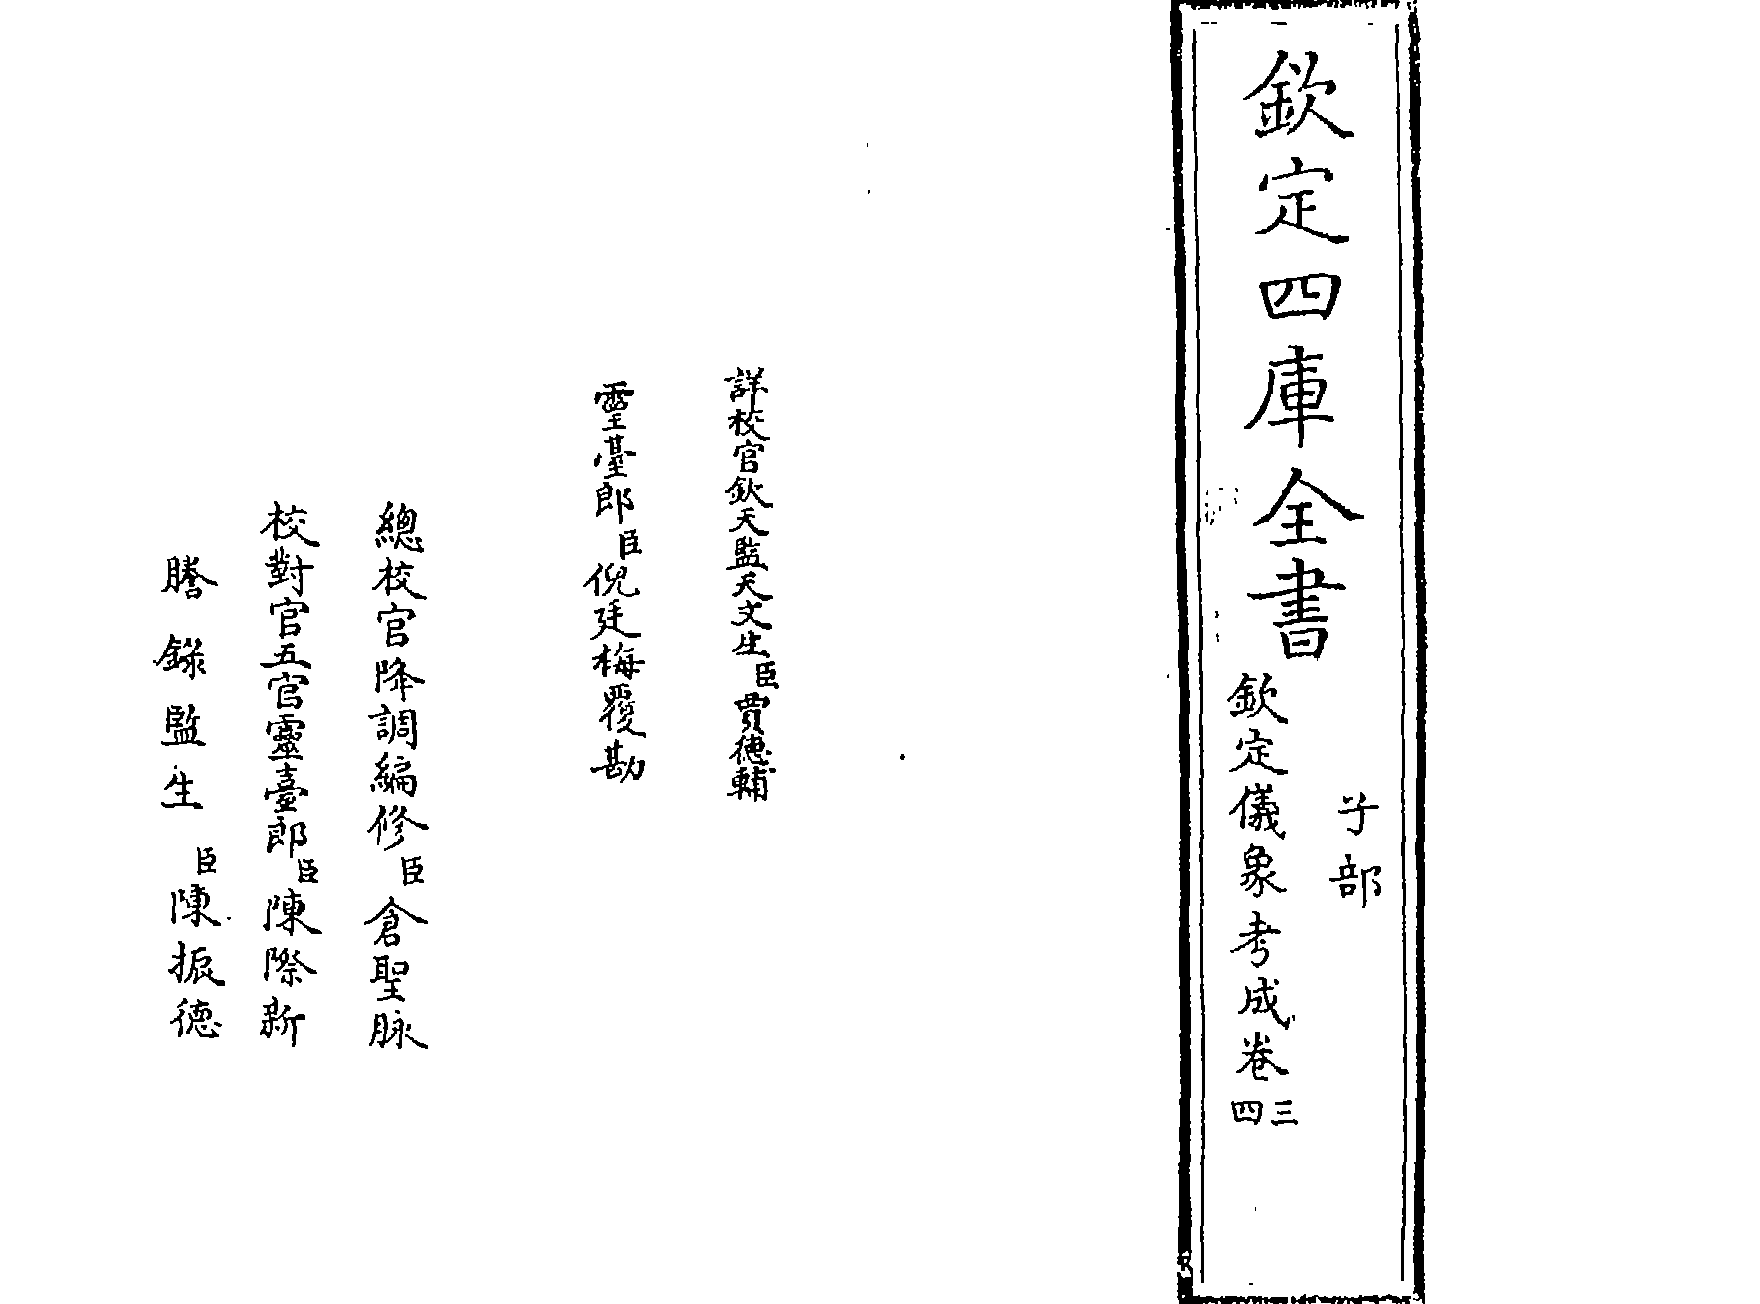
\includegraphics[width=\paperwidth,height=\paperheight,keepaspectratio]{img/0520.png}\clearpage
\begin{正文}
% ---- 册793 葉521 ----
\SetPageNumber{1}
欽定四庫全書\换行
欽定儀象考成卷三\换行
　恒星黄道經緯度表二\换行
　　黄道元枵宫\双列{\右小列{赤道度附}\左小列{}}\换行
\char"200B\relax\换行
\char"200B\relax\换行
\char"200B\relax\换行
\char"200B\relax\换行
\char"200B\relax\换行
\char"200B\relax\换行
\char"200B\relax\换行
\char"200B\relax\换行
\char"200B\relax\换行
\char"200B\relax\换行
\char"200B\relax\换行
\char"200B\relax
\par
\end{正文}\clearpage
\嵌图{142.64pt}{198.62pt}{846.47pt}{592.55pt}{img/0524.png}
\begin{正文}
% ---- 册793 葉524 图版 ----
\SetPageNumber{2}
\插图页
\char"200B\relax\换行
\char"200B\relax\换行
\char"200B\relax\换行
\char"200B\relax\换行
\char"200B\relax\换行
\char"200B\relax\换行
\char"200B\relax\换行
\char"200B\relax\换行
\char"200B\relax\换行
\char"200B\relax\换行
\char"200B\relax\换行
\char"200B\relax\换行
\char"200B\relax\换行
\char"200B\relax\换行
\char"200B\relax\换行
\char"200B\relax
\恢复丝栏\par
\end{正文}\clearpage
\嵌图{144.63pt}{197.19pt}{842.50pt}{595.40pt}{img/0525.png}
\begin{正文}
% ---- 册793 葉525 图版 ----
\SetPageNumber{3}
\插图页
\char"200B\relax\换行
\char"200B\relax\换行
\char"200B\relax\换行
\char"200B\relax\换行
\char"200B\relax\换行
\char"200B\relax\换行
\char"200B\relax\换行
\char"200B\relax\换行
\char"200B\relax\换行
\char"200B\relax\换行
\char"200B\relax\换行
\char"200B\relax\换行
\char"200B\relax\换行
\char"200B\relax\换行
\char"200B\relax\换行
\char"200B\relax
\恢复丝栏\par
\end{正文}\clearpage
\嵌图{142.68pt}{200.11pt}{846.40pt}{589.58pt}{img/0528.png}
\begin{正文}
% ---- 册793 葉528 图版 ----
\SetPageNumber{4}
\插图页
\char"200B\relax\换行
\char"200B\relax\换行
\char"200B\relax\换行
\char"200B\relax\换行
\char"200B\relax\换行
\char"200B\relax\换行
\char"200B\relax\换行
\char"200B\relax\换行
\char"200B\relax\换行
\char"200B\relax\换行
\char"200B\relax\换行
\char"200B\relax\换行
\char"200B\relax\换行
\char"200B\relax\换行
\char"200B\relax\换行
\char"200B\relax
\恢复丝栏\par
\end{正文}\clearpage
\嵌图{144.68pt}{202.93pt}{842.41pt}{583.94pt}{img/0529.png}
\begin{正文}
% ---- 册793 葉529 图版 ----
\SetPageNumber{5}
\插图页
\char"200B\relax\换行
\char"200B\relax\换行
\char"200B\relax\换行
\char"200B\relax\换行
\char"200B\relax\换行
\char"200B\relax\换行
\char"200B\relax\换行
\char"200B\relax\换行
\char"200B\relax\换行
\char"200B\relax\换行
\char"200B\relax\换行
\char"200B\relax\换行
\char"200B\relax\换行
\char"200B\relax\换行
\char"200B\relax\换行
\char"200B\relax
\恢复丝栏\par
\end{正文}\clearpage
\嵌图{144.63pt}{202.38pt}{842.50pt}{585.03pt}{img/0532.png}
\begin{正文}
% ---- 册793 葉532 图版 ----
\SetPageNumber{6}
\插图页
\char"200B\relax\换行
\char"200B\relax\换行
\char"200B\relax\换行
\char"200B\relax\换行
\char"200B\relax\换行
\char"200B\relax\换行
\char"200B\relax\换行
\char"200B\relax\换行
\char"200B\relax\换行
\char"200B\relax\换行
\char"200B\relax\换行
\char"200B\relax\换行
\char"200B\relax\换行
\char"200B\relax\换行
\char"200B\relax\换行
\char"200B\relax
\恢复丝栏\par
\end{正文}\clearpage
\嵌图{144.63pt}{201.44pt}{842.50pt}{586.92pt}{img/0533.png}
\begin{正文}
% ---- 册793 葉533 图版 ----
\SetPageNumber{7}
\插图页
\char"200B\relax\换行
\char"200B\relax\换行
\char"200B\relax\换行
\char"200B\relax\换行
\char"200B\relax\换行
\char"200B\relax\换行
\char"200B\relax\换行
\char"200B\relax\换行
\char"200B\relax\换行
\char"200B\relax\换行
\char"200B\relax\换行
\char"200B\relax\换行
\char"200B\relax\换行
\char"200B\relax\换行
\char"200B\relax\换行
\char"200B\relax
\恢复丝栏\par
\end{正文}\clearpage
\嵌图{142.68pt}{199.14pt}{846.40pt}{591.50pt}{img/0536.png}
\begin{正文}
% ---- 册793 葉536 图版 ----
\SetPageNumber{8}
\插图页
\char"200B\relax\换行
\char"200B\relax\换行
\char"200B\relax\换行
\char"200B\relax\换行
\char"200B\relax\换行
\char"200B\relax\换行
\char"200B\relax\换行
\char"200B\relax\换行
\char"200B\relax\换行
\char"200B\relax\换行
\char"200B\relax\换行
\char"200B\relax\换行
\char"200B\relax\换行
\char"200B\relax\换行
\char"200B\relax\换行
\char"200B\relax
\恢复丝栏\par
\end{正文}\clearpage
\嵌图{148.67pt}{201.53pt}{834.42pt}{586.72pt}{img/0537.png}
\begin{正文}
% ---- 册793 葉537 图版 ----
\SetPageNumber{9}
\插图页
\char"200B\relax\换行
\char"200B\relax\换行
\char"200B\relax\换行
\char"200B\relax\换行
\char"200B\relax\换行
\char"200B\relax\换行
\char"200B\relax\换行
\char"200B\relax\换行
\char"200B\relax\换行
\char"200B\relax\换行
\char"200B\relax\换行
\char"200B\relax\换行
\char"200B\relax\换行
\char"200B\relax\换行
\char"200B\relax\换行
\char"200B\relax
\恢复丝栏\par
\end{正文}\clearpage
\嵌图{144.68pt}{202.35pt}{842.41pt}{585.08pt}{img/0540.png}
\begin{正文}
% ---- 册793 葉540 图版 ----
\SetPageNumber{10}
\插图页
\char"200B\relax\换行
\char"200B\relax\换行
\char"200B\relax\换行
\char"200B\relax\换行
\char"200B\relax\换行
\char"200B\relax\换行
\char"200B\relax\换行
\char"200B\relax\换行
\char"200B\relax\换行
\char"200B\relax\换行
\char"200B\relax\换行
\char"200B\relax\换行
\char"200B\relax\换行
\char"200B\relax\换行
\char"200B\relax\换行
\char"200B\relax
\恢复丝栏\par
\end{正文}\clearpage
\嵌图{144.68pt}{201.91pt}{842.41pt}{585.98pt}{img/0541.png}
\begin{正文}
% ---- 册793 葉541 图版 ----
\SetPageNumber{11}
\插图页
\char"200B\relax\换行
\char"200B\relax\换行
\char"200B\relax\换行
\char"200B\relax\换行
\char"200B\relax\换行
\char"200B\relax\换行
\char"200B\relax\换行
\char"200B\relax\换行
\char"200B\relax\换行
\char"200B\relax\换行
\char"200B\relax\换行
\char"200B\relax\换行
\char"200B\relax\换行
\char"200B\relax\换行
\char"200B\relax\换行
\char"200B\relax
\恢复丝栏\par
\end{正文}\clearpage
\嵌图{144.63pt}{200.50pt}{842.50pt}{588.79pt}{img/0544.png}
\begin{正文}
% ---- 册793 葉544 图版 ----
\SetPageNumber{12}
\插图页
\char"200B\relax\换行
\char"200B\relax\换行
\char"200B\relax\换行
\char"200B\relax\换行
\char"200B\relax\换行
\char"200B\relax\换行
\char"200B\relax\换行
\char"200B\relax\换行
\char"200B\relax\换行
\char"200B\relax\换行
\char"200B\relax\换行
\char"200B\relax\换行
\char"200B\relax\换行
\char"200B\relax\换行
\char"200B\relax\换行
\char"200B\relax
\恢复丝栏\par
\end{正文}\clearpage
\嵌图{142.64pt}{199.58pt}{846.47pt}{590.64pt}{img/0545.png}
\begin{正文}
% ---- 册793 葉545 图版 ----
\SetPageNumber{13}
\插图页
\char"200B\relax\换行
\char"200B\relax\换行
\char"200B\relax\换行
\char"200B\relax\换行
\char"200B\relax\换行
\char"200B\relax\换行
\char"200B\relax\换行
\char"200B\relax\换行
\char"200B\relax\换行
\char"200B\relax\换行
\char"200B\relax\换行
\char"200B\relax\换行
\char"200B\relax\换行
\char"200B\relax\换行
\char"200B\relax\换行
\char"200B\relax
\恢复丝栏\par
\end{正文}\clearpage
\嵌图{144.72pt}{206.16pt}{842.31pt}{577.47pt}{img/0548.png}
\begin{正文}
% ---- 册793 葉548 图版 ----
\SetPageNumber{14}
\插图页
\char"200B\relax\换行
\char"200B\relax\换行
\char"200B\relax\换行
\char"200B\relax\换行
\char"200B\relax\换行
\char"200B\relax\换行
\char"200B\relax\换行
\char"200B\relax\换行
\char"200B\relax\换行
\char"200B\relax\换行
\char"200B\relax\换行
\char"200B\relax\换行
\char"200B\relax\换行
\char"200B\relax\换行
\char"200B\relax\换行
\char"200B\relax
\恢复丝栏\par
\end{正文}\clearpage
\嵌图{144.72pt}{200.52pt}{842.31pt}{588.75pt}{img/0549.png}
\begin{正文}
% ---- 册793 葉549 图版 ----
\SetPageNumber{15}
\插图页
\char"200B\relax\换行
\char"200B\relax\换行
\char"200B\relax\换行
\char"200B\relax\换行
\char"200B\relax\换行
\char"200B\relax\换行
\char"200B\relax\换行
\char"200B\relax\换行
\char"200B\relax\换行
\char"200B\relax\换行
\char"200B\relax\换行
\char"200B\relax\换行
\char"200B\relax\换行
\char"200B\relax\换行
\char"200B\relax\换行
\char"200B\relax
\恢复丝栏\par
\end{正文}\clearpage
\嵌图{144.59pt}{200.99pt}{842.59pt}{587.82pt}{img/0552.png}
\begin{正文}
% ---- 册793 葉552 图版 ----
\SetPageNumber{16}
\插图页
\char"200B\relax\换行
\char"200B\relax\换行
\char"200B\relax\换行
\char"200B\relax\换行
\char"200B\relax\换行
\char"200B\relax\换行
\char"200B\relax\换行
\char"200B\relax\换行
\char"200B\relax\换行
\char"200B\relax\换行
\char"200B\relax\换行
\char"200B\relax\换行
\char"200B\relax\换行
\char"200B\relax\换行
\char"200B\relax\换行
\char"200B\relax
\恢复丝栏\par
\end{正文}\clearpage
\嵌图{146.56pt}{200.06pt}{838.64pt}{589.68pt}{img/0553.png}
\begin{正文}
% ---- 册793 葉553 图版 ----
\SetPageNumber{17}
\插图页
\char"200B\relax\换行
\char"200B\relax\换行
\char"200B\relax\换行
\char"200B\relax\换行
\char"200B\relax\换行
\char"200B\relax\换行
\char"200B\relax\换行
\char"200B\relax\换行
\char"200B\relax\换行
\char"200B\relax\换行
\char"200B\relax\换行
\char"200B\relax\换行
\char"200B\relax\换行
\char"200B\relax\换行
\char"200B\relax\换行
\char"200B\relax
\恢复丝栏\par
\end{正文}\clearpage
\嵌图{144.59pt}{200.52pt}{842.59pt}{588.75pt}{img/0556.png}
\begin{正文}
% ---- 册793 葉556 图版 ----
\SetPageNumber{18}
\插图页
\char"200B\relax\换行
\char"200B\relax\换行
\char"200B\relax\换行
\char"200B\relax\换行
\char"200B\relax\换行
\char"200B\relax\换行
\char"200B\relax\换行
\char"200B\relax\换行
\char"200B\relax\换行
\char"200B\relax\换行
\char"200B\relax\换行
\char"200B\relax\换行
\char"200B\relax\换行
\char"200B\relax\换行
\char"200B\relax\换行
\char"200B\relax
\恢复丝栏\par
\end{正文}\clearpage
\嵌图{151.71pt}{213.17pt}{828.34pt}{563.44pt}{img/0557.png}
\begin{正文}
% ---- 册793 葉557 图版 ----
\SetPageNumber{19}
\插图页
\char"200B\relax\换行
\char"200B\relax\换行
\char"200B\relax\换行
\char"200B\relax\换行
\char"200B\relax\换行
\char"200B\relax\换行
\char"200B\relax\换行
\char"200B\relax\换行
\char"200B\relax\换行
\char"200B\relax\换行
\char"200B\relax\换行
\char"200B\relax\换行
\char"200B\relax\换行
\char"200B\relax\换行
\char"200B\relax\换行
\char"200B\relax
\恢复丝栏\par
\end{正文}\clearpage
\嵌图{144.68pt}{202.00pt}{842.41pt}{585.78pt}{img/0560.png}
\begin{正文}
% ---- 册793 葉560 图版 ----
\SetPageNumber{20}
\插图页
\char"200B\relax\换行
\char"200B\relax\换行
\char"200B\relax\换行
\char"200B\relax\换行
\char"200B\relax\换行
\char"200B\relax\换行
\char"200B\relax\换行
\char"200B\relax\换行
\char"200B\relax\换行
\char"200B\relax\换行
\char"200B\relax\换行
\char"200B\relax\换行
\char"200B\relax\换行
\char"200B\relax\换行
\char"200B\relax\换行
\char"200B\relax
\恢复丝栏\par
\end{正文}\clearpage
\嵌图{146.67pt}{201.52pt}{838.42pt}{586.75pt}{img/0561.png}
\begin{正文}
% ---- 册793 葉561 图版 ----
\SetPageNumber{21}
\插图页
\char"200B\relax\换行
\char"200B\relax\换行
\char"200B\relax\换行
\char"200B\relax\换行
\char"200B\relax\换行
\char"200B\relax\换行
\char"200B\relax\换行
\char"200B\relax\换行
\char"200B\relax\换行
\char"200B\relax\换行
\char"200B\relax\换行
\char"200B\relax\换行
\char"200B\relax\换行
\char"200B\relax\换行
\char"200B\relax\换行
\char"200B\relax
\恢复丝栏\par
\end{正文}\clearpage
\嵌图{146.62pt}{201.47pt}{838.53pt}{586.86pt}{img/0564.png}
\begin{正文}
% ---- 册793 葉564 图版 ----
\SetPageNumber{22}
\插图页
\char"200B\relax\换行
\char"200B\relax\换行
\char"200B\relax\换行
\char"200B\relax\换行
\char"200B\relax\换行
\char"200B\relax\换行
\char"200B\relax\换行
\char"200B\relax\换行
\char"200B\relax\换行
\char"200B\relax\换行
\char"200B\relax\换行
\char"200B\relax\换行
\char"200B\relax\换行
\char"200B\relax\换行
\char"200B\relax\换行
\char"200B\relax
\恢复丝栏\par
\end{正文}\clearpage
\嵌图{179.21pt}{217.75pt}{659.61pt}{575.08pt}{img/0565.png}
\begin{正文}
% ---- 册793 葉565 ----
\SetPageNumber{23}
\插图页
\char"200B\relax\换行
\char"200B\relax\换行
\char"200B\relax\换行
\char"200B\relax\换行
\char"200B\relax\换行
\char"200B\relax\换行
\char"200B\relax\换行
\char"200B\relax\换行
\恢复丝栏
\char"200B\relax\换行
\char"200B\relax\换行
\char"200B\relax\换行
\char"200B\relax\换行
\char"200B\relax\换行
\char"200B\relax\换行
\char"200B\relax\换行
欽定儀象考成卷三
\par

% ======== 卷四（8行21字）========
\par\end{正文}\clearpage
\chapter*{欽定儀象考成卷四}
\begin{正文}
% ---- 册793 葉568 ----
\SetPageNumber{1}
欽定四庫全書\换行
欽定儀象考成卷四\换行
　恒星黄道經緯度表三\换行
　　黄道娵訾宫\双列{\右小列{赤道度附}\左小列{}}\换行
\char"200B\relax\换行
\char"200B\relax\换行
\char"200B\relax\换行
\char"200B\relax\换行
\char"200B\relax\换行
\char"200B\relax\换行
\char"200B\relax\换行
\char"200B\relax\换行
\char"200B\relax\换行
\char"200B\relax\换行
\char"200B\relax\换行
\char"200B\relax
\par
\end{正文}\clearpage
\嵌图{144.68pt}{201.04pt}{842.41pt}{587.70pt}{img/0569.png}
\begin{正文}
% ---- 册793 葉569 图版 ----
\SetPageNumber{2}
\插图页
\char"200B\relax\换行
\char"200B\relax\换行
\char"200B\relax\换行
\char"200B\relax\换行
\char"200B\relax\换行
\char"200B\relax\换行
\char"200B\relax\换行
\char"200B\relax\换行
\char"200B\relax\换行
\char"200B\relax\换行
\char"200B\relax\换行
\char"200B\relax\换行
\char"200B\relax\换行
\char"200B\relax\换行
\char"200B\relax\换行
\char"200B\relax
\恢复丝栏\par
\end{正文}\clearpage
\嵌图{146.62pt}{199.63pt}{838.53pt}{590.54pt}{img/0572.png}
\begin{正文}
% ---- 册793 葉572 图版 ----
\SetPageNumber{3}
\插图页
\char"200B\relax\换行
\char"200B\relax\换行
\char"200B\relax\换行
\char"200B\relax\换行
\char"200B\relax\换行
\char"200B\relax\换行
\char"200B\relax\换行
\char"200B\relax\换行
\char"200B\relax\换行
\char"200B\relax\换行
\char"200B\relax\换行
\char"200B\relax\换行
\char"200B\relax\换行
\char"200B\relax\换行
\char"200B\relax\换行
\char"200B\relax
\恢复丝栏\par
\end{正文}\clearpage
\嵌图{142.64pt}{197.20pt}{846.47pt}{595.40pt}{img/0573.png}
\begin{正文}
% ---- 册793 葉573 图版 ----
\SetPageNumber{4}
\插图页
\char"200B\relax\换行
\char"200B\relax\换行
\char"200B\relax\换行
\char"200B\relax\换行
\char"200B\relax\换行
\char"200B\relax\换行
\char"200B\relax\换行
\char"200B\relax\换行
\char"200B\relax\换行
\char"200B\relax\换行
\char"200B\relax\换行
\char"200B\relax\换行
\char"200B\relax\换行
\char"200B\relax\换行
\char"200B\relax\换行
\char"200B\relax
\恢复丝栏\par
\end{正文}\clearpage
\嵌图{148.61pt}{201.04pt}{834.55pt}{587.70pt}{img/0576.png}
\begin{正文}
% ---- 册793 葉576 图版 ----
\SetPageNumber{5}
\插图页
\char"200B\relax\换行
\char"200B\relax\换行
\char"200B\relax\换行
\char"200B\relax\换行
\char"200B\relax\换行
\char"200B\relax\换行
\char"200B\relax\换行
\char"200B\relax\换行
\char"200B\relax\换行
\char"200B\relax\换行
\char"200B\relax\换行
\char"200B\relax\换行
\char"200B\relax\换行
\char"200B\relax\换行
\char"200B\relax\换行
\char"200B\relax
\恢复丝栏\par
\end{正文}\clearpage
\嵌图{146.62pt}{201.02pt}{838.53pt}{587.74pt}{img/0577.png}
\begin{正文}
% ---- 册793 葉577 图版 ----
\SetPageNumber{6}
\插图页
\char"200B\relax\换行
\char"200B\relax\换行
\char"200B\relax\换行
\char"200B\relax\换行
\char"200B\relax\换行
\char"200B\relax\换行
\char"200B\relax\换行
\char"200B\relax\换行
\char"200B\relax\换行
\char"200B\relax\换行
\char"200B\relax\换行
\char"200B\relax\换行
\char"200B\relax\换行
\char"200B\relax\换行
\char"200B\relax\换行
\char"200B\relax
\恢复丝栏\par
\end{正文}\clearpage
\嵌图{148.61pt}{200.56pt}{834.55pt}{588.68pt}{img/0580.png}
\begin{正文}
% ---- 册793 葉580 图版 ----
\SetPageNumber{7}
\插图页
\char"200B\relax\换行
\char"200B\relax\换行
\char"200B\relax\换行
\char"200B\relax\换行
\char"200B\relax\换行
\char"200B\relax\换行
\char"200B\relax\换行
\char"200B\relax\换行
\char"200B\relax\换行
\char"200B\relax\换行
\char"200B\relax\换行
\char"200B\relax\换行
\char"200B\relax\换行
\char"200B\relax\换行
\char"200B\relax\换行
\char"200B\relax
\恢复丝栏\par
\end{正文}\clearpage
\嵌图{148.61pt}{202.87pt}{834.55pt}{584.06pt}{img/0581.png}
\begin{正文}
% ---- 册793 葉581 图版 ----
\SetPageNumber{8}
\插图页
\char"200B\relax\换行
\char"200B\relax\换行
\char"200B\relax\换行
\char"200B\relax\换行
\char"200B\relax\换行
\char"200B\relax\换行
\char"200B\relax\换行
\char"200B\relax\换行
\char"200B\relax\换行
\char"200B\relax\换行
\char"200B\relax\换行
\char"200B\relax\换行
\char"200B\relax\换行
\char"200B\relax\换行
\char"200B\relax\换行
\char"200B\relax
\恢复丝栏\par
\end{正文}\clearpage
\嵌图{140.66pt}{206.21pt}{850.45pt}{577.36pt}{img/0584.png}
\begin{正文}
% ---- 册793 葉584 图版 ----
\SetPageNumber{9}
\插图页
\char"200B\relax\换行
\char"200B\relax\换行
\char"200B\relax\换行
\char"200B\relax\换行
\char"200B\relax\换行
\char"200B\relax\换行
\char"200B\relax\换行
\char"200B\relax\换行
\char"200B\relax\换行
\char"200B\relax\换行
\char"200B\relax\换行
\char"200B\relax\换行
\char"200B\relax\换行
\char"200B\relax\换行
\char"200B\relax\换行
\char"200B\relax
\恢复丝栏\par
\end{正文}\clearpage
\嵌图{144.63pt}{201.93pt}{842.50pt}{585.93pt}{img/0585.png}
\begin{正文}
% ---- 册793 葉585 图版 ----
\SetPageNumber{10}
\插图页
\char"200B\relax\换行
\char"200B\relax\换行
\char"200B\relax\换行
\char"200B\relax\换行
\char"200B\relax\换行
\char"200B\relax\换行
\char"200B\relax\换行
\char"200B\relax\换行
\char"200B\relax\换行
\char"200B\relax\换行
\char"200B\relax\换行
\char"200B\relax\换行
\char"200B\relax\换行
\char"200B\relax\换行
\char"200B\relax\换行
\char"200B\relax
\恢复丝栏\par
\end{正文}\clearpage
\嵌图{146.56pt}{199.95pt}{838.64pt}{589.90pt}{img/0588.png}
\begin{正文}
% ---- 册793 葉588 图版 ----
\SetPageNumber{11}
\插图页
\char"200B\relax\换行
\char"200B\relax\换行
\char"200B\relax\换行
\char"200B\relax\换行
\char"200B\relax\换行
\char"200B\relax\换行
\char"200B\relax\换行
\char"200B\relax\换行
\char"200B\relax\换行
\char"200B\relax\换行
\char"200B\relax\换行
\char"200B\relax\换行
\char"200B\relax\换行
\char"200B\relax\换行
\char"200B\relax\换行
\char"200B\relax
\恢复丝栏\par
\end{正文}\clearpage
\嵌图{146.56pt}{200.43pt}{838.64pt}{588.92pt}{img/0589.png}
\begin{正文}
% ---- 册793 葉589 图版 ----
\SetPageNumber{12}
\插图页
\char"200B\relax\换行
\char"200B\relax\换行
\char"200B\relax\换行
\char"200B\relax\换行
\char"200B\relax\换行
\char"200B\relax\换行
\char"200B\relax\换行
\char"200B\relax\换行
\char"200B\relax\换行
\char"200B\relax\换行
\char"200B\relax\换行
\char"200B\relax\换行
\char"200B\relax\换行
\char"200B\relax\换行
\char"200B\relax\换行
\char"200B\relax
\恢复丝栏\par
\end{正文}\clearpage
\嵌图{146.67pt}{204.26pt}{838.42pt}{581.26pt}{img/0592.png}
\begin{正文}
% ---- 册793 葉592 图版 ----
\SetPageNumber{13}
\插图页
\char"200B\relax\换行
\char"200B\relax\换行
\char"200B\relax\换行
\char"200B\relax\换行
\char"200B\relax\换行
\char"200B\relax\换行
\char"200B\relax\换行
\char"200B\relax\换行
\char"200B\relax\换行
\char"200B\relax\换行
\char"200B\relax\换行
\char"200B\relax\换行
\char"200B\relax\换行
\char"200B\relax\换行
\char"200B\relax\换行
\char"200B\relax
\恢复丝栏\par
\end{正文}\clearpage
\嵌图{146.67pt}{201.92pt}{838.42pt}{585.96pt}{img/0593.png}
\begin{正文}
% ---- 册793 葉593 图版 ----
\SetPageNumber{14}
\插图页
\char"200B\relax\换行
\char"200B\relax\换行
\char"200B\relax\换行
\char"200B\relax\换行
\char"200B\relax\换行
\char"200B\relax\换行
\char"200B\relax\换行
\char"200B\relax\换行
\char"200B\relax\换行
\char"200B\relax\换行
\char"200B\relax\换行
\char"200B\relax\换行
\char"200B\relax\换行
\char"200B\relax\换行
\char"200B\relax\换行
\char"200B\relax
\恢复丝栏\par
\end{正文}\clearpage
\嵌图{146.62pt}{203.26pt}{838.53pt}{583.27pt}{img/0596.png}
\begin{正文}
% ---- 册793 葉596 图版 ----
\SetPageNumber{15}
\插图页
\char"200B\relax\换行
\char"200B\relax\换行
\char"200B\relax\换行
\char"200B\relax\换行
\char"200B\relax\换行
\char"200B\relax\换行
\char"200B\relax\换行
\char"200B\relax\换行
\char"200B\relax\换行
\char"200B\relax\换行
\char"200B\relax\换行
\char"200B\relax\换行
\char"200B\relax\换行
\char"200B\relax\换行
\char"200B\relax\换行
\char"200B\relax
\恢复丝栏\par
\end{正文}\clearpage
\嵌图{144.63pt}{199.97pt}{842.50pt}{589.85pt}{img/0597.png}
\begin{正文}
% ---- 册793 葉597 图版 ----
\SetPageNumber{16}
\插图页
\char"200B\relax\换行
\char"200B\relax\换行
\char"200B\relax\换行
\char"200B\relax\换行
\char"200B\relax\换行
\char"200B\relax\换行
\char"200B\relax\换行
\char"200B\relax\换行
\char"200B\relax\换行
\char"200B\relax\换行
\char"200B\relax\换行
\char"200B\relax\换行
\char"200B\relax\换行
\char"200B\relax\换行
\char"200B\relax\换行
\char"200B\relax
\恢复丝栏\par
\end{正文}\clearpage
\嵌图{146.56pt}{202.76pt}{838.64pt}{584.26pt}{img/0600.png}
\begin{正文}
% ---- 册793 葉600 图版 ----
\SetPageNumber{17}
\插图页
\char"200B\relax\换行
\char"200B\relax\换行
\char"200B\relax\换行
\char"200B\relax\换行
\char"200B\relax\换行
\char"200B\relax\换行
\char"200B\relax\换行
\char"200B\relax\换行
\char"200B\relax\换行
\char"200B\relax\换行
\char"200B\relax\换行
\char"200B\relax\换行
\char"200B\relax\换行
\char"200B\relax\换行
\char"200B\relax\换行
\char"200B\relax
\恢复丝栏\par
\end{正文}\clearpage
\嵌图{148.54pt}{201.39pt}{834.68pt}{587.01pt}{img/0601.png}
\begin{正文}
% ---- 册793 葉601 图版 ----
\SetPageNumber{18}
\插图页
\char"200B\relax\换行
\char"200B\relax\换行
\char"200B\relax\换行
\char"200B\relax\换行
\char"200B\relax\换行
\char"200B\relax\换行
\char"200B\relax\换行
\char"200B\relax\换行
\char"200B\relax\换行
\char"200B\relax\换行
\char"200B\relax\换行
\char"200B\relax\换行
\char"200B\relax\换行
\char"200B\relax\换行
\char"200B\relax\换行
\char"200B\relax
\恢复丝栏\par
\end{正文}\clearpage
\嵌图{155.09pt}{218.94pt}{392.93pt}{573.89pt}{img/0604.png}
\begin{正文}
% ---- 册793 葉604 ----
\SetPageNumber{19}
\插图页
\char"200B\relax\换行
\char"200B\relax\换行
\char"200B\relax\换行
\char"200B\relax\换行
\char"200B\relax\换行
\char"200B\relax\换行
\char"200B\relax\换行
\char"200B\relax\换行
\恢复丝栏
\char"200B\relax\换行
\char"200B\relax\换行
\char"200B\relax\换行
\char"200B\relax\换行
\char"200B\relax\换行
\char"200B\relax\换行
\char"200B\relax\换行
欽定儀象考成卷四
\par

\par\end{正文}\clearpage

  % ======== 卷五（8行21字）========
\chapter*{欽定儀象考成卷五}
\begin{正文}
\end{正文}\clearpage
\thispagestyle{empty}\noindent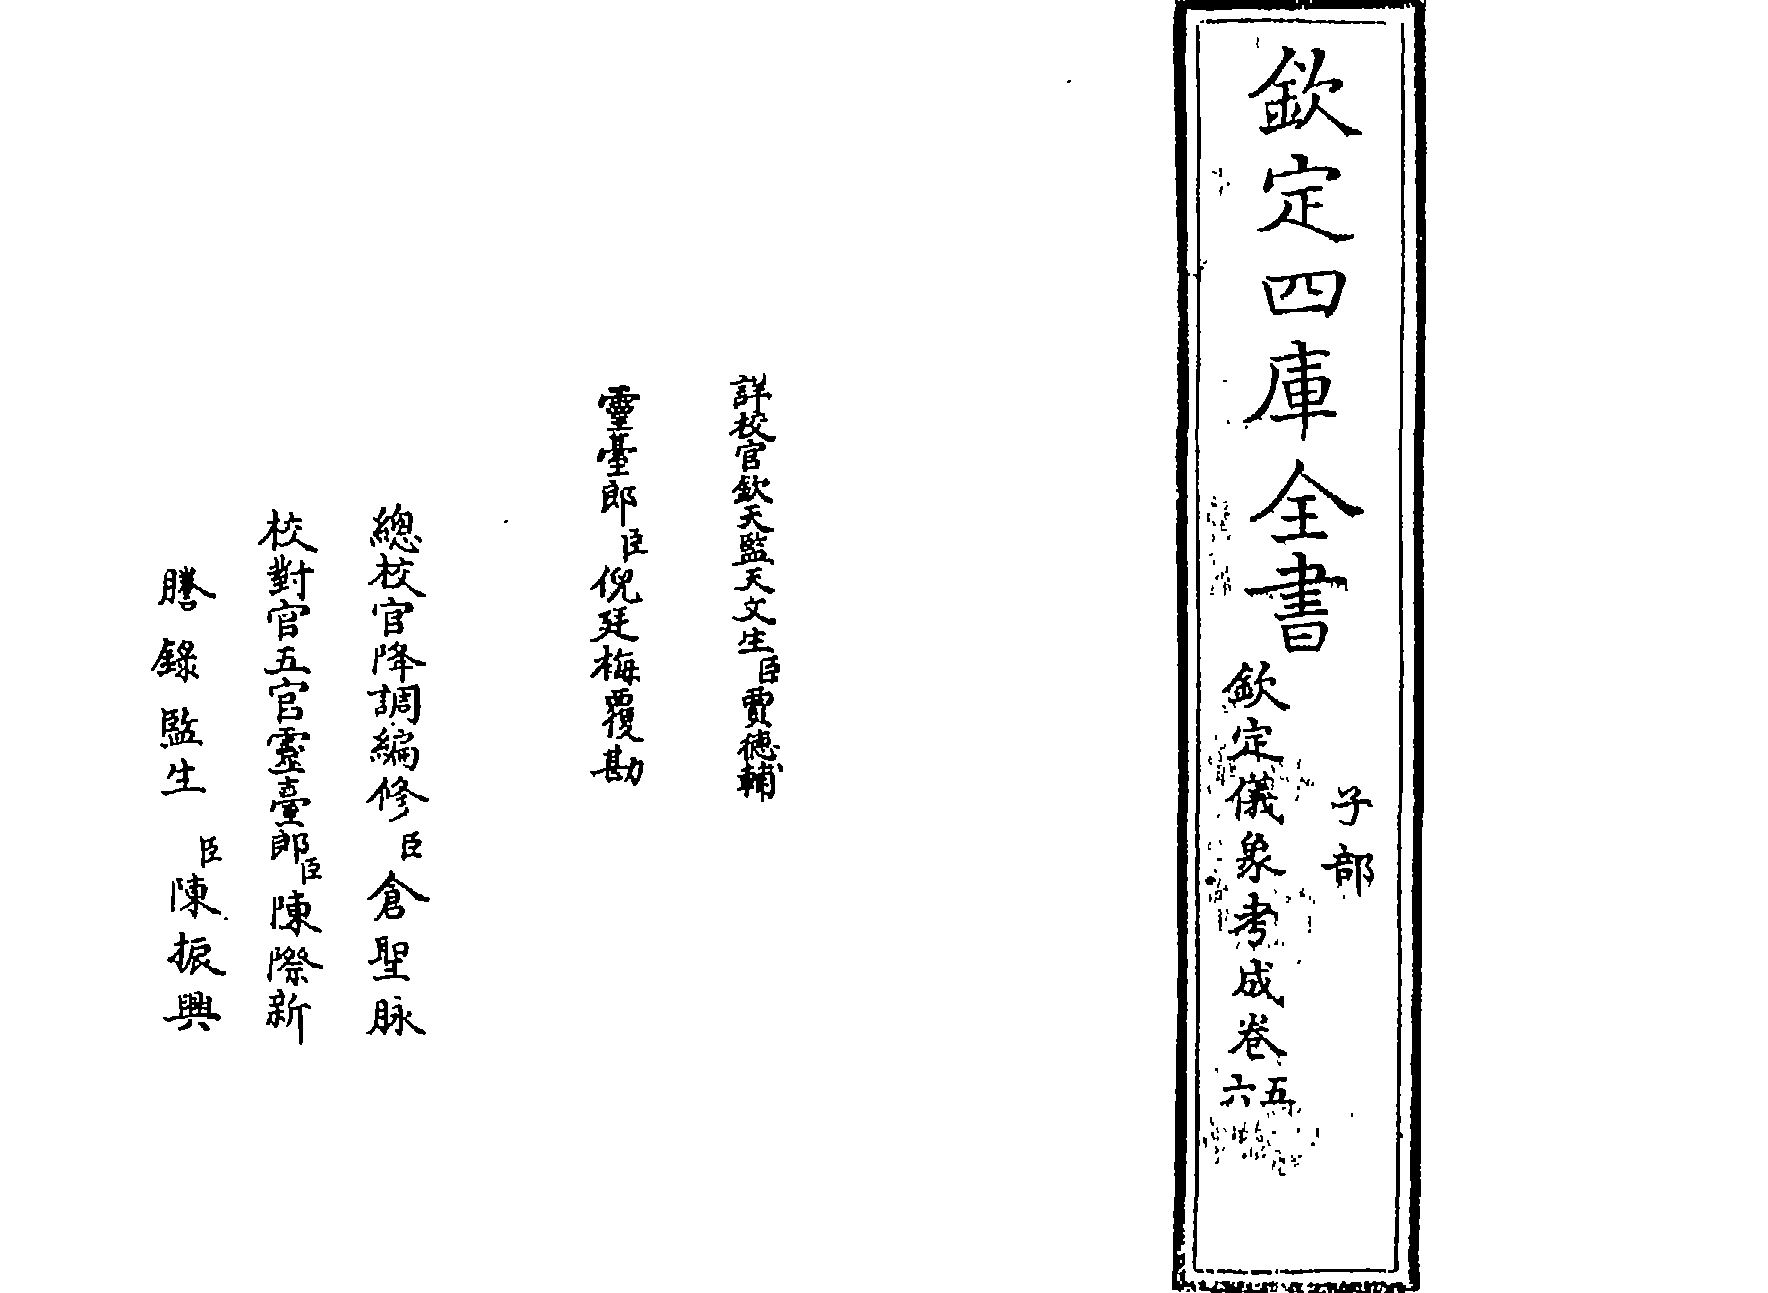
\includegraphics[width=\paperwidth,height=\paperheight,keepaspectratio]{img/0608.png}\clearpage
\begin{正文}
% ---- 册793 葉609 ----
\SetPageNumber{1}
欽定四庫全書\换行
欽定儀象考成卷五\换行
　恒星黄道經緯度表四\换行
　　黄道降婁宫\换行
\char"200B\relax\换行
\char"200B\relax\换行
\char"200B\relax\换行
\char"200B\relax\换行
\char"200B\relax\换行
\char"200B\relax\换行
\char"200B\relax\换行
\char"200B\relax\换行
\char"200B\relax\换行
\char"200B\relax\换行
\char"200B\relax\换行
\char"200B\relax
\par
\end{正文}\clearpage
\嵌图{144.63pt}{201.03pt}{842.50pt}{587.73pt}{img/0612.png}
\begin{正文}
% ---- 册793 葉612 图版 ----
\SetPageNumber{2}
\插图页
\char"200B\relax\换行
\char"200B\relax\换行
\char"200B\relax\换行
\char"200B\relax\换行
\char"200B\relax\换行
\char"200B\relax\换行
\char"200B\relax\换行
\char"200B\relax\换行
\char"200B\relax\换行
\char"200B\relax\换行
\char"200B\relax\换行
\char"200B\relax\换行
\char"200B\relax\换行
\char"200B\relax\换行
\char"200B\relax\换行
\char"200B\relax
\恢复丝栏\par
\end{正文}\clearpage
\嵌图{142.64pt}{201.47pt}{846.47pt}{586.84pt}{img/0613.png}
\begin{正文}
% ---- 册793 葉613 图版 ----
\SetPageNumber{3}
\插图页
\char"200B\relax\换行
\char"200B\relax\换行
\char"200B\relax\换行
\char"200B\relax\换行
\char"200B\relax\换行
\char"200B\relax\换行
\char"200B\relax\换行
\char"200B\relax\换行
\char"200B\relax\换行
\char"200B\relax\换行
\char"200B\relax\换行
\char"200B\relax\换行
\char"200B\relax\换行
\char"200B\relax\换行
\char"200B\relax\换行
\char"200B\relax
\恢复丝栏\par
\end{正文}\clearpage
\嵌图{144.59pt}{201.04pt}{842.59pt}{587.72pt}{img/0616.png}
\begin{正文}
% ---- 册793 葉616 图版 ----
\SetPageNumber{4}
\插图页
\char"200B\relax\换行
\char"200B\relax\换行
\char"200B\relax\换行
\char"200B\relax\换行
\char"200B\relax\换行
\char"200B\relax\换行
\char"200B\relax\换行
\char"200B\relax\换行
\char"200B\relax\换行
\char"200B\relax\换行
\char"200B\relax\换行
\char"200B\relax\换行
\char"200B\relax\换行
\char"200B\relax\换行
\char"200B\relax\换行
\char"200B\relax
\恢复丝栏\par
\end{正文}\clearpage
\嵌图{148.54pt}{201.51pt}{834.68pt}{586.77pt}{img/0617.png}
\begin{正文}
% ---- 册793 葉617 图版 ----
\SetPageNumber{5}
\插图页
\char"200B\relax\换行
\char"200B\relax\换行
\char"200B\relax\换行
\char"200B\relax\换行
\char"200B\relax\换行
\char"200B\relax\换行
\char"200B\relax\换行
\char"200B\relax\换行
\char"200B\relax\换行
\char"200B\relax\换行
\char"200B\relax\换行
\char"200B\relax\换行
\char"200B\relax\换行
\char"200B\relax\换行
\char"200B\relax\换行
\char"200B\relax
\恢复丝栏\par
\end{正文}\clearpage
\嵌图{144.63pt}{201.46pt}{842.50pt}{586.87pt}{img/0620.png}
\begin{正文}
% ---- 册793 葉620 图版 ----
\SetPageNumber{6}
\插图页
\char"200B\relax\换行
\char"200B\relax\换行
\char"200B\relax\换行
\char"200B\relax\换行
\char"200B\relax\换行
\char"200B\relax\换行
\char"200B\relax\换行
\char"200B\relax\换行
\char"200B\relax\换行
\char"200B\relax\换行
\char"200B\relax\换行
\char"200B\relax\换行
\char"200B\relax\换行
\char"200B\relax\换行
\char"200B\relax\换行
\char"200B\relax
\恢复丝栏\par
\end{正文}\clearpage
\嵌图{144.63pt}{201.88pt}{842.50pt}{586.04pt}{img/0621.png}
\begin{正文}
% ---- 册793 葉621 图版 ----
\SetPageNumber{7}
\插图页
\char"200B\relax\换行
\char"200B\relax\换行
\char"200B\relax\换行
\char"200B\relax\换行
\char"200B\relax\换行
\char"200B\relax\换行
\char"200B\relax\换行
\char"200B\relax\换行
\char"200B\relax\换行
\char"200B\relax\换行
\char"200B\relax\换行
\char"200B\relax\换行
\char"200B\relax\换行
\char"200B\relax\换行
\char"200B\relax\换行
\char"200B\relax
\恢复丝栏\par
\end{正文}\clearpage
\嵌图{144.63pt}{202.91pt}{842.50pt}{583.97pt}{img/0624.png}
\begin{正文}
% ---- 册793 葉624 图版 ----
\SetPageNumber{8}
\插图页
\char"200B\relax\换行
\char"200B\relax\换行
\char"200B\relax\换行
\char"200B\relax\换行
\char"200B\relax\换行
\char"200B\relax\换行
\char"200B\relax\换行
\char"200B\relax\换行
\char"200B\relax\换行
\char"200B\relax\换行
\char"200B\relax\换行
\char"200B\relax\换行
\char"200B\relax\换行
\char"200B\relax\换行
\char"200B\relax\换行
\char"200B\relax
\恢复丝栏\par
\end{正文}\clearpage
\嵌图{146.62pt}{203.36pt}{838.53pt}{583.08pt}{img/0625.png}
\begin{正文}
% ---- 册793 葉625 图版 ----
\SetPageNumber{9}
\插图页
\char"200B\relax\换行
\char"200B\relax\换行
\char"200B\relax\换行
\char"200B\relax\换行
\char"200B\relax\换行
\char"200B\relax\换行
\char"200B\relax\换行
\char"200B\relax\换行
\char"200B\relax\换行
\char"200B\relax\换行
\char"200B\relax\换行
\char"200B\relax\换行
\char"200B\relax\换行
\char"200B\relax\换行
\char"200B\relax\换行
\char"200B\relax
\恢复丝栏\par
\end{正文}\clearpage
\嵌图{148.54pt}{201.88pt}{834.68pt}{586.02pt}{img/0628.png}
\begin{正文}
% ---- 册793 葉628 图版 ----
\SetPageNumber{10}
\插图页
\char"200B\relax\换行
\char"200B\relax\换行
\char"200B\relax\换行
\char"200B\relax\换行
\char"200B\relax\换行
\char"200B\relax\换行
\char"200B\relax\换行
\char"200B\relax\换行
\char"200B\relax\换行
\char"200B\relax\换行
\char"200B\relax\换行
\char"200B\relax\换行
\char"200B\relax\换行
\char"200B\relax\换行
\char"200B\relax\换行
\char"200B\relax
\恢复丝栏\par
\end{正文}\clearpage
\嵌图{146.56pt}{200.93pt}{838.64pt}{587.93pt}{img/0629.png}
\begin{正文}
% ---- 册793 葉629 图版 ----
\SetPageNumber{11}
\插图页
\char"200B\relax\换行
\char"200B\relax\换行
\char"200B\relax\换行
\char"200B\relax\换行
\char"200B\relax\换行
\char"200B\relax\换行
\char"200B\relax\换行
\char"200B\relax\换行
\char"200B\relax\换行
\char"200B\relax\换行
\char"200B\relax\换行
\char"200B\relax\换行
\char"200B\relax\换行
\char"200B\relax\换行
\char"200B\relax\换行
\char"200B\relax
\恢复丝栏\par
\end{正文}\clearpage
\嵌图{142.64pt}{201.95pt}{846.47pt}{585.90pt}{img/0632.png}
\begin{正文}
% ---- 册793 葉632 图版 ----
\SetPageNumber{12}
\插图页
\char"200B\relax\换行
\char"200B\relax\换行
\char"200B\relax\换行
\char"200B\relax\换行
\char"200B\relax\换行
\char"200B\relax\换行
\char"200B\relax\换行
\char"200B\relax\换行
\char"200B\relax\换行
\char"200B\relax\换行
\char"200B\relax\换行
\char"200B\relax\换行
\char"200B\relax\换行
\char"200B\relax\换行
\char"200B\relax\换行
\char"200B\relax
\恢复丝栏\par
\end{正文}\clearpage
\嵌图{144.63pt}{200.54pt}{842.50pt}{588.72pt}{img/0633.png}
\begin{正文}
% ---- 册793 葉633 图版 ----
\SetPageNumber{13}
\插图页
\char"200B\relax\换行
\char"200B\relax\换行
\char"200B\relax\换行
\char"200B\relax\换行
\char"200B\relax\换行
\char"200B\relax\换行
\char"200B\relax\换行
\char"200B\relax\换行
\char"200B\relax\换行
\char"200B\relax\换行
\char"200B\relax\换行
\char"200B\relax\换行
\char"200B\relax\换行
\char"200B\relax\换行
\char"200B\relax\换行
\char"200B\relax
\恢复丝栏\par
\end{正文}\clearpage
\嵌图{144.63pt}{200.93pt}{842.50pt}{587.93pt}{img/0636.png}
\begin{正文}
% ---- 册793 葉636 图版 ----
\SetPageNumber{14}
\插图页
\char"200B\relax\换行
\char"200B\relax\换行
\char"200B\relax\换行
\char"200B\relax\换行
\char"200B\relax\换行
\char"200B\relax\换行
\char"200B\relax\换行
\char"200B\relax\换行
\char"200B\relax\换行
\char"200B\relax\换行
\char"200B\relax\换行
\char"200B\relax\换行
\char"200B\relax\换行
\char"200B\relax\换行
\char"200B\relax\换行
\char"200B\relax
\恢复丝栏\par
\end{正文}\clearpage
\嵌图{148.61pt}{199.50pt}{834.55pt}{590.78pt}{img/0637.png}
\begin{正文}
% ---- 册793 葉637 图版 ----
\SetPageNumber{15}
\插图页
\char"200B\relax\换行
\char"200B\relax\换行
\char"200B\relax\换行
\char"200B\relax\换行
\char"200B\relax\换行
\char"200B\relax\换行
\char"200B\relax\换行
\char"200B\relax\换行
\char"200B\relax\换行
\char"200B\relax\换行
\char"200B\relax\换行
\char"200B\relax\换行
\char"200B\relax\换行
\char"200B\relax\换行
\char"200B\relax\换行
\char"200B\relax
\恢复丝栏\par
\end{正文}\clearpage
\嵌图{144.63pt}{201.95pt}{842.50pt}{585.90pt}{img/0640.png}
\begin{正文}
% ---- 册793 葉640 图版 ----
\SetPageNumber{16}
\插图页
\char"200B\relax\换行
\char"200B\relax\换行
\char"200B\relax\换行
\char"200B\relax\换行
\char"200B\relax\换行
\char"200B\relax\换行
\char"200B\relax\换行
\char"200B\relax\换行
\char"200B\relax\换行
\char"200B\relax\换行
\char"200B\relax\换行
\char"200B\relax\换行
\char"200B\relax\换行
\char"200B\relax\换行
\char"200B\relax\换行
\char"200B\relax
\恢复丝栏\par
\end{正文}\clearpage
\嵌图{144.63pt}{201.02pt}{842.50pt}{587.76pt}{img/0641.png}
\begin{正文}
% ---- 册793 葉641 图版 ----
\SetPageNumber{17}
\插图页
\char"200B\relax\换行
\char"200B\relax\换行
\char"200B\relax\换行
\char"200B\relax\换行
\char"200B\relax\换行
\char"200B\relax\换行
\char"200B\relax\换行
\char"200B\relax\换行
\char"200B\relax\换行
\char"200B\relax\换行
\char"200B\relax\换行
\char"200B\relax\换行
\char"200B\relax\换行
\char"200B\relax\换行
\char"200B\relax\换行
\char"200B\relax
\恢复丝栏\par
\end{正文}\clearpage
\嵌图{146.67pt}{200.52pt}{838.42pt}{588.75pt}{img/0644.png}
\begin{正文}
% ---- 册793 葉644 图版 ----
\SetPageNumber{18}
\插图页
\char"200B\relax\换行
\char"200B\relax\换行
\char"200B\relax\换行
\char"200B\relax\换行
\char"200B\relax\换行
\char"200B\relax\换行
\char"200B\relax\换行
\char"200B\relax\换行
\char"200B\relax\换行
\char"200B\relax\换行
\char"200B\relax\换行
\char"200B\relax\换行
\char"200B\relax\换行
\char"200B\relax\换行
\char"200B\relax\换行
\char"200B\relax
\恢复丝栏\par
\end{正文}\clearpage
\嵌图{150.67pt}{200.99pt}{830.43pt}{587.80pt}{img/0645.png}
\begin{正文}
% ---- 册793 葉645 图版 ----
\SetPageNumber{19}
\插图页
\char"200B\relax\换行
\char"200B\relax\换行
\char"200B\relax\换行
\char"200B\relax\换行
\char"200B\relax\换行
\char"200B\relax\换行
\char"200B\relax\换行
\char"200B\relax\换行
\char"200B\relax\换行
\char"200B\relax\换行
\char"200B\relax\换行
\char"200B\relax\换行
\char"200B\relax\换行
\char"200B\relax\换行
\char"200B\relax\换行
\char"200B\relax
\恢复丝栏\par
\end{正文}\clearpage
\嵌图{140.63pt}{199.98pt}{850.50pt}{589.83pt}{img/0648.png}
\begin{正文}
% ---- 册793 葉648 图版 ----
\SetPageNumber{20}
\插图页
\char"200B\relax\换行
\char"200B\relax\换行
\char"200B\relax\换行
\char"200B\relax\换行
\char"200B\relax\换行
\char"200B\relax\换行
\char"200B\relax\换行
\char"200B\relax\换行
\char"200B\relax\换行
\char"200B\relax\换行
\char"200B\relax\换行
\char"200B\relax\换行
\char"200B\relax\换行
\char"200B\relax\换行
\char"200B\relax\换行
\char"200B\relax
\恢复丝栏\par
\end{正文}\clearpage
\嵌图{146.56pt}{200.49pt}{838.64pt}{588.82pt}{img/0649.png}
\begin{正文}
% ---- 册793 葉649 图版 ----
\SetPageNumber{21}
\插图页
\char"200B\relax\换行
\char"200B\relax\换行
\char"200B\relax\换行
\char"200B\relax\换行
\char"200B\relax\换行
\char"200B\relax\换行
\char"200B\relax\换行
\char"200B\relax\换行
\char"200B\relax\换行
\char"200B\relax\换行
\char"200B\relax\换行
\char"200B\relax\换行
\char"200B\relax\换行
\char"200B\relax\换行
\char"200B\relax\换行
\char"200B\relax
\恢复丝栏\par
\end{正文}\clearpage
\嵌图{126.91pt}{215.07pt}{762.93pt}{577.76pt}{img/0652.png}
\begin{正文}
% ---- 册793 葉652 ----
\SetPageNumber{22}
\插图页
\char"200B\relax\换行
\char"200B\relax\换行
\char"200B\relax\换行
\char"200B\relax\换行
\char"200B\relax\换行
\char"200B\relax\换行
\char"200B\relax\换行
\char"200B\relax\换行
\恢复丝栏
\char"200B\relax\换行
\char"200B\relax\换行
\char"200B\relax\换行
\char"200B\relax\换行
\char"200B\relax\换行
\char"200B\relax\换行
欽定儀象考成卷五\换行
\char"200B\relax
\par

% ======== 卷六（8行21字）========
\par\end{正文}\clearpage
\chapter*{欽定儀象考成卷六}
\begin{正文}
% ---- 册793 葉653 ----
\SetPageNumber{1}
欽定四庫全書\换行
欽定儀象考成卷六\换行
　恒星黄道經緯度表五\换行
　　黄道大梁宫\双列{\右小列{赤道度附}\左小列{}}\换行
\char"200B\relax\换行
\char"200B\relax\换行
\char"200B\relax\换行
\char"200B\relax\换行
\char"200B\relax\换行
\char"200B\relax\换行
\char"200B\relax\换行
\char"200B\relax\换行
\char"200B\relax\换行
\char"200B\relax\换行
\char"200B\relax\换行
\char"200B\relax
\par
\end{正文}\clearpage
\嵌图{142.68pt}{198.67pt}{846.40pt}{592.45pt}{img/0656.png}
\begin{正文}
% ---- 册793 葉656 图版 ----
\SetPageNumber{2}
\插图页
\char"200B\relax\换行
\char"200B\relax\换行
\char"200B\relax\换行
\char"200B\relax\换行
\char"200B\relax\换行
\char"200B\relax\换行
\char"200B\relax\换行
\char"200B\relax\换行
\char"200B\relax\换行
\char"200B\relax\换行
\char"200B\relax\换行
\char"200B\relax\换行
\char"200B\relax\换行
\char"200B\relax\换行
\char"200B\relax\换行
\char"200B\relax
\恢复丝栏\par
\end{正文}\clearpage
\嵌图{146.67pt}{203.90pt}{838.42pt}{582.00pt}{img/0657.png}
\begin{正文}
% ---- 册793 葉657 图版 ----
\SetPageNumber{3}
\插图页
\char"200B\relax\换行
\char"200B\relax\换行
\char"200B\relax\换行
\char"200B\relax\换行
\char"200B\relax\换行
\char"200B\relax\换行
\char"200B\relax\换行
\char"200B\relax\换行
\char"200B\relax\换行
\char"200B\relax\换行
\char"200B\relax\换行
\char"200B\relax\换行
\char"200B\relax\换行
\char"200B\relax\换行
\char"200B\relax\换行
\char"200B\relax
\恢复丝栏\par
\end{正文}\clearpage
\嵌图{148.61pt}{201.92pt}{834.55pt}{585.94pt}{img/0660.png}
\begin{正文}
% ---- 册793 葉660 图版 ----
\SetPageNumber{4}
\插图页
\char"200B\relax\换行
\char"200B\relax\换行
\char"200B\relax\换行
\char"200B\relax\换行
\char"200B\relax\换行
\char"200B\relax\换行
\char"200B\relax\换行
\char"200B\relax\换行
\char"200B\relax\换行
\char"200B\relax\换行
\char"200B\relax\换行
\char"200B\relax\换行
\char"200B\relax\换行
\char"200B\relax\换行
\char"200B\relax\换行
\char"200B\relax
\恢复丝栏\par
\end{正文}\clearpage
\嵌图{146.62pt}{201.41pt}{838.53pt}{586.96pt}{img/0661.png}
\begin{正文}
% ---- 册793 葉661 图版 ----
\SetPageNumber{5}
\插图页
\char"200B\relax\换行
\char"200B\relax\换行
\char"200B\relax\换行
\char"200B\relax\换行
\char"200B\relax\换行
\char"200B\relax\换行
\char"200B\relax\换行
\char"200B\relax\换行
\char"200B\relax\换行
\char"200B\relax\换行
\char"200B\relax\换行
\char"200B\relax\换行
\char"200B\relax\换行
\char"200B\relax\换行
\char"200B\relax\换行
\char"200B\relax
\恢复丝栏\par
\end{正文}\clearpage
\嵌图{146.67pt}{201.55pt}{838.42pt}{586.69pt}{img/0664.png}
\begin{正文}
% ---- 册793 葉664 图版 ----
\SetPageNumber{6}
\插图页
\char"200B\relax\换行
\char"200B\relax\换行
\char"200B\relax\换行
\char"200B\relax\换行
\char"200B\relax\换行
\char"200B\relax\换行
\char"200B\relax\换行
\char"200B\relax\换行
\char"200B\relax\换行
\char"200B\relax\换行
\char"200B\relax\换行
\char"200B\relax\换行
\char"200B\relax\换行
\char"200B\relax\换行
\char"200B\relax\换行
\char"200B\relax
\恢复丝栏\par
\end{正文}\clearpage
\嵌图{144.68pt}{200.53pt}{842.41pt}{588.73pt}{img/0665.png}
\begin{正文}
% ---- 册793 葉665 图版 ----
\SetPageNumber{7}
\插图页
\char"200B\relax\换行
\char"200B\relax\换行
\char"200B\relax\换行
\char"200B\relax\换行
\char"200B\relax\换行
\char"200B\relax\换行
\char"200B\relax\换行
\char"200B\relax\换行
\char"200B\relax\换行
\char"200B\relax\换行
\char"200B\relax\换行
\char"200B\relax\换行
\char"200B\relax\换行
\char"200B\relax\换行
\char"200B\relax\换行
\char"200B\relax
\恢复丝栏\par
\end{正文}\clearpage
\嵌图{146.67pt}{200.50pt}{838.42pt}{588.79pt}{img/0668.png}
\begin{正文}
% ---- 册793 葉668 图版 ----
\SetPageNumber{8}
\插图页
\char"200B\relax\换行
\char"200B\relax\换行
\char"200B\relax\换行
\char"200B\relax\换行
\char"200B\relax\换行
\char"200B\relax\换行
\char"200B\relax\换行
\char"200B\relax\换行
\char"200B\relax\换行
\char"200B\relax\换行
\char"200B\relax\换行
\char"200B\relax\换行
\char"200B\relax\换行
\char"200B\relax\换行
\char"200B\relax\换行
\char"200B\relax
\恢复丝栏\par
\end{正文}\clearpage
\嵌图{148.67pt}{199.52pt}{834.42pt}{590.75pt}{img/0669.png}
\begin{正文}
% ---- 册793 葉669 图版 ----
\SetPageNumber{9}
\插图页
\char"200B\relax\换行
\char"200B\relax\换行
\char"200B\relax\换行
\char"200B\relax\换行
\char"200B\relax\换行
\char"200B\relax\换行
\char"200B\relax\换行
\char"200B\relax\换行
\char"200B\relax\换行
\char"200B\relax\换行
\char"200B\relax\换行
\char"200B\relax\换行
\char"200B\relax\换行
\char"200B\relax\换行
\char"200B\relax\换行
\char"200B\relax
\恢复丝栏\par
\end{正文}\clearpage
\嵌图{144.63pt}{201.94pt}{842.50pt}{585.91pt}{img/0672.png}
\begin{正文}
% ---- 册793 葉672 图版 ----
\SetPageNumber{10}
\插图页
\char"200B\relax\换行
\char"200B\relax\换行
\char"200B\relax\换行
\char"200B\relax\换行
\char"200B\relax\换行
\char"200B\relax\换行
\char"200B\relax\换行
\char"200B\relax\换行
\char"200B\relax\换行
\char"200B\relax\换行
\char"200B\relax\换行
\char"200B\relax\换行
\char"200B\relax\换行
\char"200B\relax\换行
\char"200B\relax\换行
\char"200B\relax
\恢复丝栏\par
\end{正文}\clearpage
\嵌图{144.63pt}{202.90pt}{842.50pt}{583.99pt}{img/0673.png}
\begin{正文}
% ---- 册793 葉673 图版 ----
\SetPageNumber{11}
\插图页
\char"200B\relax\换行
\char"200B\relax\换行
\char"200B\relax\换行
\char"200B\relax\换行
\char"200B\relax\换行
\char"200B\relax\换行
\char"200B\relax\换行
\char"200B\relax\换行
\char"200B\relax\换行
\char"200B\relax\换行
\char"200B\relax\换行
\char"200B\relax\换行
\char"200B\relax\换行
\char"200B\relax\换行
\char"200B\relax\换行
\char"200B\relax
\恢复丝栏\par
\end{正文}\clearpage
\嵌图{148.73pt}{201.95pt}{834.29pt}{585.88pt}{img/0676.png}
\begin{正文}
% ---- 册793 葉676 图版 ----
\SetPageNumber{12}
\插图页
\char"200B\relax\换行
\char"200B\relax\换行
\char"200B\relax\换行
\char"200B\relax\换行
\char"200B\relax\换行
\char"200B\relax\换行
\char"200B\relax\换行
\char"200B\relax\换行
\char"200B\relax\换行
\char"200B\relax\换行
\char"200B\relax\换行
\char"200B\relax\换行
\char"200B\relax\换行
\char"200B\relax\换行
\char"200B\relax\换行
\char"200B\relax
\恢复丝栏\par
\end{正文}\clearpage
\嵌图{146.73pt}{198.17pt}{838.30pt}{593.45pt}{img/0677.png}
\begin{正文}
% ---- 册793 葉677 图版 ----
\SetPageNumber{13}
\插图页
\char"200B\relax\换行
\char"200B\relax\换行
\char"200B\relax\换行
\char"200B\relax\换行
\char"200B\relax\换行
\char"200B\relax\换行
\char"200B\relax\换行
\char"200B\relax\换行
\char"200B\relax\换行
\char"200B\relax\换行
\char"200B\relax\换行
\char"200B\relax\换行
\char"200B\relax\换行
\char"200B\relax\换行
\char"200B\relax\换行
\char"200B\relax
\恢复丝栏\par
\end{正文}\clearpage
\嵌图{146.56pt}{202.90pt}{838.64pt}{583.99pt}{img/0680.png}
\begin{正文}
% ---- 册793 葉680 图版 ----
\SetPageNumber{14}
\插图页
\char"200B\relax\换行
\char"200B\relax\换行
\char"200B\relax\换行
\char"200B\relax\换行
\char"200B\relax\换行
\char"200B\relax\换行
\char"200B\relax\换行
\char"200B\relax\换行
\char"200B\relax\换行
\char"200B\relax\换行
\char"200B\relax\换行
\char"200B\relax\换行
\char"200B\relax\换行
\char"200B\relax\换行
\char"200B\relax\换行
\char"200B\relax
\恢复丝栏\par
\end{正文}\clearpage
\嵌图{148.54pt}{205.26pt}{834.68pt}{579.28pt}{img/0681.png}
\begin{正文}
% ---- 册793 葉681 图版 ----
\SetPageNumber{15}
\插图页
\char"200B\relax\换行
\char"200B\relax\换行
\char"200B\relax\换行
\char"200B\relax\换行
\char"200B\relax\换行
\char"200B\relax\换行
\char"200B\relax\换行
\char"200B\relax\换行
\char"200B\relax\换行
\char"200B\relax\换行
\char"200B\relax\换行
\char"200B\relax\换行
\char"200B\relax\换行
\char"200B\relax\换行
\char"200B\relax\换行
\char"200B\relax
\恢复丝栏\par
\end{正文}\clearpage
\嵌图{146.56pt}{203.84pt}{838.64pt}{582.11pt}{img/0684.png}
\begin{正文}
% ---- 册793 葉684 图版 ----
\SetPageNumber{16}
\插图页
\char"200B\relax\换行
\char"200B\relax\换行
\char"200B\relax\换行
\char"200B\relax\换行
\char"200B\relax\换行
\char"200B\relax\换行
\char"200B\relax\换行
\char"200B\relax\换行
\char"200B\relax\换行
\char"200B\relax\换行
\char"200B\relax\换行
\char"200B\relax\换行
\char"200B\relax\换行
\char"200B\relax\换行
\char"200B\relax\换行
\char"200B\relax
\恢复丝栏\par
\end{正文}\clearpage
\嵌图{146.56pt}{200.49pt}{838.64pt}{588.80pt}{img/0685.png}
\begin{正文}
% ---- 册793 葉685 图版 ----
\SetPageNumber{17}
\插图页
\char"200B\relax\换行
\char"200B\relax\换行
\char"200B\relax\换行
\char"200B\relax\换行
\char"200B\relax\换行
\char"200B\relax\换行
\char"200B\relax\换行
\char"200B\relax\换行
\char"200B\relax\换行
\char"200B\relax\换行
\char"200B\relax\换行
\char"200B\relax\换行
\char"200B\relax\换行
\char"200B\relax\换行
\char"200B\relax\换行
\char"200B\relax
\恢复丝栏\par
\end{正文}\clearpage
\嵌图{140.68pt}{203.93pt}{850.39pt}{581.92pt}{img/0688.png}
\begin{正文}
% ---- 册793 葉688 图版 ----
\SetPageNumber{18}
\插图页
\char"200B\relax\换行
\char"200B\relax\换行
\char"200B\relax\换行
\char"200B\relax\换行
\char"200B\relax\换行
\char"200B\relax\换行
\char"200B\relax\换行
\char"200B\relax\换行
\char"200B\relax\换行
\char"200B\relax\换行
\char"200B\relax\换行
\char"200B\relax\换行
\char"200B\relax\换行
\char"200B\relax\换行
\char"200B\relax\换行
\char"200B\relax
\恢复丝栏\par
\end{正文}\clearpage
\嵌图{150.67pt}{200.58pt}{830.43pt}{588.62pt}{img/0689.png}
\begin{正文}
% ---- 册793 葉689 图版 ----
\SetPageNumber{19}
\插图页
\char"200B\relax\换行
\char"200B\relax\换行
\char"200B\relax\换行
\char"200B\relax\换行
\char"200B\relax\换行
\char"200B\relax\换行
\char"200B\relax\换行
\char"200B\relax\换行
\char"200B\relax\换行
\char"200B\relax\换行
\char"200B\relax\换行
\char"200B\relax\换行
\char"200B\relax\换行
\char"200B\relax\换行
\char"200B\relax\换行
\char"200B\relax
\恢复丝栏\par
\end{正文}\clearpage
\嵌图{148.61pt}{201.93pt}{834.55pt}{585.93pt}{img/0692.png}
\begin{正文}
% ---- 册793 葉692 图版 ----
\SetPageNumber{20}
\插图页
\char"200B\relax\换行
\char"200B\relax\换行
\char"200B\relax\换行
\char"200B\relax\换行
\char"200B\relax\换行
\char"200B\relax\换行
\char"200B\relax\换行
\char"200B\relax\换行
\char"200B\relax\换行
\char"200B\relax\换行
\char"200B\relax\换行
\char"200B\relax\换行
\char"200B\relax\换行
\char"200B\relax\换行
\char"200B\relax\换行
\char"200B\relax
\恢复丝栏\par
\end{正文}\clearpage
\嵌图{146.62pt}{204.25pt}{838.53pt}{581.28pt}{img/0693.png}
\begin{正文}
% ---- 册793 葉693 图版 ----
\SetPageNumber{21}
\插图页
\char"200B\relax\换行
\char"200B\relax\换行
\char"200B\relax\换行
\char"200B\relax\换行
\char"200B\relax\换行
\char"200B\relax\换行
\char"200B\relax\换行
\char"200B\relax\换行
\char"200B\relax\换行
\char"200B\relax\换行
\char"200B\relax\换行
\char"200B\relax\换行
\char"200B\relax\换行
\char"200B\relax\换行
\char"200B\relax\换行
\char"200B\relax
\恢复丝栏\par
\end{正文}\clearpage
\嵌图{144.72pt}{203.93pt}{842.31pt}{581.92pt}{img/0696.png}
\begin{正文}
% ---- 册793 葉696 图版 ----
\SetPageNumber{22}
\插图页
\char"200B\relax\换行
\char"200B\relax\换行
\char"200B\relax\换行
\char"200B\relax\换行
\char"200B\relax\换行
\char"200B\relax\换行
\char"200B\relax\换行
\char"200B\relax\换行
\char"200B\relax\换行
\char"200B\relax\换行
\char"200B\relax\换行
\char"200B\relax\换行
\char"200B\relax\换行
\char"200B\relax\换行
\char"200B\relax\换行
\char"200B\relax
\恢复丝栏\par
\end{正文}\clearpage
\嵌图{164.65pt}{222.62pt}{725.19pt}{570.21pt}{img/0697.png}
\begin{正文}
% ---- 册793 葉697 ----
\SetPageNumber{23}
\插图页
\char"200B\relax\换行
\char"200B\relax\换行
\char"200B\relax\换行
\char"200B\relax\换行
\char"200B\relax\换行
\char"200B\relax\换行
\char"200B\relax\换行
\char"200B\relax\换行
\恢复丝栏
\char"200B\relax\换行
\char"200B\relax\换行
\char"200B\relax\换行
\char"200B\relax\换行
\char"200B\relax\换行
\char"200B\relax\换行
\char"200B\relax\换行
欽定儀象考成卷六
\par

\par\end{正文}\clearpage

  \input{parts/part07}
  \thispagestyle{empty}\noindent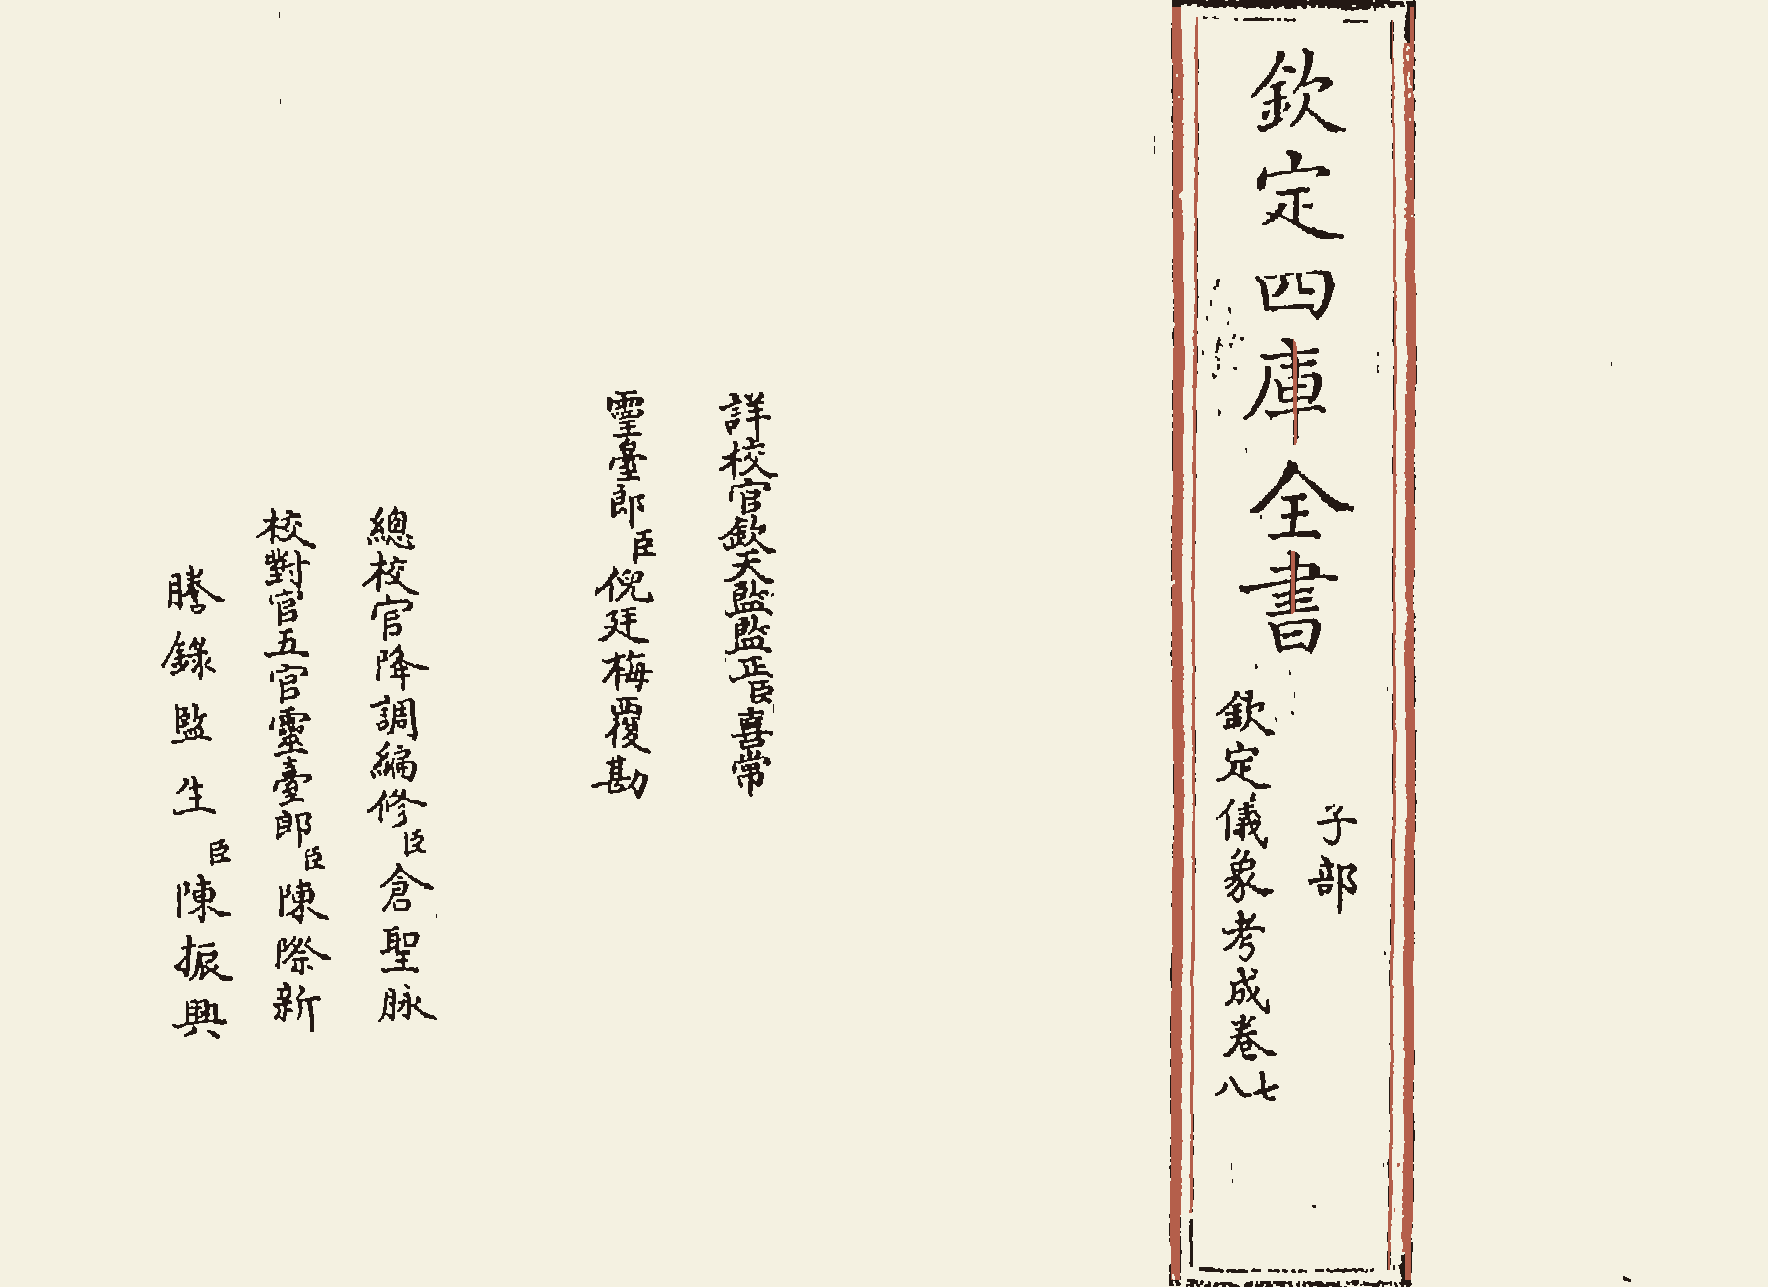
\includegraphics[width=\paperwidth,height=\paperheight,keepaspectratio]{img/0700.png}\clearpage
\begin{正文}
% ---- 册793 葉701 ----
\SetPageNumber{1}
欽定四庫全書\换行
欽定儀象考成卷七\换行
　恒星黄道經緯度表六\换行
　　黄道實沈宫\双列{\右小列{赤道度附}\左小列{}}\换行
\char"200B\relax\换行
\char"200B\relax\换行
\char"200B\relax\换行
\char"200B\relax\换行
\char"200B\relax\换行
\char"200B\relax\换行
\char"200B\relax\换行
\char"200B\relax\换行
\char"200B\relax\换行
\char"200B\relax\换行
\char"200B\relax\换行
\char"200B\relax
\par
\end{正文}\clearpage
\嵌图{146.56pt}{202.48pt}{838.64pt}{584.83pt}{img/0704.png}
\begin{正文}
% ---- 册793 葉704 图版 ----
\SetPageNumber{2}
\插图页
\char"200B\relax\换行
\char"200B\relax\换行
\char"200B\relax\换行
\char"200B\relax\换行
\char"200B\relax\换行
\char"200B\relax\换行
\char"200B\relax\换行
\char"200B\relax\换行
\char"200B\relax\换行
\char"200B\relax\换行
\char"200B\relax\换行
\char"200B\relax\换行
\char"200B\relax\换行
\char"200B\relax\换行
\char"200B\relax\换行
\char"200B\relax
\恢复丝栏\par
\end{正文}\clearpage
\嵌图{148.54pt}{201.50pt}{834.68pt}{586.80pt}{img/0705.png}
\begin{正文}
% ---- 册793 葉705 图版 ----
\SetPageNumber{3}
\插图页
\char"200B\relax\换行
\char"200B\relax\换行
\char"200B\relax\换行
\char"200B\relax\换行
\char"200B\relax\换行
\char"200B\relax\换行
\char"200B\relax\换行
\char"200B\relax\换行
\char"200B\relax\换行
\char"200B\relax\换行
\char"200B\relax\换行
\char"200B\relax\换行
\char"200B\relax\换行
\char"200B\relax\换行
\char"200B\relax\换行
\char"200B\relax
\恢复丝栏\par
\end{正文}\clearpage
\嵌图{146.62pt}{203.90pt}{838.53pt}{582.00pt}{img/0708.png}
\begin{正文}
% ---- 册793 葉708 图版 ----
\SetPageNumber{4}
\插图页
\char"200B\relax\换行
\char"200B\relax\换行
\char"200B\relax\换行
\char"200B\relax\换行
\char"200B\relax\换行
\char"200B\relax\换行
\char"200B\relax\换行
\char"200B\relax\换行
\char"200B\relax\换行
\char"200B\relax\换行
\char"200B\relax\换行
\char"200B\relax\换行
\char"200B\relax\换行
\char"200B\relax\换行
\char"200B\relax\换行
\char"200B\relax
\恢复丝栏\par
\end{正文}\clearpage
\嵌图{144.63pt}{200.99pt}{842.50pt}{587.82pt}{img/0709.png}
\begin{正文}
% ---- 册793 葉709 图版 ----
\SetPageNumber{5}
\插图页
\char"200B\relax\换行
\char"200B\relax\换行
\char"200B\relax\换行
\char"200B\relax\换行
\char"200B\relax\换行
\char"200B\relax\换行
\char"200B\relax\换行
\char"200B\relax\换行
\char"200B\relax\换行
\char"200B\relax\换行
\char"200B\relax\换行
\char"200B\relax\换行
\char"200B\relax\换行
\char"200B\relax\换行
\char"200B\relax\换行
\char"200B\relax
\恢复丝栏\par
\end{正文}\clearpage
\嵌图{140.66pt}{204.85pt}{850.45pt}{580.10pt}{img/0712.png}
\begin{正文}
% ---- 册793 葉712 图版 ----
\SetPageNumber{6}
\插图页
\char"200B\relax\换行
\char"200B\relax\换行
\char"200B\relax\换行
\char"200B\relax\换行
\char"200B\relax\换行
\char"200B\relax\换行
\char"200B\relax\换行
\char"200B\relax\换行
\char"200B\relax\换行
\char"200B\relax\换行
\char"200B\relax\换行
\char"200B\relax\换行
\char"200B\relax\换行
\char"200B\relax\换行
\char"200B\relax\换行
\char"200B\relax
\恢复丝栏\par
\end{正文}\clearpage
\嵌图{142.64pt}{204.81pt}{846.47pt}{580.16pt}{img/0713.png}
\begin{正文}
% ---- 册793 葉713 图版 ----
\SetPageNumber{7}
\插图页
\char"200B\relax\换行
\char"200B\relax\换行
\char"200B\relax\换行
\char"200B\relax\换行
\char"200B\relax\换行
\char"200B\relax\换行
\char"200B\relax\换行
\char"200B\relax\换行
\char"200B\relax\换行
\char"200B\relax\换行
\char"200B\relax\换行
\char"200B\relax\换行
\char"200B\relax\换行
\char"200B\relax\换行
\char"200B\relax\换行
\char"200B\relax
\恢复丝栏\par
\end{正文}\clearpage
\嵌图{148.54pt}{198.60pt}{834.68pt}{592.58pt}{img/0716.png}
\begin{正文}
% ---- 册793 葉716 图版 ----
\SetPageNumber{8}
\插图页
\char"200B\relax\换行
\char"200B\relax\换行
\char"200B\relax\换行
\char"200B\relax\换行
\char"200B\relax\换行
\char"200B\relax\换行
\char"200B\relax\换行
\char"200B\relax\换行
\char"200B\relax\换行
\char"200B\relax\换行
\char"200B\relax\换行
\char"200B\relax\换行
\char"200B\relax\换行
\char"200B\relax\换行
\char"200B\relax\换行
\char"200B\relax
\恢复丝栏\par
\end{正文}\clearpage
\嵌图{150.52pt}{200.46pt}{830.72pt}{588.87pt}{img/0717.png}
\begin{正文}
% ---- 册793 葉717 图版 ----
\SetPageNumber{9}
\插图页
\char"200B\relax\换行
\char"200B\relax\换行
\char"200B\relax\换行
\char"200B\relax\换行
\char"200B\relax\换行
\char"200B\relax\换行
\char"200B\relax\换行
\char"200B\relax\换行
\char"200B\relax\换行
\char"200B\relax\换行
\char"200B\relax\换行
\char"200B\relax\换行
\char"200B\relax\换行
\char"200B\relax\换行
\char"200B\relax\换行
\char"200B\relax
\恢复丝栏\par
\end{正文}\clearpage
\嵌图{142.64pt}{200.54pt}{846.47pt}{588.72pt}{img/0720.png}
\begin{正文}
% ---- 册793 葉720 图版 ----
\SetPageNumber{10}
\插图页
\char"200B\relax\换行
\char"200B\relax\换行
\char"200B\relax\换行
\char"200B\relax\换行
\char"200B\relax\换行
\char"200B\relax\换行
\char"200B\relax\换行
\char"200B\relax\换行
\char"200B\relax\换行
\char"200B\relax\换行
\char"200B\relax\换行
\char"200B\relax\换行
\char"200B\relax\换行
\char"200B\relax\换行
\char"200B\relax\换行
\char"200B\relax
\恢复丝栏\par
\end{正文}\clearpage
\嵌图{150.59pt}{203.37pt}{830.58pt}{583.06pt}{img/0721.png}
\begin{正文}
% ---- 册793 葉721 图版 ----
\SetPageNumber{11}
\插图页
\char"200B\relax\换行
\char"200B\relax\换行
\char"200B\relax\换行
\char"200B\relax\换行
\char"200B\relax\换行
\char"200B\relax\换行
\char"200B\relax\换行
\char"200B\relax\换行
\char"200B\relax\换行
\char"200B\relax\换行
\char"200B\relax\换行
\char"200B\relax\换行
\char"200B\relax\换行
\char"200B\relax\换行
\char"200B\relax\换行
\char"200B\relax
\恢复丝栏\par
\end{正文}\clearpage
\嵌图{365.19pt}{199.32pt}{401.38pt}{591.16pt}{img/0724.png}
\begin{正文}
% ---- 册793 葉724 图版 ----
\SetPageNumber{12}
\插图页
\char"200B\relax\换行
\char"200B\relax\换行
\char"200B\relax\换行
\char"200B\relax\换行
\char"200B\relax\换行
\char"200B\relax\换行
\char"200B\relax\换行
\char"200B\relax\换行
\char"200B\relax\换行
\char"200B\relax\换行
\char"200B\relax\换行
\char"200B\relax\换行
\char"200B\relax\换行
\char"200B\relax\换行
\char"200B\relax\换行
\char"200B\relax
\恢复丝栏\par
\end{正文}\clearpage
\嵌图{363.20pt}{202.59pt}{405.35pt}{584.61pt}{img/0725.png}
\begin{正文}
% ---- 册793 葉725 图版 ----
\SetPageNumber{13}
\插图页
\char"200B\relax\换行
\char"200B\relax\换行
\char"200B\relax\换行
\char"200B\relax\换行
\char"200B\relax\换行
\char"200B\relax\换行
\char"200B\relax\换行
\char"200B\relax\换行
\char"200B\relax\换行
\char"200B\relax\换行
\char"200B\relax\换行
\char"200B\relax\换行
\char"200B\relax\换行
\char"200B\relax\换行
\char"200B\relax\换行
\char"200B\relax
\恢复丝栏\par
\end{正文}\clearpage
\嵌图{144.68pt}{200.99pt}{842.41pt}{587.82pt}{img/0728.png}
\begin{正文}
% ---- 册793 葉728 图版 ----
\SetPageNumber{14}
\插图页
\char"200B\relax\换行
\char"200B\relax\换行
\char"200B\relax\换行
\char"200B\relax\换行
\char"200B\relax\换行
\char"200B\relax\换行
\char"200B\relax\换行
\char"200B\relax\换行
\char"200B\relax\换行
\char"200B\relax\换行
\char"200B\relax\换行
\char"200B\relax\换行
\char"200B\relax\换行
\char"200B\relax\换行
\char"200B\relax\换行
\char"200B\relax
\恢复丝栏\par
\end{正文}\clearpage
\嵌图{148.67pt}{203.37pt}{834.42pt}{583.06pt}{img/0729.png}
\begin{正文}
% ---- 册793 葉729 图版 ----
\SetPageNumber{15}
\插图页
\char"200B\relax\换行
\char"200B\relax\换行
\char"200B\relax\换行
\char"200B\relax\换行
\char"200B\relax\换行
\char"200B\relax\换行
\char"200B\relax\换行
\char"200B\relax\换行
\char"200B\relax\换行
\char"200B\relax\换行
\char"200B\relax\换行
\char"200B\relax\换行
\char"200B\relax\换行
\char"200B\relax\换行
\char"200B\relax\换行
\char"200B\relax
\恢复丝栏\par
\end{正文}\clearpage
\嵌图{144.63pt}{199.62pt}{842.50pt}{590.55pt}{img/0732.png}
\begin{正文}
% ---- 册793 葉732 图版 ----
\SetPageNumber{16}
\插图页
\char"200B\relax\换行
\char"200B\relax\换行
\char"200B\relax\换行
\char"200B\relax\换行
\char"200B\relax\换行
\char"200B\relax\换行
\char"200B\relax\换行
\char"200B\relax\换行
\char"200B\relax\换行
\char"200B\relax\换行
\char"200B\relax\换行
\char"200B\relax\换行
\char"200B\relax\换行
\char"200B\relax\换行
\char"200B\relax\换行
\char"200B\relax
\恢复丝栏\par
\end{正文}\clearpage
\嵌图{146.62pt}{200.02pt}{838.53pt}{589.74pt}{img/0733.png}
\begin{正文}
% ---- 册793 葉733 图版 ----
\SetPageNumber{17}
\插图页
\char"200B\relax\换行
\char"200B\relax\换行
\char"200B\relax\换行
\char"200B\relax\换行
\char"200B\relax\换行
\char"200B\relax\换行
\char"200B\relax\换行
\char"200B\relax\换行
\char"200B\relax\换行
\char"200B\relax\换行
\char"200B\relax\换行
\char"200B\relax\换行
\char"200B\relax\换行
\char"200B\relax\换行
\char"200B\relax\换行
\char"200B\relax
\恢复丝栏\par
\end{正文}\clearpage
\嵌图{146.62pt}{202.46pt}{838.53pt}{584.87pt}{img/0736.png}
\begin{正文}
% ---- 册793 葉736 图版 ----
\SetPageNumber{18}
\插图页
\char"200B\relax\换行
\char"200B\relax\换行
\char"200B\relax\换行
\char"200B\relax\换行
\char"200B\relax\换行
\char"200B\relax\换行
\char"200B\relax\换行
\char"200B\relax\换行
\char"200B\relax\换行
\char"200B\relax\换行
\char"200B\relax\换行
\char"200B\relax\换行
\char"200B\relax\换行
\char"200B\relax\换行
\char"200B\relax\换行
\char"200B\relax
\恢复丝栏\par
\end{正文}\clearpage
\嵌图{150.59pt}{202.41pt}{830.58pt}{584.97pt}{img/0737.png}
\begin{正文}
% ---- 册793 葉737 图版 ----
\SetPageNumber{19}
\插图页
\char"200B\relax\换行
\char"200B\relax\换行
\char"200B\relax\换行
\char"200B\relax\换行
\char"200B\relax\换行
\char"200B\relax\换行
\char"200B\relax\换行
\char"200B\relax\换行
\char"200B\relax\换行
\char"200B\relax\换行
\char"200B\relax\换行
\char"200B\relax\换行
\char"200B\relax\换行
\char"200B\relax\换行
\char"200B\relax\换行
\char"200B\relax
\恢复丝栏\par
\end{正文}\clearpage
\嵌图{144.63pt}{202.46pt}{842.50pt}{584.87pt}{img/0740.png}
\begin{正文}
% ---- 册793 葉740 图版 ----
\SetPageNumber{20}
\插图页
\char"200B\relax\换行
\char"200B\relax\换行
\char"200B\relax\换行
\char"200B\relax\换行
\char"200B\relax\换行
\char"200B\relax\换行
\char"200B\relax\换行
\char"200B\relax\换行
\char"200B\relax\换行
\char"200B\relax\换行
\char"200B\relax\换行
\char"200B\relax\换行
\char"200B\relax\换行
\char"200B\relax\换行
\char"200B\relax\换行
\char"200B\relax
\恢复丝栏\par
\end{正文}\clearpage
\嵌图{146.62pt}{200.51pt}{838.53pt}{588.76pt}{img/0741.png}
\begin{正文}
% ---- 册793 葉741 图版 ----
\SetPageNumber{21}
\插图页
\char"200B\relax\换行
\char"200B\relax\换行
\char"200B\relax\换行
\char"200B\relax\换行
\char"200B\relax\换行
\char"200B\relax\换行
\char"200B\relax\换行
\char"200B\relax\换行
\char"200B\relax\换行
\char"200B\relax\换行
\char"200B\relax\换行
\char"200B\relax\换行
\char"200B\relax\换行
\char"200B\relax\换行
\char"200B\relax\换行
\char"200B\relax
\恢复丝栏\par
\end{正文}\clearpage
\嵌图{148.54pt}{203.41pt}{834.68pt}{582.97pt}{img/0744.png}
\begin{正文}
% ---- 册793 葉744 图版 ----
\SetPageNumber{22}
\插图页
\char"200B\relax\换行
\char"200B\relax\换行
\char"200B\relax\换行
\char"200B\relax\换行
\char"200B\relax\换行
\char"200B\relax\换行
\char"200B\relax\换行
\char"200B\relax\换行
\char"200B\relax\换行
\char"200B\relax\换行
\char"200B\relax\换行
\char"200B\relax\换行
\char"200B\relax\换行
\char"200B\relax\换行
\char"200B\relax\换行
\char"200B\relax
\恢复丝栏\par
\end{正文}\clearpage
\嵌图{146.56pt}{202.44pt}{838.64pt}{584.90pt}{img/0745.png}
\begin{正文}
% ---- 册793 葉745 图版 ----
\SetPageNumber{23}
\插图页
\char"200B\relax\换行
\char"200B\relax\换行
\char"200B\relax\换行
\char"200B\relax\换行
\char"200B\relax\换行
\char"200B\relax\换行
\char"200B\relax\换行
\char"200B\relax\换行
\char"200B\relax\换行
\char"200B\relax\换行
\char"200B\relax\换行
\char"200B\relax\换行
\char"200B\relax\换行
\char"200B\relax\换行
\char"200B\relax\换行
\char"200B\relax
\恢复丝栏\par
\end{正文}\clearpage
\嵌图{144.59pt}{203.24pt}{842.59pt}{583.31pt}{img/0748.png}
\begin{正文}
% ---- 册793 葉748 图版 ----
\SetPageNumber{24}
\插图页
\char"200B\relax\换行
\char"200B\relax\换行
\char"200B\relax\换行
\char"200B\relax\换行
\char"200B\relax\换行
\char"200B\relax\换行
\char"200B\relax\换行
\char"200B\relax\换行
\char"200B\relax\换行
\char"200B\relax\换行
\char"200B\relax\换行
\char"200B\relax\换行
\char"200B\relax\换行
\char"200B\relax\换行
\char"200B\relax\换行
\char"200B\relax
\恢复丝栏\par
\end{正文}\clearpage
\嵌图{144.59pt}{201.37pt}{842.59pt}{587.05pt}{img/0749.png}
\begin{正文}
% ---- 册793 葉749 图版 ----
\SetPageNumber{25}
\插图页
\char"200B\relax\换行
\char"200B\relax\换行
\char"200B\relax\换行
\char"200B\relax\换行
\char"200B\relax\换行
\char"200B\relax\换行
\char"200B\relax\换行
\char"200B\relax\换行
\char"200B\relax\换行
\char"200B\relax\换行
\char"200B\relax\换行
\char"200B\relax\换行
\char"200B\relax\换行
\char"200B\relax\换行
\char"200B\relax\换行
\char"200B\relax
\恢复丝栏\par
\end{正文}\clearpage
\嵌图{146.67pt}{202.43pt}{838.42pt}{584.93pt}{img/0752.png}
\begin{正文}
% ---- 册793 葉752 图版 ----
\SetPageNumber{26}
\插图页
\char"200B\relax\换行
\char"200B\relax\换行
\char"200B\relax\换行
\char"200B\relax\换行
\char"200B\relax\换行
\char"200B\relax\换行
\char"200B\relax\换行
\char"200B\relax\换行
\char"200B\relax\换行
\char"200B\relax\换行
\char"200B\relax\换行
\char"200B\relax\换行
\char"200B\relax\换行
\char"200B\relax\换行
\char"200B\relax\换行
\char"200B\relax
\恢复丝栏\par
\end{正文}\clearpage
\嵌图{146.67pt}{200.54pt}{838.42pt}{588.72pt}{img/0753.png}
\begin{正文}
% ---- 册793 葉753 图版 ----
\SetPageNumber{27}
\插图页
\char"200B\relax\换行
\char"200B\relax\换行
\char"200B\relax\换行
\char"200B\relax\换行
\char"200B\relax\换行
\char"200B\relax\换行
\char"200B\relax\换行
\char"200B\relax\换行
\char"200B\relax\换行
\char"200B\relax\换行
\char"200B\relax\换行
\char"200B\relax\换行
\char"200B\relax\换行
\char"200B\relax\换行
\char"200B\relax\换行
\char"200B\relax
\恢复丝栏\par
\end{正文}\clearpage
\嵌图{153.89pt}{212.27pt}{343.11pt}{580.56pt}{img/0756.png}
\begin{正文}
% ---- 册793 葉756 ----
\SetPageNumber{28}
\char"200B\relax\换行
\char"200B\relax\换行
\char"200B\relax\换行
\char"200B\relax\换行
\char"200B\relax\换行
\char"200B\relax\换行
\char"200B\relax\换行
\char"200B\relax\换行
\char"200B\relax\换行
\char"200B\relax\换行
\char"200B\relax\换行
\char"200B\relax\换行
\char"200B\relax\换行
\char"200B\relax\换行
\char"200B\relax\换行
欽定儀象考成卷七
\par

% ======== 卷八（8行21字）========
\par\end{正文}\clearpage
\chapter*{欽定儀象考成卷八}
\begin{正文}
% ---- 册793 葉757 ----
\SetPageNumber{1}
欽定四庫全書\换行
欽定儀象考成卷八\换行
　恒星黄道經緯度表七\换行
　　黄道鶉首宫\双列{\右小列{赤道度附}\左小列{}}\换行
\char"200B\relax\换行
\char"200B\relax\换行
\char"200B\relax\换行
\char"200B\relax\换行
\char"200B\relax\换行
\char"200B\relax\换行
\char"200B\relax\换行
\char"200B\relax\换行
\char"200B\relax\换行
\char"200B\relax\换行
\char"200B\relax\换行
\char"200B\relax
\par
\end{正文}\clearpage
\嵌图{144.59pt}{196.73pt}{842.59pt}{596.34pt}{img/0760.png}
\begin{正文}
% ---- 册793 葉760 图版 ----
\SetPageNumber{2}
\插图页
\char"200B\relax\换行
\char"200B\relax\换行
\char"200B\relax\换行
\char"200B\relax\换行
\char"200B\relax\换行
\char"200B\relax\换行
\char"200B\relax\换行
\char"200B\relax\换行
\char"200B\relax\换行
\char"200B\relax\换行
\char"200B\relax\换行
\char"200B\relax\换行
\char"200B\relax\换行
\char"200B\relax\换行
\char"200B\relax\换行
\char"200B\relax
\恢复丝栏\par
\end{正文}\clearpage
\嵌图{142.61pt}{200.04pt}{846.55pt}{589.71pt}{img/0761.png}
\begin{正文}
% ---- 册793 葉761 图版 ----
\SetPageNumber{3}
\插图页
\char"200B\relax\换行
\char"200B\relax\换行
\char"200B\relax\换行
\char"200B\relax\换行
\char"200B\relax\换行
\char"200B\relax\换行
\char"200B\relax\换行
\char"200B\relax\换行
\char"200B\relax\换行
\char"200B\relax\换行
\char"200B\relax\换行
\char"200B\relax\换行
\char"200B\relax\换行
\char"200B\relax\换行
\char"200B\relax\换行
\char"200B\relax
\恢复丝栏\par
\end{正文}\clearpage
\嵌图{144.72pt}{201.01pt}{842.31pt}{587.77pt}{img/0764.png}
\begin{正文}
% ---- 册793 葉764 图版 ----
\SetPageNumber{4}
\插图页
\char"200B\relax\换行
\char"200B\relax\换行
\char"200B\relax\换行
\char"200B\relax\换行
\char"200B\relax\换行
\char"200B\relax\换行
\char"200B\relax\换行
\char"200B\relax\换行
\char"200B\relax\换行
\char"200B\relax\换行
\char"200B\relax\换行
\char"200B\relax\换行
\char"200B\relax\换行
\char"200B\relax\换行
\char"200B\relax\换行
\char"200B\relax
\恢复丝栏\par
\end{正文}\clearpage
\嵌图{142.72pt}{200.53pt}{846.33pt}{588.73pt}{img/0765.png}
\begin{正文}
% ---- 册793 葉765 图版 ----
\SetPageNumber{5}
\插图页
\char"200B\relax\换行
\char"200B\relax\换行
\char"200B\relax\换行
\char"200B\relax\换行
\char"200B\relax\换行
\char"200B\relax\换行
\char"200B\relax\换行
\char"200B\relax\换行
\char"200B\relax\换行
\char"200B\relax\换行
\char"200B\relax\换行
\char"200B\relax\换行
\char"200B\relax\换行
\char"200B\relax\换行
\char"200B\relax\换行
\char"200B\relax
\恢复丝栏\par
\end{正文}\clearpage
\嵌图{144.63pt}{200.07pt}{842.50pt}{589.65pt}{img/0768.png}
\begin{正文}
% ---- 册793 葉768 图版 ----
\SetPageNumber{6}
\插图页
\char"200B\relax\换行
\char"200B\relax\换行
\char"200B\relax\换行
\char"200B\relax\换行
\char"200B\relax\换行
\char"200B\relax\换行
\char"200B\relax\换行
\char"200B\relax\换行
\char"200B\relax\换行
\char"200B\relax\换行
\char"200B\relax\换行
\char"200B\relax\换行
\char"200B\relax\换行
\char"200B\relax\换行
\char"200B\relax\换行
\char"200B\relax
\恢复丝栏\par
\end{正文}\clearpage
\嵌图{144.63pt}{202.91pt}{842.50pt}{583.97pt}{img/0769.png}
\begin{正文}
% ---- 册793 葉769 图版 ----
\SetPageNumber{7}
\插图页
\char"200B\relax\换行
\char"200B\relax\换行
\char"200B\relax\换行
\char"200B\relax\换行
\char"200B\relax\换行
\char"200B\relax\换行
\char"200B\relax\换行
\char"200B\relax\换行
\char"200B\relax\换行
\char"200B\relax\换行
\char"200B\relax\换行
\char"200B\relax\换行
\char"200B\relax\换行
\char"200B\relax\换行
\char"200B\relax\换行
\char"200B\relax
\恢复丝栏\par
\end{正文}\clearpage
\嵌图{152.66pt}{201.95pt}{826.44pt}{585.90pt}{img/0772.png}
\begin{正文}
% ---- 册793 葉772 图版 ----
\SetPageNumber{8}
\插图页
\char"200B\relax\换行
\char"200B\relax\换行
\char"200B\relax\换行
\char"200B\relax\换行
\char"200B\relax\换行
\char"200B\relax\换行
\char"200B\relax\换行
\char"200B\relax\换行
\char"200B\relax\换行
\char"200B\relax\换行
\char"200B\relax\换行
\char"200B\relax\换行
\char"200B\relax\换行
\char"200B\relax\换行
\char"200B\relax\换行
\char"200B\relax
\恢复丝栏\par
\end{正文}\clearpage
\嵌图{146.67pt}{201.47pt}{838.42pt}{586.86pt}{img/0773.png}
\begin{正文}
% ---- 册793 葉773 图版 ----
\SetPageNumber{9}
\插图页
\char"200B\relax\换行
\char"200B\relax\换行
\char"200B\relax\换行
\char"200B\relax\换行
\char"200B\relax\换行
\char"200B\relax\换行
\char"200B\relax\换行
\char"200B\relax\换行
\char"200B\relax\换行
\char"200B\relax\换行
\char"200B\relax\换行
\char"200B\relax\换行
\char"200B\relax\换行
\char"200B\relax\换行
\char"200B\relax\换行
\char"200B\relax
\恢复丝栏\par
\end{正文}\clearpage
\嵌图{146.62pt}{203.82pt}{838.53pt}{582.15pt}{img/0776.png}
\begin{正文}
% ---- 册793 葉776 图版 ----
\SetPageNumber{10}
\插图页
\char"200B\relax\换行
\char"200B\relax\换行
\char"200B\relax\换行
\char"200B\relax\换行
\char"200B\relax\换行
\char"200B\relax\换行
\char"200B\relax\换行
\char"200B\relax\换行
\char"200B\relax\换行
\char"200B\relax\换行
\char"200B\relax\换行
\char"200B\relax\换行
\char"200B\relax\换行
\char"200B\relax\换行
\char"200B\relax\换行
\char"200B\relax
\恢复丝栏\par
\end{正文}\clearpage
\嵌图{146.62pt}{201.93pt}{838.53pt}{585.93pt}{img/0777.png}
\begin{正文}
% ---- 册793 葉777 图版 ----
\SetPageNumber{11}
\插图页
\char"200B\relax\换行
\char"200B\relax\换行
\char"200B\relax\换行
\char"200B\relax\换行
\char"200B\relax\换行
\char"200B\relax\换行
\char"200B\relax\换行
\char"200B\relax\换行
\char"200B\relax\换行
\char"200B\relax\换行
\char"200B\relax\换行
\char"200B\relax\换行
\char"200B\relax\换行
\char"200B\relax\换行
\char"200B\relax\换行
\char"200B\relax
\恢复丝栏\par
\end{正文}\clearpage
\嵌图{144.63pt}{201.46pt}{842.50pt}{586.87pt}{img/0780.png}
\begin{正文}
% ---- 册793 葉780 图版 ----
\SetPageNumber{12}
\插图页
\char"200B\relax\换行
\char"200B\relax\换行
\char"200B\relax\换行
\char"200B\relax\换行
\char"200B\relax\换行
\char"200B\relax\换行
\char"200B\relax\换行
\char"200B\relax\换行
\char"200B\relax\换行
\char"200B\relax\换行
\char"200B\relax\换行
\char"200B\relax\换行
\char"200B\relax\换行
\char"200B\relax\换行
\char"200B\relax\换行
\char"200B\relax
\恢复丝栏\par
\end{正文}\clearpage
\嵌图{148.61pt}{200.96pt}{834.55pt}{587.87pt}{img/0781.png}
\begin{正文}
% ---- 册793 葉781 图版 ----
\SetPageNumber{13}
\插图页
\char"200B\relax\换行
\char"200B\relax\换行
\char"200B\relax\换行
\char"200B\relax\换行
\char"200B\relax\换行
\char"200B\relax\换行
\char"200B\relax\换行
\char"200B\relax\换行
\char"200B\relax\换行
\char"200B\relax\换行
\char"200B\relax\换行
\char"200B\relax\换行
\char"200B\relax\换行
\char"200B\relax\换行
\char"200B\relax\换行
\char"200B\relax
\恢复丝栏\par
\end{正文}\clearpage
\嵌图{144.72pt}{204.40pt}{842.31pt}{580.99pt}{img/0784.png}
\begin{正文}
% ---- 册793 葉784 图版 ----
\SetPageNumber{14}
\插图页
\char"200B\relax\换行
\char"200B\relax\换行
\char"200B\relax\换行
\char"200B\relax\换行
\char"200B\relax\换行
\char"200B\relax\换行
\char"200B\relax\换行
\char"200B\relax\换行
\char"200B\relax\换行
\char"200B\relax\换行
\char"200B\relax\换行
\char"200B\relax\换行
\char"200B\relax\换行
\char"200B\relax\换行
\char"200B\relax\换行
\char"200B\relax
\恢复丝栏\par
\end{正文}\clearpage
\嵌图{146.73pt}{202.49pt}{838.30pt}{584.82pt}{img/0785.png}
\begin{正文}
% ---- 册793 葉785 图版 ----
\SetPageNumber{15}
\插图页
\char"200B\relax\换行
\char"200B\relax\换行
\char"200B\relax\换行
\char"200B\relax\换行
\char"200B\relax\换行
\char"200B\relax\换行
\char"200B\relax\换行
\char"200B\relax\换行
\char"200B\relax\换行
\char"200B\relax\换行
\char"200B\relax\换行
\char"200B\relax\换行
\char"200B\relax\换行
\char"200B\relax\换行
\char"200B\relax\换行
\char"200B\relax
\恢复丝栏\par
\end{正文}\clearpage
\嵌图{146.62pt}{202.87pt}{838.53pt}{584.06pt}{img/0788.png}
\begin{正文}
% ---- 册793 葉788 图版 ----
\SetPageNumber{16}
\插图页
\char"200B\relax\换行
\char"200B\relax\换行
\char"200B\relax\换行
\char"200B\relax\换行
\char"200B\relax\换行
\char"200B\relax\换行
\char"200B\relax\换行
\char"200B\relax\换行
\char"200B\relax\换行
\char"200B\relax\换行
\char"200B\relax\换行
\char"200B\relax\换行
\char"200B\relax\换行
\char"200B\relax\换行
\char"200B\relax\换行
\char"200B\relax
\恢复丝栏\par
\end{正文}\clearpage
\嵌图{144.63pt}{199.55pt}{842.50pt}{590.69pt}{img/0789.png}
\begin{正文}
% ---- 册793 葉789 图版 ----
\SetPageNumber{17}
\插图页
\char"200B\relax\换行
\char"200B\relax\换行
\char"200B\relax\换行
\char"200B\relax\换行
\char"200B\relax\换行
\char"200B\relax\换行
\char"200B\relax\换行
\char"200B\relax\换行
\char"200B\relax\换行
\char"200B\relax\换行
\char"200B\relax\换行
\char"200B\relax\换行
\char"200B\relax\换行
\char"200B\relax\换行
\char"200B\relax\换行
\char"200B\relax
\恢复丝栏\par
\end{正文}\clearpage
\嵌图{146.73pt}{202.49pt}{838.30pt}{584.82pt}{img/0792.png}
\begin{正文}
% ---- 册793 葉792 图版 ----
\SetPageNumber{18}
\插图页
\char"200B\relax\换行
\char"200B\relax\换行
\char"200B\relax\换行
\char"200B\relax\换行
\char"200B\relax\换行
\char"200B\relax\换行
\char"200B\relax\换行
\char"200B\relax\换行
\char"200B\relax\换行
\char"200B\relax\换行
\char"200B\relax\换行
\char"200B\relax\换行
\char"200B\relax\换行
\char"200B\relax\换行
\char"200B\relax\换行
\char"200B\relax
\恢复丝栏\par
\end{正文}\clearpage
\嵌图{142.72pt}{201.06pt}{846.33pt}{587.67pt}{img/0793.png}
\begin{正文}
% ---- 册793 葉793 图版 ----
\SetPageNumber{19}
\插图页
\char"200B\relax\换行
\char"200B\relax\换行
\char"200B\relax\换行
\char"200B\relax\换行
\char"200B\relax\换行
\char"200B\relax\换行
\char"200B\relax\换行
\char"200B\relax\换行
\char"200B\relax\换行
\char"200B\relax\换行
\char"200B\relax\换行
\char"200B\relax\换行
\char"200B\relax\换行
\char"200B\relax\换行
\char"200B\relax\换行
\char"200B\relax
\恢复丝栏\par
\end{正文}\clearpage
\嵌图{144.72pt}{202.39pt}{842.31pt}{585.02pt}{img/0796.png}
\begin{正文}
% ---- 册793 葉796 图版 ----
\SetPageNumber{20}
\插图页
\char"200B\relax\换行
\char"200B\relax\换行
\char"200B\relax\换行
\char"200B\relax\换行
\char"200B\relax\换行
\char"200B\relax\换行
\char"200B\relax\换行
\char"200B\relax\换行
\char"200B\relax\换行
\char"200B\relax\换行
\char"200B\relax\换行
\char"200B\relax\换行
\char"200B\relax\换行
\char"200B\relax\换行
\char"200B\relax\换行
\char"200B\relax
\恢复丝栏\par
\end{正文}\clearpage
\嵌图{148.73pt}{204.27pt}{834.29pt}{581.25pt}{img/0797.png}
\begin{正文}
% ---- 册793 葉797 图版 ----
\SetPageNumber{21}
\插图页
\char"200B\relax\换行
\char"200B\relax\换行
\char"200B\relax\换行
\char"200B\relax\换行
\char"200B\relax\换行
\char"200B\relax\换行
\char"200B\relax\换行
\char"200B\relax\换行
\char"200B\relax\换行
\char"200B\relax\换行
\char"200B\relax\换行
\char"200B\relax\换行
\char"200B\relax\换行
\char"200B\relax\换行
\char"200B\relax\换行
\char"200B\relax
\恢复丝栏\par
\end{正文}\clearpage
\嵌图{172.52pt}{214.81pt}{69.39pt}{578.02pt}{img/0800.png}
\begin{正文}
% ---- 册793 葉800 ----
\SetPageNumber{22}
\char"200B\relax\换行
\char"200B\relax\换行
\char"200B\relax\换行
\char"200B\relax\换行
\char"200B\relax\换行
\char"200B\relax\换行
\char"200B\relax\换行
\char"200B\relax\换行
\char"200B\relax\换行
\char"200B\relax\换行
\char"200B\relax\换行
\char"200B\relax\换行
\char"200B\relax\换行
\char"200B\relax\换行
\char"200B\relax\换行
欽定儀象考成卷八
\par

% ======== 卷九（8行21字）========
\par\end{正文}\clearpage
\chapter*{欽定儀象考成卷九}
\begin{正文}
\end{正文}\clearpage

  \thispagestyle{empty}\noindent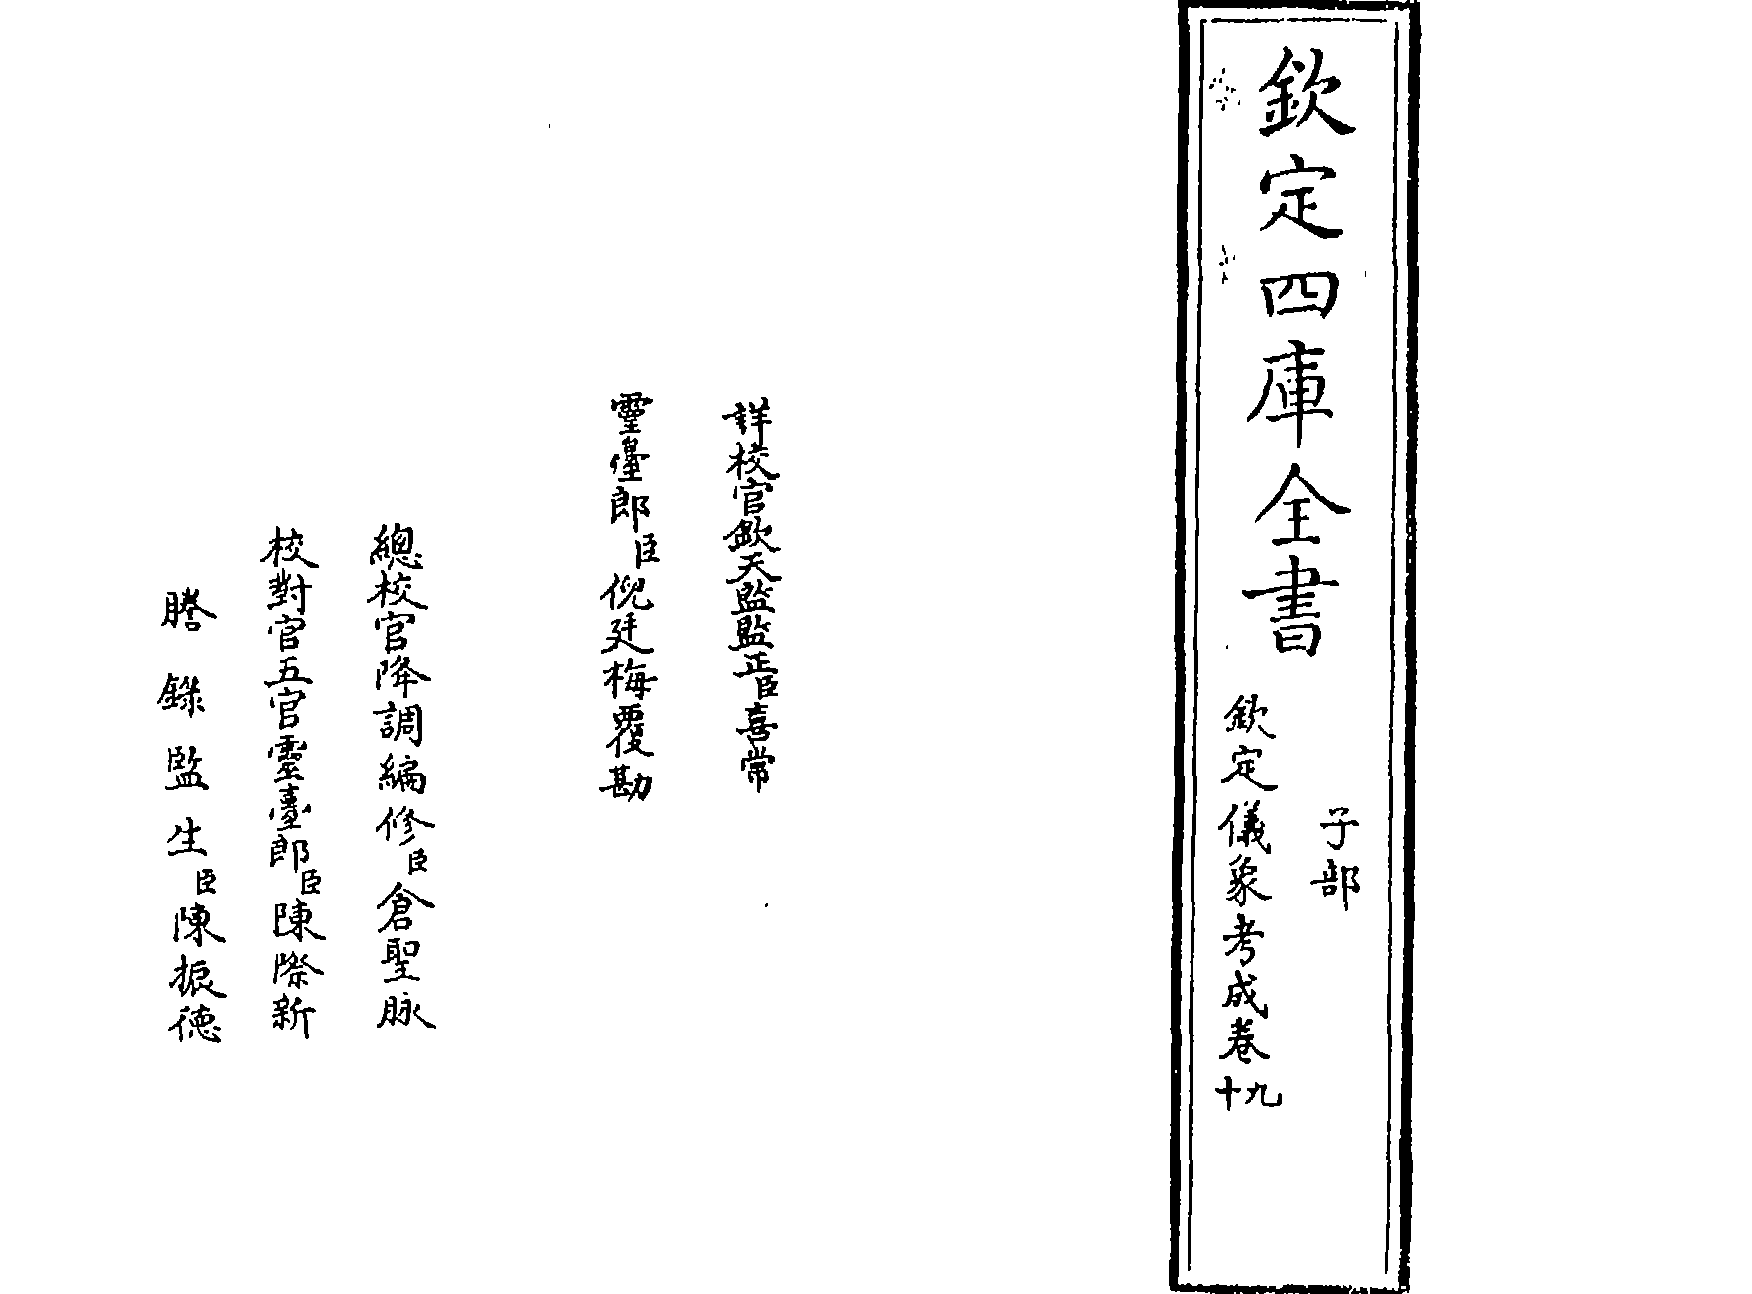
\includegraphics[width=\paperwidth,height=\paperheight,keepaspectratio]{img/0804.png}\clearpage
\begin{正文}
% ---- 册793 葉805 ----
\SetPageNumber{1}
欽定四庫全書\换行
欽定儀象考成卷九\换行
　恒星黄道經緯度表八\换行
　　黄道鶉火宫\双列{\右小列{赤道度附}\左小列{}}\换行
\char"200B\relax\换行
\char"200B\relax\换行
\char"200B\relax\换行
\char"200B\relax\换行
\char"200B\relax\换行
\char"200B\relax\换行
\char"200B\relax\换行
\char"200B\relax\换行
\char"200B\relax\换行
\char"200B\relax\换行
\char"200B\relax\换行
\char"200B\relax
\par
\end{正文}\clearpage
\嵌图{142.64pt}{201.94pt}{846.47pt}{585.91pt}{img/0808.png}
\begin{正文}
% ---- 册793 葉808 图版 ----
\SetPageNumber{2}
\插图页
\char"200B\relax\换行
\char"200B\relax\换行
\char"200B\relax\换行
\char"200B\relax\换行
\char"200B\relax\换行
\char"200B\relax\换行
\char"200B\relax\换行
\char"200B\relax\换行
\char"200B\relax\换行
\char"200B\relax\换行
\char"200B\relax\换行
\char"200B\relax\换行
\char"200B\relax\换行
\char"200B\relax\换行
\char"200B\relax\换行
\char"200B\relax
\恢复丝栏\par
\end{正文}\clearpage
\嵌图{144.63pt}{201.45pt}{842.50pt}{586.89pt}{img/0809.png}
\begin{正文}
% ---- 册793 葉809 图版 ----
\SetPageNumber{3}
\插图页
\char"200B\relax\换行
\char"200B\relax\换行
\char"200B\relax\换行
\char"200B\relax\换行
\char"200B\relax\换行
\char"200B\relax\换行
\char"200B\relax\换行
\char"200B\relax\换行
\char"200B\relax\换行
\char"200B\relax\换行
\char"200B\relax\换行
\char"200B\relax\换行
\char"200B\relax\换行
\char"200B\relax\换行
\char"200B\relax\换行
\char"200B\relax
\恢复丝栏\par
\end{正文}\clearpage
\嵌图{142.64pt}{201.00pt}{846.47pt}{587.79pt}{img/0812.png}
\begin{正文}
% ---- 册793 葉812 图版 ----
\SetPageNumber{4}
\插图页
\char"200B\relax\换行
\char"200B\relax\换行
\char"200B\relax\换行
\char"200B\relax\换行
\char"200B\relax\换行
\char"200B\relax\换行
\char"200B\relax\换行
\char"200B\relax\换行
\char"200B\relax\换行
\char"200B\relax\换行
\char"200B\relax\换行
\char"200B\relax\换行
\char"200B\relax\换行
\char"200B\relax\换行
\char"200B\relax\换行
\char"200B\relax
\恢复丝栏\par
\end{正文}\clearpage
\嵌图{148.61pt}{202.84pt}{834.55pt}{584.11pt}{img/0813.png}
\begin{正文}
% ---- 册793 葉813 图版 ----
\SetPageNumber{5}
\插图页
\char"200B\relax\换行
\char"200B\relax\换行
\char"200B\relax\换行
\char"200B\relax\换行
\char"200B\relax\换行
\char"200B\relax\换行
\char"200B\relax\换行
\char"200B\relax\换行
\char"200B\relax\换行
\char"200B\relax\换行
\char"200B\relax\换行
\char"200B\relax\换行
\char"200B\relax\换行
\char"200B\relax\换行
\char"200B\relax\换行
\char"200B\relax
\恢复丝栏\par
\end{正文}\clearpage
\嵌图{144.72pt}{202.49pt}{842.31pt}{584.82pt}{img/0816.png}
\begin{正文}
% ---- 册793 葉816 图版 ----
\SetPageNumber{6}
\插图页
\char"200B\relax\换行
\char"200B\relax\换行
\char"200B\relax\换行
\char"200B\relax\换行
\char"200B\relax\换行
\char"200B\relax\换行
\char"200B\relax\换行
\char"200B\relax\换行
\char"200B\relax\换行
\char"200B\relax\换行
\char"200B\relax\换行
\char"200B\relax\换行
\char"200B\relax\换行
\char"200B\relax\换行
\char"200B\relax\换行
\char"200B\relax
\恢复丝栏\par
\end{正文}\clearpage
\嵌图{144.72pt}{201.04pt}{842.31pt}{587.70pt}{img/0817.png}
\begin{正文}
% ---- 册793 葉817 图版 ----
\SetPageNumber{7}
\插图页
\char"200B\relax\换行
\char"200B\relax\换行
\char"200B\relax\换行
\char"200B\relax\换行
\char"200B\relax\换行
\char"200B\relax\换行
\char"200B\relax\换行
\char"200B\relax\换行
\char"200B\relax\换行
\char"200B\relax\换行
\char"200B\relax\换行
\char"200B\relax\换行
\char"200B\relax\换行
\char"200B\relax\换行
\char"200B\relax\换行
\char"200B\relax
\恢复丝栏\par
\end{正文}\clearpage
\嵌图{144.63pt}{200.98pt}{842.50pt}{587.83pt}{img/0820.png}
\begin{正文}
% ---- 册793 葉820 图版 ----
\SetPageNumber{8}
\插图页
\char"200B\relax\换行
\char"200B\relax\换行
\char"200B\relax\换行
\char"200B\relax\换行
\char"200B\relax\换行
\char"200B\relax\换行
\char"200B\relax\换行
\char"200B\relax\换行
\char"200B\relax\换行
\char"200B\relax\换行
\char"200B\relax\换行
\char"200B\relax\换行
\char"200B\relax\换行
\char"200B\relax\换行
\char"200B\relax\换行
\char"200B\relax
\恢复丝栏\par
\end{正文}\clearpage
\嵌图{144.63pt}{200.96pt}{842.50pt}{587.87pt}{img/0821.png}
\begin{正文}
% ---- 册793 葉821 图版 ----
\SetPageNumber{9}
\插图页
\char"200B\relax\换行
\char"200B\relax\换行
\char"200B\relax\换行
\char"200B\relax\换行
\char"200B\relax\换行
\char"200B\relax\换行
\char"200B\relax\换行
\char"200B\relax\换行
\char"200B\relax\换行
\char"200B\relax\换行
\char"200B\relax\换行
\char"200B\relax\换行
\char"200B\relax\换行
\char"200B\relax\换行
\char"200B\relax\换行
\char"200B\relax
\恢复丝栏\par
\end{正文}\clearpage
\嵌图{144.68pt}{202.94pt}{842.41pt}{583.90pt}{img/0824.png}
\begin{正文}
% ---- 册793 葉824 图版 ----
\SetPageNumber{10}
\插图页
\char"200B\relax\换行
\char"200B\relax\换行
\char"200B\relax\换行
\char"200B\relax\换行
\char"200B\relax\换行
\char"200B\relax\换行
\char"200B\relax\换行
\char"200B\relax\换行
\char"200B\relax\换行
\char"200B\relax\换行
\char"200B\relax\换行
\char"200B\relax\换行
\char"200B\relax\换行
\char"200B\relax\换行
\char"200B\relax\换行
\char"200B\relax
\恢复丝栏\par
\end{正文}\clearpage
\嵌图{144.68pt}{201.98pt}{842.41pt}{585.83pt}{img/0825.png}
\begin{正文}
% ---- 册793 葉825 图版 ----
\SetPageNumber{11}
\插图页
\char"200B\relax\换行
\char"200B\relax\换行
\char"200B\relax\换行
\char"200B\relax\换行
\char"200B\relax\换行
\char"200B\relax\换行
\char"200B\relax\换行
\char"200B\relax\换行
\char"200B\relax\换行
\char"200B\relax\换行
\char"200B\relax\换行
\char"200B\relax\换行
\char"200B\relax\换行
\char"200B\relax\换行
\char"200B\relax\换行
\char"200B\relax
\恢复丝栏\par
\end{正文}\clearpage
\嵌图{144.68pt}{202.94pt}{842.41pt}{583.92pt}{img/0828.png}
\begin{正文}
% ---- 册793 葉828 图版 ----
\SetPageNumber{12}
\插图页
\char"200B\relax\换行
\char"200B\relax\换行
\char"200B\relax\换行
\char"200B\relax\换行
\char"200B\relax\换行
\char"200B\relax\换行
\char"200B\relax\换行
\char"200B\relax\换行
\char"200B\relax\换行
\char"200B\relax\换行
\char"200B\relax\换行
\char"200B\relax\换行
\char"200B\relax\换行
\char"200B\relax\换行
\char"200B\relax\换行
\char"200B\relax
\恢复丝栏\par
\end{正文}\clearpage
\嵌图{144.68pt}{200.04pt}{842.41pt}{589.71pt}{img/0829.png}
\begin{正文}
% ---- 册793 葉829 图版 ----
\SetPageNumber{13}
\插图页
\char"200B\relax\换行
\char"200B\relax\换行
\char"200B\relax\换行
\char"200B\relax\换行
\char"200B\relax\换行
\char"200B\relax\换行
\char"200B\relax\换行
\char"200B\relax\换行
\char"200B\relax\换行
\char"200B\relax\换行
\char"200B\relax\换行
\char"200B\relax\换行
\char"200B\relax\换行
\char"200B\relax\换行
\char"200B\relax\换行
\char"200B\relax
\恢复丝栏\par
\end{正文}\clearpage
\嵌图{144.63pt}{202.94pt}{842.50pt}{583.92pt}{img/0832.png}
\begin{正文}
% ---- 册793 葉832 图版 ----
\SetPageNumber{14}
\插图页
\char"200B\relax\换行
\char"200B\relax\换行
\char"200B\relax\换行
\char"200B\relax\换行
\char"200B\relax\换行
\char"200B\relax\换行
\char"200B\relax\换行
\char"200B\relax\换行
\char"200B\relax\换行
\char"200B\relax\换行
\char"200B\relax\换行
\char"200B\relax\换行
\char"200B\relax\换行
\char"200B\relax\换行
\char"200B\relax\换行
\char"200B\relax
\恢复丝栏\par
\end{正文}\clearpage
\嵌图{144.63pt}{200.51pt}{842.50pt}{588.76pt}{img/0833.png}
\begin{正文}
% ---- 册793 葉833 图版 ----
\SetPageNumber{15}
\插图页
\char"200B\relax\换行
\char"200B\relax\换行
\char"200B\relax\换行
\char"200B\relax\换行
\char"200B\relax\换行
\char"200B\relax\换行
\char"200B\relax\换行
\char"200B\relax\换行
\char"200B\relax\换行
\char"200B\relax\换行
\char"200B\relax\换行
\char"200B\relax\换行
\char"200B\relax\换行
\char"200B\relax\换行
\char"200B\relax\换行
\char"200B\relax
\恢复丝栏\par
\end{正文}\clearpage
\嵌图{144.63pt}{201.51pt}{842.50pt}{586.77pt}{img/0836.png}
\begin{正文}
% ---- 册793 葉836 图版 ----
\SetPageNumber{16}
\插图页
\char"200B\relax\换行
\char"200B\relax\换行
\char"200B\relax\换行
\char"200B\relax\换行
\char"200B\relax\换行
\char"200B\relax\换行
\char"200B\relax\换行
\char"200B\relax\换行
\char"200B\relax\换行
\char"200B\relax\换行
\char"200B\relax\换行
\char"200B\relax\换行
\char"200B\relax\换行
\char"200B\relax\换行
\char"200B\relax\换行
\char"200B\relax
\恢复丝栏\par
\end{正文}\clearpage
\嵌图{146.62pt}{201.91pt}{838.53pt}{585.98pt}{img/0837.png}
\begin{正文}
% ---- 册793 葉837 图版 ----
\SetPageNumber{17}
\插图页
\char"200B\relax\换行
\char"200B\relax\换行
\char"200B\relax\换行
\char"200B\relax\换行
\char"200B\relax\换行
\char"200B\relax\换行
\char"200B\relax\换行
\char"200B\relax\换行
\char"200B\relax\换行
\char"200B\relax\换行
\char"200B\relax\换行
\char"200B\relax\换行
\char"200B\relax\换行
\char"200B\relax\换行
\char"200B\relax\换行
\char"200B\relax
\恢复丝栏\par
\end{正文}\clearpage
\嵌图{142.64pt}{201.50pt}{846.47pt}{586.78pt}{img/0840.png}
\begin{正文}
% ---- 册793 葉840 图版 ----
\SetPageNumber{18}
\插图页
\char"200B\relax\换行
\char"200B\relax\换行
\char"200B\relax\换行
\char"200B\relax\换行
\char"200B\relax\换行
\char"200B\relax\换行
\char"200B\relax\换行
\char"200B\relax\换行
\char"200B\relax\换行
\char"200B\relax\换行
\char"200B\relax\换行
\char"200B\relax\换行
\char"200B\relax\换行
\char"200B\relax\换行
\char"200B\relax\换行
\char"200B\relax
\恢复丝栏\par
\end{正文}\clearpage
\嵌图{142.64pt}{201.01pt}{846.47pt}{587.77pt}{img/0841.png}
\begin{正文}
% ---- 册793 葉841 图版 ----
\SetPageNumber{19}
\插图页
\char"200B\relax\换行
\char"200B\relax\换行
\char"200B\relax\换行
\char"200B\relax\换行
\char"200B\relax\换行
\char"200B\relax\换行
\char"200B\relax\换行
\char"200B\relax\换行
\char"200B\relax\换行
\char"200B\relax\换行
\char"200B\relax\换行
\char"200B\relax\换行
\char"200B\relax\换行
\char"200B\relax\换行
\char"200B\relax\换行
\char"200B\relax
\恢复丝栏\par
\end{正文}\clearpage
\嵌图{146.62pt}{200.02pt}{838.53pt}{589.74pt}{img/0844.png}
\begin{正文}
% ---- 册793 葉844 图版 ----
\SetPageNumber{20}
\插图页
\char"200B\relax\换行
\char"200B\relax\换行
\char"200B\relax\换行
\char"200B\relax\换行
\char"200B\relax\换行
\char"200B\relax\换行
\char"200B\relax\换行
\char"200B\relax\换行
\char"200B\relax\换行
\char"200B\relax\换行
\char"200B\relax\换行
\char"200B\relax\换行
\char"200B\relax\换行
\char"200B\relax\换行
\char"200B\relax\换行
\char"200B\relax
\恢复丝栏\par
\end{正文}\clearpage
\嵌图{142.64pt}{202.82pt}{846.47pt}{584.14pt}{img/0845.png}
\begin{正文}
% ---- 册793 葉845 图版 ----
\SetPageNumber{21}
\插图页
\char"200B\relax\换行
\char"200B\relax\换行
\char"200B\relax\换行
\char"200B\relax\换行
\char"200B\relax\换行
\char"200B\relax\换行
\char"200B\relax\换行
\char"200B\relax\换行
\char"200B\relax\换行
\char"200B\relax\换行
\char"200B\relax\换行
\char"200B\relax\换行
\char"200B\relax\换行
\char"200B\relax\换行
\char"200B\relax\换行
\char"200B\relax
\恢复丝栏\par
\end{正文}\clearpage
\嵌图{146.62pt}{201.02pt}{838.53pt}{587.76pt}{img/0848.png}
\begin{正文}
% ---- 册793 葉848 图版 ----
\SetPageNumber{22}
\插图页
\char"200B\relax\换行
\char"200B\relax\换行
\char"200B\relax\换行
\char"200B\relax\换行
\char"200B\relax\换行
\char"200B\relax\换行
\char"200B\relax\换行
\char"200B\relax\换行
\char"200B\relax\换行
\char"200B\relax\换行
\char"200B\relax\换行
\char"200B\relax\换行
\char"200B\relax\换行
\char"200B\relax\换行
\char"200B\relax\换行
\char"200B\relax
\恢复丝栏\par
\end{正文}\clearpage
\嵌图{142.64pt}{199.59pt}{846.47pt}{590.61pt}{img/0849.png}
\begin{正文}
% ---- 册793 葉849 图版 ----
\SetPageNumber{23}
\插图页
\char"200B\relax\换行
\char"200B\relax\换行
\char"200B\relax\换行
\char"200B\relax\换行
\char"200B\relax\换行
\char"200B\relax\换行
\char"200B\relax\换行
\char"200B\relax\换行
\char"200B\relax\换行
\char"200B\relax\换行
\char"200B\relax\换行
\char"200B\relax\换行
\char"200B\relax\换行
\char"200B\relax\换行
\char"200B\relax\换行
\char"200B\relax
\恢复丝栏\par
\end{正文}\clearpage
\嵌图{150.30pt}{198.15pt}{831.15pt}{593.49pt}{img/0852.png}
\begin{正文}
% ---- 册793 葉852 图版 ----
\SetPageNumber{24}
\插图页
\char"200B\relax\换行
\char"200B\relax\换行
\char"200B\relax\换行
\char"200B\relax\换行
\char"200B\relax\换行
\char"200B\relax\换行
\char"200B\relax\换行
\char"200B\relax\换行
\char"200B\relax\换行
\char"200B\relax\换行
\char"200B\relax\换行
\char"200B\relax\换行
\char"200B\relax\换行
\char"200B\relax\换行
\char"200B\relax\换行
\char"200B\relax
\恢复丝栏\par
\end{正文}\clearpage
\嵌图{150.93pt}{209.28pt}{397.09pt}{583.55pt}{img/0853.png}
\begin{正文}
% ---- 册793 葉853 ----
\SetPageNumber{25}
\插图页
\char"200B\relax\换行
\char"200B\relax\换行
\char"200B\relax\换行
\char"200B\relax\换行
\char"200B\relax\换行
\char"200B\relax\换行
\char"200B\relax\换行
\char"200B\relax\换行
\恢复丝栏
\char"200B\relax\换行
\char"200B\relax\换行
\char"200B\relax\换行
\char"200B\relax\换行
\char"200B\relax\换行
\char"200B\relax\换行
\char"200B\relax\换行
欽定儀象考成卷九
\par

% ======== 卷十（8行21字）========
\par\end{正文}\clearpage
\chapter*{欽定儀象考成卷十}
\begin{正文}
% ---- 册793 葉856 ----
\SetPageNumber{1}
欽定四庫全書\换行
欽定儀象考成卷十\换行
　恒星黄道經緯度表九\换行
　　黄道鶉尾宫\双列{\右小列{赤道度附}\左小列{}}\换行
\char"200B\relax\换行
\char"200B\relax\换行
\char"200B\relax\换行
\char"200B\relax\换行
\char"200B\relax\换行
\char"200B\relax\换行
\char"200B\relax\换行
\char"200B\relax\换行
\char"200B\relax\换行
\char"200B\relax\换行
\char"200B\relax\换行
\char"200B\relax
\par
\end{正文}\clearpage
\嵌图{144.63pt}{201.50pt}{842.50pt}{586.80pt}{img/0857.png}
\begin{正文}
% ---- 册793 葉857 图版 ----
\SetPageNumber{2}
\插图页
\char"200B\relax\换行
\char"200B\relax\换行
\char"200B\relax\换行
\char"200B\relax\换行
\char"200B\relax\换行
\char"200B\relax\换行
\char"200B\relax\换行
\char"200B\relax\换行
\char"200B\relax\换行
\char"200B\relax\换行
\char"200B\relax\换行
\char"200B\relax\换行
\char"200B\relax\换行
\char"200B\relax\换行
\char"200B\relax\换行
\char"200B\relax
\恢复丝栏\par
\end{正文}\clearpage
\嵌图{144.63pt}{201.53pt}{842.50pt}{586.74pt}{img/0860.png}
\begin{正文}
% ---- 册793 葉860 图版 ----
\SetPageNumber{3}
\插图页
\char"200B\relax\换行
\char"200B\relax\换行
\char"200B\relax\换行
\char"200B\relax\换行
\char"200B\relax\换行
\char"200B\relax\换行
\char"200B\relax\换行
\char"200B\relax\换行
\char"200B\relax\换行
\char"200B\relax\换行
\char"200B\relax\换行
\char"200B\relax\换行
\char"200B\relax\换行
\char"200B\relax\换行
\char"200B\relax\换行
\char"200B\relax
\恢复丝栏\par
\end{正文}\clearpage
\嵌图{146.62pt}{201.46pt}{838.53pt}{586.87pt}{img/0861.png}
\begin{正文}
% ---- 册793 葉861 图版 ----
\SetPageNumber{4}
\插图页
\char"200B\relax\换行
\char"200B\relax\换行
\char"200B\relax\换行
\char"200B\relax\换行
\char"200B\relax\换行
\char"200B\relax\换行
\char"200B\relax\换行
\char"200B\relax\换行
\char"200B\relax\换行
\char"200B\relax\换行
\char"200B\relax\换行
\char"200B\relax\换行
\char"200B\relax\换行
\char"200B\relax\换行
\char"200B\relax\换行
\char"200B\relax
\恢复丝栏\par
\end{正文}\clearpage
\嵌图{146.56pt}{201.05pt}{838.64pt}{587.69pt}{img/0864.png}
\begin{正文}
% ---- 册793 葉864 图版 ----
\SetPageNumber{5}
\插图页
\char"200B\relax\换行
\char"200B\relax\换行
\char"200B\relax\换行
\char"200B\relax\换行
\char"200B\relax\换行
\char"200B\relax\换行
\char"200B\relax\换行
\char"200B\relax\换行
\char"200B\relax\换行
\char"200B\relax\换行
\char"200B\relax\换行
\char"200B\relax\换行
\char"200B\relax\换行
\char"200B\relax\换行
\char"200B\relax\换行
\char"200B\relax
\恢复丝栏\par
\end{正文}\clearpage
\嵌图{146.56pt}{201.50pt}{838.64pt}{586.78pt}{img/0865.png}
\begin{正文}
% ---- 册793 葉865 图版 ----
\SetPageNumber{6}
\插图页
\char"200B\relax\换行
\char"200B\relax\换行
\char"200B\relax\换行
\char"200B\relax\换行
\char"200B\relax\换行
\char"200B\relax\换行
\char"200B\relax\换行
\char"200B\relax\换行
\char"200B\relax\换行
\char"200B\relax\换行
\char"200B\relax\换行
\char"200B\relax\换行
\char"200B\relax\换行
\char"200B\relax\换行
\char"200B\relax\换行
\char"200B\relax
\恢复丝栏\par
\end{正文}\clearpage
\嵌图{144.63pt}{200.09pt}{842.50pt}{589.60pt}{img/0868.png}
\begin{正文}
% ---- 册793 葉868 图版 ----
\SetPageNumber{7}
\插图页
\char"200B\relax\换行
\char"200B\relax\换行
\char"200B\relax\换行
\char"200B\relax\换行
\char"200B\relax\换行
\char"200B\relax\换行
\char"200B\relax\换行
\char"200B\relax\换行
\char"200B\relax\换行
\char"200B\relax\换行
\char"200B\relax\换行
\char"200B\relax\换行
\char"200B\relax\换行
\char"200B\relax\换行
\char"200B\relax\换行
\char"200B\relax
\恢复丝栏\par
\end{正文}\clearpage
\嵌图{146.62pt}{200.51pt}{838.53pt}{588.76pt}{img/0869.png}
\begin{正文}
% ---- 册793 葉869 图版 ----
\SetPageNumber{8}
\插图页
\char"200B\relax\换行
\char"200B\relax\换行
\char"200B\relax\换行
\char"200B\relax\换行
\char"200B\relax\换行
\char"200B\relax\换行
\char"200B\relax\换行
\char"200B\relax\换行
\char"200B\relax\换行
\char"200B\relax\换行
\char"200B\relax\换行
\char"200B\relax\换行
\char"200B\relax\换行
\char"200B\relax\换行
\char"200B\relax\换行
\char"200B\relax
\恢复丝栏\par
\end{正文}\clearpage
\嵌图{144.63pt}{199.14pt}{842.50pt}{591.50pt}{img/0872.png}
\begin{正文}
% ---- 册793 葉872 图版 ----
\SetPageNumber{9}
\插图页
\char"200B\relax\换行
\char"200B\relax\换行
\char"200B\relax\换行
\char"200B\relax\换行
\char"200B\relax\换行
\char"200B\relax\换行
\char"200B\relax\换行
\char"200B\relax\换行
\char"200B\relax\换行
\char"200B\relax\换行
\char"200B\relax\换行
\char"200B\relax\换行
\char"200B\relax\换行
\char"200B\relax\换行
\char"200B\relax\换行
\char"200B\relax
\恢复丝栏\par
\end{正文}\clearpage
\嵌图{146.62pt}{201.49pt}{838.53pt}{586.81pt}{img/0873.png}
\begin{正文}
% ---- 册793 葉873 图版 ----
\SetPageNumber{10}
\插图页
\char"200B\relax\换行
\char"200B\relax\换行
\char"200B\relax\换行
\char"200B\relax\换行
\char"200B\relax\换行
\char"200B\relax\换行
\char"200B\relax\换行
\char"200B\relax\换行
\char"200B\relax\换行
\char"200B\relax\换行
\char"200B\relax\换行
\char"200B\relax\换行
\char"200B\relax\换行
\char"200B\relax\换行
\char"200B\relax\换行
\char"200B\relax
\恢复丝栏\par
\end{正文}\clearpage
\嵌图{144.63pt}{200.51pt}{842.50pt}{588.77pt}{img/0876.png}
\begin{正文}
% ---- 册793 葉876 图版 ----
\SetPageNumber{11}
\插图页
\char"200B\relax\换行
\char"200B\relax\换行
\char"200B\relax\换行
\char"200B\relax\换行
\char"200B\relax\换行
\char"200B\relax\换行
\char"200B\relax\换行
\char"200B\relax\换行
\char"200B\relax\换行
\char"200B\relax\换行
\char"200B\relax\换行
\char"200B\relax\换行
\char"200B\relax\换行
\char"200B\relax\换行
\char"200B\relax\换行
\char"200B\relax
\恢复丝栏\par
\end{正文}\clearpage
\嵌图{146.62pt}{199.08pt}{838.53pt}{591.64pt}{img/0877.png}
\begin{正文}
% ---- 册793 葉877 图版 ----
\SetPageNumber{12}
\插图页
\char"200B\relax\换行
\char"200B\relax\换行
\char"200B\relax\换行
\char"200B\relax\换行
\char"200B\relax\换行
\char"200B\relax\换行
\char"200B\relax\换行
\char"200B\relax\换行
\char"200B\relax\换行
\char"200B\relax\换行
\char"200B\relax\换行
\char"200B\relax\换行
\char"200B\relax\换行
\char"200B\relax\换行
\char"200B\relax\换行
\char"200B\relax
\恢复丝栏\par
\end{正文}\clearpage
\嵌图{142.68pt}{201.00pt}{846.40pt}{587.79pt}{img/0880.png}
\begin{正文}
% ---- 册793 葉880 图版 ----
\SetPageNumber{13}
\插图页
\char"200B\relax\换行
\char"200B\relax\换行
\char"200B\relax\换行
\char"200B\relax\换行
\char"200B\relax\换行
\char"200B\relax\换行
\char"200B\relax\换行
\char"200B\relax\换行
\char"200B\relax\换行
\char"200B\relax\换行
\char"200B\relax\换行
\char"200B\relax\换行
\char"200B\relax\换行
\char"200B\relax\换行
\char"200B\relax\换行
\char"200B\relax
\恢复丝栏\par
\end{正文}\clearpage
\嵌图{142.68pt}{201.96pt}{846.40pt}{585.86pt}{img/0881.png}
\begin{正文}
% ---- 册793 葉881 图版 ----
\SetPageNumber{14}
\插图页
\char"200B\relax\换行
\char"200B\relax\换行
\char"200B\relax\换行
\char"200B\relax\换行
\char"200B\relax\换行
\char"200B\relax\换行
\char"200B\relax\换行
\char"200B\relax\换行
\char"200B\relax\换行
\char"200B\relax\换行
\char"200B\relax\换行
\char"200B\relax\换行
\char"200B\relax\换行
\char"200B\relax\换行
\char"200B\relax\换行
\char"200B\relax
\恢复丝栏\par
\end{正文}\clearpage
\嵌图{144.63pt}{200.51pt}{842.50pt}{588.76pt}{img/0884.png}
\begin{正文}
% ---- 册793 葉884 图版 ----
\SetPageNumber{15}
\插图页
\char"200B\relax\换行
\char"200B\relax\换行
\char"200B\relax\换行
\char"200B\relax\换行
\char"200B\relax\换行
\char"200B\relax\换行
\char"200B\relax\换行
\char"200B\relax\换行
\char"200B\relax\换行
\char"200B\relax\换行
\char"200B\relax\换行
\char"200B\relax\换行
\char"200B\relax\换行
\char"200B\relax\换行
\char"200B\relax\换行
\char"200B\relax
\恢复丝栏\par
\end{正文}\clearpage
\嵌图{146.62pt}{201.91pt}{838.53pt}{585.98pt}{img/0885.png}
\begin{正文}
% ---- 册793 葉885 图版 ----
\SetPageNumber{16}
\插图页
\char"200B\relax\换行
\char"200B\relax\换行
\char"200B\relax\换行
\char"200B\relax\换行
\char"200B\relax\换行
\char"200B\relax\换行
\char"200B\relax\换行
\char"200B\relax\换行
\char"200B\relax\换行
\char"200B\relax\换行
\char"200B\relax\换行
\char"200B\relax\换行
\char"200B\relax\换行
\char"200B\relax\换行
\char"200B\relax\换行
\char"200B\relax
\恢复丝栏\par
\end{正文}\clearpage
\嵌图{144.63pt}{200.54pt}{842.50pt}{588.71pt}{img/0888.png}
\begin{正文}
% ---- 册793 葉888 图版 ----
\SetPageNumber{17}
\插图页
\char"200B\relax\换行
\char"200B\relax\换行
\char"200B\relax\换行
\char"200B\relax\换行
\char"200B\relax\换行
\char"200B\relax\换行
\char"200B\relax\换行
\char"200B\relax\换行
\char"200B\relax\换行
\char"200B\relax\换行
\char"200B\relax\换行
\char"200B\relax\换行
\char"200B\relax\换行
\char"200B\relax\换行
\char"200B\relax\换行
\char"200B\relax
\恢复丝栏\par
\end{正文}\clearpage
\嵌图{144.63pt}{198.65pt}{842.50pt}{592.48pt}{img/0889.png}
\begin{正文}
% ---- 册793 葉889 图版 ----
\SetPageNumber{18}
\插图页
\char"200B\relax\换行
\char"200B\relax\换行
\char"200B\relax\换行
\char"200B\relax\换行
\char"200B\relax\换行
\char"200B\relax\换行
\char"200B\relax\换行
\char"200B\relax\换行
\char"200B\relax\换行
\char"200B\relax\换行
\char"200B\relax\换行
\char"200B\relax\换行
\char"200B\relax\换行
\char"200B\relax\换行
\char"200B\relax\换行
\char"200B\relax
\恢复丝栏\par
\end{正文}\clearpage
\嵌图{145.26pt}{209.32pt}{402.76pt}{583.51pt}{img/0892.png}
\begin{正文}
% ---- 册793 葉892 ----
\SetPageNumber{19}
\插图页
\char"200B\relax\换行
\char"200B\relax\换行
\char"200B\relax\换行
\char"200B\relax\换行
\char"200B\relax\换行
\char"200B\relax\换行
\char"200B\relax\换行
\char"200B\relax\换行
\恢复丝栏
\char"200B\relax\换行
\char"200B\relax\换行
\char"200B\relax\换行
\char"200B\relax\换行
\char"200B\relax\换行
\char"200B\relax\换行
欽定儀象考成卷十\换行
\char"200B\relax
\par

% ======== 卷十一（8行21字）========
\par\end{正文}\clearpage
\chapter*{欽定儀象考成卷十一}
\begin{正文}
\end{正文}\clearpage

  % ======== 卷十四（8行21字）========
\chapter*{欽定儀象考成卷十四}
\begin{正文}
\end{正文}\clearpage
\thispagestyle{empty}\noindent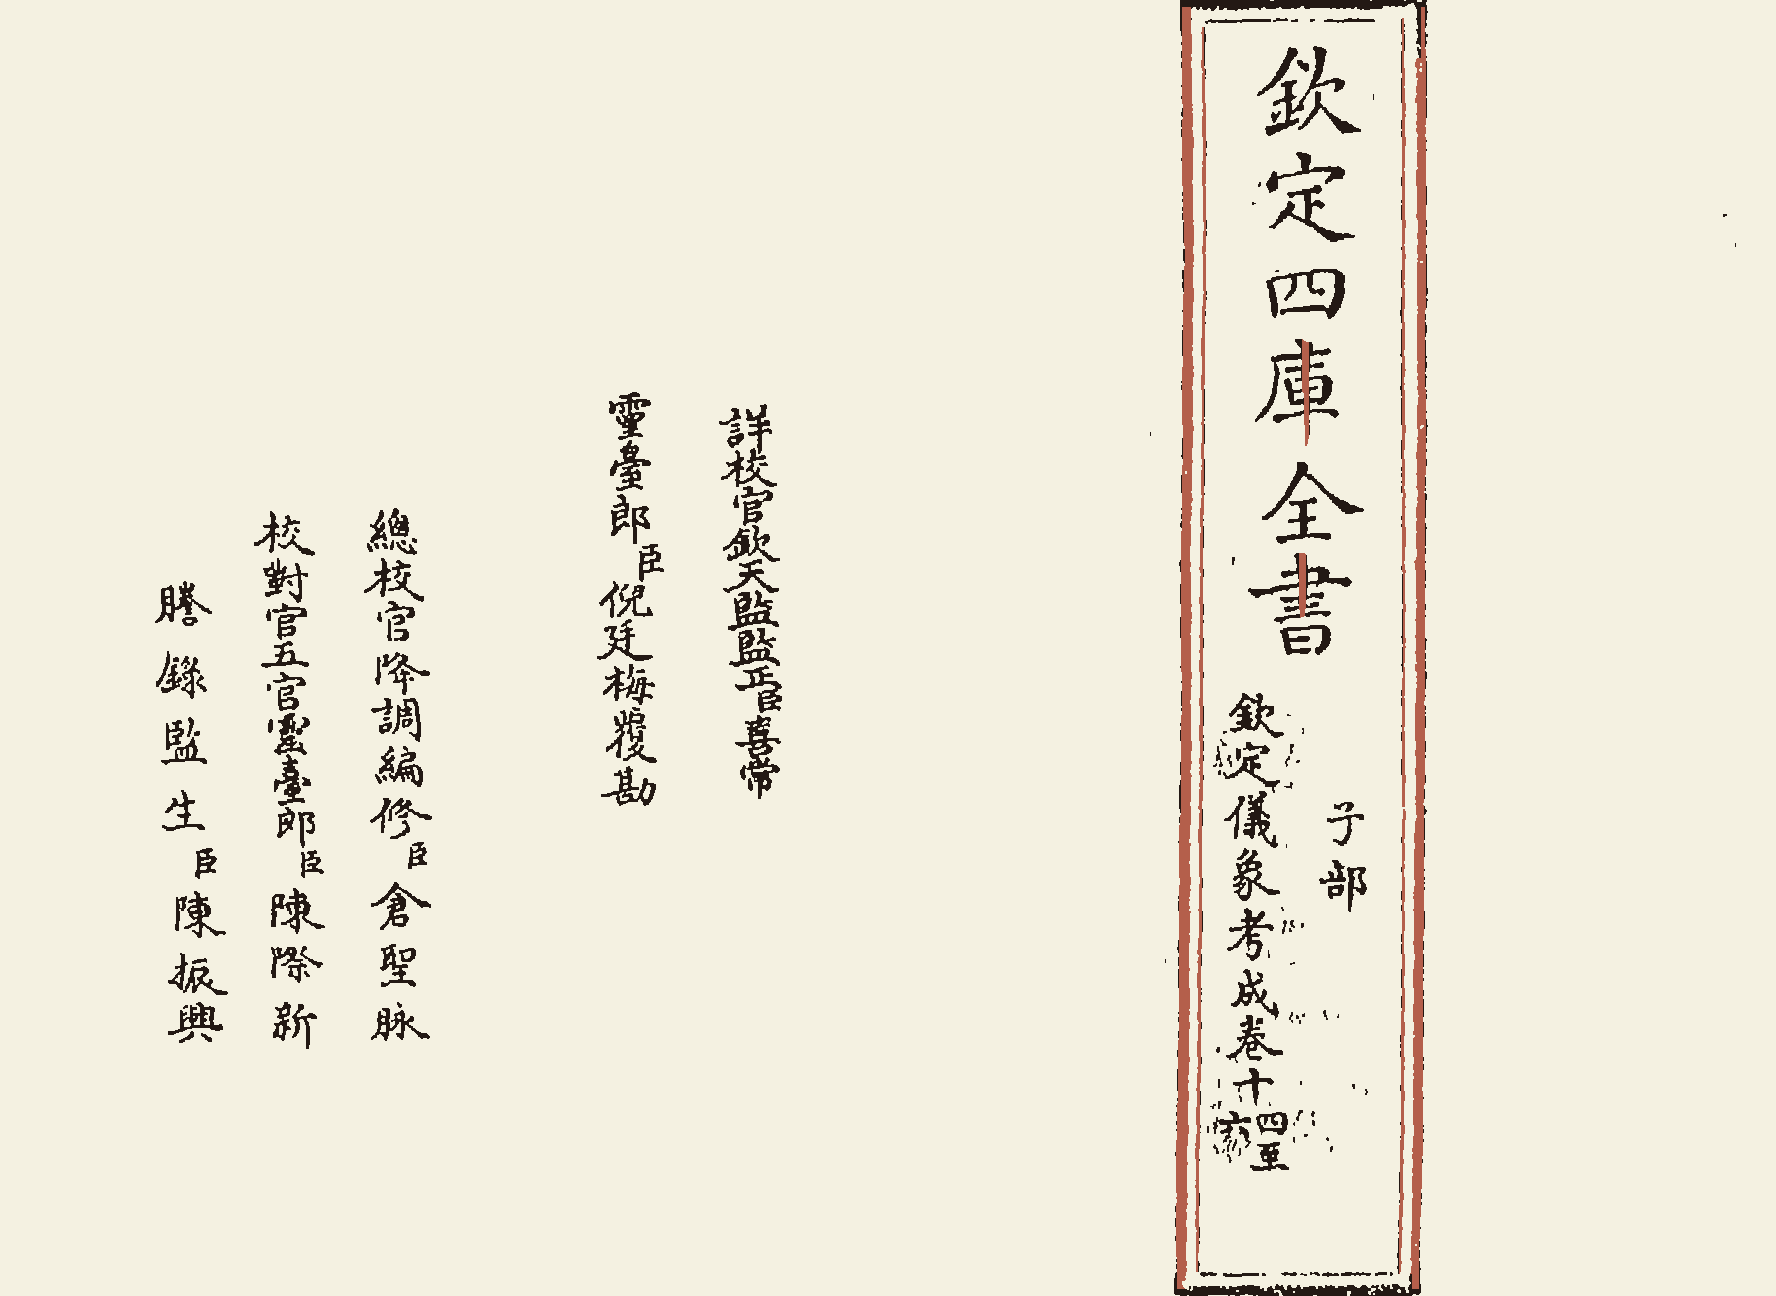
\includegraphics[width=\paperwidth,height=\paperheight,keepaspectratio]{img/1012.png}\clearpage
\begin{正文}
% ---- 册793 葉1013 ----
\SetPageNumber{1}
欽定四庫全書\换行
欽定儀象考成卷十四\换行
　恒星赤道經緯度表一\换行
　　赤道星紀宫\双列{\右小列{黄道度附}\左小列{}}\换行
\char"200B\relax\换行
\char"200B\relax\换行
\char"200B\relax\换行
\char"200B\relax\换行
\char"200B\relax\换行
\char"200B\relax\换行
\char"200B\relax\换行
\char"200B\relax\换行
\char"200B\relax\换行
\char"200B\relax\换行
\char"200B\relax\换行
\char"200B\relax
\par
\end{正文}\clearpage
\嵌图{142.64pt}{200.54pt}{846.47pt}{588.72pt}{img/1016.png}
\begin{正文}
% ---- 册793 葉1016 图版 ----
\SetPageNumber{2}
\插图页
\char"200B\relax\换行
\char"200B\relax\换行
\char"200B\relax\换行
\char"200B\relax\换行
\char"200B\relax\换行
\char"200B\relax\换行
\char"200B\relax\换行
\char"200B\relax\换行
\char"200B\relax\换行
\char"200B\relax\换行
\char"200B\relax\换行
\char"200B\relax\换行
\char"200B\relax\换行
\char"200B\relax\换行
\char"200B\relax\换行
\char"200B\relax
\恢复丝栏\par
\end{正文}\clearpage
\嵌图{148.61pt}{201.49pt}{834.55pt}{586.81pt}{img/1017.png}
\begin{正文}
% ---- 册793 葉1017 图版 ----
\SetPageNumber{3}
\插图页
\char"200B\relax\换行
\char"200B\relax\换行
\char"200B\relax\换行
\char"200B\relax\换行
\char"200B\relax\换行
\char"200B\relax\换行
\char"200B\relax\换行
\char"200B\relax\换行
\char"200B\relax\换行
\char"200B\relax\换行
\char"200B\relax\换行
\char"200B\relax\换行
\char"200B\relax\换行
\char"200B\relax\换行
\char"200B\relax\换行
\char"200B\relax
\恢复丝栏\par
\end{正文}\clearpage
\嵌图{142.72pt}{201.96pt}{846.33pt}{585.86pt}{img/1020.png}
\begin{正文}
% ---- 册793 葉1020 图版 ----
\SetPageNumber{4}
\插图页
\char"200B\relax\换行
\char"200B\relax\换行
\char"200B\relax\换行
\char"200B\relax\换行
\char"200B\relax\换行
\char"200B\relax\换行
\char"200B\relax\换行
\char"200B\relax\换行
\char"200B\relax\换行
\char"200B\relax\换行
\char"200B\relax\换行
\char"200B\relax\换行
\char"200B\relax\换行
\char"200B\relax\换行
\char"200B\relax\换行
\char"200B\relax
\恢复丝栏\par
\end{正文}\clearpage
\嵌图{144.72pt}{201.47pt}{842.31pt}{586.86pt}{img/1021.png}
\begin{正文}
% ---- 册793 葉1021 图版 ----
\SetPageNumber{5}
\插图页
\char"200B\relax\换行
\char"200B\relax\换行
\char"200B\relax\换行
\char"200B\relax\换行
\char"200B\relax\换行
\char"200B\relax\换行
\char"200B\relax\换行
\char"200B\relax\换行
\char"200B\relax\换行
\char"200B\relax\换行
\char"200B\relax\换行
\char"200B\relax\换行
\char"200B\relax\换行
\char"200B\relax\换行
\char"200B\relax\换行
\char"200B\relax
\恢复丝栏\par
\end{正文}\clearpage
\嵌图{144.63pt}{200.06pt}{842.50pt}{589.67pt}{img/1024.png}
\begin{正文}
% ---- 册793 葉1024 图版 ----
\SetPageNumber{6}
\插图页
\char"200B\relax\换行
\char"200B\relax\换行
\char"200B\relax\换行
\char"200B\relax\换行
\char"200B\relax\换行
\char"200B\relax\换行
\char"200B\relax\换行
\char"200B\relax\换行
\char"200B\relax\换行
\char"200B\relax\换行
\char"200B\relax\换行
\char"200B\relax\换行
\char"200B\relax\换行
\char"200B\relax\换行
\char"200B\relax\换行
\char"200B\relax
\恢复丝栏\par
\end{正文}\clearpage
\嵌图{144.63pt}{200.54pt}{842.50pt}{588.72pt}{img/1025.png}
\begin{正文}
% ---- 册793 葉1025 图版 ----
\SetPageNumber{7}
\插图页
\char"200B\relax\换行
\char"200B\relax\换行
\char"200B\relax\换行
\char"200B\relax\换行
\char"200B\relax\换行
\char"200B\relax\换行
\char"200B\relax\换行
\char"200B\relax\换行
\char"200B\relax\换行
\char"200B\relax\换行
\char"200B\relax\换行
\char"200B\relax\换行
\char"200B\relax\换行
\char"200B\relax\换行
\char"200B\relax\换行
\char"200B\relax
\恢复丝栏\par
\end{正文}\clearpage
\嵌图{142.72pt}{201.01pt}{846.33pt}{587.77pt}{img/1028.png}
\begin{正文}
% ---- 册793 葉1028 图版 ----
\SetPageNumber{8}
\插图页
\char"200B\relax\换行
\char"200B\relax\换行
\char"200B\relax\换行
\char"200B\relax\换行
\char"200B\relax\换行
\char"200B\relax\换行
\char"200B\relax\换行
\char"200B\relax\换行
\char"200B\relax\换行
\char"200B\relax\换行
\char"200B\relax\换行
\char"200B\relax\换行
\char"200B\relax\换行
\char"200B\relax\换行
\char"200B\relax\换行
\char"200B\relax
\恢复丝栏\par
\end{正文}\clearpage
\嵌图{144.72pt}{200.98pt}{842.31pt}{587.83pt}{img/1029.png}
\begin{正文}
% ---- 册793 葉1029 图版 ----
\SetPageNumber{9}
\插图页
\char"200B\relax\换行
\char"200B\relax\换行
\char"200B\relax\换行
\char"200B\relax\换行
\char"200B\relax\换行
\char"200B\relax\换行
\char"200B\relax\换行
\char"200B\relax\换行
\char"200B\relax\换行
\char"200B\relax\换行
\char"200B\relax\换行
\char"200B\relax\换行
\char"200B\relax\换行
\char"200B\relax\换行
\char"200B\relax\换行
\char"200B\relax
\恢复丝栏\par
\end{正文}\clearpage
\嵌图{142.64pt}{200.06pt}{846.47pt}{589.67pt}{img/1032.png}
\begin{正文}
% ---- 册793 葉1032 图版 ----
\SetPageNumber{10}
\插图页
\char"200B\relax\换行
\char"200B\relax\换行
\char"200B\relax\换行
\char"200B\relax\换行
\char"200B\relax\换行
\char"200B\relax\换行
\char"200B\relax\换行
\char"200B\relax\换行
\char"200B\relax\换行
\char"200B\relax\换行
\char"200B\relax\换行
\char"200B\relax\换行
\char"200B\relax\换行
\char"200B\relax\换行
\char"200B\relax\换行
\char"200B\relax
\恢复丝栏\par
\end{正文}\clearpage
\嵌图{144.63pt}{200.06pt}{842.50pt}{589.68pt}{img/1033.png}
\begin{正文}
% ---- 册793 葉1033 图版 ----
\SetPageNumber{11}
\插图页
\char"200B\relax\换行
\char"200B\relax\换行
\char"200B\relax\换行
\char"200B\relax\换行
\char"200B\relax\换行
\char"200B\relax\换行
\char"200B\relax\换行
\char"200B\relax\换行
\char"200B\relax\换行
\char"200B\relax\换行
\char"200B\relax\换行
\char"200B\relax\换行
\char"200B\relax\换行
\char"200B\relax\换行
\char"200B\relax\换行
\char"200B\relax
\恢复丝栏\par
\end{正文}\clearpage
\嵌图{146.62pt}{199.56pt}{838.53pt}{590.66pt}{img/1036.png}
\begin{正文}
% ---- 册793 葉1036 图版 ----
\SetPageNumber{12}
\插图页
\char"200B\relax\换行
\char"200B\relax\换行
\char"200B\relax\换行
\char"200B\relax\换行
\char"200B\relax\换行
\char"200B\relax\换行
\char"200B\relax\换行
\char"200B\relax\换行
\char"200B\relax\换行
\char"200B\relax\换行
\char"200B\relax\换行
\char"200B\relax\换行
\char"200B\relax\换行
\char"200B\relax\换行
\char"200B\relax\换行
\char"200B\relax
\恢复丝栏\par
\end{正文}\clearpage
\嵌图{144.63pt}{200.96pt}{842.50pt}{587.87pt}{img/1037.png}
\begin{正文}
% ---- 册793 葉1037 图版 ----
\SetPageNumber{13}
\插图页
\char"200B\relax\换行
\char"200B\relax\换行
\char"200B\relax\换行
\char"200B\relax\换行
\char"200B\relax\换行
\char"200B\relax\换行
\char"200B\relax\换行
\char"200B\relax\换行
\char"200B\relax\换行
\char"200B\relax\换行
\char"200B\relax\换行
\char"200B\relax\换行
\char"200B\relax\换行
\char"200B\relax\换行
\char"200B\relax\换行
\char"200B\relax
\恢复丝栏\par
\end{正文}\clearpage
\嵌图{142.68pt}{202.98pt}{846.40pt}{583.83pt}{img/1040.png}
\begin{正文}
% ---- 册793 葉1040 图版 ----
\SetPageNumber{14}
\插图页
\char"200B\relax\换行
\char"200B\relax\换行
\char"200B\relax\换行
\char"200B\relax\换行
\char"200B\relax\换行
\char"200B\relax\换行
\char"200B\relax\换行
\char"200B\relax\换行
\char"200B\relax\换行
\char"200B\relax\换行
\char"200B\relax\换行
\char"200B\relax\换行
\char"200B\relax\换行
\char"200B\relax\换行
\char"200B\relax\换行
\char"200B\relax
\恢复丝栏\par
\end{正文}\clearpage
\嵌图{144.68pt}{200.58pt}{842.41pt}{588.62pt}{img/1041.png}
\begin{正文}
% ---- 册793 葉1041 图版 ----
\SetPageNumber{15}
\插图页
\char"200B\relax\换行
\char"200B\relax\换行
\char"200B\relax\换行
\char"200B\relax\换行
\char"200B\relax\换行
\char"200B\relax\换行
\char"200B\relax\换行
\char"200B\relax\换行
\char"200B\relax\换行
\char"200B\relax\换行
\char"200B\relax\换行
\char"200B\relax\换行
\char"200B\relax\换行
\char"200B\relax\换行
\char"200B\relax\换行
\char"200B\relax
\恢复丝栏\par
\end{正文}\clearpage
\嵌图{146.62pt}{203.37pt}{838.53pt}{583.04pt}{img/1044.png}
\begin{正文}
% ---- 册793 葉1044 图版 ----
\SetPageNumber{16}
\插图页
\char"200B\relax\换行
\char"200B\relax\换行
\char"200B\relax\换行
\char"200B\relax\换行
\char"200B\relax\换行
\char"200B\relax\换行
\char"200B\relax\换行
\char"200B\relax\换行
\char"200B\relax\换行
\char"200B\relax\换行
\char"200B\relax\换行
\char"200B\relax\换行
\char"200B\relax\换行
\char"200B\relax\换行
\char"200B\relax\换行
\char"200B\relax
\恢复丝栏\par
\end{正文}\clearpage
\嵌图{142.64pt}{202.87pt}{846.47pt}{584.06pt}{img/1045.png}
\begin{正文}
% ---- 册793 葉1045 图版 ----
\SetPageNumber{17}
\插图页
\char"200B\relax\换行
\char"200B\relax\换行
\char"200B\relax\换行
\char"200B\relax\换行
\char"200B\relax\换行
\char"200B\relax\换行
\char"200B\relax\换行
\char"200B\relax\换行
\char"200B\relax\换行
\char"200B\relax\换行
\char"200B\relax\换行
\char"200B\relax\换行
\char"200B\relax\换行
\char"200B\relax\换行
\char"200B\relax\换行
\char"200B\relax
\恢复丝栏\par
\end{正文}\clearpage
\嵌图{144.72pt}{201.07pt}{842.31pt}{587.66pt}{img/1048.png}
\begin{正文}
% ---- 册793 葉1048 图版 ----
\SetPageNumber{18}
\插图页
\char"200B\relax\换行
\char"200B\relax\换行
\char"200B\relax\换行
\char"200B\relax\换行
\char"200B\relax\换行
\char"200B\relax\换行
\char"200B\relax\换行
\char"200B\relax\换行
\char"200B\relax\换行
\char"200B\relax\换行
\char"200B\relax\换行
\char"200B\relax\换行
\char"200B\relax\换行
\char"200B\relax\换行
\char"200B\relax\换行
\char"200B\relax
\恢复丝栏\par
\end{正文}\clearpage
\嵌图{142.72pt}{202.94pt}{846.33pt}{583.90pt}{img/1049.png}
\begin{正文}
% ---- 册793 葉1049 图版 ----
\SetPageNumber{19}
\插图页
\char"200B\relax\换行
\char"200B\relax\换行
\char"200B\relax\换行
\char"200B\relax\换行
\char"200B\relax\换行
\char"200B\relax\换行
\char"200B\relax\换行
\char"200B\relax\换行
\char"200B\relax\换行
\char"200B\relax\换行
\char"200B\relax\换行
\char"200B\relax\换行
\char"200B\relax\换行
\char"200B\relax\换行
\char"200B\relax\换行
\char"200B\relax
\恢复丝栏\par
\end{正文}\clearpage
\嵌图{142.72pt}{202.41pt}{846.33pt}{584.97pt}{img/1052.png}
\begin{正文}
% ---- 册793 葉1052 图版 ----
\SetPageNumber{20}
\插图页
\char"200B\relax\换行
\char"200B\relax\换行
\char"200B\relax\换行
\char"200B\relax\换行
\char"200B\relax\换行
\char"200B\relax\换行
\char"200B\relax\换行
\char"200B\relax\换行
\char"200B\relax\换行
\char"200B\relax\换行
\char"200B\relax\换行
\char"200B\relax\换行
\char"200B\relax\换行
\char"200B\relax\换行
\char"200B\relax\换行
\char"200B\relax
\恢复丝栏\par
\end{正文}\clearpage
\嵌图{142.72pt}{202.38pt}{846.33pt}{585.03pt}{img/1053.png}
\begin{正文}
% ---- 册793 葉1053 图版 ----
\SetPageNumber{21}
\插图页
\char"200B\relax\换行
\char"200B\relax\换行
\char"200B\relax\换行
\char"200B\relax\换行
\char"200B\relax\换行
\char"200B\relax\换行
\char"200B\relax\换行
\char"200B\relax\换行
\char"200B\relax\换行
\char"200B\relax\换行
\char"200B\relax\换行
\char"200B\relax\换行
\char"200B\relax\换行
\char"200B\relax\换行
\char"200B\relax\换行
\char"200B\relax
\恢复丝栏\par
\end{正文}\clearpage
\嵌图{178.71pt}{216.11pt}{660.11pt}{576.72pt}{img/1056.png}
\begin{正文}
% ---- 册793 葉1056 ----
\SetPageNumber{22}
\插图页
\char"200B\relax\换行
\char"200B\relax\换行
\char"200B\relax\换行
\char"200B\relax\换行
\char"200B\relax\换行
\char"200B\relax\换行
\char"200B\relax\换行
\char"200B\relax\换行
\恢复丝栏
\char"200B\relax\换行
\char"200B\relax\换行
\char"200B\relax\换行
\char"200B\relax\换行
\char"200B\relax\换行
\char"200B\relax\换行
\char"200B\relax\换行
欽定儀象考成卷十四
\par

% ======== 卷十五（8行21字）========
\par\end{正文}\clearpage
\chapter*{欽定儀象考成卷十五}
\begin{正文}
% ---- 册793 葉1057 ----
\SetPageNumber{1}
欽定四庫全書\换行
欽定儀象考成卷十五\换行
　恒星赤道經緯度表二\换行
　　赤道元枵宫\双列{\右小列{黄道度附}\左小列{}}\换行
\char"200B\relax\换行
\char"200B\relax\换行
\char"200B\relax\换行
\char"200B\relax\换行
\char"200B\relax\换行
\char"200B\relax\换行
\char"200B\relax\换行
\char"200B\relax\换行
\char"200B\relax\换行
\char"200B\relax\换行
\char"200B\relax\换行
\char"200B\relax
\par
\end{正文}\clearpage
\嵌图{146.67pt}{198.63pt}{838.42pt}{592.54pt}{img/1060.png}
\begin{正文}
% ---- 册793 葉1060 图版 ----
\SetPageNumber{2}
\插图页
\char"200B\relax\换行
\char"200B\relax\换行
\char"200B\relax\换行
\char"200B\relax\换行
\char"200B\relax\换行
\char"200B\relax\换行
\char"200B\relax\换行
\char"200B\relax\换行
\char"200B\relax\换行
\char"200B\relax\换行
\char"200B\relax\换行
\char"200B\relax\换行
\char"200B\relax\换行
\char"200B\relax\换行
\char"200B\relax\换行
\char"200B\relax
\恢复丝栏\par
\end{正文}\clearpage
\嵌图{144.68pt}{201.92pt}{842.41pt}{585.96pt}{img/1061.png}
\begin{正文}
% ---- 册793 葉1061 图版 ----
\SetPageNumber{3}
\插图页
\char"200B\relax\换行
\char"200B\relax\换行
\char"200B\relax\换行
\char"200B\relax\换行
\char"200B\relax\换行
\char"200B\relax\换行
\char"200B\relax\换行
\char"200B\relax\换行
\char"200B\relax\换行
\char"200B\relax\换行
\char"200B\relax\换行
\char"200B\relax\换行
\char"200B\relax\换行
\char"200B\relax\换行
\char"200B\relax\换行
\char"200B\relax
\恢复丝栏\par
\end{正文}\clearpage
\嵌图{142.64pt}{200.51pt}{846.47pt}{588.76pt}{img/1064.png}
\begin{正文}
% ---- 册793 葉1064 图版 ----
\SetPageNumber{4}
\插图页
\char"200B\relax\换行
\char"200B\relax\换行
\char"200B\relax\换行
\char"200B\relax\换行
\char"200B\relax\换行
\char"200B\relax\换行
\char"200B\relax\换行
\char"200B\relax\换行
\char"200B\relax\换行
\char"200B\relax\换行
\char"200B\relax\换行
\char"200B\relax\换行
\char"200B\relax\换行
\char"200B\relax\换行
\char"200B\relax\换行
\char"200B\relax
\恢复丝栏\par
\end{正文}\clearpage
\嵌图{144.63pt}{200.99pt}{842.50pt}{587.80pt}{img/1065.png}
\begin{正文}
% ---- 册793 葉1065 图版 ----
\SetPageNumber{5}
\插图页
\char"200B\relax\换行
\char"200B\relax\换行
\char"200B\relax\换行
\char"200B\relax\换行
\char"200B\relax\换行
\char"200B\relax\换行
\char"200B\relax\换行
\char"200B\relax\换行
\char"200B\relax\换行
\char"200B\relax\换行
\char"200B\relax\换行
\char"200B\relax\换行
\char"200B\relax\换行
\char"200B\relax\换行
\char"200B\relax\换行
\char"200B\relax
\恢复丝栏\par
\end{正文}\clearpage
\嵌图{144.63pt}{201.95pt}{842.50pt}{585.90pt}{img/1068.png}
\begin{正文}
% ---- 册793 葉1068 图版 ----
\SetPageNumber{6}
\插图页
\char"200B\relax\换行
\char"200B\relax\换行
\char"200B\relax\换行
\char"200B\relax\换行
\char"200B\relax\换行
\char"200B\relax\换行
\char"200B\relax\换行
\char"200B\relax\换行
\char"200B\relax\换行
\char"200B\relax\换行
\char"200B\relax\换行
\char"200B\relax\换行
\char"200B\relax\换行
\char"200B\relax\换行
\char"200B\relax\换行
\char"200B\relax
\恢复丝栏\par
\end{正文}\clearpage
\嵌图{146.62pt}{202.37pt}{838.53pt}{585.05pt}{img/1069.png}
\begin{正文}
% ---- 册793 葉1069 图版 ----
\SetPageNumber{7}
\插图页
\char"200B\relax\换行
\char"200B\relax\换行
\char"200B\relax\换行
\char"200B\relax\换行
\char"200B\relax\换行
\char"200B\relax\换行
\char"200B\relax\换行
\char"200B\relax\换行
\char"200B\relax\换行
\char"200B\relax\换行
\char"200B\relax\换行
\char"200B\relax\换行
\char"200B\relax\换行
\char"200B\relax\换行
\char"200B\relax\换行
\char"200B\relax
\恢复丝栏\par
\end{正文}\clearpage
\嵌图{142.68pt}{201.54pt}{846.40pt}{586.70pt}{img/1072.png}
\begin{正文}
% ---- 册793 葉1072 图版 ----
\SetPageNumber{8}
\插图页
\char"200B\relax\换行
\char"200B\relax\换行
\char"200B\relax\换行
\char"200B\relax\换行
\char"200B\relax\换行
\char"200B\relax\换行
\char"200B\relax\换行
\char"200B\relax\换行
\char"200B\relax\换行
\char"200B\relax\换行
\char"200B\relax\换行
\char"200B\relax\换行
\char"200B\relax\换行
\char"200B\relax\换行
\char"200B\relax\换行
\char"200B\relax
\恢复丝栏\par
\end{正文}\clearpage
\嵌图{146.67pt}{201.05pt}{838.42pt}{587.69pt}{img/1073.png}
\begin{正文}
% ---- 册793 葉1073 图版 ----
\SetPageNumber{9}
\插图页
\char"200B\relax\换行
\char"200B\relax\换行
\char"200B\relax\换行
\char"200B\relax\换行
\char"200B\relax\换行
\char"200B\relax\换行
\char"200B\relax\换行
\char"200B\relax\换行
\char"200B\relax\换行
\char"200B\relax\换行
\char"200B\relax\换行
\char"200B\relax\换行
\char"200B\relax\换行
\char"200B\relax\换行
\char"200B\relax\换行
\char"200B\relax
\恢复丝栏\par
\end{正文}\clearpage
\嵌图{144.63pt}{200.54pt}{842.50pt}{588.72pt}{img/1076.png}
\begin{正文}
% ---- 册793 葉1076 图版 ----
\SetPageNumber{10}
\插图页
\char"200B\relax\换行
\char"200B\relax\换行
\char"200B\relax\换行
\char"200B\relax\换行
\char"200B\relax\换行
\char"200B\relax\换行
\char"200B\relax\换行
\char"200B\relax\换行
\char"200B\relax\换行
\char"200B\relax\换行
\char"200B\relax\换行
\char"200B\relax\换行
\char"200B\relax\换行
\char"200B\relax\换行
\char"200B\relax\换行
\char"200B\relax
\恢复丝栏\par
\end{正文}\clearpage
\嵌图{144.63pt}{202.39pt}{842.50pt}{585.00pt}{img/1077.png}
\begin{正文}
% ---- 册793 葉1077 图版 ----
\SetPageNumber{11}
\插图页
\char"200B\relax\换行
\char"200B\relax\换行
\char"200B\relax\换行
\char"200B\relax\换行
\char"200B\relax\换行
\char"200B\relax\换行
\char"200B\relax\换行
\char"200B\relax\换行
\char"200B\relax\换行
\char"200B\relax\换行
\char"200B\relax\换行
\char"200B\relax\换行
\char"200B\relax\换行
\char"200B\relax\换行
\char"200B\relax\换行
\char"200B\relax
\恢复丝栏\par
\end{正文}\clearpage
\嵌图{144.68pt}{199.17pt}{842.41pt}{591.44pt}{img/1080.png}
\begin{正文}
% ---- 册793 葉1080 图版 ----
\SetPageNumber{12}
\插图页
\char"200B\relax\换行
\char"200B\relax\换行
\char"200B\relax\换行
\char"200B\relax\换行
\char"200B\relax\换行
\char"200B\relax\换行
\char"200B\relax\换行
\char"200B\relax\换行
\char"200B\relax\换行
\char"200B\relax\换行
\char"200B\relax\换行
\char"200B\relax\换行
\char"200B\relax\换行
\char"200B\relax\换行
\char"200B\relax\换行
\char"200B\relax
\恢复丝栏\par
\end{正文}\clearpage
\嵌图{146.67pt}{199.16pt}{838.42pt}{591.47pt}{img/1081.png}
\begin{正文}
% ---- 册793 葉1081 图版 ----
\SetPageNumber{13}
\插图页
\char"200B\relax\换行
\char"200B\relax\换行
\char"200B\relax\换行
\char"200B\relax\换行
\char"200B\relax\换行
\char"200B\relax\换行
\char"200B\relax\换行
\char"200B\relax\换行
\char"200B\relax\换行
\char"200B\relax\换行
\char"200B\relax\换行
\char"200B\relax\换行
\char"200B\relax\换行
\char"200B\relax\换行
\char"200B\relax\换行
\char"200B\relax
\恢复丝栏\par
\end{正文}\clearpage
\嵌图{146.62pt}{201.04pt}{838.53pt}{587.72pt}{img/1084.png}
\begin{正文}
% ---- 册793 葉1084 图版 ----
\SetPageNumber{14}
\插图页
\char"200B\relax\换行
\char"200B\relax\换行
\char"200B\relax\换行
\char"200B\relax\换行
\char"200B\relax\换行
\char"200B\relax\换行
\char"200B\relax\换行
\char"200B\relax\换行
\char"200B\relax\换行
\char"200B\relax\换行
\char"200B\relax\换行
\char"200B\relax\换行
\char"200B\relax\换行
\char"200B\relax\换行
\char"200B\relax\换行
\char"200B\relax
\恢复丝栏\par
\end{正文}\clearpage
\嵌图{144.63pt}{200.99pt}{842.50pt}{587.80pt}{img/1085.png}
\begin{正文}
% ---- 册793 葉1085 图版 ----
\SetPageNumber{15}
\插图页
\char"200B\relax\换行
\char"200B\relax\换行
\char"200B\relax\换行
\char"200B\relax\换行
\char"200B\relax\换行
\char"200B\relax\换行
\char"200B\relax\换行
\char"200B\relax\换行
\char"200B\relax\换行
\char"200B\relax\换行
\char"200B\relax\换行
\char"200B\relax\换行
\char"200B\relax\换行
\char"200B\relax\换行
\char"200B\relax\换行
\char"200B\relax
\恢复丝栏\par
\end{正文}\clearpage
\嵌图{144.63pt}{201.50pt}{842.50pt}{586.78pt}{img/1088.png}
\begin{正文}
% ---- 册793 葉1088 图版 ----
\SetPageNumber{16}
\插图页
\char"200B\relax\换行
\char"200B\relax\换行
\char"200B\relax\换行
\char"200B\relax\换行
\char"200B\relax\换行
\char"200B\relax\换行
\char"200B\relax\换行
\char"200B\relax\换行
\char"200B\relax\换行
\char"200B\relax\换行
\char"200B\relax\换行
\char"200B\relax\换行
\char"200B\relax\换行
\char"200B\relax\换行
\char"200B\relax\换行
\char"200B\relax
\恢复丝栏\par
\end{正文}\clearpage
\嵌图{142.64pt}{203.39pt}{846.47pt}{583.00pt}{img/1089.png}
\begin{正文}
% ---- 册793 葉1089 图版 ----
\SetPageNumber{17}
\插图页
\char"200B\relax\换行
\char"200B\relax\换行
\char"200B\relax\换行
\char"200B\relax\换行
\char"200B\relax\换行
\char"200B\relax\换行
\char"200B\relax\换行
\char"200B\relax\换行
\char"200B\relax\换行
\char"200B\relax\换行
\char"200B\relax\换行
\char"200B\relax\换行
\char"200B\relax\换行
\char"200B\relax\换行
\char"200B\relax\换行
\char"200B\relax
\恢复丝栏\par
\end{正文}\clearpage
\嵌图{148.61pt}{203.36pt}{834.55pt}{583.08pt}{img/1092.png}
\begin{正文}
% ---- 册793 葉1092 图版 ----
\SetPageNumber{18}
\插图页
\char"200B\relax\换行
\char"200B\relax\换行
\char"200B\relax\换行
\char"200B\relax\换行
\char"200B\relax\换行
\char"200B\relax\换行
\char"200B\relax\换行
\char"200B\relax\换行
\char"200B\relax\换行
\char"200B\relax\换行
\char"200B\relax\换行
\char"200B\relax\换行
\char"200B\relax\换行
\char"200B\relax\换行
\char"200B\relax\换行
\char"200B\relax
\恢复丝栏\par
\end{正文}\clearpage
\嵌图{142.64pt}{202.41pt}{846.47pt}{584.97pt}{img/1093.png}
\begin{正文}
% ---- 册793 葉1093 图版 ----
\SetPageNumber{19}
\插图页
\char"200B\relax\换行
\char"200B\relax\换行
\char"200B\relax\换行
\char"200B\relax\换行
\char"200B\relax\换行
\char"200B\relax\换行
\char"200B\relax\换行
\char"200B\relax\换行
\char"200B\relax\换行
\char"200B\relax\换行
\char"200B\relax\换行
\char"200B\relax\换行
\char"200B\relax\换行
\char"200B\relax\换行
\char"200B\relax\换行
\char"200B\relax
\恢复丝栏\par
\end{正文}\clearpage
\嵌图{146.56pt}{200.58pt}{838.64pt}{588.62pt}{img/1096.png}
\begin{正文}
% ---- 册793 葉1096 图版 ----
\SetPageNumber{20}
\插图页
\char"200B\relax\换行
\char"200B\relax\换行
\char"200B\relax\换行
\char"200B\relax\换行
\char"200B\relax\换行
\char"200B\relax\换行
\char"200B\relax\换行
\char"200B\relax\换行
\char"200B\relax\换行
\char"200B\relax\换行
\char"200B\relax\换行
\char"200B\relax\换行
\char"200B\relax\换行
\char"200B\relax\换行
\char"200B\relax\换行
\char"200B\relax
\恢复丝栏\par
\end{正文}\clearpage
\嵌图{144.59pt}{201.97pt}{842.59pt}{585.85pt}{img/1097.png}
\begin{正文}
% ---- 册793 葉1097 图版 ----
\SetPageNumber{21}
\插图页
\char"200B\relax\换行
\char"200B\relax\换行
\char"200B\relax\换行
\char"200B\relax\换行
\char"200B\relax\换行
\char"200B\relax\换行
\char"200B\relax\换行
\char"200B\relax\换行
\char"200B\relax\换行
\char"200B\relax\换行
\char"200B\relax\换行
\char"200B\relax\换行
\char"200B\relax\换行
\char"200B\relax\换行
\char"200B\relax\换行
\char"200B\relax
\恢复丝栏\par
\end{正文}\clearpage
\嵌图{144.63pt}{203.32pt}{842.50pt}{583.15pt}{img/1100.png}
\begin{正文}
% ---- 册793 葉1100 图版 ----
\SetPageNumber{22}
\插图页
\char"200B\relax\换行
\char"200B\relax\换行
\char"200B\relax\换行
\char"200B\relax\换行
\char"200B\relax\换行
\char"200B\relax\换行
\char"200B\relax\换行
\char"200B\relax\换行
\char"200B\relax\换行
\char"200B\relax\换行
\char"200B\relax\换行
\char"200B\relax\换行
\char"200B\relax\换行
\char"200B\relax\换行
\char"200B\relax\换行
\char"200B\relax
\恢复丝栏\par
\end{正文}\clearpage
\嵌图{140.66pt}{200.95pt}{850.45pt}{587.89pt}{img/1101.png}
\begin{正文}
% ---- 册793 葉1101 图版 ----
\SetPageNumber{23}
\插图页
\char"200B\relax\换行
\char"200B\relax\换行
\char"200B\relax\换行
\char"200B\relax\换行
\char"200B\relax\换行
\char"200B\relax\换行
\char"200B\relax\换行
\char"200B\relax\换行
\char"200B\relax\换行
\char"200B\relax\换行
\char"200B\relax\换行
\char"200B\relax\换行
\char"200B\relax\换行
\char"200B\relax\换行
\char"200B\relax\换行
\char"200B\relax
\恢复丝栏\par
\end{正文}\clearpage
\嵌图{148.42pt}{202.89pt}{834.93pt}{584.00pt}{img/1104.png}
\begin{正文}
% ---- 册793 葉1104 图版 ----
\SetPageNumber{24}
\插图页
\char"200B\relax\换行
\char"200B\relax\换行
\char"200B\relax\换行
\char"200B\relax\换行
\char"200B\relax\换行
\char"200B\relax\换行
\char"200B\relax\换行
\char"200B\relax\换行
\char"200B\relax\换行
\char"200B\relax\换行
\char"200B\relax\换行
\char"200B\relax\换行
\char"200B\relax\换行
\char"200B\relax\换行
\char"200B\relax\换行
\char"200B\relax
\恢复丝栏\par
\end{正文}\clearpage
\嵌图{165.80pt}{216.14pt}{178.15pt}{576.69pt}{img/1105.png}
\begin{正文}
% ---- 册793 葉1105 ----
\SetPageNumber{25}
\char"200B\relax\换行
\char"200B\relax\换行
\char"200B\relax\换行
\char"200B\relax\换行
\char"200B\relax\换行
\char"200B\relax\换行
\char"200B\relax\换行
\char"200B\relax\换行
\char"200B\relax\换行
\char"200B\relax\换行
\char"200B\relax\换行
\char"200B\relax\换行
\char"200B\relax\换行
\char"200B\relax\换行
\char"200B\relax\换行
欽定儀象考成卷十五
\par

% ======== 卷十六（8行21字）========
\par\end{正文}\clearpage
\chapter*{欽定儀象考成卷十六}
\begin{正文}
% ---- 册793 葉1108 ----
\SetPageNumber{1}
欽定四庫全書\换行
欽定儀象考成卷十六\换行
　恒星赤道經緯度表三\换行
　　赤道娵訾宫\双列{\右小列{黄道度附}\左小列{}}\换行
\char"200B\relax\换行
\char"200B\relax\换行
\char"200B\relax\换行
\char"200B\relax\换行
\char"200B\relax\换行
\char"200B\relax\换行
\char"200B\relax\换行
\char"200B\relax\换行
\char"200B\relax\换行
\char"200B\relax\换行
\char"200B\relax\换行
\char"200B\relax
\par
\end{正文}\clearpage
\嵌图{140.66pt}{201.44pt}{850.45pt}{586.92pt}{img/1109.png}
\begin{正文}
% ---- 册793 葉1109 图版 ----
\SetPageNumber{2}
\插图页
\char"200B\relax\换行
\char"200B\relax\换行
\char"200B\relax\换行
\char"200B\relax\换行
\char"200B\relax\换行
\char"200B\relax\换行
\char"200B\relax\换行
\char"200B\relax\换行
\char"200B\relax\换行
\char"200B\relax\换行
\char"200B\relax\换行
\char"200B\relax\换行
\char"200B\relax\换行
\char"200B\relax\换行
\char"200B\relax\换行
\char"200B\relax
\恢复丝栏\par
\end{正文}\clearpage
\嵌图{144.63pt}{200.05pt}{842.50pt}{589.69pt}{img/1112.png}
\begin{正文}
% ---- 册793 葉1112 图版 ----
\SetPageNumber{3}
\插图页
\char"200B\relax\换行
\char"200B\relax\换行
\char"200B\relax\换行
\char"200B\relax\换行
\char"200B\relax\换行
\char"200B\relax\换行
\char"200B\relax\换行
\char"200B\relax\换行
\char"200B\relax\换行
\char"200B\relax\换行
\char"200B\relax\换行
\char"200B\relax\换行
\char"200B\relax\换行
\char"200B\relax\换行
\char"200B\relax\换行
\char"200B\relax
\恢复丝栏\par
\end{正文}\clearpage
\嵌图{142.64pt}{200.55pt}{846.47pt}{588.69pt}{img/1113.png}
\begin{正文}
% ---- 册793 葉1113 图版 ----
\SetPageNumber{4}
\插图页
\char"200B\relax\换行
\char"200B\relax\换行
\char"200B\relax\换行
\char"200B\relax\换行
\char"200B\relax\换行
\char"200B\relax\换行
\char"200B\relax\换行
\char"200B\relax\换行
\char"200B\relax\换行
\char"200B\relax\换行
\char"200B\relax\换行
\char"200B\relax\换行
\char"200B\relax\换行
\char"200B\relax\换行
\char"200B\relax\换行
\char"200B\relax
\恢复丝栏\par
\end{正文}\clearpage
\嵌图{144.63pt}{200.07pt}{842.50pt}{589.64pt}{img/1116.png}
\begin{正文}
% ---- 册793 葉1116 图版 ----
\SetPageNumber{5}
\插图页
\char"200B\relax\换行
\char"200B\relax\换行
\char"200B\relax\换行
\char"200B\relax\换行
\char"200B\relax\换行
\char"200B\relax\换行
\char"200B\relax\换行
\char"200B\relax\换行
\char"200B\relax\换行
\char"200B\relax\换行
\char"200B\relax\换行
\char"200B\relax\换行
\char"200B\relax\换行
\char"200B\relax\换行
\char"200B\relax\换行
\char"200B\relax
\恢复丝栏\par
\end{正文}\clearpage
\嵌图{144.63pt}{201.00pt}{842.50pt}{587.79pt}{img/1117.png}
\begin{正文}
% ---- 册793 葉1117 图版 ----
\SetPageNumber{6}
\插图页
\char"200B\relax\换行
\char"200B\relax\换行
\char"200B\relax\换行
\char"200B\relax\换行
\char"200B\relax\换行
\char"200B\relax\换行
\char"200B\relax\换行
\char"200B\relax\换行
\char"200B\relax\换行
\char"200B\relax\换行
\char"200B\relax\换行
\char"200B\relax\换行
\char"200B\relax\换行
\char"200B\relax\换行
\char"200B\relax\换行
\char"200B\relax
\恢复丝栏\par
\end{正文}\clearpage
\嵌图{144.63pt}{202.94pt}{842.50pt}{583.90pt}{img/1120.png}
\begin{正文}
% ---- 册793 葉1120 图版 ----
\SetPageNumber{7}
\插图页
\char"200B\relax\换行
\char"200B\relax\换行
\char"200B\relax\换行
\char"200B\relax\换行
\char"200B\relax\换行
\char"200B\relax\换行
\char"200B\relax\换行
\char"200B\relax\换行
\char"200B\relax\换行
\char"200B\relax\换行
\char"200B\relax\换行
\char"200B\relax\换行
\char"200B\relax\换行
\char"200B\relax\换行
\char"200B\relax\换行
\char"200B\relax
\恢复丝栏\par
\end{正文}\clearpage
\嵌图{144.63pt}{201.50pt}{842.50pt}{586.80pt}{img/1121.png}
\begin{正文}
% ---- 册793 葉1121 图版 ----
\SetPageNumber{8}
\插图页
\char"200B\relax\换行
\char"200B\relax\换行
\char"200B\relax\换行
\char"200B\relax\换行
\char"200B\relax\换行
\char"200B\relax\换行
\char"200B\relax\换行
\char"200B\relax\换行
\char"200B\relax\换行
\char"200B\relax\换行
\char"200B\relax\换行
\char"200B\relax\换行
\char"200B\relax\换行
\char"200B\relax\换行
\char"200B\relax\换行
\char"200B\relax
\恢复丝栏\par
\end{正文}\clearpage
\嵌图{144.63pt}{200.13pt}{842.50pt}{589.52pt}{img/1124.png}
\begin{正文}
% ---- 册793 葉1124 图版 ----
\SetPageNumber{9}
\插图页
\char"200B\relax\换行
\char"200B\relax\换行
\char"200B\relax\换行
\char"200B\relax\换行
\char"200B\relax\换行
\char"200B\relax\换行
\char"200B\relax\换行
\char"200B\relax\换行
\char"200B\relax\换行
\char"200B\relax\换行
\char"200B\relax\换行
\char"200B\relax\换行
\char"200B\relax\换行
\char"200B\relax\换行
\char"200B\relax\换行
\char"200B\relax
\恢复丝栏\par
\end{正文}\clearpage
\嵌图{144.63pt}{199.61pt}{842.50pt}{590.56pt}{img/1125.png}
\begin{正文}
% ---- 册793 葉1125 图版 ----
\SetPageNumber{10}
\插图页
\char"200B\relax\换行
\char"200B\relax\换行
\char"200B\relax\换行
\char"200B\relax\换行
\char"200B\relax\换行
\char"200B\relax\换行
\char"200B\relax\换行
\char"200B\relax\换行
\char"200B\relax\换行
\char"200B\relax\换行
\char"200B\relax\换行
\char"200B\relax\换行
\char"200B\relax\换行
\char"200B\relax\换行
\char"200B\relax\换行
\char"200B\relax
\恢复丝栏\par
\end{正文}\clearpage
\嵌图{144.59pt}{201.08pt}{842.59pt}{587.63pt}{img/1128.png}
\begin{正文}
% ---- 册793 葉1128 图版 ----
\SetPageNumber{11}
\插图页
\char"200B\relax\换行
\char"200B\relax\换行
\char"200B\relax\换行
\char"200B\relax\换行
\char"200B\relax\换行
\char"200B\relax\换行
\char"200B\relax\换行
\char"200B\relax\换行
\char"200B\relax\换行
\char"200B\relax\换行
\char"200B\relax\换行
\char"200B\relax\换行
\char"200B\relax\换行
\char"200B\relax\换行
\char"200B\relax\换行
\char"200B\relax
\恢复丝栏\par
\end{正文}\clearpage
\嵌图{146.56pt}{199.60pt}{838.64pt}{590.59pt}{img/1129.png}
\begin{正文}
% ---- 册793 葉1129 图版 ----
\SetPageNumber{12}
\插图页
\char"200B\relax\换行
\char"200B\relax\换行
\char"200B\relax\换行
\char"200B\relax\换行
\char"200B\relax\换行
\char"200B\relax\换行
\char"200B\relax\换行
\char"200B\relax\换行
\char"200B\relax\换行
\char"200B\relax\换行
\char"200B\relax\换行
\char"200B\relax\换行
\char"200B\relax\换行
\char"200B\relax\换行
\char"200B\relax\换行
\char"200B\relax
\恢复丝栏\par
\end{正文}\clearpage
\嵌图{144.63pt}{201.50pt}{842.50pt}{586.80pt}{img/1132.png}
\begin{正文}
% ---- 册793 葉1132 图版 ----
\SetPageNumber{13}
\插图页
\char"200B\relax\换行
\char"200B\relax\换行
\char"200B\relax\换行
\char"200B\relax\换行
\char"200B\relax\换行
\char"200B\relax\换行
\char"200B\relax\换行
\char"200B\relax\换行
\char"200B\relax\换行
\char"200B\relax\换行
\char"200B\relax\换行
\char"200B\relax\换行
\char"200B\relax\换行
\char"200B\relax\换行
\char"200B\relax\换行
\char"200B\relax
\恢复丝栏\par
\end{正文}\clearpage
\嵌图{142.64pt}{201.47pt}{846.47pt}{586.86pt}{img/1133.png}
\begin{正文}
% ---- 册793 葉1133 图版 ----
\SetPageNumber{14}
\插图页
\char"200B\relax\换行
\char"200B\relax\换行
\char"200B\relax\换行
\char"200B\relax\换行
\char"200B\relax\换行
\char"200B\relax\换行
\char"200B\relax\换行
\char"200B\relax\换行
\char"200B\relax\换行
\char"200B\relax\换行
\char"200B\relax\换行
\char"200B\relax\换行
\char"200B\relax\换行
\char"200B\relax\换行
\char"200B\relax\换行
\char"200B\relax
\恢复丝栏\par
\end{正文}\clearpage
\嵌图{144.63pt}{204.36pt}{842.50pt}{581.07pt}{img/1136.png}
\begin{正文}
% ---- 册793 葉1136 图版 ----
\SetPageNumber{15}
\插图页
\char"200B\relax\换行
\char"200B\relax\换行
\char"200B\relax\换行
\char"200B\relax\换行
\char"200B\relax\换行
\char"200B\relax\换行
\char"200B\relax\换行
\char"200B\relax\换行
\char"200B\relax\换行
\char"200B\relax\换行
\char"200B\relax\换行
\char"200B\relax\换行
\char"200B\relax\换行
\char"200B\relax\换行
\char"200B\relax\换行
\char"200B\relax
\恢复丝栏\par
\end{正文}\clearpage
\嵌图{146.62pt}{201.06pt}{838.53pt}{587.67pt}{img/1137.png}
\begin{正文}
% ---- 册793 葉1137 图版 ----
\SetPageNumber{16}
\插图页
\char"200B\relax\换行
\char"200B\relax\换行
\char"200B\relax\换行
\char"200B\relax\换行
\char"200B\relax\换行
\char"200B\relax\换行
\char"200B\relax\换行
\char"200B\relax\换行
\char"200B\relax\换行
\char"200B\relax\换行
\char"200B\relax\换行
\char"200B\relax\换行
\char"200B\relax\换行
\char"200B\relax\换行
\char"200B\relax\换行
\char"200B\relax
\恢复丝栏\par
\end{正文}\clearpage
\嵌图{146.56pt}{204.34pt}{838.64pt}{581.11pt}{img/1140.png}
\begin{正文}
% ---- 册793 葉1140 图版 ----
\SetPageNumber{17}
\插图页
\char"200B\relax\换行
\char"200B\relax\换行
\char"200B\relax\换行
\char"200B\relax\换行
\char"200B\relax\换行
\char"200B\relax\换行
\char"200B\relax\换行
\char"200B\relax\换行
\char"200B\relax\换行
\char"200B\relax\换行
\char"200B\relax\换行
\char"200B\relax\换行
\char"200B\relax\换行
\char"200B\relax\换行
\char"200B\relax\换行
\char"200B\relax
\恢复丝栏\par
\end{正文}\clearpage
\嵌图{146.56pt}{202.91pt}{838.64pt}{583.97pt}{img/1141.png}
\begin{正文}
% ---- 册793 葉1141 图版 ----
\SetPageNumber{18}
\插图页
\char"200B\relax\换行
\char"200B\relax\换行
\char"200B\relax\换行
\char"200B\relax\换行
\char"200B\relax\换行
\char"200B\relax\换行
\char"200B\relax\换行
\char"200B\relax\换行
\char"200B\relax\换行
\char"200B\relax\换行
\char"200B\relax\换行
\char"200B\relax\换行
\char"200B\relax\换行
\char"200B\relax\换行
\char"200B\relax\换行
\char"200B\relax
\恢复丝栏\par
\end{正文}\clearpage
\嵌图{144.63pt}{201.05pt}{842.50pt}{587.69pt}{img/1144.png}
\begin{正文}
% ---- 册793 葉1144 图版 ----
\SetPageNumber{19}
\插图页
\char"200B\relax\换行
\char"200B\relax\换行
\char"200B\relax\换行
\char"200B\relax\换行
\char"200B\relax\换行
\char"200B\relax\换行
\char"200B\relax\换行
\char"200B\relax\换行
\char"200B\relax\换行
\char"200B\relax\换行
\char"200B\relax\换行
\char"200B\relax\换行
\char"200B\relax\换行
\char"200B\relax\换行
\char"200B\relax\换行
\char"200B\relax
\恢复丝栏\par
\end{正文}\clearpage
\嵌图{144.63pt}{202.48pt}{842.50pt}{584.83pt}{img/1145.png}
\begin{正文}
% ---- 册793 葉1145 图版 ----
\SetPageNumber{20}
\插图页
\char"200B\relax\换行
\char"200B\relax\换行
\char"200B\relax\换行
\char"200B\relax\换行
\char"200B\relax\换行
\char"200B\relax\换行
\char"200B\relax\换行
\char"200B\relax\换行
\char"200B\relax\换行
\char"200B\relax\换行
\char"200B\relax\换行
\char"200B\relax\换行
\char"200B\relax\换行
\char"200B\relax\换行
\char"200B\relax\换行
\char"200B\relax
\恢复丝栏\par
\end{正文}\clearpage
\嵌图{150.52pt}{201.99pt}{830.72pt}{585.82pt}{img/1148.png}
\begin{正文}
% ---- 册793 葉1148 图版 ----
\SetPageNumber{21}
\插图页
\char"200B\relax\换行
\char"200B\relax\换行
\char"200B\relax\换行
\char"200B\relax\换行
\char"200B\relax\换行
\char"200B\relax\换行
\char"200B\relax\换行
\char"200B\relax\换行
\char"200B\relax\换行
\char"200B\relax\换行
\char"200B\relax\换行
\char"200B\relax\换行
\char"200B\relax\换行
\char"200B\relax\换行
\char"200B\relax\换行
\char"200B\relax
\恢复丝栏\par
% ---- 册793 葉1149 ----
\char"200B\relax\换行
\char"200B\relax\换行
\char"200B\relax\换行
\char"200B\relax\换行
\char"200B\relax\换行
\char"200B\relax\换行
\char"200B\relax\换行
\char"200B\relax\换行
\char"200B\relax\换行
\char"200B\relax\换行
\char"200B\relax\换行
\char"200B\relax\换行
\char"200B\relax\换行
\char"200B\relax\换行
\char"200B\relax\换行
欽定儀象考成卷十六
\par

\par\end{正文}\clearpage

  \input{parts/part11}
  \thispagestyle{empty}\noindent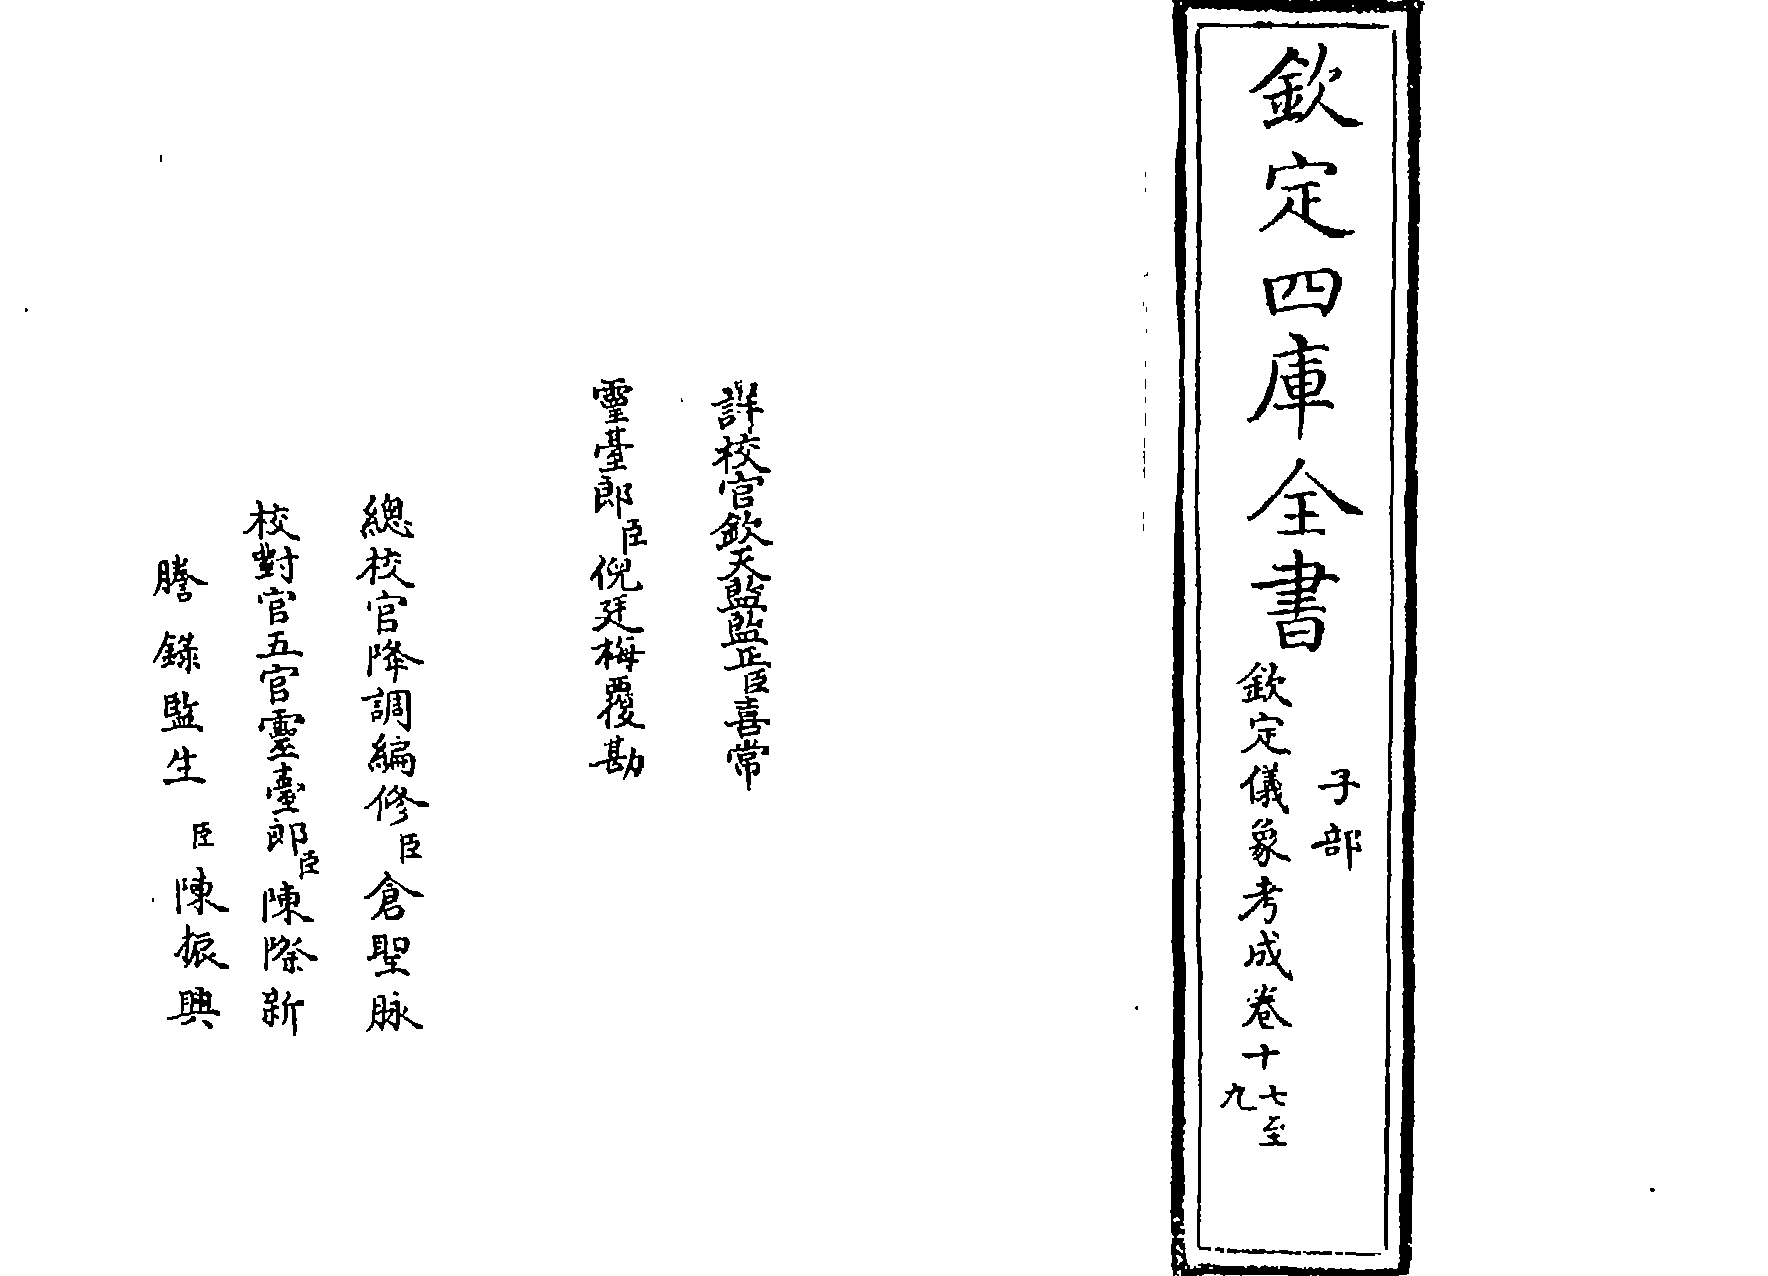
\includegraphics[width=\paperwidth,height=\paperheight,keepaspectratio]{img/1152.png}\clearpage
\begin{正文}
% ---- 册793 葉1153 ----
\SetPageNumber{1}
欽定四庫全書\换行
欽定儀象考成卷十七\换行
　恒星赤道經緯度表四\换行
　　赤道降婁宫\双列{\右小列{黄道度附}\左小列{}}\换行
\char"200B\relax\换行
\char"200B\relax\换行
\char"200B\relax\换行
\char"200B\relax\换行
\char"200B\relax\换行
\char"200B\relax\换行
\char"200B\relax\换行
\char"200B\relax\换行
\char"200B\relax\换行
\char"200B\relax\换行
\char"200B\relax\换行
\char"200B\relax
\par
\end{正文}\clearpage
\嵌图{146.67pt}{202.46pt}{838.42pt}{584.87pt}{img/1156.png}
\begin{正文}
% ---- 册793 葉1156 图版 ----
\SetPageNumber{2}
\插图页
\char"200B\relax\换行
\char"200B\relax\换行
\char"200B\relax\换行
\char"200B\relax\换行
\char"200B\relax\换行
\char"200B\relax\换行
\char"200B\relax\换行
\char"200B\relax\换行
\char"200B\relax\换行
\char"200B\relax\换行
\char"200B\relax\换行
\char"200B\relax\换行
\char"200B\relax\换行
\char"200B\relax\换行
\char"200B\relax\换行
\char"200B\relax
\恢复丝栏\par
\end{正文}\clearpage
\嵌图{148.67pt}{202.87pt}{834.42pt}{584.06pt}{img/1157.png}
\begin{正文}
% ---- 册793 葉1157 图版 ----
\SetPageNumber{3}
\插图页
\char"200B\relax\换行
\char"200B\relax\换行
\char"200B\relax\换行
\char"200B\relax\换行
\char"200B\relax\换行
\char"200B\relax\换行
\char"200B\relax\换行
\char"200B\relax\换行
\char"200B\relax\换行
\char"200B\relax\换行
\char"200B\relax\换行
\char"200B\relax\换行
\char"200B\relax\换行
\char"200B\relax\换行
\char"200B\relax\换行
\char"200B\relax
\恢复丝栏\par
\end{正文}\clearpage
\嵌图{142.64pt}{201.97pt}{846.47pt}{585.85pt}{img/1160.png}
\begin{正文}
% ---- 册793 葉1160 图版 ----
\SetPageNumber{4}
\插图页
\char"200B\relax\换行
\char"200B\relax\换行
\char"200B\relax\换行
\char"200B\relax\换行
\char"200B\relax\换行
\char"200B\relax\换行
\char"200B\relax\换行
\char"200B\relax\换行
\char"200B\relax\换行
\char"200B\relax\换行
\char"200B\relax\换行
\char"200B\relax\换行
\char"200B\relax\换行
\char"200B\relax\换行
\char"200B\relax\换行
\char"200B\relax
\恢复丝栏\par
\end{正文}\clearpage
\嵌图{146.62pt}{202.89pt}{838.53pt}{584.00pt}{img/1161.png}
\begin{正文}
% ---- 册793 葉1161 图版 ----
\SetPageNumber{5}
\插图页
\char"200B\relax\换行
\char"200B\relax\换行
\char"200B\relax\换行
\char"200B\relax\换行
\char"200B\relax\换行
\char"200B\relax\换行
\char"200B\relax\换行
\char"200B\relax\换行
\char"200B\relax\换行
\char"200B\relax\换行
\char"200B\relax\换行
\char"200B\relax\换行
\char"200B\relax\换行
\char"200B\relax\换行
\char"200B\relax\换行
\char"200B\relax
\恢复丝栏\par
\end{正文}\clearpage
\嵌图{144.63pt}{201.02pt}{842.50pt}{587.76pt}{img/1164.png}
\begin{正文}
% ---- 册793 葉1164 图版 ----
\SetPageNumber{6}
\插图页
\char"200B\relax\换行
\char"200B\relax\换行
\char"200B\relax\换行
\char"200B\relax\换行
\char"200B\relax\换行
\char"200B\relax\换行
\char"200B\relax\换行
\char"200B\relax\换行
\char"200B\relax\换行
\char"200B\relax\换行
\char"200B\relax\换行
\char"200B\relax\换行
\char"200B\relax\换行
\char"200B\relax\换行
\char"200B\relax\换行
\char"200B\relax
\恢复丝栏\par
\end{正文}\clearpage
\嵌图{146.62pt}{203.80pt}{838.53pt}{582.19pt}{img/1165.png}
\begin{正文}
% ---- 册793 葉1165 图版 ----
\SetPageNumber{7}
\插图页
\char"200B\relax\换行
\char"200B\relax\换行
\char"200B\relax\换行
\char"200B\relax\换行
\char"200B\relax\换行
\char"200B\relax\换行
\char"200B\relax\换行
\char"200B\relax\换行
\char"200B\relax\换行
\char"200B\relax\换行
\char"200B\relax\换行
\char"200B\relax\换行
\char"200B\relax\换行
\char"200B\relax\换行
\char"200B\relax\换行
\char"200B\relax
\恢复丝栏\par
\end{正文}\clearpage
\嵌图{140.71pt}{205.34pt}{850.34pt}{579.11pt}{img/1168.png}
\begin{正文}
% ---- 册793 葉1168 图版 ----
\SetPageNumber{8}
\插图页
\char"200B\relax\换行
\char"200B\relax\换行
\char"200B\relax\换行
\char"200B\relax\换行
\char"200B\relax\换行
\char"200B\relax\换行
\char"200B\relax\换行
\char"200B\relax\换行
\char"200B\relax\换行
\char"200B\relax\换行
\char"200B\relax\换行
\char"200B\relax\换行
\char"200B\relax\换行
\char"200B\relax\换行
\char"200B\relax\换行
\char"200B\relax
\恢复丝栏\par
\end{正文}\clearpage
\嵌图{142.72pt}{202.02pt}{846.33pt}{585.75pt}{img/1169.png}
\begin{正文}
% ---- 册793 葉1169 图版 ----
\SetPageNumber{9}
\插图页
\char"200B\relax\换行
\char"200B\relax\换行
\char"200B\relax\换行
\char"200B\relax\换行
\char"200B\relax\换行
\char"200B\relax\换行
\char"200B\relax\换行
\char"200B\relax\换行
\char"200B\relax\换行
\char"200B\relax\换行
\char"200B\relax\换行
\char"200B\relax\换行
\char"200B\relax\换行
\char"200B\relax\换行
\char"200B\relax\换行
\char"200B\relax
\恢复丝栏\par
\end{正文}\clearpage
\嵌图{144.63pt}{204.80pt}{842.50pt}{580.18pt}{img/1172.png}
\begin{正文}
% ---- 册793 葉1172 图版 ----
\SetPageNumber{10}
\插图页
\char"200B\relax\换行
\char"200B\relax\换行
\char"200B\relax\换行
\char"200B\relax\换行
\char"200B\relax\换行
\char"200B\relax\换行
\char"200B\relax\换行
\char"200B\relax\换行
\char"200B\relax\换行
\char"200B\relax\换行
\char"200B\relax\换行
\char"200B\relax\换行
\char"200B\relax\换行
\char"200B\relax\换行
\char"200B\relax\换行
\char"200B\relax
\恢复丝栏\par
\end{正文}\clearpage
\嵌图{146.62pt}{203.78pt}{838.53pt}{582.23pt}{img/1173.png}
\begin{正文}
% ---- 册793 葉1173 图版 ----
\SetPageNumber{11}
\插图页
\char"200B\relax\换行
\char"200B\relax\换行
\char"200B\relax\换行
\char"200B\relax\换行
\char"200B\relax\换行
\char"200B\relax\换行
\char"200B\relax\换行
\char"200B\relax\换行
\char"200B\relax\换行
\char"200B\relax\换行
\char"200B\relax\换行
\char"200B\relax\换行
\char"200B\relax\换行
\char"200B\relax\换行
\char"200B\relax\换行
\char"200B\relax
\恢复丝栏\par
\end{正文}\clearpage
\嵌图{140.68pt}{203.00pt}{850.39pt}{583.79pt}{img/1176.png}
\begin{正文}
% ---- 册793 葉1176 图版 ----
\SetPageNumber{12}
\插图页
\char"200B\relax\换行
\char"200B\relax\换行
\char"200B\relax\换行
\char"200B\relax\换行
\char"200B\relax\换行
\char"200B\relax\换行
\char"200B\relax\换行
\char"200B\relax\换行
\char"200B\relax\换行
\char"200B\relax\换行
\char"200B\relax\换行
\char"200B\relax\换行
\char"200B\relax\换行
\char"200B\relax\换行
\char"200B\relax\换行
\char"200B\relax
\恢复丝栏\par
\end{正文}\clearpage
\嵌图{142.68pt}{202.50pt}{846.40pt}{584.78pt}{img/1177.png}
\begin{正文}
% ---- 册793 葉1177 图版 ----
\SetPageNumber{13}
\插图页
\char"200B\relax\换行
\char"200B\relax\换行
\char"200B\relax\换行
\char"200B\relax\换行
\char"200B\relax\换行
\char"200B\relax\换行
\char"200B\relax\换行
\char"200B\relax\换行
\char"200B\relax\换行
\char"200B\relax\换行
\char"200B\relax\换行
\char"200B\relax\换行
\char"200B\relax\换行
\char"200B\relax\换行
\char"200B\relax\换行
\char"200B\relax
\恢复丝栏\par
\end{正文}\clearpage
\嵌图{144.68pt}{203.81pt}{842.41pt}{582.17pt}{img/1180.png}
\begin{正文}
% ---- 册793 葉1180 图版 ----
\SetPageNumber{14}
\插图页
\char"200B\relax\换行
\char"200B\relax\换行
\char"200B\relax\换行
\char"200B\relax\换行
\char"200B\relax\换行
\char"200B\relax\换行
\char"200B\relax\换行
\char"200B\relax\换行
\char"200B\relax\换行
\char"200B\relax\换行
\char"200B\relax\换行
\char"200B\relax\换行
\char"200B\relax\换行
\char"200B\relax\换行
\char"200B\relax\换行
\char"200B\relax
\恢复丝栏\par
\end{正文}\clearpage
\嵌图{144.68pt}{202.45pt}{842.41pt}{584.88pt}{img/1181.png}
\begin{正文}
% ---- 册793 葉1181 图版 ----
\SetPageNumber{15}
\插图页
\char"200B\relax\换行
\char"200B\relax\换行
\char"200B\relax\换行
\char"200B\relax\换行
\char"200B\relax\换行
\char"200B\relax\换行
\char"200B\relax\换行
\char"200B\relax\换行
\char"200B\relax\换行
\char"200B\relax\换行
\char"200B\relax\换行
\char"200B\relax\换行
\char"200B\relax\换行
\char"200B\relax\换行
\char"200B\relax\换行
\char"200B\relax
\恢复丝栏\par
\end{正文}\clearpage
\嵌图{140.66pt}{201.50pt}{850.45pt}{586.80pt}{img/1184.png}
\begin{正文}
% ---- 册793 葉1184 图版 ----
\SetPageNumber{16}
\插图页
\char"200B\relax\换行
\char"200B\relax\换行
\char"200B\relax\换行
\char"200B\relax\换行
\char"200B\relax\换行
\char"200B\relax\换行
\char"200B\relax\换行
\char"200B\relax\换行
\char"200B\relax\换行
\char"200B\relax\换行
\char"200B\relax\换行
\char"200B\relax\换行
\char"200B\relax\换行
\char"200B\relax\换行
\char"200B\relax\换行
\char"200B\relax
\恢复丝栏\par
\end{正文}\clearpage
\嵌图{142.64pt}{201.51pt}{846.47pt}{586.77pt}{img/1185.png}
\begin{正文}
% ---- 册793 葉1185 图版 ----
\SetPageNumber{17}
\插图页
\char"200B\relax\换行
\char"200B\relax\换行
\char"200B\relax\换行
\char"200B\relax\换行
\char"200B\relax\换行
\char"200B\relax\换行
\char"200B\relax\换行
\char"200B\relax\换行
\char"200B\relax\换行
\char"200B\relax\换行
\char"200B\relax\换行
\char"200B\relax\换行
\char"200B\relax\换行
\char"200B\relax\换行
\char"200B\relax\换行
\char"200B\relax
\恢复丝栏\par
\end{正文}\clearpage
\嵌图{146.67pt}{201.02pt}{838.42pt}{587.74pt}{img/1188.png}
\begin{正文}
% ---- 册793 葉1188 图版 ----
\SetPageNumber{18}
\插图页
\char"200B\relax\换行
\char"200B\relax\换行
\char"200B\relax\换行
\char"200B\relax\换行
\char"200B\relax\换行
\char"200B\relax\换行
\char"200B\relax\换行
\char"200B\relax\换行
\char"200B\relax\换行
\char"200B\relax\换行
\char"200B\relax\换行
\char"200B\relax\换行
\char"200B\relax\换行
\char"200B\relax\换行
\char"200B\relax\换行
\char"200B\relax
\恢复丝栏\par
\end{正文}\clearpage
\嵌图{146.67pt}{202.92pt}{838.42pt}{583.95pt}{img/1189.png}
\begin{正文}
% ---- 册793 葉1189 图版 ----
\SetPageNumber{19}
\插图页
\char"200B\relax\换行
\char"200B\relax\换行
\char"200B\relax\换行
\char"200B\relax\换行
\char"200B\relax\换行
\char"200B\relax\换行
\char"200B\relax\换行
\char"200B\relax\换行
\char"200B\relax\换行
\char"200B\relax\换行
\char"200B\relax\换行
\char"200B\relax\换行
\char"200B\relax\换行
\char"200B\relax\换行
\char"200B\relax\换行
\char"200B\relax
\恢复丝栏\par
\end{正文}\clearpage
\嵌图{150.30pt}{206.70pt}{831.15pt}{576.39pt}{img/1192.png}
\begin{正文}
% ---- 册793 葉1192 图版 ----
\SetPageNumber{20}
\插图页
\char"200B\relax\换行
\char"200B\relax\换行
\char"200B\relax\换行
\char"200B\relax\换行
\char"200B\relax\换行
\char"200B\relax\换行
\char"200B\relax\换行
\char"200B\relax\换行
\char"200B\relax\换行
\char"200B\relax\换行
\char"200B\relax\换行
\char"200B\relax\换行
\char"200B\relax\换行
\char"200B\relax\换行
\char"200B\relax\换行
\char"200B\relax
\恢复丝栏\par
\end{正文}\clearpage
\嵌图{193.20pt}{210.32pt}{543.58pt}{582.51pt}{img/1193.png}
\begin{正文}
% ---- 册793 葉1193 ----
\SetPageNumber{21}
\插图页
\char"200B\relax\换行
\char"200B\relax\换行
\char"200B\relax\换行
\char"200B\relax\换行
\char"200B\relax\换行
\char"200B\relax\换行
\char"200B\relax\换行
\char"200B\relax\换行
\恢复丝栏
\char"200B\relax\换行
\char"200B\relax\换行
\char"200B\relax\换行
\char"200B\relax\换行
\char"200B\relax\换行
\char"200B\relax\换行
\char"200B\relax\换行
欽定儀象考成卷十七
\par

% ======== 卷十八（8行21字）========
\par\end{正文}\clearpage
\chapter*{欽定儀象考成卷十八}
\begin{正文}
% ---- 册793 葉1196 ----
\SetPageNumber{1}
欽定四庫全書\换行
欽定儀象考成卷十八\换行
　恒星赤道經緯度表五\换行
　　赤道大梁宫\双列{\右小列{黄道度附}\左小列{}}\换行
\char"200B\relax\换行
\char"200B\relax\换行
\char"200B\relax\换行
\char"200B\relax\换行
\char"200B\relax\换行
\char"200B\relax\换行
\char"200B\relax\换行
\char"200B\relax\换行
\char"200B\relax\换行
\char"200B\relax\换行
\char"200B\relax\换行
\char"200B\relax
\par
\end{正文}\clearpage
\嵌图{144.63pt}{202.85pt}{842.50pt}{584.09pt}{img/1197.png}
\begin{正文}
% ---- 册793 葉1197 图版 ----
\SetPageNumber{2}
\插图页
\char"200B\relax\换行
\char"200B\relax\换行
\char"200B\relax\换行
\char"200B\relax\换行
\char"200B\relax\换行
\char"200B\relax\换行
\char"200B\relax\换行
\char"200B\relax\换行
\char"200B\relax\换行
\char"200B\relax\换行
\char"200B\relax\换行
\char"200B\relax\换行
\char"200B\relax\换行
\char"200B\relax\换行
\char"200B\relax\换行
\char"200B\relax
\恢复丝栏\par
\end{正文}\clearpage
\嵌图{142.68pt}{201.56pt}{846.40pt}{586.67pt}{img/1200.png}
\begin{正文}
% ---- 册793 葉1200 图版 ----
\SetPageNumber{3}
\插图页
\char"200B\relax\换行
\char"200B\relax\换行
\char"200B\relax\换行
\char"200B\relax\换行
\char"200B\relax\换行
\char"200B\relax\换行
\char"200B\relax\换行
\char"200B\relax\换行
\char"200B\relax\换行
\char"200B\relax\换行
\char"200B\relax\换行
\char"200B\relax\换行
\char"200B\relax\换行
\char"200B\relax\换行
\char"200B\relax\换行
\char"200B\relax
\恢复丝栏\par
\end{正文}\clearpage
\嵌图{142.68pt}{202.49pt}{846.40pt}{584.80pt}{img/1201.png}
\begin{正文}
% ---- 册793 葉1201 图版 ----
\SetPageNumber{4}
\插图页
\char"200B\relax\换行
\char"200B\relax\换行
\char"200B\relax\换行
\char"200B\relax\换行
\char"200B\relax\换行
\char"200B\relax\换行
\char"200B\relax\换行
\char"200B\relax\换行
\char"200B\relax\换行
\char"200B\relax\换行
\char"200B\relax\换行
\char"200B\relax\换行
\char"200B\relax\换行
\char"200B\relax\换行
\char"200B\relax\换行
\char"200B\relax
\恢复丝栏\par
\end{正文}\clearpage
\嵌图{146.62pt}{201.48pt}{838.53pt}{586.83pt}{img/1204.png}
\begin{正文}
% ---- 册793 葉1204 图版 ----
\SetPageNumber{5}
\插图页
\char"200B\relax\换行
\char"200B\relax\换行
\char"200B\relax\换行
\char"200B\relax\换行
\char"200B\relax\换行
\char"200B\relax\换行
\char"200B\relax\换行
\char"200B\relax\换行
\char"200B\relax\换行
\char"200B\relax\换行
\char"200B\relax\换行
\char"200B\relax\换行
\char"200B\relax\换行
\char"200B\relax\换行
\char"200B\relax\换行
\char"200B\relax
\恢复丝栏\par
\end{正文}\clearpage
\嵌图{146.62pt}{201.01pt}{838.53pt}{587.77pt}{img/1205.png}
\begin{正文}
% ---- 册793 葉1205 图版 ----
\SetPageNumber{6}
\插图页
\char"200B\relax\换行
\char"200B\relax\换行
\char"200B\relax\换行
\char"200B\relax\换行
\char"200B\relax\换行
\char"200B\relax\换行
\char"200B\relax\换行
\char"200B\relax\换行
\char"200B\relax\换行
\char"200B\relax\换行
\char"200B\relax\换行
\char"200B\relax\换行
\char"200B\relax\换行
\char"200B\relax\换行
\char"200B\relax\换行
\char"200B\relax
\恢复丝栏\par
\end{正文}\clearpage
\嵌图{144.68pt}{201.57pt}{842.41pt}{586.66pt}{img/1208.png}
\begin{正文}
% ---- 册793 葉1208 图版 ----
\SetPageNumber{7}
\插图页
\char"200B\relax\换行
\char"200B\relax\换行
\char"200B\relax\换行
\char"200B\relax\换行
\char"200B\relax\换行
\char"200B\relax\换行
\char"200B\relax\换行
\char"200B\relax\换行
\char"200B\relax\换行
\char"200B\relax\换行
\char"200B\relax\换行
\char"200B\relax\换行
\char"200B\relax\换行
\char"200B\relax\换行
\char"200B\relax\换行
\char"200B\relax
\恢复丝栏\par
\end{正文}\clearpage
\嵌图{142.68pt}{202.52pt}{846.40pt}{584.75pt}{img/1209.png}
\begin{正文}
% ---- 册793 葉1209 图版 ----
\SetPageNumber{8}
\插图页
\char"200B\relax\换行
\char"200B\relax\换行
\char"200B\relax\换行
\char"200B\relax\换行
\char"200B\relax\换行
\char"200B\relax\换行
\char"200B\relax\换行
\char"200B\relax\换行
\char"200B\relax\换行
\char"200B\relax\换行
\char"200B\relax\换行
\char"200B\relax\换行
\char"200B\relax\换行
\char"200B\relax\换行
\char"200B\relax\换行
\char"200B\relax
\恢复丝栏\par
\end{正文}\clearpage
\嵌图{146.67pt}{200.53pt}{838.42pt}{588.73pt}{img/1212.png}
\begin{正文}
% ---- 册793 葉1212 图版 ----
\SetPageNumber{9}
\插图页
\char"200B\relax\换行
\char"200B\relax\换行
\char"200B\relax\换行
\char"200B\relax\换行
\char"200B\relax\换行
\char"200B\relax\换行
\char"200B\relax\换行
\char"200B\relax\换行
\char"200B\relax\换行
\char"200B\relax\换行
\char"200B\relax\换行
\char"200B\relax\换行
\char"200B\relax\换行
\char"200B\relax\换行
\char"200B\relax\换行
\char"200B\relax
\恢复丝栏\par
\end{正文}\clearpage
\嵌图{146.67pt}{201.03pt}{838.42pt}{587.73pt}{img/1213.png}
\begin{正文}
% ---- 册793 葉1213 图版 ----
\SetPageNumber{10}
\插图页
\char"200B\relax\换行
\char"200B\relax\换行
\char"200B\relax\换行
\char"200B\relax\换行
\char"200B\relax\换行
\char"200B\relax\换行
\char"200B\relax\换行
\char"200B\relax\换行
\char"200B\relax\换行
\char"200B\relax\换行
\char"200B\relax\换行
\char"200B\relax\换行
\char"200B\relax\换行
\char"200B\relax\换行
\char"200B\relax\换行
\char"200B\relax
\恢复丝栏\par
\end{正文}\clearpage
\嵌图{148.61pt}{200.57pt}{834.55pt}{588.65pt}{img/1216.png}
\begin{正文}
% ---- 册793 葉1216 图版 ----
\SetPageNumber{11}
\插图页
\char"200B\relax\换行
\char"200B\relax\换行
\char"200B\relax\换行
\char"200B\relax\换行
\char"200B\relax\换行
\char"200B\relax\换行
\char"200B\relax\换行
\char"200B\relax\换行
\char"200B\relax\换行
\char"200B\relax\换行
\char"200B\relax\换行
\char"200B\relax\换行
\char"200B\relax\换行
\char"200B\relax\换行
\char"200B\relax\换行
\char"200B\relax
\恢复丝栏\par
\end{正文}\clearpage
\嵌图{144.63pt}{202.01pt}{842.50pt}{585.77pt}{img/1217.png}
\begin{正文}
% ---- 册793 葉1217 图版 ----
\SetPageNumber{12}
\插图页
\char"200B\relax\换行
\char"200B\relax\换行
\char"200B\relax\换行
\char"200B\relax\换行
\char"200B\relax\换行
\char"200B\relax\换行
\char"200B\relax\换行
\char"200B\relax\换行
\char"200B\relax\换行
\char"200B\relax\换行
\char"200B\relax\换行
\char"200B\relax\换行
\char"200B\relax\换行
\char"200B\relax\换行
\char"200B\relax\换行
\char"200B\relax
\恢复丝栏\par
\end{正文}\clearpage
\嵌图{146.62pt}{200.59pt}{838.53pt}{588.61pt}{img/1220.png}
\begin{正文}
% ---- 册793 葉1220 图版 ----
\SetPageNumber{13}
\插图页
\char"200B\relax\换行
\char"200B\relax\换行
\char"200B\relax\换行
\char"200B\relax\换行
\char"200B\relax\换行
\char"200B\relax\换行
\char"200B\relax\换行
\char"200B\relax\换行
\char"200B\relax\换行
\char"200B\relax\换行
\char"200B\relax\换行
\char"200B\relax\换行
\char"200B\relax\换行
\char"200B\relax\换行
\char"200B\relax\换行
\char"200B\relax
\恢复丝栏\par
\end{正文}\clearpage
\嵌图{144.63pt}{201.02pt}{842.50pt}{587.76pt}{img/1221.png}
\begin{正文}
% ---- 册793 葉1221 图版 ----
\SetPageNumber{14}
\插图页
\char"200B\relax\换行
\char"200B\relax\换行
\char"200B\relax\换行
\char"200B\relax\换行
\char"200B\relax\换行
\char"200B\relax\换行
\char"200B\relax\换行
\char"200B\relax\换行
\char"200B\relax\换行
\char"200B\relax\换行
\char"200B\relax\换行
\char"200B\relax\换行
\char"200B\relax\换行
\char"200B\relax\换行
\char"200B\relax\换行
\char"200B\relax
\恢复丝栏\par
\end{正文}\clearpage
\嵌图{146.56pt}{202.00pt}{838.64pt}{585.78pt}{img/1224.png}
\begin{正文}
% ---- 册793 葉1224 图版 ----
\SetPageNumber{15}
\插图页
\char"200B\relax\换行
\char"200B\relax\换行
\char"200B\relax\换行
\char"200B\relax\换行
\char"200B\relax\换行
\char"200B\relax\换行
\char"200B\relax\换行
\char"200B\relax\换行
\char"200B\relax\换行
\char"200B\relax\换行
\char"200B\relax\换行
\char"200B\relax\换行
\char"200B\relax\换行
\char"200B\relax\换行
\char"200B\relax\换行
\char"200B\relax
\恢复丝栏\par
\end{正文}\clearpage
\嵌图{148.54pt}{200.55pt}{834.68pt}{588.69pt}{img/1225.png}
\begin{正文}
% ---- 册793 葉1225 图版 ----
\SetPageNumber{16}
\插图页
\char"200B\relax\换行
\char"200B\relax\换行
\char"200B\relax\换行
\char"200B\relax\换行
\char"200B\relax\换行
\char"200B\relax\换行
\char"200B\relax\换行
\char"200B\relax\换行
\char"200B\relax\换行
\char"200B\relax\换行
\char"200B\relax\换行
\char"200B\relax\换行
\char"200B\relax\换行
\char"200B\relax\换行
\char"200B\relax\换行
\char"200B\relax
\恢复丝栏\par
\end{正文}\clearpage
\嵌图{146.56pt}{202.93pt}{838.64pt}{583.94pt}{img/1228.png}
\begin{正文}
% ---- 册793 葉1228 图版 ----
\SetPageNumber{17}
\插图页
\char"200B\relax\换行
\char"200B\relax\换行
\char"200B\relax\换行
\char"200B\relax\换行
\char"200B\relax\换行
\char"200B\relax\换行
\char"200B\relax\换行
\char"200B\relax\换行
\char"200B\relax\换行
\char"200B\relax\换行
\char"200B\relax\换行
\char"200B\relax\换行
\char"200B\relax\换行
\char"200B\relax\换行
\char"200B\relax\换行
\char"200B\relax
\恢复丝栏\par
\end{正文}\clearpage
\嵌图{148.54pt}{200.49pt}{834.68pt}{588.80pt}{img/1229.png}
\begin{正文}
% ---- 册793 葉1229 图版 ----
\SetPageNumber{18}
\插图页
\char"200B\relax\换行
\char"200B\relax\换行
\char"200B\relax\换行
\char"200B\relax\换行
\char"200B\relax\换行
\char"200B\relax\换行
\char"200B\relax\换行
\char"200B\relax\换行
\char"200B\relax\换行
\char"200B\relax\换行
\char"200B\relax\换行
\char"200B\relax\换行
\char"200B\relax\换行
\char"200B\relax\换行
\char"200B\relax\换行
\char"200B\relax
\恢复丝栏\par
\end{正文}\clearpage
\嵌图{154.21pt}{201.07pt}{823.35pt}{587.64pt}{img/1232.png}
\begin{正文}
% ---- 册793 葉1232 图版 ----
\SetPageNumber{19}
\插图页
\char"200B\relax\换行
\char"200B\relax\换行
\char"200B\relax\换行
\char"200B\relax\换行
\char"200B\relax\换行
\char"200B\relax\换行
\char"200B\relax\换行
\char"200B\relax\换行
\char"200B\relax\换行
\char"200B\relax\换行
\char"200B\relax\换行
\char"200B\relax\换行
\char"200B\relax\换行
\char"200B\relax\换行
\char"200B\relax\换行
\char"200B\relax
\恢复丝栏\par
\end{正文}\clearpage
\嵌图{170.46pt}{235.03pt}{173.48pt}{586.18pt}{img/1233.png}
\begin{正文}
% ---- 册793 葉1233 ----
\SetPageNumber{20}
\char"200B\relax\换行
\char"200B\relax\换行
\char"200B\relax\换行
\char"200B\relax\换行
\char"200B\relax\换行
\char"200B\relax\换行
\char"200B\relax\换行
\char"200B\relax\换行
\char"200B\relax\换行
\char"200B\relax\换行
\char"200B\relax\换行
\char"200B\relax\换行
\char"200B\relax\换行
\char"200B\relax\换行
\char"200B\relax\换行
欽定儀象考成卷十八
\par

% ======== 卷十九（8行21字）========
\par\end{正文}\clearpage
\chapter*{欽定儀象考成卷十九}
\begin{正文}
% ---- 册793 葉1236 ----
\SetPageNumber{1}
欽定四庫全書\换行
欽定儀象考成卷十九\换行
　恒星赤道經緯度表六\换行
　　赤道實沈宫\双列{\右小列{黄道度附}\左小列{}}\换行
\char"200B\relax\换行
\char"200B\relax\换行
\char"200B\relax\换行
\char"200B\relax\换行
\char"200B\relax\换行
\char"200B\relax\换行
\char"200B\relax\换行
\char"200B\relax\换行
\char"200B\relax\换行
\char"200B\relax\换行
\char"200B\relax\换行
\char"200B\relax
\par
\end{正文}\clearpage
\嵌图{146.56pt}{200.07pt}{838.64pt}{589.65pt}{img/1237.png}
\begin{正文}
% ---- 册793 葉1237 图版 ----
\SetPageNumber{2}
\插图页
\char"200B\relax\换行
\char"200B\relax\换行
\char"200B\relax\换行
\char"200B\relax\换行
\char"200B\relax\换行
\char"200B\relax\换行
\char"200B\relax\换行
\char"200B\relax\换行
\char"200B\relax\换行
\char"200B\relax\换行
\char"200B\relax\换行
\char"200B\relax\换行
\char"200B\relax\换行
\char"200B\relax\换行
\char"200B\relax\换行
\char"200B\relax
\恢复丝栏\par
\end{正文}\clearpage
\嵌图{144.63pt}{202.03pt}{842.50pt}{585.74pt}{img/1240.png}
\begin{正文}
% ---- 册793 葉1240 图版 ----
\SetPageNumber{3}
\插图页
\char"200B\relax\换行
\char"200B\relax\换行
\char"200B\relax\换行
\char"200B\relax\换行
\char"200B\relax\换行
\char"200B\relax\换行
\char"200B\relax\换行
\char"200B\relax\换行
\char"200B\relax\换行
\char"200B\relax\换行
\char"200B\relax\换行
\char"200B\relax\换行
\char"200B\relax\换行
\char"200B\relax\换行
\char"200B\relax\换行
\char"200B\relax
\恢复丝栏\par
\end{正文}\clearpage
\嵌图{144.63pt}{200.59pt}{842.50pt}{588.61pt}{img/1241.png}
\begin{正文}
% ---- 册793 葉1241 图版 ----
\SetPageNumber{4}
\插图页
\char"200B\relax\换行
\char"200B\relax\换行
\char"200B\relax\换行
\char"200B\relax\换行
\char"200B\relax\换行
\char"200B\relax\换行
\char"200B\relax\换行
\char"200B\relax\换行
\char"200B\relax\换行
\char"200B\relax\换行
\char"200B\relax\换行
\char"200B\relax\换行
\char"200B\relax\换行
\char"200B\relax\换行
\char"200B\relax\换行
\char"200B\relax
\恢复丝栏\par
\end{正文}\clearpage
\嵌图{144.68pt}{201.56pt}{842.41pt}{586.67pt}{img/1244.png}
\begin{正文}
% ---- 册793 葉1244 图版 ----
\SetPageNumber{5}
\插图页
\char"200B\relax\换行
\char"200B\relax\换行
\char"200B\relax\换行
\char"200B\relax\换行
\char"200B\relax\换行
\char"200B\relax\换行
\char"200B\relax\换行
\char"200B\relax\换行
\char"200B\relax\换行
\char"200B\relax\换行
\char"200B\relax\换行
\char"200B\relax\换行
\char"200B\relax\换行
\char"200B\relax\换行
\char"200B\relax\换行
\char"200B\relax
\恢复丝栏\par
\end{正文}\clearpage
\嵌图{142.68pt}{202.90pt}{846.40pt}{583.99pt}{img/1245.png}
\begin{正文}
% ---- 册793 葉1245 图版 ----
\SetPageNumber{6}
\插图页
\char"200B\relax\换行
\char"200B\relax\换行
\char"200B\relax\换行
\char"200B\relax\换行
\char"200B\relax\换行
\char"200B\relax\换行
\char"200B\relax\换行
\char"200B\relax\换行
\char"200B\relax\换行
\char"200B\relax\换行
\char"200B\relax\换行
\char"200B\relax\换行
\char"200B\relax\换行
\char"200B\relax\换行
\char"200B\relax\换行
\char"200B\relax
\恢复丝栏\par
\end{正文}\clearpage
\嵌图{142.64pt}{203.00pt}{846.47pt}{583.79pt}{img/1248.png}
\begin{正文}
% ---- 册793 葉1248 图版 ----
\SetPageNumber{7}
\插图页
\char"200B\relax\换行
\char"200B\relax\换行
\char"200B\relax\换行
\char"200B\relax\换行
\char"200B\relax\换行
\char"200B\relax\换行
\char"200B\relax\换行
\char"200B\relax\换行
\char"200B\relax\换行
\char"200B\relax\换行
\char"200B\relax\换行
\char"200B\relax\换行
\char"200B\relax\换行
\char"200B\relax\换行
\char"200B\relax\换行
\char"200B\relax
\恢复丝栏\par
\end{正文}\clearpage
\嵌图{146.62pt}{200.59pt}{838.53pt}{588.61pt}{img/1249.png}
\begin{正文}
% ---- 册793 葉1249 图版 ----
\SetPageNumber{8}
\插图页
\char"200B\relax\换行
\char"200B\relax\换行
\char"200B\relax\换行
\char"200B\relax\换行
\char"200B\relax\换行
\char"200B\relax\换行
\char"200B\relax\换行
\char"200B\relax\换行
\char"200B\relax\换行
\char"200B\relax\换行
\char"200B\relax\换行
\char"200B\relax\换行
\char"200B\relax\换行
\char"200B\relax\换行
\char"200B\relax\换行
\char"200B\relax
\恢复丝栏\par
\end{正文}\clearpage
\嵌图{146.62pt}{201.56pt}{838.53pt}{586.67pt}{img/1252.png}
\begin{正文}
% ---- 册793 葉1252 图版 ----
\SetPageNumber{9}
\插图页
\char"200B\relax\换行
\char"200B\relax\换行
\char"200B\relax\换行
\char"200B\relax\换行
\char"200B\relax\换行
\char"200B\relax\换行
\char"200B\relax\换行
\char"200B\relax\换行
\char"200B\relax\换行
\char"200B\relax\换行
\char"200B\relax\换行
\char"200B\relax\换行
\char"200B\relax\换行
\char"200B\relax\换行
\char"200B\relax\换行
\char"200B\relax
\恢复丝栏\par
\end{正文}\clearpage
\嵌图{144.63pt}{201.99pt}{842.50pt}{585.80pt}{img/1253.png}
\begin{正文}
% ---- 册793 葉1253 图版 ----
\SetPageNumber{10}
\插图页
\char"200B\relax\换行
\char"200B\relax\换行
\char"200B\relax\换行
\char"200B\relax\换行
\char"200B\relax\换行
\char"200B\relax\换行
\char"200B\relax\换行
\char"200B\relax\换行
\char"200B\relax\换行
\char"200B\relax\换行
\char"200B\relax\换行
\char"200B\relax\换行
\char"200B\relax\换行
\char"200B\relax\换行
\char"200B\relax\换行
\char"200B\relax
\恢复丝栏\par
\end{正文}\clearpage
\嵌图{144.59pt}{204.41pt}{842.59pt}{580.97pt}{img/1256.png}
\begin{正文}
% ---- 册793 葉1256 图版 ----
\SetPageNumber{11}
\插图页
\char"200B\relax\换行
\char"200B\relax\换行
\char"200B\relax\换行
\char"200B\relax\换行
\char"200B\relax\换行
\char"200B\relax\换行
\char"200B\relax\换行
\char"200B\relax\换行
\char"200B\relax\换行
\char"200B\relax\换行
\char"200B\relax\换行
\char"200B\relax\换行
\char"200B\relax\换行
\char"200B\relax\换行
\char"200B\relax\换行
\char"200B\relax
\恢复丝栏\par
\end{正文}\clearpage
\嵌图{142.61pt}{202.95pt}{846.55pt}{583.88pt}{img/1257.png}
\begin{正文}
% ---- 册793 葉1257 图版 ----
\SetPageNumber{12}
\插图页
\char"200B\relax\换行
\char"200B\relax\换行
\char"200B\relax\换行
\char"200B\relax\换行
\char"200B\relax\换行
\char"200B\relax\换行
\char"200B\relax\换行
\char"200B\relax\换行
\char"200B\relax\换行
\char"200B\relax\换行
\char"200B\relax\换行
\char"200B\relax\换行
\char"200B\relax\换行
\char"200B\relax\换行
\char"200B\relax\换行
\char"200B\relax
\恢复丝栏\par
\end{正文}\clearpage
\嵌图{146.62pt}{202.89pt}{838.53pt}{584.00pt}{img/1260.png}
\begin{正文}
% ---- 册793 葉1260 图版 ----
\SetPageNumber{13}
\插图页
\char"200B\relax\换行
\char"200B\relax\换行
\char"200B\relax\换行
\char"200B\relax\换行
\char"200B\relax\换行
\char"200B\relax\换行
\char"200B\relax\换行
\char"200B\relax\换行
\char"200B\relax\换行
\char"200B\relax\换行
\char"200B\relax\换行
\char"200B\relax\换行
\char"200B\relax\换行
\char"200B\relax\换行
\char"200B\relax\换行
\char"200B\relax
\恢复丝栏\par
\end{正文}\clearpage
\嵌图{142.64pt}{200.99pt}{846.47pt}{587.82pt}{img/1261.png}
\begin{正文}
% ---- 册793 葉1261 图版 ----
\SetPageNumber{14}
\插图页
\char"200B\relax\换行
\char"200B\relax\换行
\char"200B\relax\换行
\char"200B\relax\换行
\char"200B\relax\换行
\char"200B\relax\换行
\char"200B\relax\换行
\char"200B\relax\换行
\char"200B\relax\换行
\char"200B\relax\换行
\char"200B\relax\换行
\char"200B\relax\换行
\char"200B\relax\换行
\char"200B\relax\换行
\char"200B\relax\换行
\char"200B\relax
\恢复丝栏\par
\end{正文}\clearpage
\嵌图{144.63pt}{202.02pt}{842.50pt}{585.75pt}{img/1264.png}
\begin{正文}
% ---- 册793 葉1264 图版 ----
\SetPageNumber{15}
\插图页
\char"200B\relax\换行
\char"200B\relax\换行
\char"200B\relax\换行
\char"200B\relax\换行
\char"200B\relax\换行
\char"200B\relax\换行
\char"200B\relax\换行
\char"200B\relax\换行
\char"200B\relax\换行
\char"200B\relax\换行
\char"200B\relax\换行
\char"200B\relax\换行
\char"200B\relax\换行
\char"200B\relax\换行
\char"200B\relax\换行
\char"200B\relax
\恢复丝栏\par
\end{正文}\clearpage
\嵌图{142.64pt}{200.11pt}{846.47pt}{589.56pt}{img/1265.png}
\begin{正文}
% ---- 册793 葉1265 图版 ----
\SetPageNumber{16}
\插图页
\char"200B\relax\换行
\char"200B\relax\换行
\char"200B\relax\换行
\char"200B\relax\换行
\char"200B\relax\换行
\char"200B\relax\换行
\char"200B\relax\换行
\char"200B\relax\换行
\char"200B\relax\换行
\char"200B\relax\换行
\char"200B\relax\换行
\char"200B\relax\换行
\char"200B\relax\换行
\char"200B\relax\换行
\char"200B\relax\换行
\char"200B\relax
\恢复丝栏\par
\end{正文}\clearpage
\嵌图{144.59pt}{202.46pt}{842.59pt}{584.87pt}{img/1268.png}
\begin{正文}
% ---- 册793 葉1268 图版 ----
\SetPageNumber{17}
\插图页
\char"200B\relax\换行
\char"200B\relax\换行
\char"200B\relax\换行
\char"200B\relax\换行
\char"200B\relax\换行
\char"200B\relax\换行
\char"200B\relax\换行
\char"200B\relax\换行
\char"200B\relax\换行
\char"200B\relax\换行
\char"200B\relax\换行
\char"200B\relax\换行
\char"200B\relax\换行
\char"200B\relax\换行
\char"200B\relax\换行
\char"200B\relax
\恢复丝栏\par
\end{正文}\clearpage
\嵌图{144.59pt}{202.42pt}{842.59pt}{584.95pt}{img/1269.png}
\begin{正文}
% ---- 册793 葉1269 图版 ----
\SetPageNumber{18}
\插图页
\char"200B\relax\换行
\char"200B\relax\换行
\char"200B\relax\换行
\char"200B\relax\换行
\char"200B\relax\换行
\char"200B\relax\换行
\char"200B\relax\换行
\char"200B\relax\换行
\char"200B\relax\换行
\char"200B\relax\换行
\char"200B\relax\换行
\char"200B\relax\换行
\char"200B\relax\换行
\char"200B\relax\换行
\char"200B\relax\换行
\char"200B\relax
\恢复丝栏\par
\end{正文}\clearpage
\嵌图{148.61pt}{199.14pt}{834.55pt}{591.51pt}{img/1272.png}
\begin{正文}
% ---- 册793 葉1272 图版 ----
\SetPageNumber{19}
\插图页
\char"200B\relax\换行
\char"200B\relax\换行
\char"200B\relax\换行
\char"200B\relax\换行
\char"200B\relax\换行
\char"200B\relax\换行
\char"200B\relax\换行
\char"200B\relax\换行
\char"200B\relax\换行
\char"200B\relax\换行
\char"200B\relax\换行
\char"200B\relax\换行
\char"200B\relax\换行
\char"200B\relax\换行
\char"200B\relax\换行
\char"200B\relax
\恢复丝栏\par
\end{正文}\clearpage
\嵌图{146.62pt}{199.59pt}{838.53pt}{590.60pt}{img/1273.png}
\begin{正文}
% ---- 册793 葉1273 图版 ----
\SetPageNumber{20}
\插图页
\char"200B\relax\换行
\char"200B\relax\换行
\char"200B\relax\换行
\char"200B\relax\换行
\char"200B\relax\换行
\char"200B\relax\换行
\char"200B\relax\换行
\char"200B\relax\换行
\char"200B\relax\换行
\char"200B\relax\换行
\char"200B\relax\换行
\char"200B\relax\换行
\char"200B\relax\换行
\char"200B\relax\换行
\char"200B\relax\换行
\char"200B\relax
\恢复丝栏\par
\end{正文}\clearpage
\嵌图{144.68pt}{202.50pt}{842.41pt}{584.78pt}{img/1276.png}
\begin{正文}
% ---- 册793 葉1276 图版 ----
\SetPageNumber{21}
\插图页
\char"200B\relax\换行
\char"200B\relax\换行
\char"200B\relax\换行
\char"200B\relax\换行
\char"200B\relax\换行
\char"200B\relax\换行
\char"200B\relax\换行
\char"200B\relax\换行
\char"200B\relax\换行
\char"200B\relax\换行
\char"200B\relax\换行
\char"200B\relax\换行
\char"200B\relax\换行
\char"200B\relax\换行
\char"200B\relax\换行
\char"200B\relax
\恢复丝栏\par
\end{正文}\clearpage
\嵌图{146.67pt}{201.04pt}{838.42pt}{587.72pt}{img/1277.png}
\begin{正文}
% ---- 册793 葉1277 图版 ----
\SetPageNumber{22}
\插图页
\char"200B\relax\换行
\char"200B\relax\换行
\char"200B\relax\换行
\char"200B\relax\换行
\char"200B\relax\换行
\char"200B\relax\换行
\char"200B\relax\换行
\char"200B\relax\换行
\char"200B\relax\换行
\char"200B\relax\换行
\char"200B\relax\换行
\char"200B\relax\换行
\char"200B\relax\换行
\char"200B\relax\换行
\char"200B\relax\换行
\char"200B\relax
\恢复丝栏\par
\end{正文}\clearpage
\嵌图{148.42pt}{200.55pt}{834.93pt}{588.69pt}{img/1280.png}
\begin{正文}
% ---- 册793 葉1280 图版 ----
\SetPageNumber{23}
\插图页
\char"200B\relax\换行
\char"200B\relax\换行
\char"200B\relax\换行
\char"200B\relax\换行
\char"200B\relax\换行
\char"200B\relax\换行
\char"200B\relax\换行
\char"200B\relax\换行
\char"200B\relax\换行
\char"200B\relax\换行
\char"200B\relax\换行
\char"200B\relax\换行
\char"200B\relax\换行
\char"200B\relax\换行
\char"200B\relax\换行
\char"200B\relax
\恢复丝栏\par
\end{正文}\clearpage
\嵌图{141.38pt}{220.50pt}{406.64pt}{572.33pt}{img/1281.png}
\begin{正文}
% ---- 册793 葉1281 ----
\SetPageNumber{24}
\插图页
\char"200B\relax\换行
\char"200B\relax\换行
\char"200B\relax\换行
\char"200B\relax\换行
\char"200B\relax\换行
\char"200B\relax\换行
\char"200B\relax\换行
\char"200B\relax\换行
\恢复丝栏
\char"200B\relax\换行
\char"200B\relax\换行
\char"200B\relax\换行
\char"200B\relax\换行
\char"200B\relax\换行
\char"200B\relax\换行
\char"200B\relax\换行
欽定儀象考成卷十九
\par

% ======== 卷二十（8行21字）========
\par\end{正文}\clearpage
\chapter*{欽定儀象考成卷二十}
\begin{正文}
\end{正文}\clearpage

  \thispagestyle{empty}\noindent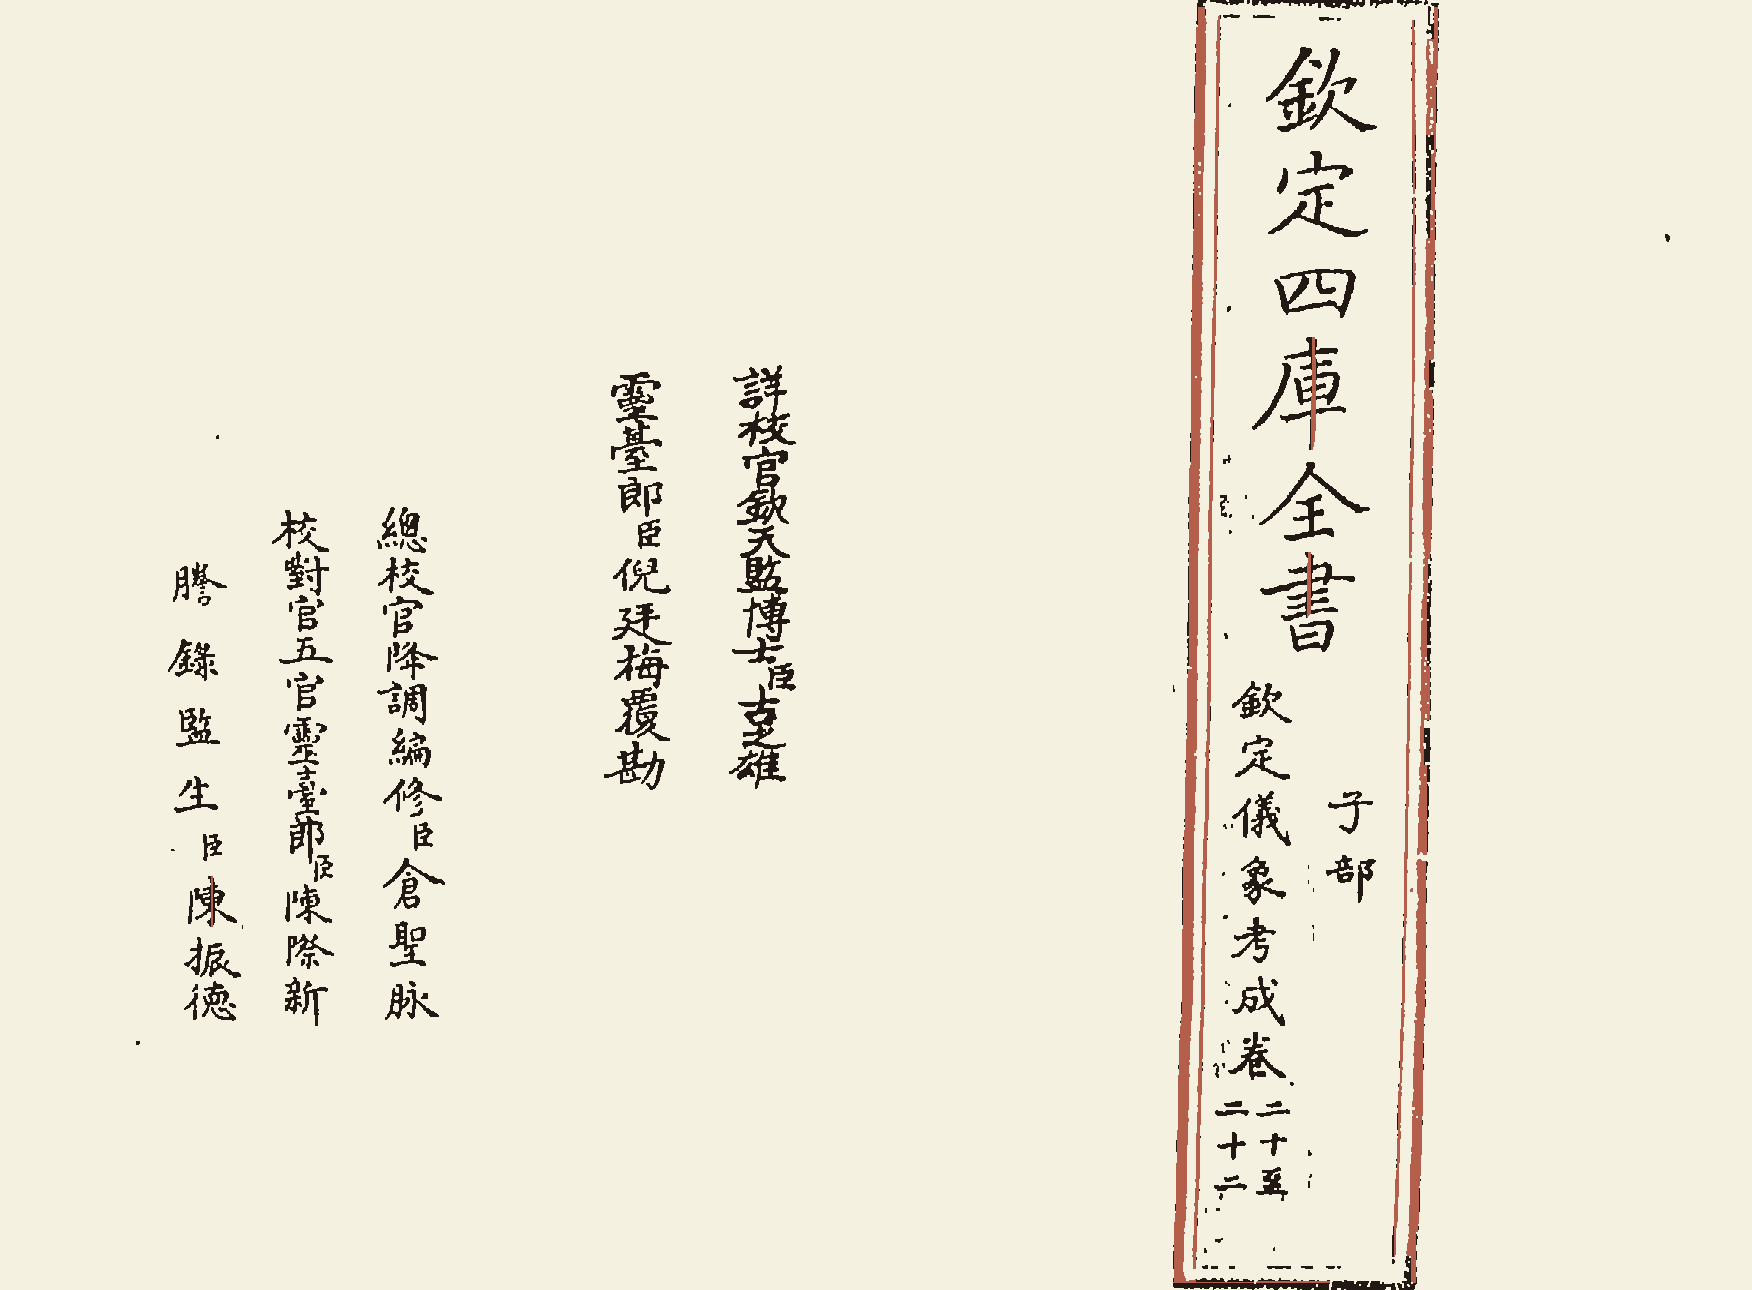
\includegraphics[width=\paperwidth,height=\paperheight,keepaspectratio]{img/1284.png}\clearpage
\begin{正文}
% ---- 册793 葉1285 ----
\SetPageNumber{1}
欽定四庫全書\换行
欽定儀象考成卷二十\换行
　恒星赤道經緯度表七\换行
　　赤道鶉首宫\双列{\右小列{黄道度附}\左小列{}}\换行
\char"200B\relax\换行
\char"200B\relax\换行
\char"200B\relax\换行
\char"200B\relax\换行
\char"200B\relax\换行
\char"200B\relax\换行
\char"200B\relax\换行
\char"200B\relax\换行
\char"200B\relax\换行
\char"200B\relax\换行
\char"200B\relax\换行
\char"200B\relax
\par
\end{正文}\clearpage
\嵌图{142.57pt}{201.98pt}{846.62pt}{585.83pt}{img/1288.png}
\begin{正文}
% ---- 册793 葉1288 图版 ----
\SetPageNumber{2}
\插图页
\char"200B\relax\换行
\char"200B\relax\换行
\char"200B\relax\换行
\char"200B\relax\换行
\char"200B\relax\换行
\char"200B\relax\换行
\char"200B\relax\换行
\char"200B\relax\换行
\char"200B\relax\换行
\char"200B\relax\换行
\char"200B\relax\换行
\char"200B\relax\换行
\char"200B\relax\换行
\char"200B\relax\换行
\char"200B\relax\换行
\char"200B\relax
\恢复丝栏\par
\end{正文}\clearpage
\嵌图{144.54pt}{203.37pt}{842.68pt}{583.06pt}{img/1289.png}
\begin{正文}
% ---- 册793 葉1289 图版 ----
\SetPageNumber{3}
\插图页
\char"200B\relax\换行
\char"200B\relax\换行
\char"200B\relax\换行
\char"200B\relax\换行
\char"200B\relax\换行
\char"200B\relax\换行
\char"200B\relax\换行
\char"200B\relax\换行
\char"200B\relax\换行
\char"200B\relax\换行
\char"200B\relax\换行
\char"200B\relax\换行
\char"200B\relax\换行
\char"200B\relax\换行
\char"200B\relax\换行
\char"200B\relax
\恢复丝栏\par
\end{正文}\clearpage
\嵌图{140.66pt}{206.04pt}{850.45pt}{577.72pt}{img/1292.png}
\begin{正文}
% ---- 册793 葉1292 图版 ----
\SetPageNumber{4}
\插图页
\char"200B\relax\换行
\char"200B\relax\换行
\char"200B\relax\换行
\char"200B\relax\换行
\char"200B\relax\换行
\char"200B\relax\换行
\char"200B\relax\换行
\char"200B\relax\换行
\char"200B\relax\换行
\char"200B\relax\换行
\char"200B\relax\换行
\char"200B\relax\换行
\char"200B\relax\换行
\char"200B\relax\换行
\char"200B\relax\换行
\char"200B\relax
\恢复丝栏\par
\end{正文}\clearpage
\嵌图{142.64pt}{200.46pt}{846.47pt}{588.87pt}{img/1293.png}
\begin{正文}
% ---- 册793 葉1293 图版 ----
\SetPageNumber{5}
\插图页
\char"200B\relax\换行
\char"200B\relax\换行
\char"200B\relax\换行
\char"200B\relax\换行
\char"200B\relax\换行
\char"200B\relax\换行
\char"200B\relax\换行
\char"200B\relax\换行
\char"200B\relax\换行
\char"200B\relax\换行
\char"200B\relax\换行
\char"200B\relax\换行
\char"200B\relax\换行
\char"200B\relax\换行
\char"200B\relax\换行
\char"200B\relax
\恢复丝栏\par
\end{正文}\clearpage
\嵌图{144.72pt}{198.69pt}{842.31pt}{592.42pt}{img/1296.png}
\begin{正文}
% ---- 册793 葉1296 图版 ----
\SetPageNumber{6}
\插图页
\char"200B\relax\换行
\char"200B\relax\换行
\char"200B\relax\换行
\char"200B\relax\换行
\char"200B\relax\换行
\char"200B\relax\换行
\char"200B\relax\换行
\char"200B\relax\换行
\char"200B\relax\换行
\char"200B\relax\换行
\char"200B\relax\换行
\char"200B\relax\换行
\char"200B\relax\换行
\char"200B\relax\换行
\char"200B\relax\换行
\char"200B\relax
\恢复丝栏\par
\end{正文}\clearpage
\嵌图{146.73pt}{198.18pt}{838.30pt}{593.43pt}{img/1297.png}
\begin{正文}
% ---- 册793 葉1297 图版 ----
\SetPageNumber{7}
\插图页
\char"200B\relax\换行
\char"200B\relax\换行
\char"200B\relax\换行
\char"200B\relax\换行
\char"200B\relax\换行
\char"200B\relax\换行
\char"200B\relax\换行
\char"200B\relax\换行
\char"200B\relax\换行
\char"200B\relax\换行
\char"200B\relax\换行
\char"200B\relax\换行
\char"200B\relax\换行
\char"200B\relax\换行
\char"200B\relax\换行
\char"200B\relax
\恢复丝栏\par
\end{正文}\clearpage
\嵌图{144.63pt}{202.87pt}{842.50pt}{584.06pt}{img/1300.png}
\begin{正文}
% ---- 册793 葉1300 图版 ----
\SetPageNumber{8}
\插图页
\char"200B\relax\换行
\char"200B\relax\换行
\char"200B\relax\换行
\char"200B\relax\换行
\char"200B\relax\换行
\char"200B\relax\换行
\char"200B\relax\换行
\char"200B\relax\换行
\char"200B\relax\换行
\char"200B\relax\换行
\char"200B\relax\换行
\char"200B\relax\换行
\char"200B\relax\换行
\char"200B\relax\换行
\char"200B\relax\换行
\char"200B\relax
\恢复丝栏\par
\end{正文}\clearpage
\嵌图{146.62pt}{202.82pt}{838.53pt}{584.14pt}{img/1301.png}
\begin{正文}
% ---- 册793 葉1301 图版 ----
\SetPageNumber{9}
\插图页
\char"200B\relax\换行
\char"200B\relax\换行
\char"200B\relax\换行
\char"200B\relax\换行
\char"200B\relax\换行
\char"200B\relax\换行
\char"200B\relax\换行
\char"200B\relax\换行
\char"200B\relax\换行
\char"200B\relax\换行
\char"200B\relax\换行
\char"200B\relax\换行
\char"200B\relax\换行
\char"200B\relax\换行
\char"200B\relax\换行
\char"200B\relax
\恢复丝栏\par
\end{正文}\clearpage
\嵌图{142.72pt}{199.59pt}{846.33pt}{590.60pt}{img/1304.png}
\begin{正文}
% ---- 册793 葉1304 图版 ----
\SetPageNumber{10}
\插图页
\char"200B\relax\换行
\char"200B\relax\换行
\char"200B\relax\换行
\char"200B\relax\换行
\char"200B\relax\换行
\char"200B\relax\换行
\char"200B\relax\换行
\char"200B\relax\换行
\char"200B\relax\换行
\char"200B\relax\换行
\char"200B\relax\换行
\char"200B\relax\换行
\char"200B\relax\换行
\char"200B\relax\换行
\char"200B\relax\换行
\char"200B\relax
\恢复丝栏\par
\end{正文}\clearpage
\嵌图{144.72pt}{200.99pt}{842.31pt}{587.80pt}{img/1305.png}
\begin{正文}
% ---- 册793 葉1305 图版 ----
\SetPageNumber{11}
\插图页
\char"200B\relax\换行
\char"200B\relax\换行
\char"200B\relax\换行
\char"200B\relax\换行
\char"200B\relax\换行
\char"200B\relax\换行
\char"200B\relax\换行
\char"200B\relax\换行
\char"200B\relax\换行
\char"200B\relax\换行
\char"200B\relax\换行
\char"200B\relax\换行
\char"200B\relax\换行
\char"200B\relax\换行
\char"200B\relax\换行
\char"200B\relax
\恢复丝栏\par
\end{正文}\clearpage
\嵌图{144.72pt}{200.06pt}{842.31pt}{589.68pt}{img/1308.png}
\begin{正文}
% ---- 册793 葉1308 图版 ----
\SetPageNumber{12}
\插图页
\char"200B\relax\换行
\char"200B\relax\换行
\char"200B\relax\换行
\char"200B\relax\换行
\char"200B\relax\换行
\char"200B\relax\换行
\char"200B\relax\换行
\char"200B\relax\换行
\char"200B\relax\换行
\char"200B\relax\换行
\char"200B\relax\换行
\char"200B\relax\换行
\char"200B\relax\换行
\char"200B\relax\换行
\char"200B\relax\换行
\char"200B\relax
\恢复丝栏\par
\end{正文}\clearpage
\嵌图{146.73pt}{199.08pt}{838.30pt}{591.64pt}{img/1309.png}
\begin{正文}
% ---- 册793 葉1309 图版 ----
\SetPageNumber{13}
\插图页
\char"200B\relax\换行
\char"200B\relax\换行
\char"200B\relax\换行
\char"200B\relax\换行
\char"200B\relax\换行
\char"200B\relax\换行
\char"200B\relax\换行
\char"200B\relax\换行
\char"200B\relax\换行
\char"200B\relax\换行
\char"200B\relax\换行
\char"200B\relax\换行
\char"200B\relax\换行
\char"200B\relax\换行
\char"200B\relax\换行
\char"200B\relax
\恢复丝栏\par
\end{正文}\clearpage
\嵌图{142.68pt}{201.95pt}{846.40pt}{585.88pt}{img/1312.png}
\begin{正文}
% ---- 册793 葉1312 图版 ----
\SetPageNumber{14}
\插图页
\char"200B\relax\换行
\char"200B\relax\换行
\char"200B\relax\换行
\char"200B\relax\换行
\char"200B\relax\换行
\char"200B\relax\换行
\char"200B\relax\换行
\char"200B\relax\换行
\char"200B\relax\换行
\char"200B\relax\换行
\char"200B\relax\换行
\char"200B\relax\换行
\char"200B\relax\换行
\char"200B\relax\换行
\char"200B\relax\换行
\char"200B\relax
\恢复丝栏\par
\end{正文}\clearpage
\嵌图{144.68pt}{199.56pt}{842.41pt}{590.66pt}{img/1313.png}
\begin{正文}
% ---- 册793 葉1313 图版 ----
\SetPageNumber{15}
\插图页
\char"200B\relax\换行
\char"200B\relax\换行
\char"200B\relax\换行
\char"200B\relax\换行
\char"200B\relax\换行
\char"200B\relax\换行
\char"200B\relax\换行
\char"200B\relax\换行
\char"200B\relax\换行
\char"200B\relax\换行
\char"200B\relax\换行
\char"200B\relax\换行
\char"200B\relax\换行
\char"200B\relax\换行
\char"200B\relax\换行
\char"200B\relax
\恢复丝栏\par
\end{正文}\clearpage
\嵌图{146.67pt}{201.49pt}{838.42pt}{586.81pt}{img/1316.png}
\begin{正文}
% ---- 册793 葉1316 图版 ----
\SetPageNumber{16}
\插图页
\char"200B\relax\换行
\char"200B\relax\换行
\char"200B\relax\换行
\char"200B\relax\换行
\char"200B\relax\换行
\char"200B\relax\换行
\char"200B\relax\换行
\char"200B\relax\换行
\char"200B\relax\换行
\char"200B\relax\换行
\char"200B\relax\换行
\char"200B\relax\换行
\char"200B\relax\换行
\char"200B\relax\换行
\char"200B\relax\换行
\char"200B\relax
\恢复丝栏\par
\end{正文}\clearpage
\嵌图{146.67pt}{198.64pt}{838.42pt}{592.51pt}{img/1317.png}
\begin{正文}
% ---- 册793 葉1317 图版 ----
\SetPageNumber{17}
\插图页
\char"200B\relax\换行
\char"200B\relax\换行
\char"200B\relax\换行
\char"200B\relax\换行
\char"200B\relax\换行
\char"200B\relax\换行
\char"200B\relax\换行
\char"200B\relax\换行
\char"200B\relax\换行
\char"200B\relax\换行
\char"200B\relax\换行
\char"200B\relax\换行
\char"200B\relax\换行
\char"200B\relax\换行
\char"200B\relax\换行
\char"200B\relax
\恢复丝栏\par
\end{正文}\clearpage
\嵌图{142.64pt}{201.01pt}{846.47pt}{587.77pt}{img/1320.png}
\begin{正文}
% ---- 册793 葉1320 图版 ----
\SetPageNumber{18}
\插图页
\char"200B\relax\换行
\char"200B\relax\换行
\char"200B\relax\换行
\char"200B\relax\换行
\char"200B\relax\换行
\char"200B\relax\换行
\char"200B\relax\换行
\char"200B\relax\换行
\char"200B\relax\换行
\char"200B\relax\换行
\char"200B\relax\换行
\char"200B\relax\换行
\char"200B\relax\换行
\char"200B\relax\换行
\char"200B\relax\换行
\char"200B\relax
\恢复丝栏\par
\end{正文}\clearpage
\嵌图{144.63pt}{202.91pt}{842.50pt}{583.97pt}{img/1321.png}
\begin{正文}
% ---- 册793 葉1321 图版 ----
\SetPageNumber{19}
\插图页
\char"200B\relax\换行
\char"200B\relax\换行
\char"200B\relax\换行
\char"200B\relax\换行
\char"200B\relax\换行
\char"200B\relax\换行
\char"200B\relax\换行
\char"200B\relax\换行
\char"200B\relax\换行
\char"200B\relax\换行
\char"200B\relax\换行
\char"200B\relax\换行
\char"200B\relax\换行
\char"200B\relax\换行
\char"200B\relax\换行
\char"200B\relax
\恢复丝栏\par
\end{正文}\clearpage
\嵌图{167.51pt}{236.84pt}{227.46pt}{584.37pt}{img/1324.png}
\begin{正文}
% ---- 册793 葉1324 ----
\SetPageNumber{20}
\char"200B\relax\换行
\char"200B\relax\换行
\char"200B\relax\换行
\char"200B\relax\换行
\char"200B\relax\换行
\char"200B\relax\换行
\char"200B\relax\换行
\char"200B\relax\换行
\char"200B\relax\换行
\char"200B\relax\换行
\char"200B\relax\换行
\char"200B\relax\换行
\char"200B\relax\换行
\char"200B\relax\换行
\char"200B\relax\换行
欽定儀象考成卷二十
\par

% ======== 卷二十一（8行21字）========
\par\end{正文}\clearpage
\chapter*{欽定儀象考成卷二十一}
\begin{正文}
% ---- 册793 葉1325 ----
\SetPageNumber{1}
欽定四庫全書\换行
欽定儀象考成卷二十一\换行
　恒星赤道經緯度表八\换行
　　赤道鶉火宫\双列{\右小列{黄道度附}\左小列{}}\换行
\char"200B\relax\换行
\char"200B\relax\换行
\char"200B\relax\换行
\char"200B\relax\换行
\char"200B\relax\换行
\char"200B\relax\换行
\char"200B\relax\换行
\char"200B\relax\换行
\char"200B\relax\换行
\char"200B\relax\换行
\char"200B\relax\换行
\char"200B\relax
\par
\end{正文}\clearpage
\嵌图{140.71pt}{198.20pt}{850.34pt}{593.39pt}{img/1328.png}
\begin{正文}
% ---- 册793 葉1328 图版 ----
\SetPageNumber{2}
\插图页
\char"200B\relax\换行
\char"200B\relax\换行
\char"200B\relax\换行
\char"200B\relax\换行
\char"200B\relax\换行
\char"200B\relax\换行
\char"200B\relax\换行
\char"200B\relax\换行
\char"200B\relax\换行
\char"200B\relax\换行
\char"200B\relax\换行
\char"200B\relax\换行
\char"200B\relax\换行
\char"200B\relax\换行
\char"200B\relax\换行
\char"200B\relax
\恢复丝栏\par
\end{正文}\clearpage
\嵌图{144.72pt}{199.15pt}{842.31pt}{591.49pt}{img/1329.png}
\begin{正文}
% ---- 册793 葉1329 图版 ----
\SetPageNumber{3}
\插图页
\char"200B\relax\换行
\char"200B\relax\换行
\char"200B\relax\换行
\char"200B\relax\换行
\char"200B\relax\换行
\char"200B\relax\换行
\char"200B\relax\换行
\char"200B\relax\换行
\char"200B\relax\换行
\char"200B\relax\换行
\char"200B\relax\换行
\char"200B\relax\换行
\char"200B\relax\换行
\char"200B\relax\换行
\char"200B\relax\换行
\char"200B\relax
\恢复丝栏\par
\end{正文}\clearpage
\嵌图{144.68pt}{201.47pt}{842.41pt}{586.86pt}{img/1332.png}
\begin{正文}
% ---- 册793 葉1332 图版 ----
\SetPageNumber{4}
\插图页
\char"200B\relax\换行
\char"200B\relax\换行
\char"200B\relax\换行
\char"200B\relax\换行
\char"200B\relax\换行
\char"200B\relax\换行
\char"200B\relax\换行
\char"200B\relax\换行
\char"200B\relax\换行
\char"200B\relax\换行
\char"200B\relax\换行
\char"200B\relax\换行
\char"200B\relax\换行
\char"200B\relax\换行
\char"200B\relax\换行
\char"200B\relax
\恢复丝栏\par
\end{正文}\clearpage
\嵌图{144.68pt}{200.51pt}{842.41pt}{588.77pt}{img/1333.png}
\begin{正文}
% ---- 册793 葉1333 图版 ----
\SetPageNumber{5}
\插图页
\char"200B\relax\换行
\char"200B\relax\换行
\char"200B\relax\换行
\char"200B\relax\换行
\char"200B\relax\换行
\char"200B\relax\换行
\char"200B\relax\换行
\char"200B\relax\换行
\char"200B\relax\换行
\char"200B\relax\换行
\char"200B\relax\换行
\char"200B\relax\换行
\char"200B\relax\换行
\char"200B\relax\换行
\char"200B\relax\换行
\char"200B\relax
\恢复丝栏\par
\end{正文}\clearpage
\嵌图{144.72pt}{200.61pt}{842.31pt}{588.57pt}{img/1336.png}
\begin{正文}
% ---- 册793 葉1336 图版 ----
\SetPageNumber{6}
\插图页
\char"200B\relax\换行
\char"200B\relax\换行
\char"200B\relax\换行
\char"200B\relax\换行
\char"200B\relax\换行
\char"200B\relax\换行
\char"200B\relax\换行
\char"200B\relax\换行
\char"200B\relax\换行
\char"200B\relax\换行
\char"200B\relax\换行
\char"200B\relax\换行
\char"200B\relax\换行
\char"200B\relax\换行
\char"200B\relax\换行
\char"200B\relax
\恢复丝栏\par
\end{正文}\clearpage
\嵌图{142.72pt}{198.19pt}{846.33pt}{593.41pt}{img/1337.png}
\begin{正文}
% ---- 册793 葉1337 图版 ----
\SetPageNumber{7}
\插图页
\char"200B\relax\换行
\char"200B\relax\换行
\char"200B\relax\换行
\char"200B\relax\换行
\char"200B\relax\换行
\char"200B\relax\换行
\char"200B\relax\换行
\char"200B\relax\换行
\char"200B\relax\换行
\char"200B\relax\换行
\char"200B\relax\换行
\char"200B\relax\换行
\char"200B\relax\换行
\char"200B\relax\换行
\char"200B\relax\换行
\char"200B\relax
\恢复丝栏\par
\end{正文}\clearpage
\嵌图{146.62pt}{200.58pt}{838.53pt}{588.64pt}{img/1340.png}
\begin{正文}
% ---- 册793 葉1340 图版 ----
\SetPageNumber{8}
\插图页
\char"200B\relax\换行
\char"200B\relax\换行
\char"200B\relax\换行
\char"200B\relax\换行
\char"200B\relax\换行
\char"200B\relax\换行
\char"200B\relax\换行
\char"200B\relax\换行
\char"200B\relax\换行
\char"200B\relax\换行
\char"200B\relax\换行
\char"200B\relax\换行
\char"200B\relax\换行
\char"200B\relax\换行
\char"200B\relax\换行
\char"200B\relax
\恢复丝栏\par
\end{正文}\clearpage
\嵌图{144.63pt}{199.12pt}{842.50pt}{591.55pt}{img/1341.png}
\begin{正文}
% ---- 册793 葉1341 图版 ----
\SetPageNumber{9}
\插图页
\char"200B\relax\换行
\char"200B\relax\换行
\char"200B\relax\换行
\char"200B\relax\换行
\char"200B\relax\换行
\char"200B\relax\换行
\char"200B\relax\换行
\char"200B\relax\换行
\char"200B\relax\换行
\char"200B\relax\换行
\char"200B\relax\换行
\char"200B\relax\换行
\char"200B\relax\换行
\char"200B\relax\换行
\char"200B\relax\换行
\char"200B\relax
\恢复丝栏\par
\end{正文}\clearpage
\嵌图{142.64pt}{200.11pt}{846.47pt}{589.58pt}{img/1344.png}
\begin{正文}
% ---- 册793 葉1344 图版 ----
\SetPageNumber{10}
\插图页
\char"200B\relax\换行
\char"200B\relax\换行
\char"200B\relax\换行
\char"200B\relax\换行
\char"200B\relax\换行
\char"200B\relax\换行
\char"200B\relax\换行
\char"200B\relax\换行
\char"200B\relax\换行
\char"200B\relax\换行
\char"200B\relax\换行
\char"200B\relax\换行
\char"200B\relax\换行
\char"200B\relax\换行
\char"200B\relax\换行
\char"200B\relax
\恢复丝栏\par
\end{正文}\clearpage
\嵌图{146.62pt}{198.67pt}{838.53pt}{592.45pt}{img/1345.png}
\begin{正文}
% ---- 册793 葉1345 图版 ----
\SetPageNumber{11}
\插图页
\char"200B\relax\换行
\char"200B\relax\换行
\char"200B\relax\换行
\char"200B\relax\换行
\char"200B\relax\换行
\char"200B\relax\换行
\char"200B\relax\换行
\char"200B\relax\换行
\char"200B\relax\换行
\char"200B\relax\换行
\char"200B\relax\换行
\char"200B\relax\换行
\char"200B\relax\换行
\char"200B\relax\换行
\char"200B\relax\换行
\char"200B\relax
\恢复丝栏\par
\end{正文}\clearpage
\嵌图{146.62pt}{202.94pt}{838.53pt}{583.90pt}{img/1348.png}
\begin{正文}
% ---- 册793 葉1348 图版 ----
\SetPageNumber{12}
\插图页
\char"200B\relax\换行
\char"200B\relax\换行
\char"200B\relax\换行
\char"200B\relax\换行
\char"200B\relax\换行
\char"200B\relax\换行
\char"200B\relax\换行
\char"200B\relax\换行
\char"200B\relax\换行
\char"200B\relax\换行
\char"200B\relax\换行
\char"200B\relax\换行
\char"200B\relax\换行
\char"200B\relax\换行
\char"200B\relax\换行
\char"200B\relax
\恢复丝栏\par
\end{正文}\clearpage
\嵌图{146.62pt}{201.02pt}{838.53pt}{587.76pt}{img/1349.png}
\begin{正文}
% ---- 册793 葉1349 图版 ----
\SetPageNumber{13}
\插图页
\char"200B\relax\换行
\char"200B\relax\换行
\char"200B\relax\换行
\char"200B\relax\换行
\char"200B\relax\换行
\char"200B\relax\换行
\char"200B\relax\换行
\char"200B\relax\换行
\char"200B\relax\换行
\char"200B\relax\换行
\char"200B\relax\换行
\char"200B\relax\换行
\char"200B\relax\换行
\char"200B\relax\换行
\char"200B\relax\换行
\char"200B\relax
\恢复丝栏\par
\end{正文}\clearpage
\嵌图{140.66pt}{202.49pt}{850.45pt}{584.80pt}{img/1352.png}
\begin{正文}
% ---- 册793 葉1352 图版 ----
\SetPageNumber{14}
\插图页
\char"200B\relax\换行
\char"200B\relax\换行
\char"200B\relax\换行
\char"200B\relax\换行
\char"200B\relax\换行
\char"200B\relax\换行
\char"200B\relax\换行
\char"200B\relax\换行
\char"200B\relax\换行
\char"200B\relax\换行
\char"200B\relax\换行
\char"200B\relax\换行
\char"200B\relax\换行
\char"200B\relax\换行
\char"200B\relax\换行
\char"200B\relax
\恢复丝栏\par
\end{正文}\clearpage
\嵌图{142.64pt}{200.08pt}{846.47pt}{589.63pt}{img/1353.png}
\begin{正文}
% ---- 册793 葉1353 图版 ----
\SetPageNumber{15}
\插图页
\char"200B\relax\换行
\char"200B\relax\换行
\char"200B\relax\换行
\char"200B\relax\换行
\char"200B\relax\换行
\char"200B\relax\换行
\char"200B\relax\换行
\char"200B\relax\换行
\char"200B\relax\换行
\char"200B\relax\换行
\char"200B\relax\换行
\char"200B\relax\换行
\char"200B\relax\换行
\char"200B\relax\换行
\char"200B\relax\换行
\char"200B\relax
\恢复丝栏\par
\end{正文}\clearpage
\嵌图{140.66pt}{201.00pt}{850.45pt}{587.79pt}{img/1356.png}
\begin{正文}
% ---- 册793 葉1356 图版 ----
\SetPageNumber{16}
\插图页
\char"200B\relax\换行
\char"200B\relax\换行
\char"200B\relax\换行
\char"200B\relax\换行
\char"200B\relax\换行
\char"200B\relax\换行
\char"200B\relax\换行
\char"200B\relax\换行
\char"200B\relax\换行
\char"200B\relax\换行
\char"200B\relax\换行
\char"200B\relax\换行
\char"200B\relax\换行
\char"200B\relax\换行
\char"200B\relax\换行
\char"200B\relax
\恢复丝栏\par
\end{正文}\clearpage
\嵌图{142.64pt}{201.88pt}{846.47pt}{586.02pt}{img/1357.png}
\begin{正文}
% ---- 册793 葉1357 图版 ----
\SetPageNumber{17}
\插图页
\char"200B\relax\换行
\char"200B\relax\换行
\char"200B\relax\换行
\char"200B\relax\换行
\char"200B\relax\换行
\char"200B\relax\换行
\char"200B\relax\换行
\char"200B\relax\换行
\char"200B\relax\换行
\char"200B\relax\换行
\char"200B\relax\换行
\char"200B\relax\换行
\char"200B\relax\换行
\char"200B\relax\换行
\char"200B\relax\换行
\char"200B\relax
\恢复丝栏\par
\end{正文}\clearpage
\嵌图{144.63pt}{199.13pt}{842.50pt}{591.52pt}{img/1360.png}
\begin{正文}
% ---- 册793 葉1360 图版 ----
\SetPageNumber{18}
\插图页
\char"200B\relax\换行
\char"200B\relax\换行
\char"200B\relax\换行
\char"200B\relax\换行
\char"200B\relax\换行
\char"200B\relax\换行
\char"200B\relax\换行
\char"200B\relax\换行
\char"200B\relax\换行
\char"200B\relax\换行
\char"200B\relax\换行
\char"200B\relax\换行
\char"200B\relax\换行
\char"200B\relax\换行
\char"200B\relax\换行
\char"200B\relax
\恢复丝栏\par
\end{正文}\clearpage
\嵌图{142.64pt}{200.57pt}{846.47pt}{588.65pt}{img/1361.png}
\begin{正文}
% ---- 册793 葉1361 图版 ----
\SetPageNumber{19}
\插图页
\char"200B\relax\换行
\char"200B\relax\换行
\char"200B\relax\换行
\char"200B\relax\换行
\char"200B\relax\换行
\char"200B\relax\换行
\char"200B\relax\换行
\char"200B\relax\换行
\char"200B\relax\换行
\char"200B\relax\换行
\char"200B\relax\换行
\char"200B\relax\换行
\char"200B\relax\换行
\char"200B\relax\换行
\char"200B\relax\换行
\char"200B\relax
\恢复丝栏\par
\end{正文}\clearpage
\嵌图{144.63pt}{200.99pt}{842.50pt}{587.82pt}{img/1364.png}
\begin{正文}
% ---- 册793 葉1364 图版 ----
\SetPageNumber{20}
\插图页
\char"200B\relax\换行
\char"200B\relax\换行
\char"200B\relax\换行
\char"200B\relax\换行
\char"200B\relax\换行
\char"200B\relax\换行
\char"200B\relax\换行
\char"200B\relax\换行
\char"200B\relax\换行
\char"200B\relax\换行
\char"200B\relax\换行
\char"200B\relax\换行
\char"200B\relax\换行
\char"200B\relax\换行
\char"200B\relax\换行
\char"200B\relax
\恢复丝栏\par
\end{正文}\clearpage
\嵌图{144.63pt}{199.08pt}{842.50pt}{591.64pt}{img/1365.png}
\begin{正文}
% ---- 册793 葉1365 图版 ----
\SetPageNumber{21}
\插图页
\char"200B\relax\换行
\char"200B\relax\换行
\char"200B\relax\换行
\char"200B\relax\换行
\char"200B\relax\换行
\char"200B\relax\换行
\char"200B\relax\换行
\char"200B\relax\换行
\char"200B\relax\换行
\char"200B\relax\换行
\char"200B\relax\换行
\char"200B\relax\换行
\char"200B\relax\换行
\char"200B\relax\换行
\char"200B\relax\换行
\char"200B\relax
\恢复丝栏\par
\end{正文}\clearpage
\嵌图{174.32pt}{212.19pt}{169.63pt}{580.64pt}{img/1368.png}
\begin{正文}
% ---- 册793 葉1368 ----
\SetPageNumber{22}
\char"200B\relax\换行
\char"200B\relax\换行
\char"200B\relax\换行
\char"200B\relax\换行
\char"200B\relax\换行
\char"200B\relax\换行
\char"200B\relax\换行
\char"200B\relax\换行
\char"200B\relax\换行
\char"200B\relax\换行
\char"200B\relax\换行
\char"200B\relax\换行
\char"200B\relax\换行
\char"200B\relax\换行
\char"200B\relax\换行
欽定儀象考成卷二十一
\par

% ======== 卷二十二（8行21字）========
\par\end{正文}\clearpage
\chapter*{欽定儀象考成卷二十二}
\begin{正文}
% ---- 册793 葉1369 ----
\SetPageNumber{1}
欽定四庫全書\换行
欽定儀象考成卷二十二\换行
　恒星赤道經緯度表九\换行
　　赤道鶉尾宫\双列{\右小列{黄道度附}\左小列{}}\换行
\char"200B\relax\换行
\char"200B\relax\换行
\char"200B\relax\换行
\char"200B\relax\换行
\char"200B\relax\换行
\char"200B\relax\换行
\char"200B\relax\换行
\char"200B\relax\换行
\char"200B\relax\换行
\char"200B\relax\换行
\char"200B\relax\换行
\char"200B\relax
\par
\end{正文}\clearpage
\嵌图{144.63pt}{198.62pt}{842.50pt}{592.56pt}{img/1372.png}
\begin{正文}
% ---- 册793 葉1372 图版 ----
\SetPageNumber{2}
\插图页
\char"200B\relax\换行
\char"200B\relax\换行
\char"200B\relax\换行
\char"200B\relax\换行
\char"200B\relax\换行
\char"200B\relax\换行
\char"200B\relax\换行
\char"200B\relax\换行
\char"200B\relax\换行
\char"200B\relax\换行
\char"200B\relax\换行
\char"200B\relax\换行
\char"200B\relax\换行
\char"200B\relax\换行
\char"200B\relax\换行
\char"200B\relax
\恢复丝栏\par
\end{正文}\clearpage
\嵌图{144.63pt}{200.97pt}{842.50pt}{587.86pt}{img/1373.png}
\begin{正文}
% ---- 册793 葉1373 图版 ----
\SetPageNumber{3}
\插图页
\char"200B\relax\换行
\char"200B\relax\换行
\char"200B\relax\换行
\char"200B\relax\换行
\char"200B\relax\换行
\char"200B\relax\换行
\char"200B\relax\换行
\char"200B\relax\换行
\char"200B\relax\换行
\char"200B\relax\换行
\char"200B\relax\换行
\char"200B\relax\换行
\char"200B\relax\换行
\char"200B\relax\换行
\char"200B\relax\换行
\char"200B\relax
\恢复丝栏\par
\end{正文}\clearpage
\嵌图{142.64pt}{199.65pt}{846.47pt}{590.49pt}{img/1376.png}
\begin{正文}
% ---- 册793 葉1376 图版 ----
\SetPageNumber{4}
\插图页
\char"200B\relax\换行
\char"200B\relax\换行
\char"200B\relax\换行
\char"200B\relax\换行
\char"200B\relax\换行
\char"200B\relax\换行
\char"200B\relax\换行
\char"200B\relax\换行
\char"200B\relax\换行
\char"200B\relax\换行
\char"200B\relax\换行
\char"200B\relax\换行
\char"200B\relax\换行
\char"200B\relax\换行
\char"200B\relax\换行
\char"200B\relax
\恢复丝栏\par
\end{正文}\clearpage
\嵌图{142.64pt}{200.56pt}{846.47pt}{588.68pt}{img/1377.png}
\begin{正文}
% ---- 册793 葉1377 图版 ----
\SetPageNumber{5}
\插图页
\char"200B\relax\换行
\char"200B\relax\换行
\char"200B\relax\换行
\char"200B\relax\换行
\char"200B\relax\换行
\char"200B\relax\换行
\char"200B\relax\换行
\char"200B\relax\换行
\char"200B\relax\换行
\char"200B\relax\换行
\char"200B\relax\换行
\char"200B\relax\换行
\char"200B\relax\换行
\char"200B\relax\换行
\char"200B\relax\换行
\char"200B\relax
\恢复丝栏\par
\end{正文}\clearpage
\嵌图{146.62pt}{201.07pt}{838.53pt}{587.66pt}{img/1380.png}
\begin{正文}
% ---- 册793 葉1380 图版 ----
\SetPageNumber{6}
\插图页
\char"200B\relax\换行
\char"200B\relax\换行
\char"200B\relax\换行
\char"200B\relax\换行
\char"200B\relax\换行
\char"200B\relax\换行
\char"200B\relax\换行
\char"200B\relax\换行
\char"200B\relax\换行
\char"200B\relax\换行
\char"200B\relax\换行
\char"200B\relax\换行
\char"200B\relax\换行
\char"200B\relax\换行
\char"200B\relax\换行
\char"200B\relax
\恢复丝栏\par
\end{正文}\clearpage
\嵌图{144.63pt}{199.13pt}{842.50pt}{591.54pt}{img/1381.png}
\begin{正文}
% ---- 册793 葉1381 图版 ----
\SetPageNumber{7}
\插图页
\char"200B\relax\换行
\char"200B\relax\换行
\char"200B\relax\换行
\char"200B\relax\换行
\char"200B\relax\换行
\char"200B\relax\换行
\char"200B\relax\换行
\char"200B\relax\换行
\char"200B\relax\换行
\char"200B\relax\换行
\char"200B\relax\换行
\char"200B\relax\换行
\char"200B\relax\换行
\char"200B\relax\换行
\char"200B\relax\换行
\char"200B\relax
\恢复丝栏\par
\end{正文}\clearpage
\嵌图{146.56pt}{202.88pt}{838.64pt}{584.02pt}{img/1384.png}
\begin{正文}
% ---- 册793 葉1384 图版 ----
\SetPageNumber{8}
\插图页
\char"200B\relax\换行
\char"200B\relax\换行
\char"200B\relax\换行
\char"200B\relax\换行
\char"200B\relax\换行
\char"200B\relax\换行
\char"200B\relax\换行
\char"200B\relax\换行
\char"200B\relax\换行
\char"200B\relax\换行
\char"200B\relax\换行
\char"200B\relax\换行
\char"200B\relax\换行
\char"200B\relax\换行
\char"200B\relax\换行
\char"200B\relax
\恢复丝栏\par
\end{正文}\clearpage
\嵌图{146.56pt}{202.40pt}{838.64pt}{584.98pt}{img/1385.png}
\begin{正文}
% ---- 册793 葉1385 图版 ----
\SetPageNumber{9}
\插图页
\char"200B\relax\换行
\char"200B\relax\换行
\char"200B\relax\换行
\char"200B\relax\换行
\char"200B\relax\换行
\char"200B\relax\换行
\char"200B\relax\换行
\char"200B\relax\换行
\char"200B\relax\换行
\char"200B\relax\换行
\char"200B\relax\换行
\char"200B\relax\换行
\char"200B\relax\换行
\char"200B\relax\换行
\char"200B\relax\换行
\char"200B\relax
\恢复丝栏\par
\end{正文}\clearpage
\嵌图{148.54pt}{201.96pt}{834.68pt}{585.86pt}{img/1388.png}
\begin{正文}
% ---- 册793 葉1388 图版 ----
\SetPageNumber{10}
\插图页
\char"200B\relax\换行
\char"200B\relax\换行
\char"200B\relax\换行
\char"200B\relax\换行
\char"200B\relax\换行
\char"200B\relax\换行
\char"200B\relax\换行
\char"200B\relax\换行
\char"200B\relax\换行
\char"200B\relax\换行
\char"200B\relax\换行
\char"200B\relax\换行
\char"200B\relax\换行
\char"200B\relax\换行
\char"200B\relax\换行
\char"200B\relax
\恢复丝栏\par
\end{正文}\clearpage
\嵌图{144.59pt}{199.08pt}{842.59pt}{591.63pt}{img/1389.png}
\begin{正文}
% ---- 册793 葉1389 图版 ----
\SetPageNumber{11}
\插图页
\char"200B\relax\换行
\char"200B\relax\换行
\char"200B\relax\换行
\char"200B\relax\换行
\char"200B\relax\换行
\char"200B\relax\换行
\char"200B\relax\换行
\char"200B\relax\换行
\char"200B\relax\换行
\char"200B\relax\换行
\char"200B\relax\换行
\char"200B\relax\换行
\char"200B\relax\换行
\char"200B\relax\换行
\char"200B\relax\换行
\char"200B\relax
\恢复丝栏\par
\end{正文}\clearpage
\嵌图{146.62pt}{201.03pt}{838.53pt}{587.73pt}{img/1392.png}
\begin{正文}
% ---- 册793 葉1392 图版 ----
\SetPageNumber{12}
\插图页
\char"200B\relax\换行
\char"200B\relax\换行
\char"200B\relax\换行
\char"200B\relax\换行
\char"200B\relax\换行
\char"200B\relax\换行
\char"200B\relax\换行
\char"200B\relax\换行
\char"200B\relax\换行
\char"200B\relax\换行
\char"200B\relax\换行
\char"200B\relax\换行
\char"200B\relax\换行
\char"200B\relax\换行
\char"200B\relax\换行
\char"200B\relax
\恢复丝栏\par
\end{正文}\clearpage
\嵌图{146.62pt}{201.03pt}{838.53pt}{587.73pt}{img/1393.png}
\begin{正文}
% ---- 册793 葉1393 图版 ----
\SetPageNumber{13}
\插图页
\char"200B\relax\换行
\char"200B\relax\换行
\char"200B\relax\换行
\char"200B\relax\换行
\char"200B\relax\换行
\char"200B\relax\换行
\char"200B\relax\换行
\char"200B\relax\换行
\char"200B\relax\换行
\char"200B\relax\换行
\char"200B\relax\换行
\char"200B\relax\换行
\char"200B\relax\换行
\char"200B\relax\换行
\char"200B\relax\换行
\char"200B\relax
\恢复丝栏\par
\end{正文}\clearpage
\嵌图{142.64pt}{201.90pt}{846.47pt}{585.99pt}{img/1396.png}
\begin{正文}
% ---- 册793 葉1396 图版 ----
\SetPageNumber{14}
\插图页
\char"200B\relax\换行
\char"200B\relax\换行
\char"200B\relax\换行
\char"200B\relax\换行
\char"200B\relax\换行
\char"200B\relax\换行
\char"200B\relax\换行
\char"200B\relax\换行
\char"200B\relax\换行
\char"200B\relax\换行
\char"200B\relax\换行
\char"200B\relax\换行
\char"200B\relax\换行
\char"200B\relax\换行
\char"200B\relax\换行
\char"200B\relax
\恢复丝栏\par
\end{正文}\clearpage
\嵌图{146.62pt}{201.43pt}{838.53pt}{586.93pt}{img/1397.png}
\begin{正文}
% ---- 册793 葉1397 图版 ----
\SetPageNumber{15}
\插图页
\char"200B\relax\换行
\char"200B\relax\换行
\char"200B\relax\换行
\char"200B\relax\换行
\char"200B\relax\换行
\char"200B\relax\换行
\char"200B\relax\换行
\char"200B\relax\换行
\char"200B\relax\换行
\char"200B\relax\换行
\char"200B\relax\换行
\char"200B\relax\换行
\char"200B\relax\换行
\char"200B\relax\换行
\char"200B\relax\换行
\char"200B\relax
\恢复丝栏\par
\end{正文}\clearpage
\嵌图{144.63pt}{199.61pt}{842.50pt}{590.58pt}{img/1400.png}
\begin{正文}
% ---- 册793 葉1400 图版 ----
\SetPageNumber{16}
\插图页
\char"200B\relax\换行
\char"200B\relax\换行
\char"200B\relax\换行
\char"200B\relax\换行
\char"200B\relax\换行
\char"200B\relax\换行
\char"200B\relax\换行
\char"200B\relax\换行
\char"200B\relax\换行
\char"200B\relax\换行
\char"200B\relax\换行
\char"200B\relax\换行
\char"200B\relax\换行
\char"200B\relax\换行
\char"200B\relax\换行
\char"200B\relax
\恢复丝栏\par
\end{正文}\clearpage
\嵌图{148.61pt}{198.60pt}{834.55pt}{592.58pt}{img/1401.png}
\begin{正文}
% ---- 册793 葉1401 图版 ----
\SetPageNumber{17}
\插图页
\char"200B\relax\换行
\char"200B\relax\换行
\char"200B\relax\换行
\char"200B\relax\换行
\char"200B\relax\换行
\char"200B\relax\换行
\char"200B\relax\换行
\char"200B\relax\换行
\char"200B\relax\换行
\char"200B\relax\换行
\char"200B\relax\换行
\char"200B\relax\换行
\char"200B\relax\换行
\char"200B\relax\换行
\char"200B\relax\换行
\char"200B\relax
\恢复丝栏\par
\end{正文}\clearpage
\嵌图{142.68pt}{200.05pt}{846.40pt}{589.69pt}{img/1404.png}
\begin{正文}
% ---- 册793 葉1404 图版 ----
\SetPageNumber{18}
\插图页
\char"200B\relax\换行
\char"200B\relax\换行
\char"200B\relax\换行
\char"200B\relax\换行
\char"200B\relax\换行
\char"200B\relax\换行
\char"200B\relax\换行
\char"200B\relax\换行
\char"200B\relax\换行
\char"200B\relax\换行
\char"200B\relax\换行
\char"200B\relax\换行
\char"200B\relax\换行
\char"200B\relax\换行
\char"200B\relax\换行
\char"200B\relax
\恢复丝栏\par
\end{正文}\clearpage
\嵌图{144.68pt}{197.70pt}{842.41pt}{594.38pt}{img/1405.png}
\begin{正文}
% ---- 册793 葉1405 图版 ----
\SetPageNumber{19}
\插图页
\char"200B\relax\换行
\char"200B\relax\换行
\char"200B\relax\换行
\char"200B\relax\换行
\char"200B\relax\换行
\char"200B\relax\换行
\char"200B\relax\换行
\char"200B\relax\换行
\char"200B\relax\换行
\char"200B\relax\换行
\char"200B\relax\换行
\char"200B\relax\换行
\char"200B\relax\换行
\char"200B\relax\换行
\char"200B\relax\换行
\char"200B\relax
\恢复丝栏\par
\end{正文}\clearpage
\嵌图{143.22pt}{214.95pt}{404.80pt}{577.88pt}{img/1408.png}
\begin{正文}
% ---- 册793 葉1408 ----
\SetPageNumber{20}
\插图页
\char"200B\relax\换行
\char"200B\relax\换行
\char"200B\relax\换行
\char"200B\relax\换行
\char"200B\relax\换行
\char"200B\relax\换行
\char"200B\relax\换行
\char"200B\relax\换行
\恢复丝栏
\char"200B\relax\换行
\char"200B\relax\换行
\char"200B\relax\换行
\char"200B\relax\换行
\char"200B\relax\换行
\char"200B\relax\换行
\char"200B\relax\换行
欽定儀象考成卷二十二
\par

% ======== 卷二十三（8行21字）========
\par\end{正文}\clearpage
\chapter*{欽定儀象考成卷二十三}
\begin{正文}
\end{正文}\clearpage

  \input{parts/part14}
  % ======== 卷二十七（8行21字）========
\chapter*{欽定儀象考成卷二十七}
\begin{正文}
\end{正文}\clearpage
\thispagestyle{empty}\noindent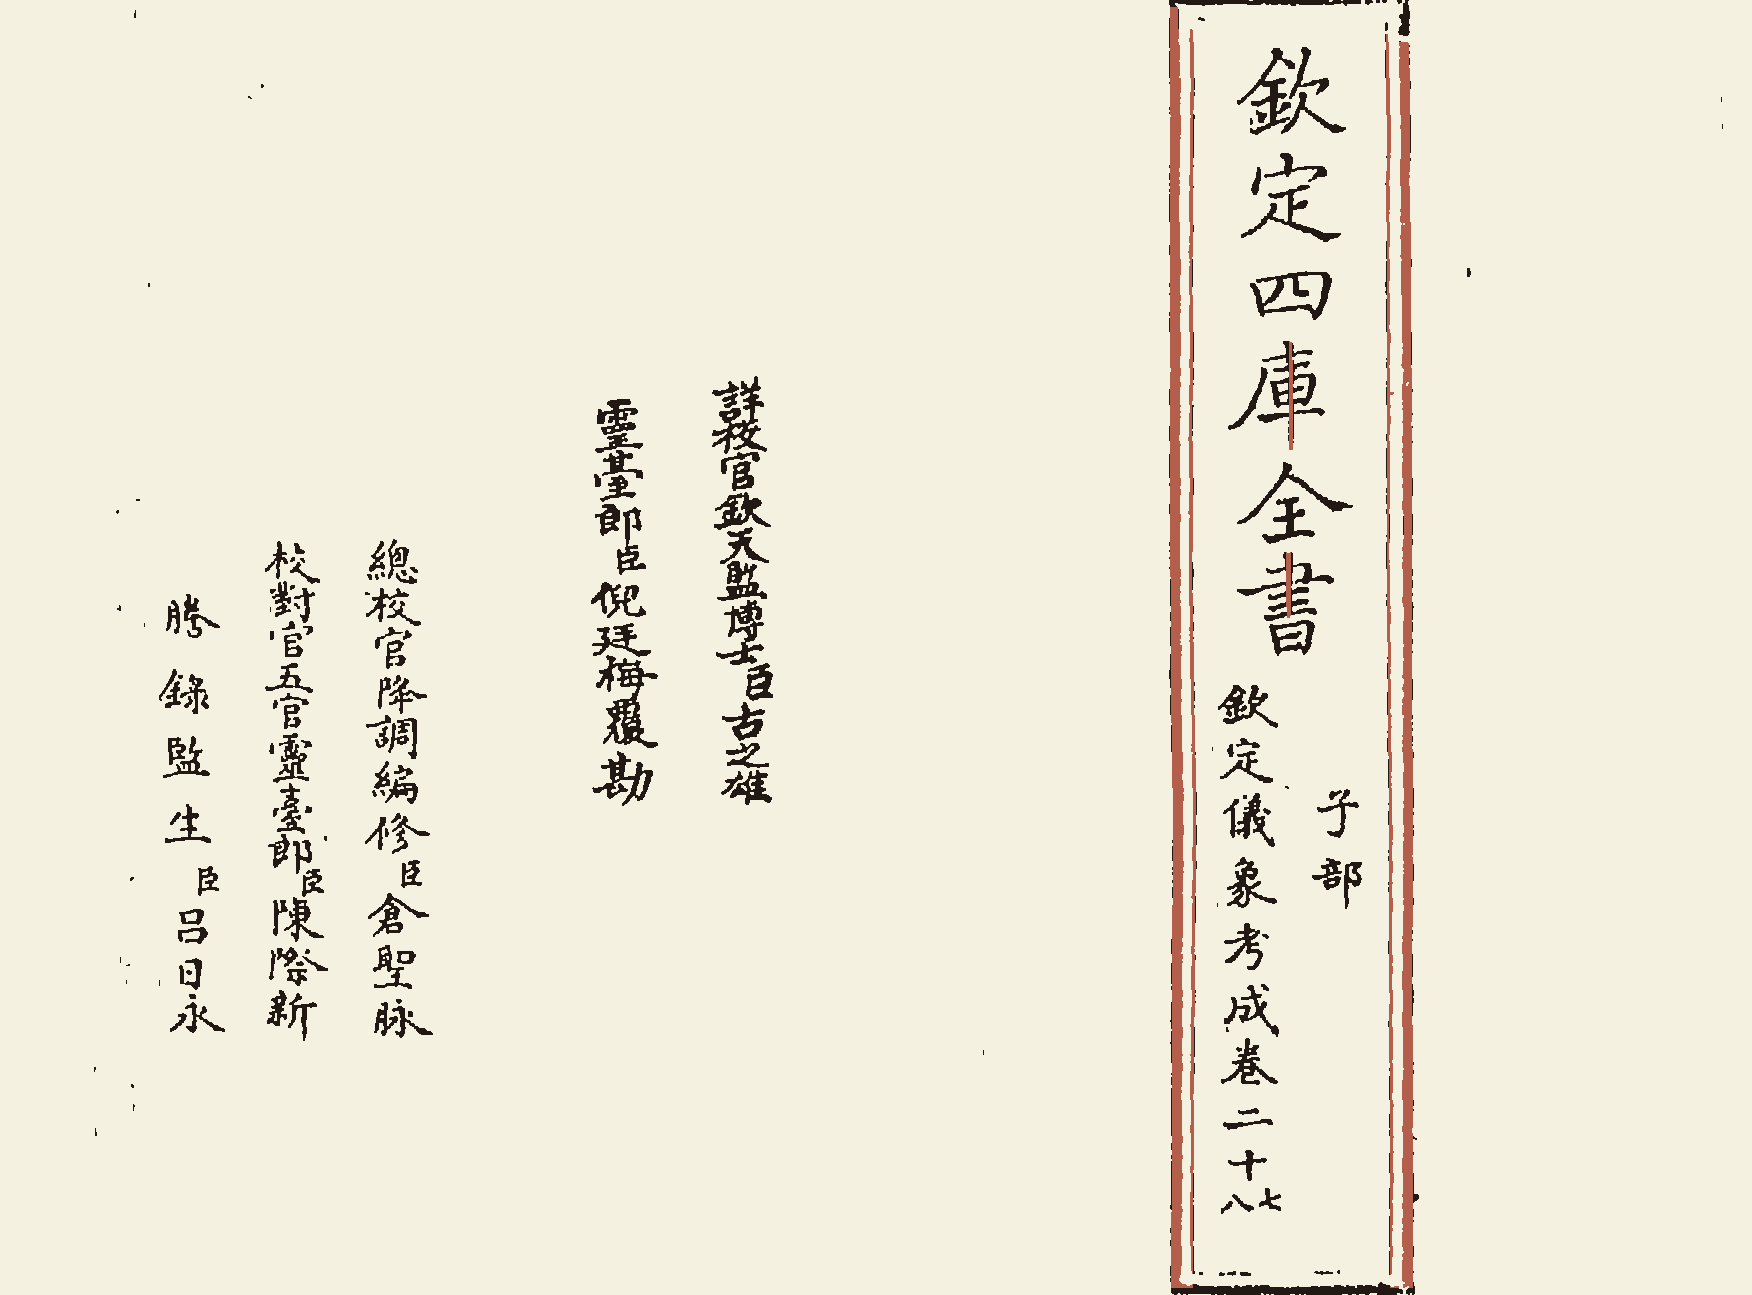
\includegraphics[width=\paperwidth,height=\paperheight,keepaspectratio]{img/1668.png}\clearpage
\begin{正文}
% ---- 册793 葉1669 ----
\SetPageNumber{1}
欽定四庫全書\换行
欽定儀象考成卷二十七\换行
　天漢經緯度表一\换行
　　黄道北天漢度\换行
\char"200B\relax\换行
\char"200B\relax\换行
\char"200B\relax\换行
\char"200B\relax\换行
\char"200B\relax\换行
\char"200B\relax\换行
\char"200B\relax\换行
\char"200B\relax\换行
\char"200B\relax\换行
\char"200B\relax\换行
\char"200B\relax\换行
\char"200B\relax
\par
% ---- 册793 葉1672 ----
　　天漢黄赤經緯度表\换行
晉書天文志云天漢起東方經箕尾之間謂之漢津乃\换行
分為二道其南經傳説魚天籥天弁河鼓其北經龜貫\换行
箕下次絡南斗魁左旗至天津下而合南道乃西南行\换行
又分夾瓠𤓰絡人星杵造父螣蛇王良附路閣道北端\换行
大陵天船卷舌而南行絡五車經北河之南入東井水\换行
位而東南行絡南河闕邱天狗天記天稷至七星南而\换行
没明史天文志云近年浮海之人至赤道以南見雲漢\换行
過天狗之墟抵天社海石之南踰南船帶海山貫十字\换行
\抬头[1]架蜜蜂傍馬腹經南門絡三角龜杵而屬扵尾宿是為帶\换行
\抬头[1]天一周靈䑓儀象志天漢經緯度分列黄道南北赤道南\换行
\抬头[1]北四表與明史合但不按宮次或分二界或分三界或分\换行
\抬头[1]四界逐度列表其分合曲折之處尚有未詳今亦分黄赤\换行
\抬头[1]南北四表而各按宮次分南界北界南之北界北之南界\换行
各列四層其分合既為明晰至其曲折之處經緯或有\换行
不同又扵每度之間細分列表按數圖之庶合懸象云
\par
\end{正文}\clearpage
\嵌图{146.56pt}{202.31pt}{838.64pt}{585.16pt}{img/1673.png}
\begin{正文}
% ---- 册793 葉1673 图版 ----
\SetPageNumber{3}
\插图页
\char"200B\relax\换行
\char"200B\relax\换行
\char"200B\relax\换行
\char"200B\relax\换行
\char"200B\relax\换行
\char"200B\relax\换行
\char"200B\relax\换行
\char"200B\relax\换行
\char"200B\relax\换行
\char"200B\relax\换行
\char"200B\relax\换行
\char"200B\relax\换行
\char"200B\relax\换行
\char"200B\relax\换行
\char"200B\relax\换行
\char"200B\relax
\恢复丝栏\par
\end{正文}\clearpage
\嵌图{144.59pt}{205.10pt}{842.59pt}{579.59pt}{img/1676.png}
\begin{正文}
% ---- 册793 葉1676 图版 ----
\SetPageNumber{4}
\插图页
\char"200B\relax\换行
\char"200B\relax\换行
\char"200B\relax\换行
\char"200B\relax\换行
\char"200B\relax\换行
\char"200B\relax\换行
\char"200B\relax\换行
\char"200B\relax\换行
\char"200B\relax\换行
\char"200B\relax\换行
\char"200B\relax\换行
\char"200B\relax\换行
\char"200B\relax\换行
\char"200B\relax\换行
\char"200B\relax\换行
\char"200B\relax
\恢复丝栏\par
\end{正文}\clearpage
\嵌图{150.52pt}{204.54pt}{830.72pt}{580.72pt}{img/1677.png}
\begin{正文}
% ---- 册793 葉1677 图版 ----
\SetPageNumber{5}
\插图页
\char"200B\relax\换行
\char"200B\relax\换行
\char"200B\relax\换行
\char"200B\relax\换行
\char"200B\relax\换行
\char"200B\relax\换行
\char"200B\relax\换行
\char"200B\relax\换行
\char"200B\relax\换行
\char"200B\relax\换行
\char"200B\relax\换行
\char"200B\relax\换行
\char"200B\relax\换行
\char"200B\relax\换行
\char"200B\relax\换行
\char"200B\relax
\恢复丝栏\par
\end{正文}\clearpage
\嵌图{146.62pt}{204.17pt}{838.53pt}{581.46pt}{img/1680.png}
\begin{正文}
% ---- 册793 葉1680 图版 ----
\SetPageNumber{6}
\插图页
\char"200B\relax\换行
\char"200B\relax\换行
\char"200B\relax\换行
\char"200B\relax\换行
\char"200B\relax\换行
\char"200B\relax\换行
\char"200B\relax\换行
\char"200B\relax\换行
\char"200B\relax\换行
\char"200B\relax\换行
\char"200B\relax\换行
\char"200B\relax\换行
\char"200B\relax\换行
\char"200B\relax\换行
\char"200B\relax\换行
\char"200B\relax
\恢复丝栏\par
\end{正文}\clearpage
\嵌图{144.63pt}{202.37pt}{842.50pt}{585.05pt}{img/1681.png}
\begin{正文}
% ---- 册793 葉1681 图版 ----
\SetPageNumber{7}
\插图页
\char"200B\relax\换行
\char"200B\relax\换行
\char"200B\relax\换行
\char"200B\relax\换行
\char"200B\relax\换行
\char"200B\relax\换行
\char"200B\relax\换行
\char"200B\relax\换行
\char"200B\relax\换行
\char"200B\relax\换行
\char"200B\relax\换行
\char"200B\relax\换行
\char"200B\relax\换行
\char"200B\relax\换行
\char"200B\relax\换行
\char"200B\relax
\恢复丝栏\par
\end{正文}\clearpage
\嵌图{146.56pt}{205.07pt}{838.64pt}{579.65pt}{img/1684.png}
\begin{正文}
% ---- 册793 葉1684 图版 ----
\SetPageNumber{8}
\插图页
\char"200B\relax\换行
\char"200B\relax\换行
\char"200B\relax\换行
\char"200B\relax\换行
\char"200B\relax\换行
\char"200B\relax\换行
\char"200B\relax\换行
\char"200B\relax\换行
\char"200B\relax\换行
\char"200B\relax\换行
\char"200B\relax\换行
\char"200B\relax\换行
\char"200B\relax\换行
\char"200B\relax\换行
\char"200B\relax\换行
\char"200B\relax
\恢复丝栏\par
\end{正文}\clearpage
\嵌图{146.56pt}{203.63pt}{838.64pt}{582.54pt}{img/1685.png}
\begin{正文}
% ---- 册793 葉1685 图版 ----
\SetPageNumber{9}
\插图页
\char"200B\relax\换行
\char"200B\relax\换行
\char"200B\relax\换行
\char"200B\relax\换行
\char"200B\relax\换行
\char"200B\relax\换行
\char"200B\relax\换行
\char"200B\relax\换行
\char"200B\relax\换行
\char"200B\relax\换行
\char"200B\relax\换行
\char"200B\relax\换行
\char"200B\relax\换行
\char"200B\relax\换行
\char"200B\relax\换行
\char"200B\relax
\恢复丝栏\par
\end{正文}\clearpage
\嵌图{146.62pt}{206.54pt}{838.53pt}{576.71pt}{img/1688.png}
\begin{正文}
% ---- 册793 葉1688 图版 ----
\SetPageNumber{10}
\插图页
\char"200B\relax\换行
\char"200B\relax\换行
\char"200B\relax\换行
\char"200B\relax\换行
\char"200B\relax\换行
\char"200B\relax\换行
\char"200B\relax\换行
\char"200B\relax\换行
\char"200B\relax\换行
\char"200B\relax\换行
\char"200B\relax\换行
\char"200B\relax\换行
\char"200B\relax\换行
\char"200B\relax\换行
\char"200B\relax\换行
\char"200B\relax
\恢复丝栏\par
\end{正文}\clearpage
\嵌图{146.62pt}{203.71pt}{838.53pt}{582.37pt}{img/1689.png}
\begin{正文}
% ---- 册793 葉1689 图版 ----
\SetPageNumber{11}
\插图页
\char"200B\relax\换行
\char"200B\relax\换行
\char"200B\relax\换行
\char"200B\relax\换行
\char"200B\relax\换行
\char"200B\relax\换行
\char"200B\relax\换行
\char"200B\relax\换行
\char"200B\relax\换行
\char"200B\relax\换行
\char"200B\relax\换行
\char"200B\relax\换行
\char"200B\relax\换行
\char"200B\relax\换行
\char"200B\relax\换行
\char"200B\relax
\恢复丝栏\par
\end{正文}\clearpage
\嵌图{144.68pt}{200.43pt}{842.41pt}{588.92pt}{img/1692.png}
\begin{正文}
% ---- 册793 葉1692 图版 ----
\SetPageNumber{12}
\插图页
\char"200B\relax\换行
\char"200B\relax\换行
\char"200B\relax\换行
\char"200B\relax\换行
\char"200B\relax\换行
\char"200B\relax\换行
\char"200B\relax\换行
\char"200B\relax\换行
\char"200B\relax\换行
\char"200B\relax\换行
\char"200B\relax\换行
\char"200B\relax\换行
\char"200B\relax\换行
\char"200B\relax\换行
\char"200B\relax\换行
\char"200B\relax
\恢复丝栏\par
\end{正文}\clearpage
\嵌图{146.67pt}{203.58pt}{838.42pt}{582.63pt}{img/1693.png}
\begin{正文}
% ---- 册793 葉1693 图版 ----
\SetPageNumber{13}
\插图页
\char"200B\relax\换行
\char"200B\relax\换行
\char"200B\relax\换行
\char"200B\relax\换行
\char"200B\relax\换行
\char"200B\relax\换行
\char"200B\relax\换行
\char"200B\relax\换行
\char"200B\relax\换行
\char"200B\relax\换行
\char"200B\relax\换行
\char"200B\relax\换行
\char"200B\relax\换行
\char"200B\relax\换行
\char"200B\relax\换行
\char"200B\relax
\恢复丝栏\par
\end{正文}\clearpage
\嵌图{148.48pt}{204.18pt}{834.81pt}{581.44pt}{img/1696.png}
\begin{正文}
% ---- 册793 葉1696 图版 ----
\SetPageNumber{14}
\插图页
\char"200B\relax\换行
\char"200B\relax\换行
\char"200B\relax\换行
\char"200B\relax\换行
\char"200B\relax\换行
\char"200B\relax\换行
\char"200B\relax\换行
\char"200B\relax\换行
\char"200B\relax\换行
\char"200B\relax\换行
\char"200B\relax\换行
\char"200B\relax\换行
\char"200B\relax\换行
\char"200B\relax\换行
\char"200B\relax\换行
\char"200B\relax
\恢复丝栏\par
\end{正文}\clearpage
\嵌图{148.48pt}{203.74pt}{834.81pt}{582.32pt}{img/1697.png}
\begin{正文}
% ---- 册793 葉1697 图版 ----
\SetPageNumber{15}
\插图页
\char"200B\relax\换行
\char"200B\relax\换行
\char"200B\relax\换行
\char"200B\relax\换行
\char"200B\relax\换行
\char"200B\relax\换行
\char"200B\relax\换行
\char"200B\relax\换行
\char"200B\relax\换行
\char"200B\relax\换行
\char"200B\relax\换行
\char"200B\relax\换行
\char"200B\relax\换行
\char"200B\relax\换行
\char"200B\relax\换行
\char"200B\relax
\恢复丝栏\par
\end{正文}\clearpage
\嵌图{145.44pt}{220.43pt}{591.34pt}{572.40pt}{img/1700.png}
\begin{正文}
% ---- 册793 葉1700 ----
\SetPageNumber{16}
\插图页
\char"200B\relax\换行
\char"200B\relax\换行
\char"200B\relax\换行
\char"200B\relax\换行
\char"200B\relax\换行
\char"200B\relax\换行
\char"200B\relax\换行
\char"200B\relax\换行
\恢复丝栏
\char"200B\relax\换行
\char"200B\relax\换行
\char"200B\relax\换行
\char"200B\relax\换行
\char"200B\relax\换行
\char"200B\relax\换行
欽定儀象考成卷二十七\换行
\char"200B\relax
\par

% ======== 卷二十八（8行21字）========
\par\end{正文}\clearpage
\chapter*{欽定儀象考成卷二十八}
\begin{正文}
% ---- 册793 葉1701 ----
\SetPageNumber{1}
欽定四庫全書\换行
欽定儀象考成卷二十八\换行
　天漢經緯度表二\换行
　　黄道南天漢度\换行
\char"200B\relax\换行
\char"200B\relax\换行
\char"200B\relax\换行
\char"200B\relax\换行
\char"200B\relax\换行
\char"200B\relax\换行
\char"200B\relax\换行
\char"200B\relax\换行
\char"200B\relax\换行
\char"200B\relax\换行
\char"200B\relax\换行
\char"200B\relax
\par
\end{正文}\clearpage
\嵌图{146.40pt}{205.08pt}{838.96pt}{579.63pt}{img/1704.png}
\begin{正文}
% ---- 册793 葉1704 图版 ----
\SetPageNumber{2}
\插图页
\char"200B\relax\换行
\char"200B\relax\换行
\char"200B\relax\换行
\char"200B\relax\换行
\char"200B\relax\换行
\char"200B\relax\换行
\char"200B\relax\换行
\char"200B\relax\换行
\char"200B\relax\换行
\char"200B\relax\换行
\char"200B\relax\换行
\char"200B\relax\换行
\char"200B\relax\换行
\char"200B\relax\换行
\char"200B\relax\换行
\char"200B\relax
\恢复丝栏\par
\end{正文}\clearpage
\嵌图{142.61pt}{203.77pt}{846.55pt}{582.24pt}{img/1705.png}
\begin{正文}
% ---- 册793 葉1705 图版 ----
\SetPageNumber{3}
\插图页
\char"200B\relax\换行
\char"200B\relax\换行
\char"200B\relax\换行
\char"200B\relax\换行
\char"200B\relax\换行
\char"200B\relax\换行
\char"200B\relax\换行
\char"200B\relax\换行
\char"200B\relax\换行
\char"200B\relax\换行
\char"200B\relax\换行
\char"200B\relax\换行
\char"200B\relax\换行
\char"200B\relax\换行
\char"200B\relax\换行
\char"200B\relax
\恢复丝栏\par
\end{正文}\clearpage
\嵌图{142.64pt}{202.79pt}{846.47pt}{584.21pt}{img/1708.png}
\begin{正文}
% ---- 册793 葉1708 图版 ----
\SetPageNumber{4}
\插图页
\char"200B\relax\换行
\char"200B\relax\换行
\char"200B\relax\换行
\char"200B\relax\换行
\char"200B\relax\换行
\char"200B\relax\换行
\char"200B\relax\换行
\char"200B\relax\换行
\char"200B\relax\换行
\char"200B\relax\换行
\char"200B\relax\换行
\char"200B\relax\换行
\char"200B\relax\换行
\char"200B\relax\换行
\char"200B\relax\换行
\char"200B\relax
\恢复丝栏\par
\end{正文}\clearpage
\嵌图{144.63pt}{201.77pt}{842.50pt}{586.25pt}{img/1709.png}
\begin{正文}
% ---- 册793 葉1709 图版 ----
\SetPageNumber{5}
\插图页
\char"200B\relax\换行
\char"200B\relax\换行
\char"200B\relax\换行
\char"200B\relax\换行
\char"200B\relax\换行
\char"200B\relax\换行
\char"200B\relax\换行
\char"200B\relax\换行
\char"200B\relax\换行
\char"200B\relax\换行
\char"200B\relax\换行
\char"200B\relax\换行
\char"200B\relax\换行
\char"200B\relax\换行
\char"200B\relax\换行
\char"200B\relax
\恢复丝栏\par
\end{正文}\clearpage
\嵌图{142.64pt}{207.02pt}{846.47pt}{575.75pt}{img/1712.png}
\begin{正文}
% ---- 册793 葉1712 图版 ----
\SetPageNumber{6}
\插图页
\char"200B\relax\换行
\char"200B\relax\换行
\char"200B\relax\换行
\char"200B\relax\换行
\char"200B\relax\换行
\char"200B\relax\换行
\char"200B\relax\换行
\char"200B\relax\换行
\char"200B\relax\换行
\char"200B\relax\换行
\char"200B\relax\换行
\char"200B\relax\换行
\char"200B\relax\换行
\char"200B\relax\换行
\char"200B\relax\换行
\char"200B\relax
\恢复丝栏\par
\end{正文}\clearpage
\嵌图{144.63pt}{205.22pt}{842.50pt}{579.36pt}{img/1713.png}
\begin{正文}
% ---- 册793 葉1713 图版 ----
\SetPageNumber{7}
\插图页
\char"200B\relax\换行
\char"200B\relax\换行
\char"200B\relax\换行
\char"200B\relax\换行
\char"200B\relax\换行
\char"200B\relax\换行
\char"200B\relax\换行
\char"200B\relax\换行
\char"200B\relax\换行
\char"200B\relax\换行
\char"200B\relax\换行
\char"200B\relax\换行
\char"200B\relax\换行
\char"200B\relax\换行
\char"200B\relax\换行
\char"200B\relax
\恢复丝栏\par
\end{正文}\clearpage
\嵌图{142.64pt}{203.74pt}{846.47pt}{582.32pt}{img/1716.png}
\begin{正文}
% ---- 册793 葉1716 图版 ----
\SetPageNumber{8}
\插图页
\char"200B\relax\换行
\char"200B\relax\换行
\char"200B\relax\换行
\char"200B\relax\换行
\char"200B\relax\换行
\char"200B\relax\换行
\char"200B\relax\换行
\char"200B\relax\换行
\char"200B\relax\换行
\char"200B\relax\换行
\char"200B\relax\换行
\char"200B\relax\换行
\char"200B\relax\换行
\char"200B\relax\换行
\char"200B\relax\换行
\char"200B\relax
\恢复丝栏\par
\end{正文}\clearpage
\嵌图{142.64pt}{205.52pt}{846.47pt}{578.76pt}{img/1717.png}
\begin{正文}
% ---- 册793 葉1717 图版 ----
\SetPageNumber{9}
\插图页
\char"200B\relax\换行
\char"200B\relax\换行
\char"200B\relax\换行
\char"200B\relax\换行
\char"200B\relax\换行
\char"200B\relax\换行
\char"200B\relax\换行
\char"200B\relax\换行
\char"200B\relax\换行
\char"200B\relax\换行
\char"200B\relax\换行
\char"200B\relax\换行
\char"200B\relax\换行
\char"200B\relax\换行
\char"200B\relax\换行
\char"200B\relax
\恢复丝栏\par
\end{正文}\clearpage
\嵌图{144.63pt}{200.98pt}{842.50pt}{587.83pt}{img/1720.png}
\begin{正文}
% ---- 册793 葉1720 图版 ----
\SetPageNumber{10}
\插图页
\char"200B\relax\换行
\char"200B\relax\换行
\char"200B\relax\换行
\char"200B\relax\换行
\char"200B\relax\换行
\char"200B\relax\换行
\char"200B\relax\换行
\char"200B\relax\换行
\char"200B\relax\换行
\char"200B\relax\换行
\char"200B\relax\换行
\char"200B\relax\换行
\char"200B\relax\换行
\char"200B\relax\换行
\char"200B\relax\换行
\char"200B\relax
\恢复丝栏\par
\end{正文}\clearpage
\嵌图{146.62pt}{202.38pt}{838.53pt}{585.03pt}{img/1721.png}
\begin{正文}
% ---- 册793 葉1721 图版 ----
\SetPageNumber{11}
\插图页
\char"200B\relax\换行
\char"200B\relax\换行
\char"200B\relax\换行
\char"200B\relax\换行
\char"200B\relax\换行
\char"200B\relax\换行
\char"200B\relax\换行
\char"200B\relax\换行
\char"200B\relax\换行
\char"200B\relax\换行
\char"200B\relax\换行
\char"200B\relax\换行
\char"200B\relax\换行
\char"200B\relax\换行
\char"200B\relax\换行
\char"200B\relax
\恢复丝栏\par
\end{正文}\clearpage
\嵌图{144.59pt}{203.31pt}{842.59pt}{583.17pt}{img/1724.png}
\begin{正文}
% ---- 册793 葉1724 图版 ----
\SetPageNumber{12}
\插图页
\char"200B\relax\换行
\char"200B\relax\换行
\char"200B\relax\换行
\char"200B\relax\换行
\char"200B\relax\换行
\char"200B\relax\换行
\char"200B\relax\换行
\char"200B\relax\换行
\char"200B\relax\换行
\char"200B\relax\换行
\char"200B\relax\换行
\char"200B\relax\换行
\char"200B\relax\换行
\char"200B\relax\换行
\char"200B\relax\换行
\char"200B\relax
\恢复丝栏\par
\end{正文}\clearpage
\嵌图{144.59pt}{202.31pt}{842.59pt}{585.16pt}{img/1725.png}
\begin{正文}
% ---- 册793 葉1725 图版 ----
\SetPageNumber{13}
\插图页
\char"200B\relax\换行
\char"200B\relax\换行
\char"200B\relax\换行
\char"200B\relax\换行
\char"200B\relax\换行
\char"200B\relax\换行
\char"200B\relax\换行
\char"200B\relax\换行
\char"200B\relax\换行
\char"200B\relax\换行
\char"200B\relax\换行
\char"200B\relax\换行
\char"200B\relax\换行
\char"200B\relax\换行
\char"200B\relax\换行
\char"200B\relax
\恢复丝栏\par
% ---- 册793 葉1728 ----
\char"200B\relax\换行
\char"200B\relax\换行
\char"200B\relax\换行
\char"200B\relax\换行
\char"200B\relax\换行
\char"200B\relax\换行
\char"200B\relax\换行
\char"200B\relax\换行
\char"200B\relax\换行
\char"200B\relax\换行
\char"200B\relax\换行
\char"200B\relax\换行
\char"200B\relax\换行
\char"200B\relax\换行
\char"200B\relax\换行
欽定儀象考成卷二十八
\par

\par\end{正文}\clearpage

  \input{parts/part16}
\fi
\end{document}
"
% 單冊能獨立排出，因為每冊都自 \clearpage 起、自帶 \SetPageNumber，而書的
% 基本格點（8 行 21 字）正是 ltc-guji 的預設；卷首下改 9 行 20 字又改回，
% 也都在同一冊之內。整本仍是逐冊 \input，各冊的頁面與單冊排出的逐葉相同。
\ifdefined\ltcPart
  \input{parts/part\ltcPart}
\else
  \begin{正文}

% ======== 御製儀象考成序（8行21字）========
\end{正文}
\chapter*{御製儀象考成序}
\begin{正文}
\end{正文}\clearpage

  % ======== 卷首上（8行21字）========
\chapter*{欽定儀象考成卷首上}
\begin{正文}
\end{正文}\clearpage
\thispagestyle{empty}\noindent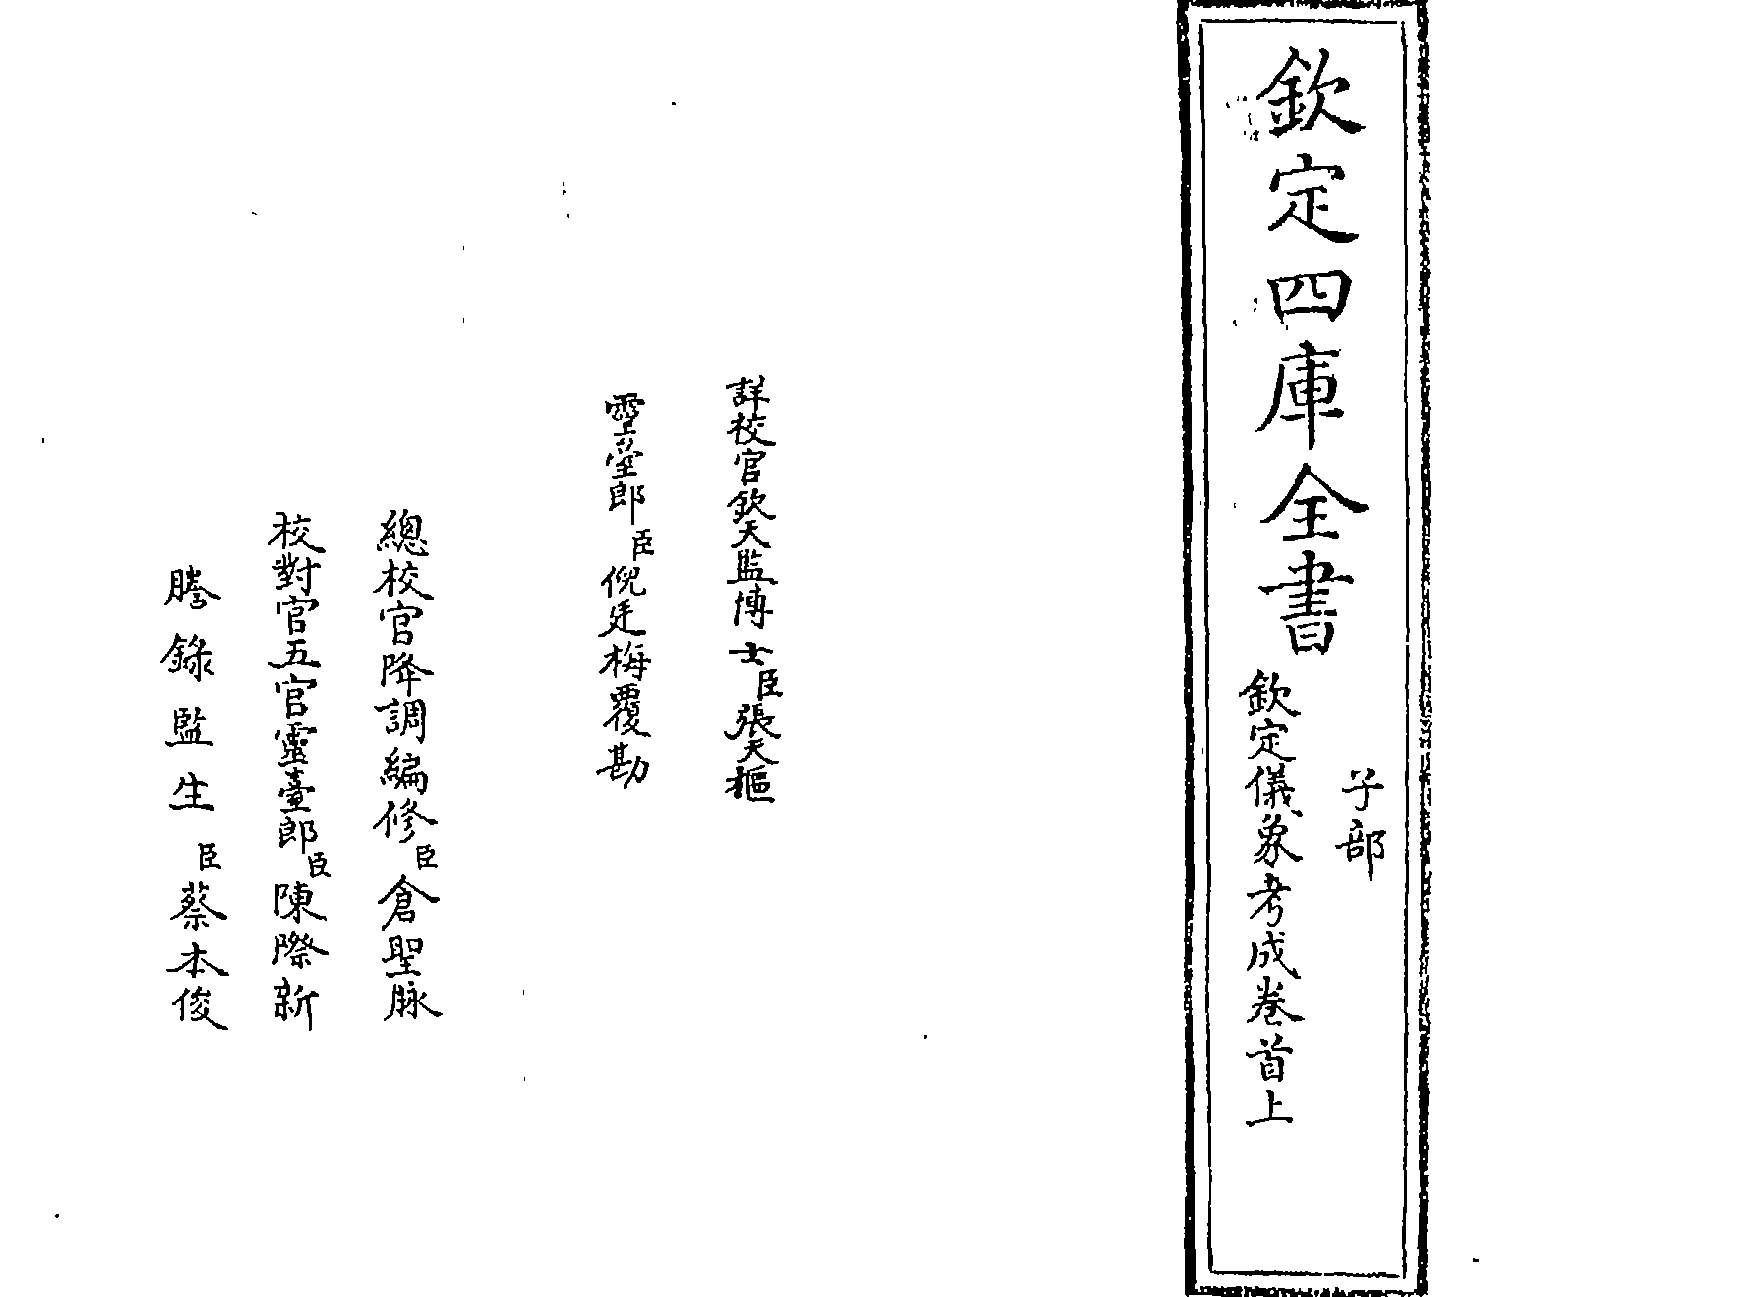
\includegraphics[width=\paperwidth,height=\paperheight,keepaspectratio]{img/0092.png}\clearpage
\begin{正文}
% ---- 册793 葉93 ----
\SetPageNumber{1}
欽定四庫全書\换行
欽定儀象考成卷首上\换行
御製璣衡撫辰儀説卷上\换行
　　儀制\换行
　　製法\换行
\char"200B\relax\换行
\char"200B\relax\换行
\char"200B\relax\换行
\char"200B\relax\换行
\char"200B\relax\换行
\char"200B\relax\换行
\char"200B\relax\换行
\char"200B\relax\换行
\char"200B\relax\换行
\char"200B\relax\换行
\char"200B\relax
\par
% ---- 册793 葉96 ----
御製璣衡撫辰儀説卷上之一\换行
　儀制\换行
　　全儀\换行
　　子午圏\换行
　　天常赤道\换行
　　赤極經圏\换行
　　遊旋赤道\换行
　　四遊圏\换行
　　指時度表\换行
　　借弧指時度表\换行
　　指緯度表\换行
　　立表\换行
　　平行立表\换行
　　平行借弧表\换行
　　綰經度表\换行
　　綰時度表
\par
% ---- 册793 葉97 ----
　　平行線測經度表\换行
\char"200B\relax\换行
\char"200B\relax\换行
\char"200B\relax\换行
\char"200B\relax\换行
\char"200B\relax\换行
\char"200B\relax\换行
\char"200B\relax\换行
\char"200B\relax\换行
\char"200B\relax\换行
\char"200B\relax\换行
\char"200B\relax\换行
\char"200B\relax\换行
\char"200B\relax\换行
\char"200B\relax\换行
\char"200B\relax
\par
\end{正文}\clearpage
\嵌图{153.00pt}{215.88pt}{395.02pt}{576.95pt}{img/0100.png}
\begin{正文}
% ---- 册793 葉100 ----
\SetPageNumber{4}
\插图页
\char"200B\relax\换行
\char"200B\relax\换行
\char"200B\relax\换行
\char"200B\relax\换行
\char"200B\relax\换行
\char"200B\relax\换行
\char"200B\relax\换行
\char"200B\relax\换行
\恢复丝栏
　　虞書舜典在璿璣玉衡以齊七政孔穎逹疏曰璣\换行
　　衡者王者正天文之器漢世以來謂之渾天儀者\换行
　　是也馬融云渾天儀可旋轉故曰璣衡其横簫所\换行
　　以視星宿也蔡邕云衡長八尺孔徑一寸下端望\换行
　　之以視星辰盖懸璣以象天而衡望之轉璣窺衡\换行
　　以知星宿是其説也上天之體不可得知測天之\换行
　　事見於經者惟此璿璣玉衡一事而已楊子法言\换行
　　云或問渾天曰落下閎營之鮮于妄人度之耿中
\par
% ---- 册793 葉101 ----
　　丞象之幾乎幾乎莫之能違也閎與妄人武帝時\换行
　　人宣帝時司農中丞耿夀昌始鑄銅為之象史官\换行
　　施用焉江南宋元嘉年太史丞錢樂\双列{\右小列{陳氏師凱曰}\左小列{錢樂本名樂}}\换行
　　\双列{\右小列{之孔疏}\左小列{脱之字}}鑄銅作渾天儀傳於齊梁周平江陵遷於\换行
　　長安尚書蔡註曰宋錢樂鑄銅作渾天儀衡長八\换行
　　尺孔徑一寸璣徑八尺圓周二丈五尺强轉而望\换行
　　之以知日月星辰之所在即璿璣玉衡之遺法也\换行
　　厯代以來其法漸密本朝因之為儀三重其在外\换行
　　者曰六合儀平置黒單環上刻十二辰八干四隅\换行
　　在地之位以凖地面而定四方側立黒雙環背刻\换行
　　去極度數以中分天脊直跨地平使其半入地下\换行
　　而結於其子午以為天經斜倚赤單環背刻赤道\换行
　　度數以平分天腹横繞天經亦使半出地上半入\换行
　　地下而結於其卯酉以為天緯三環表裏相結不\换行
　　動其天經之環則南北二極皆為圓軸虚中而内\换行
　　向以挈三辰四遊之環以其上下四方於是可考
\par
% ---- 册793 葉104 ----
　　故曰六合次其内曰三辰儀側立黒雙環亦刻去\换行
　　極度數外貫天經之軸内挈黄赤二道其赤道則\换行
　　為赤單環外依天緯亦刻宿度而結於黒雙環之\换行
　　卯酉其黄道則為黄單環亦刻宿度而又斜倚於\换行
　　赤道之腹以交結於卯酉而半入其内以為春分\换行
　　後之日軌半出其外以為秋分後之日軌又為白\换行
　　單環以承其交使不傾墊以其日月星辰於是可\换行
　　考故曰三辰其最在内者曰四遊儀亦為黒雙環\换行
　　如三辰儀之制以貫天經之軸其環之内則兩面\换行
　　當中各施直距外指兩軸而當其要中之内面又\换行
　　為小窽以受玉衡要中之小軸使衡既得隨環東\换行
　　西運轉又可隨處南北低昻以待占𠉀者之仰窺\换行
　　焉以其東西南北無不周徧故曰四遊此其法之\换行
　　大畧也今考前史漢初落下閎造渾天儀本無黄\换行
　　道或云賈逵所加或云李淳風所加或云一行所\换行
　　加而宋錢樂之渾儀之制雖有黄道並無黄道經
\par
% ---- 册793 葉105 ----
　　圈其四遊圈亦不貫於黄極則亦未盡黄道之用\换行
　　元郭守敬作簡儀乃分渾儀而變其制别設立運\换行
　　圏以測地平經緯度而不設黄道圏盖黄道與黄\换行
　　極經圏成經緯設黄道又設經圏則圏多而不便\换行
　　於測𠉀故不用黄道而專用赤道圈明正統三年\换行
　　　鑄銅渾儀簡儀於北京即宋元遺法也我\换行
　　朝康熙八年\换行
\抬头[1]聖祖仁皇帝命監臣南懐仁新製六儀赤道黄道分為二\换行
　　器皆不用地平圏而地平象限天體諸儀則地平\换行
　　之經緯與黄赤之錯綜皆已畢具康熙五十二年\换行
　　　又\换行
\抬头[1]命監臣紀利安製地平經緯儀合地平象限二儀而為一\换行
　　　其用尤便制作之妙於斯極矣我\换行
　皇上敬\换行
天法\换行
祖齊政勤民
\par
% ---- 册793 葉108 ----
親蒞靈臺徧觀儀象以渾天制最近古而時度信宜從\换行
　　今觀其㑹通斯成鉅典於是用今之數目合古之\换行
　　型模\换行
御製璣衡撫辰儀用裨測𠉀誠唐虞之遺意昭代之新\换行
　　規也儀制三重其在外者即古之六合儀而不用\换行
　　地平圏其正立雙環為子午圏兩面皆刻周天三\换行
　　百六十度自南北極起初度至中要九十度是為\换行
　　天經斜倚單環為天常赤道圏兩面皆刻周日十\换行
　　二時以子正午正當子午雙環中空之半而結於\换行
　　其中要是為天緯其南北二極皆設圓軸軸本實\换行
　　於子午雙環中空之間而軸内向以貫内二重之\换行
　　環其下承以雲座仰面正中開雙槽以受雙環東\换行
　　面正中開雲窩以受垂球下面置十字架施螺旋\换行
　　以取平架之東西兩端各植龍柱龍口銜珠開孔\换行
　　以承天常赤道卯酉之兩軸依觀象臺測定南北\换行
　　正線将座架安定則平面之四方正又依京師北
\par
% ---- 册793 葉109 ----
　　極出地三十九度五十五分自北極而上五十度\换行
　　五分即上應天頂自南極而下五十度五分即下\换行
　　對地心而應天頂之衝於天頂施小釘懸垂線而\换行
　　垂適當地心又適切於雙環之面不即不離則上\换行
　　下正立面之四方亦正而地平已在其中故不用\换行
　　地平圏也次其内即古之三辰儀而不用黄道圏\换行
　　其貫於二極之雙環為赤極經圏兩極各設軸孔\换行
　　以受天經之軸兩面皆刻周天三百六十度結於\换行
　　赤極經圏之中要與天常赤道平運者為遊旋赤\换行
　　道圈兩面皆刻周天三百六十度與天之赤道旋\换行
　　轉相應自經圏之南極作兩象限弧以承之使不\换行
　　傾墊測得三辰之赤道經緯度則黄道經緯可推\换行
　　且黄道與赤道之相距古逺今近縱或日久有差\换行
　　而儀器無庸改制故不用黄道圏也其在内者即\换行
　　古之四遊儀貫於二極之雙環為四遊圏兩面皆\换行
　　刻三百六十度定於遊圏之兩極者為直距綰於
\par
% ---- 册793 葉112 ----
　　直距之中心者為窺衡遊圏中要設直表以指經\换行
　　度及時窺衡右旁設直表以指緯度此古今所同\换行
　　無容置議者也是故體制倣乎渾天之舊而時度\换行
　　尤為整齊運量同於赤道新儀而重環更能合應\换行
　　至於借表窺測則上下左右無不宜焉夫羲和遺\换行
　　制不可考已漢世以來或作而不傳或傳而不久\换行
　　盖制器尚象若斯之難也而稽古宜今至我\换行
　朝乃臻盡善易繫傳云備物致用立成器以為天下\换行
　　利莫大乎聖人詎不信乎\换行
\char"200B\relax\换行
\char"200B\relax\换行
\char"200B\relax\换行
\char"200B\relax\换行
\char"200B\relax\换行
\char"200B\relax\换行
\char"200B\relax
\par
\end{正文}\clearpage
\嵌图{154.79pt}{220.57pt}{393.23pt}{572.26pt}{img/0118.png}
\begin{正文}
% ---- 册793 葉118 ----
\SetPageNumber{11}
\插图页
\char"200B\relax\换行
\char"200B\relax\换行
\char"200B\relax\换行
\char"200B\relax\换行
\char"200B\relax\换行
\char"200B\relax\换行
\char"200B\relax\换行
\char"200B\relax\换行
\恢复丝栏
子午圈所以正南北也天之南北定於兩極必先測定\换行
南北正線而後安置子午圈則子午圈即為南北之正\换行
線南北正而後日軌之髙下時刻之早晚中星之偏度\换行
可得而稽也其制雙環外徑六尺三寸内徑五尺六寸\换行
六分環面濶三寸二分厚九分中空一寸雙環之間四\换行
隅各施銅枕合而固之其中空之半為子午正線兩面\换行
各畫三百六十度每度六十分自南北極起初度至中\换行
要九十度古曰天經環西法舊曰緯圈盖織絲以直者
\par
% ---- 册793 葉122 ----
為經横者為緯古以其圈直立故曰經西法以其為横\换行
線所界之度故曰緯今按圈直而度横則其圈宜曰經\换行
圈而其度乃為緯度周禮賈公彦疏所謂南北之道謂\换行
之經元儒陳氏師凱所謂自北數向南去如機上數緯\换行
絲是也自兩極起初度者北極出地南極入地其度數\换行
皆自兩極起算也中要九十度者赤道為帯天之紘距\换行
兩極各一象限也南北極各設鋼軸軸本扁方長三寸\换行
濶二寸二分厚一寸實於隻環之間以鋼螺旋結之軸\换行
長六寸徑八分正當雙環中空之半内向以貫三辰四\换行
遊之環所以象天樞也\换行
\char"200B\relax\换行
\char"200B\relax\换行
\char"200B\relax\换行
\char"200B\relax\换行
\char"200B\relax\换行
\char"200B\relax
\par
\end{正文}\clearpage
\嵌图{148.32pt}{219.14pt}{399.70pt}{573.69pt}{img/0126.png}
\begin{正文}
% ---- 册793 葉126 ----
\SetPageNumber{13}
\插图页
\char"200B\relax\换行
\char"200B\relax\换行
\char"200B\relax\换行
\char"200B\relax\换行
\char"200B\relax\换行
\char"200B\relax\换行
\char"200B\relax\换行
\char"200B\relax\换行
\恢复丝栏
天常赤道所以正時刻也天左旋一日一周南北極持\换行
其兩端而赤道為其横帯以其常定不動故曰天常日\换行
循黄道右旋而其隨天西轉則係赤道之度日行臨於\换行
赤道之某位即為某時故時刻由赤道而正也其制單\换行
環外徑六尺一寸二分内徑五尺六寸四分環面濶二\换行
寸四分厚一寸四分平分其厚為赤道之中線兩面各\换行
畫周日十二時每時初正各四刻每刻十五分每一時\换行
當天之三十度每四刻當天之十五度每一分當天之
\par
% ---- 册793 葉130 ----
十五分以其子正午正線當子午雙環中空之半而結\换行
於其中要使其赤道中線適當子午圏之九十度兩圈\换行
相結成十字直角古曰天緯環西法舊曰赤道經圈盖\换行
古以其圈横運故曰緯西法以其為直線所界之度故\换行
曰經今按圈横而度直則其圈宜曰緯圈而其度乃為\换行
經度周禮賈公彦疏所謂東西之道謂之緯陳氏師凱\换行
所謂自東數向西去如機上數經絲是也上面午正時\换行
刻線結於子午圈之正北卯正居西酉正居東謂日影\换行
對照之時下面則子正居北午正居南卯正居東酉正\换行
居西為日行所臨之正位也\换行
\char"200B\relax\换行
\char"200B\relax\换行
\char"200B\relax\换行
\char"200B\relax\换行
\char"200B\relax\换行
\char"200B\relax
\par
\end{正文}\clearpage
\嵌图{153.38pt}{219.23pt}{394.64pt}{573.60pt}{img/0134.png}
\begin{正文}
% ---- 册793 葉134 ----
\SetPageNumber{15}
\插图页
\char"200B\relax\换行
\char"200B\relax\换行
\char"200B\relax\换行
\char"200B\relax\换行
\char"200B\relax\换行
\char"200B\relax\换行
\char"200B\relax\换行
\char"200B\relax\换行
\恢复丝栏
赤極經圏所以帯赤道也亦曰過極圏制如子午雙環\换行
在内而差小外徑五尺五寸六分内徑五尺一寸二分\换行
環面濶二寸二分厚八分中空一寸二分兩面皆畫三\换行
百六十度每度六十分一面自兩極起初度至赤道九\换行
十度以應天經一面自赤道起初度至兩極九十度以\换行
應赤緯南北極各設軸孔用扁方銅長三寸濶與環面\换行
等厚與雙環中空等中心開圓孔以受天經之軸其孔\换行
徑適容軸徑使旋轉不致動摇孔之兩面各施鋼片厚
\par
% ---- 册793 葉138 ----
四分使孔徑不致磨損兩軸孔之中徑適當雙環中空\换行
之半與兩極徑線參直以鋼螺旋結之環外南北極之\换行
兩端各施扁圓鋼子厚五分與内外兩雙環之分縫等\换行
貫於天經之軸使赤極經圈之中要九十度線適與子\换行
午圈之九十度相凖則内外兩圈上下四方俱合為一\换行
線而縱横經緯自宜悉協矣\换行
\char"200B\relax\换行
\char"200B\relax\换行
\char"200B\relax\换行
\char"200B\relax\换行
\char"200B\relax\换行
\char"200B\relax\换行
\char"200B\relax\换行
\char"200B\relax\换行
\char"200B\relax\换行
\char"200B\relax
\par
\end{正文}\clearpage
\嵌图{157.41pt}{218.38pt}{390.61pt}{574.45pt}{img/0142.png}
\begin{正文}
% ---- 册793 葉142 ----
\SetPageNumber{17}
\插图页
\char"200B\relax\换行
\char"200B\relax\换行
\char"200B\relax\换行
\char"200B\relax\换行
\char"200B\relax\换行
\char"200B\relax\换行
\char"200B\relax\换行
\char"200B\relax\换行
\恢复丝栏
遊旋赤道所以象天之運行而紀其赤道經度也制如\换行
天常赤道在内而差小外徑五尺五寸六分内徑五尺\换行
一寸二分環面濶二寸二分厚一寸二分平分其厚為\换行
赤道之中線兩面各畫周天三百六十度上面分為十\换行
二宫每宫三十度每度六十分下面自丑宫起初度右\换行
旋三百六十度以其丑宫未宫初度之線當赤經雙環\换行
中空之半而結於其中要使其赤道中線適當經圈之\换行
九十度兩圈相結成十字直角與天之赤道旋轉相應
\par
% ---- 册793 葉146 ----
又於經圏南極之兩旁設象限弧承於遊旋赤道辰宫\换行
戌宫之下以螺旋結之使不傾墊有天常赤道之不動\换行
者以定時又有遊旋赤道之常動者以紀度則赤道之\换行
逐宫逐度皆能周行於十二時而三辰之所躔與兩曜\换行
之相距皆可得而稽矣\换行
\char"200B\relax\换行
\char"200B\relax\换行
\char"200B\relax\换行
\char"200B\relax\换行
\char"200B\relax\换行
\char"200B\relax\换行
\char"200B\relax\换行
\char"200B\relax\换行
\char"200B\relax\换行
\char"200B\relax\换行
\char"200B\relax
\par
\end{正文}\clearpage
\嵌图{152.17pt}{219.82pt}{395.85pt}{573.01pt}{img/0150.png}
\begin{正文}
% ---- 册793 葉150 ----
\SetPageNumber{19}
\插图页
\char"200B\relax\换行
\char"200B\relax\换行
\char"200B\relax\换行
\char"200B\relax\换行
\char"200B\relax\换行
\char"200B\relax\换行
\char"200B\relax\换行
\char"200B\relax\换行
\恢复丝栏
四遊圈所以測三辰之赤道經緯度也制如赤經雙環\换行
在内而差小外徑五尺内徑四尺六寸八分環面濶一\换行
寸六分厚七分中空一寸四分盖三重雙環之外面皆\换行
相平而内重則漸薄中空則漸大取其輕重適宜亦便\换行
於設窺衡也兩面各畫三百六十度一面自北極起初\换行
度至南極一百八十度為去極度一面自赤道起初度\换行
至兩極各九十度為距緯度南北極各設軸孔以受夭\换行
經之軸與過極圈同環外南北極之兩端各施扁圓鋼
\par
% ---- 册793 葉152 ----
子厚六分與赤經四遊兩環之分縫等貫於天經之軸\换行
其下半周之中要安直表以指經度及時刻兩面對南\换行
北極各安直距如圓之通徑濶一寸六分厚七分中空\换行
一寸四分直距之二面對環之兩極作直徑線對環之\换行
九十度作横徑線十字相交中心開圓孔施螺旋小鋼\换行
軸而圓其末以綰窺衡窺衡長四尺七寸二分方一寸\换行
二分中空一寸上下兩端施方銅盖厚五分内三分方\换行
一寸入於管中外二分方一寸二分齊於管面中心開\换行
圓孔上端孔心留十字線以便測視管之四面亦各取\换行
中線上面安立表下端右面安指緯度表左右兩面之\换行
中心各開圓孔使直距中要小軸之末入其中以綰之\换行
則窺衡乃能南北低昂而隨雙環東西運轉焉窺衡連\换行
盖長四尺七寸六分比四遊環内徑長八分兩端各施\换行
鋼篐厚一分中要孔外施鋼眼錢亦厚一分使其左右\换行
適切於中空之内面上下兩端入於雙環内徑各四分\换行
則上下低昂自無偏側而所測經緯度必皆密合矣
\par
\end{正文}\clearpage
\嵌图{153.29pt}{217.38pt}{394.73pt}{575.45pt}{img/0153.png}
\begin{正文}
% ---- 册793 葉153 ----
\SetPageNumber{21}
\插图页
\char"200B\relax\换行
\char"200B\relax\换行
\char"200B\relax\换行
\char"200B\relax\换行
\char"200B\relax\换行
\char"200B\relax\换行
\char"200B\relax\换行
\char"200B\relax\换行
\恢复丝栏
指時度表通長七寸三分本長一寸六分形如方筒入\换行
於四遊雙環中空之間濶一寸四分與四遊環之中空\换行
等平分其濶即當窺衡之中線筒中施左右螺旋以充\换行
塞於中空之内使表不動移横帶長三寸二分濶五分\换行
兩端各鉤囬二分扣於環面之外表長五寸二分濶一\换行
寸其指時度之邊線對方筒之正中亦即窺衡之正中\换行
下端二寸四分厚三分切於遊旋赤道之面以指度分\换行
上端二寸八分厚二分切於天常赤道之面以指時刻
\par
% ---- 册793 葉156 ----
也\换行
\char"200B\relax\换行
\char"200B\relax\换行
\char"200B\relax\换行
\char"200B\relax\换行
\char"200B\relax\换行
\char"200B\relax\换行
\char"200B\relax\换行
\char"200B\relax\换行
\char"200B\relax\换行
\char"200B\relax\换行
\char"200B\relax\换行
\char"200B\relax\换行
\char"200B\relax\换行
\char"200B\relax\换行
\char"200B\relax
\par
\end{正文}\clearpage
\嵌图{151.20pt}{217.28pt}{396.82pt}{575.55pt}{img/0157.png}
\begin{正文}
% ---- 册793 葉157 ----
\SetPageNumber{23}
\插图页
\char"200B\relax\换行
\char"200B\relax\换行
\char"200B\relax\换行
\char"200B\relax\换行
\char"200B\relax\换行
\char"200B\relax\换行
\char"200B\relax\换行
\char"200B\relax\换行
\恢复丝栏
借弧指時度表其本方筒及横帶長濶並與前指時度\换行
表同横帶之下自左向右立安弧背一道長九寸三分\换行
濶一寸二分厚一分六釐弧背之末平安指時度表除\换行
弧背之厚長五寸二分濶一寸計自表本方筒之中線\换行
至指時度表之内邊長六寸七分當遊旋赤道之十五\换行
度當天常赤道之一小時測量時指時度表或為子午\换行
圏所礙則用此表視其所指之時度加四刻即為所測\换行
之時減十五度即為所測之度盖借弧指時度表在窺
\par
% ---- 册793 葉160 ----
衡之右所指雖視乎借表而所測則定於窺衡天常之\换行
時刻左旋故加三辰之度分右旋故減則用借弧指時\换行
度表察之與用指時度表等也\换行
\char"200B\relax\换行
\char"200B\relax\换行
\char"200B\relax\换行
\char"200B\relax\换行
\char"200B\relax\换行
\char"200B\relax\换行
\char"200B\relax\换行
\char"200B\relax\换行
\char"200B\relax\换行
\char"200B\relax\换行
\char"200B\relax\换行
\char"200B\relax\换行
\char"200B\relax
\par
\end{正文}\clearpage
\嵌图{151.20pt}{220.43pt}{396.82pt}{572.40pt}{img/0161.png}
\begin{正文}
% ---- 册793 葉161 ----
\SetPageNumber{25}
\插图页
\char"200B\relax\换行
\char"200B\relax\换行
\char"200B\relax\换行
\char"200B\relax\换行
\char"200B\relax\换行
\char"200B\relax\换行
\char"200B\relax\换行
\char"200B\relax\换行
\恢复丝栏
指緯度表其形兩曲安於窺衡下端之右面底長三寸\换行
濶九分平分其濶為中線對衡面中線以螺旋結之曲\换行
横七分與四遊環之厚等又曲長一寸七分切於四遊\换行
環之外面從中線減濶之半所以指緯度也\换行
\char"200B\relax\换行
\char"200B\relax\换行
\char"200B\relax\换行
\char"200B\relax
\par
\end{正文}\clearpage
\嵌图{153.29pt}{219.54pt}{394.73pt}{573.29pt}{img/0164.png}
\begin{正文}
% ---- 册793 葉164 ----
\SetPageNumber{26}
\插图页
\char"200B\relax\换行
\char"200B\relax\换行
\char"200B\relax\换行
\char"200B\relax\换行
\char"200B\relax\换行
\char"200B\relax\换行
\char"200B\relax\换行
\char"200B\relax\换行
\恢复丝栏
立表二座形直底平表髙底長各三寸二分濶九分厚\换行
一分平分其濶為中線表直立於底長之半與底面成\换行
直角距底面一寸一表向上開長方孔長一寸中留直\换行
線又上五分開圓孔徑四分中留十字線安於窺衡之\换行
上端一表依前度下開直縫上開小圓孔安於窺衡之\换行
下端各對衡面中線以螺旋結之測量時窺衡或為赤\换行
道及銅枕所礙則用此表盖兩表之孔心中線距衡面\换行
皆相等又與衡面之中線參直則用立表測之與用窺
\par
% ---- 册793 葉165 ----
衡等也\换行
\char"200B\relax\换行
\char"200B\relax\换行
\char"200B\relax\换行
\char"200B\relax\换行
\char"200B\relax\换行
\char"200B\relax\换行
\char"200B\relax\换行
\char"200B\relax\换行
\char"200B\relax\换行
\char"200B\relax\换行
\char"200B\relax\换行
\char"200B\relax\换行
\char"200B\relax\换行
\char"200B\relax\换行
\char"200B\relax
\par
\end{正文}\clearpage
\嵌图{153.00pt}{217.70pt}{395.02pt}{575.13pt}{img/0168.png}
\begin{正文}
% ---- 册793 葉168 ----
\SetPageNumber{28}
\插图页
\char"200B\relax\换行
\char"200B\relax\换行
\char"200B\relax\换行
\char"200B\relax\换行
\char"200B\relax\换行
\char"200B\relax\换行
\char"200B\relax\换行
\char"200B\relax\换行
\恢复丝栏
平行立表二座形曲底平底盤長四寸濶一寸二分厚\换行
一分中空長三寸二分濶九分與立表底盤之長濶等\换行
表曲如勾股股直如立表髙三寸二分濶九分勾横連\换行
於股末長五寸濶九分横植於底盤之末底盤中空冒\换行
於立表底盤之外以掐表固之測量時窺衡立表或為\换行
子午圏及龍柱所礙則用此表盖平行立表曲如勾股\换行
而與立表平行則用平行立表測之與用立表等亦與\换行
用窺衡等也
\par
\end{正文}\clearpage
\嵌图{153.00pt}{223.19pt}{395.02pt}{569.64pt}{img/0169.png}
\begin{正文}
% ---- 册793 葉169 ----
\SetPageNumber{29}
\插图页
\char"200B\relax\换行
\char"200B\relax\换行
\char"200B\relax\换行
\char"200B\relax\换行
\char"200B\relax\换行
\char"200B\relax\换行
\char"200B\relax\换行
\char"200B\relax\换行
\恢复丝栏
平行借弧表制如平行立表而倒正異盖四遊窺衡東\换行
西為子午圏及龍柱所礙南北為赤道及銅枕所礙則\换行
用平行立表猶是窺衡所能及而管孔被遮故其表平\换行
行正立即可見若近北極之星則東西既礙於子午圏\换行
南北又礙於極軸窺衡不能及自上測之不能及北極\换行
之南六度餘自下測之不能及北極之北六度餘故借\换行
十度作平行借弧表一表上植一表下垂則窺衡未及\换行
北極十度而窺孔之視線已與北極參直其法以半徑
\par
% ---- 册793 葉172 ----
一千萬為一率十度之正切線一百七十六萬三千二\换行
百七十為二率表之横勾距窺衡中心二尺三寸三分\换行
為三率求得四率四寸一分零八毫為表髙之中數\双列{\右小列{自}\左小列{窺}}\换行
\双列{\右小列{衡中線至直}\左小列{距中線之數}}上端之表立植於衡面則中數即表髙\双列{\右小列{中}\左小列{數}}\换行
\双列{\右小列{減衡方之半六分加表端距窺孔中心}\左小列{六分為表端至表本之髙仍與中數等}}下端之表自衡\换行
面下垂則於中數加衡方之半六分表端距窺孔中心\换行
六分又加平行横勾之濶九分得六寸二分零八毫為\换行
表之髙距表端下六分開圓孔又下五分開長方孔皆\换行
與立表制同凡測近北極之星測得距赤道北若干加\换行
十度即得星距赤道北之緯度若測赤道南之星亦可\换行
用此表但測得距赤道南若干減十度即得星距赤道\换行
南之緯度也\换行
\char"200B\relax\换行
\char"200B\relax\换行
\char"200B\relax\换行
\char"200B\relax
\par
\end{正文}\clearpage
\嵌图{155.09pt}{220.28pt}{392.93pt}{572.55pt}{img/0173.png}
\begin{正文}
% ---- 册793 葉173 ----
\SetPageNumber{31}
\插图页
\char"200B\relax\换行
\char"200B\relax\换行
\char"200B\relax\换行
\char"200B\relax\换行
\char"200B\relax\换行
\char"200B\relax\换行
\char"200B\relax\换行
\char"200B\relax\换行
\恢复丝栏
綰經度表通長四寸濶一寸四分平分其濶即當窺衡\换行
之中線其本方筒長一寸六分髙一寸八分入於四遊\换行
雙環之間以左右螺旋固之其末上下二面以夾遊旋\换行
赤道上面濶七分減本之半與窺衡中線參直下面以\换行
螺旋固之所以綰定遊旋赤道之經度於四遊圈也\换行
\char"200B\relax\换行
\char"200B\relax\换行
\char"200B\relax
\par
\end{正文}\clearpage
\嵌图{153.29pt}{222.42pt}{394.73pt}{570.41pt}{img/0176.png}
\begin{正文}
% ---- 册793 葉176 ----
\SetPageNumber{32}
\插图页
\char"200B\relax\换行
\char"200B\relax\换行
\char"200B\relax\换行
\char"200B\relax\换行
\char"200B\relax\换行
\char"200B\relax\换行
\char"200B\relax\换行
\char"200B\relax\换行
\恢复丝栏
綰時度表内外二截内截上下内三面綰於遊旋赤道\换行
之内規上面之末承於外截之下開二方孔以受外截\换行
之方足下面以螺旋固之外截上下外三面綰於天常\换行
赤道之外規上面之末覆於内截之上安二方足入於\换行
内截之方孔下面以螺旋固之凡以太陽時刻及經度\换行
測月星則内外截俱綰定别測月星若以經度求時刻\换行
則止綰定内截外截隨之運轉視其所當刻分即得時\换行
刻若以時刻求經度則止綰定外截任遊旋赤道之運
\par
% ---- 册793 葉177 ----
轉視其所當度分即得經度也\换行
\char"200B\relax\换行
\char"200B\relax\换行
\char"200B\relax\换行
\char"200B\relax\换行
\char"200B\relax\换行
\char"200B\relax\换行
\char"200B\relax\换行
\char"200B\relax\换行
\char"200B\relax\换行
\char"200B\relax\换行
\char"200B\relax\换行
\char"200B\relax\换行
\char"200B\relax\换行
\char"200B\relax\换行
\char"200B\relax
\par
\end{正文}\clearpage
\嵌图{146.46pt}{204.81pt}{838.85pt}{580.16pt}{img/0180.png}
\begin{正文}
% ---- 册793 葉180 图版 ----
\SetPageNumber{34}
\插图页
\char"200B\relax\换行
\char"200B\relax\换行
\char"200B\relax\换行
\char"200B\relax\换行
\char"200B\relax\换行
\char"200B\relax\换行
\char"200B\relax\换行
\char"200B\relax\换行
\char"200B\relax\换行
\char"200B\relax\换行
\char"200B\relax\换行
\char"200B\relax\换行
\char"200B\relax\换行
\char"200B\relax\换行
\char"200B\relax\换行
\char"200B\relax
\恢复丝栏\par
% ---- 册793 葉181 ----
平行線測經度表以赤經之平行線與直距之平行線\换行
相參直\双列{\右小列{赤經之平行線在圓周直距之平行線在}\左小列{圓心其平行線之間俱對南北極之中徑}}而測\换行
距星之經度也其制於直距南北極之兩端各安銅板\换行
如工字形正方二寸八分與直距二面之分等\双列{\右小列{直距二}\左小列{面各厚}}\换行
\双列{\右小列{七分中空一寸四}\左小列{分共二寸八分}}兩要各缺一長方長一寸六分濶七\换行
分與直距一面之分等\双列{\右小列{直距二面每面濶}\左小列{一寸六分厚七分}}扣於直距中\换行
空之間中心開圓孔貫於天經之軸四隅距中心一寸\换行
九分\双列{\右小列{銅板方二寸八分對角斜線三寸九分八釐四隅}\左小列{距中心各一寸九分九釐今取一寸九分餘九釐}}\换行
各安立柱圓頂開孔以穿直線與直距中徑平行下安\换行
小環以為結赤經平行線之用又按距星宫度於遊旋\换行
赤道安赤經平行線表其制上畫半圓内容半方自對\换行
角斜線起初度至横徑為四十五度其中直徑與指度\换行
表之邊線參直半圓中心安二遊表各長二寸距中心\换行
一寸九分邊留小臍中開小圓孔與直距四隅立柱之\换行
距中心等以線穿之上端繫於北極銅板對角之兩環\换行
下端貫於南極銅板對角之兩環各以垂球墜之乃視
\par
% ---- 册793 葉184 ----
四遊圏之所測與此平行線之所測相距若干度即将\换行
遊表對半圓度數安定下面以螺旋中徑以壓表固之\换行
此二線必與赤經中徑平行而與直距中徑之二平行\换行
線廣狹相等從左線視之與所測參直從右線視之亦\换行
與所測參直則此二線即為距星經度之凖線以此線\换行
對定距星将遊旋赤道隨之運轉又以四遊圏及窺管\换行
測日月及星即得其經緯度也盖以一星作距測日月\换行
及星必用兩測舊制黄道赤道二儀南北極之通徑皆\换行
係圓軸故測𠉀用通光耳實其正中與軸徑等兩邊各\换行
開直縫從左縫對軸左邊見光從右縫對軸右邊見光\换行
亦猶用平行線之意也今不用圓軸而用直距兩測相\换行
距有逺近則直距對角有斜横斜則二線平距之分狹\换行
横則二線平距之分廣\双列{\右小列{直鉅銅板方分也其對角斜分}\左小列{也二線平距則横分也對角斜}}\换行
\双列{\右小列{則平距為斜之方故狹對角}\左小列{横則平距為方之斜故廣}}其限自正斜起初度至四\换行
十五度而横四十五度以後復由横而斜至九十度與\换行
初度同\双列{\右小列{九十度以後復由斜而横至一百三十五度與}\左小列{四十五度同一百三十五度以後復由横而斜}}
\par
% ---- 册793 葉185 ----
\双列{\右小列{至一百八十度與初}\左小列{度同盈半周天而止}}如四遊環與平行線表同度是為\换行
初度是時直距對角正斜而其二線平距之分為斜之\换行
方此二線平距之最狹者也過此而四遊環距平行線\换行
表漸逺則直距對角漸横而二線平距漸廣至四遊環\换行
距平行線表四十五度則直距對角正横而其二線平\换行
距之分為方之斜此二線平距之最廣者也過此則直\换行
距對角又漸斜而二線平距又漸狹至九十度正斜而\换行
最狹故又與初度同也今欲使赤經平行線與直距平\换行
行線廣狹相等必以直距對角斜横之度合於赤道之\换行
半圓遊表二線距圓心各一寸九分通共三寸八分即\换行
直距銅板對角之斜分也半圓自内方之對角斜線起\换行
初度即直距對角之初度為正斜也半圓至横徑為四\换行
十五度即直距對角之四十五度為正横也設以二遊\换行
表通為一直表則與直距對角之斜横儼為一體但遊\换行
表在赤道若通為一直表則其線為赤道所礙而廣狹\换行
不靈且通為一表此端在横徑内彼端必在横徑外凡
\par
% ---- 册793 葉188 ----
斜線與十字線過心相交其彼端距横徑外之度與此\换行
端距横徑内之度必相等而距中徑之濶亦相等故以\换行
直表彼端當横徑外之度另用一遊表於横徑内按度\换行
安之其距中徑之濶必相等而與直距二平行線廣狹\换行
亦相等則用平行線表亦猶用通光耳之意也\换行
\char"200B\relax\换行
\char"200B\relax\换行
\char"200B\relax\换行
\char"200B\relax\换行
\char"200B\relax\换行
\char"200B\relax\换行
\char"200B\relax\换行
\char"200B\relax\换行
\char"200B\relax\换行
\char"200B\relax\换行
\char"200B\relax
\par
% ---- 册793 葉189 ----
御製璣衡撫辰儀説卷上之二\换行
　製法\换行
　　銅質宜精\换行
　　型制宜工\换行
　　鏇磨宜平\换行
　　取心宜中\换行
　　輕重宜審\换行
　　界度宜均\换行
　　兩徑合度\换行
　　合結均齊\换行
　　三重同心\换行
　　安置方正\换行
\char"200B\relax\换行
\char"200B\relax\换行
\char"200B\relax\换行
\char"200B\relax
\par
% ---- 册793 葉192 ----
　　銅質宜精\换行
凡鑄黄銅器具應用紅銅六成倭鉛四成鎔錬精到然\换行
後鑄之遼厯象志云古之鍊銅黒黄白青之氣盡然後\换行
用之故可施於久逺唐一行鑄渾天儀時稱精妙理固\换行
然也\换行
　　型制宜工\换行
凡鑄儀器以土為型必先治地極平外規較定制微大\换行
内規較定制微小其外環面如輪次内如輻次内如轂\换行
中留環心務極圓平合度則所鑄之體自亦圓平而鏇\换行
磨亦易為力矣\换行
　　鏇磨宜平\换行
凡製儀器必用鏇磨圓環中心當治方孔以受軸軸圓\换行
而方其端施於環心之方孔使環之上下前後左右不\换行
得動揺則鏇之自圓且平矣\换行
　　取心宜中\换行
凡製圓器必取中心心中則界正未鏇之前環心尚在
\par
% ---- 册793 葉193 ----
圓規方孔皆自環心取中逮鏇之既成則無中心矣而\换行
畫儀器之圓線則必先取中心為凖須以直木為環徑\换行
其兩端即如環之内規切𦂳安定約其中心嵌定鐵板\换行
任於環之内規取三處作點用三點求圓心法\双列{\右小列{法見數}\左小列{理精藴}}\换行
求得圓心即於鐵板作記次以鋼製規徑一規尖二規\换行
尖之本開方孔貫於規徑之兩端一尖安於圓心一尖\换行
按環面内外規之度各用螺旋固之於環之内外規旋\换行
轉比試處處皆當規面則圓心中矣次依環之内外規\换行
取外界圓線半徑之度安定規尖畫外界圓線為度之\换行
外界即以此半徑度将外界圓線分為六觚毎觚六十\换行
度\双列{\右小列{半徑與六十}\左小列{度之通弦等}}又取内界圓線半徑之度安定規尖畫\换行
内界圓線為度之内界自外界每觚六十度之點平分\换行
之得三十度各對中心作直線抵内界其過心對角之\换行
線即圓之通徑而平分環面為兩半周則圓界正矣次\换行
将直線輕微引出外界至外規用極方正矩度凖於側\换行
面單環則自側面即凖於彼面雙環則自此環之側面
\par
% ---- 册793 葉196 ----
凖於彼環之側面復自彼環之側面凖於彼環之彼面\换行
輕微畫線作記乃用前直木環徑切𦂳安定以縱横二\换行
線對於所凖之通徑果於中心相交則所凖確合否則\换行
又用前法取心務令得中單環即可如前畫彼面之圓\换行
線及十二度線雙環則俟審定輕重合釘枕銅再行比\换行
試確凖然後可畫彼面也\换行
　　輕重宜審\换行
凡環之兩半周輕重適均則平置無偏側之失運轉無\换行
游移之弊審量之法用圓直鐵鋌徑八分\双列{\右小列{與軸}\左小列{徑等}}長逾環\换行
徑平分中線卧置之使不動移而以環面之通徑線加\换行
於其上易置試之兩半周無有低昂則輕重適均否則\换行
非其線有微差即其體質不等細察磨治務得其輕重\换行
之適均則天常赤道之子正午正遊旋赤道之丑宫未\换行
宫三雙環之南北極皆以此通徑為凖乃将雙環已畫\换行
十二度線之一面置於下以通徑凖線四象分中安設\换行
銅枕以雙環彼面之通徑凖線合於上釘而固之復用
\par
% ---- 册793 葉197 ----
前法比試確凖取定中心然後畫内外界圓線及十二\换行
度線則兩面之圓心圓界允協矣\换行
　　界度宜均\换行
環心既中環界既正則界度可得而均矣顧諸環皆取\换行
度分惟天常赤道取時刻然時刻亦與度分相凖故取\换行
度分者将每觚六十度平分之得三十度又三分之各\换行
為十度自外界抵内界各畫直線而於内界之外畫圓\换行
線一層是為十度界次将每十度又十分之各為一度\换行
自外界抵十度界各畫直線而於十度界之外外界之\换行
内各畫圓線一層是為度界次於内度界之外外度界\换行
之内各畫圓線一層為十分界将每度六分之各為十\换行
分畫直線於其界内次於内外兩十分界之間畫圓線\换行
九道界為十層自每十分之初至每十分之末各作對\换行
角斜線則每一圓線與斜線之交即逐度之一分也取\换行
時刻者每三十度為一時平分之得十五度為一小時\换行
每一小時分為四刻自外界抵内界各畫直線而於内
\par
% ---- 册793 葉200 ----
界之外畫圓線一層是為時刻界次将每刻十五分三\换行
分之各為五分自外界抵時刻界各畫直線而於時刻\换行
界之外外界之内各畫圓線一層是為五分界次於内\换行
五分界之外外五分界之内又各畫圓線一層為一分\换行
界而将每五分又各五分之各為一分畫直線與其界\换行
内次於内外兩一分界之間畫圓線十一道界為十二\换行
層自每一分之初至每一分之末作對角斜線則每一\换行
圓線與斜線之交即逐分之五秒也\双列{\右小列{每分為六十秒十}\左小列{二分之故為五秒}}\换行
　　兩徑合度\换行
界度既均儀體正矣而其用尤在於軸稍滯則運轉不\换行
靈稍滑則游移不定是必軸身與軸孔兩徑相同密相\换行
合切而後無滯滑之失其法以極精鋼製成軸本軸身\换行
近本徑八分近末微細以銅製為軸孔\双列{\右小列{軸本軸孔皆扁}\左小列{方體詳前儀制}}\换行
\双列{\右小列{本}\左小列{篇}}上下孔面各嵌鋼片厚五分開成圓孔較軸身微小\换行
乃以油濡軸身轉而入之鋼屑如泥隨轉而出軸外孔\换行
内更不容間則以軸身治軸孔即以軸孔治軸身故兩
\par
% ---- 册793 葉201 ----
徑密相合切而自無滯滑之弊也\换行
　　合結均齊\换行
經緯各環製造既已如式而合結尤宜均齊其法先将\换行
子午圏之軸本過極圏四遊圏之軸孔三扁方治令方\换行
正十字分中\双列{\右小列{凡圏皆正立軸本軸孔入於雙環之間軸}\左小列{本扁方先将東西二面及南北兩端各對}}\换行
\双列{\右小列{軸徑取中線次将上面作十字線軸孔扁方先将上下}\左小列{二面各對軸孔作十字線次将東西二面南北兩端取}}\换行
\双列{\右小列{中}\左小列{線}}自中線各取雙環中空之半為其扁方之厚\双列{\右小列{子午圏}\左小列{中空一}}\换行
\双列{\右小列{寸過極圏中空一寸二分}\左小列{四遊圏中空一寸四分}}入於雙環中空之間\双列{\右小列{扁方微}\左小列{厚則不}}\换行
\双列{\右小列{動}\左小列{}}次於軸本軸孔之中心結通徑線\双列{\右小列{上下二軸各安銅}\左小列{管其端之中心開}}\换行
\双列{\右小列{小圓孔以線結之上下二孔各安}\左小列{銅片其中心開小圓孔以線結之}}雙環之中空二極之\换行
兩面各結十字線\双列{\右小列{雙環中空上下對扁方十字直線中}\左小列{間對銅枕厚分之半以線圍而結之}}\换行
\双列{\右小列{二極上下對扁方十字横線内}\左小列{面對極中徑以線圍而結之}}三線相參\双列{\右小列{通徑直線一}\左小列{十字圍線二}}\换行
\双列{\右小列{縱横}\左小列{皆三}}倘一線有毫釐之差則非中心有偏即十字線不\换行
正中心有偏者治扁方十字不正者治直線務令三線\换行
相合始為得中即於上下二扁方及四銅枕刻線作記\换行
以為合結之用乃将軸本軸孔之扁方二極雙環之兩
\par
% ---- 册793 葉204 ----
面皆自中線取分各作四孔以銅螺旋結之\夹注[only-column=right, auto-balance=false, grid-height=22.35pt, font-size=19.16pt]{徑三分試定}\夹注[only-column=left, auto-balance=false, grid-height=22.35pt, font-size=19.16pt]{易鋼螺旋徑}\换行
\抬头[1]\双列{\右小列{四}\左小列{分}}次將過極圏與遊旋赤道合結為三辰儀於過極雙環\换行
\抬头[1]之南北兩半周去極九十度中線之上下各取六分與九\换行
\抬头[1]十度作平行線自内規面向外各取一寸一分與南北極\换行
\抬头[1]作平行線依線裁成缺口以受赤道之内入又於遊旋赤\换行
\抬头[1]道之南北兩半周丑宮未宮之東或西取一寸四分與冬\换行
\抬头[1]夏至作平行線\双列{\右小列{作線於東則半弧背自西裁作線}\左小列{於西則半弧背自東裁法理皆同}}自外規\换行
\抬头[1]面向内各取一寸一分與辰宮戌宮作平行線依線裁去\换行
\抬头[1]半弧背\双列{\右小列{凡裁弧皆梢留有餘}\左小列{比試合切使令方正}}以足過極圏之内容則遊旋\换行
\抬头[1]赤道適容入於過極雙環之内而丑宮未宮線適當雙環\换行
中空之間\夹注[only-column=right, auto-balance=false, grid-height=23.75pt, font-size=20.36pt]{遊旋赤道外徑五尺五寸六分南北各裁一寸一分}\夹注[only-column=left, auto-balance=false, grid-height=23.75pt, font-size=20.36pt]{餘五尺三寸四分過極圏内徑五尺一寸二分}\换行
\夹注[only-column=right, auto-balance=false, grid-height=26.68pt, font-size=22.87pt]{南北各開一寸一分亦得五尺三寸四分九十度中線之}\夹注[only-column=left, auto-balance=false, grid-height=26.68pt, font-size=22.87pt]{上下各去六分共去一寸二分與遊旋赤道之厚等丑宮}\换行
\夹注[only-column=right, auto-balance=false, grid-height=26.68pt, font-size=22.87pt]{未宮之東或西去一寸四分為雙環厚分之半故遊旋赤}\夹注[only-column=left, auto-balance=false, grid-height=26.68pt, font-size=22.87pt]{道適容入於過極雙環之内而丑宮未宮線正當雙環中}\换行
\抬头[1]\双列{\右小列{空之}\左小列{間}}乃依裁去弧背之度除雙環分位另製弧背銅補全\换行
遊旋赤道\双列{\右小列{以銅釘}\左小列{固之}}並補畵度分仍将補銅拆去合結兩\换行
環使丑宮未宮正與所記中線相對又依前法於軸孔
\par
% ---- 册793 葉205 ----
結通徑線又自雙環上下扁方直線過丑宫未宫自扁\换行
方横線過辰宫戌宫結十字線三線相參合為一線復\换行
用半徑之斜度作尺製斜尖二管貫於尺之兩端斜度\换行
之一尖直指於南北極之外界一尖直指於辰宫戌宫\换行
之外界以螺旋固之轉相比試四象限皆相符合乃将\换行
補銅釘而固之又以遊旋赤道結於過極圏之兩要恐\换行
東西兩半周日久傾墊故製二象限弧以承其下其方\换行
一寸其弧即用過極圏一象限弧之度一端減雙環厚\换行
分之半一寸四分抵於過極圏南極之外面一端減赤\换行
道厚分之半六分承於遊旋赤道辰宫戌宫之下面外\换行
加二足各長一寸二分與環面之濶等以螺旋結之復\换行
以前尺斜度之兩象限仍相符合\双列{\右小列{南極有二弧不可量}\左小列{故惟量北極兩象限}}\换行
\双列{\右小列{此兩象限合則彼}\左小列{兩象限亦必合矣}}則遊旋赤道與過極圏相交成直角\换行
均齊方正而無有偏側矣次於三辰儀之外将子午圏\换行
與天常赤道合結為六合儀其子午雙環之南北兩半\换行
周去極九十度中線之上下裁成缺口天常赤道之南
\par
% ---- 册793 葉208 ----
北兩半周裁去半弧背並另製弧背銅補畫時刻皆與\换行
三辰儀同\双列{\右小列{子午圏内規面裁去一寸二分九十度上下}\左小列{各裁七分乃能容天常赤道數雖小異而其}}\换行
\双列{\右小列{理其法}\左小列{則同也}}乃立置天常赤道圏\双列{\右小列{中線左右以木承之}\左小列{使其下可結十字線}}以裁\换行
去半弧背之半周仰於上納入三辰儀\双列{\右小列{天常赤道順列}\左小列{之十二時與遊}}\换行
\双列{\右小列{旋赤道之十二宫同在一}\左小列{面乃向北極之上面也}}将子午圏合結於其外以木\换行
橙承其四隅使二環之面相平二極之線參直周圍之\换行
分縫皆相等天常遊旋二赤道下半周之分縫以木片\换行
實之使周圍亦相等乃将軸本入於子午圏南北極中\换行
空之間貫於過極圈南北極之軸孔使扁方之四孔與\换行
環面之四孔相合以銅螺旋結之依前法於軸端結通\换行
徑線子午卯酉各結十字線三線相參合為一線又用\换行
斜尺絜度四象限皆相符合乃将補銅釘而固之則子\换行
午圏與天常赤道相交成直角均齊方正無有偏側又\换行
卯正酉正有二小軸承於龍柱之珠孔自不虞傾墊矣\换行
至於四遊圏與窺衡合結為四遊儀其法較易已詳儀\换行
制並見後篇
\par
% ---- 册793 葉209 ----
　　三重同心\换行
前篇分言合結之法先正其樞心次正其經緯宜其無\换行
不正矣然三重合為一儀必三重同心施之測量乃得\换行
允協且以一重而言三線相參視之猶逺二線相切即\换行
有一線之差再以二重合之尤易參錯則先合定外二\换行
重比較確凖而後加入内一重其中正較為易得也盖\换行
子午圏過極圏貫於一軸則子午圈之軸本即天常赤\换行
道之中心過極圏之軸孔即遊旋赤道之中心如兩心\换行
皆得其中則兩心合而為一遊旋赤道之宫度線必與\换行
天常赤道之時刻線相合如一心有偏則兩心岐而為\换行
二而宫度線與時刻線不合矣然有偏東西與偏南北\换行
之殊又有軸本偏與軸孔偏之異偏東西者軸本軸孔\换行
厚分之中線不正當中空之半或偏東或偏西故丑宫\换行
未宫線亦偏子正午正之或東或西也偏南北者軸本\换行
軸孔扁方之中線不正當環面之徑或偏北或偏南故\换行
辰宫戌宫線亦偏卯正酉正之或北或南也治之之法
\par
% ---- 册793 葉212 ----
先正東西立置子午圏按方位安定北極在上南極在\换行
下午正在北子正在南卯正在西酉正在東\双列{\右小列{假如先是}\左小列{立置天常}}\换行
\双列{\右小列{赤道圏西面午正在北子正在南卯正在下酉正在上}\左小列{則子午圏西首為北極東首為南極乃以氊鋪地将天}}\换行
\双列{\右小列{常赤道圏向南推轉至子午圏在下即将子午圏東首}\左小列{轉北西首轉南向北推轉使北極在上則按位安定矣}}\换行
設以丑宫對於午正而未宫即對於子正轉以未宫對\换行
於午正而丑宫亦對於子正則東西正一有不對則東\换行
西偏比試兩次而軸本軸孔之偏正乃得而見焉凡兩\换行
試俱偏東俱偏西而偏分相等者為軸孔正軸本偏\双列{\右小列{軸}\左小列{孔}}\换行
\双列{\右小列{正則丑宫未宮線正當軸孔中心軸本偏東則挈之而}\左小列{東軸本偏西則挈之而西故所偏同向而偏分相等也}}\换行
東為軸本偏東西為軸本偏西其偏為偏分之一半\双列{\右小列{所}\左小列{謂}}\换行
\双列{\右小列{偏分者乃丑宫對午正未宫偏子正東西斜線之偏軸}\左小列{本軸孔所偏者乃丑宫未宮與子正午正平行線之偏}}\换行
\双列{\右小列{如丑宫對於午正未宫偏子正東二分若以丑宫未宫}\左小列{線與子正午正線平行則丑宫偏午正東一分未宫亦}}\换行
\双列{\右小列{偏子正東一分故其}\左小列{偏為偏分之一半}}其度之一分為尺之八毫\双列{\右小列{凡偏分}\左小列{皆以遊}}\换行
\双列{\右小列{旋赤道之度分而言遊旋赤道外徑五尺五寸六分周}\左小列{一丈七尺四寸六分七釐有竒以周天三百六十度每}}\换行
\双列{\右小列{度六十分除之得每分}\左小列{為八毫零八忽有竒}}偏東二分者為軸本偏東一分\换行
應向西移一分将上下軸本二扁方之東西記定\双列{\右小列{凡記}\左小列{方向}}
\par
% ---- 册793 葉213 ----
\双列{\右小列{只記一}\左小列{字可定}}西面去八毫東面加八毫\双列{\右小列{以薄銅}\左小列{葉釘之}}則軸本正而\换行
不偏矣偏西者凖此\双列{\右小列{凡治軸本軸孔應移八毫者上下}\左小列{各移八毫合之用線比較如上正}}\换行
\双列{\右小列{下偏則上之扁方不動下之扁方移一釐六毫如上亦}\左小列{微偏則上移四毫下移一釐二毫或上移六毫下移一}}\换行
\双列{\右小列{釐總使上下共移一釐六毫而其十字中心正}\左小列{移八毫上偏下正及偏南偏北者皆倣此治之}}凡兩試\换行
一偏東一偏西而偏分相等者為軸本正軸孔偏\双列{\右小列{軸本}\左小列{正則}}\换行
\双列{\右小列{子正午正線正當軸本中心設軸孔偏於戌宫之一面}\左小列{丑宫在北戌宫在西是軸孔偏於丑宫未宫線之西挈}}\换行
\双列{\右小列{之於軸本則丑宫未宫線必偏於子正午正線之東轉}\左小列{而丑宫在南戌宫在東是軸孔偏於丑宫未宫線之東}}\换行
\双列{\右小列{挈之於軸本則丑宫未宫線必偏於子正午}\左小列{正線之西故所偏異向而偏分亦相等也}}東為軸孔\换行
偏西西為軸孔偏東其偏亦為偏分之一半偏東二分\换行
者為軸孔偏西一分應向東移一分将上下軸孔二扁\换行
方及環面之東西記定\双列{\右小列{子午圏有定向故不須記}\左小列{過極圏有轉易故并記之}}東面\换行
去八毫西面加八毫則軸孔正而不偏矣偏西者凖此\换行
凡兩試俱偏東俱偏西而偏分不等者為軸本偏軸孔\换行
亦偏偏東分多為軸孔偏西偏西分多為軸孔偏東\双列{\右小列{軸}\左小列{本}}\换行
\双列{\右小列{偏東而軸孔又偏西挈之於軸本則丑宫未宫線必益}\左小列{在子正午正線之東故偏東分多也軸本偏西而軸孔}}\换行
\双列{\右小列{又偏東挈之於軸本則丑宫未宫線必}\左小列{益在子平午正線之西故偏西分多也}}其軸孔之偏為
\par
% ---- 册793 葉216 ----
偏多一半之半偏東多二分者為軸孔偏西半分偏西\换行
多二分者為軸孔偏東半分先治軸孔則偏分等\双列{\右小列{平行}\左小列{線之}}\换行
\双列{\右小列{偏既為偏分之一半而軸本軸孔在偏多之偏又為平}\左小列{行線所偏之一半故為一半之半如丑宫對於午正未}}\换行
\双列{\右小列{宫偏子正東二分未宫對於午正丑宫偏子正東四分}\左小列{是未宫在北偏東多二分若以丑宫未宫線與子正午}}\换行
\双列{\右小列{正線平行丑宫偏午正東一分則未宫亦偏子正東一}\左小列{分未宫偏午正東二分則丑宫亦偏子正東二分是未}}\换行
\双列{\右小列{宫在北偏東僅多一分均分其半将軸孔向東移半分}\左小列{則未宫在北丑宫未宫線偏子正午正東一分半丑宫}}\换行
\双列{\右小列{在北未宫在南丑宫未宫線亦偏子正午正東一分半}\左小列{試以丑宫對於午正則未宫偏子正東三分轉以未宮}}\换行
\双列{\右小列{對於午正丑宫亦偏子}\左小列{正東三分其偏分等}}東為軸本偏東西為軸本偏西\换行
其偏為偏分之一半再治軸本則不偏矣凡兩試一偏\换行
東一偏西而偏分不等者為軸孔偏軸本亦偏偏東分\换行
多為軸本偏東偏西分多為軸本偏西其軸本之偏亦\换行
為偏多一半之半偏東多二分者為軸本偏東半分偏\换行
西多二分者為軸本偏西半分先治軸本則偏分等\双列{\右小列{如}\左小列{丑}}\换行
\双列{\右小列{宫對於午正未宫偏子正東二分未宫對於午正丑宫}\左小列{偏子正西四分是未宫在北偏西多二分若以丑宫未}}\换行
\双列{\右小列{宫線與子正午正線平行丑宫偏午正東一分則未宫}\左小列{亦偏子正東一分未宫偏午正西二分則丑宫亦偏子}}\换行
\双列{\右小列{正西二分是未宫在北偏西僅多一分均分其半将軸}\左小列{本向東移半分則未宫在北丑宫未宫線偏子正午正}}
\par
% ---- 册793 葉217 ----
\双列{\右小列{西一分半丑宫在北未宫在南丑宫未宫線偏子正午}\左小列{正東亦一分半試以丑宫對於午正則未宫偏子正東}}\换行
\双列{\右小列{三分轉以未宫對於午正則丑}\左小列{宫偏子正西三分其偏分等}}東為軸孔偏西西為軸\换行
孔偏東其偏為偏分之一半再治軸孔則不偏矣凡兩\换行
試一正一偏者為軸本與軸孔之偏分相等一正一偏\换行
東者為軸本偏東軸孔偏西一正一偏西者為軸本偏\换行
西軸孔偏東其偏各為偏分一半之半\双列{\右小列{軸本偏東則子}\左小列{正午正線在軸}}\换行
\双列{\右小列{本之西若軸孔亦偏東其偏分等則丑宫未宫線必與}\左小列{子正午正線相合及其轉而之西則軸孔為偏西而丑}}\换行
\双列{\右小列{宫未宫線在軸孔之東挈之於軸本盖在子正午正線}\左小列{之東其偏必倍故半之為相等之偏又半之為平行線}}\换行
\双列{\右小列{之偏軸本偏}\左小列{西者凖此}}先治軸孔則變為俱偏東俱偏西其偏分\换行
等再治軸本則不偏矣若先治軸本則變為一偏東一\换行
偏西其偏分亦等再治軸孔則亦不偏矣以上凡治軸\换行
本軸孔之偏東偏西先并環面之東西記定平置子午\换行
圏用木橙承穏解螺旋下之磨治合度復結螺旋立置\换行
比試皆合則東西正其南北亦正者則辰宫戌宫與卯\换行
正酉正合為一線其南北不正者辰宫戌宫線亦必與\换行
卯正酉正線平行乃察其南北依前法以丑宫對於午
\par
% ---- 册793 葉220 ----
正未宫對於子正察辰宫戌宫線偏卯正酉正南北幾\换行
分轉以未宫對於午正丑宫對於子正察辰宫戌宫線\换行
偏卯正酉正南北幾分如此比試兩次則軸本軸孔之\换行
偏南偏北亦可得而見焉凡兩試俱偏南俱偏北而偏\换行
分相等者為軸本正軸孔偏南為軸本偏南北為軸夲\换行
偏北\双列{\右小列{皆與前法同理但}\左小列{易東西為南北耳}}偏南一分者為軸本偏南一分\换行
\双列{\右小列{辰宫戌宫線既與卯正酉正線}\左小列{平行故其偏分即為軸本之偏}}應向北移一分将上下\换行
軸本二扁方之南北記定環面四小孔向北開八毫軸\换行
夲扁方四小孔向南開八毫治令圓正易螺旋結之\双列{\右小列{環}\左小列{面}}\换行
\双列{\右小列{四小孔向北開八毫軸夲固可向北移矣然孔不圓正}\左小列{故将軸夲扁方四小孔向南開八毫治令圓正其徑較}}\换行
\双列{\右小列{大故易微大之銅螺旋結之至}\左小列{比試確凖乃易用鋼螺旋也}}則軸夲正而不偏矣偏\换行
北者凖此凡兩試一偏南一偏北而偏分相等者為軸\换行
本正軸孔偏偏南一分者為軸孔偏北一分應向南移\换行
一分将上下軸孔二扁方及環面之南北記定環面四\换行
小孔向南開八毫軸孔扁方四小孔向北開八毫治令\换行
圓正易螺旋結之則軸孔正而不偏矣偏北者凖此凡
\par
% ---- 册793 葉221 ----
兩試俱偏南俱偏北而偏分不等者為軸本偏軸孔亦\换行
偏偏南分多為軸孔偏北偏北分多為軸孔偏南其軸\换行
孔之偏為偏多之一半偏南多二分者為軸孔偏北一\换行
分偏北多二分者為軸孔偏南一分先治軸孔則偏分\换行
等\双列{\右小列{辰宫戌宫線既與卯正酉正線平行則軸本軸孔在}\左小列{偏多之偏止為平行線所偏之一半如丑宫對於午}}\换行
\双列{\右小列{正辰宫戌宫線偏卯正酉正南二分轉以未宫對於午}\左小列{正辰宫戌宫線偏卯正酉正南四分未宫在北偏南多}}\换行
\双列{\右小列{二分是軸孔偏於未宫一分将軸孔向丑宫移一分則}\左小列{丑宫在北辰宫戌宫線偏卯正酉正南三分未宫在北}}\换行
\双列{\右小列{辰宫戌宫線偏卯正酉}\左小列{正南亦三分其偏分等}}南為軸本偏南北為軸本偏北\换行
其偏即偏分再治軸本則不偏矣凡兩試一偏南一偏\换行
北而偏分不等者為軸孔偏軸本亦偏偏南分多為軸\换行
本偏南偏北分多為軸本偏北其軸本之偏亦為偏多\换行
之一半偏南多二分者為軸本偏南一分偏北多二分\换行
者為軸本偏北一分先治軸本則偏分等南為軸孔偏\换行
北北為軸孔偏南其偏即偏分再治軸孔則不偏矣凡\换行
兩試一正一偏者為軸本與軸孔之偏分相等一正一\换行
偏南者為軸本偏南軸孔偏北一正一偏北者為軸本
\par
% ---- 册793 葉224 ----
偏北軸孔偏南其偏各為偏分之一半先治軸孔則變\换行
為俱偏北俱偏南其偏分等再治軸本則不偏矣若先\换行
治軸本則變為一偏北一偏南其偏分亦等再治軸孔\换行
則亦不偏矣以上凡治軸本軸孔之偏北偏南若與偏\换行
東偏西一同比試然後解螺旋下之按分磨治未嘗不\换行
可但所偏之向或有互異易致混淆且未正東西必以\换行
丑宫未宫線與子正午正線平行方可察其偏南北而\换行
察平行線之偏兩端察視較偏子正一端之察視為難\换行
故以先正東西而後正南北之為便也六合三辰二重\换行
東西南北既正乃平置子午圏解螺旋下之加入四遊\换行
儀貫於軸本結螺旋立置如前比試則止有軸孔之偏\换行
而無軸本之偏以四遊圏南北極之中線與軸本參直\换行
則軸孔之南北正線偏南将軸孔向南移線偏北将軸\换行
孔向北移以窺衡之中線與丑宫未宫子正午正線展\换行
轉相對則軸孔之東西正線偏東将軸孔窺衡向東移\换行
線偏西将軸孔窺衡向西移\双列{\右小列{窺管中線原應與軸孔參}\左小列{直但毫釐之差甚為難辨}}
\par
% ---- 册793 葉225 ----
\双列{\右小列{且窺衡之在直距亦應東西適中如窺衡既已適中則}\左小列{移軸孔如有微偏則移窺衡窺衡東西二面各有眼錢}}\换行
\双列{\右小列{如移向東則将東面眼錢易薄西面眼錢易厚如移向}\左小列{西則西面易薄東面易厚總期窺衡中線與子正午正}}\换行
\双列{\右小列{丑宫未宫}\左小列{線相合}}如此則三重合為一心東西南北皆合為一\换行
線用以測量而經緯乃無不協也\换行
　　安置方正\换行
前言製造之法亦畧備矣然安置不正則亦不可用其\换行
法先於臺面儀基之正中取南北真線\双列{\右小列{南北真線隨地}\左小列{不同京師偏指}}\换行
\双列{\右小列{南鍼西二}\左小列{度三十分}}南北中三處各作垂線與之參直依此儀基\换行
作南北線又作十字東西線将儀座縱横對凖安定自\换行
三垂線視之與座面中線參直用三角中垂線表\双列{\右小列{木板}\左小列{為之}}\换行
\双列{\右小列{制如並矩底長六尺中長三尺兩弦各長四尺二寸四}\左小列{分平分底線為底之中自底線之兩端取弦分相交於}}\换行
\双列{\右小列{上尖為角之中自角中至底中作}\左小列{垂線為中垂線中垂線直則底平}}仰置座面以取平中\换行
心安雲座兩端安龍柱懸垂線以取直座面有兩槽以\换行
受子午雙環柱端龍口銜珠半珠開孔以受天常赤道\换行
兩傍之小軸自珠孔中心至座面槽底與子午雙環半\换行
徑等兩珠孔相距與天常赤道全徑等用三角中垂線
\par
% ---- 册793 葉228 ----
表覆於珠孔\双列{\右小列{表底兩端留小圓軸扣}\左小列{於珠孔自底中掛垂線}}表之垂線適當於\换行
雲座面之正中則雲座正而珠孔平兩珠孔之距儀心\换行
各為天常赤道全徑之一半自三垂線視之與兩槽中\换行
線參直則雲座與龍柱皆正矣乃懸全儀安置其上以\换行
北極上五十度五分為天頂南極下五十度五分為天\换行
頂之衝於子午圏之東面作上下直線對於雲座南北\换行
正中之線口\双列{\右小列{雲座東面南北正中有線}\左小列{口其下有雲窩以受垂球}}自天頂施小釘\换行
掛垂線適合上下直線而垂球入於雲窩又適切環面\换行
不即不離自三垂線視之適當子午雙環中空之半則\换行
南北東西皆正𠉀日月星至子午線用窺衡察視經緯\换行
悉協夫然後上下四方均齊方正惟用所適無不宜矣\换行
\char"200B\relax\换行
\char"200B\relax\换行
\char"200B\relax\换行
\char"200B\relax\换行
欽定儀象考成卷首上
\par

\par\end{正文}\clearpage

  % ======== 卷首下（9行20字）========
\chapter*{欽定儀象考成卷首下}
\begin{正文}
\end{正文}\clearpage
\thispagestyle{empty}\noindent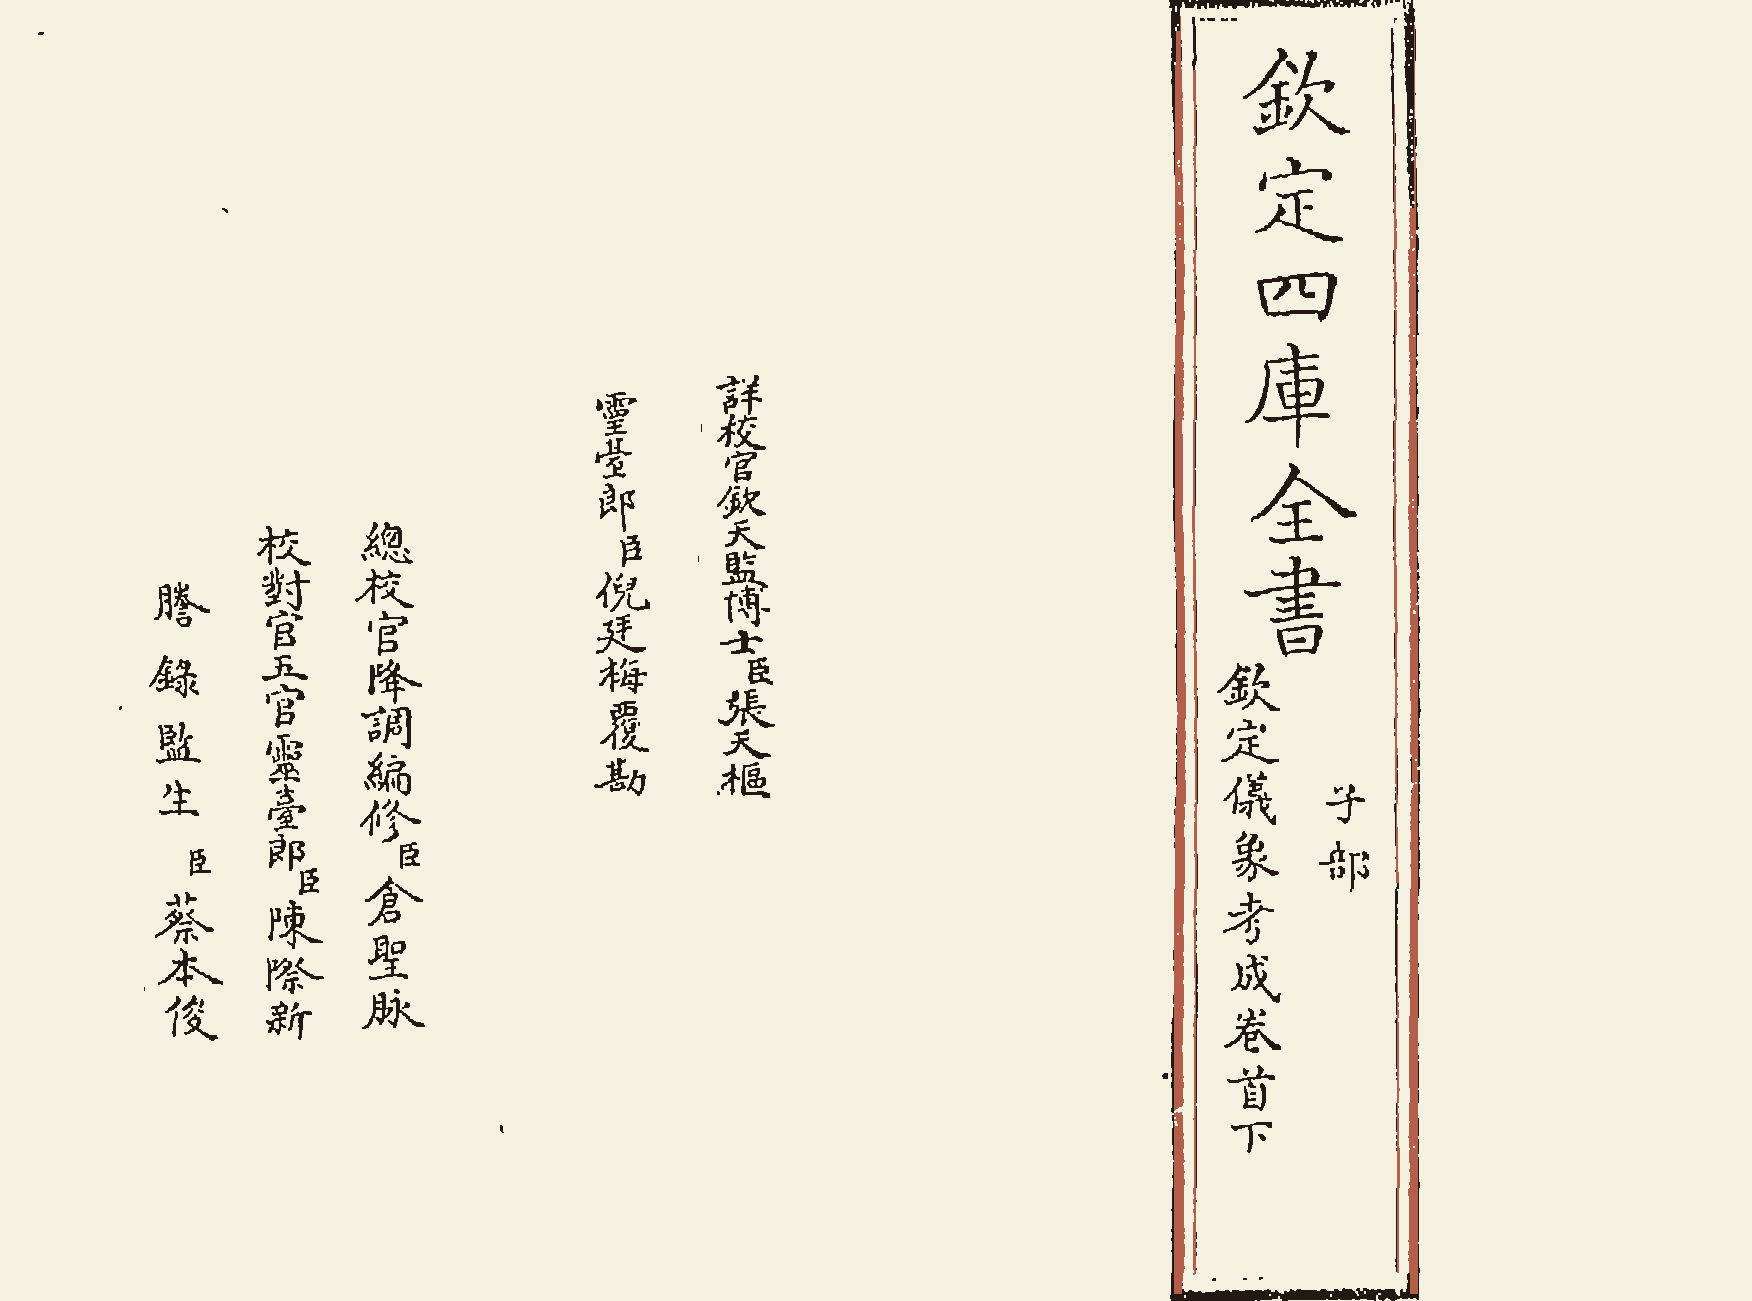
\includegraphics[width=\paperwidth,height=\paperheight,keepaspectratio]{img/0232.png}\clearpage
\begin{正文}
% ---- 册793 葉233 ----
\SetPageNumber{1}
欽定四庫全書\换行
欽定儀象考成卷首下\换行
御製璣衡撫辰儀説卷下\换行
　　用法\换行
　　算法\换行
\char"200B\relax\换行
\char"200B\relax\换行
\char"200B\relax\换行
\char"200B\relax\换行
\char"200B\relax\换行
\char"200B\relax\换行
\char"200B\relax\换行
\char"200B\relax\换行
\char"200B\relax\换行
\char"200B\relax\换行
\char"200B\relax
\par
% ---- 册793 葉236 ----
御製璣衡撫辰儀説卷下之一\换行
　用法\换行
　　測太陽時刻\换行
　　測日出入時刻及晝夜永短\换行
　　測太陽赤道緯度\换行
　　測午正太陽髙弧\换行
　　測太陽赤道經度\换行
　　測月星赤道經緯度\换行
　　測恒星求時刻\换行
　　測月五星求時刻\换行
　　測月星當中及偏度\换行
　　測月星出入地平時刻\换行
　　測南北真線\换行
　　測北極髙度\换行
　　測黄赤距度\换行
　　測黄白距度
\par
% ---- 册793 葉237 ----
　　測太陽時刻\换行
法以四遊圏東西推轉窺衡南北低昂令太陽從衡孔\换行
透光圓正或用薫黒玻璃置於下端衡孔視上端圓孔\换行
十字線正當太陽中心則窺衡與太陽參直乃視四遊\换行
圏下周指時度表臨於天常赤道之某時刻分即太陽\换行
時刻也若二分前後日影為赤道所礙則用窺衡上面\换行
立表測之\双列{\右小列{常時不為赤道所}\左小列{礙亦用此表為便}}若午正及卯酉前後日影\换行
為子午圏及龍柱所礙則用窺衡上面平行立表測之\换行
以四遊窺衡對凖太陽令上端表圓孔十字線影從下\换行
端表圓孔正中透出上端表直線影從下端表直縫正\换行
中透出\双列{\右小列{測時刻止用經度可止取直線影}\左小列{若測緯度則必取圓孔十字線影}}視指時度表\换行
所指即得太陽時刻若指時度表為子午圏所礙則易\换行
用借弧指時度表次用平行立表測定日影視借弧指\换行
時度表所指時刻加一小時即得太陽時刻盖借弧之\换行
長當遊旋赤道之十五度當天常赤道之一小時又借\换行
表在四遊圏之西所指時刻在本時前故加一小時即
\par
% ---- 册793 葉240 ----
為本時刻分也\换行
　　測日出入時刻及晝夜永短\换行
法於太陽出入地平時按前法測得太陽出入時刻乃\换行
計距午正前後若干刻分倍之即得晝刻計距子正前\换行
後若干刻分倍之即得夜刻\换行
　　測太陽赤道緯度\换行
法如前測凖太陽視窺衡下端指緯度表所指四遊圏\换行
右面距赤道度分即得太陽赤道緯度表指赤道北太\换行
陽緯度為在赤道南表指赤道南太陽緯度為在赤道\换行
北盖窺管以圓心為樞上端所窺在赤道北下端所指\换行
必在赤道南上端所窺在赤道南下端所指必在赤道\换行
北也\换行
　　測午正太陽髙弧\换行
法於午正時測得太陽赤道緯度在赤道北與赤道髙\换行
五十度五分相加在赤道南與赤道髙五十度五分相\换行
減即午正太陽髙弧也
\par
% ---- 册793 葉241 ----
　　測太陽赤道經度\换行
法用恒星作距測之取所知近午正前後一恒星\双列{\右小列{午正}\左小列{前後}}\换行
\双列{\右小列{取其𫎇氣少}\左小列{易得確凖也}}以其赤道經度之對衝用綰經度表於遊\换行
旋赤道綰定四遊圏\双列{\右小列{凡以儀器測星其上當星處為星}\左小列{之正位其下當人目處則星之對}}\换行
\双列{\右小列{冲故以星經度之對冲於}\左小列{遊旋赤道綰定四遊圏}}又任設一時用綰時度表於\换行
其時刻之對衝綰定天常赤道\双列{\右小列{天常環面乃日影所照}\左小列{之時其對冲則太陽所}}\换行
\双列{\右小列{臨之正位故於設時之對冲綰之如設丑正初}\左小列{刻則綰於未正初刻即太陽臨於丑正之位也}}乃将四\换行
逰圏帶定遊旋赤道用窺衡測凖距星隨之左旋𠉀至\换行
所設時刻\双列{\右小列{或鐘表或漏}\左小列{壺須得確凖}}視綰時度表對於遊旋赤道之\换行
某宫度分即太陽赤道經度也\双列{\右小列{環面時刻之對冲即太}\左小列{陽所臨之正位故其所}}\换行
\双列{\右小列{對遊旋赤道之宫}\左小列{度即太陽經度}}\换行
又法先以恒星作距測金星次以金星作距測太陽如\换行
金星晨見則於太陽未出之前取在金星西之一恒星\换行
作距以其赤道經度用平行線測經度表於遊旋赤道\换行
安定\双列{\右小列{三測皆係經度若距星之經度用對冲則測得之}\左小列{經度又須加減半周故距星不用對冲所測亦即}}\换行
\双列{\右小列{得本}\左小列{度也}}令一人用此平行線表窺定距星隨之左旋一人
\par
% ---- 册793 葉244 ----
用四遊窺衡測金星兩人同時測定乃視四遊圏指時\换行
度表所指遊旋赤道之宫度分即金星赤道經度次以\换行
金星赤道經度用平行線測經度表於遊旋赤道安定\换行
令一人窺定金星隨之左旋一人於太陽始出時用四\换行
遊窺衡測太陽乃視四遊圏指時度表所指遊旋赤道\换行
之宫度分即得太陽赤道經度若金星夕見則於太陽\换行
将入時任於某宫初度安定平行線測經度表令一人\换行
窺定金星又令一人用四遊窺衡測太陽視太陽距金\换行
星若干度記定俟太陽既入後取金星東之一恒星作\换行
距按前法測得金星赤道經度内減太陽距金星之度\换行
\双列{\右小列{星在東日}\左小列{在西故減}}即得太陽赤道經度也\双列{\右小列{太陽光大惟月及金}\左小列{星可以兩見然月有}}\换行
\双列{\右小列{視差不如用}\左小列{金星為凖也}}\换行
　　測月星赤道經緯度\换行
法於昏後曉前任設一時以本日太陽赤道經度與次\换行
日太陽赤道經度比例得本時太陽赤道經度\双列{\右小列{七政時}\左小列{憲書所}}\换行
\双列{\右小列{列乃子正之度子正後七政皆有行分故以本日子正}\左小列{之度分與次日子正之度分相減餘為一日十二時所}}
\par
% ---- 册793 葉245 ----
\双列{\右小列{行之分與設時距子正之時分為比例得設時距子}\左小列{正之行分加於本日子正之度分得本時之度分}}用\换行
綰時度表於遊旋赤道綰定又以所設時刻之對冲於\换行
天常赤道綰定𠉀至所設時刻用四遊窺衡測月星乃\换行
視指時度表所指遊旋赤道宫度加半周\双列{\右小列{環面時刻之}\左小列{對冲即為太}}\换行
\双列{\右小列{陽之正位環面之宮度却}\左小列{為月星之對冲故加半周}}即得所測月星赤道經度隨\换行
察指緯度表所指四遊圏距赤道南北度分即得所測\换行
月星赤道緯度也\双列{\右小列{緯之南北與前測}\左小列{太陽緯度法同}}\换行
又法用恒星作距測之以距星之赤道經度用平行線\换行
測經度表於遊旋赤道安定令一人用此平行線表窺\换行
定距星隨之左旋一人用四遊窺衡測月星兩人同時\换行
測定乃視指時度表所指遊旋赤道之度分即所測月\换行
星之赤道經度隨察指緯度表所指四遊圏之度分即\换行
得所測月星之赤道緯度也\换行
　　測恒星求時刻\换行
法先以恒星赤道經度用綰經度表於遊旋赤道綰定\换行
四遊圏次約計測時為某時依前法比例得本時太陽
\par
% ---- 册793 葉248 ----
赤道經度\双列{\右小列{太陽每日行一度於時為四分每一時行五}\左小列{分於時為二十秒故約計測量之時比例得}}\换行
\双列{\右小列{其時赤道經度即}\左小列{可用以測時刻也}}用綰時度表綰定遊旋赤道将四遊\换行
圏帶遊旋赤道推轉用窺衡測定恒星乃視綰時度表\换行
對於天常赤道之某時刻分加六時即太陽時刻也\双列{\右小列{天}\左小列{常}}\换行
\双列{\右小列{赤道之時刻乃日影對照之時故}\左小列{加六時始為太陽所臨之時刻也}}\换行
　　測月五星求時刻\换行
法以本時太陽赤道經度用綰時度表綰定遊旋赤道\换行
以月五星本時赤道經度之對冲用綰經度表於遊旋\换行
赤道綰定四遊圏将四遊圏帶遊旋赤道推轉用窺衡\换行
測定月星乃視綰時度表對於天常赤道之某時刻分\换行
加六時即得太陽時刻若太陽近子正前後綰時度表\换行
為子午圏所礙則向東或西借三十度綰定測之視所\换行
對時刻加減一時\双列{\右小列{向東借則加}\左小列{向西借則減}}即得太陽時刻若月五\换行
星近赤道或近午正前後為諸圏所礙則用窺管上面\换行
立表及平行立表測之與前測太陽時刻法同\换行
　　測月星當中及偏度
\par
% ---- 册793 葉249 ----
法以四遊窺衡隨時測月或星視指時度表當天常赤\换行
道之某時刻分記之\双列{\右小列{近午正則易用借弧}\左小列{指時度表加一小時}}午正為當中\换行
無偏度午正前為偏東午正後為偏西乃以距午時分\换行
變赤道度每一時為三十度每一小時為十五度每一\换行
分為十五分每一秒為十五秒共之為所偏度凡推月\换行
星當中及偏度者用此法測之則離合可辨凡有求時\换行
刻者用此法測定則時刻可推也\换行
　　測月星出入地平時刻\换行
法以本日子正月五星赤道經度或恒星經度之對冲\换行
用綰經度表於遊旋赤道綰定四遊圏又以本日子正\换行
太陽經度用綰時度表綰定遊旋赤道爰以四遊窺衡\换行
於月星出入地平時測之視綰時度表當天常赤道之\换行
某時刻分加六時為本日月星出入時刻之通數復計\换行
測時距本日子正後若干時刻比例得太陽行分變時\换行
\双列{\右小列{每一度為四分每十五分}\左小列{為一分每十五秒為一秒}}為太陽時差比例得月五星\换行
行分變時為月五星時差\双列{\右小列{恒星則無行}\左小列{分亦無時差}}乃於前所測月
\par
% ---- 册793 葉252 ----
星出入時刻之通數減太陽時差加月五星時差即得\换行
月星出入地平時刻盖日與月星測時皆用子正經度\换行
而子正後太陽有右旋之行分則時刻必差而早月五\换行
星亦有右旋之行分則時刻必差而遲\双列{\右小列{時刻左旋七政}\左小列{皆右旋太陽有}}\换行
\双列{\右小列{右旋之行分則測時太陽之經度必在所測時刻之前}\左小列{故差而早月五星有右旋之行分則測時月星之方位}}\换行
\双列{\右小列{必在所測時刻}\左小列{之後故差而遲}}故減太陽時差加月五星時差\双列{\右小列{若五星}\左小列{逆行則}}\换行
\双列{\右小列{時差}\左小列{亦減}}方為月星出入地平真時此與前測月星求時刻\换行
法同理設時可以預知故先求本時經度而後測月星\换行
出入難以懸定故先測而後加減時差其理相通其用\换行
尤便也\换行
　　測南北真線\换行
法於太陽出地平時測其距午東赤道度又於太陽入\换行
地平時測其距午西赤道度\双列{\右小列{測得太陽出入地平距午}\左小列{正前後若干時分變赤道}}\换行
\双列{\右小列{度即得距午正}\左小列{東西赤道度}}兩距午度相等則子午圏之向即南北\换行
真線若日出距午東之度多日入距午西之度少則子\换行
午圏之午正偏西若日出距午東之度少日入距午西
\par
% ---- 册793 葉253 ----
之度多則子午圏之午正偏東\双列{\右小列{此言午正乃子}\左小列{午圏之正南}}以兩測\换行
之距午度相減折半即所偏之赤道經度\双列{\右小列{若求地平偏}\左小列{度則用三角}}\换行
\双列{\右小列{法推之見算}\左小列{法第八則}}依所偏之度作線即南北真線也\换行
又法於冬至後測織女第一星昏刻此星當酉正之位\换行
以四遊圏安於酉正測其去極度若干\双列{\右小列{九十度内減赤}\左小列{道緯度餘即去}}\换行
\双列{\右小列{極}\左小列{度}}旦刻此星當卯正之位以四遊圏安於卯正測其去\换行
極度若干\双列{\右小列{織女星在赤道丑宫七度赤道北三十八度}\左小列{半冬至後半月内昏旦可以兩見故専取此}}\换行
\双列{\右小列{星測}\左小列{之}}兩去極度相等則子午圏之向即南北真線若卯\换行
正位測得去極度多酉正位測得去極度少則東逺西\换行
近即子午圈之北極偏西若卯正位測得去極度少酉\换行
正位測得去極度多則東近西逺即子午圈之北極偏\换行
東以兩測之去極度相減折半即所偏之赤道緯度\双列{\右小列{若}\左小列{求}}\换行
\双列{\右小列{地平偏度則用三角法}\左小列{推之見算法第十五則}}依所偏之度作線即南北真線\换行
也盖南北真線自北極過天頂平分赤道之地平上半\换行
周是為午正故向南測者以午正為凖向北測者以北\换行
極為凖太陽隨天左旋其出地入地距午必相等若其
\par
% ---- 册793 葉256 ----
不等必儀之午正偏也恒星繞地左旋其在東在西去\换行
極必相等若其不等必儀之北極偏也依其偏度正之\换行
則南北真線得矣又按渾儀經緯與天同象測太陽亦\换行
可用緯度測恒星亦可用經度然不及右二法之簡明\换行
推測精熟法理自見今不具悉也\换行
　　測北極髙度\换行
法於冬至前後以四遊圏安於正北測天權星\双列{\右小列{即北斗}\左小列{第四星}}\换行
昏刻此星在北極之下測其去極度若干旦刻此星在\换行
北極之上測其去極度若干\双列{\右小列{天權星今在赤道辰宫初}\左小列{度赤道北五十八度冬至}}\换行
\双列{\右小列{前後半月内昏旦可以}\左小列{兩見故専取此星測之}}兩去極度相等則儀之北極髙\换行
度與天合若在上之去極度少在下之去極度多則儀\换行
之北極差髙若在上之去極度多在下之去極度少則\换行
儀之北極差下以兩測之去極度相減折半即所差之\换行
地平緯度於儀之北極髙度加減之\双列{\右小列{差髙則減}\左小列{差下則加}}即天之\换行
北極髙度也盖天之北極無星故取大星之環繞北極\换行
上下者測之星之去極有定度則上下兩測之去極必
\par
% ---- 册793 葉257 ----
等若其不等則儀之髙下差也依其差度加減之則在\换行
天之北極髙度得矣又按舊法用地平緯儀測鉤陳大\换行
星以其在北極上下兩髙度相加折半得北極髙度取\换行
其距地髙無𫎇氣也今用渾儀測之則鉤陳大星為儀\换行
樞所礙須用借弧故取用天權星測其去極之較以備\换行
一例若以所測在北極上之去極度與所設北極髙度\换行
相加以所測在北極下之去極度與所設北極髙度相\换行
減得兩地平髙度相加折半得北極髙度與用鉤陳大\换行
星之理同\换行
　　測黄赤大距\换行
法於冬至日午正初刻測太陽在赤道南若干度分夏\换行
至日午正初刻測太陽在赤道北若干度分若冬至夏\换行
至皆在午正初刻則所測日距赤道南北之緯度即黄\换行
赤大距度若冬至夏至不正當午正則又用前測太陽\换行
赤道經度法測得太陽距冬夏至前後若干度分用有\换行
太陽赤道經緯度求黄赤交角之法\双列{\右小列{見算法}\左小列{第四則}}求得黄赤
\par
% ---- 册793 葉260 ----
交角即黄赤大距度也盖黄道與赤道斜交春秋分時\换行
太陽正當赤道春分後秋分前太陽在赤道北夏至而\换行
極北秋分後春分前太陽在赤道南冬至而極南故致\换行
日者必於冬夏二至今用弧線三角形法測得逐日之\换行
距緯皆可以推大距然春秋分前後黄道斜而緯差大\换行
以推大距其理𨼆而難知冬夏至前後黄道横而緯差\换行
微以推大距其象顯而易見故冬夏致日古今之通義\换行
也\换行
　　測黄白距限\双列{\右小列{距限即大距因大距又有大小故}\左小列{名距限以别之見數象考成後編}}\换行
法於春分日上弦秋分日下弦月距交九十度時測得\换行
月距赤道北若干度分春分日下弦秋分日上弦月距\换行
交九十度時測得月距赤道南若干度分與黄赤大距\换行
相減餘為黄白二道最大之距限又於冬至日望月距\换行
交九十度時測得月距赤道北若干度分夏至日望月\换行
距交九十度時測得月距赤道南若干度分與黄赤大\换行
距相減餘為黄白二道最小之距限盖白道與黄道斜
\par
% ---- 册793 葉261 ----
交月距交九十度則距黄道最逺故測黄白大距必於\换行
月距交九十度時然黄白大距與黄道成直角黄赤大\换行
距與赤道成直角惟冬夏二至黄道經圈與赤道經圈\换行
合為一線故測黄白大距又必於月當冬夏二至時\双列{\右小列{上}\左小列{編}}\换行
\双列{\右小列{専取月當夏至為其距地髙也}\左小列{若以對待而言則兼用冬夏至}}夫月距交九十度而又\换行
當冬夏二至則兩交必在春秋二分當是時而值兩弦\换行
則日必在春秋分而適當兩交值朔望則日必在冬夏\换行
至而距交九十度上編之法謂兩弦時交角大\双列{\右小列{交角之}\左小列{度即大}}\换行
\双列{\右小列{距}\左小列{度}}朔望時交角小後編之法謂日在兩交時交角大日\换行
距交九十度時交角小極二説之異致至此而得其合\换行
故測黄白大距必於春秋分兩弦冬夏至望日\双列{\右小列{朔日不}\左小列{見月故}}\换行
\双列{\右小列{惟用}\左小列{望日}}月距交九十度時測之春分之日上弦秋分之日\换行
下弦而月距交九十度是月當夏至而日在兩交也春\换行
分之日下弦秋分之日上弦而月距交九十度是月當\换行
冬至而日在兩交也以兩弦與日在兩交而論皆交角\换行
大冬至之日望而月距交九十度是月當夏至而日距
\par
% ---- 册793 葉264 ----
交九十度也夏至之日望而月距交九十度是月當冬\换行
至而日距交九十度也以朔望與日距交九十度而論\换行
皆交角小各測其距赤道度與黄赤大距相減則最大\换行
最小之黄白距限皆得矣按月行出黄道南為陽厯為\换行
正交\双列{\右小列{今為}\左小列{中交}}入黄道北為陰厯為中交\双列{\右小列{今為}\左小列{正交}}夏至在陰厯\换行
冬至在陽厯則月距赤道校黄道為逺故於所測距赤\换行
道度内減黄赤大距餘為黄白大距夏至在陽厯冬至\换行
在陰厯則月距赤道校黄道為近故於黄赤大距内減\换行
所測距赤道度餘為黄白大距又按古法黄白大距不\换行
逾六度弦望無殊故曰春秋致月今法交角有大小故\换行
又必兼於冬夏至測之也\换行
又法推得月離黄道冬夏至時預於前數刻或以太陽\换行
作距用綰時度表綰定時刻或以恒星作距用平行線\换行
測經度表對定距星皆以四遊圏指時度表對冬夏至\换行
宫度安定候月行至二至線上乃以窺衡測月距赤道\换行
南北緯度若干與黄赤大距相減餘為月距黄道南北
\par
% ---- 册793 葉265 ----
緯度以正交宫度與冬夏至宫度相減餘為月距正交\换行
黄道經度用有太陽赤道經緯度求黄赤交角之法\双列{\右小列{見}\左小列{算}}\换行
\双列{\右小列{法第}\左小列{四則}}求得交角度分即黄白距限盖月之緯度與黄道\换行
成直角其三角形之比例則黄道如赤道白道如黄道\换行
黄緯如赤緯黄白交角即如黄赤交角黄白大距即如\换行
黄赤大距也前法於分至弦望測月緯度乃測黄白大\换行
距正法然其時不易得此法於月離冬夏至時凡見月\换行
即可測叅之弦望與日距交之逺近則交角有大小之\换行
故亦可得而稽矣\换行
\char"200B\relax\换行
\char"200B\relax\换行
\char"200B\relax\换行
\char"200B\relax\换行
\char"200B\relax\换行
\char"200B\relax\换行
\char"200B\relax
\par
% ---- 册793 葉268 ----
御製璣衡撫辰儀説下之二\换行
　算法\换行
　　有太陽赤道緯度求午正髙弧\换行
　　有太陽視髙弧求午正晷影\换行
　　有太陽赤道緯度求赤道經度\换行
　　有太陽赤道經緯度求黄赤大距\换行
　　有太陽赤道緯度求黄道經度\换行
　　有太陽赤道緯度求出入地平及晝夜時刻\换行
　　有太陽赤道緯度求昏旦時刻\换行
　　有太陽赤道緯度求太陽出入地平偏度\双列{\右小列{二題}\左小列{}}\换行
　　有時刻有太陽赤道緯度求地平經緯度\换行
　　有節氣有太陽午正髙弧求交節氣時刻\换行
　　有日月星赤道經度求月星當中時刻\换行
　　有日月星赤道經度有時刻求月星當中及偏度\换行
　　有日月星赤道經緯度求月星出入地平時刻\换行
　　有月星赤道經緯度求黄道經緯度
\par
% ---- 册793 葉269 ----
　　有月星距午赤道度有赤道緯度求地平經緯度\换行
　　有二星赤道經緯度求二星斜距度\换行
　　有日月五星視髙度求實髙度\换行
\char"200B\relax\换行
\char"200B\relax\换行
\char"200B\relax\换行
\char"200B\relax\换行
\char"200B\relax\换行
\char"200B\relax\换行
\char"200B\relax\换行
\char"200B\relax\换行
\char"200B\relax\换行
\char"200B\relax\换行
\char"200B\relax\换行
\char"200B\relax\换行
\char"200B\relax
\par
\end{正文}\clearpage
\contentSetup{n-char-per-col = 20, n-column = 9}
\begin{正文}
\end{正文}
\嵌图{259.22pt}{211.13pt}{687.10pt}{283.77pt}{img/0272.png}
\begin{正文}
% ---- 册793 葉272 ----
\SetPageNumber{20}
設如北極出地三十九度五十五分午正初刻測得\换行
　太陽距赤道北十五度求髙弧幾何\换行
　　　　　　　　　　如圖甲為天頂甲乙丙丁\换行
　　　　　　　　　　為子午圏乙丙為地平丁\换行
　　　　　　　　　　為北極戊己為赤道丁丙\换行
　　　　　　　　　　為北極出地三十九度五\换行
　　　　　　　　　　十五分戊乙為赤道髙五\换行
　　　　　　　　　　十度五分庚為太陽庚戊\换行
　　　　　　　　　　為太陽距赤道北十五度\换行
　　　　　　　　　　庚乙為太陽髙弧太陽正\换行
　　　　　　　　　　當午正赤經與髙弧合則\换行
　　　　　　　　　　以庚戊距緯與戊乙赤道\换行
　　　　　　　　　　髙度相加得庚乙六十五\换行
　　　　　　　　　　度五分為午正太陽髙度\换行
　　　　　　　　　　若太陽距赤道南則以距\换行
　　　　　　　　　　緯與赤道髙度相減即午\换行
　　　　　　　　　　正太陽髙度也\换行
設如測得午正太陽髙弧四十度中表髙八尺求影
\par
\end{正文}\clearpage
\嵌图{211.28pt}{218.24pt}{643.91pt}{276.65pt}{img/0273.png}
\begin{正文}
% ---- 册793 葉273 ----
\SetPageNumber{21}
　長幾何\换行
　　　　　　　　　　法以半徑一千萬為一率\换行
　　　　　　　　　　午正太陽髙弧四十度之\换行
　　　　　　　　　　餘切一千一百九十一萬\换行
　　　　　　　　　　七千五百三十六為二率\换行
　　　　　　　　　　表髙八尺為三率求得四\换行
　　　　　　　　　　率九尺五寸三分四釐零\换行
　　　　　　　　　　二絲八忽八微為所求之\换行
　　　　　　　　　　影長也如圖甲乙為中表\换行
　　　　　　　　　　之髙丙為太陽丁為中影\换行
　　　　　　　　　　心甲丁乙角為午正太陽\换行
　　　　　　　　　　髙度乙丁為影長則以丁\换行
　　　　　　　　　　戊半徑與太陽髙弧餘切\换行
　　　　　　　　　　戊已之比同於甲乙表髙\换行
　　　　　　　　　　與乙丁影長之比也\换行
設如春分後測得太陽距赤道北十五度黄赤交角\换行
　二十三度二十九分求赤道經度幾何\换行
　　　　　　　　　　如圖甲乙丙丁為赤道甲
\par
\end{正文}\clearpage
\嵌图{171.14pt}{215.35pt}{820.73pt}{279.54pt}{img/0276.png}
\begin{正文}
% ---- 册793 葉276 ----
\SetPageNumber{22}
\插图页
　　　　　　　　　　戊丙己為黄道相交於甲\换行
　　　　　　　　　　丙甲為春分丙為秋分戊\换行
　　　　　　　　　　為夏至己為冬至庚為北\换行
　　　　　　　　　　極辛為南極庚戊乙辛己\换行
　　　　　　　　　　丁為過二極二至經圈乙\换行
　　　　　　　　　　至戊丁至己俱二十三度\换行
　　　　　　　　　　二十九分為黄赤大距即\换行
　　　　　　　　　　甲丙黄赤二道相交之角\换行
　　　　　　　　　　壬為太陽甲壬為太陽距\换行
\恢复丝栏
　　　　　　　　　　春分後黄道經度自庚辛\换行
　　　　　　　　　　南北二極過太陽壬作庚\换行
　　　　　　　　　　壬癸辛赤極經圏交赤道\换行
　　　　　　　　　　於癸癸點為太陽所當赤\换行
　　　　　　　　　　道宫度甲癸為太陽距春\换行
　　　　　　　　　　分後赤道經度壬癸為太\换行
　　　　　　　　　　陽距赤道北十五度法用\换行
　　　　　　　　　　甲壬癸正弧三角形有甲\换行
　　　　　　　　　　角黄赤交角有癸直角有
\par
\end{正文}\clearpage
\嵌图{176.39pt}{207.01pt}{769.93pt}{287.88pt}{img/0277.png}
\begin{正文}
% ---- 册793 葉277 ----
\SetPageNumber{23}
\插图页
　　　　　　　　　　壬癸距緯求甲癸赤道度\换行
　　　　　　　　　　以甲角二十三度二十九\换行
　　　　　　　　　　分之乙子正切四百三十\换行
　　　　　　　　　　四萬四千六百六十六為\换行
　　　　　　　　　　一率乙丑半徑一千萬為\换行
　　　　　　　　　　二率壬癸距緯十五度之\换行
　　　　　　　　　　癸寅正切二百六十七萬\换行
　　　　　　　　　　九千四百九十二為三率\换行
　　　　　　　　　　求得四率六百一十六萬\换行
\恢复丝栏
　　　　　　　　　　七千三百一十四為甲癸\换行
　　　　　　　　　　弧之正弦癸卯檢表得三\换行
　　　　　　　　　　十八度四分四十秒即甲\换行
　　　　　　　　　　癸太陽距春分後赤道經\换行
　　　　　　　　　　度與甲丁春分距冬至三\换行
　　　　　　　　　　宫相加得四宫八度四分\换行
　　　　　　　　　　四十秒即太陽赤道宫度\换行
　　　　　　　　　　也\换行
設如春分後測得太陽距赤道北十五度距春分後
\par
\end{正文}\clearpage
\嵌图{268.26pt}{209.25pt}{723.62pt}{285.65pt}{img/0280.png}
\begin{正文}
% ---- 册793 葉280 ----
\SetPageNumber{24}
　赤道經度三十八度四分四十秒求黄赤大距度\换行
　幾何\换行
　　　　　　　　　　如圖甲為春分甲角為黄\换行
　　　　　　　　　　赤交角當戊乙黄赤大距\换行
　　　　　　　　　　壬為太陽壬癸為太陽距\换行
　　　　　　　　　　赤道北十五度甲癸為太\换行
　　　　　　　　　　陽距春分後赤道經度三\换行
　　　　　　　　　　十八度四分四十秒用甲\换行
　　　　　　　　　　壬癸正弧三角形以甲癸\换行
　　　　　　　　　　赤道三十八度四分四十\换行
　　　　　　　　　　秒之癸卯正弦六百一十\换行
　　　　　　　　　　六萬七千三百一十四為\换行
　　　　　　　　　　一率壬癸距緯十五度之\换行
　　　　　　　　　　寅癸正切二百六十七萬\换行
　　　　　　　　　　九千四百九十二為二率\换行
　　　　　　　　　　乙丑半徑一千萬為三率\换行
　　　　　　　　　　求得四率四百三十四萬\换行
　　　　　　　　　　六千六百六十六為甲角
\par
\end{正文}\clearpage
\嵌图{598.94pt}{210.20pt}{392.93pt}{284.70pt}{img/0281.png}
\嵌图{144.29pt}{217.63pt}{132.27pt}{277.27pt}{img/0281_1.png}
\begin{正文}
% ---- 册793 葉281 ----
\SetPageNumber{25}
　　　　　　　　　　之正切乙子檢表得二十\换行
　　　　　　　　　　三度二十九分即甲角黄\换行
　　　　　　　　　　赤大距度也\换行
設如春分後測得太陽距赤道北十五度黄赤交角\换行
　二十三度二十九分求黄道經度幾何\换行
　　　　　　　　　　如圖甲為春分甲角為黄\换行
　　　　　　　　　　赤交角二十三度二十九\换行
　　　　　　　　　　分壬為太陽甲壬為太陽\换行
　　　　　　　　　　距春分後黄道經度壬癸\换行
　　　　　　　　　　為距赤道北十五度用甲\换行
　　　　　　　　　　壬癸正弧三角形有甲角\换行
　　　　　　　　　　黄赤交角有癸直角有壬\换行
　　　　　　　　　　癸距緯求甲壬黄道度以\换行
　　　　　　　　　　甲角二十三度二十九分\换行
　　　　　　　　　　之戊辰正弦三百九十八\换行
　　　　　　　　　　萬四千八百二十三為一\换行
　　　　　　　　　　率戊丑半徑一千萬為二\换行
　　　　　　　　　　率壬癸距緯十五度之壬
\par
\end{正文}\clearpage
\嵌图{723.65pt}{204.84pt}{268.22pt}{290.06pt}{img/0284.png}
\嵌图{167.32pt}{219.20pt}{382.61pt}{275.69pt}{img/0284_1.png}
\begin{正文}
% ---- 册793 葉284 ----
\SetPageNumber{26}
　　　　　　　　　　巳正弦二百五十八萬八\换行
　　　　　　　　　　千一百九十為三率求得\换行
　　　　　　　　　　四率六百四十九萬五千\换行
　　　　　　　　　　一百一十九為甲壬弧之\换行
　　　　　　　　　　正弦壬午檢表得四十度\换行
　　　　　　　　　　三十分十七秒即甲壬太\换行
　　　　　　　　　　陽距春分後黄道經度與\换行
　　　　　　　　　　甲已春分距冬至三宫相\换行
　　　　　　　　　　加得四宫十度三十分十\换行
　　　　　　　　　　七秒即太陽黄道宫度也\换行
設如北極出地三十九度五十五分測得太陽距赤\换行
　道北十五度求出入地平及晝夜時刻\换行
　　　　　　　　　　如圖甲為天頂甲乙丙丁\换行
　　　　　　　　　　為子午圏乙丙為地平丁\换行
　　　　　　　　　　為北極丁丙為北極出地\换行
　　　　　　　　　　三十九度五十五分戊己\换行
　　　　　　　　　　為赤道戊乙為赤道髙五\换行
　　　　　　　　　　十度零五分庚為太陽庚
\par
\end{正文}\clearpage
\嵌图{163.37pt}{218.18pt}{386.56pt}{276.72pt}{img/0285.png}
\begin{正文}
% ---- 册793 葉285 ----
\SetPageNumber{27}
　　　　　　　　　　辛為太陽距赤道北十五\换行
　　　　　　　　　　度壬為卯正酉正之位辛\换行
　　　　　　　　　　壬為日出入在卯前酉後\换行
　　　　　　　　　　赤道度用庚辛壬正弧三\换行
　　　　　　　　　　角形有辛直角有壬角赤\换行
　　　　　　　　　　道髙度有庚辛邊求辛壬\换行
　　　　　　　　　　邊以壬角五十度五分之\换行
　　　　　　　　　　正切一千一百九十五萬\换行
　　　　　　　　　　二千七百九十九為一率\换行
　　　　　　　　　　半徑一千萬為二率庚辛\换行
　　　　　　　　　　十五度之正切二百六十\换行
　　　　　　　　　　七萬九千四百九十二為\换行
　　　　　　　　　　三率求得四率二百二十\换行
　　　　　　　　　　四萬一千七百二十八為\换行
　　　　　　　　　　辛壬弧之正弦檢表得十\换行
　　　　　　　　　　二度五十七分十五秒即\换行
　　　　　　　　　　辛壬弧為日出入在卯前\换行
　　　　　　　　　　酉後赤道度變時得三刻
\par
\end{正文}\clearpage
\嵌图{171.14pt}{215.05pt}{820.73pt}{279.84pt}{img/0288.png}
\begin{正文}
% ---- 册793 葉288 ----
\SetPageNumber{28}
\插图页
　　　　　　　　　　六分四十九秒為卯前酉\换行
　　　　　　　　　　後分以減卯正得日出卯\换行
　　　　　　　　　　初初刻八分十一秒以加\换行
　　　　　　　　　　酉正得日入酉正三刻六\换行
　　　　　　　　　　分四十九秒復倍卯前酉\换行
　　　　　　　　　　後分得六刻十三分三十\换行
　　　　　　　　　　八秒與四十八刻相加得\换行
　　　　　　　　　　五十四刻十三分三十八\换行
　　　　　　　　　　秒為晝刻與四十八刻相\换行
\恢复丝栏
　　　　　　　　　　減得四十一刻一分二十\换行
　　　　　　　　　　二秒為夜刻也又法求己\换行
　　　　　　　　　　辛日出入距子正前後赤\换行
　　　　　　　　　　道度用丁丙庚正弧三角\换行
　　　　　　　　　　形有丙直角有丁丙北極\换行
　　　　　　　　　　出地度有丁庚日距北極\换行
　　　　　　　　　　度求丁角以丁庚七十五\换行
　　　　　　　　　　度之正切三千七百三十\换行
　　　　　　　　　　二萬零五百零八為一率
\par
\end{正文}\clearpage
\嵌图{612.78pt}{223.00pt}{379.10pt}{271.90pt}{img/0289.png}
\嵌图{163.01pt}{219.31pt}{386.92pt}{275.58pt}{img/0289_1.png}
\begin{正文}
% ---- 册793 葉289 ----
\SetPageNumber{29}
　　　　　　　　　　丁丙三十九度五十五分\换行
　　　　　　　　　　之正切八百三十六萬六\换行
　　　　　　　　　　千二百四十二為二率半\换行
　　　　　　　　　　徑一千萬為三率求得四\换行
　　　　　　　　　　率二百二十四萬一千七\换行
　　　　　　　　　　百二十八為丁角之餘弦\换行
　　　　　　　　　　檢表得七十七度二分四\换行
　　　　　　　　　　十五秒即辛已弧為日出\换行
　　　　　　　　　　入距子正前後赤道度變\换行
　　　　　　　　　　時得五小時零八分十一\换行
　　　　　　　　　　秒為日出入距子正前後\换行
　　　　　　　　　　分自子正起算為卯初初\换行
　　　　　　　　　　刻八分十一秒即日出時\换行
　　　　　　　　　　刻與二十四小時相減得\换行
　　　　　　　　　　酉正三刻六分四十九秒\换行
　　　　　　　　　　為日入時刻復倍日出入\换行
　　　　　　　　　　距子正前後分得四十一\换行
　　　　　　　　　　刻一分二十二秒為夜刻
\par
\end{正文}\clearpage
\嵌图{605.32pt}{212.83pt}{386.56pt}{282.06pt}{img/0292.png}
\begin{正文}
% ---- 册793 葉292 ----
\SetPageNumber{30}
　　　　　　　　　　與九十六刻相減餘五十\换行
　　　　　　　　　　四刻十三分三十八秒為\换行
　　　　　　　　　　晝刻也\换行
設如北極出地三十九度五十五分測得太陽距赤\换行
　道北十五度求昏旦時刻\换行
　　　　　　　　　　如圖甲為天頂甲乙丙丁\换行
　　　　　　　　　　為子午圈乙丙為地平丁\换行
　　　　　　　　　　為北極丁丙為北極出地\换行
　　　　　　　　　　三十九度五十五分甲丁\换行
\插图页
　　　　　　　　　　為北極距天頂五十度五\换行
　　　　　　　　　　分戊己為赤道庚為太陽\换行
　　　　　　　　　　庚辛為太陽距赤道北十\换行
　　　　　　　　　　五度丁庚為太陽距北極\换行
　　　　　　　　　　七十五度壬癸為太陽隨\换行
　　　　　　　　　　天西轉之赤道距等圈庚\换行
　　　　　　　　　　子為昏旦曚影限十八度\换行
　　　　　　　　　　甲庚為太陽距天頂一百\换行
　　　　　　　　　　零八度丑寅為地平下曚
\恢复丝栏
\par
\end{正文}\clearpage
\嵌图{171.43pt}{217.40pt}{820.44pt}{277.49pt}{img/0293.png}
\begin{正文}
% ---- 册793 葉293 ----
\SetPageNumber{31}
\插图页
　　　　　　　　　　影距等圈辛點為太陽所\换行
　　　　　　　　　　當昏旦時刻戊辛為太陽\换行
　　　　　　　　　　距午正前後赤道度用甲\换行
　　　　　　　　　　庚丁斜弧三角形有甲丁\换行
　　　　　　　　　　邊北極距天頂有丁庚邊\换行
　　　　　　　　　　日距北極有甲庚邊日距\换行
　　　　　　　　　　天頂求丁角距午赤道度\换行
　　　　　　　　　　以夾丁角之丁庚邊七十\换行
　　　　　　　　　　五度與甲丁邊五十度五\换行
\恢复丝栏
　　　　　　　　　　分相加得一百二十五度\换行
　　　　　　　　　　五分為總弧其餘弦五百\换行
　　　　　　　　　　七十四萬七千六百七十\换行
　　　　　　　　　　二又以甲丁丁庚二邊相\换行
　　　　　　　　　　減餘二十四度五十五分\换行
　　　　　　　　　　為較弧其餘弦九百零六\换行
　　　　　　　　　　萬九千二百一十五兩餘\换行
　　　　　　　　　　弦相加\双列{\右小列{總弧較弧一過象}\左小列{限一不過象限則}}\换行
　　　　　　　　　　\双列{\右小列{兩餘弦相加若兩弧俱不}\左小列{過象限或俱過象限則兩}}
\par
\end{正文}\clearpage
\嵌图{192.65pt}{215.83pt}{799.22pt}{279.06pt}{img/0296.png}
\begin{正文}
% ---- 册793 葉296 ----
\SetPageNumber{32}
\插图页
　　　　　　　　　　\双列{\右小列{餘弦}\左小列{相減}}得一千四百八十一\换行
　　　　　　　　　　萬六千八百八十七折半\换行
　　　　　　　　　　得七百四十萬零八千四\换行
　　　　　　　　　　百四十四為中數為一率\换行
　　　　　　　　　　以對丁角之甲庚邊一百\换行
　　　　　　　　　　零八度之大矢一千三百\换行
　　　　　　　　　　零九萬零一百七十\双列{\右小列{餘弦}\左小列{與半}}\换行
　　　　　　　　　　\双列{\右小列{徑相加}\左小列{得大矢}}與較弧二十四度\换行
　　　　　　　　　　五十五分之正矢\双列{\右小列{餘弦與}\左小列{半徑相}}\换行
\恢复丝栏
　　　　　　　　　　\双列{\右小列{減得}\左小列{正矢}}九百三十萬零七百\换行
　　　　　　　　　　八十五相減餘一千二百\换行
　　　　　　　　　　一十五萬九千三百八十\换行
　　　　　　　　　　五為矢較為二率半徑一\换行
　　　　　　　　　　千萬為三率求得四率一\换行
　　　　　　　　　　千六百四十一萬二千八\换行
　　　　　　　　　　百七十三為丁角之大矢\换行
　　　　　　　　　　\双列{\右小列{凡矢過於半徑者為}\左小列{大矢其角即為鈍角}}内減\换行
　　　　　　　　　　半徑一千萬餘六百四十
\par
\end{正文}\clearpage
\嵌图{182.48pt}{211.52pt}{809.40pt}{283.38pt}{img/0297.png}
\begin{正文}
% ---- 册793 葉297 ----
\SetPageNumber{33}
\插图页
　　　　　　　　　　一萬二千八百七十三為\换行
　　　　　　　　　　丁角之餘弦檢表得五十\换行
　　　　　　　　　　度六分四十四秒與半周\换行
　　　　　　　　　　相減餘一百二十九度五\换行
　　　　　　　　　　十三分十六秒為丁角度\换行
　　　　　　　　　　即旦刻太陽距午前昏刻\换行
　　　　　　　　　　太陽距午後赤道度變時\换行
　　　　　　　　　　得八小時二刻九分三十\换行
　　　　　　　　　　三秒與午正十二小時相\换行
\恢复丝栏
　　　　　　　　　　減得寅初一刻五分二十\换行
　　　　　　　　　　七秒即旦刻與午正十二\换行
　　　　　　　　　　小時相加得戌正二刻九\换行
　　　　　　　　　　分三十三秒即昏刻也如\换行
　　　　　　　　　　圖丁庚與丁甲相加得甲\换行
　　　　　　　　　　癸為總弧\双列{\右小列{丁庚丁癸丁壬}\左小列{三弧同為癸壬}}\换行
　　　　　　　　　　\双列{\右小列{距等圏所截}\左小列{故其度相等}}其正弦為癸\换行
　　　　　　　　　　卯餘弦為卯辰丁庚與丁\换行
　　　　　　　　　　甲相減餘甲壬為較弧其
\par
\end{正文}\clearpage
\嵌图{167.23pt}{203.63pt}{824.64pt}{291.26pt}{img/0300.png}
\begin{正文}
% ---- 册793 葉300 ----
\SetPageNumber{34}
\插图页
　　　　　　　　　　正弦為壬己餘弦為己辰\换行
　　　　　　　　　　以卯辰與己辰兩餘弦相\换行
　　　　　　　　　　加得巳卯折半得己午與\换行
　　　　　　　　　　未申等為中數又對丁角\换行
　　　　　　　　　　之甲庚邊與甲丑甲寅等\换行
　　　　　　　　　　其正弦為丑酉或寅酉餘\换行
　　　　　　　　　　弦為酉辰大矢為甲酉以\换行
　　　　　　　　　　甲酉與甲壬較弧之正矢\换行
　　　　　　　　　　甲已相減餘己酉與戌庚\换行
\恢复丝栏
　　　　　　　　　　等為矢較遂成壬庚戌與\换行
　　　　　　　　　　壬申未同式兩勾股形故\换行
　　　　　　　　　　未申與戌庚之比必同於\换行
　　　　　　　　　　壬申與壬庚之比也又戊\换行
　　　　　　　　　　辰為半徑壬申為距等圈\换行
　　　　　　　　　　之半徑壬庚與戊辛兩叚\换行
　　　　　　　　　　同為丁庚辛赤道經圏之\换行
　　　　　　　　　　所分則壬申與壬庚之比\换行
　　　　　　　　　　原同於戊辰與戊辛之比
\par
\end{正文}\clearpage
\嵌图{155.20pt}{208.44pt}{394.73pt}{286.46pt}{img/0301.png}
\begin{正文}
% ---- 册793 葉301 ----
\SetPageNumber{35}
\插图页
　　　　　　　　　　是以中數未申與矢較戌\换行
　　　　　　　　　　庚之比即同於半徑戊辰\换行
　　　　　　　　　　與丁角大矢戊辛之比也\换行
　　　　　　　　　　既得戊辛大矢内減戊辰\换行
　　　　　　　　　　半徑餘辛辰即丁外角餘\换行
　　　　　　　　　　弦檢表得丁外角所當辛\换行
　　　　　　　　　　巳弧之度復與半周相減\换行
　　　　　　　　　　即得丁角所當戊辛弧之\换行
　　　　　　　　　　度也\换行
\恢复丝栏
設如北極出地三十九度五十五分太陽出地平時\换行
　測得距赤道北十五度求地平偏度幾何\换行
　　　　　　　　　　如圖甲為天頂甲乙丙丁\换行
　　　　　　　　　　為子午圈乙丙為地平丁\换行
　　　　　　　　　　為北極丁丙為北極出地\换行
　　　　　　　　　　三十九度五十五分戊己\换行
　　　　　　　　　　為赤道庚為太陽庚辛為\换行
　　　　　　　　　　太陽距赤道北十五度壬\换行
　　　　　　　　　　為卯正庚壬為日出地平
\par
\end{正文}\clearpage
\嵌图{604.60pt}{218.75pt}{250.59pt}{276.15pt}{img/0304.png}
\嵌图{164.41pt}{215.08pt}{385.52pt}{279.82pt}{img/0304_1.png}
\begin{正文}
% ---- 册793 葉304 ----
\SetPageNumber{36}
　　　　　　　　　　偏度用庚辛壬正弧三角\换行
　　　　　　　　　　形有辛直角有壬角赤道\换行
　　　　　　　　　　髙度有庚辛邊求庚壬邊\换行
　　　　　　　　　　以壬角五十度五分之正\换行
　　　　　　　　　　弦七百六十六萬九千七\换行
　　　　　　　　　　百八十五為一率半徑一\换行
　　　　　　　　　　千萬為二率庚辛十五度\换行
　　　　　　　　　　之正弦二百五十八萬八\换行
　　　　　　　　　　千一百九十為三率求得\换行
　　　　　　　　　　四率三百三十七萬四千\换行
　　　　　　　　　　五百二十七為庚壬弧之\换行
　　　　　　　　　　正弦檢表得十九度四十\换行
　　　　　　　　　　三分十八秒為庚壬弧度\换行
　　　　　　　　　　即太陽出地平時正東偏\换行
　　　　　　　　　　北之度也\换行
設如北極出地三十九度五十五分太陽入地平時\换行
　測得距赤道南十五度求地平偏度㡬何\换行
　　　　　　　　　　如圖甲為天頂甲乙丙丁
\par
\end{正文}\clearpage
\嵌图{167.49pt}{205.29pt}{824.39pt}{289.61pt}{img/0305.png}
\begin{正文}
% ---- 册793 葉305 ----
\SetPageNumber{37}
\插图页
　　　　　　　　　　為子午圏乙丙為地平丁\换行
　　　　　　　　　　為北極丁丙為北極出地\换行
　　　　　　　　　　三十九度五十五分戊己\换行
　　　　　　　　　　為赤道庚為太陽庚辛為\换行
　　　　　　　　　　太陽距赤道南十五度壬\换行
　　　　　　　　　　為酉正庚壬為日入地平\换行
　　　　　　　　　　偏度用辛庚壬正弧三角\换行
　　　　　　　　　　形有辛直角有壬角赤道\换行
　　　　　　　　　　髙度有庚辛邊求庚壬邊\换行
\恢复丝栏
　　　　　　　　　　以壬角五十度五分之正\换行
　　　　　　　　　　弦七百六十六萬九千七\换行
　　　　　　　　　　百八十五為一率半徑一\换行
　　　　　　　　　　千萬為二率庚辛十五度\换行
　　　　　　　　　　之正弦二百五十八萬八\换行
　　　　　　　　　　千一百九十為三率求得\换行
　　　　　　　　　　四率三百三十七萬四千\换行
　　　　　　　　　　五百二十七為庚壬弧之\换行
　　　　　　　　　　正弦檢表得十九度四十
\par
\end{正文}\clearpage
\嵌图{597.14pt}{211.89pt}{394.73pt}{283.00pt}{img/0308.png}
\嵌图{147.59pt}{217.40pt}{128.97pt}{277.49pt}{img/0308_1.png}
\begin{正文}
% ---- 册793 葉308 ----
\SetPageNumber{38}
　　　　　　　　　　三分十八秒為庚壬弧度\换行
　　　　　　　　　　即太陽入地平時正西偏\换行
　　　　　　　　　　南之度也\换行
設如北極出地三十九度五十五分己正初刻測得\换行
　太陽距赤道北十五度求地平經緯度各㡬何\换行
　　　　　　　　　　如圖甲為天頂甲乙丙丁\换行
　　　　　　　　　　為子午圏乙丙為地平丁\换行
　　　　　　　　　　為北極戊己為赤道丁丙\换行
　　　　　　　　　　為北極出地三十九度五\换行
　　　　　　　　　　十五分甲丁為北極距天\换行
　　　　　　　　　　頂五十度五分庚為太陽\换行
　　　　　　　　　　庚辛為太陽距赤道北十\换行
　　　　　　　　　　五度丁庚為太陽距北極\换行
　　　　　　　　　　七十五度辛為己正初刻\换行
　　　　　　　　　　戊辛為太陽距午東赤道\换行
　　　　　　　　　　度三十度即丁角甲庚為\换行
　　　　　　　　　　太陽距天頂庚壬為太陽\换行
　　　　　　　　　　髙弧即地平緯度乙壬為
\par
\end{正文}\clearpage
\嵌图{171.14pt}{215.78pt}{820.73pt}{279.11pt}{img/0309.png}
\begin{正文}
% ---- 册793 葉309 ----
\SetPageNumber{39}
\插图页
　　　　　　　　　　太陽正南偏東地平經度\换行
　　　　　　　　　　即甲角之外角用甲丁庚\换行
　　　　　　　　　　斜弧三角形有丁角距午\换行
　　　　　　　　　　東赤道度有甲丁北極距\换行
　　　　　　　　　　天頂有丁庚太陽距北極\换行
　　　　　　　　　　求甲庚邊及甲角度乃自\换行
　　　　　　　　　　太陽庚點作庚癸垂弧於\换行
　　　　　　　　　　形外補成丁庚癸甲庚癸\换行
　　　　　　　　　　兩正弧三角形先用丁庚\换行
\恢复丝栏
　　　　　　　　　　癸形以半徑一千萬為一\换行
　　　　　　　　　　率丁角三十度之餘弦八\换行
　　　　　　　　　　百六十六萬零二百五十\换行
　　　　　　　　　　四為二率丁庚七十五度\换行
　　　　　　　　　　之正切三千七百三十二\换行
　　　　　　　　　　萬零五百零八為三率求\换行
　　　　　　　　　　得四率三千二百三十二\换行
　　　　　　　　　　萬零五百零八為丁癸弧\换行
　　　　　　　　　　之正切檢表得七十二度
\par
\end{正文}\clearpage
\嵌图{175.38pt}{210.18pt}{816.50pt}{284.72pt}{img/0312.png}
\begin{正文}
% ---- 册793 葉312 ----
\SetPageNumber{40}
\插图页
　　　　　　　　　　四十八分二十八秒即丁\换行
　　　　　　　　　　癸弧内減甲丁五十度五\换行
　　　　　　　　　　分餘二十二度四十三分\换行
　　　　　　　　　　二十八秒即甲癸弧又以\换行
　　　　　　　　　　半徑一千萬為一率丁角\换行
　　　　　　　　　　三十度之正切五百七十\换行
　　　　　　　　　　七萬三千五百零三為二\换行
　　　　　　　　　　率丁癸七十二度四十八\换行
　　　　　　　　　　分二十八秒之正弦九百\换行
\恢复丝栏
　　　　　　　　　　五十五萬三千一百八十\换行
　　　　　　　　　　四為三率求得四率五百\换行
　　　　　　　　　　五十一萬五千五百三十\换行
　　　　　　　　　　四為庚癸弧之正切次用\换行
　　　　　　　　　　甲庚癸形以甲癸二十二\换行
　　　　　　　　　　度四十三分二十八秒之\换行
　　　　　　　　　　正弦三百八十六萬二千\换行
　　　　　　　　　　九百九十六為一率前所\换行
　　　　　　　　　　得庚癸弧之正切五百五
\par
\end{正文}\clearpage
\嵌图{163.54pt}{209.93pt}{828.33pt}{284.96pt}{img/0313.png}
\begin{正文}
% ---- 册793 葉313 ----
\SetPageNumber{41}
\插图页
　　　　　　　　　　十一萬五千五百三十四\换行
　　　　　　　　　　為二率半徑一千萬為三\换行
　　　　　　　　　　率求得四率一千四百二\换行
　　　　　　　　　　十七萬七千八百六十六\换行
　　　　　　　　　　為甲角之正切檢表得五\换行
　　　　　　　　　　十四度五十九分三十五\换行
　　　　　　　　　　秒為甲角度即太陽正南\换行
　　　　　　　　　　偏東地平經度又以甲角\换行
　　　　　　　　　　五十四度五十九分三十\换行
\恢复丝栏
　　　　　　　　　　五秒之餘弦五百七十三\换行
　　　　　　　　　　萬六千七百五十六為一\换行
　　　　　　　　　　率半徑一千萬為二率甲\换行
　　　　　　　　　　癸二十二度四十三分二\换行
　　　　　　　　　　十八秒之正切四百一十\换行
　　　　　　　　　　八萬八千一百零四為三\换行
　　　　　　　　　　率求得四率七百三十萬\换行
　　　　　　　　　　零四百七十四為甲庚弧\换行
　　　　　　　　　　之正切檢表得三十六度
\par
\end{正文}\clearpage
\嵌图{167.36pt}{212.93pt}{824.52pt}{281.96pt}{img/0316.png}
\begin{正文}
% ---- 册793 葉316 ----
\SetPageNumber{42}
\插图页
　　　　　　　　　　七分五十二秒為甲庚弧\换行
　　　　　　　　　　即太陽距天頂之度與甲\换行
　　　　　　　　　　壬象限九十度相減餘庚\换行
　　　　　　　　　　壬五十三度五十二分八\换行
　　　　　　　　　　秒為太陽髙弧即地平緯\换行
　　　　　　　　　　度也\换行
　　　　　　　　　　又法自太陽庚點至卯正\换行
　　　　　　　　　　癸點作庚癸弧成庚辛癸\换行
　　　　　　　　　　庚壬癸兩正弧三角形算\换行
\恢复丝栏
　　　　　　　　　　之先用庚辛癸形以辛癸\换行
　　　　　　　　　　距卯正後赤道度六十度\换行
　　　　　　　　　　之正弦八百六十六萬零\换行
　　　　　　　　　　二百五十四為一率庚辛\换行
　　　　　　　　　　太陽距赤道北十五度之\换行
　　　　　　　　　　正切二百六十七萬九千\换行
　　　　　　　　　　四百九十二為二率半徑\换行
　　　　　　　　　　一千萬為三率求得四率\换行
　　　　　　　　　　三百零九萬四千零一十
\par
\end{正文}\clearpage
\嵌图{175.21pt}{210.99pt}{816.66pt}{283.90pt}{img/0317.png}
\begin{正文}
% ---- 册793 葉317 ----
\SetPageNumber{43}
\插图页
　　　　　　　　　　一為庚癸辛角之正切檢\换行
　　　　　　　　　　表得十七度十一分三十\换行
　　　　　　　　　　二秒即庚癸辛角與辛癸\换行
　　　　　　　　　　壬角五十度五分相加得\换行
　　　　　　　　　　六十七度十六分三十二\换行
　　　　　　　　　　秒即庚癸壬角又以庚癸\换行
　　　　　　　　　　辛角十七度十一分三十\换行
　　　　　　　　　　二秒之餘弦九百五十五\换行
　　　　　　　　　　萬三千一百八十四為一\换行
\恢复丝栏
　　　　　　　　　　率半徑一千萬為二率辛\换行
　　　　　　　　　　癸六十度之正切一千七\换行
　　　　　　　　　　百三十二萬零五百零八\换行
　　　　　　　　　　為三率求得四率一千八\换行
　　　　　　　　　　百一十三萬零六百一十\换行
　　　　　　　　　　三為庚癸弧之正切檢表\换行
　　　　　　　　　　得六十一度七分一十五\换行
　　　　　　　　　　秒為庚癸弧度次用庚壬\换行
　　　　　　　　　　癸形以半徑一千萬為一
\par
\end{正文}\clearpage
\嵌图{175.05pt}{204.37pt}{816.83pt}{290.52pt}{img/0320.png}
\begin{正文}
% ---- 册793 葉320 ----
\SetPageNumber{44}
\插图页
　　　　　　　　　　率庚癸壬角六十七度十\换行
　　　　　　　　　　六分三十二秒之餘弦三\换行
　　　　　　　　　　百八十六萬二千九百九\换行
　　　　　　　　　　十六為二率前所得庚癸\换行
　　　　　　　　　　弧之正切一千八百一十\换行
　　　　　　　　　　三萬零六百一十三為三\换行
　　　　　　　　　　率求得四率七百萬零三\换行
　　　　　　　　　　千八百四十九為壬癸弧\换行
　　　　　　　　　　之正切檢表得三十五度\换行
\恢复丝栏
　　　　　　　　　　零二十五秒即壬癸弧度\换行
　　　　　　　　　　與乙癸象限相減餘乙壬\换行
　　　　　　　　　　五十四度五十九分三十\换行
　　　　　　　　　　五秒即太陽正南偏東地\换行
　　　　　　　　　　平經度又以半徑一千萬\换行
　　　　　　　　　　為一率庚癸壬角六十七\换行
　　　　　　　　　　度十六分三十二秒之正\换行
　　　　　　　　　　弦九百二十二萬三千七\换行
　　　　　　　　　　百三十三為二率庚癸弧
\par
\end{正文}\clearpage
\嵌图{175.05pt}{216.39pt}{816.83pt}{278.50pt}{img/0321.png}
\begin{正文}
% ---- 册793 葉321 ----
\SetPageNumber{45}
\插图页
　　　　　　　　　　六十一度七分十五秒之\换行
　　　　　　　　　　正弦八百七十五萬六千\换行
　　　　　　　　　　四百零一為三率求得四\换行
　　　　　　　　　　率八百零七萬六千六百\换行
　　　　　　　　　　七十為庚壬弧之正弦檢\换行
　　　　　　　　　　表得五十三度五十二分\换行
　　　　　　　　　　七秒為庚壬太陽髙弧即\换行
　　　　　　　　　　地平緯度也\换行
　　　　　　　　　　又法用總較法算之以半\换行
\恢复丝栏
　　　　　　　　　　徑一千萬為一率丁角三\换行
　　　　　　　　　　十度之正矢\双列{\右小列{餘弦與半徑}\左小列{相減得正矢}}\换行
　　　　　　　　　　一百三十三萬九千七百\换行
　　　　　　　　　　四十六為二率以夾丁角\换行
　　　　　　　　　　之甲丁邊五十度五分與\换行
　　　　　　　　　　丁庚邊七十五度相加得\换行
　　　　　　　　　　一百二十五度五分為總\换行
　　　　　　　　　　弧其餘弦五百七十四萬\换行
　　　　　　　　　　七千六百七十二又以甲
\par
\end{正文}\clearpage
\嵌图{178.96pt}{217.35pt}{812.92pt}{277.55pt}{img/0324.png}
\begin{正文}
% ---- 册793 葉324 ----
\SetPageNumber{46}
\插图页
　　　　　　　　　　丁丁庚兩邊相減餘二十\换行
　　　　　　　　　　四度五十五分為較弧其\换行
　　　　　　　　　　餘弦九百零六萬九千二\换行
　　　　　　　　　　百一十五兩餘弦相加\双列{\右小列{總}\左小列{弧}}\换行
　　　　　　　　　　\双列{\右小列{過象限較弧不過象}\左小列{限故兩餘弦相加}}得一\换行
　　　　　　　　　　千四百八十一萬六千八\换行
　　　　　　　　　　百八十七折半得七百四\换行
　　　　　　　　　　十萬八千四百四十四為\换行
　　　　　　　　　　中數為三率求得四率九\换行
\恢复丝栏
　　　　　　　　　　十九萬二千五百四十三\换行
　　　　　　　　　　為矢較與較弧二十四度\换行
　　　　　　　　　　五十五分之正矢九十三\换行
　　　　　　　　　　萬零七百八十五相加得\换行
　　　　　　　　　　一百九十二萬三千三百\换行
　　　　　　　　　　二十八為甲庚對邊之正\换行
　　　　　　　　　　矢與半徑一千萬相減餘\换行
　　　　　　　　　　八百零七萬六千六百七\换行
　　　　　　　　　　十二為甲庚弧之餘弦檢
\par
\end{正文}\clearpage
\嵌图{178.96pt}{222.08pt}{812.92pt}{272.82pt}{img/0325.png}
\begin{正文}
% ---- 册793 葉325 ----
\SetPageNumber{47}
\插图页
　　　　　　　　　　表得三十六度七分五十\换行
　　　　　　　　　　三秒為甲庚太陽距天頂\换行
　　　　　　　　　　度與甲壬象限相減餘五\换行
　　　　　　　　　　十三度五十二分七秒為\换行
　　　　　　　　　　庚壬太陽髙弧即地平緯\换行
　　　　　　　　　　度也如圖戊癸為半徑戊\换行
　　　　　　　　　　辛為丁角之正矢甲丁與\换行
　　　　　　　　　　丁庚相加得甲子為總弧\换行
　　　　　　　　　　\双列{\右小列{丁庚丁子丁寅三弧同為}\左小列{子寅距等圏所截故其度}}\换行
\恢复丝栏
　　　　　　　　　　\双列{\右小列{相}\左小列{等}}其正弦為子丑餘弦為\换行
　　　　　　　　　　癸丑甲丁與丁庚相減得\换行
　　　　　　　　　　甲寅為較弧其正弦為寅\换行
　　　　　　　　　　卯餘弦為癸卯兩餘弦相\换行
　　　　　　　　　　加得卯丑折半得卯辰與\换行
　　　　　　　　　　巳午等為中數又對丁角\换行
　　　　　　　　　　之甲庚邊與甲未等其正\换行
　　　　　　　　　　弦為未申餘弦為申癸正\换行
　　　　　　　　　　矢為甲申以甲申與甲寅
\par
\end{正文}\clearpage
\嵌图{178.96pt}{214.59pt}{812.92pt}{280.30pt}{img/0328.png}
\begin{正文}
% ---- 册793 葉328 ----
\SetPageNumber{48}
\插图页
　　　　　　　　　　較弧之正矢甲卯相減餘\换行
　　　　　　　　　　卯申與酉庚等為矢較遂\换行
　　　　　　　　　　成寅午巳寅庚酉同式兩\换行
　　　　　　　　　　勾股形而寅午與寅庚之\换行
　　　　　　　　　　比同於已午與酉庚之比\换行
　　　　　　　　　　又寅午為子寅距等圏之\换行
　　　　　　　　　　半徑寅庚與戊辛兩叚同\换行
　　　　　　　　　　為丁庚辛過赤極經圏之\换行
　　　　　　　　　　所分則寅午與寅庚之比\换行
\恢复丝栏
　　　　　　　　　　原同於戊癸與戊辛之比\换行
　　　　　　　　　　是以半徑戊癸與丁角正\换行
　　　　　　　　　　矢戊辛之比即同於中數\换行
　　　　　　　　　　巳午與酉庚之比而酉庚\换行
　　　　　　　　　　與卯申矢較等既得卯申\换行
　　　　　　　　　　矢較與甲寅較弧之正矢\换行
　　　　　　　　　　甲卯相加得甲申即為甲\换行
　　　　　　　　　　庚弧之正矢與甲癸半徑\换行
　　　　　　　　　　相減餘癸申為甲庚弧之
\par
\end{正文}\clearpage
\嵌图{176.39pt}{213.78pt}{769.93pt}{281.11pt}{img/0329.png}
\begin{正文}
% ---- 册793 葉329 ----
\SetPageNumber{49}
\插图页
　　　　　　　　　　餘弦檢表得甲庚弧之度\换行
　　　　　　　　　　與甲壬象限相減餘庚壬\换行
　　　　　　　　　　弧即太陽髙弧之度也次\换行
　　　　　　　　　　求甲角則以甲庚弧三十\换行
　　　　　　　　　　六度七分五十三秒之正\换行
　　　　　　　　　　弦五百八十九萬六千三\换行
　　　　　　　　　　百八十九為一率丁庚弧\换行
　　　　　　　　　　七十五度之正弦九百六\换行
　　　　　　　　　　十五萬九千二百五十八\换行
\恢复丝栏
　　　　　　　　　　為二率丁角三十度之正\换行
　　　　　　　　　　弦五百萬為三率求得四\换行
　　　　　　　　　　率八百一十九萬零八百\换行
　　　　　　　　　　二十五為甲外角之正弦\换行
　　　　　　　　　　檢表得五十四度五十九\换行
　　　　　　　　　　分三十五秒為甲外角度\换行
　　　　　　　　　　即太陽正南偏東之地平\换行
　　　　　　　　　　經度也\换行
設如北極出地三十九度五十五分春分日測得午
\par
\end{正文}\clearpage
\嵌图{229.36pt}{216.00pt}{762.52pt}{278.90pt}{img/0332.png}
\begin{正文}
% ---- 册793 葉332 ----
\SetPageNumber{50}
　正太陽髙五十度求春分時刻\换行
　　　　　　　　　　法先以午正太陽視髙五\换行
　　　　　　　　　　十度減𫎇氣差五十秒加\换行
　　　　　　　　　　地半徑差六秒得午正太\换行
　　　　　　　　　　陽實髙四十九度五十九\换行
　　　　　　　　　　分十六秒與赤道髙五十\换行
　　　　　　　　　　度五分相減餘五分四十\换行
　　　　　　　　　　四秒為太陽距赤道南之\换行
　　　　　　　　　　緯度即知春分在午正東\换行
　　　　　　　　　　春分時刻在午正後也如\换行
　　　　　　　　　　圖甲為天頂甲乙丙丁為\换行
　　　　　　　　　　子午圏乙丙為地平丁為\换行
　　　　　　　　　　北極丁丙為北極出地三\换行
　　　　　　　　　　十九度五十五分戊已為\换行
　　　　　　　　　　赤道戊乙為赤道髙五十\换行
　　　　　　　　　　度五分庚為太陽庚乙為\换行
　　　　　　　　　　午正太陽實髙四十九度\换行
　　　　　　　　　　五十九分十六秒庚戊為
\par
\end{正文}\clearpage
\嵌图{178.78pt}{217.04pt}{813.10pt}{277.86pt}{img/0333.png}
\begin{正文}
% ---- 册793 葉333 ----
\SetPageNumber{51}
\插图页
　　　　　　　　　　太陽距赤道南五分四十\换行
　　　　　　　　　　四秒爰用庚戊辛正弧三\换行
　　　　　　　　　　角形有戊直角有辛角黄\换行
　　　　　　　　　　赤交角有庚戊距緯求庚\换行
　　　　　　　　　　辛太陽距春分黄道度以\换行
　　　　　　　　　　辛角二十三度二十九分\换行
　　　　　　　　　　之正弦三百九十八萬四\换行
　　　　　　　　　　千八百二十三為一率半\换行
　　　　　　　　　　徑一千萬為二率庚戊五\换行
\恢复丝栏
　　　　　　　　　　分四十四秒之正弦一萬\换行
　　　　　　　　　　六千六百七十七為三率\换行
　　　　　　　　　　求得四率四萬一千八百\换行
　　　　　　　　　　五十一為庚辛弧之正弦\换行
　　　　　　　　　　檢表得十四分二十三秒\换行
　　　　　　　　　　十五微為太陽距春分黄\换行
　　　　　　　　　　道度乃以一日之日平行\换行
　　　　　　　　　　五十九分八秒二十微為\换行
　　　　　　　　　　一率\双列{\右小列{二分時太陽之實行}\左小列{與平行相近故即用}}
\par
\end{正文}\clearpage
\嵌图{726.11pt}{202.96pt}{265.76pt}{291.94pt}{img/0336.png}
\嵌图{159.10pt}{206.65pt}{390.83pt}{288.25pt}{img/0336_1.png}
\begin{正文}
% ---- 册793 葉336 ----
\SetPageNumber{52}
　　　　　　　　　　\双列{\右小列{平行為一率若他節氣須}\左小列{用本日之實行為一率}}\换行
　　　　　　　　　　周日一千四百四十分為\换行
　　　　　　　　　　二率太陽距春分黄道度\换行
　　　　　　　　　　十四分二十三秒十五微\换行
　　　　　　　　　　為三率求得四率三百五\换行
　　　　　　　　　　十分十九秒四十微以六\换行
　　　　　　　　　　十分收之得五時五十分\换行
　　　　　　　　　　十九秒四十微為春分距\换行
　　　　　　　　　　午正後之時刻即酉初三\换行
　　　　　　　　　　刻五分十九秒四十微也\换行
設如太陽赤道經度為戌官十五度木星赤道經度\换行
　為午宫初度求木星當中之時刻\双列{\右小列{月恒}\左小列{星同}}\换行
　　　　　　　　　　如圖甲為天頂甲乙丙丁\换行
　　　　　　　　　　為子午圏乙丙為地平丁\换行
　　　　　　　　　　為北極戊已為赤道庚辛\换行
　　　　　　　　　　為黄道戊點為木星所當\换行
　　　　　　　　　　赤道之午宫初度亦即正\换行
　　　　　　　　　　午赤道經度壬為太陽當
\par
\end{正文}\clearpage
\嵌图{730.02pt}{209.89pt}{261.85pt}{285.00pt}{img/0337.png}
\嵌图{155.20pt}{211.74pt}{394.73pt}{283.15pt}{img/0337_1.png}
\begin{正文}
% ---- 册793 葉337 ----
\SetPageNumber{53}
　　　　　　　　　　赤道之癸為戌宫十五度\换行
　　　　　　　　　　則於正午戊點赤道經度\换行
　　　　　　　　　　午宫初度内減癸點太陽\换行
　　　　　　　　　　赤道經度戌宫十五度餘\换行
　　　　　　　　　　戊癸三宫十五度為太陽\换行
　　　　　　　　　　距午西赤道度變時得七\换行
　　　　　　　　　　小時自午正初刻起算得\换行
　　　　　　　　　　戌初初刻即木星當中之\换行
　　　　　　　　　　時刻也\换行
設如亥初初刻測得太陽赤道經度為戌宫十五度\换行
　太陰赤道經度為巳宫初度求太陰當中及偏度\换行
　\双列{\右小列{五星恒}\左小列{星同}}\换行
　　　　　　　　　　如圖甲為天頂甲乙丙丁\换行
　　　　　　　　　　為子午圏乙丙為地平丁\换行
　　　　　　　　　　為北極戊已為赤道庚辛\换行
　　　　　　　　　　為黄道壬為太陽當赤道\换行
　　　　　　　　　　之癸為戌宫十五度戊為\换行
　　　　　　　　　　正午之位癸為亥初初刻
\par
\end{正文}\clearpage
\嵌图{151.29pt}{211.67pt}{398.64pt}{283.22pt}{img/0340.png}
\begin{正文}
% ---- 册793 葉340 ----
\SetPageNumber{54}
\插图页
　　　　　　　　　　距正午九小時變赤道度\换行
　　　　　　　　　　得戊癸太陽距午西赤道\换行
　　　　　　　　　　度四宫十五度與癸點太\换行
　　　　　　　　　　陽赤道經度戌宫十五度\换行
　　　　　　　　　　相加得巳宫初度為正午\换行
　　　　　　　　　　戊點赤道經度與太陰赤\换行
　　　　　　　　　　道經度相合即為亥初初\换行
　　　　　　　　　　刻太陰當中如太陰赤道\换行
　　　　　　　　　　經度大於正午赤道經度\换行
\恢复丝栏
　　　　　　　　　　為偏東小於正午赤道經\换行
　　　　　　　　　　度為偏西也\换行
設如北極出地三十九度五十五分本日子正初刻\换行
　太陽赤道經度為戌宫十五度太陰赤道經度為\换行
　申宫初度距赤道北十八度至次日子正初刻太\换行
　陽赤道經度為戌宫十六度太陰赤道經度為申\换行
　宫十三度求太陰入地平時刻\双列{\右小列{太陰出地倣此}\左小列{五星恒星並同}}\换行
　　　　　　　　　　如圖甲為天頂甲乙丙丁\换行
　　　　　　　　　　為子午圏乙丙為地平丁
\par
\end{正文}\clearpage
\嵌图{175.05pt}{212.33pt}{816.83pt}{282.57pt}{img/0341.png}
\begin{正文}
% ---- 册793 葉341 ----
\SetPageNumber{55}
\插图页
　　　　　　　　　　為北極丁丙為北極出地\换行
　　　　　　　　　　三十九度五十五分戊已\换行
　　　　　　　　　　為赤道戊乙為赤道髙五\换行
　　　　　　　　　　十度五分庚辛為黄道本\换行
　　　　　　　　　　日子正初刻太陽在壬當\换行
　　　　　　　　　　赤道之癸為戌宫十五度\换行
　　　　　　　　　　太陰在子當赤道之丑為\换行
　　　　　　　　　　申宫初度丑癸為太陰距\换行
　　　　　　　　　　太陽四十五度子丑為太\换行
\恢复丝栏
　　　　　　　　　　陰距赤道北十八度寅為\换行
　　　　　　　　　　酉正之位丑寅為太陰入\换行
　　　　　　　　　　地在酉正後赤道度用子\换行
　　　　　　　　　　丑寅正弧三角形有丑直\换行
　　　　　　　　　　角有寅角有子丑邊求丑\换行
　　　　　　　　　　寅邊以寅角五十度五分\换行
　　　　　　　　　　之正切一千一百九十五\换行
　　　　　　　　　　萬二千七百九十九為一\换行
　　　　　　　　　　率半徑一千萬為二率子
\par
\end{正文}\clearpage
\嵌图{167.23pt}{213.56pt}{824.64pt}{281.33pt}{img/0344.png}
\begin{正文}
% ---- 册793 葉344 ----
\SetPageNumber{56}
\插图页
　　　　　　　　　　丑十八度之正切三百二\换行
　　　　　　　　　　十四萬九千一百九十七\换行
　　　　　　　　　　為三率求得四率二百七\换行
　　　　　　　　　　十一萬八千三百五十七\换行
　　　　　　　　　　為丑寅弧之正弦檢表得\换行
　　　　　　　　　　十五度四十六分二十五\换行
　　　　　　　　　　秒為丑寅太陰入地在酉\换行
　　　　　　　　　　正後赤道度與丑癸太陰\换行
　　　　　　　　　　距太陽四十五度相加得\换行
\恢复丝栏
　　　　　　　　　　寅癸六十度四十六分二\换行
　　　　　　　　　　十五秒為太陽距酉正後\换行
　　　　　　　　　　赤道度變時得四小時三\换行
　　　　　　　　　　分六秒加酉正十八小時\换行
　　　　　　　　　　得二十二小時三分六秒\换行
　　　　　　　　　　為本日太陰入地時刻之\换行
　　　　　　　　　　通數復以本日次日子正\换行
　　　　　　　　　　初刻太陽赤道經度相減\换行
　　　　　　　　　　得一度為一日之日行度
\par
\end{正文}\clearpage
\嵌图{167.23pt}{205.27pt}{824.64pt}{289.62pt}{img/0345.png}
\begin{正文}
% ---- 册793 葉345 ----
\SetPageNumber{57}
\插图页
　　　　　　　　　　以通數距子正後之時分\换行
　　　　　　　　　　為比例得太陽行分為五\换行
　　　　　　　　　　十五分八秒變時得三分\换行
　　　　　　　　　　四十一秒為太陽時差以\换行
　　　　　　　　　　本日次日子正初刻太陰\换行
　　　　　　　　　　赤道經度相減得十三度\换行
　　　　　　　　　　為一日之月行度以通數\换行
　　　　　　　　　　距子正後之時分為比例\换行
　　　　　　　　　　得太陰行分為十一度五\换行
\恢复丝栏
　　　　　　　　　　十六分四十一秒變時得\换行
　　　　　　　　　　四十七分四十七秒為太\换行
　　　　　　　　　　陰時差乃於本日太陰入\换行
　　　　　　　　　　地時刻之通數二十二小\换行
　　　　　　　　　　時三分六秒内減太陽時\换行
　　　　　　　　　　差三分四十一秒加太陰\换行
　　　　　　　　　　時差四十七分四十七秒\换行
　　　　　　　　　　得二十二小時四十七分\换行
　　　　　　　　　　十二秒自子正後計之為
\par
\end{正文}\clearpage
\嵌图{175.05pt}{219.35pt}{816.83pt}{275.55pt}{img/0348.png}
\begin{正文}
% ---- 册793 葉348 ----
\SetPageNumber{58}
\插图页
　　　　　　　　　　亥正三刻二分十二秒即\换行
　　　　　　　　　　太陰入地平之時刻也盖\换行
　　　　　　　　　　太陰入地時刻之通數乃\换行
　　　　　　　　　　以本日子正初刻之赤道\换行
　　　　　　　　　　經度立算然太陰入地在\换行
　　　　　　　　　　子正後太陽太陰俱有右\换行
　　　　　　　　　　旋之行分太陽右旋則其\换行
　　　　　　　　　　赤經已過癸點之東時刻\换行
　　　　　　　　　　必差而早太陰右旋則其\换行
\恢复丝栏
　　　　　　　　　　赤經亦過丑點之東及隨\换行
　　　　　　　　　　天西轉以至入地時刻必\换行
　　　　　　　　　　差而遲且太陽行分少太\换行
　　　　　　　　　　陰行分多是太陽當癸點\换行
　　　　　　　　　　之時太陰尚在地平上逮\换行
　　　　　　　　　　太陰入地太陽赤經必又\换行
　　　　　　　　　　在癸點之西故於通數内\换行
　　　　　　　　　　減太陽時差加太陰時差\换行
　　　　　　　　　　方為太陰入地之時刻也
\par
\end{正文}\clearpage
\嵌图{307.93pt}{213.51pt}{683.94pt}{281.38pt}{img/0349.png}
\begin{正文}
% ---- 册793 葉349 ----
\SetPageNumber{59}
設如黄赤大距二十三度二十九分測得大角星赤\换行
　道經度卯宫一度七分二十六秒赤道緯北二十\换行
　度三十分四十二秒求黄道經緯度幾何\双列{\右小列{月五}\左小列{星同}}\换行
　　　　　　　　　　如圖甲為赤極乙為黄極\换行
　　　　　　　　　　甲乙為黄赤二極相距二\换行
　　　　　　　　　　十三度二十九分丙為大\换行
　　　　　　　　　　角星丁戊為赤道已庚為\换行
　　　　　　　　　　黄道辛點為赤道經度卯\换行
　　　　　　　　　　宫一度七分二十六秒丁\换行
　　　　　　　　　　辛為距冬至前赤道經度\换行
　　　　　　　　　　五十八度五十二分三十\换行
　　　　　　　　　　四秒即甲角丙辛為赤道\换行
　　　　　　　　　　緯北二十度三十分四十\换行
　　　　　　　　　　二秒甲丙為星距赤極六\换行
　　　　　　　　　　十九度二十九分十八秒\换行
　　　　　　　　　　壬點為黄道經度己壬為\换行
　　　　　　　　　　距冬至前黄道經度即乙\换行
　　　　　　　　　　角之外角丙壬為黄道北
\par
\end{正文}\clearpage
\嵌图{167.23pt}{207.38pt}{824.64pt}{287.52pt}{img/0352.png}
\begin{正文}
% ---- 册793 葉352 ----
\SetPageNumber{60}
\插图页
　　　　　　　　　　緯度乙丙為星距黄極度\换行
　　　　　　　　　　用甲乙丙斜弧三角形有\换行
　　　　　　　　　　甲角及甲乙甲丙二邊求\换行
　　　　　　　　　　乙角及乙丙邊先求乙角\换行
　　　　　　　　　　自大角星丙點作丙癸垂\换行
　　　　　　　　　　弧於形外補成甲丙癸乙\换行
　　　　　　　　　　丙癸兩正弧三角形先用\换行
　　　　　　　　　　甲丙癸形以半徑一千萬\换行
　　　　　　　　　　為一率甲角五十八度五\换行
\恢复丝栏
　　　　　　　　　　十二分三十四秒之餘弦\换行
　　　　　　　　　　五百一十六萬八千九百\换行
　　　　　　　　　　零三為二率甲丙六十九\换行
　　　　　　　　　　度二十九分十八秒之正\换行
　　　　　　　　　　切二千六百七十二萬九\换行
　　　　　　　　　　千六百一十六為三率求\换行
　　　　　　　　　　得四率一千三百八十一\换行
　　　　　　　　　　萬六千二百七十九為甲\换行
　　　　　　　　　　癸弧之正切檢表得五十
\par
\end{正文}\clearpage
\嵌图{175.05pt}{209.87pt}{816.83pt}{285.02pt}{img/0353.png}
\begin{正文}
% ---- 册793 葉353 ----
\SetPageNumber{61}
\插图页
　　　　　　　　　　四度六分十三秒為甲癸\换行
　　　　　　　　　　弧内減甲乙弧二十三度\换行
　　　　　　　　　　二十九分餘三十度三十\换行
　　　　　　　　　　七分十三秒為乙癸弧又\换行
　　　　　　　　　　以半徑一千萬為一率甲\换行
　　　　　　　　　　角五十八度五十二分三\换行
　　　　　　　　　　十四秒之正切一千六百\换行
　　　　　　　　　　五十六萬一千五百七十\换行
　　　　　　　　　　三為二率甲癸五十四度\换行
\恢复丝栏
　　　　　　　　　　六分十三秒之正弦八百\换行
　　　　　　　　　　一十萬零七百八十六為\换行
　　　　　　　　　　三率求得四率一千三百\换行
　　　　　　　　　　四十一萬六千一百七十\换行
　　　　　　　　　　六為丙癸弧之正切次用\换行
　　　　　　　　　　乙丙癸形以乙癸弧三十\换行
　　　　　　　　　　度三十七分十三秒之正\换行
　　　　　　　　　　弦五百零九萬三千四百\换行
　　　　　　　　　　六十為一率前所得丙癸
\par
\end{正文}\clearpage
\嵌图{167.23pt}{206.21pt}{824.64pt}{288.68pt}{img/0356.png}
\begin{正文}
% ---- 册793 葉356 ----
\SetPageNumber{62}
\插图页
　　　　　　　　　　弧之正切一千三百四十\换行
　　　　　　　　　　一萬六千一百七十六為\换行
　　　　　　　　　　二率半徑一千萬為三率\换行
　　　　　　　　　　求得四率二千六百三十\换行
　　　　　　　　　　四萬零五為乙角之正切\换行
　　　　　　　　　　檢表得六十九度十二分\换行
　　　　　　　　　　三十九秒為乙外角度即\换行
　　　　　　　　　　己壬距冬至前黄道經度\换行
　　　　　　　　　　與十二宫相減餘九宫二\换行
\恢复丝栏
　　　　　　　　　　十度四十七分二十一秒\换行
　　　　　　　　　　即壬點黄道經度也次求\换行
　　　　　　　　　　乙丙邊以乙角六十九度\换行
　　　　　　　　　　十二分三十九秒之餘弦\换行
　　　　　　　　　　三百五十四萬九千三百\换行
　　　　　　　　　　零二為一率半徑一千萬\换行
　　　　　　　　　　為二率乙癸三十度三十\换行
　　　　　　　　　　七分十三秒之正切五百\换行
　　　　　　　　　　九十一萬八千七百六十
\par
\end{正文}\clearpage
\嵌图{167.23pt}{205.26pt}{824.64pt}{289.63pt}{img/0357.png}
\begin{正文}
% ---- 册793 葉357 ----
\SetPageNumber{63}
\插图页
　　　　　　　　　　二為三率求得四率一千\换行
　　　　　　　　　　六百六十七萬五千八百\换行
　　　　　　　　　　四十八為乙丙弧之正切\换行
　　　　　　　　　　檢表得五十九度三分一\换行
　　　　　　　　　　秒為乙丙星距黄極度與\换行
　　　　　　　　　　乙壬象限九十度相減餘\换行
　　　　　　　　　　三十度五十六分五十九\换行
　　　　　　　　　　秒即丙壬星距黄道北緯\换行
　　　　　　　　　　度也\换行
\恢复丝栏
　　　　　　　　　　又法先求乙丙邊自黄極\换行
　　　　　　　　　　乙作乙癸垂弧於形内分\换行
　　　　　　　　　　為甲乙癸丙乙癸兩正弧\换行
　　　　　　　　　　三角形先用甲乙癸形以\换行
　　　　　　　　　　半徑一千萬為一率甲角\换行
　　　　　　　　　　五十八度五十二分三十\换行
　　　　　　　　　　四秒之餘弦五百一十六\换行
　　　　　　　　　　萬八千九百零三為二率\换行
　　　　　　　　　　甲乙二十三度二十九分
\par
\end{正文}\clearpage
\嵌图{174.89pt}{209.91pt}{816.99pt}{284.98pt}{img/0360.png}
\begin{正文}
% ---- 册793 葉360 ----
\SetPageNumber{64}
\插图页
　　　　　　　　　　之正切四百三十四萬四\换行
　　　　　　　　　　千六百六十六為三率求\换行
　　　　　　　　　　得四率二百二十四萬五\换行
　　　　　　　　　　千七百一十六為甲癸弧\换行
　　　　　　　　　　之正切檢表得十二度三\换行
　　　　　　　　　　十九分二十五秒為甲癸\换行
　　　　　　　　　　弧度與甲丙弧六十九度\换行
　　　　　　　　　　二十九分十八秒相減餘\换行
　　　　　　　　　　五十六度四十九分五十\换行
\恢复丝栏
　　　　　　　　　　三秒為丙癸弧又以甲癸\换行
　　　　　　　　　　十二度三十九分二十五\换行
　　　　　　　　　　秒之餘弦九百七十五萬\换行
　　　　　　　　　　六千九百九十四為一率\换行
　　　　　　　　　　半徑一千萬為二率甲乙\换行
　　　　　　　　　　二十三度二十九分之餘\换行
　　　　　　　　　　弦九百一十七萬一千七\换行
　　　　　　　　　　百六十為三率求得四率\换行
　　　　　　　　　　九百四十萬零一百九十
\par
\end{正文}\clearpage
\嵌图{174.89pt}{216.30pt}{816.99pt}{278.59pt}{img/0361.png}
\begin{正文}
% ---- 册793 葉361 ----
\SetPageNumber{65}
\插图页
　　　　　　　　　　為乙癸弧之餘弦次用丙\换行
　　　　　　　　　　乙癸形以半徑一千萬為\换行
　　　　　　　　　　一率丙癸弧五十六度四\换行
　　　　　　　　　　十九分五十三秒之餘弦\换行
　　　　　　　　　　五百四十七萬一千零四\换行
　　　　　　　　　　十七為二率前所得乙癸\换行
　　　　　　　　　　弧之餘弦九百四十萬零\换行
　　　　　　　　　　一百九十為三率求得四\换行
　　　　　　　　　　率五百一十四萬二千八\换行
\恢复丝栏
　　　　　　　　　　百八十八為乙丙弧之餘\换行
　　　　　　　　　　弦檢表得五十九度三分\换行
　　　　　　　　　　為乙丙星距黄極度與乙\换行
　　　　　　　　　　壬象限九十度相減餘三\换行
　　　　　　　　　　十度五十七分即丙壬星\换行
　　　　　　　　　　距黄道北緯度也次求甲\换行
　　　　　　　　　　乙丙角則以乙丙弧五十\换行
　　　　　　　　　　九度三分一秒之正弦八\换行
　　　　　　　　　　百五十七萬六千一百八
\par
\end{正文}\clearpage
\嵌图{169.91pt}{211.91pt}{730.84pt}{282.98pt}{img/0364.png}
\begin{正文}
% ---- 册793 葉364 ----
\SetPageNumber{66}
\插图页
　　　　　　　　　　十九為一率甲丙弧六十\换行
　　　　　　　　　　九度二十九分十八秒之\换行
　　　　　　　　　　正弦九百三十六萬六千\换行
　　　　　　　　　　零九為二率甲角五十八\换行
　　　　　　　　　　度五十二分三十四秒之\换行
　　　　　　　　　　正弦八百五十六萬零五\换行
　　　　　　　　　　百一十為三率求得四率\换行
　　　　　　　　　　九百三十四萬八千八百\换行
　　　　　　　　　　九十三為乙外角之正弦\换行
\恢复丝栏
　　　　　　　　　　檢表得六十九度十二分\换行
　　　　　　　　　　三十七秒為乙外角度與\换行
　　　　　　　　　　全周相減餘二百九十度\换行
　　　　　　　　　　四十七分二十三秒為辰\换行
　　　　　　　　　　宫二十度四十七分二十\换行
　　　　　　　　　　三秒即大角星黄道經度\换行
　　　　　　　　　　也\换行
設如北極出地三十九度五十五分測得大角星距\换行
　午東三十度距赤道北二十度三十分四十二秒
\par
\end{正文}\clearpage
\嵌图{210.22pt}{208.66pt}{781.65pt}{286.24pt}{img/0365.png}
\begin{正文}
% ---- 册793 葉365 ----
\SetPageNumber{67}
　求地平經緯度各㡬何\双列{\右小列{月五}\左小列{星同}}\换行
　　　　　　　　　　如圖甲為天頂甲乙丙丁\换行
　　　　　　　　　　為子午圏乙丙為地平丁\换行
　　　　　　　　　　為北極丁丙為北極出地\换行
　　　　　　　　　　三十九度五十五分甲丁\换行
　　　　　　　　　　為北極距天頂五十度五\换行
　　　　　　　　　　分戊巳為赤道庚為大角\换行
　　　　　　　　　　星庚辛為星距赤道北二\换行
　　　　　　　　　　十度三十分四十二秒丁\换行
　　　　　　　　　　庚為星距赤極六十九度\换行
　　　　　　　　　　二十九分十八秒戊辛為\换行
　　　　　　　　　　星距午東三十度即丁角\换行
　　　　　　　　　　甲庚為星距天頂庚壬為\换行
　　　　　　　　　　髙弧即地平緯度乙壬為\换行
　　　　　　　　　　大角星正南偏東地平經\换行
　　　　　　　　　　度即甲角之外角用甲丁\换行
　　　　　　　　　　庚斜弧三角形有丁角有\换行
　　　　　　　　　　甲丁邊有丁庚邊求甲庚
\par
\end{正文}\clearpage
\嵌图{167.23pt}{218.66pt}{824.64pt}{276.24pt}{img/0368.png}
\begin{正文}
% ---- 册793 葉368 ----
\SetPageNumber{68}
\插图页
　　　　　　　　　　邊及甲角乃自大角星庚\换行
　　　　　　　　　　點作庚癸垂弧於形外補\换行
　　　　　　　　　　成丁庚癸甲庚癸兩正弧\换行
　　　　　　　　　　三角形先用丁庚癸形以\换行
　　　　　　　　　　半徑一千萬為一率丁角\换行
　　　　　　　　　　三十度之餘弦八百六十\换行
　　　　　　　　　　六萬零二百五十四為二\换行
　　　　　　　　　　率丁庚六十九度二十九\换行
　　　　　　　　　　分十八秒之正切二千六\换行
\恢复丝栏
　　　　　　　　　　百七十二萬九千六百一\换行
　　　　　　　　　　十六為三率求得四率二\换行
　　　　　　　　　　千三百一十四萬八千五\换行
　　　　　　　　　　百二十六為丁癸弧之正\换行
　　　　　　　　　　切檢表得六十六度三十\换行
　　　　　　　　　　八分十秒為丁癸弧内減\换行
　　　　　　　　　　甲丁五十度五分餘十六\换行
　　　　　　　　　　度三十三分十秒為甲癸\换行
　　　　　　　　　　弧又以半徑一千萬為一
\par
\end{正文}\clearpage
\嵌图{163.33pt}{207.36pt}{828.55pt}{287.53pt}{img/0369.png}
\begin{正文}
% ---- 册793 葉369 ----
\SetPageNumber{69}
\插图页
　　　　　　　　　　率丁角三十度之正切五\换行
　　　　　　　　　　百七十七萬三千五百零\换行
　　　　　　　　　　三為二率丁癸六十六度\换行
　　　　　　　　　　三十八分十秒之正弦九\换行
　　　　　　　　　　百一十八萬零四十七為\换行
　　　　　　　　　　三率求得四率五百三十\换行
　　　　　　　　　　萬零一百零三為庚癸弧\换行
　　　　　　　　　　之正切次用甲庚癸形以\换行
　　　　　　　　　　甲癸弧十六度三十三分\换行
\恢复丝栏
　　　　　　　　　　十秒之正弦二百八十四\换行
　　　　　　　　　　萬八千九百八十五為一\换行
　　　　　　　　　　率前所得庚癸弧之正切\换行
　　　　　　　　　　五百三十萬零一百零三\换行
　　　　　　　　　　為二率半徑一千萬為三\换行
　　　　　　　　　　率求得四率一千八百六\换行
　　　　　　　　　　十萬三千四百七十八為\换行
　　　　　　　　　　癸甲庚角之正切檢表得\换行
　　　　　　　　　　六十一度四十四分二十
\par
\end{正文}\clearpage
\嵌图{172.48pt}{212.62pt}{773.83pt}{282.28pt}{img/0372.png}
\begin{正文}
% ---- 册793 葉372 ----
\SetPageNumber{70}
\插图页
　　　　　　　　　　六秒為癸甲庚角即大角\换行
　　　　　　　　　　星正南偏東地平經度又\换行
　　　　　　　　　　以甲角六十一度四十四\换行
　　　　　　　　　　分二十六秒之餘弦四百\换行
　　　　　　　　　　七十三萬四千六百四十\换行
　　　　　　　　　　九為一率半徑一千萬為\换行
　　　　　　　　　　二率甲癸十六度三十三\换行
　　　　　　　　　　分十秒之正切二百九十\换行
　　　　　　　　　　七萬二千一百五十八為\换行
\恢复丝栏
　　　　　　　　　　三率求得四率六百二十\换行
　　　　　　　　　　七萬七千四百六十二為\换行
　　　　　　　　　　甲庚弧之正切檢表得三\换行
　　　　　　　　　　十二度七分六秒為甲庚\换行
　　　　　　　　　　弧即星距天頂度與甲壬\换行
　　　　　　　　　　九十度相減餘庚壬五十\换行
　　　　　　　　　　七度五十二分五十四秒\换行
　　　　　　　　　　即大角星地平緯度也\换行
設如土星赤道經度未宫初度赤道北緯度二十四
\par
\end{正文}\clearpage
\嵌图{261.03pt}{215.08pt}{730.84pt}{279.82pt}{img/0373.png}
\begin{正文}
% ---- 册793 葉373 ----
\SetPageNumber{71}
　度木星赤道經度酉宫十五度赤道北緯度十六\换行
　度求二星斜距度幾何\换行
　　　　　　　　　　如圖甲為赤極乙丙為赤\换行
　　　　　　　　　　道丁為土星乙點為土星\换行
　　　　　　　　　　所當赤道經度未宫初度\换行
　　　　　　　　　　丁乙為距赤道北二十四\换行
　　　　　　　　　　度甲丁為土星距赤極六\换行
　　　　　　　　　　十六度戊為木星巳㸃為\换行
　　　　　　　　　　木星所當赤道經度酉宫\换行
　　　　　　　　　　十五度戊已為距赤道北\换行
　　　　　　　　　　十六度甲戊為木星距赤\换行
　　　　　　　　　　極七十四度乙已為二星\换行
　　　　　　　　　　相距赤道經度四十五度\换行
　　　　　　　　　　即甲角自丁戊二點作丁\换行
　　　　　　　　　　戊庚腰圍大圏則丁戊為\换行
　　　　　　　　　　二星斜距弧用甲丁戊斜\换行
　　　　　　　　　　弧三角形有甲角二星相\换行
　　　　　　　　　　距赤道經度有甲丁邊土
\par
\end{正文}\clearpage
\嵌图{175.05pt}{215.65pt}{816.83pt}{279.24pt}{img/0376.png}
\begin{正文}
% ---- 册793 葉376 ----
\SetPageNumber{72}
\插图页
　　　　　　　　　　星距赤極有甲戊邊木星\换行
　　　　　　　　　　距赤極求丁戊二星斜距\换行
　　　　　　　　　　度乃自丁點作丁辛垂弧\换行
　　　　　　　　　　於形内分為甲辛丁戊辛\换行
　　　　　　　　　　丁兩正弧三角形先用甲\换行
　　　　　　　　　　辛丁形以辛直角正弦即\换行
　　　　　　　　　　半徑一千萬為一率甲角\换行
　　　　　　　　　　四十五度之餘弦七百零\换行
　　　　　　　　　　七萬一千零六十八為二\换行
\恢复丝栏
　　　　　　　　　　率甲丁六十六度之正切\换行
　　　　　　　　　　二千二百四十六萬零三\换行
　　　　　　　　　　百六十八為三率求得四\换行
　　　　　　　　　　率一千五百八十八萬一\换行
　　　　　　　　　　千八百七十九為甲辛弧\换行
　　　　　　　　　　之正切檢表得五十七度\换行
　　　　　　　　　　四十八分十三秒為甲辛\换行
　　　　　　　　　　弧度與甲戊七十四度相\换行
　　　　　　　　　　減餘十六度十一分四十
\par
\end{正文}\clearpage
\嵌图{167.23pt}{217.50pt}{824.64pt}{277.40pt}{img/0377.png}
\begin{正文}
% ---- 册793 葉377 ----
\SetPageNumber{73}
\插图页
　　　　　　　　　　七秒為戊辛弧又以甲辛\换行
　　　　　　　　　　五十七度四十八分十三\换行
　　　　　　　　　　秒之餘弦五百三十二萬\换行
　　　　　　　　　　八千二百三十為一率半\换行
　　　　　　　　　　徑一千萬為二率甲丁六\换行
　　　　　　　　　　十六度之餘弦四百零六\换行
　　　　　　　　　　萬七千三百六十六為三\换行
　　　　　　　　　　率求得四率七百六十三\换行
　　　　　　　　　　萬三千六百一十六為丁\换行
\恢复丝栏
　　　　　　　　　　辛弧之餘弦次用戊辛丁\换行
　　　　　　　　　　形以半徑一千萬為一率\换行
　　　　　　　　　　戊辛十六度十一分四十\换行
　　　　　　　　　　七秒之餘弦九百六十萬\换行
　　　　　　　　　　零三千一百一十二為二\换行
　　　　　　　　　　率前所得丁辛弧之餘弦\换行
　　　　　　　　　　七百六十三萬三千六百\换行
　　　　　　　　　　一十六為三率求得四率\换行
　　　　　　　　　　七百三十三萬零六百四
\par
\end{正文}\clearpage
\嵌图{171.43pt}{212.86pt}{820.44pt}{282.04pt}{img/0380.png}
\begin{正文}
% ---- 册793 葉380 ----
\SetPageNumber{74}
\插图页
　　　　　　　　　　十七為丁戊弧之餘弦檢\换行
　　　　　　　　　　表得四十二度五十一分\换行
　　　　　　　　　　二十二秒為丁戊弧度即\换行
　　　　　　　　　　土木二星斜距之度也\换行
　　　　　　　　　　又法用總較法算之以半\换行
　　　　　　　　　　徑一千萬為一率甲角四\换行
　　　　　　　　　　十五度之正矢二百九十\换行
　　　　　　　　　　二萬八千九百三十二為\换行
　　　　　　　　　　二率以甲戊邊七十四度\换行
\恢复丝栏
　　　　　　　　　　與甲丁邊六十六度相加\换行
　　　　　　　　　　得一百四十度為總弧其\换行
　　　　　　　　　　餘弦七百六十六萬零四\换行
　　　　　　　　　　百四十四又以甲丁甲戊\换行
　　　　　　　　　　兩邊相減餘八度為較弧\换行
　　　　　　　　　　其餘弦九百九十萬二千\换行
　　　　　　　　　　六百八十兩餘弦相加\双列{\右小列{總}\左小列{弧}}\换行
　　　　　　　　　　\双列{\右小列{較弧一過象限一}\左小列{不過象限故相加}}得一千\换行
　　　　　　　　　　七百五十六萬三千一百
\par
\end{正文}\clearpage
\嵌图{175.38pt}{211.67pt}{816.50pt}{283.22pt}{img/0381.png}
\begin{正文}
% ---- 册793 葉381 ----
\SetPageNumber{75}
\插图页
　　　　　　　　　　二十四折半得八百七十\换行
　　　　　　　　　　八萬一千五百六十二為\换行
　　　　　　　　　　中數為三率求得四率二\换行
　　　　　　　　　　百五十七萬二千零六十\换行
　　　　　　　　　　為矢較與較弧八度之正\换行
　　　　　　　　　　矢九萬七千三百二十相\换行
　　　　　　　　　　加得二百六十六萬九千\换行
　　　　　　　　　　三百八十為丁戊弧之正\换行
　　　　　　　　　　矢與半徑一千萬相減餘\换行
\恢复丝栏
　　　　　　　　　　七百三十三萬零六百二\换行
　　　　　　　　　　十為丁戊弧之餘弦檢表\换行
　　　　　　　　　　得四十二度五十一分二\换行
　　　　　　　　　　十三秒為丁戊弧即土木\换行
　　　　　　　　　　二星斜距度也如圖乙辛\换行
　　　　　　　　　　為半徑乙已為甲角之正\换行
　　　　　　　　　　矢甲戊與甲丁相加得丁\换行
　　　　　　　　　　壬為總弧\双列{\右小列{甲戊甲壬甲子}\左小列{同為壬子距等}}\换行
　　　　　　　　　　\双列{\右小列{圏所截故}\左小列{其度相等}}其正弦為壬癸
\par
\end{正文}\clearpage
\嵌图{167.23pt}{210.13pt}{824.64pt}{284.76pt}{img/0384.png}
\begin{正文}
% ---- 册793 葉384 ----
\SetPageNumber{76}
\插图页
　　　　　　　　　　餘弦為癸辛甲戊與甲丁\换行
　　　　　　　　　　相減餘丁子為較弧其正\换行
　　　　　　　　　　弦為子丑餘弦為丑辛兩\换行
　　　　　　　　　　餘弦相加得丑癸折半得\换行
　　　　　　　　　　丑寅與卯辰等為中數又\换行
　　　　　　　　　　對甲角之丁戊邊與丁巳\换行
　　　　　　　　　　等其正弦為巳午餘弦為\换行
　　　　　　　　　　午辛正矢為丁午以丁午\换行
　　　　　　　　　　與丁子較弧之正矢丁丑\换行
\恢复丝栏
　　　　　　　　　　相減餘丑午與未戊等為\换行
　　　　　　　　　　矢較遂成子卯辰與子未\换行
　　　　　　　　　　戊同式兩勾股形而子辰\换行
　　　　　　　　　　與子戊之比同於卯辰與\换行
　　　　　　　　　　未戊之比又子辰為距等\换行
　　　　　　　　　　圏之半徑子戊與乙巳兩\换行
　　　　　　　　　　叚同為甲戊已赤道經圏\换行
　　　　　　　　　　之所分則子辰與子戊之\换行
　　　　　　　　　　比原同於乙辛與乙已之
\par
\end{正文}\clearpage
\嵌图{151.29pt}{207.09pt}{398.64pt}{287.80pt}{img/0385.png}
\begin{正文}
% ---- 册793 葉385 ----
\SetPageNumber{77}
\插图页
　　　　　　　　　　比是以半徑乙辛與甲角\换行
　　　　　　　　　　正矢乙已之比即同於中\换行
　　　　　　　　　　數卯辰與矢較未戊之比\换行
　　　　　　　　　　也既得矢較未戊與丁子\换行
　　　　　　　　　　較弧之正矢丁丑相加得\换行
　　　　　　　　　　丁午即丁戊弧之正矢與\换行
　　　　　　　　　　丁辛半徑相減餘午辛為\换行
　　　　　　　　　　丁戊弧之餘弦檢表得丁\换行
　　　　　　　　　　戊弧之度即土木二星斜\换行
\恢复丝栏
　　　　　　　　　　距之度也\换行
設如測得太陽午正視髙度四十度求實髙度幾何\换行
　　　　　　　　　　如圖甲為天頂甲乙丙為\换行
　　　　　　　　　　子午圏丁為地心戊為地\换行
　　　　　　　　　　面已庚為地平已乙與庚\换行
　　　　　　　　　　丙為太陽在地平上最大\换行
　　　　　　　　　　之地半徑差十秒與丁戊\换行
　　　　　　　　　　地半徑等\双列{\右小列{巳乙與庚丙弧}\左小列{線甚小可作直}}\换行
　　　　　　　　　　\双列{\右小列{線算故謂與丁}\左小列{戊地半徑等}}戊辛為地
\par
\end{正文}\clearpage
\嵌图{175.38pt}{211.72pt}{816.50pt}{283.18pt}{img/0388.png}
\begin{正文}
% ---- 册793 葉388 ----
\SetPageNumber{78}
\插图页
　　　　　　　　　　周𫎇氣之厚六千零九十\换行
　　　　　　　　　　五\双列{\右小列{丁戊地半徑設為一千}\左小列{萬戊辛為六千零九十}}\换行
　　　　　　　　　　\双列{\右小列{五}\左小列{}}壬為太陽視髙點壬戊\换行
　　　　　　　　　　巳角為午正太陽視髙度\换行
　　　　　　　　　　四十度癸為太陽實髙點\换行
　　　　　　　　　　癸丁乙角為午正太陽實\换行
　　　　　　　　　　髙度戊子壬為視線常直\换行
　　　　　　　　　　而髙戊子癸為光線常折\换行
　　　　　　　　　　而下壬子癸角為本時𫎇\换行
\恢复丝栏
　　　　　　　　　　氣差角戊癸為太陽距地\换行
　　　　　　　　　　面丁癸為太陽距地心戊\换行
　　　　　　　　　　癸丁角為本時地半徑差\换行
　　　　　　　　　　角先求𫎇氣差自地心丁\换行
　　　　　　　　　　過子㸃作丁丑𫎇氣之割\换行
　　　　　　　　　　線則壬子丑角為視線與\换行
　　　　　　　　　　割線所成之角癸子丑角\换行
　　　　　　　　　　為光線與割線所成之角\换行
　　　　　　　　　　其兩角之較即壬子癸𫎇
\par
\end{正文}\clearpage
\嵌图{171.43pt}{213.51pt}{820.44pt}{281.38pt}{img/0389.png}
\begin{正文}
% ---- 册793 葉389 ----
\SetPageNumber{79}
\插图页
　　　　　　　　　　氣差之角也先用丁戊子\换行
　　　　　　　　　　直線三角形有丁戊子角\换行
　　　　　　　　　　之外角\双列{\右小列{即太陽視}\左小列{距天頂度}}有丁戊\换行
　　　　　　　　　　邊\双列{\右小列{即地半徑}\左小列{一千萬}}有丁子邊\双列{\右小列{地}\左小列{半}}\换行
　　　　　　　　　　\双列{\右小列{徑加𫎇}\左小列{氣之厚}}求丁子戊角以丁\换行
　　　　　　　　　　子一千萬零六千零九十\换行
　　　　　　　　　　五為一率丁戊一千萬為\换行
　　　　　　　　　　二率丁戊子角之外角五\换行
　　　　　　　　　　十度之正弦七百六十六\换行
\恢复丝栏
　　　　　　　　　　萬零四百四十四為三率\换行
　　　　　　　　　　求得四率七百六十五萬\换行
　　　　　　　　　　五千七百七十八為丁子\换行
　　　　　　　　　　戊角之正弦檢表得四十\换行
　　　　　　　　　　九度五十七分三十秒為\换行
　　　　　　　　　　丁子戊角度與壬子丑角\换行
　　　　　　　　　　等即視線與割線所成之\换行
　　　　　　　　　　角乃以視線角之正弦定\换行
　　　　　　　　　　率一千萬為一率光線角
\par
\end{正文}\clearpage
\嵌图{170.86pt}{218.59pt}{821.02pt}{276.31pt}{img/0392.png}
\begin{正文}
% ---- 册793 葉392 ----
\SetPageNumber{80}
\插图页
　　　　　　　　　　之正弦定率一千萬零二\换行
　　　　　　　　　　千八百四十一為二率前\换行
　　　　　　　　　　所得之壬子丑角\双列{\右小列{即丁子}\左小列{戊角}}\换行
　　　　　　　　　　正弦七百六十五萬五千\换行
　　　　　　　　　　七百七十八為三率求得\换行
　　　　　　　　　　四率七百六十五萬七千\换行
　　　　　　　　　　九百五十三為癸子丑角\换行
　　　　　　　　　　之正弦檢表得四十九度\换行
　　　　　　　　　　五十八分四十秒為癸子\换行
\恢复丝栏
　　　　　　　　　　丑角度即光線與割線所\换行
　　　　　　　　　　成之角與壬子丑角度相\换行
　　　　　　　　　　減餘一分十秒為壬子癸\换行
　　　　　　　　　　角度即𫎇氣差角之度也\换行
　　　　　　　　　　\双列{\右小列{壬子癸角乃子點之角人}\左小列{自地面戊點視之則壬戊}}\换行
　　　　　　　　　　\双列{\右小列{癸角始為𫎇氣差角然所}\左小列{差甚微故即以壬子癸角}}\换行
　　　　　　　　　　\双列{\右小列{為壬戊}\左小列{癸角也}}與壬戊已角視髙\换行
　　　　　　　　　　度相減餘三十九度五十\换行
　　　　　　　　　　八分五十秒為癸戊已角
\par
\end{正文}\clearpage
\嵌图{166.99pt}{213.96pt}{824.89pt}{280.93pt}{img/0393.png}
\begin{正文}
% ---- 册793 葉393 ----
\SetPageNumber{81}
\插图页
　　　　　　　　　　即無𫎇氣差之視髙度次\换行
　　　　　　　　　　求地半徑差将戊癸線引\换行
　　　　　　　　　　長至子作丁子垂線即癸\换行
　　　　　　　　　　角地半徑差之度用丁戊\换行
　　　　　　　　　　子直角三角形有丁戊邊\换行
　　　　　　　　　　有子直角有戊角求丁子\换行
　　　　　　　　　　邊以半徑一千萬為一率\换行
　　　　　　　　　　戊角五十度一分十秒之\换行
　　　　　　　　　　正弦七百六十六萬二千\换行
\恢复丝栏
　　　　　　　　　　六百二十六為二率丁戊\换行
　　　　　　　　　　十秒為三率求得四率八\换行
　　　　　　　　　　秒為丁子即癸角地半徑\换行
　　　　　　　　　　差之度與癸戊已角三十\换行
　　　　　　　　　　九度五十八分五十秒相\换行
　　　　　　　　　　加得三十九度五十八分\换行
　　　　　　　　　　五十八秒為癸丁乙角度\换行
　　　　　　　　　　即午正太陽實髙度也\换行
\char"200B\relax
\par
\end{正文}\clearpage
\contentSetup{n-char-per-col = 21, n-column = 8}
\begin{正文}
% ---- 册793 葉396 ----
\SetPageNumber{82}
\char"200B\relax\换行
\char"200B\relax\换行
\char"200B\relax\换行
\char"200B\relax\换行
\char"200B\relax\换行
\char"200B\relax\换行
\char"200B\relax\换行
\char"200B\relax\换行
\char"200B\relax\换行
\char"200B\relax\换行
\char"200B\relax\换行
\char"200B\relax\换行
\char"200B\relax\换行
\char"200B\relax\换行
\char"200B\relax\换行
欽定儀象考成卷首下
\par

\par\end{正文}\clearpage

  % ======== 卷一（8行21字）========
\chapter*{欽定儀象考成卷一}
\begin{正文}
\end{正文}\clearpage
\thispagestyle{empty}\noindent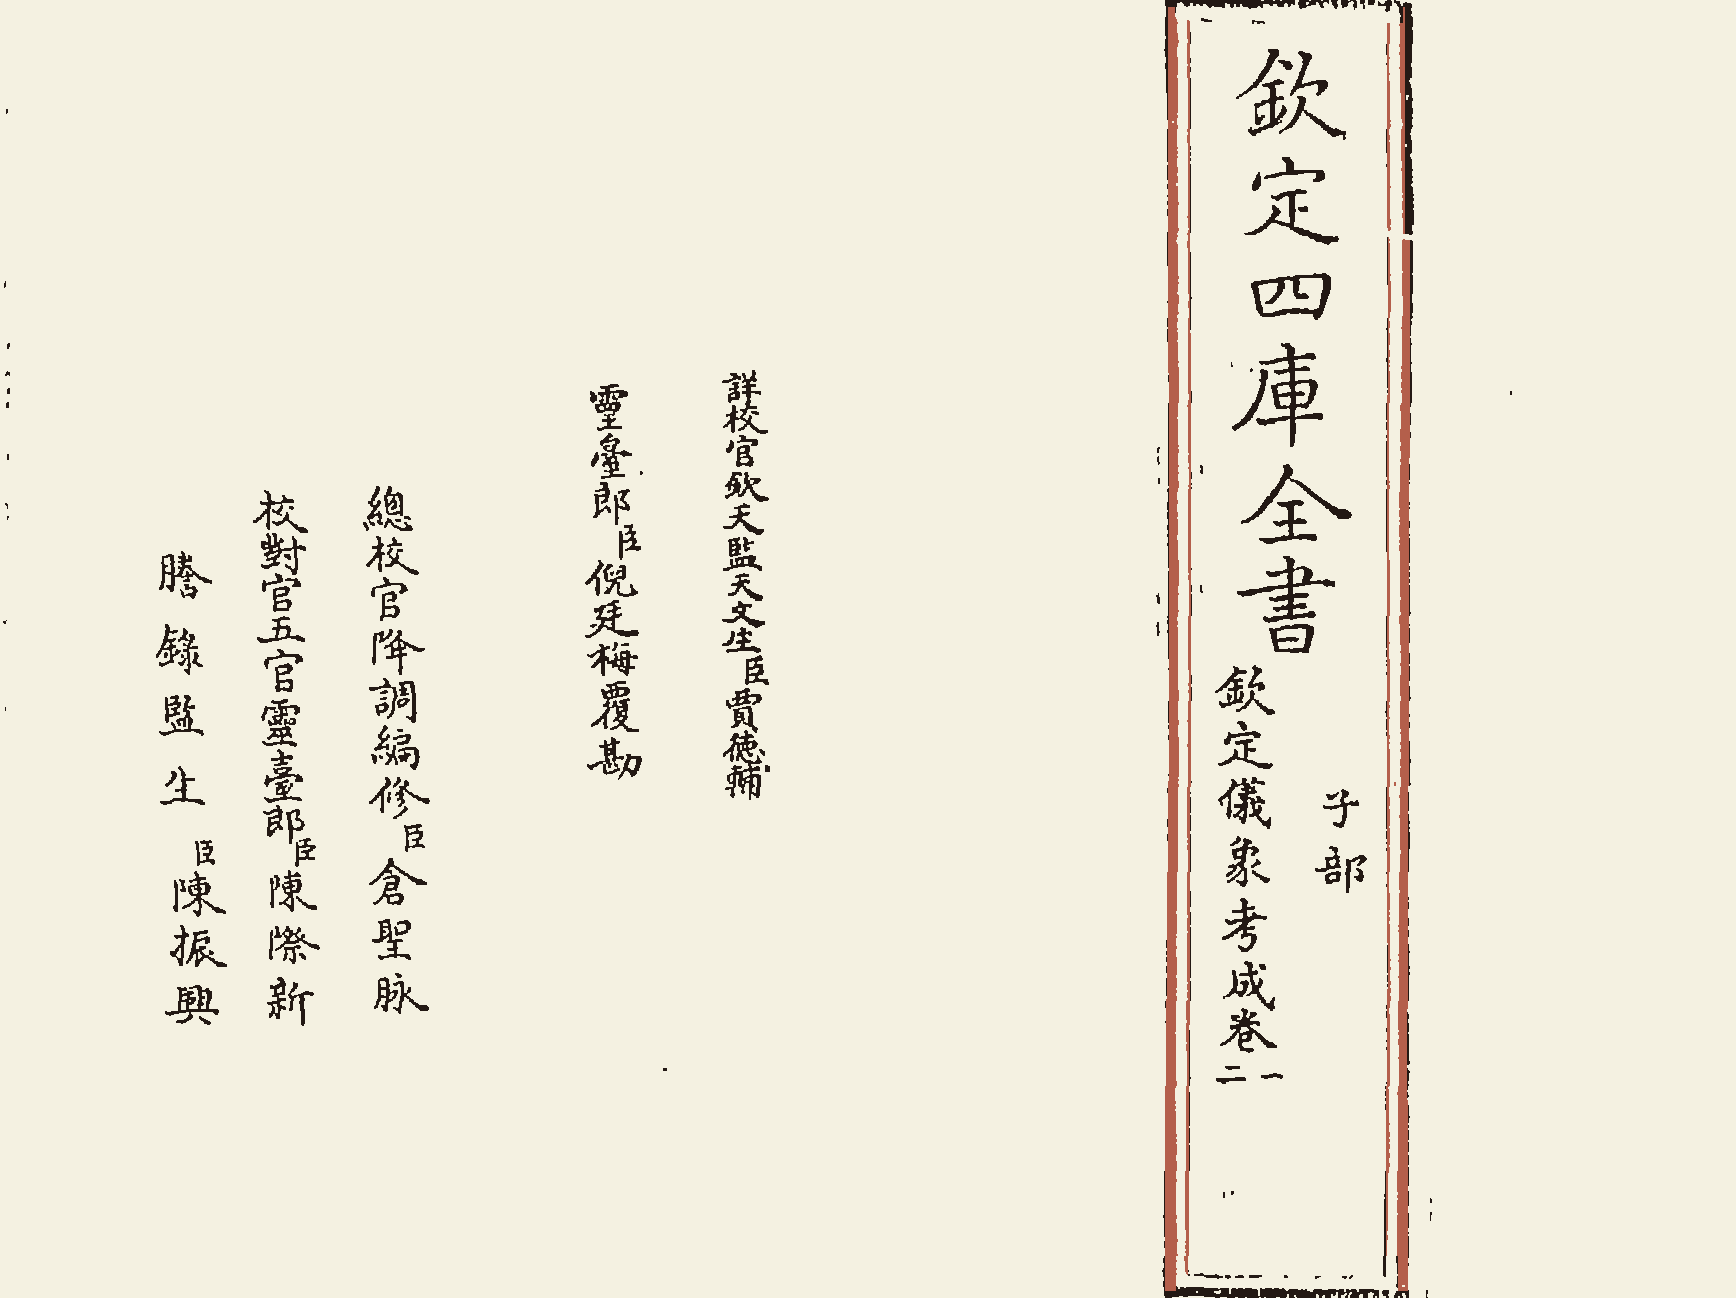
\includegraphics[width=\paperwidth,height=\paperheight,keepaspectratio]{img/0400.png}\clearpage
\begin{正文}
% ---- 册793 葉401 ----
\SetPageNumber{1}
欽定四庫全書\换行
欽定儀象考成卷一\换行
　恒星總紀\换行
　　三垣\换行
　　一十八宿\换行
　　恒星全圖\换行
　　赤道北恒星圖\换行
　　赤道南恒星圖\换行
\char"200B\relax\换行
\char"200B\relax\换行
\char"200B\relax\换行
\char"200B\relax\换行
\char"200B\relax\换行
\char"200B\relax\换行
\char"200B\relax\换行
\char"200B\relax
\par
% ---- 册793 葉404 ----
　　恒星總紀\换行
恒星即經星也以其有常不易故名經星\双列{\右小列{史記天官書}\左小列{紫宫房心權}}\换行
\双列{\右小列{衡咸池虚危列宿部星此天之五宫坐}\左小列{位也為經不移徙大小有差濶狹有常}}經星又各有經\换行
緯度故别之曰恒星其星官名數古今不同漢書天文\换行
志經星常宿中外官凡百一十八名積數七百八十三\换行
星晉志載呉太史令陳卓始列甘石巫咸三家星官著\换行
於圖録凡二百八十三官一千四百六十四星今皆不\换行
見原本隋丹元子歩天歌與陳卓數合後此言天官者\换行
皆以歩天歌為凖康熙十三年監臣南懐仁修儀象志\换行
星名與古同者總二百五十九座一千一百二十九星\换行
比歩天歌少二十四座三百三十五星又於有名常數\换行
之外増五百九十七星又多近南極星二十三座一百\换行
五十星近年以來累加測騐星官度數儀象志尚多未\换行
合又星之次第多不順序亦宜釐正於是逐星測量推\换行
其度數觀其形象序其次第著之於圖計三垣二十八\换行
宿星名與古同者總二百七十七座一千三百一十九
\par
% ---- 册793 葉405 ----
星比儀象志多十八座一百九十星與歩天歌為近其\换行
尤與古合者二十八宿次舍自古皆觜宿在前參宿在\换行
後其以何星作距古無明文唐書云古以參右肩為距\换行
失之太逺文獻通考載宋兩朝天文志云觜三星距西\换行
南星參十星距中星西第一星西法觜宿距中上星參\换行
宿亦距中西一星今按觜宿中上星在西南星前僅六\换行
分餘而西南星小中上星大則以中上星作距可也若\换行
參宿以中西一星作距星則觜宿之黄道度已在參宿\换行
後一度餘即赤道度亦在參宿後三十一分餘今依次\换行
順序以參宿中三星之東一星作距星則觜宿黄道度\换行
恒在參前一度弱與觜前參後之序合其餘諸座之星\换行
皆以次順序無凌躐顛倒之弊又於有名常數之外増\换行
一千六百一十四星近某座者即名某座増星依次分\换行
註方位以備稽考其近南極星二十三座一百五十星\换行
中國所不見仍依西測之舊共計恒星三百座三千八\换行
十三星編為總紀一卷庶星官名數古今不同及黄道
\par
% ---- 册793 葉408 ----
赤道所屬宫次皆展卷瞭然矣\换行
\char"200B\relax\换行
\char"200B\relax\换行
\char"200B\relax\换行
\char"200B\relax\换行
\char"200B\relax\换行
\char"200B\relax\换行
\char"200B\relax\换行
\char"200B\relax\换行
\char"200B\relax\换行
\char"200B\relax\换行
\char"200B\relax\换行
\char"200B\relax\换行
\char"200B\relax\换行
\char"200B\relax\换行
\char"200B\relax
\par
% ---- 册793 葉409 ----
紫微垣\换行
北極五星一太子二帝星三庶子四后宫五天樞外庶\换行
子増三星后宫増一星黄道在午未宫赤道在卯辰宫\换行
四輔四星外増一星黄道在未宫赤道在已午宫\换行
勾陳六星外増十星黄道在未申宫赤道在丑寅卯戌\换行
亥宫\换行
天皇大帝一星黄道在申宫赤道在亥宫\换行
天柱五星外増六星黄道在申酉宫赤道在子丑宫\换行
御女四星外増一星黄道在未申酉宫赤道在丑寅宫\换行
女史一星外増一星黄道在未宫赤道在寅宫\换行
柱史一星外増二星黄道在申宫赤道在丑宫\换行
尚書五星外増二星黄道在辰已午宫赤道在寅宫\换行
天床六星外増一星黄道在巳午宫赤道在寅卯宫\换行
大理二星外増一星黄道在未宫赤道在辰巳宫\换行
陰德二星外増一星黄道在未宫赤道在巳宫\换行
六甲六星外増一星黄道赤道俱在未申宫
\par
% ---- 册793 葉412 ----
五帝内座五星外増二星黄道在申宫赤道在酉戌宫\换行
華葢七星黄道在酉宫赤道在戌宫\换行
杠九星附華葢為一座外増一星黄道在申酉宫赤道\换行
在酉戌宫\换行
右垣墻七星一右樞二少尉三上輔四少輔五上衛六\换行
少衛七上丞外少尉増二星上輔増二星少輔増一星\换行
上衛増三星少衛増一星上丞増三星黄道在已午未\换行
申宫赤道在辰已午未申酉宫\换行
左垣墻八星一左樞二上宰三少宰四上弼五少弼六\换行
上衛七少衛八少丞外上衛増三星少衛増八星少丞\换行
増一星黄道在辰已酉宫赤道在戌亥子丑寅卯宫\换行
天乙一星黄道在已宫赤道在辰宫\换行
太乙一星黄道在午宫赤道在辰宫\换行
内厨二星外増二星黄道在午宫赤道在辰宫\换行
北斗七星一天樞二天璇三天璣四天權五玉衡六開\换行
陽七揺光外天樞増三星天璇増八星天權増三星開
\par
% ---- 册793 葉413 ----
陽増二星黄道在已午宫赤道在辰已宫\换行
輔一星附北斗為一座外増三星黄道在已宫赤道在\换行
辰宫\换行
天槍三星外増四星黄道在已宫赤道在卯宫\换行
元戈一星外増二星黄道在辰宫赤道在卯宫\换行
三公三星黄道在已宫赤道在辰宫\换行
相一星外増三星黄道在已宫赤道在辰宫\换行
天理四星外増一星黄道在午宫赤道在已宫\换行
太陽守一星外増一星黄道赤道俱在巳宫\换行
太尊一星黄道在午宫赤道在巳宫\换行
天牢六星外増二星黄道在巳午宫赤道在巳宫\换行
勢四星外増十六星黄道在午宫赤道在巳宫\换行
文昌六星外増八星黄道在午未宫赤道在午宫\换行
内階六星外増十星黄道在未宫赤道在午宫\换行
三師三星外増一星黄道在未宫赤道在午宫\换行
八榖八星外増三十四星黄道赤道俱在申宫
\par
% ---- 册793 葉416 ----
傳舍九星外増四星黄道在申酉宫赤道在酉戌亥宫\换行
天厨六星外増二星黄道在戌宫赤道在子丑宫\换行
天棓五星外増十星黄道赤道俱在寅宫\换行
　右共三十七座一百六十三星外増一百七十七星\换行
太微垣\换行
五帝座五星外増三星黄道赤道俱在巳宫\换行
太子一星黄道赤道俱在巳宫\换行
從官一星黄道赤道俱在巳宫\换行
幸臣一星黄道赤道俱在巳宫\换行
五諸侯五星外増七星黄道在辰巳宫赤道在辰宫\换行
九卿三星外増九星黄道赤道俱在辰宫\换行
三公三星黄道赤道俱在辰宫\换行
内屏四星外増六星黄道赤道俱在巳宫\换行
右垣墻五星一右執法二上將三次將四次相五上相\换行
外次相増三星上相増二星黄道赤道俱在巳宫\换行
左垣墻五星一左執法二上相三次相四次將五上將
\par
% ---- 册793 葉417 ----
外左執法增一星次相増一星次將増三星上將増二\换行
星黄道赤道俱在辰宫\换行
郎將一星外増二星黄道在巳宫赤道在辰宫\换行
郎位十五星外増三星黄道在巳宫赤道在辰巳宫\换行
常陳七星外増六星黄道在巳宫赤道在辰巳宫\换行
三台六星上台二星中台二星下台二星外上台増七\换行
星中台増三星下台増二星黄道在巳午未宫赤道在\换行
巳午宫\换行
虎賁一星黄道赤道俱在巳宫\换行
少微四星外增八星黄道在巳午宫赤道在巳宫\换行
長垣四星外増九星黄道在巳午宫赤道在巳宫\换行
靈臺三星外増八星黄道赤道俱在巳宫\换行
明堂三星外増六星黄道赤道俱在巳宫\换行
謁者一星外増二星黄道在巳宫赤道在辰宫\换行
　右共二十座七十八星外増九十三星\换行
天市垣
\par
% ---- 册793 葉420 ----
帝座一星黄道赤道俱在寅宫\换行
候一星外増五星黄道赤道俱在寅宫\换行
宦者四星外増五星黄道赤道俱在寅宫\换行
斗五星外増十四星黄道在寅卯宫赤道在寅宫\换行
斛四星外増三星黄道赤道俱在寅宫\换行
列肆二星外増四星黄道在寅卯宫赤道在寅宫\换行
車肆二星外増二星黄道赤道俱在寅宫\换行
市樓六星外増一星黄道赤道俱在寅宫\换行
宗正二星外増三星黄道赤道俱在寅宫\换行
宗人四星外増四星黄道赤道俱在寅宫\换行
宗二星黄道赤道俱在丑宫\换行
帛度二星外増三星黄道赤道俱在寅宫\换行
屠肆二星外増三星黄道赤道俱在丑寅宫\换行
右垣墻十一星一河中二河間三晉四鄭五周六秦七\换行
蜀八巴九梁十楚十一韓外河間増一星晉増三星周\换行
増十四星秦増一星蜀増二星巴増四星黄道赤道俱
\par
% ---- 册793 葉421 ----
在寅卯宫\换行
左垣墻十一星一魏二趙三九河四中山五齊六呉越\换行
七徐八東海九燕十南海十一宋外魏増八星趙増三\换行
星九河増一星中山増七星齊増八星呉越増七星徐\换行
増四星東海増四星宋増二星黄道赤道俱在丑寅宫\换行
天紀九星外増十四星黄道在寅卯宫赤道在寅宫\换行
女牀三星黄道赤道俱在寅宫\换行
貫索九星外増十三星黄道赤道俱在卯宫\换行
七公七星外増十六星黄道在卯辰宫赤道在寅卯宫\换行
　右共十九座八十七星外増一百五十九星\换行
角宿\换行
角宿二星外増十五星黄道赤道俱在辰宫\换行
平道二星黄道赤道俱在辰宫\换行
天田二星外増六星黄道赤道俱在辰宫\换行
周鼎三星黄道在辰巳宫赤道在辰宫\换行
進賢一星外増九星黄道赤道俱在辰宫
\par
% ---- 册793 葉424 ----
天門二星外増十一星黄道赤道俱在辰宫\换行
平二星外増三星黄道在卯辰宫赤道在辰宫\换行
庫樓十星外増一星黄道赤道俱在卯辰宫\换行
柱十一星黄道赤道俱在卯辰宫\换行
衡四星黄道在卯宫赤道在辰宫\换行
南門二星外増二星黄道在卯宫赤道在卯辰宫\换行
　右共十一座四十一星外増四十七星\换行
亢宿\换行
亢宿四星外増十二星黄道在卯宫赤道在卯辰宫\换行
大角一星外増一星黄道在辰宫赤道在卯宫\换行
右攝提三星外増三星黄道赤道俱在辰宫\换行
左攝提三星外増三星黄道在卯辰宫赤道在卯宫\换行
折威七星外増六星黄道赤道俱在卯宫\换行
頓頑二星外増一星黄道赤道俱在卯宫\换行
陽門二星黄道赤道俱在卯宫\换行
　右共七座二十二星外増二十六星
\par
% ---- 册793 葉425 ----
氐宿\换行
氐宿四星外増二十九星黄道赤道俱在卯宫\换行
亢池四星黄道在辰宫赤道在卯辰宫\换行
帝席三星外増一星黄道赤道俱在辰宫\换行
梗河三星外増五星黄道在卯辰宫赤道在卯宫\换行
招揺一星黄道在辰宫赤道在卯宫\换行
天乳一星外増三星黄道赤道俱在卯宫\换行
天輻二星外増一星黄道赤道俱在卯宫\换行
陣車三星外増二星黄道赤道俱在卯宫\换行
騎官十星黄道赤道俱在卯宫\换行
車騎三星黄道赤道俱在卯宫\换行
將軍一星黄道赤道俱在卯宫\换行
　右共十一座三十五星外増四十一星\换行
房宿\换行
房宿四星外増六星黄道赤道俱在卯宫\换行
鈎鈐二星附房宿為一座黄道在寅宫赤道在卯宫
\par
% ---- 册793 葉428 ----
鍵閉一星黄道在卯宫赤道在寅宫\换行
罰三星外増三星黄道在卯宫赤道在寅卯宫\换行
西咸四星外増二星黄道赤道俱在卯宫\换行
東咸四星外増一星黄道赤道俱在寅宫\换行
日一星外増一星黄道赤道俱在卯宫\换行
從官二星外増一星黄道赤道俱在卯宫\换行
　右共七座二十一星外増十四星\换行
心宿\换行
心宿三星外増八星黄道赤道俱在寅宫\换行
積卒二星黄道在寅宫赤道在卯宫\换行
　右共二座五星外増八星\换行
尾宿\换行
尾宿九星外増一星黄道赤道俱在寅宫\换行
神宫一星附尾宿為一座黄道赤道俱在寅宫\换行
天江四星外増十一星黄道赤道俱在寅宫\换行
傅説一星黄道赤道俱在寅宫
\par
% ---- 册793 葉429 ----
魚一星黄道赤道俱在寅宫\换行
龜五星黄道赤道俱在寅宫\换行
　右共五座二十一星外増十二星\换行
箕宿\换行
箕宿四星黄道赤道俱在丑寅宫\换行
糠一星黄道赤道俱在寅宫\换行
杵三星外増一星黄道赤道俱在寅宫\换行
　右共三座八星外増一星\换行
斗宿\换行
斗宿六星外増四星黄道赤道俱在丑寅宫\换行
天籥八星外増四星黄道赤道俱在寅宫\换行
天弁九星外増五星黄道赤道俱在丑宫\换行
建六星外増八星黄道赤道俱在丑宫\换行
天雞二星外増三星黄道赤道俱在丑宫\换行
狗二星外増六星黄道赤道俱在丑宫\换行
狗國四星黄道赤道俱在丑宫
\par
% ---- 册793 葉432 ----
天淵三星黄道赤道俱在丑宫\换行
農丈人一星黄道赤道俱在丑宫\换行
鼈十一星黄道赤道俱在丑宫\换行
　右共十座五十二星外増三十星\换行
牛宿\换行
牛宿六星外増九星黄道赤道俱在子丑宫\换行
天桴四星外増二星黄道在子丑宫赤道在丑宫\换行
河鼓三星外増九星黄道赤道俱在丑宫\换行
右旗九星外増十二星黄道赤道俱在丑宫\换行
左旗九星外増二十九星黄道赤道俱在子丑宫\换行
織女三星外増四星黄道赤道俱在丑宫\换行
漸臺四星外増六星黄道赤道俱在丑宫\换行
輦道五星外増九星黄道在子丑宫赤道在丑宫\换行
羅堰三星外增一星黄道赤道俱在子宫\换行
天田四星黄道赤道俱在子宫\换行
九坎四星黄道赤道俱在子宫
\par
% ---- 册793 葉433 ----
　右共十一座五十四星外増八十一星\换行
女宿\换行
女宿四星外増五星黄道赤道俱在子宫\换行
離珠四星外増一星黄道赤道俱在子宫\换行
敗𤓰五星外増三星黄道赤道俱在子宫\换行
瓠𤓰五星外増五星黄道赤道俱在子宫\换行
天津九星外増三十八星黄道在亥子宫赤道在子丑\换行
宫\换行
奚仲四星外増七星黄道在子宫赤道在丑宫\换行
扶筐七星外増四星黄道在子丑宫赤道在丑宫\换行
十二國十六星周二星秦二星代二星趙二星越一星\换行
齊一星楚一星鄭一星魏一星韓一星晉一星燕一星\换行
外代増二星黄道赤道俱在子宫\换行
　右共八座五十四星外増六十五星\换行
虚宿\换行
虚宿二星外増八星黄道赤道俱在子宫
\par
% ---- 册793 葉436 ----
司命二星黄道赤道俱在子宫\换行
司禄二星外増二星黄道赤道俱在子宫\换行
司危二星黄道赤道俱在子宫\换行
司非二星外増二星黄道赤道俱在子宫\换行
哭二星外増四星黄道赤道俱在子宫\换行
泣二星外増二星黄道在亥子宫赤道在亥宫\换行
離瑜三星外増三星黄道赤道俱在子宫\换行
天壘城十三星黄道赤道俱在子宫\换行
敗臼四星外増一星黄道在子宫赤道在亥子宫\换行
　右共十座三十四星外増二十二星\换行
危宿\换行
危宿三星外増十一星黄道在亥子宫赤道在子宫\换行
墳墓四星附危宿為一座外増四星黄道赤道俱在亥\换行
宫\换行
葢屋二星黄道赤道俱在子宫\换行
虚梁四星黄道赤道俱在亥宫
\par
% ---- 册793 葉437 ----
天錢五星外増四星黄道赤道俱在子宫\换行
人四星外増四星黄道在亥子宫赤道在子宫\换行
杵三星外増二星黄道在亥宫赤道在亥子宫\换行
臼四星外増五星黄道在亥宫赤道在亥子宫\换行
車府七星外増十九星黄道在戌亥宫赤道在亥子宫\换行
造父五星外増五星黄道在戌宫赤道在亥子宫\换行
天鉤九星外増十六星黄道在酉戌宫赤道在亥子宫\换行
　右共十座五十星外増七十星\换行
室宿\换行
室宿二星外増七星黄道赤道俱在亥宫\换行
離宫六星附室宿為一座外増八星黄道赤道俱在亥\换行
宫\换行
螣蛇二十二星外増十四星黄道在戌亥宫赤道在亥\换行
子宫\换行
雷電六星外増八星黄道赤道俱在亥宫\换行
土公吏二星黄道赤道俱在亥宫
\par
% ---- 册793 葉440 ----
壘壁陣十二星外増七星黄道赤道俱在亥子宫\换行
羽林軍四十五星黄道赤道俱在亥子宫\换行
天綱一星黄道在子宫赤道在亥宫\换行
北落師門一星黄道赤道俱在亥宫\换行
鈇鉞三星外増二星黄道赤道俱在亥宫\换行
八魁六星黄道在亥宫赤道在戌亥宫\换行
　右共十座一百零六星外増四十六星\换行
壁宿\换行
壁宿二星外増二十三星黄道在戌宫赤道在戌亥宫\换行
天廐三星外増一星黄道赤道俱在戌宫\换行
土公二星外増十一星黄道在戌宫赤道在戌亥宫\换行
霹𩆝五星外増八星黄道赤道俱在亥宫\换行
雲雨四星外増九星黄道赤道俱在亥宫\换行
鈇鑕五星黄道赤道俱在戌宫\换行
　右共六座二十一星外増五十二星\换行
奎宿
\par
% ---- 册793 葉441 ----
奎宿十六星外増二十二星黄道赤道俱在戌宫\换行
王良五星外増五星黄道在酉宫赤道在戌亥宫\换行
䇿一星黄道在酉宫赤道在戌宫\换行
附路一星黄道在酉宫赤道在戌宫\换行
軍南門一星黄道在酉宫赤道在戌宫\换行
閣道六星外増五星黄道赤道俱在酉戌宫\换行
外屏七星外増十五星黄道赤道俱在戌宫\换行
天溷四星外増六星黄道赤道俱在戌宫\换行
土司空一星黄道在亥宫赤道在戌宫\换行
　右共九座四十二星外増五十三星\换行
婁宿\换行
婁宿三星外増十五星黄道在酉戌宫赤道在戌宫\换行
天大將軍十一星外増十六星黄道在酉宫赤道在酉\换行
戌宫\换行
右更五星外増五星黄道赤道俱在戌宫\换行
左更五星外増七星黄道赤道俱在酉宫
\par
% ---- 册793 葉444 ----
天倉六星外増十八星黄道在戌亥宫赤道在戌宫\换行
天庾三星外増三星黄道在戌宫赤道在酉戌宫\换行
　右共六座三十三星外増六十四星\换行
胃宿\换行
胃宿三星外増五星黄道赤道俱在酉宫\换行
大陵八星外増二十星黄道赤道俱在酉宫\换行
積尸一星黄道赤道俱在酉宫\换行
天船九星外増九星黄道在申酉宫赤道在酉宫\换行
積水一星外増一星黄道在申宫赤道在酉宫\换行
天廩四星外増二星黄道赤道俱在酉宫\换行
天囷十三星外増二十星黄道赤道俱在酉戌宫\换行
　右共七座三十九星外増五十七星\换行
昴宿\换行
昴宿七星外増五星黄道赤道俱在酉宫\换行
天阿一星黄道赤道俱在酉宫\换行
月一星外増一星黄道赤道俱在酉宫
\par
% ---- 册793 葉445 ----
卷舌六星外増六星黄道在申酉宫赤道在酉宫\换行
天讒一星黄道赤道俱在酉宫\换行
礪石四星黄道在申宫赤道在申酉宫\换行
天陰五星外増四星黄道赤道俱在酉宫\换行
蒭藁六星外増五星黄道在戌宫赤道在酉宫\换行
天苑十六星外増十六星黄道在酉戌宫赤道在酉宫\换行
　右共九座四十七星外増三十七星\换行
畢宿\换行
畢宿八星外増十三星黄道赤道俱在申酉宫\换行
附耳一星附畢宿為一座外増一星黄道赤道俱在申\换行
宫\换行
天街二星外増四星黄道赤道俱在申宫\换行
天髙四星外増四星黄道赤道俱在申宫\换行
諸王六星外増四星黄道赤道俱在申宫\换行
五車五星外増十八星黄道赤道俱在申宫\换行
柱九星黄道赤道俱在申宫
\par
% ---- 册793 葉448 ----
咸池三星黄道赤道俱在申宫\换行
天潢五星外増二星黄道赤道俱在申宫\换行
天闗一星外増六星黄道赤道俱在申宫\换行
天節八星黄道赤道俱在申宫\换行
九州殊口六星外増十星黄道赤道俱在申酉宫\换行
參旗九星外増十一星黄道赤道俱在申宫\换行
九斿九星外増五星黄道赤道俱在申宫\换行
天園十三星外増六星黄道在酉戌亥宫赤道在申酉\换行
戌宫\换行
　右共十四座八十九星外増八十四星\换行
觜宿\换行
觜宿三星黄道赤道俱在申宫\换行
司怪四星外増六星黄道赤道俱在申宫\换行
座旗九星外増十一星黄道赤道俱在未宫\换行
　右共三座十六星外増十七星\换行
參宿
\par
% ---- 册793 葉449 ----
參宿七星外増三十七星黄道赤道俱在申宫\换行
伐三星附參宿為一座外増二星黄道赤道俱在申宫\换行
玉井四星外増二星黄道赤道俱在申宫\换行
軍井四星外増一星黄道赤道俱在申宫\换行
屏二星黄道赤道俱在申宫\换行
厠四星外増七星黄道赤道俱在申宫\换行
屎一星黄道赤道俱在申宫\换行
　右共六座二十五星外増四十九星\换行
井宿\换行
井宿八星外増十七星黄道赤道俱在未宫\换行
龯一星附井宿為一座外増一星黄道赤道俱在申宫\换行
水府四星外増八星黄道赤道俱在未申宫\换行
天罇三星外増九星黄道赤道俱在未宫\换行
五諸侯五星外増五星黄道赤道俱在未宫\换行
北河三星外増四星黄道赤道俱在未宫\换行
積水一星黄道赤道俱在未宫
\par
% ---- 册793 葉452 ----
積薪一星外増三星黄道赤道俱在未宫\换行
水位四星外増十一星黄道赤道俱在未宫\换行
南河三星外増十星黄道赤道俱在未宫\换行
四瀆四星外増六星黄道赤道俱在未宫\换行
闕邱二星外増七星黄道赤道俱在未宫\换行
軍市六星外増五星黄道赤道俱在未宫\换行
野雞一星黄道赤道俱在未宫\换行
天狼一星外増五星黄道赤道俱在未宫\换行
丈人二星黄道赤道俱在申宫\换行
子二星外増一星黄道赤道俱在申宫\换行
孫二星外増四星黄道赤道俱在未申宫\换行
老人一星外増四星黄道赤道俱在未宫\换行
弧矢九星外増二十四星黄道在午未宫赤道在未宫\换行
　右共十九座六十三星外増一百二十四星\换行
鬼宿\换行
鬼宿四星外増十八星黄道赤道俱在午宫
\par
% ---- 册793 葉453 ----
積尸氣一星外増三星黄道赤道俱在午宫\换行
爟四星外増十一星黄道赤道俱在未宫\换行
外厨六星外増十七星黄道赤道俱在午宫\换行
天記一星外増二星黄道在己宫赤道在午宫\换行
天狗七星黄道在巳午宫赤道在午宫\换行
天社六星外増五星黄道在辰巳午宫赤道在午宫\换行
　右共六座二十九星外増五十七星\换行
柳宿\换行
柳宿八星外増十星黄道赤道俱在午宫\换行
酒旗三星外増五星黄道赤道俱在午宫\换行
　右共二座十一星外増十五星\换行
星宿\换行
星宿七星外増十五星黄道赤道俱在午宫\换行
天相三星外増十二星黄道在己宫赤道在己午宫\换行
軒轅十七星外増五十七星黄道赤道俱在己午宫\换行
内平四星外増十一星黄道在午宫赤道在己午宫
\par
% ---- 册793 葉456 ----
　右共四座三十一星外増九十五星\换行
張宿\换行
張宿六星外増四星黄道赤道俱在己午宫\换行
　右一座六星外増四星\换行
翼宿\换行
翼宿二十二星外增七星黄道在辰己宫赤道在己宫\换行
　右一座二十二星外増七星\换行
軫宿\换行
軫宿四星外増五星黄道在辰宫赤道在辰己宫\换行
右轄一星附軫宿為一座黄道在辰宫赤道在己宫\换行
左轄一星附軫宿為一座黄道赤道俱在辰宫\换行
長沙一星附軫宿為一座黄道赤道俱在辰宫\换行
青邱七星外増三星黄道在辰宫赤道在己宫\换行
　右共二座十四星外増八星\换行
　總計三垣二十八宿共二百七十七座一千三百一\换行
　十九星外増一千六百一十四星按天文歩天歌角
\par
% ---- 册793 葉457 ----
　宿内柱十五星今少四星氐宿内亢池六星今少二\换行
　星騎官二十七星今少十七星心宿内積卒十二星\换行
　今少十星斗宿内天淵十星今少七星鼈十四星今\换行
　少三星牛宿内天田九星今少五星九坎九星今少\换行
　五星女宿内離珠五星今少一星危宿内天錢十星\换行
　今少五星人五星今少一星室宿内八魁九星今少\换行
　三星壁宿内天廐十星今少七星奎宿内天溷七星\换行
　今少三星畢宿内九州殊口九星今少三星井宿内\换行
　軍市十三星今少七星共少八十三星星宿内天稷\换行
　五星張宿内天廟十四星翼宿内東甌五星軫宿内\换行
　軍門二星土司空四星器府三十二星共六座六十\换行
　二星今無\换行
近南極星\换行
海山六星外増二星黄道在卯辰宫赤道在己宫\换行
十字四星黄道在卯宫赤道在辰宫\换行
馬尾三星黄道在辰宫赤道在辰己宫
\par
% ---- 册793 葉460 ----
馬腹三星黄道在卯宫赤道在辰宫\换行
蜜蜂四星黄道在卯宫赤道在辰宫\换行
三角形三星外増四星黄道在寅宫赤道在寅卯宫\换行
異雀九星黄道在寅宫赤道在寅卯辰宫\换行
孔雀十一星外増四星黄道在丑寅宫赤道在子丑寅\换行
宫\换行
波斯十一星黄道赤道俱在子丑宫\换行
蛇尾四星黄道在丑宫赤道在戌亥子宫\换行
蛇腹四星黄道在亥子宫赤道在酉戌宫\换行
蛇首二星黄道在亥宫赤道在酉戌宫\换行
鳥喙七星外増一星黄道在子宫赤道在戌亥宫\换行
鶴十二星外増二星黄道在子宫赤道在亥子宫\换行
火鳥十星外増一星黄道在亥子宫赤道在戌亥宫\换行
水委三星黄道在亥宫赤道在戌宫\换行
附白二星黄道在子宫赤道在酉宫\换行
夾白二星黄道在戌亥宫赤道在申酉宫
\par
% ---- 册793 葉461 ----
金魚五星外増一星黄道在寅酉戌宫赤道在未申宫\换行
海石五星外増三星黄道在辰己宫赤道在午宫\换行
飛魚六星黄道在卯辰宫赤道在午未宫\换行
南船五星外増一星黄道在卯辰宫赤道在己午宫\换行
小斗九星外増一星黄道在寅卯宫赤道在辰巳午未\换行
宫\换行
　右共二十三座一百三十星外増二十星古無\换行
\char"200B\relax\换行
\char"200B\relax\换行
\char"200B\relax\换行
\char"200B\relax\换行
\char"200B\relax\换行
\char"200B\relax\换行
\char"200B\relax\换行
\char"200B\relax\换行
\char"200B\relax
\par
% ---- 册793 葉464 ----
　　恒星全圖\换行
唐書天文志葢天之説一行削篾為度徑一分其厚半\换行
之長與圖等穴其正中植鍼為樞令可環運自中樞之\换行
外均刻百四十七度全度之末旋為外規規外大半度\换行
再旋為重規以均賦周天度分又距極樞九十一度少\换行
半旋為赤道𢃄天之紘距極三十五度旋為内規乃歩\换行
冬至日躔所在以正辰次之中以立宿距按渾儀所測\换行
甘石巫咸衆星明者皆以篾横考入宿距縱考去極度\换行
而後圖之其赤道外衆星踈宻之狀與仰視小殊者由\换行
渾儀去南極漸近其度益狹而葢圖漸逺其度益廣使\换行
然若考其去極入宿度數移之於渾天則一也又赤道\换行
内外其廣狹不均若就二至出入赤道二十四度以規\换行
度之則二分所交不得其正自二分黄赤道交以規度\换行
之則二至距極度數不得其正當求黄赤分至之中均\换行
刻為七十二限據每黄道差數以篾度量而識之然後\换行
規為黄道則周天咸得其正矣今按渾天係圓體圖之
\par
% ---- 册793 葉465 ----
於平面止見其半故渾天不可圖葢天圖以北極為中\换行
心乃見星座全象然其内外二規亦猶是渾天之法也\换行
渾天家以北極出地常見不隠謂之上規南極入地常\换行
隠不見謂之下規一行葢天圖以三十五度為内規即\换行
上規之度也\双列{\右小列{北極出地}\左小列{三十五度}}一百四十七度為外規即北極\换行
距下規之度也\双列{\右小列{古法周天三百六十五度四分度之一}\左小列{則北極距南極為一百八十二度有竒}}\换行
\双列{\右小列{除南極入地三十五度}\左小列{有竒餘一百四十七度}}今法周天三百六十度赤道距\换行
南北極各九十度京師北極出地四十度故以四十度\换行
為内規中國幅隕南至北極出地二十度則北極距下\换行
規一百六十度故以一百六十度為外規其餘悉如一\换行
行之法依新測恒星赤道經緯度著之於圖仍用赤黄\换行
黒三色以存三家之舊又以赤道南北分為二圖則北\换行
極出地二十度以南所見之星座無不備具雖中天所\换行
見星座横分為二然赤道以南其度漸狹可以補葢天\换行
星度益廣之失合觀三圖則懸象著明躔離攸次星之\换行
隠見天漢昭回庶幾無遺憾矣
\par
\end{正文}\clearpage
\嵌图{141.61pt}{202.05pt}{848.55pt}{585.69pt}{img/0470.png}
\begin{正文}
% ---- 册793 葉470 图版 ----
\SetPageNumber{34}
\插图页
\char"200B\relax\换行
\char"200B\relax\换行
\char"200B\relax\换行
\char"200B\relax\换行
\char"200B\relax\换行
\char"200B\relax\换行
\char"200B\relax\换行
\char"200B\relax\换行
\char"200B\relax\换行
\char"200B\relax\换行
\char"200B\relax\换行
\char"200B\relax\换行
\char"200B\relax\换行
\char"200B\relax\换行
\char"200B\relax\换行
\char"200B\relax
\恢复丝栏\par
\end{正文}\clearpage
\嵌图{145.79pt}{200.67pt}{840.19pt}{588.45pt}{img/0474.png}
\begin{正文}
% ---- 册793 葉474 图版 ----
\SetPageNumber{35}
\插图页
\char"200B\relax\换行
\char"200B\relax\换行
\char"200B\relax\换行
\char"200B\relax\换行
\char"200B\relax\换行
\char"200B\relax\换行
\char"200B\relax\换行
\char"200B\relax\换行
\char"200B\relax\换行
\char"200B\relax\换行
\char"200B\relax\换行
\char"200B\relax\换行
\char"200B\relax\换行
\char"200B\relax\换行
\char"200B\relax\换行
\char"200B\relax
\恢复丝栏\par
\end{正文}\clearpage
\嵌图{147.13pt}{204.95pt}{837.49pt}{579.89pt}{img/0478.png}
\begin{正文}
% ---- 册793 葉478 图版 ----
\SetPageNumber{36}
\插图页
\char"200B\relax\换行
\char"200B\relax\换行
\char"200B\relax\换行
\char"200B\relax\换行
\char"200B\relax\换行
\char"200B\relax\换行
\char"200B\relax\换行
\char"200B\relax\换行
\char"200B\relax\换行
\char"200B\relax\换行
\char"200B\relax\换行
\char"200B\relax\换行
\char"200B\relax\换行
\char"200B\relax\换行
\char"200B\relax\换行
\char"200B\relax
\恢复丝栏\par

% ======== 卷二（8行21字）========
\par\end{正文}\clearpage
\chapter*{欽定儀象考成卷二}
\begin{正文}
% ---- 册793 葉480 ----
\SetPageNumber{1}
欽定四庫全書\换行
欽定儀象考成卷二\换行
　恒星黄道經緯度表一\换行
　　黄道星紀宫\双列{\右小列{赤道度附}\左小列{}}\换行
\char"200B\relax\换行
\char"200B\relax\换行
\char"200B\relax\换行
\char"200B\relax\换行
\char"200B\relax\换行
\char"200B\relax\换行
\char"200B\relax\换行
\char"200B\relax\换行
\char"200B\relax\换行
\char"200B\relax\换行
\char"200B\relax\换行
\char"200B\relax
\par
% ---- 册793 葉481 ----
　　恒星黄赤經緯度表\换行
恒星布列周天古有去極入宿度數入宿即經度也去\换行
極即緯度也然黄道度與赤道度不同嵗差亦異葢黄\换行
道以黄極為樞赤道以赤極為樞兩道兩極各相距二\换行
十三度半故星在兩極之間者黄道屬未宫赤道則屬\换行
丑宫星在兩道之間者黄道屬緯南赤道則屬緯北此\换行
黄赤不同之極致也恒星循黄道東行每年五十一秒\换行
緯度終古不改而經度之差有常赤道與黄道斜交分\换行
至前後南北逺近其差不等兩極之間在黄道為差而\换行
東在赤道為差而西兩交之際黄道南者差而入赤道\换行
北黄道北者差而出赤道南此嵗差不同之極致也今\换行
以乾隆九年甲子恒星黄赤經緯度依黄道次序列恒\换行
星黄道經緯度表而以赤道經緯附之依赤道次序列\换行
恒星赤道經緯度表而以黄道經緯附之各將赤道嵗\换行
差列於其下黄道以便推算赤道以便測量厯象之用\换行
於斯備矣
\par
\end{正文}\clearpage
\嵌图{142.64pt}{198.13pt}{846.47pt}{593.52pt}{img/0484.png}
\begin{正文}
% ---- 册793 葉484 图版 ----
\SetPageNumber{3}
\插图页
\char"200B\relax\换行
\char"200B\relax\换行
\char"200B\relax\换行
\char"200B\relax\换行
\char"200B\relax\换行
\char"200B\relax\换行
\char"200B\relax\换行
\char"200B\relax\换行
\char"200B\relax\换行
\char"200B\relax\换行
\char"200B\relax\换行
\char"200B\relax\换行
\char"200B\relax\换行
\char"200B\relax\换行
\char"200B\relax\换行
\char"200B\relax
\恢复丝栏\par
\end{正文}\clearpage
\嵌图{142.64pt}{198.61pt}{846.47pt}{592.57pt}{img/0485.png}
\begin{正文}
% ---- 册793 葉485 图版 ----
\SetPageNumber{4}
\插图页
\char"200B\relax\换行
\char"200B\relax\换行
\char"200B\relax\换行
\char"200B\relax\换行
\char"200B\relax\换行
\char"200B\relax\换行
\char"200B\relax\换行
\char"200B\relax\换行
\char"200B\relax\换行
\char"200B\relax\换行
\char"200B\relax\换行
\char"200B\relax\换行
\char"200B\relax\换行
\char"200B\relax\换行
\char"200B\relax\换行
\char"200B\relax
\恢复丝栏\par
\end{正文}\clearpage
\嵌图{144.63pt}{200.02pt}{842.50pt}{589.74pt}{img/0488.png}
\begin{正文}
% ---- 册793 葉488 图版 ----
\SetPageNumber{5}
\插图页
\char"200B\relax\换行
\char"200B\relax\换行
\char"200B\relax\换行
\char"200B\relax\换行
\char"200B\relax\换行
\char"200B\relax\换行
\char"200B\relax\换行
\char"200B\relax\换行
\char"200B\relax\换行
\char"200B\relax\换行
\char"200B\relax\换行
\char"200B\relax\换行
\char"200B\relax\换行
\char"200B\relax\换行
\char"200B\relax\换行
\char"200B\relax
\恢复丝栏\par
\end{正文}\clearpage
\嵌图{144.63pt}{200.00pt}{842.50pt}{589.78pt}{img/0489.png}
\begin{正文}
% ---- 册793 葉489 图版 ----
\SetPageNumber{6}
\插图页
\char"200B\relax\换行
\char"200B\relax\换行
\char"200B\relax\换行
\char"200B\relax\换行
\char"200B\relax\换行
\char"200B\relax\换行
\char"200B\relax\换行
\char"200B\relax\换行
\char"200B\relax\换行
\char"200B\relax\换行
\char"200B\relax\换行
\char"200B\relax\换行
\char"200B\relax\换行
\char"200B\relax\换行
\char"200B\relax\换行
\char"200B\relax
\恢复丝栏\par
\end{正文}\clearpage
\嵌图{148.54pt}{198.57pt}{834.68pt}{592.64pt}{img/0492.png}
\begin{正文}
% ---- 册793 葉492 图版 ----
\SetPageNumber{7}
\插图页
\char"200B\relax\换行
\char"200B\relax\换行
\char"200B\relax\换行
\char"200B\relax\换行
\char"200B\relax\换行
\char"200B\relax\换行
\char"200B\relax\换行
\char"200B\relax\换行
\char"200B\relax\换行
\char"200B\relax\换行
\char"200B\relax\换行
\char"200B\relax\换行
\char"200B\relax\换行
\char"200B\relax\换行
\char"200B\relax\换行
\char"200B\relax
\恢复丝栏\par
\end{正文}\clearpage
\嵌图{148.54pt}{197.60pt}{834.68pt}{594.58pt}{img/0493.png}
\begin{正文}
% ---- 册793 葉493 图版 ----
\SetPageNumber{8}
\插图页
\char"200B\relax\换行
\char"200B\relax\换行
\char"200B\relax\换行
\char"200B\relax\换行
\char"200B\relax\换行
\char"200B\relax\换行
\char"200B\relax\换行
\char"200B\relax\换行
\char"200B\relax\换行
\char"200B\relax\换行
\char"200B\relax\换行
\char"200B\relax\换行
\char"200B\relax\换行
\char"200B\relax\换行
\char"200B\relax\换行
\char"200B\relax
\恢复丝栏\par
\end{正文}\clearpage
\嵌图{148.61pt}{200.04pt}{834.55pt}{589.71pt}{img/0496.png}
\begin{正文}
% ---- 册793 葉496 图版 ----
\SetPageNumber{9}
\插图页
\char"200B\relax\换行
\char"200B\relax\换行
\char"200B\relax\换行
\char"200B\relax\换行
\char"200B\relax\换行
\char"200B\relax\换行
\char"200B\relax\换行
\char"200B\relax\换行
\char"200B\relax\换行
\char"200B\relax\换行
\char"200B\relax\换行
\char"200B\relax\换行
\char"200B\relax\换行
\char"200B\relax\换行
\char"200B\relax\换行
\char"200B\relax
\恢复丝栏\par
\end{正文}\clearpage
\嵌图{146.62pt}{199.56pt}{838.53pt}{590.67pt}{img/0497.png}
\begin{正文}
% ---- 册793 葉497 图版 ----
\SetPageNumber{10}
\插图页
\char"200B\relax\换行
\char"200B\relax\换行
\char"200B\relax\换行
\char"200B\relax\换行
\char"200B\relax\换行
\char"200B\relax\换行
\char"200B\relax\换行
\char"200B\relax\换行
\char"200B\relax\换行
\char"200B\relax\换行
\char"200B\relax\换行
\char"200B\relax\换行
\char"200B\relax\换行
\char"200B\relax\换行
\char"200B\relax\换行
\char"200B\relax
\恢复丝栏\par
\end{正文}\clearpage
\嵌图{142.64pt}{197.65pt}{846.47pt}{594.50pt}{img/0500.png}
\begin{正文}
% ---- 册793 葉500 图版 ----
\SetPageNumber{11}
\插图页
\char"200B\relax\换行
\char"200B\relax\换行
\char"200B\relax\换行
\char"200B\relax\换行
\char"200B\relax\换行
\char"200B\relax\换行
\char"200B\relax\换行
\char"200B\relax\换行
\char"200B\relax\换行
\char"200B\relax\换行
\char"200B\relax\换行
\char"200B\relax\换行
\char"200B\relax\换行
\char"200B\relax\换行
\char"200B\relax\换行
\char"200B\relax
\恢复丝栏\par
\end{正文}\clearpage
\嵌图{144.63pt}{199.49pt}{842.50pt}{590.81pt}{img/0501.png}
\begin{正文}
% ---- 册793 葉501 图版 ----
\SetPageNumber{12}
\插图页
\char"200B\relax\换行
\char"200B\relax\换行
\char"200B\relax\换行
\char"200B\relax\换行
\char"200B\relax\换行
\char"200B\relax\换行
\char"200B\relax\换行
\char"200B\relax\换行
\char"200B\relax\换行
\char"200B\relax\换行
\char"200B\relax\换行
\char"200B\relax\换行
\char"200B\relax\换行
\char"200B\relax\换行
\char"200B\relax\换行
\char"200B\relax
\恢复丝栏\par
\end{正文}\clearpage
\嵌图{144.68pt}{202.35pt}{842.41pt}{585.10pt}{img/0504.png}
\begin{正文}
% ---- 册793 葉504 图版 ----
\SetPageNumber{13}
\插图页
\char"200B\relax\换行
\char"200B\relax\换行
\char"200B\relax\换行
\char"200B\relax\换行
\char"200B\relax\换行
\char"200B\relax\换行
\char"200B\relax\换行
\char"200B\relax\换行
\char"200B\relax\换行
\char"200B\relax\换行
\char"200B\relax\换行
\char"200B\relax\换行
\char"200B\relax\换行
\char"200B\relax\换行
\char"200B\relax\换行
\char"200B\relax
\恢复丝栏\par
\end{正文}\clearpage
\嵌图{146.67pt}{202.84pt}{838.42pt}{584.11pt}{img/0505.png}
\begin{正文}
% ---- 册793 葉505 图版 ----
\SetPageNumber{14}
\插图页
\char"200B\relax\换行
\char"200B\relax\换行
\char"200B\relax\换行
\char"200B\relax\换行
\char"200B\relax\换行
\char"200B\relax\换行
\char"200B\relax\换行
\char"200B\relax\换行
\char"200B\relax\换行
\char"200B\relax\换行
\char"200B\relax\换行
\char"200B\relax\换行
\char"200B\relax\换行
\char"200B\relax\换行
\char"200B\relax\换行
\char"200B\relax
\恢复丝栏\par
\end{正文}\clearpage
\嵌图{144.72pt}{201.88pt}{842.31pt}{586.04pt}{img/0508.png}
\begin{正文}
% ---- 册793 葉508 图版 ----
\SetPageNumber{15}
\插图页
\char"200B\relax\换行
\char"200B\relax\换行
\char"200B\relax\换行
\char"200B\relax\换行
\char"200B\relax\换行
\char"200B\relax\换行
\char"200B\relax\换行
\char"200B\relax\换行
\char"200B\relax\换行
\char"200B\relax\换行
\char"200B\relax\换行
\char"200B\relax\换行
\char"200B\relax\换行
\char"200B\relax\换行
\char"200B\relax\换行
\char"200B\relax
\恢复丝栏\par
\end{正文}\clearpage
\嵌图{148.73pt}{202.36pt}{834.29pt}{585.07pt}{img/0509.png}
\begin{正文}
% ---- 册793 葉509 图版 ----
\SetPageNumber{16}
\插图页
\char"200B\relax\换行
\char"200B\relax\换行
\char"200B\relax\换行
\char"200B\relax\换行
\char"200B\relax\换行
\char"200B\relax\换行
\char"200B\relax\换行
\char"200B\relax\换行
\char"200B\relax\换行
\char"200B\relax\换行
\char"200B\relax\换行
\char"200B\relax\换行
\char"200B\relax\换行
\char"200B\relax\换行
\char"200B\relax\换行
\char"200B\relax
\恢复丝栏\par
\end{正文}\clearpage
\嵌图{144.63pt}{199.98pt}{842.50pt}{589.82pt}{img/0512.png}
\begin{正文}
% ---- 册793 葉512 图版 ----
\SetPageNumber{17}
\插图页
\char"200B\relax\换行
\char"200B\relax\换行
\char"200B\relax\换行
\char"200B\relax\换行
\char"200B\relax\换行
\char"200B\relax\换行
\char"200B\relax\换行
\char"200B\relax\换行
\char"200B\relax\换行
\char"200B\relax\换行
\char"200B\relax\换行
\char"200B\relax\换行
\char"200B\relax\换行
\char"200B\relax\换行
\char"200B\relax\换行
\char"200B\relax
\恢复丝栏\par
\end{正文}\clearpage
\嵌图{146.62pt}{201.36pt}{838.53pt}{587.07pt}{img/0513.png}
\begin{正文}
% ---- 册793 葉513 图版 ----
\SetPageNumber{18}
\插图页
\char"200B\relax\换行
\char"200B\relax\换行
\char"200B\relax\换行
\char"200B\relax\换行
\char"200B\relax\换行
\char"200B\relax\换行
\char"200B\relax\换行
\char"200B\relax\换行
\char"200B\relax\换行
\char"200B\relax\换行
\char"200B\relax\换行
\char"200B\relax\换行
\char"200B\relax\换行
\char"200B\relax\换行
\char"200B\relax\换行
\char"200B\relax
\恢复丝栏\par
\end{正文}\clearpage
\嵌图{167.87pt}{238.87pt}{125.06pt}{582.34pt}{img/0516.png}
\begin{正文}
% ---- 册793 葉516 ----
\SetPageNumber{19}
\char"200B\relax\换行
\char"200B\relax\换行
\char"200B\relax\换行
\char"200B\relax\换行
\char"200B\relax\换行
\char"200B\relax\换行
\char"200B\relax\换行
\char"200B\relax\换行
\char"200B\relax\换行
\char"200B\relax\换行
\char"200B\relax\换行
\char"200B\relax\换行
\char"200B\relax\换行
\char"200B\relax\换行
\char"200B\relax\换行
欽定儀象考成卷二
\par

\par\end{正文}\clearpage

  % ======== 卷三（8行21字）========
\chapter*{欽定儀象考成卷三}
\begin{正文}
\end{正文}\clearpage
\thispagestyle{empty}\noindent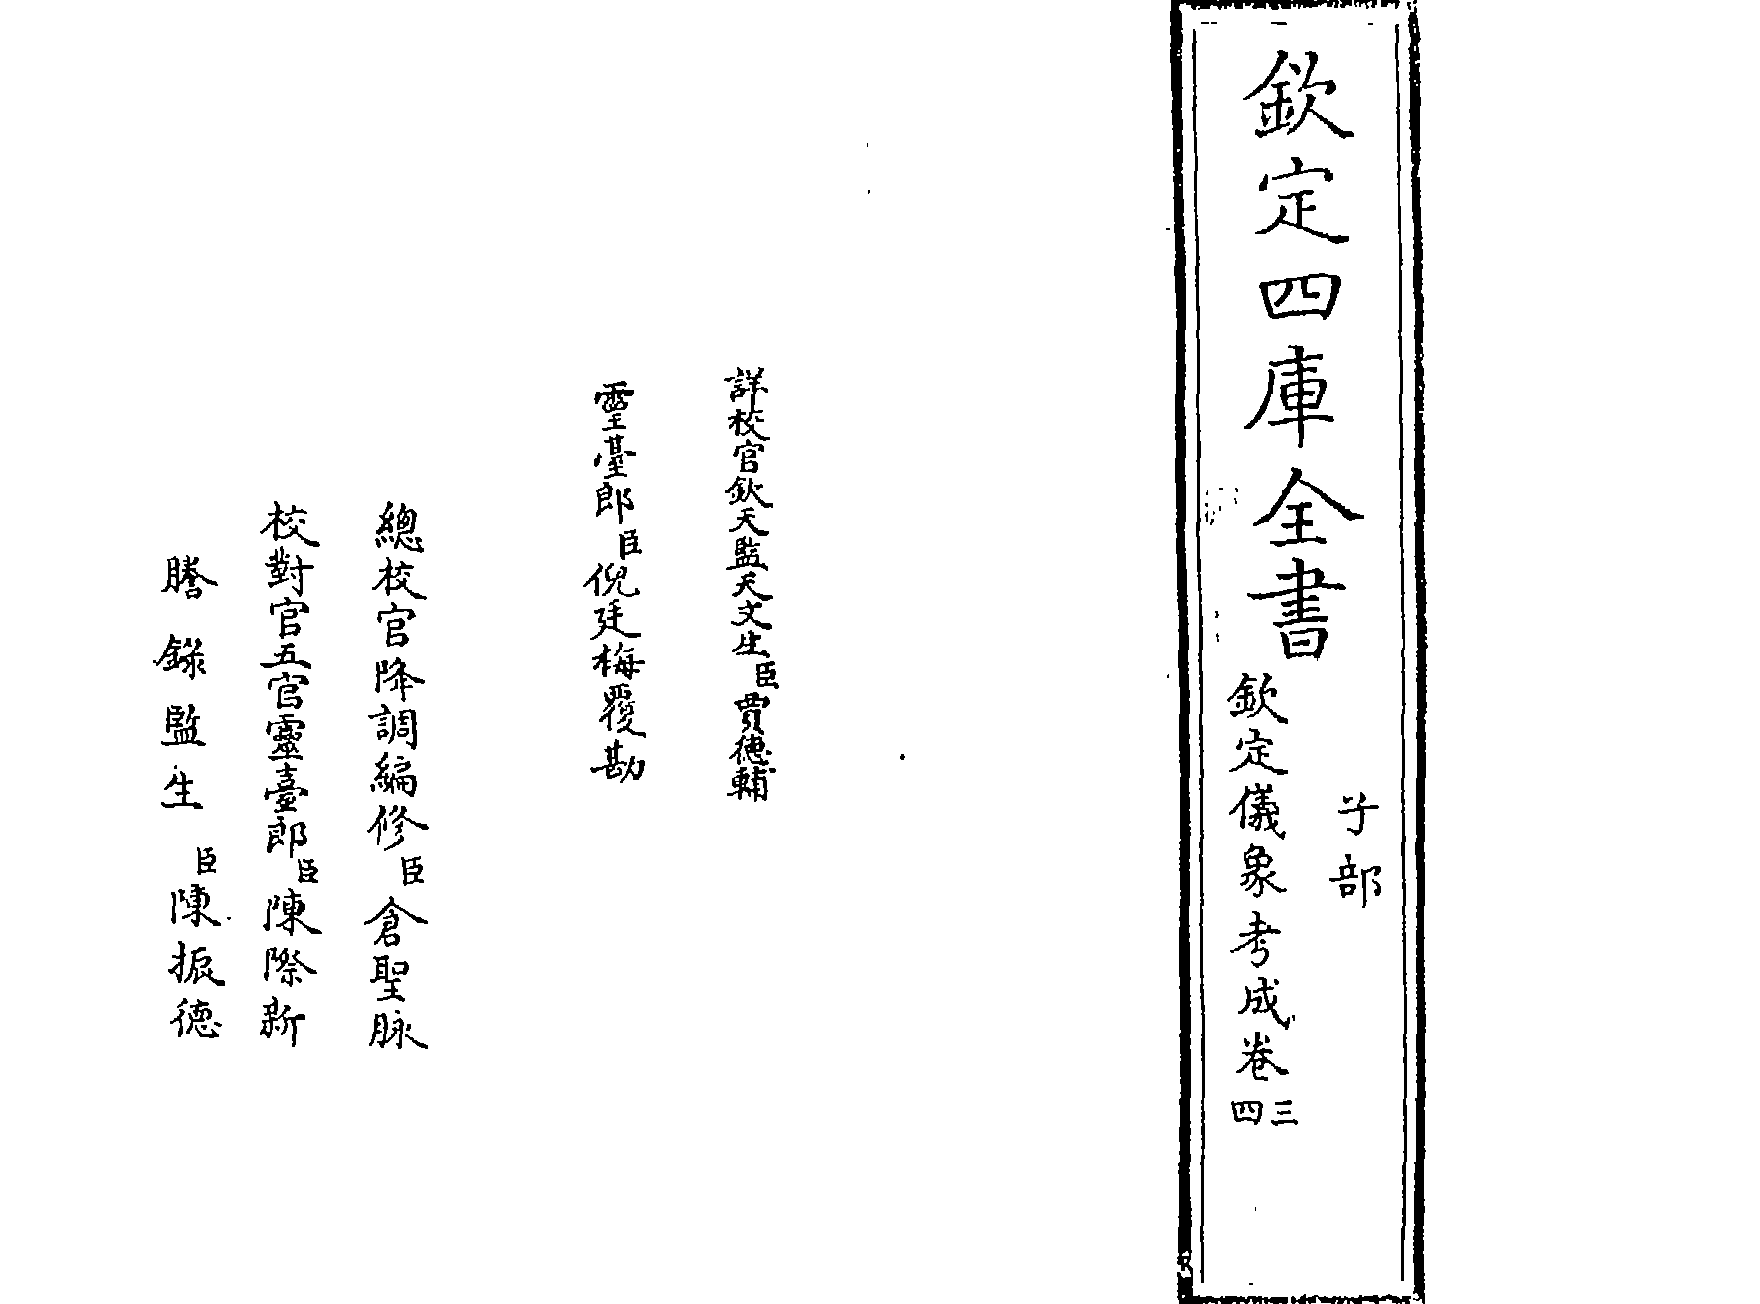
\includegraphics[width=\paperwidth,height=\paperheight,keepaspectratio]{img/0520.png}\clearpage
\begin{正文}
% ---- 册793 葉521 ----
\SetPageNumber{1}
欽定四庫全書\换行
欽定儀象考成卷三\换行
　恒星黄道經緯度表二\换行
　　黄道元枵宫\双列{\右小列{赤道度附}\左小列{}}\换行
\char"200B\relax\换行
\char"200B\relax\换行
\char"200B\relax\换行
\char"200B\relax\换行
\char"200B\relax\换行
\char"200B\relax\换行
\char"200B\relax\换行
\char"200B\relax\换行
\char"200B\relax\换行
\char"200B\relax\换行
\char"200B\relax\换行
\char"200B\relax
\par
\end{正文}\clearpage
\嵌图{142.64pt}{198.62pt}{846.47pt}{592.55pt}{img/0524.png}
\begin{正文}
% ---- 册793 葉524 图版 ----
\SetPageNumber{2}
\插图页
\char"200B\relax\换行
\char"200B\relax\换行
\char"200B\relax\换行
\char"200B\relax\换行
\char"200B\relax\换行
\char"200B\relax\换行
\char"200B\relax\换行
\char"200B\relax\换行
\char"200B\relax\换行
\char"200B\relax\换行
\char"200B\relax\换行
\char"200B\relax\换行
\char"200B\relax\换行
\char"200B\relax\换行
\char"200B\relax\换行
\char"200B\relax
\恢复丝栏\par
\end{正文}\clearpage
\嵌图{144.63pt}{197.19pt}{842.50pt}{595.40pt}{img/0525.png}
\begin{正文}
% ---- 册793 葉525 图版 ----
\SetPageNumber{3}
\插图页
\char"200B\relax\换行
\char"200B\relax\换行
\char"200B\relax\换行
\char"200B\relax\换行
\char"200B\relax\换行
\char"200B\relax\换行
\char"200B\relax\换行
\char"200B\relax\换行
\char"200B\relax\换行
\char"200B\relax\换行
\char"200B\relax\换行
\char"200B\relax\换行
\char"200B\relax\换行
\char"200B\relax\换行
\char"200B\relax\换行
\char"200B\relax
\恢复丝栏\par
\end{正文}\clearpage
\嵌图{142.68pt}{200.11pt}{846.40pt}{589.58pt}{img/0528.png}
\begin{正文}
% ---- 册793 葉528 图版 ----
\SetPageNumber{4}
\插图页
\char"200B\relax\换行
\char"200B\relax\换行
\char"200B\relax\换行
\char"200B\relax\换行
\char"200B\relax\换行
\char"200B\relax\换行
\char"200B\relax\换行
\char"200B\relax\换行
\char"200B\relax\换行
\char"200B\relax\换行
\char"200B\relax\换行
\char"200B\relax\换行
\char"200B\relax\换行
\char"200B\relax\换行
\char"200B\relax\换行
\char"200B\relax
\恢复丝栏\par
\end{正文}\clearpage
\嵌图{144.68pt}{202.93pt}{842.41pt}{583.94pt}{img/0529.png}
\begin{正文}
% ---- 册793 葉529 图版 ----
\SetPageNumber{5}
\插图页
\char"200B\relax\换行
\char"200B\relax\换行
\char"200B\relax\换行
\char"200B\relax\换行
\char"200B\relax\换行
\char"200B\relax\换行
\char"200B\relax\换行
\char"200B\relax\换行
\char"200B\relax\换行
\char"200B\relax\换行
\char"200B\relax\换行
\char"200B\relax\换行
\char"200B\relax\换行
\char"200B\relax\换行
\char"200B\relax\换行
\char"200B\relax
\恢复丝栏\par
\end{正文}\clearpage
\嵌图{144.63pt}{202.38pt}{842.50pt}{585.03pt}{img/0532.png}
\begin{正文}
% ---- 册793 葉532 图版 ----
\SetPageNumber{6}
\插图页
\char"200B\relax\换行
\char"200B\relax\换行
\char"200B\relax\换行
\char"200B\relax\换行
\char"200B\relax\换行
\char"200B\relax\换行
\char"200B\relax\换行
\char"200B\relax\换行
\char"200B\relax\换行
\char"200B\relax\换行
\char"200B\relax\换行
\char"200B\relax\换行
\char"200B\relax\换行
\char"200B\relax\换行
\char"200B\relax\换行
\char"200B\relax
\恢复丝栏\par
\end{正文}\clearpage
\嵌图{144.63pt}{201.44pt}{842.50pt}{586.92pt}{img/0533.png}
\begin{正文}
% ---- 册793 葉533 图版 ----
\SetPageNumber{7}
\插图页
\char"200B\relax\换行
\char"200B\relax\换行
\char"200B\relax\换行
\char"200B\relax\换行
\char"200B\relax\换行
\char"200B\relax\换行
\char"200B\relax\换行
\char"200B\relax\换行
\char"200B\relax\换行
\char"200B\relax\换行
\char"200B\relax\换行
\char"200B\relax\换行
\char"200B\relax\换行
\char"200B\relax\换行
\char"200B\relax\换行
\char"200B\relax
\恢复丝栏\par
\end{正文}\clearpage
\嵌图{142.68pt}{199.14pt}{846.40pt}{591.50pt}{img/0536.png}
\begin{正文}
% ---- 册793 葉536 图版 ----
\SetPageNumber{8}
\插图页
\char"200B\relax\换行
\char"200B\relax\换行
\char"200B\relax\换行
\char"200B\relax\换行
\char"200B\relax\换行
\char"200B\relax\换行
\char"200B\relax\换行
\char"200B\relax\换行
\char"200B\relax\换行
\char"200B\relax\换行
\char"200B\relax\换行
\char"200B\relax\换行
\char"200B\relax\换行
\char"200B\relax\换行
\char"200B\relax\换行
\char"200B\relax
\恢复丝栏\par
\end{正文}\clearpage
\嵌图{148.67pt}{201.53pt}{834.42pt}{586.72pt}{img/0537.png}
\begin{正文}
% ---- 册793 葉537 图版 ----
\SetPageNumber{9}
\插图页
\char"200B\relax\换行
\char"200B\relax\换行
\char"200B\relax\换行
\char"200B\relax\换行
\char"200B\relax\换行
\char"200B\relax\换行
\char"200B\relax\换行
\char"200B\relax\换行
\char"200B\relax\换行
\char"200B\relax\换行
\char"200B\relax\换行
\char"200B\relax\换行
\char"200B\relax\换行
\char"200B\relax\换行
\char"200B\relax\换行
\char"200B\relax
\恢复丝栏\par
\end{正文}\clearpage
\嵌图{144.68pt}{202.35pt}{842.41pt}{585.08pt}{img/0540.png}
\begin{正文}
% ---- 册793 葉540 图版 ----
\SetPageNumber{10}
\插图页
\char"200B\relax\换行
\char"200B\relax\换行
\char"200B\relax\换行
\char"200B\relax\换行
\char"200B\relax\换行
\char"200B\relax\换行
\char"200B\relax\换行
\char"200B\relax\换行
\char"200B\relax\换行
\char"200B\relax\换行
\char"200B\relax\换行
\char"200B\relax\换行
\char"200B\relax\换行
\char"200B\relax\换行
\char"200B\relax\换行
\char"200B\relax
\恢复丝栏\par
\end{正文}\clearpage
\嵌图{144.68pt}{201.91pt}{842.41pt}{585.98pt}{img/0541.png}
\begin{正文}
% ---- 册793 葉541 图版 ----
\SetPageNumber{11}
\插图页
\char"200B\relax\换行
\char"200B\relax\换行
\char"200B\relax\换行
\char"200B\relax\换行
\char"200B\relax\换行
\char"200B\relax\换行
\char"200B\relax\换行
\char"200B\relax\换行
\char"200B\relax\换行
\char"200B\relax\换行
\char"200B\relax\换行
\char"200B\relax\换行
\char"200B\relax\换行
\char"200B\relax\换行
\char"200B\relax\换行
\char"200B\relax
\恢复丝栏\par
\end{正文}\clearpage
\嵌图{144.63pt}{200.50pt}{842.50pt}{588.79pt}{img/0544.png}
\begin{正文}
% ---- 册793 葉544 图版 ----
\SetPageNumber{12}
\插图页
\char"200B\relax\换行
\char"200B\relax\换行
\char"200B\relax\换行
\char"200B\relax\换行
\char"200B\relax\换行
\char"200B\relax\换行
\char"200B\relax\换行
\char"200B\relax\换行
\char"200B\relax\换行
\char"200B\relax\换行
\char"200B\relax\换行
\char"200B\relax\换行
\char"200B\relax\换行
\char"200B\relax\换行
\char"200B\relax\换行
\char"200B\relax
\恢复丝栏\par
\end{正文}\clearpage
\嵌图{142.64pt}{199.58pt}{846.47pt}{590.64pt}{img/0545.png}
\begin{正文}
% ---- 册793 葉545 图版 ----
\SetPageNumber{13}
\插图页
\char"200B\relax\换行
\char"200B\relax\换行
\char"200B\relax\换行
\char"200B\relax\换行
\char"200B\relax\换行
\char"200B\relax\换行
\char"200B\relax\换行
\char"200B\relax\换行
\char"200B\relax\换行
\char"200B\relax\换行
\char"200B\relax\换行
\char"200B\relax\换行
\char"200B\relax\换行
\char"200B\relax\换行
\char"200B\relax\换行
\char"200B\relax
\恢复丝栏\par
\end{正文}\clearpage
\嵌图{144.72pt}{206.16pt}{842.31pt}{577.47pt}{img/0548.png}
\begin{正文}
% ---- 册793 葉548 图版 ----
\SetPageNumber{14}
\插图页
\char"200B\relax\换行
\char"200B\relax\换行
\char"200B\relax\换行
\char"200B\relax\换行
\char"200B\relax\换行
\char"200B\relax\换行
\char"200B\relax\换行
\char"200B\relax\换行
\char"200B\relax\换行
\char"200B\relax\换行
\char"200B\relax\换行
\char"200B\relax\换行
\char"200B\relax\换行
\char"200B\relax\换行
\char"200B\relax\换行
\char"200B\relax
\恢复丝栏\par
\end{正文}\clearpage
\嵌图{144.72pt}{200.52pt}{842.31pt}{588.75pt}{img/0549.png}
\begin{正文}
% ---- 册793 葉549 图版 ----
\SetPageNumber{15}
\插图页
\char"200B\relax\换行
\char"200B\relax\换行
\char"200B\relax\换行
\char"200B\relax\换行
\char"200B\relax\换行
\char"200B\relax\换行
\char"200B\relax\换行
\char"200B\relax\换行
\char"200B\relax\换行
\char"200B\relax\换行
\char"200B\relax\换行
\char"200B\relax\换行
\char"200B\relax\换行
\char"200B\relax\换行
\char"200B\relax\换行
\char"200B\relax
\恢复丝栏\par
\end{正文}\clearpage
\嵌图{144.59pt}{200.99pt}{842.59pt}{587.82pt}{img/0552.png}
\begin{正文}
% ---- 册793 葉552 图版 ----
\SetPageNumber{16}
\插图页
\char"200B\relax\换行
\char"200B\relax\换行
\char"200B\relax\换行
\char"200B\relax\换行
\char"200B\relax\换行
\char"200B\relax\换行
\char"200B\relax\换行
\char"200B\relax\换行
\char"200B\relax\换行
\char"200B\relax\换行
\char"200B\relax\换行
\char"200B\relax\换行
\char"200B\relax\换行
\char"200B\relax\换行
\char"200B\relax\换行
\char"200B\relax
\恢复丝栏\par
\end{正文}\clearpage
\嵌图{146.56pt}{200.06pt}{838.64pt}{589.68pt}{img/0553.png}
\begin{正文}
% ---- 册793 葉553 图版 ----
\SetPageNumber{17}
\插图页
\char"200B\relax\换行
\char"200B\relax\换行
\char"200B\relax\换行
\char"200B\relax\换行
\char"200B\relax\换行
\char"200B\relax\换行
\char"200B\relax\换行
\char"200B\relax\换行
\char"200B\relax\换行
\char"200B\relax\换行
\char"200B\relax\换行
\char"200B\relax\换行
\char"200B\relax\换行
\char"200B\relax\换行
\char"200B\relax\换行
\char"200B\relax
\恢复丝栏\par
\end{正文}\clearpage
\嵌图{144.59pt}{200.52pt}{842.59pt}{588.75pt}{img/0556.png}
\begin{正文}
% ---- 册793 葉556 图版 ----
\SetPageNumber{18}
\插图页
\char"200B\relax\换行
\char"200B\relax\换行
\char"200B\relax\换行
\char"200B\relax\换行
\char"200B\relax\换行
\char"200B\relax\换行
\char"200B\relax\换行
\char"200B\relax\换行
\char"200B\relax\换行
\char"200B\relax\换行
\char"200B\relax\换行
\char"200B\relax\换行
\char"200B\relax\换行
\char"200B\relax\换行
\char"200B\relax\换行
\char"200B\relax
\恢复丝栏\par
\end{正文}\clearpage
\嵌图{151.71pt}{213.17pt}{828.34pt}{563.44pt}{img/0557.png}
\begin{正文}
% ---- 册793 葉557 图版 ----
\SetPageNumber{19}
\插图页
\char"200B\relax\换行
\char"200B\relax\换行
\char"200B\relax\换行
\char"200B\relax\换行
\char"200B\relax\换行
\char"200B\relax\换行
\char"200B\relax\换行
\char"200B\relax\换行
\char"200B\relax\换行
\char"200B\relax\换行
\char"200B\relax\换行
\char"200B\relax\换行
\char"200B\relax\换行
\char"200B\relax\换行
\char"200B\relax\换行
\char"200B\relax
\恢复丝栏\par
\end{正文}\clearpage
\嵌图{144.68pt}{202.00pt}{842.41pt}{585.78pt}{img/0560.png}
\begin{正文}
% ---- 册793 葉560 图版 ----
\SetPageNumber{20}
\插图页
\char"200B\relax\换行
\char"200B\relax\换行
\char"200B\relax\换行
\char"200B\relax\换行
\char"200B\relax\换行
\char"200B\relax\换行
\char"200B\relax\换行
\char"200B\relax\换行
\char"200B\relax\换行
\char"200B\relax\换行
\char"200B\relax\换行
\char"200B\relax\换行
\char"200B\relax\换行
\char"200B\relax\换行
\char"200B\relax\换行
\char"200B\relax
\恢复丝栏\par
\end{正文}\clearpage
\嵌图{146.67pt}{201.52pt}{838.42pt}{586.75pt}{img/0561.png}
\begin{正文}
% ---- 册793 葉561 图版 ----
\SetPageNumber{21}
\插图页
\char"200B\relax\换行
\char"200B\relax\换行
\char"200B\relax\换行
\char"200B\relax\换行
\char"200B\relax\换行
\char"200B\relax\换行
\char"200B\relax\换行
\char"200B\relax\换行
\char"200B\relax\换行
\char"200B\relax\换行
\char"200B\relax\换行
\char"200B\relax\换行
\char"200B\relax\换行
\char"200B\relax\换行
\char"200B\relax\换行
\char"200B\relax
\恢复丝栏\par
\end{正文}\clearpage
\嵌图{146.62pt}{201.47pt}{838.53pt}{586.86pt}{img/0564.png}
\begin{正文}
% ---- 册793 葉564 图版 ----
\SetPageNumber{22}
\插图页
\char"200B\relax\换行
\char"200B\relax\换行
\char"200B\relax\换行
\char"200B\relax\换行
\char"200B\relax\换行
\char"200B\relax\换行
\char"200B\relax\换行
\char"200B\relax\换行
\char"200B\relax\换行
\char"200B\relax\换行
\char"200B\relax\换行
\char"200B\relax\换行
\char"200B\relax\换行
\char"200B\relax\换行
\char"200B\relax\换行
\char"200B\relax
\恢复丝栏\par
\end{正文}\clearpage
\嵌图{179.21pt}{217.75pt}{659.61pt}{575.08pt}{img/0565.png}
\begin{正文}
% ---- 册793 葉565 ----
\SetPageNumber{23}
\插图页
\char"200B\relax\换行
\char"200B\relax\换行
\char"200B\relax\换行
\char"200B\relax\换行
\char"200B\relax\换行
\char"200B\relax\换行
\char"200B\relax\换行
\char"200B\relax\换行
\恢复丝栏
\char"200B\relax\换行
\char"200B\relax\换行
\char"200B\relax\换行
\char"200B\relax\换行
\char"200B\relax\换行
\char"200B\relax\换行
\char"200B\relax\换行
欽定儀象考成卷三
\par

% ======== 卷四（8行21字）========
\par\end{正文}\clearpage
\chapter*{欽定儀象考成卷四}
\begin{正文}
% ---- 册793 葉568 ----
\SetPageNumber{1}
欽定四庫全書\换行
欽定儀象考成卷四\换行
　恒星黄道經緯度表三\换行
　　黄道娵訾宫\双列{\右小列{赤道度附}\左小列{}}\换行
\char"200B\relax\换行
\char"200B\relax\换行
\char"200B\relax\换行
\char"200B\relax\换行
\char"200B\relax\换行
\char"200B\relax\换行
\char"200B\relax\换行
\char"200B\relax\换行
\char"200B\relax\换行
\char"200B\relax\换行
\char"200B\relax\换行
\char"200B\relax
\par
\end{正文}\clearpage
\嵌图{144.68pt}{201.04pt}{842.41pt}{587.70pt}{img/0569.png}
\begin{正文}
% ---- 册793 葉569 图版 ----
\SetPageNumber{2}
\插图页
\char"200B\relax\换行
\char"200B\relax\换行
\char"200B\relax\换行
\char"200B\relax\换行
\char"200B\relax\换行
\char"200B\relax\换行
\char"200B\relax\换行
\char"200B\relax\换行
\char"200B\relax\换行
\char"200B\relax\换行
\char"200B\relax\换行
\char"200B\relax\换行
\char"200B\relax\换行
\char"200B\relax\换行
\char"200B\relax\换行
\char"200B\relax
\恢复丝栏\par
\end{正文}\clearpage
\嵌图{146.62pt}{199.63pt}{838.53pt}{590.54pt}{img/0572.png}
\begin{正文}
% ---- 册793 葉572 图版 ----
\SetPageNumber{3}
\插图页
\char"200B\relax\换行
\char"200B\relax\换行
\char"200B\relax\换行
\char"200B\relax\换行
\char"200B\relax\换行
\char"200B\relax\换行
\char"200B\relax\换行
\char"200B\relax\换行
\char"200B\relax\换行
\char"200B\relax\换行
\char"200B\relax\换行
\char"200B\relax\换行
\char"200B\relax\换行
\char"200B\relax\换行
\char"200B\relax\换行
\char"200B\relax
\恢复丝栏\par
\end{正文}\clearpage
\嵌图{142.64pt}{197.20pt}{846.47pt}{595.40pt}{img/0573.png}
\begin{正文}
% ---- 册793 葉573 图版 ----
\SetPageNumber{4}
\插图页
\char"200B\relax\换行
\char"200B\relax\换行
\char"200B\relax\换行
\char"200B\relax\换行
\char"200B\relax\换行
\char"200B\relax\换行
\char"200B\relax\换行
\char"200B\relax\换行
\char"200B\relax\换行
\char"200B\relax\换行
\char"200B\relax\换行
\char"200B\relax\换行
\char"200B\relax\换行
\char"200B\relax\换行
\char"200B\relax\换行
\char"200B\relax
\恢复丝栏\par
\end{正文}\clearpage
\嵌图{148.61pt}{201.04pt}{834.55pt}{587.70pt}{img/0576.png}
\begin{正文}
% ---- 册793 葉576 图版 ----
\SetPageNumber{5}
\插图页
\char"200B\relax\换行
\char"200B\relax\换行
\char"200B\relax\换行
\char"200B\relax\换行
\char"200B\relax\换行
\char"200B\relax\换行
\char"200B\relax\换行
\char"200B\relax\换行
\char"200B\relax\换行
\char"200B\relax\换行
\char"200B\relax\换行
\char"200B\relax\换行
\char"200B\relax\换行
\char"200B\relax\换行
\char"200B\relax\换行
\char"200B\relax
\恢复丝栏\par
\end{正文}\clearpage
\嵌图{146.62pt}{201.02pt}{838.53pt}{587.74pt}{img/0577.png}
\begin{正文}
% ---- 册793 葉577 图版 ----
\SetPageNumber{6}
\插图页
\char"200B\relax\换行
\char"200B\relax\换行
\char"200B\relax\换行
\char"200B\relax\换行
\char"200B\relax\换行
\char"200B\relax\换行
\char"200B\relax\换行
\char"200B\relax\换行
\char"200B\relax\换行
\char"200B\relax\换行
\char"200B\relax\换行
\char"200B\relax\换行
\char"200B\relax\换行
\char"200B\relax\换行
\char"200B\relax\换行
\char"200B\relax
\恢复丝栏\par
\end{正文}\clearpage
\嵌图{148.61pt}{200.56pt}{834.55pt}{588.68pt}{img/0580.png}
\begin{正文}
% ---- 册793 葉580 图版 ----
\SetPageNumber{7}
\插图页
\char"200B\relax\换行
\char"200B\relax\换行
\char"200B\relax\换行
\char"200B\relax\换行
\char"200B\relax\换行
\char"200B\relax\换行
\char"200B\relax\换行
\char"200B\relax\换行
\char"200B\relax\换行
\char"200B\relax\换行
\char"200B\relax\换行
\char"200B\relax\换行
\char"200B\relax\换行
\char"200B\relax\换行
\char"200B\relax\换行
\char"200B\relax
\恢复丝栏\par
\end{正文}\clearpage
\嵌图{148.61pt}{202.87pt}{834.55pt}{584.06pt}{img/0581.png}
\begin{正文}
% ---- 册793 葉581 图版 ----
\SetPageNumber{8}
\插图页
\char"200B\relax\换行
\char"200B\relax\换行
\char"200B\relax\换行
\char"200B\relax\换行
\char"200B\relax\换行
\char"200B\relax\换行
\char"200B\relax\换行
\char"200B\relax\换行
\char"200B\relax\换行
\char"200B\relax\换行
\char"200B\relax\换行
\char"200B\relax\换行
\char"200B\relax\换行
\char"200B\relax\换行
\char"200B\relax\换行
\char"200B\relax
\恢复丝栏\par
\end{正文}\clearpage
\嵌图{140.66pt}{206.21pt}{850.45pt}{577.36pt}{img/0584.png}
\begin{正文}
% ---- 册793 葉584 图版 ----
\SetPageNumber{9}
\插图页
\char"200B\relax\换行
\char"200B\relax\换行
\char"200B\relax\换行
\char"200B\relax\换行
\char"200B\relax\换行
\char"200B\relax\换行
\char"200B\relax\换行
\char"200B\relax\换行
\char"200B\relax\换行
\char"200B\relax\换行
\char"200B\relax\换行
\char"200B\relax\换行
\char"200B\relax\换行
\char"200B\relax\换行
\char"200B\relax\换行
\char"200B\relax
\恢复丝栏\par
\end{正文}\clearpage
\嵌图{144.63pt}{201.93pt}{842.50pt}{585.93pt}{img/0585.png}
\begin{正文}
% ---- 册793 葉585 图版 ----
\SetPageNumber{10}
\插图页
\char"200B\relax\换行
\char"200B\relax\换行
\char"200B\relax\换行
\char"200B\relax\换行
\char"200B\relax\换行
\char"200B\relax\换行
\char"200B\relax\换行
\char"200B\relax\换行
\char"200B\relax\换行
\char"200B\relax\换行
\char"200B\relax\换行
\char"200B\relax\换行
\char"200B\relax\换行
\char"200B\relax\换行
\char"200B\relax\换行
\char"200B\relax
\恢复丝栏\par
\end{正文}\clearpage
\嵌图{146.56pt}{199.95pt}{838.64pt}{589.90pt}{img/0588.png}
\begin{正文}
% ---- 册793 葉588 图版 ----
\SetPageNumber{11}
\插图页
\char"200B\relax\换行
\char"200B\relax\换行
\char"200B\relax\换行
\char"200B\relax\换行
\char"200B\relax\换行
\char"200B\relax\换行
\char"200B\relax\换行
\char"200B\relax\换行
\char"200B\relax\换行
\char"200B\relax\换行
\char"200B\relax\换行
\char"200B\relax\换行
\char"200B\relax\换行
\char"200B\relax\换行
\char"200B\relax\换行
\char"200B\relax
\恢复丝栏\par
\end{正文}\clearpage
\嵌图{146.56pt}{200.43pt}{838.64pt}{588.92pt}{img/0589.png}
\begin{正文}
% ---- 册793 葉589 图版 ----
\SetPageNumber{12}
\插图页
\char"200B\relax\换行
\char"200B\relax\换行
\char"200B\relax\换行
\char"200B\relax\换行
\char"200B\relax\换行
\char"200B\relax\换行
\char"200B\relax\换行
\char"200B\relax\换行
\char"200B\relax\换行
\char"200B\relax\换行
\char"200B\relax\换行
\char"200B\relax\换行
\char"200B\relax\换行
\char"200B\relax\换行
\char"200B\relax\换行
\char"200B\relax
\恢复丝栏\par
\end{正文}\clearpage
\嵌图{146.67pt}{204.26pt}{838.42pt}{581.26pt}{img/0592.png}
\begin{正文}
% ---- 册793 葉592 图版 ----
\SetPageNumber{13}
\插图页
\char"200B\relax\换行
\char"200B\relax\换行
\char"200B\relax\换行
\char"200B\relax\换行
\char"200B\relax\换行
\char"200B\relax\换行
\char"200B\relax\换行
\char"200B\relax\换行
\char"200B\relax\换行
\char"200B\relax\换行
\char"200B\relax\换行
\char"200B\relax\换行
\char"200B\relax\换行
\char"200B\relax\换行
\char"200B\relax\换行
\char"200B\relax
\恢复丝栏\par
\end{正文}\clearpage
\嵌图{146.67pt}{201.92pt}{838.42pt}{585.96pt}{img/0593.png}
\begin{正文}
% ---- 册793 葉593 图版 ----
\SetPageNumber{14}
\插图页
\char"200B\relax\换行
\char"200B\relax\换行
\char"200B\relax\换行
\char"200B\relax\换行
\char"200B\relax\换行
\char"200B\relax\换行
\char"200B\relax\换行
\char"200B\relax\换行
\char"200B\relax\换行
\char"200B\relax\换行
\char"200B\relax\换行
\char"200B\relax\换行
\char"200B\relax\换行
\char"200B\relax\换行
\char"200B\relax\换行
\char"200B\relax
\恢复丝栏\par
\end{正文}\clearpage
\嵌图{146.62pt}{203.26pt}{838.53pt}{583.27pt}{img/0596.png}
\begin{正文}
% ---- 册793 葉596 图版 ----
\SetPageNumber{15}
\插图页
\char"200B\relax\换行
\char"200B\relax\换行
\char"200B\relax\换行
\char"200B\relax\换行
\char"200B\relax\换行
\char"200B\relax\换行
\char"200B\relax\换行
\char"200B\relax\换行
\char"200B\relax\换行
\char"200B\relax\换行
\char"200B\relax\换行
\char"200B\relax\换行
\char"200B\relax\换行
\char"200B\relax\换行
\char"200B\relax\换行
\char"200B\relax
\恢复丝栏\par
\end{正文}\clearpage
\嵌图{144.63pt}{199.97pt}{842.50pt}{589.85pt}{img/0597.png}
\begin{正文}
% ---- 册793 葉597 图版 ----
\SetPageNumber{16}
\插图页
\char"200B\relax\换行
\char"200B\relax\换行
\char"200B\relax\换行
\char"200B\relax\换行
\char"200B\relax\换行
\char"200B\relax\换行
\char"200B\relax\换行
\char"200B\relax\换行
\char"200B\relax\换行
\char"200B\relax\换行
\char"200B\relax\换行
\char"200B\relax\换行
\char"200B\relax\换行
\char"200B\relax\换行
\char"200B\relax\换行
\char"200B\relax
\恢复丝栏\par
\end{正文}\clearpage
\嵌图{146.56pt}{202.76pt}{838.64pt}{584.26pt}{img/0600.png}
\begin{正文}
% ---- 册793 葉600 图版 ----
\SetPageNumber{17}
\插图页
\char"200B\relax\换行
\char"200B\relax\换行
\char"200B\relax\换行
\char"200B\relax\换行
\char"200B\relax\换行
\char"200B\relax\换行
\char"200B\relax\换行
\char"200B\relax\换行
\char"200B\relax\换行
\char"200B\relax\换行
\char"200B\relax\换行
\char"200B\relax\换行
\char"200B\relax\换行
\char"200B\relax\换行
\char"200B\relax\换行
\char"200B\relax
\恢复丝栏\par
\end{正文}\clearpage
\嵌图{148.54pt}{201.39pt}{834.68pt}{587.01pt}{img/0601.png}
\begin{正文}
% ---- 册793 葉601 图版 ----
\SetPageNumber{18}
\插图页
\char"200B\relax\换行
\char"200B\relax\换行
\char"200B\relax\换行
\char"200B\relax\换行
\char"200B\relax\换行
\char"200B\relax\换行
\char"200B\relax\换行
\char"200B\relax\换行
\char"200B\relax\换行
\char"200B\relax\换行
\char"200B\relax\换行
\char"200B\relax\换行
\char"200B\relax\换行
\char"200B\relax\换行
\char"200B\relax\换行
\char"200B\relax
\恢复丝栏\par
\end{正文}\clearpage
\嵌图{155.09pt}{218.94pt}{392.93pt}{573.89pt}{img/0604.png}
\begin{正文}
% ---- 册793 葉604 ----
\SetPageNumber{19}
\插图页
\char"200B\relax\换行
\char"200B\relax\换行
\char"200B\relax\换行
\char"200B\relax\换行
\char"200B\relax\换行
\char"200B\relax\换行
\char"200B\relax\换行
\char"200B\relax\换行
\恢复丝栏
\char"200B\relax\换行
\char"200B\relax\换行
\char"200B\relax\换行
\char"200B\relax\换行
\char"200B\relax\换行
\char"200B\relax\换行
\char"200B\relax\换行
欽定儀象考成卷四
\par

\par\end{正文}\clearpage

  % ======== 卷五（8行21字）========
\chapter*{欽定儀象考成卷五}
\begin{正文}
\end{正文}\clearpage
\thispagestyle{empty}\noindent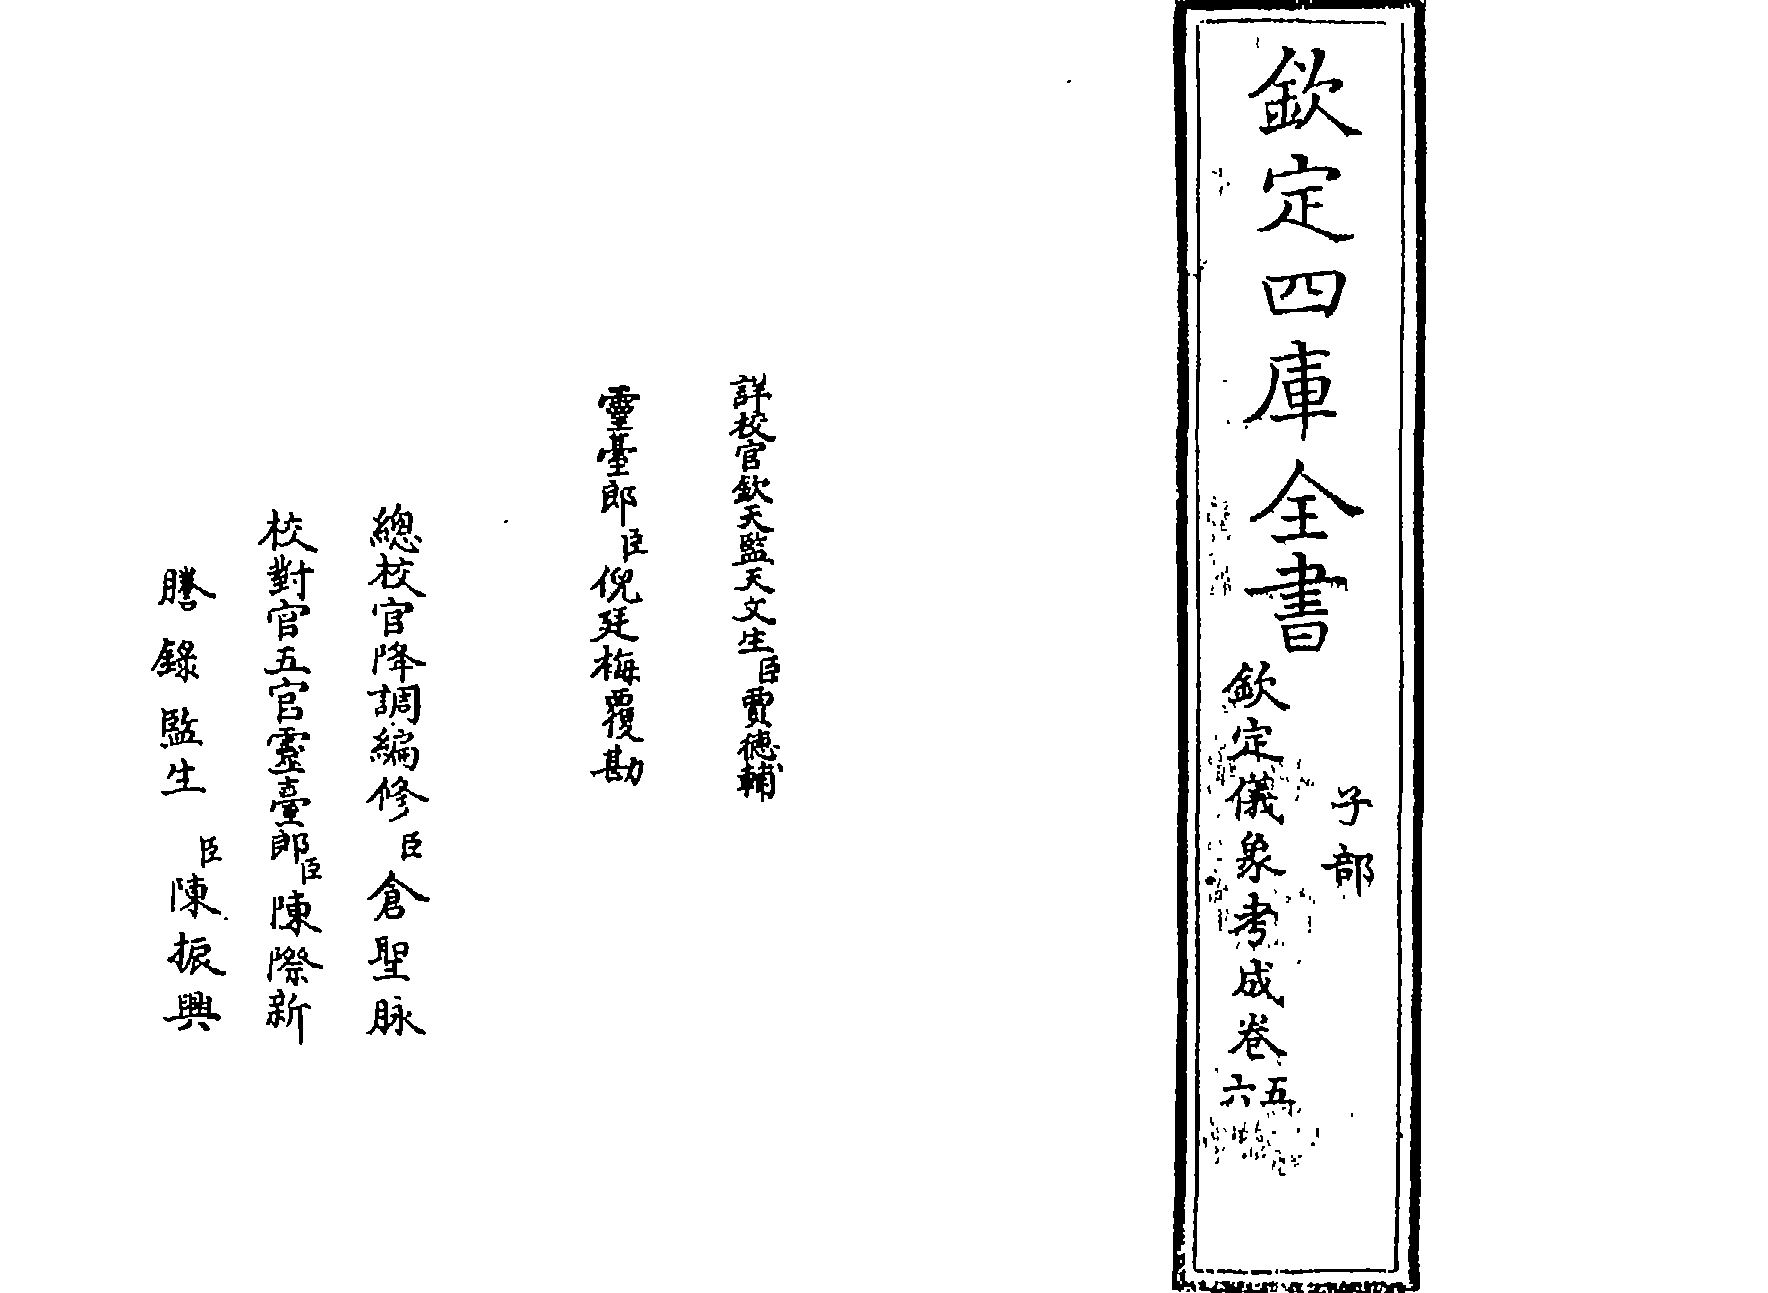
\includegraphics[width=\paperwidth,height=\paperheight,keepaspectratio]{img/0608.png}\clearpage
\begin{正文}
% ---- 册793 葉609 ----
\SetPageNumber{1}
欽定四庫全書\换行
欽定儀象考成卷五\换行
　恒星黄道經緯度表四\换行
　　黄道降婁宫\换行
\char"200B\relax\换行
\char"200B\relax\换行
\char"200B\relax\换行
\char"200B\relax\换行
\char"200B\relax\换行
\char"200B\relax\换行
\char"200B\relax\换行
\char"200B\relax\换行
\char"200B\relax\换行
\char"200B\relax\换行
\char"200B\relax\换行
\char"200B\relax
\par
\end{正文}\clearpage
\嵌图{144.63pt}{201.03pt}{842.50pt}{587.73pt}{img/0612.png}
\begin{正文}
% ---- 册793 葉612 图版 ----
\SetPageNumber{2}
\插图页
\char"200B\relax\换行
\char"200B\relax\换行
\char"200B\relax\换行
\char"200B\relax\换行
\char"200B\relax\换行
\char"200B\relax\换行
\char"200B\relax\换行
\char"200B\relax\换行
\char"200B\relax\换行
\char"200B\relax\换行
\char"200B\relax\换行
\char"200B\relax\换行
\char"200B\relax\换行
\char"200B\relax\换行
\char"200B\relax\换行
\char"200B\relax
\恢复丝栏\par
\end{正文}\clearpage
\嵌图{142.64pt}{201.47pt}{846.47pt}{586.84pt}{img/0613.png}
\begin{正文}
% ---- 册793 葉613 图版 ----
\SetPageNumber{3}
\插图页
\char"200B\relax\换行
\char"200B\relax\换行
\char"200B\relax\换行
\char"200B\relax\换行
\char"200B\relax\换行
\char"200B\relax\换行
\char"200B\relax\换行
\char"200B\relax\换行
\char"200B\relax\换行
\char"200B\relax\换行
\char"200B\relax\换行
\char"200B\relax\换行
\char"200B\relax\换行
\char"200B\relax\换行
\char"200B\relax\换行
\char"200B\relax
\恢复丝栏\par
\end{正文}\clearpage
\嵌图{144.59pt}{201.04pt}{842.59pt}{587.72pt}{img/0616.png}
\begin{正文}
% ---- 册793 葉616 图版 ----
\SetPageNumber{4}
\插图页
\char"200B\relax\换行
\char"200B\relax\换行
\char"200B\relax\换行
\char"200B\relax\换行
\char"200B\relax\换行
\char"200B\relax\换行
\char"200B\relax\换行
\char"200B\relax\换行
\char"200B\relax\换行
\char"200B\relax\换行
\char"200B\relax\换行
\char"200B\relax\换行
\char"200B\relax\换行
\char"200B\relax\换行
\char"200B\relax\换行
\char"200B\relax
\恢复丝栏\par
\end{正文}\clearpage
\嵌图{148.54pt}{201.51pt}{834.68pt}{586.77pt}{img/0617.png}
\begin{正文}
% ---- 册793 葉617 图版 ----
\SetPageNumber{5}
\插图页
\char"200B\relax\换行
\char"200B\relax\换行
\char"200B\relax\换行
\char"200B\relax\换行
\char"200B\relax\换行
\char"200B\relax\换行
\char"200B\relax\换行
\char"200B\relax\换行
\char"200B\relax\换行
\char"200B\relax\换行
\char"200B\relax\换行
\char"200B\relax\换行
\char"200B\relax\换行
\char"200B\relax\换行
\char"200B\relax\换行
\char"200B\relax
\恢复丝栏\par
\end{正文}\clearpage
\嵌图{144.63pt}{201.46pt}{842.50pt}{586.87pt}{img/0620.png}
\begin{正文}
% ---- 册793 葉620 图版 ----
\SetPageNumber{6}
\插图页
\char"200B\relax\换行
\char"200B\relax\换行
\char"200B\relax\换行
\char"200B\relax\换行
\char"200B\relax\换行
\char"200B\relax\换行
\char"200B\relax\换行
\char"200B\relax\换行
\char"200B\relax\换行
\char"200B\relax\换行
\char"200B\relax\换行
\char"200B\relax\换行
\char"200B\relax\换行
\char"200B\relax\换行
\char"200B\relax\换行
\char"200B\relax
\恢复丝栏\par
\end{正文}\clearpage
\嵌图{144.63pt}{201.88pt}{842.50pt}{586.04pt}{img/0621.png}
\begin{正文}
% ---- 册793 葉621 图版 ----
\SetPageNumber{7}
\插图页
\char"200B\relax\换行
\char"200B\relax\换行
\char"200B\relax\换行
\char"200B\relax\换行
\char"200B\relax\换行
\char"200B\relax\换行
\char"200B\relax\换行
\char"200B\relax\换行
\char"200B\relax\换行
\char"200B\relax\换行
\char"200B\relax\换行
\char"200B\relax\换行
\char"200B\relax\换行
\char"200B\relax\换行
\char"200B\relax\换行
\char"200B\relax
\恢复丝栏\par
\end{正文}\clearpage
\嵌图{144.63pt}{202.91pt}{842.50pt}{583.97pt}{img/0624.png}
\begin{正文}
% ---- 册793 葉624 图版 ----
\SetPageNumber{8}
\插图页
\char"200B\relax\换行
\char"200B\relax\换行
\char"200B\relax\换行
\char"200B\relax\换行
\char"200B\relax\换行
\char"200B\relax\换行
\char"200B\relax\换行
\char"200B\relax\换行
\char"200B\relax\换行
\char"200B\relax\换行
\char"200B\relax\换行
\char"200B\relax\换行
\char"200B\relax\换行
\char"200B\relax\换行
\char"200B\relax\换行
\char"200B\relax
\恢复丝栏\par
\end{正文}\clearpage
\嵌图{146.62pt}{203.36pt}{838.53pt}{583.08pt}{img/0625.png}
\begin{正文}
% ---- 册793 葉625 图版 ----
\SetPageNumber{9}
\插图页
\char"200B\relax\换行
\char"200B\relax\换行
\char"200B\relax\换行
\char"200B\relax\换行
\char"200B\relax\换行
\char"200B\relax\换行
\char"200B\relax\换行
\char"200B\relax\换行
\char"200B\relax\换行
\char"200B\relax\换行
\char"200B\relax\换行
\char"200B\relax\换行
\char"200B\relax\换行
\char"200B\relax\换行
\char"200B\relax\换行
\char"200B\relax
\恢复丝栏\par
\end{正文}\clearpage
\嵌图{148.54pt}{201.88pt}{834.68pt}{586.02pt}{img/0628.png}
\begin{正文}
% ---- 册793 葉628 图版 ----
\SetPageNumber{10}
\插图页
\char"200B\relax\换行
\char"200B\relax\换行
\char"200B\relax\换行
\char"200B\relax\换行
\char"200B\relax\换行
\char"200B\relax\换行
\char"200B\relax\换行
\char"200B\relax\换行
\char"200B\relax\换行
\char"200B\relax\换行
\char"200B\relax\换行
\char"200B\relax\换行
\char"200B\relax\换行
\char"200B\relax\换行
\char"200B\relax\换行
\char"200B\relax
\恢复丝栏\par
\end{正文}\clearpage
\嵌图{146.56pt}{200.93pt}{838.64pt}{587.93pt}{img/0629.png}
\begin{正文}
% ---- 册793 葉629 图版 ----
\SetPageNumber{11}
\插图页
\char"200B\relax\换行
\char"200B\relax\换行
\char"200B\relax\换行
\char"200B\relax\换行
\char"200B\relax\换行
\char"200B\relax\换行
\char"200B\relax\换行
\char"200B\relax\换行
\char"200B\relax\换行
\char"200B\relax\换行
\char"200B\relax\换行
\char"200B\relax\换行
\char"200B\relax\换行
\char"200B\relax\换行
\char"200B\relax\换行
\char"200B\relax
\恢复丝栏\par
\end{正文}\clearpage
\嵌图{142.64pt}{201.95pt}{846.47pt}{585.90pt}{img/0632.png}
\begin{正文}
% ---- 册793 葉632 图版 ----
\SetPageNumber{12}
\插图页
\char"200B\relax\换行
\char"200B\relax\换行
\char"200B\relax\换行
\char"200B\relax\换行
\char"200B\relax\换行
\char"200B\relax\换行
\char"200B\relax\换行
\char"200B\relax\换行
\char"200B\relax\换行
\char"200B\relax\换行
\char"200B\relax\换行
\char"200B\relax\换行
\char"200B\relax\换行
\char"200B\relax\换行
\char"200B\relax\换行
\char"200B\relax
\恢复丝栏\par
\end{正文}\clearpage
\嵌图{144.63pt}{200.54pt}{842.50pt}{588.72pt}{img/0633.png}
\begin{正文}
% ---- 册793 葉633 图版 ----
\SetPageNumber{13}
\插图页
\char"200B\relax\换行
\char"200B\relax\换行
\char"200B\relax\换行
\char"200B\relax\换行
\char"200B\relax\换行
\char"200B\relax\换行
\char"200B\relax\换行
\char"200B\relax\换行
\char"200B\relax\换行
\char"200B\relax\换行
\char"200B\relax\换行
\char"200B\relax\换行
\char"200B\relax\换行
\char"200B\relax\换行
\char"200B\relax\换行
\char"200B\relax
\恢复丝栏\par
\end{正文}\clearpage
\嵌图{144.63pt}{200.93pt}{842.50pt}{587.93pt}{img/0636.png}
\begin{正文}
% ---- 册793 葉636 图版 ----
\SetPageNumber{14}
\插图页
\char"200B\relax\换行
\char"200B\relax\换行
\char"200B\relax\换行
\char"200B\relax\换行
\char"200B\relax\换行
\char"200B\relax\换行
\char"200B\relax\换行
\char"200B\relax\换行
\char"200B\relax\换行
\char"200B\relax\换行
\char"200B\relax\换行
\char"200B\relax\换行
\char"200B\relax\换行
\char"200B\relax\换行
\char"200B\relax\换行
\char"200B\relax
\恢复丝栏\par
\end{正文}\clearpage
\嵌图{148.61pt}{199.50pt}{834.55pt}{590.78pt}{img/0637.png}
\begin{正文}
% ---- 册793 葉637 图版 ----
\SetPageNumber{15}
\插图页
\char"200B\relax\换行
\char"200B\relax\换行
\char"200B\relax\换行
\char"200B\relax\换行
\char"200B\relax\换行
\char"200B\relax\换行
\char"200B\relax\换行
\char"200B\relax\换行
\char"200B\relax\换行
\char"200B\relax\换行
\char"200B\relax\换行
\char"200B\relax\换行
\char"200B\relax\换行
\char"200B\relax\换行
\char"200B\relax\换行
\char"200B\relax
\恢复丝栏\par
\end{正文}\clearpage
\嵌图{144.63pt}{201.95pt}{842.50pt}{585.90pt}{img/0640.png}
\begin{正文}
% ---- 册793 葉640 图版 ----
\SetPageNumber{16}
\插图页
\char"200B\relax\换行
\char"200B\relax\换行
\char"200B\relax\换行
\char"200B\relax\换行
\char"200B\relax\换行
\char"200B\relax\换行
\char"200B\relax\换行
\char"200B\relax\换行
\char"200B\relax\换行
\char"200B\relax\换行
\char"200B\relax\换行
\char"200B\relax\换行
\char"200B\relax\换行
\char"200B\relax\换行
\char"200B\relax\换行
\char"200B\relax
\恢复丝栏\par
\end{正文}\clearpage
\嵌图{144.63pt}{201.02pt}{842.50pt}{587.76pt}{img/0641.png}
\begin{正文}
% ---- 册793 葉641 图版 ----
\SetPageNumber{17}
\插图页
\char"200B\relax\换行
\char"200B\relax\换行
\char"200B\relax\换行
\char"200B\relax\换行
\char"200B\relax\换行
\char"200B\relax\换行
\char"200B\relax\换行
\char"200B\relax\换行
\char"200B\relax\换行
\char"200B\relax\换行
\char"200B\relax\换行
\char"200B\relax\换行
\char"200B\relax\换行
\char"200B\relax\换行
\char"200B\relax\换行
\char"200B\relax
\恢复丝栏\par
\end{正文}\clearpage
\嵌图{146.67pt}{200.52pt}{838.42pt}{588.75pt}{img/0644.png}
\begin{正文}
% ---- 册793 葉644 图版 ----
\SetPageNumber{18}
\插图页
\char"200B\relax\换行
\char"200B\relax\换行
\char"200B\relax\换行
\char"200B\relax\换行
\char"200B\relax\换行
\char"200B\relax\换行
\char"200B\relax\换行
\char"200B\relax\换行
\char"200B\relax\换行
\char"200B\relax\换行
\char"200B\relax\换行
\char"200B\relax\换行
\char"200B\relax\换行
\char"200B\relax\换行
\char"200B\relax\换行
\char"200B\relax
\恢复丝栏\par
\end{正文}\clearpage
\嵌图{150.67pt}{200.99pt}{830.43pt}{587.80pt}{img/0645.png}
\begin{正文}
% ---- 册793 葉645 图版 ----
\SetPageNumber{19}
\插图页
\char"200B\relax\换行
\char"200B\relax\换行
\char"200B\relax\换行
\char"200B\relax\换行
\char"200B\relax\换行
\char"200B\relax\换行
\char"200B\relax\换行
\char"200B\relax\换行
\char"200B\relax\换行
\char"200B\relax\换行
\char"200B\relax\换行
\char"200B\relax\换行
\char"200B\relax\换行
\char"200B\relax\换行
\char"200B\relax\换行
\char"200B\relax
\恢复丝栏\par
\end{正文}\clearpage
\嵌图{140.63pt}{199.98pt}{850.50pt}{589.83pt}{img/0648.png}
\begin{正文}
% ---- 册793 葉648 图版 ----
\SetPageNumber{20}
\插图页
\char"200B\relax\换行
\char"200B\relax\换行
\char"200B\relax\换行
\char"200B\relax\换行
\char"200B\relax\换行
\char"200B\relax\换行
\char"200B\relax\换行
\char"200B\relax\换行
\char"200B\relax\换行
\char"200B\relax\换行
\char"200B\relax\换行
\char"200B\relax\换行
\char"200B\relax\换行
\char"200B\relax\换行
\char"200B\relax\换行
\char"200B\relax
\恢复丝栏\par
\end{正文}\clearpage
\嵌图{146.56pt}{200.49pt}{838.64pt}{588.82pt}{img/0649.png}
\begin{正文}
% ---- 册793 葉649 图版 ----
\SetPageNumber{21}
\插图页
\char"200B\relax\换行
\char"200B\relax\换行
\char"200B\relax\换行
\char"200B\relax\换行
\char"200B\relax\换行
\char"200B\relax\换行
\char"200B\relax\换行
\char"200B\relax\换行
\char"200B\relax\换行
\char"200B\relax\换行
\char"200B\relax\换行
\char"200B\relax\换行
\char"200B\relax\换行
\char"200B\relax\换行
\char"200B\relax\换行
\char"200B\relax
\恢复丝栏\par
\end{正文}\clearpage
\嵌图{126.91pt}{215.07pt}{762.93pt}{577.76pt}{img/0652.png}
\begin{正文}
% ---- 册793 葉652 ----
\SetPageNumber{22}
\插图页
\char"200B\relax\换行
\char"200B\relax\换行
\char"200B\relax\换行
\char"200B\relax\换行
\char"200B\relax\换行
\char"200B\relax\换行
\char"200B\relax\换行
\char"200B\relax\换行
\恢复丝栏
\char"200B\relax\换行
\char"200B\relax\换行
\char"200B\relax\换行
\char"200B\relax\换行
\char"200B\relax\换行
\char"200B\relax\换行
欽定儀象考成卷五\换行
\char"200B\relax
\par

% ======== 卷六（8行21字）========
\par\end{正文}\clearpage
\chapter*{欽定儀象考成卷六}
\begin{正文}
% ---- 册793 葉653 ----
\SetPageNumber{1}
欽定四庫全書\换行
欽定儀象考成卷六\换行
　恒星黄道經緯度表五\换行
　　黄道大梁宫\双列{\右小列{赤道度附}\左小列{}}\换行
\char"200B\relax\换行
\char"200B\relax\换行
\char"200B\relax\换行
\char"200B\relax\换行
\char"200B\relax\换行
\char"200B\relax\换行
\char"200B\relax\换行
\char"200B\relax\换行
\char"200B\relax\换行
\char"200B\relax\换行
\char"200B\relax\换行
\char"200B\relax
\par
\end{正文}\clearpage
\嵌图{142.68pt}{198.67pt}{846.40pt}{592.45pt}{img/0656.png}
\begin{正文}
% ---- 册793 葉656 图版 ----
\SetPageNumber{2}
\插图页
\char"200B\relax\换行
\char"200B\relax\换行
\char"200B\relax\换行
\char"200B\relax\换行
\char"200B\relax\换行
\char"200B\relax\换行
\char"200B\relax\换行
\char"200B\relax\换行
\char"200B\relax\换行
\char"200B\relax\换行
\char"200B\relax\换行
\char"200B\relax\换行
\char"200B\relax\换行
\char"200B\relax\换行
\char"200B\relax\换行
\char"200B\relax
\恢复丝栏\par
\end{正文}\clearpage
\嵌图{146.67pt}{203.90pt}{838.42pt}{582.00pt}{img/0657.png}
\begin{正文}
% ---- 册793 葉657 图版 ----
\SetPageNumber{3}
\插图页
\char"200B\relax\换行
\char"200B\relax\换行
\char"200B\relax\换行
\char"200B\relax\换行
\char"200B\relax\换行
\char"200B\relax\换行
\char"200B\relax\换行
\char"200B\relax\换行
\char"200B\relax\换行
\char"200B\relax\换行
\char"200B\relax\换行
\char"200B\relax\换行
\char"200B\relax\换行
\char"200B\relax\换行
\char"200B\relax\换行
\char"200B\relax
\恢复丝栏\par
\end{正文}\clearpage
\嵌图{148.61pt}{201.92pt}{834.55pt}{585.94pt}{img/0660.png}
\begin{正文}
% ---- 册793 葉660 图版 ----
\SetPageNumber{4}
\插图页
\char"200B\relax\换行
\char"200B\relax\换行
\char"200B\relax\换行
\char"200B\relax\换行
\char"200B\relax\换行
\char"200B\relax\换行
\char"200B\relax\换行
\char"200B\relax\换行
\char"200B\relax\换行
\char"200B\relax\换行
\char"200B\relax\换行
\char"200B\relax\换行
\char"200B\relax\换行
\char"200B\relax\换行
\char"200B\relax\换行
\char"200B\relax
\恢复丝栏\par
\end{正文}\clearpage
\嵌图{146.62pt}{201.41pt}{838.53pt}{586.96pt}{img/0661.png}
\begin{正文}
% ---- 册793 葉661 图版 ----
\SetPageNumber{5}
\插图页
\char"200B\relax\换行
\char"200B\relax\换行
\char"200B\relax\换行
\char"200B\relax\换行
\char"200B\relax\换行
\char"200B\relax\换行
\char"200B\relax\换行
\char"200B\relax\换行
\char"200B\relax\换行
\char"200B\relax\换行
\char"200B\relax\换行
\char"200B\relax\换行
\char"200B\relax\换行
\char"200B\relax\换行
\char"200B\relax\换行
\char"200B\relax
\恢复丝栏\par
\end{正文}\clearpage
\嵌图{146.67pt}{201.55pt}{838.42pt}{586.69pt}{img/0664.png}
\begin{正文}
% ---- 册793 葉664 图版 ----
\SetPageNumber{6}
\插图页
\char"200B\relax\换行
\char"200B\relax\换行
\char"200B\relax\换行
\char"200B\relax\换行
\char"200B\relax\换行
\char"200B\relax\换行
\char"200B\relax\换行
\char"200B\relax\换行
\char"200B\relax\换行
\char"200B\relax\换行
\char"200B\relax\换行
\char"200B\relax\换行
\char"200B\relax\换行
\char"200B\relax\换行
\char"200B\relax\换行
\char"200B\relax
\恢复丝栏\par
\end{正文}\clearpage
\嵌图{144.68pt}{200.53pt}{842.41pt}{588.73pt}{img/0665.png}
\begin{正文}
% ---- 册793 葉665 图版 ----
\SetPageNumber{7}
\插图页
\char"200B\relax\换行
\char"200B\relax\换行
\char"200B\relax\换行
\char"200B\relax\换行
\char"200B\relax\换行
\char"200B\relax\换行
\char"200B\relax\换行
\char"200B\relax\换行
\char"200B\relax\换行
\char"200B\relax\换行
\char"200B\relax\换行
\char"200B\relax\换行
\char"200B\relax\换行
\char"200B\relax\换行
\char"200B\relax\换行
\char"200B\relax
\恢复丝栏\par
\end{正文}\clearpage
\嵌图{146.67pt}{200.50pt}{838.42pt}{588.79pt}{img/0668.png}
\begin{正文}
% ---- 册793 葉668 图版 ----
\SetPageNumber{8}
\插图页
\char"200B\relax\换行
\char"200B\relax\换行
\char"200B\relax\换行
\char"200B\relax\换行
\char"200B\relax\换行
\char"200B\relax\换行
\char"200B\relax\换行
\char"200B\relax\换行
\char"200B\relax\换行
\char"200B\relax\换行
\char"200B\relax\换行
\char"200B\relax\换行
\char"200B\relax\换行
\char"200B\relax\换行
\char"200B\relax\换行
\char"200B\relax
\恢复丝栏\par
\end{正文}\clearpage
\嵌图{148.67pt}{199.52pt}{834.42pt}{590.75pt}{img/0669.png}
\begin{正文}
% ---- 册793 葉669 图版 ----
\SetPageNumber{9}
\插图页
\char"200B\relax\换行
\char"200B\relax\换行
\char"200B\relax\换行
\char"200B\relax\换行
\char"200B\relax\换行
\char"200B\relax\换行
\char"200B\relax\换行
\char"200B\relax\换行
\char"200B\relax\换行
\char"200B\relax\换行
\char"200B\relax\换行
\char"200B\relax\换行
\char"200B\relax\换行
\char"200B\relax\换行
\char"200B\relax\换行
\char"200B\relax
\恢复丝栏\par
\end{正文}\clearpage
\嵌图{144.63pt}{201.94pt}{842.50pt}{585.91pt}{img/0672.png}
\begin{正文}
% ---- 册793 葉672 图版 ----
\SetPageNumber{10}
\插图页
\char"200B\relax\换行
\char"200B\relax\换行
\char"200B\relax\换行
\char"200B\relax\换行
\char"200B\relax\换行
\char"200B\relax\换行
\char"200B\relax\换行
\char"200B\relax\换行
\char"200B\relax\换行
\char"200B\relax\换行
\char"200B\relax\换行
\char"200B\relax\换行
\char"200B\relax\换行
\char"200B\relax\换行
\char"200B\relax\换行
\char"200B\relax
\恢复丝栏\par
\end{正文}\clearpage
\嵌图{144.63pt}{202.90pt}{842.50pt}{583.99pt}{img/0673.png}
\begin{正文}
% ---- 册793 葉673 图版 ----
\SetPageNumber{11}
\插图页
\char"200B\relax\换行
\char"200B\relax\换行
\char"200B\relax\换行
\char"200B\relax\换行
\char"200B\relax\换行
\char"200B\relax\换行
\char"200B\relax\换行
\char"200B\relax\换行
\char"200B\relax\换行
\char"200B\relax\换行
\char"200B\relax\换行
\char"200B\relax\换行
\char"200B\relax\换行
\char"200B\relax\换行
\char"200B\relax\换行
\char"200B\relax
\恢复丝栏\par
\end{正文}\clearpage
\嵌图{148.73pt}{201.95pt}{834.29pt}{585.88pt}{img/0676.png}
\begin{正文}
% ---- 册793 葉676 图版 ----
\SetPageNumber{12}
\插图页
\char"200B\relax\换行
\char"200B\relax\换行
\char"200B\relax\换行
\char"200B\relax\换行
\char"200B\relax\换行
\char"200B\relax\换行
\char"200B\relax\换行
\char"200B\relax\换行
\char"200B\relax\换行
\char"200B\relax\换行
\char"200B\relax\换行
\char"200B\relax\换行
\char"200B\relax\换行
\char"200B\relax\换行
\char"200B\relax\换行
\char"200B\relax
\恢复丝栏\par
\end{正文}\clearpage
\嵌图{146.73pt}{198.17pt}{838.30pt}{593.45pt}{img/0677.png}
\begin{正文}
% ---- 册793 葉677 图版 ----
\SetPageNumber{13}
\插图页
\char"200B\relax\换行
\char"200B\relax\换行
\char"200B\relax\换行
\char"200B\relax\换行
\char"200B\relax\换行
\char"200B\relax\换行
\char"200B\relax\换行
\char"200B\relax\换行
\char"200B\relax\换行
\char"200B\relax\换行
\char"200B\relax\换行
\char"200B\relax\换行
\char"200B\relax\换行
\char"200B\relax\换行
\char"200B\relax\换行
\char"200B\relax
\恢复丝栏\par
\end{正文}\clearpage
\嵌图{146.56pt}{202.90pt}{838.64pt}{583.99pt}{img/0680.png}
\begin{正文}
% ---- 册793 葉680 图版 ----
\SetPageNumber{14}
\插图页
\char"200B\relax\换行
\char"200B\relax\换行
\char"200B\relax\换行
\char"200B\relax\换行
\char"200B\relax\换行
\char"200B\relax\换行
\char"200B\relax\换行
\char"200B\relax\换行
\char"200B\relax\换行
\char"200B\relax\换行
\char"200B\relax\换行
\char"200B\relax\换行
\char"200B\relax\换行
\char"200B\relax\换行
\char"200B\relax\换行
\char"200B\relax
\恢复丝栏\par
\end{正文}\clearpage
\嵌图{148.54pt}{205.26pt}{834.68pt}{579.28pt}{img/0681.png}
\begin{正文}
% ---- 册793 葉681 图版 ----
\SetPageNumber{15}
\插图页
\char"200B\relax\换行
\char"200B\relax\换行
\char"200B\relax\换行
\char"200B\relax\换行
\char"200B\relax\换行
\char"200B\relax\换行
\char"200B\relax\换行
\char"200B\relax\换行
\char"200B\relax\换行
\char"200B\relax\换行
\char"200B\relax\换行
\char"200B\relax\换行
\char"200B\relax\换行
\char"200B\relax\换行
\char"200B\relax\换行
\char"200B\relax
\恢复丝栏\par
\end{正文}\clearpage
\嵌图{146.56pt}{203.84pt}{838.64pt}{582.11pt}{img/0684.png}
\begin{正文}
% ---- 册793 葉684 图版 ----
\SetPageNumber{16}
\插图页
\char"200B\relax\换行
\char"200B\relax\换行
\char"200B\relax\换行
\char"200B\relax\换行
\char"200B\relax\换行
\char"200B\relax\换行
\char"200B\relax\换行
\char"200B\relax\换行
\char"200B\relax\换行
\char"200B\relax\换行
\char"200B\relax\换行
\char"200B\relax\换行
\char"200B\relax\换行
\char"200B\relax\换行
\char"200B\relax\换行
\char"200B\relax
\恢复丝栏\par
\end{正文}\clearpage
\嵌图{146.56pt}{200.49pt}{838.64pt}{588.80pt}{img/0685.png}
\begin{正文}
% ---- 册793 葉685 图版 ----
\SetPageNumber{17}
\插图页
\char"200B\relax\换行
\char"200B\relax\换行
\char"200B\relax\换行
\char"200B\relax\换行
\char"200B\relax\换行
\char"200B\relax\换行
\char"200B\relax\换行
\char"200B\relax\换行
\char"200B\relax\换行
\char"200B\relax\换行
\char"200B\relax\换行
\char"200B\relax\换行
\char"200B\relax\换行
\char"200B\relax\换行
\char"200B\relax\换行
\char"200B\relax
\恢复丝栏\par
\end{正文}\clearpage
\嵌图{140.68pt}{203.93pt}{850.39pt}{581.92pt}{img/0688.png}
\begin{正文}
% ---- 册793 葉688 图版 ----
\SetPageNumber{18}
\插图页
\char"200B\relax\换行
\char"200B\relax\换行
\char"200B\relax\换行
\char"200B\relax\换行
\char"200B\relax\换行
\char"200B\relax\换行
\char"200B\relax\换行
\char"200B\relax\换行
\char"200B\relax\换行
\char"200B\relax\换行
\char"200B\relax\换行
\char"200B\relax\换行
\char"200B\relax\换行
\char"200B\relax\换行
\char"200B\relax\换行
\char"200B\relax
\恢复丝栏\par
\end{正文}\clearpage
\嵌图{150.67pt}{200.58pt}{830.43pt}{588.62pt}{img/0689.png}
\begin{正文}
% ---- 册793 葉689 图版 ----
\SetPageNumber{19}
\插图页
\char"200B\relax\换行
\char"200B\relax\换行
\char"200B\relax\换行
\char"200B\relax\换行
\char"200B\relax\换行
\char"200B\relax\换行
\char"200B\relax\换行
\char"200B\relax\换行
\char"200B\relax\换行
\char"200B\relax\换行
\char"200B\relax\换行
\char"200B\relax\换行
\char"200B\relax\换行
\char"200B\relax\换行
\char"200B\relax\换行
\char"200B\relax
\恢复丝栏\par
\end{正文}\clearpage
\嵌图{148.61pt}{201.93pt}{834.55pt}{585.93pt}{img/0692.png}
\begin{正文}
% ---- 册793 葉692 图版 ----
\SetPageNumber{20}
\插图页
\char"200B\relax\换行
\char"200B\relax\换行
\char"200B\relax\换行
\char"200B\relax\换行
\char"200B\relax\换行
\char"200B\relax\换行
\char"200B\relax\换行
\char"200B\relax\换行
\char"200B\relax\换行
\char"200B\relax\换行
\char"200B\relax\换行
\char"200B\relax\换行
\char"200B\relax\换行
\char"200B\relax\换行
\char"200B\relax\换行
\char"200B\relax
\恢复丝栏\par
\end{正文}\clearpage
\嵌图{146.62pt}{204.25pt}{838.53pt}{581.28pt}{img/0693.png}
\begin{正文}
% ---- 册793 葉693 图版 ----
\SetPageNumber{21}
\插图页
\char"200B\relax\换行
\char"200B\relax\换行
\char"200B\relax\换行
\char"200B\relax\换行
\char"200B\relax\换行
\char"200B\relax\换行
\char"200B\relax\换行
\char"200B\relax\换行
\char"200B\relax\换行
\char"200B\relax\换行
\char"200B\relax\换行
\char"200B\relax\换行
\char"200B\relax\换行
\char"200B\relax\换行
\char"200B\relax\换行
\char"200B\relax
\恢复丝栏\par
\end{正文}\clearpage
\嵌图{144.72pt}{203.93pt}{842.31pt}{581.92pt}{img/0696.png}
\begin{正文}
% ---- 册793 葉696 图版 ----
\SetPageNumber{22}
\插图页
\char"200B\relax\换行
\char"200B\relax\换行
\char"200B\relax\换行
\char"200B\relax\换行
\char"200B\relax\换行
\char"200B\relax\换行
\char"200B\relax\换行
\char"200B\relax\换行
\char"200B\relax\换行
\char"200B\relax\换行
\char"200B\relax\换行
\char"200B\relax\换行
\char"200B\relax\换行
\char"200B\relax\换行
\char"200B\relax\换行
\char"200B\relax
\恢复丝栏\par
\end{正文}\clearpage
\嵌图{164.65pt}{222.62pt}{725.19pt}{570.21pt}{img/0697.png}
\begin{正文}
% ---- 册793 葉697 ----
\SetPageNumber{23}
\插图页
\char"200B\relax\换行
\char"200B\relax\换行
\char"200B\relax\换行
\char"200B\relax\换行
\char"200B\relax\换行
\char"200B\relax\换行
\char"200B\relax\换行
\char"200B\relax\换行
\恢复丝栏
\char"200B\relax\换行
\char"200B\relax\换行
\char"200B\relax\换行
\char"200B\relax\换行
\char"200B\relax\换行
\char"200B\relax\换行
\char"200B\relax\换行
欽定儀象考成卷六
\par

\par\end{正文}\clearpage

  \input{parts/part07}
  \thispagestyle{empty}\noindent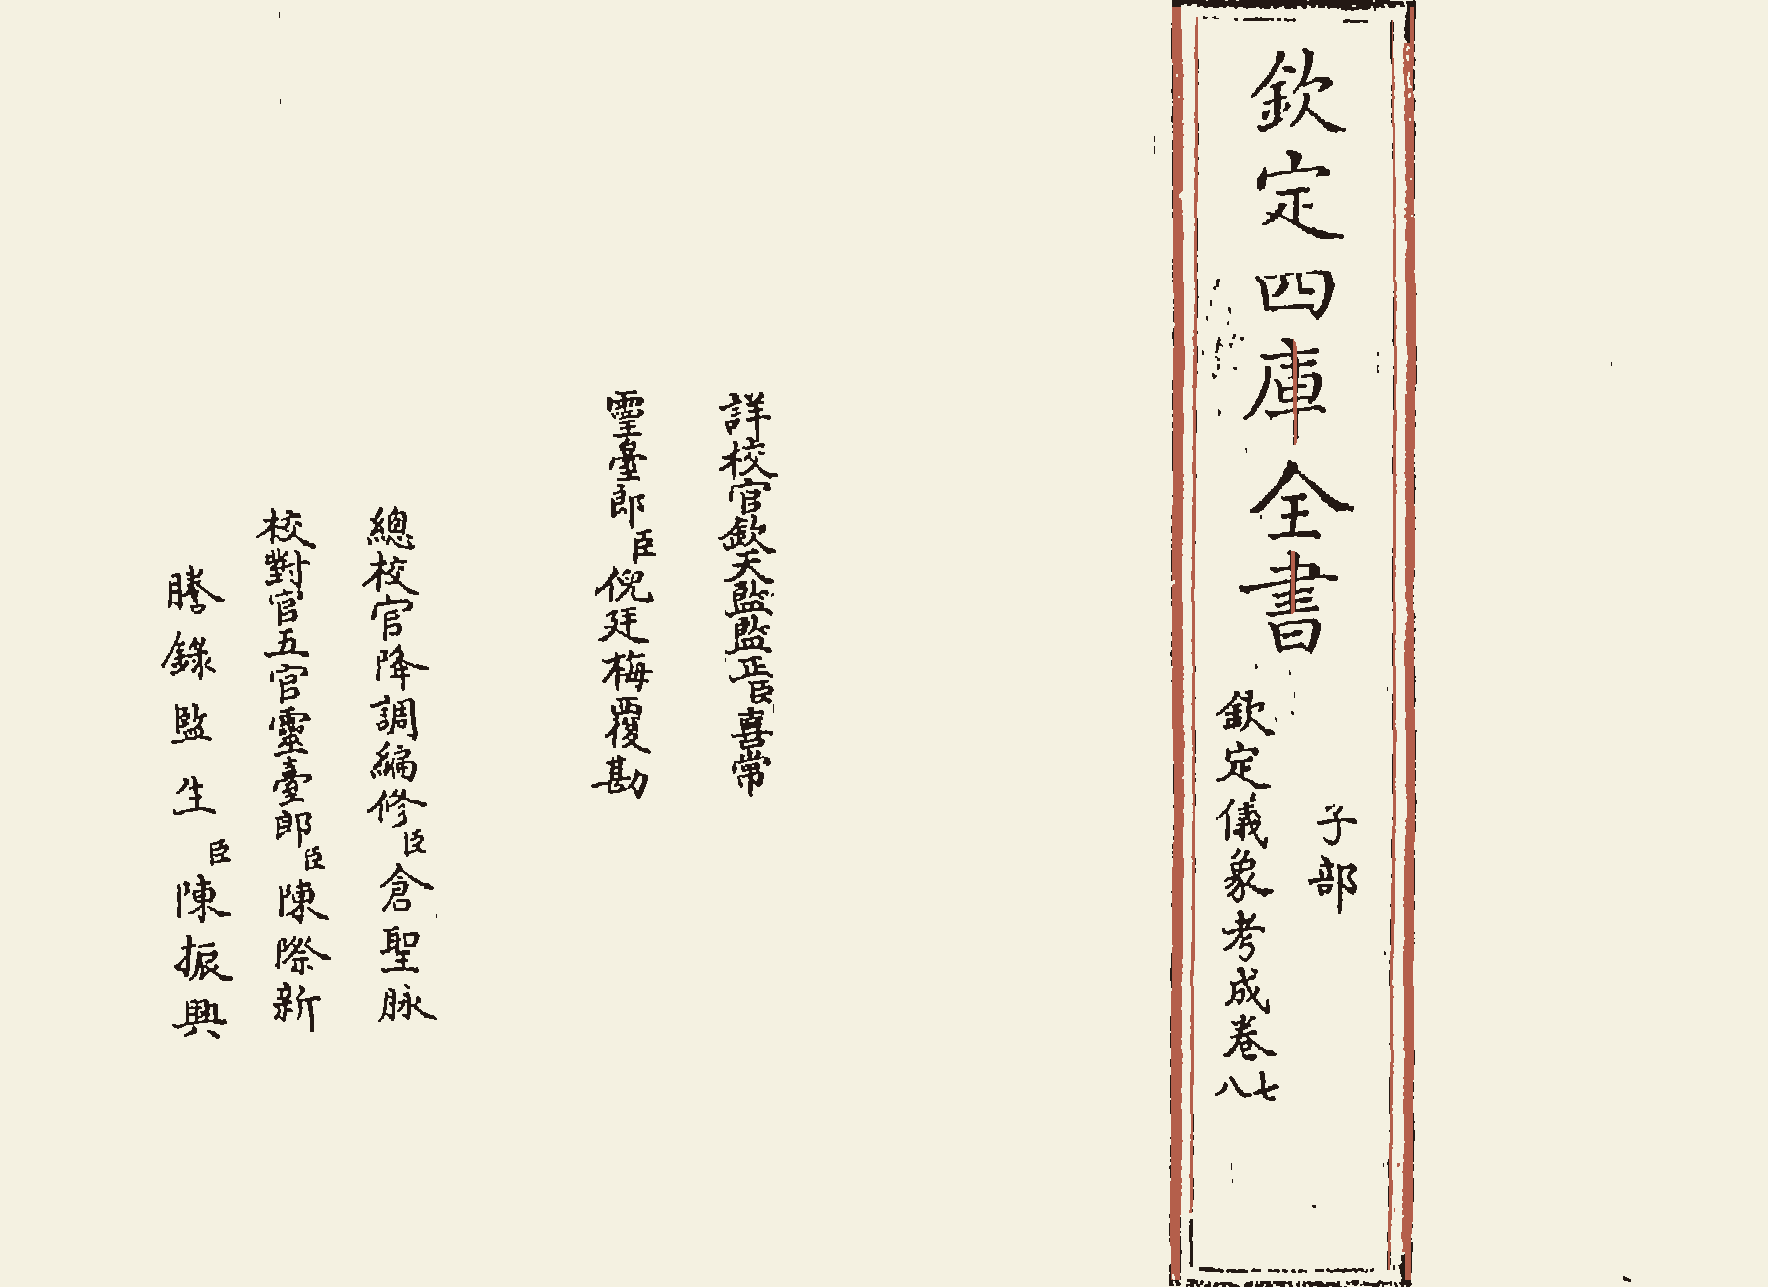
\includegraphics[width=\paperwidth,height=\paperheight,keepaspectratio]{img/0700.png}\clearpage
\begin{正文}
% ---- 册793 葉701 ----
\SetPageNumber{1}
欽定四庫全書\换行
欽定儀象考成卷七\换行
　恒星黄道經緯度表六\换行
　　黄道實沈宫\双列{\右小列{赤道度附}\左小列{}}\换行
\char"200B\relax\换行
\char"200B\relax\换行
\char"200B\relax\换行
\char"200B\relax\换行
\char"200B\relax\换行
\char"200B\relax\换行
\char"200B\relax\换行
\char"200B\relax\换行
\char"200B\relax\换行
\char"200B\relax\换行
\char"200B\relax\换行
\char"200B\relax
\par
\end{正文}\clearpage
\嵌图{146.56pt}{202.48pt}{838.64pt}{584.83pt}{img/0704.png}
\begin{正文}
% ---- 册793 葉704 图版 ----
\SetPageNumber{2}
\插图页
\char"200B\relax\换行
\char"200B\relax\换行
\char"200B\relax\换行
\char"200B\relax\换行
\char"200B\relax\换行
\char"200B\relax\换行
\char"200B\relax\换行
\char"200B\relax\换行
\char"200B\relax\换行
\char"200B\relax\换行
\char"200B\relax\换行
\char"200B\relax\换行
\char"200B\relax\换行
\char"200B\relax\换行
\char"200B\relax\换行
\char"200B\relax
\恢复丝栏\par
\end{正文}\clearpage
\嵌图{148.54pt}{201.50pt}{834.68pt}{586.80pt}{img/0705.png}
\begin{正文}
% ---- 册793 葉705 图版 ----
\SetPageNumber{3}
\插图页
\char"200B\relax\换行
\char"200B\relax\换行
\char"200B\relax\换行
\char"200B\relax\换行
\char"200B\relax\换行
\char"200B\relax\换行
\char"200B\relax\换行
\char"200B\relax\换行
\char"200B\relax\换行
\char"200B\relax\换行
\char"200B\relax\换行
\char"200B\relax\换行
\char"200B\relax\换行
\char"200B\relax\换行
\char"200B\relax\换行
\char"200B\relax
\恢复丝栏\par
\end{正文}\clearpage
\嵌图{146.62pt}{203.90pt}{838.53pt}{582.00pt}{img/0708.png}
\begin{正文}
% ---- 册793 葉708 图版 ----
\SetPageNumber{4}
\插图页
\char"200B\relax\换行
\char"200B\relax\换行
\char"200B\relax\换行
\char"200B\relax\换行
\char"200B\relax\换行
\char"200B\relax\换行
\char"200B\relax\换行
\char"200B\relax\换行
\char"200B\relax\换行
\char"200B\relax\换行
\char"200B\relax\换行
\char"200B\relax\换行
\char"200B\relax\换行
\char"200B\relax\换行
\char"200B\relax\换行
\char"200B\relax
\恢复丝栏\par
\end{正文}\clearpage
\嵌图{144.63pt}{200.99pt}{842.50pt}{587.82pt}{img/0709.png}
\begin{正文}
% ---- 册793 葉709 图版 ----
\SetPageNumber{5}
\插图页
\char"200B\relax\换行
\char"200B\relax\换行
\char"200B\relax\换行
\char"200B\relax\换行
\char"200B\relax\换行
\char"200B\relax\换行
\char"200B\relax\换行
\char"200B\relax\换行
\char"200B\relax\换行
\char"200B\relax\换行
\char"200B\relax\换行
\char"200B\relax\换行
\char"200B\relax\换行
\char"200B\relax\换行
\char"200B\relax\换行
\char"200B\relax
\恢复丝栏\par
\end{正文}\clearpage
\嵌图{140.66pt}{204.85pt}{850.45pt}{580.10pt}{img/0712.png}
\begin{正文}
% ---- 册793 葉712 图版 ----
\SetPageNumber{6}
\插图页
\char"200B\relax\换行
\char"200B\relax\换行
\char"200B\relax\换行
\char"200B\relax\换行
\char"200B\relax\换行
\char"200B\relax\换行
\char"200B\relax\换行
\char"200B\relax\换行
\char"200B\relax\换行
\char"200B\relax\换行
\char"200B\relax\换行
\char"200B\relax\换行
\char"200B\relax\换行
\char"200B\relax\换行
\char"200B\relax\换行
\char"200B\relax
\恢复丝栏\par
\end{正文}\clearpage
\嵌图{142.64pt}{204.81pt}{846.47pt}{580.16pt}{img/0713.png}
\begin{正文}
% ---- 册793 葉713 图版 ----
\SetPageNumber{7}
\插图页
\char"200B\relax\换行
\char"200B\relax\换行
\char"200B\relax\换行
\char"200B\relax\换行
\char"200B\relax\换行
\char"200B\relax\换行
\char"200B\relax\换行
\char"200B\relax\换行
\char"200B\relax\换行
\char"200B\relax\换行
\char"200B\relax\换行
\char"200B\relax\换行
\char"200B\relax\换行
\char"200B\relax\换行
\char"200B\relax\换行
\char"200B\relax
\恢复丝栏\par
\end{正文}\clearpage
\嵌图{148.54pt}{198.60pt}{834.68pt}{592.58pt}{img/0716.png}
\begin{正文}
% ---- 册793 葉716 图版 ----
\SetPageNumber{8}
\插图页
\char"200B\relax\换行
\char"200B\relax\换行
\char"200B\relax\换行
\char"200B\relax\换行
\char"200B\relax\换行
\char"200B\relax\换行
\char"200B\relax\换行
\char"200B\relax\换行
\char"200B\relax\换行
\char"200B\relax\换行
\char"200B\relax\换行
\char"200B\relax\换行
\char"200B\relax\换行
\char"200B\relax\换行
\char"200B\relax\换行
\char"200B\relax
\恢复丝栏\par
\end{正文}\clearpage
\嵌图{150.52pt}{200.46pt}{830.72pt}{588.87pt}{img/0717.png}
\begin{正文}
% ---- 册793 葉717 图版 ----
\SetPageNumber{9}
\插图页
\char"200B\relax\换行
\char"200B\relax\换行
\char"200B\relax\换行
\char"200B\relax\换行
\char"200B\relax\换行
\char"200B\relax\换行
\char"200B\relax\换行
\char"200B\relax\换行
\char"200B\relax\换行
\char"200B\relax\换行
\char"200B\relax\换行
\char"200B\relax\换行
\char"200B\relax\换行
\char"200B\relax\换行
\char"200B\relax\换行
\char"200B\relax
\恢复丝栏\par
\end{正文}\clearpage
\嵌图{142.64pt}{200.54pt}{846.47pt}{588.72pt}{img/0720.png}
\begin{正文}
% ---- 册793 葉720 图版 ----
\SetPageNumber{10}
\插图页
\char"200B\relax\换行
\char"200B\relax\换行
\char"200B\relax\换行
\char"200B\relax\换行
\char"200B\relax\换行
\char"200B\relax\换行
\char"200B\relax\换行
\char"200B\relax\换行
\char"200B\relax\换行
\char"200B\relax\换行
\char"200B\relax\换行
\char"200B\relax\换行
\char"200B\relax\换行
\char"200B\relax\换行
\char"200B\relax\换行
\char"200B\relax
\恢复丝栏\par
\end{正文}\clearpage
\嵌图{150.59pt}{203.37pt}{830.58pt}{583.06pt}{img/0721.png}
\begin{正文}
% ---- 册793 葉721 图版 ----
\SetPageNumber{11}
\插图页
\char"200B\relax\换行
\char"200B\relax\换行
\char"200B\relax\换行
\char"200B\relax\换行
\char"200B\relax\换行
\char"200B\relax\换行
\char"200B\relax\换行
\char"200B\relax\换行
\char"200B\relax\换行
\char"200B\relax\换行
\char"200B\relax\换行
\char"200B\relax\换行
\char"200B\relax\换行
\char"200B\relax\换行
\char"200B\relax\换行
\char"200B\relax
\恢复丝栏\par
\end{正文}\clearpage
\嵌图{365.19pt}{199.32pt}{401.38pt}{591.16pt}{img/0724.png}
\begin{正文}
% ---- 册793 葉724 图版 ----
\SetPageNumber{12}
\插图页
\char"200B\relax\换行
\char"200B\relax\换行
\char"200B\relax\换行
\char"200B\relax\换行
\char"200B\relax\换行
\char"200B\relax\换行
\char"200B\relax\换行
\char"200B\relax\换行
\char"200B\relax\换行
\char"200B\relax\换行
\char"200B\relax\换行
\char"200B\relax\换行
\char"200B\relax\换行
\char"200B\relax\换行
\char"200B\relax\换行
\char"200B\relax
\恢复丝栏\par
\end{正文}\clearpage
\嵌图{363.20pt}{202.59pt}{405.35pt}{584.61pt}{img/0725.png}
\begin{正文}
% ---- 册793 葉725 图版 ----
\SetPageNumber{13}
\插图页
\char"200B\relax\换行
\char"200B\relax\换行
\char"200B\relax\换行
\char"200B\relax\换行
\char"200B\relax\换行
\char"200B\relax\换行
\char"200B\relax\换行
\char"200B\relax\换行
\char"200B\relax\换行
\char"200B\relax\换行
\char"200B\relax\换行
\char"200B\relax\换行
\char"200B\relax\换行
\char"200B\relax\换行
\char"200B\relax\换行
\char"200B\relax
\恢复丝栏\par
\end{正文}\clearpage
\嵌图{144.68pt}{200.99pt}{842.41pt}{587.82pt}{img/0728.png}
\begin{正文}
% ---- 册793 葉728 图版 ----
\SetPageNumber{14}
\插图页
\char"200B\relax\换行
\char"200B\relax\换行
\char"200B\relax\换行
\char"200B\relax\换行
\char"200B\relax\换行
\char"200B\relax\换行
\char"200B\relax\换行
\char"200B\relax\换行
\char"200B\relax\换行
\char"200B\relax\换行
\char"200B\relax\换行
\char"200B\relax\换行
\char"200B\relax\换行
\char"200B\relax\换行
\char"200B\relax\换行
\char"200B\relax
\恢复丝栏\par
\end{正文}\clearpage
\嵌图{148.67pt}{203.37pt}{834.42pt}{583.06pt}{img/0729.png}
\begin{正文}
% ---- 册793 葉729 图版 ----
\SetPageNumber{15}
\插图页
\char"200B\relax\换行
\char"200B\relax\换行
\char"200B\relax\换行
\char"200B\relax\换行
\char"200B\relax\换行
\char"200B\relax\换行
\char"200B\relax\换行
\char"200B\relax\换行
\char"200B\relax\换行
\char"200B\relax\换行
\char"200B\relax\换行
\char"200B\relax\换行
\char"200B\relax\换行
\char"200B\relax\换行
\char"200B\relax\换行
\char"200B\relax
\恢复丝栏\par
\end{正文}\clearpage
\嵌图{144.63pt}{199.62pt}{842.50pt}{590.55pt}{img/0732.png}
\begin{正文}
% ---- 册793 葉732 图版 ----
\SetPageNumber{16}
\插图页
\char"200B\relax\换行
\char"200B\relax\换行
\char"200B\relax\换行
\char"200B\relax\换行
\char"200B\relax\换行
\char"200B\relax\换行
\char"200B\relax\换行
\char"200B\relax\换行
\char"200B\relax\换行
\char"200B\relax\换行
\char"200B\relax\换行
\char"200B\relax\换行
\char"200B\relax\换行
\char"200B\relax\换行
\char"200B\relax\换行
\char"200B\relax
\恢复丝栏\par
\end{正文}\clearpage
\嵌图{146.62pt}{200.02pt}{838.53pt}{589.74pt}{img/0733.png}
\begin{正文}
% ---- 册793 葉733 图版 ----
\SetPageNumber{17}
\插图页
\char"200B\relax\换行
\char"200B\relax\换行
\char"200B\relax\换行
\char"200B\relax\换行
\char"200B\relax\换行
\char"200B\relax\换行
\char"200B\relax\换行
\char"200B\relax\换行
\char"200B\relax\换行
\char"200B\relax\换行
\char"200B\relax\换行
\char"200B\relax\换行
\char"200B\relax\换行
\char"200B\relax\换行
\char"200B\relax\换行
\char"200B\relax
\恢复丝栏\par
\end{正文}\clearpage
\嵌图{146.62pt}{202.46pt}{838.53pt}{584.87pt}{img/0736.png}
\begin{正文}
% ---- 册793 葉736 图版 ----
\SetPageNumber{18}
\插图页
\char"200B\relax\换行
\char"200B\relax\换行
\char"200B\relax\换行
\char"200B\relax\换行
\char"200B\relax\换行
\char"200B\relax\换行
\char"200B\relax\换行
\char"200B\relax\换行
\char"200B\relax\换行
\char"200B\relax\换行
\char"200B\relax\换行
\char"200B\relax\换行
\char"200B\relax\换行
\char"200B\relax\换行
\char"200B\relax\换行
\char"200B\relax
\恢复丝栏\par
\end{正文}\clearpage
\嵌图{150.59pt}{202.41pt}{830.58pt}{584.97pt}{img/0737.png}
\begin{正文}
% ---- 册793 葉737 图版 ----
\SetPageNumber{19}
\插图页
\char"200B\relax\换行
\char"200B\relax\换行
\char"200B\relax\换行
\char"200B\relax\换行
\char"200B\relax\换行
\char"200B\relax\换行
\char"200B\relax\换行
\char"200B\relax\换行
\char"200B\relax\换行
\char"200B\relax\换行
\char"200B\relax\换行
\char"200B\relax\换行
\char"200B\relax\换行
\char"200B\relax\换行
\char"200B\relax\换行
\char"200B\relax
\恢复丝栏\par
\end{正文}\clearpage
\嵌图{144.63pt}{202.46pt}{842.50pt}{584.87pt}{img/0740.png}
\begin{正文}
% ---- 册793 葉740 图版 ----
\SetPageNumber{20}
\插图页
\char"200B\relax\换行
\char"200B\relax\换行
\char"200B\relax\换行
\char"200B\relax\换行
\char"200B\relax\换行
\char"200B\relax\换行
\char"200B\relax\换行
\char"200B\relax\换行
\char"200B\relax\换行
\char"200B\relax\换行
\char"200B\relax\换行
\char"200B\relax\换行
\char"200B\relax\换行
\char"200B\relax\换行
\char"200B\relax\换行
\char"200B\relax
\恢复丝栏\par
\end{正文}\clearpage
\嵌图{146.62pt}{200.51pt}{838.53pt}{588.76pt}{img/0741.png}
\begin{正文}
% ---- 册793 葉741 图版 ----
\SetPageNumber{21}
\插图页
\char"200B\relax\换行
\char"200B\relax\换行
\char"200B\relax\换行
\char"200B\relax\换行
\char"200B\relax\换行
\char"200B\relax\换行
\char"200B\relax\换行
\char"200B\relax\换行
\char"200B\relax\换行
\char"200B\relax\换行
\char"200B\relax\换行
\char"200B\relax\换行
\char"200B\relax\换行
\char"200B\relax\换行
\char"200B\relax\换行
\char"200B\relax
\恢复丝栏\par
\end{正文}\clearpage
\嵌图{148.54pt}{203.41pt}{834.68pt}{582.97pt}{img/0744.png}
\begin{正文}
% ---- 册793 葉744 图版 ----
\SetPageNumber{22}
\插图页
\char"200B\relax\换行
\char"200B\relax\换行
\char"200B\relax\换行
\char"200B\relax\换行
\char"200B\relax\换行
\char"200B\relax\换行
\char"200B\relax\换行
\char"200B\relax\换行
\char"200B\relax\换行
\char"200B\relax\换行
\char"200B\relax\换行
\char"200B\relax\换行
\char"200B\relax\换行
\char"200B\relax\换行
\char"200B\relax\换行
\char"200B\relax
\恢复丝栏\par
\end{正文}\clearpage
\嵌图{146.56pt}{202.44pt}{838.64pt}{584.90pt}{img/0745.png}
\begin{正文}
% ---- 册793 葉745 图版 ----
\SetPageNumber{23}
\插图页
\char"200B\relax\换行
\char"200B\relax\换行
\char"200B\relax\换行
\char"200B\relax\换行
\char"200B\relax\换行
\char"200B\relax\换行
\char"200B\relax\换行
\char"200B\relax\换行
\char"200B\relax\换行
\char"200B\relax\换行
\char"200B\relax\换行
\char"200B\relax\换行
\char"200B\relax\换行
\char"200B\relax\换行
\char"200B\relax\换行
\char"200B\relax
\恢复丝栏\par
\end{正文}\clearpage
\嵌图{144.59pt}{203.24pt}{842.59pt}{583.31pt}{img/0748.png}
\begin{正文}
% ---- 册793 葉748 图版 ----
\SetPageNumber{24}
\插图页
\char"200B\relax\换行
\char"200B\relax\换行
\char"200B\relax\换行
\char"200B\relax\换行
\char"200B\relax\换行
\char"200B\relax\换行
\char"200B\relax\换行
\char"200B\relax\换行
\char"200B\relax\换行
\char"200B\relax\换行
\char"200B\relax\换行
\char"200B\relax\换行
\char"200B\relax\换行
\char"200B\relax\换行
\char"200B\relax\换行
\char"200B\relax
\恢复丝栏\par
\end{正文}\clearpage
\嵌图{144.59pt}{201.37pt}{842.59pt}{587.05pt}{img/0749.png}
\begin{正文}
% ---- 册793 葉749 图版 ----
\SetPageNumber{25}
\插图页
\char"200B\relax\换行
\char"200B\relax\换行
\char"200B\relax\换行
\char"200B\relax\换行
\char"200B\relax\换行
\char"200B\relax\换行
\char"200B\relax\换行
\char"200B\relax\换行
\char"200B\relax\换行
\char"200B\relax\换行
\char"200B\relax\换行
\char"200B\relax\换行
\char"200B\relax\换行
\char"200B\relax\换行
\char"200B\relax\换行
\char"200B\relax
\恢复丝栏\par
\end{正文}\clearpage
\嵌图{146.67pt}{202.43pt}{838.42pt}{584.93pt}{img/0752.png}
\begin{正文}
% ---- 册793 葉752 图版 ----
\SetPageNumber{26}
\插图页
\char"200B\relax\换行
\char"200B\relax\换行
\char"200B\relax\换行
\char"200B\relax\换行
\char"200B\relax\换行
\char"200B\relax\换行
\char"200B\relax\换行
\char"200B\relax\换行
\char"200B\relax\换行
\char"200B\relax\换行
\char"200B\relax\换行
\char"200B\relax\换行
\char"200B\relax\换行
\char"200B\relax\换行
\char"200B\relax\换行
\char"200B\relax
\恢复丝栏\par
\end{正文}\clearpage
\嵌图{146.67pt}{200.54pt}{838.42pt}{588.72pt}{img/0753.png}
\begin{正文}
% ---- 册793 葉753 图版 ----
\SetPageNumber{27}
\插图页
\char"200B\relax\换行
\char"200B\relax\换行
\char"200B\relax\换行
\char"200B\relax\换行
\char"200B\relax\换行
\char"200B\relax\换行
\char"200B\relax\换行
\char"200B\relax\换行
\char"200B\relax\换行
\char"200B\relax\换行
\char"200B\relax\换行
\char"200B\relax\换行
\char"200B\relax\换行
\char"200B\relax\换行
\char"200B\relax\换行
\char"200B\relax
\恢复丝栏\par
\end{正文}\clearpage
\嵌图{153.89pt}{212.27pt}{343.11pt}{580.56pt}{img/0756.png}
\begin{正文}
% ---- 册793 葉756 ----
\SetPageNumber{28}
\char"200B\relax\换行
\char"200B\relax\换行
\char"200B\relax\换行
\char"200B\relax\换行
\char"200B\relax\换行
\char"200B\relax\换行
\char"200B\relax\换行
\char"200B\relax\换行
\char"200B\relax\换行
\char"200B\relax\换行
\char"200B\relax\换行
\char"200B\relax\换行
\char"200B\relax\换行
\char"200B\relax\换行
\char"200B\relax\换行
欽定儀象考成卷七
\par

% ======== 卷八（8行21字）========
\par\end{正文}\clearpage
\chapter*{欽定儀象考成卷八}
\begin{正文}
% ---- 册793 葉757 ----
\SetPageNumber{1}
欽定四庫全書\换行
欽定儀象考成卷八\换行
　恒星黄道經緯度表七\换行
　　黄道鶉首宫\双列{\右小列{赤道度附}\左小列{}}\换行
\char"200B\relax\换行
\char"200B\relax\换行
\char"200B\relax\换行
\char"200B\relax\换行
\char"200B\relax\换行
\char"200B\relax\换行
\char"200B\relax\换行
\char"200B\relax\换行
\char"200B\relax\换行
\char"200B\relax\换行
\char"200B\relax\换行
\char"200B\relax
\par
\end{正文}\clearpage
\嵌图{144.59pt}{196.73pt}{842.59pt}{596.34pt}{img/0760.png}
\begin{正文}
% ---- 册793 葉760 图版 ----
\SetPageNumber{2}
\插图页
\char"200B\relax\换行
\char"200B\relax\换行
\char"200B\relax\换行
\char"200B\relax\换行
\char"200B\relax\换行
\char"200B\relax\换行
\char"200B\relax\换行
\char"200B\relax\换行
\char"200B\relax\换行
\char"200B\relax\换行
\char"200B\relax\换行
\char"200B\relax\换行
\char"200B\relax\换行
\char"200B\relax\换行
\char"200B\relax\换行
\char"200B\relax
\恢复丝栏\par
\end{正文}\clearpage
\嵌图{142.61pt}{200.04pt}{846.55pt}{589.71pt}{img/0761.png}
\begin{正文}
% ---- 册793 葉761 图版 ----
\SetPageNumber{3}
\插图页
\char"200B\relax\换行
\char"200B\relax\换行
\char"200B\relax\换行
\char"200B\relax\换行
\char"200B\relax\换行
\char"200B\relax\换行
\char"200B\relax\换行
\char"200B\relax\换行
\char"200B\relax\换行
\char"200B\relax\换行
\char"200B\relax\换行
\char"200B\relax\换行
\char"200B\relax\换行
\char"200B\relax\换行
\char"200B\relax\换行
\char"200B\relax
\恢复丝栏\par
\end{正文}\clearpage
\嵌图{144.72pt}{201.01pt}{842.31pt}{587.77pt}{img/0764.png}
\begin{正文}
% ---- 册793 葉764 图版 ----
\SetPageNumber{4}
\插图页
\char"200B\relax\换行
\char"200B\relax\换行
\char"200B\relax\换行
\char"200B\relax\换行
\char"200B\relax\换行
\char"200B\relax\换行
\char"200B\relax\换行
\char"200B\relax\换行
\char"200B\relax\换行
\char"200B\relax\换行
\char"200B\relax\换行
\char"200B\relax\换行
\char"200B\relax\换行
\char"200B\relax\换行
\char"200B\relax\换行
\char"200B\relax
\恢复丝栏\par
\end{正文}\clearpage
\嵌图{142.72pt}{200.53pt}{846.33pt}{588.73pt}{img/0765.png}
\begin{正文}
% ---- 册793 葉765 图版 ----
\SetPageNumber{5}
\插图页
\char"200B\relax\换行
\char"200B\relax\换行
\char"200B\relax\换行
\char"200B\relax\换行
\char"200B\relax\换行
\char"200B\relax\换行
\char"200B\relax\换行
\char"200B\relax\换行
\char"200B\relax\换行
\char"200B\relax\换行
\char"200B\relax\换行
\char"200B\relax\换行
\char"200B\relax\换行
\char"200B\relax\换行
\char"200B\relax\换行
\char"200B\relax
\恢复丝栏\par
\end{正文}\clearpage
\嵌图{144.63pt}{200.07pt}{842.50pt}{589.65pt}{img/0768.png}
\begin{正文}
% ---- 册793 葉768 图版 ----
\SetPageNumber{6}
\插图页
\char"200B\relax\换行
\char"200B\relax\换行
\char"200B\relax\换行
\char"200B\relax\换行
\char"200B\relax\换行
\char"200B\relax\换行
\char"200B\relax\换行
\char"200B\relax\换行
\char"200B\relax\换行
\char"200B\relax\换行
\char"200B\relax\换行
\char"200B\relax\换行
\char"200B\relax\换行
\char"200B\relax\换行
\char"200B\relax\换行
\char"200B\relax
\恢复丝栏\par
\end{正文}\clearpage
\嵌图{144.63pt}{202.91pt}{842.50pt}{583.97pt}{img/0769.png}
\begin{正文}
% ---- 册793 葉769 图版 ----
\SetPageNumber{7}
\插图页
\char"200B\relax\换行
\char"200B\relax\换行
\char"200B\relax\换行
\char"200B\relax\换行
\char"200B\relax\换行
\char"200B\relax\换行
\char"200B\relax\换行
\char"200B\relax\换行
\char"200B\relax\换行
\char"200B\relax\换行
\char"200B\relax\换行
\char"200B\relax\换行
\char"200B\relax\换行
\char"200B\relax\换行
\char"200B\relax\换行
\char"200B\relax
\恢复丝栏\par
\end{正文}\clearpage
\嵌图{152.66pt}{201.95pt}{826.44pt}{585.90pt}{img/0772.png}
\begin{正文}
% ---- 册793 葉772 图版 ----
\SetPageNumber{8}
\插图页
\char"200B\relax\换行
\char"200B\relax\换行
\char"200B\relax\换行
\char"200B\relax\换行
\char"200B\relax\换行
\char"200B\relax\换行
\char"200B\relax\换行
\char"200B\relax\换行
\char"200B\relax\换行
\char"200B\relax\换行
\char"200B\relax\换行
\char"200B\relax\换行
\char"200B\relax\换行
\char"200B\relax\换行
\char"200B\relax\换行
\char"200B\relax
\恢复丝栏\par
\end{正文}\clearpage
\嵌图{146.67pt}{201.47pt}{838.42pt}{586.86pt}{img/0773.png}
\begin{正文}
% ---- 册793 葉773 图版 ----
\SetPageNumber{9}
\插图页
\char"200B\relax\换行
\char"200B\relax\换行
\char"200B\relax\换行
\char"200B\relax\换行
\char"200B\relax\换行
\char"200B\relax\换行
\char"200B\relax\换行
\char"200B\relax\换行
\char"200B\relax\换行
\char"200B\relax\换行
\char"200B\relax\换行
\char"200B\relax\换行
\char"200B\relax\换行
\char"200B\relax\换行
\char"200B\relax\换行
\char"200B\relax
\恢复丝栏\par
\end{正文}\clearpage
\嵌图{146.62pt}{203.82pt}{838.53pt}{582.15pt}{img/0776.png}
\begin{正文}
% ---- 册793 葉776 图版 ----
\SetPageNumber{10}
\插图页
\char"200B\relax\换行
\char"200B\relax\换行
\char"200B\relax\换行
\char"200B\relax\换行
\char"200B\relax\换行
\char"200B\relax\换行
\char"200B\relax\换行
\char"200B\relax\换行
\char"200B\relax\换行
\char"200B\relax\换行
\char"200B\relax\换行
\char"200B\relax\换行
\char"200B\relax\换行
\char"200B\relax\换行
\char"200B\relax\换行
\char"200B\relax
\恢复丝栏\par
\end{正文}\clearpage
\嵌图{146.62pt}{201.93pt}{838.53pt}{585.93pt}{img/0777.png}
\begin{正文}
% ---- 册793 葉777 图版 ----
\SetPageNumber{11}
\插图页
\char"200B\relax\换行
\char"200B\relax\换行
\char"200B\relax\换行
\char"200B\relax\换行
\char"200B\relax\换行
\char"200B\relax\换行
\char"200B\relax\换行
\char"200B\relax\换行
\char"200B\relax\换行
\char"200B\relax\换行
\char"200B\relax\换行
\char"200B\relax\换行
\char"200B\relax\换行
\char"200B\relax\换行
\char"200B\relax\换行
\char"200B\relax
\恢复丝栏\par
\end{正文}\clearpage
\嵌图{144.63pt}{201.46pt}{842.50pt}{586.87pt}{img/0780.png}
\begin{正文}
% ---- 册793 葉780 图版 ----
\SetPageNumber{12}
\插图页
\char"200B\relax\换行
\char"200B\relax\换行
\char"200B\relax\换行
\char"200B\relax\换行
\char"200B\relax\换行
\char"200B\relax\换行
\char"200B\relax\换行
\char"200B\relax\换行
\char"200B\relax\换行
\char"200B\relax\换行
\char"200B\relax\换行
\char"200B\relax\换行
\char"200B\relax\换行
\char"200B\relax\换行
\char"200B\relax\换行
\char"200B\relax
\恢复丝栏\par
\end{正文}\clearpage
\嵌图{148.61pt}{200.96pt}{834.55pt}{587.87pt}{img/0781.png}
\begin{正文}
% ---- 册793 葉781 图版 ----
\SetPageNumber{13}
\插图页
\char"200B\relax\换行
\char"200B\relax\换行
\char"200B\relax\换行
\char"200B\relax\换行
\char"200B\relax\换行
\char"200B\relax\换行
\char"200B\relax\换行
\char"200B\relax\换行
\char"200B\relax\换行
\char"200B\relax\换行
\char"200B\relax\换行
\char"200B\relax\换行
\char"200B\relax\换行
\char"200B\relax\换行
\char"200B\relax\换行
\char"200B\relax
\恢复丝栏\par
\end{正文}\clearpage
\嵌图{144.72pt}{204.40pt}{842.31pt}{580.99pt}{img/0784.png}
\begin{正文}
% ---- 册793 葉784 图版 ----
\SetPageNumber{14}
\插图页
\char"200B\relax\换行
\char"200B\relax\换行
\char"200B\relax\换行
\char"200B\relax\换行
\char"200B\relax\换行
\char"200B\relax\换行
\char"200B\relax\换行
\char"200B\relax\换行
\char"200B\relax\换行
\char"200B\relax\换行
\char"200B\relax\换行
\char"200B\relax\换行
\char"200B\relax\换行
\char"200B\relax\换行
\char"200B\relax\换行
\char"200B\relax
\恢复丝栏\par
\end{正文}\clearpage
\嵌图{146.73pt}{202.49pt}{838.30pt}{584.82pt}{img/0785.png}
\begin{正文}
% ---- 册793 葉785 图版 ----
\SetPageNumber{15}
\插图页
\char"200B\relax\换行
\char"200B\relax\换行
\char"200B\relax\换行
\char"200B\relax\换行
\char"200B\relax\换行
\char"200B\relax\换行
\char"200B\relax\换行
\char"200B\relax\换行
\char"200B\relax\换行
\char"200B\relax\换行
\char"200B\relax\换行
\char"200B\relax\换行
\char"200B\relax\换行
\char"200B\relax\换行
\char"200B\relax\换行
\char"200B\relax
\恢复丝栏\par
\end{正文}\clearpage
\嵌图{146.62pt}{202.87pt}{838.53pt}{584.06pt}{img/0788.png}
\begin{正文}
% ---- 册793 葉788 图版 ----
\SetPageNumber{16}
\插图页
\char"200B\relax\换行
\char"200B\relax\换行
\char"200B\relax\换行
\char"200B\relax\换行
\char"200B\relax\换行
\char"200B\relax\换行
\char"200B\relax\换行
\char"200B\relax\换行
\char"200B\relax\换行
\char"200B\relax\换行
\char"200B\relax\换行
\char"200B\relax\换行
\char"200B\relax\换行
\char"200B\relax\换行
\char"200B\relax\换行
\char"200B\relax
\恢复丝栏\par
\end{正文}\clearpage
\嵌图{144.63pt}{199.55pt}{842.50pt}{590.69pt}{img/0789.png}
\begin{正文}
% ---- 册793 葉789 图版 ----
\SetPageNumber{17}
\插图页
\char"200B\relax\换行
\char"200B\relax\换行
\char"200B\relax\换行
\char"200B\relax\换行
\char"200B\relax\换行
\char"200B\relax\换行
\char"200B\relax\换行
\char"200B\relax\换行
\char"200B\relax\换行
\char"200B\relax\换行
\char"200B\relax\换行
\char"200B\relax\换行
\char"200B\relax\换行
\char"200B\relax\换行
\char"200B\relax\换行
\char"200B\relax
\恢复丝栏\par
\end{正文}\clearpage
\嵌图{146.73pt}{202.49pt}{838.30pt}{584.82pt}{img/0792.png}
\begin{正文}
% ---- 册793 葉792 图版 ----
\SetPageNumber{18}
\插图页
\char"200B\relax\换行
\char"200B\relax\换行
\char"200B\relax\换行
\char"200B\relax\换行
\char"200B\relax\换行
\char"200B\relax\换行
\char"200B\relax\换行
\char"200B\relax\换行
\char"200B\relax\换行
\char"200B\relax\换行
\char"200B\relax\换行
\char"200B\relax\换行
\char"200B\relax\换行
\char"200B\relax\换行
\char"200B\relax\换行
\char"200B\relax
\恢复丝栏\par
\end{正文}\clearpage
\嵌图{142.72pt}{201.06pt}{846.33pt}{587.67pt}{img/0793.png}
\begin{正文}
% ---- 册793 葉793 图版 ----
\SetPageNumber{19}
\插图页
\char"200B\relax\换行
\char"200B\relax\换行
\char"200B\relax\换行
\char"200B\relax\换行
\char"200B\relax\换行
\char"200B\relax\换行
\char"200B\relax\换行
\char"200B\relax\换行
\char"200B\relax\换行
\char"200B\relax\换行
\char"200B\relax\换行
\char"200B\relax\换行
\char"200B\relax\换行
\char"200B\relax\换行
\char"200B\relax\换行
\char"200B\relax
\恢复丝栏\par
\end{正文}\clearpage
\嵌图{144.72pt}{202.39pt}{842.31pt}{585.02pt}{img/0796.png}
\begin{正文}
% ---- 册793 葉796 图版 ----
\SetPageNumber{20}
\插图页
\char"200B\relax\换行
\char"200B\relax\换行
\char"200B\relax\换行
\char"200B\relax\换行
\char"200B\relax\换行
\char"200B\relax\换行
\char"200B\relax\换行
\char"200B\relax\换行
\char"200B\relax\换行
\char"200B\relax\换行
\char"200B\relax\换行
\char"200B\relax\换行
\char"200B\relax\换行
\char"200B\relax\换行
\char"200B\relax\换行
\char"200B\relax
\恢复丝栏\par
\end{正文}\clearpage
\嵌图{148.73pt}{204.27pt}{834.29pt}{581.25pt}{img/0797.png}
\begin{正文}
% ---- 册793 葉797 图版 ----
\SetPageNumber{21}
\插图页
\char"200B\relax\换行
\char"200B\relax\换行
\char"200B\relax\换行
\char"200B\relax\换行
\char"200B\relax\换行
\char"200B\relax\换行
\char"200B\relax\换行
\char"200B\relax\换行
\char"200B\relax\换行
\char"200B\relax\换行
\char"200B\relax\换行
\char"200B\relax\换行
\char"200B\relax\换行
\char"200B\relax\换行
\char"200B\relax\换行
\char"200B\relax
\恢复丝栏\par
\end{正文}\clearpage
\嵌图{172.52pt}{214.81pt}{69.39pt}{578.02pt}{img/0800.png}
\begin{正文}
% ---- 册793 葉800 ----
\SetPageNumber{22}
\char"200B\relax\换行
\char"200B\relax\换行
\char"200B\relax\换行
\char"200B\relax\换行
\char"200B\relax\换行
\char"200B\relax\换行
\char"200B\relax\换行
\char"200B\relax\换行
\char"200B\relax\换行
\char"200B\relax\换行
\char"200B\relax\换行
\char"200B\relax\换行
\char"200B\relax\换行
\char"200B\relax\换行
\char"200B\relax\换行
欽定儀象考成卷八
\par

% ======== 卷九（8行21字）========
\par\end{正文}\clearpage
\chapter*{欽定儀象考成卷九}
\begin{正文}
\end{正文}\clearpage

  \thispagestyle{empty}\noindent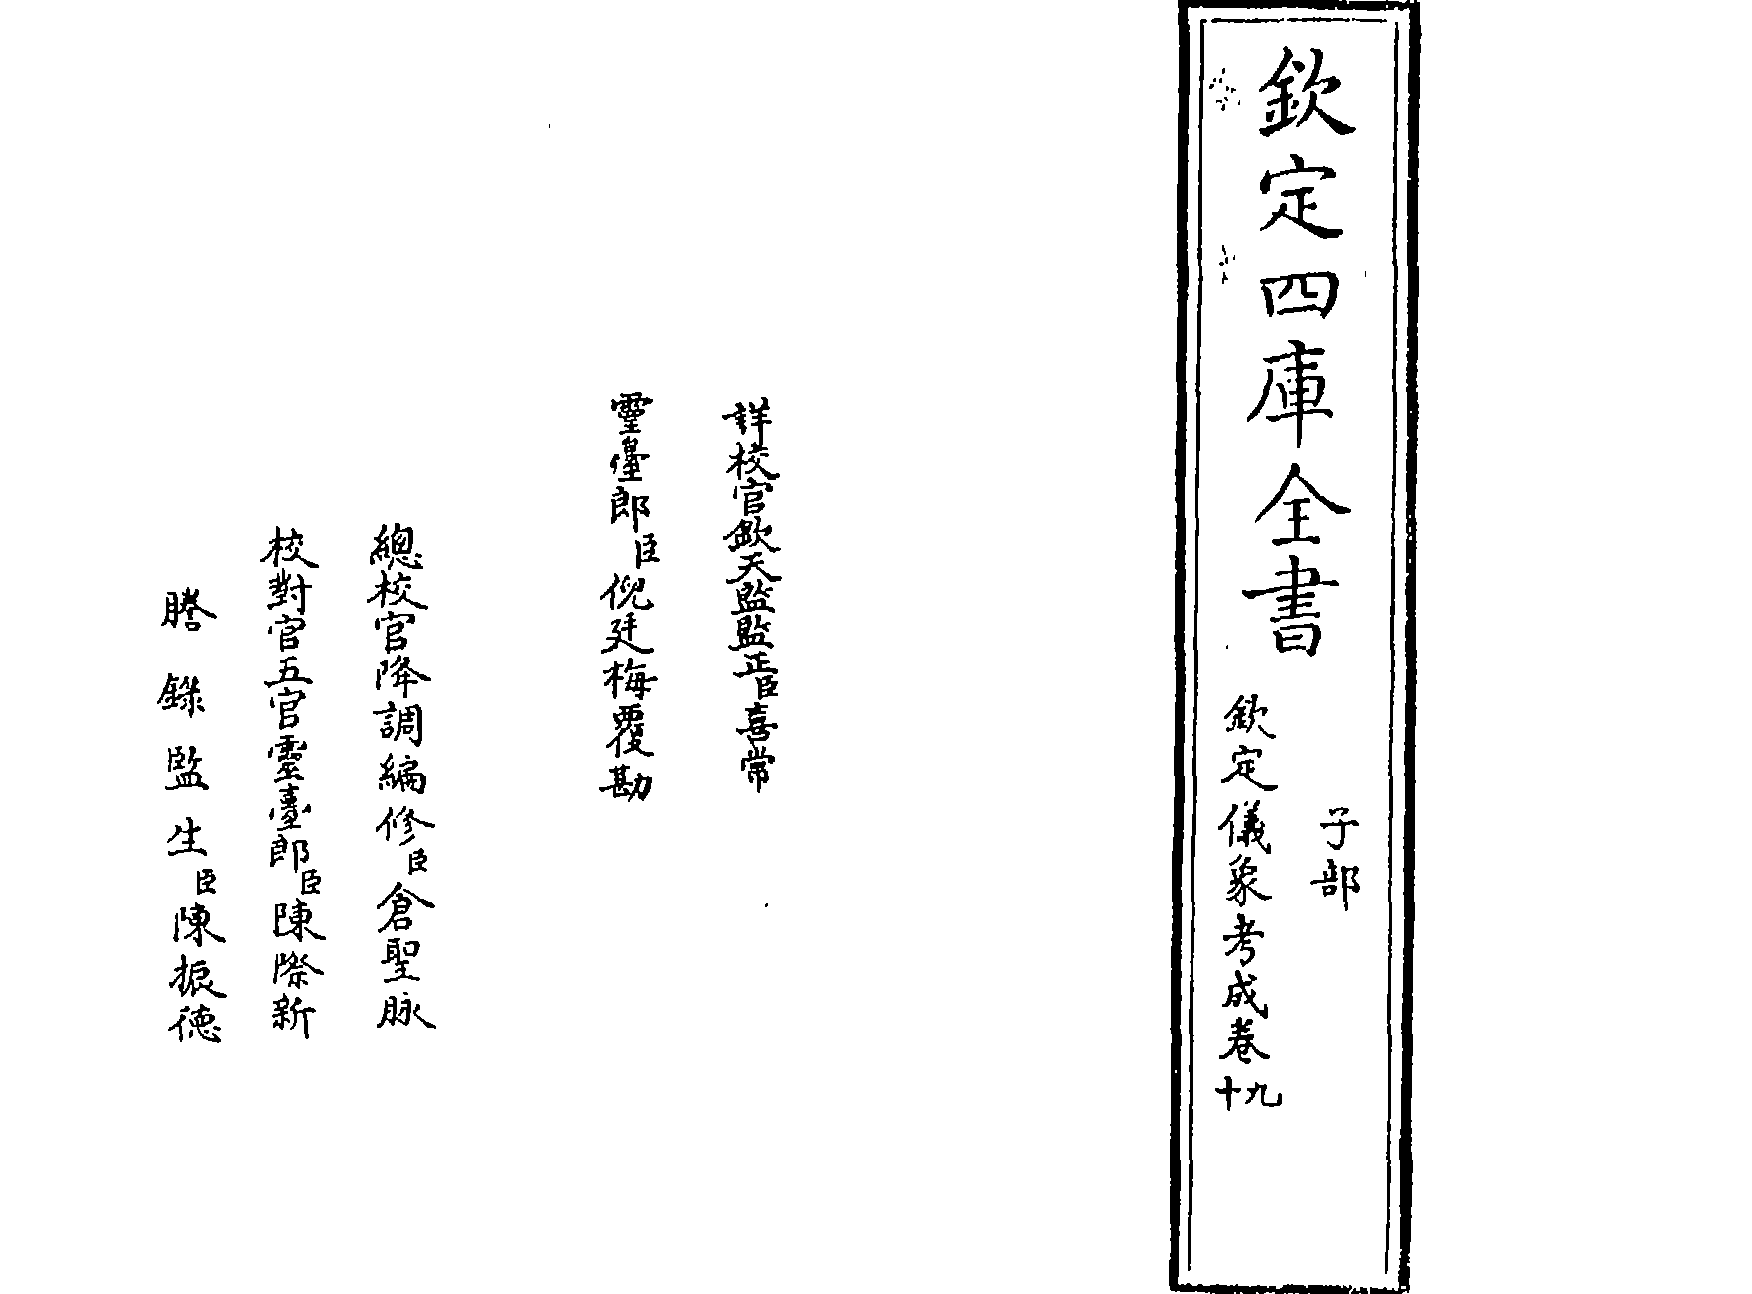
\includegraphics[width=\paperwidth,height=\paperheight,keepaspectratio]{img/0804.png}\clearpage
\begin{正文}
% ---- 册793 葉805 ----
\SetPageNumber{1}
欽定四庫全書\换行
欽定儀象考成卷九\换行
　恒星黄道經緯度表八\换行
　　黄道鶉火宫\双列{\右小列{赤道度附}\左小列{}}\换行
\char"200B\relax\换行
\char"200B\relax\换行
\char"200B\relax\换行
\char"200B\relax\换行
\char"200B\relax\换行
\char"200B\relax\换行
\char"200B\relax\换行
\char"200B\relax\换行
\char"200B\relax\换行
\char"200B\relax\换行
\char"200B\relax\换行
\char"200B\relax
\par
\end{正文}\clearpage
\嵌图{142.64pt}{201.94pt}{846.47pt}{585.91pt}{img/0808.png}
\begin{正文}
% ---- 册793 葉808 图版 ----
\SetPageNumber{2}
\插图页
\char"200B\relax\换行
\char"200B\relax\换行
\char"200B\relax\换行
\char"200B\relax\换行
\char"200B\relax\换行
\char"200B\relax\换行
\char"200B\relax\换行
\char"200B\relax\换行
\char"200B\relax\换行
\char"200B\relax\换行
\char"200B\relax\换行
\char"200B\relax\换行
\char"200B\relax\换行
\char"200B\relax\换行
\char"200B\relax\换行
\char"200B\relax
\恢复丝栏\par
\end{正文}\clearpage
\嵌图{144.63pt}{201.45pt}{842.50pt}{586.89pt}{img/0809.png}
\begin{正文}
% ---- 册793 葉809 图版 ----
\SetPageNumber{3}
\插图页
\char"200B\relax\换行
\char"200B\relax\换行
\char"200B\relax\换行
\char"200B\relax\换行
\char"200B\relax\换行
\char"200B\relax\换行
\char"200B\relax\换行
\char"200B\relax\换行
\char"200B\relax\换行
\char"200B\relax\换行
\char"200B\relax\换行
\char"200B\relax\换行
\char"200B\relax\换行
\char"200B\relax\换行
\char"200B\relax\换行
\char"200B\relax
\恢复丝栏\par
\end{正文}\clearpage
\嵌图{142.64pt}{201.00pt}{846.47pt}{587.79pt}{img/0812.png}
\begin{正文}
% ---- 册793 葉812 图版 ----
\SetPageNumber{4}
\插图页
\char"200B\relax\换行
\char"200B\relax\换行
\char"200B\relax\换行
\char"200B\relax\换行
\char"200B\relax\换行
\char"200B\relax\换行
\char"200B\relax\换行
\char"200B\relax\换行
\char"200B\relax\换行
\char"200B\relax\换行
\char"200B\relax\换行
\char"200B\relax\换行
\char"200B\relax\换行
\char"200B\relax\换行
\char"200B\relax\换行
\char"200B\relax
\恢复丝栏\par
\end{正文}\clearpage
\嵌图{148.61pt}{202.84pt}{834.55pt}{584.11pt}{img/0813.png}
\begin{正文}
% ---- 册793 葉813 图版 ----
\SetPageNumber{5}
\插图页
\char"200B\relax\换行
\char"200B\relax\换行
\char"200B\relax\换行
\char"200B\relax\换行
\char"200B\relax\换行
\char"200B\relax\换行
\char"200B\relax\换行
\char"200B\relax\换行
\char"200B\relax\换行
\char"200B\relax\换行
\char"200B\relax\换行
\char"200B\relax\换行
\char"200B\relax\换行
\char"200B\relax\换行
\char"200B\relax\换行
\char"200B\relax
\恢复丝栏\par
\end{正文}\clearpage
\嵌图{144.72pt}{202.49pt}{842.31pt}{584.82pt}{img/0816.png}
\begin{正文}
% ---- 册793 葉816 图版 ----
\SetPageNumber{6}
\插图页
\char"200B\relax\换行
\char"200B\relax\换行
\char"200B\relax\换行
\char"200B\relax\换行
\char"200B\relax\换行
\char"200B\relax\换行
\char"200B\relax\换行
\char"200B\relax\换行
\char"200B\relax\换行
\char"200B\relax\换行
\char"200B\relax\换行
\char"200B\relax\换行
\char"200B\relax\换行
\char"200B\relax\换行
\char"200B\relax\换行
\char"200B\relax
\恢复丝栏\par
\end{正文}\clearpage
\嵌图{144.72pt}{201.04pt}{842.31pt}{587.70pt}{img/0817.png}
\begin{正文}
% ---- 册793 葉817 图版 ----
\SetPageNumber{7}
\插图页
\char"200B\relax\换行
\char"200B\relax\换行
\char"200B\relax\换行
\char"200B\relax\换行
\char"200B\relax\换行
\char"200B\relax\换行
\char"200B\relax\换行
\char"200B\relax\换行
\char"200B\relax\换行
\char"200B\relax\换行
\char"200B\relax\换行
\char"200B\relax\换行
\char"200B\relax\换行
\char"200B\relax\换行
\char"200B\relax\换行
\char"200B\relax
\恢复丝栏\par
\end{正文}\clearpage
\嵌图{144.63pt}{200.98pt}{842.50pt}{587.83pt}{img/0820.png}
\begin{正文}
% ---- 册793 葉820 图版 ----
\SetPageNumber{8}
\插图页
\char"200B\relax\换行
\char"200B\relax\换行
\char"200B\relax\换行
\char"200B\relax\换行
\char"200B\relax\换行
\char"200B\relax\换行
\char"200B\relax\换行
\char"200B\relax\换行
\char"200B\relax\换行
\char"200B\relax\换行
\char"200B\relax\换行
\char"200B\relax\换行
\char"200B\relax\换行
\char"200B\relax\换行
\char"200B\relax\换行
\char"200B\relax
\恢复丝栏\par
\end{正文}\clearpage
\嵌图{144.63pt}{200.96pt}{842.50pt}{587.87pt}{img/0821.png}
\begin{正文}
% ---- 册793 葉821 图版 ----
\SetPageNumber{9}
\插图页
\char"200B\relax\换行
\char"200B\relax\换行
\char"200B\relax\换行
\char"200B\relax\换行
\char"200B\relax\换行
\char"200B\relax\换行
\char"200B\relax\换行
\char"200B\relax\换行
\char"200B\relax\换行
\char"200B\relax\换行
\char"200B\relax\换行
\char"200B\relax\换行
\char"200B\relax\换行
\char"200B\relax\换行
\char"200B\relax\换行
\char"200B\relax
\恢复丝栏\par
\end{正文}\clearpage
\嵌图{144.68pt}{202.94pt}{842.41pt}{583.90pt}{img/0824.png}
\begin{正文}
% ---- 册793 葉824 图版 ----
\SetPageNumber{10}
\插图页
\char"200B\relax\换行
\char"200B\relax\换行
\char"200B\relax\换行
\char"200B\relax\换行
\char"200B\relax\换行
\char"200B\relax\换行
\char"200B\relax\换行
\char"200B\relax\换行
\char"200B\relax\换行
\char"200B\relax\换行
\char"200B\relax\换行
\char"200B\relax\换行
\char"200B\relax\换行
\char"200B\relax\换行
\char"200B\relax\换行
\char"200B\relax
\恢复丝栏\par
\end{正文}\clearpage
\嵌图{144.68pt}{201.98pt}{842.41pt}{585.83pt}{img/0825.png}
\begin{正文}
% ---- 册793 葉825 图版 ----
\SetPageNumber{11}
\插图页
\char"200B\relax\换行
\char"200B\relax\换行
\char"200B\relax\换行
\char"200B\relax\换行
\char"200B\relax\换行
\char"200B\relax\换行
\char"200B\relax\换行
\char"200B\relax\换行
\char"200B\relax\换行
\char"200B\relax\换行
\char"200B\relax\换行
\char"200B\relax\换行
\char"200B\relax\换行
\char"200B\relax\换行
\char"200B\relax\换行
\char"200B\relax
\恢复丝栏\par
\end{正文}\clearpage
\嵌图{144.68pt}{202.94pt}{842.41pt}{583.92pt}{img/0828.png}
\begin{正文}
% ---- 册793 葉828 图版 ----
\SetPageNumber{12}
\插图页
\char"200B\relax\换行
\char"200B\relax\换行
\char"200B\relax\换行
\char"200B\relax\换行
\char"200B\relax\换行
\char"200B\relax\换行
\char"200B\relax\换行
\char"200B\relax\换行
\char"200B\relax\换行
\char"200B\relax\换行
\char"200B\relax\换行
\char"200B\relax\换行
\char"200B\relax\换行
\char"200B\relax\换行
\char"200B\relax\换行
\char"200B\relax
\恢复丝栏\par
\end{正文}\clearpage
\嵌图{144.68pt}{200.04pt}{842.41pt}{589.71pt}{img/0829.png}
\begin{正文}
% ---- 册793 葉829 图版 ----
\SetPageNumber{13}
\插图页
\char"200B\relax\换行
\char"200B\relax\换行
\char"200B\relax\换行
\char"200B\relax\换行
\char"200B\relax\换行
\char"200B\relax\换行
\char"200B\relax\换行
\char"200B\relax\换行
\char"200B\relax\换行
\char"200B\relax\换行
\char"200B\relax\换行
\char"200B\relax\换行
\char"200B\relax\换行
\char"200B\relax\换行
\char"200B\relax\换行
\char"200B\relax
\恢复丝栏\par
\end{正文}\clearpage
\嵌图{144.63pt}{202.94pt}{842.50pt}{583.92pt}{img/0832.png}
\begin{正文}
% ---- 册793 葉832 图版 ----
\SetPageNumber{14}
\插图页
\char"200B\relax\换行
\char"200B\relax\换行
\char"200B\relax\换行
\char"200B\relax\换行
\char"200B\relax\换行
\char"200B\relax\换行
\char"200B\relax\换行
\char"200B\relax\换行
\char"200B\relax\换行
\char"200B\relax\换行
\char"200B\relax\换行
\char"200B\relax\换行
\char"200B\relax\换行
\char"200B\relax\换行
\char"200B\relax\换行
\char"200B\relax
\恢复丝栏\par
\end{正文}\clearpage
\嵌图{144.63pt}{200.51pt}{842.50pt}{588.76pt}{img/0833.png}
\begin{正文}
% ---- 册793 葉833 图版 ----
\SetPageNumber{15}
\插图页
\char"200B\relax\换行
\char"200B\relax\换行
\char"200B\relax\换行
\char"200B\relax\换行
\char"200B\relax\换行
\char"200B\relax\换行
\char"200B\relax\换行
\char"200B\relax\换行
\char"200B\relax\换行
\char"200B\relax\换行
\char"200B\relax\换行
\char"200B\relax\换行
\char"200B\relax\换行
\char"200B\relax\换行
\char"200B\relax\换行
\char"200B\relax
\恢复丝栏\par
\end{正文}\clearpage
\嵌图{144.63pt}{201.51pt}{842.50pt}{586.77pt}{img/0836.png}
\begin{正文}
% ---- 册793 葉836 图版 ----
\SetPageNumber{16}
\插图页
\char"200B\relax\换行
\char"200B\relax\换行
\char"200B\relax\换行
\char"200B\relax\换行
\char"200B\relax\换行
\char"200B\relax\换行
\char"200B\relax\换行
\char"200B\relax\换行
\char"200B\relax\换行
\char"200B\relax\换行
\char"200B\relax\换行
\char"200B\relax\换行
\char"200B\relax\换行
\char"200B\relax\换行
\char"200B\relax\换行
\char"200B\relax
\恢复丝栏\par
\end{正文}\clearpage
\嵌图{146.62pt}{201.91pt}{838.53pt}{585.98pt}{img/0837.png}
\begin{正文}
% ---- 册793 葉837 图版 ----
\SetPageNumber{17}
\插图页
\char"200B\relax\换行
\char"200B\relax\换行
\char"200B\relax\换行
\char"200B\relax\换行
\char"200B\relax\换行
\char"200B\relax\换行
\char"200B\relax\换行
\char"200B\relax\换行
\char"200B\relax\换行
\char"200B\relax\换行
\char"200B\relax\换行
\char"200B\relax\换行
\char"200B\relax\换行
\char"200B\relax\换行
\char"200B\relax\换行
\char"200B\relax
\恢复丝栏\par
\end{正文}\clearpage
\嵌图{142.64pt}{201.50pt}{846.47pt}{586.78pt}{img/0840.png}
\begin{正文}
% ---- 册793 葉840 图版 ----
\SetPageNumber{18}
\插图页
\char"200B\relax\换行
\char"200B\relax\换行
\char"200B\relax\换行
\char"200B\relax\换行
\char"200B\relax\换行
\char"200B\relax\换行
\char"200B\relax\换行
\char"200B\relax\换行
\char"200B\relax\换行
\char"200B\relax\换行
\char"200B\relax\换行
\char"200B\relax\换行
\char"200B\relax\换行
\char"200B\relax\换行
\char"200B\relax\换行
\char"200B\relax
\恢复丝栏\par
\end{正文}\clearpage
\嵌图{142.64pt}{201.01pt}{846.47pt}{587.77pt}{img/0841.png}
\begin{正文}
% ---- 册793 葉841 图版 ----
\SetPageNumber{19}
\插图页
\char"200B\relax\换行
\char"200B\relax\换行
\char"200B\relax\换行
\char"200B\relax\换行
\char"200B\relax\换行
\char"200B\relax\换行
\char"200B\relax\换行
\char"200B\relax\换行
\char"200B\relax\换行
\char"200B\relax\换行
\char"200B\relax\换行
\char"200B\relax\换行
\char"200B\relax\换行
\char"200B\relax\换行
\char"200B\relax\换行
\char"200B\relax
\恢复丝栏\par
\end{正文}\clearpage
\嵌图{146.62pt}{200.02pt}{838.53pt}{589.74pt}{img/0844.png}
\begin{正文}
% ---- 册793 葉844 图版 ----
\SetPageNumber{20}
\插图页
\char"200B\relax\换行
\char"200B\relax\换行
\char"200B\relax\换行
\char"200B\relax\换行
\char"200B\relax\换行
\char"200B\relax\换行
\char"200B\relax\换行
\char"200B\relax\换行
\char"200B\relax\换行
\char"200B\relax\换行
\char"200B\relax\换行
\char"200B\relax\换行
\char"200B\relax\换行
\char"200B\relax\换行
\char"200B\relax\换行
\char"200B\relax
\恢复丝栏\par
\end{正文}\clearpage
\嵌图{142.64pt}{202.82pt}{846.47pt}{584.14pt}{img/0845.png}
\begin{正文}
% ---- 册793 葉845 图版 ----
\SetPageNumber{21}
\插图页
\char"200B\relax\换行
\char"200B\relax\换行
\char"200B\relax\换行
\char"200B\relax\换行
\char"200B\relax\换行
\char"200B\relax\换行
\char"200B\relax\换行
\char"200B\relax\换行
\char"200B\relax\换行
\char"200B\relax\换行
\char"200B\relax\换行
\char"200B\relax\换行
\char"200B\relax\换行
\char"200B\relax\换行
\char"200B\relax\换行
\char"200B\relax
\恢复丝栏\par
\end{正文}\clearpage
\嵌图{146.62pt}{201.02pt}{838.53pt}{587.76pt}{img/0848.png}
\begin{正文}
% ---- 册793 葉848 图版 ----
\SetPageNumber{22}
\插图页
\char"200B\relax\换行
\char"200B\relax\换行
\char"200B\relax\换行
\char"200B\relax\换行
\char"200B\relax\换行
\char"200B\relax\换行
\char"200B\relax\换行
\char"200B\relax\换行
\char"200B\relax\换行
\char"200B\relax\换行
\char"200B\relax\换行
\char"200B\relax\换行
\char"200B\relax\换行
\char"200B\relax\换行
\char"200B\relax\换行
\char"200B\relax
\恢复丝栏\par
\end{正文}\clearpage
\嵌图{142.64pt}{199.59pt}{846.47pt}{590.61pt}{img/0849.png}
\begin{正文}
% ---- 册793 葉849 图版 ----
\SetPageNumber{23}
\插图页
\char"200B\relax\换行
\char"200B\relax\换行
\char"200B\relax\换行
\char"200B\relax\换行
\char"200B\relax\换行
\char"200B\relax\换行
\char"200B\relax\换行
\char"200B\relax\换行
\char"200B\relax\换行
\char"200B\relax\换行
\char"200B\relax\换行
\char"200B\relax\换行
\char"200B\relax\换行
\char"200B\relax\换行
\char"200B\relax\换行
\char"200B\relax
\恢复丝栏\par
\end{正文}\clearpage
\嵌图{150.30pt}{198.15pt}{831.15pt}{593.49pt}{img/0852.png}
\begin{正文}
% ---- 册793 葉852 图版 ----
\SetPageNumber{24}
\插图页
\char"200B\relax\换行
\char"200B\relax\换行
\char"200B\relax\换行
\char"200B\relax\换行
\char"200B\relax\换行
\char"200B\relax\换行
\char"200B\relax\换行
\char"200B\relax\换行
\char"200B\relax\换行
\char"200B\relax\换行
\char"200B\relax\换行
\char"200B\relax\换行
\char"200B\relax\换行
\char"200B\relax\换行
\char"200B\relax\换行
\char"200B\relax
\恢复丝栏\par
\end{正文}\clearpage
\嵌图{150.93pt}{209.28pt}{397.09pt}{583.55pt}{img/0853.png}
\begin{正文}
% ---- 册793 葉853 ----
\SetPageNumber{25}
\插图页
\char"200B\relax\换行
\char"200B\relax\换行
\char"200B\relax\换行
\char"200B\relax\换行
\char"200B\relax\换行
\char"200B\relax\换行
\char"200B\relax\换行
\char"200B\relax\换行
\恢复丝栏
\char"200B\relax\换行
\char"200B\relax\换行
\char"200B\relax\换行
\char"200B\relax\换行
\char"200B\relax\换行
\char"200B\relax\换行
\char"200B\relax\换行
欽定儀象考成卷九
\par

% ======== 卷十（8行21字）========
\par\end{正文}\clearpage
\chapter*{欽定儀象考成卷十}
\begin{正文}
% ---- 册793 葉856 ----
\SetPageNumber{1}
欽定四庫全書\换行
欽定儀象考成卷十\换行
　恒星黄道經緯度表九\换行
　　黄道鶉尾宫\双列{\右小列{赤道度附}\左小列{}}\换行
\char"200B\relax\换行
\char"200B\relax\换行
\char"200B\relax\换行
\char"200B\relax\换行
\char"200B\relax\换行
\char"200B\relax\换行
\char"200B\relax\换行
\char"200B\relax\换行
\char"200B\relax\换行
\char"200B\relax\换行
\char"200B\relax\换行
\char"200B\relax
\par
\end{正文}\clearpage
\嵌图{144.63pt}{201.50pt}{842.50pt}{586.80pt}{img/0857.png}
\begin{正文}
% ---- 册793 葉857 图版 ----
\SetPageNumber{2}
\插图页
\char"200B\relax\换行
\char"200B\relax\换行
\char"200B\relax\换行
\char"200B\relax\换行
\char"200B\relax\换行
\char"200B\relax\换行
\char"200B\relax\换行
\char"200B\relax\换行
\char"200B\relax\换行
\char"200B\relax\换行
\char"200B\relax\换行
\char"200B\relax\换行
\char"200B\relax\换行
\char"200B\relax\换行
\char"200B\relax\换行
\char"200B\relax
\恢复丝栏\par
\end{正文}\clearpage
\嵌图{144.63pt}{201.53pt}{842.50pt}{586.74pt}{img/0860.png}
\begin{正文}
% ---- 册793 葉860 图版 ----
\SetPageNumber{3}
\插图页
\char"200B\relax\换行
\char"200B\relax\换行
\char"200B\relax\换行
\char"200B\relax\换行
\char"200B\relax\换行
\char"200B\relax\换行
\char"200B\relax\换行
\char"200B\relax\换行
\char"200B\relax\换行
\char"200B\relax\换行
\char"200B\relax\换行
\char"200B\relax\换行
\char"200B\relax\换行
\char"200B\relax\换行
\char"200B\relax\换行
\char"200B\relax
\恢复丝栏\par
\end{正文}\clearpage
\嵌图{146.62pt}{201.46pt}{838.53pt}{586.87pt}{img/0861.png}
\begin{正文}
% ---- 册793 葉861 图版 ----
\SetPageNumber{4}
\插图页
\char"200B\relax\换行
\char"200B\relax\换行
\char"200B\relax\换行
\char"200B\relax\换行
\char"200B\relax\换行
\char"200B\relax\换行
\char"200B\relax\换行
\char"200B\relax\换行
\char"200B\relax\换行
\char"200B\relax\换行
\char"200B\relax\换行
\char"200B\relax\换行
\char"200B\relax\换行
\char"200B\relax\换行
\char"200B\relax\换行
\char"200B\relax
\恢复丝栏\par
\end{正文}\clearpage
\嵌图{146.56pt}{201.05pt}{838.64pt}{587.69pt}{img/0864.png}
\begin{正文}
% ---- 册793 葉864 图版 ----
\SetPageNumber{5}
\插图页
\char"200B\relax\换行
\char"200B\relax\换行
\char"200B\relax\换行
\char"200B\relax\换行
\char"200B\relax\换行
\char"200B\relax\换行
\char"200B\relax\换行
\char"200B\relax\换行
\char"200B\relax\换行
\char"200B\relax\换行
\char"200B\relax\换行
\char"200B\relax\换行
\char"200B\relax\换行
\char"200B\relax\换行
\char"200B\relax\换行
\char"200B\relax
\恢复丝栏\par
\end{正文}\clearpage
\嵌图{146.56pt}{201.50pt}{838.64pt}{586.78pt}{img/0865.png}
\begin{正文}
% ---- 册793 葉865 图版 ----
\SetPageNumber{6}
\插图页
\char"200B\relax\换行
\char"200B\relax\换行
\char"200B\relax\换行
\char"200B\relax\换行
\char"200B\relax\换行
\char"200B\relax\换行
\char"200B\relax\换行
\char"200B\relax\换行
\char"200B\relax\换行
\char"200B\relax\换行
\char"200B\relax\换行
\char"200B\relax\换行
\char"200B\relax\换行
\char"200B\relax\换行
\char"200B\relax\换行
\char"200B\relax
\恢复丝栏\par
\end{正文}\clearpage
\嵌图{144.63pt}{200.09pt}{842.50pt}{589.60pt}{img/0868.png}
\begin{正文}
% ---- 册793 葉868 图版 ----
\SetPageNumber{7}
\插图页
\char"200B\relax\换行
\char"200B\relax\换行
\char"200B\relax\换行
\char"200B\relax\换行
\char"200B\relax\换行
\char"200B\relax\换行
\char"200B\relax\换行
\char"200B\relax\换行
\char"200B\relax\换行
\char"200B\relax\换行
\char"200B\relax\换行
\char"200B\relax\换行
\char"200B\relax\换行
\char"200B\relax\换行
\char"200B\relax\换行
\char"200B\relax
\恢复丝栏\par
\end{正文}\clearpage
\嵌图{146.62pt}{200.51pt}{838.53pt}{588.76pt}{img/0869.png}
\begin{正文}
% ---- 册793 葉869 图版 ----
\SetPageNumber{8}
\插图页
\char"200B\relax\换行
\char"200B\relax\换行
\char"200B\relax\换行
\char"200B\relax\换行
\char"200B\relax\换行
\char"200B\relax\换行
\char"200B\relax\换行
\char"200B\relax\换行
\char"200B\relax\换行
\char"200B\relax\换行
\char"200B\relax\换行
\char"200B\relax\换行
\char"200B\relax\换行
\char"200B\relax\换行
\char"200B\relax\换行
\char"200B\relax
\恢复丝栏\par
\end{正文}\clearpage
\嵌图{144.63pt}{199.14pt}{842.50pt}{591.50pt}{img/0872.png}
\begin{正文}
% ---- 册793 葉872 图版 ----
\SetPageNumber{9}
\插图页
\char"200B\relax\换行
\char"200B\relax\换行
\char"200B\relax\换行
\char"200B\relax\换行
\char"200B\relax\换行
\char"200B\relax\换行
\char"200B\relax\换行
\char"200B\relax\换行
\char"200B\relax\换行
\char"200B\relax\换行
\char"200B\relax\换行
\char"200B\relax\换行
\char"200B\relax\换行
\char"200B\relax\换行
\char"200B\relax\换行
\char"200B\relax
\恢复丝栏\par
\end{正文}\clearpage
\嵌图{146.62pt}{201.49pt}{838.53pt}{586.81pt}{img/0873.png}
\begin{正文}
% ---- 册793 葉873 图版 ----
\SetPageNumber{10}
\插图页
\char"200B\relax\换行
\char"200B\relax\换行
\char"200B\relax\换行
\char"200B\relax\换行
\char"200B\relax\换行
\char"200B\relax\换行
\char"200B\relax\换行
\char"200B\relax\换行
\char"200B\relax\换行
\char"200B\relax\换行
\char"200B\relax\换行
\char"200B\relax\换行
\char"200B\relax\换行
\char"200B\relax\换行
\char"200B\relax\换行
\char"200B\relax
\恢复丝栏\par
\end{正文}\clearpage
\嵌图{144.63pt}{200.51pt}{842.50pt}{588.77pt}{img/0876.png}
\begin{正文}
% ---- 册793 葉876 图版 ----
\SetPageNumber{11}
\插图页
\char"200B\relax\换行
\char"200B\relax\换行
\char"200B\relax\换行
\char"200B\relax\换行
\char"200B\relax\换行
\char"200B\relax\换行
\char"200B\relax\换行
\char"200B\relax\换行
\char"200B\relax\换行
\char"200B\relax\换行
\char"200B\relax\换行
\char"200B\relax\换行
\char"200B\relax\换行
\char"200B\relax\换行
\char"200B\relax\换行
\char"200B\relax
\恢复丝栏\par
\end{正文}\clearpage
\嵌图{146.62pt}{199.08pt}{838.53pt}{591.64pt}{img/0877.png}
\begin{正文}
% ---- 册793 葉877 图版 ----
\SetPageNumber{12}
\插图页
\char"200B\relax\换行
\char"200B\relax\换行
\char"200B\relax\换行
\char"200B\relax\换行
\char"200B\relax\换行
\char"200B\relax\换行
\char"200B\relax\换行
\char"200B\relax\换行
\char"200B\relax\换行
\char"200B\relax\换行
\char"200B\relax\换行
\char"200B\relax\换行
\char"200B\relax\换行
\char"200B\relax\换行
\char"200B\relax\换行
\char"200B\relax
\恢复丝栏\par
\end{正文}\clearpage
\嵌图{142.68pt}{201.00pt}{846.40pt}{587.79pt}{img/0880.png}
\begin{正文}
% ---- 册793 葉880 图版 ----
\SetPageNumber{13}
\插图页
\char"200B\relax\换行
\char"200B\relax\换行
\char"200B\relax\换行
\char"200B\relax\换行
\char"200B\relax\换行
\char"200B\relax\换行
\char"200B\relax\换行
\char"200B\relax\换行
\char"200B\relax\换行
\char"200B\relax\换行
\char"200B\relax\换行
\char"200B\relax\换行
\char"200B\relax\换行
\char"200B\relax\换行
\char"200B\relax\换行
\char"200B\relax
\恢复丝栏\par
\end{正文}\clearpage
\嵌图{142.68pt}{201.96pt}{846.40pt}{585.86pt}{img/0881.png}
\begin{正文}
% ---- 册793 葉881 图版 ----
\SetPageNumber{14}
\插图页
\char"200B\relax\换行
\char"200B\relax\换行
\char"200B\relax\换行
\char"200B\relax\换行
\char"200B\relax\换行
\char"200B\relax\换行
\char"200B\relax\换行
\char"200B\relax\换行
\char"200B\relax\换行
\char"200B\relax\换行
\char"200B\relax\换行
\char"200B\relax\换行
\char"200B\relax\换行
\char"200B\relax\换行
\char"200B\relax\换行
\char"200B\relax
\恢复丝栏\par
\end{正文}\clearpage
\嵌图{144.63pt}{200.51pt}{842.50pt}{588.76pt}{img/0884.png}
\begin{正文}
% ---- 册793 葉884 图版 ----
\SetPageNumber{15}
\插图页
\char"200B\relax\换行
\char"200B\relax\换行
\char"200B\relax\换行
\char"200B\relax\换行
\char"200B\relax\换行
\char"200B\relax\换行
\char"200B\relax\换行
\char"200B\relax\换行
\char"200B\relax\换行
\char"200B\relax\换行
\char"200B\relax\换行
\char"200B\relax\换行
\char"200B\relax\换行
\char"200B\relax\换行
\char"200B\relax\换行
\char"200B\relax
\恢复丝栏\par
\end{正文}\clearpage
\嵌图{146.62pt}{201.91pt}{838.53pt}{585.98pt}{img/0885.png}
\begin{正文}
% ---- 册793 葉885 图版 ----
\SetPageNumber{16}
\插图页
\char"200B\relax\换行
\char"200B\relax\换行
\char"200B\relax\换行
\char"200B\relax\换行
\char"200B\relax\换行
\char"200B\relax\换行
\char"200B\relax\换行
\char"200B\relax\换行
\char"200B\relax\换行
\char"200B\relax\换行
\char"200B\relax\换行
\char"200B\relax\换行
\char"200B\relax\换行
\char"200B\relax\换行
\char"200B\relax\换行
\char"200B\relax
\恢复丝栏\par
\end{正文}\clearpage
\嵌图{144.63pt}{200.54pt}{842.50pt}{588.71pt}{img/0888.png}
\begin{正文}
% ---- 册793 葉888 图版 ----
\SetPageNumber{17}
\插图页
\char"200B\relax\换行
\char"200B\relax\换行
\char"200B\relax\换行
\char"200B\relax\换行
\char"200B\relax\换行
\char"200B\relax\换行
\char"200B\relax\换行
\char"200B\relax\换行
\char"200B\relax\换行
\char"200B\relax\换行
\char"200B\relax\换行
\char"200B\relax\换行
\char"200B\relax\换行
\char"200B\relax\换行
\char"200B\relax\换行
\char"200B\relax
\恢复丝栏\par
\end{正文}\clearpage
\嵌图{144.63pt}{198.65pt}{842.50pt}{592.48pt}{img/0889.png}
\begin{正文}
% ---- 册793 葉889 图版 ----
\SetPageNumber{18}
\插图页
\char"200B\relax\换行
\char"200B\relax\换行
\char"200B\relax\换行
\char"200B\relax\换行
\char"200B\relax\换行
\char"200B\relax\换行
\char"200B\relax\换行
\char"200B\relax\换行
\char"200B\relax\换行
\char"200B\relax\换行
\char"200B\relax\换行
\char"200B\relax\换行
\char"200B\relax\换行
\char"200B\relax\换行
\char"200B\relax\换行
\char"200B\relax
\恢复丝栏\par
\end{正文}\clearpage
\嵌图{145.26pt}{209.32pt}{402.76pt}{583.51pt}{img/0892.png}
\begin{正文}
% ---- 册793 葉892 ----
\SetPageNumber{19}
\插图页
\char"200B\relax\换行
\char"200B\relax\换行
\char"200B\relax\换行
\char"200B\relax\换行
\char"200B\relax\换行
\char"200B\relax\换行
\char"200B\relax\换行
\char"200B\relax\换行
\恢复丝栏
\char"200B\relax\换行
\char"200B\relax\换行
\char"200B\relax\换行
\char"200B\relax\换行
\char"200B\relax\换行
\char"200B\relax\换行
欽定儀象考成卷十\换行
\char"200B\relax
\par

% ======== 卷十一（8行21字）========
\par\end{正文}\clearpage
\chapter*{欽定儀象考成卷十一}
\begin{正文}
\end{正文}\clearpage

  % ======== 卷十四（8行21字）========
\chapter*{欽定儀象考成卷十四}
\begin{正文}
\end{正文}\clearpage
\thispagestyle{empty}\noindent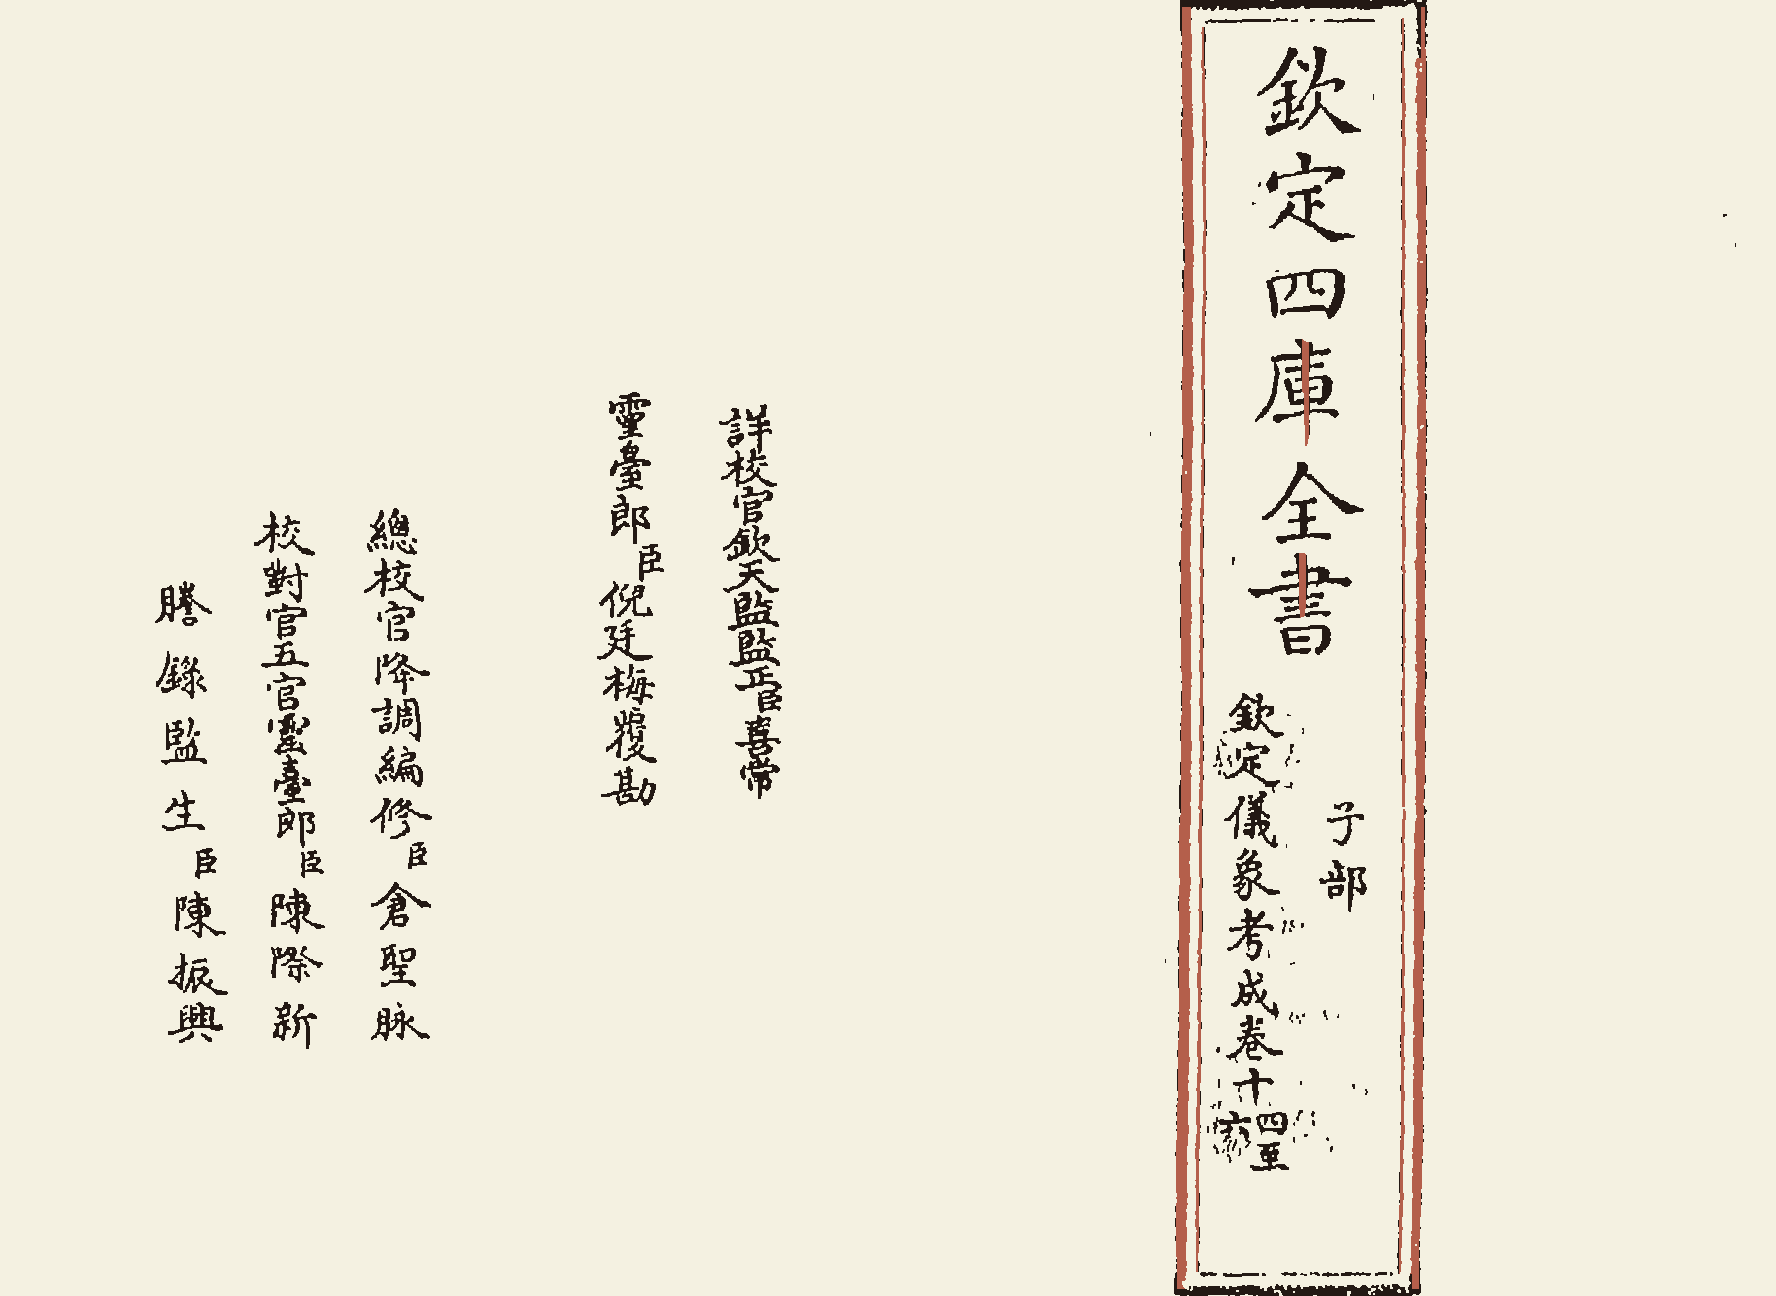
\includegraphics[width=\paperwidth,height=\paperheight,keepaspectratio]{img/1012.png}\clearpage
\begin{正文}
% ---- 册793 葉1013 ----
\SetPageNumber{1}
欽定四庫全書\换行
欽定儀象考成卷十四\换行
　恒星赤道經緯度表一\换行
　　赤道星紀宫\双列{\右小列{黄道度附}\左小列{}}\换行
\char"200B\relax\换行
\char"200B\relax\换行
\char"200B\relax\换行
\char"200B\relax\换行
\char"200B\relax\换行
\char"200B\relax\换行
\char"200B\relax\换行
\char"200B\relax\换行
\char"200B\relax\换行
\char"200B\relax\换行
\char"200B\relax\换行
\char"200B\relax
\par
\end{正文}\clearpage
\嵌图{142.64pt}{200.54pt}{846.47pt}{588.72pt}{img/1016.png}
\begin{正文}
% ---- 册793 葉1016 图版 ----
\SetPageNumber{2}
\插图页
\char"200B\relax\换行
\char"200B\relax\换行
\char"200B\relax\换行
\char"200B\relax\换行
\char"200B\relax\换行
\char"200B\relax\换行
\char"200B\relax\换行
\char"200B\relax\换行
\char"200B\relax\换行
\char"200B\relax\换行
\char"200B\relax\换行
\char"200B\relax\换行
\char"200B\relax\换行
\char"200B\relax\换行
\char"200B\relax\换行
\char"200B\relax
\恢复丝栏\par
\end{正文}\clearpage
\嵌图{148.61pt}{201.49pt}{834.55pt}{586.81pt}{img/1017.png}
\begin{正文}
% ---- 册793 葉1017 图版 ----
\SetPageNumber{3}
\插图页
\char"200B\relax\换行
\char"200B\relax\换行
\char"200B\relax\换行
\char"200B\relax\换行
\char"200B\relax\换行
\char"200B\relax\换行
\char"200B\relax\换行
\char"200B\relax\换行
\char"200B\relax\换行
\char"200B\relax\换行
\char"200B\relax\换行
\char"200B\relax\换行
\char"200B\relax\换行
\char"200B\relax\换行
\char"200B\relax\换行
\char"200B\relax
\恢复丝栏\par
\end{正文}\clearpage
\嵌图{142.72pt}{201.96pt}{846.33pt}{585.86pt}{img/1020.png}
\begin{正文}
% ---- 册793 葉1020 图版 ----
\SetPageNumber{4}
\插图页
\char"200B\relax\换行
\char"200B\relax\换行
\char"200B\relax\换行
\char"200B\relax\换行
\char"200B\relax\换行
\char"200B\relax\换行
\char"200B\relax\换行
\char"200B\relax\换行
\char"200B\relax\换行
\char"200B\relax\换行
\char"200B\relax\换行
\char"200B\relax\换行
\char"200B\relax\换行
\char"200B\relax\换行
\char"200B\relax\换行
\char"200B\relax
\恢复丝栏\par
\end{正文}\clearpage
\嵌图{144.72pt}{201.47pt}{842.31pt}{586.86pt}{img/1021.png}
\begin{正文}
% ---- 册793 葉1021 图版 ----
\SetPageNumber{5}
\插图页
\char"200B\relax\换行
\char"200B\relax\换行
\char"200B\relax\换行
\char"200B\relax\换行
\char"200B\relax\换行
\char"200B\relax\换行
\char"200B\relax\换行
\char"200B\relax\换行
\char"200B\relax\换行
\char"200B\relax\换行
\char"200B\relax\换行
\char"200B\relax\换行
\char"200B\relax\换行
\char"200B\relax\换行
\char"200B\relax\换行
\char"200B\relax
\恢复丝栏\par
\end{正文}\clearpage
\嵌图{144.63pt}{200.06pt}{842.50pt}{589.67pt}{img/1024.png}
\begin{正文}
% ---- 册793 葉1024 图版 ----
\SetPageNumber{6}
\插图页
\char"200B\relax\换行
\char"200B\relax\换行
\char"200B\relax\换行
\char"200B\relax\换行
\char"200B\relax\换行
\char"200B\relax\换行
\char"200B\relax\换行
\char"200B\relax\换行
\char"200B\relax\换行
\char"200B\relax\换行
\char"200B\relax\换行
\char"200B\relax\换行
\char"200B\relax\换行
\char"200B\relax\换行
\char"200B\relax\换行
\char"200B\relax
\恢复丝栏\par
\end{正文}\clearpage
\嵌图{144.63pt}{200.54pt}{842.50pt}{588.72pt}{img/1025.png}
\begin{正文}
% ---- 册793 葉1025 图版 ----
\SetPageNumber{7}
\插图页
\char"200B\relax\换行
\char"200B\relax\换行
\char"200B\relax\换行
\char"200B\relax\换行
\char"200B\relax\换行
\char"200B\relax\换行
\char"200B\relax\换行
\char"200B\relax\换行
\char"200B\relax\换行
\char"200B\relax\换行
\char"200B\relax\换行
\char"200B\relax\换行
\char"200B\relax\换行
\char"200B\relax\换行
\char"200B\relax\换行
\char"200B\relax
\恢复丝栏\par
\end{正文}\clearpage
\嵌图{142.72pt}{201.01pt}{846.33pt}{587.77pt}{img/1028.png}
\begin{正文}
% ---- 册793 葉1028 图版 ----
\SetPageNumber{8}
\插图页
\char"200B\relax\换行
\char"200B\relax\换行
\char"200B\relax\换行
\char"200B\relax\换行
\char"200B\relax\换行
\char"200B\relax\换行
\char"200B\relax\换行
\char"200B\relax\换行
\char"200B\relax\换行
\char"200B\relax\换行
\char"200B\relax\换行
\char"200B\relax\换行
\char"200B\relax\换行
\char"200B\relax\换行
\char"200B\relax\换行
\char"200B\relax
\恢复丝栏\par
\end{正文}\clearpage
\嵌图{144.72pt}{200.98pt}{842.31pt}{587.83pt}{img/1029.png}
\begin{正文}
% ---- 册793 葉1029 图版 ----
\SetPageNumber{9}
\插图页
\char"200B\relax\换行
\char"200B\relax\换行
\char"200B\relax\换行
\char"200B\relax\换行
\char"200B\relax\换行
\char"200B\relax\换行
\char"200B\relax\换行
\char"200B\relax\换行
\char"200B\relax\换行
\char"200B\relax\换行
\char"200B\relax\换行
\char"200B\relax\换行
\char"200B\relax\换行
\char"200B\relax\换行
\char"200B\relax\换行
\char"200B\relax
\恢复丝栏\par
\end{正文}\clearpage
\嵌图{142.64pt}{200.06pt}{846.47pt}{589.67pt}{img/1032.png}
\begin{正文}
% ---- 册793 葉1032 图版 ----
\SetPageNumber{10}
\插图页
\char"200B\relax\换行
\char"200B\relax\换行
\char"200B\relax\换行
\char"200B\relax\换行
\char"200B\relax\换行
\char"200B\relax\换行
\char"200B\relax\换行
\char"200B\relax\换行
\char"200B\relax\换行
\char"200B\relax\换行
\char"200B\relax\换行
\char"200B\relax\换行
\char"200B\relax\换行
\char"200B\relax\换行
\char"200B\relax\换行
\char"200B\relax
\恢复丝栏\par
\end{正文}\clearpage
\嵌图{144.63pt}{200.06pt}{842.50pt}{589.68pt}{img/1033.png}
\begin{正文}
% ---- 册793 葉1033 图版 ----
\SetPageNumber{11}
\插图页
\char"200B\relax\换行
\char"200B\relax\换行
\char"200B\relax\换行
\char"200B\relax\换行
\char"200B\relax\换行
\char"200B\relax\换行
\char"200B\relax\换行
\char"200B\relax\换行
\char"200B\relax\换行
\char"200B\relax\换行
\char"200B\relax\换行
\char"200B\relax\换行
\char"200B\relax\换行
\char"200B\relax\换行
\char"200B\relax\换行
\char"200B\relax
\恢复丝栏\par
\end{正文}\clearpage
\嵌图{146.62pt}{199.56pt}{838.53pt}{590.66pt}{img/1036.png}
\begin{正文}
% ---- 册793 葉1036 图版 ----
\SetPageNumber{12}
\插图页
\char"200B\relax\换行
\char"200B\relax\换行
\char"200B\relax\换行
\char"200B\relax\换行
\char"200B\relax\换行
\char"200B\relax\换行
\char"200B\relax\换行
\char"200B\relax\换行
\char"200B\relax\换行
\char"200B\relax\换行
\char"200B\relax\换行
\char"200B\relax\换行
\char"200B\relax\换行
\char"200B\relax\换行
\char"200B\relax\换行
\char"200B\relax
\恢复丝栏\par
\end{正文}\clearpage
\嵌图{144.63pt}{200.96pt}{842.50pt}{587.87pt}{img/1037.png}
\begin{正文}
% ---- 册793 葉1037 图版 ----
\SetPageNumber{13}
\插图页
\char"200B\relax\换行
\char"200B\relax\换行
\char"200B\relax\换行
\char"200B\relax\换行
\char"200B\relax\换行
\char"200B\relax\换行
\char"200B\relax\换行
\char"200B\relax\换行
\char"200B\relax\换行
\char"200B\relax\换行
\char"200B\relax\换行
\char"200B\relax\换行
\char"200B\relax\换行
\char"200B\relax\换行
\char"200B\relax\换行
\char"200B\relax
\恢复丝栏\par
\end{正文}\clearpage
\嵌图{142.68pt}{202.98pt}{846.40pt}{583.83pt}{img/1040.png}
\begin{正文}
% ---- 册793 葉1040 图版 ----
\SetPageNumber{14}
\插图页
\char"200B\relax\换行
\char"200B\relax\换行
\char"200B\relax\换行
\char"200B\relax\换行
\char"200B\relax\换行
\char"200B\relax\换行
\char"200B\relax\换行
\char"200B\relax\换行
\char"200B\relax\换行
\char"200B\relax\换行
\char"200B\relax\换行
\char"200B\relax\换行
\char"200B\relax\换行
\char"200B\relax\换行
\char"200B\relax\换行
\char"200B\relax
\恢复丝栏\par
\end{正文}\clearpage
\嵌图{144.68pt}{200.58pt}{842.41pt}{588.62pt}{img/1041.png}
\begin{正文}
% ---- 册793 葉1041 图版 ----
\SetPageNumber{15}
\插图页
\char"200B\relax\换行
\char"200B\relax\换行
\char"200B\relax\换行
\char"200B\relax\换行
\char"200B\relax\换行
\char"200B\relax\换行
\char"200B\relax\换行
\char"200B\relax\换行
\char"200B\relax\换行
\char"200B\relax\换行
\char"200B\relax\换行
\char"200B\relax\换行
\char"200B\relax\换行
\char"200B\relax\换行
\char"200B\relax\换行
\char"200B\relax
\恢复丝栏\par
\end{正文}\clearpage
\嵌图{146.62pt}{203.37pt}{838.53pt}{583.04pt}{img/1044.png}
\begin{正文}
% ---- 册793 葉1044 图版 ----
\SetPageNumber{16}
\插图页
\char"200B\relax\换行
\char"200B\relax\换行
\char"200B\relax\换行
\char"200B\relax\换行
\char"200B\relax\换行
\char"200B\relax\换行
\char"200B\relax\换行
\char"200B\relax\换行
\char"200B\relax\换行
\char"200B\relax\换行
\char"200B\relax\换行
\char"200B\relax\换行
\char"200B\relax\换行
\char"200B\relax\换行
\char"200B\relax\换行
\char"200B\relax
\恢复丝栏\par
\end{正文}\clearpage
\嵌图{142.64pt}{202.87pt}{846.47pt}{584.06pt}{img/1045.png}
\begin{正文}
% ---- 册793 葉1045 图版 ----
\SetPageNumber{17}
\插图页
\char"200B\relax\换行
\char"200B\relax\换行
\char"200B\relax\换行
\char"200B\relax\换行
\char"200B\relax\换行
\char"200B\relax\换行
\char"200B\relax\换行
\char"200B\relax\换行
\char"200B\relax\换行
\char"200B\relax\换行
\char"200B\relax\换行
\char"200B\relax\换行
\char"200B\relax\换行
\char"200B\relax\换行
\char"200B\relax\换行
\char"200B\relax
\恢复丝栏\par
\end{正文}\clearpage
\嵌图{144.72pt}{201.07pt}{842.31pt}{587.66pt}{img/1048.png}
\begin{正文}
% ---- 册793 葉1048 图版 ----
\SetPageNumber{18}
\插图页
\char"200B\relax\换行
\char"200B\relax\换行
\char"200B\relax\换行
\char"200B\relax\换行
\char"200B\relax\换行
\char"200B\relax\换行
\char"200B\relax\换行
\char"200B\relax\换行
\char"200B\relax\换行
\char"200B\relax\换行
\char"200B\relax\换行
\char"200B\relax\换行
\char"200B\relax\换行
\char"200B\relax\换行
\char"200B\relax\换行
\char"200B\relax
\恢复丝栏\par
\end{正文}\clearpage
\嵌图{142.72pt}{202.94pt}{846.33pt}{583.90pt}{img/1049.png}
\begin{正文}
% ---- 册793 葉1049 图版 ----
\SetPageNumber{19}
\插图页
\char"200B\relax\换行
\char"200B\relax\换行
\char"200B\relax\换行
\char"200B\relax\换行
\char"200B\relax\换行
\char"200B\relax\换行
\char"200B\relax\换行
\char"200B\relax\换行
\char"200B\relax\换行
\char"200B\relax\换行
\char"200B\relax\换行
\char"200B\relax\换行
\char"200B\relax\换行
\char"200B\relax\换行
\char"200B\relax\换行
\char"200B\relax
\恢复丝栏\par
\end{正文}\clearpage
\嵌图{142.72pt}{202.41pt}{846.33pt}{584.97pt}{img/1052.png}
\begin{正文}
% ---- 册793 葉1052 图版 ----
\SetPageNumber{20}
\插图页
\char"200B\relax\换行
\char"200B\relax\换行
\char"200B\relax\换行
\char"200B\relax\换行
\char"200B\relax\换行
\char"200B\relax\换行
\char"200B\relax\换行
\char"200B\relax\换行
\char"200B\relax\换行
\char"200B\relax\换行
\char"200B\relax\换行
\char"200B\relax\换行
\char"200B\relax\换行
\char"200B\relax\换行
\char"200B\relax\换行
\char"200B\relax
\恢复丝栏\par
\end{正文}\clearpage
\嵌图{142.72pt}{202.38pt}{846.33pt}{585.03pt}{img/1053.png}
\begin{正文}
% ---- 册793 葉1053 图版 ----
\SetPageNumber{21}
\插图页
\char"200B\relax\换行
\char"200B\relax\换行
\char"200B\relax\换行
\char"200B\relax\换行
\char"200B\relax\换行
\char"200B\relax\换行
\char"200B\relax\换行
\char"200B\relax\换行
\char"200B\relax\换行
\char"200B\relax\换行
\char"200B\relax\换行
\char"200B\relax\换行
\char"200B\relax\换行
\char"200B\relax\换行
\char"200B\relax\换行
\char"200B\relax
\恢复丝栏\par
\end{正文}\clearpage
\嵌图{178.71pt}{216.11pt}{660.11pt}{576.72pt}{img/1056.png}
\begin{正文}
% ---- 册793 葉1056 ----
\SetPageNumber{22}
\插图页
\char"200B\relax\换行
\char"200B\relax\换行
\char"200B\relax\换行
\char"200B\relax\换行
\char"200B\relax\换行
\char"200B\relax\换行
\char"200B\relax\换行
\char"200B\relax\换行
\恢复丝栏
\char"200B\relax\换行
\char"200B\relax\换行
\char"200B\relax\换行
\char"200B\relax\换行
\char"200B\relax\换行
\char"200B\relax\换行
\char"200B\relax\换行
欽定儀象考成卷十四
\par

% ======== 卷十五（8行21字）========
\par\end{正文}\clearpage
\chapter*{欽定儀象考成卷十五}
\begin{正文}
% ---- 册793 葉1057 ----
\SetPageNumber{1}
欽定四庫全書\换行
欽定儀象考成卷十五\换行
　恒星赤道經緯度表二\换行
　　赤道元枵宫\双列{\右小列{黄道度附}\左小列{}}\换行
\char"200B\relax\换行
\char"200B\relax\换行
\char"200B\relax\换行
\char"200B\relax\换行
\char"200B\relax\换行
\char"200B\relax\换行
\char"200B\relax\换行
\char"200B\relax\换行
\char"200B\relax\换行
\char"200B\relax\换行
\char"200B\relax\换行
\char"200B\relax
\par
\end{正文}\clearpage
\嵌图{146.67pt}{198.63pt}{838.42pt}{592.54pt}{img/1060.png}
\begin{正文}
% ---- 册793 葉1060 图版 ----
\SetPageNumber{2}
\插图页
\char"200B\relax\换行
\char"200B\relax\换行
\char"200B\relax\换行
\char"200B\relax\换行
\char"200B\relax\换行
\char"200B\relax\换行
\char"200B\relax\换行
\char"200B\relax\换行
\char"200B\relax\换行
\char"200B\relax\换行
\char"200B\relax\换行
\char"200B\relax\换行
\char"200B\relax\换行
\char"200B\relax\换行
\char"200B\relax\换行
\char"200B\relax
\恢复丝栏\par
\end{正文}\clearpage
\嵌图{144.68pt}{201.92pt}{842.41pt}{585.96pt}{img/1061.png}
\begin{正文}
% ---- 册793 葉1061 图版 ----
\SetPageNumber{3}
\插图页
\char"200B\relax\换行
\char"200B\relax\换行
\char"200B\relax\换行
\char"200B\relax\换行
\char"200B\relax\换行
\char"200B\relax\换行
\char"200B\relax\换行
\char"200B\relax\换行
\char"200B\relax\换行
\char"200B\relax\换行
\char"200B\relax\换行
\char"200B\relax\换行
\char"200B\relax\换行
\char"200B\relax\换行
\char"200B\relax\换行
\char"200B\relax
\恢复丝栏\par
\end{正文}\clearpage
\嵌图{142.64pt}{200.51pt}{846.47pt}{588.76pt}{img/1064.png}
\begin{正文}
% ---- 册793 葉1064 图版 ----
\SetPageNumber{4}
\插图页
\char"200B\relax\换行
\char"200B\relax\换行
\char"200B\relax\换行
\char"200B\relax\换行
\char"200B\relax\换行
\char"200B\relax\换行
\char"200B\relax\换行
\char"200B\relax\换行
\char"200B\relax\换行
\char"200B\relax\换行
\char"200B\relax\换行
\char"200B\relax\换行
\char"200B\relax\换行
\char"200B\relax\换行
\char"200B\relax\换行
\char"200B\relax
\恢复丝栏\par
\end{正文}\clearpage
\嵌图{144.63pt}{200.99pt}{842.50pt}{587.80pt}{img/1065.png}
\begin{正文}
% ---- 册793 葉1065 图版 ----
\SetPageNumber{5}
\插图页
\char"200B\relax\换行
\char"200B\relax\换行
\char"200B\relax\换行
\char"200B\relax\换行
\char"200B\relax\换行
\char"200B\relax\换行
\char"200B\relax\换行
\char"200B\relax\换行
\char"200B\relax\换行
\char"200B\relax\换行
\char"200B\relax\换行
\char"200B\relax\换行
\char"200B\relax\换行
\char"200B\relax\换行
\char"200B\relax\换行
\char"200B\relax
\恢复丝栏\par
\end{正文}\clearpage
\嵌图{144.63pt}{201.95pt}{842.50pt}{585.90pt}{img/1068.png}
\begin{正文}
% ---- 册793 葉1068 图版 ----
\SetPageNumber{6}
\插图页
\char"200B\relax\换行
\char"200B\relax\换行
\char"200B\relax\换行
\char"200B\relax\换行
\char"200B\relax\换行
\char"200B\relax\换行
\char"200B\relax\换行
\char"200B\relax\换行
\char"200B\relax\换行
\char"200B\relax\换行
\char"200B\relax\换行
\char"200B\relax\换行
\char"200B\relax\换行
\char"200B\relax\换行
\char"200B\relax\换行
\char"200B\relax
\恢复丝栏\par
\end{正文}\clearpage
\嵌图{146.62pt}{202.37pt}{838.53pt}{585.05pt}{img/1069.png}
\begin{正文}
% ---- 册793 葉1069 图版 ----
\SetPageNumber{7}
\插图页
\char"200B\relax\换行
\char"200B\relax\换行
\char"200B\relax\换行
\char"200B\relax\换行
\char"200B\relax\换行
\char"200B\relax\换行
\char"200B\relax\换行
\char"200B\relax\换行
\char"200B\relax\换行
\char"200B\relax\换行
\char"200B\relax\换行
\char"200B\relax\换行
\char"200B\relax\换行
\char"200B\relax\换行
\char"200B\relax\换行
\char"200B\relax
\恢复丝栏\par
\end{正文}\clearpage
\嵌图{142.68pt}{201.54pt}{846.40pt}{586.70pt}{img/1072.png}
\begin{正文}
% ---- 册793 葉1072 图版 ----
\SetPageNumber{8}
\插图页
\char"200B\relax\换行
\char"200B\relax\换行
\char"200B\relax\换行
\char"200B\relax\换行
\char"200B\relax\换行
\char"200B\relax\换行
\char"200B\relax\换行
\char"200B\relax\换行
\char"200B\relax\换行
\char"200B\relax\换行
\char"200B\relax\换行
\char"200B\relax\换行
\char"200B\relax\换行
\char"200B\relax\换行
\char"200B\relax\换行
\char"200B\relax
\恢复丝栏\par
\end{正文}\clearpage
\嵌图{146.67pt}{201.05pt}{838.42pt}{587.69pt}{img/1073.png}
\begin{正文}
% ---- 册793 葉1073 图版 ----
\SetPageNumber{9}
\插图页
\char"200B\relax\换行
\char"200B\relax\换行
\char"200B\relax\换行
\char"200B\relax\换行
\char"200B\relax\换行
\char"200B\relax\换行
\char"200B\relax\换行
\char"200B\relax\换行
\char"200B\relax\换行
\char"200B\relax\换行
\char"200B\relax\换行
\char"200B\relax\换行
\char"200B\relax\换行
\char"200B\relax\换行
\char"200B\relax\换行
\char"200B\relax
\恢复丝栏\par
\end{正文}\clearpage
\嵌图{144.63pt}{200.54pt}{842.50pt}{588.72pt}{img/1076.png}
\begin{正文}
% ---- 册793 葉1076 图版 ----
\SetPageNumber{10}
\插图页
\char"200B\relax\换行
\char"200B\relax\换行
\char"200B\relax\换行
\char"200B\relax\换行
\char"200B\relax\换行
\char"200B\relax\换行
\char"200B\relax\换行
\char"200B\relax\换行
\char"200B\relax\换行
\char"200B\relax\换行
\char"200B\relax\换行
\char"200B\relax\换行
\char"200B\relax\换行
\char"200B\relax\换行
\char"200B\relax\换行
\char"200B\relax
\恢复丝栏\par
\end{正文}\clearpage
\嵌图{144.63pt}{202.39pt}{842.50pt}{585.00pt}{img/1077.png}
\begin{正文}
% ---- 册793 葉1077 图版 ----
\SetPageNumber{11}
\插图页
\char"200B\relax\换行
\char"200B\relax\换行
\char"200B\relax\换行
\char"200B\relax\换行
\char"200B\relax\换行
\char"200B\relax\换行
\char"200B\relax\换行
\char"200B\relax\换行
\char"200B\relax\换行
\char"200B\relax\换行
\char"200B\relax\换行
\char"200B\relax\换行
\char"200B\relax\换行
\char"200B\relax\换行
\char"200B\relax\换行
\char"200B\relax
\恢复丝栏\par
\end{正文}\clearpage
\嵌图{144.68pt}{199.17pt}{842.41pt}{591.44pt}{img/1080.png}
\begin{正文}
% ---- 册793 葉1080 图版 ----
\SetPageNumber{12}
\插图页
\char"200B\relax\换行
\char"200B\relax\换行
\char"200B\relax\换行
\char"200B\relax\换行
\char"200B\relax\换行
\char"200B\relax\换行
\char"200B\relax\换行
\char"200B\relax\换行
\char"200B\relax\换行
\char"200B\relax\换行
\char"200B\relax\换行
\char"200B\relax\换行
\char"200B\relax\换行
\char"200B\relax\换行
\char"200B\relax\换行
\char"200B\relax
\恢复丝栏\par
\end{正文}\clearpage
\嵌图{146.67pt}{199.16pt}{838.42pt}{591.47pt}{img/1081.png}
\begin{正文}
% ---- 册793 葉1081 图版 ----
\SetPageNumber{13}
\插图页
\char"200B\relax\换行
\char"200B\relax\换行
\char"200B\relax\换行
\char"200B\relax\换行
\char"200B\relax\换行
\char"200B\relax\换行
\char"200B\relax\换行
\char"200B\relax\换行
\char"200B\relax\换行
\char"200B\relax\换行
\char"200B\relax\换行
\char"200B\relax\换行
\char"200B\relax\换行
\char"200B\relax\换行
\char"200B\relax\换行
\char"200B\relax
\恢复丝栏\par
\end{正文}\clearpage
\嵌图{146.62pt}{201.04pt}{838.53pt}{587.72pt}{img/1084.png}
\begin{正文}
% ---- 册793 葉1084 图版 ----
\SetPageNumber{14}
\插图页
\char"200B\relax\换行
\char"200B\relax\换行
\char"200B\relax\换行
\char"200B\relax\换行
\char"200B\relax\换行
\char"200B\relax\换行
\char"200B\relax\换行
\char"200B\relax\换行
\char"200B\relax\换行
\char"200B\relax\换行
\char"200B\relax\换行
\char"200B\relax\换行
\char"200B\relax\换行
\char"200B\relax\换行
\char"200B\relax\换行
\char"200B\relax
\恢复丝栏\par
\end{正文}\clearpage
\嵌图{144.63pt}{200.99pt}{842.50pt}{587.80pt}{img/1085.png}
\begin{正文}
% ---- 册793 葉1085 图版 ----
\SetPageNumber{15}
\插图页
\char"200B\relax\换行
\char"200B\relax\换行
\char"200B\relax\换行
\char"200B\relax\换行
\char"200B\relax\换行
\char"200B\relax\换行
\char"200B\relax\换行
\char"200B\relax\换行
\char"200B\relax\换行
\char"200B\relax\换行
\char"200B\relax\换行
\char"200B\relax\换行
\char"200B\relax\换行
\char"200B\relax\换行
\char"200B\relax\换行
\char"200B\relax
\恢复丝栏\par
\end{正文}\clearpage
\嵌图{144.63pt}{201.50pt}{842.50pt}{586.78pt}{img/1088.png}
\begin{正文}
% ---- 册793 葉1088 图版 ----
\SetPageNumber{16}
\插图页
\char"200B\relax\换行
\char"200B\relax\换行
\char"200B\relax\换行
\char"200B\relax\换行
\char"200B\relax\换行
\char"200B\relax\换行
\char"200B\relax\换行
\char"200B\relax\换行
\char"200B\relax\换行
\char"200B\relax\换行
\char"200B\relax\换行
\char"200B\relax\换行
\char"200B\relax\换行
\char"200B\relax\换行
\char"200B\relax\换行
\char"200B\relax
\恢复丝栏\par
\end{正文}\clearpage
\嵌图{142.64pt}{203.39pt}{846.47pt}{583.00pt}{img/1089.png}
\begin{正文}
% ---- 册793 葉1089 图版 ----
\SetPageNumber{17}
\插图页
\char"200B\relax\换行
\char"200B\relax\换行
\char"200B\relax\换行
\char"200B\relax\换行
\char"200B\relax\换行
\char"200B\relax\换行
\char"200B\relax\换行
\char"200B\relax\换行
\char"200B\relax\换行
\char"200B\relax\换行
\char"200B\relax\换行
\char"200B\relax\换行
\char"200B\relax\换行
\char"200B\relax\换行
\char"200B\relax\换行
\char"200B\relax
\恢复丝栏\par
\end{正文}\clearpage
\嵌图{148.61pt}{203.36pt}{834.55pt}{583.08pt}{img/1092.png}
\begin{正文}
% ---- 册793 葉1092 图版 ----
\SetPageNumber{18}
\插图页
\char"200B\relax\换行
\char"200B\relax\换行
\char"200B\relax\换行
\char"200B\relax\换行
\char"200B\relax\换行
\char"200B\relax\换行
\char"200B\relax\换行
\char"200B\relax\换行
\char"200B\relax\换行
\char"200B\relax\换行
\char"200B\relax\换行
\char"200B\relax\换行
\char"200B\relax\换行
\char"200B\relax\换行
\char"200B\relax\换行
\char"200B\relax
\恢复丝栏\par
\end{正文}\clearpage
\嵌图{142.64pt}{202.41pt}{846.47pt}{584.97pt}{img/1093.png}
\begin{正文}
% ---- 册793 葉1093 图版 ----
\SetPageNumber{19}
\插图页
\char"200B\relax\换行
\char"200B\relax\换行
\char"200B\relax\换行
\char"200B\relax\换行
\char"200B\relax\换行
\char"200B\relax\换行
\char"200B\relax\换行
\char"200B\relax\换行
\char"200B\relax\换行
\char"200B\relax\换行
\char"200B\relax\换行
\char"200B\relax\换行
\char"200B\relax\换行
\char"200B\relax\换行
\char"200B\relax\换行
\char"200B\relax
\恢复丝栏\par
\end{正文}\clearpage
\嵌图{146.56pt}{200.58pt}{838.64pt}{588.62pt}{img/1096.png}
\begin{正文}
% ---- 册793 葉1096 图版 ----
\SetPageNumber{20}
\插图页
\char"200B\relax\换行
\char"200B\relax\换行
\char"200B\relax\换行
\char"200B\relax\换行
\char"200B\relax\换行
\char"200B\relax\换行
\char"200B\relax\换行
\char"200B\relax\换行
\char"200B\relax\换行
\char"200B\relax\换行
\char"200B\relax\换行
\char"200B\relax\换行
\char"200B\relax\换行
\char"200B\relax\换行
\char"200B\relax\换行
\char"200B\relax
\恢复丝栏\par
\end{正文}\clearpage
\嵌图{144.59pt}{201.97pt}{842.59pt}{585.85pt}{img/1097.png}
\begin{正文}
% ---- 册793 葉1097 图版 ----
\SetPageNumber{21}
\插图页
\char"200B\relax\换行
\char"200B\relax\换行
\char"200B\relax\换行
\char"200B\relax\换行
\char"200B\relax\换行
\char"200B\relax\换行
\char"200B\relax\换行
\char"200B\relax\换行
\char"200B\relax\换行
\char"200B\relax\换行
\char"200B\relax\换行
\char"200B\relax\换行
\char"200B\relax\换行
\char"200B\relax\换行
\char"200B\relax\换行
\char"200B\relax
\恢复丝栏\par
\end{正文}\clearpage
\嵌图{144.63pt}{203.32pt}{842.50pt}{583.15pt}{img/1100.png}
\begin{正文}
% ---- 册793 葉1100 图版 ----
\SetPageNumber{22}
\插图页
\char"200B\relax\换行
\char"200B\relax\换行
\char"200B\relax\换行
\char"200B\relax\换行
\char"200B\relax\换行
\char"200B\relax\换行
\char"200B\relax\换行
\char"200B\relax\换行
\char"200B\relax\换行
\char"200B\relax\换行
\char"200B\relax\换行
\char"200B\relax\换行
\char"200B\relax\换行
\char"200B\relax\换行
\char"200B\relax\换行
\char"200B\relax
\恢复丝栏\par
\end{正文}\clearpage
\嵌图{140.66pt}{200.95pt}{850.45pt}{587.89pt}{img/1101.png}
\begin{正文}
% ---- 册793 葉1101 图版 ----
\SetPageNumber{23}
\插图页
\char"200B\relax\换行
\char"200B\relax\换行
\char"200B\relax\换行
\char"200B\relax\换行
\char"200B\relax\换行
\char"200B\relax\换行
\char"200B\relax\换行
\char"200B\relax\换行
\char"200B\relax\换行
\char"200B\relax\换行
\char"200B\relax\换行
\char"200B\relax\换行
\char"200B\relax\换行
\char"200B\relax\换行
\char"200B\relax\换行
\char"200B\relax
\恢复丝栏\par
\end{正文}\clearpage
\嵌图{148.42pt}{202.89pt}{834.93pt}{584.00pt}{img/1104.png}
\begin{正文}
% ---- 册793 葉1104 图版 ----
\SetPageNumber{24}
\插图页
\char"200B\relax\换行
\char"200B\relax\换行
\char"200B\relax\换行
\char"200B\relax\换行
\char"200B\relax\换行
\char"200B\relax\换行
\char"200B\relax\换行
\char"200B\relax\换行
\char"200B\relax\换行
\char"200B\relax\换行
\char"200B\relax\换行
\char"200B\relax\换行
\char"200B\relax\换行
\char"200B\relax\换行
\char"200B\relax\换行
\char"200B\relax
\恢复丝栏\par
\end{正文}\clearpage
\嵌图{165.80pt}{216.14pt}{178.15pt}{576.69pt}{img/1105.png}
\begin{正文}
% ---- 册793 葉1105 ----
\SetPageNumber{25}
\char"200B\relax\换行
\char"200B\relax\换行
\char"200B\relax\换行
\char"200B\relax\换行
\char"200B\relax\换行
\char"200B\relax\换行
\char"200B\relax\换行
\char"200B\relax\换行
\char"200B\relax\换行
\char"200B\relax\换行
\char"200B\relax\换行
\char"200B\relax\换行
\char"200B\relax\换行
\char"200B\relax\换行
\char"200B\relax\换行
欽定儀象考成卷十五
\par

% ======== 卷十六（8行21字）========
\par\end{正文}\clearpage
\chapter*{欽定儀象考成卷十六}
\begin{正文}
% ---- 册793 葉1108 ----
\SetPageNumber{1}
欽定四庫全書\换行
欽定儀象考成卷十六\换行
　恒星赤道經緯度表三\换行
　　赤道娵訾宫\双列{\右小列{黄道度附}\左小列{}}\换行
\char"200B\relax\换行
\char"200B\relax\换行
\char"200B\relax\换行
\char"200B\relax\换行
\char"200B\relax\换行
\char"200B\relax\换行
\char"200B\relax\换行
\char"200B\relax\换行
\char"200B\relax\换行
\char"200B\relax\换行
\char"200B\relax\换行
\char"200B\relax
\par
\end{正文}\clearpage
\嵌图{140.66pt}{201.44pt}{850.45pt}{586.92pt}{img/1109.png}
\begin{正文}
% ---- 册793 葉1109 图版 ----
\SetPageNumber{2}
\插图页
\char"200B\relax\换行
\char"200B\relax\换行
\char"200B\relax\换行
\char"200B\relax\换行
\char"200B\relax\换行
\char"200B\relax\换行
\char"200B\relax\换行
\char"200B\relax\换行
\char"200B\relax\换行
\char"200B\relax\换行
\char"200B\relax\换行
\char"200B\relax\换行
\char"200B\relax\换行
\char"200B\relax\换行
\char"200B\relax\换行
\char"200B\relax
\恢复丝栏\par
\end{正文}\clearpage
\嵌图{144.63pt}{200.05pt}{842.50pt}{589.69pt}{img/1112.png}
\begin{正文}
% ---- 册793 葉1112 图版 ----
\SetPageNumber{3}
\插图页
\char"200B\relax\换行
\char"200B\relax\换行
\char"200B\relax\换行
\char"200B\relax\换行
\char"200B\relax\换行
\char"200B\relax\换行
\char"200B\relax\换行
\char"200B\relax\换行
\char"200B\relax\换行
\char"200B\relax\换行
\char"200B\relax\换行
\char"200B\relax\换行
\char"200B\relax\换行
\char"200B\relax\换行
\char"200B\relax\换行
\char"200B\relax
\恢复丝栏\par
\end{正文}\clearpage
\嵌图{142.64pt}{200.55pt}{846.47pt}{588.69pt}{img/1113.png}
\begin{正文}
% ---- 册793 葉1113 图版 ----
\SetPageNumber{4}
\插图页
\char"200B\relax\换行
\char"200B\relax\换行
\char"200B\relax\换行
\char"200B\relax\换行
\char"200B\relax\换行
\char"200B\relax\换行
\char"200B\relax\换行
\char"200B\relax\换行
\char"200B\relax\换行
\char"200B\relax\换行
\char"200B\relax\换行
\char"200B\relax\换行
\char"200B\relax\换行
\char"200B\relax\换行
\char"200B\relax\换行
\char"200B\relax
\恢复丝栏\par
\end{正文}\clearpage
\嵌图{144.63pt}{200.07pt}{842.50pt}{589.64pt}{img/1116.png}
\begin{正文}
% ---- 册793 葉1116 图版 ----
\SetPageNumber{5}
\插图页
\char"200B\relax\换行
\char"200B\relax\换行
\char"200B\relax\换行
\char"200B\relax\换行
\char"200B\relax\换行
\char"200B\relax\换行
\char"200B\relax\换行
\char"200B\relax\换行
\char"200B\relax\换行
\char"200B\relax\换行
\char"200B\relax\换行
\char"200B\relax\换行
\char"200B\relax\换行
\char"200B\relax\换行
\char"200B\relax\换行
\char"200B\relax
\恢复丝栏\par
\end{正文}\clearpage
\嵌图{144.63pt}{201.00pt}{842.50pt}{587.79pt}{img/1117.png}
\begin{正文}
% ---- 册793 葉1117 图版 ----
\SetPageNumber{6}
\插图页
\char"200B\relax\换行
\char"200B\relax\换行
\char"200B\relax\换行
\char"200B\relax\换行
\char"200B\relax\换行
\char"200B\relax\换行
\char"200B\relax\换行
\char"200B\relax\换行
\char"200B\relax\换行
\char"200B\relax\换行
\char"200B\relax\换行
\char"200B\relax\换行
\char"200B\relax\换行
\char"200B\relax\换行
\char"200B\relax\换行
\char"200B\relax
\恢复丝栏\par
\end{正文}\clearpage
\嵌图{144.63pt}{202.94pt}{842.50pt}{583.90pt}{img/1120.png}
\begin{正文}
% ---- 册793 葉1120 图版 ----
\SetPageNumber{7}
\插图页
\char"200B\relax\换行
\char"200B\relax\换行
\char"200B\relax\换行
\char"200B\relax\换行
\char"200B\relax\换行
\char"200B\relax\换行
\char"200B\relax\换行
\char"200B\relax\换行
\char"200B\relax\换行
\char"200B\relax\换行
\char"200B\relax\换行
\char"200B\relax\换行
\char"200B\relax\换行
\char"200B\relax\换行
\char"200B\relax\换行
\char"200B\relax
\恢复丝栏\par
\end{正文}\clearpage
\嵌图{144.63pt}{201.50pt}{842.50pt}{586.80pt}{img/1121.png}
\begin{正文}
% ---- 册793 葉1121 图版 ----
\SetPageNumber{8}
\插图页
\char"200B\relax\换行
\char"200B\relax\换行
\char"200B\relax\换行
\char"200B\relax\换行
\char"200B\relax\换行
\char"200B\relax\换行
\char"200B\relax\换行
\char"200B\relax\换行
\char"200B\relax\换行
\char"200B\relax\换行
\char"200B\relax\换行
\char"200B\relax\换行
\char"200B\relax\换行
\char"200B\relax\换行
\char"200B\relax\换行
\char"200B\relax
\恢复丝栏\par
\end{正文}\clearpage
\嵌图{144.63pt}{200.13pt}{842.50pt}{589.52pt}{img/1124.png}
\begin{正文}
% ---- 册793 葉1124 图版 ----
\SetPageNumber{9}
\插图页
\char"200B\relax\换行
\char"200B\relax\换行
\char"200B\relax\换行
\char"200B\relax\换行
\char"200B\relax\换行
\char"200B\relax\换行
\char"200B\relax\换行
\char"200B\relax\换行
\char"200B\relax\换行
\char"200B\relax\换行
\char"200B\relax\换行
\char"200B\relax\换行
\char"200B\relax\换行
\char"200B\relax\换行
\char"200B\relax\换行
\char"200B\relax
\恢复丝栏\par
\end{正文}\clearpage
\嵌图{144.63pt}{199.61pt}{842.50pt}{590.56pt}{img/1125.png}
\begin{正文}
% ---- 册793 葉1125 图版 ----
\SetPageNumber{10}
\插图页
\char"200B\relax\换行
\char"200B\relax\换行
\char"200B\relax\换行
\char"200B\relax\换行
\char"200B\relax\换行
\char"200B\relax\换行
\char"200B\relax\换行
\char"200B\relax\换行
\char"200B\relax\换行
\char"200B\relax\换行
\char"200B\relax\换行
\char"200B\relax\换行
\char"200B\relax\换行
\char"200B\relax\换行
\char"200B\relax\换行
\char"200B\relax
\恢复丝栏\par
\end{正文}\clearpage
\嵌图{144.59pt}{201.08pt}{842.59pt}{587.63pt}{img/1128.png}
\begin{正文}
% ---- 册793 葉1128 图版 ----
\SetPageNumber{11}
\插图页
\char"200B\relax\换行
\char"200B\relax\换行
\char"200B\relax\换行
\char"200B\relax\换行
\char"200B\relax\换行
\char"200B\relax\换行
\char"200B\relax\换行
\char"200B\relax\换行
\char"200B\relax\换行
\char"200B\relax\换行
\char"200B\relax\换行
\char"200B\relax\换行
\char"200B\relax\换行
\char"200B\relax\换行
\char"200B\relax\换行
\char"200B\relax
\恢复丝栏\par
\end{正文}\clearpage
\嵌图{146.56pt}{199.60pt}{838.64pt}{590.59pt}{img/1129.png}
\begin{正文}
% ---- 册793 葉1129 图版 ----
\SetPageNumber{12}
\插图页
\char"200B\relax\换行
\char"200B\relax\换行
\char"200B\relax\换行
\char"200B\relax\换行
\char"200B\relax\换行
\char"200B\relax\换行
\char"200B\relax\换行
\char"200B\relax\换行
\char"200B\relax\换行
\char"200B\relax\换行
\char"200B\relax\换行
\char"200B\relax\换行
\char"200B\relax\换行
\char"200B\relax\换行
\char"200B\relax\换行
\char"200B\relax
\恢复丝栏\par
\end{正文}\clearpage
\嵌图{144.63pt}{201.50pt}{842.50pt}{586.80pt}{img/1132.png}
\begin{正文}
% ---- 册793 葉1132 图版 ----
\SetPageNumber{13}
\插图页
\char"200B\relax\换行
\char"200B\relax\换行
\char"200B\relax\换行
\char"200B\relax\换行
\char"200B\relax\换行
\char"200B\relax\换行
\char"200B\relax\换行
\char"200B\relax\换行
\char"200B\relax\换行
\char"200B\relax\换行
\char"200B\relax\换行
\char"200B\relax\换行
\char"200B\relax\换行
\char"200B\relax\换行
\char"200B\relax\换行
\char"200B\relax
\恢复丝栏\par
\end{正文}\clearpage
\嵌图{142.64pt}{201.47pt}{846.47pt}{586.86pt}{img/1133.png}
\begin{正文}
% ---- 册793 葉1133 图版 ----
\SetPageNumber{14}
\插图页
\char"200B\relax\换行
\char"200B\relax\换行
\char"200B\relax\换行
\char"200B\relax\换行
\char"200B\relax\换行
\char"200B\relax\换行
\char"200B\relax\换行
\char"200B\relax\换行
\char"200B\relax\换行
\char"200B\relax\换行
\char"200B\relax\换行
\char"200B\relax\换行
\char"200B\relax\换行
\char"200B\relax\换行
\char"200B\relax\换行
\char"200B\relax
\恢复丝栏\par
\end{正文}\clearpage
\嵌图{144.63pt}{204.36pt}{842.50pt}{581.07pt}{img/1136.png}
\begin{正文}
% ---- 册793 葉1136 图版 ----
\SetPageNumber{15}
\插图页
\char"200B\relax\换行
\char"200B\relax\换行
\char"200B\relax\换行
\char"200B\relax\换行
\char"200B\relax\换行
\char"200B\relax\换行
\char"200B\relax\换行
\char"200B\relax\换行
\char"200B\relax\换行
\char"200B\relax\换行
\char"200B\relax\换行
\char"200B\relax\换行
\char"200B\relax\换行
\char"200B\relax\换行
\char"200B\relax\换行
\char"200B\relax
\恢复丝栏\par
\end{正文}\clearpage
\嵌图{146.62pt}{201.06pt}{838.53pt}{587.67pt}{img/1137.png}
\begin{正文}
% ---- 册793 葉1137 图版 ----
\SetPageNumber{16}
\插图页
\char"200B\relax\换行
\char"200B\relax\换行
\char"200B\relax\换行
\char"200B\relax\换行
\char"200B\relax\换行
\char"200B\relax\换行
\char"200B\relax\换行
\char"200B\relax\换行
\char"200B\relax\换行
\char"200B\relax\换行
\char"200B\relax\换行
\char"200B\relax\换行
\char"200B\relax\换行
\char"200B\relax\换行
\char"200B\relax\换行
\char"200B\relax
\恢复丝栏\par
\end{正文}\clearpage
\嵌图{146.56pt}{204.34pt}{838.64pt}{581.11pt}{img/1140.png}
\begin{正文}
% ---- 册793 葉1140 图版 ----
\SetPageNumber{17}
\插图页
\char"200B\relax\换行
\char"200B\relax\换行
\char"200B\relax\换行
\char"200B\relax\换行
\char"200B\relax\换行
\char"200B\relax\换行
\char"200B\relax\换行
\char"200B\relax\换行
\char"200B\relax\换行
\char"200B\relax\换行
\char"200B\relax\换行
\char"200B\relax\换行
\char"200B\relax\换行
\char"200B\relax\换行
\char"200B\relax\换行
\char"200B\relax
\恢复丝栏\par
\end{正文}\clearpage
\嵌图{146.56pt}{202.91pt}{838.64pt}{583.97pt}{img/1141.png}
\begin{正文}
% ---- 册793 葉1141 图版 ----
\SetPageNumber{18}
\插图页
\char"200B\relax\换行
\char"200B\relax\换行
\char"200B\relax\换行
\char"200B\relax\换行
\char"200B\relax\换行
\char"200B\relax\换行
\char"200B\relax\换行
\char"200B\relax\换行
\char"200B\relax\换行
\char"200B\relax\换行
\char"200B\relax\换行
\char"200B\relax\换行
\char"200B\relax\换行
\char"200B\relax\换行
\char"200B\relax\换行
\char"200B\relax
\恢复丝栏\par
\end{正文}\clearpage
\嵌图{144.63pt}{201.05pt}{842.50pt}{587.69pt}{img/1144.png}
\begin{正文}
% ---- 册793 葉1144 图版 ----
\SetPageNumber{19}
\插图页
\char"200B\relax\换行
\char"200B\relax\换行
\char"200B\relax\换行
\char"200B\relax\换行
\char"200B\relax\换行
\char"200B\relax\换行
\char"200B\relax\换行
\char"200B\relax\换行
\char"200B\relax\换行
\char"200B\relax\换行
\char"200B\relax\换行
\char"200B\relax\换行
\char"200B\relax\换行
\char"200B\relax\换行
\char"200B\relax\换行
\char"200B\relax
\恢复丝栏\par
\end{正文}\clearpage
\嵌图{144.63pt}{202.48pt}{842.50pt}{584.83pt}{img/1145.png}
\begin{正文}
% ---- 册793 葉1145 图版 ----
\SetPageNumber{20}
\插图页
\char"200B\relax\换行
\char"200B\relax\换行
\char"200B\relax\换行
\char"200B\relax\换行
\char"200B\relax\换行
\char"200B\relax\换行
\char"200B\relax\换行
\char"200B\relax\换行
\char"200B\relax\换行
\char"200B\relax\换行
\char"200B\relax\换行
\char"200B\relax\换行
\char"200B\relax\换行
\char"200B\relax\换行
\char"200B\relax\换行
\char"200B\relax
\恢复丝栏\par
\end{正文}\clearpage
\嵌图{150.52pt}{201.99pt}{830.72pt}{585.82pt}{img/1148.png}
\begin{正文}
% ---- 册793 葉1148 图版 ----
\SetPageNumber{21}
\插图页
\char"200B\relax\换行
\char"200B\relax\换行
\char"200B\relax\换行
\char"200B\relax\换行
\char"200B\relax\换行
\char"200B\relax\换行
\char"200B\relax\换行
\char"200B\relax\换行
\char"200B\relax\换行
\char"200B\relax\换行
\char"200B\relax\换行
\char"200B\relax\换行
\char"200B\relax\换行
\char"200B\relax\换行
\char"200B\relax\换行
\char"200B\relax
\恢复丝栏\par
% ---- 册793 葉1149 ----
\char"200B\relax\换行
\char"200B\relax\换行
\char"200B\relax\换行
\char"200B\relax\换行
\char"200B\relax\换行
\char"200B\relax\换行
\char"200B\relax\换行
\char"200B\relax\换行
\char"200B\relax\换行
\char"200B\relax\换行
\char"200B\relax\换行
\char"200B\relax\换行
\char"200B\relax\换行
\char"200B\relax\换行
\char"200B\relax\换行
欽定儀象考成卷十六
\par

\par\end{正文}\clearpage

  \input{parts/part11}
  \thispagestyle{empty}\noindent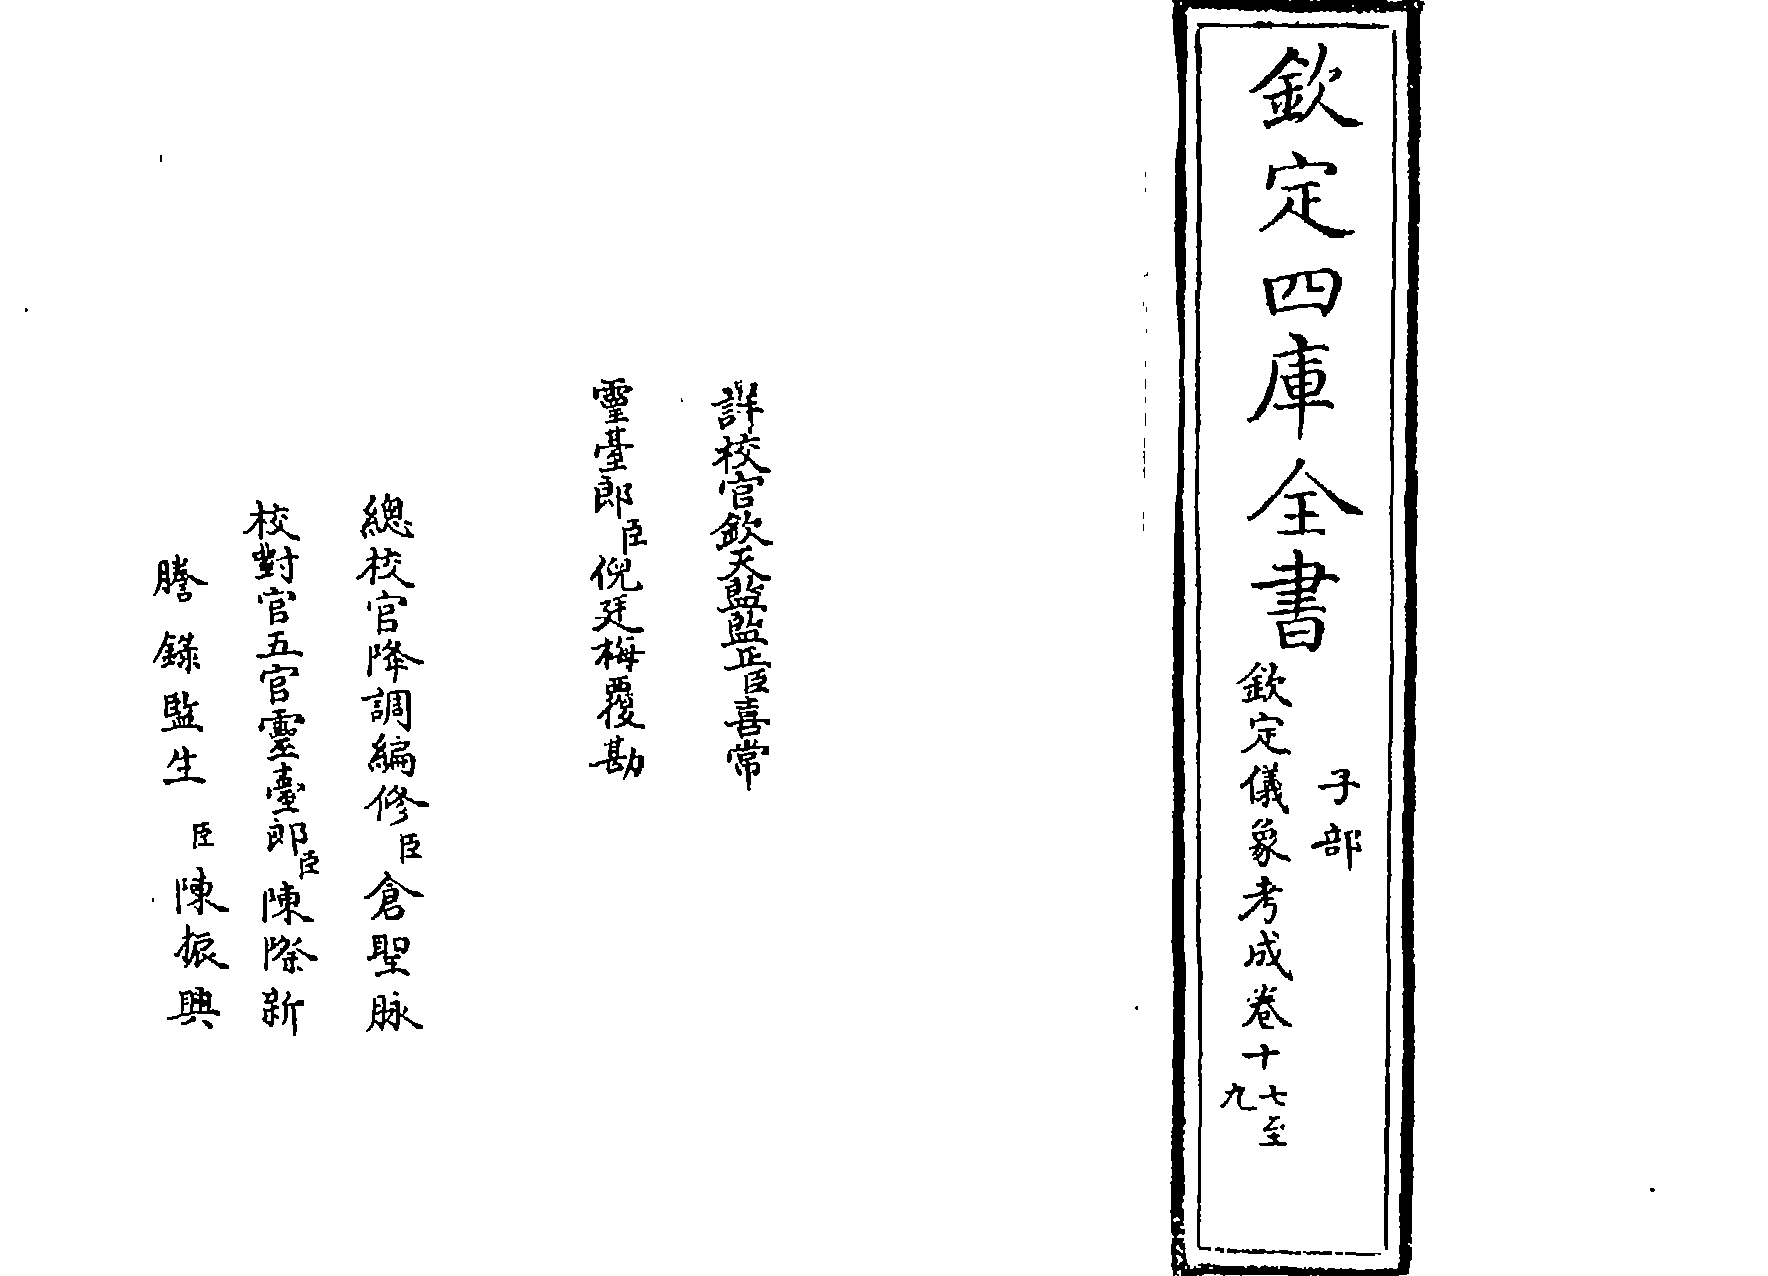
\includegraphics[width=\paperwidth,height=\paperheight,keepaspectratio]{img/1152.png}\clearpage
\begin{正文}
% ---- 册793 葉1153 ----
\SetPageNumber{1}
欽定四庫全書\换行
欽定儀象考成卷十七\换行
　恒星赤道經緯度表四\换行
　　赤道降婁宫\双列{\右小列{黄道度附}\左小列{}}\换行
\char"200B\relax\换行
\char"200B\relax\换行
\char"200B\relax\换行
\char"200B\relax\换行
\char"200B\relax\换行
\char"200B\relax\换行
\char"200B\relax\换行
\char"200B\relax\换行
\char"200B\relax\换行
\char"200B\relax\换行
\char"200B\relax\换行
\char"200B\relax
\par
\end{正文}\clearpage
\嵌图{146.67pt}{202.46pt}{838.42pt}{584.87pt}{img/1156.png}
\begin{正文}
% ---- 册793 葉1156 图版 ----
\SetPageNumber{2}
\插图页
\char"200B\relax\换行
\char"200B\relax\换行
\char"200B\relax\换行
\char"200B\relax\换行
\char"200B\relax\换行
\char"200B\relax\换行
\char"200B\relax\换行
\char"200B\relax\换行
\char"200B\relax\换行
\char"200B\relax\换行
\char"200B\relax\换行
\char"200B\relax\换行
\char"200B\relax\换行
\char"200B\relax\换行
\char"200B\relax\换行
\char"200B\relax
\恢复丝栏\par
\end{正文}\clearpage
\嵌图{148.67pt}{202.87pt}{834.42pt}{584.06pt}{img/1157.png}
\begin{正文}
% ---- 册793 葉1157 图版 ----
\SetPageNumber{3}
\插图页
\char"200B\relax\换行
\char"200B\relax\换行
\char"200B\relax\换行
\char"200B\relax\换行
\char"200B\relax\换行
\char"200B\relax\换行
\char"200B\relax\换行
\char"200B\relax\换行
\char"200B\relax\换行
\char"200B\relax\换行
\char"200B\relax\换行
\char"200B\relax\换行
\char"200B\relax\换行
\char"200B\relax\换行
\char"200B\relax\换行
\char"200B\relax
\恢复丝栏\par
\end{正文}\clearpage
\嵌图{142.64pt}{201.97pt}{846.47pt}{585.85pt}{img/1160.png}
\begin{正文}
% ---- 册793 葉1160 图版 ----
\SetPageNumber{4}
\插图页
\char"200B\relax\换行
\char"200B\relax\换行
\char"200B\relax\换行
\char"200B\relax\换行
\char"200B\relax\换行
\char"200B\relax\换行
\char"200B\relax\换行
\char"200B\relax\换行
\char"200B\relax\换行
\char"200B\relax\换行
\char"200B\relax\换行
\char"200B\relax\换行
\char"200B\relax\换行
\char"200B\relax\换行
\char"200B\relax\换行
\char"200B\relax
\恢复丝栏\par
\end{正文}\clearpage
\嵌图{146.62pt}{202.89pt}{838.53pt}{584.00pt}{img/1161.png}
\begin{正文}
% ---- 册793 葉1161 图版 ----
\SetPageNumber{5}
\插图页
\char"200B\relax\换行
\char"200B\relax\换行
\char"200B\relax\换行
\char"200B\relax\换行
\char"200B\relax\换行
\char"200B\relax\换行
\char"200B\relax\换行
\char"200B\relax\换行
\char"200B\relax\换行
\char"200B\relax\换行
\char"200B\relax\换行
\char"200B\relax\换行
\char"200B\relax\换行
\char"200B\relax\换行
\char"200B\relax\换行
\char"200B\relax
\恢复丝栏\par
\end{正文}\clearpage
\嵌图{144.63pt}{201.02pt}{842.50pt}{587.76pt}{img/1164.png}
\begin{正文}
% ---- 册793 葉1164 图版 ----
\SetPageNumber{6}
\插图页
\char"200B\relax\换行
\char"200B\relax\换行
\char"200B\relax\换行
\char"200B\relax\换行
\char"200B\relax\换行
\char"200B\relax\换行
\char"200B\relax\换行
\char"200B\relax\换行
\char"200B\relax\换行
\char"200B\relax\换行
\char"200B\relax\换行
\char"200B\relax\换行
\char"200B\relax\换行
\char"200B\relax\换行
\char"200B\relax\换行
\char"200B\relax
\恢复丝栏\par
\end{正文}\clearpage
\嵌图{146.62pt}{203.80pt}{838.53pt}{582.19pt}{img/1165.png}
\begin{正文}
% ---- 册793 葉1165 图版 ----
\SetPageNumber{7}
\插图页
\char"200B\relax\换行
\char"200B\relax\换行
\char"200B\relax\换行
\char"200B\relax\换行
\char"200B\relax\换行
\char"200B\relax\换行
\char"200B\relax\换行
\char"200B\relax\换行
\char"200B\relax\换行
\char"200B\relax\换行
\char"200B\relax\换行
\char"200B\relax\换行
\char"200B\relax\换行
\char"200B\relax\换行
\char"200B\relax\换行
\char"200B\relax
\恢复丝栏\par
\end{正文}\clearpage
\嵌图{140.71pt}{205.34pt}{850.34pt}{579.11pt}{img/1168.png}
\begin{正文}
% ---- 册793 葉1168 图版 ----
\SetPageNumber{8}
\插图页
\char"200B\relax\换行
\char"200B\relax\换行
\char"200B\relax\换行
\char"200B\relax\换行
\char"200B\relax\换行
\char"200B\relax\换行
\char"200B\relax\换行
\char"200B\relax\换行
\char"200B\relax\换行
\char"200B\relax\换行
\char"200B\relax\换行
\char"200B\relax\换行
\char"200B\relax\换行
\char"200B\relax\换行
\char"200B\relax\换行
\char"200B\relax
\恢复丝栏\par
\end{正文}\clearpage
\嵌图{142.72pt}{202.02pt}{846.33pt}{585.75pt}{img/1169.png}
\begin{正文}
% ---- 册793 葉1169 图版 ----
\SetPageNumber{9}
\插图页
\char"200B\relax\换行
\char"200B\relax\换行
\char"200B\relax\换行
\char"200B\relax\换行
\char"200B\relax\换行
\char"200B\relax\换行
\char"200B\relax\换行
\char"200B\relax\换行
\char"200B\relax\换行
\char"200B\relax\换行
\char"200B\relax\换行
\char"200B\relax\换行
\char"200B\relax\换行
\char"200B\relax\换行
\char"200B\relax\换行
\char"200B\relax
\恢复丝栏\par
\end{正文}\clearpage
\嵌图{144.63pt}{204.80pt}{842.50pt}{580.18pt}{img/1172.png}
\begin{正文}
% ---- 册793 葉1172 图版 ----
\SetPageNumber{10}
\插图页
\char"200B\relax\换行
\char"200B\relax\换行
\char"200B\relax\换行
\char"200B\relax\换行
\char"200B\relax\换行
\char"200B\relax\换行
\char"200B\relax\换行
\char"200B\relax\换行
\char"200B\relax\换行
\char"200B\relax\换行
\char"200B\relax\换行
\char"200B\relax\换行
\char"200B\relax\换行
\char"200B\relax\换行
\char"200B\relax\换行
\char"200B\relax
\恢复丝栏\par
\end{正文}\clearpage
\嵌图{146.62pt}{203.78pt}{838.53pt}{582.23pt}{img/1173.png}
\begin{正文}
% ---- 册793 葉1173 图版 ----
\SetPageNumber{11}
\插图页
\char"200B\relax\换行
\char"200B\relax\换行
\char"200B\relax\换行
\char"200B\relax\换行
\char"200B\relax\换行
\char"200B\relax\换行
\char"200B\relax\换行
\char"200B\relax\换行
\char"200B\relax\换行
\char"200B\relax\换行
\char"200B\relax\换行
\char"200B\relax\换行
\char"200B\relax\换行
\char"200B\relax\换行
\char"200B\relax\换行
\char"200B\relax
\恢复丝栏\par
\end{正文}\clearpage
\嵌图{140.68pt}{203.00pt}{850.39pt}{583.79pt}{img/1176.png}
\begin{正文}
% ---- 册793 葉1176 图版 ----
\SetPageNumber{12}
\插图页
\char"200B\relax\换行
\char"200B\relax\换行
\char"200B\relax\换行
\char"200B\relax\换行
\char"200B\relax\换行
\char"200B\relax\换行
\char"200B\relax\换行
\char"200B\relax\换行
\char"200B\relax\换行
\char"200B\relax\换行
\char"200B\relax\换行
\char"200B\relax\换行
\char"200B\relax\换行
\char"200B\relax\换行
\char"200B\relax\换行
\char"200B\relax
\恢复丝栏\par
\end{正文}\clearpage
\嵌图{142.68pt}{202.50pt}{846.40pt}{584.78pt}{img/1177.png}
\begin{正文}
% ---- 册793 葉1177 图版 ----
\SetPageNumber{13}
\插图页
\char"200B\relax\换行
\char"200B\relax\换行
\char"200B\relax\换行
\char"200B\relax\换行
\char"200B\relax\换行
\char"200B\relax\换行
\char"200B\relax\换行
\char"200B\relax\换行
\char"200B\relax\换行
\char"200B\relax\换行
\char"200B\relax\换行
\char"200B\relax\换行
\char"200B\relax\换行
\char"200B\relax\换行
\char"200B\relax\换行
\char"200B\relax
\恢复丝栏\par
\end{正文}\clearpage
\嵌图{144.68pt}{203.81pt}{842.41pt}{582.17pt}{img/1180.png}
\begin{正文}
% ---- 册793 葉1180 图版 ----
\SetPageNumber{14}
\插图页
\char"200B\relax\换行
\char"200B\relax\换行
\char"200B\relax\换行
\char"200B\relax\换行
\char"200B\relax\换行
\char"200B\relax\换行
\char"200B\relax\换行
\char"200B\relax\换行
\char"200B\relax\换行
\char"200B\relax\换行
\char"200B\relax\换行
\char"200B\relax\换行
\char"200B\relax\换行
\char"200B\relax\换行
\char"200B\relax\换行
\char"200B\relax
\恢复丝栏\par
\end{正文}\clearpage
\嵌图{144.68pt}{202.45pt}{842.41pt}{584.88pt}{img/1181.png}
\begin{正文}
% ---- 册793 葉1181 图版 ----
\SetPageNumber{15}
\插图页
\char"200B\relax\换行
\char"200B\relax\换行
\char"200B\relax\换行
\char"200B\relax\换行
\char"200B\relax\换行
\char"200B\relax\换行
\char"200B\relax\换行
\char"200B\relax\换行
\char"200B\relax\换行
\char"200B\relax\换行
\char"200B\relax\换行
\char"200B\relax\换行
\char"200B\relax\换行
\char"200B\relax\换行
\char"200B\relax\换行
\char"200B\relax
\恢复丝栏\par
\end{正文}\clearpage
\嵌图{140.66pt}{201.50pt}{850.45pt}{586.80pt}{img/1184.png}
\begin{正文}
% ---- 册793 葉1184 图版 ----
\SetPageNumber{16}
\插图页
\char"200B\relax\换行
\char"200B\relax\换行
\char"200B\relax\换行
\char"200B\relax\换行
\char"200B\relax\换行
\char"200B\relax\换行
\char"200B\relax\换行
\char"200B\relax\换行
\char"200B\relax\换行
\char"200B\relax\换行
\char"200B\relax\换行
\char"200B\relax\换行
\char"200B\relax\换行
\char"200B\relax\换行
\char"200B\relax\换行
\char"200B\relax
\恢复丝栏\par
\end{正文}\clearpage
\嵌图{142.64pt}{201.51pt}{846.47pt}{586.77pt}{img/1185.png}
\begin{正文}
% ---- 册793 葉1185 图版 ----
\SetPageNumber{17}
\插图页
\char"200B\relax\换行
\char"200B\relax\换行
\char"200B\relax\换行
\char"200B\relax\换行
\char"200B\relax\换行
\char"200B\relax\换行
\char"200B\relax\换行
\char"200B\relax\换行
\char"200B\relax\换行
\char"200B\relax\换行
\char"200B\relax\换行
\char"200B\relax\换行
\char"200B\relax\换行
\char"200B\relax\换行
\char"200B\relax\换行
\char"200B\relax
\恢复丝栏\par
\end{正文}\clearpage
\嵌图{146.67pt}{201.02pt}{838.42pt}{587.74pt}{img/1188.png}
\begin{正文}
% ---- 册793 葉1188 图版 ----
\SetPageNumber{18}
\插图页
\char"200B\relax\换行
\char"200B\relax\换行
\char"200B\relax\换行
\char"200B\relax\换行
\char"200B\relax\换行
\char"200B\relax\换行
\char"200B\relax\换行
\char"200B\relax\换行
\char"200B\relax\换行
\char"200B\relax\换行
\char"200B\relax\换行
\char"200B\relax\换行
\char"200B\relax\换行
\char"200B\relax\换行
\char"200B\relax\换行
\char"200B\relax
\恢复丝栏\par
\end{正文}\clearpage
\嵌图{146.67pt}{202.92pt}{838.42pt}{583.95pt}{img/1189.png}
\begin{正文}
% ---- 册793 葉1189 图版 ----
\SetPageNumber{19}
\插图页
\char"200B\relax\换行
\char"200B\relax\换行
\char"200B\relax\换行
\char"200B\relax\换行
\char"200B\relax\换行
\char"200B\relax\换行
\char"200B\relax\换行
\char"200B\relax\换行
\char"200B\relax\换行
\char"200B\relax\换行
\char"200B\relax\换行
\char"200B\relax\换行
\char"200B\relax\换行
\char"200B\relax\换行
\char"200B\relax\换行
\char"200B\relax
\恢复丝栏\par
\end{正文}\clearpage
\嵌图{150.30pt}{206.70pt}{831.15pt}{576.39pt}{img/1192.png}
\begin{正文}
% ---- 册793 葉1192 图版 ----
\SetPageNumber{20}
\插图页
\char"200B\relax\换行
\char"200B\relax\换行
\char"200B\relax\换行
\char"200B\relax\换行
\char"200B\relax\换行
\char"200B\relax\换行
\char"200B\relax\换行
\char"200B\relax\换行
\char"200B\relax\换行
\char"200B\relax\换行
\char"200B\relax\换行
\char"200B\relax\换行
\char"200B\relax\换行
\char"200B\relax\换行
\char"200B\relax\换行
\char"200B\relax
\恢复丝栏\par
\end{正文}\clearpage
\嵌图{193.20pt}{210.32pt}{543.58pt}{582.51pt}{img/1193.png}
\begin{正文}
% ---- 册793 葉1193 ----
\SetPageNumber{21}
\插图页
\char"200B\relax\换行
\char"200B\relax\换行
\char"200B\relax\换行
\char"200B\relax\换行
\char"200B\relax\换行
\char"200B\relax\换行
\char"200B\relax\换行
\char"200B\relax\换行
\恢复丝栏
\char"200B\relax\换行
\char"200B\relax\换行
\char"200B\relax\换行
\char"200B\relax\换行
\char"200B\relax\换行
\char"200B\relax\换行
\char"200B\relax\换行
欽定儀象考成卷十七
\par

% ======== 卷十八（8行21字）========
\par\end{正文}\clearpage
\chapter*{欽定儀象考成卷十八}
\begin{正文}
% ---- 册793 葉1196 ----
\SetPageNumber{1}
欽定四庫全書\换行
欽定儀象考成卷十八\换行
　恒星赤道經緯度表五\换行
　　赤道大梁宫\双列{\右小列{黄道度附}\左小列{}}\换行
\char"200B\relax\换行
\char"200B\relax\换行
\char"200B\relax\换行
\char"200B\relax\换行
\char"200B\relax\换行
\char"200B\relax\换行
\char"200B\relax\换行
\char"200B\relax\换行
\char"200B\relax\换行
\char"200B\relax\换行
\char"200B\relax\换行
\char"200B\relax
\par
\end{正文}\clearpage
\嵌图{144.63pt}{202.85pt}{842.50pt}{584.09pt}{img/1197.png}
\begin{正文}
% ---- 册793 葉1197 图版 ----
\SetPageNumber{2}
\插图页
\char"200B\relax\换行
\char"200B\relax\换行
\char"200B\relax\换行
\char"200B\relax\换行
\char"200B\relax\换行
\char"200B\relax\换行
\char"200B\relax\换行
\char"200B\relax\换行
\char"200B\relax\换行
\char"200B\relax\换行
\char"200B\relax\换行
\char"200B\relax\换行
\char"200B\relax\换行
\char"200B\relax\换行
\char"200B\relax\换行
\char"200B\relax
\恢复丝栏\par
\end{正文}\clearpage
\嵌图{142.68pt}{201.56pt}{846.40pt}{586.67pt}{img/1200.png}
\begin{正文}
% ---- 册793 葉1200 图版 ----
\SetPageNumber{3}
\插图页
\char"200B\relax\换行
\char"200B\relax\换行
\char"200B\relax\换行
\char"200B\relax\换行
\char"200B\relax\换行
\char"200B\relax\换行
\char"200B\relax\换行
\char"200B\relax\换行
\char"200B\relax\换行
\char"200B\relax\换行
\char"200B\relax\换行
\char"200B\relax\换行
\char"200B\relax\换行
\char"200B\relax\换行
\char"200B\relax\换行
\char"200B\relax
\恢复丝栏\par
\end{正文}\clearpage
\嵌图{142.68pt}{202.49pt}{846.40pt}{584.80pt}{img/1201.png}
\begin{正文}
% ---- 册793 葉1201 图版 ----
\SetPageNumber{4}
\插图页
\char"200B\relax\换行
\char"200B\relax\换行
\char"200B\relax\换行
\char"200B\relax\换行
\char"200B\relax\换行
\char"200B\relax\换行
\char"200B\relax\换行
\char"200B\relax\换行
\char"200B\relax\换行
\char"200B\relax\换行
\char"200B\relax\换行
\char"200B\relax\换行
\char"200B\relax\换行
\char"200B\relax\换行
\char"200B\relax\换行
\char"200B\relax
\恢复丝栏\par
\end{正文}\clearpage
\嵌图{146.62pt}{201.48pt}{838.53pt}{586.83pt}{img/1204.png}
\begin{正文}
% ---- 册793 葉1204 图版 ----
\SetPageNumber{5}
\插图页
\char"200B\relax\换行
\char"200B\relax\换行
\char"200B\relax\换行
\char"200B\relax\换行
\char"200B\relax\换行
\char"200B\relax\换行
\char"200B\relax\换行
\char"200B\relax\换行
\char"200B\relax\换行
\char"200B\relax\换行
\char"200B\relax\换行
\char"200B\relax\换行
\char"200B\relax\换行
\char"200B\relax\换行
\char"200B\relax\换行
\char"200B\relax
\恢复丝栏\par
\end{正文}\clearpage
\嵌图{146.62pt}{201.01pt}{838.53pt}{587.77pt}{img/1205.png}
\begin{正文}
% ---- 册793 葉1205 图版 ----
\SetPageNumber{6}
\插图页
\char"200B\relax\换行
\char"200B\relax\换行
\char"200B\relax\换行
\char"200B\relax\换行
\char"200B\relax\换行
\char"200B\relax\换行
\char"200B\relax\换行
\char"200B\relax\换行
\char"200B\relax\换行
\char"200B\relax\换行
\char"200B\relax\换行
\char"200B\relax\换行
\char"200B\relax\换行
\char"200B\relax\换行
\char"200B\relax\换行
\char"200B\relax
\恢复丝栏\par
\end{正文}\clearpage
\嵌图{144.68pt}{201.57pt}{842.41pt}{586.66pt}{img/1208.png}
\begin{正文}
% ---- 册793 葉1208 图版 ----
\SetPageNumber{7}
\插图页
\char"200B\relax\换行
\char"200B\relax\换行
\char"200B\relax\换行
\char"200B\relax\换行
\char"200B\relax\换行
\char"200B\relax\换行
\char"200B\relax\换行
\char"200B\relax\换行
\char"200B\relax\换行
\char"200B\relax\换行
\char"200B\relax\换行
\char"200B\relax\换行
\char"200B\relax\换行
\char"200B\relax\换行
\char"200B\relax\换行
\char"200B\relax
\恢复丝栏\par
\end{正文}\clearpage
\嵌图{142.68pt}{202.52pt}{846.40pt}{584.75pt}{img/1209.png}
\begin{正文}
% ---- 册793 葉1209 图版 ----
\SetPageNumber{8}
\插图页
\char"200B\relax\换行
\char"200B\relax\换行
\char"200B\relax\换行
\char"200B\relax\换行
\char"200B\relax\换行
\char"200B\relax\换行
\char"200B\relax\换行
\char"200B\relax\换行
\char"200B\relax\换行
\char"200B\relax\换行
\char"200B\relax\换行
\char"200B\relax\换行
\char"200B\relax\换行
\char"200B\relax\换行
\char"200B\relax\换行
\char"200B\relax
\恢复丝栏\par
\end{正文}\clearpage
\嵌图{146.67pt}{200.53pt}{838.42pt}{588.73pt}{img/1212.png}
\begin{正文}
% ---- 册793 葉1212 图版 ----
\SetPageNumber{9}
\插图页
\char"200B\relax\换行
\char"200B\relax\换行
\char"200B\relax\换行
\char"200B\relax\换行
\char"200B\relax\换行
\char"200B\relax\换行
\char"200B\relax\换行
\char"200B\relax\换行
\char"200B\relax\换行
\char"200B\relax\换行
\char"200B\relax\换行
\char"200B\relax\换行
\char"200B\relax\换行
\char"200B\relax\换行
\char"200B\relax\换行
\char"200B\relax
\恢复丝栏\par
\end{正文}\clearpage
\嵌图{146.67pt}{201.03pt}{838.42pt}{587.73pt}{img/1213.png}
\begin{正文}
% ---- 册793 葉1213 图版 ----
\SetPageNumber{10}
\插图页
\char"200B\relax\换行
\char"200B\relax\换行
\char"200B\relax\换行
\char"200B\relax\换行
\char"200B\relax\换行
\char"200B\relax\换行
\char"200B\relax\换行
\char"200B\relax\换行
\char"200B\relax\换行
\char"200B\relax\换行
\char"200B\relax\换行
\char"200B\relax\换行
\char"200B\relax\换行
\char"200B\relax\换行
\char"200B\relax\换行
\char"200B\relax
\恢复丝栏\par
\end{正文}\clearpage
\嵌图{148.61pt}{200.57pt}{834.55pt}{588.65pt}{img/1216.png}
\begin{正文}
% ---- 册793 葉1216 图版 ----
\SetPageNumber{11}
\插图页
\char"200B\relax\换行
\char"200B\relax\换行
\char"200B\relax\换行
\char"200B\relax\换行
\char"200B\relax\换行
\char"200B\relax\换行
\char"200B\relax\换行
\char"200B\relax\换行
\char"200B\relax\换行
\char"200B\relax\换行
\char"200B\relax\换行
\char"200B\relax\换行
\char"200B\relax\换行
\char"200B\relax\换行
\char"200B\relax\换行
\char"200B\relax
\恢复丝栏\par
\end{正文}\clearpage
\嵌图{144.63pt}{202.01pt}{842.50pt}{585.77pt}{img/1217.png}
\begin{正文}
% ---- 册793 葉1217 图版 ----
\SetPageNumber{12}
\插图页
\char"200B\relax\换行
\char"200B\relax\换行
\char"200B\relax\换行
\char"200B\relax\换行
\char"200B\relax\换行
\char"200B\relax\换行
\char"200B\relax\换行
\char"200B\relax\换行
\char"200B\relax\换行
\char"200B\relax\换行
\char"200B\relax\换行
\char"200B\relax\换行
\char"200B\relax\换行
\char"200B\relax\换行
\char"200B\relax\换行
\char"200B\relax
\恢复丝栏\par
\end{正文}\clearpage
\嵌图{146.62pt}{200.59pt}{838.53pt}{588.61pt}{img/1220.png}
\begin{正文}
% ---- 册793 葉1220 图版 ----
\SetPageNumber{13}
\插图页
\char"200B\relax\换行
\char"200B\relax\换行
\char"200B\relax\换行
\char"200B\relax\换行
\char"200B\relax\换行
\char"200B\relax\换行
\char"200B\relax\换行
\char"200B\relax\换行
\char"200B\relax\换行
\char"200B\relax\换行
\char"200B\relax\换行
\char"200B\relax\换行
\char"200B\relax\换行
\char"200B\relax\换行
\char"200B\relax\换行
\char"200B\relax
\恢复丝栏\par
\end{正文}\clearpage
\嵌图{144.63pt}{201.02pt}{842.50pt}{587.76pt}{img/1221.png}
\begin{正文}
% ---- 册793 葉1221 图版 ----
\SetPageNumber{14}
\插图页
\char"200B\relax\换行
\char"200B\relax\换行
\char"200B\relax\换行
\char"200B\relax\换行
\char"200B\relax\换行
\char"200B\relax\换行
\char"200B\relax\换行
\char"200B\relax\换行
\char"200B\relax\换行
\char"200B\relax\换行
\char"200B\relax\换行
\char"200B\relax\换行
\char"200B\relax\换行
\char"200B\relax\换行
\char"200B\relax\换行
\char"200B\relax
\恢复丝栏\par
\end{正文}\clearpage
\嵌图{146.56pt}{202.00pt}{838.64pt}{585.78pt}{img/1224.png}
\begin{正文}
% ---- 册793 葉1224 图版 ----
\SetPageNumber{15}
\插图页
\char"200B\relax\换行
\char"200B\relax\换行
\char"200B\relax\换行
\char"200B\relax\换行
\char"200B\relax\换行
\char"200B\relax\换行
\char"200B\relax\换行
\char"200B\relax\换行
\char"200B\relax\换行
\char"200B\relax\换行
\char"200B\relax\换行
\char"200B\relax\换行
\char"200B\relax\换行
\char"200B\relax\换行
\char"200B\relax\换行
\char"200B\relax
\恢复丝栏\par
\end{正文}\clearpage
\嵌图{148.54pt}{200.55pt}{834.68pt}{588.69pt}{img/1225.png}
\begin{正文}
% ---- 册793 葉1225 图版 ----
\SetPageNumber{16}
\插图页
\char"200B\relax\换行
\char"200B\relax\换行
\char"200B\relax\换行
\char"200B\relax\换行
\char"200B\relax\换行
\char"200B\relax\换行
\char"200B\relax\换行
\char"200B\relax\换行
\char"200B\relax\换行
\char"200B\relax\换行
\char"200B\relax\换行
\char"200B\relax\换行
\char"200B\relax\换行
\char"200B\relax\换行
\char"200B\relax\换行
\char"200B\relax
\恢复丝栏\par
\end{正文}\clearpage
\嵌图{146.56pt}{202.93pt}{838.64pt}{583.94pt}{img/1228.png}
\begin{正文}
% ---- 册793 葉1228 图版 ----
\SetPageNumber{17}
\插图页
\char"200B\relax\换行
\char"200B\relax\换行
\char"200B\relax\换行
\char"200B\relax\换行
\char"200B\relax\换行
\char"200B\relax\换行
\char"200B\relax\换行
\char"200B\relax\换行
\char"200B\relax\换行
\char"200B\relax\换行
\char"200B\relax\换行
\char"200B\relax\换行
\char"200B\relax\换行
\char"200B\relax\换行
\char"200B\relax\换行
\char"200B\relax
\恢复丝栏\par
\end{正文}\clearpage
\嵌图{148.54pt}{200.49pt}{834.68pt}{588.80pt}{img/1229.png}
\begin{正文}
% ---- 册793 葉1229 图版 ----
\SetPageNumber{18}
\插图页
\char"200B\relax\换行
\char"200B\relax\换行
\char"200B\relax\换行
\char"200B\relax\换行
\char"200B\relax\换行
\char"200B\relax\换行
\char"200B\relax\换行
\char"200B\relax\换行
\char"200B\relax\换行
\char"200B\relax\换行
\char"200B\relax\换行
\char"200B\relax\换行
\char"200B\relax\换行
\char"200B\relax\换行
\char"200B\relax\换行
\char"200B\relax
\恢复丝栏\par
\end{正文}\clearpage
\嵌图{154.21pt}{201.07pt}{823.35pt}{587.64pt}{img/1232.png}
\begin{正文}
% ---- 册793 葉1232 图版 ----
\SetPageNumber{19}
\插图页
\char"200B\relax\换行
\char"200B\relax\换行
\char"200B\relax\换行
\char"200B\relax\换行
\char"200B\relax\换行
\char"200B\relax\换行
\char"200B\relax\换行
\char"200B\relax\换行
\char"200B\relax\换行
\char"200B\relax\换行
\char"200B\relax\换行
\char"200B\relax\换行
\char"200B\relax\换行
\char"200B\relax\换行
\char"200B\relax\换行
\char"200B\relax
\恢复丝栏\par
\end{正文}\clearpage
\嵌图{170.46pt}{235.03pt}{173.48pt}{586.18pt}{img/1233.png}
\begin{正文}
% ---- 册793 葉1233 ----
\SetPageNumber{20}
\char"200B\relax\换行
\char"200B\relax\换行
\char"200B\relax\换行
\char"200B\relax\换行
\char"200B\relax\换行
\char"200B\relax\换行
\char"200B\relax\换行
\char"200B\relax\换行
\char"200B\relax\换行
\char"200B\relax\换行
\char"200B\relax\换行
\char"200B\relax\换行
\char"200B\relax\换行
\char"200B\relax\换行
\char"200B\relax\换行
欽定儀象考成卷十八
\par

% ======== 卷十九（8行21字）========
\par\end{正文}\clearpage
\chapter*{欽定儀象考成卷十九}
\begin{正文}
% ---- 册793 葉1236 ----
\SetPageNumber{1}
欽定四庫全書\换行
欽定儀象考成卷十九\换行
　恒星赤道經緯度表六\换行
　　赤道實沈宫\双列{\右小列{黄道度附}\左小列{}}\换行
\char"200B\relax\换行
\char"200B\relax\换行
\char"200B\relax\换行
\char"200B\relax\换行
\char"200B\relax\换行
\char"200B\relax\换行
\char"200B\relax\换行
\char"200B\relax\换行
\char"200B\relax\换行
\char"200B\relax\换行
\char"200B\relax\换行
\char"200B\relax
\par
\end{正文}\clearpage
\嵌图{146.56pt}{200.07pt}{838.64pt}{589.65pt}{img/1237.png}
\begin{正文}
% ---- 册793 葉1237 图版 ----
\SetPageNumber{2}
\插图页
\char"200B\relax\换行
\char"200B\relax\换行
\char"200B\relax\换行
\char"200B\relax\换行
\char"200B\relax\换行
\char"200B\relax\换行
\char"200B\relax\换行
\char"200B\relax\换行
\char"200B\relax\换行
\char"200B\relax\换行
\char"200B\relax\换行
\char"200B\relax\换行
\char"200B\relax\换行
\char"200B\relax\换行
\char"200B\relax\换行
\char"200B\relax
\恢复丝栏\par
\end{正文}\clearpage
\嵌图{144.63pt}{202.03pt}{842.50pt}{585.74pt}{img/1240.png}
\begin{正文}
% ---- 册793 葉1240 图版 ----
\SetPageNumber{3}
\插图页
\char"200B\relax\换行
\char"200B\relax\换行
\char"200B\relax\换行
\char"200B\relax\换行
\char"200B\relax\换行
\char"200B\relax\换行
\char"200B\relax\换行
\char"200B\relax\换行
\char"200B\relax\换行
\char"200B\relax\换行
\char"200B\relax\换行
\char"200B\relax\换行
\char"200B\relax\换行
\char"200B\relax\换行
\char"200B\relax\换行
\char"200B\relax
\恢复丝栏\par
\end{正文}\clearpage
\嵌图{144.63pt}{200.59pt}{842.50pt}{588.61pt}{img/1241.png}
\begin{正文}
% ---- 册793 葉1241 图版 ----
\SetPageNumber{4}
\插图页
\char"200B\relax\换行
\char"200B\relax\换行
\char"200B\relax\换行
\char"200B\relax\换行
\char"200B\relax\换行
\char"200B\relax\换行
\char"200B\relax\换行
\char"200B\relax\换行
\char"200B\relax\换行
\char"200B\relax\换行
\char"200B\relax\换行
\char"200B\relax\换行
\char"200B\relax\换行
\char"200B\relax\换行
\char"200B\relax\换行
\char"200B\relax
\恢复丝栏\par
\end{正文}\clearpage
\嵌图{144.68pt}{201.56pt}{842.41pt}{586.67pt}{img/1244.png}
\begin{正文}
% ---- 册793 葉1244 图版 ----
\SetPageNumber{5}
\插图页
\char"200B\relax\换行
\char"200B\relax\换行
\char"200B\relax\换行
\char"200B\relax\换行
\char"200B\relax\换行
\char"200B\relax\换行
\char"200B\relax\换行
\char"200B\relax\换行
\char"200B\relax\换行
\char"200B\relax\换行
\char"200B\relax\换行
\char"200B\relax\换行
\char"200B\relax\换行
\char"200B\relax\换行
\char"200B\relax\换行
\char"200B\relax
\恢复丝栏\par
\end{正文}\clearpage
\嵌图{142.68pt}{202.90pt}{846.40pt}{583.99pt}{img/1245.png}
\begin{正文}
% ---- 册793 葉1245 图版 ----
\SetPageNumber{6}
\插图页
\char"200B\relax\换行
\char"200B\relax\换行
\char"200B\relax\换行
\char"200B\relax\换行
\char"200B\relax\换行
\char"200B\relax\换行
\char"200B\relax\换行
\char"200B\relax\换行
\char"200B\relax\换行
\char"200B\relax\换行
\char"200B\relax\换行
\char"200B\relax\换行
\char"200B\relax\换行
\char"200B\relax\换行
\char"200B\relax\换行
\char"200B\relax
\恢复丝栏\par
\end{正文}\clearpage
\嵌图{142.64pt}{203.00pt}{846.47pt}{583.79pt}{img/1248.png}
\begin{正文}
% ---- 册793 葉1248 图版 ----
\SetPageNumber{7}
\插图页
\char"200B\relax\换行
\char"200B\relax\换行
\char"200B\relax\换行
\char"200B\relax\换行
\char"200B\relax\换行
\char"200B\relax\换行
\char"200B\relax\换行
\char"200B\relax\换行
\char"200B\relax\换行
\char"200B\relax\换行
\char"200B\relax\换行
\char"200B\relax\换行
\char"200B\relax\换行
\char"200B\relax\换行
\char"200B\relax\换行
\char"200B\relax
\恢复丝栏\par
\end{正文}\clearpage
\嵌图{146.62pt}{200.59pt}{838.53pt}{588.61pt}{img/1249.png}
\begin{正文}
% ---- 册793 葉1249 图版 ----
\SetPageNumber{8}
\插图页
\char"200B\relax\换行
\char"200B\relax\换行
\char"200B\relax\换行
\char"200B\relax\换行
\char"200B\relax\换行
\char"200B\relax\换行
\char"200B\relax\换行
\char"200B\relax\换行
\char"200B\relax\换行
\char"200B\relax\换行
\char"200B\relax\换行
\char"200B\relax\换行
\char"200B\relax\换行
\char"200B\relax\换行
\char"200B\relax\换行
\char"200B\relax
\恢复丝栏\par
\end{正文}\clearpage
\嵌图{146.62pt}{201.56pt}{838.53pt}{586.67pt}{img/1252.png}
\begin{正文}
% ---- 册793 葉1252 图版 ----
\SetPageNumber{9}
\插图页
\char"200B\relax\换行
\char"200B\relax\换行
\char"200B\relax\换行
\char"200B\relax\换行
\char"200B\relax\换行
\char"200B\relax\换行
\char"200B\relax\换行
\char"200B\relax\换行
\char"200B\relax\换行
\char"200B\relax\换行
\char"200B\relax\换行
\char"200B\relax\换行
\char"200B\relax\换行
\char"200B\relax\换行
\char"200B\relax\换行
\char"200B\relax
\恢复丝栏\par
\end{正文}\clearpage
\嵌图{144.63pt}{201.99pt}{842.50pt}{585.80pt}{img/1253.png}
\begin{正文}
% ---- 册793 葉1253 图版 ----
\SetPageNumber{10}
\插图页
\char"200B\relax\换行
\char"200B\relax\换行
\char"200B\relax\换行
\char"200B\relax\换行
\char"200B\relax\换行
\char"200B\relax\换行
\char"200B\relax\换行
\char"200B\relax\换行
\char"200B\relax\换行
\char"200B\relax\换行
\char"200B\relax\换行
\char"200B\relax\换行
\char"200B\relax\换行
\char"200B\relax\换行
\char"200B\relax\换行
\char"200B\relax
\恢复丝栏\par
\end{正文}\clearpage
\嵌图{144.59pt}{204.41pt}{842.59pt}{580.97pt}{img/1256.png}
\begin{正文}
% ---- 册793 葉1256 图版 ----
\SetPageNumber{11}
\插图页
\char"200B\relax\换行
\char"200B\relax\换行
\char"200B\relax\换行
\char"200B\relax\换行
\char"200B\relax\换行
\char"200B\relax\换行
\char"200B\relax\换行
\char"200B\relax\换行
\char"200B\relax\换行
\char"200B\relax\换行
\char"200B\relax\换行
\char"200B\relax\换行
\char"200B\relax\换行
\char"200B\relax\换行
\char"200B\relax\换行
\char"200B\relax
\恢复丝栏\par
\end{正文}\clearpage
\嵌图{142.61pt}{202.95pt}{846.55pt}{583.88pt}{img/1257.png}
\begin{正文}
% ---- 册793 葉1257 图版 ----
\SetPageNumber{12}
\插图页
\char"200B\relax\换行
\char"200B\relax\换行
\char"200B\relax\换行
\char"200B\relax\换行
\char"200B\relax\换行
\char"200B\relax\换行
\char"200B\relax\换行
\char"200B\relax\换行
\char"200B\relax\换行
\char"200B\relax\换行
\char"200B\relax\换行
\char"200B\relax\换行
\char"200B\relax\换行
\char"200B\relax\换行
\char"200B\relax\换行
\char"200B\relax
\恢复丝栏\par
\end{正文}\clearpage
\嵌图{146.62pt}{202.89pt}{838.53pt}{584.00pt}{img/1260.png}
\begin{正文}
% ---- 册793 葉1260 图版 ----
\SetPageNumber{13}
\插图页
\char"200B\relax\换行
\char"200B\relax\换行
\char"200B\relax\换行
\char"200B\relax\换行
\char"200B\relax\换行
\char"200B\relax\换行
\char"200B\relax\换行
\char"200B\relax\换行
\char"200B\relax\换行
\char"200B\relax\换行
\char"200B\relax\换行
\char"200B\relax\换行
\char"200B\relax\换行
\char"200B\relax\换行
\char"200B\relax\换行
\char"200B\relax
\恢复丝栏\par
\end{正文}\clearpage
\嵌图{142.64pt}{200.99pt}{846.47pt}{587.82pt}{img/1261.png}
\begin{正文}
% ---- 册793 葉1261 图版 ----
\SetPageNumber{14}
\插图页
\char"200B\relax\换行
\char"200B\relax\换行
\char"200B\relax\换行
\char"200B\relax\换行
\char"200B\relax\换行
\char"200B\relax\换行
\char"200B\relax\换行
\char"200B\relax\换行
\char"200B\relax\换行
\char"200B\relax\换行
\char"200B\relax\换行
\char"200B\relax\换行
\char"200B\relax\换行
\char"200B\relax\换行
\char"200B\relax\换行
\char"200B\relax
\恢复丝栏\par
\end{正文}\clearpage
\嵌图{144.63pt}{202.02pt}{842.50pt}{585.75pt}{img/1264.png}
\begin{正文}
% ---- 册793 葉1264 图版 ----
\SetPageNumber{15}
\插图页
\char"200B\relax\换行
\char"200B\relax\换行
\char"200B\relax\换行
\char"200B\relax\换行
\char"200B\relax\换行
\char"200B\relax\换行
\char"200B\relax\换行
\char"200B\relax\换行
\char"200B\relax\换行
\char"200B\relax\换行
\char"200B\relax\换行
\char"200B\relax\换行
\char"200B\relax\换行
\char"200B\relax\换行
\char"200B\relax\换行
\char"200B\relax
\恢复丝栏\par
\end{正文}\clearpage
\嵌图{142.64pt}{200.11pt}{846.47pt}{589.56pt}{img/1265.png}
\begin{正文}
% ---- 册793 葉1265 图版 ----
\SetPageNumber{16}
\插图页
\char"200B\relax\换行
\char"200B\relax\换行
\char"200B\relax\换行
\char"200B\relax\换行
\char"200B\relax\换行
\char"200B\relax\换行
\char"200B\relax\换行
\char"200B\relax\换行
\char"200B\relax\换行
\char"200B\relax\换行
\char"200B\relax\换行
\char"200B\relax\换行
\char"200B\relax\换行
\char"200B\relax\换行
\char"200B\relax\换行
\char"200B\relax
\恢复丝栏\par
\end{正文}\clearpage
\嵌图{144.59pt}{202.46pt}{842.59pt}{584.87pt}{img/1268.png}
\begin{正文}
% ---- 册793 葉1268 图版 ----
\SetPageNumber{17}
\插图页
\char"200B\relax\换行
\char"200B\relax\换行
\char"200B\relax\换行
\char"200B\relax\换行
\char"200B\relax\换行
\char"200B\relax\换行
\char"200B\relax\换行
\char"200B\relax\换行
\char"200B\relax\换行
\char"200B\relax\换行
\char"200B\relax\换行
\char"200B\relax\换行
\char"200B\relax\换行
\char"200B\relax\换行
\char"200B\relax\换行
\char"200B\relax
\恢复丝栏\par
\end{正文}\clearpage
\嵌图{144.59pt}{202.42pt}{842.59pt}{584.95pt}{img/1269.png}
\begin{正文}
% ---- 册793 葉1269 图版 ----
\SetPageNumber{18}
\插图页
\char"200B\relax\换行
\char"200B\relax\换行
\char"200B\relax\换行
\char"200B\relax\换行
\char"200B\relax\换行
\char"200B\relax\换行
\char"200B\relax\换行
\char"200B\relax\换行
\char"200B\relax\换行
\char"200B\relax\换行
\char"200B\relax\换行
\char"200B\relax\换行
\char"200B\relax\换行
\char"200B\relax\换行
\char"200B\relax\换行
\char"200B\relax
\恢复丝栏\par
\end{正文}\clearpage
\嵌图{148.61pt}{199.14pt}{834.55pt}{591.51pt}{img/1272.png}
\begin{正文}
% ---- 册793 葉1272 图版 ----
\SetPageNumber{19}
\插图页
\char"200B\relax\换行
\char"200B\relax\换行
\char"200B\relax\换行
\char"200B\relax\换行
\char"200B\relax\换行
\char"200B\relax\换行
\char"200B\relax\换行
\char"200B\relax\换行
\char"200B\relax\换行
\char"200B\relax\换行
\char"200B\relax\换行
\char"200B\relax\换行
\char"200B\relax\换行
\char"200B\relax\换行
\char"200B\relax\换行
\char"200B\relax
\恢复丝栏\par
\end{正文}\clearpage
\嵌图{146.62pt}{199.59pt}{838.53pt}{590.60pt}{img/1273.png}
\begin{正文}
% ---- 册793 葉1273 图版 ----
\SetPageNumber{20}
\插图页
\char"200B\relax\换行
\char"200B\relax\换行
\char"200B\relax\换行
\char"200B\relax\换行
\char"200B\relax\换行
\char"200B\relax\换行
\char"200B\relax\换行
\char"200B\relax\换行
\char"200B\relax\换行
\char"200B\relax\换行
\char"200B\relax\换行
\char"200B\relax\换行
\char"200B\relax\换行
\char"200B\relax\换行
\char"200B\relax\换行
\char"200B\relax
\恢复丝栏\par
\end{正文}\clearpage
\嵌图{144.68pt}{202.50pt}{842.41pt}{584.78pt}{img/1276.png}
\begin{正文}
% ---- 册793 葉1276 图版 ----
\SetPageNumber{21}
\插图页
\char"200B\relax\换行
\char"200B\relax\换行
\char"200B\relax\换行
\char"200B\relax\换行
\char"200B\relax\换行
\char"200B\relax\换行
\char"200B\relax\换行
\char"200B\relax\换行
\char"200B\relax\换行
\char"200B\relax\换行
\char"200B\relax\换行
\char"200B\relax\换行
\char"200B\relax\换行
\char"200B\relax\换行
\char"200B\relax\换行
\char"200B\relax
\恢复丝栏\par
\end{正文}\clearpage
\嵌图{146.67pt}{201.04pt}{838.42pt}{587.72pt}{img/1277.png}
\begin{正文}
% ---- 册793 葉1277 图版 ----
\SetPageNumber{22}
\插图页
\char"200B\relax\换行
\char"200B\relax\换行
\char"200B\relax\换行
\char"200B\relax\换行
\char"200B\relax\换行
\char"200B\relax\换行
\char"200B\relax\换行
\char"200B\relax\换行
\char"200B\relax\换行
\char"200B\relax\换行
\char"200B\relax\换行
\char"200B\relax\换行
\char"200B\relax\换行
\char"200B\relax\换行
\char"200B\relax\换行
\char"200B\relax
\恢复丝栏\par
\end{正文}\clearpage
\嵌图{148.42pt}{200.55pt}{834.93pt}{588.69pt}{img/1280.png}
\begin{正文}
% ---- 册793 葉1280 图版 ----
\SetPageNumber{23}
\插图页
\char"200B\relax\换行
\char"200B\relax\换行
\char"200B\relax\换行
\char"200B\relax\换行
\char"200B\relax\换行
\char"200B\relax\换行
\char"200B\relax\换行
\char"200B\relax\换行
\char"200B\relax\换行
\char"200B\relax\换行
\char"200B\relax\换行
\char"200B\relax\换行
\char"200B\relax\换行
\char"200B\relax\换行
\char"200B\relax\换行
\char"200B\relax
\恢复丝栏\par
\end{正文}\clearpage
\嵌图{141.38pt}{220.50pt}{406.64pt}{572.33pt}{img/1281.png}
\begin{正文}
% ---- 册793 葉1281 ----
\SetPageNumber{24}
\插图页
\char"200B\relax\换行
\char"200B\relax\换行
\char"200B\relax\换行
\char"200B\relax\换行
\char"200B\relax\换行
\char"200B\relax\换行
\char"200B\relax\换行
\char"200B\relax\换行
\恢复丝栏
\char"200B\relax\换行
\char"200B\relax\换行
\char"200B\relax\换行
\char"200B\relax\换行
\char"200B\relax\换行
\char"200B\relax\换行
\char"200B\relax\换行
欽定儀象考成卷十九
\par

% ======== 卷二十（8行21字）========
\par\end{正文}\clearpage
\chapter*{欽定儀象考成卷二十}
\begin{正文}
\end{正文}\clearpage

  \thispagestyle{empty}\noindent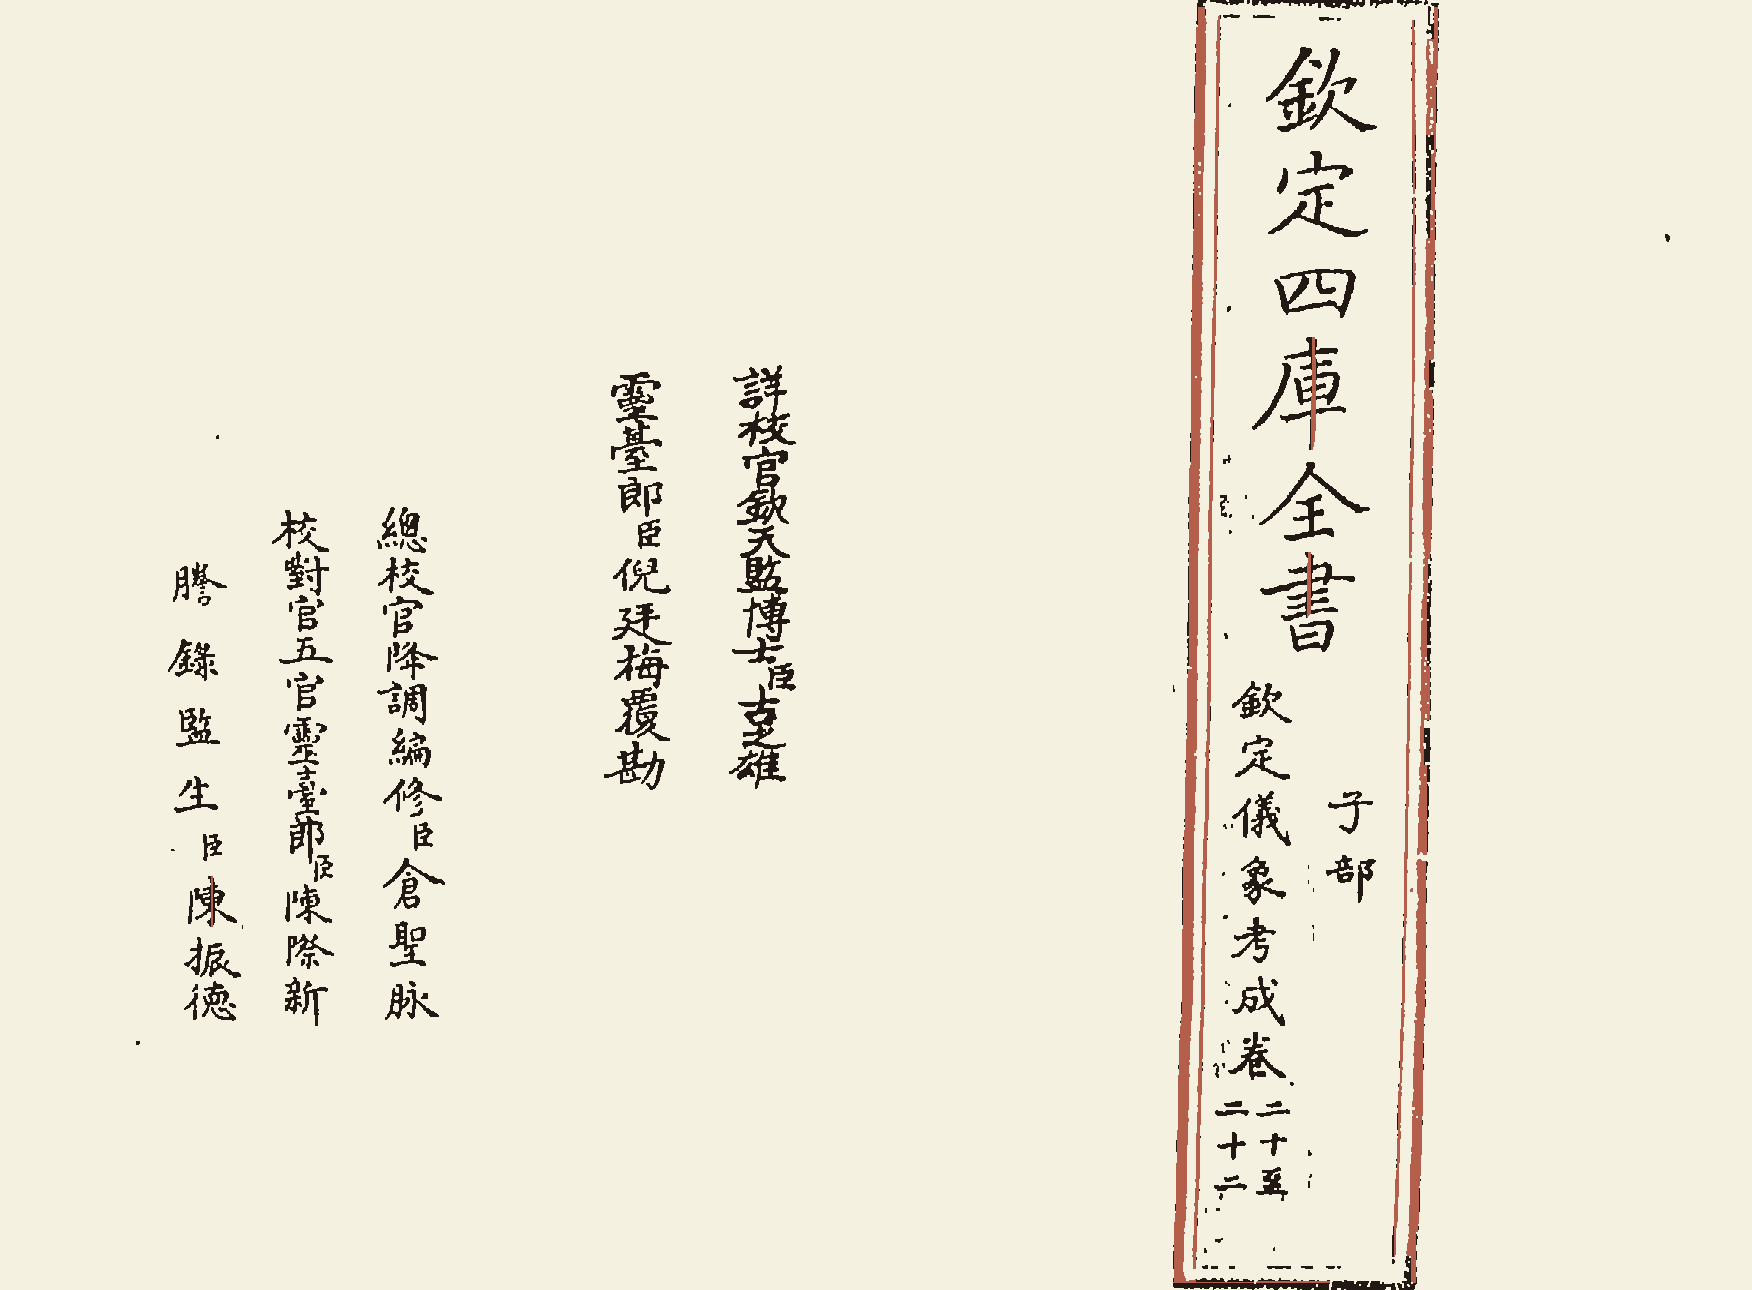
\includegraphics[width=\paperwidth,height=\paperheight,keepaspectratio]{img/1284.png}\clearpage
\begin{正文}
% ---- 册793 葉1285 ----
\SetPageNumber{1}
欽定四庫全書\换行
欽定儀象考成卷二十\换行
　恒星赤道經緯度表七\换行
　　赤道鶉首宫\双列{\右小列{黄道度附}\左小列{}}\换行
\char"200B\relax\换行
\char"200B\relax\换行
\char"200B\relax\换行
\char"200B\relax\换行
\char"200B\relax\换行
\char"200B\relax\换行
\char"200B\relax\换行
\char"200B\relax\换行
\char"200B\relax\换行
\char"200B\relax\换行
\char"200B\relax\换行
\char"200B\relax
\par
\end{正文}\clearpage
\嵌图{142.57pt}{201.98pt}{846.62pt}{585.83pt}{img/1288.png}
\begin{正文}
% ---- 册793 葉1288 图版 ----
\SetPageNumber{2}
\插图页
\char"200B\relax\换行
\char"200B\relax\换行
\char"200B\relax\换行
\char"200B\relax\换行
\char"200B\relax\换行
\char"200B\relax\换行
\char"200B\relax\换行
\char"200B\relax\换行
\char"200B\relax\换行
\char"200B\relax\换行
\char"200B\relax\换行
\char"200B\relax\换行
\char"200B\relax\换行
\char"200B\relax\换行
\char"200B\relax\换行
\char"200B\relax
\恢复丝栏\par
\end{正文}\clearpage
\嵌图{144.54pt}{203.37pt}{842.68pt}{583.06pt}{img/1289.png}
\begin{正文}
% ---- 册793 葉1289 图版 ----
\SetPageNumber{3}
\插图页
\char"200B\relax\换行
\char"200B\relax\换行
\char"200B\relax\换行
\char"200B\relax\换行
\char"200B\relax\换行
\char"200B\relax\换行
\char"200B\relax\换行
\char"200B\relax\换行
\char"200B\relax\换行
\char"200B\relax\换行
\char"200B\relax\换行
\char"200B\relax\换行
\char"200B\relax\换行
\char"200B\relax\换行
\char"200B\relax\换行
\char"200B\relax
\恢复丝栏\par
\end{正文}\clearpage
\嵌图{140.66pt}{206.04pt}{850.45pt}{577.72pt}{img/1292.png}
\begin{正文}
% ---- 册793 葉1292 图版 ----
\SetPageNumber{4}
\插图页
\char"200B\relax\换行
\char"200B\relax\换行
\char"200B\relax\换行
\char"200B\relax\换行
\char"200B\relax\换行
\char"200B\relax\换行
\char"200B\relax\换行
\char"200B\relax\换行
\char"200B\relax\换行
\char"200B\relax\换行
\char"200B\relax\换行
\char"200B\relax\换行
\char"200B\relax\换行
\char"200B\relax\换行
\char"200B\relax\换行
\char"200B\relax
\恢复丝栏\par
\end{正文}\clearpage
\嵌图{142.64pt}{200.46pt}{846.47pt}{588.87pt}{img/1293.png}
\begin{正文}
% ---- 册793 葉1293 图版 ----
\SetPageNumber{5}
\插图页
\char"200B\relax\换行
\char"200B\relax\换行
\char"200B\relax\换行
\char"200B\relax\换行
\char"200B\relax\换行
\char"200B\relax\换行
\char"200B\relax\换行
\char"200B\relax\换行
\char"200B\relax\换行
\char"200B\relax\换行
\char"200B\relax\换行
\char"200B\relax\换行
\char"200B\relax\换行
\char"200B\relax\换行
\char"200B\relax\换行
\char"200B\relax
\恢复丝栏\par
\end{正文}\clearpage
\嵌图{144.72pt}{198.69pt}{842.31pt}{592.42pt}{img/1296.png}
\begin{正文}
% ---- 册793 葉1296 图版 ----
\SetPageNumber{6}
\插图页
\char"200B\relax\换行
\char"200B\relax\换行
\char"200B\relax\换行
\char"200B\relax\换行
\char"200B\relax\换行
\char"200B\relax\换行
\char"200B\relax\换行
\char"200B\relax\换行
\char"200B\relax\换行
\char"200B\relax\换行
\char"200B\relax\换行
\char"200B\relax\换行
\char"200B\relax\换行
\char"200B\relax\换行
\char"200B\relax\换行
\char"200B\relax
\恢复丝栏\par
\end{正文}\clearpage
\嵌图{146.73pt}{198.18pt}{838.30pt}{593.43pt}{img/1297.png}
\begin{正文}
% ---- 册793 葉1297 图版 ----
\SetPageNumber{7}
\插图页
\char"200B\relax\换行
\char"200B\relax\换行
\char"200B\relax\换行
\char"200B\relax\换行
\char"200B\relax\换行
\char"200B\relax\换行
\char"200B\relax\换行
\char"200B\relax\换行
\char"200B\relax\换行
\char"200B\relax\换行
\char"200B\relax\换行
\char"200B\relax\换行
\char"200B\relax\换行
\char"200B\relax\换行
\char"200B\relax\换行
\char"200B\relax
\恢复丝栏\par
\end{正文}\clearpage
\嵌图{144.63pt}{202.87pt}{842.50pt}{584.06pt}{img/1300.png}
\begin{正文}
% ---- 册793 葉1300 图版 ----
\SetPageNumber{8}
\插图页
\char"200B\relax\换行
\char"200B\relax\换行
\char"200B\relax\换行
\char"200B\relax\换行
\char"200B\relax\换行
\char"200B\relax\换行
\char"200B\relax\换行
\char"200B\relax\换行
\char"200B\relax\换行
\char"200B\relax\换行
\char"200B\relax\换行
\char"200B\relax\换行
\char"200B\relax\换行
\char"200B\relax\换行
\char"200B\relax\换行
\char"200B\relax
\恢复丝栏\par
\end{正文}\clearpage
\嵌图{146.62pt}{202.82pt}{838.53pt}{584.14pt}{img/1301.png}
\begin{正文}
% ---- 册793 葉1301 图版 ----
\SetPageNumber{9}
\插图页
\char"200B\relax\换行
\char"200B\relax\换行
\char"200B\relax\换行
\char"200B\relax\换行
\char"200B\relax\换行
\char"200B\relax\换行
\char"200B\relax\换行
\char"200B\relax\换行
\char"200B\relax\换行
\char"200B\relax\换行
\char"200B\relax\换行
\char"200B\relax\换行
\char"200B\relax\换行
\char"200B\relax\换行
\char"200B\relax\换行
\char"200B\relax
\恢复丝栏\par
\end{正文}\clearpage
\嵌图{142.72pt}{199.59pt}{846.33pt}{590.60pt}{img/1304.png}
\begin{正文}
% ---- 册793 葉1304 图版 ----
\SetPageNumber{10}
\插图页
\char"200B\relax\换行
\char"200B\relax\换行
\char"200B\relax\换行
\char"200B\relax\换行
\char"200B\relax\换行
\char"200B\relax\换行
\char"200B\relax\换行
\char"200B\relax\换行
\char"200B\relax\换行
\char"200B\relax\换行
\char"200B\relax\换行
\char"200B\relax\换行
\char"200B\relax\换行
\char"200B\relax\换行
\char"200B\relax\换行
\char"200B\relax
\恢复丝栏\par
\end{正文}\clearpage
\嵌图{144.72pt}{200.99pt}{842.31pt}{587.80pt}{img/1305.png}
\begin{正文}
% ---- 册793 葉1305 图版 ----
\SetPageNumber{11}
\插图页
\char"200B\relax\换行
\char"200B\relax\换行
\char"200B\relax\换行
\char"200B\relax\换行
\char"200B\relax\换行
\char"200B\relax\换行
\char"200B\relax\换行
\char"200B\relax\换行
\char"200B\relax\换行
\char"200B\relax\换行
\char"200B\relax\换行
\char"200B\relax\换行
\char"200B\relax\换行
\char"200B\relax\换行
\char"200B\relax\换行
\char"200B\relax
\恢复丝栏\par
\end{正文}\clearpage
\嵌图{144.72pt}{200.06pt}{842.31pt}{589.68pt}{img/1308.png}
\begin{正文}
% ---- 册793 葉1308 图版 ----
\SetPageNumber{12}
\插图页
\char"200B\relax\换行
\char"200B\relax\换行
\char"200B\relax\换行
\char"200B\relax\换行
\char"200B\relax\换行
\char"200B\relax\换行
\char"200B\relax\换行
\char"200B\relax\换行
\char"200B\relax\换行
\char"200B\relax\换行
\char"200B\relax\换行
\char"200B\relax\换行
\char"200B\relax\换行
\char"200B\relax\换行
\char"200B\relax\换行
\char"200B\relax
\恢复丝栏\par
\end{正文}\clearpage
\嵌图{146.73pt}{199.08pt}{838.30pt}{591.64pt}{img/1309.png}
\begin{正文}
% ---- 册793 葉1309 图版 ----
\SetPageNumber{13}
\插图页
\char"200B\relax\换行
\char"200B\relax\换行
\char"200B\relax\换行
\char"200B\relax\换行
\char"200B\relax\换行
\char"200B\relax\换行
\char"200B\relax\换行
\char"200B\relax\换行
\char"200B\relax\换行
\char"200B\relax\换行
\char"200B\relax\换行
\char"200B\relax\换行
\char"200B\relax\换行
\char"200B\relax\换行
\char"200B\relax\换行
\char"200B\relax
\恢复丝栏\par
\end{正文}\clearpage
\嵌图{142.68pt}{201.95pt}{846.40pt}{585.88pt}{img/1312.png}
\begin{正文}
% ---- 册793 葉1312 图版 ----
\SetPageNumber{14}
\插图页
\char"200B\relax\换行
\char"200B\relax\换行
\char"200B\relax\换行
\char"200B\relax\换行
\char"200B\relax\换行
\char"200B\relax\换行
\char"200B\relax\换行
\char"200B\relax\换行
\char"200B\relax\换行
\char"200B\relax\换行
\char"200B\relax\换行
\char"200B\relax\换行
\char"200B\relax\换行
\char"200B\relax\换行
\char"200B\relax\换行
\char"200B\relax
\恢复丝栏\par
\end{正文}\clearpage
\嵌图{144.68pt}{199.56pt}{842.41pt}{590.66pt}{img/1313.png}
\begin{正文}
% ---- 册793 葉1313 图版 ----
\SetPageNumber{15}
\插图页
\char"200B\relax\换行
\char"200B\relax\换行
\char"200B\relax\换行
\char"200B\relax\换行
\char"200B\relax\换行
\char"200B\relax\换行
\char"200B\relax\换行
\char"200B\relax\换行
\char"200B\relax\换行
\char"200B\relax\换行
\char"200B\relax\换行
\char"200B\relax\换行
\char"200B\relax\换行
\char"200B\relax\换行
\char"200B\relax\换行
\char"200B\relax
\恢复丝栏\par
\end{正文}\clearpage
\嵌图{146.67pt}{201.49pt}{838.42pt}{586.81pt}{img/1316.png}
\begin{正文}
% ---- 册793 葉1316 图版 ----
\SetPageNumber{16}
\插图页
\char"200B\relax\换行
\char"200B\relax\换行
\char"200B\relax\换行
\char"200B\relax\换行
\char"200B\relax\换行
\char"200B\relax\换行
\char"200B\relax\换行
\char"200B\relax\换行
\char"200B\relax\换行
\char"200B\relax\换行
\char"200B\relax\换行
\char"200B\relax\换行
\char"200B\relax\换行
\char"200B\relax\换行
\char"200B\relax\换行
\char"200B\relax
\恢复丝栏\par
\end{正文}\clearpage
\嵌图{146.67pt}{198.64pt}{838.42pt}{592.51pt}{img/1317.png}
\begin{正文}
% ---- 册793 葉1317 图版 ----
\SetPageNumber{17}
\插图页
\char"200B\relax\换行
\char"200B\relax\换行
\char"200B\relax\换行
\char"200B\relax\换行
\char"200B\relax\换行
\char"200B\relax\换行
\char"200B\relax\换行
\char"200B\relax\换行
\char"200B\relax\换行
\char"200B\relax\换行
\char"200B\relax\换行
\char"200B\relax\换行
\char"200B\relax\换行
\char"200B\relax\换行
\char"200B\relax\换行
\char"200B\relax
\恢复丝栏\par
\end{正文}\clearpage
\嵌图{142.64pt}{201.01pt}{846.47pt}{587.77pt}{img/1320.png}
\begin{正文}
% ---- 册793 葉1320 图版 ----
\SetPageNumber{18}
\插图页
\char"200B\relax\换行
\char"200B\relax\换行
\char"200B\relax\换行
\char"200B\relax\换行
\char"200B\relax\换行
\char"200B\relax\换行
\char"200B\relax\换行
\char"200B\relax\换行
\char"200B\relax\换行
\char"200B\relax\换行
\char"200B\relax\换行
\char"200B\relax\换行
\char"200B\relax\换行
\char"200B\relax\换行
\char"200B\relax\换行
\char"200B\relax
\恢复丝栏\par
\end{正文}\clearpage
\嵌图{144.63pt}{202.91pt}{842.50pt}{583.97pt}{img/1321.png}
\begin{正文}
% ---- 册793 葉1321 图版 ----
\SetPageNumber{19}
\插图页
\char"200B\relax\换行
\char"200B\relax\换行
\char"200B\relax\换行
\char"200B\relax\换行
\char"200B\relax\换行
\char"200B\relax\换行
\char"200B\relax\换行
\char"200B\relax\换行
\char"200B\relax\换行
\char"200B\relax\换行
\char"200B\relax\换行
\char"200B\relax\换行
\char"200B\relax\换行
\char"200B\relax\换行
\char"200B\relax\换行
\char"200B\relax
\恢复丝栏\par
\end{正文}\clearpage
\嵌图{167.51pt}{236.84pt}{227.46pt}{584.37pt}{img/1324.png}
\begin{正文}
% ---- 册793 葉1324 ----
\SetPageNumber{20}
\char"200B\relax\换行
\char"200B\relax\换行
\char"200B\relax\换行
\char"200B\relax\换行
\char"200B\relax\换行
\char"200B\relax\换行
\char"200B\relax\换行
\char"200B\relax\换行
\char"200B\relax\换行
\char"200B\relax\换行
\char"200B\relax\换行
\char"200B\relax\换行
\char"200B\relax\换行
\char"200B\relax\换行
\char"200B\relax\换行
欽定儀象考成卷二十
\par

% ======== 卷二十一（8行21字）========
\par\end{正文}\clearpage
\chapter*{欽定儀象考成卷二十一}
\begin{正文}
% ---- 册793 葉1325 ----
\SetPageNumber{1}
欽定四庫全書\换行
欽定儀象考成卷二十一\换行
　恒星赤道經緯度表八\换行
　　赤道鶉火宫\双列{\右小列{黄道度附}\左小列{}}\换行
\char"200B\relax\换行
\char"200B\relax\换行
\char"200B\relax\换行
\char"200B\relax\换行
\char"200B\relax\换行
\char"200B\relax\换行
\char"200B\relax\换行
\char"200B\relax\换行
\char"200B\relax\换行
\char"200B\relax\换行
\char"200B\relax\换行
\char"200B\relax
\par
\end{正文}\clearpage
\嵌图{140.71pt}{198.20pt}{850.34pt}{593.39pt}{img/1328.png}
\begin{正文}
% ---- 册793 葉1328 图版 ----
\SetPageNumber{2}
\插图页
\char"200B\relax\换行
\char"200B\relax\换行
\char"200B\relax\换行
\char"200B\relax\换行
\char"200B\relax\换行
\char"200B\relax\换行
\char"200B\relax\换行
\char"200B\relax\换行
\char"200B\relax\换行
\char"200B\relax\换行
\char"200B\relax\换行
\char"200B\relax\换行
\char"200B\relax\换行
\char"200B\relax\换行
\char"200B\relax\换行
\char"200B\relax
\恢复丝栏\par
\end{正文}\clearpage
\嵌图{144.72pt}{199.15pt}{842.31pt}{591.49pt}{img/1329.png}
\begin{正文}
% ---- 册793 葉1329 图版 ----
\SetPageNumber{3}
\插图页
\char"200B\relax\换行
\char"200B\relax\换行
\char"200B\relax\换行
\char"200B\relax\换行
\char"200B\relax\换行
\char"200B\relax\换行
\char"200B\relax\换行
\char"200B\relax\换行
\char"200B\relax\换行
\char"200B\relax\换行
\char"200B\relax\换行
\char"200B\relax\换行
\char"200B\relax\换行
\char"200B\relax\换行
\char"200B\relax\换行
\char"200B\relax
\恢复丝栏\par
\end{正文}\clearpage
\嵌图{144.68pt}{201.47pt}{842.41pt}{586.86pt}{img/1332.png}
\begin{正文}
% ---- 册793 葉1332 图版 ----
\SetPageNumber{4}
\插图页
\char"200B\relax\换行
\char"200B\relax\换行
\char"200B\relax\换行
\char"200B\relax\换行
\char"200B\relax\换行
\char"200B\relax\换行
\char"200B\relax\换行
\char"200B\relax\换行
\char"200B\relax\换行
\char"200B\relax\换行
\char"200B\relax\换行
\char"200B\relax\换行
\char"200B\relax\换行
\char"200B\relax\换行
\char"200B\relax\换行
\char"200B\relax
\恢复丝栏\par
\end{正文}\clearpage
\嵌图{144.68pt}{200.51pt}{842.41pt}{588.77pt}{img/1333.png}
\begin{正文}
% ---- 册793 葉1333 图版 ----
\SetPageNumber{5}
\插图页
\char"200B\relax\换行
\char"200B\relax\换行
\char"200B\relax\换行
\char"200B\relax\换行
\char"200B\relax\换行
\char"200B\relax\换行
\char"200B\relax\换行
\char"200B\relax\换行
\char"200B\relax\换行
\char"200B\relax\换行
\char"200B\relax\换行
\char"200B\relax\换行
\char"200B\relax\换行
\char"200B\relax\换行
\char"200B\relax\换行
\char"200B\relax
\恢复丝栏\par
\end{正文}\clearpage
\嵌图{144.72pt}{200.61pt}{842.31pt}{588.57pt}{img/1336.png}
\begin{正文}
% ---- 册793 葉1336 图版 ----
\SetPageNumber{6}
\插图页
\char"200B\relax\换行
\char"200B\relax\换行
\char"200B\relax\换行
\char"200B\relax\换行
\char"200B\relax\换行
\char"200B\relax\换行
\char"200B\relax\换行
\char"200B\relax\换行
\char"200B\relax\换行
\char"200B\relax\换行
\char"200B\relax\换行
\char"200B\relax\换行
\char"200B\relax\换行
\char"200B\relax\换行
\char"200B\relax\换行
\char"200B\relax
\恢复丝栏\par
\end{正文}\clearpage
\嵌图{142.72pt}{198.19pt}{846.33pt}{593.41pt}{img/1337.png}
\begin{正文}
% ---- 册793 葉1337 图版 ----
\SetPageNumber{7}
\插图页
\char"200B\relax\换行
\char"200B\relax\换行
\char"200B\relax\换行
\char"200B\relax\换行
\char"200B\relax\换行
\char"200B\relax\换行
\char"200B\relax\换行
\char"200B\relax\换行
\char"200B\relax\换行
\char"200B\relax\换行
\char"200B\relax\换行
\char"200B\relax\换行
\char"200B\relax\换行
\char"200B\relax\换行
\char"200B\relax\换行
\char"200B\relax
\恢复丝栏\par
\end{正文}\clearpage
\嵌图{146.62pt}{200.58pt}{838.53pt}{588.64pt}{img/1340.png}
\begin{正文}
% ---- 册793 葉1340 图版 ----
\SetPageNumber{8}
\插图页
\char"200B\relax\换行
\char"200B\relax\换行
\char"200B\relax\换行
\char"200B\relax\换行
\char"200B\relax\换行
\char"200B\relax\换行
\char"200B\relax\换行
\char"200B\relax\换行
\char"200B\relax\换行
\char"200B\relax\换行
\char"200B\relax\换行
\char"200B\relax\换行
\char"200B\relax\换行
\char"200B\relax\换行
\char"200B\relax\换行
\char"200B\relax
\恢复丝栏\par
\end{正文}\clearpage
\嵌图{144.63pt}{199.12pt}{842.50pt}{591.55pt}{img/1341.png}
\begin{正文}
% ---- 册793 葉1341 图版 ----
\SetPageNumber{9}
\插图页
\char"200B\relax\换行
\char"200B\relax\换行
\char"200B\relax\换行
\char"200B\relax\换行
\char"200B\relax\换行
\char"200B\relax\换行
\char"200B\relax\换行
\char"200B\relax\换行
\char"200B\relax\换行
\char"200B\relax\换行
\char"200B\relax\换行
\char"200B\relax\换行
\char"200B\relax\换行
\char"200B\relax\换行
\char"200B\relax\换行
\char"200B\relax
\恢复丝栏\par
\end{正文}\clearpage
\嵌图{142.64pt}{200.11pt}{846.47pt}{589.58pt}{img/1344.png}
\begin{正文}
% ---- 册793 葉1344 图版 ----
\SetPageNumber{10}
\插图页
\char"200B\relax\换行
\char"200B\relax\换行
\char"200B\relax\换行
\char"200B\relax\换行
\char"200B\relax\换行
\char"200B\relax\换行
\char"200B\relax\换行
\char"200B\relax\换行
\char"200B\relax\换行
\char"200B\relax\换行
\char"200B\relax\换行
\char"200B\relax\换行
\char"200B\relax\换行
\char"200B\relax\换行
\char"200B\relax\换行
\char"200B\relax
\恢复丝栏\par
\end{正文}\clearpage
\嵌图{146.62pt}{198.67pt}{838.53pt}{592.45pt}{img/1345.png}
\begin{正文}
% ---- 册793 葉1345 图版 ----
\SetPageNumber{11}
\插图页
\char"200B\relax\换行
\char"200B\relax\换行
\char"200B\relax\换行
\char"200B\relax\换行
\char"200B\relax\换行
\char"200B\relax\换行
\char"200B\relax\换行
\char"200B\relax\换行
\char"200B\relax\换行
\char"200B\relax\换行
\char"200B\relax\换行
\char"200B\relax\换行
\char"200B\relax\换行
\char"200B\relax\换行
\char"200B\relax\换行
\char"200B\relax
\恢复丝栏\par
\end{正文}\clearpage
\嵌图{146.62pt}{202.94pt}{838.53pt}{583.90pt}{img/1348.png}
\begin{正文}
% ---- 册793 葉1348 图版 ----
\SetPageNumber{12}
\插图页
\char"200B\relax\换行
\char"200B\relax\换行
\char"200B\relax\换行
\char"200B\relax\换行
\char"200B\relax\换行
\char"200B\relax\换行
\char"200B\relax\换行
\char"200B\relax\换行
\char"200B\relax\换行
\char"200B\relax\换行
\char"200B\relax\换行
\char"200B\relax\换行
\char"200B\relax\换行
\char"200B\relax\换行
\char"200B\relax\换行
\char"200B\relax
\恢复丝栏\par
\end{正文}\clearpage
\嵌图{146.62pt}{201.02pt}{838.53pt}{587.76pt}{img/1349.png}
\begin{正文}
% ---- 册793 葉1349 图版 ----
\SetPageNumber{13}
\插图页
\char"200B\relax\换行
\char"200B\relax\换行
\char"200B\relax\换行
\char"200B\relax\换行
\char"200B\relax\换行
\char"200B\relax\换行
\char"200B\relax\换行
\char"200B\relax\换行
\char"200B\relax\换行
\char"200B\relax\换行
\char"200B\relax\换行
\char"200B\relax\换行
\char"200B\relax\换行
\char"200B\relax\换行
\char"200B\relax\换行
\char"200B\relax
\恢复丝栏\par
\end{正文}\clearpage
\嵌图{140.66pt}{202.49pt}{850.45pt}{584.80pt}{img/1352.png}
\begin{正文}
% ---- 册793 葉1352 图版 ----
\SetPageNumber{14}
\插图页
\char"200B\relax\换行
\char"200B\relax\换行
\char"200B\relax\换行
\char"200B\relax\换行
\char"200B\relax\换行
\char"200B\relax\换行
\char"200B\relax\换行
\char"200B\relax\换行
\char"200B\relax\换行
\char"200B\relax\换行
\char"200B\relax\换行
\char"200B\relax\换行
\char"200B\relax\换行
\char"200B\relax\换行
\char"200B\relax\换行
\char"200B\relax
\恢复丝栏\par
\end{正文}\clearpage
\嵌图{142.64pt}{200.08pt}{846.47pt}{589.63pt}{img/1353.png}
\begin{正文}
% ---- 册793 葉1353 图版 ----
\SetPageNumber{15}
\插图页
\char"200B\relax\换行
\char"200B\relax\换行
\char"200B\relax\换行
\char"200B\relax\换行
\char"200B\relax\换行
\char"200B\relax\换行
\char"200B\relax\换行
\char"200B\relax\换行
\char"200B\relax\换行
\char"200B\relax\换行
\char"200B\relax\换行
\char"200B\relax\换行
\char"200B\relax\换行
\char"200B\relax\换行
\char"200B\relax\换行
\char"200B\relax
\恢复丝栏\par
\end{正文}\clearpage
\嵌图{140.66pt}{201.00pt}{850.45pt}{587.79pt}{img/1356.png}
\begin{正文}
% ---- 册793 葉1356 图版 ----
\SetPageNumber{16}
\插图页
\char"200B\relax\换行
\char"200B\relax\换行
\char"200B\relax\换行
\char"200B\relax\换行
\char"200B\relax\换行
\char"200B\relax\换行
\char"200B\relax\换行
\char"200B\relax\换行
\char"200B\relax\换行
\char"200B\relax\换行
\char"200B\relax\换行
\char"200B\relax\换行
\char"200B\relax\换行
\char"200B\relax\换行
\char"200B\relax\换行
\char"200B\relax
\恢复丝栏\par
\end{正文}\clearpage
\嵌图{142.64pt}{201.88pt}{846.47pt}{586.02pt}{img/1357.png}
\begin{正文}
% ---- 册793 葉1357 图版 ----
\SetPageNumber{17}
\插图页
\char"200B\relax\换行
\char"200B\relax\换行
\char"200B\relax\换行
\char"200B\relax\换行
\char"200B\relax\换行
\char"200B\relax\换行
\char"200B\relax\换行
\char"200B\relax\换行
\char"200B\relax\换行
\char"200B\relax\换行
\char"200B\relax\换行
\char"200B\relax\换行
\char"200B\relax\换行
\char"200B\relax\换行
\char"200B\relax\换行
\char"200B\relax
\恢复丝栏\par
\end{正文}\clearpage
\嵌图{144.63pt}{199.13pt}{842.50pt}{591.52pt}{img/1360.png}
\begin{正文}
% ---- 册793 葉1360 图版 ----
\SetPageNumber{18}
\插图页
\char"200B\relax\换行
\char"200B\relax\换行
\char"200B\relax\换行
\char"200B\relax\换行
\char"200B\relax\换行
\char"200B\relax\换行
\char"200B\relax\换行
\char"200B\relax\换行
\char"200B\relax\换行
\char"200B\relax\换行
\char"200B\relax\换行
\char"200B\relax\换行
\char"200B\relax\换行
\char"200B\relax\换行
\char"200B\relax\换行
\char"200B\relax
\恢复丝栏\par
\end{正文}\clearpage
\嵌图{142.64pt}{200.57pt}{846.47pt}{588.65pt}{img/1361.png}
\begin{正文}
% ---- 册793 葉1361 图版 ----
\SetPageNumber{19}
\插图页
\char"200B\relax\换行
\char"200B\relax\换行
\char"200B\relax\换行
\char"200B\relax\换行
\char"200B\relax\换行
\char"200B\relax\换行
\char"200B\relax\换行
\char"200B\relax\换行
\char"200B\relax\换行
\char"200B\relax\换行
\char"200B\relax\换行
\char"200B\relax\换行
\char"200B\relax\换行
\char"200B\relax\换行
\char"200B\relax\换行
\char"200B\relax
\恢复丝栏\par
\end{正文}\clearpage
\嵌图{144.63pt}{200.99pt}{842.50pt}{587.82pt}{img/1364.png}
\begin{正文}
% ---- 册793 葉1364 图版 ----
\SetPageNumber{20}
\插图页
\char"200B\relax\换行
\char"200B\relax\换行
\char"200B\relax\换行
\char"200B\relax\换行
\char"200B\relax\换行
\char"200B\relax\换行
\char"200B\relax\换行
\char"200B\relax\换行
\char"200B\relax\换行
\char"200B\relax\换行
\char"200B\relax\换行
\char"200B\relax\换行
\char"200B\relax\换行
\char"200B\relax\换行
\char"200B\relax\换行
\char"200B\relax
\恢复丝栏\par
\end{正文}\clearpage
\嵌图{144.63pt}{199.08pt}{842.50pt}{591.64pt}{img/1365.png}
\begin{正文}
% ---- 册793 葉1365 图版 ----
\SetPageNumber{21}
\插图页
\char"200B\relax\换行
\char"200B\relax\换行
\char"200B\relax\换行
\char"200B\relax\换行
\char"200B\relax\换行
\char"200B\relax\换行
\char"200B\relax\换行
\char"200B\relax\换行
\char"200B\relax\换行
\char"200B\relax\换行
\char"200B\relax\换行
\char"200B\relax\换行
\char"200B\relax\换行
\char"200B\relax\换行
\char"200B\relax\换行
\char"200B\relax
\恢复丝栏\par
\end{正文}\clearpage
\嵌图{174.32pt}{212.19pt}{169.63pt}{580.64pt}{img/1368.png}
\begin{正文}
% ---- 册793 葉1368 ----
\SetPageNumber{22}
\char"200B\relax\换行
\char"200B\relax\换行
\char"200B\relax\换行
\char"200B\relax\换行
\char"200B\relax\换行
\char"200B\relax\换行
\char"200B\relax\换行
\char"200B\relax\换行
\char"200B\relax\换行
\char"200B\relax\换行
\char"200B\relax\换行
\char"200B\relax\换行
\char"200B\relax\换行
\char"200B\relax\换行
\char"200B\relax\换行
欽定儀象考成卷二十一
\par

% ======== 卷二十二（8行21字）========
\par\end{正文}\clearpage
\chapter*{欽定儀象考成卷二十二}
\begin{正文}
% ---- 册793 葉1369 ----
\SetPageNumber{1}
欽定四庫全書\换行
欽定儀象考成卷二十二\换行
　恒星赤道經緯度表九\换行
　　赤道鶉尾宫\双列{\右小列{黄道度附}\左小列{}}\换行
\char"200B\relax\换行
\char"200B\relax\换行
\char"200B\relax\换行
\char"200B\relax\换行
\char"200B\relax\换行
\char"200B\relax\换行
\char"200B\relax\换行
\char"200B\relax\换行
\char"200B\relax\换行
\char"200B\relax\换行
\char"200B\relax\换行
\char"200B\relax
\par
\end{正文}\clearpage
\嵌图{144.63pt}{198.62pt}{842.50pt}{592.56pt}{img/1372.png}
\begin{正文}
% ---- 册793 葉1372 图版 ----
\SetPageNumber{2}
\插图页
\char"200B\relax\换行
\char"200B\relax\换行
\char"200B\relax\换行
\char"200B\relax\换行
\char"200B\relax\换行
\char"200B\relax\换行
\char"200B\relax\换行
\char"200B\relax\换行
\char"200B\relax\换行
\char"200B\relax\换行
\char"200B\relax\换行
\char"200B\relax\换行
\char"200B\relax\换行
\char"200B\relax\换行
\char"200B\relax\换行
\char"200B\relax
\恢复丝栏\par
\end{正文}\clearpage
\嵌图{144.63pt}{200.97pt}{842.50pt}{587.86pt}{img/1373.png}
\begin{正文}
% ---- 册793 葉1373 图版 ----
\SetPageNumber{3}
\插图页
\char"200B\relax\换行
\char"200B\relax\换行
\char"200B\relax\换行
\char"200B\relax\换行
\char"200B\relax\换行
\char"200B\relax\换行
\char"200B\relax\换行
\char"200B\relax\换行
\char"200B\relax\换行
\char"200B\relax\换行
\char"200B\relax\换行
\char"200B\relax\换行
\char"200B\relax\换行
\char"200B\relax\换行
\char"200B\relax\换行
\char"200B\relax
\恢复丝栏\par
\end{正文}\clearpage
\嵌图{142.64pt}{199.65pt}{846.47pt}{590.49pt}{img/1376.png}
\begin{正文}
% ---- 册793 葉1376 图版 ----
\SetPageNumber{4}
\插图页
\char"200B\relax\换行
\char"200B\relax\换行
\char"200B\relax\换行
\char"200B\relax\换行
\char"200B\relax\换行
\char"200B\relax\换行
\char"200B\relax\换行
\char"200B\relax\换行
\char"200B\relax\换行
\char"200B\relax\换行
\char"200B\relax\换行
\char"200B\relax\换行
\char"200B\relax\换行
\char"200B\relax\换行
\char"200B\relax\换行
\char"200B\relax
\恢复丝栏\par
\end{正文}\clearpage
\嵌图{142.64pt}{200.56pt}{846.47pt}{588.68pt}{img/1377.png}
\begin{正文}
% ---- 册793 葉1377 图版 ----
\SetPageNumber{5}
\插图页
\char"200B\relax\换行
\char"200B\relax\换行
\char"200B\relax\换行
\char"200B\relax\换行
\char"200B\relax\换行
\char"200B\relax\换行
\char"200B\relax\换行
\char"200B\relax\换行
\char"200B\relax\换行
\char"200B\relax\换行
\char"200B\relax\换行
\char"200B\relax\换行
\char"200B\relax\换行
\char"200B\relax\换行
\char"200B\relax\换行
\char"200B\relax
\恢复丝栏\par
\end{正文}\clearpage
\嵌图{146.62pt}{201.07pt}{838.53pt}{587.66pt}{img/1380.png}
\begin{正文}
% ---- 册793 葉1380 图版 ----
\SetPageNumber{6}
\插图页
\char"200B\relax\换行
\char"200B\relax\换行
\char"200B\relax\换行
\char"200B\relax\换行
\char"200B\relax\换行
\char"200B\relax\换行
\char"200B\relax\换行
\char"200B\relax\换行
\char"200B\relax\换行
\char"200B\relax\换行
\char"200B\relax\换行
\char"200B\relax\换行
\char"200B\relax\换行
\char"200B\relax\换行
\char"200B\relax\换行
\char"200B\relax
\恢复丝栏\par
\end{正文}\clearpage
\嵌图{144.63pt}{199.13pt}{842.50pt}{591.54pt}{img/1381.png}
\begin{正文}
% ---- 册793 葉1381 图版 ----
\SetPageNumber{7}
\插图页
\char"200B\relax\换行
\char"200B\relax\换行
\char"200B\relax\换行
\char"200B\relax\换行
\char"200B\relax\换行
\char"200B\relax\换行
\char"200B\relax\换行
\char"200B\relax\换行
\char"200B\relax\换行
\char"200B\relax\换行
\char"200B\relax\换行
\char"200B\relax\换行
\char"200B\relax\换行
\char"200B\relax\换行
\char"200B\relax\换行
\char"200B\relax
\恢复丝栏\par
\end{正文}\clearpage
\嵌图{146.56pt}{202.88pt}{838.64pt}{584.02pt}{img/1384.png}
\begin{正文}
% ---- 册793 葉1384 图版 ----
\SetPageNumber{8}
\插图页
\char"200B\relax\换行
\char"200B\relax\换行
\char"200B\relax\换行
\char"200B\relax\换行
\char"200B\relax\换行
\char"200B\relax\换行
\char"200B\relax\换行
\char"200B\relax\换行
\char"200B\relax\换行
\char"200B\relax\换行
\char"200B\relax\换行
\char"200B\relax\换行
\char"200B\relax\换行
\char"200B\relax\换行
\char"200B\relax\换行
\char"200B\relax
\恢复丝栏\par
\end{正文}\clearpage
\嵌图{146.56pt}{202.40pt}{838.64pt}{584.98pt}{img/1385.png}
\begin{正文}
% ---- 册793 葉1385 图版 ----
\SetPageNumber{9}
\插图页
\char"200B\relax\换行
\char"200B\relax\换行
\char"200B\relax\换行
\char"200B\relax\换行
\char"200B\relax\换行
\char"200B\relax\换行
\char"200B\relax\换行
\char"200B\relax\换行
\char"200B\relax\换行
\char"200B\relax\换行
\char"200B\relax\换行
\char"200B\relax\换行
\char"200B\relax\换行
\char"200B\relax\换行
\char"200B\relax\换行
\char"200B\relax
\恢复丝栏\par
\end{正文}\clearpage
\嵌图{148.54pt}{201.96pt}{834.68pt}{585.86pt}{img/1388.png}
\begin{正文}
% ---- 册793 葉1388 图版 ----
\SetPageNumber{10}
\插图页
\char"200B\relax\换行
\char"200B\relax\换行
\char"200B\relax\换行
\char"200B\relax\换行
\char"200B\relax\换行
\char"200B\relax\换行
\char"200B\relax\换行
\char"200B\relax\换行
\char"200B\relax\换行
\char"200B\relax\换行
\char"200B\relax\换行
\char"200B\relax\换行
\char"200B\relax\换行
\char"200B\relax\换行
\char"200B\relax\换行
\char"200B\relax
\恢复丝栏\par
\end{正文}\clearpage
\嵌图{144.59pt}{199.08pt}{842.59pt}{591.63pt}{img/1389.png}
\begin{正文}
% ---- 册793 葉1389 图版 ----
\SetPageNumber{11}
\插图页
\char"200B\relax\换行
\char"200B\relax\换行
\char"200B\relax\换行
\char"200B\relax\换行
\char"200B\relax\换行
\char"200B\relax\换行
\char"200B\relax\换行
\char"200B\relax\换行
\char"200B\relax\换行
\char"200B\relax\换行
\char"200B\relax\换行
\char"200B\relax\换行
\char"200B\relax\换行
\char"200B\relax\换行
\char"200B\relax\换行
\char"200B\relax
\恢复丝栏\par
\end{正文}\clearpage
\嵌图{146.62pt}{201.03pt}{838.53pt}{587.73pt}{img/1392.png}
\begin{正文}
% ---- 册793 葉1392 图版 ----
\SetPageNumber{12}
\插图页
\char"200B\relax\换行
\char"200B\relax\换行
\char"200B\relax\换行
\char"200B\relax\换行
\char"200B\relax\换行
\char"200B\relax\换行
\char"200B\relax\换行
\char"200B\relax\换行
\char"200B\relax\换行
\char"200B\relax\换行
\char"200B\relax\换行
\char"200B\relax\换行
\char"200B\relax\换行
\char"200B\relax\换行
\char"200B\relax\换行
\char"200B\relax
\恢复丝栏\par
\end{正文}\clearpage
\嵌图{146.62pt}{201.03pt}{838.53pt}{587.73pt}{img/1393.png}
\begin{正文}
% ---- 册793 葉1393 图版 ----
\SetPageNumber{13}
\插图页
\char"200B\relax\换行
\char"200B\relax\换行
\char"200B\relax\换行
\char"200B\relax\换行
\char"200B\relax\换行
\char"200B\relax\换行
\char"200B\relax\换行
\char"200B\relax\换行
\char"200B\relax\换行
\char"200B\relax\换行
\char"200B\relax\换行
\char"200B\relax\换行
\char"200B\relax\换行
\char"200B\relax\换行
\char"200B\relax\换行
\char"200B\relax
\恢复丝栏\par
\end{正文}\clearpage
\嵌图{142.64pt}{201.90pt}{846.47pt}{585.99pt}{img/1396.png}
\begin{正文}
% ---- 册793 葉1396 图版 ----
\SetPageNumber{14}
\插图页
\char"200B\relax\换行
\char"200B\relax\换行
\char"200B\relax\换行
\char"200B\relax\换行
\char"200B\relax\换行
\char"200B\relax\换行
\char"200B\relax\换行
\char"200B\relax\换行
\char"200B\relax\换行
\char"200B\relax\换行
\char"200B\relax\换行
\char"200B\relax\换行
\char"200B\relax\换行
\char"200B\relax\换行
\char"200B\relax\换行
\char"200B\relax
\恢复丝栏\par
\end{正文}\clearpage
\嵌图{146.62pt}{201.43pt}{838.53pt}{586.93pt}{img/1397.png}
\begin{正文}
% ---- 册793 葉1397 图版 ----
\SetPageNumber{15}
\插图页
\char"200B\relax\换行
\char"200B\relax\换行
\char"200B\relax\换行
\char"200B\relax\换行
\char"200B\relax\换行
\char"200B\relax\换行
\char"200B\relax\换行
\char"200B\relax\换行
\char"200B\relax\换行
\char"200B\relax\换行
\char"200B\relax\换行
\char"200B\relax\换行
\char"200B\relax\换行
\char"200B\relax\换行
\char"200B\relax\换行
\char"200B\relax
\恢复丝栏\par
\end{正文}\clearpage
\嵌图{144.63pt}{199.61pt}{842.50pt}{590.58pt}{img/1400.png}
\begin{正文}
% ---- 册793 葉1400 图版 ----
\SetPageNumber{16}
\插图页
\char"200B\relax\换行
\char"200B\relax\换行
\char"200B\relax\换行
\char"200B\relax\换行
\char"200B\relax\换行
\char"200B\relax\换行
\char"200B\relax\换行
\char"200B\relax\换行
\char"200B\relax\换行
\char"200B\relax\换行
\char"200B\relax\换行
\char"200B\relax\换行
\char"200B\relax\换行
\char"200B\relax\换行
\char"200B\relax\换行
\char"200B\relax
\恢复丝栏\par
\end{正文}\clearpage
\嵌图{148.61pt}{198.60pt}{834.55pt}{592.58pt}{img/1401.png}
\begin{正文}
% ---- 册793 葉1401 图版 ----
\SetPageNumber{17}
\插图页
\char"200B\relax\换行
\char"200B\relax\换行
\char"200B\relax\换行
\char"200B\relax\换行
\char"200B\relax\换行
\char"200B\relax\换行
\char"200B\relax\换行
\char"200B\relax\换行
\char"200B\relax\换行
\char"200B\relax\换行
\char"200B\relax\换行
\char"200B\relax\换行
\char"200B\relax\换行
\char"200B\relax\换行
\char"200B\relax\换行
\char"200B\relax
\恢复丝栏\par
\end{正文}\clearpage
\嵌图{142.68pt}{200.05pt}{846.40pt}{589.69pt}{img/1404.png}
\begin{正文}
% ---- 册793 葉1404 图版 ----
\SetPageNumber{18}
\插图页
\char"200B\relax\换行
\char"200B\relax\换行
\char"200B\relax\换行
\char"200B\relax\换行
\char"200B\relax\换行
\char"200B\relax\换行
\char"200B\relax\换行
\char"200B\relax\换行
\char"200B\relax\换行
\char"200B\relax\换行
\char"200B\relax\换行
\char"200B\relax\换行
\char"200B\relax\换行
\char"200B\relax\换行
\char"200B\relax\换行
\char"200B\relax
\恢复丝栏\par
\end{正文}\clearpage
\嵌图{144.68pt}{197.70pt}{842.41pt}{594.38pt}{img/1405.png}
\begin{正文}
% ---- 册793 葉1405 图版 ----
\SetPageNumber{19}
\插图页
\char"200B\relax\换行
\char"200B\relax\换行
\char"200B\relax\换行
\char"200B\relax\换行
\char"200B\relax\换行
\char"200B\relax\换行
\char"200B\relax\换行
\char"200B\relax\换行
\char"200B\relax\换行
\char"200B\relax\换行
\char"200B\relax\换行
\char"200B\relax\换行
\char"200B\relax\换行
\char"200B\relax\换行
\char"200B\relax\换行
\char"200B\relax
\恢复丝栏\par
\end{正文}\clearpage
\嵌图{143.22pt}{214.95pt}{404.80pt}{577.88pt}{img/1408.png}
\begin{正文}
% ---- 册793 葉1408 ----
\SetPageNumber{20}
\插图页
\char"200B\relax\换行
\char"200B\relax\换行
\char"200B\relax\换行
\char"200B\relax\换行
\char"200B\relax\换行
\char"200B\relax\换行
\char"200B\relax\换行
\char"200B\relax\换行
\恢复丝栏
\char"200B\relax\换行
\char"200B\relax\换行
\char"200B\relax\换行
\char"200B\relax\换行
\char"200B\relax\换行
\char"200B\relax\换行
\char"200B\relax\换行
欽定儀象考成卷二十二
\par

% ======== 卷二十三（8行21字）========
\par\end{正文}\clearpage
\chapter*{欽定儀象考成卷二十三}
\begin{正文}
\end{正文}\clearpage

  \input{parts/part14}
  % ======== 卷二十七（8行21字）========
\chapter*{欽定儀象考成卷二十七}
\begin{正文}
\end{正文}\clearpage
\thispagestyle{empty}\noindent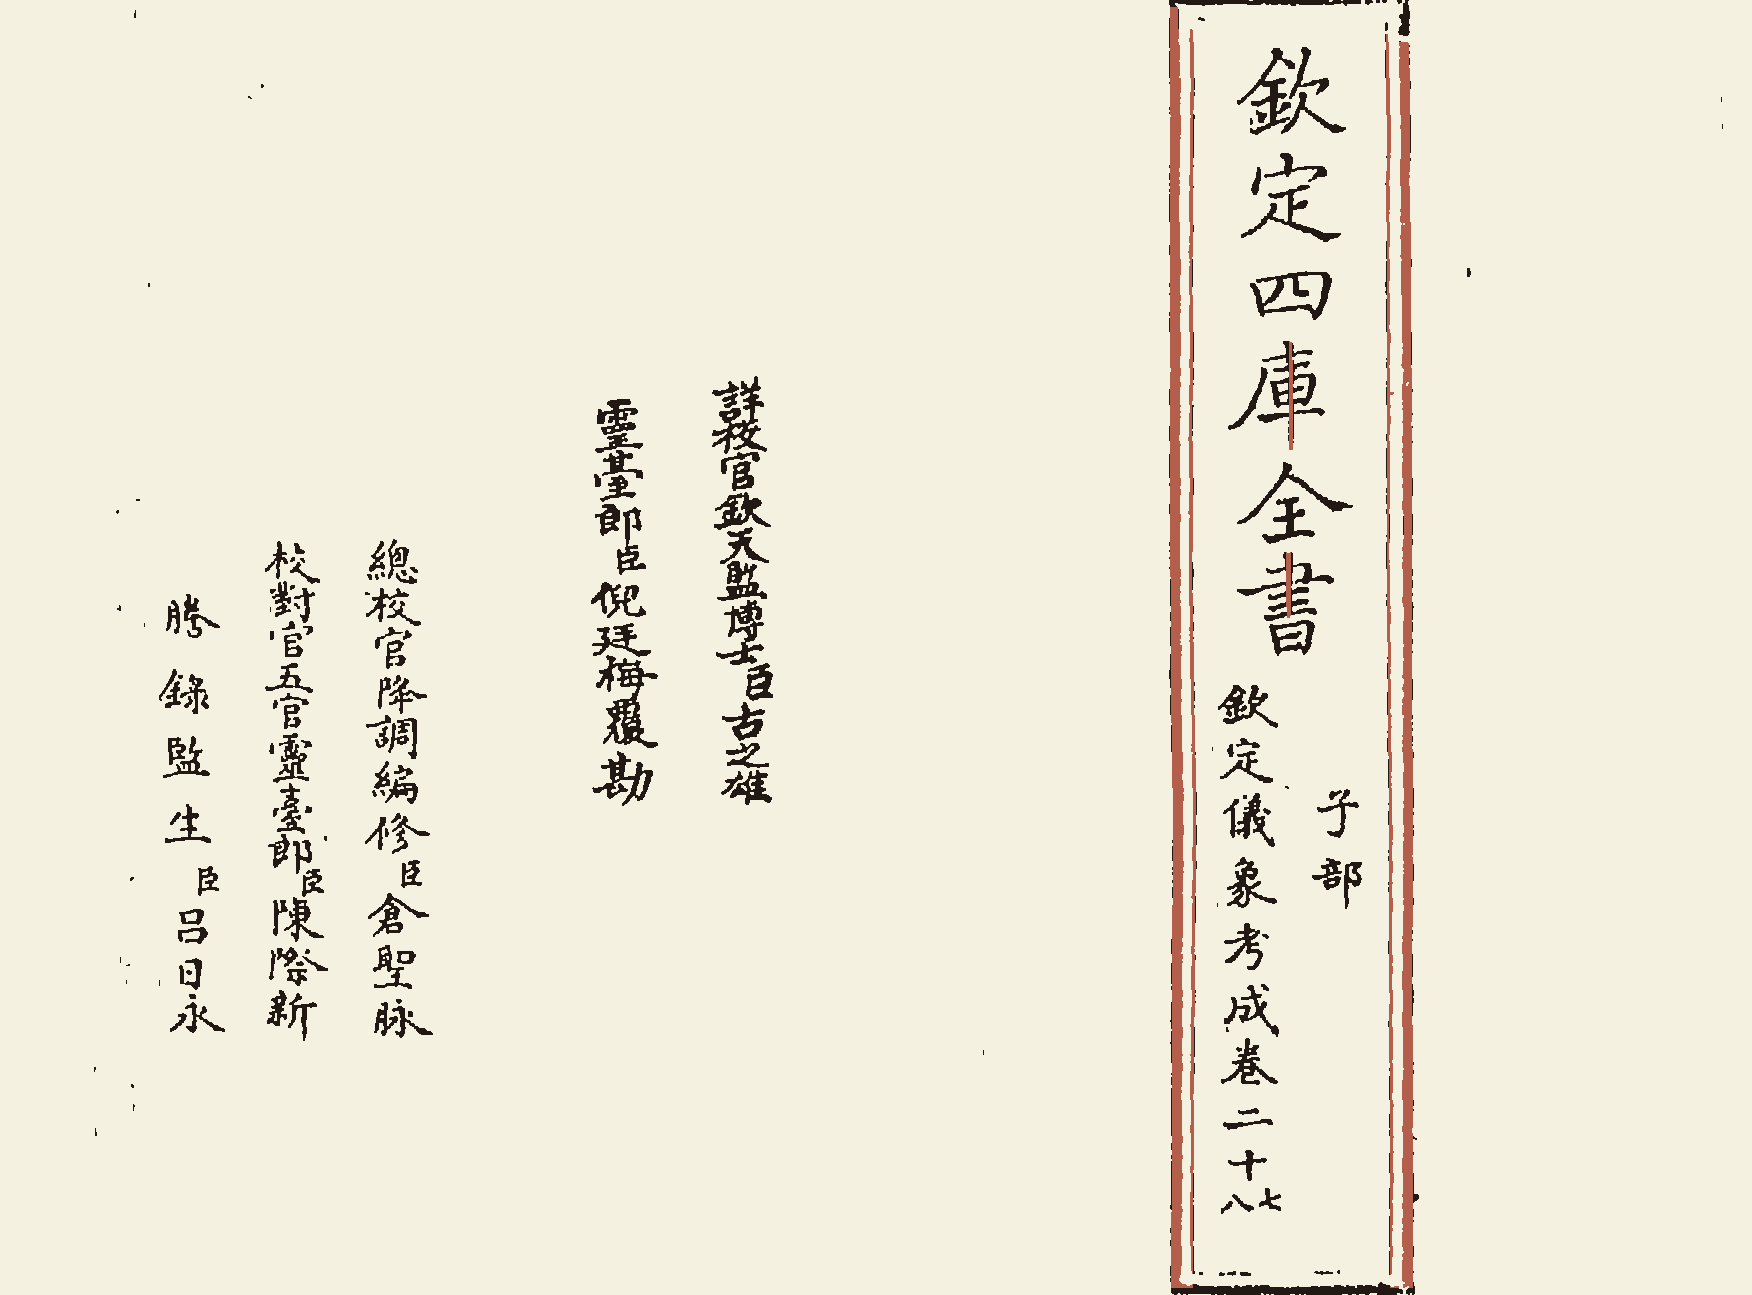
\includegraphics[width=\paperwidth,height=\paperheight,keepaspectratio]{img/1668.png}\clearpage
\begin{正文}
% ---- 册793 葉1669 ----
\SetPageNumber{1}
欽定四庫全書\换行
欽定儀象考成卷二十七\换行
　天漢經緯度表一\换行
　　黄道北天漢度\换行
\char"200B\relax\换行
\char"200B\relax\换行
\char"200B\relax\换行
\char"200B\relax\换行
\char"200B\relax\换行
\char"200B\relax\换行
\char"200B\relax\换行
\char"200B\relax\换行
\char"200B\relax\换行
\char"200B\relax\换行
\char"200B\relax\换行
\char"200B\relax
\par
% ---- 册793 葉1672 ----
　　天漢黄赤經緯度表\换行
晉書天文志云天漢起東方經箕尾之間謂之漢津乃\换行
分為二道其南經傳説魚天籥天弁河鼓其北經龜貫\换行
箕下次絡南斗魁左旗至天津下而合南道乃西南行\换行
又分夾瓠𤓰絡人星杵造父螣蛇王良附路閣道北端\换行
大陵天船卷舌而南行絡五車經北河之南入東井水\换行
位而東南行絡南河闕邱天狗天記天稷至七星南而\换行
没明史天文志云近年浮海之人至赤道以南見雲漢\换行
過天狗之墟抵天社海石之南踰南船帶海山貫十字\换行
\抬头[1]架蜜蜂傍馬腹經南門絡三角龜杵而屬扵尾宿是為帶\换行
\抬头[1]天一周靈䑓儀象志天漢經緯度分列黄道南北赤道南\换行
\抬头[1]北四表與明史合但不按宮次或分二界或分三界或分\换行
\抬头[1]四界逐度列表其分合曲折之處尚有未詳今亦分黄赤\换行
\抬头[1]南北四表而各按宮次分南界北界南之北界北之南界\换行
各列四層其分合既為明晰至其曲折之處經緯或有\换行
不同又扵每度之間細分列表按數圖之庶合懸象云
\par
\end{正文}\clearpage
\嵌图{146.56pt}{202.31pt}{838.64pt}{585.16pt}{img/1673.png}
\begin{正文}
% ---- 册793 葉1673 图版 ----
\SetPageNumber{3}
\插图页
\char"200B\relax\换行
\char"200B\relax\换行
\char"200B\relax\换行
\char"200B\relax\换行
\char"200B\relax\换行
\char"200B\relax\换行
\char"200B\relax\换行
\char"200B\relax\换行
\char"200B\relax\换行
\char"200B\relax\换行
\char"200B\relax\换行
\char"200B\relax\换行
\char"200B\relax\换行
\char"200B\relax\换行
\char"200B\relax\换行
\char"200B\relax
\恢复丝栏\par
\end{正文}\clearpage
\嵌图{144.59pt}{205.10pt}{842.59pt}{579.59pt}{img/1676.png}
\begin{正文}
% ---- 册793 葉1676 图版 ----
\SetPageNumber{4}
\插图页
\char"200B\relax\换行
\char"200B\relax\换行
\char"200B\relax\换行
\char"200B\relax\换行
\char"200B\relax\换行
\char"200B\relax\换行
\char"200B\relax\换行
\char"200B\relax\换行
\char"200B\relax\换行
\char"200B\relax\换行
\char"200B\relax\换行
\char"200B\relax\换行
\char"200B\relax\换行
\char"200B\relax\换行
\char"200B\relax\换行
\char"200B\relax
\恢复丝栏\par
\end{正文}\clearpage
\嵌图{150.52pt}{204.54pt}{830.72pt}{580.72pt}{img/1677.png}
\begin{正文}
% ---- 册793 葉1677 图版 ----
\SetPageNumber{5}
\插图页
\char"200B\relax\换行
\char"200B\relax\换行
\char"200B\relax\换行
\char"200B\relax\换行
\char"200B\relax\换行
\char"200B\relax\换行
\char"200B\relax\换行
\char"200B\relax\换行
\char"200B\relax\换行
\char"200B\relax\换行
\char"200B\relax\换行
\char"200B\relax\换行
\char"200B\relax\换行
\char"200B\relax\换行
\char"200B\relax\换行
\char"200B\relax
\恢复丝栏\par
\end{正文}\clearpage
\嵌图{146.62pt}{204.17pt}{838.53pt}{581.46pt}{img/1680.png}
\begin{正文}
% ---- 册793 葉1680 图版 ----
\SetPageNumber{6}
\插图页
\char"200B\relax\换行
\char"200B\relax\换行
\char"200B\relax\换行
\char"200B\relax\换行
\char"200B\relax\换行
\char"200B\relax\换行
\char"200B\relax\换行
\char"200B\relax\换行
\char"200B\relax\换行
\char"200B\relax\换行
\char"200B\relax\换行
\char"200B\relax\换行
\char"200B\relax\换行
\char"200B\relax\换行
\char"200B\relax\换行
\char"200B\relax
\恢复丝栏\par
\end{正文}\clearpage
\嵌图{144.63pt}{202.37pt}{842.50pt}{585.05pt}{img/1681.png}
\begin{正文}
% ---- 册793 葉1681 图版 ----
\SetPageNumber{7}
\插图页
\char"200B\relax\换行
\char"200B\relax\换行
\char"200B\relax\换行
\char"200B\relax\换行
\char"200B\relax\换行
\char"200B\relax\换行
\char"200B\relax\换行
\char"200B\relax\换行
\char"200B\relax\换行
\char"200B\relax\换行
\char"200B\relax\换行
\char"200B\relax\换行
\char"200B\relax\换行
\char"200B\relax\换行
\char"200B\relax\换行
\char"200B\relax
\恢复丝栏\par
\end{正文}\clearpage
\嵌图{146.56pt}{205.07pt}{838.64pt}{579.65pt}{img/1684.png}
\begin{正文}
% ---- 册793 葉1684 图版 ----
\SetPageNumber{8}
\插图页
\char"200B\relax\换行
\char"200B\relax\换行
\char"200B\relax\换行
\char"200B\relax\换行
\char"200B\relax\换行
\char"200B\relax\换行
\char"200B\relax\换行
\char"200B\relax\换行
\char"200B\relax\换行
\char"200B\relax\换行
\char"200B\relax\换行
\char"200B\relax\换行
\char"200B\relax\换行
\char"200B\relax\换行
\char"200B\relax\换行
\char"200B\relax
\恢复丝栏\par
\end{正文}\clearpage
\嵌图{146.56pt}{203.63pt}{838.64pt}{582.54pt}{img/1685.png}
\begin{正文}
% ---- 册793 葉1685 图版 ----
\SetPageNumber{9}
\插图页
\char"200B\relax\换行
\char"200B\relax\换行
\char"200B\relax\换行
\char"200B\relax\换行
\char"200B\relax\换行
\char"200B\relax\换行
\char"200B\relax\换行
\char"200B\relax\换行
\char"200B\relax\换行
\char"200B\relax\换行
\char"200B\relax\换行
\char"200B\relax\换行
\char"200B\relax\换行
\char"200B\relax\换行
\char"200B\relax\换行
\char"200B\relax
\恢复丝栏\par
\end{正文}\clearpage
\嵌图{146.62pt}{206.54pt}{838.53pt}{576.71pt}{img/1688.png}
\begin{正文}
% ---- 册793 葉1688 图版 ----
\SetPageNumber{10}
\插图页
\char"200B\relax\换行
\char"200B\relax\换行
\char"200B\relax\换行
\char"200B\relax\换行
\char"200B\relax\换行
\char"200B\relax\换行
\char"200B\relax\换行
\char"200B\relax\换行
\char"200B\relax\换行
\char"200B\relax\换行
\char"200B\relax\换行
\char"200B\relax\换行
\char"200B\relax\换行
\char"200B\relax\换行
\char"200B\relax\换行
\char"200B\relax
\恢复丝栏\par
\end{正文}\clearpage
\嵌图{146.62pt}{203.71pt}{838.53pt}{582.37pt}{img/1689.png}
\begin{正文}
% ---- 册793 葉1689 图版 ----
\SetPageNumber{11}
\插图页
\char"200B\relax\换行
\char"200B\relax\换行
\char"200B\relax\换行
\char"200B\relax\换行
\char"200B\relax\换行
\char"200B\relax\换行
\char"200B\relax\换行
\char"200B\relax\换行
\char"200B\relax\换行
\char"200B\relax\换行
\char"200B\relax\换行
\char"200B\relax\换行
\char"200B\relax\换行
\char"200B\relax\换行
\char"200B\relax\换行
\char"200B\relax
\恢复丝栏\par
\end{正文}\clearpage
\嵌图{144.68pt}{200.43pt}{842.41pt}{588.92pt}{img/1692.png}
\begin{正文}
% ---- 册793 葉1692 图版 ----
\SetPageNumber{12}
\插图页
\char"200B\relax\换行
\char"200B\relax\换行
\char"200B\relax\换行
\char"200B\relax\换行
\char"200B\relax\换行
\char"200B\relax\换行
\char"200B\relax\换行
\char"200B\relax\换行
\char"200B\relax\换行
\char"200B\relax\换行
\char"200B\relax\换行
\char"200B\relax\换行
\char"200B\relax\换行
\char"200B\relax\换行
\char"200B\relax\换行
\char"200B\relax
\恢复丝栏\par
\end{正文}\clearpage
\嵌图{146.67pt}{203.58pt}{838.42pt}{582.63pt}{img/1693.png}
\begin{正文}
% ---- 册793 葉1693 图版 ----
\SetPageNumber{13}
\插图页
\char"200B\relax\换行
\char"200B\relax\换行
\char"200B\relax\换行
\char"200B\relax\换行
\char"200B\relax\换行
\char"200B\relax\换行
\char"200B\relax\换行
\char"200B\relax\换行
\char"200B\relax\换行
\char"200B\relax\换行
\char"200B\relax\换行
\char"200B\relax\换行
\char"200B\relax\换行
\char"200B\relax\换行
\char"200B\relax\换行
\char"200B\relax
\恢复丝栏\par
\end{正文}\clearpage
\嵌图{148.48pt}{204.18pt}{834.81pt}{581.44pt}{img/1696.png}
\begin{正文}
% ---- 册793 葉1696 图版 ----
\SetPageNumber{14}
\插图页
\char"200B\relax\换行
\char"200B\relax\换行
\char"200B\relax\换行
\char"200B\relax\换行
\char"200B\relax\换行
\char"200B\relax\换行
\char"200B\relax\换行
\char"200B\relax\换行
\char"200B\relax\换行
\char"200B\relax\换行
\char"200B\relax\换行
\char"200B\relax\换行
\char"200B\relax\换行
\char"200B\relax\换行
\char"200B\relax\换行
\char"200B\relax
\恢复丝栏\par
\end{正文}\clearpage
\嵌图{148.48pt}{203.74pt}{834.81pt}{582.32pt}{img/1697.png}
\begin{正文}
% ---- 册793 葉1697 图版 ----
\SetPageNumber{15}
\插图页
\char"200B\relax\换行
\char"200B\relax\换行
\char"200B\relax\换行
\char"200B\relax\换行
\char"200B\relax\换行
\char"200B\relax\换行
\char"200B\relax\换行
\char"200B\relax\换行
\char"200B\relax\换行
\char"200B\relax\换行
\char"200B\relax\换行
\char"200B\relax\换行
\char"200B\relax\换行
\char"200B\relax\换行
\char"200B\relax\换行
\char"200B\relax
\恢复丝栏\par
\end{正文}\clearpage
\嵌图{145.44pt}{220.43pt}{591.34pt}{572.40pt}{img/1700.png}
\begin{正文}
% ---- 册793 葉1700 ----
\SetPageNumber{16}
\插图页
\char"200B\relax\换行
\char"200B\relax\换行
\char"200B\relax\换行
\char"200B\relax\换行
\char"200B\relax\换行
\char"200B\relax\换行
\char"200B\relax\换行
\char"200B\relax\换行
\恢复丝栏
\char"200B\relax\换行
\char"200B\relax\换行
\char"200B\relax\换行
\char"200B\relax\换行
\char"200B\relax\换行
\char"200B\relax\换行
欽定儀象考成卷二十七\换行
\char"200B\relax
\par

% ======== 卷二十八（8行21字）========
\par\end{正文}\clearpage
\chapter*{欽定儀象考成卷二十八}
\begin{正文}
% ---- 册793 葉1701 ----
\SetPageNumber{1}
欽定四庫全書\换行
欽定儀象考成卷二十八\换行
　天漢經緯度表二\换行
　　黄道南天漢度\换行
\char"200B\relax\换行
\char"200B\relax\换行
\char"200B\relax\换行
\char"200B\relax\换行
\char"200B\relax\换行
\char"200B\relax\换行
\char"200B\relax\换行
\char"200B\relax\换行
\char"200B\relax\换行
\char"200B\relax\换行
\char"200B\relax\换行
\char"200B\relax
\par
\end{正文}\clearpage
\嵌图{146.40pt}{205.08pt}{838.96pt}{579.63pt}{img/1704.png}
\begin{正文}
% ---- 册793 葉1704 图版 ----
\SetPageNumber{2}
\插图页
\char"200B\relax\换行
\char"200B\relax\换行
\char"200B\relax\换行
\char"200B\relax\换行
\char"200B\relax\换行
\char"200B\relax\换行
\char"200B\relax\换行
\char"200B\relax\换行
\char"200B\relax\换行
\char"200B\relax\换行
\char"200B\relax\换行
\char"200B\relax\换行
\char"200B\relax\换行
\char"200B\relax\换行
\char"200B\relax\换行
\char"200B\relax
\恢复丝栏\par
\end{正文}\clearpage
\嵌图{142.61pt}{203.77pt}{846.55pt}{582.24pt}{img/1705.png}
\begin{正文}
% ---- 册793 葉1705 图版 ----
\SetPageNumber{3}
\插图页
\char"200B\relax\换行
\char"200B\relax\换行
\char"200B\relax\换行
\char"200B\relax\换行
\char"200B\relax\换行
\char"200B\relax\换行
\char"200B\relax\换行
\char"200B\relax\换行
\char"200B\relax\换行
\char"200B\relax\换行
\char"200B\relax\换行
\char"200B\relax\换行
\char"200B\relax\换行
\char"200B\relax\换行
\char"200B\relax\换行
\char"200B\relax
\恢复丝栏\par
\end{正文}\clearpage
\嵌图{142.64pt}{202.79pt}{846.47pt}{584.21pt}{img/1708.png}
\begin{正文}
% ---- 册793 葉1708 图版 ----
\SetPageNumber{4}
\插图页
\char"200B\relax\换行
\char"200B\relax\换行
\char"200B\relax\换行
\char"200B\relax\换行
\char"200B\relax\换行
\char"200B\relax\换行
\char"200B\relax\换行
\char"200B\relax\换行
\char"200B\relax\换行
\char"200B\relax\换行
\char"200B\relax\换行
\char"200B\relax\换行
\char"200B\relax\换行
\char"200B\relax\换行
\char"200B\relax\换行
\char"200B\relax
\恢复丝栏\par
\end{正文}\clearpage
\嵌图{144.63pt}{201.77pt}{842.50pt}{586.25pt}{img/1709.png}
\begin{正文}
% ---- 册793 葉1709 图版 ----
\SetPageNumber{5}
\插图页
\char"200B\relax\换行
\char"200B\relax\换行
\char"200B\relax\换行
\char"200B\relax\换行
\char"200B\relax\换行
\char"200B\relax\换行
\char"200B\relax\换行
\char"200B\relax\换行
\char"200B\relax\换行
\char"200B\relax\换行
\char"200B\relax\换行
\char"200B\relax\换行
\char"200B\relax\换行
\char"200B\relax\换行
\char"200B\relax\换行
\char"200B\relax
\恢复丝栏\par
\end{正文}\clearpage
\嵌图{142.64pt}{207.02pt}{846.47pt}{575.75pt}{img/1712.png}
\begin{正文}
% ---- 册793 葉1712 图版 ----
\SetPageNumber{6}
\插图页
\char"200B\relax\换行
\char"200B\relax\换行
\char"200B\relax\换行
\char"200B\relax\换行
\char"200B\relax\换行
\char"200B\relax\换行
\char"200B\relax\换行
\char"200B\relax\换行
\char"200B\relax\换行
\char"200B\relax\换行
\char"200B\relax\换行
\char"200B\relax\换行
\char"200B\relax\换行
\char"200B\relax\换行
\char"200B\relax\换行
\char"200B\relax
\恢复丝栏\par
\end{正文}\clearpage
\嵌图{144.63pt}{205.22pt}{842.50pt}{579.36pt}{img/1713.png}
\begin{正文}
% ---- 册793 葉1713 图版 ----
\SetPageNumber{7}
\插图页
\char"200B\relax\换行
\char"200B\relax\换行
\char"200B\relax\换行
\char"200B\relax\换行
\char"200B\relax\换行
\char"200B\relax\换行
\char"200B\relax\换行
\char"200B\relax\换行
\char"200B\relax\换行
\char"200B\relax\换行
\char"200B\relax\换行
\char"200B\relax\换行
\char"200B\relax\换行
\char"200B\relax\换行
\char"200B\relax\换行
\char"200B\relax
\恢复丝栏\par
\end{正文}\clearpage
\嵌图{142.64pt}{203.74pt}{846.47pt}{582.32pt}{img/1716.png}
\begin{正文}
% ---- 册793 葉1716 图版 ----
\SetPageNumber{8}
\插图页
\char"200B\relax\换行
\char"200B\relax\换行
\char"200B\relax\换行
\char"200B\relax\换行
\char"200B\relax\换行
\char"200B\relax\换行
\char"200B\relax\换行
\char"200B\relax\换行
\char"200B\relax\换行
\char"200B\relax\换行
\char"200B\relax\换行
\char"200B\relax\换行
\char"200B\relax\换行
\char"200B\relax\换行
\char"200B\relax\换行
\char"200B\relax
\恢复丝栏\par
\end{正文}\clearpage
\嵌图{142.64pt}{205.52pt}{846.47pt}{578.76pt}{img/1717.png}
\begin{正文}
% ---- 册793 葉1717 图版 ----
\SetPageNumber{9}
\插图页
\char"200B\relax\换行
\char"200B\relax\换行
\char"200B\relax\换行
\char"200B\relax\换行
\char"200B\relax\换行
\char"200B\relax\换行
\char"200B\relax\换行
\char"200B\relax\换行
\char"200B\relax\换行
\char"200B\relax\换行
\char"200B\relax\换行
\char"200B\relax\换行
\char"200B\relax\换行
\char"200B\relax\换行
\char"200B\relax\换行
\char"200B\relax
\恢复丝栏\par
\end{正文}\clearpage
\嵌图{144.63pt}{200.98pt}{842.50pt}{587.83pt}{img/1720.png}
\begin{正文}
% ---- 册793 葉1720 图版 ----
\SetPageNumber{10}
\插图页
\char"200B\relax\换行
\char"200B\relax\换行
\char"200B\relax\换行
\char"200B\relax\换行
\char"200B\relax\换行
\char"200B\relax\换行
\char"200B\relax\换行
\char"200B\relax\换行
\char"200B\relax\换行
\char"200B\relax\换行
\char"200B\relax\换行
\char"200B\relax\换行
\char"200B\relax\换行
\char"200B\relax\换行
\char"200B\relax\换行
\char"200B\relax
\恢复丝栏\par
\end{正文}\clearpage
\嵌图{146.62pt}{202.38pt}{838.53pt}{585.03pt}{img/1721.png}
\begin{正文}
% ---- 册793 葉1721 图版 ----
\SetPageNumber{11}
\插图页
\char"200B\relax\换行
\char"200B\relax\换行
\char"200B\relax\换行
\char"200B\relax\换行
\char"200B\relax\换行
\char"200B\relax\换行
\char"200B\relax\换行
\char"200B\relax\换行
\char"200B\relax\换行
\char"200B\relax\换行
\char"200B\relax\换行
\char"200B\relax\换行
\char"200B\relax\换行
\char"200B\relax\换行
\char"200B\relax\换行
\char"200B\relax
\恢复丝栏\par
\end{正文}\clearpage
\嵌图{144.59pt}{203.31pt}{842.59pt}{583.17pt}{img/1724.png}
\begin{正文}
% ---- 册793 葉1724 图版 ----
\SetPageNumber{12}
\插图页
\char"200B\relax\换行
\char"200B\relax\换行
\char"200B\relax\换行
\char"200B\relax\换行
\char"200B\relax\换行
\char"200B\relax\换行
\char"200B\relax\换行
\char"200B\relax\换行
\char"200B\relax\换行
\char"200B\relax\换行
\char"200B\relax\换行
\char"200B\relax\换行
\char"200B\relax\换行
\char"200B\relax\换行
\char"200B\relax\换行
\char"200B\relax
\恢复丝栏\par
\end{正文}\clearpage
\嵌图{144.59pt}{202.31pt}{842.59pt}{585.16pt}{img/1725.png}
\begin{正文}
% ---- 册793 葉1725 图版 ----
\SetPageNumber{13}
\插图页
\char"200B\relax\换行
\char"200B\relax\换行
\char"200B\relax\换行
\char"200B\relax\换行
\char"200B\relax\换行
\char"200B\relax\换行
\char"200B\relax\换行
\char"200B\relax\换行
\char"200B\relax\换行
\char"200B\relax\换行
\char"200B\relax\换行
\char"200B\relax\换行
\char"200B\relax\换行
\char"200B\relax\换行
\char"200B\relax\换行
\char"200B\relax
\恢复丝栏\par
% ---- 册793 葉1728 ----
\char"200B\relax\换行
\char"200B\relax\换行
\char"200B\relax\换行
\char"200B\relax\换行
\char"200B\relax\换行
\char"200B\relax\换行
\char"200B\relax\换行
\char"200B\relax\换行
\char"200B\relax\换行
\char"200B\relax\换行
\char"200B\relax\换行
\char"200B\relax\换行
\char"200B\relax\换行
\char"200B\relax\换行
\char"200B\relax\换行
欽定儀象考成卷二十八
\par

\par\end{正文}\clearpage

  \input{parts/part16}
\fi
\end{document}
